\documentclass[12pt, a4paper]{report}
\usepackage{Custom}

\makenomenclature
\makeindex[intoc=true,options=-s index]

\begin{document}

\hypersetup{allcolors = black}

\title{Compendium of Mathematics \& Physics}
\author{Nicolas Dewolf}
\maketitle

\dominitoc
\doparttoc
\tableofcontents

\hypersetup{allcolors = UGent}

\chapter*{Introduction}
\markboth{Introduction}
\mtcaddchapter
\section*{Goals}

   This compendium originated out of the necessity for a compact summary of important theorems and formulas during physics and mathematics classes at university. When the interest in more (and more exotic) subjects grew, this collection lost its compactness and became the chaos it now is. Although there should exist some kind of overall structure, it was not always possible to keep every section self-contained or respect the order of the chapters.

   It should definitely not be used as a formal introduction to any subject. It is neither a complete work nor a fact-checked one, so the usefulness and correctness is not guaranteed. However, it can be used as a look-up table for theorems and formulas, and as a guide to the literature. To this end, each chapter begins with a list of useful references. At the same time, only a small number of statements are proven in the text (or appendices). This was done to keep the text as concise as possible (a failed endeavour). However, in some cases the major ideas underlying the proofs are provided.

\section*{Structure and conventions}

   Sections and statements that require more advanced concepts, in particular concepts from later chapters or (higher) category theory, will be labelled by the \textit{clubs} symbol~$\clubsuit$. Some definitions, properties or formulas are given with a proof or an extended explanation whenever I felt like it. These are always contained in a blue frame to make it clear that they are not part of the general compendium. When a section uses notions or results from a different chapter at its core, this will be recalled in a green box at the beginning of the section.

   Definitions in the body of the text will be indicated by the use of \textbf{bold font}. Notions that have not been defined in this summary but that are relevant or that will be defined further on in the compendium (in which case a reference will be provided) are indicated by \textit{italic text}. Names of authors are also written in \textit{italic}.

   Objects from a general category will be denoted by a lower-case letter (depending on the context, upper-case might be used for clarity), functors will be denoted by upper-case letters and the categories themselves will be denoted by symbols in \textbf{bold font}. In the later chapters on physics, specific conventions for the different types of vectors will often be adopted. Vectors in Euclidean space will be denoted by a bold font letter with an arrow above, e.g.~$\vector{a}$, whereas vectors in Minkowski space (4-vectors) and differential forms will be written without the arrow, e.g.~$\symbf{a}$. Matrices and tensors will always be represented by capital letters and, dependent on the context, a specific font will be adopted.

% \part{Set Theory, Algebra \& Category Theory}
% \insertparttoc

% \chapter{Set Theory}

    \minitoc

\section{Axiomatization}\label{section:axiomatization}
\subsection{ZFC}

    The following set of axioms and axiom schemata gives a foundation for axiomatic set theory whilst fixing a number of issues in naive set theory, where the notion of a set is taken for granted. This theory is called \textbf{Zermelo--Frenkel} set theory (ZF). When extended with the axiom of choice (see further on), it is called ZFC, where the C stand for `choice'.

    \begin{axiom}[Power set]\index{power!set}\label{set:power_set_axiom}
        \begin{gather}
            \forall x:\exists y:\forall z\bigl(z\in y\iff\forall w(w\in z\implies w\in x)\bigr)
        \end{gather}
        The set $y$ is called the power set $P(x)$ or $2^x$ of $x$.
    \end{axiom}

    \begin{axiom}[Extensionality]\index{extensionality}
        \begin{gather}
            \forall x,y:\forall z\bigl(z\in x\iff z\in y\bigr)\implies x=y
        \end{gather}
        This axiom allows to compare two sets based on their elements, i.e.~two sets are (strictly) equal if and only if they have the same elements.
    \end{axiom}
    \begin{remark}
        As will be made clear throughout this document, strict equality as in the extensionality axiom is often not what one cares about in practice. \textit{Equivalence} and \textit{isomorphism} will be the practically relevant notions.
    \end{remark}

    \begin{axiom}[Regularity\footnotemark]\index{regularity}
        \footnotetext{Also called the \textbf{axiom of foundation}.}
        \begin{gather}
            \forall x:(\exists z\in x)\implies(\exists a\in x)\land\neg(\exists b\in a:b\in x)
        \end{gather}
        This axiom says that for every nonempty set $x$, one can find an element $a\in x$ such that $x$ and $a$ are disjoint. Among other things, this axiom implies that no set can contain itself.
    \end{axiom}

    The following axiom is technically not an axiom but an axiom schema, i.e.~for every predicate $\varphi$, one obtains an axiom.
    \begin{axiom}[Specification]\index{specification}
        \begin{gather}
            \forall w_1,\ldots,w_n,A:\exists B:\forall x\bigl[x\in B\iff\bigl(x\in A\land\varphi(x,w_1,\ldots,w_n,A)\bigr)\bigr]
        \end{gather}
        This axiom (schema) says that, for every set $x$, one can build another set of elements in $x$ that satisfy a given predicate. By the axiom of extensionality, this subset $B\subseteq A$ is unique.
    \end{axiom}
    \begin{notation}[Set builder notation]\index{set!builder notation}
        The sets constructed through the axiom of specification are often denoted as follows:
        \begin{gather}
            B=\{x\in A\mid\phi(x)\}\,,
        \end{gather}
        where the parameters $w_1,\ldots,w_n$ were suppressed for conciseness.
    \end{notation}

\subsection{Material set theory}\index{set theory!material}

    ZF(C) is an instance of \textit{material set theory}. Every element of a set is itself a set and, hence, possesses some kind of internal structure.

    \newdef{Pure set}{\index{pure!set}
        A set $U$ such that, for every sequence
        \begin{gather}
            x_n\in x_{n-1}\in\cdots\in x_1\in U\,,
        \end{gather}
        all elements $x_i$ are also sets.
    }
    \newdef{Urelement\footnotemark}{\index{urelement}\index{atom}
        \footnotetext{Sometimes called an \textbf{atom}.}
        An object that is not a set.
    }

    \todo{COMPLETE}

\subsection{Structural set theory}\index{set theory!structural}

    In contrast to material set theory, the fundamental notions in this theory are the relations between sets. An element of a set does not have any internal structure and only becomes relevant if one specifies extra structure (given by relations) on the sets. This implies that elements of sets are not sets themselves. In fact, this would be a meaningless statement since, by default, they lack any internal structure. Even stronger, it is meaningless to compare two elements if one does not provide relations or extra structure on the sets.

    \todo{COMPLETE}

\subsection{\texorpdfstring{ETCS $\clubsuit$}{ETCS}}

    \sremark{ETCS is the abbreviation of `Elementary Theory of the Category of Sets'.}

    \begin{axiom}
        The category of sets is a \textit{well-pointed (elementary) topos} (see \cref{chapter:topos}).
    \end{axiom}

    \todo{COMPLETE}

\subsection{Universes}\label{section:universes}

    To be able to talk about sets without running into problems such as \textit{Russel's paradox}, where one needs (or wants) to talk about the collection of all things satisfying a certain condition, one can introduce the concept of a `universal set' or `universe (of discourse)'. This set takes the place of the `collection of things' and all operations act within this universe.

    \newdef{Grothendieck universe}{\index{Grothendieck!universe}
        A pure set $U$ satisfying the following conditions:
        \begin{enumerate}
            \item\textbf{Transitivity}: If $x\in U$ and $y\in x$, then $y\in U$.
            \item\textbf{Power set}: If $x\in U$, then $P(x)\in U$.
            \item\textbf{Pairing}: If $x,y\in U$, then $\{x,y\}\in U$.
            \item\textbf{Unions}: If $I\in U$ and $\{x_i\}_{i\in I}\subset U$, then $\bigcup_{i\in I}x_i\in U$.
        \end{enumerate}
    }

\section{Finite sets}

    \newdef{Bishop finiteness}{\index{finite!set}\index{Bishop|see{finite set}}
        A set $S$ is said to be (Bishop) finite if there exists a bijection $S\cong[n]$ for some $n\in\mathbb{N}$.
    }

    In ZFC, any other reasonable definition of finite sets will be equivalent to the one above. However, in constructive mathematics, this is not true anymore. Because the \textit{internal logic} of \textit{elementary topoi} (see \cref{chapter:topos}) is constructive, some more information is given here.

    \newdef{Kuratowski finiteness}{\index{Kuratowski|see{finite set}}
        A set $S$ is said to be Kuratowski finite or \textbf{finitely indexed set} if there exists a surjection $[n]\twoheadrightarrow S$ for some $n\in\mathbb{N}$.
    }

    \newdef{Dedekind finiteness}{\index{Dedekind|see{finite set}}
        A set $S$ is said to be Dedekind finite if any injection $S\hookrightarrow S$ is a bijection.
    }

    \todo{COMPLETE}

\section{Real numbers}\index{real numbers}

    \begin{axiom}[Ordering]
        The set of real numbers is an \textit{ordered field} (see \cref{algebra:field}).
    \end{axiom}
    \begin{axiom}[Dedekind completeness]\index{Dedekind!completeness}\label{set:dedekind_completeness}
        Every nonempty subset of $\mathbb{R}$ that is bounded from above has a \textit{supremum} (see \cref{set:supremum} and \cref{set:complete_lattice}).
    \end{axiom}

    \begin{axiom}
        The rational numbers form a subset of the real numbers: $\mathbb{Q}\subset\mathbb{R}$.
    \end{axiom}

    \begin{remark}
        There is only one way (up to isomorphisms) to extend the field of rational numbers to the field of reals such that it satisfies the previous axioms.
    \end{remark}

    \newdef{Extended real line}{\label{calculus:extended_real_line}
        \begin{gather}
            \overline{\mathbb{R}} := \mathbb{R}\cup\{-\infty,\infty\} \equiv [-\infty,\infty]
        \end{gather}
    }

\section{Set operations}

    \newdef{Cartesian product}{\index{product}
        Let $X,Y$ be two sets. Their (Cartesian) product is defined as follows:
        \begin{gather}
            X\times Y := \{(x,y)\mid x\in X\land y\in Y\}\,.
        \end{gather}
    }

    \newdef{Symmetric difference}{\index{symmetric!difference}\label{set:symmetric_difference}
        \begin{gather}
            A\Delta B := (A\backslash B)\cup(B\backslash A)
        \end{gather}
    }

    \newdef{Diagonal}{\index{diagonal}
        The diagonal of a set $X$ is defined as follows:
        \begin{gather}
            \Delta_X := \bigl\{(x,x)\in X\times X\bigm\vert x\in X\bigr\}\,.
        \end{gather}
    }

    \newdef{Complement}{\index{complement}\label{set:complement}
        Let $\Omega$ be the universe of discours (\cref{section:universes}) and consider $X\subseteq\Omega$. The complement of $X$ is defined as follows:
        \begin{gather}
            X^c := \Omega\backslash X\,.
        \end{gather}
    }

    \newformula{de Morgan's laws}{\index{de Morgan!law}
        \begin{gather}
            \label{set:de_morgan_union}
            \left(\bigcup_iX_i\right)^c = \bigcap_iX_i^c
        \end{gather}
        \begin{gather}
            \label{set:de_morgan_intersection}
            \left(\bigcap_iX_i\right)^c = \bigcup_iX_i^c
        \end{gather}
    }

    \newdef{Relation}{\index{relation}\label{set:relation}
        A relation between two sets $X$ and $Y$ is a subset of the Cartesian product $X\times Y$. A relation on $X$ is then simply a subset of $X\times X$. This definition can easily be extended to $n$-ary relations by working with subsets of $n$-fold products.
    }

    \newdef{Converse relation}{\index{converse}\label{set:converse}
        Consider a relation $R\subseteq X\times Y$. The converse relation $R^t$ is defined as follows:
        \begin{gather}
            R^t := \bigl\{(y,x)\in Y\times X\bigm\vert(x,y)\in R\bigr\}\,.
        \end{gather}
    }
    \newdef{Composition of relations}{\index{composition!of relations}\label{set:relational_composition}
        Consider two relations $R\subseteq X\times Y$ and $S\subseteq Y\times Z$ between three sets $X,Y$ and $Z$. The composition $S\circ R$ is defined as follows:
        \begin{gather}
            S\circ R := \bigl\{(x,z)\in X\times Z\bigm\vert\exists y\in Y:(x,y)\in R\land(y,z)\in S\bigr\}.
        \end{gather}
    }

\section{Functions}
\subsection{(Co)domain}

    \newdef{Domain}{\index{domain}\label{set:domain}
        Let $f:X\rightarrow Y$ be a function. The set $X$ is called the domain of $f$.
    }
    \begin{notation}
        The domain of $f$ is denoted by $\mathrm{dom}(f)$.
    \end{notation}

    \newdef{Support}{\index{support}
        Let $f:X\rightarrow\mathbb{R}$ be a function. The support of $f$ is defined as the set of points where $f$ is nonzero.
    }
    \begin{notation}
        The support of $f$ is denoted by $\supp(f)$.
    \end{notation}

    \begin{notation}\label{set:function_set}
        Let $X,Y$ be two sets. The set of functions $f:X\rightarrow Y$ is denoted by $Y^X$ or $\mathrm{Map}(X,Y)$. (See also \cref{cat:exponential_object} for a generalization.)
    \end{notation}

    \newdef{Codomain}{\index{co-!domain}
        Let $f:X\rightarrow Y$ be a function. The set $Y$ is called the codomain of $f$.
    }
    \newdef{Image}{\index{image}
        Let $f:X\rightarrow Y$ be a function. The following subset of $Y$ is called the image of $f$:
        \begin{gather}
            \im(f):=\{y\in Y\mid\exists x\in X:f(x) = y\}\,.
        \end{gather}
    }
    \sremark{Some authors use the notions of codomain and image interchangeably.}

    \newdef{Level set}{\index{level!set}\index{fibre}\index{pre-!image}\label{set:level_set}
        Consider a function $f:X\rightarrow\mathbb{R}$. The following set is called the level set of $f$ at $c\in\mathbb{R}$:
        \begin{gather}
            f^{-1}(c) := \{x\in X\mid f(x) = c\}\,.
        \end{gather}
        For $X=\mathbb{R}^2$ the level sets are called \textbf{level curves} and for $X=\mathbb{R}^3$ they are called \textbf{level surfaces}. More generally, for functions $f:X\rightarrow Y$, one calls $f^{-1}(y)$ the \textbf{preimage} or \textbf{fibre} of $f$ over $y$.
    }

\subsection{Functions}

    \newdef{Injective}{\index{injective}\index{one-to-one|see{injective}}\label{set:injective}
        A function $f:A\rightarrow B$ is said to be injective or \textbf{one-to-one} if the following condition is satisfied:
        \begin{gather}
            \forall a,a'\in A:f(a)=f(a')\implies a=a'\,.
        \end{gather}
    }
    \newnot{Injective function}{\[f:A\hookrightarrow B\]}

    \newdef{Surjective}{\index{surjective}\index{onto|see{surjective}}\label{set:surjective}
        A function $f:A\rightarrow B$ is said to be surjective or \textbf{onto} if the following condition is satisfied:
        \begin{gather}
            \forall b\in B:\exists a\in A:f(a) = b\,.
        \end{gather}
    }
    \newnot{Surjective function}{\[f:A\twoheadrightarrow B\]}

    \newdef{Bijection}{\index{bijection}
        A function that has an inverse. Equivalently, a function that gives a one-to-one correspondence between the elements of the domain and those of the codomain.
    }
    \newnot{Isomorphic sets}{
        \[X\cong Y\]
    }

    \begin{theorem}[Cantor--Bernstein--Schr\"oder]\index{Cantor--Bernstein--Schr\"oder}\label{set:CBS_theorem}
        Consider two sets $A,B$. If there exist injections $A\hookrightarrow B$ and $B\hookrightarrow A$, there exists a bijection $A\cong B$.
    \end{theorem}

    \newdef{Involution}{\index{involution}\label{set:involution}
        A function $f:A\rightarrow A$ such that $f^2=\mathbbm{1}_A$, i.e.~$f$ is its own inverse. Every involution is, in particular, a bijection.
    }

\section{Collections}
\subsection{Families and filters}\label{section:collections}

    \newdef{Power set}{\index{power!set}\label{set:power_set}
        Let $X$ be a set. The power set is defined as the set of all subsets of $X$ and is (often) denoted by $P(X)$ or $2^X$. The existence of this set is enforced by the power set axiom (\cref{set:power_set_axiom}).
    }
    \result{All sets are elements of their power set: $X\in P(X)$.}

    \newdef{Collection}{\index{collection}\index{index!set}
        A collection of elements of a set $X$ is a subset of $X$. Often, this collection is indexed by some \textbf{index set} $I$, in which case it is often denoted as $\{x_i\}_{i\in I}\subseteq X$.
    }
    \newdef{Family}{\index{family}\index{index!set}
        Let $X,I$ be two sets. A family of elements of $X$ with \textbf{index set} $I$ is a function $f:I\rightarrow X$. A family with index set $I$ is often denoted by $(x_i)_{i\in I}$. In contrast to collections, a family can contain multiple copies of the same element.
    }

    \todo{CHECK COMPENDIUM TO GET NOTATIONS STRAIGHT}

    \newdef{Helly family}{\index{Helly!family}\label{set:helly_family}
        A Helly family of order $k\in\mathbb{N}$ is a pair $(X,F)$ with $F\subset P(X)$ such that for every finite $G\subset F$:
        \begin{gather}
            \bigcap_{V\in G}V = \emptyset\implies\exists H\subseteq G: \left(\bigcap_{V\in H}V = \emptyset\right)\land\Bigl(|H|\leq k\Bigr)\,.
        \end{gather}
        A Helly family of order 2 is sometimes said to have the \textbf{Helly property}.

        \todo{WHERE IS THIS NEEDED?}
    }

    \newdef{Cover}{\index{cover}\label{set:cover}
        A cover of a set $X$ is a collection of sets $\{V_i\}_{i\in I}\subseteq P(X)$ such that:
        \begin{gather}
            \bigcup_{i\in I}V_i=X\,.
        \end{gather}
    }

    \newdef{Partition}{\index{partition}
        A  partition of $X$ is a collection of disjoint subsets $\{A_i\}_{i\in I}\subset P(X)$ such that $\bigcup_{i\in I}A_i=X$, i.e.~it is a disjoint cover.
    }
    \newdef{Refinement}{\index{refinement}
        Let $P$ be a partition of $X$. A refinement $P'$ of $P$ is a collection of subsets such that every $A\in P$ can be written as a disjoint union of elements in $P'$. It follows that every refinement is also a partition.
    }

    \newdef{Filter}{\index{filter}\label{set:filter}
        Let $X$ be a set. A family $\mathcal{F}\subseteq P(X)$ is a filter on $X$ if it satisfies the following conditions:
        \begin{enumerate}
            \item\textbf{Nonemptiness}: $\emptyset\not\in\mathcal{F}$.
            \item\textbf{Downward closure}: $\forall A,B \in\mathcal{F}:A\cap B\in\mathcal{F}$.
            \item\textbf{Isotony}: if $A\in\mathcal{F}$ and $A\subseteq B$, then $B\in\mathcal{F}$.
        \end{enumerate}
    }

    \newdef{Filtration}{\index{filtration}\label{set:filtration}
        Consider a set $X$ together with a collection of subsets $\{F_i\}_{i\in I}$ indexed by a \textit{totally ordered set} $I$ (see \cref{set:total_order}). The collection is said to be a filtration of $X$ if
        \begin{gather}
            i\leq j\implies F_i\subseteq F_j\,.
        \end{gather}
        A filtration is said to be \textbf{exhaustive} if $\bigcup_{i\in I}F_i=X$ and \textbf{separated} if $\bigcap_{i\in I}F_i=\emptyset$.
    }
    \newdef{Associated grading}{\index{graded!object}
        When one can define \textit{quotient objects}, every filtration $\{F_i\}_{i\in I}$ of $X$ defines an associated graded object $\{G_i := F_i/F_{i-1}\}_{i\in I}$.
    }

\subsection{Algebra of sets}

    \newdef{Algebra of sets}{\index{algebra!of sets}\index{field!of sets|see{algebra}}\index{Boolean!algebra}\label{set:algebra_of_sets}
        A collection $\mathcal{F}\subset P(X)$ is a called an algebra over $X$ if it satisfies the following conditions:
        \begin{enumerate}
            \item\textbf{Totality}: $X\in\mathcal{F}$,
            \item\textbf{Closed under complements}: $\forall E\in\mathcal{F}:E^c\in\mathcal{F}$, and
            \item\textbf{Closed under finite unions}: $\forall E,E'\in\mathcal{F}:E\cup E'\in\mathcal{F}$.
        \end{enumerate}
        The pair $(X,\mathcal{F})$ is also called a \textbf{field of sets} or \textbf{concrete Boolean algebra}.
    }

    Extending this definition to closure under countable unions gives another common notion.
    \newdef{$\sigma$-algebra}{\index{$\sigma$!algebra}\index{measurable}\label{set:sigma_algebra}
        A collection $\Sigma\subset P(X)$ is called a $\sigma$-algebra over a set $X$ if it satisfies the following conditions:
        \begin{enumerate}
            \item\textbf{Totality}: $X\in\Sigma$,
            \item\textbf{Closed under complements}: $\forall E\in\Sigma: E^c\in\Sigma$, and
            \item\textbf{Closed under countable unions}: $\forall\{E_n\}_{n\in\mathbb{N}}\subset\Sigma:\bigcup_{n=1}^{+\infty}E_n\in\Sigma$.
        \end{enumerate}
        The pair $(X,\Sigma)$ is called a \textbf{measurable space}. The elements $E\in\Sigma$ are called \textbf{measurable sets}.
    }
    \begin{remark}
        Conditions 1 and 2 imply that both $\sigma$-algebra and fields of sets always contain the empty set. Conditions 2 and 3, together with de Morgan's laws~\eqref{set:de_morgan_union} and~\eqref{set:de_morgan_intersection}, imply that a $\sigma$-algebra is also closed under countable intersections and, analogously, that a field of sets is closed under finite intersections.
    \end{remark}

    \begin{property}[Intersections]
        The intersection of a collection of $\sigma$-algebras is again a $\sigma$-algebra.
    \end{property}

    \newdef{Generated $\sigma$-algebras}{\label{set:generated_sigma_algebra}
        A $\sigma$-algebra $\mathcal{G}$ is said to be generated by a collection of sets $\mathcal{A}$ if
        \begin{gather}
            \mathcal{G} = \bigcap\{\mathcal{F}\mid\mathcal{F}\text{ is a } \sigma\text{-algebra that contains }\mathcal{A}\}\,.
        \end{gather}
        Equivalently, it is the smallest $\sigma$-algebra containing $\mathcal{A}$.
    }
    \begin{notation}\label{set:notation:generated_sigma_algebra}
        The $\sigma$-algebra generated by a collection of sets $\mathcal{A}$ is often denoted by $\sigma(\mathcal{A})$.
    \end{notation}

    \newdef{Product $\sigma$-algebras}{\label{set:product_of_sigma_algebras}
        The product $\sigma$-algebra $\mathcal{F}_1\otimes\mathcal{F}_2$ on $X_1\times X_2$ can be defined in the following equivalent ways:
        \begin{itemize}
            \item $\mathcal{F}$ is generated by $\{A_1\times\Omega_2\mid A_1\in\mathcal{F}_1\}\cup\{\Omega_1\times A_2\mid A_2\in\mathcal{F}_2\}$.
            \item $\mathcal{F}$ is generated by $\{A_1\times A_2\mid A_1\in\mathcal{F}_1\land A_2\in\mathcal{F}_2\}$.
        \end{itemize}
    }

    \newdef{Monotone class}{\index{monotone!class}
        A collection of sets $\mathcal{A}$ that has the following two properties:
        \begin{enumerate}
            \item For every increasing sequence $A_1\subset A_2\subset\cdots$ : $\bigcup_{n=1}^{+\infty}A_n\in\mathcal{A}$.
            \item For every decreasing sequence $A_1\supset A_2\supset\cdots$ : $\bigcap_{n=1}^{+\infty}A_n\in\mathcal{A}$.
        \end{enumerate}
    }

    \begin{theorem}[Monotone class theorem]\label{set:monotone_class}
        Let $\mathcal{A}$ be an algebra of sets. If $\mathcal{G}_{\mathcal{A}}$ is the smallest monotone class containing $\mathcal{A}$, it coincides with the $\sigma$-algebra generated by $\mathcal{A}$.
    \end{theorem}

\section{Ordered sets}\index{order}\label{section:ordered_sets}
\subsection{Posets}

    \newdef{Partially ordered set}{\index{poset}\index{pre-!order|see{order}}\label{set:poset}
        A set $P$ equipped with a binary relation $\leq$ is called a partially ordered set (or \textbf{poset}) if the following 3 conditions are satisfied for all elements $x,y,z\in P$:
        \begin{enumerate}
            \item\textbf{Reflexivity}: $x\leq x$,
            \item\textbf{Antisymmetry}: $x\leq y\land y\leq x\implies x=y$, and
            \item\textbf{Transitivity}: $x\leq y\land y\leq z\implies x\leq z$.
        \end{enumerate}
        If the antisymmetry condition is dropped, a \textbf{preorder} is obtained.
    }

    \newdef{Order-preserving map}{\index{monotone!function}\index{order!-preserving}
        A function $f:(P,\leq)\rightarrow(P',\preceq)$ of posets such that $x\leq y\implies f(x)\preceq f(y)$ for all $x,y\in P$. These functions are also said to be \textbf{monotone}.
    }

    \newdef{Hasse diagram}{\index{Hasse diagram}
        Consider a finite poset $(P,\leq)$. A Hasse diagram for $P$ is a \textit{graph} where the vertices are given by the elements of $P$ and two vertices $x,y$ are connected upwardly if and only if $x\leq y$ in $P$.
    }
    \begin{example}
        Consider the power set of $\{0,1\}$ with its canonical poset structure. A Hasse diagram of this poset is
        \begin{gather*}
            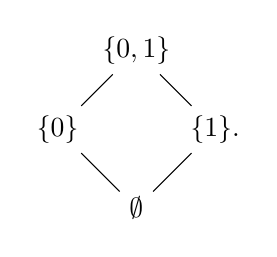
\begin{tikzpicture}
                \node (01) at (0, 0) {$\{0,1\}$};
                \node (0) at (-1, -1) {$\{0\}$};
                \node (1) at (1, -1) {$\{1\}.$};
                \node (empty) at (0, -2) {$\emptyset$};
                \draw (empty) -- (0) -- (01);
                \draw (empty) -- (1) -- (01);
            \end{tikzpicture}
        \end{gather*}
    \end{example}

    \newdef{Totally ordered set}{\index{totality}\label{set:total_order}
        A poset $P$ with the property that for all $x,y\in P$, either $x\leq y$ or $y\leq x$. This property is called \textbf{totality}.
    }
    \newdef{Strict total order}{
        A nonstrict order $\leq$ has an associated strict order $<$ that satisfies $x<y\iff x\leq y\land x\neq y$.
    }

    \newdef{Linear order}{
        A binary relation $<$ on a set $P$ satisfying the following conditions for all $x,y,z\in P$:
        \begin{enumerate}
            \item\textbf{Irreflexivity}: $x\not<x$,
            \item\textbf{Asymmetry}: $x<y\implies y\not<x$,
            \item\textbf{Transitivity}: $x<y\land y<z\implies x<z$,
            \item\textbf{Comparison}: $x<z\implies x<y\lor y<z$, and
            \item\textbf{Connectedness}: $x\not<y\land y\not<x\implies x=y$.
        \end{enumerate}
    }
    \remark{By negation, one can freely pass between linear orders and total orders. However, without the law of the excluded middle, there exists no bijection between them.}

    \newdef{Supremum}{\index{supremum}\label{set:supremum}
        The supremum $\sup(P)$ of a poset $P$ is the least upper bound of $P$.
    }
    \newdef{Infimum}{\index{infimum}\label{set:infimum}
        The infimum $\inf(P)$ of a poset $P$ is the greatest lower bound of $P$.
    }

    \newdef{Maximum}{\index{maximum}\label{set:maximum}
        If $\sup(P)\in P$, the supremum is called the maximum of $P$. This is denoted by $\max(P)$.
    }
    \newdef{Minimum}{\index{minimum}\label{set:minimum}
        If $\inf(P)\in P$, the supremum is called the minimum of $P$. This is denoted by $\min(P)$.
    }

    \newdef{Chain}{\index{chain}\label{set:chain}
        A totally ordered subset of a poset.
    }
    \begin{theorem}[Zorn's lemma\footnotemark]\index{Zorn's lemma}\label{set:zorns_lemma}
        \footnotetext{This theorem is equivalent to the \textit{axiom of choice}.}
        Let $(P,\leq)$ be a poset. If every chain in $P$ has an upper bound in $P$, then $P$ has a maximal element.
    \end{theorem}

    \newdef{Directed\footnotemark\ set}{\index{directed set}\index{filtered set|see{directed set}}\label{set:directed_set}
        \footnotetext{Sometimes called a \textbf{filtered} set or \textbf{upward} directed set. \textbf{Downward} directed sets are analogously defined with a lower bound for every two elements.}
        A set $P$ equipped with a preorder $\leq$ with the additional property that every 2-element subset has an upper bound, i.e.~for every two elements $x,y\in P$, there exists an element $z\in P$ such that $x\leq z\land y\leq z$.
    }
    \newdef{Net}{\index{net}\label{set:net}
        A net on a set $X$ is a subset of $X$ indexed by a directed set $I$.
    }

    \newdef{Cut}{\index{cut}\index{Dedekind!cut}\index{union!ordered}
        Let $(P,\leq)$ be a totally ordered set. A cut or \textbf{decomposition} of $P$ is a pair $(A,B)$ of disjoint subsets such that $P=A\cup B$ in the ordered sense, i.e.~every element of $A$ is smaller than every element of $B$. Cuts can be classified as follows:
        \begin{itemize}
            \item\textbf{Jumps}: $A$ has a greatest element and $B$ has a least element.
            \item\textbf{Dedekind cut}: Either $A$ has a greatest element and $B$ has no least element or $A$ has no greatest element, but $B$ has a least element.
            \item\textbf{Gap}: $A$ has no greatest element and $B$ has no least element.
        \end{itemize}
    }

    The notion of a filter on a set $X$ (\cref{set:filter}) is a specific example of a more general notion, where the underlying poset is the power set of $X$.
    \newdef{Filter}{\index{filter}\index{ultrafilter}\label{set:ultrafilter}
        Let $X$ be a poset. A filter on $X$ is a subset $\mathcal{F}\subseteq X$ such that:
        \begin{enumerate}
            \item\textbf{Nonemptiness}: $\mathcal{F}\neq\emptyset$,
            \item\textbf{Downward closure}: $\forall x,y\in\mathcal{F}:\exists z\in\mathcal{F}:z\leq x\land z\leq y$, and
            \item\textbf{Isotony}: If $x\in\mathcal{F}$ and $x\leq y$, then $y\in\mathcal{F}$.
        \end{enumerate}
        If there exists no strictly greater filter $\mathcal{F}\subset\mathcal{F}'$, then $\mathcal{F}$ is called an \textbf{ultrafilter}.
    }

    The following theorem is independent of the ZF axioms, but strictly weaker than the \textit{axiom of choice}.
    \begin{theorem}[Ultrafilter lemma]
        Every proper filter on a set is contained in an ultrafilter.
    \end{theorem}

\subsection{\difficult{Ordinals}}

    \newdef{Well-ordering}{\index{well-!order}\index{well-!founded}
        A \textbf{well-founded} linear order, i.e.~a linear order such that every nonempty subset has a minimal element.
    }

    \newdef{Ordinal number}{\index{number!ordinal}\label{set:ordinal}
        Consider the class of all well-ordered sets. An ordinal (type or rank) is an isomorphism class of well-ordered sets. The class of ordinals is itself well ordered by inclusion of `initial segments'.

        However, this definition gives problems within the ZF(C) framework of set theory, since these equivalence classes are proper classes and not sets. To overcome this problem, one can use a different approach. By using a well-defined construction, one can, for every class, select a particular representative and call this representative the \textbf{ordinal number} of all well-ordered sets isomorphic to it.
    }

    The most common construction is the one by \indexauthor{von Neumann}. For every well-ordered set $W$, there exists a function
    \begin{gather}
        W\rightarrow P(W):w\mapsto W_{\leq w}:=\{w'\in W\mid w'\leq w\}
    \end{gather}
    that restricts to an order isomorphism on its image. This leads to the following definition.
    \newdef{von Neumann ordinal}{\index{von Neumann!ordinal}
        A set that is strictly well ordered by membership and such that every element is also a subset.

        The first finite von Neumann ordinals are given as an example:
        \begin{itemize}
            \item $0 := \emptyset$,
            \item $1 := \{0\} = \{\emptyset\}$,
            \item $2 := \{0, 1\} = \{\emptyset,\{\emptyset\}\}$, and so on.
        \end{itemize}
    }

    \begin{property}
        Every ordinal type is uniquely order-isomorphic to an ordinal number. Consequently, every order-preserving isomorphism between an order type and itself is the identity.
    \end{property}

    \newdef{Successor}{\index{successor}\index{limit!ordinal|see{ordinal}}
        Every ordinal number $\alpha$ has a \textbf{successor} $\alpha^+$. Using the von Neumann definition, this is simply $\alpha^+ := \alpha\cup\{\alpha\}$. An ordinal that is not the successor of another ordinal number is called a \textbf{limit ordinal}.
    }
    \newdef{Regular ordinal}{\index{regular!ordinal}
        A limit ordinal $\alpha$ that is not the limit of a set of smaller ordinals with order type less than $\alpha$.
    }

    \begin{property}[Burali--Forti paradox]\index{Burali--Forti paradox}
        The class of all ordinals (and, by extension, the class of all well-ordered sets) is not a set.
    \end{property}

\subsection{\difficult{Cardinals}}

    There also exist numbers representing the sizes of sets, the \textbf{cardinal numbers}. These `numbers' should satisfy the following conditions:
    \begin{enumerate}
        \item Every set has a well-defined cardinality.
        \item Every cardinal number is the cardinality of some set.
        \item Bijective sets have the same cardinality.
    \end{enumerate}
    Guided by these conditions, one could naively use the following definition.
    \newdef{Cardinal number\footnotemark}{\index{number!cardinal}
        \footnotetext{Also called the \textbf{cardinality} of a set.}
        An isomorphism class of sets (under bijections).
    }

    However, similar to the problem encountered for ordinals above, these classes are not sets. To solve this, one can also use a similar trick and select a specific representative. For cardinals, the following choice is common.
    \newadef{Cardinal number}{
        The cardinal number of a set is the smallest ordinal rank of any well-order on it, i.e.~any ordinal number bijective to it.\footnote{The \textit{well-ordering theorem} (if assumed) assures that this definition coincides with the naive one above.} The cardinal numbers inherit a well-ordering from the ordinal numbers.
    }

    \begin{remark}[Ordering]
        The Cantor--Bernstein--Schr\"oder theorem~\ref{set:CBS_theorem} induces a partial ordering on cardinal numbers. However, without the axiom of choice this can never be a total ordering. This problem is also apparent in the above definition since the ordinal rank of sets is used together with the \textit{well-ordering theorem}, which is equivalent to the axiom of choice.
    \end{remark}

    Similar to ordinal numbers, one can also define successors of cardinal numbers.
    \newdef{Successor}{\index{successor}
        Given a cardinal $\kappa$, its successor $\kappa^+$ is defined as the smallest cardinal greater than $\kappa$.
    }
    \begin{remark}
        It should be noted that the successor of a cardinal number is not necessarily the same as its successor as an ordinal number (in fact, this is only the case for finite cardinals).
    \end{remark}

    \newdef{Regular cardinal}{\index{regular!cardinal}\label{set:regular_cardinal}
        An infinite cardinal $\kappa$ such that there exists no set of cardinality $\kappa$ that is the union of less than $\kappa$ subsets of cardinality less than $\kappa$:
        \begin{gather}
            \left(\kappa=\sum_{i\in I}\lambda_i\right)\land\bigl(\forall i\in I:\lambda_i<\kappa\bigr)\implies|I|\geq\kappa.
        \end{gather}
    }

    The following theorem can easily be proven by a diagonal argument.
    \begin{theorem}[Cantor]\index{Cantor}
        Let $S$ be a set of cardinality $\kappa$. The power set $P(S)$ has cardinality strictly greater than $\kappa$.
    \end{theorem}

\subsection{Lattices}

    \newdef{Semilattice}{\index{join}\index{meet}
        A poset $(P,\leq)$ for which every 2-element subset has a supremum, called the \textbf{join}, is called a \textbf{join-semilattice}. Similarly, a poset $(P,\leq)$ for which every 2-element subset has an infimum, called the \textbf{meet}, is called a \textbf{meet-semilattice}.
    }
    \begin{notation}
        The join of $\{x,y\}$ is denoted by $x\land y$. The meet of $\{x,y\}$ is denoted by $x\lor y$.
    \end{notation}
    \newdef{Lattice}{\index{lattice}
        A poset that is both a join- and a meet-semilattice.
    }

    The above definition also allows for a purely algebraic formulation (in this case, some authors might speak about \textbf{lattice-ordered sets}).
    \newadef{Lattice}{\index{absorption!law}\index{lattice}
        A lattice is an algebraic structure that admits operations $\land,\lor$ that satisfy the following conditions:
        \begin{enumerate}
            \item Both $\land$ and $\lor$ are idempotent, commutative and associative.
            \item The operations satisfy the \textbf{absorption laws}:
            \begin{gather}
                x\lor(x\land y)=x \qquad\qquad\qquad x\land(x\lor y)=x.
            \end{gather}
        \end{enumerate}
        To go from this definition to the order-theoretic one, define the partial order
        \begin{gather}
            x\leq y\iff x\land y=x\,.
        \end{gather}
        There exists an equivalent relation for the join.
    }

    \newdef{Complete lattice}{\index{complete!lattice}\index{adjoint functor theorem}\index{Dedekind!completeness}\label{set:complete_lattice}
        A lattice is said to be $\sigma$-complete (resp.~complete) if it admits all\footnote{When working with \textit{categories} (see \cref{chapter:cat}), this has to be restricted to `all small joins/meets' or, equivalently, the index category should be a set.} countable (resp.~all) joins. It can be proven that complete lattices also admit all meets (as a special case of the \textit{Adjoint Functor Theorem}~\ref{cat:adjoint_functor_theorem}). If only bounded (from above) subsets admit a join, the lattice is said to be \textbf{Dedekind-complete}. 
    }

    \newdef{Bounded lattice}{\index{lattice!bounded}
        A lattice $(L,\leq,\land,\lor)$ that contains a greatest element (denoted by $\top$ or 1) and a smallest element (denoted by $\bot$ or 0) such that
        \begin{gather}
            \bot\leq x\leq\top
        \end{gather}
        for all $x\in P$. These elements are the identities for the join and meet operations:
        \begin{gather}
            x\land\top=x\qquad\qquad\qquad x\lor\bot=x\,.
        \end{gather}
    }

    \newdef{Frame}{\index{frame!set theory}\index{distributivity}\label{set:frame}
        A complete lattice $(L,\leq,\land,\lor)$ for which the \textbf{infinite distributivity law} is satisfied:
        \begin{gather}
            y\land\left(\bigvee_{i\in I}x_i\right) = \bigvee_{i\in I}\left(y\land x_i\right)\,.
        \end{gather}
    }

    \newdef{Distributive lattice}{\index{lattice!distributive}\index{modular|seealso{lattice}}\index{lattice!modular}
        A lattice $(L,\leq,\land,\lor)$ such that
        \begin{gather}
            a\land(b\lor c) = (a\land b)\lor(a\land c)
        \end{gather}
        and\footnote{This second condition is actually a consequence of the first.}
        \begin{gather}
            a\lor(b\land c) = (a\lor b)\land(a\lor c)
        \end{gather}
        for all $a,b,c\in L$. If only
        \begin{gather}
            a\leq c\implies a\lor(b\land c)=(a\lor b)\land c
        \end{gather}
        holds, the lattice is said to be \textbf{modular}.
    }
    \newdef{Complemented lattice}{\index{complement}\index{lattice!orthomodular}\label{set:complemented_lattice}
        A bounded lattice $(L,\leq,\land,\lor,\top,\bot)$ such that for every $a\in L$, there exists at least one $b\in L$ such that
        \begin{gather}
            a\land b=\bot \qquad\text{and}\qquad a\lor b=\top\,.
        \end{gather}
        If a consistent assignment of \textbf{(ortho)complements} exists, i.e.~for all $a,b\in L$:
        \begin{enumerate}
            \item\textbf{Involutivity}: $a^{\perp\perp}=a$, and
            \item\textbf{Order-reversing}: $a\leq b\iff b^\perp\leq a^\perp$,
        \end{enumerate}
        the lattice is said to admit an \textbf{orthocomplementation}. When, furthermore,
        \begin{gather}
            a\leq b\implies a\lor(a^\perp\land b)=b
        \end{gather}
        for all $a,b\in L$, then $L$ is said to be \textbf{orthomodular}. (Comparing to the previous definition, this shows that orthomodularity is an even weaker form of distributivity than modularity, where distributivity only holds with respect to complements.)
    }
    \begin{property}[de Morgan]
        All (ortho)complemented lattices satisfy de Morgan's laws~\eqref{set:de_morgan_union} and~\eqref{set:de_morgan_intersection}.
    \end{property}

    \newdef{Heyting algebra}{\index{Heyting!algebra}\index{pseudo-!complement}\label{set:heyting}
        A bounded lattice $(L,\leq,\land,\lor,\top,\bot)$ such that, for every two elements $a,b\in L$, there exists a greatest element $x\in L$ such that
        \begin{gather}
            a\wedge x\leq b\,.
        \end{gather}
        This element is denoted by $a\rightarrow b$. The \textbf{pseudocomplement} $\neg a$ of an element $a\in L$ is then defined as $a\rightarrow\bot$. Note that pseudocomplements do not define an orthocomplementation since
        \begin{gather}
            a\lor a^\perp=\top
        \end{gather}
        does not have to hold.
    }
    \newdef{Boolean algebra}{\index{law!of excluded middle}\index{Boolean!algebra}\label{set:boolean}
        A Heyting algebra $L$ in which the \textbf{law of excluded middle} holds:
        \begin{gather}
            \forall a\in L:\neg\neg a=a\,.
        \end{gather}
        This can be equivalently stated as
        \begin{gather}
            \forall a\in L:a\lor\neg a=\top\,.
        \end{gather}
        This is equivalent to a complemented, distributive lattice.
    }

\section{Limits}

    \newdef{Direct system}{\index{direct!system}
        Let $(I,\leq)$ be a directed set (\cref{set:directed_set}) and let $(A_i)_{i\in I}$ be a family of objects. Consider a family of morphisms $(f_{ij}:A_i\rightarrow A_j)_{i,j\in I}$ between these objects with the following properties:
        \begin{enumerate}
            \item for every $i\in I$: $f_{ii} = \mathbbm{1}_{A_i}$, and
            \item for every $i\leq j\leq k\in I$: $f_{ik} = f_{jk}\circ f_{ij}$.
        \end{enumerate}
        The pair $(A_i,f_{ij})$ is called a direct system (over $I$).
    }

    \newdef{Direct limit}{\index{direct!limit}\index{inductive!limit}\label{set:direct_limit}
        Consider a direct system $(A_i,f_{ij})$ over a directed set $I$. The direct (or \textbf{inductive}) limit $A$ of this direct system is defined as follows:
        \begin{gather}
            \varinjlim A_i := \bigsqcup_{i\in I}A_i\Big/\!\sim\,,
        \end{gather}
        where the equivalence relation is given by
        \begin{gather}
            x\in A_i\sim y\in A_j\iff\exists k\in I: f_{ik}(x) = f_{jk}(y)\,.
        \end{gather}
        Informally put: two elements are equivalent if they eventually become the same. The operations on $A$ are defined such that the inclusion maps $\phi_i:A_i\rightarrow A$ are morphisms.
    }

    \newdef{Inverse system}{\index{inverse!system}
        Let $(I,\leq)$ be a directed set (\cref{set:directed_set}) and let $(A_i)_{i\in I}$ be a family of objects. Consider a family of morphisms $(f_{ij}:A_j\rightarrow A_i)_{i,j\in I}$ between these objects with the following properties:
        \begin{enumerate}
            \item for every $i\in I$: $f_{ii} = \mathbbm{1}_{A_i}$, and
            \item for every $i\leq j\leq k\in I$: $f_{ik} = f_{ij}\circ f_{jk}$.
        \end{enumerate}
        The pair $(A_i,f_{ij})$ is called an inverse system (over $I$).
    }

    \newdef{Inverse limit}{\index{inverse!limit}\index{projective!limit}\label{set:inverse_limit}
        Consider an inverse system $(A_i,f_{ij})$ over a directed set $I$. The inverse (or \textbf{projective}) limit $A$ of this inverse system is defined as follows:
        \begin{gather}
            \varprojlim A_i := \left\{\vec{a}\in\prod_{i\in I}A_i\,\middle\vert\,a_i=f_{ij}(a_j), \forall i\leq j\right\}\,.
        \end{gather}
        For all $k\in I$, there exists a natural projection $\pi_k:\varprojlim A_i\rightarrow A_k$.
    }

    \begin{remark}
        The direct and inverse limit are each other's (\textit{categorical}) dual. The former is a \textit{colimit} while the latter is a \textit{limit} in category theory. (See \cref{section:diagrams}.)
    \end{remark}

\section{Partitions}
\subsection{Partition}\label{section:partition}

    \newdef{Composition}{\index{composition}
        Let $k,n\in\mathbb{N}$. A $k$-composition of $n$ is a $k$-tuple $(t_1,\ldots, t_k)\subset\mathbb{N}$ such that $\sum_{i=1}^kt_k = n$.
    }
    \newdef{Partition}{\index{partition}
        Let $n\in\mathbb{N}$. A partition of $n$ is an ordered composition of $n$ (usually in decreasing order). Hence multiple different composition can determine the same partition.
    }

    \newdef{Young diagram\footnotemark}{\index{Young!diagram}\index{Ferrers diagram|see{Young diagram}}
        \footnotetext{Sometimes called a \textbf{Ferrers diagram}.}
        A Young diagram is a visual representation of the partition of an integer $n$. It is a left justified system of boxes, where every row corresponds to an element of the partition:
        \begin{figure}[!ht]
            \centering
            \ydiagram{5, 4, 4, 1}
            \caption{A Young diagram representing the partition $(5,4,4,1)$ of 14.}
            \label{fig:young_diagram}
        \end{figure}
    }
    \newdef{Conjugate partition}{
        Let $\lambda$ be a partition of $n$ with associated Young diagram $\mathcal{D}$. The conjugate partition $\lambda'$ is obtained by reflecting $\mathcal{D}$ across the main diagonal. Since the number of boxes is left invariant, conjugate partitions are partitions for the same integer.
    }
    \begin{example}
        Conjugating Diagram~\ref{fig:young_diagram} gives Diagram~\ref{fig:young_diagram_conj} below. The associated partition is $(4,3,3,3,1)$.
        \begin{figure}[!ht]
            \centering
            \ydiagram{4, 3, 3, 3, 1}
            \caption{A Young diagram representing the partition $(4,3,3,3,1)$ of 14.}
            \label{fig:young_diagram_conj}
        \end{figure}
    \end{example}

    \newdef{Young tableau}{\index{Young!tableau}
        Consider a Young diagram of shape $\lambda$. A Young tableau of shape $\lambda$ is a filling of the corresponding Young diagram by the elements of a totally ordered set (with $n$ elements). This tableau is said to be \textbf{standard} if every row and every column is increasing.
    }

    \begin{formula}[Hook length formula]\index{hook length}
        The \textbf{hook} $H_{i,j}$ is defined as the part of a Young diagram given by the cell $(i,j)$ together with all cells below and to the right of $(i,j)$. Given a hook $H_{i,j}$, define the \textbf{hook length} $h_{i,j}$ as the cardinality of $H_{i,j}$.

        The number $f^\lambda\in\mathbb{N}$ of possible standard Young tableaux of shape $\lambda$, where $\lambda$ defines a partition of $n$, is given by the following formula:
        \begin{gather}
            f^\lambda = \frac{n!}{\prod_{(i,j)\in\lambda}h_{i,j}}\,.
        \end{gather}
    \end{formula}

    \newdef{Young tabloid}{
        A Young tabloid of shape $\lambda$ is defined as an equivalence class of Young tableaux that are related by permuting the elements within a row. These are often drawn as in \cref{fig:young_tabloid}. Note that every Young tabloid is represented by exactly one Young tableau.
        \begin{figure}[!ht]
            \centering
            \ytableausetup{boxsize=normal,tabloids}
                \begin{ytableau}
                    1&2&3&5&8\\
                    4&6&9&10\\
                    7&11&12&14\\
                    15
                \end{ytableau}
            \caption{A Young tabloid associated to the Young diagram in Figure \ref{fig:young_diagram}.}
            \label{fig:young_tabloid}
        \end{figure}
    }

\subsection{\difficult{Superpartition}}

    For the physical background of the notions introduced in this section, see \cref{section:mathematical_formalism_qm}.

    \newdef{Superpartition}{\index{partition}\index{fermion}\index{degree!of superpartition}
        Let $m,n\in\mathbb{N}$. A superpartition in the $m$-\textbf{fermion sector} is a sequence of integers of the following form:
        \begin{gather}
            \Lambda = (\Lambda_1,\ldots,\Lambda_m;\Lambda_{m+1},\ldots,\Lambda_n)\,,
        \end{gather}
        where the first $m$ numbers are strictly ordered, i.e.~$\Lambda_i>\Lambda_{i+1}$ for all $i<m$, and the last $n-m$ numbers form a normal partition.

        Both sequences, separated by a semicolon, form in fact distinct partitions themself. The first one represents the \textbf{antisymmetric, fermionic sector} (this explains the strict order) and the second one represents the \textbf{symmetric, bosonic sector}. This amounts to the following notation:
        \begin{gather*}
            \Lambda\equiv(\lambda^a;\lambda^s)\,.
        \end{gather*}
        The \textbf{degree} of the superpartition is given by $|\Lambda|:=\sum_{i=1}^n\Lambda_i$.
    }
    \begin{notation}
        A superpartition of degree $n\in\mathbb{N}$ in the $m$-fermion sector is said to be a superpartition of $(n|m)$. To every superpartition $\Lambda$, one can also associate a unique partition $\Lambda^*$ by removing the semicolon and reordering the numbers such that they form a partition of $n$. The superpartition $\Lambda$ can then be represented by the Young diagram belonging to $\Lambda^*$, where the rows belonging to the fermionic sector are terminated by a circle.
    \end{notation}
% \chapter{Algebra}

    For the later sections on (co)homology theory, some terminology from \cref{chapter:hom_alg} is used. Basic introductions to group theory can be found in~\citet{jeevanjee_introduction_2015,wigner_group_2012}.

\section{Algebraic structures}

    \newdef{Semigroup}{\index{semi-!group}\index{magma}\label{algebra:semigroup}
        A set $G$ equipped with a binary operation $\star$ such that the following axioms are satisfied:
        \begin{enumerate}
            \item\textbf{Closure}: $G$ is closed under $\star$.
            \item\textbf{Associativity}: $\star$ is associative.
        \end{enumerate}
        If the associativity axiom is dropped, a \textbf{magma} is obtained.
    }

    \newdef{Monoid}{\index{monoid}\label{algebra:monoid}
        A set $M$ equipped with a binary operation $\star$ such that the following axioms are satisfied:
        \begin{enumerate}
            \item\textbf{Closure}: $M$ is closed under $\star$.
            \item\textbf{Associativity}: $\star$ is associative.
            \item\textbf{Unitality}: $M$ has an identity element $e$ with respect to $\star$.
        \end{enumerate}
    }
    \newdef{Nilpotent}{\index{nilpotent}\label{algebra:nilpotent}
        An element $x$ of a monoid $(M,\star,e)$ for which there exists an integer $k\in\mathbb{N}$ such that $x^k=e$.
    }
    \begin{property}[Eckmann--Hilton argument]\index{Eckmann--Hilton!argument}\index{commutativity}\index{Abel|seealso{commutativity}}\label{algebra:eckmann_hilton}
        Let $(M,\circ),(M,\otimes)$ be two monoid structures (or even unital magma structures) on the same set $M$ such that
        \begin{gather}
            (a\circ b)\otimes(c\circ d) = (a\otimes c)\circ(b\otimes d)
        \end{gather}
        for all $a,b,c,d\in M$. The two monoid structures coincide and are in fact \textbf{Abelian}, i.e.~they are \textbf{commutative}:
        \begin{gather}
            a\circ b = b\circ a
        \end{gather}
        for all $a,b\in M$.
    \end{property}
    \begin{remark}
        This property admits a vast generalization. See \cref{cat:eckmann_hilton} for more information.
    \end{remark}

    \newdef{Group}{\index{group}
        A set $G$ equipped with a binary operation $\star$ such that the following axioms are satisfied:
        \begin{enumerate}
            \item\textbf{Closure}: $G$ is closed under $\star$.
            \item\textbf{Associativity}: $\star$ is associative.
            \item\textbf{Unitality}: $G$ has an identity element $e$ with respect to $\star$.
            \item\textbf{Inverses}: Every element in $G$ has an inverse with respect to $\star$.
        \end{enumerate}
    }
    \newnot{Identity element}{
        Although the identity element of a group is generally denoted by $e$, in certain cases, whenever this makes sense, the identity element will be denoted by 0 or 1 (additive and multiplicative conventions).
    }

    \newdef{Abelian group}{\index{commutativity}\index{Abelian!group}
        Let $(G,\star)$ be a group. If $\star$ is commutative, then $G$ is said to be an Abelian or \textbf{commutative} group.
    }

    \newdef{Morphism}{\index{morphism!of groups}
        A group \textbf{(homo)morphism} $\Phi:(G,\star,e_G)\rightarrow(H,\cdot,e_H)$ is a function $\Phi:G\rightarrow H$ such that
        \begin{gather}
            \Phi(g\star g') = \Phi(g)\cdot\Phi(g')
        \end{gather}
        for all $g,g'\in G$. Note that this also implies that $\Phi(e_G)=e_H$.
    }

    \newdef{Kernel}{\index{kernel}\label{group:kernel}
        The kernel of a group morphism $\Phi:G\rightarrow H$ is defined as the set
        \begin{gather}
            \ker(\Phi) := \{g\in G\mid\Phi(g)=e_H\}.
        \end{gather}
        This set carries a group structure induced by that on $G$.
    }

    \begin{theorem}[First isomorphism theorem]\index{isomorphism theorem}\label{group:first_isomorphism_theorem}
        Consider a group morphism $\Phi:G\rightarrow H$. If $\Phi$ is surjective, then $G/\ker(\Phi)\cong H$.
    \end{theorem}

\section{Group theory}\label{section:groups}

    \newdef{Order of a group}{\index{order!of a group}
        The number of elements in the group. It is denoted by $|G|$ or $\mathrm{ord}(G)$.
    }
    \newdef{Order of an element}{
        The order of an element $a\in G$ is the smallest integer $n\in\mathbb{N}$ such that
        \begin{gather}
            a^n = e\,,
        \end{gather}
        where $e$ is the identity element of $G$.
    }

    \newdef{Torsion group}{\index{torsion!group}\label{group:torsion_group}
        A group in which all elements have finite order. The torsion set $\mathrm{Tor}(G)$ of a group $G$ is the set of all elements $a\in G$ that have finite order. If $G$ is Abelian, $\mathrm{Tor}(G)$ is a subgroup.
    }

    \begin{theorem}[Lagrange]\index{Lagrange}
        Let $G$ be a finite group and let $H$ be a subgroup. Then $|H|$ is a divisor of $|G|$.
    \end{theorem}
    \begin{result}
        The order of any element $g\in G$ is a divisor of $|G|$.
    \end{result}

    \begin{construct}[Grothendieck completion]\index{Grothendieck!completion}\label{group:grothendieck_completion}
        Let $(A,\oplus)$ be a commutative monoid. From this monoid, one can construct an Abelian group $G(A)$, called the Grothendieck completion of $A$, as the quotient of $A\times A$ by the equivalence relation
        \begin{gather}
            (a_1,a'_1)\sim (a_2,a'_2)\iff\exists c\in A:a_1\oplus a'_2\oplus c = a'_1\oplus a_2\oplus c\,.
        \end{gather}
        The identity element, denoted by 0, is given by the equivalence class of $(0,0)$. By the definition of $G(A)$, this class contains all elements in $\Delta_A$. In particular, $[(a,b)]$ is the additive inverse of $[(b,a)]$: $[(a,b)] + [(b,a)] = 0$.
    \end{construct}
    \begin{uproperty}
        Let $G(A)$ be the Grothendieck completion of the Abelian monoid $A$. Every monoid morphism $m:A\rightarrow B$ between $A$ and an Abelian group factors uniquely through a group morphism $\varphi:G(A)\rightarrow B$.
    \end{uproperty}

    \begin{example}[Integers]
        The Grothendieck completion of the natural numbers $\mathbb{N}$ is the additive group of integers $\mathbb{Z}$.
    \end{example}

\subsection{Abelian groups}

    \newdef{Commutator subgroup}{\index{commutator!subgroup}\index{derived!subgroup}\index{derived!series}
        The commutator subgroup or \textbf{derived subgroup} $[G,G]$ of $G$ is defined as the group generated by the \textbf{commutators}
        \begin{gather}
            [g,h] := g^{-1}h^{-1}gh\,,
        \end{gather}
        where $g,h\in G$. The \textbf{derived series} of a group $G$ is defined as the following sequence:
        \begin{gather}
            G\subseteq[G,G]\subseteq[[G,G],[G,G]]\subseteq\cdots
        \end{gather}
        To ease the notation, these groups are often denoted by $G^{(i)}$: $G^{(0)}:=G$ and $G^{(i)}:=[G^{(i-1)},G^{(i-1)}]$.
    }
    \newdef{Solvable group}{\index{group!solvable}\label{group:solvable}
        A group whose derived series ends in the trivial group.
    }

    \begin{property}[Abelianization]\index{Abelianization}
        The Abelianization $G/[G,G]$ is an Abelian group. Moreover, a group $G$ is Abelian if and only if $[G,G]$ is trivial.
    \end{property}
    \begin{result}[Abelian quotients]
        A quotient group $G/H$ is Abelian if and only if $[G,G]\leq H$.
    \end{result}

\subsection{Cosets}\index{co-!set}

    \newdef{Coset}{\index{normal!subgroup}\index{invariant!subgroup|see{normal subgroup}}\index{divisor}\label{group:coset}
        Let $G$ be a group and let $H$ be a subgroup. The left coset of $H$ with respect to $g\in G$ is defined as the set
        \begin{gather}
            gH := \{gh\mid h\in H\}\,.
        \end{gather}
        The right coset is defined analogously. If for all $g\in G$, the left and right cosets coincide, the subgroup $H$ is said to be a \textbf{normal subgroup}, \textbf{normal divisor} or \textbf{invariant subgroup}.
    }
    \begin{notation}
        The set of left (resp.~right) cosets is denoted by $G/H$ (resp.~$H\backslash G$).
    \end{notation}

    \newdef{Index}{\index{index!of a subgroup}\label{group:index}
        Let $G$ be a group and let $H$ be a subgroup. The index $|G:H|$ of $H$ in $G$ is defined as the number of cosets $H$ in $G$. This can also be expressed as
        \begin{gather}
            |G| = |G:H||H|\,.
        \end{gather}
    }
    \begin{property}[Tower law]\index{tower law}\label{group:tower_rule_groups}
        Consider the subgroup inclusions $G\subset H\subset I$.
        \begin{gather}
            [I:G]=[I:H][H:G]
        \end{gather}
    \end{property}

    \newadef{Normal subgroup}{\index{normal!subgroup}\index{conjugacy class}\label{group:normal_subgroup}
        Let $G$ be a group and let $H$ be a subgroup. Consider the \textbf{conjugacy classes} $gHg^{-1}$ for all $g\in G$. If all classes coincide with $H$ itself, then $H$ is said to be a normal subgroup.
    }
    \begin{notation}
        If $N$ is a normal subgroup of $G$, this is often denoted by $N\vartriangleleft G$.
    \end{notation}

    \newprop{Quotient group}{\index{quotient!group}\label{group:quotient_group}
        Let $G$ be a group and let $N$ be a normal subgroup. The coset space $G/N$ can be turned into a group by equipping it with the product induced by that on $G$.
    }

    \newdef{Center}{\index{center}\label{group:center}
        The center of a group $G$ is defined as follows:
        \begin{gather}
            Z(G) := \{z\in G\mid\forall g\in G:zg = gz\}\,.
        \end{gather}
        This is a normal subgroup of $G$.
    }
    \newdef{Normalizer}{\index{normalizer}
        The normalizer of a subgroup $H\subset G$ is defined as follows:
        \begin{gather}
            N_G(H) := \{g\in G\mid gHg^{-1}=H\}=\{g\in G\mid[g,H]=H\}\,.
        \end{gather}
    }
    \newdef{Centralizer}{\index{centralizer}
        The centralizer of a subgroup $H\subset G$ is defined as follows:
        \begin{gather}
            C_G(H) := \{g\in G\mid\forall h\in H:ghg^{-1}=h\}=\{g\in G\mid[g,H]=0\}\,.
        \end{gather}
        This group clearly satisfies $C_G(H)\triangleleft N_G(H)$.
    }

\subsection{Sylow theorems}\index{Sylow}

    \newdef{Sylow $p$-subgroup}{\index{Sylow!subgroup}
        Consider a finite group $G$. For every prime $p$, a Sylow $p$-subgroup of $G$ is defined as a maximal \textbf{$p$-group} in $G$, i.e.~every element has order a power of $p$ and the subgroup is maximal with respect to this property. The set of all Sylow $p$-subgroups of $G$ is denoted by $\mathrm{Syl}_p(G)$.
    }

    \begin{theorem}[Sylow I]
        Consider a finite group $G$. For every prime factor $p$ of $|G|$ with multiplicity $n$, there exists a Sylow $p$-subgroup of order $p^n$.
    \end{theorem}
    \begin{theorem}[Sylow II]
        Consider a finite group $G$ and a prime factor $p$ of $|G|$. All Sylow $p$-subgroups are conjugate and, in particular, isomorphic.
    \end{theorem}
    \begin{theorem}[Sylow III]
        Consider a finite group $G$ and a prime factor $p$ of $|G|$ of multiplicity $n$ such that $|G|=p^nm$ for some $m\in\mathbb{N}$ and write $n_p:=|\mathrm{Syl}_p(G)|$.
        \begin{itemize}
            \item $m=|G:H|$ for every Sylow $p$-subgroup $H$ of $G$.
            \item $n_p\mid m$, i.e.~$n_p$ divides $m$.
            \item $n_p=1\bmod p$.
            \item $n_p=|G:N_G(H)|$ for any Sylow $p$-subgroup $H$ of $G$.
        \end{itemize}
    \end{theorem}

\subsection{Symmetric groups}

    \newdef{Symmetric group}{\index{symmetric!group}\index{degree!of symmetric group}\label{group:permutation_group}
        \nomenclature[S_symgr]{$S_n$}{symmetric group of degree $n$}
        \nomenclature[S_symgrX]{$\Sym(X)$}{symmetric group on the set $X$}
        The symmetric group $S_n$ (on $n$ elements) is defined as the set of all permutations of $\{1,\ldots,n\}$. The integer $n\in\mathbb{N}$ is called the \textbf{degree} of the symmetric group. The symmetric group $\Sym(X)$ on a finite set $X$ is defined similarly (by enumerating the elements)\footnote{Two such choices are related through conjugation by a unique permutation and, hence, the resulting groups are isomorphic.}.

        For infinite sets $X$, the symmetric group $\Sym(X)$ is defined as the group of all bijections from $X$ to itself (where the multiplication is given by function composition).
    }
    \newdef{Automorphism group}{\index{automorphism}\label{algebra:automorphism}
        Consider a set $X$ with some extra structure (see \cref{chapter:cat} for a more formal treatment), e.g.~a monoid structure or group structure. The subset of $\Sym(X)$ consisting of bijections that preserve this structure, the \textbf{automorphisms} of $X$, inherits the group structure of $\Sym(X)$ and is denoted by $\Aut(X)$.
    }

    \begin{theorem}[Cayley]\index{Cayley}
        Every group $G$ is isomorphic to a subgroup of the permutation group $\Sym(G)$.
    \end{theorem}

    \newdef{Cycle}{\index{cycle}
        A $k$-cycle is a permutation of the form $(a_1\ a_2\ \cdots\ a_k)$ sending $a_i$ to $a_{i+1}$ (and $a_k$ to $a_1$). A \textbf{cycle decomposition} of an arbitrary permutation is the decomposition into a product of disjoint cycles.
    }
    \begin{property}[Cycles are cyclic]
        Let $\tau$ be a $k$-cycle. Then $\tau$ is $k$-cyclic (hence the name): $\tau^k = e$.
    \end{property}
    \begin{example}
        Consider the set $\{1,2,3,4,5,6\}$. The permutation $\sigma:x\mapsto(x+2)\bmod6$ can be decomposed as $\sigma = (1\ 3\ 5)(2\ 4\ 6)$.
    \end{example}

    \newdef{Transposition}{\index{transposition}
        A permutation that exchanges two elements but leaves the other ones unchanged.
    }
    \begin{property}[Decomposition]\index{parity}
        Any permutation can be decomposed as a product of transpositions. A permutation is said to be \textbf{even} (resp.~\textbf{odd}) if the number of transpositions in its decomposition is even (resp.~odd). One can prove that the parity of a permutation is well-defined, i.e.~it is independent of the choice of decomposition.
    \end{property}

    \newdef{Alternating group}{\index{group!alternating}
        The alternating group $A_n$ is the subgroup of $S_n$ containing all even permutations.
    }

    \newdef{Shuffle}{\index{shuffle}\label{group:shuffle}
        A permutation $\sigma\in S_n$ is called a $(p,q)$-shuffle (where $p+q=n$) if there exist disjoint increasing sequences $I=\{i_1<\cdots<i_p\}$ and $J=\{j_1<\cdots<j_q\}$ such that
        \begin{gather}
            \sigma(x) =
            \begin{cases}
                k&x=i_k\,,\\
                k+p&x=j_k\,.
            \end{cases}
        \end{gather}
        The name stems from the idea of dividing a deck of cards into two piles and interleaving them. This way the order in each pile is strictly preserved.

        An unshuffle $\tau\in S_n$ is defined as a permuation such that $\tau^{-1}$ is a shuffle, i.e.~there exist disjoint increasing sequences $I=\{i_1<\cdots<i_p\}$ and $J=\{j_1<\cdots<j_q\}$ such
        \begin{gather}
            \tau(k) =
            \begin{cases}
                i_k&k\leq p\,,\\
                j_{k-p}&k>p\,.
            \end{cases}
        \end{gather}
    }

\subsection{Group presentations}

    \newdef{Generator}{\index{generator}
        A set of elements $\{g_i\}_{i\in I}\subset G$ (where $I$ can be infinite) is said to generate $G$ if every element in $G$ can be written as a finite product of the elements $g_i$ and their inverses. These elements are then called generators of $G$.
    }
    \begin{remark}
        If $G$ is finite, the inverses can themselves be expressed as powers, so inverses are only required for infinite groups.
    \end{remark}

    \newdef{Relation}{\index{relation}
        Let $G$ be a group. If the product of a number of elements $g\in G$ is equal to the identity $e$, this product is said to be a relation on $G$.
    }
    \newdef{Complete set of relations}{
        Let $G$ be a group generated by a set of elements $S$ and let $R$ be a set of relations on $S$. If $G$ is uniquely (up to an isomorphism) determined by $S$ and $R$, the set of relations is said to be complete.
    }

    \newdef{Presentation}{\index{presentation}\label{group:presentation}
        Let $G$ be a group with generators $S$ and let $R$ be a complete set of relations. The pair $(S,R)$ is called a presentation of $G$.

        If $R$ is finite, $G$ is said to be \textbf{finitely related}, while if $S$ is finite, $G$ is said to be \textbf{finitely generated}. If both $S$ and $R$ are finite, $G$ is said to be \textbf{finitely presented}.
    }
    \begin{notation}
        The presentation of a group $G$ is often denoted by $\langle S\mid R \rangle$, where $S$ is the set of generators and $R$ the set of relations.
    \end{notation}

    \begin{remark}
        It should be clear that a group can have many different presentations and that it is (very) difficult to tell if two groups are isomorphic by just looking at their presentations.
    \end{remark}

\subsection{Direct products}

    \newdef{Direct product}{\index{direct product!of groups}\index{component}\label{group:direct_product}
        Let $G,H$ be two groups. The direct product $G\times H$ is defined as the set-theoretic Cartesian product $G\times H$ equipped with a group operation defined as
        \begin{gather}
            (g_1,h_1)\cdot(g_2,h_2) = (g_1g_2,h_1h_2)\,,
        \end{gather}
        where the operations on the right-hand side are the group operations in $G$ and $H$. This definition can be generalized to any number of groups, even an infinite number of them if the $n$-tuples are replaced by elements of the infinite Cartesian product.

        If $g\in G_1\times\cdots\times G_n$ can be written as $(g_1,\ldots,g_n)$ for $g_i\in G_i$, the $g_i$ are called the \textbf{components} of $g$.
    }

    \newdef{Weak direct product}{\index{direct sum!of groups}
        Consider the direct product of groups. The subgroup consisting of all elements for which all components, except finitely many of them, are the identity, is called the weak direct product. In the case of Abelian groups, this is often called the \textbf{direct sum}. For a finite number of groups, the direct product and direct sum coincide.
    }
    \begin{notation}
        The direct sum is often denoted by $\oplus$ (in accordance with the notation for \textit{vector spaces} and other algebraic structures that will be introduced further on).
    \end{notation}

    \newdef{Inner semidirect product}{\index{semi-!direct product}\index{split!product}
        Let $G$ be a group, $H\leq G$ a subgroup and $N\vartriangleleft G$ a normal subgroup. $G$ is said to be the inner semidirect product of $H$ and $N$, denoted by $N\rtimes H$, if it satisfies the following equivalent statements:
        \begin{itemize}
            \item $G = NH := \{nh\mid n\in N,h\in H\}$, where $N\cap H = \{e\}$.
            \item For every $g\in G$, there exist a unique $n\in N,h\in H$ such that $g=nh$.
            \item For every $g\in G$, there exist a unique $n\in N,h\in H$ such that $g=hn$.
            \item There exists a group morphism $\rho:G\rightarrow H$ that satisfies $\rho|_H = e$ and $\ker(\rho)=N$.
            \item The composition of the natural embedding $i:H\rightarrow G$ and the projection $\pi:G\rightarrow G/N$ gives an isomorphism between $H$ and $G/N$.
        \end{itemize}
        Whenever $G$ is isomorphic to $N\rtimes H$, it is said to \textbf{split} over $N$.
    }
    \begin{property}[Normal subgroups]
        If both $H$ and $N$ in the above definition are normal, the inner semidirect product coincides with the direct product. If the subgroups $H$ and $N$ have presentations $\langle S_H\mid R_H \rangle$ and $\langle S_N\mid R_N \rangle$, the direct product is given by
        \begin{gather}
            \label{group:direct_product_presentation}
            H\times N = \langle S_H\cup S_N\mid R_H\cup R_N\cup R_C \rangle\,,
        \end{gather}
        where $R_C$ is the set of relations that enforce the commutativity of $H$ and $N$.
    \end{property}

    \newdef{Outer semidirect product}{
        Let $G,H$ be two groups and let $\varphi:H\rightarrow\Aut(G)$ be a group morphism. The outer semidirect product $G\rtimes_\varphi H$ is defined as the set-theoretic Cartesian product $G\times H$ equipped with a binary relation $\cdot$ such that
        \begin{gather}
            (g_1,h_1)\cdot(g_2,h_2) = \bigl(g_1\varphi(h_1)(g_2),h_1h_2\bigr)\,.
        \end{gather}
        The structure $(G\rtimes_\varphi H,\cdot)$ forms a group.

        By noting that the set $N=\{(g,e_H)\mid g\in G\}$ is a normal subgroup isomorphic to $G$ and that the set $B=\{(e_G,h)\mid h\in H\}$ is a subgroup isomorphic to $H$, one can also construct the outer semidirect product $G\rtimes_\varphi H$ as the inner semidirect product $N\rtimes B$.
    }

    \begin{remark}[Direct products]
        The direct product of groups is a special case of the outer semidirect product where the group morphism is given by the trivial map $\varphi:h\mapsto e_G$.
    \end{remark}

    Semidirect products can even be generalized further:
    \newdef{Bicrossed product of groups\footnotemark}{\index{bicrossed product}\index{matched pair}\index{Zappa--Sz\'ep product}\label{group:bicrossed_product}
        \footnotetext{Also called the \textbf{Zappa--Sz\'ep product}.}
        Consider a group $G$ with two subgroups $K,H\leq G$, with $K\cap H=\{e\}$, such that every element $g\in G$ can be uniquely decomposed as the product of an element in $H$ and an element in $K$. This implies that for $k\in $ and $h\in H$, there exists a unique decomposition of $kh$ of the form
        \begin{gather}
            kh = (k\cdot h)k^h\,,
        \end{gather}
        where $k\cdot h\in H$ and $k^h\in K$.

        It can be checked that the associativity of the product implies that $-\cdot-:K\times H\rightarrow H$ defines a \textit{left action} of $K$ on $H$ and that $-^-:K\times H\rightarrow K$ defines a \textit{right action} of $H$ on $K$ (see \cref{section:group_actions} further on). Some other properties are obtained in the same way:
        \begin{itemize}
            \item $e^h = e$,
            \item $k\cdot e = e$,
            \item $(kk')^h = k^{k'\cdot h}k'^h$, and
            \item $k\cdot(hh') = (k\cdot h)(k^h\cdot h')$.
        \end{itemize}
        Any two groups having this structure are said to form a \textbf{matched pair} (of groups). Given a matched pair of groups, one can define the bicrossed product $H \bowtie K$ as follows:
        \begin{gather}
            (h,k)(h',k') := \bigl(h(k\cdot h),k^{h'}k'\bigr)\,.
        \end{gather}
    }

\subsection{Free groups}

    \newdef{Free group}{\index{free!group}\index{word}\label{group:free_group}
        Consider a set $S$. The free group on $S$ is the group generated by \textbf{words} in $S$, i.e.~finite sequences of elements in $S$.
    }
    The definition of a group presentation (\cref{group:presentation}) can now be restated.
    \newadef{Presentation}{\index{presentation}
        A group $G$ is said to have a presentation $\langle S\mid R \rangle$ if it is isomorphic to the quotient of the free group on $S$ by the normal subgroup generated by $R$.
    }

    \newdef{Free product}{
        Consider two groups $G,H$. The free product $G\ast H$ is defined as the set consisting of all words composed of elements in $G$ and $H$ together with the concatenation (and reduction\footnote{Two elements of the same group, written next to each other, are replaced by their product.}) as multiplication. Due to the reduction, every element in $G\ast H$ has a unique expression of the form $g_1h_1g_2h_2\cdots g_nh_n$.
    }
    \begin{remark}[Cardinality]
        For nontrivial groups, the free product is always infinite.
    \end{remark}
    \newadef{Free product}{\index{free!product}
        The free product of two groups $G$ and $H$ can equivalently be defined as the free group on the set $G\cup H$. It follows that if $G,H$ have presentations $\langle S_G\mid R_G \rangle$ and $\langle S_H\mid R_H \rangle$, respectively, the free product is given by
        \begin{gather}
            G\ast H = \langle S_G\cup S_H\mid R_G\cup R_H \rangle.
        \end{gather}
        By comparing to \cref{group:direct_product_presentation}, it can be seen that the free product is a generalization of the direct product.
    }
    \newdef{Free product with amalgamation}{\index{amalgamation}
        Consider three groups $F,G,H$ together with two group morphisms $\phi:F\rightarrow G$ and $\psi:F\rightarrow H$. The free product with amalgamation $G\ast_F H$ is defined by adding the following set of relations to the presentation of the free product $G\ast H$:
        \begin{gather}
            \bigl\{\phi(f)\psi(f)^{-1} = e\bigm\vert f\in F\bigr\}\,.
        \end{gather}
        This is the same as saying that the free product with amalgamation can be constructed as
        \begin{gather}
            G\ast_F H = (G\ast H)/N_F\,,
        \end{gather}
        where $N_F$ is the normal subgroup generated by elements of the form $\phi(f)\psi(f)^{-1}$.
    }

    \newdef{Free Abelian group}{\index{basis}\index{rank!of a group}
        An Abelian group $G$ is said to be freely generated on the generators $\{g_i\}_{i\in I}$ if every element $g\in G$ can be uniquely written as a formal linear combination of the generators:
        \begin{gather}
            G = \left\{\sum_{i\in J}a_ig_i\,\middle\vert\,a_i\in\mathbb{Z}, J\subseteq I\text{ is finite}\right\}\,.
        \end{gather}
        The set of generators is called a \textbf{basis}\footnote{In analogy with the basis of a \textit{vector space} (see \cref{section:vector_spaces}).} of $G$. The number of elements in the basis is called the \textbf{rank} of $G$.
    }
    \begin{property}[Nielsen--Schreier]\index{Nielsen--Schreier}
        Every subgroup of a free group is free.
    \end{property}

    By definition, every finitely generated Abelian group can be decomposed as a quotient of two free, finitely generated Abelian groups. In fact, more is true.
    \begin{theorem}[Fundamental theorem of finitely generated Abelian groups]\index{fundamental theorem!of finitely generated Abelian groups}\index{torsion!group}\index{rank!of a group}\index{invariant!factor}\label{group:theorem:free_group}
        Every finitely generated Abelian group $G$ can be decomposed as a direct sum of a free, finitely generated Abelian group and a torsion group (\cref{group:torsion_group}):
        \begin{gather}
            G = \mathbb{Z}^n\oplus T \qquad\text{with}\qquad T\equiv \mathbb{Z}_{h_1}\oplus\cdots\oplus \mathbb{Z}_{h_m}\,,
        \end{gather}
        where $n\in\mathbb{N}$ is called the \textbf{rank} of $G$ and all $h_i\in\mathbb{N}$ are prime powers. The group $T$ is called the \textbf{torsion subgroup}.

        In fact, a unique (up to isomorphism) decomposition can be obtained by requiring the prime powers to satisfy $h_{i+1}\mid h_i$ for all $i<m$. This decomposition is called the \textbf{invariant factor decomposition} and the prime factors $h_i$ are then called the \textbf{invariant factors} of $G$.
    \end{theorem}

    \begin{property}
        A free Abelian group $G$ is finitely generated if and only if its rank $n$ is finite, in which case $G\cong\mathbb{Z}^n$. On the other hand, a finitely generated Abelian group is finite if and only if its rank is 0.
    \end{property}

\section{Group actions}\label{section:group_actions}

    \newdef{Group action}{\index{group!action}\label{group:group_action}
        Let $G$ be a group with identity element $e\in G$ and let $X$ be a set. A map $\rho:G\times X \rightarrow X$ is called an action of $G$ on $X$ if it satisfies the following conditions for all $g,h\in G$ and $x\in X$:
        \begin{enumerate}
            \item \textbf{Identity}: $\rho(e,x)=x$.
            \item \textbf{Compatibility}: $\rho(gh,x) = \rho(g,\rho(h,x))$.
        \end{enumerate}
        The set $X$ is called a (left) \textbf{$G$-space} or \textbf{$G$-set}. Right $G$-spaces are defined a similar way.
    }
    \remark{Note that this definition already makes sense for monoids (\cref{algebra:monoid}).}
    \begin{adefinition}\label{group:permutation_remark}
        A group action can equivalently be defined as a group morphism $\rho:G\rightarrow\Sym(X)$. It assigns a permutation of $X$ to every element $g\in G$. If the set $X$ is equipped with some extra algebraic structure, one should replace $\Sym(X)$ by $\Aut(X)$, i.e.~the action of $G$ should respect the structure.
    \end{adefinition}
    \begin{notation}
        The action $\rho(g,x)$ is often denoted by $g\cdot x$ or $g\vartriangleright x$, or even $gx$ if no confusion can arise.
    \end{notation}

    \newdef{Equivariant map}{\index{equivariant!map}\index{morphism!of $G$-sets}\label{group:equivariant}
        Let $X,Y$ be two $G$-spaces. An equivariant map between these sets is a function $f:X\rightarrow Y$ satisfying
        \begin{gather}
            g\cdot f(x) = f(g\cdot x)\,,
        \end{gather}
        where, by abuse of notation, the symbol $\cdot$ represents the group actions on both $X$ and $Y$. An equivariant map is sometimes called a \textbf{$G$-map}.\footnote{$G$-spaces together with the $G$-maps constitute a category.}
    }

    \begin{example}[$G$-module]\index{module!over a group}\index{intertwiner}\label{group:module}
        An Abelian group $M$ equipped with a left group action $\varphi:G\rightarrow\Aut(M)$, i.e.~an action that acts by group morphisms. Equivariant maps of $G$-modules are also called \textbf{intertwining maps} or \textbf{intertwiners}.
    \end{example}

    \newdef{Orbit}{\index{orbit}\label{group:orbit}
        The orbit of an element $x\in X$ with respect to the action a group $G$ is defined as the set
        \begin{gather}
            G\cdot x := \{g\cdot x\mid g\in G\}\,.
        \end{gather}
        The relation
        \begin{gather}
            p\sim q\iff\exists g\in G:p = g\cdot q
        \end{gather}
        induces an equivalence relation on $X$ for which the equivalence classes coincide with the orbits of the $G$-action. The set of equivalence classes $X/\!\sim$, often denoted by $X/G$, is called the \textbf{orbit space}.
    }

    \newdef{Stabilizer}{\index{stabilizer}\index{iso-!tropy group}\index{little!group}
        The stabilizer group (also called \textbf{isotropy group} or \textbf{little group}) of an element $x\in X$ with respect to the action of a group $G$ is defined as the set
        \begin{gather}
            G_x := \{g\in G\mid g\cdot x = x\}\,.
        \end{gather}
        This is a subgroup of $G$ for all $x\in X$.
    }

    \begin{theorem}[Orbit-stabilizer theorem]
        Let $G$ be a group acting on a set $X$ and let $G_x$ be the stabilizer of some $x\in X$. The following relation holds:
        \begin{gather}
            |G\cdot x||G_x| = |G|\,.
        \end{gather}
    \end{theorem}

    \newdef{Free action}{\index{free}\label{group:free_action}
        A group action is said to be free if $g\cdot x=x$ implies $g=e$ for any $x\in X$. Equivalently, a group action is free if the stabilizer group of all elements is trivial.
    }
    \newdef{Faithful action}{\index{faithful!action}\index{effective!action|see{faithful}}\label{group:faithful_action}
        A group action is said to be faithful or \textbf{effective} if the morphism $G\rightarrow\Aut(X)$ is injective. Alternatively, a group action is faithful if for every two group elements $g,h\in G$, there exists an element $x\in X$ such that $g\cdot x\neq h\cdot x$.
    }

    \newdef{Transitive action}{\index{transitive!action}\label{group:transitive}
        A group action is said to be transitive if for every two elements $x,y\in X$, there exists a group element $g\in G$ such that $g\cdot x = y$. Equivalently, a group action is transitive if there is only one orbit.
    }
    \begin{property}\label{group:transitive_action_property}
        Let $X$ be a set equipped with a transitive action of a group $G$. There exists a bijection $X\cong G/G_x$, where $G_x$ is the stabilizer of any element $x\in X$.

        \begin{mdframed}[roundcorner=10pt, linecolor=blue, linewidth=1pt]
            \begin{proof}
                Choose an element $x\in X$. The stabilizer of $x$ with respect to $G$ is the set \[S_x = \{g\in G\mid g\cdot x = x\}\,.\] Due to the transitivity of the group action one obtains that \[\forall x, y\in X: \exists h\in G: h\cdot x = y\,.\] So, for every $z\in X$, one can choose a group element $g_z$ such that $g_z\cdot x = z$. For all elements in the coset $g_zS_x = \{g_zs\in G\mid s\in S_x\}$, the following equality is satisfied: \[(g_zs)\cdot x = g_z\cdot (s\cdot x) = g_z\cdot x = z\,.\] This implies that the map $\Phi:G/S_x \rightarrow X$ is surjective.

                Now, one needs to prove that $\Phi$ is also injective. A proof by contradiction is given. Choose two distinct cosets $gS_x$ and $hS_x$. There exist two elements $G,H\in X$ such that $g\cdot x = G$ and $h\cdot x = H$. Assume that $G = H$. This means that
                \begin{align*}
                    &g\cdot x = h\cdot x\\
                    \iff&(h^{-1}g)\cdot x = x\\
                    \iff&h^{-1}g\in S_x\\
                    \iff&hS_x\ni h(h^{-1}g) = g\,.
                \end{align*}
                This would imply that $gS_x = hS_x$, which is in contradiction with the assumptions. It follows that $G\neq H$ and, hence, that $\Phi$ is injective.
            \end{proof}
        \end{mdframed}
    \end{property}

    \newdef{Homogeneous space}{\index{homogeneous!space}
        A set equipped with a transitive group action.
    }
    \newdef{Principal homogenous space}{\index{torsor}\label{group:torsor}
        If the action of a group $G$ on a homogeneous space $X$ is also free, then $X$ is said to be a principal homogeneous space or \textbf{$G$-torsor}.
    }
    \begin{example}[Affine space]
        The $n$-dimensional affine space $\mathbb{A}^n$ is an $\mathbb{R}^n$-torsor.
    \end{example}

    \newdef{Crossed module}{\index{module!crossed}\index{Peiffer identity}\label{group:crossed_module}
        A crossed module is a quadruple $(G,H,t,\alpha)$ where:
        \begin{itemize}
            \item $G,H$ are two groups,
            \item $t$ is a group morphism $H\rightarrow G$, and
            \item $\alpha$ is a group morphism $G\rightarrow\Aut(H)$.
        \end{itemize}
        These data are required to satisfy two compatibility conditions:
        \begin{enumerate}
            \item\textbf{$G$-equivariance}:
            \begin{gather}
                t\bigl(\alpha(g)h\bigr) = gt(h)g^{-1}\,.
            \end{gather}
            \item\textbf{Peiffer identity}:
            \begin{gather}
                \alpha\bigl(t(h)\bigr)h' = hh'h^{-1}\,.
            \end{gather}
        \end{enumerate}
    }

\section{Rings}\label{section:ring}

    \newdef{Ring}{\index{ring}
        Let $R$ be a set equipped with two binary operations $+,\cdot$ (called \textbf{addition} and \textbf{multiplication}). $(R,+,\cdot)$ is a ring if it satisfies the following axioms:
        \begin{enumerate}
            \item $(R,+)$ is an Abelian group.
            \item $(R,\cdot)$ is a monoid.
            \item Multiplication is distributive with respect to addition.
        \end{enumerate}
    }
    \newdef{Field}{\index{field}
        A ring $(R,+,\cdot)$ for which the monoid $(R\backslash\{1_+\},\cdot)$ is an Abelian group and $1_+\neq 1_\cdot$.
    }

    \newdef{Unit}{\index{unit}
        An invertible element of a ring $(R,+,\cdot)$. The set of units, denoted by $R^*$, forms a group under multiplication.
    }

    \newdef{Integral domain}{\index{domain!integral}\label{algebra:integral_domain}
        A commutative ring $R$ in which the product of two nonzero elements is again nonzero.
    }
    \newdef{Field of fractions}{\index{field!of fractions}\label{algebra:fraction_field}
        Let $I$ be an integral domain. Its field of fractions $\mathrm{Frac}(I)$ is the smallest field containing $I$, i.e. every injective ring morphism $I\rightarrow F$ factors uniquely through the embedding $I\rightarrow\mathrm{Frac}(I)$.
    }
    \begin{construct}
        The field of fractions $\mathrm{Frac}(I)$ can be constructed as follows. On the set $I\times I/\{0\}$ one can define the equivalence relation
        \begin{gather}
            (i,j)\sim(p,q)\iff nq=pj\,.
        \end{gather}
        The equivalence class of an element $(i,j)$ is often denoted by the fraction $\frac{i}{j}$. The quotient set $\big(I\times I/\{0\}\big)/\sim$ together with the operations
        \begin{itemize}
            \item\textbf{Addition}: $\displaystyle\frac{i_1}{j_1} + \frac{i_2}{j_2} = \frac{i_1j_2 + i_2j_1}{j_1j_2}$\,,
            \item\textbf{Multiplication}: $\displaystyle\frac{i_1}{j_1}\cdot\frac{i_2}{j_2} = \frac{i_1i_2}{j_1j_2}$.
        \end{itemize}
        These operations strongly resemble those of ordinary fractions, hence the name.
    \end{construct}

    \newdef{Reduced ring}{\index{reduced!ring}
        A ring that contains no nonzero nilpotents.
    }

    \begin{construct}[Localization]\index{localization}
        Let $R$ be a commutative ring and let $S$ be a multiplicatively closed set in $R$. Define an equivalence relation $\sim$ on $R\times S$ in the following way:
        \begin{gather}
            (r_1,s_1)\sim(r_2,s_2) \iff \exists t\in S:t(r_1s_2 - r_2s_1) = 0\,.
        \end{gather}
        The set $S^{-1}R:=(R\times S)/\sim$, called the localization of $R$ with respect to $S$, can now be turned into a ring by defining an addition and a multiplication. By writing $(r,s)\in S^{-1}R$ as the formal fraction $\frac{r}{s}$, these operations are defined in analogy with the those of ordinary fractions:
        \begin{itemize}
            \item\textbf{Addition}: $\displaystyle\frac{r_1}{s_1} + \frac{r_2}{s_2} = \frac{r_1s_2 + r_2s_1}{s_1s_2}$\,,
            \item\textbf{Multiplication}: $\displaystyle\frac{r_1}{s_1}\cdot\frac{r_2}{s_2} = \frac{r_1r_2}{s_1s_2}$.
        \end{itemize}
    \end{construct}
    \begin{remark}
        The localization of $R$ with respect to the set $S$ can be interpreted as the ring obtained by formally adjoining inverses of $S$. This formalized by \cref{algebra:localization_at_element} below.
    \end{remark}

    \begin{notation}\label{algebra:localization_notation}
        For specific cases different notations are sometimes used. For example, choose an element $f\in R$ and let $R_f$ denote the localization of $R$ with respect to the set of powers of $f$, i.e.~$S=\{f^n\mid n\in\mathbb{N}\}$. This is called the \textbf{localization at (the element)} $f$. Another example occurs when working with prime ideals. Let $P$ be a \textit{prime ideal} (see the next section). It is not hard to show that the complement $R\backslash P$ is multiplicatively closed. The localization of $R$ with respect to this set is denoted by $R_P$ and is called the \textbf{localization at (the prime ideal)} $P$.
    \end{notation}

    \begin{property}\label{algebra:localization_at_element}
        Consider the localization $R_f$ at an element $f\in R$. This localization is isomorphic to the polynomial ring $R[f^{-1}]$.
    \end{property}
    \begin{property}[Field of fractions]
        If $R$ is an integral domain, the localization at the zero ideal coincides with the field of fractions $\mathrm{Frac}(R)$.
    \end{property}

    \newdef{Valuation}{\index{valuation}
        Let $k$ be a field and let $\Gamma$ be a totally ordered Abelian group (\cref{set:total_order}). The group law and the order relation on $\Gamma$ can be extended to the union $\Gamma\cup\{\infty\}$ in the following way (the notation $\infty$ is only a convention):
        \begin{itemize}
            \item $g+\infty:=\infty+g:=\infty$ for all $g\in\Gamma$, and
            \item $g\leq\infty$ for all $g\in\Gamma$.
        \end{itemize}
        A valuation on $k$ (with values in $\Gamma$) is a map $\nu:k\rightarrow\Gamma\cup\{\infty\}$ such that:
        \begin{enumerate}
            \item $\nu(a) = \infty\iff a = 0$,
            \item $\nu(ab) = \nu(a) + \nu(b)$, and
            \item $\min\big(\nu(a),\nu(b)\big)\leq\nu(a+b)$, where the equality holds if $\nu(a)\neq\nu(b)$.
        \end{enumerate}
    }

\subsection{Ideals}

    \newdef{Ideal}{\index{ideal}\label{algebra:ideal}
        Let $(R,+,\cdot)$ be a ring with $(R,+)$ its additive group. A subset $I\subseteq R$ is called a (two-sided) ideal of $R$ if it satisfies the following conditions:
        \begin{enumerate}
            \item $(I,+)$ is a subgroup of $(R,+)$.
            \item $\forall n\in I,\forall r\in R:n\cdot r,r\cdot n\in I$.
        \end{enumerate}
    }

    \newdef{Artinian ring}{\index{Artin!ring}
        A ring is said to be Artin(ian) if it satisfies the \textbf{descending chain condition} on ideals, i.e.~if it contains no infinite descending chain (\cref{set:chain}) of ideals.
    }
    \newdef{Noetherian ring}{\index{Noether!ring}\label{algebra:noetherian_ring}
        A ring is said to be Noether(ian) if it satisfies the \textbf{ascending chain condition} on ideals, i.e.~if it contains no infinite ascending chain of ideals.
    }

    \newdef{Simple ring}{\index{simple!ring}
        A ring that has no nontrivial two-sided ideals. (Some authors require the ring to be Artinian.)
    }

    \newdef{Unit ideal}{
        A ring considered as an ideal of itself.
    }
    \newdef{Proper ideal}{
        An ideal that is not equal to the ring itself.
    }
    \newdef{Prime ideal}{
        Let $R$ be a ring. A proper ideal $I\subset R$ is a prime ideal if for any $a,b\in R$ the following relation holds:
        \begin{gather}
            ab\in I\implies a\in I\lor b\in I\,.
        \end{gather}
    }
    \newdef{Maximal ideal}{
        A proper ideal that is not contained in another proper ideal.
    }

    \begin{property}
        Every maximal ideal is prime.
    \end{property}

    \newdef{Jacobson radical}{\index{Jacobson radical}\label{algebra:jacobson_radical}
        The Jacobson radical of a ring $R$, often denoted by $J(R)$, is the ideal obtained as the intersection of all maximal left (or right) ideals. Equivalently, it is the intersection of the \textit{annihilators} of all simple, left (or right) $R$-modules.
    }

    \begin{construct}[Generating ideals]\index{ideal!generating set}\label{algebra:generating_set_ideal}
        Let $R$ be a ring and let $X$ be a subset of $R$. The two-sided ideal generated by $X$ is defined as the intersection of all two-sided ideals containing $X$. An explicit construction is given by
        \begin{gather}
            I = \left\{\sum_{i=1}^n l_ix_ir_i\,\middle\vert\,n\in\mathbb{N}, \forall i\leq n:l_i,r_i\in R\land x_i\in X\right\}\,.
        \end{gather}
        Left and right ideals are generated in a similar fashion.
    \end{construct}
    \begin{notation}
        If the ideal $I$ is generated by the elements $\{f_j\}_{j\in J}$ (for some index set $J$), it is often denoted by
        \begin{gather}
            I\equiv(f_1,f_2,\ldots)\,.
        \end{gather}
    \end{notation}

    \begin{construct}[Extension]\index{extension!ideal}
        Let $I$ be an ideal of a ring $R$ and let $\iota:R\rightarrow S$ be a ring morphism. The extension of $I$ with respect to $\iota$ is the ideal generated by the set $\iota(I)$.
    \end{construct}

    \newdef{Principal ideal}{\index{ideal!principal}
        An ideal that is generated by a single element.
    }
    \newdef{Principal ideal domain}{\index{domain!principal ideal}
        An integral domain (\cref{algebra:integral_domain}) in which every ideal is principal. These are often abbreviated as \textbf{PID}s.
    }

    \newdef{Local ring}{\index{local!ring}\label{algebra:local_ring}
        A ring for which a unique maximal ideal exists.
    }
    \begin{property}[Characterization by invertible complements]\label{algebra:local_ring_invertible}
        A ring $R$ is local if and only if there exists a maximal ideal $M$ such that every element in the complement $R\backslash M$ is invertible.
    \end{property}

    \begin{property}[Prime localization]\label{algebra:localization_local_ring}
        The localization of a ring $R$ with respect to a prime ideal $P$ is a local ring, where the maximal ideal is given by the extension of $P$ with respect to the ring morphism $\iota:R\rightarrow R_P$. Equivalently, this says that the maximal ideal is given by $PR_P$.
    \end{property}

    \newdef{Residue field}{\index{residue!field}
        Consider a local ring $R$ and let $I$ be its maximal ideal. The quotient ring $R/I$ forms a field, called the residue field.
    }

    The following definition is similar to the one for groups (cf.~\cref{group:presentation}).
     \newdef{Presentation}{\index{presentation}\label{algebra:presentation}
        Consider a ring morphism $f:R\rightarrow S$. This morphism is said to be of \textbf{finite type} (or $S$ is called an $R$-algebra of finite type) if $S$ is isomorphism to a quotient of $R[x_1,\ldots,x_n]$ for some $n\in\mathbb{N}$. The morphism is said to be \textbf{finitely presented} if there exist integers $m,n\in\mathbb{N}$ such that $S\cong R[x_1,\ldots,x_n]/(f_1,\ldots,f_m)$ for some polynomials $\{f_1,\ldots,f_m\}$ over $R$.
    }

    \newdef{Reduction}{\index{reduction}\index{reduced!ring}\index{infinitesimal!thickening}\label{algebra:reduction}
        An \textbf{infinitesimal extension} or \textbf{infinitesimal thickening} is a ring moprhism $R\rightarrow R/I$, where $I\subseteq R$ is a nilpotent ideal. If $I$ is the nilradical of $R$, the quotient is called a \textbf{reduced ring}. The forgetful functor $\func{\mathrm{Red}}{CRing^{ext}}{CRing}$ is called the reduction functor.
    }

    \newdef{Formally \'etale morphism}{\index{formally!\'etale}\index{formally!smooth}\index{unramified}\label{algebra:formally_etale}
        A ring morphism $f:R\rightarrow S$ such that for all $R$-rings $A$ and nilpotent ideals $I\subset A$ the map $\hom_R(S,A)\rightarrow\hom_R(S,A/I)$ is a bijection. If this map is merely injective (resp.~surjective), the morphism $f$ is said to be \textbf{formally smooth} (resp.~\textbf{formally unramified}).

        The map $\hom_R(S,A)\rightarrow\hom_R(S,A/I)$ corresponds to lifts of the following form
        \begin{gather*}
            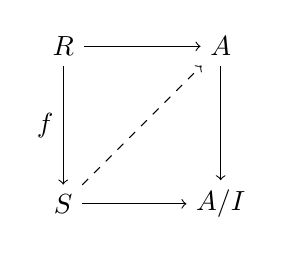
\begin{tikzpicture}
                \node (R) at (0, 1) {$R$};
                \node (S) at (0, -1) {$S$};
                \node (A) at (2, 1) {$A$};
                \node (AI) at (2, -1) {$A/I$};
                \draw[->] (R) -- node[left]{$f$} (S);
                \draw[->] (S) -- (AI);
                \draw[->] (R) -- (A);
                \draw[->] (A) -- (AI);
                \draw[->, dashed] (S) -- (A);
            \end{tikzpicture}
        \end{gather*}
        In other words, formally \'etale morphisms have the unique left lifting property with respect to infinitesimal thickenings. Saying that $f:R\rightarrow S$ is formally smooth (resp.~formally unramified) means that there exists at least (resp.~at most) one lift.
    }
    \begin{remark}[Topological rings]
        The previous definition can be generalized to \textit{topological rings} $R$ and $S$. In this case $A$ ranges over discrete algebras and all morphisms are taken to be continuous morphisms.
    \end{remark}

    \newdef{Completion\footnotemark}{\index{completion!of rings}\label{algebra:ring_completion}\index{formal!completion}\index{adic}
        \footnotetext{This form of ring completion is sometimes called the \textbf{formal completion} or \textbf{adic completion}.}
        Consider a commutative ring $R$ together with a proper ideal $I$. The completion $\widehat{R}$ of $R$ with respect to $I$ is the inverse limit $\varprojlim_{n\in\mathbb{N}}(R/I^n)$.
    }
    \begin{property}[Adic topology]\index{topology!adic}\index{Krull!topology}
        When the filtration ends in the trivial ideal, for example when $R$ is a Noetherian local ring, the completion $\widehat{R}$ is a topological ring (see \cref{chapter:topology}). The \textbf{Krull topology} or \textbf{$I$-adic topology} is the topology for which a basis of $0$ is given by the powers of $I$.
    \end{property}

    \begin{example}
        The completion of $R[x]$ with respect to $(x)$ is given by the ring of formal power series $R[[x]]$. In general one can think of these completions as containing (formal) \textit{Taylor series expansions}.
    \end{example}

\subsection{Modules}

    \newdef{$R$-module}{\index{module!over a ring}\label{algebra:module}
        Let $(R,+,\cdot)$ be a ring. An Abelian group $(M,\oplus)$ is said to be a left $R$-module if there exists a left (monoid) action $\triangleright:(R,\cdot)\times M\rightarrow M$ that satisfies the following axioms:
        \begin{enumerate}
            \item\textbf{Left distributivity}: $r\triangleright(m\oplus n) = r\triangleright m\oplus r\triangleright n$ for all $r\in R$ and $m,n\in M$.
            \item\textbf{Right distributivity}: $(r+s)\triangleright m = r\triangleright m \oplus s\triangleright m$ for all $r,s\in R$ and $m\in M$.
        \end{enumerate}
        These conditions make sure that both the additive structure $(R,+)$ and the group structure $(M,\oplus)$ are compatible with the action of $(R,\cdot)$. Due to these compatibility conditions one can identify $\cdot\sim\triangleright$ and $+\sim\oplus$ without confusion.
    }
    \begin{remark}[\difficult{Categorical perspective}]
        The definition of a ring can be defined more concisely in categorical terms. Recall the definition of an algebra over a monad (\cref{cat:algebra_monad}). Modules over a monoid object $A$ are defined as algebras over the monad $A\otimes-$. A ring $R$ is a monoid object in the category $\mathbf{Ab}$ of Abelian groups. So a module $M$ over $R$ consists of a morphism $\alpha:R\otimes M\rightarrow M$ satisfying the algebra axioms. The distributivity laws come for free since $\alpha$ is a morphism in $\mathbf{Ab}$ and, hence, is bilinear (in both arguments).
    \end{remark}
    \newadef{$R$-module}{
        The above two formulations can be restated similar to that of group modules (\cref{group:module}). Consider the Abelian group $(M,\oplus)$. Its endomorphism set $\End(M,\oplus)$ can be given the structure of a ring where the addition is induced by that on $M$ and the multiplication is given by composition. A left $R$-module structure is then simply a ring morphism $R\rightarrow\End(M,\oplus)$.
    }

    \newdef{Free module}{\index{free!module}\index{basis}
        An $R$-module $M$ that admits a \textbf{basis}, i.e.~there exists a set $\{x_i\}_{i\in I}$, where $I$ can be infinite, such that:
        \begin{enumerate}
            \item Every element $m\in M$ can be written as a linear combination $\sum_{j\in J_m}r_jx_j$, where $J_m\subseteq I$ is finite.
            \item The set $\{x_i\}_{i\in I}$ is linearly independent in the sense that
                \begin{gather}
                    \sum_{j\in J\subseteq I}r_jx_j=0\implies\forall j\in J:r_j=0.
                \end{gather}
        \end{enumerate}
    }
    \begin{example}[Dual numbers]\index{dual!numbers}
        Let $R$ be a ring. The $R$-algebra of dual numbers, often denoted by $R[\varepsilon]$, is defined as the free $R$-module with basis $\{1,\varepsilon\}$ subject to the relation $\varepsilon^2 = 0$.
    \end{example}

    \begin{property}[Division rings]\index{division!ring}\label{algebra:module_basis}
        For a general $R$-module the existence of a basis is not guaranteed unless $R$ is a \textit{division ring}. (See \cref{linalgebra:hamel_basis} for more information.)
    \end{property}
    \begin{result}
        Since every field is in particular a division ring, the existence of a basis follows from the above property for $R$-modules.
    \end{result}

    \newdef{Projective module}{\index{projective!module}
        A module $P$ that can be expressed as
        \begin{gather}
            P\oplus M=F\,,
        \end{gather}
        where $M$ is a module and $F$ is a free module, i.e.~$P$ is projective if it is a direct sumand of a free module.
    }

    \begin{theorem}[Nakayama lemma\footnotemark]\index{Nakayama lemma}\index{Krull--Azumaya}\label{algebra:nakayama}
        \footnotetext{Also called the \textbf{Krull--Azumaya lemma}.}
        Consider a commutative ring $R$. If $I\subset R$ is an ideal and $M$ a finitely-generated $R$-module such that $IM=M$, there exists an element $r\in R$ with $r=1$ in $R/I$ such that $rM=0$.
    \end{theorem}
    The following corrolary is also often called Nakayama's lemma:
    \begin{result}
        If $M$ is a finitely-generated $R$-module and $J(R)M=M$, then $M=0$.
    \end{result}
    \begin{result}
        If $M$ is a finitely-generated $R$-module and there exist elements $m_1,\ldots,m_k\in M$ whose image in $M/J(R)M$ generate this quotient, the elements generate $M$.
    \end{result}

\subsection{Semisimplicity}\index{semisimple!module}

    \newdef{Simple module}{\index{simple!module}
        A module over a ring that contains no nontrivial submodules. A module is said to be \textbf{semisimple} if it admits a decomposition as a direct sum of simple modules. A ring is said to be semisimple if it is semisimple as a module over itself.
    }
    \begin{property}[Jacobson radical]
        A ring is semisimple if and only if it is Artinian and if its Jacobson radical (\cref{algebra:jacobson_radical}) vanishes.
    \end{property}

    \begin{theorem}[Artin--Wedderburn]\index{Artin--Wedderburn}\label{algebra:artin_wedderburn}
        Every semisimple ring is isomorphic to a direct sum of matrix rings over division rings $D_i$ with multiplicity $n_i$. Furthermore, the integers $D_i$ and $n_i$ are unique (up to a permutation of the indices).
    \end{theorem}

\section{\difficult{Galois theory}}\index{Galois!theory}

\subsection{Polynomials}

    \newdef{Polynomial ring}{\index{poly-!nomial}\index{indeterminate}
        Let $R$ be a (commutative unital) ring and consider a set $X$. The polynomial ring on the \textbf{indeterminates} $X$ is defined as the free commutative $R$-algebra on $X$. Often, $X$ will be a finite set: $R[X]\equiv R[x_1,\ldots,x_n]$.
    }

    \begin{theorem}[Hilbert's basis theorem]\index{Hilbert!basis theorem}
        If a ring is Noetherian (\cref{algebra:noetherian_ring}), any polynomial ring with finitely many indeterminates over it is also Noetherian.
    \end{theorem}

    \newdef{Irreducible polynomial}{\index{irreducible!polynomial}
        A polynomial that cannot be factorized as the product of two nonconstant polynomials. Over a field, a polynomial is irreducible if and only if the ideal it generates is maximal.
    }

    \newdef{Degree}{\index{degree!of polynomial}
        The degree of a polynomial $f$ is equal to the largest integer $d\in\mathbb{N}$ for which $f$ contains a monomial $x_1^{i_1}\cdots x_n^{i_n}$ such that $i_1+\cdots+i_n=d$. It is denoted by $\deg(f)$.
    }
    \newdef{Monic polynomial}{\index{monic}
        A polynomial for which the highest degree term has coefficient $1$.
    }

    \newdef{Split}{\index{split}\index{root}
        A polynomial $f\in R[x]$ is said to split (over $R$) if it can be factorized as a product of linear factors, i.e.~there exist elements $\lambda,r_1,\ldots r_n$ such that
        \begin{gather}
            f = \lambda(x-r_1)\cdots(x-r_n)\,,
        \end{gather}
        where $n=\deg(f)$. The numbers $r_i\in R$ are called the \textbf{roots} of the polynomial.
    }

    \begin{theorem}[Fundamental theorem of algebra]\index{fundamental theorem!of algebra}\label{alggeom:fundamental_theorem_of_algebra}
        Consider a $\mathbb{C}$-valued polynomial of degree $\geq 1$. It has at least one root in $\mathbb{C}$.
    \end{theorem}
    \begin{result}
        If $f\in \mathbb{C}[x]$ is a monic polynomial with $\deg(f)\geq1$, it can be factorized as follows:
        \begin{gather*}
            f(x) = \prod_{i=1}^k(x-a_i)^{n_i},
        \end{gather*}
        where $a_1,\ldots, a_k\in\mathbb{C}$ and $n_1,\ldots,n_k\in\mathbb{N}$.
    \end{result}

    \begin{formula}[Vieta]\index{Vieta}
        Consider a polynomial of degree $n$. By the fundamental theorem of algebra, this polynomial has $n$ complex roots. Vieta's formulas relate the coefficients of the polynomial to its roots $r_i$:
        \begin{gather}
            \sum_{1\leq i_1\leq\ldots\leq i_k\leq n}\ \prod_{j=1}^kr_{i_j} = (-1)^k\frac{a_{n-k}}{a_n}\,,
        \end{gather}
        where $k\leq n$. For $k=1$ and $k=n$, this gives the well-known sum and product formulas:
        \begin{align}
            r_1+r_2+\cdots+r_n &= -\frac{a_{n-1}}{a_n}\,,\\
            r_1r_2\cdots r_n &= (-1)^n\frac{a_0}{a_n}\,.
        \end{align}
    \end{formula}
    \begin{example}
        For quadratic polynomials
        \begin{gather}
            f(x) = ax^2+bx+c\,,
        \end{gather}
        one recovers the following well-known formulas:
        \begin{align}
            r_1+r_2 &= -\frac{b}{a},\\
            r_1r_2 &= \frac{c}{a}\,.
        \end{align}
    \end{example}

\subsection{Field extensions}

    \newdef{Field extension}{\index{field!extension}\label{algebra:field_extension}
        Let $K$ be a field. A field extension of $K$ is a field $L$ such that $K\subseteq L$ and such that the operations of $K$ are the restrictions of those in $L$.
    }
    \begin{notation}
        A field extension $L$ of $K$ is often denoted by $L/K$.
    \end{notation}

    \begin{notation}[Generation]\index{simple!extension}
        Consider a field extension $L/K$ together with a subset $X\subseteq L$. The smallest field extension of $K$ that contains $X$ is denoted by $K(X)$. $L$ is said to be \textbf{simple} if $L=K(a)$ for some $a\in L$.
    \end{notation}

    \newdef{Degree}{\index{degree!of field extension}\index{extension!finite}
        If $L/K$ is a field extension, $L$ can be given the structure of a $K$-\textit{vector space} (see \cref{linalgebra:vector_space}). The dimension of this vector space is called the degree of the extension $K$. It is often denoted by $[L:K]$. If the degree is finite, the extension is also said to be \textbf{finite}.
    }

    The following property is very similar to the tower rule for finite groups (\cref{group:tower_rule_groups}).
    \begin{property}[Tower property]\index{tower law}
        Consider two field extensions $M/L$ and $L/K$.
        \begin{gather}
            [M:K]=[M:L][L:K]
        \end{gather}
    \end{property}
    \sremark{Galois theory will show that this is no mere coincidence.}

    \newdef{Number field}{\index{number!field}
        A finite extension of the rational numbers $\mathbb{Q}$.
    }

\subsection{Algebraicity}\label{section:algebraic_numbers}

    \newdef{Transcendental element}{\index{transcendental}\index{algebraic}
        Consider a field extension $L/K$. An element $x\in L$ for which there exist no nontrivial polynomials $p\in K[x]$ such that $p(x)=0$, is said to be transcendental, otherwise it is said to be \textbf{algebraic}.
    }

    \newdef{Algebraic dependence}{
        Consider a commutative ring $R$ and a subring $S\subset R$. An element $r\in R$ is said to be algebraically dependent on $S$ if it is the root of a polynomial in $S[x]$. If $r$ is the root of a monic polynomial in $S[x]$, it is said to be \textbf{integrally dependent} on $S$.
    }
    \begin{remark}
        Since every nonzero element in a field is invertible, one can always turn a general polynomial into a monic polynomial. Hence, over a field, the concepts of algebraic and integral dependence coincide.
    \end{remark}

    \newdef{Algebraic extension}{\index{extension!algebraic}
        An extension $L/K$ such that every element of $L$ is algebraic over $K$.
    }

    \begin{property}
        Every finite extension is algebraic.
    \end{property}

    \newdef{Algebraic closure}{\index{algebraic!closure}
        A field is said to be \textbf{algebraically closed} if every polynomial over it has a root. This implies that every polynomial splits. An algebraic closure of a field $K$ is an algebraic extension $\overline{K}/K$ such that $\overline{K}$ is algebraically closed.
    }
    \newdef{Splitting field}{\index{splitting field}\label{algebra:splitting_field}
        Consider a field $K$ and a polynomial $f\in K[x]$. The smallest field extension of $K$ over which $f$ splits is called the splitting field of $f$.
    }
    \begin{property}
        A splitting field of a polynomial of degree $n$ has degree at most $n!$.
    \end{property}
    \begin{example}
        \Cref{alggeom:fundamental_theorem_of_algebra} implies that $\mathbb{C}$ is an algebraic closure of $\mathbb{R}$. In fact, it is also the splitting field over $\mathbb{R}$.
    \end{example}

    \newdef{Minimal polynomial}{\index{minimal!polynomial}\index{evaluation}\label{algebra:minimal_polynomial}
        Consider a field extension $L/K$ with an element $a\in L$ that is algebraic over $K$. The monic polynomial $f^a\in K[x]$ of lowest order such that $f^a(a)=0$ is called the minimal polynomial of $a$. This polynomial is obtained as the generator\footnote{Polynomial rings in one variable are PIDs, so the kernel ideal admits a generator.} of the kernel ideal of the \textbf{evaluation morphism}
        \begin{gather}
            K[x]\rightarrow L:f\mapsto f(a)\,.
        \end{gather}
    }
    \begin{property}\label{algebra:minimal_polynomial_divisor}
        Let $f^a$ be the minimal polynomial of an algebraic element $a\in L$. If $f(a)=0$ for some polynomial $f\in K[x]$, the minimal polynomial $f^a$ divides $f$.
    \end{property}
    \begin{result}
        The minimal polynomial of an algebraic element is irreducible.
    \end{result}

    \begin{property}
        Consider two fields $K,L$ together with an element $a\in L$. The `polynomial ring' $K[a]$, the image of the evaluation morphism, coincides with $K(a)$ if and only if $a$ is algebraic over $K$.
    \end{property}

    \newdef{Separable element}{\index{separable}
        An element $a\in\overline{K}$ of an algebraic closure $\overline{K}/K$ is said to be separable (over $K$) if the minimal polynomial $f^\alpha\in K[x]$ is separable, i.e.~has no multiple zeros. A subextension $L\subset\overline{K}$ is said to be separable if every element of $L$ is separable over $K$.
    }
    \newdef{Separable closure}{\index{separable!closure}\label{algebra:separable_closure}
        Let $K$ be a field with algebraic closure $\overline{K}$. The separable closure $K_S$ is defined as follows:
        \begin{gather}
            K_S := \{x\in\overline{K}\mid x\text{ is separable over }K\}\,.
        \end{gather}
    }
    \begin{example}[Separable splitting field]
        The splitting field of a separable polynomial is separable.
    \end{example}

    \newdef{Perfect field}{\index{perfect!field}
        A field $K$ satisfying any of the following equivalent statements:
        \begin{enumerate}
            \item Every irreducible polynomial over $K$ is separable.
            \item Every algebraic extension of $K$ is separable.
            \item Every finite extension of $K$ is separable.
            \item The separable closure $K_S$ is algebraically closed.
        \end{enumerate}
    }
    \begin{example}
        All finite fields and fields of characteristic zero are perfect.
    \end{example}
    \begin{result}
        For a perfect field, the algebraic closure and separable closure coincide.
    \end{result}

    \newdef{Normal extension}{\index{extension!normal}
        A field extension $L/K$ with $L\subseteq\overline{K}$ is said to be \textbf{normal} if every irreducible polynomial in $K[x]$ that has a root in $L$ splits over $L$.
    }
    \begin{property}
        A field extension is normal if and only if it is the splitting field for some set of polynomials. Moreover, it is finite normal if and only if it is the splitting field of a single polynomial.
    \end{property}

    \newdef{Normal closure}{\index{normal!closure}
        Consider a field extension $L/K$. The normal closure of $L$ is the smallest normal extension of $L$ over $K$.
    }

\subsection{Galois extensions}

    \newdef{Galois extension}{\index{Galois!extension}\index{Krull!topology}\index{group!profinite}
        An algebraic field extension $L/K$ such that there exists a subgroup $G\subseteq\Aut(L)$ satisfying
        \begin{gather}
            K\cong L^G\,,
        \end{gather}
        where $L^G$ denotes the set of $G$-invariants of $L$. This group, often denoted by $\mathrm{Gal}(L/K)$, is called the \textbf{Galois group} of the extension. If $L$ is the splitting field of a polynomial $f\in K[x]$, the Galois group is sometimes denoted by $\mathrm{Gal}(f)$.

        When $L/K$ is finite, the Galois group is a finite group and, hence, can simply be endowed with the discrete topology. However, when the extension is not finite, one should endow the group with a topology. The \textbf{Krull topology} is defined as the \textit{profinite topology} (see \cref{topology:profinite_group}) with respect to all finite subgroups of $\mathrm{Gal}(L/K)$.\footnote{One can show that every \textit{profinite group} arises as a Galois group for some field extension.}
    }

    \begin{property}
        Consider a field extension $L/K$. The following statements are equivalent:
        \begin{itemize}
            \item $L$ is a Galois extension.
            \item $L$ is algebraic, normal and separable over $K$.
        \end{itemize}
    \end{property}
    \begin{property}
        A finite extension $L/K$ is Galois if and only if $|\mathrm{Gal}(L/K)|=[L:K]$.
    \end{property}

    \begin{theorem}[Fundamental theorem of Galois theory]\index{fundamental theorem!of Galois theory}
        Consider a Galois extension $L/K$. The intermediate field extensions $K'/K$ are in bijection with the closed subgroups of $\mathrm{Gal}(L/K)$.
    \end{theorem}
    \begin{property}
        Consider a subgroup $H\subset\mathrm{Gal}(L/K)$. The correspondence in the fundamental theorem has the following properties:
        \begin{itemize}
            \item $L/L^H$ is Galois.
            \item If $H$ is open, $L^H/K$ is finite.
            \item If $H$ is normal, $L^H/K$ is Galois with $\mathrm{Gal}\left(L^H/K\right)\cong\mathrm{Gal}(L/K)/H$.
        \end{itemize}
    \end{property}

\subsection{Radicals}

    \newdef{Radical extension}{\index{extension!radical}\index{radical|seealso{extension}}
        A simple radical extension $L/K$ is a simple extension $L=K(a)$ such that $a^n=b$ for some $b\in K$ and $n\in\mathbb{N}_0$. A radical extension or radical series is a finite sequence of simple radical extensions.
    }

    \begin{property}
        If $L/K$ is radical and $K'$ is an intermediate field extension, $\Aut(K'/K)$ is solvable.
    \end{property}

    \begin{theorem}[Galois]
        A polynomial $f\in K[x]$, where $\mathrm{char}(K)$ does not divide $\deg(f)$, can be solved by radicals if and only if its Galois group $\mathrm{Gal}(f)$ is solvable (\cref{group:solvable}).
    \end{theorem}

    \todo{COMPLETE}

\subsection{Nullstellensatz}\index{Nullstellensatz}

    For the geometric incarnation, see \cref{chapter:alggeom}.

    \begin{theorem}[Weak Nullstellensatz]
        Let $K$ be an algebraically closed field and consider the polynomial ring $R=K[x_1,\ldots,x_n]$. An ideal $I\subset R$ is maximal if and only if it is of the form \[(x_1-a_1,\ldots,x_n-a_n)\] with $a_i\in K$ for all $i\leq n$.
    \end{theorem}
    \begin{result}
        There exists a bijection between $K^n$ and the set of maximal ideals of $K[x_1,\ldots,x_n]$.
    \end{result}
    \begin{result}
        Consider a collection of polynomials $\{f_i\}_{i\in I}\subset K[x_1,\ldots,x_n]$. If these polynomials do not have a common root, the ideal they generate is the unit ideal.
    \end{result}

    \todo{COMPLETE}
% \input{Math/Set/CategoryTheory}
% \chapter{\difficult{Higher-dimensional Algebra}}\label{chapter:hda}

    The main reference for this chapter is a series of eponymous papers~\citep{baez_higher-dimensional_2003, baez_higher-dimensional_2003-1}. For Kapranov-Voevodsky 2-vector spaces, the reader is referred to the original paper by~\citet{kapranov_2-categories_1994}. References for the section on Berezin calculus are~\citet{losev_berezin_2007, choquet-bruhat_analysis_2000}. The section about higher Lie theory is mainly based on~\citet{fiorenza_introduction_2004}. For fusion and modular categories, the main reference is~\citet{etingof_tensor_2016}.

    \minitoc

\section{Monoidal categories}\label{section:monoidal_categories}

    \newdef{Monoidal category}{\index{monoidal!category}\index{tensor product}\label{cat:monoidal_category}
        A category $\mathbf{C}$ equipped with a bifunctor
        \begin{gather}
            -\otimes -:\mathbf{C}\times\mathbf{C}\rightarrow\mathbf{C}\,,
        \end{gather}
        called the \textbf{tensor product} or \textbf{monoidal product}, a distinct object $\mathbf{1}$, called the \textbf{(monoidal) unit}, and the following three natural isomorphisms, called the \textbf{coherence maps}:
        \begin{itemize}
            \item\textbf{Associator}: $\alpha_{x,y,z}:(x\otimes y)\otimes z\cong x\otimes(y\otimes z)$,
            \item\textbf{Left unitor}: $\lambda_x:\mathbf{1}\otimes x\cong x$, and
            \item\textbf{Right unitor}: $\rho_x:x\otimes\mathbf{1}\cong x$.
        \end{itemize}
        These natural transformations are required make the \textbf{triangle} and \textbf{pentagon} diagrams in \cref{fig:triangle_diagram} and \cref{fig:pentagon_diagram}, respectively, commute. A monoidal category for which the associator and the unitors are identity transformations is often said to be \textbf{strict}.

        \begin{figure}[ht!]
            \centering
            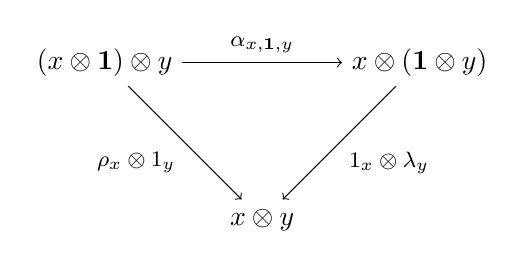
\begin{tikzpicture}
                \node (1) at (0, 0) {$(x\otimes\mathbf{1})\otimes y$};
                \node (2) at (4, 0) {$x\otimes(\mathbf{1}\otimes y)$};
                \node (3) at (2, -2) {$x\otimes y$};
                \draw[->] (1) -- node[above]{\footnotesize$\alpha_{x,\mathbf{1},y}$} (2);
                \draw[->] (1) -- node[below left]{\footnotesize$\rho_x\otimes\mathbbm{1}_y$} (3);
                \draw[->] (2) -- node[below right]{\footnotesize$\mathbbm{1}_x\otimes\lambda_y$} (3);
            \end{tikzpicture}
            \caption{Triangle diagram.}
            \label{fig:triangle_diagram}
        \end{figure}
    }

    \begin{figure}[ht!]
        \centering
        \begin{tikzpicture}
            \node (1) at (0, 0) {$\bigl((w\otimes x)\otimes y\bigr)\otimes z$};
            \node (2) at (6, 0) {$\bigl(w\otimes(x\otimes y)\bigr)\otimes z$};
            \node (3) at (-2, -3) {$(w\otimes x)\otimes(y\otimes z)$};
            \node (4) at (8, -3) {$w\otimes\bigl((x\otimes y)\otimes z\bigr)$};
            \node (5) at (3, -6) {$w\otimes\bigl(x\otimes(y\otimes z)\bigr)$};
            \draw[->] (1) -- node[above]{\small$\alpha_{w,x,y}\otimes\mathbbm{1}_z$} (2);
            \draw[->] (1) -- node[above left]{\small$\alpha_{w\otimes x,y,z}$} (3);
            \draw[->] (3) -- node[below left]{\small$\alpha_{w,x,y\otimes z}$} (5);
            \draw[->] (2) -- node[above right]{\small$\alpha_{w,x\otimes y,z}$} (4);
            \draw[->] (4) -- node[below right]{\small$\mathbbm{1}_w\otimes\alpha_{x,y,z}$} (5);
        \end{tikzpicture}
        \caption{Pentagon diagram.}
        \label{fig:pentagon_diagram}
    \end{figure}

    \begin{example}[Cartesian category]\label{cat:semicartesian}
        A monoidal category where the monoidal product is given by the ordinary product (\cref{cat:product}). If the monoidal product is not the ordinary product, but the monoidal unit is still terminal, the category is said to be \textbf{semicartesian}.
    \end{example}

    \newdef{Scalar}{\index{scalar}
        In a monoidal category, the scalars are defined as the endomorphisms $\mathbf{1}\rightarrow\mathbf{1}$. The set of scalars forms a commutative monoid.
    }
    \begin{property}
        Every scalar $s:\mathbf{1}\rightarrow\mathbf{1}$ induces a natural transformation $s:\mathbbm{1}_{\mathbf{C}}\Rightarrow\mathbbm{1}_{\mathbf{C}}$ with components
        \begin{gather}
            s_x:x\cong\mathbf{1}\otimes x\overset{s\otimes\mathbbm{1}_x}{\longrightarrow}\mathbf{1}\otimes x\cong x\,.
        \end{gather}
        For every morphism $f\in\mathrm{hom}(\mathbf{C})$, the naturality square $f\circ s_x=s_y\circ f$ alo defines a morphism $s\diamond f$ that is equivalently given by $\rho_y\circ(f\otimes s)\circ\rho^{-1}_x$ (one could have used the left unitors as well). These morphisms satisfy the following well-known rules of scalar multiplication from linear algebra:
        \begin{itemize}
            \item $s\diamond(s'\diamond f) = (s\circ s')\diamond f$,
            \item $(s\diamond f)\circ(s'\diamond g) = (s\circ s')\diamond(f\circ g)$, and
            \item $(s\diamond f)\otimes(s'\diamond g) = (s\circ s')\diamond(f\otimes g)$.
        \end{itemize}
    \end{property}

    \newdef{Weak inverse}{\index{weak!inverse}
        Let $(\mathbf{C},\otimes,\mathbf{1})$ be a monoidal category. An object $y\in\ob{C}$ is called a weak inverse of an object $x\in\ob{C}$ if it satisfies $x\otimes y\cong\mathbf{1}$.
    }
    \begin{remark}
        One can show that the existence of a one-sided weak inverse (as in the definition above) implies that it is in fact a two-sided weak inverse, i.e.~$y\otimes x\cong\mathbf{1}$ also holds.
    \end{remark}

    \begin{theorem}[MacLane's coherence theorem]\index{MacLane!coherence theorem}\index{coherence|seealso{MacLane}}
        Consider two functors $\func{F,G}{A}{B}$ between two monoidal categories $\mathbf{A},\mathbf{B}$. Any two natural transformations $\eta,\varepsilon:F\Rightarrow G$, constructed solely from the associator and the unitors, coincide.
    \end{theorem}

\subsection{Braided categories}

    \newdef{Braided monoidal category}{\index{braiding}
        A monoidal category $(\mathbf{C},\otimes,\mathbf{1})$ equipped with a natural isomorphism
        \begin{gather}
            \sigma_{x,y}:x\otimes y\cong y\otimes x
        \end{gather}
        that makes the two \textbf{hexagon} diagrams~\ref{fig:hexagon_diagrams1} and~\ref{fig:hexagon_diagrams2} commute for all $x,y,z\in\ob{C}$. The isomorphism $\sigma$ is called the \textbf{braiding} (morphism).
        \begin{figure}[ht!]
            \centering
            \begin{subfigure}[b]{0.49\textwidth}
                \centering
                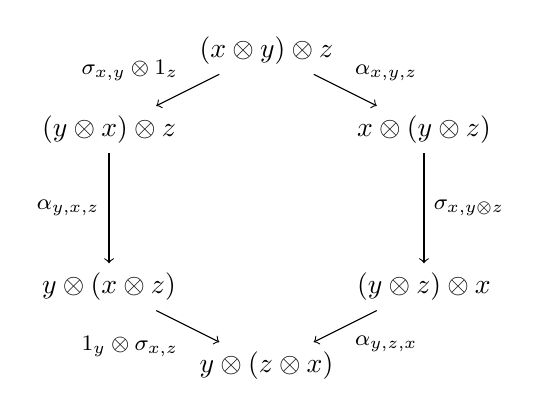
\begin{tikzpicture}
                    \node (1) at (0, 0) {$(x\otimes y)\otimes z$};
                    \node (2) at (-2, -1) {$(y\otimes x)\otimes z$};
                    \node (3) at (2, -1) {$x\otimes(y\otimes z)$};
                    \node (4) at (-2, -3) {$y\otimes(x\otimes z)$};
                    \node (5) at (2, -3) {$(y\otimes z)\otimes x$};
                    \node (6) at (0, -4) {$y\otimes(z\otimes x)$};
                    \draw[->] (1) -- node[above left]{\footnotesize$\sigma_{x,y}\otimes\mathbbm{1}_z$} (2);
                    \draw[->] (1) -- node[above right]{\footnotesize$\alpha_{x,y,z}$} (3);
                    \draw[->] (2) -- node[left]{\footnotesize$\alpha_{y,x,z}$} (4);
                    \draw[->] (3) -- node[right]{\footnotesize$\sigma_{x,y\otimes z}$} (5);
                    \draw[->] (4) -- node[below left]{\footnotesize$\mathbbm{1}_y\otimes\sigma_{x,z}$} (6);
                    \draw[->] (5) -- node[below right]{\footnotesize$\alpha_{y,z,x}$} (6);
                \end{tikzpicture}
                \caption{Hexagon diagram 1.}
                \label{fig:hexagon_diagrams1}
            \end{subfigure}
            \begin{subfigure}[b]{0.49\textwidth}
                \centering
                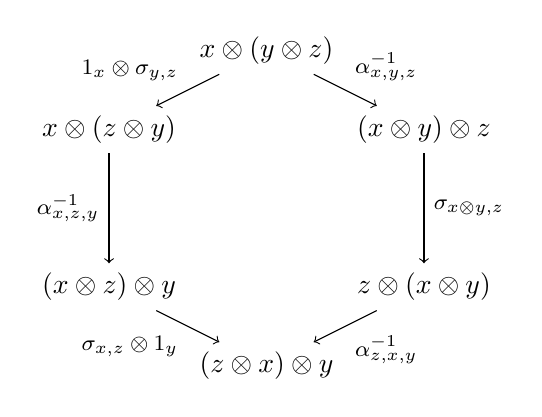
\begin{tikzpicture}
                    \node (1) at (0, 0) {$x\otimes(y\otimes z)$};
                    \node (2) at (-2, -1) {$x\otimes(z\otimes y)$};
                    \node (3) at (2, -1) {$(x\otimes y)\otimes z$};
                    \node (4) at (-2, -3) {$(x\otimes z)\otimes y$};
                    \node (5) at (2, -3) {$z\otimes(x\otimes y)$};
                    \node (6) at (0, -4) {$(z\otimes x)\otimes y$};
                    \draw[->] (1) -- node[above left]{\footnotesize$\mathbbm{1}_x\otimes\sigma_{y,z}$} (2);
                    \draw[->] (1) -- node[above right]{\footnotesize$\alpha^{-1}_{x,y,z}$} (3);
                    \draw[->] (2) -- node[left]{\footnotesize$\alpha^{-1}_{x,z,y}$} (4);
                    \draw[->] (3) -- node[right]{\footnotesize$\sigma_{x\otimes y,z}$} (5);
                    \draw[->] (4) -- node[below left]{\footnotesize$\sigma_{x,z}\otimes\mathbbm{1}_y$} (6);
                    \draw[->] (5) -- node[below right]{\footnotesize$\alpha^{-1}_{z,x,y}$} (6);
                \end{tikzpicture}
                \caption{Hexagon diagram 2.}
                \label{fig:hexagon_diagrams2}
            \end{subfigure}
            \caption{Hexagon diagram.}
            \label{fig:hexagon_diagrams}
        \end{figure}
    }
    \begin{property}[Yang--Baxter equation]\index{Yang--Baxter}
        The components $\sigma_{x,x}$ of a braiding satisfy the \textit{Yang--Baxter equation}. More generally, the braiding $\sigma$ satisfies the following equation for all objects $x,y,z\in\ob{C}$:
        \begin{gather}
            (\sigma_{y,z}\otimes\mathbbm{1}_x)\circ(\mathbbm{1}_y\otimes\sigma_{x,z})\circ(\sigma_{x,y}\otimes\mathbbm{1}_z) = (\mathbbm{1}_z\otimes\sigma_{x,y})\circ(\sigma_{x,z}\otimes\mathbbm{1}_y)\circ(\mathbbm{1}_x\otimes\sigma_{y,z})\,.
        \end{gather}
    \end{property}\index{Reidemeister move}
    \remark{When drawing the above equality using string diagrams, it can be seen that the Yang--Baxter equation corresponds to the invariance of string diagrams under a \textit{Reidemeister-III move}.\index{Reidemeister move}}

    \newdef{Symmetric monoidal category}{\label{cat:symmetric}
        A braided monoidal category where the braiding $\sigma$ satisfies
        \begin{gather}
            \sigma_{x,y}\circ\sigma_{y,x} = \mathbbm{1}_{x\otimes y}\,.
        \end{gather}
    }

\subsection{Monoidal functors}

    \begin{figure}[ht!]
        \centering
        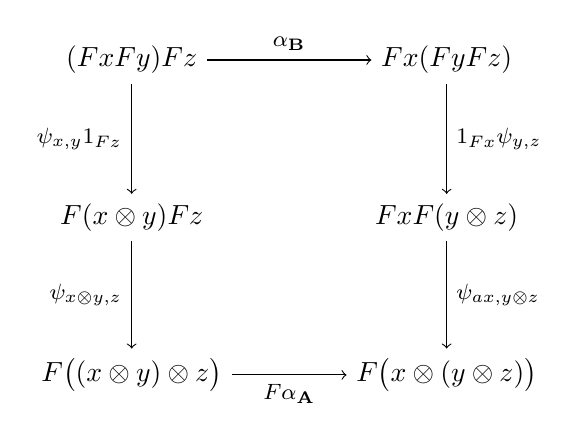
\begin{tikzpicture}
            \node (1) at (0, 0) {$(Fx\circledast Fy)\circledast Fz$};
            \node (2) at (4, 0) {$Fx\circledast(Fy\circledast Fz)$};
            \node (3) at (0, -2) {$F(x\otimes y)\circledast Fz$};
            \node (4) at (4, -2) {$Fx\circledast F(y\otimes z)$};
            \node (5) at (0, -4) {$F\bigl((x\otimes y)\otimes z\bigr)$};
            \node (6) at (4, -4) {$F\bigl(x\otimes(y\otimes z)\bigr)$};
            \draw[->] (1) -- node[above]{\footnotesize$\alpha_{\mathbf{B}}$} (2);
            \draw[->] (5) -- node[below]{\footnotesize$F\alpha_{\mathbf{A}}$} (6);
            \draw[->] (1) -- node[left]{\footnotesize$\psi_{x,y}\circledast\mathbbm{1}_{Fz}$} (3);
            \draw[->] (3) -- node[left]{\footnotesize$\psi_{x\otimes y,z}$} (5);
            \draw[->] (2) -- node[right]{\footnotesize$\mathbbm{1}_{Fx}\circledast\psi_{y,z}$} (4);
            \draw[->] (4) -- node[right]{\footnotesize$\psi_{ax,y\otimes z}$} (6);
        \end{tikzpicture}
        \caption{Monoidal functor.}
        \label{fig:monoidal_functor1}
    \end{figure}

    \newdef{Monoidal functor}{\index{monoidal!functor}\index{coherence!maps}
        Let $(\mathbf{A},\otimes,\mathbf{1}_{\mathbf{A}}),(\mathbf{B},\circledast,\mathbf{1}_{\mathbf{B}})$ be two monoidal categories. A functor $\func{F}{A}{B}$ is said to be monoidal if there exists:
        \begin{enumerate}
            \item a natural isomorphism $\psi_{x,y}:Fx\circledast Fy\Rightarrow F(x\otimes y)$ that makes the diagram in \cref{fig:monoidal_functor1} commute, and
            \item an isomorphism $\phi:\mathbf{1}_{\mathbf{B}}\rightarrow F\mathbf{1}_{\mathbf{A}}$ that makes the two diagrams in \cref{fig:unitality} commute.
        \end{enumerate}
        The maps $\psi$ and $\phi$ are also called \textbf{coherence maps} or \textbf{structure morphisms}.
    }

    \begin{figure}[ht!]
        \centering
        \begin{subfigure}[b]{0.49\textwidth}
            \centering
            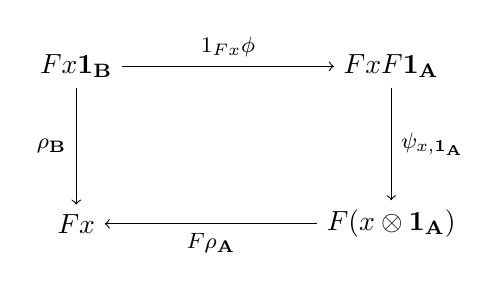
\begin{tikzpicture}
                \node (1) at (0, 0) {$Fx\circledast\mathbf{1}_{\mathbf{B}}$};
                \node (2) at (4, 0) {$Fx\circledast F\mathbf{1}_{\mathbf{A}}$};
                \node (3) at (0, -2) {$Fx$};
                \node (4) at (4, -2) {$F(x\otimes\mathbf{1}_{\mathbf{A}})$};
                \draw[->] (1) -- node[above]{\footnotesize$\mathbbm{1}_{Fx}\circledast\phi$} (2);
                \draw[<-] (3) -- node[below]{\footnotesize$F\rho_{\mathbf{A}}$} (4);
                \draw[->] (1) -- node[left]{\footnotesize$\rho_{\mathbf{B}}$} (3);
                \draw[->] (2) -- node[right]{\footnotesize$\psi_{x,\mathbf{1}_{\mathbf{A}}}$} (4);
            \end{tikzpicture}
        \end{subfigure}
        \begin{subfigure}[b]{0.49\textwidth}
            \centering
            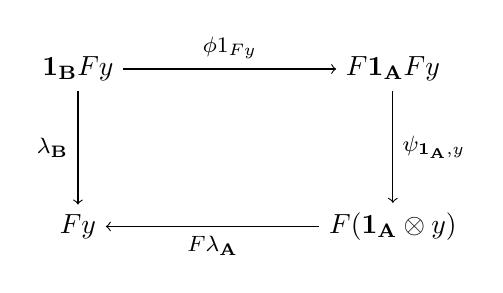
\begin{tikzpicture}
                \node (1) at (0, 0) {$\mathbf{1}_{\mathbf{B}}\circledast Fy$};
                \node (2) at (4, 0) {$F\mathbf{1}_{\mathbf{A}}\circledast Fy$};
                \node (3) at (0, -2) {$Fy$};
                \node (4) at (4, -2) {$F(\mathbf{1}_{\mathbf{A}}\otimes y)$};
                \draw[->] (1) -- node[above]{\footnotesize$\phi\circledast\mathbbm{1}_{Fy}$} (2);
                \draw[<-] (3) -- node[below]{\footnotesize$F\lambda_{\mathbf{A}}$} (4);
                \draw[->] (1) -- node[left]{\footnotesize$\lambda_{\mathbf{B}}$} (3);
                \draw[->] (2) -- node[right]{\footnotesize$\psi_{\mathbf{1}_{\mathbf{A}},y}$} (4);
            \end{tikzpicture}
        \end{subfigure}
        \caption{Unitality diagrams.}
        \label{fig:unitality}
    \end{figure}

    \begin{property}[Canonical unit]
        For every monoidal functor $F$, there exists a canonical isomorphism $\phi:\mathbf{1}_{\mathbf{B}}\rightarrow F\mathbf{1}_{\mathbf{A}}$ defined by the commutative diagram in \cref{fig:canonical_monoidal_isom}.

        \begin{figure}[ht!]
            \centering
            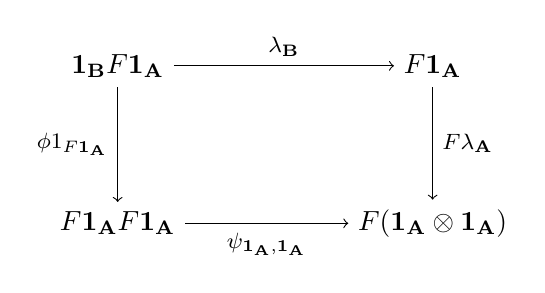
\begin{tikzpicture}
                \node (1) at (0, 0) {$\mathbf{1}_{\mathbf{B}}\circledast F\mathbf{1}_{\mathbf{A}}$};
                \node (2) at (4, 0) {$F\mathbf{1}_{\mathbf{A}}$};
                \node (3) at (0, -2) {$F\mathbf{1}_{\mathbf{A}}\circledast F\mathbf{1}_{\mathbf{A}}$};
                \node (4) at (4, -2) {$F(\mathbf{1}_{\mathbf{A}}\otimes\mathbf{1}_{\mathbf{A}})$};
                \draw[->] (1) -- node[above]{\footnotesize$\lambda_{\mathbf{B}}$} (2);
                \draw[->] (3) -- node[below]{\footnotesize$\psi_{\mathbf{1}_{\mathbf{A}}, \mathbf{1}_{\mathbf{A}}}$} (4);
                \draw[->] (1) -- node[left]{\footnotesize$\phi\circledast\mathbbm{1}_{F\mathbf{1}_{\mathbf{A}}}$} (3);
                \draw[->] (2) -- node[right]{\footnotesize$F\lambda_{\mathbf{A}}$} (4);
            \end{tikzpicture}
            \caption{Canonical unit isomorphism.}
            \label{fig:canonical_monoidal_isom}
        \end{figure}
    \end{property}

    \newdef{Lax monoidal functor}{\index{lax!monoidal functor}
        A monoidal functor for which the coherence maps are merely morphisms and not isomorphisms.
    }

    \newdef{Monoidal natural transformation}{
        A natural transformation $\eta$ between (lax) monoidal functors $(F,\psi,\phi_F)$ and $(G,\widetilde{\psi},\phi_G)$ that makes the diagrams in \cref{fig:monoidal_natural_transformation} commute.
        \begin{figure}[ht!]
            \centering
            \begin{subfigure}[b]{0.49\textwidth}
                \centering
                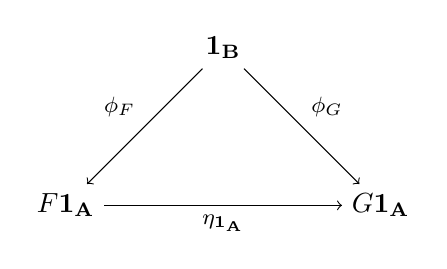
\begin{tikzpicture}
                    \node (1) at (0, 0) {$\mathbf{1}_{\mathbf{B}}$};
                    \node (2) at (-2, -2) {$F\mathbf{1}_{\mathbf{A}}$};
                    \node (3) at (2, -2) {$G\mathbf{1}_{\mathbf{A}}$};
                    \draw[->] (1) -- node[above left]{\footnotesize$\phi_F$} (2);
                    \draw[->] (1) -- node[above right]{\footnotesize$\phi_G$} (3);
                    \draw[->] (2) -- node[below]{\footnotesize$\eta_{\mathbf{1}_{\mathbf{A}}}$} (3);
                \end{tikzpicture}
            \end{subfigure}
            \begin{subfigure}[b]{0.49\textwidth}
                \centering
                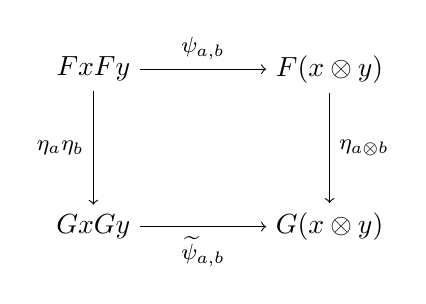
\begin{tikzpicture}
                    \node (1) at (0, 0) {$Fx\circledast Fy$};
                    \node (2) at (3, 0) {$F(x\otimes y)$};
                    \node (3) at (0, -2) {$Gx\circledast Gy$};
                    \node (4) at (3, -2) {$G(x\otimes y)$};
                    \draw[->] (1) -- node[above]{\footnotesize$\psi_{a,b}$} (2);
                    \draw[->] (3) -- node[below]{\footnotesize$\widetilde{\psi}_{a,b}$} (4);
                    \draw[->] (1) -- node[left]{\footnotesize$\eta_a\circledast\eta_b$} (3);
                    \draw[->] (2) -- node[right]{\footnotesize$\eta_{a\otimes b}$} (4);
                \end{tikzpicture}
            \end{subfigure}
            \caption{Monoidal natural transformation.}
            \label{fig:monoidal_natural_transformation}
        \end{figure}
    }

    \newdef{Monoidal equivalence}{\index{monoidal!equivalence}
        An equivalence of monoidal categories consisting of monoidal functors and monoidal natural isomorphisms.
    }
    \begin{theorem}[MacLane's strictness theorem]\index{MacLane!strictness theorem}
        Every monoidal category is monoidally equivalent to a strict monoidal category.
    \end{theorem}

\subsection{Closed categories}

    \newdef{Internal hom}{\index{internal!hom}\index{currying}\label{cat:internal_hom}
        Let $(\mathbf{M},\otimes,\mathbf{1})$ be a monoidal category. In this setting, one can generalize the \textit{currying} procedure, i.e.~the identification of maps $x\times y\rightarrow z$ with maps $x\rightarrow(y\rightarrow z)$. The internal hom-functor $\underline{\hom}$ is defined by the following natural isomorphism:
        \begin{gather}
            \mathbf{M}(x\otimes y,z)\cong\mathbf{M}\bigl(x,\underline{\hom}(y,z)\bigr).
        \end{gather}
        The existence of all internal homs is equivalent to the existence of a right adjoint to the tensor functor.
    }
    \begin{notation}
        The internal hom $\underline{\hom}(x,y)$ is also often denoted by $[x,y]$ (or $x\multimap y$). From now on, this convention will be followed (unless otherwise specified).
    \end{notation}
    \newdef{Closed monoidal category}{\index{closed!category}\index{Cartesian!closed}\label{cat:closed}
        A monoidal category that admits all internal homs. If the monoidal structure is induced by a (Cartesian) product structure, the category is often said to be \textbf{Cartesian closed}. A category for which all slice categories are Cartesian closed is said to be \textbf{locally Cartesian closed}.
    }
    \begin{property}
        A locally Cartesian closed category with a terminal object is Cartesian closed. Moreover, it is finitely complete. More generally, a locally Cartesian closed category has all pullbacks.
    \end{property}

    \newdef{Exponential object}{\index{exponential!object}\label{cat:exponential_object}
        In the case of Cartesian (monoidal) categories, the internal hom $[x,y]$ is called the exponential object. This object is often denoted by $y^x$.

        In Cartesian closed categories, a different, but frequently used, notation is $x\Rightarrow y$. However, this notation will not be used as it might be confused with the notation for \textit{2-morphisms}.
    }

    \newdef{Cartesian closed functor}{\index{Cartesian!closed}\label{cat:cartesian_closed_functor}
        A functor between Cartesian closed categories that preserves products and exponential objects. As such, it is the natural notion of functor between Cartesian closed categories.
    }
    \begin{property}[Frobenius reciprocity]\index{Frobenius!reciprocity}
        A functor $R$ between Cartesian closed categories that admits a left adjoint $L$ is Cartesian closed if and only if the natural transformation
        \begin{gather}
            L(y\times Rx)\rightarrow Ly\times x
        \end{gather}
        is a natural isomorphism.
    \end{property}

    \begin{property}[Global elements]\label{cat:internal_hom_property}
        The following isomorphism is natural in both $x,y\in\ob{M}$:
        \begin{gather}
            \mathbf{M}\bigl(\mathbf{1},[x,y]\bigr)\cong\mathbf{M}(x,y)\,.
        \end{gather}
        It is this relation that gives the best explanation for the term `internal hom'. One also immediately obtains the following natural isomorphism:
        \begin{gather}
            \mathbf{M}\bigl(x,[\mathbf{1},y]\bigr)\cong\mathbf{M}(x,y)\,.
        \end{gather}
        Because the Yoneda embedding is fully faithful, this implies that $[\mathbf{1},y]\cong y$. Although the global elements $\mathbf{M}(\mathbf{1},y)$ do not fully specify an object $y$, this does hold internally.
    \end{property}

    \begin{property}[Symmetry]\label{cat:internal_symmetry}
        Let $\mathbf{M}$ be a closed monoidal category. The definition of an internal hom can also be internalized, i.e.~there exists a natural isomorphism of the form
        \begin{gather}
            [x\otimes y,z]\cong[x,[y,z]]\,.
        \end{gather}
        Furthermore, if $\mathbf{M}$ is also symmetric, there exists an internal isomorphism of the form
        \begin{gather}
            [x,[y,z]]\cong[y,[x,z]]\,.
        \end{gather}
    \end{property}

    \newdef{Strong adjunction}{\index{adjunction!strong}
        Consider a monoidal category $\mathbf{M}$ together with two endofunctors $\func{L,R}{M}{M}$. These functors are said to form a strong adjunction if there exists a natural isomorphism
        \begin{gather}
            [Lx,y]\cong[x,Ry]\,.
        \end{gather}
        \Cref{cat:internal_hom_property} above implies that every strong adjunction is, in particular, an ordinary adjunction in the sense of \cref{section:adjunction}.
    }

\section{Enriched category theory}\label{section:enriched_category_theory}

    The following definition is due to \textit{B\'enabou}. It should represent the `ideal place in which to do category theory'.
    \newdef{Cosmos}{\index{cosmos}\label{cat:cosmos}
        A complete and cocomplete, closed symmetric monoidal category.
    }

    \newdef{Enriched category}{\index{category!enriched}
        Let $(\mathcal{V},\otimes,\mathbf{1})$ be a monoidal category. A $\mathcal{V}$-enriched category, also called a $\mathcal{V}$-category\footnote{Not to be confused with the notation for fibre categories (\cref{cat:fibre_category}).}, consists of the following elements:
        \begin{itemize}
            \item a collection of objects $\ob{C}$, and
            \item for every pair of objects $x,y\in\ob{C}$, an object $\mathbf{C}(x,y)\in\ob{\mathcal{V}}$ for which the following morphisms exist:
            \begin{enumerate}
                \item $\mathrm{id}_x:\mathbf{1}\rightarrow\mathbf{C}(x,x)$ giving the (enriched) identity morphism, and
                \item $\circ_{xyz}:\mathbf{C}(y,z)\otimes\mathbf{C}(x,y)\rightarrow\mathbf{C}(x,z)$ replacing the usual composition.
            \end{enumerate}
        \end{itemize}
        The associativity and unity properties are given by commutative diagrams for the $\mathrm{id}$ and $\circ$ morphisms together with the associators and unitors in $\mathcal{V}$.
    }

    \newdef{Change of base}{\index{change of base}\label{cat:change_of_base}
        Consider a monoidal functor $\func{F}{\mathcal{V}}{\mathcal{W}}$. This induces a change-of-base functor $F_*:\mathcal{V}\mathbf{Cat}\rightarrow\mathcal{W}\mathbf{Cat}$ by applying $F$ to every hom-object.
    }

    \newdef{Underlying category}{
        Given a $\mathcal{V}$-enriched category $\mathbf{C}$, the underlying category $\mathbf{C}_0$ is defined as follows:
        \begin{itemize}
            \item\textbf{Objects}: $\ob{C}$, and
            \item\textbf{Morphisms}: $\mathcal{V}\bigl(\mathbf{1},\mathbf{C}(x,y)\bigr)$,
        \end{itemize}
        where $\mathbf{1}$ is the monoidal unit in $\mathcal{V}$. This construction can be obtained as the functor $\mathcal{V}\mathbf{Cat}(\mathcal{I},-)$, where $\mathcal{I}$ is the one-object $\mathcal{V}$-category with $\mathcal{I}(\ast,\ast):=\mathbf{1}$.
    }
    \begin{property}[$\mathcal{V}$ as a $\mathcal{V}$-category]
        Consider a closed monoidal category $\mathcal{V}$. This category can be given the structure $\widetilde{\mathcal{V}}$ of a $\mathcal{V}$-category by taking the hom-objects to be the internal homs, i.e.~$\widetilde{\mathcal{V}}(x,y) := [x,y]$ for all $x,y\in\mathcal{V}$. \Cref{cat:internal_hom_property} then implies that there exists an isomorphism between the underlying category $\widetilde{\mathcal{V}}_0$ and the original category $\mathcal{V}$.
    \end{property}

    Given two $\mathcal{V}$-enriched categories, one can define suitable functors between them.
    \newdef{Enriched functor}{\index{functor}
        A $\mathcal{V}$-enriched functor $\func{F}{A}{B}$ consists of the following data:
        \begin{itemize}
            \item a function $F_0:\ob{A}\rightarrow\ob{B}$ (as for ordinary functors), and
            \item for every two objects $x,y\in\ob{A}$, a morphism $F_{x,y}:\mathbf{A}(x,y)\rightarrow\mathbf{B}(Fx,Fy)$ in $\mathcal{V}$.
        \end{itemize}
        These have to satisfy the `usual' composition and unit conditions.

        By extending \cref{cat:natural_end} using enriched ends, one obtains a definition of enriched natural transformations and, therefore, also a definition of enriched functor categories:
        \begin{gather}
            \label{cat:enriched_nat_end}
            \funccat{A}{B}(F,G) := \int_{x\in\mathbf{A}}\mathbf{B}(Fx,Gx)\,.
        \end{gather}
    }
    Given two $\mathcal{V}$-enriched functors $\func{F,G}{A}{B}$, one can also try to define $\mathcal{V}$-natural transformations by extending the usual definition of natural transformations (\cref{cat:natural}).
    \newdef{Enriched natural transformation}{\index{natural!transformation}
         An ordinary natural transformation consists of an $\ob{A}$-indexed family of morphism $\eta_x:Fx\rightarrow Gx$. This can also be interpreted as an $\ob{A}$-indexed family of morphisms $\eta_x:1\rightarrow\mathbf{B}(Fx,Gx)$ from the initial object (one-element set). By analogy, a $\mathcal{V}$-natural transformation is defined as an $\ob{A}$-indexed family of morphisms $\eta_x:\mathbf{1}\rightarrow\mathbf{B}(Fx,Gx)$ from the monoidal unit. The usual naturality square is replaced by the naturality hexagon in \cref{fig:v_naturality}.
    }

    The question then becomes how these two definitions are related. The end in \cref{cat:enriched_nat_end} comes equipped with a projection $\varepsilon_x:\funccat{A}{B}(F,G)\rightarrow\mathbf{B}(Fx,Gx)$. Precomposing this morphism with a morphism in the underlying category $\funccat{A}{B}_0$ exactly gives a $\mathcal{V}$-natural transformation. So, the underlying category of $\funccat{A}{B}$ is the ordinary category of $\mathcal{V}$-functors and $\mathcal{V}$-natural transformations.

     \begin{figure}
        \centering
        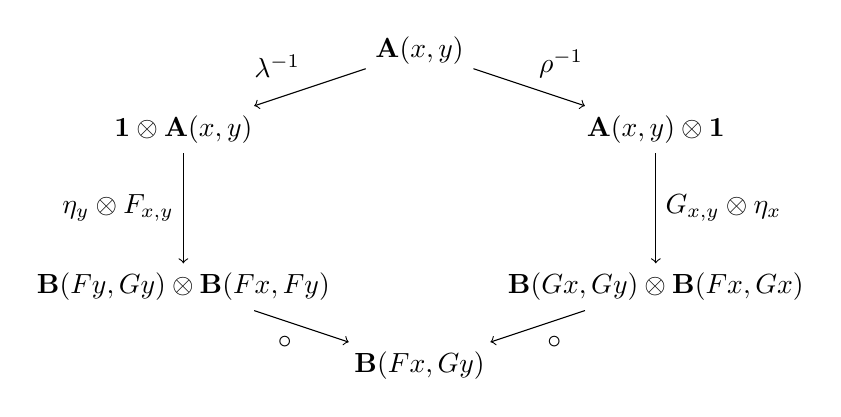
\begin{tikzpicture}
            \node (A) at (0, 0) {$\mathbf{A}(x,y)$};
            \node (IA) at (-3, -1) {$\mathbf{1}\otimes\mathbf{A}(x,y)$};
            \node (AI) at (3, -1) {$\mathbf{A}(x,y)\otimes\mathbf{1}$};
            \node (BF) at (-3, -3) {$\mathbf{B}(Fy,Gy)\otimes\mathbf{B}(Fx,Fy)$};
            \node (BG) at (3, -3) {$\mathbf{B}(Gx,Gy)\otimes\mathbf{B}(Fx,Gx)$};
            \node (B) at (0, -4) {$\mathbf{B}(Fx,Gy)$};
            \draw[->] (A) -- node[above left]{$\lambda^{-1}$} (IA);
            \draw[->] (A) -- node[above right]{$\rho^{-1}$} (AI);
            \draw[->] (IA) -- node[left]{$\eta_y\otimes F_{x,y}$} (BF);
            \draw[->] (AI) -- node[right]{$G_{x,y}\otimes\eta_x$} (BG);
            \draw[->] (BF) -- node[below left]{$\circ$} (B);
            \draw[->] (BG) -- node[below right]{$\circ$} (B);
        \end{tikzpicture}
        \caption{$\mathcal{V}$-naturality diagram.}
        \label{fig:v_naturality}
     \end{figure}

\subsection{Enriched constructions}

    \newdef{Functor tensor product}{\index{tensor product!of functors}\label{cat:functor_tensor_product}
        Consider a covariant functor $\func{G}{C}{\mathcal{V}}$ and a contravariant functor $\cfunc{F}{C}{\mathcal{V}}$ into a monoidal category $\mathcal{V}$, where $\mathbf{C}$ does not have to be enriched over $\mathcal{V}$. The tensor product of $F$ and $G$ is defined as the following coend:
        \begin{gather}
            F\otimes_{\mathbf{C}}G := \int^{x\in\mathbf{C}}Fx\otimes Gx\,.
        \end{gather}
    }
    It should be noted that the above tensor product does not produce a new functor, instead it only gives an object in $\mathcal{V}$. A different type of tensor product, one that does give a functor, exists in the enriched setting (note that there is no relation between these two definitions).
    \newdef{Day convolution}{\index{Day convolution}
        Consider a monoidally cocomplete category $\mathcal{V}$, i.e.~cocomplete monoidal category for which the tensor product bifunctor is cocontinuous in each argument, together with a $\mathcal{V}$-enriched category $\mathbf{C}$. The convolution or tensor product (if it exists) of two $\mathcal{V}$-enriched functors $\func{F,G}{C}{\mathcal{V}}$ is defined as the following coend:
        \begin{gather}
            F\otimes_{\mathrm{Day}}G := \iint^{x,y\in\mathbf{C}}\mathbf{C}(x\otimes y,-)\otimes Fx\otimes Gy\,.
        \end{gather}
    }
    \begin{property}[Monoidal structure]
        When $\mathbf{M}$ is closed symmetric monoidal, Day convolution is associative and, hence, defines a monoidal structure on the functor category $\funccat{C}{M}$. The tensor unit is given by the functor (co)represented by the tensor unit in $\mathbf{C}$.
    \end{property}

    \newdef{Copower}{\index{co-!power}\index{power}\label{hda:power} % Both terms are indexed since copowers are rather important on their own.
        Consider a $\mathcal{V}$-enriched category $\mathbf{C}$. The copower (or \textbf{tensor}) functor $\func{\cdot}{\mathcal{V}\times C}{C}$ is defined by the following natural isomorphism:
        \begin{gather}
            \mathbf{C}(v\cdot x,y)\cong\mathcal{V}\bigl(v,\mathbf{C}(x,y)\bigr)\,.
        \end{gather}
        Dually, the \textbf{power} (or \textbf{cotensor}) functor $\func{[-,-]}{\mathcal{V}\times C}{C}$ is defined by the following natural isomorphism:
        \begin{gather}
            \mathbf{C}\bigl(x,[v,y]\bigr)\cong\mathcal{V}\bigl(v,\mathbf{C}(x,y)\bigr)\,.
        \end{gather}
        If an enriched category admits all (co)powers, it is said to be \textbf{(co)powered} (over its enriching category).
    }
    \remark{\Cref{cat:internal_symmetry} says that every (closed) symmetric monoidal category $\mathbf{M}$ is powered over itself, the power just being the internal hom. The same holds for the copower, which is just the usual tensor product functor.}

    \begin{example}[Disjoint unions]
        Every (co)complete (locally) small category $\mathbf{C}$ admits the structure of a $\mathbf{Set}$-(co)powered category:
        \begin{gather}
            \begin{aligned}
                x^S &:= \prod_{s\in S}x\,,\\
                S\cdot x &:= \bigsqcup_{s\in S}x\,.
            \end{aligned}
        \end{gather}
    \end{example}

    The definition and properties of internal hom-functors and (co)powers can be formalized as follows.
    \newdef{Two-variable adjunction}{\index{adjunction}\label{cat:two_variable_adjunction}
        Consider three categories $\mathbf{A,B}$ and $\mathbf{C}$. A two-variable adjunction $\mathbf{A}\times\mathbf{B}\rightarrow\mathbf{C}$ consists of three bifunctors:
        \begin{itemize}
            \item $\func{-\otimes-}{A\times B}{C}$,
            \item $\hom_L:\mathbf{A}^{\text{op}}\times\mathbf{C}\rightarrow\mathbf{B}$, and
            \item $\hom_R:\mathbf{B}^{\text{op}}\times\mathbf{C}\rightarrow\mathbf{A}$
        \end{itemize}
        admitting the following natural isomorphisms:
        \begin{gather}
            \mathbf{C}(x\otimes y,z)\cong\mathbf{A}\bigl(x,\hom_R(y,z)\bigr)\cong\mathbf{B}\bigl(y,\hom_L(x,z)\bigr)\,.
        \end{gather}
        It should be noted that fixing any of the variables gives rise to ordinary adjunctions in the sense of \cref{section:adjunction}.
    }
    \begin{property}[Powers and copowers]
        A category $\mathbf{C}$ enriched over a monoidal category $\mathcal{V}$ is powered and copowered over $\mathcal{V}$ exactly if the hom-functor $\mathbf{C}^{\text{op}}\times\mathbf{C}\rightarrow\mathcal{V}$ is the right adjoint in an enriched two-variable adjunction. The power and copower functors are then given by the other two adjoints.
    \end{property}

    The co-Yoneda lemma~\ref{cat:ninja_yoneda} can be generalized to the enriched setting.
    \begin{property}[Ninja Yoneda lemma]\index{Yoneda!reduction}\index{co-!Yoneda|see{Yoneda, reduction}}\label{cat:enriched_ninja_yoneda}
        Let $\cfunc{F}{C}{\mathcal{V}}$ be a contravariant functor (similar statements hold for covariant functors).
        \begin{gather}
            \begin{aligned}
                \int^{x\in\mathbf{C}}\mathbf{C}(-,x)\otimes Fx &\cong F\\
                \int_{x\in\mathbf{C}}\mathcal{V}\bigl(\mathbf{C}(x,-),Fx\bigr) &\cong F\,.
            \end{aligned}
        \end{gather}
    \end{property}

    The following definition constructs Kan extensions in the enriched setting (these can be shown to reduce to \cref{cat:kan_extension} when enriching over $\mathbf{Set}$).
    \newadef{Kan extension}{\index{Kan!extension}\label{cat:enriched_kan_extension}
        Let $\mathbf{A,B}$ and $\mathbf{C}$ be categories enriched over a monoidal category $\mathcal{V}$. If $\mathbf{B}$ is assumed to be copowered over $\mathcal{V}$, left Kan extension of $\func{F}{A}{B}$ along $\func{G}{A}{C}$ can be defined through a coend:
        \begin{gather}
            \mathrm{Lan}_GF := \int^{x\in\mathbf{A}}\mathbf{C}(Gx,-)\cdot Fx\,.
        \end{gather}
        If $\mathbf{B}$ is assumed to be powered over $\mathcal{V}$, right Kan extension can be defined through an end:
        \begin{gather}
            \mathrm{Ran}_GF := \int_{x\in\mathbf{A}}\bigl[\mathbf{C}(-,Gx),Fx\bigr]\,.
        \end{gather}
        If $F$ is contravariant, the arguments of the hom-functors should simply be interchanged.
    }
    \remark{By choosing $\mathcal{V}=\mathbf{Set},\mathbf{C}=\mathbf{A}$ and $G=\mathbbm{1}_{\mathbf{A}}$ in the previous definition, one obtains the ninja Yoneda lemma~\ref{cat:ninja_yoneda}.}
    \begin{property}
        As already remarked in \cref{cat:preservation_kan_extension}, Kan extensions computed using (co)ends as above are strong.
    \end{property}

    \newadef{Functor tensor product}{\index{tensor product!of functors}\label{cat:copower_product}
        Let $\mathbf{B}$ be a $\mathcal{V}$-enriched category. Consider a covariant functor $\func{G}{A}{B}$ and a contravariant functor $\cfunc{F}{A}{\mathcal{V}}$. The tensor product (\cref{cat:functor_tensor_product}) can be generalized whenever $\mathbf{B}$ is copowered over $\mathcal{V}$:
        \begin{gather}
            F\otimes_{\mathbf{A}}G := \int^{x\in\mathbf{A}}Fx\cdot Gx\,.
        \end{gather}
    }

\subsection{Weighted (co)limits}\index{limit!weighted}\label{section:weighted_limits}

    In this section, the definition of ordinary limits and, in particular, the defining universal property~\ref{cat:limit_uproperty} is revisited. In this construction, the constant functor $\Delta_x$ was one of the main ingredients. This functor can be factorized as $\mathbf{I}\rightarrow1\rightarrow\mathbf{C}$, where $1$ denotes the terminal category. At the level of morphisms, this factorization takes the form $\mathbf{I}(i,j)\rightarrow\ast\rightarrow\mathbf{C}(x,x)$, where $\ast$ denotes the terminal one-element set. However, whenever the enriching context is not $\mathbf{Set}$, one does not necessarily have access to a terminal object.

    To avoid this issue, limits will first be redefined as representing objects. To this end, consider a general diagram $\func{D}{I}{C}$. By postcomposition with the Yoneda embedding, one obtains the presheaf-valued diagram $\mathbf{C}(-,D-):\mathbf{I}\rightarrow[\mathbf{C}^{\text{op}},\mathbf{Set}]$. Since presheaf categories are complete (\cref{cat:complete_presheaf_category}), the limit of this diagram exists:
    \begin{gather}
        \mathbf{Set}\bigl(S,\lim\mathbf{C}(x,D-)\bigr)\cong\funccat{I}{Set}\bigl(\Delta_S,\mathbf{C}(x,D-)\bigr)\,.
    \end{gather}
    By restricting to the terminal set $S=\ast$, one obtains
    \begin{gather}
        \lim\mathbf{C}(x,D-)\cong\funccat{I}{Set}\bigl(\Delta_\ast,\mathbf{C}(x,D-)\bigr)\,.
    \end{gather}
    If this presheaf is representable, one can use the continuity of the hom-functor, together with the fact that the Yoneda embedding is fully faithful, to show that the representing object is (isomorphic to) $\lim D$, i.e.
    \begin{gather}
        \funccat{I}{Set}\bigl(\Delta_\ast,\mathbf{C}(x,D-)\bigr)\cong\mathbf{C}(x,\lim D)\,.
    \end{gather}

    \todo{CLEAN THIS UP (note that continuity and pointwise definition was already mentioned for ordinary limits)}

    \newdef{Weighted limit}{\index{limit!conical}\label{cat:weighted_limit}
        The above construction can now be generalized by replacing the constant functor $\Delta_\ast$ by any functor $\func{W}{I}{Set}$. A representing object is then called the $W$-weighted limit of $D$. This object is often denoted by $\wlim{W}D$ or $\{W,D\}$. To distinguish weighted limits from ordinary ones, the latter are sometimes called \textbf{conical limits}.
    }

    \begin{remark}
        A motivation for this construction is the following. As was already pointed out in \cref{cat:global_elements_remark}, the mere knowledge of global elements $1\rightarrow x$ is often not enough to characterize an object $x$. In general, one should look at the collection of generalized elements. When applying this ideology to the case of cones, one sees that replacing the functor $\Delta_\ast$ by a more general functor is the same as replacing the global elements $\ast\rightarrow Di$ by generalized elements $Wi\rightarrow Di$.
    \end{remark}

    The generalization to the enriched setting is now evident. There is no reference to the terminal object left, so one can replace $\mathbf{Set}$ by any enriching category. In the enriched setting, (co)end formulas for (weighted) limits will often be used.
    \newformula{Enriched weighted limits}{\label{cat:weighted_limits}
        By expressing the natural transformations as an end as in \cref{cat:natural_end} and by using the canonical powering in $\mathbf{Set}$, one can express ordinary weighted limits as follows:
        \begin{gather}
            \wlim{W}D\cong\int_{i\in\mathbf{I}}[Wi,Di]\,.
        \end{gather}
        The generalization to other enriching categories is now straightforward. Consider a diagram $\func{D}{I}{C}$ and a weight functor $\func{W}{I}{\mathcal{V}}$, where $\mathbf{C}$ is $\mathcal{V}$-enriched. If $\mathbf{C}$ is powered over $\mathcal{V}$, the $W$-weighted limit of $D$ is defined by the same formula as above:
        \begin{gather}
            \wlim{W}D:=\int_{i\in\mathbf{I}}[Wi,Di]\,.
        \end{gather}
        In a similar way, one can define weighted colimits in copowered $\mathcal{V}$-categories as coends:
        \begin{gather}
            \colim^WD:=\int^{i\in\mathbf{I}}Wi\cdot Di\,.
        \end{gather}
        Here, the weight functor $W$ is required to be contravariant since colimits (and cocones in general) are natural transformations between contravariant functors.
    }
    \begin{property}[Weighted limits are Homs]
        In the case $\mathbf{C}=\mathcal{V}$, the powering becomes the internal hom and, therefore, one sees that weighted limits are given by (enriched) natural transformations (as was the case for ordinary conical limits).
    \end{property}

    In the following example, the weighted colimit is calculated with respect to the Yoneda embedding.
    \begin{example}[Hom-functor]
        Consider a diagram $\func{D}{I}{C}$. When using the Yoneda embedding $\mathcal{Y}i = \mathbf{I}(-,i)$ as the weight functor, one obtains the following property by virtue of the Yoneda lemma:
        \begin{gather}
            \label{cat:weighted_hom_colimit}
            \colim^{\mathcal{Y}i}D\cong Di\,.
        \end{gather}
        A similar statement for weighted limits can be obtained with the covariant Yoneda embedding.
    \end{example}
    \newadef{Weighted (co)limits}{\index{limit!weighted}
        The above property can be used to axiomatize small weighted (co)limits in bicomplete categories:
        \begin{enumerate}
            \item\textbf{Yoneda}: For every object $i\in\ob{I}$, there exist isomorphisms
            \begin{gather}
                \wlim{\mathbf{I}(i,-)}D\cong Di\qquad\text{and}\qquad\colim^{\mathbf{I}(-,i)}D\cong Di\,.
            \end{gather}
            \item\textbf{Cocontinuity}: The weighted (co)limit functors are cocontinuous in the weights.
        \end{enumerate}
    }

    One can also express Kan extensions as weighted limits (this simply follows from \cref{cat:enriched_kan_extension}).
    \begin{property}[Kan extensions]\index{Kan!extension}
        Consider functors $\func{F}{A}{B}$ and $\func{G}{A}{C}$. If, for every $x\in\ob{C}$, the weighted limit $\wlim{\mathbf{C}(x,G-)}F$ exists, these limits can be combined into a functor that can be shown to be the right Kan extension $\mathrm{Ran}_GF$. The left Kan extension can be obtained as a weighted colimit.
    \end{property}

    \begin{property}[Category of elements]\index{category!of elements}
        The weighted (co)limits of a functor (over $\mathbf{Set}$) can also be expressed in terms of the category of elements (\cref{cat:category_of_elements}) of the weight:
        \begin{gather}
            \wlim{W}F\cong\lim F\circ\mathbf{C}_W\,,
        \end{gather}
        where the limit on the right-hand side is a conical limit.

        The reason for the (co)end notation for categories of elements can also be explained by noting that these can actually be obtained as weighted (co)limits or (co)ends (here given for covariants functors):
        \begin{gather}
            \mathrm{El}(F) \cong \int^{c\in\mathbf{C}}Jc\times\mathrm{Disc}\,Fc\,,
        \end{gather}
        where $\cfunc{J}{C}{Cat}:c\mapsto c/\mathbf{C}$ assigns undercategories and $\func{\mathrm{Disc}}{Set}{Cat}$ sends sets to discrete categories.
    \end{property}

\section{Abelian categories}\label{section:abelian_categories}
\subsection{Additive categories}

    \newdef{Pre-additive category}{
        A (locally small) category enriched over $\mathbf{Ab}$, i.e.~a category in which every hom-set is an Abelian group and composition is bilinear.
    }

    \begin{property}\index{zero!object}
        Let $\mathbf{A}$ be a pre-additive category. The following statements are equivalent for an object $x\in\ob{A}$:
        \begin{itemize}
            \item $x$ is initial,
            \item $x$ is final, or
            \item $\mathbbm{1}_x = 0$.
        \end{itemize}
        It follows that every initial/terminal object in a pre-additive category is automatically a zero object (\cref{cat:zero_object}).
    \end{property}
    \begin{property}[Biproducts]\index{bi-!product}\index{direct!sum}
        In a pre-additive category, the following isomorphism holds for all finitely indexed sets $\{x_i\}_{i\leq n}$:
        \begin{gather}
            \prod_{i\leq n}x_i\cong\bigsqcup_{i\leq n}x_i\,.
        \end{gather}
        Finite (co)products in pre-additive categories are often called \textbf{direct sums}. In general, if a product and coproduct exist and are isomorphic, one also speaks of a \textbf{biproduct}.
    \end{property}

    \newdef{Additive category}{\index{additive!category}
        A pre-additive category admitting all finite products (and, hence, biproducts).
    }

    When working with additive categories, it is generally assumed that the associated functors are of a specific type.
    \newdef{Additive functor}{\index{additive!functor}\label{cat:additive_functor}
        Let $\mathbf{A},\mathbf{A'}$ be additive categories. A functor $\func{F}{A}{A'}$ is said to be additive if it preserves finite biproducts:
        \begin{enumerate}
            \item It preserves zero objects: $F\,0_{\mathbf{A}}\cong0_{\mathbf{A}'}$.
            \item There exists a natural isomorphism $F(x\oplus y)\cong Fx\oplus Fy$.
        \end{enumerate}
        This notion can be generalized to pre-additive categories. A functor between pre-additive categories is said to be additive if it acts by group morphisms on hom-spaces.
    }

    \newdef{Grothendieck group}{\index{Grothendieck!group}
        Let $\mathbf{A}$ be an additive category and consider its decategorification (\cref{cat:decategorification}). This set carries the structure of an Abelian monoid and, hence, the Grothendieck construction (\cref{group:grothendieck_completion}) can be applied to obtain an Abelian group $K(\mathbf{A})$. This group is called the Grothendieck group of $\mathbf{A}$.
    }

    In a (pre-)additive category, one can define some classical notions from (homological) algebra such as images and kernels.
    \newdef{Kernel}{\index{kernel}
        Let $f:x\rightarrow y$ be a morphism. A\footnote{`\textit{A}' since the kernel of a morphism is only determined up to an isomorphism.} kernel of $f$ is a morphism $k:z\rightarrow x$ such that:
        \begin{gather}
            f\circ k = 0
        \end{gather}
        and such that it is universal with respect to this property. This implies that a kernel of $f$ could equivalently be defined as the equalizer of $f$ and $0$.
    }
    \begin{notation}[Kernel]
        If the kernel of $f:x\rightarrow y$ exists, it is denoted by $\ker(f)$.
    \end{notation}

    \newdef{Cokernel}{
        Let $f:x\rightarrow y$ be a morphism. A cokernel of $f$ is a morphism $p:y\rightarrow z$ such that:
        \begin{gather}
            p\circ f = 0
        \end{gather}
        and such that it is universal with respect to this property. This implies that a cokernel of $f$ could equivalently be defined as the coequalizer of $f$ and 0.
    }
    \begin{notation}[Cokernel]
        If the cokernel of $f:x\rightarrow y$ exists, it is denoted by $\mathrm{coker}(f)$.
    \end{notation}

    \begin{remark}
        The name and notation of the kernel and the cokernel (in the categorical sense) are explained by remarking that $\ker(f)$ represents the functor
        \begin{gather}
            F:z\mapsto\ker\bigl(\mathbf{C}(z,x)\rightarrow\mathbf{C}(z,y)\bigr)\,,
        \end{gather}
        where $\ker$ denotes the algebraic kernel (\cref{group:kernel}), and similarly for the cokernel.
    \end{remark}

    \newdef{Pseudo-Abelian category}{\label{cat:pseudo_abelian}
        An additive category in which every projection/idempotent has a kernel.
    }
    \newdef{Pre-Abelian category}{
        An additive category in which every morphism has a kernel and cokernel.
    }
    \newdef{Abelian category}{\index{Abelian!category}
        A pre-Abelian category in which every mono is a kernel and every epi is a cokernel or, equivalently, if for every morphism $f$ there exists an isomorphism
        \begin{gather}
            \coker\bigl(\ker(f)\bigr)\cong\ker\bigl(\coker(f)\bigr)\,.
        \end{gather}
    }

    \begin{property}
        Every Abelian category is balanced (\cref{cat:balanced}).
    \end{property}

    \begin{property}[Injectivity and surjectivity]
        In Abelian categories, a morphism is monic if and only if it is injective, i.e.~its kernel is 0. Analogously, a morphism is epic if and only if it is surjective, i.e.~its cokernel is 0.
    \end{property}

    \newdef{Linear category}{\index{category!linear}
        Let $\mathbf{Vect}_k$ denote the category of vector spaces over the base field $k$. A $k$-linear category is a category enriched over $\mathbf{Vect}_k$. (If the base field is clear, it is often left implicit.)
    }

\subsection{Exact functors}

    In the setting of additive categories, \cref{cat:exact_functor} can be characterized more simply.
    \newdef{Exact functor}{\index{exact!functor}
        Let $\func{F}{A}{A'}$ be an additive functor between additive categories.
        \begin{itemize}
            \item $F$ is left exact if it preserves kernels.
            \item $F$ is right exact if it preserves cokernels.
            \item $F$ is exact if it is both left and right exact.
        \end{itemize}
    }
    \begin{result}
        The previous definition implies the following properties (which can, in fact, be used as an alternative definition):
        \begin{itemize}
            \item If $F$ is left exact, it maps an exact sequence of the form \[0\longrightarrow x\longrightarrow y\longrightarrow z\]
            to an exact sequence of the form \[0\longrightarrow Fx\longrightarrow Fy\longrightarrow Fz\,.\]
            \item If $F$ is right exact, it maps an exact sequence of the form \[x\longrightarrow y\longrightarrow z\longrightarrow 0\]
            to an exact sequence of the form \[Fx\longrightarrow Fy\longrightarrow Fz\longrightarrow 0\,.\]
            \item If $F$ is exact, it maps short exact sequences to short exact sequences.
        \end{itemize}
    \end{result}

    \begin{notation}[Left or right]
        The category of left modules ${}_R\mathbf{Mod}$ over a ring $R$ is equivalent (as an Abelian category) to the category of right modules $\mathbf{Mod}_{\op{R}}$ over the opposite ring $R$. For this reason, one often makes no difference between left and right modules (only bimodules are truly relevant) and `the category of $R$-modules' is just denoted by $R\mathbf{Mod}$.
    \end{notation}

    \begin{theorem}[Freyd--Mitchell embedding theorem]\index{Freyd--Mitchell embedding theorem}\index{embedding!theorem|see{Freyd--Mitchell}}\label{cat:freyd_mitchell}
        Every small Abelian category admits a fully faithful, exact functor into a category of the form $R\mathbf{Mod}$ for some unital ring $R$.
    \end{theorem}

    \begin{theorem}[Eilenberg--Watts]\index{Eilenberg--Watts}
        Let $R,S$ be two (not necessarily unital) rings. The tensor product functor induces an equivalence between the category of $R\text{-}S$-bimodules and the category of cocontinuous functors $R\mathbf{Mod}\rightarrow S\mathbf{Mod}$.
    \end{theorem}

\subsection{Finiteness}

    \newdef{Simple object}{\index{simple!object}
        Let $\mathbf{A}$ be an Abelian category. An object $a\in\ob{A}$ is said to be simple if the only subobjects of $a$ are $0$ and $a$ itself. An object is said to be semisimple if it is a direct sum of simple obejcts.
    }
    \newdef{Semisimple category}{
        A category is said to be semisimple if every object is semisimple, where, in general, the direct sums are taken over finite index sets.
    }

    \newdef{Jordan--H\"older series}{\index{finite}\index{Jordan--H\"older!series}
        A filtration (\cref{set:filtration})
        \begin{gather}
            0\longrightarrow x_1\longrightarrow x_2\longrightarrow\cdots\longrightarrow x_n=x
        \end{gather}
        of an object $x$ is said to be a Jordan--H\"older series if the quotient objects $x_i/x_{i-1}$ are simple for all $i\leq n$. If the series has finite length, the object $x$ is said to be \textbf{finite}.
    }
    \begin{theorem}[Jordan--H\"older]\index{Jordan--H\"older}
        If an object in an Abelian category is finite, all of its Jordan--H\"older series have the same length. In particular, the multiplicities of simple objects are the same for all such series.
    \end{theorem}

    \begin{theorem}[Krull--Schmidt]\index{Krull--Schmidt}\index{indecomposable}
        Any object in an Abelian category of finite length admits a unique decomposition as a direct sum of indecomposable objects\footnote{An object is \textbf{indecomposable} if it cannot be written as a direct sum of its subobjects.}.
    \end{theorem}

    \newdef{Locally finite}{\label{cat:locally_finite}
        A $\mathfrak{K}$-linear Abelian category is said to be locally finite if it satisfies the following conditions:
        \begin{enumerate}
            \item every hom-space is finite-dimensional, and
            \item every object has finite length.
        \end{enumerate}
    }
    \newdef{Finite}{\index{finite}\index{projective!cover}
        A $\mathfrak{K}$-linear Abelian category is said to be finite if it satisfies the following conditions:
        \begin{enumerate}
            \item it is locally finite,
            \item it has enough projectives or, equivalently, every simple object has a \textit{projective cover}, and
            \item the set of isomorphism classes of simple objects is finite.
        \end{enumerate}
    }

    \begin{theorem}[Schur's lemma]\index{Schur!lemma}\label{cat:schur_lemma}
        Let $\mathbf{A}$ be an Abelian category. For every two simple objects $x,y\in\ob{A}$, all nonzero morphisms $x\rightarrow y$ are isomorphisms. In particular, if $x,y$ are two non-isomorphic simple objects, then $\mathbf{A}(x,y)=0$. Furthermore, $\mathbf{A}(x,x)$ is a division ring for every simple object $x\in\ob{A}$.
    \end{theorem}
    \begin{result}
        If $\mathbf{A}$ is locally finite and $\mathfrak{K}$ is algebraically closed, then $\mathbf{A}(x,x)\cong\mathfrak{K}$ for all simple objects $x\in\ob{A}$. This follows from the fact that the only finite-dimensional division algebra over an algebraically closed field is the field itself.
    \end{result}

    The Freyd--Mitchell theorem~\ref{cat:freyd_mitchell} can be adapted to the finite linear case as follows.
    \begin{theorem}[Deligne]\index{Deligne}
        Every finite $\mathfrak{K}$-linear Abelian category is $\mathfrak{K}$-linearly equivalent to a category of the form $A\mathbf{Mod}^{\emph{fin}}$ for $A$ a finite-dimensional $\mathfrak{K}$-algebra.
    \end{theorem}

    \begin{construct}[Deligne tensor product]\index{Deligne|seealso{tensor product}}\index{tensor product!Deligne}
        Let $\mathbf{A},\mathbf{B}$ be two Abelian categories. Their Deligne (tensor) product is defined (if it exists) as the category $\mathbf{A}\boxtimes\mathbf{B}$ for which there exists a bijection between right exact functors $\mathbf{A}\boxtimes\mathbf{B}\rightarrow\mathbf{C}$ and right exact functors $\mathbf{A}\times\mathbf{B}\rightarrow\mathbf{C}$ (the latter being right exact in each argument).

        For finite Abelian categories, it can be shown that their Deligne product always exists. By the Deligne embedding theorem, one can find an explicit description. Consider two finite-dimensional $\mathfrak{K}$-algebras $A,B$. The category $A\mathbf{Mod}^{\text{fin}}\boxtimes B\mathbf{Mod}^{\text{fin}}$ is equivalent to the category $(A\otimes_{\mathfrak{K}}B)\mathbf{Mod}^{\text{fin}}$.
    \end{construct}

\section{Duality}\label{section:duality}

    \newdef{Dual object}{\index{dual!object}\index{evaluation}\index{unit}\label{hda:dual}
        Let $(\mathbf{C},\otimes,\mathbf{1})$ be a monoidal category and consider an object $x\in\ob{C}$. A left dual\footnote{$x$ is called the \textbf{right dual} of $x^*$. The right dual of $y$ is often denoted by ${}^*y$.} of $x$ is an object $x^*\in\ob{C}$ together with two morphisms $\eta:\mathbf{1}\rightarrow x\otimes x^*$ and $\varepsilon:x^*\otimes x\rightarrow\mathbf{1}$, called the \textbf{unit} and \textbf{counit} morphisms\footnote{Also called the \textbf{coevaluation} and \textbf{evaluation} morphisms.}, such that the diagrams in \cref{fig:dual_objects} commute. $x$ is said to be \textbf{dualizable} if it admits a left dual.
    }

    \begin{figure}[ht!]
        \centering
        \begin{subfigure}[b]{0.49\textwidth}
            \centering
            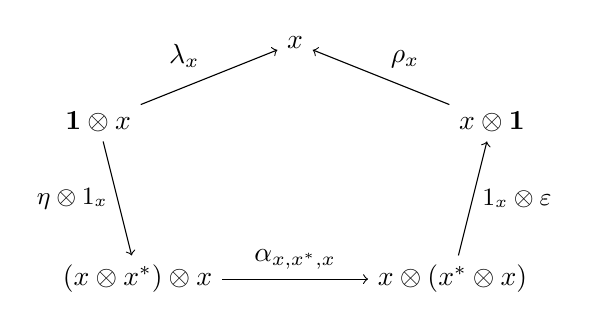
\begin{tikzpicture}
                \node (X) at (0, 0) {$x$};
                \node (1X) at (-2.5, -1) {$\mathbf{1}\otimes x$};
                \node (X1) at (2.5, -1) {$x\otimes\mathbf{1}$};
                \node (1XXX) at (-2, -3) {$(x\otimes x^*)\otimes x$};
                \node (XXX1) at (2, -3) {$x\otimes(x^*\otimes x)$};
                \draw[->] (1X) -- node[above left]{$\lambda_x$} (X);
                \draw[->] (X1) -- node[above right]{$\rho_x$} (X);
                \draw[->] (1X) -- node[left]{\small $\eta\otimes\mathbbm{1}_x$} (1XXX);
                \draw[->] (XXX1) -- node[right]{\small $\mathbbm{1}_x\otimes\varepsilon$} (X1);
                \draw[->] (1XXX) -- node[above]{$\alpha_{x,x^*,x}$} (XXX1);
            \end{tikzpicture}
            \caption{Dual object I.}
            \label{fig:dual_object1}
        \end{subfigure}
        \begin{subfigure}[b]{0.49\textwidth}
            \centering
            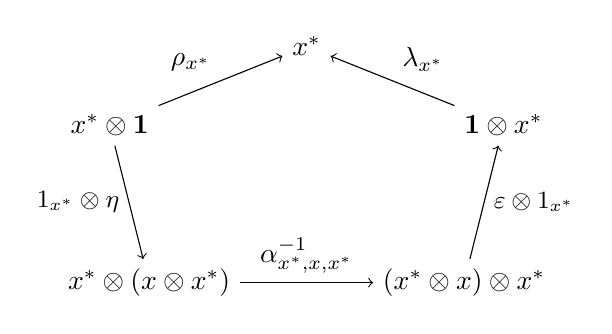
\begin{tikzpicture}
                \node (X) at (0, 0) {$x^*$};
                \node (X1) at (-2.5, -1) {$x^*\otimes\mathbf{1}$};
                \node (1X) at (2.5, -1) {$\mathbf{1}\otimes x^*$};
                \node (XXX1) at (-2, -3) {$x^*\otimes(x\otimes x^*)$};
                \node (1XXX) at (2, -3) {$(x^*\otimes x)\otimes x^*$};
                \draw[->] (X1) -- node[above left]{$\rho_{x^*}$} (X);
                \draw[->] (1X) -- node[above right]{$\lambda_{x^*}$} (X);
                \draw[->] (X1) -- node[left]{\small $\mathbbm{1}_{x^*}\otimes\eta$} (XXX1);
                \draw[->] (1XXX) -- node[right]{\small $\varepsilon\otimes\mathbbm{1}_{x^*}$} (1X);
                \draw[->] (XXX1) -- node[above]{$\alpha^{-1}_{x^*,x,x^*}$} (1XXX);
            \end{tikzpicture}
            \caption{Dual object II.}
            \label{fig:dual_object2}
        \end{subfigure}
        \caption{Dualizable objects.}
        \label{fig:dual_objects}
    \end{figure}

    \newdef{Rigid category}{\index{category!rigid}\index{category!autonomous}
        A monoidal category that has all duals. These categories are also said to be \textbf{autonomous}. If only left (resp.~right) duals exist, the category is said to be left (resp.~right) rigid.
    }

    \begin{property}[Braided categories]\label{hda:braided_rigid}
        In general, it is not true that left and right duals coincide. However, in a braided monoidal category this is the case.
    \end{property}

    \newdef{Compact closed category}{\index{category!compact closed}
        A symmetric rigid category.
    }

    \begin{example}[FinVect]\index{dual!space}\index{resolution!of the identity}
        Consider the category $\mathbf{FinVect}$ of finite-dimensional vector spaces (the ground field is assumed to be $\mathbb{R}$). The categorical dual of a vector space $V$ is the algebraic dual $V^*$. The unit morphism is given by the `resolution of the identity':
        \begin{gather}
            \eta:\mathbf{1}\rightarrow V\otimes V^*:1\mapsto\sum_{i=1}^{\dim(V)}e_i\otimes\phi^i\,,
        \end{gather}
        where $\{e_i\}$ and $\{\phi^i\}$ are dual bases of $V$ and $V^*$, respectively.

        It should be noted that the category $\mathbf{Vect}$ of all vector spaces is not rigid. By \cref{hda:braided_rigid} above, left and right duals coincide in any braided monoidal category (such as $\mathbf{Vect}$), but for infinite-dimensional vector spaces it is known that $A\cong(A^*)^*$ never holds and, as such, rigidity cannot be extended to $\mathbf{Vect}$.
    \end{example}

    \begin{property}[Tannaka duality]\index{Tannaka duality}
        Consider the category $\mathcal{V}=\mathbf{FinVect}_k$. Using coends, one can reconstruct the base field from its modules, i.e.~the objects in $\mathcal{V}$:
        \begin{gather}
            \int^{V\in\mathcal{V}}V^*\otimes V\cong k\,.
        \end{gather}
        This result can be shown to hold for all compact closed categories $\mathcal{V}$. In this context, it is known as \textbf{Tannaka reconstruction}. A more general statement goes as follows:
        \begin{gather}
            \int^{V\in\mathcal{V}}\mathcal{V}(V,-)\otimes V\cong\mathrm{id}_{\mathcal{V}}\,.
        \end{gather}
        For $\mathcal{V}=\mathbf{FinVect}_k$, the components $\eta_V:\mathcal{V}(V,V)\rightarrow k$ of the coend can be shown to coincide with the trace and, as such, the trace obtains a universal property.
    \end{property}
    \begin{remark}
        This property can also be generalized by replacing $\mathcal{V}$ by a category of modules $A\mathbf{Mod}$ for some finite-dimensional algebra $A$. The end and coend give the algebra $A$ and its dual $A^*$, respectively.
    \end{remark}

    For certain purposes, it is useful to slightly weaken the notion of compact closed categories (e.g.~\citet{kissinger_categorical_2019,barr_-autonomous_1991}).
    \newdef{$\ast$-autonomous category}{\index{category!autonomous}\label{hda:star_autonomous_category}
        A symmetric monoidal category $(\mathbf{C},\otimes,\mathbf{1})$ with a fully faithful dualization functor $\cfunc{\ast}{C}{C}$ such that
        \begin{gather}
            \mathbf{C}(x\otimes y,z^*)\cong\mathbf{C}\bigl(x,(y\otimes z)^*\bigr)
        \end{gather}
        for all $x,y,z\in\ob{C}$.
    }
    \begin{property}[de Morgan duality]\index{de Morgan!duality}\label{hda:de_morgan_duality}
        If $(\mathbf{C},\otimes,\mathbf{1},\ast)$ is a $\ast$-autonomous category, it admits a second $\ast$-autonomous structure $(\mathbf{C},\dualampersand,\bot,\ast)$ given by
        \begin{gather}
            x\dualampersand y := (x^*\otimes y^*)^*
        \end{gather}
        for all $x,y\in\ob{C}$ and
        \begin{gather}
            \bot := \mathbf{1}^*\,.
        \end{gather}
    \end{property}

    \begin{property}[Involution]
        Note that the definition of $\ast$-autonomous categories implies that
        \begin{gather}
            x\cong x^{**}
        \end{gather}
        for all $x\in\ob{C}$. Moreover, $\ast$-autonomous categories are closed with the internal hom given by:
        \begin{gather}
            [x,y] = x^*\dualampersand y \cong (x\otimes y^*)^*\,.
        \end{gather}
        A $\ast$-autonomous category is compact closed if and only if duality is compatible with tensor products:
        \begin{gather}
            (x\otimes y)^*\cong x^*\otimes y^*\,.
        \end{gather}
        Equivalently, a $\ast$-autonomous category is compact closed if and only if the de Morgan-dual monoidal structures coincide.
    \end{property}

    \newdef{Symmetric monoidal dagger category}{\index{category!dagger}
        A symmetric monoidal category $(\mathbf{C},\otimes,\mathbf{1})$ that also carries the structure of a dagger category (\cref{cat:dagger_category}) such that
        \begin{gather}
            (f\otimes g)^\dag = f^\dag\otimes g^\dag
        \end{gather}
        and such that the coherence and braiding morphisms are unitary.
    }
    \newdef{Dagger-compact category}{
        A symmetric monoidal dagger category that is also a compact closed category such that the following diagram commutes for all objects:
        \begin{gather*}
            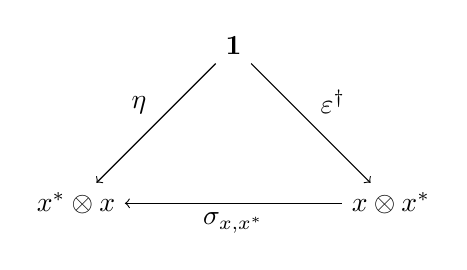
\begin{tikzpicture}
                \node (1) at (0, 0) {$\mathbf{1}$};
                \node (X*X) at (-2, -2) {$x^*\otimes x$};
                \node (XX*) at (2, -2) {$x\otimes x^*$};
                \draw[->] (1) -- node[above left]{$\eta$} (X*X);
                \draw[->] (1) -- node[above right]{$\varepsilon^\dagger$} (XX*);
                \draw[<-] (X*X) -- node[below]{$\sigma_{x,x^*}$} (XX*);
            \end{tikzpicture}
        \end{gather*}
    }

    The trace on $\mathbf{FinVect}$ can be generalized as follows.
    \newdef{Trace}{\index{trace}
        Let $(\mathbf{C},\otimes,\mathbf{1})$ be a rigid category and consider $f\in\mathbf{C}(x,x^{**})$. The left (\textbf{categorical} or \textbf{quantum}) trace of $f$ is defined as the following morphism in $\End_{\mathbf{C}}(\mathbf{1})$:
        \begin{gather}
            \tr^L(f):=\varepsilon_{x^*}\circ(f\otimes\mathbbm{1}_{x^*})\circ\eta_x\,.
        \end{gather}
        For $f\in\mathbf{C}(x,{}^{**}x)$, the right trace is defined similarly:
        \begin{gather}
            \tr^R(f):=\varepsilon_{{}^{**}x}\circ(\mathbbm{1}_x\otimes f)\circ\eta_{{}^*x}\,.
        \end{gather}
    }
    \begin{property}
        The following linear algebra-like properties hold for the categorical trace:
        \begin{itemize}
            \item $\tr^L(f) = \tr^R(f^*)$,
            \item $\tr^L(f\otimes g) = \tr^L(f)\tr^L(g)$, and
            \item for additive categories: $\tr^L(f\oplus g) = \tr^L(f) + \tr^L(g)$.
        \end{itemize}
        The second and third property can be stated analogously for the right trace.
    \end{property}

    \newdef{Pivotal category}{\index{pivotal structure}
        Let $\mathbf{C}$ be a rigid monoidal category. A pivotal structure on $\mathbf{C}$ is a monoidal natural isomorphism $\psi:\mathrm{id}_{\mathbf{C}}\Rightarrow\ast\ast$.
    }

    \newdef{Dimension}{\index{dimension!pivotal}\label{hda:pivotal_dimension}
        Let $(\mathbf{C},\psi)$ be a pivotal category and consider an object $x\in\ob{C}$. The dimension of $x$ is defined as follows:
        \begin{gather}
            \dim_\psi(x) := \tr^L(\psi_x)\,.
        \end{gather}
    }

    \newdef{Spherical category}{\index{spherical structure}
        A pivotal category $(\mathbf{C},\psi)$ in which the left and right dimensions with respect to $\psi$ coincide: $\dim_\psi(x)=\dim_\psi(x^*)$ for all $x\in\ob{C}$.
    }

    \newdef{Calabi--Yau category}{\index{Calabi--Yau!category}\index{trace}\label{hda:calabi_yau}
        A $\mathbf{Vect}_k$-enriched category $\mathbf{C}$ equipped with a \textbf{trace} functional
        \begin{gather}
            \tr_x:C(x,x)\rightarrow k
        \end{gather}
        for each object $x\in\ob{C}$ such that the induced pairing
        \begin{gather}
            \langle\cdot,\cdot\rangle:C(x,y)\otimes C(y,x)\rightarrow k:f\otimes g\mapsto\tr_x(g\circ f)
        \end{gather}
        is symmetric and nondegenerate.
    }

    \begin{example}[Frobenius algebra]\index{Frobenius!algebra}
        A one-object Calabi--Yau category is the (pointed) monoid delooping of a \textit{Frobenius algebra} (see \cref{nca:frobenius}).
    \end{example}

\section{Tensor and fusion categories}

    Some definitions might slightly differ from the ones in the main references and some properties might be stated less generally. $K$ denotes an algebraically closed field (this will often be $\mathbb{C}$).

    \newdef{Tensor category}{\index{tensor!category}
        A monoidal category with the following properties:
        \begin{enumerate}
            \item it is rigid,
            \item it is Abelian,
            \item it is $K$-linear in a way compatible with the Abelian structure,
            \item $\End(\mathbf{1})\cong K$, and
            \item $-\otimes-$ is bilinear on morphisms.
        \end{enumerate}
        Some authors (such as~\citet{etingof_tensor_2016}) also add `locally finite' as a condition (\cref{cat:locally_finite}).
    }
    \remark{If $K$ is not algebraically closed, one should replace the fourth condition by the condition that $\mathbf{1}$ is a simple object. However, if $K$ is algebraically closed, these statements are equivalent.}

    \newdef{Tannakian category}{\index{category!Tannakian}
        A tensor category $\mathbf{C}$ over a field $K$ such that there exists a field extension $L/K$ (\cref{algebra:field_extension}) and a $K$-linear, exact and faithful monoidal functor $\func{F}{C}{FinVect}_L$. If such a structure exists for $L=K$, the category is said to be \textbf{neutral}.
    }

    \newdef{Pointed tensor category}{\index{pointed!tensor category}
        A tensor category where all simple objects are (weakly) invertible.
    }

    \newdef{Fusion category}{\index{category!fusion}
        A semisimple, finite tensor category.
    }

    \begin{property}
        Let $\mathbf{C}$ be a fusion category. There exists a natural isomorphism $\mathbbm{1}_{\mathbf{C}}\cong\ast\ast$.
    \end{property}
    \begin{remark}
        Although any fusion category admits a natural isomorphism between an object and its double dual, this morphism does not need to be monoidal. The fact that all fusion categories are pivotal was conjectured by \textit{Etingof, Ostrik} and \textit{Nikshych}. Currently, the best one can do for a general fusion category is a monoidal natural transformation between the identity functor and the fourth dualization functor $\mathbbm{1}_{\mathbf{C}}\cong\ast\ast\ast\,\ast$.
    \end{remark}

    \newdef{Categorical dimension}{\index{dimension!categorical}\index{M\"uger|see{dimension, categorical}}
        Consider a fusion category $\mathbf{C}$ and choose a natural isomorphism $\psi:\mathbbm{1}_{\mathbf{C}}\cong\ast\ast$. For every simple object $x\in\ob{C}$, one can define a dimension function, sometimes called the \textbf{norm squared}, in the following way:
        \begin{gather}
            |x|^2 := \tr(\psi_x)\tr\bigl((\psi_x^{-1})^*\bigr)\,.
        \end{gather}
        If $\mathbf{C}$ is pivotal, this becomes $|x|^2 = \dim_\psi(x)\dim_\psi(x^*)$. In particular, when $\mathbf{C}$ is spherical, this becomes $|x|^2 = \dim_\psi(x)^2$. The categorical dimension, sometimes called the \textbf{M\"uger dimension}, is defined as follows:
        \begin{gather}
            \dim(\mathbf{C}) := \sum_{x\in\mathcal{O}(\mathbf{C})}|x|^2\,,
        \end{gather}
        where $\mathcal{O}(\mathbf{C})$ denotes the set of isomorphism classes of simple objects.
    }
    \remark{It should be noted that the above quantities do not depend on the choice of isomorphism $\psi_x:x\cong x^{**}$ since all of them only differ by a scale factor.}

    \begin{property}[Nonzero dimension]
        For any fusion category $\mathbf{C}$, one has that $\dim(\mathbf{C})\neq 0$. In particular, if $K=\mathbb{C}$, then $\dim(\mathbf{C})\geq1$ (since the norm squared of any simple object is then also positive).
    \end{property}

    \newdef{$G$-graded fusion category}{\index{G-!grading}
        A semisimple linear category $\mathbf{C}$ is said to have a \textbf{$G$-grading}, where $G$ is a finite group, if it can be decomposed as follows:
        \begin{gather}
            \mathbf{C}\cong\bigoplus_{g\in G}\mathbf{C}_g\,,
        \end{gather}
        where every $\mathbf{C}_g$ is linear and semisimple. A fusion category $\mathbf{C}$ is said to be a ($G$-)graded fusion category if it admits a $G$-grading such that $\mathbf{C}_g\otimes\mathbf{C}_h\subseteq\mathbf{C}_{gh}$ for all $g,h\in G$.
    }

    \begin{example}[$G$-graded vector spaces]\label{hda:g_graded}
        Define the category $\mathbf{Vect}_G^\omega$ as having the same objects and morphisms as $\mathbf{Vect}_G$, the category of $G$-graded vector spaces, but with the associator given by the the 3-cocycle $\omega\in H^3(G;K^\times)$.
    \end{example}
    \begin{property}
        Any pointed fusion category is equivalent to a category of the form $\mathbf{Vect}_G^\omega$ for some $G$ and $\omega\in H^3(G;K^\times)$.
    \end{property}

    \begin{theorem}[Tannaka duality]\index{Tannaka duality}
        The category of modules of a weak Hopf algebra\footnote{A weak version of \cref{nca:hopf_algebra}.} has the structure of a fusion category. Conversely, any fusion category can be obtained as the category of modules of a weak Hopf algebra.
    \end{theorem}

\section{Ribbon and modular categories}

    \newdef{Ribbon structure}{
        Consider a braided monoidal category $(\mathbf{C},\otimes,\mathbf{1})$ with braiding $\sigma$. A \textbf{twist} or \textbf{balancing} is a natural endomorphism $\theta$ such that the following equation is satisfied for all $x,y\in\ob{C}$:
        \begin{gather}
            \theta_{x\otimes y} = (\theta_x\otimes\theta_y)\circ\sigma_{y,x}\circ\sigma_{x,y}\,.
        \end{gather}
        If, in addition, $\mathbf{C}$ is rigid and the twist satisfies $\theta_{x^*} = (\theta_x)^*$ for all $x\in\ob{C}$, one speaks of a ribbon or \textbf{tortile} category.
    }

    \newdef{Drinfel'd morphism}{\index{Drinfel'd!morphism}
        Let $(\mathbf{C},\otimes,\mathbf{1})$ be a rigid braided monoidal category with braiding $\sigma$. This structure admits a canonical natural automorphism $\mathrm{id}_{\mathbf{C}}\cong\ast\ast$ defined as follows:
        \begin{gather}
            x\xrightarrow{\mathbbm{1}_x\otimes\eta_{x^*}}x\otimes x^*\otimes x^{**}\xrightarrow{\sigma_{x,x^*}\otimes\mathbbm{1}_{x^{**}}}x^*\otimes x\otimes x^{**}\xrightarrow{\varepsilon_x\otimes\mathbbm{1}_{x^{**}}}x^{**}\,.
        \end{gather}
    }
    \begin{property}
        Let $\mathbf{C}$ be a braided monoidal category. Consider the Drinfel'd morphism $u:\mathrm{id}_{\mathbf{C}}\cong\ast\ast$ defined above. Any natural isomorphism $\psi:\mathrm{id}_{\mathbf{C}}\cong\ast\ast$ can be written as $u\circ\theta$ where $\theta\in\Aut(\mathbbm{1}_{\mathbf{C}})$. It is not hard to see that this natural isomorphism is monoidal (and, hence, pivotal) exactly when $\theta$ is a twist. If $\mathbf{C}$ is a fusion category, the pivotal structure is spherical if and only if $\theta$ determines a ribbon structure.
    \end{property}

    \newdef{Premodular category}{
        A ribbon fusion category. Equivalently, a spherical braided fusion category.
    }

    \newdef{$S$-matrix}{\index{S-matrix}
        Given a premodular category $\mathbf{M}$ with braiding $\sigma$, the $S$-matrix is defined as follows:
        \begin{gather}
            S_{xy} := \tr(\sigma_{y,x}\circ\sigma_{x,y})\,,
        \end{gather}
        where $x,y\in\mathcal{O}(\mathbf{M})$ are (isomorphism classes of) simple objects. Since in a premodular category there are only finitely many isomorphism classes of simple objects (denote this number by $\mathcal{I}$), one can see that $S$ is a $\mathcal{I}\times\mathcal{I}$-matrix.
    }

    \newdef{Modular category\footnotemark}{\index{modular!category}\label{hda:modular_category}
        \footnotetext{`Modular tensor category' is often abbreviated as \textbf{MTC}.}
        A premodular category for which the $S$-matrix is invertible.
    }

    \begin{property}
        Let $\mathbf{M}$ be a modular category with $S$-matrix $S$ and define the following matrix:
        \begin{gather}
            E_{xy} :=
            \begin{cases}
                1&\cif x=y^*\,,\\
                0&\text{otherwise}\,.
            \end{cases}
        \end{gather}
        The following relation with the categorical dimension of $\mathbf{M}$ is obtained:
        \begin{gather}
            S^2 = \dim(\mathbf{M})E\,.
        \end{gather}
    \end{property}

    \begin{formula}[Verlinde]\index{Verlinde formula}
        Consider a modular category $\mathbf{M}$ with $S$-matrix $S$. Let $\mathcal{O}(\mathbf{M})$ denote the set of isomorphism classes of simple objects and let $\dim$ denote the (pivotal) dimension associated to the spherical structure on $\mathbf{M}$. Using the formula
        \begin{gather}
            S_{xy}S_{xz} = \dim(x)\sum_{w\in\mathcal{O}(\mathbf{M})}N^w_{yz}S_{xw}
        \end{gather}
        for all $x,y,z\in\mathcal{O}(\mathbf{M})$, one obtains the following important relation:
        \begin{gather}
            \sum_{w\in\mathcal{O}(\mathbf{M})}\frac{S_{wy}S_{wz}S_{wx^*}}{\dim(w)} = \dim(\mathbf{M})N^x_{yz}\,.
        \end{gather}
        This property implies that the $S$-matrix of a modular category determines the fusion coefficients of the underlying fusion category.
    \end{formula}

\section{Module categories}

    By categorifying the definition of a module over a ring (\cref{algebra:module}), one obtains the notion of a module category.
    \newdef{Module category}{\index{module!category}
        Let $\mathbf{M}$ be a monoidal category. A left $\mathbf{M}$-module (category) is a category $\mathbf{C}$ equipped with a bilinear functor $\func{\triangleright}{M\times C}{C}$  together with natural isomorphisms that categorify the associativity and unit conditions of modules (these are also required to be compatible with the associator and unitors of $\mathbf{M}$).
    }
    \remark{Similar to how a $G$-set can be defined as a functor $\mathbf{B}G\rightarrow\mathbf{Set}$ (\cref{cat:delooping_representation}), one can define a module category as a 2-functor $\mathbf{BM}\rightarrow\mathbf{Cat}$.}

    Analogous to \cref{cat:internal_hom}, one can also define internal homs for module categories.
    \newdef{Internal hom}{\index{internal!hom}
        Consider a left $\mathbf{M}$-module $\mathbf{C}$. Given two objects $x,y\in\ob{C}$, one defines their internal hom (if it exists) as the object $\underline{\hom}(x,y)\in\ob{M}$ satisfying the following condition
        \begin{gather}
            \mathbf{C}(m\triangleright x,y)\cong\mathbf{M}\bigl(m,\underline{\hom}(x,y)\bigr)
        \end{gather}
        for all $m\in\ob{M}$.
    }
    \begin{property}
        It should be noted that for the case $\mathbf{C}\equiv\mathbf{M}$, where the action is given by the tensor product in $\mathbf{M}$, one obtains \cref{cat:internal_hom} as a particular case.
    \end{property}

\section{Higher vector spaces}\index{2-!vector space}
\subsection{Kapranov--Voevodksy 2-vector spaces}

    The guiding principle for the definition of 2-vector spaces in this section will be the generalization of certain observations from studying the category $\mathbf{Vect}$ of ordinary vector spaces. Linear maps between vector spaces can (at least in finite dimensions) be represented as matrices with coefficients in the base field $K$. Coincidentally, this base field is also the tensor unit in $\mathbf{Vect}$. At the same time, all finite-dimensional vector spaces are isomorphic to spaces of the form $K^n$, where $n$ is given by the dimension of the vector space.

    \newdef{2-vector space}{\index{Kapranov--Voevodsky 2-vector space}
        To define 2-vector spaces, \textit{Kapranov} and \textit{Voevodsky} lifted these observations to categories by replacing the base field $K$ by the category $\mathbf{Vect}_K$. To wit, $\mathbf{2Vect}_K$ is defined as the 2-category consisting of the following data:
        \begin{itemize}
            \item\textbf{Objects}: Finite products of the form $\mathbf{Vect}_K^n$.
            \item\textbf{1-morphisms}: Collections $\|A_{ij}\|$ of finite-dimensional $K$-vector spaces, called \textbf{2-matrices}.
            \item\textbf{2-morphisms}: Collections $(f_{ij})$ of linear maps between finite-dimensional $K$-vector spaces.
        \end{itemize}
        The multiplication (or composition) of 1-morphisms is defined in analogy to the multiplication of ordinary matrices, but where the usual sum and product are replaced by the direct sum and tensor product.
    }

    A seemingly more formal definition uses the concepts of \textit{ring} and module categories.
    \begin{adefinition}
        A 2-vector space is a lax module category over $\mathbf{Vect}$ that is module-equivalent to $\mathbf{Vect}^n$ for some $n\in\mathbb{N}$. The 2-category $\mathbf{2Vect}$ is then defined as the 2-category with objects these 2-vector spaces, as 1-morphisms the associated $\mathbf{Vect}$-module functors and as 2-morphisms the module natural transformations.
    \end{adefinition}

\subsection{Baez--Crans 2-vector spaces}\label{section:baez_crans}

    \newdef{2-vector space}{\index{Baez--Crans 2-vector space}\index{linear!functor}
        A category internal to $\mathbf{Vect}$. The morphism are \textbf{linear functors}, i.e.~functors internal to $\mathbf{Vect}$.
    }
    \remark{The above definition should not be confused with that of categories and functors enriched over $\mathbf{Vect}$.}

    \begin{example}[Base field]
        The base field $K$ can be categorified to a 2-vector spaces by taking $K_0=K_1:=K$ and $s=t=e:=\mathbbm{1}_K$. This object serves as a unit for the tensor product on $\mathbf{2Vect}_K$.
    \end{example}

    \begin{property}[Chain complexes]
        There exists an equivalence between the (2-)categories of 2-vector spaces and 2-term chain complexes.
        \begin{mdframed}[roundcorner=10pt, linecolor=blue, linewidth=1pt]
            \begin{proof}[Sketch of construction]
                Given a 2-vector space $(V_0,V_1)$, one can build a chain complex $C_\bullet$ as follows:
                \begin{itemize}
                    \item $C_0 := V_0$,
                    \item $C_1 := \ker(s)$, and
                    \item $d := t|_{C_1}$,
                \end{itemize}
                where $s,t$ are the source and target morphisms.
            \end{proof}
        \end{mdframed}
    \end{property}
    \remark{The equivalence (ar the level of ordinary categories) is an instance of the \textit{Dold--Kan correspondence} (see \cref{model:dold_kan}).}

    \newdef{Arrow part}{\index{arrow}
        Consider a 2-vector space $V=(V_0,V_1)$. For any morphism $f\in V_1$, one defines the arrow part as follows:
        \begin{gather}
            \vec{f} := f - e\bigl(s(f)\bigr)\,,
        \end{gather}
        where $e,s$ are the identity and source morphisms in $V$. Any map can thus be recovered from its arrow part and its source. This allows to identify a map $f\in V_1$ with the pair $\bigl(s(f),\vec{f}\,\bigr)$. Using arrow parts, one can rewrite the composition law of morphisms in an intuitive way:
        \begin{gather}
            g\circ f = \bigl(s(f),\vec{f} + \vec{g}\,\bigr)\,.
        \end{gather}
    }

    \newdef{Antisymmetric morphism}{\index{antisymmetry}
        A natural morphism between $n$-linear functors in $\mathbf{2Vect}$ is said to be \textbf{completely antisymmetric} if its arrow part is completely antisymmetric.
    }

\section{Higher Lie theory}
\subsection{Lie superalgebras}

    \newdef{Internal Lie algebra}{\index{Lie!algebra}
        Let $(\mathbf{C},\otimes,\mathbf{1})$ be a linear symmetric monoidal category with braiding $\sigma$. A Lie algebra internal to $\mathbf{C}$ is an object $L\in\ob{C}$ and a morphism \[[\cdot,\cdot]:L\otimes L\rightarrow L\] satisyfing the following conditions:
        \begin{enumerate}
            \item\textbf{Antisymmetry}: $[\cdot,\cdot] + [\cdot,\cdot]\circ\sigma_{L,L} = 0$, and
            \item\textbf{Jacobi identity}: $[\cdot,[\cdot,\cdot]] + [\cdot,[\cdot,\cdot]]\circ\tau + [\cdot,[\cdot,\cdot]]\circ\tau^2 = 0$\,,
        \end{enumerate}
        where $\tau = (\mathbbm{1}_L\otimes\sigma_{L,L})\circ(\sigma_{L,L}\otimes\mathbbm{1}_L)$ denotes cyclic permutation.
    }
    \begin{example}[Lie superalgebra]\label{hda:lie_superalgebra}
        When using the braiding
        \begin{gather}
            \sigma(x\otimes y) = (-1)^{\deg(x)\deg(y)}y\otimes x
        \end{gather}
        in $\mathbf{sVect}$, a Lie superalgebra (also called a super Lie algebra) is obtained. More generally, in $\mathbb{Z}$-$\mathbf{Vect}$, a Lie bracket of degree $k$ is induced by the braiding
        \begin{gather}
            \sigma(x\otimes y) = (-1)^{(\deg(x)-k)(\deg(y)-k)}y\otimes x\,.
        \end{gather}
        It is simply a Lie bracket on the $k$-suspension $\Pi^kV$.
    \end{example}
    \begin{example}[dg-Lie algebras]
        Lie algebras internal to $\mathbf{Ch_\bullet(Vect)}$ or its generalization to graded vector spaces. Sometimes these are also called strict $L_\infty$-algebras (see further below).
    \end{example}

    The following notion is a slight modification of the idea of a (graded) Poisson algebra (\cref{lie:poisson_algebra}).
    \newdef{Gerstenhaber algebra}{\index{Gerstenhaber algebra}\label{hda:gerstenhaber_algebra}
        A graded-commutative algebra equipped with a degree-1 Lie bracket that acts as a graded derivation:
        \begin{gather}
            [x,yz] = [x,y]z + (-1)^{\deg(x)(\deg(y)-1)}y[x,z]\,.
        \end{gather}
    }

    \newdef{Semistrict Lie 2-algebra}{\index{Lie!bracket}\index{Jacobiator}\index{Zamolodchikov tetrahedron equation}
        A (Baez--Crans) 2-vector space $L\equiv(L_0,L_1)$ equipped with the following morphisms:
        \begin{itemize}
            \item an antisymmetric bilinear functor $[\cdot,\cdot]:L\times L\rightarrow L$ (the \textbf{bracket}), and
            \item a completely antisymmetric trilinear natural isomorphism
                \begin{gather}
                    J_{x,y,z}:[[x,y],z]\rightarrow[x,[y,z]]+[[x,z],y]\,,
                \end{gather}
                called the \textbf{Jacobiator}.
        \end{itemize}
        These structures are required to satisfy the \textit{Jacobiator identity} (which is just the \textit{Zamolodchikov tetrahedron equation}). If the Jacobiator is trivial, a \textbf{strict} Lie 2-algebra is obtained. By further relaxing the antisymmetry, one can obtain the fully weak version of Lie 2-algebras (see for example the work by \textit{Roytenberg}).
    }

    From the previous section, it follows that one can define (weak) Lie 2-algebras as 2-term chain complexes equipped with a coherent Lie bracket.
    \newadef{Lie 2-algebra}{\index{Lie!2-algebra}\index{alternator}\index{hemistrict}\label{hda:2-algebra}
        Consider a 2-term chain complex in the category $\mathbf{FinVect}$:
        \begin{gather}
            0\longrightarrow L_1\longrightarrow L_0\longrightarrow 0\,.
        \end{gather}
        This complex $L$ is called a Lie 2-algebra if it comes equipped with the following structures:
        \begin{itemize}
            \item a chain map $[\cdot,\cdot]:L\otimes L\rightarrow L$ called the \textbf{bracket},
            \item a chain homotopy $S:[\cdot,\cdot]\Rightarrow-[\cdot,\cdot]\circ\sigma$ called the \textbf{alternator}, and
            \item a chain homotopy
                \begin{gather}
                    J:[\cdot,[\cdot,\cdot]]\Rightarrow[[\cdot,\cdot],\cdot] + [\cdot,[\cdot,\cdot]]\circ(\sigma\otimes\mathbbm{1})\,,
                \end{gather}
                called the \textbf{Jacobiator}.
        \end{itemize}
        These chain homotopies are again required to satisfy higher coherence relations. From the previous definition, it follows that the vanishing of the alternator implies that $L$ is semistrict. Analogously, a Lie 2-algebra for which the Jacobiator vanishes is said to be \textbf{hemistrict}. Note that this definition of weak Lie 2-algebras, when translated to the 2-vector space setting, would imply that the alternator and Jacobiator are merely natural transformations (and not isomorphisms)!
    }

\subsection{\texorpdfstring{Lie $n$-algebras}{Lie n-algebras}}\index{L${}_\infty$-algebra}\label{section:higher_lie_structures}

    \newdef{Semistrict Lie $\omega$-algebra}{\index{Lie!operad}
        By replacing internal categories by internal \textit{$\omega$-categories} and by relaxing the Jacobiator identity up to coherent homotopy, i.e.~up to a completely antisymmetric quadrilinear modification which in turn satisfies an identity up to higher multilinear transfors, one obtains the definition of $L_\infty$-algebras. Similar to $A_\infty$-algebras, these too can be obtained as algebras over a suitable operad (however, in this case the operad is `slightly' more complex: the cofibrant replacement of the \textit{Lie operad}).

        It can be shown that these structures are equivalent to the $L_\infty$-algebras of \textit{Stasheff} defined below.
    }

    \newdef{$L_\infty$-algebra\footnotemark}{\index{signature}\label{hda:l_infinity}
        \footnotetext{Also called a \textbf{strong(ly) homotopy Lie algebra} (abbreviated to \textbf{sh Lie algebra}).}
        A graded vector space $V$ equipped with a collection of morphisms $l_n:V^{\otimes n}\rightarrow V,n\in\mathbb{N}_0$ of degree $n-2$ subject to the relations
        \begin{gather}
            l_n(v_{\sigma(1)}\ldots v_{\sigma(n)}) = \chi(\sigma;v_1,\ldots,v_n)l_n(v_1\ldots v_n)
        \end{gather}
        and
        \begin{gather}
            \sum_{\substack{i+j=n+1\\\sigma\in\mathrm{Unshuff}(i,j-1)}}(-1)^{i(j-1)}\chi(\sigma;v_1,\ldots,v_n)l_i\bigl(l_j(v_{\sigma(1)}\cdots v_{\sigma(j)})v_{\sigma(j+1)}\cdots v_{\sigma(n)}\bigr)=0\,,
        \end{gather}
        where $\mathrm{Unshuff}$ denotes the collection of unshuffles (\cref{group:shuffle}).

        The $l_1$ map turns the $L_\infty$-algebra into a chain complex. The $l_2$ map is a generalized Lie bracket since it is (graded-)antisymmetric. Higher $l_n$'s can be identified with the Jacobiator and its generalizations. In the next section, a bottom-up approach will be given.
    }
    \begin{remark}
        The definition can be rephrased in terms of graded maps $\widehat{l}_n:\Alt^\bullet V\rightarrow V$.
    \end{remark}
    \begin{remark}[Curvature]\index{curvature!Lie algebra}
        The above definition can be generalized by including a nullary bracket $l_0$. Such $L_\infty$-algebras are often said to be \textbf{curved}. The reason for this is that the coherence condition for $l_0$ says that
        \begin{gather}
            l_1\circ l_1 = l_2(l_0,-)\,.
        \end{gather}
        This terminology stems from the situation where $l_1$ is identified with the \textit{exterior covariant derivative} on an \textit{associated vector bundle} (see \cref{bundle:curvature_associated_bundles}).
    \end{remark}

    \begin{example}[Lie algebra]\index{Lie!algebra}
        It can easily be checked that the $L_\infty$-algebra with $V$ concentrated in degree 1 is equivalent to the structure of an ordinary Lie algebra. Similarly, one obtains the notion of a Lie $n$-algebra by truncating an $L_\infty$-algebra at degree $n$.
    \end{example}

    \begin{property}
        2-term $L_\infty$-algebras or, equivalently, semistrict Lie $2$-algebras are in correspondence with isomorphism classes of tuples $(\mathfrak{g},V,\rho,l_3)$ where $\mathfrak{g}$ is a Lie algebra, $(V,\rho)$ is Lie algebra representation of $\mathfrak{g}$ and $l_3$ is a $V$-valued \textit{Lie algebra 3-cocycle} (see \cref{section:lie_algebra_cohomology}).
        \begin{mdframed}[roundcorner=10pt, linecolor=blue, linewidth=1pt]
            \begin{proof}[Sketch of construction]
                Using the representation $\rho$, one can extend the Lie bracket from $\mathfrak{g}$ to the complex $0\rightarrow V\rightarrow\mathfrak{g}\rightarrow0$ through the formulas $[g,v]:=\rho(g)v$ and $[v,g] := -[g,v]$. The cocycle condition for $l_3$ gives rise to the Jacobiator.
            \end{proof}
        \end{mdframed}
    \end{property}
    \begin{example}\label{hda:gk_lie_2_algebra}
        If one chooses a finite-dimensional Lie algebra $\mathfrak{g}$ with the trivial representation on $\mathbb{R}$ (or, more generally, the underlying field of $\mathfrak{g}$), one obtains
        \begin{gather}
            H^3(\mathfrak{g};\mathbb{R})\cong\mathbb{R}\,.
        \end{gather}
        The different classes can be represented by scalar multiples of the Killing cocycle (see \cref{lie:killing_transgression}). For every such scalar $\lambda\in\mathbb{R}$, one denotes the resulting Lie 2-algebra by $\mathfrak{g}_\lambda$.
    \end{example}

    Lie algebras and $L_\infty$-algebras can also be dually characterized in terms of their \textit{Chevalley--Eilenberg algebra} (see \cref{lie:chevalley_eilenberg_algebra}).
    \newadef{Lie algebra}{\index{Lie!algebra}
        Consider a finite-dimensional Lie algebra $\mathfrak{g}$. The transpose/dual of the Lie bracket $[\cdot,\cdot]:\mathfrak{g}\wedge\mathfrak{g}\rightarrow\mathfrak{g}$ is a morphism $\delta:\mathfrak{g}^*\rightarrow\mathfrak{g}^*\wedge\mathfrak{g}^*$:
        \begin{gather}
            \delta\omega(g,h) := \omega([g,h])\,.
        \end{gather}
        In fact, it is not hard to see that this is exactly the Chevalley--Eilenberg differential of $\mathrm{CE}(\mathfrak{g})$ (see \cref{lie:chevalley_eilenberg_algebra}). Conversely, given a semifree dgca $(\Lambda^\bullet V^*,\dr)$, for some finite-dimensional vector space $V$, one obtains a finite-dimensional Lie algebra by restricting the differential to $V^*$ and taking the transpose. In fact, the nilpotency condition $\dr^2=0$ is equivalent to the Jacobi identity.
    }

    More generally, by passing to graded vector spaces of finite type concentrated in positive degree, one can characterize $L_\infty$-algebras as semifree DGCAs.
    \newadef{$L_\infty$-algebra}{\label{hda:l_infinity_bis}
        The (graded) Leibniz rule implies that the differential $\delta$ is completely defined by its restriction to the generators $V^*\leq\Lambda^\bullet V^*$. The differential can be decomposed as follows:
        \begin{gather}
            \delta t^a := -\sum_{k=1}^{+\infty}\frac{1}{k!}[t_{a_1},\ldots,t_{a_k}]^a_k\, t^{a_1}\wedge\cdots\wedge t^{a_k}\,,
        \end{gather}
        where the basis $t^a$ of $V^*$ is dual to the basis $t_a$ of $V$. Because $\delta$ is of degree $1$, the coefficients $[\cdots]_k^a$ define a multilinear operator $[\cdots]_k:\Lambda^kV\rightarrow V$ of degree $n-1$. Some sources rephrase these brackets as morphism from the symmetric algebra $\Sym^\bullet V$, in which case their degree is just -1, cf.~d\'ecalage (\cref{hda:decalage}).

        The nilpotency condition $\delta^2=0$ implies a list of (quadratic) relations on the brackets $[\cdots]_k$ (with $\dr:=[\cdot]_1$):
        \begin{align*}
            \dr^2&=0\\
            \dr[\cdot,\cdot]_2 &= [\dr\cdot,\cdot]_2+[\cdot,\dr\cdot]_2\\
            [[v_1,v_2],v_3]_2+\text{cyc. perm.} &= \dr[v_1,v_2,v_3]_3-[\dr v_1,v_2,v_3]_3-[v_1,\dr v_2,v_3]_3-[v_1,v_2,\dr v_3]_3\\
            &\ \vdots
        \end{align*}
        These relations can be interpreted as follows:
        \begin{itemize}
            \item $\dr$ is a differential.
            \item $\dr$ acts as a derivation with respect to the binary bracket.
            \item The Jacobi identity holds up to a chain homotopy (given by the ternary bracket).
            \item The higher relations are similar to the chain homotopy for the Jacobi identity.
        \end{itemize}
        When written out it in full detail, it can be checked that this is exactly the definition of an $L_\infty$-algebra.
    }

    \newdef{Maurer--Cartan element}{\index{Maurer--Cartan!equation}
        An element $a$ of an $L_\infty$-algebra $V$ that satisfies the equation
        \begin{gather}
            \sum_{k=0}^{+\infty}\frac{1}{k!}[a,\ldots,a]_k=0\,.
        \end{gather}
        For dg-Lie algebras, this reduces to the ordinary \textit{Maurer--Cartan equation} (see \cref{bundle:mc_equation}):
        \begin{gather}
            \dr a + \frac{1}{2}[a,a] = 0\,.
        \end{gather}
        This is no coincidence since the complex $\Omega^\bullet(M)\otimes\mathfrak{g}$ of Lie algebra-valued differential forms on a smooth manifold $M$ carries a canonical dg-Lie algebra structure.
    }

\section{\texorpdfstring{Monoidal $n$-categories}{Monoidal n-categories}}\label{section:monoidal_n_cat}

    \newdef{Monoidal $n$-category}{\index{monoidal!$n$-category}
        In general, one can define a monoidal $n$-category as a one-object $(n+1)$-category, similar to how monoidal categories give one-object bicategories by delooping (\cref{cat:monoidal_or_2}). For the explicit definitions of monoidal bi- and tricategories, see the papers by~\citet{cheng_periodic_2007} and~\citet{hoffnung_spans_2011}, respectively.
    }

    If one would put multiple compatible monoidal products on an $n$-category, by a version of the Eckmann--Hilton argument~\ref{cat:eckmann_hilton}, all of these structures will be equivalent to a `commutative' monoidal structure. By increasing the number of compatible structures, the `commutativity' can be increased. This gives rise to the following definition which is stated in different terms (based on the \textit{delooping hypothesis}).
    \newdef{$k$-tuply monoidal $n$-categories}{
        A pointed $(n+k)$-category (strict or weak) in which all parallel $j$-arrows for $j<k$ are equivalent. These categories form an $(n+k+1)$-category $\symbf{k}\mathbf{Mon}\symbf{n}\mathbf{Cat}$.
    }

    \begin{example}
        For small values of $k$ and $n$, the resulting structures coincide with some well-known constructions:
        \begin{itemize}
            \item $n=0$:
                \begin{itemize}
                    \item $k=0$: pointed set,
                    \item $k=1$: monoid, and
                    \item $k\geq2$: Abelian monoid.
                \end{itemize}
            \item $n=1$:
                \begin{itemize}
                    \item $k=0$: `pointed' category\footnote{As in category with a specified element not as in category with a zero object (\cref{cat:pointed_category}).},
                    \item $k=1$: monoidal category,
                    \item $k=2$: braided monoidal category, and
                    \item $k\geq3$: symmetric monoidal category.
                \end{itemize}
        \end{itemize}
    \end{example}
    The stabilization occurring for higher values of $k$ is the content of the following hypothesis\footnote{For certain definitions of higher categories this has been proven in full generality.} by~\citet{baez_higherdimensional_1995}.
    \begin{theorem}[Stabilization hypothesis]\index{stabilization hypothesis}
        For values $k\geq n+2$, the structure of a $k$-tuply monoidal $n$-category becomes maximally symmetric. Formally, this means that the inclusion \emph{$\symbf{k}\mathbf{Mon}\symbf{n}\mathbf{Cat}\hookrightarrow\symbf{(n+2)}\mathbf{Mon}\symbf{n}\mathbf{Cat}$} becomes an equivalence.
    \end{theorem}

\subsection{Relation with group cohomology}\label{section:hda_group_cohomology}

    See \cref{section:group_cohomology} for more information on group cohomology.

    Consider a finite group $G$. As a first step, construct the group algebra $\mathbb{C}[G]$. As a monoid, one can consider this object as a $G$-graded monoidal 0-category. The ordinary multiplication $g\ast h=gh$ can be twisted to obtain a monoid $\mathbb{C}[G]^\omega$ with multiplication
    \begin{gather}
        g\ast h := e^{i\omega(g,h)}gh\,.
    \end{gather}
    If associativity is still required to hold on the nose, one is led to the property that $\omega$ is in fact a group 2-cocycle. The equivalence classes of such twisted group algebras are then in correspondence with the second cohomology class $H^2(G;\mathrm{U}(1))$.

    Before really going to higher category theory, one should first reflect on the different structures in the previous paragraph. Since the monoid is regarded as a monoidal category (call it $M$ for convenience), one has a bifunctor $\mu:M\otimes M\rightarrow M$ (given by the twisted multiplication) that differs from the ordinary group multiplication by a phase. This phase can be viewed categorically as a natural isomorphism between the `tensor products' in $\mathbb{C}[G]$ and $M$. At the same time, all the higher coherence conditions\footnote{These can be parametrized by the \textit{Stasheff polytopes/associahedra}.\index{associahedron}} (associativity, ...) are required to hold identically.

    Now, drop the restriction on the product and take this to be a more general monoidal product bifunctor. To this end, replace the monoid $\mathbb{C}[G]$ by the $G$-graded monoidal category $\mathbf{Vect}_G$ and relax the associativity constraint up to a natural isomorphism $\alpha$. When restricted to the simple objects of $\mathbf{Vect}_G$ this is given by a phase factor $e^{i\omega(g,h,k)}$. The pentagon condition for monoidal categories then implies that the function $\omega$ is a group 3-cocycle. In analogy with the case of monoids above, the equivalence classes of (twisted) monoidal structures on $\mathbf{Vect}_G$ is in correspondence with the third cohomology group $H^3(G;\mathrm{U}(1))$.

    To go yet another step higher, move up a level in the chain of coherence conditions and relax the associativity constraint even more (for simplicity the one-object $n$-category point of view is adopted here). Instead of a natural isomorphism it only has to be an adjoint equivalence and at the same time the pentagon condition is replaced by an invertible modification. The coherence condition of this \textbf{pentagonator}\index{pentagonator} then implies a classification of (twisted) monoidal bicategories, equivalent to $\mathbf{2Vect}_G^\omega$, by the fourth group cohomology $H^4(G;\mathrm{U}(1))$.

    In a completely analogous way one can define more and more general structures. e.g.~for monoidal tricategories one can translate the $K_6$-\textit{associahedron} into an equation for an invertible perturbation which by the $G$-graded structure is equivalent to a group 5-cocycle.

    \remark{This section is strongly related to the twisting procedure in $n$-dimensional \textit{Dijkgraaf--Witten theories}.\index{Dijkgraaf--Witten theory}}
% \input{Math/Algebra/HomologicalAlgebra}

% \part{Topology}
% \insertparttoc

% \chapter{Topology}
\section{Topological spaces}

	\newdef{Topology}{\index{topology}
    	Let $\Omega$ be a set. Let $\tau\subseteq 2^\Omega$. The set $\tau$ is a topology on $\Omega$ if it satisfies following axioms:
        \begin{enumerate}
        	\item $\emptyset\in\tau$ and $\Omega\in\tau$
            \item $\forall\ \mathcal{F}\subseteq\tau: \bigcup_{V\in\mathcal{F}}V \in \tau$
            \item $\forall\ U, V\in\tau: U\cap V\in\tau$
        \end{enumerate}
        Furthermore we call the elements of $\tau$ open sets and the couple $(\Omega, \tau)$ a topological space.
    }
    \sremark{On topological spaces the open sets are thus defined by axioms.}

	\newdef{Relative topology}{
		Let $(X, \tau_X)$ be a topological space and $Y$ a subset of $X$. We can turn $Y$ into a topological space by equipping it with the following topology, called the relative topology:
		\eq{
			\label{topology:relative_topology}
			\tau_\text{rel} = \{U_i\cap Y:U_i\in \tau_X\}
		}
	}
	
	\newdef{Disjoint union}{\index{disjoint union}\label{topology:disjoint_union}
		Let $\{X_i\}_{i\in I}$ be a family of topological spaces. Now consider the disjoint union
		\begin{equation}
			X = \bigsqcup_{i\in I} X_i
		\end{equation}
		together with the canonical inclusion maps $\phi_i:X_i\rightarrow X:x_i\mapsto(x_i, i)$. We can turn $X$ into a topological space by equipping it with the following topology:
		\begin{equation}
			\tau_X = \{U\subseteq X| \forall i\in I:\phi_i^{-1}(U)\text{ is open in }X_i\}
		\end{equation}
	}

	\newdef{Quotient space}{\index{quotient!space}
		Let $X$ be a topological space and let $\sim$ be an equivalence relation defined on $X$. The set $X/_\sim$ can be turned into a topological space by equipping it with the following topology:
		\begin{equation}
			\label{topology:quotient_space}
			\tau_\sim = \{U\subseteq X/_\sim|\pi^{-1}(U)\text{ is open in }X\}
		\end{equation}
		where $\pi$ is the canonical surjective map from $X$ to $X/_\sim$.
	}

	\begin{example}[Discrete topology]\index{discrete!topology}
		The discrete topology is the topology such that every subset is open (and thus also closed).
	\end{example}
	\begin{example}[Product topology]\index{product!topology}\index{Tychonoff!product topology}
		First consider the case where the index set $I$ is finite. The product space $X = \prod_{i\in I}X_i$ can be turned into a topological space by equipping it with the topology generated by the following basis:
		\[
			\mathcal{B} = \left\{\left.\prod_{i\in I}U_i\ \right|U_i\in\tau_i\right\}
		\]
		For general cases (countably infinite and uncountable index sets) the topology can be defined using the canonical projections $\pi_i:X\rightarrow X_i$. The general product topology (also called Tychonoff topology) is the coarsest (finest) topology such that all projections $\pi_i$ are continuous.
	\end{example}
	
	\newdef{Topological group}{\index{group!topology}
		A topological group is a group $G$ equipped with a topology such that both the multiplication and inversion map are continuous.
	}
	
	
	\newdef{Pointed topological space}{
		Let $x_0\in X$. The triple $(X, \tau, x_0)$ is called a pointed topological space with base point $x_0$.
	}
	\newdef{Suspension}{\index{suspension}
		Let $X$ be a topological space. The suspension of $X$ is defined as the following quotient space:
		\begin{equation}
			\label{topology:suspension}
			SX = 	(X\times [0, 1])/\{(x, 0) \sim (y, 0)\text{ and }(x, 1) \sim (y, 1)|x, y\in X\}
		\end{equation}
	}
    
\section{Neighbourhoods}

	\newdef{Neighbourhood}{\index{neighbourhood}
		A set $V\subseteq\Omega$ is a neighbourhood of a point $a\in\Omega$ if there exists an open set $U\in\tau$ such that $a\in U\subseteq V$.
	}
    
    \newdef{Basis}{\index{basis}
    	Let $\mathcal{B}\subseteq\tau$ be a family of open sets. The family $\mathcal{B}$ is a basis for the topological space $(\Omega, \tau)$ if every $U\in\tau$ can be written as:
        \begin{equation}
        	U = \bigcup_{V\in\mathcal{F}}V
        \end{equation}
        where $\mathcal{F}\subseteq\mathcal{B}$.
    }
    \newdef{Local basis}{
    	Let $\mathcal{B}_x$ be a family of open neighbourhoods of a point $x\in\Omega$. $\mathcal{B}_x$ is a local basis of $x$ if every neighbourhood of $x$ contains at least one element in $\mathcal{B}_x$.
    }
    
    \newdef{First-countability}{\index{countable!countable space}
    	A topological space $(\Omega, \tau)$ is first-countable if for every point $x\in\Omega$ there exists a countable local basis.
    }
	\begin{property}[Decreasing basis]
		Let $x\in\Omega$. If there exists a countable local basis for $x$ then there also exists a countable decreasing local basis for $x$.
	\end{property}
    
    \newdef{Second-countability}{
    	A topological space $(\Omega, \tau)$ is second-countable if there exists a countable global basis.
    }
    
    \begin{property}
    	Let $X$ be a topological space. The closure of a subset $V$ is given by:
    	\eq{
    		\label{topology:closure}
    		\overline{V} = \{x\in X| \exists \text{ a net } (x_\lambda)_{\lambda\in I} \text{ in } X:x_\lambda\rightarrow x\}
    	}
    	This implies that the topology on $X$ is completely determined by the convergence of nets\footnote{See definition \ref{set:net}.}.
    \end{property}
    \begin{result}
    	In first-countable spaces we only have to consider the convergence of sequences.
    \end{result}
    
	\newdef{Germ}{\index{germ}\label{topology:germ}
		Let $X$ be a topological space and let $Y$ be a set. Consider two functions $f, g: X\rightarrow Y$. If there exists a neighbourhood $U$ of a point $x\in X$ such that
		\[f(u) = g(u)\qquad\qquad\forall u\in U\]
		then this property defines an equivalence relation denoted by $f\sim_x g$ and the equivalence classes are called \textbf{germs}.
	}
	
	\begin{property}
		Let the set $Y$ in the previous definition be the set of reals $\mathbb{R}$. Then the germs at a point $p\in X$ satisfy following closure/linearity relations:
		\begin{itemize}
			\item $[f] + [g] = [f+g]$
			\item $\lambda[f] = [\lambda f]$
			\item $[f][g] = [fg]$
		\end{itemize}
		where $[f], [g]$ are two germs at $p$ and $\lambda\in\mathbb{R}$ is a scalar.
	\end{property}
   
\subsection{Separation axioms}

	\newdef{Hausdorff space}{\index{Hausdorff!space}\index{separation axiom}
		A topological space is a Hausdorff space or $T_2$ space if it satisfies the following axiom:
		\begin{equation}
			(\forall x, y \in\Omega)(\exists \text{ neighbourhoods }U, V)(x\in U, y\in V, U\cap V=\emptyset)
		\end{equation}
		This axiom is called the \textbf{separation axiom of Hausdorff}.
	}
    	\begin{property}
		Every singleton (and thus also every finite set) is closed in a Hausdorff space.
	\end{property}

	\newdef{Regular space}{\index{regular}\label{topology:regular}
		A topological space is said to be regular if for every closed subset $F$ and every point $x\not\in F$ there exist disjoint open subsets $U, V$ such that $x\in U$ and $F\subset V$.
	}
	\begin{notation}
		A space that is both regular and Hausdorff is a $T_3$ space.
	\end{notation}

	\newdef{Normal space}{\index{normal}\label{topology:normal}
		A topological space is said to be normal if every two closed subsets have disjoint neighbourhoods.
	}
	\begin{notation}
		A space that is both normal and Hausdorff is a $T_4$ space.
	\end{notation}
    
\section{Convergence and continuity}

	\newdef{Convergence}{\index{convergence}
    	A sequence $(x_n)_{n\in\mathbb{N}}$ in $X$ is said to converge to a point $a\in X$ if:
        \begin{equation}
        	(\forall \text{ neighbourhoods } V \text{ of } a)(\exists\ N > 0)(\forall\ n>N)(x_n\in V)
        \end{equation}
    }
    \begin{property}
    	Every subsequence of a converging sequence converges to the same point\footnote{This limit does not have to be unique. See the next property for more information.}.
    \end{property}
    \begin{property}
    	\label{topology:theorem:hausdorff_limit}
    	Let $X$ be a Hausdorff space. The limit of a converging sequence in $X$ is unique.
    \end{property}
    
	\newdef{Continuity}{\index{continuity}
    		A function $f:X\rightarrow Y$ is continuous if the inverse image $f^{-1}(U)$ of every open set $U$ is also open.
	}
	\begin{theorem}
    		Let $X$ be a first-countable space. Consider a function $f:X\rightarrow Y$. The following statements are equivalent:
        	\begin{itemize}
        		\item $f$ is continuous
        		\item The sequence $(f(x_n))_{n\in\mathbb{N}}$ converges to $f(a)\in Y$ whenever the sequence $(x_n)_{n\in\mathbb{N}}$ converges to $a\in X$.
	        \end{itemize}
	\end{theorem}
    \begin{result}
    	If the space $Y$ in the previous theorem is Hausdorff then the limit $f(a)$ does not need to be known because the limit is unique (see \ref{topology:theorem:hausdorff_limit}).
    \end{result}
    \begin{remark}
    	If the space $X$ is not first-countable, we have to consider the convergence of nets \ref{set:net}.
    \end{remark}
    
	\begin{theorem}[Urysohn's lemma]\index{Urysohn!lemma}
    		A topological space X is normal\footnotemark\ if and only if every two closed disjoint subsets $A, B\subset X$ can be separated by a continuous function $f:X\rightarrow [0, 1]$ i.e.
	    	\begin{equation}
    			\label{topology:urysohns_lemma}
    			f(a) = 0, \forall a\in A\qquad\qquad f(b) = 1, \forall b\in B
    		\end{equation}
    		\footnotetext{See definition \ref{topology:normal}.}
	\end{theorem}
    
\subsection{Homeomorphisms}
	
	\newdef{Homeomorphism}{\index{homeomorphism}
		A function $f$ is called a homeomorphism if both $f$ and $f^{-1}$ are continuous and bijective.
	}
	\newdef{Embedding}{\index{embedding}
		\label{topology:embedding}
		A function is an embedding if it is homeomorphic onto its image.
	}
	
\section{Connectedness}
	
	\newdef{Connected space}{\index{connected}\label{topology:connected}
		A topological space $X$ is connected if it cannot be written as the disjoint union of non-empty open sets. Equivalently, $X$ is connected if the only clopen sets are $X$ and $\emptyset$.
	}
	
	\begin{property}
		Let $X$ be a connected space. Let $f$ be a function on $X$. If $f$ is locally constant, i.e. for every $x\in X$ there exists a neighbourhood U on which $f$ is constant, then $f$ is constant on all of $X$.
	\end{property}
	
	\begin{theorem}[Intermediate value theorem]\index{intermediate value theorem}
		Let $X$ be a connected space. Let $f:X\rightarrow\mathbb{R}$ be a continuous function. If $a, b\in f(X)$ then for every $c\in ]a, b[$ we have that $c\in f(X)$.
	\end{theorem}

	\newdef{Path-connected space\protect\footnotemark}{\index{arc}
		\footnotetext{A similar notion is that of \textbf{arcwise-connectedness} where the function $\varphi$ is required to be a homeomorphism.}
		Let $X$ be a topological space. If for every two points $x, y\in X$ there exists a continuous function $\varphi:[0, 1]\rightarrow X$ (i.e. a \textbf{path}) such that $\varphi(0)=x$ and $\varphi(1)=y$ then the space is said to be path-connected.
	}
	
	\begin{property}
		Every path-connected space is connected.
	\end{property}
	The converse of previous property does not hold. There exists however the following (stronger) relation.
	\begin{property}
		A connected and locally path-connected space is path-connected.
	\end{property}
	
	\begin{remark}
		The notions of connectedness and path-connectedness define equivalence relations on the space $X$. The equivalence classes are closed in $X$ and form a cover of $X$.
	\end{remark}

\section{Compactness}
	
	\newdef{Sequentially compact}{
    		A topological space is sequentially compact if every sequence\footnotemark\ has a convergent subsequence.
    		\footnotetext{The sequence itself does not have to converge.}
	}
    
	\newdef{Finite intersection property}{\index{finite intersection property}
    		A family $\mathcal{F}\subseteq2^X$ of subsets has the finite intersection property\footnotemark\ if every finite subfamily has a non-zero intersection:
        	\begin{equation}
        		\bigcap_{i\in I}V_i \neq \emptyset
        	\end{equation}
        	for all finite index sets $I$.
        	\footnotetext{The family is then called a FIP-family.}
	}

	\newdef{Locally finite cover}{
		An open cover of a topological space $X$ is said to be locally finite if every $x\in X$ has a neighbourhood that intersects only finitely many sets in the cover of $X$.
	}
    
    \begin{property}
    	A first-countable space is sequentially compact if and only if every countable open cover has a finite subcover.
    \end{property}
    
    \newdef{Lindel\"of space}{\index{Lindel\"of!space}
    	A space for which every open cover has a countable subcover.
    }
    \begin{property}
    	Every second-countable space is also a Lindel\"of space.
    \end{property}
    
    \newdef{Compact space}{\index{compactness}
    	A topological space $X$ is compact if every open cover of $X$ has a finite subcover.
    }
    
	\begin{theorem}[Heine-Borel\footnotemark]\index{Heine-Borel}
	    	\footnotetext{Also Borel-Lebesgue.}
	    	If a topological space $X$ is sequentially compact and second-countable then every open cover has a finite subcover. This implies that $X$ is compact.
	\end{theorem}
	\begin{theorem}[Heine-Borel on $\mathbb{R}^n$]
    		A subset of $\mathbb{R}^n$ is compact if and only if it is closed and bounded.
	\end{theorem}

	\newdef{Locally compact}{
    		A topological space is locally compact if every point $x\in X$ has a compact neighbourhood.
	}
    
	\begin{theorem}[Dini's theorem]\index{Dini!theorem}
    		Let $(X, \tau)$ be a compact space. Let $(f_n)_{n\in\mathbb{N}}$ be an increasing sequence of continuous functions $f_n:X\rightarrow\mathbb{R}$. If $(f_n)_n\rightarrow f$ pointwise to a continuous function $f$ then the convergence is uniform.
	\end{theorem}
    
	\newdef{Paracompact space}{\label{topology:paracompact}
		A topological space is paracompact if every open cover has a locally finite open refinement.
	}

	\newprop{$\omega$-boundedness}{
		Let $X$ be a topological space. $X$ is said to be $\omega$-bounded if the closure of every countable subset is compact.
	}
 
	\newdef{Partition of unity}{\index{partition!of unity}\label{topology:partition_of_unity}
		Let $\{\varphi_i: X\rightarrow [0, 1]\}_i$ be a collection of continuous functions such that for every $x\in X$:
		\begin{itemize}
			\item For every neighbourhood $V$ of $x$, the set $\{f_i:\text{supp}f_i\cap U \neq \emptyset\}$ is finite.
			\item $\sum_if_i = 0$
		\end{itemize}
	}
	\begin{definition}
		Consider an open cover $\{V_i\}_{i\in I}$ of $X$, indexed by a set $I$. If there exists a partition of unity, also indexed by $I$, such that $\text{supp}(\varphi_i)\subseteq U_i$, then this partition of unity is said to be \textbf{subordinate} to the open cover.
	\end{definition}

\subsection{Compactifications}
	\newdef{Dense}{\index{dense}
		A subset $V\subseteq X$ is dense in a topological space $X$ if $\overline{V} = X$.
	}
	\newdef{Separable space}{\index{separable}
		\label{topology:separable}
		A topological space is separable if it contains a countable dense subset.
	}
	\begin{property}
		Every second-countable space is separable.
	\end{property}
    
    \newdef{Compactification}{\index{compactification}
    	A compact topological space $(X', \tau')$ is a compactification of a topological space $(X, \tau)$ if $X$ is a dense subspace of $X'$.
    }
    
    \begin{example}
    	Standard examples of compactifications are the extended real line $\mathbb{R} \cup \{-\infty, +\infty\}$ and the extended complex plane $\mathbb{C}\cup\{\infty\}$ for the real line and the complex plane respectively.
    \end{example}
    \begin{remark*}
    	It is important to note that compactifications are not unique.
    \end{remark*}
    
    \newdef{One-point compactification}{\index{Alexandrov compactification}\label{topology:alexandrov_compactification}
    	Let $X$ be a Hausdorff space. A one-point compactification or \textbf{Alexandrov compactification} is a compactification $X'$ such that $X'\setminus X$ is a singleton.
    }



    
\section{Homotopy theory}

	\newdef{Homotopy}{\index{homotopy}
		Let $f, g: X\rightarrow Y$ be continuous functions between topological spaces. If there exists a continuous function $H:X\times [0, 1]\rightarrow Y$ such that $f(x) = H(x, 0)$ and $g(x) = H(x, 1)$ then $f$ and $g$ are said to be homotopic. This relation also induces an equivalence relation on $\mathcal{C}(X, Y)$.
	}
	
	\newdef{Homotopy type}{
		Let $X, Y$ be two topological spaces. $X$ and $Y$ are said to be homotopy equivalent, or of the same homotopy type, if there exist functions $f:X\rightarrow Y$ and $g:Y\rightarrow X$ such that $f\circ g$ is homotopic to $\mathbbm{1}_Y$ and $g\circ f$ is homotopic to $\mathbbm{1}_X$. The maps $f, g$ are called \textbf{homotopy equivalences}.
	}
	\begin{property}\index{homeomorphism}
		Every homeomorphism is a homotopy equivalence.
	\end{property}
	
	\newdef{Null-homotopic}{
		A continuous function is null-homotopic if it is homotopic to a constant function.
	}
	\newdef{Contractible space}{\index{contractible}
		\label{topology:contractible_space}
		A topological space $X$ is said to be contractible if the identity map $\mathbbm{1}_X$ is null-homotopic. Equivalently, the space is homotopy-equivalent to a point.
	}
	
\subsection{Fundamental group}

	In this subsection we will always assume to be working with pointed spaces. The base point will be denoted by $x_0$.
	
	\newdef{Loop space}{
		The space of all based loops in $X$. It is denoted by $\Omega X$. We can define a multiplication operation on $\Omega X$ corresponding to the concatenation of loops\footnote{It should be noted that the speed at which the concatenated loops are traversed is doubled because the parameter $t$ should remain an element of $[0, 1]$.}.
	}
	
	\newdef{Fundamental group}{
		The fundamental group $\pi_1(X, x_0)$ is defined as the loop space modulo homotopy. In general, as the notation implies, the fundamental group depends on the base point $x_0$. However when the space $X$ is path-connected, the fundamental groups belonging to different base points are isomorphic. It follows that we can speak of "the" fundamental group in the case of path-connected spaces.
		
		As the name implies the fundamental group can be given the structure of a multiplicative group, where the operation is inherited from that of the loop space.
	}
	
	This definition can be generalized to arbitrary dimensions in the following way\footnote{Note however that we replace the interval $[0, 1]$ by the sphere $S^1$. This is nonrestrictive as we can construct $S^n$ by mapping (identifying) the boundary of $[0,1]^n$ to the basepoint $x_0$.}:
	\newdef{Homotopy group}{\index{homotopy!group}
		The homotopy group $\pi_n(X, x_0)$ is defined as the set of homotopy classes of continuous maps $f:S^n\rightarrow X$ based at $x_0\in X$. The set $\pi_0(X, x_0)$ is defined as the set of path-connected components of $X$.
	}
	
	\begin{property}
		For $n\geq1$ the sets $\pi_n(X, x_0)$ are groups.
	\end{property}
		\begin{property}
		For $n\geq2$  the homotopy groups $\pi_n(X, x_0)$ are abelian.
	\end{property}
	
	\begin{property}
		If $X$ is path-connected, then the homotopy groups $\pi_n(X, x_0)$ and $\pi_n(X, x_1)$ are isomorphic for all $x_0, x_1\in X$ and all $n\in\mathbb{N}$.
	\end{property}
	\begin{property}
		Homeomorphic spaces have the same homotopy groups $\pi_n$.
	\end{property}
	
	\begin{formula}
		Let $(X, x_0)$ and $(Y, y_0)$ be pointed topological spaces with homotopy groups $\pi_n(X, x_0)$ and $\pi_n(Y, y_0)$. The homotopy groups of their product is given by:
		\begin{equation}
			\pi_n(X\times Y, (x_0, y_0)) = \pi_n(X, x_0)\otimes\pi_n(Y, y_0)
		\end{equation}
		where $\otimes$ denotes the direct product of groups \ref{group:direct_product}.
	\end{formula}

\section{Homology and Cohomology}\label{section:homology}
\subsection{Simplexes}
	\newdef{Simplex}{\index{simplex}
		A $k$-simplex $\sigma^k$ is defined as the following set:
		\begin{equation}
			\sigma^k = \left\{\left.\sum_{i=0}^k\lambda_it_i\right|\sum_{i=0}^k\lambda_i = 1\text{ and }\lambda_i\geq0\right\}
		\end{equation}
		where the points (vertices) $t_i$ are linearly independent, i.e. the vectors $t_i-t_0$ are linearly independent. Equivalently it is the convex hull of the $k+1$ vertices $\{t_0, ..., t_k\}$.
	}
	\newdef{Barycentric coordinates}{
		The coordinates $\lambda_i$ from previous defintion are called barycentric coordinates. This comes from the fact that the point $\sum_{i=0}^k\lambda_it_i$ represents the barycenter of a gravitational system consisting of masses $\lambda_i$ placed at the points $t_i$.
	}
	
	\newdef{Simplicial complex}{\index{simplicial complex}
		A simplicial complex $\mathcal{K}$ is a set of simplexes satisfying following conditions:
		\begin{itemize}
			\item If $\sigma$ is a simplex in $\mathcal{K}$ then so are its faces.
			\item If $\sigma_1, \sigma_2\in\mathcal{K}$ then we have $\sigma_1\cap\sigma_2 = \emptyset$ or $\sigma_1\cap\sigma_2$ is a face of both $\sigma_1$ and $\sigma_2$.
		\end{itemize}
		A simplicial $k$-complex is a simplicial complex where every simplex has dimension at most $k$.
	}
	
	\newdef{Polyhedron}{\index{polyhedron}
		Let $\mathcal{K}$ be a simplicial complex. The polyhedron associated with $\mathcal{K}$ is the topological spaces constructed by equipping $\mathcal{K}$ with the Euclidean subspace topology.
	}
	
	\newdef{Path-connectedness}{\index{path-connected}
		Let $\mathcal{K}$ be a simplicial complex. $\mathcal{K}$ is said to be path-connected if every two vertices in $\mathcal{K}$ are connected by edges in $\mathcal{K}$.
	}
	
	
	\newdef{Triangulable spaces}{\index{triangulation}
		Let $X$ be a topological space and let $\mathcal{K}$ be a polyhedron. If there exists a homeomorphism $\varphi:\mathcal{K}\rightarrow X$ then we say that $X$ is \textbf{triangulable} and we call $\mathcal{K}$ a \textbf{triangulation} of $X$.
	}
	\begin{theorem}
		Let $\mathcal{K}$ be a path-connected polyhedron with basepoint $a_0$. Let $\mathcal{C}\subset\mathcal{K}$ be a contractible 1-dimensional subpolyhedron containing all vertexes of $\mathcal{K}$. Let $G$ be the free group generated by the elements $g_{ij}$ corresponding to the ordered 1-simplexes $[v_i,v_j]\in\mathcal{C}$. If the generators $g_{ij}$ satisfy following two relations:
		\begin{itemize}
			\item $g_{ij}g_{jk} = g_{ik}$ for every ordered 2-simplex $[v_i,v_j,v_k]\in\mathcal{K}\backslash\mathcal{C}$
			\item $g_{ij} = e$ if $[v_i,v_j]\in\mathcal{C}$.
		\end{itemize}
		then the group $G$ is isomorphic to fundamental group $\pi_1(\mathcal{K}, a_0)$.
	\end{theorem}
	\begin{result}
		From the theorem that homeomorphic spaces have the same homotopy groups it follows that the fundamental group of a triangulable space can be computed by looking at its triangulations.
	\end{result}

\subsection{Simplicial homology}	
	\newdef{Chain group}{\index{chain!group}\label{topology:chain_group}
		Let $\mathcal{K}$ be a simplicial $n$-complex. The $k$-th chain group $C_k(\mathcal{K})$ is defined as the free Abelian (additive) group generated by the $k$-simplexes in $\mathcal{K}$:
		\begin{equation}
			C_k(\mathcal{K}) = \left\{\left.\sum_ia_i\sigma_i\ \right|\sigma_i\text{ is a $k$-simplex in $\mathcal{K}$}\text{ and }a_i\in\mathbb{Z}\right\}
		\end{equation}
		For $k>n$ we define $C_k(\mathcal{K})$ to be $\{0\}$.
	}
	
	\newdef{Boundary operator}{\index{boundary}
		The boundary operator $\partial_k:C_k(\mathcal{K})\rightarrow C_{k-1}(\mathcal{K})$ is the homomorphism defined by following properties:
		\begin{itemize}
			\item $\partial_k$ is linear, i.e. $\partial_k(\sum_ia_i\sigma_i) = \sum_ia_i\partial_k(\sigma_i)$
			\item For every oriented $k$-simplex $[v_0, ..., v_k]$ we have that
			\begin{equation}
				\partial_k[v_0, ..., v_k] = \sum_{i=0}^k(-1)^i[v_0, ..., \hat{v}_i, ..., v_k]
			\end{equation}
			\item The boundary of every 0-chain is 0.
		\end{itemize}
		where $[v_0, ..., \hat{v}_i, ..., v_k]$ denotes the $(k-1)$-simplex obtained by removing the vertex $v_i$.
	}
	\begin{property}\index{chain!complex}
		The boundary operators satisfy following relation:
		\begin{equation}
			\label{topology:boundary_operator_relation}
			\partial_k\circ\partial_{k-1} = 0
		\end{equation}
		This property turns the system $(C_k, \partial_k)$ into a so-called \textbf{chain complex}.
	\end{property}
	
	\newdef{Cycle group}{\index{cycle}
		The $k^{th}$ cycle group $Z_k(\mathcal{K})$ is defined as the set of $k$-chains $\sigma_k$ such that $\partial_k\sigma_k = 0$. These chains are also called \textbf{cycles}.
	}
	\newdef{Boundary group}{
		The $k^{th}$ boundary group $B_k(\mathcal{K})$ is defined as the set of $k$-chains $\sigma_k$ for which there exists a $(k+1)$-chain $N$ such that $\partial_{k+1}N = \sigma_k$. These chains are called \textbf{boundaries}.
	}
	\newdef{Homology group}{\index{homology!simplicial}
		From property \ref{topology:boundary_operator_relation} it follows that $B_k(\mathcal{K})$ is a subgroup of $Z_k(\mathcal{K})$. We can thus define the $k^{th}$ homology group $H_k(\mathcal{K})$ as the following quotient:
		\begin{equation}
			H_k(\mathcal{K}) = Z_k(\mathcal{K}) / B_k(\mathcal{K})
		\end{equation}
		Theorem \ref{group:theorem:free_group} tells us that we can write $H_k(\mathcal{K})$ as $G_k\oplus T_k$. Both of these groups tell us something about $\mathcal{K}$. The rank of $G_k$, denoted by $R_k(\mathcal{K})$, is equal to the number of $(k+1)$-dimensional holes in $\mathcal{K}$. The torsion subgroup $T_k$ tells us how the space $\mathcal{K}$ is twisted.
	}	
	
	\begin{property}
		If two topological spaces are of the same homotopy type then they have isomorphic homology groups. It follows that homeomorphic spaces have isomorphic homology groups.
	\end{property}
	\begin{result}
		It follows from the definition of a triangulation that we can (easily) construct the homology groups for a given triangulable space by looking at one of its triangulations.
	\end{result}
	
	\newdef{Betti numbers}{\index{Betti number}
		The numbers $R_k(\mathcal{X})$ from the definition of homology groups are called the Betti numbers of $\mathcal{X}$.
	}
	\begin{formula}[Euler characteristic]\index{Euler!characteristic}\index{Euler-Poincar\'e formula}
		The Euler characteristic of a triangulable space $X$ is defined as follows\footnote{This formula is sometimes called the \textit{Euler-Poincar\'e} or \textit{Poincar\'e} formula.}:
		\begin{equation}
			\boxed{\chi(X) = \sum_i(-1)^iR_i(X)}
		\end{equation}
	\end{formula}
	
	\begin{definition}
		The definition of homology groups can be generalized by letting the (formal) linear combinations used in the definition of the chain group (see \ref{topology:chain_group}) be of the following form:
		\begin{equation}
			c^k = \sum_ig_i\sigma_i^k
		\end{equation}
		where $G = \{g_i\}$ is an Abelian group and $\sigma_i^k$ are $k$-simplexes. The $k^{th}$ homology group of $X$ with coefficients in $G$ is denoted by $H_k(X; G)$. In case of $G$ being a field, such as $\mathbb{Q}$ or $\mathbb{R}$, the torsion subgroups $T_k$ vanish. The relation between integral homology and homology with coefficients in a group (or field) is given by the \textit{Universal coefficient theorem}.
	\end{definition}
	\newformula{K\"unneth formula}{\index{K\"unneth formula}
		Let $X, Y$ be two triangulable spaces. The homology groups of the Cartesian product $X\times Y$ with coefficients in a field $F$ is given by:
		\begin{equation}
			H_k(X\times Y; F) = \bigoplus_{k = i+j}H_i(X;F)\otimes H_j(Y;F)
		\end{equation}
		When $F$ is replaced by the set of integers the torsion subgroups have to be taken into account. This will not be done here.
	}
	
\subsection{Relative homology}

	In this section we use a simplicial complex $K$ and a subcomplex $L$.
	
	\newdef{Relative chain group}{\index{chain}
		The $k$-chain group of $K$ modulo $L$ is defined as the following quotient group:
		\begin{equation}
			C_k(K, L) = C_k(K) / C_k(L)
		 \end{equation}
	}
	\newdef{Relative boundary operator}{\index{boundary}
		The relative boundary operator $\overline\partial_k$ is defined as follows:
		\begin{equation}
			\overline\partial_k(c_k+C_k(L)) = \partial_k c_k + C_{k-1}(L)
		\end{equation}
		where $c_k\in C_k(K)$. This operator is, just like the ordinary boundary operator $\partial_k$, a homomorphism.
	}
	\newdef{Relative homology groups}{\index{homology!relative}
		The relative cycle and relative boundary groups are defined analogous to their ordinary counterparts. The relative homology groups are then defined as follows:
		\begin{equation}
			H_k(K, L) = \stylefrac{\ker\overline\partial_k}{\im\overline\partial_{k+1}}
		\end{equation}
		Elements $h_k\in H_k(K, L)$ can thus be written as $h_k=z_k + C_p(L)$ where $z_k$ does not have to be a relative $k$-cycle. We merely require that $\partial_kz_k$ is a chain in $C_{k-1}(L)$.
	}
	\newdef{Homology sequence}{
		Using the relative homology groups we obtain following (long) exact sequence:
		\begin{equation}
			\cdots\rightarrow H_k(L)\xrightarrow{i_\ast}H_k(K)\xrightarrow{j_\ast}H_k(K, L)\xrightarrow{\partial_k}H_{k-1}(L)\rightarrow\cdots
		\end{equation}
		where $i_\ast$ and $j_\ast$ are the homology homomorphisms induced by the inclusions $i:L\rightarrow K$ and $j:K\rightarrow (K, L)$.
	}

	\begin{theorem}[Excision theorem]\index{excision theorem}\label{topology:theorem:excision}
		Let $X, U, V$ be a triangulable spaces such that $U\subset V\subset X$. If the closure $\overline{U}$ is contained in the interior $V\degree$ then:
		\begin{equation}
			H_k(X, V) = H_k(X\backslash U, V\backslash U)
		\end{equation}
	\end{theorem}

\subsection{Singular homology}
	
	\newdef{Singular simplex}{\index{simplex!singular}\index{simplex!standard}
		Consider the \textbf{standard} $k$-simplex $\Delta^k$:
		\begin{equation}
			\Delta^k = \{(x_0, ..., x_k)\in\mathbb{R}^{k+1}|\sum_ix_i = 1 \text{ and }x_i\geq0\}
		\end{equation}
		A singular $k$-simplex in a topological space $X$ is defined as a continuous map $\sigma^k:\Delta^k\rightarrow X$. The name singular comes from the fact that the maps $\sigma^k$ need not be invertible.
	}
	
	\newdef{Singular chain group}{\index{chain}
		The singular chain group $S_k(X)$ with coefficients in a group $G$ is defined as the set of formal linear combinations $\sum_ig_i\sigma_i^k$. The basis of this freely generated group is in most cases infinite as there are multiple ways to map $\Delta^k$ to $X$.
	}
	\newdef{Singular boundary operator}{
		The singular boundary operator $\partial$ (we use the same notation as for simplicial boundary operators) is defined by its linear action of the singular chain group $S_k(X)$. It follows that we only have to know the action on the singular simplexes $\sigma^k$.
		
		We first introduce the notation $[v_0, ..., v_k] := [\sigma^k(e_0), ..., \sigma^k(e_k)]$ where $e_i$ is the $i^{th}$ vertex of the standard simplex $\Delta^k$. The action on the singular simplex $\sigma^k$ is then given by:
		\begin{equation}
			\partial\sigma^k = \sum_i^k(-1)^k[v_0, ..., \hat{v}_i, ..., v_k]
		\end{equation}
		The singular boundary operators satisfy the same relation as in the simplicial case:
		\begin{equation}
			\partial_k\circ\partial_{k-1} = 0
		\end{equation}
	}
	\newdef{Singular homology group}{\index{homology!singular}
		The singular homology groups are defined as follows:
		\begin{equation}
			H_k(X; G) = \stylefrac{\ker\partial_k}{\im\partial_{k+1}}
		\end{equation}
	}
	
	\begin{theorem}
		Let $X$ be a triangulable space. The $k^{th}$ singular homology group of $X$ is isomorphic to the $k^{th}$ simplicial homology group of $X$.
	\end{theorem}
	\begin{remark}
		When $X$ is not triangulable the previous theorem is not valid. The singular approach to homology is thus a more general construction, but it is often more difficult to compute the homology groups (even in the case of triangulable spaces).
	\end{remark}

\subsection{Examples}

	\begin{example}
		Let $X$ be a contractible space. We then find that:
		\begin{equation}
			H_k(X) = \begin{cases}
				\mathbb{Z}&k=0\\
				\{0\}&k>0
			\end{cases}
		\end{equation}
	\end{example}
	\begin{example}
		Let $P$ be a connected polyhedron. We then find that:
		\begin{equation}
			H_0(P) = \mathbb{Z}
		\end{equation}
	\end{example}
	\begin{example}
		The homology groups of the $n$-sphere $S^n$ are given by:
		\begin{equation}
			H_k(S^n)=\begin{cases}
				\mathbb{Z}&k=0\text{ or }k=n\\
				\{0\}&\text{otherwise}
			\end{cases}
		\end{equation}
	\end{example}

\subsection{Axiomatic approach}

	\newdef{Eilenberg-Steenrod axioms}{\index{Eilenberg-Steenrod axioms}
		All homology theories have the following properties in common. By treating these properties as axioms we can construct homology theories as a sequence of functors $H_k$. The axioms are as follows:
		\begin{enumerate}
			\item \textbf{Homotopy}: If $f, g$ are homotopic maps then their induced homology maps are the same.
			\item \textbf{Excision}\footnotemark: If $U\subset V\subset X$ and $\overline U\subset V\degree$ then $H_k(X, V) \cong H_k(X\backslash U, V\backslash U)$
			\item \textbf{Dimension}: If $X$ is a singleton then $H_k(X) = \{0\}$ for all $k\geq1$.
			\item \textbf{Additivity}: If $X = \bigsqcup_i X_i$ then $H_k(X)\cong\bigoplus_i H_k(X_i)$
			\item \textbf{Exactness}: Each pair $(X, A)$, where $A\subset X$, induces a long exact sequence
			\begin{equation}
				\cdots\rightarrow H_k(A)\xrightarrow{i_\ast}H_k(X)\xrightarrow{j_\ast}H_k(X, A)\xrightarrow{\partial_k}H_{k-1}(A)\rightarrow\cdots
			\end{equation}
			where $i_\ast$ and $j_\ast$ are the homology homomorphisms induced by the inclusions $i:A\rightarrow X$ and $j:X\rightarrow (X, A)$.
		\end{enumerate}
		\footnotetext{See also theorem \ref{topology:theorem:excision}.}
		Let $X$ be a singleton. The group $H_0(X)$ is called the \textbf{coefficient group} and gives the coefficients used in the construction of the free Abelian chain groups $C_k$.
	}
	\begin{remark}
		If the dimension axiom is removed from the set of axioms, then we obtain a so-called \textit{extraordinary homology theory}.
	\end{remark}

\section{Sheaf theory}
\subsection{Sheafs}
	
	\newdef{Sheaf}{\index{sheaf}
		Let $X$ be a topological space. A sheaf over $X$ is a tuple $(S, X, \pi)$, where $S$ is a topological space and $\pi:S\rightarrow X$ a continuous surjection, such that the following two conditions are satisfied:
		\begin{itemize}
			\item For every point $s\in S$ there exists a neighbourhood $U$ such that $\pi|_U$ is homeomorphism onto some open neighbourhood of $\pi(s)\in X$. This map induces the discrete topology on $S$
			\item For every $x\in X$, the set $\pi^{-1}(x)$ is an algebraic structure such that the corresponding algebraic operation is continuous.
		\end{itemize}
	}
	\newdef{Stalk}{\index{stalk}
		The preimage $\pi^{-1}(x)$ is called the stalk over $x$ and is often denoted by $S_x$.
	}
	\newdef{Homomorphism of sheaves}{\index{homomorphism!of sheaves}
		Let $S, S'$ be two sheaves over the same space with projections $\pi$ and $\pi'$. A homomorphism of sheaves is a map $\Phi$ satisfying the following conditions:
		\begin{itemize}
			\item $\Phi:S\rightarrow S'$ is continuous.
			\item $\pi = \pi'\circ\Phi$, i.e. $\Phi$ maps stalks in $S$ to corresponding stalks in $S'$.
			\item For each $x\in X$, the restriction $\Phi|_x:S_x\rightarrow S'_x$ is a homomorphism of the algebraic structures corresponding to the stalks.
		\end{itemize}
	}
	
\subsection{Presheafes}

	\newdef{Presheaf}{\index{presheaf}
		Let $X$ be a topological space. A presheaf over $X$ consists of an algebraic structure $S_U$ for every open set $U\subseteq X$ and a homomorphism $\Phi^U_V:S_U\rightarrow S_V$ for every two open sets $U, V\subseteq X$ with $V\subseteq U$ such that the following conditions are satisfied:
		\begin{itemize}
			\item If $U=\emptyset$ then $S_U = 0$, where 0 is the zero object in the category corresponding to the algebraic structure of $S_U$.
			\item $\Phi^U_U = \mathbbm{1}_X$
			\item If $W\subseteq V\subseteq U$ then $\Phi^U_W = \Phi^V_W\circ\Phi^U_V$.
		\end{itemize}
	}
	
	\newdef{Homomorphism of presheaves}{\index{homomorphism!of presheaves}\index{germ}
		Let $S, S'$ be two presheaves. A homomorphism $S\rightarrow S'$ is a set of homomorphisms $\Psi_U:S_U\rightarrow S_U'$ that commute with the maps $\Phi^U_V$.
	}
	
	\begin{construct}\label{sheaf:associated_construction}
		For every presheaf over $X$ we can construct a sheaf $(S, X, \pi)$. For every $x\in X$ we set the stalk $S_x$ to be the direct limit \ref{direct_limit} of the direct system $(S_U, \Phi^U_V)$. The set $S$ is then defined as the union of all sets $S_x$ and $\pi$ maps every element of $S_x\subset S$ to $x$.
		
		The topology on $S$ is defined by means of the following basis. For every $U\in X$ and every element $f\in S_U$ we construct a subset $f_U\subset S$ given by $\{f_x\in S_x:x\in U\}$ where $f_x$ is called the \textbf{germ}\footnote{This is a generalization of definition \ref{topology:germ}.} of $f$ at $x$. The basis for our topology is then given by the set $\{f_U:U\subset X, f\in S_U\}$.
	\end{construct}
	
\subsection{Sections}{
	\newdef{Section}{\index{section}
		A section of a sheaf $(S, X, \pi)$ over an open set $U$ is a continuous map $s:U\rightarrow S$ such that $\pi\circ s = \mathbbm{1}_U$. The set of all sections carry the same algebraic structure as $S$.
	}
	\begin{remark*}
		A \textbf{global} section is a section $s:X\rightarrow S$.
	\end{remark*}
}

% \input{Math/Topology/AlgebraicTopology}
% \input{Math/Topology/SheafTheory}
% \chapter{Metric Spaces}\label{chapter:metric}

    \minitoc

\section{Definition}

    \newdef{Metric}{\index{metric}\index{distance}\label{metric:metric}
        A metric (or \textbf{distance}) on a set M is a map $d:M\times M\rightarrow\mathbb{R}^+$ that satisfies the following properties for all $x,y,z\in M$:
        \begin{enumerate}
            \item \textbf{Nondegeneracy}: $d(x,y)=0\iff x=y$,
            \item \textbf{Symmetry}: $d(x,y) = d(y,x)$, and
            \item \textbf{Triangle inequality}: $d(x,z)\leq d(x,y) + d(y,z)$.
        \end{enumerate}
        A set $M$ equipped with a metric $d$ is called a \textbf{metric space}.
    }

    \newdef{Diameter}{\index{diameter}
        The diameter of a subset $U$ of a metric space $(M,d)$ is defined as follows:
        \begin{gather}
            \mathrm{diam}(U) := \sup_{x,y\in U}d(x,y)\,.
        \end{gather}
    }
    \newdef{Bounded}{\index{bounded}
        A subset $U\subseteq M$ of a metric space is said to be bounded if $\mathrm{diam}(U)<+\infty$.
    }

    \newdef{Isometry}{\index{isometry}\label{metric:isometry}
        An isometry or \textbf{distance-preserving function} $f:(M,d)\rightarrow (M',d')$ between metric spaces is a function satisfying
        \begin{gather}
            d'\bigl(f(x),f(y)\bigr) = d(x,y)
        \end{gather}
        for all $x,y\in M$.
    }

    \newdef{Metric retraction}{\index{retract!metric}
        Let $(M,d)$ be a metric space. A function $f:M\rightarrow M$ is said to be a retraction of metric spaces if:
        \begin{itemize}
            \item $f$ is idempotent, and
            \item $f$ is nonexpansive, i.e.~the following relation holds for all $x,y\in M$:
                \begin{gather}
                    d\bigl(f(x),f(y)\bigr)\leq d(x,y)\,.
                \end{gather}
        \end{itemize}
        The image of $f$ is called a (metric) retract of $M$.
    }

\section{Topology}

    Various topological notions can be (re)formulated in terms of a metric. The most important ones are given below.

    \newdef{Open ball}{\index{ball}\label{metric:open_ball}
        An open ball with radius $R>0$ centred at a point $x_0\in M$ is defined as the following set:
        \begin{gather}
            B(x_0,R) := \{x\in M\mid d(x,x_0)<R\}.\,
        \end{gather}
    }
    \begin{property}[Metric topology]\index{topology!metric}
        Every metric space can be turned into a topological space by taking the open balls to be a basis.
    \end{property}

    \newdef{Closed ball}{
        The closed ball $\overline{B}(x_0,R)$ is defined as the closure of the open ball $B(x_0,R)$:
        \begin{gather}
            \overline{B}(x_0,R) := \{x\in M\mid d(x,x_0)\leq R\}\,.
        \end{gather}
    }

    \newdef{Packing}{\index{packing}
        Let $(M,d)$ be a metric space. A $\varepsilon$-packing, for $\varepsilon>0$, is a subset $\mathcal{P}\subseteq M$ such that
        \begin{gather}
            \sup_{x,y\in\mathcal{P}}d(x,y)\leq\varepsilon\,.
        \end{gather}
        The \textbf{packing number} $N_P(\varepsilon,M,d)$ is defined as the greatest cardinality of a $\varepsilon$-packing of $(M,d)$.
    }

    \newdef{Metrizable space}{\index{metrizable}
        A topological space that is homeomorphic to a metric space $(M,d)$, i.e.~a topological space for which there exists a metric $d:X\times X\rightarrow\mathbb{R}$ that induces the topology on $X$.
    }
    \begin{theorem}[Urysohn's metrization theorem]\index{Urysohn!metrization theorem}\label{topology:urysohn_metrization}
        Every second-countable $T_3$-space is metrizable.
    \end{theorem}

    \newdef{Sequential convergence}{\index{convergence!sequential}\label{metric:convergence}
        A sequence $\seq{x}$ in a metric space $(M,d)$ is said to converge to a point $a\in M$ if
        \begin{gather}
            \forall\varepsilon>0:\exists N_0\in\mathbb{N}:\forall n\geq N_0:d(x_n,a)<\varepsilon\,.
        \end{gather}
    }
    \newdef{Continuity}{\index{continuity}\label{metric:continuity}
        Let $(M,d)$ and $(M',d')$ be two metric spaces. A function $f:M\rightarrow M'$ is said to be continuous at a point $x_0\in$ $\dom(f)$ if
        \begin{gather}
            \forall\varepsilon>0:\exists\delta_\varepsilon>0:\forall x\in\dom(f):d(x_0,x)<\delta_\varepsilon\implies d'\bigl(f(x_0),f(x)\bigr)<\varepsilon\,.
        \end{gather}
    }
    \begin{example}
        Let $(M,d)$ be a metric space. The distance function $d:M\times M\rightarrow\mathbb{R}$ is a continuous function.
    \end{example}

    \newdef{Uniform continuity}{\index{continuity!uniform}\label{metric:uniform_continuity}
        Let $(M,d)$ and $(M',d')$ be two metric spaces. A function $f:M\rightarrow M'$ is said to be uniformly continuous if
        \begin{gather}
            \forall\varepsilon>0:\exists\delta_\varepsilon:\forall x, y\in\dom(f):d(x,y)<\delta_\varepsilon\implies d'\bigl(f(x),f(y)\bigr)<\varepsilon\,.
        \end{gather}
        This is clearly a stronger notion than that of continuity since the number $\varepsilon$ is equal for all points $y\in\dom(f)$.
    }

    Uniform continuity is equivalent to the following notion.
    \newdef{Modulus of continuity}{\index{modulus!of continuity}\label{metric:modulus}
        A function $f:(M,d)\rightarrow(M',d')$ of metric spaces is said to admit a modulus of continuity $\omega:\overline{\mathbb{R}^+}\rightarrow\overline{\mathbb{R}^+}$ if and only if
        \begin{gather}
            d'\bigl(f(x),f(y)\bigr)\leq\omega\bigl(d(x,y)\bigr)
        \end{gather}
        for all $x,y\in M$. Note that this implies that $\omega$ is continuous at zero.
    }

    Two explicit examples of moduli of continuity are.
    \newdef{Lipschitz continuity}{\index{continuity!Lipschitz}\label{calculus:lipschitz_continuity}
        Let $(M,d)$ and $(M',d')$ be two metric spaces. A function $f:M\rightarrow M'$ is said to be Lipschitz continuous if there exists a constant $C>0$ such that
        \begin{gather}
            d'\bigl(f(x),f(y)\bigr)\leq Cd(x,y)
        \end{gather}
        for all $x,y\in M$.
    }
    \newdef{H\"older continuity}{\index{continuity!H\"older}\label{calculus:holder_continuity}
        Let $(M,d)$ and $(M',d')$ be two metric spaces. A function $f:M\rightarrow M'$ is said to be $\gamma$-H\"older continuous, the constant $\gamma>0$ is called the \textbf{H\"older exponent}, if there exists a constant $C>0$ such that
        \begin{gather}
            d'\bigl(f(x),f(y)\bigr)\leq Cd(x,y)^\gamma
        \end{gather}
        for all $x,y\in M$.
    }

\section{Examples}

    \begin{example}[Product space]\index{product!space}
        Consider the Cartesian product
        \begin{gather*}
            M = M_1\times M_2\times\cdots\times M_n\,,
        \end{gather*}
        where $(M_i,d_i)$ is a metric space for all $i\leq n$. Equipped with the distance function
        \begin{gather}
            d(x,y) := \max_{1\leq i\leq n}d_i(x_i,y_i)\,,
        \end{gather}
        this set becomes a metric space.
    \end{example}
    \begin{property}[Projections determine convergence]\label{metric:projection}
        Let $M$ be a product metric space. Consider the projections associated with the sets $M_j$:
        \begin{gather}
            \pr_j:M\rightarrow M_j:(a_1,\ldots,a_n)\mapsto a_j\,.
        \end{gather}
        A sequence in $M$ converges if and only if every component $(\pr_j(x_n))_{n\in\mathbb{N}}$ converges in $(M_j,d_j)$.
    \end{property}

    \begin{example}[Supremum distance]\index{distance!supremum}\label{metric:supremum_distance}
        Let $K\subset\mathbb{R}^n$ be a compact set. The following function defines a metric on $C(K,\mathbb{C})$:
        \begin{gather}
            d_\infty(f,g) := \sup_{x\in K}|f(x) - g(x)|\,.
        \end{gather}
    \end{example}

    \begin{example}[p-metric]\index{distance!taxicab}\label{metric:p_metric}
        For every $p\geq1$, the $L^p$-norm on $\mathbb{R}^n$ is defined as follows:
        \begin{gather}
            d_p(x,y) := \left(\sum_{i=1}^n|x_i-y_i|^p\right)^{\nicefrac{1}{p}}\,.
        \end{gather}
        For $p=1$, this is sometimes called the \textbf{taxicab metric}.
    \end{example}
    \begin{example}[Chebyshev distance]\index{distance!Chebyshev}\index{metric!maximum|see{distance, Chebyshev}}\label{metric:chebyshev_distance}
        The Chebyshev distance is defined similarly to the supremum distance:
        \begin{gather}
            d_\infty(x,y) := \max_{1\leq i\leq n}|x_i-y_i|\,.
        \end{gather}
        This metric is also sometimes called the \textbf{maximum metric} or $L^\infty$-metric.
    \end{example}
    \begin{remark}
        The Chebyshev metric is also an example of a product metric defined on the Euclidean product space $\mathbb{R}^n$. The notation $d_\infty$, which is also used for the supremum distance, can be justified if the space $\mathbb{R}^n$ is identified with the set of maps $\{1,\ldots,n\}\rightarrow\mathbb{R}$. Another justification is the following relation:
        \begin{gather}
            d_\infty(x,y) = \lim_{p\rightarrow\infty}\,d_p(x,y)\,,
        \end{gather}
        which is also the origin of the name $L^\infty$-metric.
    \end{remark}

\section{Completeness}

    \newdef{Cauchy sequence}{\index{Cauchy!sequence}\index{Cauchy!criterion}\label{metric:cauchy_sequence}
        A sequence $\seq{x}$ in a metric space $(M,d)$ is said to be Cauchy (or to have the Cauchy property) if
        \begin{gather}
            \forall\varepsilon>0:\exists N\in\mathbb{N}:\forall m,n\geq N:d(x_m,x_n)<\varepsilon\,.
        \end{gather}
        A metric space $(M,d)$ is said to satisfy the \textbf{Cauchy criterion} if a sequence converges to a point in $M$ if and only if it is Cauchy.
    }

    \newdef{Complete metric space}{\index{complete!space}\label{metric:complete_space}
        A metric space that satisfies the Cauchy criterion.
    }
    \begin{property}
        Subsets of metric spaces have the following properties:
        \begin{itemize}
            \item Every closed subset of a complete metric space is complete.
            \item Every complete subset of a metric space is closed.
        \end{itemize}
    \end{property}

\subsection{Convex metric spaces}

    \newdef{Convex space}{\index{convex}
        A metric space $(M,d)$ with the property that for every two points $x,y\in M$ there exists a third point $z\in M$ such that
        \begin{gather}
            d(x,z) = d(x,y) + d(y,z)\,.
        \end{gather}
    }
    \begin{property}[Convex sets]
        A closed subset of a Euclidean space is a convex metric space if and only if it is a convex set (\cref{calculus:convex}).
    \end{property}

\section{Compactness}

    See \cref{section:compact} for the general theory of compact spaces.

    \begin{theorem}[Stone]\index{Stone}
        Every metric space is paracompact.
    \end{theorem}

    \newdef{Totally bounded}{\index{bounded!totally}
        A metric space $M$ is said to be totally bounded if it satisfies the following equivalent statements:
        \begin{itemize}
            \item For every $\varepsilon>0$ there exists a finite cover $\mathcal{F}$ of $M$ with $\forall F\in\mathcal{F}:\mathrm{diam}(F)\leq\varepsilon$.
            \item For every $\varepsilon>0$ there exists a finite subset $E\subset M$ such that $M\subseteq\bigcup_{x\in E}B(x, \varepsilon)$.
        \end{itemize}
    }
    \newdef{Covering number}{\index{covering!number}\index{entropy!metric}\label{metric:covering_number}
        Let $(M,d)$ be a metric space. The covering number $N_C(\varepsilon,M,d)$ is defined as the least number of $\varepsilon$-balls needed to cover $M$. $M$ is totally bounded if the covering number is finite for every $\varepsilon>0$. The logarithm of the covering number is sometimes called the \textbf{metric entropy}.
    }
    \begin{property}[Boundedness]
        Every totally bounded set is, in particular, bounded and every subset of a totally bounded set is also totally bounded. Furthermore, every totally bounded space is second-countable.
    \end{property}

    The following theorem is a generalization of the Heine--Borel theorem for Euclidean spaces $\mathbb{R}^n$.
    \begin{theorem}[Heine--Borel]\index{Heine--Borel}
        For a metric space $M$, the following statements are equivalent:
        \begin{itemize}
            \item $M$ is compact.
            \item $M$ is sequentially compact.
            \item $M$ is complete and totally bounded.
        \end{itemize}
    \end{theorem}

    \begin{theorem}[Heine--Cantor]\index{Heine--Cantor}
        Let $M,M'$ be two metric spaces with $M$ compact. Every continuous function $f:M\rightarrow M'$ is also uniformly continuous.
    \end{theorem}

    \newdef{Equicontinuity}{\index{equicontinuity}\label{metric:equicontinuity}
        Let $X$ be a topological space and let $M$ be a metric space. A collection $\mathcal{F}$ of maps $X\rightarrow M$ is said to be equicontinuous at $x\in X$ if, for all $\varepsilon\geq 0$, there exists a neighbourhood $U$ of $x$ such that
        \begin{gather}
            \forall f\in\mathcal{F},\forall x'\in U:d\bigl(f(x),f(x')\bigr)\leq\varepsilon\,.
        \end{gather}
        More generally, when both $X$ and $Y$ are arbitrary topological spaces, the collection $\mathcal{F}$ is said to be (topologically) equicontinuous at $x\in X$ if, for every point $y\in Y$ and every open neighbourhood $W$ of $y$, there exist neighbourhoods $U\ni x,V\ni y$ such that
        \begin{gather}
            \forall f\in\mathcal{F}:f(U)\cap V\neq\emptyset\implies f(U)\subset W\,.
        \end{gather}
    }

    \begin{property}
        Let $I\subseteq\mathbb{R}$ be an open interval and let $\mathcal{F}$ be a collection of differentiable functions such that $\{f'(t)\mid f\in\mathcal{F},t\in I\}$ is bounded. Then $\mathcal{F}$ is equicontinuous.
    \end{property}

    \begin{theorem}[Arzel\`a--Ascoli]\index{Arzel\`a--Ascoli}
        Let $K$ be a compact topological space and let $M$ be a complete metric space. The following statements are equivalent for any collection $\mathcal{F}\subseteq C(K,M)$:
        \begin{itemize}
            \item $\mathcal{F}$ is compact with respect to the supremum distance (\cref{metric:supremum_distance}).
            \item $\mathcal{F}$ is equicontinuous, closed under uniform convergence and $\{f(x)\mid f\in\mathcal{F}\}$ is totally bounded for every $x\in K$.
        \end{itemize}
    \end{theorem}

\section{Hyperspaces}\label{section:hyperspace}

    See~\citet{beer_polish_1991,beer_topologies_1993,fritz_probability_2021} for an introduction. For the link to \textit{modal logic}, see~\citet{venema_modal_2014}.

    \newdef{Hyperspace}{\index{hyperspace}
        Let $(X,\tau_X)$ be a topological space. The hyperspace $H(X,\tau_X)$, usually denoted by $H(X)$, is the set of all nonempty closed subsets of $X$.\footnote{As with the natural numbers, sometimes the empty set is included as well. However, in contrast to $\mathbb{N}$, the convention in this compendium is to exclude $\emptyset$ from hyperspaces.}
    }

    The question obviously of how to endow $H(X)$ with a suitable topology. As in the case of 'infinite-dimensional' spaces, multiple options exist.

    \newdef{Vietoris topology}{\index{topology!Vietoris}\index{topology!Hoare}
        For every open set $U\in\tau_X$, consider the following sets:
        \begin{gather}
            \Diamond U := \{V\in H(X)\mid V\cap U\neq\emptyset\}
        \end{gather}
        and
        \begin{gather}
            \square U := \{V\in H(X)\mid V\subseteq U\}\,.
        \end{gather}
        The family $\{\Diamond U\mid U\in\tau_X\}\cup\{\square U\mid U\in\tau_X\}$ is a subbasis for the Vietoris topology.

        When taking only the lower sets $\Diamond U$ (resp.~upper sets $\square U$), the lower Vietoris (or \textbf{Hoare}) topology (resp.~upper Vietoris topology) is obtained.
    }
    \begin{remark}[Modal logic]\label{metric:vietoris_modal_logic}
        For an explanation of the notations, see \cref{section:modal_logic}. The elements of $\Diamond U$ are those that possibly contain a given element of $U$, whereas the elements of $\square U$ are those that necessarily contain a given element of $U$.
    \end{remark}

    The notion of semicontinuity of 'point-valued' functions (\cref{topology:semicontinuity}) can be generalized to set-valued functions.
    \begin{property}[Hemicontinuity]\index{hemicontinuity}\index{semicontinuity|seealso{hemicontinuity}}\label{metric:hemicontinuity}
        A set-valued function $F:X\rightarrow P(Y)$ is lower (resp.~upper) hemicontinuous if and only if it is continuous with respect to the lower (resp.~upper) Vietoris topology (when extended to a topology on the entire power set).
    \end{property}
    \begin{remark}
        In the literature, hemicontinuity is often also called \textbf{semicontinuity}.
    \end{remark}

    \newdef{Wijman topology}{\index{topology!Wijman}
        Let $(X,d)$ be a metric space with its induced topology. The distance from a point $x\in X$ to a set $A\subseteq X$ is given by
        \begin{gather*}
            d(x,A) := \inf_{y\in A}d(x,y)\,.
        \end{gather*}
        The Wijsman topology on $H(X)$ is the initial topology (\cref{topology:initial_topology}) with respect to the family $\{d(x,\cdot)\mid x\in X\}$.
    }

    \begin{property}
        The Wijsman topology has the following properties:
        \begin{itemize}
            \item If $X$ is separable (\cref{topology:separable}), $H(X)$ is second countable.
            \item Hence, by \cref{topology:initial_regularity} and Urysohn's metrization theorem~\ref{topology:urysohn_metrization}, $H(X)$ is separable and metrizable whenever $X$ is.
            \item When $X$ is \textit{Polish} (see \cref{measure:polish_space}), so is $H(X)$.
        \end{itemize}
    \end{property}

    \begin{property}[Effros $\sigma$-algebra]\index{Effros $\sigma$-algebra}
        If $X$ is separable, the Borel $\sigma$-algebra (\cref{topology:borel_set}) induced by the Wijsman topology coincides with that induced by the lower Vietoris topology.
    \end{property}

    \begin{property}[Compactness]
        When $X$ is compact, the Vietoris and Wijsman topologies coincide.
    \end{property}
% \chapter{Algebraic Geometry}\label{chapter:alggeom}

    References for this chapter are~\citet{gathmann_algebraic_2019,mumford_red_1999,vakil_foundations_2023,vakil_math_2025,hartshorne_algebraic_1977}. For the basics on ring theory, ideals and algebraic dependence, see \namecrefs{section:ring}~\ref{section:ring} and~\ref{section:algebraic_numbers}, and for some background on ringed spaces, see \cref{section:ringed_spaces}. The section on tropical geometry is mainly based on~\citet{maclagan_aarms_2008}. In order to not confuse the letters $k$ and $K$, often used for fields, with various indices and dimensions, fields will be denoted by the symbol $\mathfrak{K}$ in this chapter. Moreover, the base field $\mathfrak{K}$ will also be assumed to be algebraically closed (unless noted otherwise).

    \minitoc

\section{Varieties}\label{section:varieties}

    For notational simplicity and to differentiate between $\mathfrak{K}^n$ as a vector space and as a set, the notion of an affine space is introduced.
    \newdef{Affine space}{\index{affine!space}
        $\mathbb{A}^n$ is defined as the underlying set of the vector space $\mathfrak{K}^n$:
        \begin{gather}
            \mathbb{A}^n := \bigl\{(a_1,\ldots,a_n)\in \mathfrak{K}^n\bigr\}.
        \end{gather}
    }

    \newdef{Algebraic set}{\index{algebraic!set}\index{irreducible!algebraic set}\index{variety}\label{alggeom:variety}
        Consider a finite set of polynomials in $\mathfrak{K}[x_1,\ldots,x_n]$. It is not hard to show that the zero locus of these polynomials depends only on the ideal spanned by them and, hence, one can define the algebraic set associated to an ideal $I\subseteq \mathfrak{K}[x_1,\ldots,x_N]$ to be
        \begin{gather}
            V(I) := \bigl\{(a_1,\ldots,a_n)\in\mathbb{A}^n\bigm\vert\forall f\in I:f(a_1,\ldots,a_k)=0\bigr\}\,.
        \end{gather}
        A set $S\in\mathbb{A}^n$ is said to be an \textbf{(affine)} algebraic set if there exists an ideal $I$ such that $S=V(I)$. An algebraic set $S\in\mathbb{A}^n$ is said to be \textbf{irreducible} if it is not the union of two strictly smaller algebraic sets. Irreducible algebraic sets are also called \textbf{affine varieties}.
    }
    \sremark{Some authors, such as~\citet{gathmann_algebraic_2019}, make no distinction between general algebraic sets and affine varieties.}

    \begin{property}\index{Hilbert!basis theorem}
        By Hilbert's basis theorem~\ref{algebra:hilbert_basis_theorem}, any algebraic set can be expressed as the zero locus of a finite number of polynomials.
    \end{property}

    Given an algebraic set $S$, the set $I(S)$ is defined as the ideal of polynomials that vanish on $S$. The following theorem gives an important relation between algebraic sets and ideals.
    \begin{theorem}[Hilbert's Nullstellensatz]\index{Hilbert!Nullstellensatz}\index{Nullstellensatz|seealso{Hilbert}}
        Let $J$ be an ideal in $\mathfrak{K}[x_1,\ldots,x_n]$ and let $\sqrt{J}$ denote its radical (\cref{algebra:radical}).
        \begin{gather}
            I\bigl(V(J)\bigr) = \sqrt{J}
        \end{gather}
    \end{theorem}
    Similar to the case of the weak Nullstellensatz, one obtains the following result.
    \begin{result}
        There exists a bijection between the algebraic subsets of $\mathbb{A}^n$ and the radical ideals in $\mathfrak{K}[x_1,\ldots,x_n]$. The irreducible algebraic sets correspond to the prime ideals by the Lasker--Noether decomposition theorem~\ref{algebra:lasker_noether}.
    \end{result}

    \newdef{Rational point}{\index{rational!point}\label{alggeom:rational_point}
        Let $V\subseteq\mathfrak{K}^n$ be an affine variety and let $\{f_i\}_{i\leq r}$ be a set of generating polynomials. The rational points $V(\mathfrak{K})$ are exactly the solutions of the system of equations
        \begin{gather}
            \begin{cases}
                &f_1(x_1,\ldots,x_n)=0\\
                &\vdots\\
                &f_r(x_1,\ldots,x_n)=0\,.
            \end{cases}
        \end{gather}
    }

    \newdef{Morphism of varieties}{\index{morphism!of varieties}
        Let $V_1\subset\mathbb{A}^{n_1},V_2\subset\mathbb{A}^{n_2}$ be two affine varieties. A morphism $\varphi:V_1\rightarrow V_2$ is a function that can be expressed in the following way:
        \begin{gather}
            \varphi(x_1,\ldots,x_{n_1}) = \bigl(f_1(x_1,\ldots,x_{n_1}),\ldots,f_{n_2}(x_1,\ldots,x_{n_1})\bigr)\,,
        \end{gather}
        where $f_i\in\mathfrak{K}[x_1,\ldots,x_{n_1}]$ for all $i\leq n_2$.
    }
    A closely related notion is that of rational maps.
    \newdef{Rational map}{\index{rational!map}\index{dominant}\index{bi-!rational|see{rational}}
        Consider two affine varieties $X,Y$. A rational map $f:X\rightarrow Y$ is an equivalence class of pairs $(U,f_U)$, where $U$ is a nonempty open subset and $f_U:U\rightarrow Y$ is a morphism of varieties, under the following relation: $(U,f_U)\sim(V,f_V)$ if and only if $f_U=f_V$ on a nonempty subset of $U\cap V$.

        A rational map is said to be \textbf{dominant} if, for one of its representatives $(U,f)$, the image $f(U)$ is dense. Dominance of rational maps assures that their composition exists and is well-defined. A rational map $f:X\rightarrow Y$ is said to be \textbf{birational} if it is dominant and admits a rational inverse.
    }

    \newdef{Coordinate ring}{\index{coordinate!ring}\index{function!field}\index{rational!function}\label{alggeom:coordinate_ring}
        Consider the polynomial ring $\mathfrak{K}[x_1,\ldots,x_n]$ and let $V$ be an algebraic set in $\mathbb{A}^n$. The coordinate ring (or \textbf{affine ring}) of $V$ is defined as the following quotient:
        \begin{gather}
            \Gamma(V) := \mathfrak{K}[x_1,\ldots,x_n]/I(V)\,.
        \end{gather}
        The elements of this ring are the $\mathfrak{K}$-valued polynomials in the coordinates on $V$.

        If $V$ is irreducible, it follows from the Nullstellensatz that $I(V)$ is a prime ideal and, hence, that $\Gamma(V)$ is an integral domain. This property allows to construct the field of fractions (\cref{algebra:fraction_field}). This field is called the \textbf{function field} of $V$ and is denoted by $\mathfrak{K}(V)$. The elements of $\mathfrak{K}(V)$ are called the \textbf{rational functions} on $V$. It can be shown that the rational functions are exactly the rational maps $V\rightarrow\mathbb{A}^1$.
    }

    It should be noted that every morphism of varieties induces a $\mathfrak{K}$-morphism on the associated affine rings by precomposition. This gives rise to the following property.
    \begin{property}[Finitely generated algebras]\label{alggeom:variety_domain_equivalence}
        $\Gamma$ gives an equivalence between the category of algebraic sets and the category of finitely generated (reduced) $\mathfrak{K}$-algebras. This equivalence passes to an equivalence between the subcategories on affine varieties and integral domains.
    \end{property}

    \newdef{Dimension}{\index{dimension!of variety}\index{Krull!dimension}
        The dimension of an affine variety is given by the \textbf{Krull dimension} of its coordinate ring, i.e.~the maximum length of a chain of prime ideals in $\Gamma(X)$:
        \begin{gather}
            \dim(X) := \sup_{n\in\mathbb{N}}(\exists\,\mathfrak{p}_0\subsetneq\mathfrak{p}_1\subsetneq\cdots\subsetneq\mathfrak{p}_n)\,.
        \end{gather}
        By the Nullstellensatz this is equivalent to the maximum length of chains of irreducible algebraic subsets.

        The \textbf{local dimension} $\dim_p(X)$ of a point $p\in X$ is defined in a similar way, with the start of the chains fixed at $\{p\}$. One then obtains
        \begin{gather}
            \dim(X) = \max_{p\in X}\dim_p(X)\,.
        \end{gather}
    }

\subsection{Topology}

    A topology on an affine variety can be constructed in the following way.
    \newdef{Zariski topology}{\index{Zariski!topology}
        A set in $\mathbb{A}^n$ is deemed closed exactly if it is an algebraic set. A basis for this topology is given by the complements of zero loci
        \begin{gather}
            B_f=\{x\in\mathbb{A}^n\mid f(x)\neq 0\}
        \end{gather}
        for $f\in\mathfrak{K}[x_1,\ldots,x_n]$. This topology turns an affine variety into an irreducible space.

        On an algebraic subset $V\subset\mathbb{A}^n$, one defines the Zariski topology as the induced topology of the one on $\mathbb{A}^n$. A basis for this induced Zariski topology is given by the sets $B_f$ as above, but where $f$ is now an element of $\Gamma(V)$.
    }

    The following property shows that the Zariski topology is very different from the topologies that occur in, for example, analysis.
    \begin{property}[Density]
        Any open subset of an affine variety is dense. Moreover, if $\mathfrak{K}$ is separably closed, the set of rational points $V(\mathfrak{K})$ is dense as well.
    \end{property}

    By dualizing, one can focus on the coordinate rings and construct varieties as a derived notion. In this approach, the main tool is the structure sheaf of a variety and, accordingly, the content of \labelref{chapter:sheaf} on sheaf theory will, from here on, become a prerequisite.
    \newdef{Structure sheaf}{\index{structure!sheaf}\index{regular!function}\label{alggeom:structure_sheaf}
        Consider an affine variety $X$ with its associated coordinate ring $\Gamma(X)$. For any point $x\in X$, one can consider the set of functions $m_x\subset\Gamma(X)$ that vanish at $x$. This is a prime ideal, so one can construct a localization:
        \begin{gather}
            \mathcal{O}_x := \Gamma(X)_{m_x} = \{f/g\mid f,g\in\Gamma(X)\land g(x)\neq0\}\,.
        \end{gather}
        For every open subset $U\subset X$, one can then define the ring of functions on $U$ as follows:
        \begin{gather}
            \mathcal{O}_X(U) := \bigcap_{x\in U}\mathcal{O}_x\,.
        \end{gather}
        $\mathcal{O}_X$ is a sheaf with stalks given by $\mathcal{O}_x$. By \cref{algebra:localization_local_ring}, all stalks $\mathcal{O}_x$ are local rings and, hence, $(X,\mathcal{O}_X)$ is a locally ringed space (\cref{sheaf:locally_ringed_space}). The residue field of these local rings is equal to the base field $\mathfrak{K}$. The elements of $\mathcal{O}_X(U)$ are called the \textbf{regular functions} on $U$.

        This construction can be made more explicit. A map $\varphi:X\rightarrow\mathfrak{K}$ is said to be \textbf{regular} at a point $x\in X$ if there exists an open neighbourhood $U\ni x$ and polynomials $f,g\in\Gamma(X)$ such that $g\neq0$ and $\varphi=f/g$ on $U$. As for continuous functions, the map $\varphi$ is said to be regular on $X$ if it is regular at every point $x\in X$.
    }

    \begin{property}
        Let $f\in\Gamma(X)$ be a function on $X$ and consider the basis set $B_f$, i.e.~the complement of the zero locus of $f$. The structure sheaf assigns localizations to basis sets:
        \begin{gather}
            \mathcal{O}_X(B_f) = \Gamma(X)_f\,.
        \end{gather}
        In particular,
        \begin{gather}
            \Gamma(X,\mathcal{O}_X) = \Gamma(X)\,,
        \end{gather}
        where, on the left-hand side, $\Gamma$ denotes the global sections functor~\ref{sheaf:global_sections_functor}. This property explains the notation $\Gamma(X)$ introduced before.
    \end{property}
    \remark{Both $\mathcal{O}_X(U)$ and $\mathcal{O}_x$ are subrings of the function field $\mathfrak{K}(X)$.}

    \newadef{Affine variety}{\index{variety!affine}
        A topological space $X$ equipped with a sheaf $\mathcal{F}$ of $\mathfrak{K}$-valued functions such that $X$ is isomorphic to an irreducible algebraic set $\Sigma$ and such that $\mathcal{F}$ is isomorphic to the structure sheaf $\mathcal{O}_X$. An open subset of an affine variety is sometimes called a \textbf{quasi-affine variety}.
    }
    Using the notion of a regular function, the definition of a morphism of affine varieties can be restated.
    \newadef{Morphism}{\index{morphism!of varieties}
        A continuous function between affine varieties $f:X\rightarrow Y$ such that precomposition by $f$ preserves regular functions.
    }

    \begin{property}[Identity theorem]\index{identity!theorem}
        If two regular maps coincide on a nonempty open subset, they are equal.
    \end{property}

    \newdef{Generic stalk}{\index{stalk!generic}
        For the construction of the stalk of the structure sheaf over a point $x\in X$, one takes a direct limit over all open sets containing $x$. This way, the local ring $\Gamma(X)_{m_x}$ is obtained. Moreover, this is a subring of the field of fractions $\mathfrak{K}(X)$ of $\Gamma(X)$. Now, using a similar definition, one can recover all of $\mathfrak{K}(X)$.

        Instead of taking a direct limit over the open sets containing a certain point $x\in X$, take a direct limit over all open sets in $X$:
        \begin{gather}
            \mathcal{O}_{\tilde{x}} := \varinjlim_{U\subset X}\mathcal{O}_X(U)\,.
        \end{gather}
        This stalk is called the generic stalk of $X$ and it is isomorphic to $\mathfrak{K}(X)$.
    }

    \newdef{\'Etale morphism over algebraically closed fields}{\index{etale!morphism}\label{alggeom:etale_morphism_variety}
         A morphism $f:X\rightarrow Y$ of affine varieties over an algebraically closed field such that the induced maps $\widehat{\mathcal{O}}_{f(x)}\rightarrow\widehat{\mathcal{O}}_x$ on the completions (\cref{algebra:ring_completion}) of local rings are isomorphisms.
    }

    \begin{property}[Dimension]\index{dimension!of a prevariety}
        The dimension of a variety $X$ over a field $\mathfrak{K}$ is equal to the transcendence degree (\cref{algebra:transcendence_degree}) of its function field $\mathfrak{K}(X)$.
    \end{property}
    \begin{result}
        Let $X$ be a prevariety over an algebraically closed field $\mathfrak{K}$. If $\dim(X)=0$, then $X=\{\ast\}$, since a vanishing transcendence degree implies that the extension is algebraic.
    \end{result}

    \newdef{Pure dimension}{\index{dimension!pure}
        A closed subset $Z\subseteq X$ is said to be of pure dimension or \textbf{equidimensional} of dimension $n\in\mathbb{N}$ if every irreducible component is of dimension $n$.
    }

    \begin{property}[Closed point]
        Closed points of a prevariety correspond to maximal ideals of the coordinate ring.
    \end{property}

    \begin{remark}[Product]\index{product!of varieties}
        Over a general field, the (fibre) product of varieties is not a variety. Over algebraically closed fields, however, this is the case.
    \end{remark}

\subsection{Varieties}

    \newdef{Prevariety}{\index{pre-!variety}
        A connected, locally ringed space that admits a finite cover by affine spaces.
    }

    \begin{remark}
        It can be shown that every prevariety $X$ is irreducible and, hence, the open sets form a direct system. This way, one can define the \textbf{generic stalk} of an arbitrary sheaf $\mathcal{F}$, as in the case of affine varieties. For the structure sheaf $\mathcal{O}_X$, this generic stalk is again called the \textbf{function field} $\mathfrak{K}(X)$. It coincides with the function field of every open affine subset of $X$.
    \end{remark}

    \begin{construct}[Gluing]\label{alggeom:gluing}
        Consider two prevarieties $X,Y$ together with an isomorphism $f:U\cong W$ between open subsets $U\subset X,V\subset Y$. The prevarieties can be glued together along $f$ as follows. First, build the attaching space (\cref{topology:attaching_space}) $U\cup_fY$ with its canonical topology. Then, define the regular functions on a subset to be those that come from regular functions on (subsets of) $X$ and $Y$.
    \end{construct}

    \newdef{Variety\footnotemark}{\index{variety}\label{alggeom:abstract_variety}
        \footnotetext{Sometimes also called a \textbf{separated variety}, in which case prevarieties are called varieties.}
        A prevariety $X$ for which the diagonal $\Delta_X$ is closed in $X\times X$. It should be noted that every affine variety is a variety.
    }
    \begin{remark}
        The motivation for this definition is \cref{topology:hausdorff}. In general topology it is well-known that a lot of pathological spaces can be excluded by restricting to Hausdorff spaces, i.e.~spaces where distinct points admit disjoint neighbourhoods. Because open subsets of irreducible spaces have nonempty intersections, this property is sadly enough not very useful in the study of varieties. However, the equivalent definition using closedness of the diagonal remains useful if one does not consider the product topology on $X\times X$, but instead uses the `gluing'-topology from \cref{alggeom:gluing} above.
    \end{remark}

    The following two closure properties are very important.
    \begin{property}\label{alggeom:closed_graph}
        Consider a prevariety morphism $f:X\rightarrow Y$, where $Y$ is a variety. The graph of $f$ is closed in $X\times Y$.
    \end{property}
    \begin{property}
        Consider two prevariety morphisms $f,g:X\rightarrow Y$ where $Y$ is a variety. The set on which $f$ and $g$ coincide is closed in $X$.
    \end{property}

\subsection{Projective varieties}

    \newdef{Projective space}{\index{projective!space}\label{alggeom:projective_space}
        Consider the vector space $\mathfrak{K}^n$. The projective space $\mathbb{P}_{n-1}(\mathfrak{K})$ or $\mathfrak{K}\mathbb{P}^{n-1}$ is defined as the quotient of $\mathfrak{K}^n$ under the following equivalence relation:
        \begin{gather}
            (x_1,\ldots,x_n)\sim(y_1,\ldots,y_n)\iff\exists\lambda\in \mathfrak{K}^\times:\forall i\leq n:x_i=\lambda y_i\,.
        \end{gather}
        The equivalence class of a vector $(x_1,\ldots,x_n)$ is denoted by $[x_1:\cdots:x_n]$. Because the numbers characterizing an equivalence class are only determined up to a common factor, the coordinates $x_1,\ldots,x_n$ are called \textbf{homogeneous coordinates}.
    }

    Consider the subset
    \begin{gather}
        \mathfrak{K}_{\text{hom}}[x_0,\ldots,x_n]\subset \mathfrak{K}[x_0,\ldots,x_n]
    \end{gather}
    consisting of all homogeneous polynomials. The definition of projective space implies that
    \begin{gather}
        \forall f\in \mathfrak{K}_{\text{hom}}[x_0,\ldots,x_n]:f(\lambda x_0,\ldots,\lambda x_n) = 0\iff f(x_0,\ldots,x_n) = 0
    \end{gather}
    and, hence, that the zero loci of homogeneous polynomials are well-defined subsets of the projective space $\mathbb{P}_n(\mathfrak{K})$.
    \newdef{Projective algebraic set}{\index{algebraic!set}\index{Zariski!topology}
        As in the case of affine algebraic sets one can define two operations. Let $I$ be a homogeneous ideal, i.e.~an ideal in $\mathfrak{K}[x_0,\ldots,x_n]$ that is generated by homogeneous polynomials. The projective algebraic set $V_{\mathbb{P}}(I)$ is defined as the zero locus of $I$:
        \begin{gather}
            V_{\mathbb{P}}(I) := \bigl\{x\in\mathbb{P}_n(\mathfrak{K})\bigm\vert\forall f\in I:f(x)=0\bigr\}\,.
        \end{gather}
        Given a projective algebraic set $V\in\mathbb{P}_n(\mathfrak{K})$, one can define the ideal $I_{\mathbb{P}}(V)$ as follows:
        \begin{gather}
            I_{\mathbb{P}}(V) := \bigl(f\in \mathfrak{K}_{\text{hom}}[x_0,\ldots,x_n]\mid\forall x\in V:f(x)=0\bigr)\,,
        \end{gather}
        i.e.~the ideal $I_{\mathbb{P}}(V)$ is generated by all homogeneous polynomials that vanish on $V$. The \textbf{Zariski topology} on $\mathbb{P}_n(\mathfrak{K})$ is defined such that the closed sets are exactly the projective algebraic sets.
    }

    \begin{theorem}[Projective Nullstellensatz]\index{Nullstellensatz}
        For all homogeneous ideals $I$, except $I_0:=(x_1,\ldots,x_n)$, one has:
        \begin{gather}
            I_{\mathbb{P}}\bigl(V_{\mathbb{P}}(I)\bigr) = \sqrt{I}\,.
        \end{gather}
    \end{theorem}
    \begin{result}
        As before, this implies that there exists a bijection between the projective algebraic sets in $\mathbb{P}_n(\mathfrak{K})$ and the homogeneous radical ideals (except for $I_0$) in $\mathfrak{K}[x_0,\ldots,x_n]$.
    \end{result}

    \newdef{Coordinate ring}{\index{coordinate!ring}
        As for affine algebraic sets, the coordinate ring of a projective algebraic set $V$ is defined as the quotient
        \begin{gather}
            \Gamma(V) := \mathfrak{K}[x_0,\ldots,x_n]/I_{\mathbb{P}}(V)\,.
        \end{gather}
    }

    The construction of regular functions on affine varieties (\cref{alggeom:structure_sheaf}) cannot be extended to projective spaces in a straightforward manner. Consider for example a polynomial $f\in \mathfrak{K}[x_0,\ldots,x_n]$. This polynomial does not form a well-defined function on a projective algebraic set $V_{\mathbb{P}}(I)\subset\mathbb{P}_n(\mathfrak{K})$ even if $f$ is homogeneous, since changing the homogeneous coordinates on $V_{\mathbb{P}}(I)$ changes the value of $f$ (only the zero locus is invariant). However, the ratio of two homogeneous polynomials of the same degree does form a well-defined function on $V_{\mathbb{P}}(I)$.

    Since the ideal $I$ is homogeneous, the quotient $R:=\mathfrak{K}[x_0,\ldots,x_n]/I$ is a graded algebra. Denote by $\mathfrak{K}(X)$ the zeroth order part of the localization of $R$ by the homogeneous elements:
    \begin{gather}
        \mathfrak{K}(X) := \{f/g\mid\exists n\in\mathbb{N}:f,g\in R_n\}\,.
    \end{gather}
    Now, although an element $f\in R_n$ does not give a well-defined function on $X$, the property $f(x)\neq0$ is preserved under rescaling. Hence, one can define a ring $\mathcal{O}_x$ as before:
    \begin{gather}
        \mathcal{O}_x := \{f/g\in \mathfrak{K}(X)\mid g(x)\neq 0\}\,.
    \end{gather}
    This ring has a maximal ideal $I_x = \{f/g\in \mathfrak{K}(X)\mid f(x)=0,g(x)\neq 0\}$ such that all elements in $\mathcal{O}_x$ are invertible and, by \cref{algebra:local_ring_invertible}; $\mathcal{O}_x$ is a local ring. One can then construct a sheaf $\mathcal{O}_X$ using the same procedure as for affine varieties to turn a projective space into a locally ringed space:
    \begin{gather}
        \mathcal{O}_X(U) = \bigcap_{x\in U}\mathcal{O}_x\,.
    \end{gather}

    \begin{property}[Variety]
        For every projective variety $X\subset\mathbb{P}_n(\mathfrak{K})$ the pair $(X, \mathcal{O}_X)$ is locally isomorphic to an affine variety and as such every projective variety is in particular a variety in the sense of \cref{alggeom:abstract_variety}.
    \end{property}
    \begin{property}[$\mathbb{A}^n$ in $\mathbb{P}_n(\mathfrak{K})$]
        Consider the affine variety $\mathbb{A}^n$. This set admits a bijective mapping onto an open subset of $\mathbb{P}_n(\mathfrak{K})$ as follows:
        \begin{gather}
            \varphi:\mathbb{A}^n\rightarrow U_0:(x_1,\ldots,x_,n)\mapsto[1:x_1:\cdots:x_n]\,.
        \end{gather}
        It can be shown that this map is a homeomorphism if both spaces are equipped with the Zariski topology.
    \end{property}

    \begin{property}[Schubert decomposition]\index{Schubert!decomposition}\index{Schubert!cell}\index{Bruhat cell}
        The projective space $\mathbb{P}_n(\mathfrak{K})$ admits a decomposition of the form
        \begin{gather}
            \mathbb{P}_n(\mathfrak{K}) = \bigcup_{i=0}^n\mathfrak{K}^i\,,
        \end{gather}
        where the union is set-theoretic. However, one can refine this to a statement in topology. The projective space $\mathbb{P}_n(\mathfrak{K})$ admits the structure of a CW complex with one $k$-cell in every dimension (namely $\mathbb{A}^k$). These cells are called \textbf{Bruhat} or \textbf{Schubert cells}. (The precise distinction is of no relevance here.)
    \end{property}

    \begin{example}[Finite fields]\index{Fano plane}
        Consider a \textit{finite field} $\mathbb{F}_q$ (see \cref{number:finite_field}). Using the above decomposition one can easily compute the cardinality of $\mathbb{P}_n(\mathbb{F}_q)$:
        \begin{gather}
            |\mathbb{P}_n(\mathbb{F}_q)| = \sum_{i=0}^n|\mathbb{F}_q^i| = \sum_{i=0}^nq^i \equiv [n+1]_q\,,
        \end{gather}
        For example, the \textbf{Fano plane} $\mathbb{P}_2(\mathbb{F}_2)$ has cardinality 7.
    \end{example}

    \begin{construct}[Blow-up]\index{blow-up}
        Consider an algebraic set $X\subseteq\mathbb{A}^n$ together with a set of regular functions $\{f_1,\ldots,f_k\}\subset\Gamma(X)$. Define the subset $Y:=X\backslash V(f_1,\ldots,f_k)$. By definition these functions do not all vanish simultaneously on $Y$ and, hence, there exists a well-defined map
        \begin{gather}
            f:Y\rightarrow \mathbb{P}_{k-1}(\mathfrak{K}):x\mapsto\bigl[f_1(x):\cdots:f_k(x)\bigr]\,.
        \end{gather}
        The graph of this morphism is closed in $Y\times\mathbb{P}_{k-1}(\mathfrak{K})$ by \cref{alggeom:closed_graph}, but not in $X\times\mathbb{P}_{k-1}(\mathfrak{K})$. Its closure in the latter is called the blow-up $\widetilde{X}$ of $X$ at $f_1,\ldots,f_k$. The projection map $\pi:\widetilde{X}\rightarrow X$ is sometimes also called the blow-up (map). The graph $\Gamma_f$ is isomorphic to $Y$ and its complement $\pi^{-1}(V(f_1,\ldots,f_k))$ in $\widetilde{X}$ is called the \textbf{exceptional set} (of the blow-up).
    \end{construct}

    \begin{construct}[Explicit description]
        Consider an algebraic set $X\subseteq\mathbb{A}^n$ together with its blow-up $\widetilde{X}$ at $\{f_1,\ldots,f_k\}$. One can prove that the following inclusion holds:
        \begin{gather}
            \widetilde{X}\subseteq\bigl\{(x,y)\in X\times\mathbb{P}_{n-1}(\mathfrak{K})\bigm\vert\forall i,j\leq n:y_if_j(x)=y_jf_i(x)\bigr\}\,.
        \end{gather}
        In the case of $X=\mathbb{A}^n$ and $f_i(x)=x_i$ one can even prove that this inclusion is an equality. Since the zero locus of the coordinate functions is $\{0\}$, one finds that the exceptional set of this blow-up is exactly $\mathbb{P}_{n-1}(\mathfrak{K})$.
    \end{construct}

    \begin{property}
        If $X$ is irreducible, there exists a birational morphism $X\rightarrow\widetilde{X}$.
    \end{property}

\subsection{Singularities}\index{singularity}

    \newdef{Normal variety}{\index{variety!normal}
        A variety $X$ for which all local rings $\mathcal{O}_x$ are integrally closed domains (\cref{algebra:integrally_closed_domain}).
    }

    \begin{property}\label{number:punctured_solution_set}
        Let $P\in\mathbb{C}[x,y]$ be irreducible (and nonconstant). The solution set
        \begin{gather}
            C_P := \bigl\{(x,y)\in\mathbb{C}^2\,\bigm\vert\,P(x,y)=0\land \nabla P(x,y)\neq0\bigr\}
        \end{gather}
        is a \textit{punctured Riemann surface} (see \cref{complex:punctured_riemann_surface}).
    \end{property}

    \begin{theorem}[Normalization]\index{normalization}
        Consider an irreducible algebraic plane\footnote{Hence either in $\mathbb{C}^2$ or $\mathbb{CP}^2$.} curve $P$ with its regular points $C_P$ (\cref{number:punctured_solution_set}). There exists a an embedded Riemann surface $\widetilde{C}_P$ such that
        \begin{enumerate}
            \item The embedding $\sigma$ is bijective on $\sigma^{-1}(C_P)$, and
            \item the singular points $C\backslash C_P$ are double points.
        \end{enumerate}
    \end{theorem}

    \begin{property}
        The above normalization procedure can be performed algebraically by taking the coordinate ring $\Gamma(C_P)$ and constructing the integral closure within the function field $\mathbb{C}(C_P)$. This gives the coordinate ring of $\widetilde{C}_P$.
    \end{property}

\section{Schemes}\label{section:schemes}
\subsection{Definitions}

    Many of the definitions in this section will be dual to the ones in \cref{section:ring}.

    \newdef{Spectrum}{\index{spectrum}\index{Zariski!topology}
        The spectrum $\mathrm{Spec}(R)$ of a commutative ring $R$ is defined as the set of prime ideals of $R$. This set can be turned into a topological space by equipping it with the \textbf{Zariski topology} whose closed subsets are of the form
        \begin{gather}
            V(I):=\{P\subseteq I\mid I\text{ is an ideal},P\in\spec(R)\}\,.
        \end{gather}
        A basis for this topology is given by the sets
        \begin{gather}
            D_f:=\{P\not\ni f\mid f\in R,P\in\spec(R)\}\,.
        \end{gather}
    }

    \begin{property}
        $\mathrm{Spec}(R)$ is a compact $T_0$-space.
    \end{property}

    \newdef{Structure sheaf}{\index{structure!sheaf}
        Given a spectrum $\spec(R)$, one can define a sheaf\footnote{In fact, this is merely a \textit{B-sheaf} as it is only defined on the basis of the topology. However, every \textit{B-sheaf} can be extended to a sheaf by taking appropriate limits~\citep{mumford_red_1999}.} $\mathcal{O}_{\spec(R)}$ by setting $\forall f\in R:\mathcal{O}_{\spec(R)}(D_f):=R_f$, where $R_f$ is the localization of $R$ with respect to the monoid of powers of $f$.
    }
    \begin{property}[Ringed space]
        $(\spec(R),\mathcal{O}_{\spec(R)})$ is a ringed space.
    \end{property}

    \newdef{Affine scheme}{\index{scheme}
        A locally ringed space (\cref{sheaf:locally_ringed_space}) isomorphic to the spectrum of a commutative ring.
    }

    \begin{example}[Spectrum of a field]
        For any field $\mathfrak{K}$, its spectrum $\spec(\mathfrak{K})$ consists of a single point with $\mathfrak{K}$ as the stalk over it.
    \end{example}
    \begin{formula}
        \begin{gather}
            \spec\bigl(\mathbb{Z}[x_1,\ldots,x_n]\bigr)\times\spec(R)\cong\spec\bigl(R[x_1,\ldots,x_n]\bigr)
        \end{gather}
    \end{formula}

    \begin{property}[Stalks]\label{scheme:stalk_affine_scheme}
        Consider an affine scheme $\spec(R)$ and a point $x\in\spec(R)$ corresponding to the prime ideal $\mathfrak{p}$. The stalk at $x$ is given by the localization $R_{\mathfrak{p}}$.
    \end{property}

    \newdef{Scheme}{\index{scheme}
        A locally ringed space such that, for every point, there exists an open neighbourhood isomorphic to an affine scheme. A scheme $X$ \textbf{over a ring} $R$ means a morphism (of locally ringed spaces) $X\rightarrow\spec(R)$.
    }
    \begin{property}[Integers]
        $\spec(\mathbb{Z})$ is the terminal scheme, i.e.~for every scheme $X$ there exists only one morphism $X\rightarrow\spec(\mathbb{Z})$. This spectrum itself consists of all the prime numbers, together with a generic point at infinity. The stalks over these elements are given by $\mathbb{Z}_{(p)}:=\bigl\{a/b\mid a\in\mathbb{Z},b\in\mathbb{Z}\backslash\{p\}\bigr\}$ and $\mathbb{Q}$, respectively.
    \end{property}

\subsection{Properties}

    \begin{property}[Sober]\index{generic!point}
        Every scheme is sober (\cref{topology:sober_space}).
    \end{property}

    \newdef{Locally Noetherian scheme}{\index{Noether!locally}\index{Noether!scheme}\label{alggeom:noetherian_scheme}
        A scheme admitting a cover by (spectra of) Noetherian rings (\cref{algebra:noetherian_ring}). If it is compact as well, it is said to be Noetherian.
    }

    \newdef{Integral scheme}{\index{integral!scheme}
        A scheme $X$ such that, for every open affine subset $\spec(R)\subseteq X$, the ring $R$ is an integral domain (\cref{algebra:integral_domain}).
    }
    \begin{property}
        By the above property, every integral scheme has a unique generic point.
    \end{property}

    \newdef{Reduced scheme}{\index{reduced!scheme}
        A scheme for which all stalks of the structure sheaf are reduced (\cref{algebra:reduced_ring}).
    }
    \begin{property}
        A scheme is integral if and only if it is irreducible and reduced.
    \end{property}

    \newdef{Rational function}{\index{function!field}
        In \cref{alggeom:coordinate_ring}, the field of rational functions, the function field, was constructed as the field of fractions of the ring of global sections. For an integral scheme, the rings of local sections are again integral domains and, hence, one can again construct these fields.
        
        Moreover, in an integral scheme, all open affine subsets are dense and, hence, one can define the function field as $\mathfrak{K}(X):=\mathrm{Frac}(R)$ for any affine open subset $\spec(R)\subseteq X$. On the other hand, because integral schemes have a unique generic point, the associated prime ideal in any affine neighbourhood is the zero ideal and, consequently, the associated stalk is isomorphic to the function field.
    }

    Recall \cref{sheaf:coherent_abelian_category}. The following property shows that schemes are well-behaved ringed spaces.
    \begin{property}[Abelian category]
        The category of quasicoherent sheaves over a scheme is Abelian.
    \end{property}

    The following theorem is the geometric counterpart of a famous result in algebra (\cref{algebra:nakayama}).
    \begin{theorem}[Nakayama's lemma]\index{Nakayama}
        Let $F$ be a coherent sheaf over a Noetherian scheme $X$ and consider an element $x\in X$. There exists an open neighbourhood $U\ni x$ with $F|_U=(0)$ if and only if
        \begin{gather}
            F_x\otimes_{\mathcal{O}_x}\kappa(x) = (0)\,.
        \end{gather}
    \end{theorem}

\subsection{Base change}

    \newdef{Base change}{\index{base change}\label{alggeom:base_change}
        Consider a $Y$-scheme $X\rightarrow Y$ and a scheme morphism $f:Y'\rightarrow Y$. Base change of $X$ (along $f$) is given by the pullback $Y'\times_YX\rightarrow Y'$.
    }
    \newdef{Fibre}{\index{fibre!of a scheme}\label{alggeom:fibre}
        Consider a scheme morphism $f:X\rightarrow Y$. The fibre of $f$ over $y\in Y$ is given by the base change along the inclusion $\{y\}\hookrightarrow Y$:
        \begin{gather}
            f^{-1}(s) \equiv f_s := \mathrm{Spec}\bigl(\kappa(y)\bigr)\times_YX\,.
        \end{gather}
    }

    \newdef{Geometric property}{\index{geometric!property}
        Let $P$ be a property of schemes such as integrality or reducedness. A $\mathfrak{K}$-scheme $X$ is said to be geometrically $P$ if the base change $X\times_{\spec(\mathfrak{K})}\spec(\mathfrak{L})$ is $P$ for all field extensions $\mathfrak{L}/\mathfrak{K}$.
    }

\subsection{Morphisms}

    The following definition extends \cref{alggeom:rational_point} to schemes.
    \newdef{Rational point}{\index{rational!point}\label{alggeom:rational_point_scheme}
        Let $\mathfrak{X}:X\rightarrow\spec(\mathfrak{K})$ be a scheme over a field $\mathfrak{K}$. The rational points $X(\mathfrak{K})$ are the morphisms $p:\spec(\mathfrak{K})\rightarrow X$ (over $\mathfrak{K})$, i.e.~the sections of $\mathfrak{X}$. For any extension $\mathfrak{L}/\mathfrak{K}$, the morphisms $\mathrm{Spec}(\mathfrak{L})\rightarrow X$ are called $\mathfrak{L}$-rational points.
    }
    \newdef{Analytification}{\index{analytification}
        Consider a (locally finite) scheme $X\rightarrow\mathbb{C}$. Its set of $\mathbb{C}$-rational points $X(\mathbb{C})$ is called the analytification $X_{\text{an}}$ (when equipped with the analytic topology).
    }

    \newdef{Geometric point}{\index{geometric!point}
        A geometric point of a scheme $X$ over a field $\mathfrak{K}$ is a morphism $\mathrm{Spec}\bigl(\overline{\mathfrak{K}}\bigr)\rightarrow X$, where $\overline{\mathfrak{K}}$ is an algebraic closure of $\mathfrak{K}$ (\cref{algebra:algebraic_closure}).
    }

    \begin{property}[Affine schemes]
        There exists an adjunction
        \begin{gather}
            \op{\symbfsf{CRing}}\adj{\Gamma}{\spec}\symbfsf{Sch}\,.
        \end{gather}
        By \cref{cat:adjoint_equivalence}, this becomes an (adjoint) equivalence between $\symbfsf{AffSch}$ and $\op{\symbfsf{CRing}}$, i.e.~a scheme $X$ is affine if and only if the unit $X\rightarrow\spec\bigl(\Gamma(X,\mathcal{O}_X)\bigr)$ is an isomorphism or, equivalently, if the map
        \begin{gather}
            \symbfsf{Sch}(Y,X)\rightarrow\symbfsf{CRing}\bigl(\Gamma(X,\mathcal{O}_X),\Gamma(Y,\mathcal{O}_Y)\bigr)
        \end{gather}
        is bijective for all schemes $Y$.
    \end{property}

    \begin{property}[Functor of points]
        The functor of points of a scheme $X$ is simply the functor represented by $X$. By the Yoneda lemma, morphisms between such functors, i.e.~morphisms between (generalized) points, are equivalent to morphisms between schemes. Moreover, similar to the case of manifolds (this will be explained in \labelref{chapter:hdg}), restricting representable functors to the subcategory of affine schemes loses no information, i.e.~schemes are characterized by morphisms from affine schemes. Under this identification, points $x\in X$ can be identified with their residue field $\kappa(x)$.
    \end{property}

    \newdef{Open immersion}{\index{immersion}
        A topological embedding $f:X\hookrightarrow Y$ such that the induced map $\mathcal{O}_{f(x)}\rightarrow\mathcal{O}_x$ is an isomorphism.
    }

    \newdef{Quasicompact morphism}{\index{compact}
        A morphism $f:X\rightarrow Y$ of schemes such that $Y$ admits an affine open cover whose preimages are compact\footnote{In algebraic geometry, compact topological spaces that are not Hausdorff are often called \textbf{quasicompact}. However, this convention is not adopted here.}. Equivalently, a morphism is quasicompact if the preimage of every compact open subset is compact.
    }
    \begin{property}
        A scheme is compact if and only if it is the union of a finite number of open affine subschemes.
    \end{property}

    The following definition is analogous to the characterization of Hausdorff spaces (\cref{topology:hausdorff}).
    \newdef{Quasiseparated morphism}{\index{separated}
        A morphism $f:X\rightarrow Y$ such that the diagonal morphism $\Delta_f:X\rightarrow X\times_fX$ is quasicompact. In the case $Y=\mathrm{Spec}(\mathbb{Z})$, where the diagonal morphism is truly the diagonal map $x\mapsto(x,x)$, $X$ is called a \textbf{quasiseparated scheme}. If `quasicompact' is replaced by `closed', the morphism is said to be \textbf{separated}.
    }

    \begin{remark}
        In the early days of scheme theory, what is here called a scheme was known as a `prescheme'. Proper `schemes' were what are now called separated schemes. Note that~\citet{mumford_red_1999} still uses this terminology.
    \end{remark}

    The following definitions dualize \cref{algebra:presentation}.
    \newdef{Finite type}{\index{morphism!of finite type}
        A scheme morphism $f:X\rightarrow Y$ is said to be \textbf{locally of finite type} if $Y$ admits an affine open cover $\{\mathrm{Spec}(B_i)\}_{i\in I}$ such that every preimage has an affine open cover $\{\mathrm{Spec}(A_{ij})\}_{j\in J_i}$ where all induced morphisms $B_i\rightarrow A_{ij}$ are of finite type. It is said to be of finite type if the index sets $J_i$ are finite for all $i\in I$.
    }
    \newdef{Finite presentation}{\index{presentation}
        A scheme morphism $f:X\rightarrow Y$ is said to be \textbf{finitely presented at a point} $x\in X$ if there exists an affine open set $\mathrm{Spec}(A)\cong U\ni x$ and an affine open set $\mathrm{Spec}(B)\cong V\subset Y$, with $f(U)\subseteq V$, such that the induced ring morphism $B\rightarrow A$ is finitely presented (\cref{algebra:presentation}). It is said to be \textbf{locally of finite presentation} if it is finitely presented at every point $x\in X$ and it is said to be finitely presented if it is locally of finite presentation, quasicompact and quasiseparated.
    }
    \begin{property}
        For morphisms with locally Noetherian codomain, morphisms (locally) of finite type and finite presentation coincide. (Over non-Noetherian schemes, the latter notion is the more useful one.)
    \end{property}

    \newdef{Finite morphism}{\index{morphism!finite}
        A scheme morphism $f:X\rightarrow Y$ such that there exists an affine cover $\{U_i\}_{i}$ of $Y$ such that, for all $i\in I$, $f^{-1}(U_i)$ is affine and the induced map $B_i\rightarrow A_i$ on rings turns $A_i$ into a finitely generated algebra.
    }
    \begin{property}[Quasifinite]
        If $f:X\rightarrow Y$ is finite, the fibre $f^{-1}(y)$ is finite for all $y\in Y$.
    \end{property}
    \begin{property}
        The following conditions are equivalent for scheme morphisms:
        \begin{itemize}
            \item finite,
            \item quasifinite and proper, and
            \item quasifinite and of finite type.
        \end{itemize}
    \end{property}

    \newdef{Relative dimension}{\index{dimension!relative}\label{alggeom:relative_dimension}
        Consider a morphism of schemes $X\rightarrow Y$ of finite type. The relative dimension $\dim(X/Y)$ is given by the suprema of the (Krull) dimensions of the fibres.
    }

    \begin{property}[Residue fields]
        Let $X$ be a scheme of finite type ovber a field $\mathfrak{K}$ and consider a closed point $x\in X$. The residue field $\kappa(x)$ is a finite extension of $\mathfrak{K}$.
    \end{property}

    \newdef{Flat morphism}{\index{flat!morphism}
        A scheme morphism whose induced morphism on local rings is flat. If it is also surjective, it is said to be \textbf{faithfully flat}.
    }

    \begin{remark}
        Note that the above conditions on schemes can be straightforwardly generalized to coherent sheaves.
    \end{remark}
    \begin{property}[Coherent sheaves]
        Consider a general scheme $(X,\mathcal{O}_X)$ with $\mathcal{O}_X$ coherent. A sheaf over $X$ is coherent if and only if it is of finite presentation.

        When $(X,\mathcal{O}_X)$ is locally Noetherian, the following conditions for a sheaf are equivalent:
        \begin{itemize}
            \item coherence,
            \item quasicoherence and of finite type, and
            \item of finite presentation.
        \end{itemize}
    \end{property}

    \begin{property}[Flatness]
        A coherent sheaf over a Noetherian scheme is flat if and only if it locally free.
    \end{property}
    \begin{property}[Flat schemes]
        Consider a scheme $f:X\rightarrow$ locally of finite type with $Y$ Noetherian. $f$ is flat if and only if
        \begin{gather}
            \dim_{\kappa(y)}\left((f_\ast\mathcal{O}_X)_y\otimes_{\mathcal{O}_{Y,y}\kappa(y)}\right)
        \end{gather}
        is constant, i.e.~the relative dimension is constant.
    \end{property}
    \begin{result}[Artin fibres]\index{length}
        Let $(R,\mathfrak{m})$ be a local ring. If $M$ is an $R$-module, its \textbf{length} is defined as the maximum length of a chain of submodules. (Note that the length of $R$ is not equal to its Krull dimension. In fact, $R$ has finite length if and only if its Krull dimension is 0 if and only if is both Artinian and Noetherian.)

        The following expression holds:
        \begin{gather}
            \mathrm{length}_R(M) = \dim_{R/\mathfrak{m}}(M)\,.
        \end{gather}
        Combining this formula with the preceeding property, it follows that (under the same assumptions), the fibres of a flat morphism are spectra of Artin rings of constant length.
    \end{result}

    \newdef{\'Etale morphism}{\index{etale!morphism}\index{formally!\'etale}\index{formally!smooth}\index{unramified}\label{alggeom:etale_morphism}
        In \cref{alggeom:etale_morphism_variety}, \'etale morphisms were introduced for affine varieties over algebraically closed fields. However, for more general fields or schemes, this definition does not give the right results. A better approach is to dualize \cref{algebra:formally_etale}, i.e.~a scheme morphism $f:X\rightarrow Y$ is said to be \textbf{formally \'etale} if, for every commutative ring $R$ and nilpotent ideal $I\subset R$, the following lifting exists and is unique:
        \begin{gather*}
            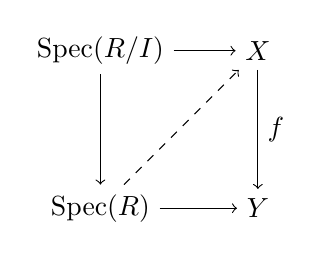
\begin{tikzpicture}
                \node (X) at (0, 1) {$X$};
                \node (Y) at (0, -1) {$Y$};
                \node (R) at (-2, -1) {$\mathrm{Spec}(R)$};
                \node (RI) at (-2, 1) {$\mathrm{Spec}(R/I)$};
                \draw[->] (X) -- node[right]{$f$} (Y);
                \draw[->] (RI) -- (X);
                \draw[->] (R) -- (Y);
                \draw[->] (RI) -- (R);
                \draw[->, dashed] (R) -- (X);
            \end{tikzpicture}
        \end{gather*}
        In other words, formally \'etale morphisms have the unique right lifting property with respect to infinitesimal thickenings. Analogously to the case of rings, the morphism $f$ is said to be \textbf{formally smooth} (resp.~\textbf{formally unramified}) if there is at least (resp.~at most) one lift.

        Since this definition does allow for some pathological examples, \'etale morphisms are defined as those morphisms that are formally \'etale and locally of finite presentation. (Likewise for smooth and unramified morphisms.)
    }

    \sremark{The term 'formally' should be interpreted in the sense of \textit{formal geometry} (see \labelref{chapter:hdg}). There, infinitesimal neighbourhoods of points (see \cref{hdg:infinitesimal_thickening}), used for defining the local geometry, are induced by nilpotent ideals. This is further exemplified by \cref{alggeom:tangent_cone_etale}.}

    \begin{property}[Equivalent conditions]
        The following conditions are equivalent for a scheme morphism $f:X\rightarrow Y$ locally of finite presentation:
        \begin{itemize}
            \item $f$ is \'etale,
            \item $f$ is flat and unramified,
            \item $f$ is flat and smooth, and
            \item $f$ is smooth and of relative dimension 0.
        \end{itemize}
        \todo{ADD Jacobian condition (see e.g.~\citet{mumford_red_1999})}
    \end{property}
    \begin{property}[Fibres]
        An \'etale morphism has discrete fibres.\footnote{This actually holds for all unramified morphisms.} In particular, if it is quasicompact, it has finite fibres.
    \end{property}

    \begin{remark}\label{alggeom:etale_remark}
        As a side note, the general definition of \'etale morphism is related to \cref{alggeom:etale_morphism_variety}. The completion of the local ring $\mathcal{O}_x$ is defined by the inverse limit over the filtration $\mathcal{O}_x/\mathfrak{m}_x\leftarrow\mathcal{O}_x/\mathfrak{m}_x^2\leftarrow\mathcal{O}_x/\mathfrak{m}_x^3\leftarrow\cdots$. Hence, a morphism $\widehat{\mathcal{O}}_x\rightarrow\widehat{\mathcal{O}}_y$ between completions is characterized by consecutive lifting problems, which are exactly the content of \cref{algebra:formally_etale}, since the ideals $\mathfrak{m}_x$ are clearly nilpotent in rings of the form $\mathcal{O}_x/\mathfrak{m}_x^k$ for any $k\in\mathbb{N}_0$.
    \end{remark}
    This is generalized to schemes as follows.
    \begin{property}\label{alggeom:etale_conditions}
        If $Y$ is locally Noetherian and $f:X\rightarrow Y$ is locally of finite presentation, \'etale morphisms can also be characterized in terms of completions. $f$ is \'etale if and only if the induced morphism on completions is formally \'etale in the adic topology.

        Moreover, if $\kappa(x)\cong f^\sharp\bigl(\kappa(x)\bigr)$, $f$ is \'etale if and only if the induced morphisms of completions are isomorphisms (as in the case of affine varieties over algebraically closed fields).
    \end{property}

    \newdef{Finite \'etale morphism}{\index{etale!morphism}
        A morphism of schemes $f:X\rightarrow Y$ for which there exists a covering $\{U_i\}_{i\in I}$ of $Y$ by affine sets $U_i\equiv\mathrm{Spec}(A_i)$ such that $f^{-1}(U_i)\cong\mathrm{Spec}(B_i)$ is a free, separable $A_i$-algebra $B_i$ for all $i\in I$.
    }
    \begin{remark}[Finite \'etale covering]\index{etale!covering}
        When a finite \'etale morphism $f:X\rightarrow Y$ exists, $X$ is sometimes called a \textbf{finite \'etale cover(ing)} of $Y$. The full subcategory of the slice category $\symbfsf{Sch}/_Y$ on finite \'etale coverings is often denoted by $\symbfsf{FEt}_X$.
    \end{remark}

    \newdef{\'Etale fundamental group}{\index{fundamental group!etale}
        Consider a connected scheme $X$. The (\'etale) fundamental group $\pi_1(X)$ is the unique (up to isomorphism) profinite group \ref{topology:profinite_group} such that $\symbfsf{FEt}_X$ is equivalent to the category $\symbfsf{Fin}\,\pi_1(X)\symbfsf{Set}$ of finite of $\pi_1(X)$-sets.
    }
    \begin{remark}
        Recall \cref{topology:equivalent_categories} for topological spaces. There, a stricter set of spaces was considered with the benefit that all $\pi_1(X)$-sets could be classified. By passing to profinite groups one can formulate a classification statement in the topological setting that is virtually identical to the above one.
    \end{remark}

    The following definition is analogous to \cref{topology:proper_function}.
    \newdef{Proper morphism}{\index{proper}\index{closed}
        A scheme morphism $f:X\rightarrow Y$ satisfying
        \begin{enumerate}
            \item $X$ is separated as a $Y$-scheme,
            \item $f$ is of finite type, and
            \item $f$ is \textbf{universally closed}, i.e.~the pullback along any scheme morphism is closed.
        \end{enumerate}
    }

\subsection{Subschemes}

    Since general schemes need not be reduced, the structure sheaf could have nilpotent sections. Consequently, restricting a structure sheaf $\mathcal{O}_X$ along a topological inclusion $Y\subseteq X$ is (generally) not possible, since nilpotent sections are not determined by their values at points.

    \newdef{Closed subscheme}{
        Let $(X,\mathcal{O}_X)$ be a scheme. A (closed) subscheme is defined by the following data:
        \begin{enumerate}
            \item A closed subset $Y\subseteq X$,
            \item A sheaf $\mathcal{O}_Y$ such that $(Y,\mathcal{O}_Y)$ is a scheme, and
            \item A surjection $\pi:\mathcal{O}_X\twoheadrightarrow\mathcal{O}_Y$, i.e.~a sheaf morphism whose maps on stalks are surjections.
        \end{enumerate}
    }

    \begin{property}[Ideal sheaf]\index{ideal!sheaf}
        If $\pi:X\rightarrow Y$ determines a closed subscheme, $\ker(\pi)$ is quasicoherent sheaf of ideals.
    \end{property}

    \begin{theorem}[Nullstellensatz]
        Closed subschemes of $X$ are equivalent to quasicoherent ideal sheaves on $X$.
    \end{theorem}

    \newdef{Closed immersion}{\index{immersion}
        A scheme morphism $f:X\rightarrow Y$ satisfying
        \begin{enumerate}
            \item (the underlying continuous function of) $f$ is injective,
            \item $f$ is closed, and
            \item $f^\sharp$ is a surjection.
        \end{enumerate}
    }

\subsection{Tangent space}

    \newdef{Tangent cone}{\index{tangent!cone}\index{initial!part}
        Consider an affine variety $X=V(I)$. The tangent cone to $X$ at the origin is defined as the zero locus of the `initial ideal' of $I$:
        \begin{gather}
            C_0X := V\bigl(\{f^{\text{in}}\bigm\vert f\in I\}\bigr)\,,
        \end{gather}
        where $f^{\text{in}}$ denotes the \textbf{initial part} of $f$, i.e.~the sum of the smallest degree monomials in $f$.
    }

    \newdef{Tangent space}{\index{tangent!space}
        Consider an affine variety $X$ and choose a point $x\in X$. By working in a suitable affine chart, one can assume that $x=0$. This implies that any polynomial $f\in I(X)$ has a vanishing constant term. The tangent space at $x$ is defined as follows:
        \begin{gather}
            T_xX := V\bigl(\{f^{[1]}\bigm\vert f\in I(X)\}\bigr)\,,
        \end{gather}
        where $f^{[1]}$ denotes the linear part of the polynomial $f$.
    }
    \begin{property}
        For $x=0$, one obtains that $I(0)=(x_1,\ldots,x_n)/I(X)$. Moreover, there exists a natural isomorphism
        \begin{gather}
            I(0)/I(0)^2\cong\hom_{\mathfrak{K}}(T_0X,\mathfrak{K})\,.
        \end{gather}
        The tangent space at $0$ can accordingly also be obtained as the dual of $I(0)/I(0)^2$.
    \end{property}

    It is not so hard to prove that this property can, in fact, easily be transported to arbitrary points $x\in X$ if one replaces the ideal $I(0)$ by the maximal ideal of the structure sheaf $\mathcal{O}_X$ at $x$. Therefore, one can give the following general definition.
    \newdef{Zariski tangent space}{\index{Zariski!tangent space}\label{alggeom:cotangent_space}
        Consider a scheme $X$ with structure sheaf $\mathcal{O}_X$. At every point $x\in X$, the stalk $\mathcal{O}_x$ is a local ring and, hence, has a maximal ideal $\mathfrak{m}_x$. The quotient $\mathfrak{m}_x/\mathfrak{m}_x^2$ is a vector space over the residue field $\mathcal{O}_x/\mathfrak{m}_x$. It is called the Zariski cotangent space at $x\in X$ and its algebraic dual is called the Zariski tangent space at $x\in X$.
    }

    \begin{property}[Finite-dimensionality]
        If $x\in X$ is closed, $T_xX\cong T^*_xX$.
    \end{property}

    \newdef{Regular scheme}{\index{regular!scheme}
        A (Noetherian) scheme is said to be regular or \textbf{nonsingular} if the local dimension at any point is equal to the dimension of the Zariski tangent space at that point. Equivalently, an affine variety is smooth if at every point the tangent space is isomorphic to the tangent cone.
    }

    \newadef{Tangent cone: Schemes}{\index{tangent!cone}
        Assume that $X$ is a Noetherian scheme. The tangent cone $C_xX$ is given by the spectrum of the graded ring $\mathrm{Gr}(\mathcal{O}_x)=\bigoplus_{k\in\mathbb{N}}\mathfrak{m}_x^k/\mathfrak{m}_x^{k+1}$. If $X$ is regular, the tangent cone coincides with the Zariski tangent space.
    }

    \begin{remark}[Inverse function theorem]\index{inverse function theorem}
        In the smooth setting (see \labelref{chapter:manifolds} and onwards), the inverse function theorem states that a tuple of functions forms a local coordinate system at a point if their \textit{differentials} generate the \textit{cotangent space} at that point.

        Here, the ideal $\mathfrak{m}_x$ consists of the functions vanishing at $x\in X$ and the cotangent space is given by $\mathfrak{m}_x/\mathfrak{m}_x^2$. By Nakayama's lemma~\ref{algebra:nakayama}, a tuple of elements represent `coordinate functions', i.e.~generate $\mathfrak{m}_x$, if their `differential', i.e.~their residues in the Zariski cotangent space, generate the cotangent space.

        For schemes, the inverse function theorem becomes the following. If a point $x\in X$ is regular, there exists a neighbourhood which is an (affine) variety.
    \end{remark}

    Recall \cref{alggeom:etale_morphism_variety} of \'etale morphisms of affine varieties (over algebraically closed fields) and \cref{alggeom:etale_conditions} for schemes. The following property relates these to the infinitesimal thickening point-of-view.
    \begin{property}\label{alggeom:tangent_cone_etale}
        A morphism $f:X\rightarrow Y$ of finite type of Noetherian schemes is \'etale if and only if it induces an isomorphism on tangent cones.
    \end{property}

    \begin{property}
        If $X$ is a scheme over a field $\mathfrak{K}$ and $x\in X$ is closed, the tangent space at $x$ admits an `alternative' description:
        \begin{gather}
            T_xX \cong \symbfsf{Sch}_{\mathfrak{K}}\left(\spec(\mathfrak{K}[\varepsilon]/\varepsilon^2),X\right)\,.
        \end{gather}
    \end{property}

    \begin{property}[Dimension]
        If $X$ is (locally) Noetherian, then
        \begin{gather}
            \dim(T_xX)\geq\dim(X)\,.
        \end{gather}
    \end{property}

\subsection{Algebraic de Rham complex}\index{de Rham!complex}

    For this section, the notion of \textit{K\"ahler differential} is used (see \cref{nca:kahler_differential}). For an affine scheme $X\equiv\mathrm{Spec}(R)$, where $R$ is finitely generated over $\mathfrak{K}$, let $\Omega_{X/\mathfrak{K}}$ denote the algebra of K\"ahler differentials. If $X$ is smooth, $\Omega_{X/\mathfrak{K}}$ will be locally free of rank $\dim(X)$.

    In a relative setting, one obtains the relative K\"ahler differentials $\Omega_{R/S}$ induced by the multiplication $\mu:R\otimes_SR\rightarrow R$. Globalizing leads to the diagonal morphism $\Delta:X\rightarrow X\times_YX$ which gives a closed subscheme $\Delta(X)$. By the Nullstellensatz, every closed subscheme is induced by a quasicoherent sheaf of ideals $\mathcal{I}$. Repeating the construction of K\"ahler differentials, one can construct the (quasicoherent) sheaf $\mathcal{I}/\mathcal{I}^2$.

    \newdef{Conormal sheaf}{\index{conormal!sheaf}
        Let $f:X\rightarrow Y$ be a scheme morphism. The conormal sheaf $\Omega_{X/Y}$ is defined as the pullback $\Delta^*(\mathcal{I}/\mathcal{I}^2)$.
    }

    The differential $\dr$ on $\Omega_{X/Y}$ can be defined by pullback as well:
    \begin{gather}
        \dr:\mathcal{O}_X\rightarrow\Omega_{X/Y}:f\mapsto\Delta^*(\pi_2^*f-\pi_1^*f)\,,
    \end{gather}
    where $\pi_1,\pi_2:X\times_YX\rightarrow X$ are the canonical projections. This derivation is $\mathcal{O}_Y$-linear.

    \begin{property}
        If $X\rightarrow Y$ is locally of finite type and $X$ is locally Noetherian, $\Omega_{X/Y}$ is coherent.
    \end{property}

    \begin{property}[Pullback stability]
        Consider the pullback $X':=Y'\otimes YX$. There exists an isomorphism
        \begin{gather}
            \pi_X^*\Omega_{X/Y}\cong\Omega_{X'/Y'}\,. 
        \end{gather}
    \end{property}
    \begin{result}
        The sheaf of differentials on a fibre coincides with the fibre of the sheaf of differentials. 
    \end{result}

    Recall \cref{alggeom:cotangent_space}. This space can be obtained by taking fibres.
    \begin{property}[Cotangent space]\index{Zariski!tangent space}
        The cotangent space at a point $x\in X$ of a scheme $X\rightarrow Y$ is equal to
        \begin{gather}
            T_x^*X = \Omega_{X/Y,x}\otimes_{\mathcal{O}_{X,x}}\kappa(x)\,.
        \end{gather}
    \end{property}

    \todo{COMPLETE}

\section{\difficult{Topos theory}}

    This section also uses the content of \labelref{chapter:topos}.

    \newdef{Zariski topology}{\index{Zariski!topology}
        The Zariski topology on the category of schemes is generated by sets $\{f_i:U_i\rightarrow X\}_{i\in I}$ of open immersions such that $X=\bigcup_{i\in I}f_i(U_i)$ in the set-theoretic sense. This latter condition is often called \textbf{joint surjectivity}. This gives the \textbf{big Zariski site} on an a scheme $X$. The \textbf{small Zariski site} of a scheme $X$ is the subsite of $\symbfsf{Sch}_{/X}$ on the open immersions.
    }
    \begin{remark}[Size issues]
        There are some size issues with the category of schemes, it being a big category. The result is that in general there exists no sheafification functor, i.e.~no general construction of the category of sheaves and, hence, this category can only be turned into a site, not a (Grothendieck) topos.\footnote{One can actually also work with large sites to obtain topoi as long as they contain a \textit{small topologically generating set} or, even more general, satisfy the \textit{WISC axiom}.} In the case of \textit{topological} or \textit{smooth manifolds}, this problem is often ignored since one has a (small) dense subsite and no issues arise. For schemes, however, the situation is different. For example, the fpqc topology (to be introduced below) does not admit a sheafification functor. Two solutions exists in such a context, either one works within a suitable universe or one only considers a single (pre)sheaf at a time.
    \end{remark}

    \begin{property}
        The Zariski site is subcanonical.
    \end{property}

    The following topology is finer than the Zariski topology.\footnote{There exists another topology in between the Zariski and \'etale topologies, the \textit{Nisnevich topology}, but this is of no interest here.}
    \newdef{\'Etale cover}{\index{cover!\'etale}\index{site!\'etale}
        An \'etale cover of a scheme $X$ is a jointly surjective family of \'etale morphisms that are locally of finite type\footnote{For $X$ locally Noetherian, this additional condition is superfluous.}. The \textbf{big \'etale site} $\symbfsf{Sch}_{/X,\text{\'et}}$ is the slice category of $X$ equipped with the coverage (see \cref{topos:coverage}) of \'etale covers. The \textbf{small \'etale site} is the subsite on \'etale morphisms.
    }

    \begin{property}
        A presheaf satisfies descent with respect to the \'etale topology if and only if it satisfies descent with respect to the following covers:
        \begin{itemize}
            \item Zariski covers, and
            \item (single) faithully flat morphisms of affine schemes.
        \end{itemize}
    \end{property}

    \newdef{Flat topologies}{\index{flat!topology}
        The finest topologies on the category of schemes (or slices thereof) are given by considering flat morphisms. The two most widely used flat topologies are the `fppf-' and `fpqc-topologies'. The \textbf{fppf-topology} (for \textit{fid\`element plat de presentation finie}) is generated by jointly surjective families of flat morphisms that are locally of finite presentation. The \textbf{fpqc-topology} (for \textit{fid\`element plat et quasi-compacte}) is generated by jointly surjective families of flat and quasicompact morphisms.
    }
    \begin{remark}
        As defined above, the fpqc-topology is technically not comparable to the Zariski topology, since open immersions need not be quasicompact (unless one restricts to Noetherian schemes). A solution introduced by \indexauthor{Vistoli} and \indexauthor{Kleiman} is to replace quasicompactness by the following seemingly similar definition: There exists an open affine cover $\{U_i\}_{i\in I}$ of $X$ such that each $U_i$ is the image of a compact open subscheme. (If one drops the modifier `locally' in the definition of the fppf-topology, a similar problem arises.)
    \end{remark}
    \begin{remark}[Standard covers]
        An equivalent approach to the definition of flat topologies is by first defining `standard' fppf or fpqc covers on affine schemes. These are similar to the flat covers defined above, but where the families are finite and the codomains affine. The covers of general schemes are then generated by base change.
    \end{remark}

    By interpreting objects in the big topos (over a scheme) as generalized spaces in the sense of \labelref{chapter:hdg}, the following definition is obtained.
    \newdef{Algebraic space}{\index{algebraic!space}\index{atlas}\label{alggeom:algebraic_space}
        An object $X\in\symbfsf{Sh}(\symbfsf{Sch}_{\text{fppf}})$ satisfying
        \begin{enumerate}
            \item The diagonal morphism $X\rightarrow X\times X$ is \textit{representable} (see \cref{topos:representable_diagonal}).
            \item There exists a scheme morphism $Y\rightarrow X$ that is surjective and \'etale. This is sometimes called an \textbf{atlas}.
        \end{enumerate}
        Requiring representability of the diagonal can be argued as follows. The fibre product can be seen as a generalized notion of intersection, so representability means that the intersection of any two schemes is again a scheme. Moreover, representability of the diagonal also implies representability of the atlas.
    }

    \newdef{Local property}{\index{local!property}\label{alggeom:local_property}
        Consider some property of scheme morphisms $P$, e.g.~\'etale or smoothness. Relative to some topology on $\symbfsf{Sch}$, the property $P$ is said to be \textbf{local on the source} if for every cover $\{X_i\rightarrow X\}_{i\in I}$ and every morphism $f:X\rightarrow Y$ the following holds:
        \begin{gather}
            f\text{ satisfies }P\iff\forall i\in I:X_i\rightarrow Y\text{ satisfies }P\,.
        \end{gather}
        Analogously, the property $P$ is said to be \textbf{local on the base} or \textbf{local on the target} if for every cover $\{Y_i\rightarrow Y\}_{i\in I}$ and every morphism $f:X\rightarrow Y$ the following holds:
        \begin{gather}
            f\text{ satisfies }P\iff\forall i\in I:Y_i\times_YX\rightarrow Y_i\text{ satisfies }P\,.
        \end{gather}
    }

    Inspired by locality, one can generalize many properties of scheme morphisms to morphisms of algebraic spaces.
    \newdef{Property of algebraic spaces}{
        Consider a representable morphism of algebraic spaces $F:X\rightarrow Y$. If $P$ is a property of scheme morphisms satisfying:
        \begin{enumerate}
            \item it is preserved under base change, and
            \item it is fppf-local on the target,
        \end{enumerate}
        then $f$ is said to have the property $P$ if for all $T\in\ob{Sch}$ and all $G:h_T\rightarrow Y$ the morphism $S_G\rightarrow T$ has property $P$, where $S_G\in\ob{Sch}$ is a representing object of $G$, i.e.~$h_{S_G}\cong h_T\times_YF$.
    }
    \newdef{\'Etale morphism}{\index{etale!morphism}
        A morphism $F:X\rightarrow Y$ of algebraic spaces such that for every \'etale morphism $G:h_S\rightarrow X$ the composition $f\circ g$ is also \'etale.\footnote{In a similar vein, one can define smooth morphisms of algebraic spaces.}
    }

\section{Algebraic groups \& Galois theory}\index{Galois!theory}

    For some background on Galois theory, see \labelref{section:galois_extensions}.

\subsection{Weil restriction}

    Consider a $\mathfrak{K}$-variety $X\rightarrow\spec(\mathfrak{K})$ such that $X$ is characterized by polynomials with coefficients in a subfield $\mathfrak{K}_0$. In this case, one has
    \begin{gather}
        X\cong\spec\left(\mathfrak{K}_0[x_1,\ldots,x_n]/I_0\right)\times_{\spec(\mathfrak{K}_0)}\spec(K)\,.
    \end{gather}
    Such a variety $X$ is said to be \textbf{defined over $\mathfrak{K}_0$}. (This also works for schemes.)

    A related notion is the following.
    \newdef{Weil restriction}{\index{Weil!restriction}\index{restriction!of scalars}
        Consider an $\mathfrak{L}$-scheme $X$ together with a field extension $\mathfrak{L}/\mathfrak{K}$. One can obtain a $\mathfrak{K}$-scheme by \textbf{restriction of scalars}\footnote{This adjunction is inherited from an adjunction on rings.}:
        \begin{gather}
            \symbfsf{Sch}_{\mathfrak{K}}\left(S,\mathrm{Res}_{\mathfrak{L}/\mathfrak{K}}X\right) := \symbfsf{Sch}_{\mathfrak{L}}\left(S\times_{\spec(\mathfrak{K})}\mathfrak{L},X\right)\,.
        \end{gather}
    }
    
    Now, consider a field extension $\mathfrak{L}/\mathfrak{K}$ and a $\mathfrak{K}$-scheme $X$. From this, one can construct an $\mathfrak{L}$-scheme as above by base change:
    \begin{gather}
        \widetilde{X} := X\times_{\mathfrak{K}}\spec(\mathfrak{L})\,.
    \end{gather}
    Every automorphism $\sigma\in\Aut(\mathfrak{K}/\mathfrak{L})$ induces an automorphism on $\widetilde{X}$. Note that, on the unique stalk of the affine factor, $f^*=\sigma^{-1}$ by contravariance.

    \begin{property}[Galois action]
        If $\mathfrak{L}=\overline{\mathfrak{K}}$, the fibre $\pi^{-1}(x)$, with respect to the projection $\pi:\widetilde{X}\rightarrow X$, is a finite orbit of the $\Aut(\overline{\mathfrak{K}}/\mathfrak{K})$-action. In fact,
        \begin{gather}
            X \cong \widetilde{X}/\Aut(\overline{\mathfrak{K}}/\mathfrak{K})
        \end{gather}
        as topological spaces.
    \end{property}
    \begin{remark}[Ambient category]
        As schemes, the quotient above is not isomorphic to $X$. One needs more, such as $\mathfrak{K}$ being perfect (\cref{algebra:perfect_field}), hence working with Galois extensions, and $X$ being reduced.
    \end{remark}

    \begin{remark}[Galois descent]\index{Galois!descent}\index{form}
        Although only a small introduction to the topic was presented here, a vast amount of work exists on recovering subschemes from Galois actions (and beyond). The keywords here are `\textit{forms}' and `\textit{Galois descent}' (see e.g.~\citet{milne_descent_2024}).
    \end{remark}

\subsection{Galois theory}

    \begin{property}[Fixed points]
        When $\mathfrak{K}$ is perfect, the fixed points of $\mathrm{Gal}(\mathfrak{L}/\mathfrak{K})$ correspond to the $\mathfrak{K}$-rational points of the form $\pi(x)$ for $x\in\widetilde{X}$.
    \end{property}

    \newdef{Absolute Galois group}{
        The Galois group $\mathrm{Gal}(\mathfrak{K}_S/\mathfrak{K})$ of the separable closure (\cref{algebra:separable_closure}) of $\mathfrak{K}$.
    }

    The following property relates Galois theory to algebraic geometry.
    \begin{property}[Grothendieck's Galois theory]\index{Grothendieck}
        Consider a field $\mathfrak{K}$ with separable closure $\mathfrak{K}_S$.
        \begin{gather}
            \mathrm{Gal}(\mathfrak{K}_S/\mathfrak{K})\cong\pi_1\bigl(\mathrm{Spec}(\mathfrak{K})\bigr)\,,
        \end{gather}
        where $\pi_1$ is the \'etale fundamental group (the fundamental group at the topological level would not carry a lot of information since $\mathrm{Spec}(\mathfrak{K})$ is a one-point space).
    \end{property}

    

    \newdef{Group scheme}{\index{group!scheme}
        A group object in $\symbfsf{Sch}$.
    }
    \begin{example}[Additive group]\index{group!additive}
        The additive group $\mathbb{G}_a$ (over some field $\mathfrak{K}$) has as underlying object the affine line $\spec(\mathfrak{K}[x])$ and as operations:
        \begin{enumerate}
            \item\textbf{Addition}: Dual of the ring morphism $\mathfrak{K}[x]\rightarrow \mathfrak{K}[x_1]\otimes \mathfrak{K}[x_2]:x\mapsto x_1+x_2$.
            \item\textbf{Unit}: Dual of $\mathfrak{K}[x]\rightarrow\mathbb{Z}:x\mapsto0$.
            \item\textbf{Inversion}: Dual of $\mathfrak{K}[x]\rightarrow \mathfrak{K}[x]:x\mapsto-x$.
        \end{enumerate}
        Equivalently, it is the $\symbfsf{Ab}$-valued functor that sends a scheme to the Abelian group of global sections of its structure sheaf.
    \end{example}

    \newdef{Linear algebraic group}{\index{group!algebraic}
        A subgroup of $\GL(n,\mathfrak{K})$ defined by a (finite) set of polynomials in the matrix coefficients.
    }
    \begin{property}
        From the definition, it is immediately clear that intersections of algebraic groups are again algebraic.
    \end{property}

    \newdef{Abelian variety}{\index{variety!Abelian}\label{alggeom:abelian_variety}
        A smooth, projective and algebraic group.
    }
    \begin{theorem}[Mordell--Weil]
        For an Abelian variety $X$ over a number field $\mathfrak{K}$ (\cref{algebra:number_field}), the set of rational points $X(\mathfrak{K})$ (\cref{alggeom:rational_point_scheme}) is a finitely generated Abelian group.
    \end{theorem}

\section{Tropical geometry}\index{tropical geometry}

    The following definition generalizes \cref{group:ring}.
    \newdef{Rig}{\index{rig}
        Let $R$ be a set equipped with two binary operations $+,\cdot$ (called\footnote{This might become confusing when looking at the examples below.} \textbf{addition} and \textbf{multiplication}). $(R,+,\cdot)$ is a rig if it satisfies the following axioms:
        \begin{enumerate}
            \item $(R,+)$ is a commutative monoid.
            \item $(R,\cdot)$ is a monoid.
            \item Multiplication is distributive with respect to addition.
        \end{enumerate}
    }
    \begin{remark}
        Whereas a ring is a group object in $\symbfsf{CRing}$, a rig is a group object in $\symbfsf{CMonoid}$. (The monoidal structures on these categories should not be taken to be the Cartesian ones for this result).
    \end{remark}

    \begin{example}[Tropical rig]
        Consider the set $T:=\mathbb{R}\cup\{+\infty\}$. This set becomes a rig when equipped with the following operations:
        \begin{enumerate}
            \item\textbf{Addition}: $x\oplus y=\min(x,y)$.
            \item\textbf{Multiplication}: $x\cdot y=x+y$.
        \end{enumerate}
    \end{example}

    \newdef{Tropicalization}{\index{tropicalization}\index{Puiseux series}
        In ordinary algebraic geometry, one considers polynomials over $\mathbb{R}$ as the basic building blocks. These also give rise to polynomials over $T$. To every polynomial
        \begin{gather}
            f = a+\sum_{i=1}^k\lambda_ix^{n_i}_i
        \end{gather}
        with $a\in\mathbb{Z}$, one assigns its tropicalization
        \begin{gather}
            \mathrm{trop}(f) := \min(0,n_1x_1,\ldots,n_kx_k)\,.
        \end{gather}
        Note that the tropicalization of any polynomial is a piecewise linear function.

        A more formal definition goes as follows. Let $\mathfrak{K}_P$ be the ring of \textbf{Puiseux series}, i.e.~of elements of the form
        \begin{gather}
            a = \sum_{i=k}^{+\infty}\lambda_ix^{i/n}
        \end{gather}
        for some $k,n\in\mathbb{N}$. These generalize Laurent series (\cref{complex:laurent_series}) to fractional exponents in that $\mathfrak{K}_P=\bigcup_{i\in\mathbb{N}_0}\mathbb{C}((x^{1/i}))$. Then, consider the valuation (\cref{algebra:valuation})
        \begin{gather}
            \mathrm{val}:\mathfrak{K}_P\rightarrow\mathbb{R}:a\mapsto\min\{i/k\mid\lambda_i\neq0\}\,.
        \end{gather}
        The tropicalization of
        \begin{gather}
            f = \sum_{u\in\mathbb{N}^n}\lambda_ux^u
        \end{gather}
        with $n\in\mathbb{N}$ is given by
        \begin{gather}
            \mathrm{trop}(f) := \min_{u\in\mathbb{N}^n,\lambda_u\neq 0}\bigl(\mathrm{val}(\lambda_u)+\sum_{i=1}^nu_ix_i\bigr)\,.
        \end{gather}
    }

    \todo{COMPLETE (link with mirror symmetry \citep{gross_tropical_2011})}
% \chapter{Number Theory}

    \minitoc

\section{Adic numbers}

    This section will make use of the content of \cref{section:stone_spaces}.

    \newdef{$p$-adic numbers}{\index{adic numbers}
        Consider a prime number $p\in\mathbb{N}$. For every $m,n\in\mathbb{N}$, one has that $\mathbb{Z}/p^n\mathbb{Z}\subseteq\mathbb{Z}/p^m\mathbb{Z}$ whenever $m\leq n$. The group $\mathbb{Z}_p$ of \textbf{$p$-adic integers} is given by the profinite group (\cref{topology:profinite_group}) obtained from this system of inclusions.

        Just like $\mathbb{Q}$ is the field of fractions (\cref{algebra:fraction_field}) of $\mathbb{Z}$ as in \cref{algebra:integers_rationals}, the $p$-adic numbers $\mathbb{Q}_p$ can be obtained as the field of fractions of $\mathbb{Z}_p$.
    }

    An alternative definition makes use of the notion of valuations (\cref{algebra:valuation}).
    \newadef{$p$-adic numbers}{\index{absolute value}
        Consider a prime number $p\in\mathbb{N}$. The $p$-adic valuation of an integer $z\in\mathbb{Z}$ is defined as follows:
        \begin{gather}
            \nu_p(z) :=
            \begin{cases}
                \max\{n\in\mathbb{N}:p^n\mid z\}&\cif z\neq0\,,\\
                +\infty&\cif z=0\,.
            \end{cases}
        \end{gather}
        This valuation extends to the rational numbers by taking
        \begin{gather}
            \nu_p\left(\frac{a}{b}\right) := \nu_p(a)-\nu_p(b)\,.
        \end{gather}
        In turn, the $p$-adic valuation also induces an \textit{absolute value} on $\mathbb{Z}$ (and on $\mathbb{Q}$) given by
        \begin{gather}
            |z|_p := p^{-\nu_p(z)}\,.
        \end{gather}
        The metric completions of $\mathbb{Z}$ and $\mathbb{Q}$ by these absolute values are the rings of $p$-adic integers and numbers, respectively.
    }
    \begin{remark}
        The $p$-adic valuation of a rational number $q\in\mathbb{Q}$ can also be defined as the (unique) integer $k\in\mathbb{Z}$ such that
        \begin{gather}
            q = p^k\frac{m}{n}
        \end{gather}
        for some integers $m,n\in\mathbb{Z}$ such that $p^k$, $m$ and $n$ are all coprime.
    \end{remark}

    \begin{theorem}[Ostrowski]\index{Ostrowski}
        The only nontrivial absolute values on $\mathbb{Q}$ are either the ordinary absolute value $|\cdot|$ or the $p$-adic absolute values $|\cdot|_p$.
    \end{theorem}

    \newdef{Profinite integers}{\index{integer!profinite}
        Similar to the construction of the $p$-adic integers, one can also construct the profinite completion (\cref{topology:profinite_completion}) of $\mathbb{Z}$. Instead of taking the inverse limit over the integers module a prime power, one simply takes the inverse limit over all finite cyclic groups:
        \begin{gather}
            \widehat{\mathbb{Z}} := \varprojlim_{n\in\mathbb{N}}\mathbb{Z}/n\mathbb{Z}\,.
        \end{gather}
        It can be shown that this is equivalent to taking the product of all $p$-adic integers:
        \begin{gather}
            \widehat{\mathbb{Z}}\cong\prod_{p\text{ is prime}}\mathbb{Z}_p\,.
        \end{gather}
    }

    \newdef{Adeles}{\index{adele}
        The ring of integral adeles is defined as the product
        \begin{gather}
            \mathbb{A}_{\mathbb{R}} := \mathbb{R}\times\widehat{\mathbb{Z}}\,.
        \end{gather}
        To obtain the proper ring of adeles, the above ring is rationalized:
        \begin{gather}
            \mathbb{A}_{\mathbb{Q}} := \mathbb{Q}\otimes_{\mathbb{Z}}\mathbb{A}_{\mathbb{R}}\,.
        \end{gather}
    }

\section{\difficult{Algebraic geometry}}

    This section gives a relation between number theory and (algebraic) geometry (\cref{chapter:alggeom}). The content of \namecrefs{chapter:complexcalculus}~\ref{chapter:algebra} and~\ref{chapter:complexcalculus} will also be used throughout this section.

\subsection{Modular forms}

    \newdef{Modular group}{\index{modular!group}\index{M\"obius transformation}\label{alggeom:modular_group}
        In the setting of number theory, the projective special linear group $\mathrm{PSL}(2,\mathbb{Z})$ is often called the modular group. The modular group acts on the complex plane by \textbf{M\"obius transformations}:
        \begin{gather}
            \begin{pmatrix}
                a&b\\
                c&d
            \end{pmatrix}
            z := \frac{az+b}{cz+d}\,.
        \end{gather}
        For this reason, $\mathrm{PSL}(2,\mathbb{C})$ is sometimes also called the \textbf{M\"obius group}.
    }

    \newdef{Modular form}{\index{modular!form}\index{cusp form}
        A modular form of weight $k\in\mathbb{R}$ is a holomorphic function on the upper-half plane $f:\mathcal{H}\rightarrow\mathbb{C}$ satisfying the following two conditions:
        \begin{enumerate}
            \item\textbf{Automorphicity}: For all $g\equiv\begin{pmatrix}a&b\\c&d\end{pmatrix}\in\mathrm{PSL}(2,\mathbb{Z})$, one has $f\bigl(g(z)\bigr)=(cz+d)^kf(z)$, and
            \item\textbf{Bounded growth}: $f(z)$ is bounded for $z\longrightarrow i\infty$.
        \end{enumerate}
        If the modular form satisfies the stronger condition $f(z)\longrightarrow0$ when $z\longrightarrow i\infty$, it is said to be \textbf{cuspidal} or it is simply called a \textbf{cusp form}.
    }
    \begin{remark}[Arithmetic group]\index{arithmetic group}
        Modular forms can also be defined for subgroups of $\mathrm{PSL}(2,\mathbb{Z})$ with finite index, the so-called \textbf{arithmetic groups}.
    \end{remark}

    \begin{property}
        The generators of the modular group are given by
        \begin{gather}
            z\mapsto-\frac{1}{z}\qquad\text{and}\qquad z\mapsto z+1\,.
        \end{gather}
        Invariance under the second generator shows that modular forms are, in particular, periodic and, hence, admit a Fourier expansion. Cusp forms are exactly those modular forms with vanishing constant Fourier coefficient.
    \end{property}

\subsection{Algebraic functions}

    \Cref{algebra:algebraic_element} can be generalized to the functional setting.
    \newdef{Algebraic function}{\index{algebraic!function}\index{transcendental!function}
        Let $R$ be a commutative ring. A function $f:R^n\rightarrow R$ is said to be algebraic if it is the solution of a polynomial equation with coefficients in $R[x_1,\ldots,x_n]$.\footnote{Often, the polynomial is required to be irreducible.} If $f$ is not algebraic, it is said to be \textbf{transcendental}.
    }

% \part{Higher Set Theory}
% \insertparttoc

% \chapter{Topos theory}\label{chapter:topos}

    The main reference for this chapter is~\citet{johnstone_topos_2014,caramello_lectures_2019,caramello_topos-theoretic_2018,mac_lane_sheaves_1994}. For an introduction to stacks and descent theory, see~\citet{vistoli_notes_2004}.

    \minitoc

\section{Elementary topoi}

    \newdef{Subobject classifier}{\index{subobject!classifier}
        Consider a finitely complete category (in fact, the existence of a terminal object suffices). A subobject classifier is a mono\footnote{The symbol for this morphism will become clear in \cref{section:internal_logic}.} $\texttt{true}:1\hookrightarrow\Omega$ from the terminal object such that for every mono $\phi:x\hookrightarrow y$ there exists a unique morphism $\chi:y\rightarrow\Omega$ that fits in the following pullback square:
        \begin{figure}[ht!]
            \centering
            \begin{tikzpicture}
                \node (A) at (0, 0) {$x$};
                \node (B) at (0, -2) {$y$};
                \node (1) at (2, 0) {$1$};
                \node (O) at (2, -2) {$\Omega$};
                \node at (1, -1) {pb};
                \draw[->] (A) -- (1);
                \draw[right hook->] (A) -- node[left]{$\phi$} (B);
                \draw[right hook->] (1) -- node[right]{$\texttt{true}$} (O);
                \draw[->] (B) -- node[below]{$\exists!\chi$} (O);
            \end{tikzpicture}
            \caption{Subobject classifier.}
            \label{fig:subobject_classifier}
        \end{figure}
    }
    \begin{adefinition}
        Consider a well-powered category $\symbfsf{C}$. The assignment of subobjects $\mathrm{Sub}(x)$ to an object $x\in\ob{C}$ defines functor $\mathrm{Sub}:\symbfsf{C}^{op}\rightarrow\symbfsf{Set}$. A subobject classifier $\Omega$ is a representation of this functor, i.e.~the following isomorphism is natural in $x$:
        \begin{gather}
            \mathrm{Sub}(x)\cong\symbfsf{C}(x,\Omega)\,.
        \end{gather}
    \end{adefinition}

    \begin{example}[Indicator function]\index{indicator function}
        The category $\symbfsf{Set}$ has the 2-element set $\{\texttt{true},\texttt{false}\}$ as subobject classifier. The morphism $\chi:S\rightarrow\Omega$ is the indicator function
        \begin{gather}
            \chi_S(x)=
            \begin{cases}
                \texttt{true}&\cif x\in S\,,\\
                \texttt{false}&\cif x\not\in S\,.
            \end{cases}
        \end{gather}
    \end{example}

    \newdef{Elementary topos}{\index{topos!elementary}
        An elementary topos is a finitely complete, Cartesian closed category (\cref{cat:closed}) admitting a subobject classifier. Equivalently, one can define an elementary topos as a finitely complete category that has all power objects exist.

        The power object $Px$ of $x\in\ob{\mathcal{E}}$ is related to the subobject classifier $\Omega$ by the following relation:
        \begin{gather}
            \label{topos:power_exponential}
            Px = \Omega^x\,.
        \end{gather}
    }
    \begin{remark}[Finite colimits]
        The original definition by \textit{Lawvere} also required the existence of finite colimits. However, it can be proven that finite cocompleteness follows from the other axioms.
    \end{remark}

    \begin{theorem}[Fundamental theorem of topos theory]\index{fundamental theorem!of topos theory}
        Let $\mathcal{E}$ be an elementary topos. The slice category $\mathcal{E}_{/x}$ is also a topos for every object $x\in\ob{\mathcal{E}}$. The subobject classifier is given by $\pi_2:\Omega\times x\rightarrow x$.
    \end{theorem}

    \begin{property}[Balanced]
        All monos in a topos are regular. Hence, every mono arises as an equalizer. Since, by \cref{cat:regular_iso}, every epic equalizer is necessarily an isomorphism, it follows that every topos is balanced (\cref{cat:balanced}).
    \end{property}

    \begin{property}[Epi/mono factorization]\index{image}
        Every morphism $f:x\rightarrow y$ in a topos factorizes uniquely as an epi followed by a mono:
        \begin{gather}
            x\overset{e}{\twoheadrightarrow}z\overset{m}{\hookrightarrow}y\,.
        \end{gather}
        The mono is called the \textbf{image} of $f$.
    \end{property}

\section{Morphisms}

    \newdef{Base change}{\index{base change}\label{topos:base_change}
        Consider a category $\symbfsf{C}$ with pullbacks. For every morphism $f:x\rightarrow y$ one can define a functor $f^*:\symbfsf{C}/y\rightarrow\symbfsf{C}/x$. This functor acts by pullback along $f$.
    }
    \newdef{Dependent sum and product}{\index{dependent!sum/product}\label{topos:dependent_functors}
        Consider a base change functor $f^*$. The dependent sum and product functors are given by the right and left adjoints (if they exist):
        \begin{gather}
            \label{topos:dependent_adjoint_triple}
            \sum_f\dashv f^*\dashv \prod_f\,.
        \end{gather}
    }
    \begin{remark}
        The dependent sum can be shown to exist over any category. In fact, as a functor, it is simply given by postcomposition with $f$. However, the interpretation is much less trivial. Any morphism can be interpreted as a ``space'' with fibres the preimages. For example, in $\symbfsf{Set}$, a morphism $g:Z\rightarrow X$ represents $Z$ as follows: \[Z\cong\bigsqcup_{x\in X}g^{-1}(x)\equiv\sum_{x:X}g^{-1}(x).\] The dependent sum generalizes this construction in a fibrewise manner, i.e.~the fibre over a point $y\in Y$ is given by
        \begin{gather}
            \sum_fg\,\Big|_y = \bigsqcup_{x\in f^{-1}(y)}g^{-1}(x)\,.
        \end{gather}
        Instead of combining all fibres into a single space, it combines those that lie in a single fibre of $f$.
    \end{remark}

    Although the dependent sum always exists, the dependent product requires more structure (see e.g.~\citet{huang_locally_2022}).
    \begin{property}[Locally Cartesian closed categories]
        In a locally Cartesian closed category (\cref{cat:closed}), all dependent products exist. In fact, the existence of the adjoint triple~\eqref{topos:dependent_adjoint_triple} is equivalent to $\symbfsf{C}$ being locally Cartesian closed. For example, in $\symbfsf{Set}$, the dependent product is given by
        \begin{gather}
            \label{topos:dependent_product_sets}
            \prod_fg\,\Big|_y=\prod_{x\in f^{-1}(y)}g^{-1}(x)\,.
        \end{gather}
        When $f$ is the terminal morphism, this represents the space of sections $X\rightarrow Z\equiv\sum_{x:X}g^{-1}(x)$ of $g$.

        More generally, the functor is obtained through the product-exponential adjunction in slice categories. The pullback is equal to a product in a slice category. Since $\symbfsf{C}$ is locally Cartesian, one obtains for all $p:a\rightarrow y$ and $q:b\rightarrow y$:
        \begin{gather}
            \symbfsf{C}_{/x}(p\times f,q)\cong\symbfsf{C}_{/y}(p,q^f)
        \end{gather}
        for some morphism $q^f:b^f\rightarrow y$. Applying this exponential functor to the identity morphism $\mathbbm{1}_f$, gives a morphism $s:\mathbbm{1}_y\rightarrow f^f$ or $s:y\rightarrow x^f$ (this simply picks out the identity morphism in the exponential object internally). The dependent product is then defined as the pullback $\prod_fg:=s^*g^f$, where $g^f$ is interpreted as the morphism $(f\circ g)^f\rightarrow f^f$ in $\symbfsf{C}_{/y}$.

        The idea behind this pullback construction is that in $\symbfsf{Set}$, the pullback of $g^X:Z^X\rightarrow X^X$ along $s:\mathbbm{1}_X\rightarrow X^X$ is equal to the set
        \begin{gather}
            \{h\in Z^X\mid h\circ g=\mathbbm{1}_Z\}\,,
        \end{gather}
        i.e.~it consists of all sections of $g$. Hence, the pullback construction generalizes \cref{topos:dependent_product_sets}.
    \end{property}

    \newdef{Logical morphism}{\index{morphism!logical}
        A functor $f:\mathcal{E}\rightarrow\mathcal{F}$ between elementary topoi is said to be logical if it preserves finite limits, exponential objects and the subobject classifier.
    }
    \begin{property}
        If a logical morphism has a left adjoint if and only if it has a right adjoint.
    \end{property}

    \newdef{Geometric morphism}{\index{morphism!geometric}\index{direct!image}\index{inverse!image}
        A geometric morphism $f:\mathcal{E}\rightarrow\mathcal{F}$ of elementary topoi consists of an adjunction \[\mathcal{E}\adj{f^*}{f_*}\mathcal{F}\,,\] where the left adjoint is left exact. The right adjoint $f_*$ is called the \textbf{direct image} part of $f$ and the left adjoint $f^*$ is called the \textbf{inverse image} part. If $f^*$ itself has a left adjoint, then $f$ is said to be \textbf{essential}.
    }

    \newdef{Geometric surjection}{\index{surjective}
        A geometric morphism for which the inverse image part is faithful or, equivalently, reflects isomorphisms, is said to be \textbf{surjective} or is called a geometric surjection.
    }

    \newdef{Geometric embedding}{\index{embedding}\index{sub-!topos}\index{level}\label{topos:essential_subtopos}
        A geometric morphism for which the direct image part is fully faithful. If $\mathcal{E}\hookrightarrow\mathcal{F}$ is a geometric embedding, $\mathcal{E}$ is sometimes called a \textbf{subtopos} of $\mathcal{F}$. Moreover, if it is an essential geometric morphisms, the subtopos is itself said to be \textbf{essential}. Essential subtopoi $\mathcal{E}\hookrightarrow\mathcal{F}$ are also called \textbf{levels} of $\mathcal{F}$.
    }
    \begin{property}[Characterization of geometric embeddings]\label{topos:characterization_embedding}
        Let $f:\mathcal{E}\hookrightarrow\mathcal{F}$ be a geometric embedding and let $W\subset\mathrm{hom}(\mathcal{F})$ be the collection of morphisms that are mapped to isomorphisms under $f^*$. $\mathcal{E}$ is both equivalent to the full subcategory of $\mathcal{F}$ on $W$-local objects (\cref{cat:local_object}) and the \textit{localization} $\mathcal{F}[W^{-1}]$ at $W$ (see \cref{model:localization}).
    \end{property}

    \begin{property}[Base change]\index{base change}
        The base change functors on a topos are logical and admit a left adjoint, the postcomposition functor. This implies that these functors can be refined to essential geometric morphisms.
    \end{property}

    \begin{example}[Topological spaces]\label{topos:topological_spaces}
        Every continuous function $f:X\rightarrow Y$ induces a geometric morphism
        \begin{gather}
            \symbfsf{Sh}(X)\adj{f^*}{f_*}\symbfsf{Sh}(Y)\,,
        \end{gather}
        where the direct image functor $f_*$ is defined as
        \begin{gather}
            f_*F(U) := F(f^{-1}U)
        \end{gather}
        for any sheaf $F\in\symbfsf{Sh}(X)$ and any open subset $U\in\symbfsf{Open}(Y)$. The inverse image functor $f^*$ is defined using the equivalence between sheaves on topological spaces and \'etal\'e spaces. Consider a sheaf $E\in\symbfsf{Sh}(Y)$ as an \'etal\'e space $\pi:E\rightarrow Y$. The inverse image of $E$ along a continuous function $f:X\rightarrow Y$ is the pullback of $\pi$ along $f$.
    \end{example}

    This example implies that the global elements $\ast\rightarrow X$ of a topological space induce geometric morphisms of the form $\symbfsf{Sh}(\ast)\rightarrow\symbfsf{Sh}(X)$. By noting that $\symbfsf{Sh}(\ast)=\symbfsf{Set}$, one obtains the following generalization.
    \newdef{Point}{\index{point}
        A point of a topos $\mathcal{E}$ is a geometric morphism $\symbfsf{Set}\rightarrow\mathcal{E}$.
    }

    \newnot{Category of topoi}{
        The category of elementary topoi and geometric morphisms is a 2-category. It is denoted by $\symbfsf{Topos}$.

        To obtain the structure of a 2-category, one needs to define an appropriate notion of 2-morphism. Because a geometric morphism consists of an adjunction, one can consider two distinct conventions. Either, one can choose the 2-morphisms in $\symbfsf{Topos}$ to be the natural transformations $f^*\Rightarrow g^*$ (with associated transformations $g_*\Rightarrow f_*$) or, one can choose them to be the natural transformations $f_*\Rightarrow g_*$ (and associated transformations $g^*\Rightarrow f^*$). This chapter follows~\cite{johnstone_topos_2014} and the `inverse image convention' is used, i.e.~a 2-morphism $f\Rightarrow g$ consists of natural transformations $f^*\Rightarrow g^*$ and $g_*\Rightarrow f_*$.
    }

    \begin{property}[Balanced]
        The category $\symbfsf{Topos}$ is balanced (\cref{cat:balanced}), i.e.~every geometric morphism that is both a geometric embedding and a geometric surjection is an equivalence. 
    \end{property}

    \begin{theorem}[Factorization]\index{factorization}
        Every geometric morphisms can be factorized as a geometric surjection followed by a geometric embedding.
    \end{theorem}

\section{Internal logic}\label{section:internal_logic}

    In this subsection, finitely complete categories that admit a subobject classifier are considered (they do not have to be elementary topoi).

    \newdef{Truth value}{\index{truth value}
        A global element of the subobject classifier, i.e.~a morphism $1\rightarrow\Omega$. The subobject classifier $\Omega$ is also sometimes called the \textbf{object of truth values}.
    }

    \begin{property}[Heyting algebra]\label{topos:heyting_algebra}
        For all objects $x$ in an elementary topos, the poset of subobjects $\mathrm{Sub}(x)$ has the structure of an internal meet-semilattice since forming pullbacks of monos gives a natural transformation
        \begin{gather}
            \cap_x:\hom(x,\Omega\times\Omega)\rightarrow\hom(x,\Omega)\,.
        \end{gather}
        By the Yoneda lemma, this induces an internal map
        \begin{gather}
            \land:\Omega\times\Omega\rightarrow\Omega\,.
        \end{gather}
        In fact, it can be shown that this gives the structure of an internal Heyting algebra (\cref{set:heyting}) and, in particular, that of an internal locale (\cref{topology:locale}). Hence, every topos canonically gives an external Heyting algebra, namely $\mathrm{Sub}(1)$. Furthermore, every power object is an internal Heyting algebra. This in particular includes the subobject classifier $\Omega=P1$.
    \end{property}

    \newdef{Mitchell--B\'enabou language}{\index{Mitchell--B\'enabou language}\index{proposition}\index{type}\index{variable}\index{term}
        Let $\mathcal{E}$ be an elementary topos with subobject classifier $\Omega$.
        \begin{enumerate}
            \item\textbf{Type}: An object $x\in\ob{\mathcal{E}}$.
            \item\textbf{Variable} (of type $x$): An identity morphism $\mathbbm{1}_x$.
            \item\textbf{Term} (of type $x$ in variables $\alpha_i$ of type $x_i$): a morphism $\prod_{i\in I}x_i\rightarrow x$.
            \item\textbf{Formula} or \textbf{proposition}: a term of type $\Omega$. Moreover, a formula is deemed true if it factors through $\mathtt{true}:1\rightarrow\Omega$.
        \end{enumerate}
        The logical connectives are induced by the internal Heyting structure on $\Omega$. Quantifiers are induced by the (internal) completeness of $\Omega$.

        Every type also comes equipped with two binary relations:
        \begin{enumerate}
            \item $=_x$ is obtained from the characteristic morphism of the diagonal inclusion.
            \item $\in_x$ is obtained by using the evalution map of the exponential object together with \cref{topos:power_exponential}.
        \end{enumerate}
        Since the slices of an elementary topos are themselves elementary topoi, one can also define dependent types. An \textbf{indexed type} is an object of a slice category. \textbf{(Dependent) sums} and \textbf{products} of type families are goven by the left and right adjoints to the base change functor.
    }

    An interpretation of the Mitchell--B\'enabou language in an elementary topos $\mathcal{E}$ goes as follows.
    \newdef{Kripke--Joyal semantics}{\index{Kripke--Joyal semantics}\index{entailment}
        The \textbf{entailment} $U\vdash\phi(\alpha)$ for a term $\alpha:U\rightarrow X$ and a proposition $\phi(x):X\rightarrow\Omega$ is said to hold if $\alpha$ factors through the pullback $\{x\in X\mid\phi(x)\}$.
    }

    \begin{property}[Monotonicity]
        If $V\vdash\phi(\alpha)$ and $f:U\rightarrow V$, then $U\vdash\phi(\alpha\circ f)$.
    \end{property}
    \begin{property}[Locality]
        If $f:U\rightarrow V$ is epic and $V\vdash\phi(\alpha\circ f)$, then $U\vdash\phi(\alpha)$.
    \end{property}

\section{Grothendieck topoi}\label{section:grothendieck_topos}
\subsection{Grothendieck topologies}

    \newdef{Sieve}{\index{sieve}
        Let $\symbfsf{C}$ be a small category. A sieve $S$ on $\symbfsf{C}$ is a fully faithfull discrete fibration $S\hookrightarrow\symbfsf{C}$.

        A sieve $S$ on an object $x\in\symbfsf{C}$ is a sieve in the slice category $\symbfsf{C}_{/x}$, i.e.~$S$ is a subset of $\mathrm{ob}(\symbfsf{C}_{/x})$ closed under precomposition. In other words, if $y\rightarrow x\in S$ and $z\rightarrow y\in\mathrm{hom}(\symbfsf{C})$, then $z\rightarrow y\rightarrow x\in S$.

        All of this can be summarized by saying that a sieve on an object $x\in\ob{C}$ is a subfunctor of the hom-functor $\symbfsf{C}(-,x)$.
    }

    \begin{example}[Maximal sieve]
        Let $\symbfsf{C}$ be a category. The maximal sieve on $x\in\ob{C}$ is the collection of all morphisms $\{f\in\mathrm{hom}(\symbfsf{C})\mid\cod(f)=x\}$ or, equivalently, all of $\mathrm{ob}(\symbfsf{C}_{/x})$.
    \end{example}
    \begin{example}[Pullback sieve]
        Consider a morphism $f:x\rightarrow y$. Given a sieve $S$ on $y$, one can construct the pullback sieve $f^*S$ on $x$ as the sieve of morphisms in $S$ that factor through $f$:
        \begin{gather}
            f^*S(x) = \bigl\{g\bigm\vert f\circ g\in S(y)\bigr\}\,.
        \end{gather}
    \end{example}

    \newprop{Presheaf topos}{\index{presheaf!topos}\label{topos:presheaf_topos}
        Consider the presheaf category $\symbfsf{Psh}(\symbfsf{C})$ on an arbitrary (small) category $\symbfsf{C}$. This category is an elementary topos, where the subobject classifier assigns sieves:
        \begin{gather}
            \underline{\Omega}(x) := \{S\mid S\text{ is a sieve on }x\}\,.
        \end{gather}
        The action on a morphism $f:x\rightarrow y$ gives the morphism $\underline{\Omega}(f)$ that sends a sieve $S$ to its pullback sieve $f^*S$.

        The morphism $\texttt{true}:\underline{1}\hookrightarrow\underline{\Omega}$ is defined as the natural transformation assigning to every object its maximal sieve. For every subobject $\underline{Y}\hookrightarrow\underline{X}$ the characteristic morphism $\chi_{_{\underline{Y}}}$ is defined as follows. Consider an object $c\in\ob{C}$. The component $\chi_{_{\underline{Y}}}|_c$ is then given by
        \begin{gather}
            \chi_{_{\underline{Y}}}|_c(x) := \bigl\{f\in\symbfsf{C}(d,c)\mid\underline{X}(f)(x)\in\underline{Y}(d)\bigr\}\,,
        \end{gather}
        for all $x\in\underline{X}(c)$.
    }

    The following definition is due to \indexauthor{Giraud} (for the original definition using the notion of a \textit{cover}, see the end of this section).
    \newdef{Grothendieck topology}{\index{Grothendieck!topology}\index{covering!sieve}\label{topos:grothendieck_topology}
        A Grothendieck topology on a category $\symbfsf{C}$ is a map $J$ assigning to every object a collection of sieves satisfying the following conditions:
        \begin{enumerate}
            \item\textbf{Identity}\footnote{The name itself stems from the fact that the maximal sieve is generated from the identity morphism.}: For every object $x\in\ob{C}$, the maximal sieve $M_x$ is an element of $J(x)$ or, equivalently, all sieves generated by isomorphisms are in $J(x)$.
            \item\textbf{Base change}: If $S\in J(x)$, then $f^*S\in J(y)$ for every morphism $f:y\rightarrow x$.
            \item\textbf{Locality}: Consider a sieve $S$ on $x\in\ob{C}$. If there exists a sieve $R\in J(x)$, such that for every morphism $(f:y\rightarrow x)\in R$ the pullback sieve $f^*S\in J(y)$, then $S\in J(x)$.
        \end{enumerate}
        The sieves in $J$ are called ($J$-)\textbf{covering sieves}. A collection of morphisms with codomain $x\in\ob{C}$ is called a \textbf{cover}\footnote{Sometimes this term is also used to denote any collection of morphism with common codomain $x$, i.e.~without reference to a covering sieve.} of $x$ if the sieve generated by these morphisms is a covering sieve on $x$.
    }

    \begin{example}[Topological spaces]
        These conditions have the following interpretation in the case of topological spaces:
        \begin{itemize}
            \item The collection of all open subsets covers a space $U$.
            \item If $\{U_i\}_{i\in I}$ covers $U$, then $\{U_i\cap V\}_{i\in I}$ covers $U\cap V$.
            \item If $\{U_i\}_{i\in I}$ covers $U$ and, if for every $i\in I$ the collection $\{U_{ij}\}_{j\in J_i}$ covers $U_i$, then $\{U_{ij}\}_{i\in I,j\in J_i}$ covers $U$.
        \end{itemize}
        The canonical Grothendieck topology on $\symbfsf{Open}(X)$ is given by the sieves $S=\{U_i\hookrightarrow U\}_{i\in I}$, where $\bigcup_{i\in I}U_i=U$. This topology is denoted by $J_{\symbfsf{Open}(X)}$.
    \end{example}

    \newdef{Site}{\index{site}
        A (small) category equipped with a Grothendieck topology $J$.
    }

    A slightly weaker notion than that of a (Grothendieck) topology is the following.
    \newdef{Coverage}{\index{coverage}\index{cover}\label{topos:coverage}
        Let $\symbfsf{C}$ be a category. A coverage on $\symbfsf{C}$ is a map that assigns to every object $x\in\ob{C}$ a collection of families $\{f:y\rightarrow x\}\subset\mathrm{hom}(\symbfsf{C})$, the \textbf{covering families} or \textbf{covers}, satisfying the following condition. If $\{f:y\rightarrow x\}$ is a covering family on $x$, then for every morphism $g:x'\rightarrow x$ there exists a covering family $\{f':y'\rightarrow x'\}$ on $x'$ such that every composite $g\circ f'$ factors through some $f$.
    }

    \newdef{Matching family}{\index{matching!family}\label{topos:matching_family}
        Consider a presheaf $F\in\symbfsf{Psh(C)}$ together with a sieve $S$ on $x\in\ob{C}$. A matching family for $S$ with respect to $F$ is a natural transformation $\alpha:S\Rightarrow F$ between $S$, regarded as a subfunctor of $\symbfsf{C}(-,x)$, and $F$.

        More explicitly, it is an assignment of an element $x_f\in Fy$ to every morphism $(f:y\rightarrow x)\in S$ such that
        \begin{gather}
            F(g)(x_f) = x_{f\circ g}
        \end{gather}
        for all morphisms $g:z\rightarrow y$. Equivalently, a matching family for $S$ with respect to $F$ is a set of elements $\{x_f\}_{f\in S}$ such that for all covering morphisms $f:y\rightarrow x,g:z\rightarrow x\in S$ and all morphisms $f':c\rightarrow y, g':c\rightarrow z$ such that $f\circ f'=g\circ g'$ the following equations holds:
        \begin{gather}
            \label{topos:matching_family_condition}
            F(f')(x_f)=F(g')(x_g)\,.
        \end{gather}
        Given such a matching family, one calls an element $a\in Fx$ an \textbf{amalgamation} if it satisfies
        \begin{gather}
            F(f)(a)=x_f
        \end{gather}
        for all morphisms $f\in S(y)$.
        
        The existence of such an element can also be stated in terms of natural transformations. Consider the obvious inclusion $\iota_S$ of $S$ into the the hom-functor $\symbfsf{C}(-,x)$. Every morphism with codomain $x$ can be obtained from the identity morphism by precomposition and, hence, a natural transformation $\symbfsf{C}(-,x)\Rightarrow F$ is determined by its action on the identity morphisms $\mathbbm{1}_x$. The existence of an amalgamation is thus equivalent to the existence of an extension of $S$ along $\iota_S$.
    }
    \remark{If the base category has all pullbacks, for example if it is a topos on its own, one can restrict the above commuting diagrams to the pullback diagrams of morphisms in the sieve $S$.}

    \newdef{Sheaf}{\index{sheaf}\index{presheaf!separated}\label{topos:sheaf}
        Consider a site $(\symbfsf{C},J)$. A presheaf $F$ on $\symbfsf{C}$ is called a $J$-sheaf if every matching family, for every covering sieve in $J$, admits a unique amalgamation\footnote{If there exists at most one amalgamation, the presheaf is said to be \textbf{separated}.} or, equivalently, if all sieves admit a unique extension to representable presheaves.

        The category $\symbfsf{Sh}(\symbfsf{C},J)$ of $J$-sheaves on the site $(\symbfsf{C},J)$ is the full subcategory of $\symbfsf{Psh(C)}$ on the presheaves that satisfy the above condition.
    }
    This definition can also be restated in terms of local objects (\cref{cat:local_object}).
    \newadef{Sheaf}{\index{descent}\label{topos:local_object_sheaf}
        By definition every covering sieve admits a morphism into the Yoneda embedding: $\eta:S\hookrightarrow\mathcal{Y}x$. If the collection of all these morphisms is denoted by $\mathcal{S}$, a presheaf is a sheaf if and only if it is $\mathcal{S}$-local, i.e.~if the following morphism is an isomorphism for all $\eta\in\mathcal{S}$:
        \begin{gather}
            Fx\cong\symbfsf{Psh}(\mathcal{Y}x,F)\xrightarrow{\symbfsf{Psh}(\eta, F)}\symbfsf{Psh}(S,F)\,.
        \end{gather}
        This is also called the \textbf{descent condition} for sheaves. In this context the collection of matching families $\mathrm{Match}(S,F):=\symbfsf{Psh}(S,F)$ for a sieve $S$ with respect to a presheaf $F$ is often called the \textbf{descent object} of $S$ with respect to $F$.
    }

    \begin{example}[Topological spaces]\index{topos!spatial}
        The usual category of sheaves $\symbfsf{Sh}(X)$ on a topological space $X$ is obtained as the category of sheaves on the site $(\symbfsf{Open}(X),J_{\symbfsf{Open}(X)})$. A Grothendieck topos of this form is also called a \textbf{spatial topos}. Since the morphisms in the covering sieves are exactly the inclusion maps $U_i\hookrightarrow U$, the pullback of two such morphisms is given by the intersection $U_i\cap U_j$. Hence, the condition for a matching family, as formulated in \cref{topos:matching_family} above, gives the second part of \cref{sheaf:def}. The uniqueness of an amalgamation is equivalent to the first part of that definition.

        For topological spaces, sheaves are easily represented visually. A matching family assigns to every set $U_i$ of an open cover $\mathcal{U}\equiv\{U_i\}_{i\in I}$ of $U$ an element $x_i\in FU_i$, such that the restrictions coincide on double overlaps, as in step $(1)$ in the figure below.
        \begin{gather*}
            \begin{tikzpicture}[baseline=-1mm]
                \node (title) at (0, 2) {Cover};
                \node (Uij) at (0, 1) {$U_i\cap U_j$};
                \node (Ui) at (-1, 0) {$U_i$};
                \node (Uj) at (1, 0) {$U_j$};
                \node (U) at (0, -1) {$U$};
                \draw[left hook->] (Uij) -- (Ui);
                \draw[right hook->] (Uij) -- (Uj);
                \draw[right hook->] (Ui) -- (U);
                \draw[left hook->] (Uj) -- (U);
            \end{tikzpicture}
            \xrightarrow{\ (1)\ }
            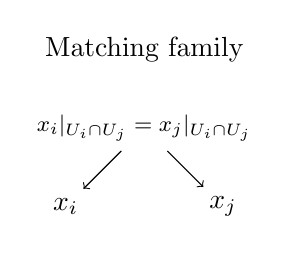
\begin{tikzpicture}[baseline=-1mm]
                \node (title) at (0, 2) {Matching family};
                \node (Uij) at (0, 1) {\footnotesize$x_i|_{U_i\cap U_j} = x_j|_{U_i\cap U_j}$};
                \node (Ui) at (-1, 0) {$x_i$};
                \node (Uj) at (1, 0) {$x_j$};
                \draw[->] (Uij) -- (Ui);
                \draw[->] (Uij) -- (Uj);
            \end{tikzpicture}
            \xrightarrow{\ (2)\ }
            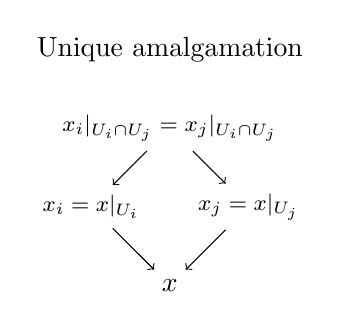
\begin{tikzpicture}[baseline=-1mm]
                \node (title) at (0, 2) {Unique amalgamation};
                \node (Uij) at (0, 1) {\footnotesize$x_i|_{U_i\cap U_j} = x_j|_{U_i\cap U_j}$};
                \node (Ui) at (-1, 0) {\footnotesize$x_i=x|_{U_i}$};
                \node (Uj) at (1, 0) {\footnotesize$x_j=x|_{U_j}$};
                \node (U) at (0, -1) {$x$};
                \draw[->] (Uij) -- (Ui);
                \draw[->] (Uij) -- (Uj);
                \draw[->] (Ui) -- (U);
                \draw[->] (Uj) -- (U);
            \end{tikzpicture}
        \end{gather*}
        The descent condition then states that for every such matching family, there exists a unique element $x$ on $U$, such that the elements of the matching family are restrictions of $x$ as in step $(2)$ of the figure above.

        The classical example would be the assignment of the set of continuous functions to open subsets of a topological space. When two functions, defined on two open sets, coincide on the intersection, there exists a unique continuous function defined on the union, such that it restricts to the given functions.
    \end{example}

    Above, in \cref{topos:coverage}, the notion of a coverage was introduced. It should be clear that every coverage generates a sieve. Furthermore, although coverages are weaker and easier to handle, they are in fact equivalent for the purpose of sheaf theory.
    \begin{property}
        Consider a covering family $C$ and let $S_C$ be the sieve it generates. A presheaf is a sheaf for $C$ if and only if it is a sheaf for $S_C$.
    \end{property}

    \begin{example}[Canonical topology]\index{topology!canonical}
        The canonical topology on a category is the finest Grothendieck topology for which all representable presheaves are sheaves. A \textbf{subcanonical topology} is then defined as a subtopology of the canonical one, i.e.~any Grothendieck topology for which all representable presheaves are sheaves.
    \end{example}
    \begin{example}[Minimal and maximal topologies]
        The minimal Grothendieck topology on a category is the one for which only the maximal sieves are covering sieves. In this topology all presheaves are sheaves. The maximal Grothendieck topology is the one for which all sieves are covering sieves. In this topology only the terminal element of the associated presheaf category is a sheaf.
    \end{example}

    \newdef{Grothendieck topos}{\index{Grothendieck|seealso{topos}}\index{topos!Grothendieck}
        A category equivalent to the category of sheaves on a (small) site. This site is often called the \textbf{site of definition} for the given topos.
    }
    \begin{property}
        Every Grothendieck topos is an elementary topos.
    \end{property}

    \begin{property}
        For every Grothendieck topos, there exists a (standard) site of definition for which the Grothendieck topology is (sub)canonical.
    \end{property}
    \begin{property}
        Let $\mathcal{E}$ be a Grothendieck topos. The canonical topology $J_{\text{can}}$ on $\mathcal{E}$ is the topology for which the covering sieves are jointly epimorphic families. Moreover,
        \begin{gather}
            \mathcal{E}\cong\symbfsf{Sh}(\mathcal{E},J_{\text{can}})\,.
        \end{gather}
    \end{property}

    \begin{construct}[Sheafification]\index{sheafification}
        Given a presheaf $\mathcal{F}$, one can construct a sheaf $\overline{\mathcal{F}}$ along the same lines of \cref{sheaf:colimit_construction}.
    \end{construct}

    \newdef{Global sections functor}{\index{global!sections}\label{topos:global_sections}
        Every Grothendieck topos $\mathcal{E}$ admits a geometric morphism to $\symbfsf{Set}$, where the right adjoint assigns to an object $x$ its set of global elements:
        \begin{gather}
            \Gamma:\mathcal{E}\rightarrow\symbfsf{Set}:x\mapsto\mathcal{E}(1,x)\,.
        \end{gather}
        When $\mathcal{E}$ is the sheaf topos over a topological space, this is exactly the global sections functor (\cref{sheaf:global_sections_functor}). The left adjoint assigns to every set $S$ the copower $S\cdot1\equiv\bigsqcup_{s\in S}1$. When $\mathcal{E}$ is a sheaf topos, this adjoint is exactly the constant sheaf functor. It is sometimes denoted by $\mathrm{LConst}$ (cf.~\cref{sheaf:constant_sheaf}).
    }

    A different approach for defining sheaf topoi is through an embedding of sheaves into presheaves.
    \newdef{Local isomorphism}{\index{local!isomorphism}
        A system of local isomorphisms in $\symbfsf{Psh(C)}$ is a class of morphisms in $\symbfsf{Psh(C)}$ forming a \textit{system of weak equivalences} (see \cref{model:weak_equivalence}) closed under pullbacks along morphisms out of representable presheaves.
    }
    \begin{property}[Local isomorphisms and Grothendieck topologies]
        A system of local isos induces a \textit{system of local epis} in the following way. $f:X\rightarrow Y$ is a local epi if $\im(f)\rightarrow Y$ is a local iso. A Grothendieck topology is defined by declaring a presheaf $F\in\symbfsf{Psh(C)}$ to be a covering sieve at $X\in\ob{C}$ if $F\hookrightarrow\mathcal{Y}X$ is a local epi.
    \end{property}

    \newadef{Sheaf topos}{\index{topos!sheaf}\label{topos:topos_geometric_embedding}
        A category $\symbfsf{Sh(C)}$ equipped with a geometric embedding into $\symbfsf{Psh(C)}$.
        \begin{mdframed}[roundcorner=10pt, linecolor=blue, linewidth=1pt]
            \begin{proof}[Proof of equivalence]
            By \cref{topos:characterization_embedding}, such a category is equivalent to the full subcategory on $S$-local presheaves for some system of local isomorphisms $S$ and, therefore, also to a sheaf topos in the sense of Grothendieck by the property above.
            \end{proof}
        \end{mdframed}
    }

    \begin{remark}[Descent condition]
        This is essentially a restatement of the descent condition (cf.~\ref{topos:local_object_sheaf}). Covering sieves, regarded as subfunctors, are in particular local isomorphisms. Stability of sieves under pullback, together with the co-Yoneda lemma~\ref{cat:ninja_yoneda}, which says that every presheaf is a colimit of representables, generates the full collection of local isomorphisms.
    \end{remark}

    The characterization of geometric embeddings and, hence, of Grothendieck topoi in terms of \textit{localizations} (\cref{topos:characterization_embedding}) is equivalent to a definition in terms of reflections (this is due to \textit{Street}).
    \begin{result}
        There exists a bijection between the Grothendieck topologies on a small category $\symbfsf{C}$ and the equivalence classes of left exact reflective subcategories of $\symbfsf{Psh(C)}$.
    \end{result}

    \newdef{Representable morphism}{\index{representable}
        A natural transformation of presheaves $F\rightarrow G$ is said to be representable if, for every representable presheaf $h_X$ and every morphism $h_X\rightarrow G$, the pullback $h_X\times_GF$ is representable.
    }

    \begin{property}[Diagonals]\label{topos:representable_diagonal}
        The diagonal morphism $\Delta_F:F\rightarrow F\times F$, for $F$ a presheaf on a category with pullbacks, is representable if and only if any of the following two equivalent properties holds:
        \begin{enumerate}
            \item For every two representable presheaves $h_X,h_Y$ and natural transformations $h_X\rightarrow F,h_Y\rightarrow F$, the pullback $h_X\times_Fh_Y$ is representable.
            \item Every natural transformation $h_X\rightarrow F$ from a representable presheaf is representable.
        \end{enumerate}
    \end{property}

\subsection{Topological sheaves}

    See \labelref{chapter:sheaf} for the application of sheaves to topology.

    \begin{property}[Presheaf topos]\label{topos:sheaf_topos}
        Consider the presheaf category
        \begin{gather}
            \symbfsf{Psh}(X):=\symbfsf{Psh\bigl(Open}(X)\bigr)
        \end{gather}
        over a topological space $(X,\tau)$. Unpacking \cref{topos:presheaf_topos} shows that this category is an elementary topos where the subobject classifier is given by
        \begin{gather}
            \Omega(U) = \{V\in\tau\mid V\subseteq U\}\,.
        \end{gather}
    \end{property}

    \begin{construct}[Sheaves and \'etale bundles]\index{bundle}\label{topos:etale_adjunction}
        Let $X$ be a topological space. The functor
        \begin{gather}
            I:\symbfsf{Open}(X)\rightarrow\symbfsf{Top}_{/X}:U\mapsto(U\hookrightarrow X)
        \end{gather}
        induces the following adjunction:
        \begin{gather}
            \symbfsf{Top}_{/X}\adj{E}{\Gamma}\symbfsf{Psh}(X)\,.
        \end{gather}
        The slice category on the left-hand side is the category of (topological) \textit{bundles} (see \labelref{chapter:bundles}) over $X$. Both directions of the adjunction have a clear interpretation. The right adjoint assigns to every bundle its sheaf of local sections and the left adjoint assigns to every presheaf its bundle of germs.

        By restricting to the subcategories on which this adjunction becomes an adjoint equivalence, one obtains the \textbf{\'etale space} and \textbf{sheaf categories} respectively:
        \begin{gather}
            \symbfsf{Et}(X)\cong\symbfsf{Sh}(X)\,.
        \end{gather}
        The category on the right-hand side is the category of sheaves on a topological space $X$. The category on the left is the full subcategory on local homeomorphisms, i.e.~the \'etale spaces (\cref{topology:etale_space}).
    \end{construct}

    \begin{property}[Associated sheaf]
        The inclusion functor $\symbfsf{Sh}(X)\hookrightarrow\symbfsf{Psh}(X)$ admits a left adjoint, the \textbf{sheafification functor}, that assigns to every presheaf its associated sheaf. This functor is given by the composition $\Gamma\circ E$, which is simply \cref{sheaf:etale_construction}.

        The fact that the counit of the adjunction (\cref{topos:etale_adjunction}) restricts to an isomorphism on the full subcategory $\symbfsf{Sh}(X)$ is equivalent to the fact that the sheafification of a sheaf $\Gamma$ is again $\Gamma$.
    \end{property}

    \newdef{Petit and gros topoi\footnotemark}{\index{topos!petit \& gros}\index{topos!spatial}
        \footnotetext{For those that do not master French, `\textit{petit}' and `\textit{gros}' mean small and big, respectively.}
        Consider a topological space $X$ together with its category of opens $\symbfsf{Open}(X)$. The petit topos over $X$ is defined as the sheaf topos $\symbfsf{Sh}(X)\equiv\symbfsf{Sh}\bigl(\symbfsf{Open}(X)\bigr)$. It represents $X$ as a `generalized space'. (By \cref{topos:etale_adjunction}, the objects in a petit topos are the \'etale spaces over the given base space.) Topoi equivalent to such petit topoi are sometimes said to be \textbf{spatial}. However, one can also build a topos whose objects are themselves generalized spaces. To this end, choose a site $S$ of `probes' and call the sheaf topos $\symbfsf{Sh}(S)$ a gros topos. (See \cref{section:smooth_spaces} for more information.)
    }

    \begin{property}[Localic reflection]\index{localic!reflection}
        Mapping a topological space to its sheaf of continuous sections defines a functor $\func{\symbfsf{Sh}}{Top}{Topos}$ by \cref{topos:topological_spaces}. When restricted to the full subcategory of sober spaces (\cref{topology:sober_space}), this functor becomes fully faithful. Generalizing to locales even gives a reflective inclusion (\cref{cat:reflective_inclusion}).

        This property states that no information is lost when regarding (sober) topological spaces as sheaf topoi. This also explains the name `petit topos'.
    \end{property}

    \newdef{Localic topos}{\index{localic!topos}
        Multiple equivalent definitions exist:
        \begin{enumerate}
            \item A topos equivalent to a sheaf topos over a locale (\cref{topology:locale}) equipped with the topology of jointly surjective morphisms.
            \item A topos generated under colimits of subobjects of the terminal object $1$.
            \item A topos $\mathcal{E}$ for which the global sections functor $\Gamma:\mathcal{E}\rightarrow\symbfsf{Set}$ is localic, i.e.~every object in $\mathcal{E}$ is a subquotient of an object in the inverse image $\Gamma^*$
        \end{enumerate}
        Given a geometric morphism to some base topos $\mathcal{S}$, one can define $\mathcal{S}$-localic topoi by generalizing the third point.
    }
    The following property shows that the locale in the first definition has a specific meaning.
    \begin{property}
        By \cref{topos:heyting_algebra}, for every topos the poset $\mathrm{Sub}(1)$ is a locale. Every localic topos $\mathcal{E}$ satisfies $\mathcal{E}\cong\mathrm{Sh}\bigl(\mathrm{Sub}(1)\bigr)$, where $\mathrm{Sub}(1)$ is equipped with the topology of jointly surjective morphisms.
    \end{property}

    The equivalence between localic topoi and locales carries over to the notion of $\mathcal{S}$-localic topoi.
    \begin{property}
        The (2-)category of localic topoi over a base topos $\mathcal{S}$ is equivalent to the (2-)category $\symbfsf{Loc}(\mathcal{S})$ of locales internal to $\mathcal{S}$.
    \end{property}
    \begin{property}\label{topos:slice_locale}
        Given a locale $X$, the category $\symbfsf{Loc}\bigl(\symbfsf{Sh}(X)\bigr)$ is equivalent to the slice category $\symbfsf{Loc}_{/X}$.
    \end{property}

\subsection{Lawvere--Tierney topology}

    This section gives an alternative approach to the construction of sheaf topoi, which is more closely linked to the logical aspect of topos theory.

    \newdef{Lawvere--Tierney topology}{\index{Lawvere--Tierney}
        As noted in \cref{section:internal_logic} on the internal logic of elementary topoi, the subobject classifier $\Omega$ has the structure of an internal Heyting algebra and, in particular, that of a (bounded) meet-semilattice. This internal poset, viewed as an internal category, admits the construction of a closure operator $j:\Omega\rightarrow\Omega$ (\cref{cat:closure_operator}) satisfying the following condition:
        \begin{gather}
            j\circ\land = \land\circ(j\times j)\,.
        \end{gather}
        This condition states (in a nontrivial way) that $j$ is (internally) order-preserving. More concisely, a Lawvere--Tierney topology is internally a left exact modality on $\Omega$.
    }
    \begin{remark}
        The condition satisfied by the unit morphism in the definition of a closure operator can also be reformulated in this context as follows:
        \begin{gather}
            j\circ\texttt{true} = \texttt{true}\,.
        \end{gather}
    \end{remark}

    \begin{example}[Double negation topology]\index{topology!double negation}\label{topos:double_negation}
        As mentioned above, the subobject classifier in an elementary topos has the structure of an internal Heyting algebra and, hence, admits a negation morphism $\lnot:\Omega\rightarrow\Omega$. It can be shown that double negation $\lnot\lnot:\Omega\rightarrow\Omega$ gives a Lawvere--Tierney topology.
    \end{example}
    \begin{property}\index{Booleanization}\index{Boolean!subtopos}\index{dense!subtopos}
        The Booleanization $\mathcal{E}_{\lnot\lnot}\hookrightarrow\mathcal{E}$ of an elementary subtopos is the smallest dense subtopos of $\mathcal{E}$ and the largest Boolean subtopos of $\mathcal{E}$, i.e.~it is the unique subtopos such that:
        \begin{enumerate}
            \item\textbf{Dense}: $\mathcal{E}_{\lnot\lnot}$ contains the initial object $\bot$.
            \item\textbf{Boolean}: $\Omega$ is a Boolean algebra.
        \end{enumerate}
    \end{property}
    
    As noted above, Lawvere--Tierney operators induce, internally, \textit{universal closure operators} on all posets $\mathrm{Sub}(x)$ in the topos. Given an object $x$ and a subobject $u\in\text{Sub}(x)$, one defines the closure $j_\ast(u)\in\text{Sub}(x)$ as the subobject classified by the characteristic morphism $j\circ\chi_u:x\rightarrow\Omega$.
    \newdef{Dense object}{\index{dense}\index{closed}
        Given a Lawvere--Tierney topology $j:\Omega\rightarrow\Omega$, a subobject $u\in\text{Sub}(x)$ is said to be dense (in $x$) if it satisfies $j_\ast(u)\cong x$. An object is said to be \textbf{closed} if $j_\ast(u)\cong u$.
    }

    \begin{example}
        On a presheaf topos, objects are dense exactly if they are covering sieves (\cref{topos:grothendieck_topology}).
    \end{example}

    The following definition allows to generalize sheaves from topoi to finitely complete categories.
    \newadef{Sheaf}{\index{sheaf}\index{separated}
        Given a Lawvere--Tierney topology $j:\Omega\rightarrow\Omega$ on a topos $\mathcal{E}$, one calls an object $s\in\ob{\mathcal{E}}$ a $j$-sheaf if it is local with respect to all dense morphisms (\cref{cat:local_object}), i.e.~for all dense morphisms $u\hookrightarrow x$ the induced map \[\mathcal{E}(x,s)\rightarrow\mathcal{E}(u,s)\] is a bijection. If this map is only a monomorphism, the object is said to be \textbf{$j$-separated}.
    }

    \begin{property}\index{sheafification}
        Lawvere--Tierney topologies on $\mathcal{E}$ are in correspondence with subtopoi of $\mathcal{E}$, given by the sheaves relative to the chosen topology. As before, the left adjoint to the embedding is the sheafification functor.
    \end{property}

    In the case of (pre)sheaf topoi, Lawvere--Tierney topologies recover Grothendieck topologies.
    \begin{result}
        For the presheaf topos on a small category $\symbfsf{C}$, the Grothendieck topologies on $\symbfsf{C}$ are equivalent to Lawvere--Tierney topologies on $\symbfsf{Psh(C)}$.
        \begin{mdframed}[roundcorner=10pt, linecolor=blue, linewidth=1pt]
            \begin{proof}[Sketch of proof]
                Since a Grothendieck topology assigns to every object a collection of sieves, \cref{topos:presheaf_topos} implies that $J(x)\subseteq\Omega_{\symbfsf{Psh}}(x)$ for all $x\in\ob{C}$. By the base change condition of Grothendieck topologies, this relation is natural in $x$ and, hence, $J$ is a subobject of $\Omega_{\symbfsf{Psh}}$. One thus finds a characteristic morphism $j:\Omega_{\symbfsf{Psh}}\rightarrow\Omega_{\symbfsf{Psh}}$ that can be proven (by the other conditions of Grothendieck topologies) to define a Lawvere--Tierney topology on $\symbfsf{Psh(C)}$. Conversely, a Lawvere--Tierney topology is a morphism $j:\Omega\rightarrow\Omega$ and, hence, determines a unique subobject of $\Omega_{\symbfsf{Psh}}$, i.e.~a unique collection of sieves for every object $x\in\ob{C}$. From the conditions of Lawvere--Tierney topologies, one can then prove that this collection satisfies the conditions of a Grothendieck topology.
            \end{proof}
        \end{mdframed}
    \end{result}

\subsection{Diaconescu's theorem}\label{section:diaconescu}\index{Diaconescu}

    The following concept weakens the notion of left exact functors to categories where not all (finite) limits exist.
    \newdef{Flat functor}{\index{flat!functor}\label{topos:flat_functor}
        A functor $\func{F}{C}{Set}$ is said to be flat if the opposite of the category of elements $\mathrm{El}(F)^{\text{op}}$ (\cref{cat:category_of_elements}) is filtered (\cref{cat:filtered}). The category of flat functors on $\symbfsf{C}$ is denoted by $\symbfsf{Flat}(\symbfsf{C},\symbfsf{Set})$.

        A general functor $\func{F}{C}{D}$ is said to be \textbf{(representably) flat} if, for every object $d\in\ob{D}$, the opposite comma category $(d/F)^{\text{op}}$, which is equivalently the opposite category of elements $\mathrm{El}\bigl(\symbfsf{D}(d,-)\circ F\bigr)^{\text{op}}$, is filtered.
    }

    The definitions above can be stated more explicitly as follows (cf.~\cref{cat:finitely_complete_alternative}). The functor $\func{F}{C}{D}$ is representably flat if for every $d\in\ob{D}$:
    \begin{enumerate}
        \item There is at least one object $c\in\ob{C}$ and a morphism $f:d\rightarrow Fc$. Hence, at least one inhabited set in the image of $F$.
        \item For every two objects $c,c'\in\ob{C}$ and every two morphisms $f\in\symbfsf{D}(d,Fc)$ and $g\in\symbfsf{D}(d,Fc')$, there exists an object $x\in\ob{C}$ and morphisms $i\in\symbfsf{C}(x,c)$, $j\in\symbfsf{C}(x,c')$ and $h\in\symbfsf{D}(d,Fx)$ such that $Fi\circ h=f$ and $Fj\circ h=g$.
        \item For every two parallel morphisms $f,g\in\symbfsf{C}(c,c')$ and morphism $h\in\symbfsf{D}(d,Fc)$ such that $Ff\circ h=Fg\circ h$, there exists a morphism $i\in\symbfsf{C}(x,c)$ and a morphism $j\in\symbfsf{D}(d,Fx)$ such that $f\circ i=g\circ i$ and $Fi\circ j=h$.
    \end{enumerate}

    \begin{remark}
        Note that flatness and representable flatness are only equivalent for $\symbfsf{Set}$-valued functors when the domain $\symbfsf{C}$ is finitely complete.
    \end{remark}

    \begin{property}\index{Yoneda!extension}
        Consider the \textbf{Yoneda extension} that maps a functor $F\in\funccat{C}{Set}$ to a functor $\widetilde{F}:\cfunccat{C}{Set}\rightarrow\symbfsf{Set}$ through left Kan extension along the Yoneda embedding. $F$ is flat if and only if $\widetilde{F}$ is left exact.\footnote{By \cref{cat:kan_extension_alternative}, Kan extensions admit an expression is terms of adjoints. In this setting, the right adjoint has the form of a Hom-functor and, accordingly, the Yoneda extension is sometimes written as a tensor product $-\otimes_{\symbfsf{C}}F$. The terminology `flat' is then in analogy with \cref{homalg:flat_module}. This essentially coincides with the tensor product of functors \cref{cat:copower_product}.}
    \end{property}
    \begin{property}\label{topos:flat_or_ind}
        A functor $\func{F}{C}{Set}$ is flat if and only if it is the filtered colimit of representable functors or, equivalently, if $F$-weighted filtered colimits commute with finite limits. Note that, by \cref{cat:pro_object_uproperty}, this means that
        \begin{gather}
            \symbfsf{Flat(\op{C},Set)}\cong\symbfsf{Ind(C)}\,.
        \end{gather}
    \end{property}

    The previous property implies the following statement, which is the $\symbfsf{Set}$-valued version of \textit{Diaconescu's theorem}, which will be covered in its internal version below.
    \begin{theorem}[Diaconescu: Set version]
        A functor $\func{F}{C}{Set}$ is flat if and only if the induced adjunction $\symbfsf{Set}\leftrightarrows\cfunccat{C}{Set}$ is a geometric morphism or, alternatively, if flat functors are equivalent to global points of the presheaf topos $\cfunccat{C}{Set}$.
    \end{theorem}

    \newdef{Morphism of sites}{\index{morphism!of sites}
        A representably flat functor preserving covers.
    }

    Now, for $\mathcal{E}$ a cocomplete topos, a functor $\func{F}{C}{\mathcal{E}}$ is said to be \textbf{(internally) flat} if it representably flat with respect to the internal logic of $\mathcal{E}$ or, equivalently, if the Yoneda extension $\mathrm{Lan}_{\mathcal{Y}}F$ is left exact.
    \begin{property}\index{flat!functor}
        A functor $\func{F}{C}{\mathcal{E}}$, with $\mathcal{E}$ a cocomplete topllos, is flat if and only if:
        \begin{itemize}
            \item The family of terminal morphisms in $\symbfsf{C}$ is jointly epimorphic.
            \item For all $c,d\in\ob{C}$, the family of morphisms into $Ac\times Ad$ induced by spans $c\leftarrow b\rightarrow d$ is jointly epimorphic.
            \item For any two parallel morphisms $f,g$ in $\symbfsf{C}$, the family of factorizations of morphisms through their equalizer is jointly epimorphic.
        \end{itemize}
        These conditions are equivalent to the following ones:
        \begin{itemize}
            \item For every object $x\in\mathcal{E}$, there exists a jointly epimorphic family $\{x_i\rightarrow x\}_{i\in I}$ and and a family $\{x_i\rightarrow F(c_i)\mid c_i\in\ob{C}\}_{i\in I}$.
            \item For all $c,d\in\ob{C}$ and generalized elements $\lambda:x\rightarrow Fc\times Fd$, there exists an epimorphic family $\{\lambda_i:x_i\rightarrow x\}_{i\in I}$ and a family of spans $\{c\xleftarrow{f}b_i\xrightarrow{g}d\}_{i\in I}$ equipped with a family of generalized elements $\{\kappa_i:x_i\rightarrow Fb_i\}_{i\in I}$ such that
            \begin{gather}
                (Ff,Fg)\circ\kappa_i = \lambda\circ\lambda_i\,.
            \end{gather}
            \item For any two parallel morphisms $f,g:c\rightarrow d$ in $\symbfsf{C}$ and any generalized element $\lambda:x\rightarrow Fc$ such that $Ff\circ\lambda=Fg\circ\lambda$, there exists an epimorphic family $\{\lambda_i:x_i\rightarrow x\}_{i\in I}$ and families of morphisms $\{f_i:c_i\rightarrow c\}$ and $\{\kappa_i:x_i\rightarrow Fc_i\}$ such that
            \begin{gather}
                \begin{aligned}
                    f\circ f_i &= g\circ f_i\\
                    Ff_i\circ\kappa_i &= \lambda\circ\lambda_i
                \end{aligned}
            \end{gather}
            for all $i\in I$.
        \end{itemize}
    \end{property}

    \begin{theorem}[Diaconescu: Topos version]
        Consider a cocomplete topoi $\mathcal{E}$ and a (small) category $\symbfsf{C}$. There exists an equivalence
        \begin{gather}
            \symbfsf{Topos}\bigl(\mathcal{E},[\symbfsf{C}^{\mathrm{op}},\symbfsf{Set}]\bigr)\leftrightarrows\symbfsf{Flat}(\symbfsf{C},\mathcal{E})\,,
        \end{gather}
        where
        \begin{itemize}
            \item flat functors are sent to geometric morphisms whose inverse image part is given by left Kan extension along the Yoneda embedding and direct image part is given by:
            \begin{gather}
                F\mapsto\bigl(x\mapsto\mathcal{E}(F-, x)\bigr)\,,
            \end{gather}
            and
            \item geometric morphisms are sent to the precomposition of the inverse image part with the Yoneda embedding.
        \end{itemize}
    \end{theorem}

    To pass to the internal logic of topoi, \cref{cat:filtered} needs to be generalized to internal category theory (\cref{section:internal_category_theory}).
    \newdef{Internally filtered category}{\index{category!filtered}
        An internal category $\symbfsf{C}\in\symbfsf{Cat}(\mathcal{E})$ satisfying:\footnote{Some sources require all these morphisms to be regular epis.}
        \begin{enumerate}
            \item The terminal morphism $C_0\twoheadrightarrow1$ is an epi.
            \item For any two generalized elements $\lambda_1,\lambda_2:U\rightarrow C_0$, there is an epi $\theta:V\twoheadrightarrow U$ and corresponding $V$-elements $\gamma_1,\gamma_2:V\rightarrow C_0$ such that
            \begin{gather}
                \begin{aligned}
                    d_1\circ\gamma_1 &= d_1\circ\gamma_2\\
                    d_0\circ\gamma_i &= \lambda_i\circ\theta
                \end{aligned}
            \end{gather}
            for $i=1,2$.
            \item For any two parallel generalized elements $\gamma_1,\gamma_2:U\rightarrow C_1$ such that $d_0\circ\gamma_1=d_0\circ\gamma_2$, there exists an epi $\theta:V\twoheadrightarrow U$ and a $V$-element $\kappa:V\rightarrow C_1$ such that
            \begin{gather}
                \begin{aligned}
                    d_1\circ\kappa &= d_0\circ\lambda_1\circ\theta = d_0\circ\lambda_2\circ\theta\\
                    c(\kappa,\lambda_1\circ\theta) &= c(\kappa,\lambda_2\circ\theta)\,.
                \end{aligned}
            \end{gather}
        \end{enumerate}
    }
% \chapter{\difficult{Model theory}}\label{chapter:model_theory}

    General references for this chapter are~\citet{hovey_model_2007,riehl_homotopical_2019}. For more on monoidal model categories, see~\citet{riehl_monoidal_2013}. A good reference for the section on simplicial spaces and, in particular, the theory of Segal spaces is~\citet{rezk_model_2001}. For more on Reedy model structures, see~\citet{riehl_theory_2013}. A gentle introduction to the theory of homotopy (co)limits can be found in~\citet{riehl_homotopy_2011,lambrechts_gentle_2013}. The content and language of \cref{chapter:hom_alg} will be used throughout this chapter.

    \minitoc

\section{Simplicial sets}

    \newdef{Simplex category}{\index{simplex!category}\label{model:simplex_category}
        The simplex category $\simplex$ has as objects the posets of the form $[n]:=\{0<\cdots<n\}$ and as morphisms the order-preserving maps.
    }
    \newdef{Simplicial set}{\index{simplicial!set}\label{model:simplicial set}
        The category $\symbfsf{sSet}$ of simplicial sets is defined as the presheaf category $\symbfsf{Psh}(\simplex)$. For all $n\in\mathbb{N}$, the set of \textbf{$n$-simplices in} $X$ is defined as the set $X_n:=X([n])$.
    }
    \newdef{Simplicial object}{\index{simplicial!object}\label{model:simplicial_object}
        By internalizing the notion of a simplicial set, one obtains the definition of a simplicial object, i.e.~a simplicial object in a category $\symbfsf{C}$ is a $\symbfsf{C}$-valued presheaf on $\simplex$.
    }
    \begin{remark}
        Note that the notion of \textbf{simplicial category} can mean two distinct things. In general, it will mean a category enriched in $\symbfsf{sSet}$. However, following the previous definition, it can also mean a simplicial object in the (2-)category $\symbfsf{Cat}$. It can be shown that all simplicially enriched categories are a specific kind of degenerate simplicial object in $\symbfsf{Cat}$, where the face and degeneracy maps are identity-on-objects.
    \end{remark}

    \newdef{Standard simplex}{\index{simplex}\label{model:standard_simplex}
        For every $n\in\mathbb{N}$, the standard $n$-simplex $\Delta[n]$ is defined as the Yoneda embedding $\simplex(-,[n])$. One can also define a functor $\func{\Delta_{\mathrm{top}}}{\simplex}{Top}$ that maps $[n]$ to the standard topological $n$-simplex $\Delta^n$ (\cref{topology:standard_simplex}).
    }
    \begin{property}
        By the Yoneda lemma, there exists a natural bijection between the set of $n$-simplices of a simplicial set $X$ and the set of maps $\Delta[n]\rightarrow X$.
    \end{property}

    \begin{property}[Face and degeneracy maps]\index{face!map}\index{degeneracy map}
        All morphisms in the simplex category $\simplex$ are generated by morphisms of the following two types:
        \begin{itemize}
            \item For every $n$ and $i<n$, the unique map $\delta_{n,i}:[n-1]\rightarrow[n]$ that misses the $i^{\text{th}}$ element.
            \item For every $n$ and $i\leq n$, the unique map $\sigma_{n,i}:[n+1]\rightarrow[n]$ that duplicates the $i^{\text{th}}$ element.
        \end{itemize}
        Under the action of a presheaf, this gives the \textbf{face} and \textbf{degeneracy} maps $d_{n,i}$ and $s_{n,i}$. (If the index $n$ is clear, it is often omitted.)

        These morphisms satisfy the fundamental \textbf{simplicial identities}:
        \begin{itemize}
            \item $d_i\circ d_j = d_{j-1}\circ d_i$ for $i<j$,
            \item $d_i\circ s_j = s_{j-1}\circ d_i$ for $i<j$,
            \item $d_i\circ s_j = \mathbbm{1}$ for $i=j$ or $i=j+1$,
            \item $d_i\circ s_j = s_j\circ d_{i-1}$ for $i>j+1$, and
            \item $s_i\circ s_j = s_{j+1}\circ s_i$ for $i\leq j$.
        \end{itemize}
    \end{property}

    \newdef{Connected components}{\index{connected!component}
        Consider a simplicial set $X$. Its set of connected components $\pi_0(X)$ is defined as the quotient of $X_0$ under the relation
        \begin{gather}
            X_1\underset{d_1}{\overset{d_0}{\rightrightarrows}}X_0\times X_0\,.
        \end{gather}
        This defines a fucntor $\func{\pi_0}{sSet}{Set}$. By base change \ref{cat:change_of_base}, this also induces a functor on simplicial categories.
    }

\subsection{Constructions}

    \begin{construct}[Nerve and realization]\label{model:nerve_and_realization}
        Consider a general functor $\func{F}{S}{C}$ into a cocomplete category ($\symbfsf{S}$ will often be a category of geometric shapes such as the simplex category $\simplex$ or the \textit{cube category} $\mbox{\mancube}$). Every such functor induces an adjunction
        \begin{gather}
            \symbfsf{C}\adj{|-|}{N}\symbfsf{Psh}(\symbfsf{S})\,.
        \end{gather}
        The \textbf{realization functor} $|-|$ is defined as the left Kan extension $\mathrm{Lan}_{\mathcal{Y}}F$. The \textbf{nerve functor} $\func{N}{C}{Psh(S)}$ is defined as $Nx:=\symbfsf{C}(F-,x)=\mathcal{Y}x\circ F$.

        This definition can easily be generalized to the enriched setting. Furthermore, if one assumes that $\symbfsf{C}$ is copowered over $\mathcal{V}$, the realization functor can be expressed as a coend:
        \begin{gather}
            |X| = \int^{s\in\symbfsf{S}}Xs\cdot Fs\,.
        \end{gather}
    \end{construct}

    \begin{example}[Nerve of a category]\index{nerve}\label{model:nerve}
        To every small category $\symbfsf{C}$, one can associate a simplicial set $N\symbfsf{C}$ in the following way. The set $N\symbfsf{C}_0$ is given by the set of objects in $\symbfsf{C}$ and the set $N\symbfsf{C}_1$ is given by the set of morphisms in $\symbfsf{C}$. Now, for every two composable morphisms $f,g$, one obtains a canonical commuting triangle by composition. Let $N\symbfsf{C}_2$ be the set of all these triangles. The higher simplices are defined analogously. Face maps act by composing morphisms or by dropping the exterior morphisms in a composable string. Degeneracy maps act by inserting an identity morphism.

        Equivalently, one can define the \textbf{simplicial nerve functor} in the following way. Every poset $[n]$ admits a canonical category structure for which the order-preserving maps give rise to the associated functors. By the above construction, this inclusion $\simplex\hookrightarrow\symbfsf{Cat}$ induces a nerve functor
        \begin{gather}
            N:\symbfsf{Cat}\rightarrow\symbfsf{sSet}:\symbfsf{C}\mapsto\symbfsf{Cat}(-,\symbfsf{C})\,.
        \end{gather}
        This way, one obtains $N\symbfsf{C}_k=\symbfsf{Cat}([k], \symbfsf{C})$. This object is, by definition, equivalent to the collection of all strings of $k$ composable morphisms in $\symbfsf{C}$. It can be shown that the simplicial nerve functor is fully faithful.
    \end{example}

    \begin{example}[Geometric realization]\index{geometric!realization}\label{model:geometric_realization}
        Consider a simplicial set $X$. From this object, one can construct a topological space as follows. First, take a point for every element in $X_0$. Then, glue 1-simplices between these points using the face maps. The higher (nondegenerate) simplices are attached analogously.

        More abstractly, the geometric realization functor $\func{|\cdot|}{sSet}{Top}$ is defined as a (left) Kan extension:
        \begin{gather}
            |\cdot| := \mathrm{Lan}_{\mathcal{Y}}\Delta_\mathrm{top}\,.
        \end{gather}
        An application of the Yoneda lemma shows that the geometric realization can be expressed as a functor tensor product (\cref{cat:functor_tensor_product}):
        \begin{gather}
            |X| = X\otimes_{\simplex}\Delta_\mathrm{top}=\int^{n\in\simplex}\Delta^n\cdot X_n\,.
        \end{gather}
        This formula can easily be generalized to the category of simplicial topological spaces ($\symbfsf{sSet}$ is a full subcategory obtained by endowing every set with the discrete topology). In $\symbfsf{Top}$, the coend can be expressed as the quotient space
        \begin{gather}
            |X| := \bigsqcup_{n\in\mathbb{N}}X_n\times\Delta^n/\sim\,,
        \end{gather}
        where the equivalence relation identifies the points $(x,f_*y)$ and $(f^*x,y)$ for all morphisms $f\in\mathrm{hom}(\simplex)$. The morphisms $f^*,f_*$ are the ones induced by $X$ and $\Delta_\mathrm{top}:\simplex\hookrightarrow\symbfsf{Top}$. As an immediate example one obtains
        \begin{gather}
            |\Delta[n]| = \Delta^n\,,
        \end{gather}
        which shows that $\Delta[n]$ really deserves to be called the standard $n$-simplex.
    \end{example}
    \begin{remark}\index{geometric!realization}\label{model:geometric_realization_categories}
        Note that the composition of the geometric realization and (simplicial) nerve functors $\func{|N\cdot|}{Cat}{Top}$ is also often called the \textbf{geometric realization} (of categories).
    \end{remark}

    \begin{example}[Singular set]\index{set!singular}\label{model:singular_set}
        Given a topological space $X$, one can define a simplicial set $\mathrm{Sing}(X)$. Its components are defined as the set of morphisms from the standard (topological) $n$-simplex to $X$:
        \begin{gather}
            \mathrm{Sing}(X)_n := \symbfsf{Top}(\Delta^n,X)\,.
        \end{gather}
        This is the object of relevance in the definition of singular (co)homology as given in \cref{section:singular_homology}.
    \end{example}

    \begin{property}[Classifying space]\index{bar construction}\index{classifying!space}\label{model:classifying_space}
        For a (discrete) group $G$, one can construct two important objects: the delooping $\symbfsf{B}G$ (\cref{cat:group_delooping}) and the \textit{classifying space} $BG$ (see \cref{bundle:classifying_space}). As their notations imply, there exists a relation between these space. By taking the geometric realization of $\symbfsf{B}G$, one obtains $BG$. In fact, this method can be applied to any monoid $A$ to obtain the so-called (two-sided) \textbf{bar construction}.
    \end{property}

    \begin{construct}[Join]\index{join}
        Consider two simplicial sets $X,Y$. An explicit construction of the join $X\star Y$ is as follows:
        \begin{gather}
            (X\star Y)_n := X_n\sqcup Y_n\sqcup\bigsqcup_{i+j=n-1}X_i\times Y_j\,.
        \end{gather}
        The boundary maps on the first two components are those of $X$ and $Y$. On the third component it acts by
        \begin{gather}
            \dr_i(x,y) :=
            \begin{cases}
                (\dr_ix,y)&\cif i\leq j,j\neq0\,,\\
                (x,\dr_{i-j-1}y)&\cif i>j,k\neq0\,,
            \end{cases}
        \end{gather}
        where $x\in X_j$ and $y\in Y_k$. For $j=0$ and $k=0$, the projections are used.
    \end{construct}

\subsection{Homological algebra}

    In this section, simplicial sets are related to homological algebra (\cref{chapter:hom_alg}). A basic introduction is~\citet{master_why_2020}.

    \begin{construct}[Alternating face map complex]\index{normalized!complex}
        From a simplicial Abelian group $A$, one can construct a connective chain complex as follows. For every $n\in\mathbb{N}$, define
        \begin{gather}
            (CA)_n := A_n\,.
        \end{gather}
        The boundary maps $\delta_n$ are defined as the alternating sum of the face maps:
        \begin{gather}
            \delta_n := \sum_{i=1}^n(-1)^idr_i\,.
        \end{gather}
        Every group $A_{n+1}$ contains a subgroup $D(A_n)$ generated by the degeneracy maps:
        \begin{gather}
            D(A_n) := \left\langle\bigcup_{i=1}^ns_i(A_n)\right\rangle\,.
        \end{gather}
        If these degenerate simplices are quotiented out, the \textbf{normalized complex} is obtained.
    \end{construct}
    This construction can be generalized to any simplicial group:
    \begin{construct}[Moore complex]\index{Moore!complex}
        Let $G$ be a simplicial group. For every $n\in\mathbb{N}$, define
        \begin{gather}
            (NG)_n := \bigcap_{i=1}^n\ker(\dr^n_i)\,.
        \end{gather}
        The differential $\partial_n$ is given by the zeroth face map $d^n_0$.
    \end{construct}
    \begin{property}[Equivalence]
        For simplicial Abelian groups, the Moore complex and normalized complex are isomorphic. Moreover, the inclusion of the normalized complex into the alternating face map complex is a quasi-isomorphism.
    \end{property}

    \begin{theorem}[Dold--Kan correspondence]\index{Dold--Kan correspondence}\label{model:dold_kan}
        The functor that maps simplicial Abelian groups to normalized chain complexes gives an equivalence of categories $\symbfsf{sAb}\cong\symbfsf{Ch}^+(\symbfsf{Ab})$.
    \end{theorem}

\section{Localization}\label{section:localization}

    \newdef{Category with weak equivalences}{\index{weak!equivalence}\label{model:weak_equivalence}
        A category $\symbfsf{C}$ with a subcategory $\symbfsf{W}$ such that:
        \begin{enumerate}
            \item $\symbfsf{W}$ contains all isomorphisms in $\symbfsf{C}$ (in particular, $\symbfsf{W}$ is wide).
            \item $\symbfsf{W}$ satisfies the `2-out-of-3 property': If any two of $\{f,g,f\circ g\}$ are in $\mathrm{hom}(\symbfsf{W})$, so is the third.
        \end{enumerate}
    }

    \newdef{Weak factorization system}{\index{factorization!weak}\label{model:wfs}
        Consider a category $\symbfsf{C}$. A pair $(L,R)$ of classes of morphisms in $\symbfsf{C}$ is called a weak factorization system (WFS) if it satisfies the following properties:
        \begin{enumerate}
            \item Every morphism in $\symbfsf{C}$ factorizes as $g\circ f$ where $f\in L$ and $g\in R$.
            \item $L$ consists of exactly those morphisms in $\symbfsf{C}$ that have the left lifting property (\cref{cat:lifting_property}) with respect to morphisms in $R$.
            \item $R$ consists of exactly those morphisms in $\symbfsf{C}$ that have the right lifting property with respect to morphisms in $L$.
        \end{enumerate}
    }
    \begin{remark*}
        The original definition by \textit{Quillen} only required that $L$ and $R$ satisfied the lifting properties with respect to each other, not that they were closed under this condition. This was enforced by a further condition that both $L$ and $R$ are closed under retracts in the arrow categories. It can be proven that this is equivalent to the definition above.
    \end{remark*}

    \newdef{Homotopical category}{\index{category!homotopical}
        A category $\symbfsf{C}$ equipped with a subcategory $\symbfsf{W}$ such that:
        \begin{enumerate}
            \item $\symbfsf{W}$ contains all identity morphisms in $\symbfsf{C}$
            (in particular, $\symbfsf{W}$ is wide).
            \item $\symbfsf{W}$ satisfies the `2-out-of-6 property': If $f\circ g$ and $g\circ f$ are in $\mathrm{hom}(\symbfsf{W})$, so are $f,g,h$ and $f\circ g\circ h$.
        \end{enumerate}
        It is not hard to see that every homotopical category is, in particular, a category with weak equivalences.
    }
    \newdef{Homotopical functor}{\index{functor!homotopical}
        A functor (between homotopical categories) that preserves weak equivalences.
    }

    \newdef{Gabriel--Zisman localization}{\index{localization!Gabriel--Zisman}\label{model:localization}
        Consider a category $\symbfsf{C}$ with a collection of morphisms $M\subset\mathrm{hom}(\symbfsf{C})$. The localization of $\symbfsf{C}$ with respect to $M$ is constructed by adding for each morphism $f\in M$ a formal inverse to $\mathrm{hom}(\textbf{C})$.

        More specifically, the localization consists of a category $\symbfsf{C}[M^{-1}]$ and a functor $F_M:\symbfsf{C}\rightarrow\symbfsf{C}[M^{-1}]$ inverting $M$, i.e.~mapping all morphisms in $M$ to isomorphisms, that is universal with respect to this property.

        When $\symbfsf{C}$ has finite products, the localization $C[x^{-1}]$ at an object $x\in\ob{C}$ is given by the localization at the projections $M_x:=\bigl\{y\times x\rightarrow y\mid y\in\ob{C}\bigr\}$.
    }

    \newdef{Homotopy category I}{\index{homotopy!category}
        When $\symbfsf{C}$ is a category with weak equivalences $W$, the localization $\symbfsf{C}[W^{-1}]$ is called the homotopy category $\symbfsf{Ho(C)}$. In this context, the localization functor $\symbfsf{C}\rightarrow\symbfsf{Ho(C)}$ is sometimes denoted by $\gamma_{\symbfsf{C}}$.
    }
    \begin{remark}[Size issues]
        When $\symbfsf{C}$ is small, so is its localization. However, even in the case where $\symbfsf{C}$ is locally small, its localization might be large.
    \end{remark}

    \newprop{Reflective localization}{\index{reflective!localization}\label{model:reflective_localization}
        Consider an adjunction $\func{F\dashv G}{C}{D}$. The right adjoint is fully faithful, i.e.~determines a reflective subcategory (\cref{cat:reflective_inclusion}), if and only if $F$ realizes $\symbfsf{D}$ as a localization of $\symbfsf{C}$. The essential image of $G$ consists exactly of the local objects in $C$.
    }

    \newdef{Derived functor}{\index{derived!functor}\label{model:derived_functor}
        Consider a homotopical functor $\func{F}{C}{D}$ and consider the composition $\gamma:=\gamma_{\symbfsf{D}}\circ F$ with the localization functor $\func{\gamma_{\symbfsf{D}}}{D}{Ho(D)}$. The derived functor $\func{\symbfsf{Ho}(F)}{Ho(C)}{Ho(D)}$ is obtained by applying the universal property of $\symbfsf{Ho(C)}$ to $\gamma$.

        This definition can be rephrased in terms of Kan extensions. Consider a homotopical functor $\func{F}{C}{D}$. The left and right derived functors are defined as the following Kan extensions:
        \begin{gather}
            \begin{aligned}
                LF &:= \mathrm{Ran}_{\gamma_{\symbfsf{C}}}(\gamma_{\symbfsf{D}}\circ F)\,,\\
                RF &:= \mathrm{Lan}_{\gamma_{\symbfsf{C}}}(\gamma_{\symbfsf{D}}\circ F)\,.
            \end{aligned}
        \end{gather}
        In fact, one can drop the assumption that $\symbfsf{D}$ has weak equivalences (here, $F$ should map weak equivalences to isomorphisms). In this case, one simply has to replace $\gamma_{\symbfsf{D}}\circ F$ by $F$ in the above formulas.
    }

    \begin{example}[Derived category]\index{derived!category}
        Consider an Abelian category $\symbfsf{C}$ together with its category of chain complexes $\symbfsf{Ch(C)}$. The derived category $\mathcal{D}(\symbfsf{C})$ is defined as the localization of $\symbfsf{Ch(C)}$ at the quasi-isomorphisms.
    \end{example}
    \begin{remark}
        In this case, it can be shown that one can first restrict to the naive homotopy category $\symbfsf{K(C)}$, consisting of chain complexes and chain maps up to chain homotopy, and then localize at the collection of quasi-isomorphisms.
    \end{remark}

\section{Model categories}\label{section:model_categories}
\subsection{Model structures}

    \newdef{Model structure}{\index{fibration}\index{acyclic!morphism}
        Let $\symbfsf{C}$ be a category. A (\textbf{Quillen}-)model structure on $\symbfsf{C}$ consists of three classes of morphisms:
        \begin{itemize}
            \item\textbf{weak equivalences} $W$,
            \item\textbf{fibrations} $\mathrm{Fib}$, and
            \item\textbf{cofibrations} $\mathrm{Cof}$,
        \end{itemize}
        that satisfy the following two conditions:
        \begin{enumerate}
            \item $W$ turns $\symbfsf{C}$ into a category with weak equivalences (\cref{model:weak_equivalence}).
            \item $(\mathrm{Cof},\mathrm{Fib}\cap W)$ and $(\mathrm{Cof}\cap W,\mathrm{Fib})$ are weak factorization systems (\cref{model:wfs}).
        \end{enumerate}
        The morphisms in $\mathrm{Fib}\cap W$ and $\mathrm{Cof}\cap W$ are said to be \textbf{acyclic} or \textbf{trivial}.
    }
    \sremark{That $W$ contains all isomorphisms follows from the property that any class of morphisms satisfying a lifting property contains all isomorphisms.}

    \newdef{Model category}{\index{model!category}\index{category!model|see{model category}}
        A bicomplete category equipped with a model structure.\footnote{\textit{Quillen}'s original definition only required the existence of finite limits and finite colimits.}
    }
    \newdef{Proper model category}{\index{proper!model category}
        A model category is said to be left proper (resp.~right proper) if weak equivalences are preserved by pushouts along cofibrations (resp.~pullbacks along fibrations).
    }

    \newdef{Fibrant object}{\index{fibrant object}
        An object in a model category for which the terminal morphism is a fibration. Dually, an object in a model category is said to be cofibrant if the initial morphism is a cofibration.
    }

    \begin{example}[Model structure on functor categories]\label{model:model_functor_category}
        In some cases, the functor category $\funccat{C}{D}$, for $\symbfsf{C}$ small and $\symbfsf{D}$ a model category, admits two canonical model structures:
        \begin{itemize}
            \item\textbf{Injective model structure}: The weak equivalences are the natural transformations that are objectwise weak equivalences and the cofibrations are the natural transformations that are objectwise cofibrations.
            \item\textbf{Projective model structure}: The weak equivalences are the natural transformations that are objectwise weak equivalences and the fibrations are the natural transformations that are objectwise fibrations.
        \end{itemize}
    \end{example}

    \begin{property}[Resolution]\index{resolution}
        In a model category, the bicompleteness property implies that the initial and terminal object always exist. The weak factorization property then implies that, for every object $x$, one can find a weakly equivalent fibrant replacement $x^\mathrm{f}$ and a weakly equivalent cofibrant replacement $x^\mathrm{cf}$ by suitably factorizing the initial and terminal morphisms. These replacements are sometimes called \textbf{resolutions} or \textbf{approximations}.

        If the weak factorization system is functorial (\cref{cat:functorial_factorization}), (co)fibrant replacement defines an endofunctor that is weakly equivalent to the identity functor.
    \end{property}

    \newdef{Quillen adjunction}{\index{Quillen!adjunction}
        Let $\symbfsf{C,D}$ be two model categories. An adjunction \[\symbfsf{D}\adj{F}{G}\symbfsf{C}\] is called a \textbf{Quillen adjunction} if the left adjoint preserves cofibrations and acyclic cofibrations. The model category axioms imply that this is equivalent to requiring that the right adjoint preserves fibrations and acyclic fibrations. The adjoint functors are called (left and right) \textbf{Quillen functors}.

        If $F\dashv G$ is a Quillen adjunction, such that, for all cofibrant objects $x$ and fibrant objects $y$, the morphism $Fx\rightarrow y$ is a weak equivalence if and only if the adjunct $x\rightarrow Gy$ is a weak equivalence, then $F\dashv G$ is called a \textbf{Quillen equivalence}.
    }

    Quillen equivalences can also be characterized at the homotopical level.
    \begin{property}
        A Quillen adjunction $F\dashv G$ is a Quillen equivalence if and only if the left derived functor $LF$ (or right derived functor $RG$) is an equivalence.
    \end{property}
    \begin{property}[Derived adjunction]
        If $F\dashv G$ is a Quillen adjunction, the derived functors $(LF,RG)$ also form an adjunction.
    \end{property}

    \begin{property}[Doubly categorical interpretation]
        The map that sends a model category to its homotopy category and a Quillen functor to its derived functor is a \textit{double pseudofunctor}. Amongst other things, this implies that the composition of derived functors is naturally weakly equivalent to the derived functor of the composition.
    \end{property}

    \begin{example}[Topological spaces]
        A first example of model categories is the category $\symbfsf{Top}$ of topological spaces (\cref{chapter:topology} and \cref{chapter:algtop}). This category can be endowed with a model structure by taking the weak equivalences to be the weak homotopy equivalences (\cref{topology:weak_equivalence}) and by taking the fibrations to be the Serre fibrations (\cref{topology:fibration}).
    \end{example}
    \begin{example}[Simplicial sets]\index{Quillen!model structure}\label{model:sset_model_structure}
        As a second example, consider the category $\symbfsf{sSet}$. This category can be turned into a model category by taking the weak equivalences to be the morphisms that induce weak homotopy equivalences between geometric realizations and by taking the fibrations to be Kan fibrations. With this structure, the fibrant objects are the Kan complexes and the cofibrations are the monomorphisms, i.e.~the levelwise injections. This model structure is generally called \textbf{Quillen's model structure} and the resulting model category is denoted by $\symbfsf{sSet}_{\text{Quillen}}$.
    \end{example}

    \begin{property}[Quillen]\index{Quillen}\label{cat:quillen_sset_top}
        The adjoint pair of geometric realization and singular set functors (\cref{model:geometric_realization} and \cref{model:singular_set}) gives a Quillen equivalence between the above model categories. This result allows to regard simplicial sets as if they were spaces and vice versa. Consequently, most of homotopy theory can be done in either category.
    \end{property}

\subsection{Monoidal structures}

    \newdef{Pushout product}{\index{pushout!product}\index{Leibniz!construction}\label{model:pushout_product}
        Let $(\symbfsf{M},\otimes)$ be a closed symmetric monoidal category and consider two morphisms $f:a\rightarrow b$ and $g:x\rightarrow y$ in $\symbfsf{M}$. By taking suitable tensor products, one can form the span $a\otimes y\leftarrow a\otimes x\rightarrow b\otimes x$. If the pushout of this diagram exists, the pushout product $f\square g$ is defined as the unique morphism from this pushout to $b\otimes y$ defined by the obvious diagram.

        The dual concept, where one of the arguments is contravariant, is sometimes called a \textbf{pullback hom}, \textbf{pullback exponential} or \textbf{pullback power} depending on which bifunctor is used in the definition. In fact, the requirement that $\symbfsf{M}$ carries a monoidal structure can be dropped and any bifunctor $\func{\circledast}{C\times D}{E}$ can be used. This more general construction is sometimes called the \textbf{Leibniz construction} and the case where the bifunctor is a tensor bifunctor is then called the \textbf{Leibniz tensor}.

        If $\symbfsf{M}$ is also a model category, it is said to satisfy the \textbf{pushout-product axiom} if the pushout product of two cofibrations is again a cofibration, acyclic if any of the input cofibrations is.
    }

    \newdef{Quillen bifunctor}{\index{Quillen!bifunctor}
        A bifunctor satisfying the pushout-product axiom that preserves colimits in both variables is called a \textbf{(left) Quillen bifunctor}. It should be noted that the tensor product automatically satisfies this last property in the case of closed monoidal categories.

        In fact, the natural setting for defining Quillen bifunctors is that of two-variable adjunctions (\cref{cat:two_variable_adjunction}). Consider such a triple of bifunctors $(\otimes,\hom_L,\hom_R)$.
        \begin{itemize}
            \item The bifunctor $\func{-\otimes-}{C\times D}{E}$ is said to be \textbf{left Quillen} if it satisfies the pushout-product axiom.
            \item The bifunctors $\hom_L:\symbfsf{C}^{op}\times\symbfsf{E}\rightarrow\symbfsf{D}$ and $\hom_R:\symbfsf{D}^{op}\times\symbfsf{E}\rightarrow\symbfsf{C}$ are said to be \textbf{right Quillen} if the Leibniz product of a cofibration and a fibration is a fibration and if the acyclicity of any of the inputs implies the acyclicity of the result.
        \end{itemize}
        It can be shown that, if one of these bifunctors is Quillen, the others are too.
    }
    \remark{The fact that for two-variable adjunctions one does not mention preservation of (co)limits follows from the property that left (resp.~right) adjoints preserve colimits (resp.~limits).}

    \newdef{Monoidal model category}{\index{monoidal!model category}
        A model category $\symbfsf{M}$ that carries the structure of a closed symmetric monoidal category $(\symbfsf{M},\otimes,\symbfsf{1})$ such that the following compatibility conditions are satisfied:
        \begin{enumerate}
            \item\textbf{Pushout-product}: The tensor bifunctor and internal homs define a Quillen two-variable adjunction.
            \item\textbf{Unit}: For every cofibrant object $x\in\ob{M}$ and every cofibrant replacement $\symbfsf{1}^{\mathrm{c}}$ of $\symbfsf{1}$, the induced morphism $\symbfsf{1}^{\mathrm{c}}\otimes x\rightarrow x$ is a weak equivalence.
        \end{enumerate}
    }

    \newdef{Enriched model category}{\index{category!enriched}
        Let $\mathcal{V}$ be a monoidal model category. A model category $\symbfsf{M}$ is said to be $\mathcal{V}$-enriched if is satisfies the following conditions:
        \begin{enumerate}
            \item $\symbfsf{M}$ is a $\mathcal{V}$-enriched category that is both powered and copowered over $\mathcal{V}$ (\cref{hda:power}).
            \item The copower is a left Quillen bifunctor or, equivalently, the power is a right Quillen bifunctor.
        \end{enumerate}
    }
    \begin{example}[Simplicial model category]\label{model:simplicial_model_category}
        An $\symbfsf{sSet}_{\text{Quillen}}$-enriched model category. It can be shown that the full subcategory of a simplicial model category on fibrant-cofibrant objects is enriched over Kan-complexes.
    \end{example}

\subsection{Homotopy category}\label{section:homotopy_category}

    \newdef{Homotopy}{\index{homotopy}
        Before being able to construct homotopies in general model categories, thereby generalizing the ideas from \cref{section:homotopy}, one has to define the counterpart of the unit interval in a model category $\symbfsf{M}$. To this end, consider an object $x\in\ob{M}$. By definition, one has the unique diagonal and codiagonal morphisms $\Delta:x\rightarrow x\times x$ and $\nabla:x\sqcup x\rightarrow x$. If these morphisms can be factorized in $\symbfsf{M}$ through weak equivalences \[x\rightarrow\mathrm{Path}(x)\qquad\text{and}\qquad\mathrm{Cyl}(x)\rightarrow x\,,\] a \textbf{path} and \textbf{cylinder object} are obtained. By choosing the morphism to be a fibration (resp.~cofibration), the notion of \textbf{good} cylinder (resp.~path) object is obtained.

        Using these objects, one can define left and right homotopies between parallel morphisms $f,g:x\rightarrow y$. A left homotopy between $f$ and $g$ is a morphism $\eta:\mathrm{Cyl}(x)\rightarrow y$ such that Diagram~\ref{fig:left_homotopy} commutes. Analogously, a right homotopy between $f$ and $g$ is a morphism $\lambda:x\rightarrow\mathrm{Path}(y)$ such that Diagram~\ref{fig:right_homotopy} commutes.
    }

    \begin{figure}[ht!]
        \centering
        \begin{subfigure}[b]{0.49\textwidth}
            \centering
            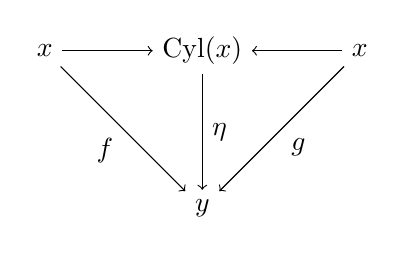
\begin{tikzpicture}
                \node (X) at (-2,0) {$x$};
                \node (X2) at (2,0) {$x$};
                \node (C) at (0,0) {$\mathrm{Cyl}(x)$};
                \node (Y) at (0,-2) {$y$};
                \draw[->] (X) -- (C);
                \draw[->] (X2) -- (C);
                \draw[->] (C) -- node[right]{$\eta$} (Y);
                \draw[->] (X) -- node[below left]{$f$} (Y);
                \draw[->] (X2) -- node[below right]{$g$} (Y);
            \end{tikzpicture}
            \caption{A left homotopy.}
            \label{fig:left_homotopy}
        \end{subfigure}
        \begin{subfigure}[b]{0.49\textwidth}
            \centering
            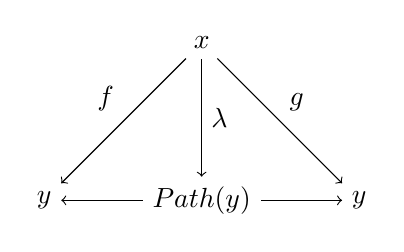
\begin{tikzpicture}
                \node (Y) at (-2,-2) {$y$};
                \node (Y2) at (2,-2) {$y$};
                \node (C) at (0,-2) {$\text{Path}(y)$};
                \node (X) at (0,0) {$x$};
                \draw[<-] (Y) -- (C);
                \draw[<-] (Y2) -- (C);
                \draw[<-] (C) -- node[right]{$\lambda$} (X);
                \draw[<-] (Y) -- node[above left]{$f$} (X);
                \draw[<-] (Y2) -- node[above right]{$g$} (X);
            \end{tikzpicture}
            \caption{A right homotopy.}
            \label{fig:right_homotopy}
        \end{subfigure}
        \caption{Homotopies in a model category.}
    \end{figure}

    \begin{example}[Topological spaces]
        Consider the category $\symbfsf{Top}$. A cylinder object for a topological space $X$ is given by the product $X\times[0,1]$. The codiagonal map is factorized as the endpoint inclusion $X\sqcup X\rightrightarrows X\times[0,1]$ followed by the collapse $X\times[0,1]\overset{\pi_X}{\rightarrow}X$, where it is not hard to show that the collapse is a homotopy equivalence. A left homotopy with respect to $X\times[0,1]$ is exactly a homotopy in the sense of \cref{topology:homotopy}.

        A path object $\mathrm{Path}(X)$ is given by the mapping space $X^{[0,1]}$. The diagonal map is factorized by the basepoint inclusion $X\overset{\iota_0}{\rightarrow}X^{[0,1]}$ followed by the endpoint projections $X^{[0,1]}\rightrightarrows X\times X$. That the right homotopies with respect to $X^{[0,1]}$ give the same equivalence classes as the left homotopies is the content of \cref{topology:path_space}.
    \end{example}

    \begin{property}
        If the domain is cofibrant, every left homotopy induces a right homotopy. Dually, if the codomain is fibrant, every right homotopy induces a left homotopy.
    \end{property}
    \begin{result}[Equivalence relation]
        Whenever the domain $x\in\ob{M}$ is cofibrant and the codomain $y\in\ob{M}$ is fibrant, the relations of being left-homotopic (or, equivalently, right-homotopic) coincide on $\symbfsf{M}(x,y)$ and, in particular, define equivalence relations. The equivalence classes are denoted by $[x,y]$.
    \end{result}

    \begin{property}[Stability under composition]
        Homotopies are preserved under both precomposition and postcomposition by arbitrary morphisms.
    \end{property}
    \begin{property}[Weak equivalences]\label{model:weak_equivalence_homotopy}
        A morphism is a weak equivalence if and only if it is a homotopy inverse.
    \end{property}

    \newdef{Homotopy equivalence}{\index{homotopy!equivalence}
        Two objects $x,y\in\ob{M}$ in a model category are said to be homotopy equivalent if there exists morphisms $f:x\leftrightarrows y:g$ such that $f\circ g$ and $g\circ f$ are homotopic to the identity. The morphisms $f,g$ are then said to be homotopy equivalences.
    }

    In \cref{model:localization}, it was shown that one can assign to every category with weak equivalences a homotopy category. When the category has the additional structure of a model category, one can construct an equivalent category.
    \newadef{Homotopy category II}{\index{homotopy!category}\label{model:homotopy_category_2}
        The homotopy category $\symbfsf{Ho(M)}$ of a model category $\symbfsf{M}$ is the category defined by the following data:
        \begin{itemize}
            \item\textbf{Objects}: $\ob{M}$, and
            \item\textbf{Morphisms}: $\symbfsf{Ho(M)}(x,y) := [x^{\mathrm{cf}},y^{\mathrm{cf}}]$.
        \end{itemize}
    }
    In fact, it is easier to restrict to the subcategory $\symbfsf{M_{cf}}$ of $\symbfsf{Ho(M)}$ on the fibrant-cofibrant objects due to the following property (when restricting to a subcategory, the resulting homotopy category is only equivalent and not isomorphic to the localization).
    \begin{property}
        The homotopy category of a model category is equivalent to those of the full subcategories on (co)fibrant objects:
        \begin{gather}
            \symbfsf{Ho(M)}\cong\symbfsf{Ho(M_f)}\cong\symbfsf{Ho(M_c)}\cong\symbfsf{Ho(M_{cf})}.
        \end{gather}
    \end{property}

    The following theorem gives a stronger version of \cref{model:weak_equivalence_homotopy} above.
    \begin{theorem}[Whitehead]\index{Whitehead}
        A weak equivalence between objects that are both fibrant and cofibrant is a homotopy equivalence.
    \end{theorem}

    \begin{property}
        A Quillen equivalence of model categories induces an equivalence of homotopy categories.
    \end{property}

    \begin{property}[Monoidal model categories]
        The homotopy category of a monoidal model category has a closed monoidal structure defined by the induced derived adjunction. The homotopy category of an enriched model category is enriched, powered and copowered over the homotopy category of its enriching category, where the enriched structure is again given by the induced derived adjunction.
    \end{property}

    In some cases, it is useful to consider categories that are strictly weaker than model categories but stronger than categories with weak equivalences. The prime example being the full subcategories of a model category on the (co)fibrant objects. These are often easier to handle in the setting of homotopy theory.
    \newdef{Category of fibrant objects}{\index{fibrant object}\index{fibration}
        A category $\symbfsf{C}$ with weak equivalences $\symbfsf{W}\hookrightarrow\symbfsf{C}$ equipped with another subcategory $\symbfsf{F}\hookrightarrow\symbfsf{C}$ for which the morphisms are called \textbf{fibrations} such that the following conditions are satisfied:
        \begin{enumerate}
            \item $\symbfsf{C}$ has finite products.
            \item Fibrations and acyclic fibrations are preserved under arbitrary pullbacks.
            \item Every object admits a good path object.
            \item All objects are fibrant.
        \end{enumerate}
    }

    \begin{theorem}[Factorization lemma]\index{factorization!lemma}
        In a category of fibrant objects, any morphism can be factorized as the right inverse of an acyclic fibration followed by a fibration.
    \end{theorem}

    The following theorem is important for characterizing functors that preserve weak equivalences.
    \begin{theorem}[Ken Brown's lemma]\index{Ken Brown}\label{model:ken_brown}
        Let $\symbfsf{C}$ be a category of fibrant objects and let $\symbfsf{D}$ be a category with weak equivalences. If a functor $\func{F}{C}{D}$ maps acyclic fibrations to weak equivalences, it preserves all weak equivalences.
    \end{theorem}
    \remark{An analogous theorem exists for \textit{categories of cofibrant objects}.}

    The above lemma allows to define derived functors for Quillen functors between model categories (the following definition is also better suited for working in the $\infty$-setting than \cref{model:derived_functor}).
    \newadef{Derived functor}{\index{derived!functor}\label{model:derived_functor_replacement}
        Let $\func{F}{C}{D}$ be a left (resp.~right) Quillen functor. The left (resp.~right) derived functors are obtained by precomposition with the cofibrant (resp.~fibrant) replacement functors.
    }
    \begin{property}[Derived functors are absolute]\label{model:absolute_derived_functors}
        It can be shown that derived functors built using (co)fibrant replacement are given by absolute Kan extensions. So, even though homotopy categories often do not admit all (co)limits, the resulting Kan extensions do exist.
    \end{property}

\subsection{\difficult{Reedy model structure}}

    Consider a bicomplete category $\symbfsf{M}$ (this will often be $\symbfsf{sSet}$). For any full subcategory inclusion $\symbfsf{D}\hookrightarrow\symbfsf{C}$, one obtains an induced \textbf{truncation} (or \textbf{restriction}) functor $\tr:\symbfsf{M^C}\rightarrow\symbfsf{M^D}$. The left and right adjoints of this functor are, respectively, called the \textbf{skeleton} and \textbf{coskeleton} functors.
    \begin{formula}
        The adjoint functors are defined by Kan extensions and, hence, can be expressed in terms of (co)ends and weighted (co)limits:
        \begin{gather}
            \begin{aligned}
                \mathrm{sk}(X)x &:= \int^{y\in\symbfsf{D}}\symbfsf{C}(y,x)\cdot Xy = \colim^{\symbfsf{C}(-,x)}X\,,\\
                \mathrm{cosk}(X)x &:= \int_{y\in\symbfsf{D}}\bigl[\symbfsf{C}(x,y),Xy\bigr] = \wlim{\symbfsf{C}(x,-)}X.
            \end{aligned}
        \end{gather}
    \end{formula}
    \newdef{Skeletal sets}{\index{skeleton}
        Let $\symbfsf{M}=\symbfsf{sSet}$ and consider the inclusion $\simplex_{\leq n}\hookrightarrow\simplex$ of the full subcategory on the objects $\{[0],\ldots,[n]\}$. The $n$-truncation functor $\tr_n$ discards all simplices of degree higher than $n$ or, in other words, it `truncates' a simplicial set at degree $n$.

        The $n$-skeleton functor $\mathrm{sk}_n$ takes a simplicial set $X$ of degree $\leq n$ and freely adds degenerate simplices in degrees $>n$, i.e.~it is the smallest simplicial set containing $X$ as a simplicial subset. The $n$-coskeleton functor $\mathrm{cosk}_n$ adds a simplex in degree $>n$ whenever all of its faces are present, i.e.~the $m$-simplices in $\text{cosk}_nX$ are given by the collection of all $(m+1)$-tuples of $(m-1)$-simplices that are compatible (along lower simplices).
    }
    \begin{property}[Simplicial nerve]\index{nerve}
        The nerve functor $\func{N}{Cat}{sSet}$ from \cref{model:nerve} is a fully faithful functor to the category of 2-coskeletal simplicial sets. This follows from the fact that, in ordinary categories, compositions of morphisms are unique and, hence, all higher-order tuples of composable morphisms are determined by composable pairs. In fact, this is just the characterization of (small) categories as categories internal to $\symbfsf{Set}$ (under the isomorphism $C_2\cong C_1\times_{C_0}C_1$ which will be called the first \textit{Segal condition} in \cref{model:segal_space}).
    \end{property}

    \newdef{Reedy category}{\index{Reedy!category}\label{model:reedy}
        A category $\symbfsf{R}$ equipped with a \textbf{degree} function $\ob{R}\rightarrow\alpha$, where $\alpha$ is an ordinal (\cref{set:ordinal}), and two wide subcategories $\symbfsf{R}^\pm$ that satisfy the following conditions:
        \begin{enumerate}
            \item Nontrivial morphisms in $\symbfsf{R}^+$ (strictly) increase the degree.
            \item Nontrivial morphisms in $\symbfsf{R}^-$ (strictly) decrease the degree.
            \item All morphisms admit a unique factorization as a morphism in $\symbfsf{R}^-$ followed by a morphism in $\symbfsf{R}^+$. This factorization is sometimes called the \textbf{(canonical) Reedy factorization}.
        \end{enumerate}
    }

    \begin{property}[Minimality]\index{degree!of factorization}
        The Reedy factorization is the (unique) factorization of minimal degree, where the \textbf{degree} of a factorization $x\overset{f}{\rightarrow}y\overset{g}{\rightarrow}z$ is defined as the degree of $y$.
    \end{property}
    \begin{property}[Isomorphisms are trivial]
        A morphism in a Reedy category is an isomorphism if and only if it is trivial.
    \end{property}

    \begin{example}
        Some common examples of Reedy categories are discrete categories, finite posets, the simplex category $\simplex$ and opposites of Reedy categories.
    \end{example}

    For Reedy categories, one can also define $n$-truncation, $n$-skeleton and $n$-coskeleton functors by restricting to the full subcategories on elements of degree $\leq n$.
    \newdef{Matching and latching objects}{\index{matching!object}\index{latching object}
        Let $\symbfsf{R}$ be a Reedy category and consider a diagram $X\in\funccat{R}{C}$ with $\symbfsf{C}$ small. Consider the skeleton monad and coskeleton comonad (often just called the skeleton and coskeleton functors) $\symbfsf{sk}_n:=\mathrm{sk}_n\circ\tr_n$ and $\symbfsf{cosk}_n:=\mathrm{cosk}_n\circ\tr_n$. The latching and matching objects of $X$ at $r\in\ob{R}$ are defined as the restrictions of $\symbfsf{sk}_{\deg(r)-1}$ and $\symbfsf{cosk}_{\deg(r)-1}$ to the degree-$\deg(r)$ subcategory of $\symbfsf{R}$, respectively. The counits of these adjunctions give rise to the \textbf{latching} and \textbf{matching} maps.

        One can also define the latching and matching objects through (co)limits. Define the subcategory $\symbfsf{R}^+(r)$ as the subcategory of $\symbfsf{R}^+/r$ on all objects except the identity. The latching object $L_rX$ can be shown to be isomorphic to the colimit of $X$ over $\symbfsf{R}^+(r)$.
    }

    \begin{example}[Simplicial objects]\index{simplicial!object}\index{Eilenberg--Zilber}
        The above property allows to give a nice interpretation to latching objects in the case of $\symbfsf{R}=\simplex^{\text{op}}$. Using the \textit{Eilenberg--Zilber lemma}, it can be shown that the $n^{\text{th}}$ latching object of a simplicial object is given by its collection of degenerate $n$-simplices.
    \end{example}

    \newdef{Boundary}{\index{boundary}
        The boundary of a representable presheaf $\symbfsf{R}(-,r)$, denoted by $\partial\symbfsf{R}(-,r)$, is defined as its latching object. It can be shown that $\partial\symbfsf{R}(-,r)$ consists of exactly those morphisms that are not in $\symbfsf{R}^-$.
    }
    \begin{formula}
        One can show that the latching and matching objects can be obtained through (co)limits weighted by boundaries:
        \begin{gather}
            \label{model:latching_boundary}
            \begin{aligned}
                M_rX &\cong \wlim{\partial\symbfsf{R}(r,-)}X\,,\\
                L_rX &\cong \colim^{\partial\symbfsf{R}(-,r)}X\,.
            \end{aligned}
        \end{gather}
    \end{formula}

    From here on, $\symbfsf{M}$ will be assumed to be a model category. In this case, a canonical model structure on the functor category $\funccat{R}{M}$ for Reedy $R$ can be defined.
    \newdef{Relative matching and latching objects}{
        Consider the (weighted) colimit bifunctor
        \begin{gather}
            \func{\text{colim}}{Psh(R)\times[R,M]}{M}\,.
        \end{gather}
        The Leibniz construction~\ref{model:pushout_product} allows to define the relative latching object of $f:X\rightarrow Y$ at $r\in\ob{R}$ as the Leibniz product of the boundary inclusion $\partial\symbfsf{R}(-,r)\hookrightarrow\symbfsf{R}(-,r)$ and $f$.

        By \namecrefs{cat:weighted_hom_colimit}~\eqref{cat:weighted_hom_colimit} and~\eqref{model:latching_boundary}, the relative latching map is of the form $Xr\sqcup_{L_rX}L_rY\rightarrow Yr$ and the relative matching map is of the form $Xr\rightarrow Yr\times_{M_rY}M_rX$.
    }

    \begin{property}[Reedy model structure]\index{Reedy!model structure}
        Let $\symbfsf{R}$ be a Reedy category and let $\symbfsf{M}$ be a model category. The functor category $\funccat{R}{M}$ admits the following model structure:
        \begin{itemize}
            \item\textbf{Weak equivalences}: the objectwise weak equivalences.
            \item\textbf{Fibrations}: morphisms for which the relative matching map is a fibration (in $\symbfsf{M}$) for all $r\in\ob{R}$
            \item\textbf{Cofibrations}: morphisms for which the relative latching map is a cofibration (in $\symbfsf{M}$) for all $r\in\ob{R}$
        \end{itemize}
    \end{property}

    \begin{property}[Quillen (co)limit functors]
        Consider a $\mathcal{V}$-enriched model category $\symbfsf{M}$ and a Reedy category $\symbfsf{R}$. For every Reedy cofibrant functor $W$ in $\funccat{R}{\mathcal{V}}$, the weighted limit and colimit functors are right and left Quillen, respectively.
    \end{property}

    \todo{COMPLETE (this section is too abstract and difficult at this point, a more intuitive explanation of matching/latching objects is necessary)}

\section{Simplicial spaces}
\subsection{Kan complexes}

    \newdef{Horn}{\index{horn}
        Consider the standard simplex $\Delta[n]$. For all $n\geq1$ and $0\leq k\leq n$, the $(n,k)$-horn $\Lambda^k[n]$ is defined as the subsimplicial set obtained by removing the $k^{\text{th}}$ face from $\partial\Delta[n]$. When $k=0$ or $k=n$, the horn is said to be \textbf{outer}, otherwise it is said to be \textbf{inner}.
    }

    \newdef{Kan fibration}{\index{Kan!fibration}
        A morphism of simplicial sets that has the right lifting property with respect to all horn inclusions $\Lambda^k[n]\hookrightarrow\Delta[n]$.
    }
    \newdef{Kan complex}{\index{Kan!complex}\label{model:kan_complex}
        A simplicial set that has all horn fillers or, equivalently, a simplicial set for which the terminal morphism is a Kan fibration. The full subcategory of $\symbfsf{sSet}$ on Kan complexes is denoted by $\symbfsf{Kan}$.
    }

    \begin{property}[Horn filler condition]\label{model:horn_filler}
        A simplicial set is the nerve of a (small) category if and only if all of its inner horns admit a unique filler (compositions are unique). If one requires all horns to admit a unique filler, the nerve of a groupoid is obtained.
    \end{property}

    By relaxing the above requirements, one can generalize the notion of a category (this is due to \textit{Boardman} and \textit{Vogt}).
    \newdef{Quasicategory\footnotemark}{\index{quasi-!category}\index{logos}\index{Boardman condition}\label{model:quasicategory}
        \footnotetext{Some authors, such as \textit{Joyal}, call these \textbf{logoi} (singular: \textbf{logos}).}
        A simplicial set for which all inner horns have (not necessarily unique) fillers. This condition is sometimes called the \textbf{Boardman condition}.
    }

    At this point, a third instance of a `homotopy category' can be defined.
    \newdef{Homotopy category III}{\index{homotopy!category}
        Let $X$ be a quasicategory. The homotopy category $\symbfsf{Ho}(X)$ consists of the following data:
        \begin{itemize}
            \item\textbf{Objects}: $X_0$.
            \item\textbf{Morphisms}: The quotient of $X_1$ under the relation $f\circ g\sim h$ if there exists a 2-simplex with (suitably oriented) edges $f,g$ and $h$.
        \end{itemize}
    }
    \begin{property}[Fundamental category]\index{fundamental!category}
        If $X$ is a quasicategory, its homotopy category is equivalent to its \textbf{fundamental category} $\pi_1(X)$, i.e.~the image under the left adjoint of the (simplicial) nerve functor.
    \end{property}

    The following theorem is a restatement of \cref{model:horn_filler}.
    \begin{theorem}[Joyal]\index{Joyal}
        A quasicategory is a Kan complex if and only if its homotopy category is a groupoid.
    \end{theorem}

\subsection{Simplicial localization}

    \newdef{Homotopy category IV}{\index{homotopy!category}\label{model:enriched_homotopy_category}
        Consider a simplicially enriched category $\symbfsf{C}$. Its homotopy category $\pi_0(\symbfsf{C})$ is defined as follows:
        \begin{itemize}
            \item\textbf{Objects}: $\ob{C}$, and
            \item\textbf{Morphisms}: $\pi_0\symbfsf{C}(x,y)$.
        \end{itemize}
        Two morphism $f,g\in\symbfsf{C}(x,y)$ are said to be \textbf{homotopic} if they are identified in $\pi_0(\symbfsf{C})$. A morphism $f\in\symbfsf{C}(x,y)$ is called a \textbf{homotopy equivalence} if it admits both a left and a right inverse in $\pi_0(\symbfsf{C})$, i.e.~if it becomes an isomorphism in the homotopy category.
    }
    \newdef{Dwyer--Kan equivalence I}{\index{equivalence!Dwyer--Kan}\label{model:enriched_dwyer_kan}
        Consider a simplicial functor $\func{F}{C}{D}$ between two simplicially enriched categories. This functor is called a Dwyer--Kan equivalence if:
        \begin{itemize}
            \item $F$ is \textbf{$\infty$-fully faithful}, i.e.~the induced map on hom-objects is a weak equivalence.\footnote{This is a generalization of the ordinary definition for categories. (Simplicial categories will give models for \textit{$\infty$-categories.})}
            \item The induced map on connected components $\pi_0( F):\pi_0(\symbfsf{C})\rightarrow\pi_0(\symbfsf{D})$ is an equivalence (of categories). In fact, this condition can be relaxed to $\pi_0(F)$ being essentially surjective, since together with the previous condition this implies that $\pi_0(F)$ is an equivalence.
        \end{itemize}
    }

    \begin{construct}[Hammock localization]\index{localization!hammock}\index{simplicial!localization}
        The hammock localization (or \textbf{simplicial localization}) $L^H\symbfsf{C}$ of a category with weak equivalences $(\symbfsf{C},W)$ is the simplicially enriched category constructed as follows:
        \begin{itemize}
            \item\textbf{Objects}: $\ob{C}$, and
            \item\textbf{Morphisms}: $L^H\symbfsf{C}(x,y)$ is the simplicial set defined as follows:
            \begin{quote}
                First, for every $n\in\mathbb{N}$, one constructs a category with as objects the zigzags of morphisms in $\symbfsf{C}$ relating $x$ and $y$ such that all left-pointing morphisms are in $W$, and as morphisms the endpoint-preserving `natural transformations' (in the sense that all triangles/squares in the resulting diagram commute). Then, the coproduct is taken over the (simplicial) nerves of the categories for all $n\in\mathbb{N}$. Finally, the quotient is taken by the equivalence relations generated by:
                \begin{enumerate}
                    \item inserting or removing identity morphisms, and
                    \item composing morphisms.
                \end{enumerate}
            \end{quote}
        \end{itemize}
    \end{construct}

    The following property relates all constructions of what could be called homotopy categories.
    \begin{property}
        Let $(\symbfsf{C},W)$ be a category with weak equivalences. It can be shown that
        \begin{gather}
            \symbfsf{Ho}(L^H\symbfsf{C})\cong\symbfsf{C}[W^{-1}]\,.
        \end{gather}
        This construction gives a more explicit description of the homotopy category. Furthermore, if $\symbfsf{M}$ is a simplicial model category, the categories $\symbfsf{M_{cf}}$ and $L^H\symbfsf{M}$ are Dwyer--Kan equivalent.
    \end{property}
    \begin{property}
        Quillen equivalent model categories have Dwyer--Kan equivalent simplicial localizations.
    \end{property}

    \begin{property}\label{model:all_simplicial_localization}
        Up to Dwyer--Kan equivalence, every simplicially enriched category can be obtained as the simplicial localization of a category with weak equivalences.
    \end{property}

    \newdef{Simplicial resolution}{\index{resolution!(co)simplicial}
        Consider an object $x\in\ob{M}$ in a model category $\symbfsf{M}$. A (co)simplicial resolution of $x$ is a Reedy (co)fibrant (co)simplicial object $X$ together with a weak equivalence $x\simeq X_0$.

        Every object in a model category admits a (co)simplicial resolution by taking a (co)fibrant replacement of the constant (co)simplicial object.
    }

    \newdef{Bergner model structure}{\index{Bergner model structure}
        The catgory of simplicially enriched categories admits the following model structure:
        \begin{itemize}
            \item\textbf{Weak equivalences}: Dwyer--Kan equivalences,
            \item\textbf{Cofibrant objects}: \textit{simplicial computads}, and
            \item\textbf{Fibrant objects}: $\symbfsf{Kan}$-enriched categories.
        \end{itemize}
    }
    \newconstr{Free resolution}{\index{resolution}\index{computad}\label{model:bergner_free_resolution}
        Consider a (small) category $\symbfsf{C}$. From this category, we can construct a simplicial category $\mathfrak{C}\symbfsf{C}$ consisting of the following data:
        \begin{itemize}
            \item\textbf{Objects}: $\ob{C}$, and
            \item\textbf{Morphisms}: $\mathrm{hom}(\mathfrak{C}\symbfsf{C})_n := \mathrm{hom}(F^{n+1}\symbfsf{C})$, where $F$ is identity-on-objects and $F\symbfsf{C}$ has as morphisms strings of composable morphisms in $\symbfsf{C}$.
        \end{itemize}
        It can be shown that $\mathfrak{C}\symbfsf{C}$ is a \textit{simplicial computad} for any simplicially enriched category $\symbfsf{C}$, $\mathfrak{C}$ acts as the cofibrant replacement functor in the Bergner model structure.
    }

\subsection{Segal spaces}

    \begin{example}[Bisimplicial sets]
        Simplicial objects in $\symbfsf{sSet}$ are, in particular, also $\symbfsf{sSet}$-enriched and, accordingly, such objects are often called bisimplicial sets or \textbf{simplicial spaces}\footnote{The latter name follows from the fact that topological spaces and simplicial sets are (Quillen-)equivalent.}. Since $\symbfsf{sSet}$ is a model category, \cref{model:model_functor_category} above says that $\symbfsf{ssSet}$ itself admits a model structure. It can furthermore be shown that the injective model structure on $\symbfsf{ssSet}$ coincides with the Reedy model structure (a rather nontrivial statement).
    \end{example}

    \newdef{Segal space}{\index{Segal!space}\index{Segal!condition}\index{spine}\label{model:segal_space}
        Consider a fibrant object $X$ in the injective model structure on $\symbfsf{ssSet}$. This bisimplicial set is called a Segal space if it satisfies the following weak form of the \textbf{Segal condition} for all $n\geq1$:\footnote{If the Reedy condition is omitted, the limit on the right-hand side has to be replaced by a \textit{homotopy limit}.}
        \begin{gather}
            X_n\simeq\underbrace{X_1\times_{X_0}\cdots\times_{X_0}X_1}_{n\text{ times}}\,.
        \end{gather}
        These maps are called \textbf{Segal maps} (even when they are not weak equivalences). They are the morphisms induced by \textbf{spine} inclusions, i.e.~inclusions of the union of edge 1-cells.
    }
    \newdef{Segal category}{\index{Segal!category}
        A bisimplicial set $X$ is called a \textbf{Segal precategory} if $X_0$ is discrete. It is called a Segal category if, in addition, all its Segal maps are weak equivalences, i.e.~if it is a Segal space with a discrete set of `objects'.
    }

    \newdef{Mapping space}{\index{mapping!space}
        Consider a Segal space $X$. For every two points $x,y\in X_0$, the mapping space $\mathrm{Map}(x,y)$ is defined as the fibre of $(d_1,d_0):X_1\rightrightarrows X_0\times X_0$ over the point $(x,y)$. The identity at $x\in X_0$ is given by $s_0(x)$.
    }

    The following two definitions should be compared to \namecrefs{model:enriched_homotopy_category}~\ref{model:enriched_homotopy_category} and~\ref{model:enriched_dwyer_kan}.
    \newdef{Homotopy category V}{\index{homotopy!category}
        Consider a Segal category $X$. Its homotopy category $\symbfsf{Ho}(X)$ is defined as follows:
        \begin{itemize}
            \item\textbf{Objects}: $X_0$, and
            \item\textbf{Morphisms}: $\pi_0\mathrm{Map}(x,y)$.
        \end{itemize}
        Two points $f,g\in\mathrm{Map}(x,y)$ are said to be \textbf{homotopic} if they are identified in $\symbfsf{Ho}(X)$. A point $f\in\mathrm{Map}(x,y)$ is called a \textbf{homotopy equivalence} if it admits both a left and a right inverse in $\symbfsf{Ho}(X)$, i.e.~if it becomes an isomorphism. The subspace $X_\mathrm{hoequiv}\subset X_1$ consists of the components that contain homotopy equivalences.\footnote{It should be noted that if any point in a component is a homotopy equivalence, all points in that component are homotopy equivalences.}
    }
    \newdef{Dwyer--Kan equivalence II}{\index{equivalence!Dwyer--Kan}
        A map of Segal spaces such that:
        \begin{enumerate}
            \item the induced map on mapping spaces is a weak equivalence, and
            \item the induced map between homotopy categories is an equivalence (of categories).
        \end{enumerate}
    }

    \newdef{Complete Segal space}{\index{Segal!space}
        A Segal space $X$ for which the map $s_0:X_0\rightarrow X_\mathrm{hoequiv}$ is a weak equivalence.
    }
    \begin{property}[Dwyer-Kan equivalence]
        A map of Segal spaces is a Dwyer--Kan equivalence if and only if it is a weak equivalence in the \textit{complete Segal space model structure}. A map of complete Segal spaces is a Dwyer--Kan equivalence if and only if it is a levelwise weak equivalence.
    \end{property}

\subsection{Coherent nerve}

    The nerve and realization functors (\cref{model:nerve_and_realization}) can also be modified to incorporate the higher homotopical data present in a simplicially enriched category.

    First, define a cosimplicial simplicially enriched category $\func{C}{\simplex}{sSetCat}$ that assigns to every finite ordinal $[n]$, the category consisting of the following data:
    \begin{itemize}
        \item\textbf{Objects}: $[n]\equiv\{0,1,\ldots,n\}$, and
        \item\textbf{Morphisms}: $C[n](i,j) := N(P_{ij})$, where $N$ is the ordinary nerve functor on $\symbfsf{Cat}$ and $P_{ij}$ is the poset consisting of all subsets of $\{i,\ldots,j\}$ that contain both $i$ and $j$.
    \end{itemize}
    The (homotopy) \textbf{coherent nerve functor} (or \textbf{simplicial nerve functor}\footnote{This terminology was also used for the ordinary nerve functor taking values in $\symbfsf{sSet}$. In general, it should be clear from the context which one is meant.}) is the nerve functor induced by this cosimplicial object. It not only knowns about all possible morphisms, it also knows about all possible ways how one can obtain this morphism.
    \begin{remark}
        The cosimplicial object $\func{C}{\simplex}{sSetCat}$ is in fact just the free resolution functor $\mathfrak{C}$ in the Bergner model structure (\cref{model:bergner_free_resolution}) restricted to the subcategory $\simplex$.
    \end{remark}

    \begin{property}
        The homotopy coherent nerve functor $N_{\simplex}$ is uniquely determined by the following relation:
        \begin{gather}
            \symbfsf{sSet}(\Delta[n],N_\Delta\symbfsf{C})=\symbfsf{sSetCat}(C[n],\symbfsf{C})\,.
        \end{gather}
    \end{property}

    \begin{property}[Simplicial realization]
        The left adjoint of the homotopy coherent nerve functor satisfies the following relation for all finite ordinals $[n]$:
        \begin{gather}
            |\Delta[n]|\cong C[n]\,.
        \end{gather}
    \end{property}

    \begin{property}[Quasicategories]
        If $\symbfsf{C}$ is $\symbfsf{Kan}$-enriched, its coherent nerve is a quasicategory. By \cref{model:simplicial_model_category}, this allows to associate a quasicategory to any simplicial model category by passing to the coherent nerve of its fibrant-cofibrant subcategory.
    \end{property}

    At this point, it is interesting to reconsider the simplicial nerve construction (\cref{model:nerve}). Although the functor $\func{N}{Cat}{sSet}$ is fully faithful, there is a problem in that weak equivalences of simplicial sets do not necessarily correspond to (weak) equivalences of categories. The issue comes from the definition of the canonical model structure (\cref{model:sset_model_structure}) on $\symbfsf{sSet}$. Here, the weak equivalences are those morphisms that become weak equivalences after geometric realization. During this step, information about the direction of morphisms is lost and it becomes impossible to distinguish categories from groupoids. Only when all morphisms are assumed to be invertible, i.e.~the category is assumed to be a groupoid, does one recover the converse statement.

    A first solution is to use a different model structure with less weak equivalences.
    \newdef{Joyal model structure}{\index{Joyal!model structure}
        $\symbfsf{sSet}$ admits a model structure defined by the following data:
        \begin{itemize}
            \item\textbf{Weak equivalences}: \textit{weak categorical equivalences}, i.e.~maps $f:X\rightarrow Y$ such that the induced simplicial functor $C(f):C(X)\rightarrow C(Y)$ is a Dwyer--Kan equivalence.
            \item\textbf{Cofibrations}: monomorphisms.
            \item\textbf{Fibrant objects}: quasicategories (\cref{model:quasicategory}).
        \end{itemize}
    }
    When characterizing those simplicial sets that are nerves of categories, groupoids and categories are distinguished by whether all horns admit a (unique) filler or only inner horns admit a (unique) filler. However, when the fibrant objects ar<e Kan complexes, those simplicial sets that admit all horn fillers, the homotopical structure only knows about nerves that come from a groupoid. By passing to the larger class of quasicategories, this problem is solved.

    Instead of changing the model structure on $\symbfsf{sSet}$ to overcome the issues with taking nerves of categories or groupoids, one can also change the construction of the nerve functor. An alternative approach was introduced by \textit{Rezk}.
    \newdef{Classifying diagram}{\index{classifying!diagram}
        Consider a (small) category $\symbfsf{C}$ together with the functor category $\symbfsf{C}^{[n]}$. The classifying diagram of $\symbfsf{C}$ is the bisimplicial set $\widetilde{N}\symbfsf{C}$ defined levelwise as follows:
        \begin{gather}
            \widetilde{N}\symbfsf{C}_k := N\bigl(\mathrm{Core}(\symbfsf{C}^{[k]})\bigr)\,,
        \end{gather}
        where $N$ is the ordinary nerve functor and $\mathrm{Core}$ denotes the core of a category (\cref{cat:core}).

        The reason for why this construction is better for distinguishing categories stems from the fact that information about isomorphisms is already captured at degree 0, while information about noninvertible morphisms is only captured from degree 1 onwards.
    }
    \begin{property}
        If $\symbfsf{C}$ is small, then $\widetilde{N}\symbfsf{C}$ is a complete Segal space.
    \end{property}

    \todo{COMPLETE}

\section{Cofibrantly generated categories}
\subsection{Transfinite constructions}

    Before proceeding, some notions from ordinary category need to be specialized to the context of regular cardinals (\cref{set:regular_cardinal}). In this section, the symbol $\kappa$ will always denote such a regular cardinal.

    \newdef{$\kappa$-filtered category}{\index{category!filtered}
        A category in which every diagram with less than $\kappa$ arrows admits a cocone.
    }

    \newdef{$\kappa$-directed limit}{\index{limit!directed}
        Consider a poset $I$ such that every subposet of cardinality less than $\kappa$ has a lower bound (upper bound for directed colimits). Such a set is said to be $\kappa$-(co)directed. A limit of a diagram over this poset is called a $\kappa$-(co)directed (co)limit.
    }

    The following definition is a categorification of the previous one.
    \newdef{$\kappa$-filtered limit}{\index{limit!filtered}
        Consider a diagram $\func{D}{I}{C}$. The limit (resp.~colimit) of $D$ is said to be $\kappa$-cofiltered (resp.~$\kappa$-filtered) if $\symbfsf{I}$ is a $\kappa$-cofiltered (resp.~$\kappa$-filtered) category.

        It should be noted that an analogue of \cref{cat:directed_filtered} also holds in the $\kappa$-context, i.e.~a category has all $\kappa$-directed limits if and only if it has all $\kappa$-filtered limits (and analogously for colimits).
    }

    \newdef{Small object}{\index{small}\index{presentable}
        An object for which there exists a regular cardinal $\kappa$ such that its covariant hom-functor preserves all $\kappa$-filtered colimits. These objects are also said to be \textbf{$\kappa$-compact} or \textbf{$\kappa$-presentable} (cf.~\cref{cat:compact}).
    }
    
    \newdef{Accessible category}{\index{accessible}
        A locally small category $\symbfsf{C}$ for which there exists a regular cardinal $\kappa$ such that $\symbfsf{C}$ has all $\kappa$-filtered colimits and such that it is generated under $\kappa$-filtered colimits by a small subcategory $\symbfsf{D}$ of $\kappa$-small objects, i.e.~$\symbfsf{C}\cong\mathrm{Ind}_\kappa(\symbfsf{D})$.
    }
    \begin{adefinition}
        A category equivalent to the category of ($\kappa$-)flat functors (\cref{topos:flat_functor}) on a small category or, by \cref{topos:flat_or_ind}, the category of ($\kappa$)ind-objects on a small category.
    \end{adefinition}


    \newdef{Locally presentable category}{\index{presentable}
        A cocomplete, accessible category. It can be shown that such categories are also complete and, hence, bicomplete.
    }

    \begin{property}
        Every locally presentable category can be obtained as a full reflective subcategory of a presheaf category under an \textbf{accessible embedding}, i.e.~a finitary embedding of accessible categories.
    \end{property}
    \begin{property}[Gabriel--Ulmer duality]\index{Gabriel--Ulmer duality}
        First, define the following two 2-categories. $\symbfsf{LFP}$ consists of the following data:
        \begin{itemize}
            \item\textbf{Objects}: locally finitely presentable categories,
            \item\textbf{1-Morphisms}: finitary, right adjoint functors (\cref{cat:finitary_functor}), and
            \item\textbf{2-Morphisms}: natural transformations.
        \end{itemize}
        $\symbfsf{Lex}$ consists of the following data:
        \begin{itemize}
            \item\textbf{Objects}: small, finitely complete categories,
            \item\textbf{1-Morphisms}: left exact functors, and
            \item\textbf{2-Morphisms}: natural transformations.
        \end{itemize}
        There exists an equivalence $\op{\symbfsf{Lex}}\cong\symbfsf{LPF}$ that sends a small, finitely complete category to its category of left exact copresheaves.
    \end{property}

    \begin{theorem}[Adjoint functor theorem]\index{adjoint functor theorem}\label{cat:adjoint_functor_theorem}
        Consider a functor $\func{F}{C}{D}$ between locally presentable categories. $F$ admits a right adjoint if and only if it preserves all colimits. $F$ admits a left adjoint if and only if it is accessible and if it preserves all limits.
    \end{theorem}

    For ordinary categories, the axioms guarantee the existence of a (unique) composition of any finite number of (composable) morphisms. However, in some cases it is useful, or even necessary, to talk about the `composite' of an infinite number of morphisms.
    \newdef{Transfinite composition}{\index{composition}\index{continuous}\label{cat:transfinite_composition}
        Consider a category $\symbfsf{C}$ with a collection of morphisms $I\subseteq\mathrm{hom}(\symbfsf{C})$ and let $\alpha$ be an infinite ordinal. An $\alpha$-indexed \textbf{transfinite sequence} of morphisms in $I$ is a diagram of the form $D:\alpha\rightarrow\symbfsf{C}$ such that:
        \begin{enumerate}
            \item Successor morphisms in $\alpha$ are mapped to elements of $I$.
            \item $D$ is `continuous' in the sense that for every limit ordinal $\beta<\alpha$: $D\beta\cong\underset{\gamma<\beta}{\colim}\ D\gamma$.
        \end{enumerate}
        $D\lambda$ denotes the restriction of $D$ to the (full) subdiagram $\{\gamma\mid\gamma<\lambda\}$ of $\alpha$. The transfinite composition of this sequence is the induced morphism $D_0\rightarrow D\alpha\equiv\colim\ D$.
    }
    \newdef{Cell complex}{\index{cell!complex}
        Consider a cocomplete category $\symbfsf{C}$ with a collection of morphisms $I\subseteq\mathrm{hom}(\symbfsf{C})$. A \textbf{relative} $I$-cell complex is a transfinite composition of pushouts (of coproducts\footnote{It can be shown that closure under coproducts follows automatically.}) of morphisms in $I$. An $I$-cell complex is an object such that the unique morphism from the initial object is a relative $I$-cell complex.
    }
    \newnot{Relative cell complexes}{
        The set of all relative $I$-cell complexes is often denoted by $\mathrm{cell}(I)$.
    }

\subsection{Cofibrant generation}

    \newdef{Saturated class}{\index{saturated}
        A collection of morphisms $I\subseteq\mathrm{hom}(\symbfsf{C})$ in a category is said to be \textbf{(weakly) saturated} if it is closed under:
        \begin{enumerate}
            \item pushouts,
            \item retracts (in the arrow category of $\symbfsf{C}$), and
            \item transfinite compositions.
        \end{enumerate}
    }

    \newdef{Cofibrantly generated WFS}{\index{cofibrantly generated}
        A weak factorization system $(R,L)$ on a category $\symbfsf{C}$ (\cref{model:wfs}) is said to be cofibrantly generated by a collection of morphisms $I\subseteq\mathrm{hom}(\symbfsf{C})$ if
        \begin{gather}
            R=\mathrm{rlp}(I)\,.
        \end{gather}
    }

    The following is a famous result by \textit{Quillen}.\index{Quillen}
    \begin{theorem}[Small object argument]\index{small!object argument}
        Let $\symbfsf{C}$ be a locally presentable category with a set of morphisms $I\subseteq\mathrm{hom}(\symbfsf{C})$. The WFS given by $\mathrm{llp}(I)=\mathrm{cell}(I)$ is cofibrantly generated.
    \end{theorem}
    \begin{remark}
        This theorem can be generalized to cocomplete categories where the domains of morphisms in $I$ are small relative\footnote{\textit{Small relative to a set of morphisms} is defined just as ordinary smallness, but with general $\kappa$-filtered colimits replaced by those that start from morphisms in the given set.} to $\mathrm{cell}(I)$. Sets of morphisms with this property are said to \textbf{admit a small object argument}.
    \end{remark}

    \newdef{Cofibrantly generated model category}{\index{model!category}
        A model category $\symbfsf{C}$ is said to be cofibrantly generated by two sets of morphisms $I,J\subseteq\mathrm{hom}(\symbfsf{C})$ if it satisfies the following conditions:
        \begin{enumerate}
            \item $I$ and $J$ both admit the small object argument.
            \item The fibrations are given by $\mathrm{rlp}(J)$.
            \item The acyclic fibrations are given by $\mathrm{rlp}(I)$.
        \end{enumerate}
        It can be shown that the last two conditions are equivalent to the following ones:
        \begin{enumerate}
            \item[$2^*.$] The cofibrations are the retracts (in the arrow category) of $\mathrm{cell}(I)$.
            \item[$3^*.$] The acyclic cofibrations are the retracts (in the arrow category) of $\mathrm{cell}(J)$.
        \end{enumerate}
        The morphisms in $I$ and $J$ are called the \textbf{generating cofibrations} and \textbf{generating acyclic cofibrations}, respectively.
    }

    Sometimes, it is desirable to replace the model structure on a category $\symbfsf{C}$ by one that has more weak equivalences (denote the new one by $\symbfsf{C}_0$). If the cofibrations remain the same, this new structure has some nice properties:
    \begin{itemize}
        \item The fibrations are a subclass of the original ones.
        \item The acyclic fibrations remain the same.
        \item The identity functors $\mathbbm{1}_{\symbfsf{C}_0}:\symbfsf{C}_0\leftrightarrows\symbfsf{C}:\mathbbm{1}_{\symbfsf{C}}$ form a Quillen adjunction.
        \item Every object in $\symbfsf{C}$ is weakly equivalent (in $\symbfsf{C}_0$) to one in $\symbfsf{C}_0$.
    \end{itemize}

    This procedure can be made explicit for a specific class of model categories. Let $\symbfsf{C}$ be a left proper, cofibrantly generated, simplicial model category and consider a collection $S\subset\mathrm{hom}(\symbfsf{C})$ of cofibrations with cofibrant domain. First, the notion of `$S$-local objects' is introduced.
    \newdef{Local object}{\index{local!object}
        A fibrant object $x\in\ob{C}$ is said to be $S$-local if, for all morphisms in $S$, the image under the Yoneda embedding of $x$ is an acyclic Kan fibration. Analogously, a morphism is called an $S$-local weak equivalence if, for all $S$-local fibrant objects, its image under their Yoneda embeddings is an acyclic Kan fibration.
    }
    \begin{property}
        Every weak equivalence is an $S$-local weak equivalence: $W\subset W_S$.
    \end{property}

    \begin{construct}[Left Bousfield localization]\index{localization!Bousfield}
        Given a model category $\symbfsf{C}$ with the same assumptions as before, the (left) Bousfield localization $L_S\symbfsf{C}$ is defined as the same category but with the following model structure:
        \begin{itemize}
            \item\textbf{Cofibrations}: $\mathrm{cof}(\symbfsf{C})$, and
            \item\textbf{Acyclic cofibrations}: cofibrations that are $S$-local weak equivalences.
        \end{itemize}
        If it exists, the Bousfield localization $L_S\symbfsf{C}$ of $\symbfsf{C}$ at $S$ is the universal left Quillen functor $\gamma:\symbfsf{C}\rightarrow L_S\symbfsf{C}$ such that its left derived functor sends the image of $S$ to isomorphisms in $\symbfsf{Ho}(\symbfsf{C})$. The identity functor gives a Quillen adjunction between $\symbfsf{C}$ and $L_S\symbfsf{C}$ and the induced adjunction on homotopy categories defines a reflective localization.
    \end{construct}
    \begin{remark}
        The notions of local object/morphisms can be slightly generalized (they give equivalent localizations). An \textbf{$S$-local morphism} $f:a\rightarrow b$ is a morphism such that for all objects $x\in\ob{M}$ for which the map
        \begin{gather}
            \symbfsf{C}(g^{\mathrm{c}},x^{\mathrm{f}}):\symbfsf{C}(d^{\mathrm{c}},x^{\mathrm{f}})\rightarrow\symbfsf{C}(c^{\mathrm{c}},x^{\mathrm{f}})
        \end{gather}
        is a weak equivalence for all $g\in S$ ($x$ is said to be \textbf{$S$-local}), the map
        \begin{gather}
            \symbfsf{C}(f^{\mathrm{c}},x^{\mathrm{f}}):\symbfsf{C}(b^{\mathrm{c}},x^{\mathrm{f}})\rightarrow\symbfsf{C}(a^{\mathrm{c}},x^{\mathrm{f}})
        \end{gather}
        is also a weak equivalence. This is the homotopical version of \cref{cat:local_object}.
    \end{remark}

    \newdef{Combinatorial model category}{
        A locally presentable, cofibrantly generated model category.
    }

    The following theorem is an analogue of \cref{model:all_simplicial_localization} for combinatorial model categories.
    \begin{theorem}[Dugger]\index{Dugger}\label{model:dugger}
        Every combinatorial model category is Quillen equivalent to a (left) Bousfield localization of a category of simplicial presheaves on a small category (with the global projective model structure\footnote{\Cref{model:model_functor_category}}).
    \end{theorem}

    \todo{FINISH}

\section{Homotopy (co)limits}

    Consider a category $\symbfsf{C}$ with weak equivalences, together with diagrams $\func{D,D'}{I}{C}$. Assume that there exists a weak equivalence between $D$ and $D'$, i.e.~a natural transformation that consists of componentwise weak equivalences. Clearly, this induces a morphism between (co)limits, but it would be nice if the construction of (co)limits would also preserve the homotopical structure, i.e.~weakly equivalent diagrams should have weakly equivalent (co)limits.

    The main purpose of this section is to introduce a modification of the ordinary (co)limit functors that takes into account the homotopical structure of the underlying categories. A first step is the modification of (co)products.
    \newdef{Homotopy (co)products}{\index{homotopy!(co)product}
        In ordinary categories, the universal property of a product (and, dually, for a coproduct) characterizes it as an object with an isomorphism
        \begin{gather}
            \symbfsf{C}(-,c)\cong\prod_{i\in I}\symbfsf{C}(-,c_i)
        \end{gather}
        in that every collection of morphisms $\{f_i:x\rightarrow c_i\}_{i\in I}$ can be factorized as follows
        \begin{gather*}
            \begin{tikzpicture}
                \node (X) at (-1, 1) {$x$};
                \node (C) at (-1, -1) {$c$};
                \node (CI) at (1, -1) {$c_i\,.$};
                \draw[->] (X) -- node[above right]{$f_i$} (CI);
                \draw[->] (C) -- node[below]{$\pi_i$} (CI);
                \draw[->, dashed] (X) -- node[left]{$\exists!$} (C);
            \end{tikzpicture}
        \end{gather*}
        To obtain a homotopical version, the commutativity of this diagram is relaxed up to a homotopy/path in $\symbfsf{C}(x,c_i)$. This leads to the definition of a homotopy product as an object $c\in\ob{C}$ together with a natural weak (homotopy) equivalence
        \begin{gather}
            \psi_x:\symbfsf{C}(x,c)\simeq\prod_{i\in I}\symbfsf{C}(x,c_i)\,.
        \end{gather}
    }

    The homotopy (co)products are unusual in the sense that they can be obtained as (co)limits in the homotopy category $\symbfsf{Ho(C)}$. More generally, one can define homotopy (co)limits in any homotopical category by passing to derived functors.
    \newdef{Homotopy (co)limits}{\index{homotopy!(co)limits}
        Let $\symbfsf{A}$ be a homotopical category and let $\symbfsf{B}$ be a small category. The homotopy limit and colimit functors are defined as the derived functors of the limit and colimit functors $\mathrm{(co)lim}:\funccat{B}{A}\rightarrow\symbfsf{A}$.
    }
    \begin{remark}
        The reason for why homotopy (co)products can be obtained as ordinary (co)limits is related to the fact that their indexing categories are discrete. In this case, the adjoint of the derived functor is equivalent to the diagonal functor on the homotopy category.
    \end{remark}

    \begin{property}[Model categories]
        Consider the specific case where $\symbfsf{C}$ is a model category. If $\funccat{D}{C}$ admits an injective (resp.~projective) model structure, the homotopy limit (resp.~colimit) always exists and can be obtained through fibrant (resp.~cofibrant) replacement as in \cref{model:derived_functor_replacement}.
    \end{property}
    \begin{example}[Reedy categories]
        Consider the general case of diagrams $\func{D}{R}{C}$ with $\symbfsf{R}$ Reedy. First, note that the constant functor $\func{\Delta}{C}{[R,C]}$ maps weak equivalences to (pointwise) weak equivalences.\footnote{This is also true when $\symbfsf{R}$ is not Reedy.} If the Reedy structure is such that the constant functor preserves cofibrations, this functor is left-Quillen and Ken Brown's lemma~\ref{model:ken_brown} implies that its right Quillen adjoint, the limit functor, preserves weak equivalences. In this case, one can define the \textbf{homotopy limit} $\mathrm{holim}\,D$ as the functor $\lim(D\circ Q_\mathrm{f})$, where $Q_\mathrm{f}$ is the fibrant replacement-functor (which, in this case, acts pointwise). A dual construction gives rise to \textbf{homotopy colimits}.
    \end{example}

\subsection{Simplicially enriched diagrams}

    In the setting where diagrams are enriched over $\symbfsf{sSet}$, one can define homotopy (co)limits in a more sophisticated way.

    \newdef{Homotopy colimit}{
        Consider a diagram $\func{D}{I}{C}$ with $\symbfsf{C}$ copowered over $\symbfsf{sSet}$. The homotopy colimit of $D$ is defined as the following tensor product (\cref{cat:copower_product}):
        \begin{gather}
            \mathrm{hocolim}\,D := N(-/\symbfsf{I})\otimes_{\symbfsf{I}}D = \int^{i\in\symbfsf{I}}N(i/\symbfsf{I})\cdot Di\,,
        \end{gather}
        where $N$ is the nerve functor (\cref{model:nerve}).
    }
    A similar definition for homotopy limits can be used when the category is powered over $\symbfsf{sSet}$.
    \newdef{Homotopy limit}{
        Consider a diagram $\func{D}{I}{C}$ with $\symbfsf{C}$ powered over $\symbfsf{sSet}$. The homotopy limit of $D$ is defined as the following hom-like object:
        \begin{gather}
            \mathrm{holim}\,D := \int_{i\in\symbfsf{I}}[N(\symbfsf{I}/i),Di]\,.
        \end{gather}
        This is exactly the characterization of the homotopy limit as the $\symbfsf{sSet}$-natural transformations between $N(\symbfsf{I}/-)$ and $D$.
    }
    \begin{remark}[Bousfield--Kan map]\index{Bousfield--Kan map}
        The expressions from the above formulas are also known as the \textbf{Bousfield--Kan formulas}. It should be noted that the above definitions are not strictly equivalent to the ones from the previous section. To be precise, the Bousfield--Kan formulas are only weakly equivalent to the general definitions if the objects in $\symbfsf{C}$ are replaced by their (co)fibrant replacements, i.e.~if in the above expressions $D$ is postcomposed by a (co)fibrant replacement functor.
    \end{remark}

    \todo{COMPLETE (CHECK THESE STATEMENTS)}

    By \cref{model:homotopy_category_2}, one can construct morphisms in a homotopy category as morphisms from a cofibrant replacement to a fibrant replacement. This allows to define diagrams-up-to-homotopy (in two settings).
    \newdef{Homotopy coherent diagram}{\index{homotopy!diagram}
        A morphism in the homotopy category of the Bergner model category. When considering diagrams taking values in a $\symbfsf{Kan}$-enriched category, one can use the free resolution functor to characterize them as functors $D:\mathfrak{C}\symbfsf{I}\rightarrow\symbfsf{C}$. Since the simplicial realization functor extends the free resolution functor $\mathfrak{C}$ to simplicial sets, one can also define homotopy coherent diagrams on simplicial sets.

        Natural transformations between such diagrams are given by homotopy coherent diagrams $\mathfrak{C}(\symbfsf{I}\times\Delta[1])\rightarrow\symbfsf{C}$ in analogy with ordinary homotopies. However, these do no compose uniquely in the sense that one does not obtain a well-defined diagram on $\symbfsf{I}\times\Delta[2]$. Therefore, one does not obtain a category of homotopy coherent diagrams. For simplicial sets $I$, it can be shown that the natural structure is that of a quasicategory:
        \begin{gather}
            \symbfsf{CohDgrm(I,C)}\cong(N\symbfsf{C})^{\symbfsf{I}}\,,
        \end{gather}
        where $N$ is the simplicial nerve functor.
    }

    \todo{COMPLETE}
% \chapter{\difficult{Higher topos theory}}

    \minitoc

\section{Higher category theory}\label{cat:higher_category_theory}

    This section gives an introduction to the theory of higher categories, in particular $n$-categories for finite $n>0$. For the notion of $\infty$-categories, see \cref{section:infinity_categories}.

\subsection{\texorpdfstring{$n$-categories}{n-categories}}

    \newdef{$n$-category}{\index{n-category}
        A (strict) $n$-category consists of:
        \begin{itemize}
            \item objects (0-morphisms),
            \item 1-morphisms going between 0-morphisms,
            \item ...
            \item $n$-morphisms going between $(n-1)$-morphisms,
        \end{itemize}
        such that the composition of $k$-morphisms ($k\leq n$) is associative and satisfies the unit laws as required in an ordinary category. By generalizing this definition to arbitrary $n\in\mathbb{N}$, one can define the notion of a (strict) $\infty$-category.

        If one relaxes the associativity and unit laws up to higher coherent morphisms, one obtains the notion of a \textbf{weak $n$-category}. Explicit definitions for such categories have been constructed up to \textbf{tetracategories} $(n=4)$. However, this construction by \textit{Trimble} takes about 50 pages of diagrams.
    }
    \sremark{$n$-morphisms are also called \textbf{$n$-cells}. This makes their relation to topological spaces (and, in particular, simplicial spaces) more apparent.}

    \begin{example}
        The classical examples of a 1-category and 2-category are $\symbfsf{Set}$ and $\symbfsf{Cat}$, respectively.
    \end{example}

    \begin{property}[Composition in 2-categories]\index{Godement product}\index{interchange law}
        2-morphisms can be composed in two different ways:
        \begin{itemize}
            \item\textbf{Horizontal composition}:
                Consider two 2-morphisms $\alpha:f\Rightarrow g$ and $\beta:f'\Rightarrow g'$, where $f'\circ f$ and $g'\circ g$ are well-defined. These 2-morphisms can be composed as
                \begin{gather}
                    \beta\circ\alpha: f'\circ f\Rightarrow g'\circ g\,.
                \end{gather}
                This is sometimes called the \textbf{Godement product}.
            \item\textbf{Vertical composition}:
                Consider two 2-morphisms $\alpha:f\Rightarrow g$ and $\beta:g\Rightarrow h$, where $f,g$ and $h$ have the same domain and codomain. These 2-morphisms can be composed as
                \begin{gather}
                    \beta\cdot\alpha:f\Rightarrow h\,.
                \end{gather}
        \end{itemize}
        As a consistency condition, the horizontal and vertical composition are required to satisfy the following \textbf{interchange law}:
        \begin{gather}
            (\alpha\cdot\beta)\circ(\gamma\cdot\delta) = (\alpha\circ\gamma)\cdot(\beta\circ\delta).
        \end{gather}
    \end{property}
    \newdef{\texorpdfstring{$(n,r)$-category}{(n,r)-Category}}{
        A higher ($\infty$-)category for which
        \begin{itemize}
            \item all parallel $k$-morphisms with $k>n$ are equivalent and, hence, trivial.
            \item all $k$-morphisms with $k>r$ are invertible (or equivalences in the fully weak $\infty$-sense).
        \end{itemize}
    }

    \newdef{Weak inverse}{\index{weak!inverse}
        Let $\symbfsf{C}$ be a 2-category. A 1-morphism $f:x\rightarrow y$ is weakly invertible if there exist a 1-morphism $g:y\rightarrow x$ and 2-isomorphisms $g\circ f\Rightarrow\mathbbm{1}_x$ and $f\circ g\Rightarrow\mathbbm{1}_y$.
    }

    At this point, it should be obvious that the definition of a unit-counit adjunction (\cref{cat:unit_counit_adjunction}) can be generalized to general 2-categories:
    \newdef{Adjunction in 2-category}{
        Let $\symbfsf{C}$ be a 2-category. An adjunction in $\symbfsf{C}$ is a pair of 1-morphisms $F:x\rightarrow y$ and $G:y\rightarrow x$ together with 2-morphisms $\varepsilon:F\circ G\Rightarrow\mathbbm{1}_y$ and $\eta:\mathbbm{1}_x\Rightarrow G\circ F$ that satisfy the zig-zag identities.
    }

    By looking at the defining relations of duals in a rigid monoidal category (\cref{section:duality}), it should be clear that these are in fact the same as the defining relations of the unit and counit of an adjunction. This is a consequence of the fact that a 2-category with a single object can be regarded as a (strict) monoidal category where the composition in the 2-category becomes the tensor product in the monoidal category. Similarly, adjoint 1-morphisms in the 2-category become duals in the monoidal category. This is formalized as follows.
    \begin{property}[Monoidal categories]\index{monoidal!category}\index{delooping!of monoidal categories}\label{cat:monoidal_or_2}
        Consider a monoidal category $(\symbfsf{C},\otimes,\symbfsf{1})$. From this monoidal category, one can construct the so-called \textbf{delooping} (bicategory) $\symbfsf{BC}$ in the following way:
        \begin{itemize}
            \item There is a single object $\ast$.
            \item The 1-morphisms in $\symbfsf{BC}$ are the objects in $\symbfsf{C}$.
            \item The 2-morphisms in $\symbfsf{BC}$ are the morphisms in $\symbfsf{C}$.
            \item Horizontal composition in $\symbfsf{BC}$ is the tensor product in $\symbfsf{C}$.
            \item Vertical composition in $\symbfsf{BC}$ is composition in $\symbfsf{C}$.
        \end{itemize}
        Conversely, every 2-category with a single object comes from a monoidal category. Hence, the 2-category of (pointed) 2-categories with a single object and the 2-category of monoidal categories are equivalent. (This property and its generalizations are the content of the \textit{delooping hypothesis}.)

        In the same way one can deloop a braided monoidal category twice and find an identification with a one-object tricategory with one 1-morphism. However, this identification is not a trivial one as it makes use of the Eckmann--Hilton argument (\cref{cat:eckmann_hilton}) to identify different monoidal structures on this tricategory. (See also \cref{section:monoidal_n_cat}.)
    \end{property}

\subsection{\texorpdfstring{$n$-functors}{n-functors}}

    \newdef{2-functor}{\index{pseudo-!functor}\label{cat:pseudofunctor}
        A 2-functor $\func{F}{C}{D}$ (often called a \textbf{pseudofunctor}) is a morphism between bicategories. It consists of the following data:
        \begin{itemize}
            \item a function $F_0:\ob{C}\rightarrow\ob{D}$, and
            \item for every two objects $x,y\in\ob{C}$, a functor $F_{x,y}:\symbfsf{C}(x,y)\rightarrow\symbfsf{D}(Fx,Fy)$.
        \end{itemize}
        The function $F_0$ and the functors $F_{x,y}$ are also often denoted by $F$ by abuse of notation. This data is required to satisfy some coherence conditions. These are specified by the following data:
        \begin{enumerate}
            \item\textbf{Associator}: For every pair of composable 1-morphisms $f\circ g$ in $\mathrm{hom}(\symbfsf{C})$, a 2-isomorphism $\gamma_{f,g}:Ff\circ Fg\Rightarrow F(f\circ g)$ such that for every triple of composable morphisms $f\circ g\circ h$ in $\mathrm{hom}(\symbfsf{C})$, the following identity holds:
            \begin{gather}
                \gamma_{f\circ g,h}\circ(\gamma_{f,g}\cdot\mathbbm{1}_{Fh}) = \gamma_{f,g\circ h}\circ(\mathbbm{1}_{Ff}\cdot\gamma_{g,h}).
            \end{gather}
            \item\textbf{Unitor}: For every object $x\in\ob{C}$, a 2-isomorphism $\iota_x:\mathbbm{1}_{Fx}\Rightarrow F\mathbbm{1}_x$ such that for every morphism $f:x\rightarrow y$ in $\mathrm{hom}(\symbfsf{C})$, the following identities hold:
            \begin{gather}
                \begin{aligned}
                    \iota_y\cdot\mathbbm{1}_{Ff} &= \gamma_{\mathbbm{1}_y,f}\\
                \mathbbm{1}_{Ff}\cdot\iota_x &= \gamma_{f,\mathbbm{1}_x}\,.
                \end{aligned}
            \end{gather}
        \end{enumerate}
        Note that to be completely formal, one should have inserted the unitors and associators of the bicategories $\symbfsf{C},\symbfsf{D}$.
    }
    \newdef{Lax natural transformation}{
        Consider two 2-functors $\func{F,G}{C}{D}$. A lax natural transformation $\eta:F\Rightarrow G$ consists of the following data:
        \begin{enumerate}
            \item For every object $x\in\ob{C}$, a 1-morphism $\eta_x:Fx\rightarrow Gx$.
            \item For every 1-morphism $f:x\rightarrow y$ in $\mathrm{hom}(\symbfsf{C})$, a 2-morphism $\eta_f:Gf\circ\eta_x\Rightarrow\eta_y\circ Ff$ such that the $\eta_f$ are the components of a natural transformation $(\eta_x)^*\circ G\Rightarrow(\eta_y)_*\circ F$ and such that the assignment $f\mapsto\eta_f$ satisfies the `obvious' identity and composition axioms.
        \end{enumerate}
    }
    \begin{remark}\index{pseudo-!natural transformation}
        As usual in the context of higher category theory, one can speak of lax 2-functors if the associator and unitors are merely required to be 2-morphisms, and of strict 2-functors if these morphisms are required to be identities. If the natural transformations between morphism categories in the definition of a lax natural transformation are all isomorphisms, this is called a \textbf{pseudonatural transformation}. If the 1-morphisms $\eta$ are equivalences, they are called lax natural equivalences.
    \end{remark}

    \newdef{Modification}{\index{modification}\label{cat:modification}
        Consider two 2-functors $\func{F,G}{C}{D}$ and two parallel (lax) natural transformations $\alpha,\beta:F\Rightarrow G$. A modification $\mathfrak{m}:\alpha\Rrightarrow\beta$ maps every object $x\in\ob{C}$ to a 2-morphism $\mathfrak{m}_x:\alpha_x\Rightarrow\beta_x$ such that $\beta_f\circ(\mathbbm{1}_{Gf}\cdot\mathfrak{m}_x) = (\mathfrak{m}_y\cdot\mathbbm{1}_{Ff})\circ\alpha_f$.
    }
    This is generalized as follows.
    \newdef{Transfor}{\index{transfor}\label{cat:transfor}
        A $k$-transfor\footnote{This name was first introduced by~\citet{crans_localizations_1998}. A different name that is sometimes used is \textbf{$(n,k)$-transformation}, but this should not be confused with the natural transformations in the context of $(n,r)$-categories.} between two $n$-categories maps $j$-morphisms to $(j+k)$-morphisms (in a coherent way).
    }
    \begin{example}\index{perturbation}
        The definitions for operations in bicategories above lead us to the following `explicit' expressions for $k$-transfors (for small $k$):
        \begin{itemize}
            \item $k=0$: $n$-functors,
            \item $k=1$: ($n$-)natural transformations,
            \item $k=2$: modifications, and
            \item $k=3$: \textbf{perturbations}.
        \end{itemize}
    \end{example}

    The following definition generalizes the notion of essential surjectivity (\cref{cat:essentialy_surjective}) to higher category theory.
    \newdef{$n$-surjective functor}{\index{surjective}
        An $\infty$-functor $\func{F}{C}{D}$ is said to be $n$-surjective if for any two parallel $(n-1)$-morphisms $f,g$ in $\symbfsf{C}$ and $n$-morphism $\alpha:Ff\rightarrow Fg$ in $\symbfsf{D}$, there exists an $n$-morphism $\widetilde{\alpha}$ in $\symbfsf{C}$ such that $F\widetilde{\alpha}\cong\alpha$.
    }

    \newdef{Indexed category}{\index{category!indexed}\label{cat:indexed_category}
        Consider a category $\symbfsf{I}$. An $\symbfsf{I}$-indexed category is a pseudofunctor $\symbfsf{C}:\symbfsf{I}^{\text{op}}\rightarrow\symbfsf{Cat}$, i.e.~a 2-presheaf on $\symbfsf{I}$. Indexed functors and natural transformations are defined analogously.
    }

    \Cref{cat:universal_morphism} can be generalized as follows.
    \newdef{Universal morphism}{\index{universal!morphism}\label{cat:higher_universal_morphism}
        Consider an $n$-functor $\func{F}{C}{D}$ and an object $x\in\ob{D}$. A universal morphism from $x$ to $F$ is a pair $(d,f:x\rightarrow Fd)$ such that:
        \begin{enumerate}
            \item Every morphism $x\rightarrow Fd'$ factors through $f$, and
            \item The precomposition $f^*:\symbfsf{D}(Fd,Fd')\rightarrow\symbfsf{D}(x,Fd')$ is fully faithful.
        \end{enumerate}
    }

\subsection{Higher (co)limits}\label{section:higher_limits}

    \newdef{Weighted 2-limit}{\index{limit!weighted}
        Consider 2-categories $\symbfsf{I,C}$ together with 2-functors $\func{W}{I}{Cat}$ and $\func{F}{I}{C}$. By direct generalization of the ordinary definition of weighted limits (\cref{section:weighted_limits}), one says that $\wlim{W}F$ is the $W$-weighted (2-)limit of $F$ if there exists a pseudonatural equivalence
        \begin{gather}
            \symbfsf{C}(x,\wlim{W}F)\cong\funccat{I}{Cat}\bigl(W,\symbfsf{C}(x,F-)\bigr).
        \end{gather}
        By restricting to the 2-category of strict 2-categories, strict 2-functors and strict natural transformations the resulting notion of a weighted 2-limit coincides with that of an ordinary weighted limit enriched in $\symbfsf{Cat}$ (since strict 2-categories are simply $\symbfsf{Cat}$-enriched 1-categories.)
    }

\section{\texorpdfstring{$\infty$-Categories}{Infinity-categories}}\label{section:infinity_categories}
\subsection{Simplicial approach}

    The first approach to $\infty$-category theory is the simplicial one. The motivation is \cref{model:horn_filler}, which relates the categorical structure to the existence of certain horn fillers. The generalization is then given by the notion of quasicategories (\cref{model:quasicategory}).

    \begin{theorem}[Lurie]\index{Lurie}\label{model:lurie_presentation}
        An $\infty$-category is presentable if and only if it is equivalent to  the coherent nerve of the fibrant-cofibrant subcategory of a combinatorial model category and, hence by Dugger's theorem~\ref{model:dugger}, can be presented by simplicial presheaves.
     \end{theorem}

\subsection{Quasicategories}

    \newdef{Overcategory}{
        Consider a simplicial morphism $F:X\rightarrow\symbfsf{C}$ where $\symbfsf{C}$ is a quasicategory. The overcategory $\symbfsf{C}_{/F}$, generalizing the comma category $\Delta\downarrow F$, is characterized by a natural isomorphism
        \begin{gather}
            \hom_{\symbfsf{sSet}}(Y,\symbfsf{C}_{/F})\cong\hom_{X_{/\symbfsf{sSet}}}(\iota_Y,F)\,,
        \end{gather}
        where $\iota_Y:X\hookrightarrow Y\star X$ is the join inclusion.
    }
    \begin{remark}[1-categorical interpretation]
        Consider the case where $X$ is the simplicial nerve of the one-object groupoid $\{\ast\}$. The functor $F$ then singles out an object $c\in\ob{C}$. Since the image of $F$ is 0-truncated, morphisms on the right-hand side are also 0-truncated.
    \end{remark}

    \newdef{Terminal object}{
        An object $1\in\ob{C}$ such that
        \begin{enumerate}
            \item The projection $\symbfsf{C}_{/1}\rightarrow\symbfsf{C}$ is an acyclic fibration, and
            \item for every object $d\in\ob{C}$ the right hom-Kan complex $\hom^R(d,1):=\symbfsf{C}_{/1}\times_{\symbfsf{C}}\{d\}$ is contractible.
        \end{enumerate}
    }

    \Cref{cat:limit} can be generalized as follows.
    \newdef{Limit}{
        Consider an $(\infty,1)$-functor $\func{F}{C}{D}$ of quasicategories. The limit of $F$ is defined as the terminal object in the overcategory $\symbfsf{C}_{/F}$.
    }

\subsection{Categorical notions}

    \newdef{Truncated object}{
        An $\infty$-groupoid is said to be $n$-truncated for $n\in\mathbb{N}$ if it is an $n$-groupoid. An object $x\in\ob{C}$ of an $(\infty,1)$-category is said to be $n$-truncated if for all objects $y\in\ob{C}$, the hom-groupoid $\symbfsf{C}(y,x)$ is $n$-truncated.
    }

    \newdef{Monomorphism}{\index{monomorphism}
        A morphism $f:x\rightarrow y$ in an $(\infty,1)$-category $\symbfsf{C}$ that is $(-1)$-truncated as an object of the slice category $\symbfsf{C}_{/y}$. Equivalently, the projection $\symbfsf{C}_{/f}\rightarrow\symbfsf{C}_{/y}$ is fully faithful.
    }

    \newdef{Epimorphism}{\index{epimorphism}
        A morphism $f:x\rightarrow y$ in an $(\infty,1)$-category $\symbfsf{C}$ such that the induced morphism $\symbfsf{C}(f,z):\symbfsf{C}(y,z)\rightarrow(x,z)$ is monic for all objects $z\in\ob{C}$.
    }

    \section{Stacks}\index{stack}\label{section:stacks}
    \subsection{2-sheaves}
    
        An important subject, especially in the context of gauge theories in physics, is that of groupoid-valued (pre)sheaves. To this end, sites are generalized to higher category theory.
        \newdef{2-presheaf}{\index{presheaf}\index{pre-!stack}
            Consider a 2-category $\symbfsf{C}$. A 2-presheaf on $\symbfsf{C}$ is a pseudofunctor $\cfunc{F}{C}{Cat}$. When $\symbfsf{C}$ is the categorification of a 1-category, i.e.~when it has discrete hom-categories, 2-presheaves are better known as \textbf{prestacks}.
        }
        \newdef{2-coverage}{\index{coverage}\index{site}
            This is virtually the same as an ordinary coverage (\cref{topos:coverage}), but factorization is only required to exist up to an isomorphism. A 2-category equipped with a 2-coverage is called a \textbf{2-site}.
    
            As for 1-sites, every coverage generates a unique sieve. It is the full subcategory on those morphisms that factor through a covering map in the given coverage (again up to isomorphism).
        }
    
        As in the case of ordinary categories (\cref{topos:local_object_sheaf}), one can define 2-sheaves through a descent condition.
        \newdef{2-sheaf}{\label{topos:2_sheaf}
            A 2-presheaf $\cfunc{F}{C}{Cat}$ on a 2-site $(\symbfsf{C},J)$ is said to be a 2-sheaf with respect to $J$ if for all sieves $S\in J$ the following functor is an equivalence:
            \begin{gather}
                Fc\cong\symbfsf{Psh}_2(\mathcal{Y}c,F)\rightarrow\symbfsf{Psh}_2(S,F)\,,
            \end{gather}
            where the fist equivalence is just the 2-Yoneda lemma.
        }
        \begin{remark}
            It should be noted that 2-(pre)sheaves can also be defined on ordinary (1-)sites. Sieves, regarded as subfunctors of the Yoneda embedding, take values in $\symbfsf{Set}$. By composing these with the embedding $\symbfsf{Set}\hookrightarrow\symbfsf{Cat}$ of sets as (discrete) categories, one obtains 2-subfunctors of the 2-Yoneda embedding. Often 2-sheaves over 1-sites are called \textbf{stacks} (although this terminology is also used for general 2-sites).
        \end{remark}
    
        \newdef{Prestack of groupoids}{
            Consider a category $\symbfsf{C}$. A prestack of groupoids on $\symbfsf{C}$ is a $\symbfsf{Grpd}$-valued prestack on $\symbfsf{C}$.
    
            The category of (groupoid-valued) prestacks becomes $\symbfsf{Grpd}$-enriched if one takes the hom-category between two prestacks $F,G$ to consist of the following data:
            \begin{itemize}
                \item\textbf{Objects}: Natural transformations $\alpha:F\Rightarrow G$ (note that the components are themselves functors).
                \item\textbf{Morphisms}: `strict modifications' in the sense that they map objects in $\symbfsf{C}$ to natural transformations satisfying the whiskering condition (see also Definition \ref{cat:modification})
                \begin{gather}
                    \mathbbm{1}_{Ff}\cdot\mathfrak{m}_b = \mathfrak{m}_a\cdot\mathbbm{1}_{Gf}\,.
                \end{gather}
            \end{itemize}
        }
    
        For ordinary sites and presheaves, descent was defined in terms of matching families. Since presheaves are now taking values in a 2-category, the matching families are a bit more complex. However, this structure is already familiar from differential geometry and algebraic topology, where it is known under the name of the \textit{\v{C}ech nerve}.
        \newdef{\v{C}ech groupoid}{\index{Cech!groupoid}
            Consider a site $(\symbfsf{C},J)$. To every covering family $\mathcal{U}=\{f_i:x_i\rightarrow x\}_{i\in I}$, one can assign an internal groupoid in presheaves $C(\mathcal{U})$ consisting of the following data:
            \begin{itemize}
                \item\textbf{Objects}: $\bigsqcup_i\mathcal{Y}x_i$, and
                \item\textbf{Morphisms}: $\bigsqcup_{i,j}\mathcal{Y}x_i\times_{\mathcal{Y}x}\mathcal{Y}x_j$.
            \end{itemize}
            This is equivalent to the ($\symbfsf{Grpd}$-valued) presheaf that assigns to every object $y\in\ob{C}$ the groupoid consisting of the following data:
            \begin{itemize}
                \item\textbf{Objects}: Pairs $(i,g_i:y\rightarrow x_i)$ where $x_i\in\mathcal{U}$, and
                \item\textbf{Morphisms}: A unique arrow $(i,g_i)\rightarrow(j,g_j)$ if and only if $f_i\circ g_i = f_j\circ g_j$.
            \end{itemize}
        }
        Comparing the definition of morphisms in the \v{C}ech groupoid to the condition for matching families in \cref{topos:matching_family}, shows that one could presume that the \v{C}ech groupoid is related to the matching families. This intuition is indeed correct as explained by the following property.
        \begin{property}[Matching families]\label{topos:cech_matching_families}
            Any ordinary presheaf $F$ can be considered to be $\symbfsf{Grpd}$-valued by postcomposing with the embedding $\symbfsf{Set}\hookrightarrow\symbfsf{Grpd}$. For any covering family $\mathcal{U}$, there exists an isomorphism
            \begin{gather}
                \cfunccat{C}{Grpd}\bigl(C(\mathcal{U}),F\bigr)\cong\symbfsf{Psh}_2(\mathcal{U},F)\,.
            \end{gather}
            Because the \v{C}ech groupoid (co)represents a descent object, it is sometimes called a \textbf{codescent object}.
        \end{property}
        It is exactly this (co)descent property of the \v{C}ech groupoid that will be used in \labelref{chapter:hdg} to define (higher) smooth groupoids. Readers with some experience in algebraic topology will also notice that the \v{C}ech groupoid only contains the first degrees of the \v{C}ech complex. The full \v{C}ech complex can be obtained from the following construction.
        \newdef{\v{C}ech nerve}{\index{Cech!nerve}
            Consider a morphism $f:y\rightarrow x$ in a category $\symbfsf{C}$. The \v{C}ech nerve $C_\bullet(f)$ is the simplicial object (\cref{model:simplicial_object}) that contains, in degree $k\in\mathbb{N}$, the $(k+1)$-fold pullback of $f$ along itself. For a covering family $\mathcal{U}\equiv\{f_i:x_i\rightarrow x\}$, the \v{C}ech nerve is defined as
            \begin{gather}
                C_\bullet(\mathcal{U}):=C_\bullet\left(\bigsqcup_ix_i\rightarrow x\right)\,.
            \end{gather}
        }
        For $\infty$-sheaves, the full \v{C}ech nerve will be used. However, for 2-sheaves and, in particular, stacks, only its 3-coskeleton is necessary. The extra information will encode the \textit{cocycle condition}~\eqref{bundle:G_cocycle_condition}, well-known from the study of \textit{fibre bundles}.
    
    \subsection{Stacks on a 1-site}
    
        For the definition of stacks, one needs the notions of fibred categories or, equivalently, pseudofunctors as defined in \cref{section:fibred_categories}. The definitions are recalled here.
        \begin{quote}
            Consider a functor $\func{\Pi}{A}{B}$. A morphism $f$ in $\symbfsf{A}$ is said to be $\Pi$-Cartesian if, for every morphism $\varphi$ in $\symbfsf{A}$ and factorization of $\Pi\varphi$ through $\Pi f$ in $\symbfsf{B}$, there exists a unique factorization of $\varphi$ through $f$. $f$ is called the inverse image of $\Pi f$.
    
            A fibred category consists of a functor $\func{\Pi}{A}{B}$ such that for each morphism $f:c\rightarrow d$ in $\symbfsf{B}$ with $d\in\im(\Pi)$ and each lift $y\in\symbfsf{A}_d$ there exists at least one inverse image in $(\widetilde{f}:x\rightarrow y)\in\symbfsf{A}$ of $f$. By the Grothendieck construction every fibred category gives rise to a pseudofunctor $\cfunc{F}{B}{Cat}$ by sending objects to their fibres under $\Pi$ and sending morphisms $f$ to their pullback functors $f^*$.
        \end{quote}
    
        \newdef{Descent datum}{\index{descent}
            Consider a category $\symbfsf{C}$ with a covering family $\mathcal{U}\equiv\{f_i:x_i\rightarrow x\}$ and a pseudofunctor $\cfunc{F}{C}{Cat}$. The projections associated to the pullback $x_i\cap x_j:=x_i\times_xx_j$ will be denoted by $\pi_i$ and $\pi_j$, respectively (and analogously for iterated pullbacks). A descent datum for $\mathcal{U}$ with respect to $F$ is a pair of families $(\{g_i\},\{f_{ij}\})_{i,j\in I}$, where $\{g_i\}$ is a matching family for $\mathcal{U}$ with respect to $F$ and every $f_{ij}$ is an isomorphism $\pi_i^*x_i\cong \pi_j^*x_j$. This data is required to satisify the following \textbf{cocycle condition}:
            \begin{gather}
                \pi_{ik}^*f_{ik} = \pi_{ij}^*f_{ij}\circ\pi_{jk}^*f_{jk}\,.
            \end{gather}
            Morphisms $(\{g_i\},\{f_{ij}\})\rightarrow(\{g'_i\},\{f'_{ij}\})$ between descent data are families of morphisms $\{\phi_i:g_i\rightarrow g'_i\}$ that satisfy
            \begin{gather}
                \pi_i^*\phi_i\circ f_{ij} = f'_{ij}\circ\pi_j^*\phi_j\,.
            \end{gather}
            The category of descent data for $\mathcal{U}$ with respect to $F$ will be denoted by $\mathrm{Descent}(\mathcal{U},F)$.
        }
        \begin{construct}
            Consider an object $\xi$ in $Fx$. From this object, one can construct a descent datum as follows. The morphisms $g_i$ are the pullbacks $f_i^*\xi$ and the isomorphisms $f_{ij}:\pi_i^*f_i^*\xi\cong\pi_j^*f_j^*\xi$ are obtained from the fact that both these objects are (Cartesian) pullbacks of the same morphisms. Arrows in $Fx$ induce morphisms of descent data by (Cartesian) pullbacks along the covering maps. This construction defines a functor $Fx\rightarrow\mathrm{Descent}(\mathcal{U},F)$. It can be shown that this construction is independent of a choice of cleavage up to equivalence.
        \end{construct}
    
        \newdef{Stack}{\index{pre-!stack}\index{stack}
            Consider a fibred category $F$ over a site $(\symbfsf{C},J)$.
            \begin{itemize}
                \item $F$ is called a \textbf{separated prestack} if for each covering family $\mathcal{U}$ on $x\in\ob{C}$, the functor $Fx\rightarrow\mathrm{Descent}(\mathcal{U},F)$ is fully faithful.
                \item $F$ is called a \textbf{stack} if for each covering family $\mathcal{U}$ on $x\in\ob{C}$ the functor $Fx\rightarrow\mathrm{Descent}(\mathcal{U},F)$ is an equivalence.
            \end{itemize}
            This is a generalization of the descent condition in \cref{topos:local_object_sheaf}. This can be seen by observing that $\mathrm{Descent}(\mathcal{U},F)\cong\symbfsf{Psh}_2(S(\mathcal{U}),F)$, where $S(\mathcal{U})$ is the sieve generated by $\mathcal{U}$ regarded as a fibred category. When $F$ is fibred over groupoids, it is called a \textbf{stack of groupoids}. This forms the category $\symbfsf{Sh}_{(2,1)}(\symbfsf{C})$ of $(2,1)$-sheaves. In fact, it is this subcategory that is usually meant when considering stacks.
        }
    
        A more conceptual (although completely equivalent) generalization from (1-)sheaves to 2-sheaves can be obtained by starting from \cref{topos:cech_matching_families}. There, it was shown that matching families for (1-)presheaves can be obtained as natural transformations from the \v{C}ech groupoid.
        \begin{property}[Descent data and \v{C}ech nerve]
            Let $C(\mathcal{U})$ denote the 3-coskeleton of the \v{C}ech nerve $C_\bullet(\mathcal{U})$. Pseudonatural transformations $C(\mathcal{U})\Rightarrow F$ can be shown to be equivalent to tuples $(c,\{c_i\},\{c_{ij}\},\{c_{ijk}\})$, with $c_i\in Fx_i$, that fit into cubes lying in the image of $C_2(\mathcal{U})$ in which all edges consist of Cartesian morphisms. Arrows between such cubes are given by arrows between the vertices that make the `obvious' diagrams commute.
    
            By comparing these cubes to the previous definition of descent data, one obtains the following equivalence:
            \begin{gather}
                \mathrm{Descent}(\mathcal{U},F)\cong\cfunccat{C}{Cat}\bigl(C(\mathcal{U}),F\bigr)\,.
            \end{gather}
        \end{property}
    
        \begin{remark}[1-sheaves]
            Although most of the above statements and constructions might seem very abstract and complex compared to ordinary sheaf theory, it is not quite so. In fact, when restricting to pseudofunctors of the form $\op{\symbfsf{C}}\rightarrow\symbfsf{Set}$, where the embedding $\symbfsf{Set}\hookrightarrow\symbfsf{Cat}$ sends sets to discrete categories, one obtains ordinary sheaves as a subcategory of stacks. For example, by the equivalence between pseudofunctors and Grothendieck fibrations, it is known that the Cartesian pullbacks $f^*$ are in fact just the images of $f$ under the pseudofunctor $F$. This way, the condition $\pi_1^*c_i\cong\pi^*_2c_j$ can be rewritten as $Ff'_i(c_i)=Ff'_j(c_j)$, which is nothing but the matching family condition~\eqref{topos:matching_family_condition}.
        \end{remark}
    
    \section{Higher topos theory}
    
        In this section, the notion of topos is generalized from ordinary category theory to higher category theory. In particular, $\infty$-sheaves will be defined. This will require a suitable foundation for $\infty$-category theory. To this end, the language of (simplicial) model categories as introduced in \labelref{chapter:model_theory} will be used.
    
        \newdef{\texorpdfstring{$\infty$-groupoid}{Infinity-groupoid}}{\index{groupoid}\label{topos:infty_groupoid}
            Objects of the full simplicial subcategory of $\symbfsf{sSet}_\text{Quillen}$ on Kan complexes. From \cref{model:horn_filler}, it is immediately clear how this generalizes the definition of ordinary groupoids. For groupoids one needs unique horn fillers (composition in ordinary categories is unique), while for $\infty$-groupoids this is allowed to be unique up to higher coherence.
        }
        \newdef{\texorpdfstring{$(\infty,1)$-category}{(Infinity,1)-category}}{\index{category}
            An $\infty\symbfsf{Grpd}$-enriched category or, equivalently, a simplicially enriched category for which all hom-objects are Kan complexes. The functor category between $(\infty,1)$-categories is defined through the (simplicial) nerve and realization functors (\cref{model:nerve}):
            \begin{gather}
                \funccat{C}{D} := |\symbfsf{sSet}(N\symbfsf{C},N\symbfsf{D})|\,.
            \end{gather}
        }
    
        \begin{property}[\v{C}ech model structure]\index{Cech!model structure}\label{topos:cech_model_structure}
            For any small category $\symbfsf{C}$, the $\infty$-category of $\infty\symbfsf{Grpd}$-valued $\infty$-sheaves can be represented by the category $\cfunccat{C}{sSet}$ of simplicial presheaves on $\symbfsf{C}$ by a theorem of \textit{Lurie} (\cref{model:lurie_presentation}), i.e.~there exists an $\infty$-equivalence between $\symbfsf{Sh}_{(\infty,1)}(\symbfsf{C})$ and the full subcategory on fibrant-cofibrant objects of the (left Bousfield) localization of $\cfunccat{C}{sSet}$ at the \v{C}ech nerve projections. The resulting model structure is called the \textbf{\v{C}ech model structure}.
    
            A presheaf $X$ is fibrant in this model structure if the map
            \begin{gather}
                \hom(M,X)\rightarrow\hom\bigl(\mathcal{C}(\mathcal{U}),X\bigr)
            \end{gather}
            is a weak equivalence for all open covers $\mathcal{U}$, i.e.~exactly if $X$ satisfies the descent condition and, hence, is an $\infty$-stack.
        \end{property}
    
        The most straightforward definition of an $\infty$-sheaf generalizes \cref{topos:local_object_sheaf}.
        \newdef{\texorpdfstring{$\infty$-sheaf}{Infinity-sheaf}}{\index{sheaf}
            Consider an $\infty$-site $(\symbfsf{C},J)$ and let $S$ denote the collection of monomorphisms in $\symbfsf{Psh}_\infty(\symbfsf{C})$ induced by the covering sieves. An $\infty$-presheaf on $\symbfsf{C}$ is called a $J$-sheaf if it is $S$-local. A presheaf with values in an $\infty$-category $\symbfsf{D}$ is called a sheaf if the representable presheaf $\symbfsf{D}(x,F-)$ is a $J$-sheaf for all $x\in\ob{D}$.
    
            In terms of the \v{C}ech nerve $\mathcal{C}$, the descent condition can be written as follows:
            \begin{gather}
                Fx\simeq\symbfsf{Psh}_\infty\bigl(\mathcal{C}(\mathcal{U}),F\bigr)
            \end{gather}
            for all covers $\mathcal{U}$ of $x$, where $\simeq$ denotes a weak equivalence.
        }
        \newdef{\texorpdfstring{$\infty$-stack}{Infinity-stack}}{\index{stack}
            An $(\infty,1)$-sheaf taking values in $\infty\symbfsf{Grpd}$.
        }
    
        \Cref{topos:global_sections} can be generalized as follows.
        \begin{property}
            For every $\infty$-topos $\symbfsf{H}$, there exists a geometric morphism $(\mathrm{Disc}\dashv\Gamma):\symbfsf{H}\leftrightarrows\infty\symbfsf{Grpd}$. Any morphism into a discrete object $\mathrm{Disc}(X)$ is constant.
    
            The left adjoint is sometimes called the \textbf{discrete object functor}. This terminology stems from the case of the forgetful functor $\func{\Gamma}{Top}{Set}$, where the (fully faithful) left adjoint equips a set with the discrete topology.
        \end{property}
        \begin{example}[Sheaves on manifolds]
            One of the archetypal examples of $\infty$-topoi is the topos of sheaves over smooth manifolds. By the Yoneda embedding, one can regard a manifold as a sheaf and the global sections functor maps this representable sheaf to the manifold itself: $\Gamma(M)=M$. For a Lie group, one can construct the classifying stack $\mathcal{B}G$. The global sections functor maps this stack to the delooping groupoid $\symbfsf{B}G$.
        \end{example}
    
        \newdef{Mapping stack}{\label{topos:mapping_stack}
            Consider two $\infty$-stacks $X,Y\in\symbfsf{Sh}_{(\infty,1)}(\symbfsf{C})$. The mapping stack is defined as follows:
            \begin{gather}
                [X,Y](U):=\symbfsf{Sh}_{(\infty,1)}(\symbfsf{C})(X\times U,Y)\,,
            \end{gather}
            where on the right-hand side, $U$ denotes the representable $\infty$-stack.
        }
    
        \todo{FINISH (PERHAPS MOVE infinity-CATEGORY STUFF TO CHAPTER ON MODEL THEORY)}
    
    \section{Cohomology}\index{cohomology}
    
        In this section, cohomology will be generalized to the $\infty$-categorical setting.
    
        First, take a topological space $X$ and an $\infty$-groupoid $G$. Geometric realization (\cref{model:geometric_realization}) gives an equivalence $\infty\symbfsf{Grpd}\cong\symbfsf{Top}$ and, therefore, one can define the intrinsic cohomology of $X$ with coefficients in $G$ as follows:
        \begin{gather}
            H(X;G) := \pi_0\symbfsf{Top}(X,|G|)\,.
        \end{gather}
        $X$ can also be identified with its petit ($\infty$-)topos $\symbfsf{Sh}_{(\infty,1)}(X)$, in which $X$ sits as the terminal object. From this point of view, the intrinsic cohomology of $X$ with coefficients in $G$ is
        \begin{gather}
            \overline{H}(X;G) := \pi_0\symbfsf{Sh}_{(\infty,1)}(X)(X,\mathrm{LConst}\,G)\cong\pi_0\circ\Gamma\circ\mathrm{LConst}(G)\,.
        \end{gather}
        This is the \textbf{cohomology with constant coefficients} of $X$ with coefficients in $G$. If $X$ is paracompact, the two cohomologies coincide: $H(X;G)\cong\overline{H}(X;G)$.
    
        Now, it is time to pass to general cohomology.
        \newdef{Intrinsic cohomology}{\index{cohomology}\label{topos:cohomology}
            Consider a $(\infty,1)$-category $\symbfsf{H}$. For every two objects $X,A\in\symbfsf{H}$, the hom-space $\symbfsf{H}(X,A)$ is an $\infty$-groupoid. Define the following notions:
            \begin{itemize}
                \item The objects in $\symbfsf{H}(X,A)$ are called \textbf{cocycles}.
                \item The morphism in $\symbfsf{H}(X,A)$ are called \textbf{coboundaries}.
                \item The set of connected components
                \begin{gather}
                    H(X;A):=\pi_0\symbfsf{H}(X,A)=\hom_{\symbfsf{Ho(H)}}(X,A)\,,
                \end{gather}
                where $\symbfsf{Ho(H)}$ is the homotopy category \ref{model:homotopy_category_2} of $\symbfsf{H}$, is called the intrinsic cohomology of $X$ with coefficients in $A$.
            \end{itemize}
            If the object $A$ admits an $n$-delooping $\symbfsf{B}^nA$, the $n^{\text{th}}$ cohomology group of $X$ is defined as
            \begin{gather}
                H^n(X;A):=H(X;\symbfsf{B}^nA)\,.
            \end{gather}
        }
    
        \begin{example}[Singular cohomology]
            Consider a topological space $X$. For every group $G$ one can define the first delooping (\cref{cat:group_delooping}), so one can also define the zeroth and first cohomology groups $H^{0,1}(X;G)$. Only when $G$ is Abelian do higher deloopings exists (in fact, if $G$ is Abelian all higher deloopings exist), and so in this case higher cohomology groups $H^{\geq 2}(X;G)$ can be defined. It can be shown that these coincide with the singular cohomology groups of $X$.
        \end{example}
    
        \begin{example}[Group cohomology]
            Consider a (discrete) group $G$ together with its delooping groupoid $\symbfsf{B}G$. The cohomology of a group with coefficients in an Abelian group $A$ (\cref{section:group_cohomology}) is given by the intrinsic cohomology of $\infty\symbfsf{Grpd}$ of the delooping groupoids:
            \begin{gather}
                H(G;A)\cong\pi_0\infty\symbfsf{Grpd}(\symbfsf{B}G,\symbfsf{B}A)\,.
            \end{gather}
        \end{example}
    
        By replacing the topos $\symbfsf{H}$ by a slice topos $\symbfsf{H}_{/X}$, one obtains twisted cohomology.
        \newdef{Twisted cohomology}{\index{cohomology!twisted}
            Consider a $(\infty,1)$-topos $\symbfsf{H}$ with some object $X\in\ob{H}$. The mapping space $\symbfsf{H}(X,A)$, the cocycles of $X$ with coefficients in $A$, is easily seen to be isomorphic to the mapping space $\symbfsf{H}_{/X}(X,X\times A)$, where the second argument is equipped with the canonical projection morphism. Morphisms in this space are just sections of the trivial $A$-$\infty$-bundle over $X$. General twisted cohomology can then be defined as the space of sections of an arbitrary $A$-$\infty$-bundle over $X$.
    
            By passing to classifying morphisms of bundles, one obtains the twist $\chi:X\rightarrow\symbfsf{BAut}(A)$ and the universal bundle $\rho_A:A/\!\!/\symbfsf{Aut}(A)\rightarrow\symbfsf{BAut}(A)$. $\chi$-twisted cohomology is then given by (the connected components of) the following mapping space:
            \begin{gather}
                \symbfsf{H}_{/\symbfsf{BAut}(A)}(\chi,\rho_A)\,.
            \end{gather}
        }
% \chapter{Logic and Type Theory}\label{chapter:type_theory}

    The main reference for this chapter is~\citet{the_univalent_foundations_program_homotopy_2013}. For a formal introduction to $\lambda$-calculus, see~\citet{selinger_lecture_2008}.

    In almost every section of this chapter (at least the ones about type theory), some cross-references to analogous definitions and propositions in other parts of this compendium could have been inserted (\cref{chapter:cat} on category theory in particular). However, to reduce the number of references, these relations will only be mentioned and the reader is encouraged to take a look at the relevant chapters whilst or after reading this chapter.

    \minitoc

\section{Logic}\label{section:logic}
\subsection{Languages}

    \newdef{Language}{\index{language}\index{Kleene star}
        An \textbf{alphabet} is a set of symbols. A \textbf{word} in the language is a string of symbols in the alphabet.

        Consider an alphabet $A$. From this alphabet one can construct the free monoid $A^*$ (the multiplication $\ast$ is sometimes called the \textbf{Kleene star}). This monoid represents the set of all words in $A$ and a (formal) language is a subset $L\subseteq A^*$.
    }
    \newdef{Signature}{\index{signature}
        Consider an alphabet $A$ and a language $L$. A signature is a tuple $(F,R,\mathrm{ar})$ that assigns a syntactic meaning to the symbols in $A$. $F$ and $R$ are respectively the sets of function symbols and relation symbols $(A=F\sqcup R)$. The function $\mathrm{ar}:A\rightarrow\mathbb{N}$ assigns to every symbol its arity \textbf{arity}. Nullary function symbols are also called \textbf{constants}.
    }

    To give meaning to a language, some extra structure needs to be introduced.
    \newdef{$L$-structure}{\index{universe}
        Consider a (formal) language $L$. An $L$-structure consists of the following data:
        \begin{enumerate}
            \item A nonempty set $U$ called the \textbf{universe}.
            \item For each function symbol $f$, a function $\mathrm{ap}_f:U^{\mathrm{ar}(f)}\rightarrow U$. In particular, for each constant $c$, an element $u_c\in U$.
            \item For each relation symbol $\in$, a set $R_\in\subseteq U^{\mathrm{ar}(\in)}$.
        \end{enumerate}
    }

    \newdef{$L$-term}{\index{term}\index{variable}
        A word in $L$, possibly containing new symbols (called \textbf{variables}), defined recursively as follows:
        \begin{enumerate}
            \item Every variable and every constant is a term.
            \item For every $n$-ary function symbol $f$ and terms $x_1,\ldots,x_n$, $f(x_1,\ldots,x_n)$ is also a term.
        \end{enumerate}
    }
    \newdef{$L$-formula}{\index{formula}
        Consider a (formal) language $L$. An $L$-formula is a sentence consisting of terms in $L$ together with parentheses and the following logical symbols (also called \textbf{logical connectives}):
        \begin{itemize}
            \item \textbf{Equality}: $=$,
            \item \textbf{Negation}: $\lnot$,
            \item \textbf{Conjunction}: $\land$, and
            \item \textbf{Existential quantification}: $\exists$.
        \end{itemize}
        A variable is said to be \textbf{free} if it does not first appear next to a quantifier, otherwise it is said to be \textbf{bound}.
    }

\subsection{Propositional logic}

    \newdef{Proposition}{\index{proposition}
        A statement that is either \textit{true} or \textit{false} (not both).
    }
    \newdef{Paradox}{\index{paradox}
        A statement that cannot (consistently) be assigned a truth value.
    }

    \newdef{Contradiction}{\index{contra-!diction}
        A statement that is always \textit{false}.
    }
    \newdef{Tautology}{\index{tautology}
        A statement that is always \textit{true}.
    }

    \begin{notation}[Truth values]
        The truth values \textit{true} and \textit{false} are denoted by $\top$ and $\bot$ respectively.
    \end{notation}

    \newdef{Logical connectives}{\index{conjunction}\index{disjunction}\index{implication}\index{negation}
        The following logical operators are used in propositional logic:
        \begin{itemize}
            \item logical `and' (\textbf{conjunction}): $P\land Q$,
            \item logical `or' (\textbf{disjunction}): $P\lor Q$, and
            \item logical `then' (\textbf{implication}): $P\implies Q$.
        \end{itemize}
        Using implication, one can also define the logical `not' (\textbf{negation}): $\lnot P :\equiv P\implies\bot$.
    }

    The basic inference rule is given by \textbf{modus ponens}:\index{modus ponens}
    \begin{gather}
        \text{If } P \text{ and } P\implies Q \text{, then } Q.
    \end{gather}
    One could also use negation as a primitive connective and introduce implication as
    \begin{gather}
        P\implies Q :\equiv \lnot P\land Q\,.
    \end{gather}
    The general deductive system for propositional logic is obtained by combining this rule with the following axioms:
    \begin{enumerate}
        \item If $P$, then $Q\implies P$.
        \item If $P\implies Q \implies R$, then $P\implies Q$ implies $P\implies R$.
        \item If $P\land Q$, then both $P$ and $Q$.
        \item If $P$, then $P\lor Q$.
        \item If $Q$, then $P\lor Q$.
        \item If $P$, then $Q$ implies $P\land Q$.
        \item If $P\implies Q$, then $R\implies Q$ implies $P\lor R\implies Q$.
        \item If $\bot$, then $P$. This principle is often called \textit{\textbf{ex falso quodlibet}}.\index{ex falso quodlibet}
    \end{enumerate}

    \begin{property}[Boolean algebra]\index{Boolean!algebra}\label{type:boolean_logic}
        The set of propositions in classical logic admits the structure of a complete Boolean algebra (\cref{set:boolean}).
    \end{property}

    \begin{remark}[Intuitionistic logic]
        The above axioms (together with modus ponens) define a specific type of propositional logic, called intuitionistic or \textbf{constructive} (propositional) logic. The main difference with classic logic is that the \textit{law of the excluded middle} or, equivalently, the \textit{double negation elimination} principle was not added. The reason why this makes the logic \textit{constructive} is that to prove a statement it is not sufficient anymore to exclude the possibility of the statement being false. One has to explicitly construct evidence for the truth of the statement.

        As was remarked in the chapter on topoi, intuitionistic logic can be defined internal to any elementary topos. All one needs is a Heyting algebra (\cref{set:heyting}).
        
        \todo{EXPLAIN THIS}
    \end{remark}

\subsection{Sequent calculus}\label{section:sequent_calculus}

    \newdef{Sequent}{\index{sequent}
        A general sequent is of the form
        \begin{gather}
            P_1,\ldots,P_m\vdash Q_1,\ldots,Q_n\,.
        \end{gather}
        In such expressions, the commas on the left-hand side indicate conjunction, whereas those on the right-hand side indicate disjunction, i.e.~this sequent states ``when every $P_i$ holds, then at least one of the $Q_j$ hold as well''. The above sequent if (strongly) equivalent to
        \begin{gather}
            \vdash(P_1\land\cdots\land P_m)\implies(Q_1\lor\cdots\lor Q_n)\,.
        \end{gather}
    }

    \todo{COMPLETE}

\subsection{Predicate logic}

    \todo{ADD}

\section{Introduction to type theory}

    In ordinary set theory, the main objects are sets and their elements (and derived concepts such as functions). The framework in which to state and prove propositions is (in general) given by first-order logic. (See \cref{section:axiomatization} for more on this.) In type theory, however, one puts all these notions on the same footing. That is, one considers all concepts such as functions, propositions, sets, etc.~as specific instances of the general notion of \textit{type}. A specific function, proof or element can then be seen as an \textit{inhabitant} of a given type.

    \newdef{Type judgement}{\index{type!judgement}\index{term}
        A statement of the form $a:A$, saying that $a$ has the type $A$, is called a type judgement. Objects having a certain type are in general called \textbf{terms} (of that type).
    }
    \begin{method}[Type definition]\index{context}
        The general method for defining a new type consists of 4 steps/rules:
        \begin{enumerate}
            \item \textbf{Formation rule}: This rule says when the new type can be introduced, given a collection of pre-existing types.
            \item \textbf{Introduction rule}: This rule gives a \textbf{constructor} of the new type, i.e.~a way to construct a term of the new type\footnote{As in object-oriented programming languages.}, in terms of the types required by the formation rule. The pre-existing terms from which a new term can be constructed is often called the \textbf{context}.
            \item \textbf{Elimination rule}: This rule says how the new type can be used.
            \item \textbf{Computation rule}: This rule says how the elimination and introduction rules interact, i.e.~how the elimination rules can actually be applied to a term of the given type.
        \end{enumerate}
    \end{method}

    As in~\citet{the_univalent_foundations_program_homotopy_2013}, a universe hierarchy \`a la Russell will be adopted, i.e.~a sequence of universes $\seq{\mathcal{U}}$ will be used where the terms of every universe are types and every universe is cumulative in the sense that $A:\mathcal{U}_n\implies A:\mathcal{U}_{n+1}$. In general, the subscripts will be omitted. However, one should take into account that every well-typed judgement should admit a formulation in which subscripts can be assigned in a consistent way.

    In contrast to ordinary set theory, two kinds of equality will be considered. First, there is the \textbf{judgemental} or \textbf{definitional equality}. This says, as the name implies, that two judgements are equal by definition and, as such, its validity lives in the metatheory (it is not a proposition and, hence, cannot be proven). For example, if $f(x)$ is defined as $x^2$, then $f(5)$ is, by definition, equal to $5^2$. Equalities of this sort will be denoted by the $\equiv$ symbol (and, in definitions, $:\equiv$ will be used instead of $:=$). The second equality is the \textbf{propositional equality}. This states that two judgements are provably equal. Again, consider the function $f(x):\equiv x^2$. In this case, the proposition $f(5)=25$ is not true by definition and can be proven (it would, however, depend on the definition of the natural numbers). This sort of equality will be denoted by an ordinary equals sign $=$.\index{equality}

\section{Basic constructions}
\subsection{Functions}

    Functions can be introduced in two ways. Either through a direct definition, such as in the case of the default example $f(x):\equiv x^2$, or through \textit{$\lambda$-abstraction}. Although the former one is clearly more useful during explicit calculations, the latter will often be used when working with abstract proofs. (For an introduction to $\lambda$-calculus, see the next section.)

    \newdef{Function type}{\index{function}
        A general function type is introduced as follows:
        \begin{itemize}
            \item \textbf{Formation rule}: Given two types $\type{A,B}$, one can form the function type $\type{A\rightarrow B}$.
            \item \textbf{Introduction rule}: One can either define a function by an explicit definition $f(x):\equiv\Phi$, where $\Phi$ is an expression possibly involving $x$, or by $\lambda$-abstraction $f:\equiv\lambda x.\Phi$.
            \item \textbf{Elimination rule}: If $a:A$ and $\lambda x.\Phi:A\rightarrow B$, then $\lambda x.\Phi(a):B$.
            \item \textbf{Computation rule}\footnote{In $\lambda$-calculus, this is often called $\beta$-reduction. (See the next section.)}: $\lambda x.\Phi(a):\equiv\Phi(a)$, i.e.~function application is equivalent to the substitution of $a$ for the variable $x$ in the expression $\Phi$. (To be completely correct, one should require the substitution to be \textit{capture-avoiding}, i.e.~free variables should remain free and distinct variables should not be assigned the same symbol.)
        \end{itemize}
        The \textbf{uniqueness principle} for function types should also be included in the definition, i.e.~$\lambda x.f(x)\equiv f$. This says that every function is uniquely defined by its image.
    }

    An important generalization is obtained when the type of the output of a function is allowed to depend on the type of the input.
    \newdef{Dependent function types}{
        Given a type $\type{A}$ and a type family $\typef{B}{A}$, one can form the dependent function type
        \begin{gather}
            \type{\prod_{a:A}B(a)}\,.
        \end{gather}
        When $B$ is a constant family, this type reduces to the ordinary function type $A\rightarrow B$. All other defining rules remain (formally) the same as in the nondependent setting.
    }
    \begin{remark}[Scope]
        The $\Pi$-symbol scopes over all expressions to the right of the symbol unless delimited (similar to $\lambda$-calculus), e.g.
        \begin{gather}
            \prod_{a:A}B(a)\rightarrow C(a)\equiv\prod_{a:A}\bigl(B(a)\rightarrow C(a)\bigr)\,.
        \end{gather}
    \end{remark}

    \begin{example}[Polymorphic functions]\index{poly-!morphic}
        An interesting example is obtained when the type $A$ in the above definition is taken to be a universe $\mathcal{U}$ (this is a valid choice since universes are themselves types) together with $B(A):\equiv A$. In this case, one obtains a function that takes a type as input and then acts on this type (or any other type constructed from it), e.g.~the \textbf{polymorphic identity function}
        \begin{gather}
            \mathrm{id}:\prod_{\type{A}}A\rightarrow A
        \end{gather}
        defined by
        \begin{gather}
            \mathrm{id}:\equiv\lambda(\type{A}).\lambda(a:A).a\,.
        \end{gather}
    \end{example}

\subsection{\texorpdfstring{$\lambda$-calculus}{Lambda-calculus}}

    \todo{COMPLETE (e.g.~Curry--Howard or even Curry--Howard--Lambek, typed vs. untyped calculus, ...)}

\subsection{Products}

    As in classic set theory, one of the basic notions is that of a product. This construction is ubiquitous throughout all of mathematics (and computer science). However, as opposed to set theory \`a la ZFC, products are not explicitly constructed as the set of all pairs of elements of its constituents. On the contrary, in type theory, one can prove that all elements necessarily have to be pairs.

    \newdef{Product}{\index{product}\index{recursion}\index{unit!type}\index{projection}\index{pairing}
        First, the binary product of types is defined.
        \begin{itemize}
            \item \textbf{Formation rule}: Given any two types $\type{A,B}$, one can form the product type $\type{A\times B}$.
            \item \textbf{Introduction rule}: Given terms $a:A,b:B$, one can construct the term $(a,b):A\times B$. This is called the \textbf{pairing} of the terms $a$ and $b$.
            \item \textbf{Elimination and computation rules}: Functions out of a product $A\times B$ are defined through currying, i.e.~given a function $A\rightarrow B\rightarrow C$, one can define a function $A\times B\rightarrow C$. Instead of giving an explicit definition every time one wants to construct a new function, a universal point of view is adapted: a single function that turns terms $f:A\rightarrow B\rightarrow C$ into terms $g:A\times B\rightarrow C$ is constructed. To this end, consider the \textbf{recursor}
            \begin{gather}
                \mathrm{rec}_{A\times B}:\prod_{\type{C}}(A\rightarrow B\rightarrow C)\rightarrow A\times B\rightarrow C
            \end{gather}
            with the constraint
            \begin{gather}
                \mathrm{rec}_{A\times B}\bigl(C,f,(a,b)\bigr):\equiv f(a)(b)\,.
            \end{gather}
        \end{itemize}
    }

    \begin{example}[Projections]\index{projection!function}
        Analogous to the projection functions associated to the Cartesian product, one should have functions $\pi_1:A\times B\rightarrow A$ and $\pi_2:A\times B\rightarrow B$ that act on constructors as
        \begin{gather}
            \pi_1(a,b):\equiv a\qquad\text{and}\qquad\pi_2(a,b):\equiv b\,.
        \end{gather}
        Using the recursor, one can define these functions by taking $C=A, f=\lambda a.\lambda b.a$ and $C=B, f=\lambda a.\lambda b.b$, respectively.
    \end{example}

    \newdef{Nullary product}{\index{product}
        One can also define a nullary product. In this case, it is called the \textbf{unit type} $\mathbf{1}$.
        \begin{itemize}
            \item \textbf{Formation rule}: $\type{\mathbf{1}}$.
            \item \textbf{Introduction rule}: There is a unique nullary constructor $\ast:\mathbf{1}$.
            \item \textbf{Elimination and computation rules}: Since the constructor is a nullary operation, one does not expect to have projection maps and, likewise, one also does not expect function definition to be based on binary currying. Instead, the recursor is defined as follows:
            \begin{gather}
                \mathrm{rec}_{\mathbf{1}}:\prod_{\type{C}}C\rightarrow\mathbf{1}\rightarrow C\,.
            \end{gather}
            On the constructor $\ast:\mathbf{1}$, it is required to act trivially:
            \begin{gather}
                \mathrm{rec}_{\mathbf{1}}(C,c_0,\ast):\equiv c_0\,.
            \end{gather}
        \end{itemize}
    }
    \newdef{Dependent functions}{\index{induction}\index{function}
        One can easily generalize the above recursors to \textbf{inductors}, to allow for the definition of dependent functions out of product types (these functions are then said to be defined by an \textbf{induction principle}). In fact, one only has to change the type judgement of $\mathrm{rec}_{A\times B}$. This is accomplished by replacing $\type{C}$ by a type family $\typef{C}{A\times B}$ and by replacing nondependent function types by dependent function types (the form of the computation rules virtually remain the same):
        \begin{gather}
            \begin{aligned}
                \mathrm{ind}_{A\times B}&:\prod_{\typef{C}{A\times B}}\left(\prod_{a:A,b:B}C(a,b)\rightarrow\prod_{x:A\times B}C(x)\right)\,,\\
                &\\
                \mathrm{ind}_{\mathbf{1}}&:\prod_{\typef{C}{\mathbf{1}}}C(\ast)\rightarrow\prod_{x:\mathbf{1}}C(x)\,.
            \end{aligned}
        \end{gather}
    }

    \begin{property}[Uniqueness principle]
        Using the induction principle, one can prove that every term $x:A\times B$ is necessarily of the form $(a,b)$ for some $a:A,b:B$. Furthermore, one can also prove that $\ast:\mathbf{1}$ is the unique term in $\mathbf{1}$.
    \end{property}

    One can also generalize products in such a way that the type of the second factor depends on the type of the first one (in classical set theory, this would correspond to an indexed disjoint union).
    \newdef{Dependent pair type}{\index{pair}\index{$\Sigma$-type}
        As with function types, the definition is not given as explicit as for nondependent types. Suffice it to say that, given a type $\type{A}$ and a type family $\typef{B}{A}$, one can form the dependent pair type
        \begin{gather}
            \type{\sum_{a:A}B(a)}\,.
        \end{gather}
        When $B$ is a constant family, the type reduces to the ordinary product type $A\times B$. The recursion and induction functions are defined as in the product case, except for the obvious replacements, such as $A\times B\longrightarrow\sum_{a:A}B(a)$, needed to make everything consistent.
    }
    \remark{Dependent pair types are often called \textbf{$\Sigma$-types} (due to the notation).}
    \begin{remark}[Scope]
        Like the $\Pi$-symbol, the $\Sigma$-symbol scopes over the entire expression to the right unless delimited.
    \end{remark}

    \newdef{Coproduct}{\index{co-!product}\index{injection}
        Here, a standalone definition is given. The relation with the ordinary product will be mentioned afterwards.
        \begin{itemize}
            \item \textbf{Formation rule}: Given two types $\type{A,B}$, one can form the coproduct type $\type{A+B}$.
            \item \textbf{Introduction rule}: Since in ordinary mathematics (and, in particular, category theory) the coproduct is dual to the product, one expects the projections to be replaced by \textbf{injections}/\textbf{inclusions}. In fact, these are taken to be the constructors of coproduct types, i.e.~given terms $a:A$ and $b:B$, one can construct the terms $\iota_1(a):A+B$ and $\iota_2(b):A+B$.
            \item \textbf{Elimination rules}: Similar to the use of currying for the definition of functions out of a product, functions out of a coproduct are defined in steps. To this intent the recursor and inductor are defined as follows:
            \begin{gather}
                \begin{aligned}
                    \mathrm{rec}_{A+B}&:\prod_{\type{C}}(A\rightarrow C)\rightarrow(B\rightarrow C)\rightarrow A+B\rightarrow C\,,\\
                    \mathrm{ind}_{A+B}&:\prod_{\typef{C}{A+B}}\left(\prod_{a:A}C\bigl(\iota_1(a)\bigr)\right)\rightarrow\left(\prod_{b:B}C\bigl(\iota_2(b)\bigr)\right)\rightarrow\prod_{x:A+B}C(x)\,.
                \end{aligned}
            \end{gather}
            \item \textbf{Computation rules}: The recursor acts on the constructors as follows (the inductor virtually has the same action):
            \begin{gather}
                \begin{aligned}
                    \mathrm{rec}_{A+B}\bigl(C,f_1,f_2,\iota_1(a)\bigr)&:\equiv f_1(a)\,,\\
                    \mathrm{rec}_{A+B}\bigl(C,f_1,f_2,\iota_2(b)\bigr)&:\equiv f_2(b)\,.
                \end{aligned}
            \end{gather}
        \end{itemize}
    }
    \newdef{Nullary coproduct}{\index{coproduct}\index{ex falso quodlibet}
        As was the case for products, one can also define a nullary version of the coproduct, the \textbf{empty type} $\mathbf{0}$:
        \begin{itemize}
            \item \textbf{Formation rule}: $\type{\mathbf{0}}$.
            \item \textbf{Introduction rule}: There is no constructor for $\mathbf{0}$.
            \item \textbf{Elimination and computation rules}: Since there is no constructor for $\mathbf{0}$, one can always trivially `construct' a function out of $\mathbf{0}$:
            \begin{gather}
                \begin{aligned}
                    \mathrm{rec}_{\mathbf{0}}&:\prod_{\type{C}}\mathbf{0}\rightarrow C\,,\\
                    \mathrm{rec}_{\mathbf{0}}&:\prod_{\typef{C}{\mathbf{0}}}\prod_{x:\mathbf{0}}C(x)\,.
                \end{aligned}
            \end{gather}
            This trivial function corresponds to the logical principle \textit{ex falso quodlibet} as introduced in the section on logic above.
        \end{itemize}
    }

    Since coproducts in set theory occur as binary disjoint unions, one could expect that there is a way to express coproducts in terms of dependent pair types.
    \begin{construct}[Coproducts as $\Sigma$-types]
        First, introduce the type $\type{\mathbf{2}}$ (in set theory, this would be the 2-element set). The introduction rule constructs two terms $0,1:\mathbf{2}$. The elimination and computation rules say that one can use this type for binary indexing:
        \begin{gather}
            \mathrm{rec}_{\mathbf{2}}:\prod_{\type{C}}C\rightarrow C\rightarrow\mathbf{2}\rightarrow C
        \end{gather}
        with
        \begin{gather}
            \begin{aligned}
                \mathrm{rec}_{\mathbf{2}}(C, c_0, c_1, 0)&:\equiv c_0\,,\\
                \mathrm{rec}_{\mathbf{2}}(C, c_0, c_1, 1)&:\equiv c_1\,.
            \end{aligned}
        \end{gather}
        Using this type, one can prove that $A+B$ is judgementally equal to $\sum_{x:\mathbf{2}}\mathrm{rec}_{\mathbf{2}}(\mathcal{U},A,B,x)$. The injections are given by pairing, i.e.~$\iota_1(a)\equiv(0,a)$ and $\iota_2(b)\equiv(1,b)$. In a similar way, one can obtain binary products as dependent function types over $\mathbf{2}$.
    \end{construct}

\subsection{Propositions as types}

    To conclude this section, an overview of all the concepts introduced above is given from a propositions-as-types perspective. In intuitionistic logic, this is often called the \textbf{Brouwer--Heyting--Kolmogorov interpretation} and, more specifically, it should be seen as an incarnation of the Curry--Howard correspondence.\index{Brouwer--Heyting--Kolmogorov interpretation}

    \begin{itemize}
        \item Types and their terms correspond to propositions and their proofs, respectively. In a proof-relevant context the fact that a type can have multiple terms makes it clear that, although distinct proofs eventually have the same result, the difference in their content can be important as well.
        \item Function types correspond to implications. A proof of the proposition $A\rightarrow B$ boils down to showing that every proof of $A$ gives a proof of $B$.
        \item $\Pi$-types correspond to universal quantification, i.e.~$\prod_{a:A}B(a)$ can be read as $\forall a\in A: B(a)$. Giving a proof of $\prod_{a:A}B(a)$ is the same as giving for every $a:A$ a proof of $B(a)$. This is indeed compatible with the fact that elements of $\Pi$-types are dependent functions, i.e.~every element $a:A$ gives rise to a (possibly) distinct type/proposition.
        \item $\Sigma$-types correspond to existential quantification, i.e.~$\sum_{a:A}B(a)$ can be read as $\exists a\in A:B(a)$. Giving a proof of $\sum_{a:A}B(a)$ is the same as giving a proof for some $(a, B(a))$. This is compatible with the fact that $\Sigma$-types can be identified with disjoint unions and hence every element can be associated with a specific constituent type.
        \item The logical connectives (conjunction and disjunction) correspond to the product and coproduct types.
        \item The truth values, \textit{true} and \textit{false}, correspond to the unit and empty types, respectively. Furthermore, if the negation of $A$ is defined as the type $\lnot A:\equiv A\rightarrow\mathbf{0}$, this indeed corresponds to the logical negation by the statements above.
    \end{itemize}

\subsection{Identity types}

    One of the most important, but at the same time most subtle, concepts in type theory (especially when moving on to extensions such as homotopy type theory) is the identity type. Since in predicate (and even propositional) logic the equality of two terms is a proposition, one could expect that to every two terms $a,b:A$ there corresponds an associated equality type $\type{a=_Ab}$. Note that the type of the terms is assumed to be the same since it does not make any sense to compare terms of different types.

    \newdef{Equality type\footnotemark}{\index{equality}
        \footnotetext{Sometimes called an \textbf{identity type}.}
        The type corresponding to a propositional equality is defined by the following rules:
        \begin{itemize}
            \item \textbf{Formation rule}: Given terms $a,b:A$, one can form the equality type $\type{a=_Ab}$. When the type $A$ is clear from the context, this is also often written as $\type{a=b}$.
            \item \textbf{Introduction rule}: For every term $a:A$, there is a canonical identity element
            \begin{gather}
                \mathrm{refl}_a:a=a\,.
            \end{gather}
            The notation points to the fact that this term can be seen as a proof of the reflexivity of equalities.
            \item \textbf{Elimination and computation rules}: Here, the so-called \textbf{path induction principle} for equality types is presented, for the equivalent \textit{based path induction principle} see~\citet{the_univalent_foundations_program_homotopy_2013}.

            Given a type family \[C:\prod_{a,b:A}a=b\rightarrow\mathcal{U}\] and a term \[I:\prod_{a:A}C(a,a,\mathrm{refl}_a)\,,\] there exists a function
            \begin{gather}
                f:\prod_{a,b:A}\prod_{p:a=b}C(a,b,p)
            \end{gather}
            such that
            \begin{gather}
                f(a,a,\mathrm{refl}_a):\equiv I(a)
            \end{gather}
            for all $a:A$.
        \end{itemize}
        Informally this principle says that all terms of the form $(a,b,p)$, with $p:a=b$, are inductively generated by the `constant' terms $(a,a,\mathrm{refl}_a)$. (See the section on homotopy type theory for a more geometric perspective).
    }

    Using the notion of identity types one can say when a given type resembles a proposition:
    \newdef{Mere proposition}{\index{proposition}
        A type $\type{A}$ for which
        \begin{gather}
            \mathrm{isProp}(A):\equiv\prod_{a,b:A}a=b
        \end{gather}
        is inhabited. This is also called an \textbf{$h$-proposition}.
    }

    Given a mere proposition $P:\mathcal{U}$, the related identity type is either uninhabited, if $P$ itself is uninhabited, or has a unique term. Types of this form are said to be \textbf{contractible}.
    \newdef{Contractible type}{\index{contractible}
        A type $\type{A}$ for which
        \begin{gather}
            \mathrm{isContr}(A):\equiv\sum_{a:A}\prod_{b:A}a=b
        \end{gather}
        is inhabited.
    }

    \newdef{Homotopy level}{\index{homotopy!level}
        The homotopy level or \textbf{$h$-level} of a type $A:\mathcal{U}$ is recursively defined as follows:
        \begin{align}
            \mathrm{hasHLevel}(0,A) &:\equiv\mathrm{isContr}(A)\\
            \mathrm{hasHLevel}(n+1,A) &:\equiv\prod_{a,b:A}\mathrm{hasHLevel}(n,a=b)\,.
        \end{align}
        A type of homotopy level $n+2$ is also called a \textbf{homotopy $n$-type}.
    }
    \begin{example}
        The lowest $h$-levels are given by
        \begin{enumerate}
            \item[-2]: Contractible types,
            \item[-1]: mere propositions,
            \item[0]: sets,
            \item[1]: groupoids, ...
        \end{enumerate}
    \end{example}

    Because of the inductive nature of identity types, any homotopy $n$-type can be truncated to a homotopy $k$-type for $k<n$. In the case of a $(-1)$-truncation, the following notion is obtained.
    \newdef{Bracket type}{\index{bracket}
        Consider a type $A:\mathcal{U}$. The bracket $[A]:\mathcal{U}$ or $[A]:\mathcal{U}$ is inhabited (and uniquely so) if and only if $A$ is inhabited. It is defined by the following rules:
        \begin{align}
            \mathrm{isInhab}&:A\mapsto[A]\,,\\
            \mathrm{propTrunc}&:\prod_{a,b:A}\mathrm{isInhab}(a)=\mathrm{isInhab}(b)\,.
        \end{align}
        The term $\mathrm{propTrunc}$ exactly says that $[A]$ is a mere proposition.
    }

    \newdef{Homotopy fibre}{\index{homotopy!fibre}
        Consider a function $f:A\rightarrow B$. For every term $b:B$, the homotopy fibre of $f$ is defined as follows:
        \begin{gather}
            \mathrm{hfibre}(b,f) :\equiv \sum_{a:A}f(a)=b\,.
        \end{gather}
    }
    \newdef{Equivalence}{\index{equivalence}\index{homotopy!equivalence}
        A function $f:A\rightarrow B$ such that
        \begin{gather}
            \mathrm{isEquiv}(f) :\equiv \prod_{b:B}\mathrm{isContr}\bigl(\mathrm{hfibre}(b,f)\bigr)
        \end{gather}
        is inhabited.

        Slightly different notions exist. A \textbf{homotopy equivalence} is a function $f:A\rightarrow B$ such that there exists a function $g:B\rightarrow A$ and homotopies
        \begin{gather}
            p:\prod_{a:A}g\bigl(f(a)\bigr)=a \qquad\text{and}\qquad q:\prod_{b:B}f\bigl(g(b)\bigr)=b.
        \end{gather}
        It is called an \textbf{adjoint equivalence} if it is a homotopy equivalence equipped with higher homotopies representing triangle identities for $f$ and $g$.
    }
    \begin{property}
        The types $\mathrm{isEquiv}(f)$, $\mathrm{isHomEquiv}(f)$ and $\mathrm{isAdjEquiv}(f)$ are co-inhabited.
    \end{property}

\section{Categorical semantics}
\subsection{Inductive types}

    Inductive types also admit semantics in category theory. The right concept for these is that of algebras over endofunctors (\cref{cat:endofunctor_algebra}). The recursion principle and accompanying computation rule of inductive types exactly state for every other $F$-algebra $A$ there exists a morphism $T\rightarrow A$ and that this is a unique algebra morphism, i.e.~inductive types are initial algebras over endofunctors. An induction principle assigns to every algebra morphism $B\rightarrow T$, where $B$ should be interpreted as the total space $\sum_{x:T}B(t)$, a section $T\rightarrow B$. The computation rule then again says that this section is an algebra morphism.

    \begin{property}
        When working in sets, the recursion and induction principles are equivalent.
    \end{property}

    \begin{remark}
        When passing from extensional to intensional type theory, one has to replace initial algebras by weakly initial algebras.
    \end{remark}

\subsection{Polynomial functors}

    \newdef{Polynomial}{\index{polynomial}
        A diagram of the form
        \begin{gather}
            W\xleftarrow{f}X\xrightarrow{g}Y\xrightarrow{h}Z\,.
        \end{gather}
        In terms of ordinary polynomials, $Y$ gives the index set of the terms, $X$ as a subset of $\mathbb{N}$ gives the degrees of the terms and $W$ gives the coefficients. If $g$ is an identity morphism, one often speaks of \textbf{linear functors}.

        Given a polynomial in a locally Cartesian closed category $\mathbf{C}$, the induced polynomial functor is given by the composition
        \begin{gather}
            \mathbf{C}/W\xrightarrow{f^*}\mathbf{C}/X\xrightarrow{\prod_g}\mathbf{C}/Y\xrightarrow{\sum_h}\mathbf{C}/Z\,,
        \end{gather}
        where $\prod_g$ and $\sum_h$ are dependent product and sum functors (\cref{topos:dependent_functors}).
    }

    \newdef{$W$-type}{\index{W-type}
        Consider a type $A$ and a type family $B:A\rightarrow\mathcal{U}$. The $W$-type $W_{a:A}B(a)$ is obtained as the initial algebra for the polynomial functor
    }

    \todo{COMPLETE}

\section{Homotopy type theory}
\subsection{Introduction}

    This section gives a reformulation or extension of the concept introduced before using the language of homotopy theory (and, more generally, algebraic topology). The relevant concepts can be found in \cref{section:homotopy} and \cref{section:groupoids}. The resulting theory is called homotopy type theory or \textbf{HoTT}.

    The general idea is to associate types with topological spaces and terms with points in those spaces. The main novelty is given by the identification of (propositional) equalities with paths between points. Since everything happens in a proof-relevant context, two equalities $p,q:a=_Ab$ are not necessarily equal themselves and, hence, one can consider equalities between equalities (and so on). In the topological picture this gives rise to homotopies between paths. By going all the way and working out all coherence laws, one obtains the structure of a (weak) $\infty$-groupoid.\footnote{This characterization is strongly related to the homotopy hypothesis (or theorem when using the right model for $\infty$-categories).}

    It is also this interpretation that explains the name `path induction' for the induction principle of equality types. Namely, what this induction principle says is that the free path space $\Omega A$ is \textit{inductively generated} by constant loops (ranging over all possible points). This principle, however, sounds quite crazy. How can one build a path between two distinct points from (constant) loops? Here it is important to remind that everything only has to be equal up to homotopy and any path is indeed homotopy-equivalent to a constant loop if one retracts one of the endpoints along the path. It is thus important that one does not require the homotopies to act rel endpoints (as is often done in classical homotopy theory).

    \newdef{Pointed type}{\index{pointed!type}
        A type $\type{A}$ together with a distinguished term $a:A$, called the \textbf{base point}. Pointed types are often denoted by a pair $(A,a)$. It should be clear that the type of pointed types $\mathcal{U}_\bullet$ is equal to $\sum_{\type{A}}A$.
    }
    \newdef{Loop space}{\index{loop!space}
        The loop space $\Omega(A,a)$ of a pointed type $(A,a)$ is the pointed type $(a=_Aa,\mathrm{refl}_a)$.
    }

    Now, the important aspect of HoTT is that the $\infty$-groupoid structure of a type can be derived solely from the (path) induction principle of the equality types. Some examples are given.
    \begin{property}[Inversion]
        For every type $\type{A}$ and terms $a,b:A$, there exists a function
        \begin{gather}
            p\mapsto p^{-1}:(a=b)\rightarrow(b=a)
        \end{gather}
        such that $\mathrm{refl}_a^{-1}:\equiv\mathrm{refl}_a$ for all $a:A$.
    \end{property}
    \begin{property}[Concatenation]
        For every type $\type{A}$ and terms $a,b,c,d:A$, there exists a function
        \begin{gather}
            p\mapsto q\mapsto p\sqdot q:(a=b)\rightarrow(b=c)\rightarrow(c=d)
        \end{gather}
        such that $\mathrm{refl}_a\sqdot\mathrm{refl}_a:\equiv\mathrm{refl}_a$ for all $a:A$. (Note that the composition does not follow the usual convention of right-to-left. This is why the symbol $\sqdot$ and not $\circ$ was used.)
    \end{property}
    \begin{property}
        The above operations satisfy the group relations (up to higher equalities):
        \begin{itemize}
            \item $p\sqdot\mathrm{refl}_b=p$ and $\mathrm{refl}_a\sqdot p=p$ for all $p:a=b$.
            \item $p\sqdot p^{-1}=\mathrm{refl}_a$ and $p^{-1}\sqdot p=\mathrm{refl}_b$ for all $p:a=b$.
            \item $(p^{-1})^{-1}=p$ for all $p:a=b$.
            \item $p\sqdot(q\sqdot r) = (p\sqdot q)\sqdot r$ for all $p:a=b, q:b=c, r:c=d$.
        \end{itemize}
    \end{property}

\subsection{Transport}

    The relation with homotopy theory and category theory becomes even stronger when looking at function types:
    \begin{property}
        Given a function $f:A\rightarrow B$, there exists an \textbf{application function}
        \begin{gather}
            \mathrm{ap}_f:(a=_Ab)\rightarrow\bigl(f(a)=_Bf(b)\bigr)
        \end{gather}
        such that $\mathrm{ap}_f(\mathrm{refl}_a):\equiv\mathrm{refl}_{f(a)}$ for all $a,b:A$. Furthermore, this function behaves functorially in that it preserves concatenation, inverses and identities (again this should be interpreted in the full weak $\infty$-sense). From the topological perspective this can be interpreted as if all functions are `continuous'.
    \end{property}
    \begin{notation}
        Because functors in category theory are generally given the same notation when acting on objects or morphisms, the application function $\mathrm{ap}_f$ is also often denoted by $f$.
    \end{notation}

    For dependent functions one can obtain a similar result. However, for this generalization, one needs some kind of `parallel transport' since for two terms with $a=b$, it does not necessarily hold that $f(a)$ and $f(b)$ have the same type.
    \begin{property}[Transport]\index{fibration}\index{transport}\index{lift}\index{section}
        Given a type family $\typef{P}{A}$ and an equality $p:a=_Ab$, there exists a \textbf{transport function}
        \begin{gather}
            p_*:P(a)\rightarrow P(b)
        \end{gather}
        such that $(\mathrm{refl}_a)_*:\equiv\mathrm{id}(a)$ for all $a:A$. The pushforward notation is used since $p_*$ can be (informally) interpreted as the pushforward of $p$ along $P$.

        From a topological perspective, this transport function allows to regard type families as fibrations (\cref{topology:fibration}). For every type family $\typef{P}{A}$, term $\alpha:P(a)$ and equality $p:a=b$, there exists a \textbf{lift}
        \begin{gather}
            \mathrm{lift}(p,\alpha):(a,\alpha) = \bigl(b,p_*(\alpha)\bigr)
        \end{gather}
        such that
        \begin{gather}
            \pi_1\bigl(\mathrm{lift}(p,u)\bigr)=p\,.
        \end{gather}
        The equality $\mathrm{lift}(p,u)$ acts between terms of the $\Sigma$-type $\sum_{a:A}P(a)$, which can be interpreted as the total space of a \textbf{fibration} $\pi_1:\sum_{a:A}P(a)\rightarrow A$. To take this terminology even further, one can could call functions $\sigma:\prod_{a:A}P(a)$ \textbf{sections} (of $\pi_1$).
    \end{property}

    Now, as mentioned before, for dependent functions one cannot just compare $f(a)$ and $f(b)$ if $a\not\equiv b$. However, the function $\mathrm{lift}(p,\cdot)$ gives a canonical path from one fibre to the other and every path between these fibres should factor through this canonical path essentially uniquely. Hence, one can define a path between $\alpha$ and $\beta$ in the total space $\sum_{a:A}P(a)$, lying over $p:a=b$, to be a path $p_*(\alpha)=\beta$ (up to equivalence).
    \begin{property}
        Given a dependent function $f:\prod_{a:A}P(a)$, there exists a function
        \begin{gather}
            \mathrm{apd}_f:\prod_{p:a=b}p_*\bigl(f(a)\bigr)=_{P(b)}f(b)\,.
        \end{gather}
        Again, with some abuse of notation, this function is also denoted by $f$
    \end{property}

    Since an ordinary function is a specific instance of a $\Pi$-type, one might expect that the application functions $\mathrm{ap}_f$ and $\mathrm{apd}_f$ are related in this case. The following property shows that this intuition is not unreasonable.
    \begin{property}
        Consider two types $\type{A,B}$ and a function $f:A\rightarrow B$. For every equality $p:a=_Ab$ and term $\alpha:P(b)$, there exists an equality $\widetilde{p}:p_*(\alpha)=_{P(b)}\alpha$. Using this equality one can relate the application functions as follows:
        \begin{gather}
            \mathrm{apd}_f(p) = \widetilde{p}\bigl(f(a)\bigr)\sqdot\mathrm{ap}_f(p)\,.
        \end{gather}
    \end{property}

\subsection{Equivalences}

    In this paragraph the notions of equivalences and isomorphisms are considered in more detail. As is known from the chapter on category theory, the distinction between the various notions of similarity (or equality) is important yet subtle.

    Lead by the intuition from topology a \textbf{homotopy} between functions is defined.
    \newdef{Homotopy}{\index{homotopy}
        Consider two sections $f,g:\prod_{a:A}P(a)$. A homotopy between $f$ and $g$ is a term of the type
        \begin{gather}
            f\sim g:\equiv\prod_{a:A}f(a)=g(a)\,.
        \end{gather}
        It can be shown that homotopies induce equivalence relations on function types.
    }
    It has already been noted that functions can be regarded as functors between $\infty$-groupoids. Since homotopies act between functions, one might expect that these can be regarded as (weak) natural transformations between the ($\infty$-)functors.
    \begin{property}
        Consider two sections $f,g:\prod_{a:A}P(a)$ and an equality $p:a=b$. If $H$ is a homotopy between $f$ and $g$, then
        \begin{gather}
            H(a)\sqdot g(p) = f(p)\sqdot H(b)\,.
        \end{gather}
    \end{property}

    Using the notion of homotopy one can introduce a first kind of `equivalence'.
    \newdef{Quasi-inverse}{\index{inverse!quasi}
        Given a function $f:A\rightarrow B$, a quasi-inverse of $f$ is a triple $(g,\alpha,\beta)$, where $g:B\rightarrow A$ and
        \begin{gather}
            \alpha:f\circ g\sim\mathrm{id}_B\qquad\qquad\qquad\beta:g\circ f\sim\mathrm{id}_B\,.
        \end{gather}
        From a homotopy theoretical perspective one would call the pair $(f,g)$ a homotopy equivalence. The corresponding type is given by
        \begin{gather}
            \mathrm{qInv}(f):\equiv\sum_{g:B\rightarrow A}(f\circ g\sim\mathrm{id}_B)\times(g\circ f\sim\mathrm{id}_A)\,.
        \end{gather}
    }
    Now, although this type may seem to give the right notion of equivalence, it is better to generalize it since it is in general not very well-behaved. (This is similar to the fact that adjoint equivalences between categories are better behaved than ordinary equivalences.)

    In general an equivalence should satisfy three requirements:
    \begin{enumerate}
        \item For every function $f:A\rightarrow B$, there exists a function $\mathrm{qInv}(f)\rightarrow\mathrm{isEquiv}(f)$.
        \item For every function $f:A\rightarrow B$, there also exists a function $\mathrm{isEquiv}(f)\rightarrow\mathrm{qInv}(f)$.
        \item For every two terms $eq_1,eq_2:\mathrm{isEquiv}(f)$, there exists an equality $eq_1=eq_2$.
    \end{enumerate}
    So, inducing an equivalence is logically equivalent to admitting a quasi-inverse and as such finding a quasi-inverse is sufficient to show that a function induces an equivalence.

\subsection{Equality types: revisited}

    In the section on (intensional) type theory, equality types were introduced in a general and uniform way. The defining rules did not assume any specific structure on the underlying types. Although this made the technique of path induction widely applicable, it has the downside that one cannot leverage the internal structure of specific types to get more useful characterizations.

    First, consider binary products (and by extension $\Sigma$-types). Can one express the equality of two elements $x,y:A\times B$ in terms of their projections? The answer is yes: there exists an equivalence
    \begin{gather}
        (x=_{A\times B}y)\simeq\bigl(\pi_1(x)=_A\pi_1(y)\bigr)\times\bigl(\pi_2(a)=_B\pi_2(y)\bigr)\,.
    \end{gather}
    However, one should bear in mind that this is merely an equivalence. A term (resp.~proof) of one side gives a term (resp.~proof) of the other side, but it is not a judgemental equality (it is not even a propositional one). One could see this as a problem or defect of the theory and to resolve this kind of (apparent) issue the univalence axiom will be introduced at the end of this section. Still, one can leverage this equivalence to give a practical alternative\footnote{Note that this is not a judgementally equal alternative. It is merely a convenient interpretation.} for the defining rules of the equality type in the case of product types:
    \begin{remark}
        The function $\bigl(\pi_1(a)=\pi_1(b)\bigr)\times\bigl(\pi_2(a)=\pi_2(b)\bigr)\rightarrow(a=b)$ associated to the above equivalence can be interpreted as an introduction rule of the equality type for binary products. At the same time one can take the application functions induced by the projections on $A\times B$ as elimination rules for the equality type. The homotopies associated to the equivalence in their turn induce the propositional computation rules and uniqueness principle.
    \end{remark}

    One can also express the transport of properties along an equality $p:x=_{A\times B}y$ in terms of transport in the individual spaces:
    \begin{property}
        Consider two types $\type{A, B}$ together with type families $\typef{P}{A}$ and $\typef{Q}{B}$. For every term $\alpha$ of the product family $(P\times Q)(x):\equiv P\bigl(\pi_1(x)\bigr)\times Q\bigl(\pi_2(x)\bigr)$, the following equality type is inhabited:
        \begin{gather}
            p_*(\alpha) = \bigl(p_*(\pi_1(\alpha)), p_*(\pi_2(\alpha))\bigr)\,.
        \end{gather}
        Note that all three occurrences of the pushforward $p_*$ denote a different operation or, more precisely, the same operation but applied to different types.
    \end{property}

    One would intuitively expect that given two functions $f,g:A\rightarrow B$ that take the same value at all points, i.e.~$f(a)=g(a)$ for all $a:A$, there exists an equality $f=_{A\rightarrow B}g$. However, this cannot be proven within the frame work of intensional type theory. This issue should also not come as a shock, since two functions that are defined differently might still take the same value at all points. To resolve this apparent gap in the theory, the following axiom is introduced.
    \begin{axiom}[Function extensionality]
        Given two functions $f,g:\prod_{a:A}P(a)$, there exists an equivalence $(f=g)\rightarrow\prod_{a:A}f(a)=g(a)$ that sends $\mathrm{refl}_f$ to $f(\mathrm{refl}_x)$.
    \end{axiom}
    \begin{axiom}[Univalence axiom]\index{univalence}
        Given two types $\type{A,B}$, there exists an equivalence $(A=_{\mathcal{U}}B)\rightarrow(A\simeq B)$ that takes $\mathrm{refl}_A$ to $\mathrm{id}_A$. A universe in which the univalence axiom holds is said to be univalent.
    \end{axiom}

    \todo{COMPLETE}

\section{Modal logic}\index{logic!modal}\label{section:modal_logic}
\subsection{Modalities}\index{possibility}\index{necessity}

    The two most important or most well-known modalities are `necessity' and `possibility'. For any proposition $p$,
    \begin{itemize}
        \item $\square p$ means that $p$ is necessarily true, and
        \item $\Diamond p$ means that $p$ is possibly true.
    \end{itemize}
    To formalize these modalities, a few axioms can be introduced.

    \begin{axiom}[K]
        $\square$ preserves implication:
        \begin{gather}
            \square(p\rightarrow q)\rightarrow(\square p\rightarrow\square q)\,.
        \end{gather}
        In intuitionistic logic, a similar axiom has to be introduced for $\Diamond$:
        \begin{gather}
            \square(p\rightarrow q)\rightarrow(\Diamond p\rightarrow\Diamond q)\,.
        \end{gather}
    \end{axiom}

    \begin{axiom}[Necessitation]
        If $p$ is true, then $\square p$ is true or, equivalently:
        \begin{gather}
            \mathtt{true}\rightarrow\square\mathtt{true}\,.
        \end{gather}
    \end{axiom}

    \begin{axiom}[T]
        \begin{gather}
            \square p\rightarrow p
        \end{gather}
        As for Axiom K, a separate axiom has to be introduced for $\Diamond$ in intuitionistic logic:
        \begin{gather}
            p\rightarrow\Diamond p\,.
        \end{gather}
    \end{axiom}

    \begin{axiom}[S4]
        \begin{gather}
            \square p\rightarrow\square\square p
        \end{gather}
        and
        \begin{gather}
            \Diamond\Diamond p\rightarrow\Diamond p
        \end{gather}
    \end{axiom}

    The categorical semantics for intuitionistic (propositional) logic is given by the internal language of Cartesian closed categories (\cref{cat:closed}). When passing to (S4-)modal logic, one has to specialize these categories. The three axioms above imply that $\square$ is a monoidal comonad. The analogous axioms for $\Diamond$ imply that it is a $\square$-strong monad, i.e.~it is a monad equipped with a natural transformation
    \begin{gather}
        \eta_{x,y}:\square x\otimes\Diamond y\rightarrow\Diamond(\square x\otimes y)\,.
    \end{gather}

\subsection{Type theory}\label{section:modal_type_theory}

    \newdef{Modality}{\index{modality}\index{modal!operator}
        Consider an $(\infty,1)$-topos $\mathbf{H}$. A modality or \textbf{modal operator} on $\mathbf{H}$ is an idempotent\footnote{Sometimes, idempotency is not required.} (co)monad on $\mathbf{H}$ (see also \cref{cat:closure_operator}). For clarity, idempotent comonads will be called \textbf{comodalities} in this document (unless specifically mentioned, all statements can be dualized to pertain to comodalities).
    }

    \newdef{Modal type}{\index{modal!type}
        A type $X\in\mathbf{H}$ is said to be modal for a modality $\Diamond$ if the unit $\eta_X:X\rightarrow\Diamond X$ is an equivalence.
    }
    \begin{property}
        The modal types of a modality $\Diamond$ on $\mathbf{H}$ are exactly the $\Diamond$-algebras or, equivalently, the objects of the Eilenberg--Moore category $\mathbf{H}^\Diamond$ (\cref{cat:eilenberg_moore}). This property allows to define modal types for monads that are not idempotent as their algebras. It also means that one can recover the monad objectwise as the composition of the unit and the inclusion.
    \end{property}

    \newdef{Opposite}{\index{opposite}\index{adjoint!cylinder}\index{unity}
        An \textbf{adjoint cylinder} is an adjoint triple $\iota_!\dashv\iota^*\dashv\iota_*$ where the left and, equivalently, the right adjoint are fully faithful:
        \begin{gather}
            \mathbf{H}\overset{\hookrightarrow}{\underset{\hookrightarrow}{\leftarrow}}\mathbf{H}'
        \end{gather}
        In the case where these functors are themselves modalities, these can be seen as full inclusions of modal types, turning $\mathbf{H}$ into an essential subtopos of $\mathbf{H}'$ (\cref{topos:essential_subtopos}), and such an adjoint cylinder represents \textbf{opposite} modalities. Such a situation also gives rise to a new pair of adjoint modalities $\iota_!\iota^*\dashv\iota_*\iota^*$, with the left adjoint being a monad (the other adjunction is trivial because of the fully faithfulness).

        A dual situation arises for an adjoint triple of the form
        \begin{gather}
            \mathbf{H}\overset{\leftarrow}{\underset{\leftarrow}{\hookrightarrow}}\mathbf{H}'\,,
        \end{gather}
        exhibiting $\mathbf{H}$ as a bireflective subcategory of $\mathbf{H}'$ (\cref{cat:reflective_inclusion}). Here, the resulting adjoint modalities have as left adjoint a comonad.

        Given an opposition of modalities (either of the two situations), one has a modality $\Diamond$ and a comodality $\square$ and, hence, a unit and counit morphism:
        \begin{gather}
            \square x\rightarrow x\rightarrow\Diamond x\,.
        \end{gather}
        The composite map is said to represent the \textbf{unity} of the opposition in the Hegelian interpretation of \indexauthor{Lawvere}.
    }
    \begin{remark}[Interpretation]
        Note that the adjoint triples in this definition have a slightly different interpretation due to there only being one inclusion arrow in the second case. If one interprets a modality as projecting out some kind of property of objects, the first opposition embodies the case where two related properties are considered, while the second case involves only one property but projected out in two different ways.
    \end{remark}
    \begin{remark}[Adjoint sequences]\index{Yin \& Yang}
        In some situations, longer sequences of adjoint functors arise (see, for example, \cref{section:cohesion}). In the case of adjoint quadruples one gets induced adjunctions of the form
        \begin{gather*}
            \mathrm{modality}\dashv\mathrm{comodality}\dashv\mathrm{modality}
        \end{gather*}
        and
        \begin{gather*}
            \mathrm{comodality}\dashv\mathrm{modality}\dashv\mathrm{comodality}\,.
        \end{gather*}
        These are sometimes called \textbf{Yin} and \textbf{Yang triples}, respectively.
    \end{remark}

    \begin{notation}
        One can show that adjoint triples $F\dashv G\dashv H$ are equivalent to adjoint pairs in the 2-category having adjunctions as morphisms, hence to adjunctions of adjunctions. This inspires the following notations:
        \begin{gather*}
            \begin{tikzpicture}
                \node at (0, 0) {$F$};
                \node at (2, 0) {$G$};
                \node at (0, -2) {$G$};
                \node at (2, -2) {$H$};
                \node at (1, 0) {$\dashv$};
                \node at (1, -2) {$\dashv$};
                \node at (0, -1) {$\bot$};
                \node at (2, -1) {$\bot$};
            \end{tikzpicture}
        \end{gather*}
    \end{notation}

    \newdef{Negative}{\index{negative}
        Consider a comodality $\bigcirc:\mathbf{H}\rightarrow\mathbf{H}$. The negative of a modal type $X$ is obtained by removing its `pure $\bigcirc$-part', i.e.~its projection under $\bigcirc$. Categorically, this means that one takes the cofibre of the counit:
        \begin{gather}
            \overline{\bigcirc}X := \mathrm{cofib}(\bigcirc X\rightarrow X)\,.
        \end{gather}
    }

    \newdef{Aufhebung}{\index{Aufhebung}\label{type:aufhebung}
        Consider an inclusion of adjoint modalities (or, equivalently, an inclusion of essential subtopoi\footnote{One can show that these form a (complete) lattice and, hence, inclusion is well defined.}):
        \begin{gather}
            \begin{tikzpicture}
                \node at (0, 0) {$\Diamond_2$};
                \node at (2, 0) {$\square_2$};
                \node at (0, -2) {$\Diamond_1$};
                \node at (2, -2) {$\square_1$};
                \node at (1, 0) {$\dashv$};
                \node at (1, -2) {$\dashv$};
                \node at (0, -1) {$\vee$};
                \node at (2, -1) {$\vee$};
            \end{tikzpicture}
        \end{gather}
        Level $2$ is said to \textbf{resolve} level $1$ if $\Diamond_1<\square_2$. The smallest resolution (if it exists) is called the (right) Aufhebung (of opposites).
    }

    \begin{example}[\textit{Dasein}]\index{being}\index{nothing}\index{dasein}\label{type:dasein}
        Consider the adjoint modality of `(pure) being' and `nothing' (or non-being):
        \begin{gather}
            \emptyset\dashv\ast\,,
        \end{gather}
        where the former is the constant comonad on the initial object and the latter the constant monad on the terminal object. The associated unity of opposites
        \begin{gather}
            \emptyset\cong\emptyset X\rightarrow X\rightarrow\ast X\cong\ast\,,
        \end{gather}
        corresponds to \indexauthor{Hegel}'s ``\textit{there is nothing which is not an intermediate state between being and nothing}''.
    \end{example}

% \part{Calculus}
% \insertparttoc

\chapter{Calculus}

    \minitoc

\section{General definitions}

    \newdef{Domain}{\index{domain}
        A connected, open subset of $\mathbb{R}^n$. (Not to be confused with the domain of a function as in \cref{set:domain}.)
    }

    \newdef{Factorial}{\index{factorial}\label{calculus:factorial}
        \begin{gather}
            n! := n(n-1)\cdots1\,,
        \end{gather}
        where $n\in\mathbb{N}$. The convention is that $0!=1$. (This, for example, agrees with the combinatorial result that there is a unique way to order zero objects.)
    }

    \newdef{Envelope}{\index{envelope}
        Consider a set $\mathcal{F}$ of real-valued functions with common domain $X$. An envelope (function) for $\mathcal{F}$ is any function $F:X\rightarrow\mathbb{R}$ such that
        \begin{gather}
            \forall f\in\mathcal{F},x\in X:|f(x)|\leq F(x)\,.
        \end{gather}
    }

\section{Continuity}\index{continuity}

    \newdef{Darboux function}{\index{Darboux!function}
        A function that has the intermediate value property (\cref{topology:intermediate_value_theorem}).
    }
    \begin{theorem}[Darboux]\index{Darboux!theorem for differentiable functions}
        Every differentiable function defined on a closed interval is Darboux.
    \end{theorem}
    \begin{result}[Bolzano]\index{Bolzano}
        If $f(a)<0$ and $f(b)>0$ (or vice versa), there exists at least one point $x_0$ for which $f(x_0)=0$.
    \end{result}

    \begin{theorem}[Weierstrass's extreme value theorem]\index{Weierstrass!extreme value theorem}
        Let $I=[a,b]$ be a closed interval and let $f:I\rightarrow\mathbb{R}$ be a continuous function. Then $f$ attains a minimum and maximum at least once on $I$.
    \end{theorem}

    \newdef{Absolute continuity}{\index{continuity!absolute}\label{calculus:absolute_continuity}
        A function $f:\mathbb{R}\rightarrow\mathbb{R}$ is said to be absolutely continuous if for every $\varepsilon>0$ there exists a $\delta_\varepsilon>0$ such that for every finite collection of disjoint intervals $]x_i,y_i[$ satisfying
        \begin{gather}
            \sum_i(y_i-x_i)<\delta_\varepsilon\,,
        \end{gather}
        the function $f$ satisfies
        \begin{gather}
            \sum_i|f(y_i)-f(x_i)|<\varepsilon\,.
        \end{gather}
    }

    \begin{property}
        The different types of continuity form the following hierarchy: \[\text{Lipschitz-continuous}\subset\text{absolutely  continuous}\subset\text{uniformly continuous}\subset\text{continuous}\,.\]
    \end{property}

    \newdef{Function of bounded variation}{\index{bounded!variation}
        A function $f$ is said to be of bounded variation on the interval $[a,b]$ if the following quantity is finite:
        \begin{gather}
            V_{a,b}(f) := \sup_{P\in\mathcal{P}}\sum_{i=0}^{|P|-1}|f(x_{i+1})-f(x_i)|\,,
        \end{gather}
        where the supremum is taken over all partitions of $[a,b]$.
    }
    \begin{property}\label{calculus:bounded_variation_decomposition}
        Every function of bounded variation can be decomposed as the difference of two monotonically increasing functions.
    \end{property}

    \begin{example}
        Every absolutely continuous function is of bounded variation.
    \end{example}

\section{Convergence}\index{convergence}

    \newdef{Pointwise convergence}{
        Let $\seq{f}$ be a sequence of functions. The sequence is said to converge pointwise to a limit function $f$ if
        \begin{gather}
            \forall x\in\dom(f_n):\lim_{n\rightarrow\infty}f_n(x) = f(x)\,.
        \end{gather}
    }
    \newdef{Uniform convergence}{
        Let $\seq{f}$ be a sequence of functions. The sequence is said to converge uniformly to a limit function $f$ if
        \begin{gather}
            \lim_{n\rightarrow\infty}\sup_{x\in\dom(f_n)}|f_n(x) - f(x)| = 0\,.
        \end{gather}
    }

    \newdef{Limit superior}{\index{limit}\label{calculus:limit_superior}
        Let $\seq{x}$ be a sequence of real numbers. The limit superior is defined as follows:
        \begin{gather}
            \limsup_{n\rightarrow\infty}x_n := \inf_{n\geq1}\sup_{k\geq n}x_k\,.
        \end{gather}
    }
    \newdef{Limit inferior}{\label{calculus:limit_inferior}
        Let $\seq{x}$ be a sequence of real numbers. The limit superior is defined as follows:
        \begin{gather}
            \liminf_{n\rightarrow\infty}x_n := \sup_{n\geq1}\inf_{k\geq n}x_k\,.
        \end{gather}
    }

    \begin{property}
        A sequence $\seq{x}$ converges pointwise if and only if
        \begin{gather}
            \limsup_{n\rightarrow\infty}x_n = \liminf_{n\rightarrow\infty}x_n\,.
        \end{gather}
    \end{property}

\section{Series}
\subsection{Convergence tests}\index{convergence}

    \begin{property}
        A necessary condition for the convergence of a series $\sum_{i=1}^{+\infty}a_i$ is that
        \begin{gather}
            \lim_{n\rightarrow\infty}a_n=0\,.
        \end{gather}
    \end{property}

    \newprop{Absolute/conditional convergence}{
        If $S'=\sum_{i=1}^{+\infty}|a_i|$ converges, so does $S=\sum_{i=1}^{+\infty}a_i$. In this case, $S$ is said to be absolutely convergent. If $S$ converges but $S'$ does not, $S$ is said to be conditionally convergent.
    }

    \newdef{Majorizing series}{\index{majorization}
        Let $S_a=\sum_{i=1}^{+\infty}a_i$ and $S_b=\sum_{i=1}^{+\infty}b_i$ be two series. The series $S_a$ is said to majorize $S_b$ if for every $k>0$ the partial sums satisfy $S_{a,k}\geq S_{b,k}$, i.e.
        \begin{gather}
            \sum_{i=1}^ka_i\geq\sum_{i=1}^kb_i
        \end{gather}
        for all $k\in\mathbb{N}$.
    }
    \begin{method}[Comparison test]\index{convergence!comparison test}
        Let $S_a,S_b$ be two series such that $S_a$ majorizes $S_b$.
        \begin{itemize}
            \item If $S_b$ diverges, then $S_a$ diverges.
            \item If $S_a$ converges, then $S_b$ converges.
            \item If $S_b$ converges, nothing can be said about $S_a$.
            \item If $S_a$ diverges, nothing can be said about $S_b$.
        \end{itemize}
    \end{method}

    \begin{method}[Maclaurin--Cauchy integral test]\index{convergence!integral test}\index{Maclaurin--Cauchy integral test|see{convergence}}
        Let $f$ be a nonnegative, continuous and monotonically decreasing function defined on the interval $[n,+\infty[$ for some $n\in\mathbb{N}$. If $\int_n^{+\infty}f(x)\,dx$ is convergent, so is $\sum_{k=n}^{+\infty}f(k)$. On the other hand, if the integral is divergent, so is the series.
    \end{method}
    \begin{remark}
        The function does not have to be nonnegative and decreasing on the complete interval. As long as it does on the interval $[N,+\infty[$ for some $N\geq n$, the statement holds. This can be seen by writing $\sum_{k=n}^{+\infty}f(k) = \sum_{k=n}^Nf(k) + \sum_{k=N}^{+\infty}f(k)$ and noting that the first term is always finite (and similarly for the integral).
    \end{remark}

    \begin{property}
        If the integral in the previous theorem converges, the series is bounded in the following way:
        \begin{gather}
            \Int_n^{+\infty} f(x)\,dx\leq\sum_{i=n}^{+\infty} a_i \leq f(n) + \Int_n^{+\infty} f(x)\,dx\,.
        \end{gather}
    \end{property}

    \begin{method}[d'Alembert's ratio test]\index{convergence!ratio test}\index{d'Alembert!ratio test|see{convergence}}
        Consider the quantity
        \begin{gather}
            R := \lim_{n\rightarrow\infty}\left|\frac{a_{n+1}}{a_n}\right|\,.
        \end{gather}
        The following cases can be distinguished:
        \begin{itemize}
            \item $R<1$: the series converges absolutely.
            \item $R>1$: the series does not converge.
            \item $R=1$: the test is inconclusive.
        \end{itemize}
    \end{method}

    \begin{method}[Cauchy's root test]\index{convergence!root test}\index{Cauchy!root test|see{convergence}}
        Consider the quantity
        \begin{gather}
            R := \limsup_{n\rightarrow\infty}\sqrt[n]{|a_n|}\,.
        \end{gather}
        The following cases can be distinguished:
        \begin{itemize}
            \item $R<1$: the series converges absolutely.
            \item $R>1$: the series does not converge.
            \item $R=1$ and the limit approaches strictly from above: the series diverges.
            \item $R=1$: the test is inconclusive.
        \end{itemize}
    \end{method}
    \newdef{Radius of convergences}{\index{convergence!radius}
        The number $1/R$ is called the radius of convergence.
    }
    \begin{remark}
        The root test is stronger than the ratio test. However, if the ratio test can determine the convergence of a series, the radius of convergence of both tests will coincide and, hence, it is a well-defined quantity.
    \end{remark}

    \begin{method}[Gauss's test]\index{convergence!Gauss's test}\label{series:gauss_test}
        If $a_n>0$ for all $n\in\mathbb{N}$, one can write the ratio of successive terms as follows:
        \begin{gather}
            \left|\frac{a_n}{a_{n+1}}\right| = 1 + \frac{h}{n} + \frac{B(n)}{n^k}\,,
        \end{gather}
        where $k>1$ and $B(n)$ is a bounded function when $n\longrightarrow\infty$. The series converges if $h>1$ and diverges otherwise.
    \end{method}

    \newdef{Asymptotic expansion}{\index{asymptotic!expansion}\label{calculus:asymptotic_expansion}
        Let $f:\mathbb{R}\rightarrow\mathbb{R}$ be a continuous function. A series $\sum_{i=0}^{+\infty}a_nx^n$ is called an asymptotic expansion of $f$ if there exists an $N\in\mathbb{N}$ such that
        \begin{gather}
            f(x) - \sum_{i=0}^na_ix^i = O(x^{n+1})
        \end{gather}
        for all $x\in\mathbb{R}$ and $n\geq N$.
    }

\section{Differentiation}\index{differentiation}

    \newformula{Derivative}{\label{calculus:derivative}
        Consider a function $f:\mathbb{R}\rightarrow\mathbb{R}$. If it exists, the following limit is called the derivative of $f$ at $x\in\mathbb{R}$:
        \begin{gather}
            \deriv{f}{x}\equiv f'(x) := \lim_{h\rightarrow0}\frac{f(x+h)-f(x)}{h}\,.
        \end{gather}
        If the derivative exists at every point of some interval $I$, then $f$ is said to be differentiable on $I$. For multivariate functions $f:\mathbb{R}^n\rightarrow\mathbb{R}$, one can similarly define the partial derivatives:
        \begin{gather}
            \pderiv{f}{x_i} := \frac{f(x+he_i)-f(x)}{h}\,,
        \end{gather}
        where $e_i$ is the $i^{\text{th}}$ coordinate vector, i.e.~the partial derivatives determine the rate of change in the coordinate directions.
    }
    \begin{notation}
        Iterated derivatives are often denoted as follows:
        \begin{gather}
            f^{(i)}(x) := \mderiv{i}{f}{x}\,.
        \end{gather}
    \end{notation}

    \begin{theorem}[Mean value theorem]\index{mean!value theorem}\label{calculus:mean_value_theorem}
        Let $f$ be a continuous function defined on the closed interval $[a,b]$ and differentiable on the open interval $]a,b[$. There exists a point $c\in\ ]a,b[$ such that
        \begin{gather}
            f'(c) = \frac{f(b)-f(a)}{b-a}\,.
        \end{gather}
    \end{theorem}

    \newdef{Differentiablity class}{\label{calculus:differentiablity_class}
        A function $f:\mathbb{R}\rightarrow\mathbb{R}$ is said to be of class $C^n$ if it is $n\in\mathbb{N}$ times continuously differentiable, i.e.~$f^{(i)}$ exists and is continuous for $i=1,\ldots,n$. Multivariate functions are said to be of class $C^n$ if all of their partial derivatives are of class $C^{n-1}$ or, by recursion, if all mixed partial derivatives up to order $n$ exists and are continuous.
    }
    \newdef{Smooth function}{\index{smooth!function}\label{calculus:smooth}
        A function $f$ is said to be smooth if it is of class $C^\infty$.
    }

    \begin{theorem}[Boman]\index{Boman}
        Consider a function $f:\mathbb{R}^d\rightarrow\mathbb{R}$. If, for every smooth function $g:\mathbb{R}\rightarrow\mathbb{R}^d$, the composition $f\circ g$ is smooth, the function $f$ is also smooth.
    \end{theorem}

    \begin{property}[Taylor expansion]\index{Taylor!expansion}\index{Maclaurin expansion|see{Taylor}}
        Let $f:\mathbb{R}\rightarrow\mathbb{R}$ be a smooth function. Around every point $x\in\mathbb{R}$, one can express $f$ as the following series:
        \begin{gather}
            f(y) = f(x) + f'(x)(y-x) + \frac{f''(x)}{2}(y-x)^2 + \cdots = \sum_{n=0}^{+\infty}\frac{f^{(n)}(x)}{n!}(y-x)^n\,.
        \end{gather}
        For the special case $x=0$, the name \textbf{Maclaurin series} is sometimes used. A similar expression exists for multivariate functions, where derivatives are replaced by partial derivatives.
    \end{property}

    \newdef{Analytic function}{\index{analytic!function}\label{calculus:analytic}
        A function $f$ is said to be analytic if it is smooth and if its Taylor series expansion around any point $x$ converges to $f$ in some neighbourhood of $x$. The set of analytic functions defined on $V$ is denoted by $C^\omega(V)$.
    }

    \begin{theorem}[Hadamard lemma]\index{Hadamard!lemma}
        Let $f:\mathbb{R}^n\rightarrow\mathbb{R}$ be a smooth function defined on an open, star-convex set $U$. One can expand the function as follows:
        \begin{gather}
            f(x) = f(x_0) + \sum_{i=1}^n(x^i-x^i_0)g_i(x_0)\,,
        \end{gather}
        where all functions $g_i$ are also smooth on $U$.
    \end{theorem}
    From this expression, one can also see that the functions $g_i$, evaluated at 0, give the partial derivatives of $f$. These functions are sometimes called the \textbf{Hadamard quotients}.
    \remark{This lemma gives a finite-order approximation of the Taylor expansion of $f$.}

    \begin{theorem}[Schwarz\footnotemark]\index{Schwarz}\index{Clairaut}\label{calculus:schwarz_theorem}
        \footnotetext{Also called \textbf{Clairaut's theorem}.}
        Consider a function $f\in C^2(\mathbb{R}^n,\mathbb{R})$. The mixed partial derivatives of $f$ coincide for all indices $i,j\leq n$:
        \begin{gather}
            \pderiv{}{x_i}\left(\pderiv{f}{x_j}\right) = \pderiv{}{x_j}\left(\pderiv{f}{x_i}\right)\,.
        \end{gather}
    \end{theorem}

    \begin{formula}[Derivative of \texorpdfstring{$f(x)^{g(x)}$}{f(x)^g(x)}]\label{calculus:derivative_f^g}
        Consider a function of the form \[u(x)=f(x)^{g(x)}\,,\] with $f,g:\mathbb{R}\rightarrow\mathbb{R}$ differentiable. After taking the logarithm and applying the standard rules of differentiation, one can obtain the following expression:
        \begin{gather}
            \left(f(x)^{g(x)}\right)' = f(x)^{g(x)}\left(g'(x)\ln\bigl[f(x)\bigr] + \frac{g(x)}{f(x)}f'(x)\right)\,.
        \end{gather}
    \end{formula}

    \newdef{Euler operator}{\index{Euler!operator}\label{calculus:euler_operator}
        On the space $C^{n>1}(\mathbb{R}^n,\mathbb{R})$, the Euler operator $\mathbb{E}$ is defined as follows:
        \begin{gather}
            \mathbb{E} := \sum_{i=1}^nx_i\pderiv{}{x^i}\,.
        \end{gather}
    }
    \begin{theorem}[Euler]\index{homogeneous!function}\index{Euler!homogeneous function theorem}\label{calculus:euler_homogeneous_functions}
        Let $f$ be a homogeneous function, i.e.
        \begin{gather}
            f(\lambda x_1,\ldots,\lambda x_n) = \lambda^nf(x_1,\ldots,x_n)\,.
        \end{gather}
        This function satisfies the following equality:
        \begin{gather}
            \mathbb{E}(f) = nf(x_1,\ldots,x_n)\,.
        \end{gather}
    \end{theorem}

\section{Integration theory}
\subsection{Riemann integral}\index{integral!Riemann}\index{Riemann|seealso{integral}}

    \newdef{Improper Riemann integral}{\label{calculus:improper_integral}
        \begin{gather}
            \Int_{-\infty}^{+\infty}f(x)\,dx := \lim_{\substack{a\rightarrow-\infty\\b\rightarrow+\infty}}\Int_a^bf(x)\,dx
        \end{gather}
        One-sided improper integrals are defined in a similar fashion.
    }

    \begin{theorem}[First fundamental theorem of calculus]\index{fundamental theorem!of calculus}\label{calculus:first_fundamental_theorem}
        Let $f$ be a continuous function defined on an open interval $I$ and consider any number $c\in I$. Then the integral
        \begin{gather}
            F(x) = \Int_c^xf(x')\,dx'
        \end{gather}
        is differentiable (and uniformly continuous) and gives an antiderivative of $f$:
        \begin{gather}
            \forall x\in I:F'(x)=f(x)\,.
        \end{gather}
    \end{theorem}

    \begin{remark}
        The function $F$ in the previous theorem is called a \textbf{primitive (function)} of $f$. Remark that $F$ is just `a' primitive function, since adding a constant to $F$ does not change anything because the derivative of a constant is zero (the number $c\in\mathbb{R}$ was arbitrary).
    \end{remark}

    \begin{theorem}[Second fundamental theorem of calculus\footnotemark]\index{Newton--Leibniz}\label{calculus:second_fundamental_theorem}
        \footnotetext{Sometimes called the \textbf{Newton--Leibniz} theorem.}
        Consider an integrable function $f:[a,b]\rightarrow\mathbb{R}$. If $F:[a,b]\rightarrow\mathbb{R}$ is an antiderivative of $f$, then
        \begin{gather}
            \Int_a^bf(x)\,dx = F(b) - F(a)\,.
        \end{gather}
    \end{theorem}

    \begin{formula}[Differentiation under the integral sign\footnotemark]\index{Leibniz!integral rule}\label{calculus:leibniz_integral_rule}
        \footnotetext{This is a more general version of the \textit{Leibniz integral rule}.}
        \begin{gather}
            \deriv{}{x}\Int_{a(x)}^{b(x)}f(x,y)\,dy = f\bigl(x,b(x)\bigr)b'(x) - f\bigl(x,a(x)\bigr)a'(x) + \Int_{a(x)}^{b(x)}\pderiv{f(x,y)}{x}\,dy
        \end{gather}
    \end{formula}

    \newdef{Borel transform}{\index{Borel!transform}\label{calculus:borel_transform}
        Consider the following function:
        \begin{gather}
            F(x) := \sum_{n=0}^{+\infty}\frac{a_n}{n!}x^n\,.
        \end{gather}
        If
        \begin{gather}
            \Int_0^{+\infty}e^{-t}F(xt)\,dt<+\infty
        \end{gather}
        for all $x\in\mathbb{R}$, then $F$ is called the Borel transform of
        \begin{gather}
            f(x) = \sum_{n=0}^{+\infty}a_nx^n\,.
        \end{gather}
        Furthermore, the integral gives a convergent expression for $f$.
        \begin{mdframed}[roundcorner=10pt, linecolor=blue, linewidth=1pt]
            \begin{proof}
                The function $F$ is defined as follows:
                \begin{gather*}
                    F(x) := \sum_{n=0}^{+\infty}\frac{a_n}{n!}x^n\,.
                \end{gather*}
                The Borel transform gives:
                \begin{align*}
                    \Int_0^{+\infty}F(xt)e^{-t}\,dt&=\sum_{n=0}^{+\infty}\Int_0^{+\infty}\frac{a_n}{n!}x^nt^ne^{-t}\,dt\\
                    &=\sum_{n=0}^{+\infty}\frac{a_n}{n!}x^n\Int_0^{+\infty}t^ne^{-t}\,dt\\
                    &=\sum_{n=0}^{+\infty}\frac{a_n}{n!}x^n\,\Gamma(n+1)\\
                    &=\sum_{n=0}^{+\infty}a_nx^n\,,
               \end{align*}
               where the definition of the Gamma function (\cref{calculus:gamma_function}) was used on line 3, and the relation~\eqref{calculus:gamma_factorial_relation} between the factorial function and the Gamma function was used on line 4.
            \end{proof}
        \end{mdframed}
    }

    \begin{theorem}[Watson]\index{Watson}
        The Borel transform $F$ is unique if the function $f$ is holomorphic (see \cref{complexcalculus:holomorphic}) on the domain $\{z\in\mathbb{C}\mid|\arg(z)|<\frac{\pi}{2}+\varepsilon\}$.
    \end{theorem}

\subsection{Euler integrals}\index{Euler!integral}

   \newformula{Beta function}{\index{beta function}\label{calculus:beta_function}
       The beta function (also known as the \textbf{Euler integral of the first kind}) is defined as follows:
        \begin{gather}
            B(x,y) := \Int_0^1t^{x-1}(1-t)^{y-1}\,dt\,.
        \end{gather}
    }

   \newformula{Gamma function}{\index{gamma!function}\label{calculus:gamma_function}
       The gamma function (also known as the \textbf{Euler integral of the second kind}) is defined as follows:
        \begin{gather}
            \Gamma(x) := \Int_0^{+\infty}t^{x-1}e^{-t}\,dt\,.
        \end{gather}
    }

    \begin{formula}
        The following formula relates the beta and gamma functions:
        \begin{gather}
            B(x,y) = \frac{\Gamma(x)\Gamma(y)}{\Gamma(x+y)}\,.
        \end{gather}
    \end{formula}

    \begin{property}[Recursion]
        The gamma function satisfies the following recursion relation for all points $x$ in its domain:
        \begin{gather}
            \Gamma(x+1)=z\Gamma(x)\,.
        \end{gather}
    \end{property}

    \newformula{Factorial}{\label{calculus:gamma_factorial_relation}
        For integers $n\in\mathbb{N}$, the gamma function can be expressed in terms of the factorial (\cref{calculus:factorial}):
        \begin{gather}
            \Gamma(n) = (n-1)!\,.
        \end{gather}
    }

    \newformula{Stirling}{\index{Stirling}\label{calculus:stirling}
        This formula (originally stated for the factorial of natural numbers) gives an asymptotic expansion of the gamma function:
        \begin{gather}
            \ln\Gamma(z) \approx z\ln z - z + \frac{1}{2}\ln\left(\frac{2\pi}{z}\right)\,.
        \end{gather}
    }

    \begin{property}[Euler's reflection formula]\index{Euler!reflection formula}\label{calculus:euler_reflection}
        When $x\not\in\mathbb{Z}$, the following formula holds:
        \begin{gather}
            \Gamma(x)\Gamma(1-x) = \frac{\pi}{\sin(\pi x)}\,.
        \end{gather}
    \end{property}

\subsection{Gaussian integrals}\index{Gauss!integral}

    \newformula{$n$-dimensional Gaussian integral}{\index{Wick!lemma}
        An integral of the form
        \begin{gather}
            I\left(A,\vector{b}\right) := \Int_{\mathbb{R}^n}\exp\left(-\frac{1}{2}\vector{x}\cdot A\vector{x} + \vector{b}\cdot\vector{x}\right)\,d^nx\,,
        \end{gather}
        where $A$ is a real symmetric matrix. By performing the transformation $\vector{x}\rightarrow A^{-1}\vector{b}-\vector{x}$ and diagonalizing $A$, one can obtain the following expression:
        \begin{gather}
            \label{calculus:gaussian_integral}
            I\left(A,\vector{b}\right) = \sqrt{\frac{(2\pi)^n}{\det(A)}}\exp\left(\frac{1}{2}\vector{b}\cdot A^{-1}\vector{b}\right)\,.
        \end{gather}
        More generally, one has the following result:
        \begin{gather}
            \Int_{\mathbb{R}^n}\exp\left(-\frac{1}{2}\vector{x}\cdot A\vector{x}\right)f(\vector{x})\,d^nx = \sqrt{\frac{(2\pi)^n}{\det(A)}}\left.\exp\left(\frac{1}{2}\sum_{i,j=1}^nA^{-1}_{ij}\partial_i\partial_j\right)f(\vector{x})\right|_{\vector{x}=0}\,.
        \end{gather}
        This result is sometimes called \textbf{Wick's lemma}.
    }
    \begin{result}
        A functional generalization is given by:
        \begin{align}
            I(iA,iJ) &= \Int\exp\left(-i\Int_{\mathbb{R}^n\times\mathbb{R}^n}\varphi(x)A(x,y)\varphi(y)\,d^nx\,d^ny + i\Int_{\mathbb{R}^n}\varphi(x)J(x)\,d^nx\right)[d\varphi]\nonumber\\
            &= C\det(A)^{-1/2}\exp\left(\frac{i}{2}\Int_{\mathbb{R}^n\times\mathbb{R}^n}J(x)A^{-1}(x,y)J(y)\,d^nx\,d^ny\right)\,,
        \end{align}
        where the analytic continuation $I(iA,iJ)$ of \cref{calculus:gaussian_integral} was used. One should pay attention to the normalization factor $C$ which is infinite in general.
    \end{result}

    \begin{method}[Feynman diagrams]\index{Feynman!diagram}
        The expansion of the exponential in the general expression for Gaussian integrals admits a diagrammatic expression. Let $f(\vector{x})$ be a polynomial function of the coordinates.

        If the number of factors in a monomial is odd, the resulting integral will vanish (since the integral of an odd function over an even domain is zero). For an even number of factors, one gets the following expression:
        \begin{gather}
            \Int_{\mathbb{R}^n}\exp\left(-\frac{1}{2}\vector{x}\cdot A\vector{x}\right)x^{i_1}\cdots x^{i_k}\,d^nx = \sqrt{\frac{(2\pi)^n}{\det(A)}}\sum_{\sigma\in S_k}A^{-1}_{\sigma(i_1)\sigma(i_2)}\cdots A^{-1}_{\sigma(i_{k-1})\sigma(i_k)}\,.
        \end{gather}
        To every coordinate dimension, one can assign a vertex in the plane, i.e.~the object $x_i$ can be interpreted as a real-valued function on the set of $k\in\mathbb{N}$ elements. The sum on the right-hand side above can then be expressed as a `sum' over all possible diagrams, where a factor $A^{-1}_{ij}$ is represented by a line connecting the vertices $i$ and $j$.
    \end{method}

    \begin{example}[Feynman diagrams]
        Some simple examples are given:
        \begin{gather*}
            A^{-1}_{13}A^{-1}_{12}A^{-1}_{24} =
            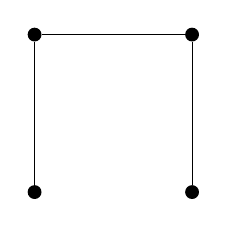
\begin{tikzpicture}[baseline={([yshift=-.5ex]current bounding box.center)}]
                \node[fill, circle, inner sep = 0, minimum size = 5pt] at (0, 0) (1) {};
                \node[fill, circle, inner sep = 0, minimum size = 5pt] at (2, 0) (2) {};
                \node[fill, circle, inner sep = 0, minimum size = 5pt] at (0, -2) (3) {};
                \node[fill, circle, inner sep = 0, minimum size = 5pt] at (2, -2) (4) {};
                \draw (1) -- (2);
                \draw (1) -- (3);
                \draw (2) -- (4);
            \end{tikzpicture}
        \end{gather*}
        Higher powers of a given coordinate would then, for example, give rise to diagrams with loops at a given vertex:
        \begin{gather*}
            A^{-1}_{11}A^{-1}_{12}A^{-1}_{22} =
            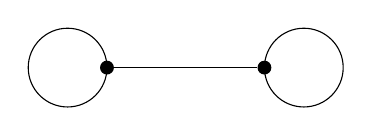
\begin{tikzpicture}[baseline={([yshift=-.5ex]current bounding box.center)}]
                \node[fill, circle, inner sep = 0, minimum size = 5pt] at (0, 0) (1) {};
                \node[fill, circle, inner sep = 0, minimum size = 5pt] at (2, 0) (2) {};
                \draw (-0.5, 0) circle (0.5);
                \draw (1) -- (2);
                \draw (2.5, 0) circle (0.5);
            \end{tikzpicture}
        \end{gather*}
    \end{example}

    \begin{remark}[Normalization]
        In practice, one often divides all Gaussian integrals by the quantity $I(A,0)$ to cancel the normalization factor. In the functional setting, this is even imperative since, as mentioned above, the normalization factor diverges for infinite-dimensional spaces.
    \end{remark}

\subsection{Generalizations}

    \newdef{Henstock--Kurzweil integral\footnotemark}{\index{integral!Henstock--Kurzweil}\index{integral!Perron}\index{integral!Denjoy}\index{integral!Luzin}\index{gauge|seealso{integral, Denjoy}}\index{integral!McShane}
    \footnotetext{Also called the \textbf{Perron}, \textbf{Lusin}, \textbf{(narrow) Denjoy} or \textbf{gauge} integral.}
        Consider the usual definition of the (proper) Riemann integral, where tagged partitions $P$ of $[a,b]$ are chosen and the integral is obtained as the limit of the Riemann sums
        \begin{gather}
            I = \sum_Pf(x_i)(t_i-t_{i-1})
        \end{gather}
        as the mesh size of the partitions goes to zero.

        Now, to obtain the generalized integral, consider a strictly positive function $\delta:[a,b]\mathbb{R}^{>0}$, the \textbf{gauge function}. Given such a gauge, a tagged partition $P$ is said to be \textbf{$\delta$-fine} if
        \begin{gather}
            [t_{i-1},t_i]\subset[x_i-\delta(x_i),x_i+\delta(x_i)]
        \end{gather}
        for subintervals in the partition.\footnote{If the condition $x_i\in[t_{i-1},t_i]$ in the definition of tagged partitions is dropped, the \textbf{McShane integral} is obtained. This can be shown to be equivalent to the \textit{Lebesgue integral} (see \cref{chapter:measure}).}

        If the integral exists, it is given by the number $I\in\mathbb{R}$ such that for all $\varepsilon>0$ there exists a gauge $\delta:[a,b]\rightarrow\mathbb{R}^{>0}$ such that, if $P$ is $\delta$-fine, then
        \begin{gather}
            \left\vert I-\sum_Pf(x_i)(t_i-t_{i-1})\right\vert<\varepsilon\,.
        \end{gather}
    }
    \begin{remark}[Riemann integral]\index{integral!Riemann}
        If the gauge functions are chosen to be constant, the classical $(\varepsilon,\delta)$-definition of ordinary Riemann integrals is obtained.
    \end{remark}

    The following statement can be seen as a refinement of \cref{topology:heine_borel}. Moreover, it is also sometimes known as the \textbf{Borel--Lebesgue theorem}.\index{Borel--Lebesgue}
    \begin{property}[Cousin]\index{Cousin}
        For every gauge $\delta:[a,b]\rightarrow\mathbb{R}^{>0}$, there exists a $\delta$-fine partition. 
    \end{property}

    \begin{property}[Integrability]
        If $f:[a,b]\rightarrow\mathbb{R}$ is bounded, then the following are equivalent:
        \begin{itemize}
            \item $f$ is Henstock--Kurzweil integrable, and
            \item $f$ is \textit{Lebesgue integrable} (see \cref{chapter:measure}).
        \end{itemize}
        More generally, a function $f:[a,b]\rightarrow\mathbb{R}$ is Henstock--Kurzweil integrable if and only if both $f$ and $|f|$ are \textit{Lebesgue integrable}.
    \end{property}

    The following property shows that `improper' Henstock--Kurzweil integrals are only truly improper for unbounded domains.
    \begin{property}[Hake]\index{Hake}
        \begin{gather}
            \Int_a^bf\,dx = \lim_{c\nearrow b}\Int_a^cf\,dx\,,
        \end{gather}
        whenever either side exists.
    \end{property}

    One of the most important arguments for using the Henstock--Kurzweil integral is its refinement of the Second Fundamental Theorem of Calculus~\ref{calculus:second_fundamental_theorem}. Note that the theorem for the Riemann integral required that the derivative was integrable. The gauge integral relaxes this condition.
    \begin{theorem}[Second fundamental theorem of calculus]
        Let $f:[a,b]\rightarrow\mathbb{R}$ be differentiable, then
        \begin{gather}
            \Int_a^xf'(x')\,dx' = f(x)-f(a)\text{\ \ a.e.}
        \end{gather}
    \end{theorem}

\section{Convexity}

    \newdef{Convex set}{\index{convex}\index{hull}\label{calculus:convex}
        A subset of $X$ of a vector space $V$ (\cref{linalgebra:vector_space}) is said to be convex if $x,y\in X$ implies that $\bigl\{\lambda x+(1-\lambda)y\mid\lambda\in[0,1]\bigr\}\subset X$, i.e.~if all straight lines connecting elements of the set are completely contained in that set. The \textbf{convex hull} of a subset $X$ is defined as the smallest convex subset containing $X$.
    }

    \newdef{Extreme point}{\index{extreme!point}\label{calculus:extreme_point}
        Consider a convex set $X$. The extreme points of $X$ are the points $p\in X$ such that, if
        \begin{gather}
            p = \lambda p_1 + (1-\lambda)p_2
        \end{gather}
        for some $p_1,p_2\in X$ and $\lambda\in[0,1]$, then $p_1=p_2=p$.
    }

    \newdef{Convex function}{\label{calculus:convex_function}
        Let $X$ be a convex set. A function $f:X\rightarrow\mathbb{R}$ is said to be convex if for all $x,y\in X$ and $\lambda\in[0,1]$:
        \begin{gather}
            f\bigl(\lambda x + (1-\lambda)y\bigr)\leq t\lambda(x) + (1-\lambda)f(y)\,.
        \end{gather}
        For the definition of a \textbf{concave} function, the inequality has to be turned around.
    }
    \newdef{Linear map}{\index{linear!map}
        A function $f:X\rightarrow\mathbb{R}$ is linear if and only if it is both convex and concave.
    }

    \begin{theorem}[Karamata's inequality]\index{Karamata}
        Consider an interval $I\subset\mathbb{R}$ and let $f:I\rightarrow\mathbb{R}$ be a convex function. If $(x_1,\ldots,x_n)$ is a tuple that majorizes $(y_1,\ldots,y_n)$, i.e.
        \begin{gather}
            \sum_{i=1}^nx_i = \sum_{i=1}^ny_i
        \end{gather}
        and
        \begin{gather}
            x_{(1)} + \cdots + x_{(k)}\geq y_{(1)} + \cdots + y_{(k)}
        \end{gather}
        for all $k\leq n$, where $x_{(i)}$ denotes the $i^{\text{th}}$ largest element of $(x_1,\ldots,x_n)$, then
        \begin{gather}
            \sum_{i=1}^nf(x_i)\geq\sum_{i=1}^nf(y_i)\,.
        \end{gather}
    \end{theorem}

    The following inequality can be derived directly from the definition of convexity by induction.
    \begin{theorem}[Jensen's inequality]\index{Jensen's inequality}\label{calculus:jensen_inequality}
        Let $f$ be a convex function and consider a point $\{a_i\}_{i\leq n}$ in the probability simplex $\Delta^n$ (\cref{topology:standard_simplex}).
        \begin{gather}
            f\left(\sum_{i=1}^na_ix_i\right)\leq\sum_{i=1}^na_if(x_i)\,.
        \end{gather}
    \end{theorem}

    \newdef{Legendre transformation}{\index{Legendre!transformation}\label{calculus:legendre}
        Consider a function $f:\mathbb{R}\rightarrow\mathbb{R}$. In certain cases (especially in physics) it is sometimes useful to replace the argument $x$ by the slope of $f$ at $x$, i.e.~to perform the transformation
        \begin{gather}
            x\longrightarrow f'(x)\,.
        \end{gather}
        However, it should be clear that this transformation is not always well-defined and, even if it is, it does not always preserve all the information contained in $f$.

        These conditions are satisfied exactly if $f$ is convex (or concave). In this case, the Legendre transform of $f$ is defined as
        \begin{gather}
            f^*(x^*) := \sup_x\bigl(x^*x - f(x)\bigr)\,.
        \end{gather}
        Now, consider the case where $f$ is differentiable. The above supremum can then be obtained by differentiating the right-hand side and equating it to zero. This results in $x^* = f'(x)$, which is exactly the transformation that was required. By expressing everything in terms of the Legendre tranformed quantity $x^*$, one can also find the derivative of $f^*$:
        \begin{gather}
            \deriv{f^*}{x^*}(x^*) = x(x^*)\,.
        \end{gather}
    }

    \begin{property}[Alternative characterization]\label{calculus:legendre_condition}
        In fact, up to an additive constant, the condition
        \begin{gather}
            (f^*)' = (f')^{-1}
        \end{gather}
        uniquely determines the Legendre transformation.
    \end{property}
    \begin{remark}
        These definitions can easily be extended to higher dimensions ($n\geq2$).
    \end{remark}

\section{Trigonometry}

    \newdef{Trigonometric functions}{\index{sine}\index{cosine}\index{tangent}
        Consider \cref{fig:right_triangle}. In a right(-angled) triangle, the trigonometric functions of the angle $\theta$ are defined as follows:
        \begin{gather}
                \sin(\theta) := \frac{y}{x}\qquad\qquad
                \cos{\theta} := \frac{z}{x}\qquad\qquad
                \tan(\theta) := \frac{y}{z}
        \end{gather}
    }
    \begin{result}
        \begin{gather}
            \tan(\theta) = \frac{\sin(\theta)}{\cos(\theta)}
        \end{gather}
    \end{result}

    \begin{figure}[ht!]
        \centering
        \begin{tikzpicture}
            \draw (0, 0) node[below left]{$A$} -- node[left]{$z$} (0, 2) node[above left]{$B$} node[below = .5cm, right = .1cm]{$\theta$} -- node[above right]{$x$} (5, 0) node[below right]{$C$} -- node[below]{$y$} (0, 0);
        \end{tikzpicture}
        \caption{Right(-angled) triangle.}
        \label{fig:right_triangle}
    \end{figure}
% \chapter{Complex Analysis}\label{chapter:complexcalculus}

\section{Complex algebra}

    The set of complex numbers $\mathbb{C}$ forms a 2-dimensional vector space over the field of real numbers (\cref{chapter:linear_algebra}). At the same time, the operations of complex addition and complex multiplication also turn the complex numbers into a field.

    \newdef{Complex conjugate}{\index{complex conjugate}
        Complex conjugation
        \begin{gather}
            \overline{\,\cdot\,\vphantom{z}}:a+bi\mapsto a-bi
        \end{gather}
        is an involution (\cref{set:involution}). It is sometimes denoted by $z^*$ instead of $\overline{z}$, but, unless this would cause confusion, the former notation will be used throughout this compendium.
    }

    \newformula{Real/imaginary part}{
        A complex number can also be written as
        \begin{gather}
            \mathrm{Re}(z) + i\ \mathrm{Im}(z)\,,
        \end{gather}
        where
        \begin{align}
            \mathrm{Re}(z) &:= \frac{z + \overline{z}}{2}\,,\\
            \mathrm{Im}(z) &:= \frac{z - \overline{z}}{2i}\,.
        \end{align}
    }
    \newdef{Argument}{\index{argument}\index{polar!form}
        Consider a complex number expressed in \textit{polar form}:
        \begin{gather}
            z = re^{i\theta}
        \end{gather}
        The number $\theta$ is called the argument of $z$ and it is denoted by $\arg(z)$.

        \todo{DERIVE POLAR FORM}
    }

    \newdef{Riemann sphere}{\index{Riemann!sphere}
        Consider the one-point compactification $\overline{\mathbb{C}} = \mathbb{C}\cup\{\infty\}$ (\cref{topology:alexandrov_compactification}). This set is called the Riemann sphere or \textbf{extended complex plane}. The standard operations on $\mathbb{C}$ can be generalized to $\overline{\mathbb{C}}$ for all nonzero $z\in\mathbb{C}$ in the following way:
        \begin{align}
            z + \infty &:= \infty\nonumber\\
            z * \infty &:= \infty\\
            \frac{z}{\infty} &:= 0\,.\nonumber
        \end{align}
        Since there exists no multiplicative inverse for $\infty$, the Riemann sphere is not a field.
    }

\section{Holomorphic functions}

    \newdef{Holomorphic function}{\index{holomorphic!function}\label{complexcalculus:holomorphic}
        A function $f$ on an open set $U\subseteq\mathbb{C}$ that is complex differentiable at every point $z_0\in U$, i.e.~for every point $z_0\in U$ the following limit exists:
        \begin{gather}
            f'(z_0) := \lim_{z\rightarrow z_0}\frac{f(z) - f(z_0)}{z-z_0}\,.
        \end{gather}
    }
    \newdef{Biholomorphic function}{\index{bi-!holomorphic}
        A holomorphic function admitting a holomorphic inverse.
    }
    \newdef{Entire}{\index{entire}
        A function that is holomorphic on all of $\mathbb{C}$.
    }

    \begin{property}[Cauchy--Riemann conditions]\index{Cauchy--Riemann!conditions}\label{complex:cauchy_riemann}\index{Wirtinger derivative}
        A holomorphic function $f$ satisfies the following conditions:
        \begin{gather}
            \pderiv{u}{x} = \pderiv{v}{y} \text{\qquad and\qquad} \pderiv{u}{y} = -\pderiv{v}{x}\,.
        \end{gather}
        These conditions can be combined into one equation using the so-called \textbf{Wirtinger derivative}:
        \begin{gather}
            \label{complex:holomorphic_alternative_condition}
            \pderiv{f}{\overline{z}} = 0\,.
        \end{gather}
    \end{property}

    \begin{theorem}[Looman--Menchoff\footnotemark]\index{Looman--Menchoff}\index{Cauchy--Goursat|see{Looman--Menchoff}}
        \footnotetext{This is the most general theorem on the holomorphy of continuous functions. It generalizes the original results by \textit{Riemann} and \textit{Cauchy--Goursat}.}
        Let $f$ be a continuous function defined on a subset $U\in\mathbb{C}$. If the partial derivatives of the real and imaginary part exist and if $f$ satisfies the Cauchy--Riemann conditions, then $f$ is holomorphic on $U$.
    \end{theorem}

    \begin{property}[Laplace equation]\index{harmonic!function}
        The functions $u,v$ satisfying the Cauchy--Riemann conditions are harmonic functions, i.e.~they satisfy the \textit{Laplace equation} (see \cref{pde:laplace_equation}).
    \end{property}
    \begin{property}[Level sets]
        The functions $u,v$ satisfying the Cauchy--Riemann conditions have orthogonal level curves (\cref{set:level_set}).
    \end{property}

    \begin{property}[Real functions]
        Consider a real-valued function $f$ defined on the complex plane. If it is holomorphic, the Cauchy--Riemann conditions imply that $f$ is a constant.
    \end{property}

    \begin{theorem}[Identity theorem]\index{identity!theorem}
        If two holomorphic functions on a domain $D$ coincide on a set containing an accumulation point of $D$, they coincide on all of $D$.
    \end{theorem}

\section{Contour integrals}

    \sremark{Whenever contours are considered for integration purposes, they have been chosen to be evaluated counter-clockwise (by convention). To obtain results concerning clockwise evaluation, most of the time adding a minus sign is sufficient.}

    \newdef{Contour integral}{\index{integral!contour}\label{complex:contour_integral}
        The contour integral of a complex function
        \begin{gather}
            f(z)=u(z)+iv(z)
        \end{gather}
        is defined as the following line integral:
        \begin{gather}
            \Int_{z_1}^{z_2}f(z)\,dz = \Int_{(x_1,y_1)}^{(x_2,y_2)}\bigl(u(x,y) + iv(x,y)\bigr)(dx+idy)\,.
        \end{gather}
    }

    \begin{theorem}[Cauchy's integral theorem\footnotemark]\index{Cauchy!integral theorem}\index{rectifiable curve}\index{Cauchy--Goursat}\label{complex:cauchy_integral_theorem}
        \footnotetext{Also called the \textbf{Cauchy--Goursat theorem}.}
        Let $\Omega$ be a simply-connected subset of $\mathbb{C}$ and let $f:\mathbb{C}\rightarrow\mathbb{C}$ be a holomorphic function on $\Omega$. The contour integral around every closed, rectifiable (i.e.~of finite length) contour $C$ in $\Omega$ vanishes:
        \begin{gather}
            \Oint_Cf(z)\,dz = 0\,.
        \end{gather}
    \end{theorem}
    \begin{result}[Freedom of contour]
        The contour integral of a holomorphic function depends only on the limits of integration and not on the contour connecting them.
    \end{result}

    \begin{formula}[Cauchy's integral formula]\index{Cauchy!integral formula}\label{complex:cauchy_integral_formula}
        Let $\Omega$ be a connected subset of $\mathbb{C}$ and let $C$ be a closed contour in $\Omega$. If $f:\mathbb{C}\rightarrow\mathbb{C}$ is holomorphic on $\Omega$, then, at every point $z_0$ inside $C$, one can express $f$ as follows:
        \begin{gather}
            f(z_0) = \frac{1}{2\pi i}\Oint_C\,\frac{f(z)}{z-z_0}\,dz\,.
        \end{gather}
    \end{formula}

    \begin{result}[Analytic function]\index{analytic!function}\label{complex:cauchy_integral_formula_derivative}
        Let $\Omega$ be a connected subset of $\mathbb{C}$ and let $C$ be a closed contour in $\Omega$. If $f:\mathbb{C}\rightarrow\mathbb{C}$ is holomorphic on $\Omega$, then $f$ is analytic (\cref{calculus:analytic}) on $\Omega$ and
        \begin{gather}
            f^{(n)}(z_0) = \frac{1}{2\pi i}\Oint_Cf(z)\frac{n!}{(z-z_0)^{n+1}}\,dz\,.
        \end{gather}
        Furthermore, the derivatives are also holomorphic on $\Omega$.
    \end{result}

    \begin{theorem}[Morera]\index{Morera}
        If $f:\mathbb{C}\rightarrow\mathbb{C}$ is continuous on a connected open set $\Omega$ and
        \begin{gather}
            \Oint_Cf(z)\,dz=0
        \end{gather}
        for every closed contour $C$ in $\Omega$, then $f$ is holomorphic on $\Omega$.
    \end{theorem}

    \begin{theorem}[Liouville]\index{Liouville!theorem on entire functions}
        Every bounded, entire function is constant.
    \end{theorem}

    \begin{theorem}[Sokhotski--Plemelj]\index{Sokhotski--Plemelj}\label{complex:sokhotski_plemelj}
        Let $f:\mathbb{R}\rightarrow\mathbb{C}$ be continuous and consider $a<0<b$, then
        \begin{gather}
            \lim_{\varepsilon\rightarrow0^+}\Int_a^b\frac{f(x)}{x\pm i\varepsilon}\,dx = \mp i\pi f(0) + \mathcal{P}\Int_a^b\frac{f(x)}{x}\,dx\,,
        \end{gather}
        where $\mathcal{P}$ denotes the Cauchy principal value.

        \todo{ADD (Cauchy principal value)}
    \end{theorem}

\section{Laurent series}

    \begin{definition}[Laurent series]\index{Laurent!series}\index{annulus}\index{principal!part}\label{complex:laurent_series}
        If $f:\mathbb{C}\rightarrow\mathbb{C}$ is an analytic function defined on an \textbf{annulus}, i.e.~a ring-shaped region, then $f$ can be expanded as the following series:
        \begin{gather}
            f(z) = \sum^{+\infty}_{n=-\infty}a_n(z-z_0)^n \qquad\text{with}\qquad a_n = \frac{1}{2\pi i}\Oint\frac{f(z)}{(z-z_0)^{n+1}}\,dz\,.
        \end{gather}
        The subseries containing all terms of negative degree is called the \textbf{principal part} of the Laurent series. 
    \end{definition}
    \begin{notation}
        The ring of Laurent series in the indeterminate $z$ is given by the ring $\mathbb{C}[[z,z^{-1}]]$. Therefore, it is also sometimes denoted by $\mathbb{C}((z))$.
    \end{notation}

    \begin{property}[Convergence]
        The Laurent series of an analytic function $f:\mathbb{C}\rightarrow\mathbb{C}$ converges uniformly to $f$ on the annulus $R_1 < |z-z_0| < R_2$, with $R_1$ and $R_2$ the distances from $z_0$ to the two closest \textit{poles} (see \cref{complex:pole} further below).
    \end{property}

    \newdef{Analytic continuation}{\index{analytic!continuation}
        Consider an analytic function $f:\mathbb{C}\rightarrow\mathbb{C}$ defined on an open subset $U\subset\mathbb{C}$. If $V\subset\mathbb{C}$ is an open subset containing $U$ and if there exists an analytic function $F$ on $V$ such that $F(z)=f(z)$ for all $z\in U$, then $F$ is called the analytic continuation of $f$ to $V$. Using the identity theorem for holomorphic functions, one can prove that analytic continuations are unique (on connected domains).
    }

    \begin{theorem}[Schwarz's reflection principle]\index{Schwarz!reflection principle}
        Let $f:\mathbb{C}\rightarrow\mathbb{C}$ be analytic on the upper half plane. If $z\in\mathbb{R}\implies f(z)\in\mathbb{R}$, then
        \begin{gather}
            f\bigl(\overline{z}\bigr) = \overline{f(z)}\,.
        \end{gather}
    \end{theorem}

\section{Singularities}
\subsection{Poles}

    \newdef{Pole}{\index{pole}\label{complex:pole}
        A function $f:\mathbb{C}\rightarrow\mathbb{C}$ has a pole of order $m\in\mathbb{N}_0$ at a point $z_0\in\mathbb{C}$ if its Laurent series at $z_0$ satisfies $\forall n<-m:a_n = 0$ and $a_{-m}\neq0$.
    }

    \newdef{Meromorphic}{\index{meromorphic}
        A function $f:\mathbb{C}\rightarrow\mathbb{C}$ is said to be meromorphic if it is analytic on the whole complex plane with exception of isolated poles and removable singularities. Every meromorphic function can be written as a fraction of two holomorphic functions, where the poles coincide with the zeros of the denominator.
    }

    \newdef{Essential singularity}{\index{essential!singularity}
        A function $f$ has an essential singularity at a point $z_0$ if its Laurent series at $z_0$ satisfies $\forall n\in\mathbb{N}:a_{-n}\neq0$, i.e.~if its Laurent series has infinitely many negative degree terms.
    }

    \newmethod{Frobenius transformation}{\index{Frobenius!transformation}
        To study the behaviour of a function $f$ at $z\longrightarrow\infty$, one can apply the Frobenius transformation $h=1/z$ and study the limit $\lim_{h\rightarrow0}f(h)$. For example, a singularity at $\infty$ is defined as a singularity of $f(1/z)$ at 0.
    }
    \begin{property}[Polynomials]\index{poly-!nomial}
        An entire function $f:\mathbb{C}\rightarrow\mathbb{C}$ is polynomial if and only if it has a pole at $\infty$.
    \end{property}

    \begin{theorem}[Casorati--Weierstrass]\index{Casorati--Weierstrass}
        Let $f:\mathbb{C}\rightarrow\mathbb{C}$ be holomorphic on the punctured open set $U\backslash\{z_0\}$ with an essential singularity at $z_0$. For every neighbourhood $V$ of $z_0$ contained in $U$, the image $f(V\backslash\{z_0\})$ is dense in $\mathbb{C}$.
    \end{theorem}
    \begin{result}
        If $f:\mathbb{C}\rightarrow\mathbb{C}$ is a nonpolynomial, entire function, then, for every $c\in\mathbb{C}$, there exists a sequence $z_n\longrightarrow\infty$ such that $f(z_n)\longrightarrow c$.\footnote{Polynomials are excluded due to the property above.}
    \end{result}

    \begin{theorem}[Picard's little theorem]\index{Picard}
        The range of a nonconstant, entire function is the complex plane with at most a single exception.
    \end{theorem}
    \begin{theorem}[Picard's great theorem]
        Let $f:\mathbb{C}\rightarrow\mathbb{C}$ be an analytic function with an essential singularity at $z_0$. On every punctured neighbourhood of $z_0$, $f$ takes on all possible values, with at most a single exception, infinitely many times.
    \end{theorem}

\subsection{Branch cuts}

    \newformula{Roots}{\index{root}
        Let $z\in\mathbb{C}$. The $n^{\text{th}}$ roots\footnote{Also see the fundamental theorem of algebra (\cref{alggeom:fundamental_theorem_of_algebra}).} of $z = re^{i\theta}$ are given by
        \begin{gather}
            \left\{\sqrt[n]{r}\exp\left(\frac{\theta + 2\pi k}{n}i\right)\,\middle\vert\,k\in\{0,1,\ldots,n\}\right\}\,.
        \end{gather}
    }
    \newformula{Complex logarithm}{\index{logarithm}
        The natural logarithm can be continued to the complex plane (as a multi-valued function) as follows:
        \begin{gather}
            \mathrm{LN}(z) := \bigl\{\ln(r) + i(\theta + 2\pi k)\bigm\vert k\in\mathbb{Z}\bigr\}\,.
        \end{gather}
    }

    \newdef{Branch}{\index{branch}
        The problem with the previous two formulas is that they represent multi-valued functions. To get an unambiguous image it is necessary to fix a value of the parameter $k$. By doing so there will arise curves, called \textbf{branch cuts}, in the complex plane where the function becomes discontinuous. A \textbf{branch} is defined as a particular choice of the parameter $k$.

        For the logarithm, the choice for $\arg(\mathrm{LN})\in\ ]\alpha, \alpha + 2\pi]$ is often denoted by $\mathrm{LN}_\alpha$ or $\log_\alpha$.
    }
    \newdef{Principal value}{\index{principal!value}
        The principal value\footnote{Not to be confused with the Cauchy principal value.} of a multi-valued complex function is defined as the value associated with a choice of branch for which $\arg(f)\in\ ]\!-\pi,\pi]$.
    }

    \newdef{Branch point}{
        Let $f$ be a complex-valued function. A point $z_0$ for which there exists no neighbourhood on which $f$ is single-valued is called a branch point.
    }
    \newdef{Branch cut}{
        A line connecting exactly two branch points, one possibly being $\infty$, is called a branch cut. In case there exist multiple branch cuts, they are required to never cross.
    }

    \begin{example}
        Consider the complex function
        \begin{gather}
            f(z) = \frac{1}{\sqrt{(z-z_1)\cdots(z-z_n)}}\,.
        \end{gather}
        This function has singularities at $z_1,\ldots,z_n$. If $n$ is even, this function will have $n$ (finite) branch points. This implies that the points can be grouped in pairs connected by non-intersecting branch cuts. If $n$ is odd, this function will have $n$ (finite) branch points and one branch point at infinity. The finite branch points will be grouped in pairs connected by non-intersecting branch cuts and the remaining branch point will be joined to infinity by a branch cut that does not intersect the others.
    \end{example}

\subsection{Residue theorem}\index{residue}

    \newdef{Residue}{\label{complex:residue_def}
        By applying \cref{complex:contour_integral} to a polynomial function, one finds
        \begin{gather}
            \Oint_C(z-z_0)^n\,dz = 2\pi i\delta_{n,-1}\,,
        \end{gather}
        where $C$ is a contour around the pole $z=z_0$. This means that integrating a Laurent series around a pole isolates the coefficient $a_{-1}$. This coefficient is, therefore, called the residue of the function at the given pole.
    }
    \begin{notation}
        The residue of a complex function $f:\mathbb{C}\rightarrow\mathbb{C}$ at a pole $z_0$ is denoted by
        \begin{gather}
            \mathrm{Res}[f(z)]_{z=z_0}\,.
        \end{gather}
    \end{notation}

    \begin{formula}
        For a pole of order $m\in\mathbb{N}_0$, the residue is calculated as follows:
        \begin{gather}
            \label{complex:residue}
            \mathrm{Res}\left[f(z)\right]_{z=z_j} = \lim_{z\rightarrow z_0}\frac{1}{(m - 1)!} \left(\pderiv{}{z}\right)^{m-1}\left(f(z)(z-z_0)\right)\,.
        \end{gather}
        For essential singularities, the residue can be found by writing out the Laurent series explicitly.
    \end{formula}

    \begin{theorem}[Residue theorem]\label{complex:residue_theorem}
        If $f:\mathbb{C}\rightarrow\mathbb{C}$ is meromorphic on $\Omega\subseteq\mathbb{C}$ and if $C$ is a closed contour in $\Omega$ that contains the poles $z_j$ of $f$, then
        \begin{gather}
            \Oint_Cf(z)\,dz = 2\pi i\sum_j\mathrm{Res}\left[f(z)\right]_{z=z_j}\,.
        \end{gather}
        For poles on the contour $C$, only half of the residue contributes to the integral.
    \end{theorem}

    \begin{formula}[Argument principle]\index{argument!principle}
        Let $f:\mathbb{C}\rightarrow\mathbb{C}$ be meromorphic and denote the number of zeros and poles of $f$ inside the contour $C$ by $Z_f(C)$ and $P_f(C)$, respectively. From the residue theorem, one can derive the following formula:
        \begin{gather}
            \frac{1}{2\pi i}\Oint_C\frac{f(z)}{f'(z)}\,dz = Z_f(C) - P_f(C)\,.
        \end{gather}
    \end{formula}
    \begin{definition}[Winding number]\index{winding number}\index{index!of map}
        Let $f:\mathbb{C}\rightarrow\mathbb{C}$ be meromorphic and let $C$ be a simple closed contour. For all $a\not\in f(C)$, the winding number, also called the \textbf{index}, of $a$ with respect to the function $f$ is defined as follows:
        \begin{gather}
            \mathrm{Ind}_f(a) := \frac{1}{2\pi i}\Oint_C\frac{f'(z)}{f(z) - a}\,dz\,.
        \end{gather}
        This number is always an integer.
    \end{definition}

\section{Limit theorems}

    \begin{theorem}[Small limit theorem]\index{limit!theorem}\label{complex:small_limit}
        Let $f:\mathbb{C}\rightarrow\mathbb{C}$ be a function that is holomorphic almost everywhere and let the contour $C$ be a circular segment with radius $\varepsilon$ and central angle $\alpha$. If $z$ is parametrized as $z=\varepsilon e^{i\theta}$, then
        \begin{gather}
            \Oint_Cf(z)\,dz = i\alpha A
        \end{gather}
        with
        \begin{gather}
            A = \lim_{\varepsilon\rightarrow0}f(z)\,\,.
        \end{gather}
    \end{theorem}

    \begin{theorem}[Great limit theorem]\label{complex:great_limit}
        Let $f:\mathbb{C}\rightarrow\mathbb{C}$ be a function that is holomorphic almost everywhere and let the contour $C$ be a circular segment with radius $R$ and central angle $\alpha$. If $z$ is parametrized as $z=Re^{i\theta}$, then
        \begin{gather}
            \Oint_Cf(z)\,dz = i\alpha B
        \end{gather}
        with
        \begin{gather}
            B = \lim_{R\rightarrow\infty}f(z)\,.
        \end{gather}
    \end{theorem}

    \begin{theorem}[Jordan's lemma]\index{Jordan}\label{complex:jordan}
        Let $g:\mathbb{C}\rightarrow\mathbb{C}$ be a continuous function that can be written as $g(z) = f(z)e^{bz}$ and let the contour $C$ be a semicircle lying in the half-plane bounded by the real axis and oriented away of the point $i\overline{b}$. If $z$ is parametrized as $z=Re^{i\theta}$ and
        \begin{gather}
            \lim_{R\rightarrow\infty}f(z) = 0\,,
        \end{gather}
        then
        \begin{gather}
            \Oint_Cg(z)\,dz = 0\,.
        \end{gather}
    \end{theorem}
% \chapter{Measure \& Integration Theory}\label{chapter:measure}

    The main references for this chapter are~\citet{capinski_measure_2013,choquet-bruhat_analysis_1991}.

    \minitoc

\section{Measure theory}
\subsection{General definitions}

    \newdef{Measure}{\index{measure}\index{outer!measure}\index{$\sigma$!additivity}\label{measure:measure}
        Recall \cref{set:sigma_algebra} and consider a measurable space $(X,\Sigma)$. A function $\mu:\Sigma\rightarrow\overline{\mathbb{R}}$ is called a measure if it satisfies the following conditions:
        \begin{enumerate}
            \item\textbf{Nonnegativity}: $\forall E\in\Sigma:\mu(E)\geq0$,
            \item\textbf{Empty set is null}: $\mu(\emptyset)=0$, and
            \item\textbf{$\sigma$-additivity}: $\forall i\neq j:E_i\cap E_j=\emptyset\implies\mu\left(\bigcup_{n=1}^\infty E_n\right) = \sum_{i=n}^{+\infty}\mu(E_n)$.
        \end{enumerate}
        When $\mu$ is defined on all of $P(X)$ and only satisfies countable subadditivity, i.e.~the equality in the last condition becomes an inequality $\leq$, it is called an \textbf{outer measure}.
    }
    \begin{remark}
        To show that two measures coincide on a $\sigma$-algebra, it suffices to show that they coincide on the generating sets and apply the Monotone Class Theorem~\ref{set:monotone_class}.
    \end{remark}

    \newdef{Measure space}{\label{measure:measure_space}
        A triple $(X,\Sigma,\mu)$, where the pair $(X,\Sigma)$ is a measurable space and $\mu$ is a measure thereon, is called a measure space.
    }

    \newdef{Null set}{\index{null!set}
        A set $A\subset\mathbb{R}$ is said to be null if $\mu(A)=0$.
    }

    \newdef{Almost everywhere\footnotemark}{\index{almost everywhere}\label{measure:almost_everywhere}
        \footnotetext{In probability theory this is often called \textbf{almost surely}.}
        Let $(X,\Sigma,\mu)$ be a measure space. A property $P$ is said to hold on $X$ almost everywhere (abbreviated as \textbf{a.e.}) if it satisfies the following equation:
        \begin{gather}
            \mu\bigl(\{x\in X\bigm\vert\neg P(x)\}\bigr) = 0\,,
        \end{gather}
        i.e.~it holds everywhere except for a null set.
    }

    \newdef{Complete measure space}{\index{complete!measure space}
        A measure space $(X,\Sigma,\mu)$ is said to be complete if for every $E\in\Sigma$ with $\mu(E)=0$ the implication $A\subset E\implies A\in\Sigma$ holds. Additivity then necessarily implies that $\mu(A)=0$.
    }
    \newdef{Completion}{
        Let $\Sigma\subseteq\overline{\Sigma}$ be $\sigma$-algebras on a set $X$. $(X,\overline{\Sigma},\overline{\mu})$ is called the completion of $(X,\Sigma,\mu)$ if:
        \begin{enumerate}
            \item $\forall A\in\Sigma:\overline{\mu}(A)=\mu(A)$,
            \item $(X,\overline{\Sigma},\overline{\mu})$ is complete, and
            \item $\overline{\Sigma}$ is the smallest $\sigma$-algebra with these properties.
        \end{enumerate}
    }

    \newdef{\texorpdfstring{$\sigma$-}{sigma-}finite measure}{\index{$\sigma$!finite}\label{measure:sigma_finite_measure}
        Let $(X,\Sigma,\mu)$ be a measure space. The measure $\mu$ is said to be $\sigma$-finite if there exists a sequence $\seq{A}$ of measurable sets such that $\bigcup_{n=1}^{+\infty}A_n=X$ with $\forall n\in\mathbb{N}:\mu(A_n)<+\infty$.
    }

    \newdef{Borel measure}{\index{Borel!measure}
        Consider a topological space together with its Borel $\sigma$-algebra (\cref{topology:borel_set}). Any measure defined on this measurable space is called a Borel measure.
    }

    \newdef{Locally finite measure}{
        A measure on a Hausdorff space whose measurable sets contain the Borel sets such that every point has an open neighbourhood of finite measure. On locally compact spaces, this is equivalent to requiring that every compact subset has finite measure.
    }

    Given a Borel measure on a topological space, there are different ways of how one can approximate the measure of Borel sets by those of open or closed sets. Sadly, different distinct definitions can be found in the literature all under the name of `regular' measure. The next definition gives the most widely used ones.
    \newdef{Regular measure}{\label{measure:regular_measure}
        An outer measure $\mu$ on a topological space $X$ whose completion contains the Borel sets is said to be \textbf{Borel regular} if for every set $A\subset X$, there exists a Borel set $B\subseteq A$ such that $\mu(A)=\mu(B)$.

        Let $\mu$ be a measure on $(X,\Sigma)$, where $X$ is a topological space. It is said to be \textbf{regular} if if it satisfies the following conditions for every measurable set $B$:
        \begin{enumerate}
            \item\textbf{Outer regularity}: $\mu(B)=\inf\bigl\{\mu(O)\bigm\vert O\text{ open and measurable},O\supset B\bigr\}$, and
            \item\textbf{Inner regularity}: $\mu(B)=\sup\bigl\{\mu(K)\bigm\vert K\text{ closed and measurable},K\subset B\bigr\}$.
        \end{enumerate}
        If $X$ is Hausdorff, the measure is said to be \textbf{regular} if it satisfies the following conditions for every measurable set $B$:
        \begin{enumerate}
            \item\textbf{Outer regularity}: $\mu(B)=\inf\bigl\{\mu(O)\bigm\vert O\text{ open and measurable},O\supset B\bigr\}$, and
            \item\textbf{Inner regularity} or \textbf{tightness}: $\mu(B)=\sup\bigl\{\mu(K)\bigm\vert K\text{ compact and measurable},K\subset B\bigr\}$.
        \end{enumerate}
        Note that since compact subsets of Hausdorff spaces are closed, tight measures are in particular regular.
    }

    By slightly modifying the definition of tight Borel measures, one can obtain yet another type of regularity.
    \newdef{Radon measure}{\index{Radon!measure}\index{locally!finite}\label{measure:radon_measure}
        A Borel measure on a Hausdorff space that is outer regular on Borel sets, inner regular on open sets and locally finite. (For locally compact spaces, outer regularity is superfluous.)
    }

    \newdef{Radon space}{\index{Radon!space}
        A topological space on which every finite Borel measure is Radon. It is sometimes called \textbf{strongly Radon} if every locally finite Borel measure is Radon.
    }
    \begin{example}
        Locally compact, separable metric space, Polish spaces and even Suslin spaces (\cref{metric:suslin}) are Radon. Slightly weaker, every finite Borel measure on a metric space is regular.
    \end{example}

\subsection{Lebesgue measure}

    \newdef{Lebesgue outer measure}{\index{Lebesgue!outer measure}\label{measure:outer_measure}
        Let $X\subseteq\mathbb{R}$ be a set. The (Lebesgue) outer measure of $X$ is defined as follows:
        \begin{gather}
            \lambda^*(X) := \inf\left\{\sum_{n=1}^{+\infty}l(I_n)\,\middle\vert\,\seq{I}\text{ a sequence of open intervals that covers }X\right\}\,.
        \end{gather}
    }

    \begin{property}[Intervals]
        The outer measure of an interval $I$ equals its length: $\lambda^*(I)=l(I)$.
    \end{property}
    \begin{property}[Translation-invariance]\label{measure:translation_invariant}
        The outer measure is translation-invariant:
        \begin{gather}
            \lambda^*(A+t) = \lambda^*(A)
        \end{gather}
        for all $A\subset\mathbb{R}$ and $t\in\mathbb{R}$.
    \end{property}

    \begin{theorem}[Carath\'eodory's criterion]\index{Carath\'eodory!criterion}\index{Lebesgue!measure}\index{measurable!set}\label{measure:lebesgue_measure}
        Let $X$ be a subset of $\mathbb{R}$. If $X$ satisfies the following equation, it is said to be \textbf{Lebesgue measurable}:
        \begin{gather}
            \forall A\subseteq\mathbb{R}:\lambda^*(A) = \lambda^*(A\cap X) + \lambda^*(A\cap X^c)\,.
        \end{gather}
        The collection of all Lebesgue-measurable sets is denoted by $\mathcal{M}$ and the outer measure $\lambda^*(X)$, now denoted by $\lambda$, is called the \textbf{Lebesgue measure} of $X$.
    \end{theorem}
    \begin{result}\label{measure:completion_remark}
        The Lebesgue $\sigma$-algebra $\mathcal{M}$ is the completion of the Borel $\sigma$-algebra $\mathcal{B}$. (This is how the Lebesgue $\sigma$-algebra was introduced historically.)
    \end{result}

    \begin{property}\label{measure:countable_set_is_null}
        Any countable set is null with respect to the Lebesgue outer measure.
    \end{property}

    \begin{property}[Regularity]
        The Lebesgue measure is a regular Borel measure. For every $A\subseteq\mathbb{R}$, there exists a sequence $\seq{O}$ of open sets such that
        \begin{gather}
            \label{measure:open_cover_existence}
            A\subset\bigcap_{n=1}^{+\infty} O_n\qquad\text{and}\qquad\lambda\left(\bigcap_{n=1}^{+\infty} O_n\right) = \lambda^*(A)\,,
        \end{gather}
        and for every $E\in\mathcal{M}$, there exists a sequence $\seq{F}$ of closed sets such that
        \begin{gather}
            \label{measure:closed_cover_existence}
            \bigcup_{n=1}^{+\infty} F_n\subset E\qquad\text{and}\qquad\lambda\left(\bigcup_{n=1}^{+\infty} F_n\right) = \lambda(E)\,.
        \end{gather}
    \end{property}

    \begin{property}
        Consider a set $A\subset\mathbb{R}$. $A\in\mathcal{M}$ if and only if for every $\varepsilon>0$ there exist an open set $O\supset A$ and a closed set $F\subset A$ such that $\lambda^*(O\backslash A) < \varepsilon$ and $\lambda^*(A\backslash F)<\varepsilon$.
    \end{property}

    \begin{property}
        Let $\seq{A}$ be a sequence of sets in $\mathcal{M}$. The following two properties apply:
        \begin{align}
            \forall i\in\mathbb{N}:A_i\subseteq A_{i+1} &\implies \lambda\left(\bigcup_{n=1}^{+\infty} A_n\right) = \lim_{n\rightarrow\infty}\lambda(A_n)\,,\\
            \forall i\in\mathbb{N}:A_i\supseteq A_{i+1}\land\lambda(A_1)<+\infty &\implies\lambda\left(\bigcap_{i=n}^{+\infty} A_n\right) = \lim_{n\rightarrow\infty}\lambda(A_n)\,.
        \end{align}
    \end{property}
    \remark{This property is valid for every $\sigma$-additive set function.}

    \begin{construct}[Restriction]\index{Lebesgue!restricted measure}\label{measure:restricted_lebesgue_measure}
        Let $A\in\mathcal{M}$ have nonzero measure. The restriction of the Lebesgue measure to the set $B$ is defined as follows:
        \begin{gather}
            \mathcal{M}_A := \{A\cap B\mid B\in\mathcal{M}\} \qquad\text{and}\qquad \forall E\in\mathcal{M}_A:\lambda_A(E) := \lambda(E)\,.
        \end{gather}
        It can be shown that the measure space $(A,\mathcal{M}_A,\lambda_A)$ is complete.
    \end{construct}

    The construction of Lebesgue measurable sets from the Lebesgue outer measure can be generalized to arbitrary sets and outer measures.
    \begin{construct}[Carath\'eodory's extension theorem\footnotemark]\index{pre-!measure}\index{Hahn--Kolmogorov}\label{measure:caratheodory}
        \footnotetext{Also called the \textbf{Hahn--Kolmogorov theorem}.}
        Every outer measure $\mu^*$ gives rise to a $\sigma$-algebra consisting of those sets that satisfy Carath\'eodory's criterion (\cref{measure:lebesgue_measure}) with respect to $\mu^*$. Furthermore, consider a \textbf{premeasure} $\mu_0$, i.e.~a $\sigma$-additive function defined on an algebra of sets (\cref{set:algebra_of_sets}) such that $\mu_0(\emptyset) = 0$. \Cref{measure:outer_measure} can be used to define an outer measure $\mu^*$ in terms of the premeasure $\mu_0$ by replacing intervals with elements from the given algebra of sets. The $\sigma$-algebra generated by this outer measure contains the given algebra of sets and $\mu^*$ restricts to $\mu_0$. This shows that any premeasure can be extended to a genuine measure, uniquely if $\mu_0$ is $\sigma$-finite. Moreover, it can be shown that this measure is complete.
    \end{construct}

\subsection{Measurable functions}

    \newdef{Measurable function}{\index{measurable!function}
        Consider two measurable spaces $(X,\Sigma_X)$ and $(Y,\Sigma_Y)$. A function $f:X\rightarrow Y$ is said to be measurable if for every measurable set $A\in\Sigma_Y$ the preimage $f^{-1}(A)$ is also measurable. Equivalently, the $\sigma$-algebra generated by the preimages of measurable sets in $\Sigma_Y$ should be a sub-$\sigma$-algebra of $\Sigma_X$.
    }
    \begin{property}
        Measurability is closed under composition. This turns the collection of measurable spaces and measurable functions into a category $\mathbf{Meas}$. (This notation is also used for the subcategory on \textit{measure spaces} (\cref{measure:measure_preserving}).)
    \end{property}

    \newdef{Measurable}{\index{measurable}
        Sometimes an equivalence class of real- or complex-valued measurable functions up to functions that are zero a.e.~is called a measurable.
    }

    Two important examples are given below:
    \begin{example}[Borel-measurable function]\label{measure:borel_measurable_function}
        A continuous function $f:X\rightarrow Y$ such that for every open set $O\in\mathcal{B}_Y:f^{-1}(O)\in\mathcal{B}_X$.
    \end{example}
    \begin{example}[Lebesgue-measurable function]\label{measure:measurable_function}
        A function $f:\mathbb{R}\rightarrow\mathbb{R}$ such that for every interval $I\subset\mathbb{R}:f^{-1}(I)\in\mathcal{M}$.
    \end{example}
    \remark{The inclusion $\mathcal{B}\subset\mathcal{M}$ implies that every Borel-measurable function is also Lebesgue-measurable.}

    \begin{property}
        The class of Borel/Lebesgue-measurable functions defined on $E\in\mathcal{M}$ forms an algebra.
    \end{property}

    \begin{example}
        The following types of functions are Lebesgue-measurable:
        \begin{itemize}
            \item monotonic functions,
            \item continuous functions, and
            \item indicator functions.
        \end{itemize}
    \end{example}
    \begin{result}
        Let $f,g$ be Lebesgue-measurable functions and let $F:\mathbb{R}\times\mathbb{R}\rightarrow\mathbb{R}$ be a continuous function. The composition $F\bigl(f(x),g(x)\bigr)$ is also measurable.
    \end{result}

    \begin{property}
        Let $f$ be a Lebesgue-measurable function. The level set $\{x\mid f(x)=a\}$ is measurable for all $a\in\mathbb{R}$.
    \end{property}

    \begin{property}
        Define the following functions (which are measurable if $f$ is measurable as a result of the previous properties):
        \begin{align}
            \label{measure:positive_part}
            f^+(x) &:= \max(f,0) =
            \begin{cases}
                f(x)&\cif f(x)>0\\
                0&\cif f(x)\leq0,
            \end{cases}\\\nonumber\\
            \label{measure:negative_part}
            f^-(x) &:= \max(-f,0) =
            \begin{cases}
                0&\cif f(x)>0\\
                -f(x)&\cif f(x)\leq0\,.
            \end{cases}
        \end{align}
        The function $f:\mathbb{R}\rightarrow\mathbb{R}$ is measurable if and only if both $f^+$ and $f^-$ are measurable. Furthermore, $f$ is measurable if $|f|$ is measurable (the converse is false in general).
    \end{property}

    \newdef{Pushforward}{\index{pushforward!of a measure}
        Consider two measurable spaces $(X_1,\Sigma_1)$ and $(X_2,\Sigma_2)$ together with a measurable function $f:X_1\rightarrow X_2$. For every measure $\mu$ on $X_1$ one can define the pushforward measure $f_*\mu$ on $X_2$ as follows:
        \begin{gather}
            f_*\mu(A) := \mu\bigl(f^{-1}(A)\bigr)\,.
        \end{gather}
    }

    \newdef{Measure-preserving function}{\label{measure:measure_preserving}
        Let $(X,\Sigma,\mu)$ be a measure space and consider a measurable function $T:X\rightarrow X$. $T$ is said to be measure-preserving if
        \begin{gather}
            T_\ast\mu = \mu\,.
        \end{gather}
        These functions form the morphisms in the category $\mathbf{Meas}$ of measure spaces.
    }

    \newdef{Ergodic function}{\index{ergodic}
        Let $(X,\Sigma,\mu)$ be a measure space and consider a measure-preserving function $T:X\rightarrow X$. It is said to be ergodic if the following condition is satisfied:
        \begin{gather}
            T(A) = A\implies\mu(A) = 0\lor\mu(X\backslash A) = 0\,.
        \end{gather}
        This is equivalent to stating that for every set $A\in\Sigma$ with positive measure the following condition holds:
        \begin{gather}
            \mu\left(\bigcup_{n=1}^{+\infty} T^{-n}(A)\right) = 1\,.
        \end{gather}
    }

    \begin{property}
        Consider a topological space $X$ with Borel $\sigma$-algebra $\mathcal{B}$ and let $T$ be an ergodic function. Almost every $T$-orbit is dense in the support of $\mu$.
    \end{property}

    \newdef{Mixing}{\index{mixing}
        An endomorphism of a measure spaces $(X,\Sigma,\mu)$ is said to be mixing if for all measurable spaces $A,B$ the following equality holds:
        \begin{gather}
            \lim_{n\rightarrow\infty}\mu\left(T^{-n}(A)\cap B\right) = \mu(A)\mu(B)\,
        \end{gather}
    }
    \begin{property}
        All mixing transformations are ergodic.
    \end{property}

    \begin{property}[Additivity]\index{additive!function}
        Every measurable, additive function $f:\mathbb{R}\rightarrow\mathbb{R}$ is linear.
    \end{property}
    \begin{result}
        From the basic properties of exponential and logarithmic functions, the following results can be obtained:
        \begin{itemize}
            \item Let $f:\mathbb{R}\rightarrow\mathbb{R}$ be a measurable function. If $f(x+y) = f(x)f(y)$, then $f(x)=e^{\lambda x}$ for some $\lambda\in\mathbb{R}$.
            \item Let $f:[0,+\infty]\rightarrow\mathbb{R}$ be a measurable function. If $f(xy) = f(x)+f(y)$, then $f(x)=\lambda\log(x)$ for some $\lambda\in\mathbb{R}$.
            \item Let $f:[0,+\infty]\rightarrow[0,+\infty]$ be a measurable function. If $f(xy) = f(x)f(y)$, then $f(x)=x^\lambda$ for some $\lambda\in\mathbb{R}$.
        \end{itemize}
    \end{result}

\subsection{Limit operations}

    \begin{property}
        Let $\seq{f}$ be a sequence of measurable functions. The following functions are also measurable:
        \begin{itemize}
            \item $\ds\min_{i\leq k}(f_i)$ and $\ds\max_{i\leq k}(f_i)$,
            \item $\ds\inf_{n\in\mathbb{N}}(f_n)$ and $\ds\sup_{n\in\mathbb{N}}(f_n)$, and
            \item $\ds\liminf_{n\rightarrow\infty}(f_n)$ and $\ds\limsup_{n\rightarrow\infty}(f_n)$.
        \end{itemize}
    \end{property}

    \begin{property}
        If $f$ is a measurable function and $g$ is a function such that $f=g$ almost everywhere, then $g$ is measurable as well.
    \end{property}
    \result{As a result of the previous two properties, if a sequence of measurable functions converges pointwise a.e., the limit is also a measurable function.}

    \newdef{Essential supremum}{\index{essential!supremum}\label{measure:essential_supremum}
        \begin{gather}
            \esssup(f) := \inf\{z\in\mathbb{R}\mid f\leq z\text{ a.e.}\}
        \end{gather}
    }
    \newdef{Essential infimum}{\index{essential!infimum}\label{measure:essential_infimum}
        \begin{gather}
            \essinf(f) := \sup\{z\in\mathbb{R}\mid f\geq z\text{ a.e.}\}
        \end{gather}
    }
    \begin{property}
        Every measurable function $f$ satisfies the following inequalities:
        \begin{itemize}
            \item $f\leq\esssup(f)\text{ a.e.}$ and $f\geq\essinf(f)\text{ a.e.}$, and
            \item $\esssup(f)\leq\sup(f)$ and $\essinf(f)\geq\inf(f)$.
        \end{itemize}
        The latter pair of inequalities becomes a pair of equalities if $f$ is continuous.
    \end{property}
    \begin{property}
        If $f,g$ are measurable functions, then $\esssup(f+g)\leq\esssup(f)+\esssup(g)$. An analogous inequality holds for the essential infimum.
    \end{property}

    \newdef{Weak convergence}{\index{convergence!weak}\index{continuity!set}\label{measure:weak_convergence}
        A sequence of measures $\seq{\mu}$ is said to converge weakly to a measure $\mu$ on a metrizable space $X$ if any of the following conditions is satisfied:
        \begin{enumerate}
            \item $\int_Xf\,d\mu_n\longrightarrow\int_Xf\,d\mu$ for all bounded, continuous functions $f$.
            \item $\mu_n(A)\longrightarrow\mu(A)$ for all \textbf{continuity sets} $A$ of $\mu$, i.e.\ for all Borel sets $A$ such that $\mu(\partial A)=0$.
            \item $\lim\inf\mu_n(U)\geq\mu(U)$ for all open sets $U$.
            \item $\lim\sup\mu_n(V)\leq\mu(V)$ for all closed sets $V$.
        \end{enumerate}
        If $X=\mathbb{R}$ with its standard topology, the sequence $\seq{\mu}$ converges weakly to $\mu$ if and only if $\mu_n(\{x\in\mathbb{R}:x\leq y\})\longrightarrow\mu(\{x\in\mathbb{R}:x\leq y\})$ for all points $y\in\mathbb{R}$ where these functions are continuous.
    }

    \begin{remark}[\difficult{Relation to functional weak convergence}]\index{Stone--$\check{C}$ech compactification}
        Consider \cref{functional:weak_topology} of weak convergence in functional analysis. By the Riesz--Markov theorem~\ref{distributions:riesz_markov} one can identify measures with functionals on functions vanishing at infinity. By noting that bounded continuous functions on $X$ are equivalent to functions of compact support on the \textit{Stone--$\check{C}$ech compactification} $\beta X$, one obtains that a sequence of measures converges weakly if and only if the associated sequence of functionals converges weakly.

        \todo{CHECK THIS STATEMENT}
    \end{remark}

\subsection{Polish spaces}

    The content of this section heavily relies on that of \cref{chapter:topology} and \cref{chapter:metric}.

    \newdef{Polish space}{\index{Polish space}\label{measure:polish_space}
        A separable, completely metrizable space.
    }
    \newdef{Standard Borel space}{\index{Borel!space}
        A Borel space associated to a Polish space.
    }

    \begin{theorem}[Kuratowski]\index{Kuratowski}
        Every standard Borel space is (Borel) isomorphic to either $\mathbb{R}$, $\mathbb{Z}$ or a finite set. Hence, it is completely characterized by its cardinality.
    \end{theorem}

    \begin{property}
        All open and closed subsets of a Polish space are Polish. So are $G_\delta$-subsets (\cref{top:g_delta}).
    \end{property}

    \newdef{Lusin space}{\index{Lusin space}
        A topological space that is homeomorphic to a Borel subset of a compact metric space. Equivalently, a topological space that admits a stronger topology that is Polish or, in other words, it is the image of a Polish space under a continuous bijection. In particular, every Polish space is Lusin.
    }
    \newdef{Suslin space\footnotemark}{\index{Suslin space}\label{metric:suslin}
        \footnotetext{Sometimes written as `Souslin'.}
        The image of a Polish space under a continuous function. In particular, every Lusin space is Suslin.
    }

    \begin{theorem}[Lusin--Suslin]
        A subset of a Polish space is Lusin if and only if it is Borel.
    \end{theorem}

\section{Lebesgue integral}
\subsection{Simple functions}

    \newdef{Indicator function}{\index{indicator function}\label{measure:indicator_function}
        \begin{gather}
    	    \mathbbm{1}_A(x) :=
            \begin{cases}
	            1&\cif x\in A\,,\\
                0&\cif x\not\in A\,.
	        \end{cases}
	    \end{gather}
    }

    \newdef{Simple function}{\index{simple!function}\label{measure:simple_function}
        A function $f:X\rightarrow\mathbb{R}$ on a measurable space $(X,\Sigma)$ that can be expressed as
        \begin{gather}
            f(x) = \sum_{i=1}^na_i\mathbbm{1}_{A_i}(x)
        \end{gather}
        for some $\{a_i\geq0\}_{i\leq n},\{A_i\}_{i\leq n}\subset\Sigma$ and $n\in\mathbb{N}$.
    }

    \newdef{Step function}{\index{step function}\label{measure:step_function}
        If $(X,\Sigma)=(\mathbb{R},\mathcal{M})$ and the sets $A_i$ are intervals, the above function is often called a step function.
    }

    \newdef{Lebesgue integral of simple functions}{\index{Lebesgue!integral}\label{measure:integral_simple_function}
        Consider a simple function $\varphi$ on a measure space $(X,\Sigma,\mu)$. The Lebesgue integral of $\varphi$ over a measurable set $A\in\Sigma$ with respect to $\mu$ is given by
        \begin{gather}
            \Int_A\varphi\,d\mu := \sum_{i=1}^na_i\mu(A\cap A_i)\,.
        \end{gather}
        As usual, if the domain of integration is not mentioned explicitly, an integral over the whole space $X$ is implied.
    }

    \begin{example}
        Let $\mathbbm{1}_{\mathbb{Q}}$ be the indicator function of the rational numbers. Contrary to the case of Riemann integrals, the above definition makes it possible to integrate the rational indicator function over the real line:
        \begin{gather}
            \Int_{\mathbb{R}}\mathbbm{1}_{\mathbb{Q}}\,d\lambda = 1\times\lambda(\mathbb{Q}) + 0\times\lambda(\mathbb{R}\backslash\mathbb{Q}) = 0\,,
        \end{gather}
        where the measure of the rational numbers is 0 because it is a countable set (\cref{measure:countable_set_is_null}).
    \end{example}

\subsection{Measurable functions}

    \newdef{Integral for nonnegative functions}{\index{Lebesgue!integral}\label{measure:integral}
        The definition for simple functions can be generalized to nonnegative measurable functions $f$ as follows:
        \begin{gather}
            \Int_Af\,d\mu := \sup\left\{\Int_A\varphi\,d\mu\,\middle\vert\,\varphi\text{ a simple function such that }\varphi\leq f\right\}\,.
        \end{gather}
        This integral is always nonnegative.
    }

    \begin{formula}\label{measure:domain_change}
        The following equality allows to change the domain of integrals:
        \begin{gather}
            \Int_Af\,d\mu = \int_Xf\mathbbm{1}_A\,d\mu\,.
        \end{gather}
    \end{formula}

    \begin{property}
        The Lebesgue integral over a null set is 0.
    \end{property}

    \begin{theorem}[Mean value theorem]\index{mean!value theorem}
        If $a\leq f(x)\leq b$, then $a\lambda(A)\leq\int_Af\,d\lambda\leq b\lambda(A)$.
    \end{theorem}

    \begin{property}[Simple approximation]
        Let $f$ be a nonnegative measurable function. There exists an increasing sequence $\seq{\varphi}$ of simple functions such that $\varphi_n\nearrow f$. Moreover, if $f$ is bounded on $A\in\Sigma$, the sequence can be chosen to be uniformly convergent on $A$.
    \end{property}

\subsection{Integrable functions}

    \newdef{Integrable function}{\index{integrable}\label{measure:integrable_function}
        Let $A$ be a measurable subset of a measure space $(X,\Sigma,\mu)$. A measurable function $f$ is said to be integrable over $A$ if both $\int_Af^+\,d\mu$ and $\int_Af^-\,d\mu$ are finite. The Lebesgue integral of $f$ over $A$ is then defined as
        \begin{gather}
            \Int_Af\,d\mu := \Int_Af^+\,d\mu - \Int_Af^-\,d\mu\,.
        \end{gather}
        If only one of the functions $f^+,f^-$ is finite, $f$ is said to be \textbf{quasi-integrable}.
    }

    \begin{property}[Absolute integrability]\label{measure:absolute_integrability}
        $f$ is integrable if and only if $|f|$ is integrable. Furthermore,
        \begin{gather}
            \Int_A|f|\,d\mu = \Int_Af^+\,d\mu + \Int_Af^-\,d\mu\,.
        \end{gather}
    \end{property}
    \begin{property}
        Let $f,g$ be integrable functions on a measure space $(X,\Sigma,\mu)$. The following important properties hold:
        \begin{itemize}
            \item\textbf{Linearity}: $\int_A(f+\lambda g)d\mu = \int_Af\,d\mu+\lambda\int_Ag\,d\mu$ for all $\lambda\in\mathbb{R}$
            \item\textbf{Monotonicity}: $f\leq g$ a.e. implies $\int_Af\,d\mu\leq\int_Ag\,d\mu$ and $\forall A\in\Sigma:\int_Af\,d\mu\leq\int_Ag\,d\mu\implies f\leq g$ a.e.
            \item\textbf{Finiteness}: $f$ is finite a.e.
            \item $|\int_Af\,d\mu|\leq\int_A|f|\,d\mu$.
            \item $\int_Af\,d\mu=0,\forall A\in\Sigma\implies f=0$ a.e.
        \end{itemize}
    \end{property}

    \newdef{Integrable functions}{
        The set of integrable functions over a set $A\in\mathcal{M}$ forms the vector space $\mathcal{L}^1(A)$.
    }

    \begin{property}[Continuous approximation]
        Let $f\in\mathcal{L}^1$ and $\varepsilon>0$. There exists a continuous (or step or even simple) function $g$, vanishing outside a finite (or even compact) set, such that $\int|f-g|\,d\mu<\varepsilon$.
    \end{property}

    \newdef{Locally integrable function}{\index{locally!integrable}\label{measure:locally_integrable}
        A measurable function is said to be locally integrable if it is integrable on every compact subset of its domain. The space of locally integrable functions is denoted by $\mathcal{L}^1_{\text{loc}}$.
    }
    \begin{example}
        All continuous functions are locally integrable.
    \end{example}

    \begin{property}[Absolute continuity]\index{continuity!absolute}\label{measure:measure_by_integral}
        Let $f\geq0$ be a measurable function. The mapping $A\mapsto\int_Af\,d\mu$ defines a measure that is $\sigma$-finite if $f$ is locally integrable and finite if $f$ is integrable. Furthermore, this measure is said to be absolutely continuous (with respect to $\mu$). See \cref{section:Radon-Nikodym} for a generalization to arbitrary measures.
    \end{property}

\subsection{Convergence theorems}

    \begin{theorem}[Fatou's lemma]\index{Fatou}\label{measure:fatous_lemma}
        Let $\seq{f}$ be a sequence of nonnegative measurable functions.
        \begin{gather}
            \Int_A\left(\liminf_{n\rightarrow\infty}f_n\right)\,d\mu \leq \liminf_{n\rightarrow\infty}\Int_Af_n\,d\mu
        \end{gather}
    \end{theorem}
    \begin{theorem}[Monotone convergence]\index{convergence!monotone}\label{measure:monotone_convergence_theorem}
        Let $A$ be measurable and let $\seq{f}$ be an increasing sequence of nonnegative measurable functions such that $f_n\nearrow f$ pointwise a.e.
        \begin{gather}
            \Int_Af\,d\mu = \lim_{n\rightarrow\infty}\Int_Af_n\,d\mu\,.
        \end{gather}
    \end{theorem}

    \begin{method}\label{measure:linear_proofs}
        To prove results concerning integrable functions in spaces such as $\mathcal{L}^1$ it is often useful to proceed as follows:
        \begin{enumerate}
            \item Verify that the property holds for indicator functions. (This often follows by definition.)
            \item Use linearity to extend the property to simple functions.
            \item Apply the monotone convergence theorem to show that the property holds for all nonnegative measurable functions.
            \item Extend the property to all integrable functions by decomposing $f=f^+-f^-$ and applying linearity again.
        \end{enumerate}
    \end{method}

    \begin{theorem}[Dominated convergence]\index{convergence!dominated}\label{measure:dominated_convergence_theorem}
        Let $A$ be measurable set and consider a sequence of measurable functions $\seq{f}$ such that $\forall n\in\mathbb{N}:|f_n|\leq g$ a.e. for some function $g\in\mathcal{L}^1(A)$. If $f_n\longrightarrow f$ pointwise a.e., then $f$ is integrable over $A$ and
        \begin{gather}
            \Int_Af\,d\mu = \lim_{n\rightarrow\infty}\Int_Af_n\,d\mu\,.
        \end{gather}
    \end{theorem}

    \begin{property}
        Let $\seq{f}$ be a sequence of nonnegative measurable functions
        \begin{gather}
            \Int_A\sum_{n=1}^{+\infty}f_n\,d\mu = \sum_{n=1}^{+\infty}\Int_Af_n\,d\mu\,.
        \end{gather}
        One cannot conclude that the right-hand side is finite a.e., so the series on the left-hand side need not be integrable.
    \end{property}

    \begin{theorem}[Beppo Levi\footnotemark]\index{Beppo Levi}\label{measure:beppo_levi}
        \footnotetext{Various other theorems and variants of this theorem can be found in the literature under the same name.}
        Suppose that \[\sum_{i=1}^{+\infty}\int_A|f_n|\,d\mu\] is finite. The series $\sum_{i=1}^{+\infty}f_n(x)$ converges a.e.~Furthermore, the series is integrable and
        \begin{gather}
            \Int_A\sum_{i=1}^{+\infty}f_n\,d\mu = \sum_{i=1}^{+\infty}\Int_Af_n\,d\mu\,.
        \end{gather}
    \end{theorem}

    \begin{theorem}[Riemann--Lebesgue lemma]\index{Riemann--Lebesgue lemma}\label{measure:riemann_lebesue_lemma}
        Let $f\in\mathcal{L}^1(\mathbb{R})$. The sequences
        \begin{gather}
            s_k=\Int_{\mathbb{R}}f(x)\sin(kx)\,dx
        \end{gather}
        and
        \begin{gather}
            c_k=\Int_{\mathbb{R}}f(x)\cos(kx)\,dx
        \end{gather}
        both converge to 0.
    \end{theorem}

    \begin{theorem}[Birkhoff ergodicity]\index{ergodic!theorem}\index{Birkhoff|seealso{ergodic}}\label{measure:ergodic}
        Let $(X,\Sigma,\mu)$ be a measure space and let $T$ be a $\mu$-ergodic map. For every measurable function $f$ and for $\mu$-almost every element $x\in X$ the integral of $f$ can be computed as an average over the orbit of $x$:
        \begin{gather}
            \lim_{n\rightarrow\infty}\frac{1}{n+1}\sum_{t=0}^nf\bigl(T^n(x)\bigr) = \Int_Xf\,d\mu\,.
        \end{gather}
    \end{theorem}

\subsection{Relation to the Riemann integral}

    \begin{property}
        Let $f:[a,b]\rightarrow\mathbb{R}$ be a bounded function.
        \begin{itemize}
            \item $f$ is Riemann-integrable if and only if $f$ is continuous a.e.~with respect to the Lebesgue measure on $[a,b]$, i.e.~the set of discontinuities of $f$ has measure zero.
            \item Riemann-integrable functions on $[a,b]$ are integrable with respect to the Lebesgue measure on $[a,b]$ and the integrals coincide.
        \end{itemize}
    \end{property}

    \begin{property}
        If $f\geq0$ and the improper Riemann integral (\cref{calculus:improper_integral}) exists, the Lebesgue integral exists and the two integrals coincide. Note that positivity is necessary here. Because the Lebesgue integral is absolute (\cref{measure:absolute_integrability}), positive and negative parts cannot cancel (Lebesgue integrals can never be conditionally convergent).
    \end{property}

    The following definition should be compared to \cref{measure:indicator_function} and \cref{distribution:dirac_delta}.
    \newdef{Dirac measure}{\index{Dirac}\label{measure:dirac_measure}
        Define the Dirac (delta) measure as follows:
        \begin{gather}
            \delta_a(A) :=
            \begin{cases}
                1&\cif a\in A\,,\\
                0&\cif a\not\in A\,.
            \end{cases}
        \end{gather}
        Integration with respect to the Dirac measure has the following important property:
        \begin{gather}
            \Int_Xf\,d\delta_a = f(a)\,.
        \end{gather}
    }

\section{Space of integrable functions}
\subsection{Distance}\index{distance}

    To define a distance between functions, a notion of the length of a function is introduced first. Normally, this would not be a problem, one could use the integral of a function to define a norm. However, the fact that two functions differing on a null set have the same integral carries problems with it: a nonzero function could have a zero length. To avoid this issue, these degenerate functions are quotiented out.

    \newdef{$L^1$-space}{
        Define the set of equivalence classes $L^1=\mathcal{L}^1_{/\equiv}$ by introducing the following equivalence relation: $f\equiv g$ if and only if $f=g$ a.e.
    }
    \begin{property}
        $L^1$ is a \textit{Banach space} (see \cref{functional:banach_space}). The norm on $L^1$ is given by
        \begin{gather}
            \label{measure:L1_norm}
            \|f\|_1 := \Int_X|f|\,d\mu\,.
        \end{gather}
        In particular,
        \begin{gather}
            \Int_X|f|\,d\mu=0\implies f=0\text{ a.e.}
        \end{gather}
    \end{property}

\subsection{Hilbert space \texorpdfstring{$L^2$}{L2}}\label{section:hilbert_space}

    \begin{property}\label{measure:L2_hilbert_space}
        $L^2$ is a \textit{Hilbert space} (see \cref{functional:hilbert_space}). The norm on $L^2$ is given by
        \begin{gather}
            \label{measure:L2_norm}
            \|f\|_2 := \left(\Int_X|f|^2\,d\mu\right)^{1/2}\,.
        \end{gather}
        This norm is induced by the following inner product:
        \begin{gather}
            \label{measure:L2_inner_product}
            \braket{f}{g} := \Int_X\overline{f}g\,d\mu\,.
        \end{gather}
    \end{property}

    \begin{formula}[Cauchy--Schwarz inequality]\index{Cauchy--Schwarz inequality}\label{measure:schwarz_inequality}
        Let $f,g\in L^2(X,\mathbb{C})$. \Cref{measure:holders_inequality} implies that $fg\in L^1(X,\mathbb{C})$ and
        \begin{gather}
            \left|\Int\overline{f}g\,d\mu\,\right|\leq\|fg\|_1\leq\|f\|_2\|g\|_2\,.
        \end{gather}
    \end{formula}

\subsection{\texorpdfstring{$L^p$}{Lp}-spaces}

    Generalizing the previous two function classes leads to the notion of $L^p$-spaces with the following norm.
    \begin{formula}
        For all $1\leq p\leq\infty$, $L^p(X)$ is a \textit{Banach space} (see \cref{functional:banach_space}) when equipped with the following norm:
        \begin{gather}
            \label{measure:Lp_norm}
            \|f\|_p := \left(\Int_X|f|^p\,d\mu\right)^{1/p}\,.
        \end{gather}
    \end{formula}
    \remark{Note that $L^2$ is the only $L^p$-space that is also a \textit{Hilbert space} (see \ref{functional:hilbert_space}). The other $L^p$-spaces do not have a norm induced by an inner product.}

    \newformula{H\"{o}lder's inequality}{\index{H\"older!inequality}\index{H\"older!conjugates}\label{measure:holders_inequality}
        Let $\frac{1}{p}+\frac{1}{q} = 1$ with $p\geq1$ (numbers satisfying this equality are called \textbf{H\"older conjugates}). For every $f\in L^p$ and $g\in L^q$ one has that
        \begin{gather}
            \|fg\|_1\leq\|f\|_p\|g\|_q\,.
        \end{gather}
        This also implies that $fg\in L^1$.
    }
    \newformula{Minkowski's inequality}{\index{Minkowski!inequality}\label{measure:minkowskis_inequality}
        For every $p\geq1$ and $f,g\in L^p$ one has that
        \begin{gather}
            \|f+g\|_p\leq\|f\|_p + \|g\|_p\,.
        \end{gather}
        This also implies that $f+g\in L^p$.
    }

    \begin{property}[Inclusions]
        $L^1(X)\cap L^\infty(X)\subset L^2(X)$. Moreover, if $X$ has finite measure, then $L^q(X)\subset L^p(X)$ whenever $1\leq p\leq q<+\infty$.
    \end{property}

    Using the H\"older inequality one can prove the following property.
    \begin{property}\label{measure:Lp_duals}
        Let $p,q$ be H\"older conjugates. The spaces $L^p$ and $L^q$ are topological duals, i.e.~every function $f\in L^p$ can be identified (one-to-one) with a continuous functional on $L^q$.
    \end{property}

    \newdef{Essentially bounded function}{
        Let $f$ be a measurable function satisfying $\esssup|f|<+\infty$. The function $f$ is said to be essentially bounded and the set of all such functions is denoted by $L^\infty$ (again after quotienting out all functions that are equal a.e.).
    }

    \begin{formula}\index{supremum!norm}
        A norm on $L^\infty$ is given by
        \begin{gather}
            \|f\|_\infty := \esssup|f|\,.
        \end{gather}
        This norm is called the \textbf{supremum norm} and it induces the supremum metric (\cref{metric:supremum_distance}).
    \end{formula}
    \begin{property}
        Equipped with the above norm the space $L^\infty$ becomes a Banach space.
    \end{property}

\section{Product measures}
\subsection{Construction}

    The general condition for product measures is given by the following equation that should hold for all $A_1\in\Sigma_1$ and $A_2\in\Sigma_2$:
    \begin{gather}
        \label{measure:general_condition}
        \mu(A_1\times A_2) = \mu_1(A_1)\mu_2(A_2)\,.
    \end{gather}

    \newdef{Section}{\index{section!of a product set}
        Let $A=A_1\times A_2$. The following two sets are called sections:
        \begin{align*}
            A_{x_1} &:= \{x_2\in X_2\mid(x_1,x_2)\in A\}\subset\Sigma_2\,,\\
            A_{x_2} &:= \{x_1\in X_1\mid(x_1,x_2)\in A\}\subset\Sigma_1\,.
        \end{align*}
    }
    The following property follows immediately from the definition of product $\sigma$-algebras (\cref{set:product_of_sigma_algebras}).
    \begin{property}
        Let $\Sigma := \Sigma_1\times\Sigma_2$ be the product $\sigma$-algebra. If $A\in\Sigma$, then $A_{x_1}\in\Sigma_2$ for each $x_1\in X_1$ and $A_{x_2}\in\Sigma_1$ for each $x_2\in X_2$. Equivalently, the sets $\mathcal{G}_1 = \{A\in\Sigma\mid\forall x_1\in X_1:A_{x_1}\in\Sigma_2\}$ and $\mathcal{G}_2 = \{A\in\Sigma\mid\forall x_2\in X_2: A_{x_2}\in\Sigma_1\}$ coincide with $\Sigma$.
    \end{property}

    \begin{property}
        The function $A_{x_2}\mapsto\mu(A_{x_2})$ is a step function:
        \begin{gather}
            \mu(A_{x_2}) =
            \begin{cases}
                \mu_1(A_1)&\cif x_2\in A_2\,,\\
                0&\cif x_2\not\in A_2\,.
            \end{cases}
        \end{gather}
    \end{property}

    \begin{formula}[Product measure]\index{measure}
        From the previous property it follows that the product measure $\mu(A)$ can be written in the following way:
        \begin{gather}
            \mu(A) = \Int_{X_2}\mu_1(A_{x_2})\,d\mu_2(x_2)\,.
        \end{gather}
    \end{formula}
    \begin{property}
        Let $\mu_1,\mu_2$ be $\sigma$-finite measures. If $A\in\Sigma$, the functions
        \[x_1\mapsto\mu_2(A_{x_1}) \qquad\text{and}\qquad x_2\mapsto\mu_1(A_{x_2})\]
        are measurable with respect to $\Sigma_1$ and $\Sigma_2$, respectively. Moreover,
        \begin{gather}
            \Int_{X_2}\mu_1(A_{x_2})\,d\mu_2(x_2) = \Int_{X_1}\mu_2(A_{x_1})\,d\mu_1(x_1)\,.
        \end{gather}
        Furthermore, the set function $\mu$ is countably additive and if any other product measure coincides with $\mu$ on all product sets, it coincides with $\mu$ on the whole product $\sigma$-algebra.
    \end{property}

\subsection{Fubini's theorem}\label{section:fubini}

    \begin{property}
        Let $f:X_1\times X_2\rightarrow\mathbb{R}$ be a nonnegative function. If $f$ is measurable with respect to $\Sigma_1\times\Sigma_2$, then for each $x_1\in X$ the function $x_2\mapsto f(x_1,x_2)$ is measurable with respect to $\Sigma_2$ (and vice versa). Their integrals with respect to $\mu_1$ and $\mu_2$ respectively are also measurable.
    \end{property}
    \newdef{Section}{\index{section}
        The functions $x_1\mapsto f(x_1,x_2)$ and $x_2\mapsto f(x_1,x_2)$ are called sections of $f$.
    }

    \begin{theorem}[Tonelli]\index{Tonelli}\label{measure:tonelli_theorem}
        Let $f:X_1\times X_2\rightarrow\mathbb{R}$ be a nonnegative function. The following equalities hold:
        \begin{align}
            \Int_{X_1\times X_2}f\,d\mu &= \Int_{X_1}\left(\Int_{X_2}f(x_1,x_2)d\mu_2(x_2)\right)d\mu_1(x_1)\nonumber\\
            &= \Int_{X_2}\left(\Int_{X_1}f(x_1,x_2)d\mu_1(x_1)\right)d\mu_2(x_2)\,.
        \end{align}
    \end{theorem}

    \begin{result}[Fubini]\index{Fubini}
        Let $f\in L^1(X_1\times X_2)$. The sections of $f$ are integrable in the appropriate spaces. Furthermore, the functions
        \begin{gather}
            x_1\mapsto\Int_{X_2}f(x_1,x_2)\,d\mu_2(x_2)
        \end{gather}
        and
        \begin{gather}
            x_2\mapsto\Int_{X_1}f(x_1,x_2)\,d\mu_1(x_1)
        \end{gather}
        are in $L^1(X_1)$ and $L^1(X_2)$, respectively, and Tonelli's theorem holds.
    \end{result}
    \remark{The previous construction and theorems also apply to higher-dimensional product spaces. These theorems provide a way to construct higher-dimensional measures by defining them (as the completion of) the product of measures.}

\section{Radon--Nikodym theorem}\index{Radon--Nikodym}\label{section:Radon-Nikodym}

    \newdef{Absolute continuity}{\index{continuity!absolute}\index{equivalent!measures}\label{measure:absolute_continuity}
        Let $(X,\Sigma)$ be a measurable space and let $\mu,\nu$ be two measures defined on this space. Then $\nu$ is said to be absolutely continuous with respect to $\mu$ if
        \begin{gather}
            \forall A\in\Sigma:\mu(A) = 0\implies\nu(A) = 0\,.
        \end{gather}
        This relation is often denoted by $\nu\ll\mu$. If both $\mu\ll\nu$ and $\nu\ll\mu$, the measures are said to be equivalent. This is denoted by $\mu\sim\nu$.
    }

    The following property relates the notion of absolute continuity above with that of \cref{calculus:absolute_continuity}.
    \begin{property}[Absolute continuity]
        Let $\mu,\nu$ be finite measures on a measurable space $(X,\Sigma)$. Then $\nu\ll\mu$ if and only if
        \begin{gather}
            \forall\varepsilon>0:\exists\delta>0:\forall A\in\Sigma:\mu(A)<\delta\implies\nu(A)<\varepsilon\,.
        \end{gather}
    \end{property}

    \newdef{Singular measures}{\index{measure!singular}\index{orthogonal!measure|see{measure, singular}}
        Consider two measures $\mu,\nu$. If there exists a set $A$ such that $\mu(A)=0=\nu(A^c)$, they are said to be singular (or \textbf{orthogonal}). This is denoted by $\mu\perp\nu$.
    }
    \begin{theorem}[Lebesgue's decomposition theorem]
        Let $\mu,\nu$ be two $\sigma$-finite measures. There exist two other $\sigma$-finite measures $\nu_a,\nu_s$ such that $\nu=\nu_a+\nu_s$, where $\nu_a\ll\mu$ and $\nu_s\perp\mu$.
    \end{theorem}

    \newdef{Dominated measure}{\index{measure!dominated}
        Let $\mu,\nu$ be two measures defined on a measurable space $(X,\Sigma)$. Then $\mu$ is said to \textbf{dominate} $\nu$ if $0\leq\nu(F)\leq\mu(F)$ for every $F\in\Sigma$.
    }

    \begin{theorem}[Radon--Nikodym theorem]\label{measure:radon_nikodym}
        Let $(X,\Sigma)$ be a measurable space and let $\mu,\nu$ be two $\sigma$-finite measures defined on $\Sigma$ such that $\nu\ll\mu$. There exists a nonnegative, measurable function $f:X\rightarrow\mathbb{R}$ such that
        \begin{gather}
            \nu(A) = \Int_Af\,d\mu
        \end{gather}
        for all $A\in\Sigma$.
    \end{theorem}
    \newdef{Radon--Nikodym derivative}{\index{derivative|seealso{Radon--Nikodym}}
        The function $f$ in the previous theorem is called the Radon-Nikodym derivative of $\nu$ with respect to $\mu$. It is generally denoted by $\deriv{\nu}{\mu}$.
    }

    \remark{The function $f$ in this theorem is unique up to a $\mu$-null (and thus $\nu$-null) set.}
    \begin{property}[Integrability]
        In general the Radon--Nikodym derivative is not integrable (unless the measures are finite). However, it is always locally integrable (\cref{measure:locally_integrable}). Together with \cref{measure:measure_by_integral}, this implies that (densities of) absolutely continuous measures are in bijection with locally integrable functions.
    \end{property}

    \begin{property}[Change of variables]
        Let $\mu,\nu$ be finite measures such that $\nu\ll\mu$ and let $\deriv{\nu}{\mu}$ be the associated Radon--Nikodym derivative. For every $\nu$-integrable function $f$ the following equality holds
        \begin{gather}
            \Int_A f\,d\nu = \Int_Af\deriv{\nu}{\mu}\,d\mu
        \end{gather}
        for all $A\in\Sigma$.
    \end{property}

    \begin{property}\index{chain!rule}
        Let $\lambda,\nu$ and $\mu$ be $\sigma$-finite measures. If $\lambda\ll\mu$ and $\nu\ll\mu$, the following two properties hold:
        \begin{itemize}
            \item\textbf{Linearity}: $\ds\deriv{(\lambda+\nu)}{\mu} = \deriv{\lambda}{\mu} + \deriv{\lambda}{\mu}$.
            \item\textbf{Chain rule}: If $\ds\lambda\ll\nu$, then $\ds\deriv{\lambda}{\mu} = \deriv{\lambda}{\nu}\deriv{\nu}{\mu}$ a.e.
        \end{itemize}
    \end{property}

\section{Lebesgue--Stieltjes integral}\index{integral!Lebesgue--Stieltjes}

    Aside from the Lebesgue measure, one can construct some other important measures (and their associated integrals) on the Borel $\sigma$-algebra of the real line $\mathbb{R}$. These constructions will be important in the study of density functions in probability theory and the extension of calculus to stochastic processes. To this end, consider a function $F$ that is right-continuous, i.e.~$F(x^+)=F(x)$, and increasing. The length of an interval can be generalized in the following way.
    \newdef{$F$-length}{\index{length}
        The $F$-length of an interval $]a,b]$ is defined as follows:
        \begin{gather}
            l_F\bigl(]a,b]\bigr) := F(b) - F(a)\,.
        \end{gather}
        The restriction to half-open intervals assures that this function is additive when taking unions of intervals. The footnote in \cref{topology:borel_set} also assures that the $\sigma$-algebra generated by these intervals is the Borel $\sigma$-algebra on $\mathbb{R}$.
    }

    An immediate extension of \cref{measure:outer_measure} gives the outer measure associated to $F$.
    \newdef{$F$-outer measure}{\index{outer!measure}\index{measure!Lebesgue--Stieltjes}\label{measure:lebesgue_stieltjes_measure}
        Let $X\subseteq\mathbb{R}$ be a set. The (Lebesgue--Stieltjes) $F$-outer measure of $X$ is defined as follows:
        \begin{gather}
            \mu_F^*(X) := \inf\left\{\sum_{n=1}^{+\infty}l_F(I_n)\,\middle\vert\,\seq{I}\text{ a sequence of half-open intervals that cover }X\right\}\,.
        \end{gather}
    }

    Using this outer measure, one can define the $\mu_F$-measurable sets as those sets satisfying Carath\'eodory's criterion (with respect to $\mu_F^*$). The main difference with the Lebesgue measure is that $\mu_F$ is not necessarily translation invariant and that singletons are not necessarily null.
    \begin{property}[Singletons]\index{atom}
        The $F$-measure of a singleton $\{x\}$ is equal to the jump of $F$ at $x$:
        \begin{gather}
            \mu_F\bigl(\{x\}\bigr) = F(x) - F(x^-)\,.
        \end{gather}
        Such elements are examples of \textbf{atoms}, sets of positive measure for which every proper measurable subset is null. Note that by right-continuity of $F$, the number of discontinuities is countable and the only atoms of $\mu_F$ are exactly these discontinuities.
    \end{property}
    \begin{result}
        It follows that the Lebesgue--Stieltjes measures having null singletons are exactly those for which $F$ is continuous.
    \end{result}

    \begin{property}[Regularity]\index{Borel!measure}
        The Lebesgue--Stieltjes measure is a Radon measure. Furthermore, every Radon measure $\mu$ on $\mathbb{R}$ is equal to a Lebesgue--Stieltjes measure induced by the \textit{cumulative distribution function} (see \cref{prob:cdf})
        \begin{gather}
            F_\mu(x) = \mu\bigl(]-\!\infty,x]\bigr)\,.
        \end{gather}
    \end{property}

    \begin{example}[Lebesgue measure]\index{Lebesgue!measure}
        The Lebesgue measure is the Lebesgue--Stieltjes measure associated to $F(x)=x$.
    \end{example}
    \begin{example}[Dirac measure]\index{Dirac!measure}
        The Dirac measure at $x\in\mathbb{R}$ can be obtained as the Lebesgue--Stieltjes measure for $F(x)=\mathbbm{1}_{[x,\infty[}$.
    \end{example}

    \begin{property}
        If the Lebesgue--Stieltjes measure $\mu_F$ is nonatomic, then
        \begin{gather}
            F_\ast\mu_F = \lambda\,,
        \end{gather}
        for $\lambda$ the Lebesgue measure.
    \end{property}

    \begin{property}
        Let $\mu,\nu$ be two absolutely continuous measures\footnote{In fact, one can relax this to merely being nonatomic.} on $\mathbb{R}^n$ (with respect to the Lebesgue measure). There exists a unique increasing triangular Borel function $T:\mathbb{R}^n\rightarrow\mathbb{R}^n$ such that
        \begin{gather}
            T_\ast\mu = \nu\,.
        \end{gather}
        Triangular means that $Tx\equiv\bigl(f_1(x_1),f_2(x_1,x_2),\ldots,f_n(x_1,\ldots,x_n)\bigr)$ for some Borel functions $f_i:\mathbb{R}^i\rightarrow\mathbb{R}$ and increasing means that each $f_i$ is an increasing function of $x_i$.
    \end{property}
    \begin{remark}\index{quantile}
        For $\mathbb{R}$, the Borel function $T$ is obtained by first mapping $\mu$ to the Lebesgue measure on $[0,1]$ and then mapping it to $\nu$. Explicitly, let $F_\mu$ be the \textit{cumulative distribution function} (see \cref{prob:cdf}) of $\mu$:
        \begin{gather}
            F_\mu(x) := \mu\bigl(]-\infty,x]\bigr)\,,
        \end{gather}
        and let $G_\nu$ be the \textbf{quantile function} of $\nu$:
        \begin{gather}
            G_\nu(x) := \inf\{t\in\mathbb{R}\mid F_\nu(t)\geq x\}\,.
        \end{gather}
        The required transformation is then given by the composition:
        \begin{gather}
            T = G_\nu\circ F_\mu\,.
        \end{gather}

        \todo{ADD quantile function}
    \end{remark}

    \begin{remark}[Bounded variation]\label{measure:bounded_variation_integral}
        Note that the Lebesgue--Stieltjes integral can be generalized to signed measures, through functions of (locally) bounded variation, since these are exactly the functions that can be decomposed as the difference of two increasing functions on any interval.
    \end{remark}
    
    \begin{formula}[Integration by parts]\index{integration!by parts}\index{jump}\index{Froda}\label{measure:integration_by_parts}
        Let $F,G:\mathbb{R}\rightarrow\mathbb{R}$ be two right-continuous functions of lcoally bounded variation. Then
        \begin{gather}
            \begin{aligned}
                F(x)G(x) &= F(0)G(0) + \Int_0^xF(s)\,dG(s) + \Int_0^xG(s^-)\,dF(s)\\
                &= F(0)G(0) + \Int_0^xF(s^-)\,dG(s) + \Int_0^xG(s^-)\,dF(s) + \sum_{s\leq x}\Delta F(s)\Delta G(s)\,,
            \end{aligned}
        \end{gather}
        where $\Delta F(s):=F(s)-F(s^-)$ denotes the \textbf{jump} at $F$, i.e.~the Lebesgue--Stieltjes measure $\mu_F(\{s\})$. Note that for the sum on the second line, there are only countably many terms by \textit{Froda's theorem}.
    \end{formula}

    \begin{formula}[Chain rule]\index{chain rule}
        Let $f:\mathbb{R}\rightarrow\mathbb{R}$ be continuously differentiable and let $F:\mathbb{R}\rightarrow\mathbb{R}$ be right-continuous and of locally bounded variation. Then
        \begin{gather}
            f(F(x)) = f(F(0)) + \Int_0^xf'(F(s^-))\,dF(s) + \sum_{s\leq x}\bigl(f(F(s)) - f(F(s^-)) - f'(F(s^-))\Delta F(s)\bigr)\,.
        \end{gather}
    \end{formula}

\section{Signed measures}

    \newdef{Signed measure}{\index{measure!signed}
        Consider a measurable space $(X,\Sigma)$. A function $\mu:\Sigma\rightarrow\overline{\mathbb{R}}$ is called a signed measure if it satisfies the following conditions:
        \begin{enumerate}
            \item\textbf{Measure zero}: $\mu(\emptyset)=0$, and
            \item\textbf{$\sigma$-additivity}: $\forall i\neq j:E_i\cap E_j=\emptyset\implies\mu\left(\bigcup_{n=1}^{+\infty}E_n\right) = \sum_{i=n}^{+\infty}\mu(E_n)$.
        \end{enumerate}
        Note that these requirements are the same as for an ordinary measure (\cref{measure:measure}), except that now the function is allowed to become negative. The function is, however, not allowed to attain $-\infty$ to exclude undefined expressions such as $\infty-\infty$.
    }
    \begin{remark}
        An important consequence of this generalization is that signed measures are not necessarily monotonic, i.e.~$A\subseteq B\slashed{\implies}\mu(A)\leq\mu(B)$. In fact, this is a strict relation. A signed measure is monotonic if and only if it is a genuine measure.
    \end{remark}

    \newdef{Total variation}{\index{variation}\index{norm!total variation}\label{measure:total_variation}
        Consider a signed measure $\mu$ on a measurable space $(X,\Sigma)$. The total variation $|\mu|$ is the measure defined as follows:
        \begin{gather}
            |\mu|(A) := \sup\left\{\sum_{P\in\mathcal{P}}|\mu(P)|\,\middle\vert\,\mathcal{P}\subset\Sigma,\mathcal{P}\text{ partitions }A\right\}\,.
        \end{gather}
        If one chooses $A=X$, the total variation norm is obtained: $\|\mu\|_{\text{TV}} := |\mu|(X)$.
        
        Using this measure, one can decompose the signed measure $\mu$ as a difference of two genuine measures:
        \begin{align}
            \mu &= \mu^+-\mu^-\nonumber\\
            &= \frac{1}{2}(|\mu|+\mu)+\frac{1}{2}(|\mu|-\mu)\,.
        \end{align}
        Furthermore, this decomposition is minimal in the sense that if $\mu=\lambda_1-\lambda_2$ for any two measures, then $\mu^+\leq\lambda_1$ and $\mu^-\leq\lambda_2$.
    }

    The following theorem generalizes both the Radon--Nikodym and Lebesgue decomposition theorems to the case of signed measures.
    \begin{theorem}\index{Radon--Nikodym}\label{measure:signed_radon_nikodym}
        Consider a $\sigma$-finite signed measure $\mu$ and a $\sigma$-finite measure $\nu$ on a measurable space $(X,\Sigma)$. There exists a $\nu$-a.e.~unique integrable function $f\in L^1(\nu)$ and a $\sigma$-finite measure $\mu_s\perp\nu$ such that for all $A\in\Sigma$:
        \begin{gather}
            \mu(A) = \Int_Af\,d\nu + \mu_s(A)\,.
        \end{gather}
    \end{theorem}
    As before, the function $f$ in the preceding is called the Radon--Nikodym derivative of $\mu$.

    \begin{theorem}[Hahn--Jordan]\index{Hahn--Jordan}
        Consider a signed measure $\mu$ on a measurable space $(X,\Sigma)$. There exists a set $A\in\Sigma$ such that the minimal decomposition $\mu=\mu^+-\mu^-$ in terms of two measures $\mu^\pm$ is given by
        \begin{gather}
            \mu^+(B) = \mu(A\cap B)\qquad\qquad\mu^-(B)=\mu(A^c\cap B)\,.
        \end{gather}
    \end{theorem}

    \newdef{Integral with respect to a signed measure}{\index{integral!signed measure}
        Let $\mu$ be a signed measure on a measurable space $(X,\Sigma)$ and consider a measurable function $f$ on $A\in\Sigma$. The integral of $f$ with respect to $\mu$ is defined as follows:
        \begin{gather}
            \Int_Af\,d\mu := \Int_Af\,d\mu^+ - \Int_Af\,d\mu^-\,.
        \end{gather}
    }

    \newdef{Lebesgue--Stieltjes signed measure}{\index{measure!Lebesgue--Stieltjes}
        Let $F$ be a function of bounded variation. According to \cref{calculus:bounded_variation_decomposition}, it can be written as $F=F_1-F_2$, where $F_1,F_2$ are monotonically increasing, absolutely continuous functions. The \textbf{Lebesgue--Stieltjes (signed) measure} associated to $F$ is defined as $\mu_F := \mu_{F_1}-\mu_{F_2}$.
    }

    \begin{theorem}[Fundamental theorem of calculus]\index{fundamental theorem!of calculus}
        Let $F$ be an absolutely continuous function on the closed interval $[a,b]$. Then $F$ is differentiable $\lambda$-a.e.~($\lambda$ being the Lebesgue measure) and its associated Lebesgue--Stieltjes measure $\mu_F$ has Radon--Nikodym derivative $\deriv{\mu_F}{\lambda}=F'$ $\lambda$-a.e. Furthermore, for all $x\in[a,b]$, one has
        \begin{gather}
            F(x) - F(a) = \mu_F([a,x]) = \Int_a^xF'(t)\,dt\,.
        \end{gather}
    \end{theorem}
    \begin{result}
        If $F$ is absolutely continuous and $F'=0$ $\lambda$-a.e., then $F$ is constant.
    \end{result}

\section{Bochner integral}\index{Bochner!integral}\label{section:bochner_integral}

    In this section, the Lebesgue integral is generalized to functions taking values in general \textit{Banach spaces} (see \cref{section:banach}). Since addition still makes sense in these spaces, \cref{measure:integral_simple_function} can still be used.
    \newdef{Bochner integral of simple functions}{\index{Lebesgue!integral}\label{measure:bochner_integral_simple_function}
        Consider a simple function $\varphi$ on a measure space $(X,\Sigma,\mu)$ taking values in a Banach space $V$. The Lebesgue integral of $\varphi$ over a measurable set $A\in\Sigma$ with respect to $\mu$ is given by
        \begin{gather}
            \Int_A\varphi\,d\mu := \sum_{i=1}^na_i\mu(A\cap A_i)\,.
        \end{gather}
        As usual, if the domain of integration is not mentioned explicitly, an integral over the whole space $X$ is implied. If the above integral is finite, the simple function is said to be integrable.
    }

    \newdef{Bochner integrability}{
        A Banach space-valued measurable function $f:(X,\Sigma)\rightarrow(V,\Omega)$ is said to be Bochner integrable if there exists a sequence $\seq{\varphi}$ of integrable simple functions such that
        \begin{gather}
            \lim_{n\rightarrow\infty}\Int_X\|f-\varphi_n\|_V\,d\mu=0\,.
        \end{gather}
        The Bochner integral of such a function is given by
        \begin{gather}
            \Int_Xf\,d\mu:=\lim_{n\rightarrow\infty}\Int_X\varphi_n\,d\mu\,.
        \end{gather}
    }

    \todo{COMPLETE}
% \chapter{Distributions}\label{chapter:distributions}

	The main references for this chapter are~\cite{georgiev_theory_2015,choquet-bruhat_analysis_1991,choquet-bruhat_analysis_2000}. Although this chapter is technically part of functional analysis and, hence, uses the language of normed spaces (see \cref{chapter:functional}), it is located in the part on calculus due to its strong relation to measure and integration theory. (Terminology from the chapter on functional analysis will not be indicated in italic for simplicity.)

    \minitoc

\section{Distributions}

	\newdef{Distribution}{\index{distribution}\index{generalized!function}\index{bump function}\index{test!function|see{bump function}}\label{distribution:distribution}
		The space of distributions or \textbf{generalized functions} on an open set $U\subset\mathbb{R}^n$ is defined as the set of continuous linear functionals on $\mathcal{D}(U):=C^\infty_c(U)$, the space of smooth functions with compact support (also called \textbf{bump functions} or \textbf{test functions}).

        First, $\mathcal{D}(U)$ has to be endowed with a topology. For every compact set $K\subset U$ and every $m\in\mathbb{N}$, a locally convex topology (\ref{functional:locally_convex_seminorm}) on $\mathcal{D}^m_K(U):=C^m_K(U)$ is constructed using the following family of seminorms:
        \begin{gather}
            \mathcal{P}=\left\{\sup_{x\in K}\|f^{(i)}(x)\|\,\middle\vert\,|i|\leq m\right\}\,.
        \end{gather}
        A topology on all of $\mathcal{D}^m(U)$ is then defined as the inductive limit (\cref{topology:final_topology}) over all compact subsets $K\subset U$, i.e.~a subset of $\mathcal{D}^m(U)$ is open if and only if its intersection with all $\mathcal{D}^m_K(U)$ is open. All of these topologies are Fr\'echet (see \cref{functional:frechet_space}). A topology on $\mathcal{D}(U)$ is obtained by taking a further inductive limit of the $\mathcal{D}^m(U)$ over $m\in\mathbb{N}$.

		The dual space $\mathcal{D}'(U)$ is equipped with the weak-* topology (see \cref{functional:weak_star_topology}) and, accordingly, a sequence of distributions $\seq{\phi}$ converges to a distribution $\phi$ if and only if $\langle\phi_n,f\rangle\longrightarrow\langle\phi,f\rangle$ for all $f\in\mathcal{D}(U)$. This definition immediately implies that two distributions $\phi,\psi$ are equal if and only if $\langle\phi,f\rangle = \langle\psi,f\rangle$ for all $f\in\mathcal{D}(U)$. Note that $\mathcal{D}(U)$ is not Fr\'echet in contrast to $C^\infty(U)$, where a countable family of seminorms is obtained by taking $K$ to be closed balls of radius $k$.
	}

    \begin{property}[Equivalent seminorms]
        The seminorms used in the definition of the locally convex topology on $\mathcal{D}(U)$ can be replaced by the following equivalent ones:
        \begin{gather}
            \label{distribution:D_seminorm}
            \begin{cases}
                &\sup_{|i|\leq m}\sup_{x\in K}\|f^{(i)}(x)\|\,,\\
                &\sup_{x\in K}\sum_{|i|\leq m}\|f^{(i)}(x)\|\,,\\
                &\sum_{|i|\leq m}\sup_{x\in K}\|f^{(i)}(x)\|\,.
            \end{cases}
        \end{gather}
    \end{property}

	\begin{property}
		A linear functional $\phi$ on $\mathcal{D}(U)$ is a distribution if and only if it satisfies one of the following equivalent statements:
		\begin{itemize}
            \item It is continuous when restricted to every $\mathcal{D}_K(U)$ for $K\subset U$ compact.
			\item If the sequence $\seq{f}$ converges to 0 in $\mathcal{D}(U)$, then $\langle\phi,f_n\rangle\longrightarrow0$.
			\item For every compact subset $K\subset U$, there exist a constant $C_K>0$ and an integer $m_K\geq0$ such that
			\begin{gather}
				|\langle\phi,f\rangle|\leq C_K\,p_{K,m_K}(f)
			\end{gather}
			for all $f\in\mathcal{D}_K(U)$.
		\end{itemize}
	\end{property}

	\newdef{Order}{\index{order!of a distribution}
		The order of a distribution $\phi$ is the smallest integer $m$ such that
		\begin{gather}
			|\langle\phi,f\rangle|\leq C_K\,p_{K,m}(f)
		\end{gather}
		for all $f\in\mathcal{D}_K(U)$ and all compact subsets $K\subset U$. Note that the integer $m$ is independent of the compact set $K$.
	}

	\begin{property}
		A distribution is of order $k$ if and only if it can be (uniquely) extended to a continuous linear functional on $\mathcal{D}^k(U)\equiv C^k_c(U)$.
	\end{property}

    \begin{theorem}[Riesz--Markov--Kakutani]\index{Riesz--Markov--Kakutani}\index{vanish at infinity}\label{distributions:riesz_markov}
        The space of positive continuous functionals on $C_c(X)$, i.e.~the space of continuous functions with compact support on a locally compact Hausdorff space $X$, is homeomorphic to the space of Radon measures (\cref{measure:radon_measure}) on $X$. Every such functional $\Lambda$ can be represented as
        \begin{gather}
            \Lambda(f) = \Int_Xf\,d\mu
        \end{gather}
        for some Radon measure $\mu$.

        The topological dual of $C_0(X)\equiv C(\widehat{X})$, the continuous functions on the one-point compactification (\cref{topology:alexandrov_compactification}), i.e.~those functions that \textbf{vanish at infinity}, is isometrically isomorphic to the space of finite signed Radon measures equipped with the total variation norm (\cref{measure:total_variation}).
    \end{theorem}

    \begin{example}[Ordinary function as generalized function]\label{distributions:ordinary_function}
       	By \cref{measure:measure_by_integral}, every locally integrable function $f\in L^1_{\text{loc}}$ gives rise to a distribution:
       	\begin{gather}
   	    	\langle f,g \rangle = \Int_{\mathbb{R}}f(x)g(x)\,dx\,.
       	\end{gather}
       Distributions of this form are also said to be \textbf{regular}. These distributions are of order 0.
   	\end{example}

    \begin{property}
        The space $\mathcal{D}$ is dense in $\mathcal{D}'$.
    \end{property}

    The density of regular distributions can be used to generalize operations to all of $\mathcal{D}$.
    \begin{property}[Product with smooth functions]
        For every smooth function $f$ and every distribution $\phi$, the product $f\phi$ is defined as
        \begin{gather}
            \langle f\phi,g \rangle := \langle\phi,fg\rangle\,.
        \end{gather}
        This turns $\mathcal{D}'$ into a $C^\infty$-module.
    \end{property}

\subsection{Derivatives}

	\newdef{Derivative of a distribution}{\index{derivative!of distributions}\index{derivative!weak}\label{distributions:weak_derivative}
		The derivative of a distribution $\phi$ is defined by duality:
		\begin{gather}
			\left\langle\pderiv{\phi}{x},f\right\rangle := -\left\langle\phi,\pderiv{f}{x}\right\rangle\,.
		\end{gather}
		This formula is a reasonable definition, since if $\phi$ is regular, the above formula is the one obtained through integration by parts.

        In general, a function $g\in L^1_{\text{loc}}$ is said to be a \textbf{weak derivative} of a function $f\in L^1_{\text{loc}}$ if it satisfies the following equation for all $h\in\mathcal{D}$:
        \begin{gather}
            \langle f,h' \rangle = -\langle g,h \rangle\,.
        \end{gather}
	}

	\begin{property}[Smoothness]\index{smooth!distribution}
		Every distribution is smooth, i.e.~it is infinitely differentiable. Furthermore, it satisfies the conclusion of Schwarz's theorem~\ref{calculus:schwarz_theorem}.
	\end{property}
    \begin{property}[Constant distributions]
        If a distribution $T$ satisfies $T'=0$, it is a regular distribution induced by a constant function.
    \end{property}

    \newdef{Differential operator}{\index{differential!operator}
        An operator between suitable function spaces, such as $C^\infty(\mathbb{R}^n)$ or $\mathcal{D}'(\mathbb{R}^n)$, that can be expressed as follows:
        \begin{gather}
            D = \sum_{i=1}^k\xi_i(x_1,\ldots,x_n)\frac{\partial^{i_k}}{\partial x_{i_1}\cdots\partial x_{i_k}}\,.
        \end{gather}
    }
    \newdef{Fundamental solution}{\index{fundamental!solution}\label{distributions:fundamental_solution}
        Let $D$ be a differential operator. A fundamental solution for $D$ is a distribution $\phi$ such that
        \begin{gather}
            D\phi = \delta\,.
        \end{gather}-
    }

\subsection{Support}

	\newdef{Support}{\index{support}
		The support of a distribution is defined as the smallest closed set on which it does not vanish.
	}

	\begin{property}
		A distribution has compact support if and only if it can be extended to a continuous linear functional on $C^\infty(U)$. This gives a nice duality: distributions act on compactly supported functions and compactly supported distributions act on functions.
	\end{property}

	\begin{property}[Order]
		Distributions with compact support have finite order.
	\end{property}

	\begin{property}
		A distribution that is supported only at 0 can be written as a linear combination of derivatives of the Dirac distribution. More generally, a distribution with support at a finite set of points can be written as a linear combination of (shifted) Dirac distributions.
	\end{property}

    \newdef{Singular support}{\index{support!singular}\label{distributions:singular_support}
        The complement of the largest open set on which a distribution is regular. The singular support of $\phi$ is denoted by $\mathrm{sing\ supp}(\phi)$.
    }

\subsection{Examples}

	\newdef{Heaviside distribution}{\index{Heaviside!function}\label{distribution:heaviside_function}
    	The Heaviside function is defined as follows:\footnote{The case $x=0$ is often left undefined, but since this function will always enter formulas inside an integral this does not matter.}
    	\begin{gather}
			H(x) :=
			\begin{cases}
				0&\cif x<0\\
				1&\cif x>0
			\end{cases}
		\end{gather}
        From this definition, it follows that for every $f\in\mathcal{D}(U)$:
       	\begin{gather}
       		\label{distribution:heaviside_function_integral}
			\langle H,f \rangle = \Int_0^{+\infty}f(x)\,dx\,.
		\end{gather}
	}

	\newdef{Dirac delta distribution}{\index{Dirac!delta function}\label{distribution:dirac_delta}
    	The Dirac delta distribution is defined as the weak derivative of the Heaviside function:
        \begin{align*}
			\langle \delta,f \rangle&:=\langle H',f \rangle\\
       		&=-\langle H,f' \rangle\\
			&=-\ds\Int_0^{+\infty}f'(x)\,dx\\
       		&=f(0)\,.
		\end{align*}
	}

	\begin{property}[Sampling property]\label{distribution:sieving_dirac_delta}
    	The previous definition can be generalized in the following way (whenever $x_0\in U$):
    	\begin{gather}
			f(x_0) = \Int_Uf(x)\delta(x - x_0)\,dx=\Int_Uf\,d\delta_{x_0}\,,
		\end{gather}
		where the suggestive notation\footnote{See the section on kernels further on.} $\delta(x-x_0)$ was used to denote the Dirac delta distribution with support at $x_0$.
	\end{property}

	\newdef{Dirac comb}{\index{Dirac!comb}\label{distribution:dirac_comb}
    	\begin{gather}
			\mathrm{III}_b(x) := \sum_{n=-\infty}^{+\infty}\delta(x-nb)
		\end{gather}
    }

	\begin{property}[Transformation]\label{distribution:delta_of_function}
		Let $f(x)\in C^1(\mathbb{R})$ be a function with $n\in\mathbb{N}$ roots $x_i$ such that $f'(x_i)\neq0$. The Dirac delta distribution has the following property:
		\begin{gather}
			\delta\bigl(f(x)\bigr) = \sum_{i=1}^n\frac{\delta(x-x_i)}{|f'(x_i)|}\,.
		\end{gather}
	\end{property}

	\newformula{Differentiation across discontinuities}{\index{derivative}\index{jump}
    	Let $f$ be a piecewise continuous function with discontinuities at $x_1,\ldots,x_n$. Define the \textbf{jumps} of $f$ at its discontinuities by $\sigma_i := f^+(x_i) - f^-(x_i)$. Next, define the (continuous) function
        \begin{gather}
            f_c(x) := f(x) - \sum_{i=1}^n\sigma_iH(x-x_i)\,.
        \end{gather}
        Differentiation of this formula gives
        \begin{gather}
            f'(x) = f'_c(x) + \sum_{i=1}^n\sigma_i\delta(x-x_i)\,.
        \end{gather}
        It follows that the derivative, in the generalized sense, of a piecewise continuous function equals the derivative in the classical sense plus a sum of delta functions at the jump discontinuities.
	}

    \begin{example}[Principal value]\index{principal!value}
        The function $\frac{1}{x}$ is clearly not integrable on $\mathbb{R}$. However, its Cauchy principal value exists. This procedure also defines a distribution:
        \begin{gather}
            \left\langle\mathcal{P}\frac{1}{x},f\right\rangle := \lim_{\varepsilon\downarrow0}\Int_\varepsilon^{+\infty}\frac{f(x)-f(x^-)}{x}\,dx.
        \end{gather}
        Moreover, this is the distributional derivative of $\ln|x|$.
    \end{example}

    \begin{formula}\label{distribution:delta_equation}
        Consider a polynomial $P(x)\in\mathbb{C}[x]$. Over $L^1$ (or any ordinary function space), the following equation would not have any solutions:
        \begin{gather}
            P(x)f(x) = 0\,,
        \end{gather}
        i.e.~the kernel of the multiplication operator by $P(x)$ is trivial. However, when passing to distributions $\phi\in\mathcal{D}'$, the situation changes. Over $\mathbb{C}$, $P$ splits and, hence, one obtains the following equation:
        \begin{gather}
            (x-\lambda_i)^{k_i}\cdots(x-\lambda_n)^{k_n}\phi = 0\,.
        \end{gather}
        for some $n,k_1,\ldots,k_n\in\mathbb{N}$ and $\lambda_1,\ldots,\lambda_n\in\mathbb{C}$. The solution space is spanned by the following distributions:
        \begin{gather}
            \phi\in\mathrm{span}_{\mathbb{C}}\left\{\delta(x-\lambda_1),\ldots,\delta^{(k_1)}(x-\lambda_1),\ldots,\delta(x-\lambda_n),\ldots,\delta^{(k_n)}(x-\lambda_n)\right\}\,,
        \end{gather}
        i.e.~it is spanned by delta distributions at the roots of the polynomial (and their derivatives up to order one less than the mulitplicity of the roots).
    \end{formula}

\subsection{Growth rates}

	\newdef{Schwartz space}{\index{Schwartz space}\label{distribution:schwartz_space}
		The Schwartz space of \textbf{rapidly decreasing functions} $\mathscr{S}(\mathbb{R}^n)$ is defined as follows:
		\begin{gather}
    		\mathscr{S}(\mathbb{R}^n) := \bigl\{f\in C^\infty(\mathbb{R}^n)\bigm\vert\forall i,j\in\mathbb{N}^n,\forall x\in\mathbb{R}^n:|x^if^{(j)}(x)|<+\infty\bigr\}\,,
		\end{gather}
        where, for every multi-index $i$, the symbol $x^i$ denotes the monomial $x_1^{i_1}x_2^{i_2}\cdots$. An equivalent condition is the following. For every $p\in\mathbb{N}$ and $j\in\mathbb{N}^n$, there exists a constant $M_{p,j}(f)$ such that
        \begin{gather}
            \sup_{x\in\mathbb{R}^n}\bigl(1+\|x\|\bigr)^p|f^{(j)}(x)|\leq M_{p,j}(f)\,.
        \end{gather}
        This space has the structure of a Fr\'echet space under the family of seminorms
        \begin{gather}
            s_{p,N}(f) := \sup_{x\in\mathbb{R}^n}\sup_{|j|\leq N}\bigl(1+\|x\|\bigr)^p|f^{(j)}(x)|\,.
        \end{gather}
	}
    \remark{These functions are said to be rapidly decreasing because every derivative $f^{(j)}(x)$ decays faster than any inverse power $x^i$ for $\|x\|\longrightarrow+\infty$.}

	\newdef{Functions of slow growth}{
		The space of functions of slow growth $\mathcal{N}(\mathbb{R}^n)$ is defined as follows:
		\begin{gather}
            \mathcal{N}(\mathbb{R}^n) := \bigl\{f\in C^\infty(\mathbb{R}^n)\bigm\vert\forall i\in\mathbb{N},\exists M_i>0:\bigl|f^{(i)}(x)\bigr|=O(\|x\|^i)\text{ for }\|x\|\longrightarrow+\infty\bigr\}\,.
		\end{gather}
	}

	\begin{property}
		If $f\in\mathscr{S}(\mathbb{R})$ and $f\in\mathcal{N}(\mathbb{R})$, then $fg\in\mathscr{S}(\mathbb{R})$.
	\end{property}

\section{Convolutions and kernels}

	\newdef{Direct product}{\index{direct product!of distributions}
		Consider two distributions $\phi\in\mathcal{D}'(U)$ and $\psi\in\mathcal{D}'(V)$. The direct product distribution $\phi\times\psi\in\mathcal{D}'(U\times V)$ is defined by one of the following two equivalent formulas:
		\begin{gather}
			\langle\phi\times\psi,f\rangle := \langle\phi,\langle\psi,f\rangle\rangle
		\end{gather}
		or
		\begin{gather}
            \langle\phi\times\psi,f\rangle := \langle\psi,\langle\phi,f\rangle\rangle\,.
		\end{gather}
	}

	\newdef{Convolution}{\index{convolution}
		The convolution of two distributions is defined as follows (if it exists):
		\begin{gather}
			\langle\phi\ast\psi,f\rangle := \langle\phi\times\psi,g\rangle\,,
		\end{gather}
		where $g(x,y) := f(x+y)$. It should be noted that the convolution is commutative.
	}
	\begin{example}[Convolution with delta distribution]
		For every distribution $\phi$, one has the following property:
		\begin{gather}
			\delta\ast\phi = \phi\,.
		\end{gather}
	\end{example}

    \begin{formula}[Convolution of functions]\label{distributions:function_convolution}
        The convolution $f\ast g$ of two (locally integrable) functions can be defined through \cref{distributions:ordinary_function}:
        \begin{gather}
            (f\ast g)(x) := \Int_{\mathbb{R}}f(y)g(x-y)\,dy\,.
        \end{gather}
    \end{formula}

    \begin{property}[Young inequality]\index{Young!inequality}
        If $f,g\in L^1$, then $f\ast g$ exists a.e. and
        \begin{gather}
            \|f\ast g\|_1\leq \|f\|_1\,\|g\|_1\,.
        \end{gather}
        This also implies that $f\ast g\in L^1$. Furthermore, consider $p,q$ and $r\in\ ]0,\infty]$ such that
        \begin{gather}
            \frac{1}{p}+\frac{1}{q} = \frac{1}{r}+1\,.
        \end{gather}
        If $f\in L^p$ and $g\in L^q$, then
        \begin{gather}
            \|f\ast g\|_r\leq\|f\|_p\,\|g\|_q\,.
        \end{gather}
        This also implies that $f\ast g\in L^r$. A result similar to \cref{measure:holders_inequality} holds for H\"older conjugates ($r=+\infty$). Their convolution is an element of $L^\infty$. Furthermore, the convolution is uniformly continuous on all of $\mathbb{R}^n$ and, if either $p>1$ or $q>1$, the convolution vanishes at infinity.
    \end{property}

    \begin{theorem}[Schwartz's kernel theorem]\index{Schwartz!kernel theorem}\label{distribution:kernel_theorem}
        There exists an isomorphism
        \begin{gather}
            D'(U\times V)\rightarrow D'(V,D'(U))
        \end{gather}
        given by
        \begin{gather}
            \langle\phi,f\times g\rangle = \langle T_\phi g,f \rangle\,.
        \end{gather}
    \end{theorem}
    \newdef{Kernel}{\index{kernel}
        Consider a distribution $\phi\in\mathcal{D}'(U\times V)$. If it is induced by a function $k\in L^1_{\text{loc}}(U\times V)$, then $k$ is called the (integral) kernel associated to $\phi$.
    }

\section{Transformations}
\subsection{Fourier series}

	\newdef{Dirichlet kernel}{\index{Dirichlet!kernel}\label{distributions:dirichlet_kernel}
   		The Dirichlet kernel is the collection of functions of the form:
        \begin{gather}
            D_n(x) := \frac{1}{2\pi}\sum_{k=-n}^ne^{ikx}
        \end{gather}
        for $n\in\mathbb{N}$.
	}
    \newformula{Sieve property}{
    	If $f\in C^1([-\pi,\pi])$, then
        \begin{gather}
        	\lim_{n\rightarrow\infty}\Int_{-\pi}^\pi f(x)D_n(x)\,dx = 0\,.
        \end{gather}
    }

	\newformula{Generalized Fourier series}{\index{Fourier!series}\label{distributions:fourier_series}
    	Let $f\in L^2([-l,l])$ be a $2l$-periodic function. This function can be approximated by the following series:
        \begin{gather}
            f(x) = \sum_{n=-\infty}^{+\infty}\,\left(\frac{1}{2l}\Int_{-l}^le^{-i\frac{n\pi x'}{l}}f(x')\,dx'\right)\,e^{i\frac{n\pi x}{l}}\,.
        \end{gather}
	}

    \begin{formula}[Fourier coefficients]\label{distributions:fourier_coefficients}
		As seen in the above formula, the Fourier coefficients can be calculated through the inner product~\eqref{functional:inner_product_L2} on $L^2$:
		\begin{gather}
       		\widetilde{f}(k) = \Int_{-l}^le_k^*(x)f(x)\,dx, \qquad\text{where}\qquad e_k := \sqrt\frac{1}{2l}e^{i\frac{k\pi x}{l}}\,.
		\end{gather}
	\end{formula}

    \begin{formula}
       	For $2\pi$-periodic functions, the order-$n$ Fourier approximation is given by the following convolution:
       	\begin{gather}
       		s_n(x) = \sum_{k=-n}^n\widetilde{f}(k)e^{ikx} = (D_n \ast f)(x)\,.
       	\end{gather}
    \end{formula}

    \begin{property}[Convergence of the Fourier series]
       	Let $f:\mathbb{R}\rightarrow\mathbb{R}$ be a $2\pi$-periodic function. If $f$ is piecewise $C^1$ on $[-\pi,\pi]$, then
        \begin{gather}
            (D_n\ast f)(x)\xrightarrow{\ n\longrightarrow\infty\ }\frac{f(x+)+f(x-)}{2}\,.
        \end{gather}
    \end{property}

	\newdef{Periodic extension}{\index{periodic!extension}
    	Let $f$ be piecewise $C^1$ on $[-L,L]$. The periodic extension $f^L$ is defined by gluing `copies' of $f$ together. The \textbf{normalized periodic extension} is defined as follows:
        \begin{gather}
        	f^{L,\nu}(x) := \frac{f^L(x^+) + f^L(x^-)}{2}\,.
        \end{gather}
    }
    \begin{property}
    	If $f$ is piecewise $C^1$ on $[-L,L]$, the Fourier series approximation of $f$ converges to $f^{L,\nu}$ on all of $\mathbb{R}$.
    \end{property}

\subsection{Fourier transform}\index{Fourier!transform}\label{section:fourier_transform}

    The Fourier series can be used to expand a $2l$-periodic function as an infinite series of exponentials. However, to expand a nonperiodic function $f\in L^1(\mathbb{R})$, one needs the integral Fourier transform.\footnote{All functions are required to be Lebesgue-integrable to make the integrals converge. Weaker conditions are possible (see the literature).}
    \begin{gather}
        \label{distributions:fourier}
        \mathcal{F}\!f(k) := \frac{1}{\sqrt{2\pi}}\Int_{\mathbb{R}}f(x)e^{-ikx}\,dx\,.
    \end{gather}
    The inverse transform, if it exists, is given by
    \begin{gather}
        \label{distributions:inverse_fourier}
        f(x) = \mathcal{F}^{-1}(\mathcal{F}\!f)(x) = \frac{1}{\sqrt{2\pi}}\ \mathcal{P}\Int_{\mathbb{R}}\mathcal{F}\!f(k)e^{ikx}\,dk\,.
    \end{gather}
    \Cref{distributions:fourier} is called the (forward) Fourier transform of $f$ and \cref{distributions:inverse_fourier} is called the inverse Fourier transform. The pair $(f,\mathcal{F}\!f)$ is called a \textbf{Fourier transform pair}.
    \begin{notation}
        The Fourier transform of a function $f$ is often denoted by $\widetilde{f}$ or $\widehat{f}$.
    \end{notation}

    \begin{property}
        From the Riemann--Lebesgue lemma~\ref{measure:riemann_lebesue_lemma}, it follows that
        \begin{gather}
            \mathcal{F}\!f(\omega)\longrightarrow0\qquad\text{if}\qquad |\omega|\longrightarrow0\,.
        \end{gather}
    \end{property}

    \begin{theorem}[Parceval]\index{Parceval}\label{distributions:parcevals_theorem}
        Let $(f,\widetilde{f})$ and $(g,\widetilde{g})$ be two Fourier transform pairs.
        \begin{gather}
            \Int_{\mathbb{R}} f(x)g(x)\,dx = \Int_{\mathbb{R}}\widetilde{f}(k)\widetilde{g}(k)\,dk
        \end{gather}
    \end{theorem}
    \begin{result}[Plancherel]\index{Plancherel}\label{distributions:plancherel_theorem}
        The integral of the square (of the modulus) of a Fourier transform is equal to the integral of the square (of the modulus) of the original function:
        \begin{gather}
            \Int_{\mathbb{R}}|f(x)|^2\,dx = \Int_{\mathbb{R}}|\widetilde{f}(k)|^2\,dk\,.
        \end{gather}
        This implies that the Fourier transform defines an isometry on $L^2$. In this case, it is often called the \textbf{Fourier--Plancherel transform}.
    \end{result}

    Now, one can wonder why the Fourier transform is introduced in this chapter. The reason is that this transformation can be generalized to distributions in a convenient way. Naively, one could try to extend the definition through duality, but for an arbitrary $\phi\in\mathcal{D}'$ it is not guaranteed that $\mathcal{F}\phi\in\mathcal{D}'$. This is where the Schwartz spaces come in.
    \begin{property}
        The Fourier transform defines an isomorphism on $\mathscr{S}$.
    \end{property}

    \newdef{Tempered distribution}{\index{distribution!tempered}
        The space of tempered distributions is the topological dual of the Schwartz space (with its Fr\'echet topology). It comes equipped with the weak-* topology.
    }

    This space has the following important property.
    \begin{property}
        $\mathcal{D}$ is dense in $\mathscr{S}$ and, hence, tempered distributions are determined by their values on $\mathcal{D}$.
    \end{property}

    \begin{property}\index{convolution!theorem}
        The Fourier transform of tempered distributions has some nice additional properties:
        \begin{itemize}
            \item The Fourier transform defines an isomorphism on $\mathscr{S}^*$.
            \item The Fourier transform of a compactly supported function is of slow growth.
            \item The Fourier transform of a convolution is equal to the product of the individual Fourier transforms. (Here, one should restrict to the case of a compactly supported and a tempered distribution such that the convolution is also tempered.) This is the \textbf{convolution theorem}:
            \begin{gather}
                \label{distributions:convolution_theorem}
                \mathcal{F}(\phi\ast\psi) = \mathcal{F}\phi\ast\mathcal{F}\psi\,.
            \end{gather}
        \end{itemize}
    \end{property}

    The Fourier transform also induces the following isomorphisms.
    \begin{theorem}[Paley--Wiener\footnotemark]\index{Paley--Wiener}\label{distributions:paley_wiener}
        \footnotetext{This version, stated in terms of distributions, is actually due to \textit{Schwartz}.}
        The space of compactly supported distributions of order $N$ is isomorphic to the space of entire functions satisfying
        \begin{gather}
            |F(z)|\leq C(1+|z|)^Ne^{b\,|\!\im(z)|}
        \end{gather}
        for some constants $b,C\in\mathbb{R}^+$ such that the distributions have support on $\overline{B}(0,b)$.

        The space of regular, compactly supported distributions is isomorphic to the space of entire functions satisfying
        \begin{gather}
            \forall N\in\mathbb{N},\exists C_N\in\mathbb{R}^+:|F(z)|\leq C_N(1+|z|)^{-N}e^{b\,|\!\im(z)|}\,,
        \end{gather}
        for some constant $b\in\mathbb{R}^+$ such that the distributions have support on $\overline{B}(0,b)$.
    \end{theorem}

    The Fourier transform~\ref{distributions:fourier} can be generalized to finite measures.
    \newdef{Fourier--Stieltjes transform}{\index{Fourier--Stieltjes transform}\label{distributions:fourier_stieltjes}
        Let $\mu$ be a finite Borel measure on $\mathbb{R}^n$. The Fourier(--Stieltjes) transform of $\mu$ is defined as follows:
        \begin{gather}
            \widehat{\mu}(\omega) := \Int_Xe^{-2\pi ix\cdot\omega}\,d\mu(x)\,.
        \end{gather}
    }

\subsection{Wave front sets}

    By the Paley--Wiener--Schwartz theorem~\ref{distributions:paley_wiener}, the regularity of a distribution can be characterized in terms of a growth condition on its Fourier transform. This approach can also be used to characterize in which directions one can move without losing regularity of a distribution.

    \newdef{Singular fibre}{\index{cutoff function}\label{distributions:cutoff_function}
        Consider a distribution $\phi$ on $\mathbb{R}^n$. Its singular fibre $\Sigma_x(\phi)$ at a point $x\in\mathbb{R}^n$ is the complement of the set of vectors $v\in\mathbb{R}^n$ for which its Fourier transform satisfies the Palais--Wiener estimate
        \begin{gather}
            |\mathcal{F}(\eta\phi)(w)|\leq C_N\bigl(1+\|w\|\bigr)^{-N}
        \end{gather}
        for all vectors $w\in\Gamma$ in a conical neighbourhood (see \cref{functional:locally_convex}) of $v$ and all \textbf{cut-off functions} $\eta$, i.e.~functions that are equal to 1 on a compact neighbourhood of $x$ and equal to 0 outside of some larger compact set.

        This definition says that the singular fibre of a distribution at some point contains those directions in which the Fourier distribution (localized around the point) becomes singular and, hence, indicates that the function is not smooth along these directions.
    }
    \begin{property}
        The singular fibre is itself a conical subset.
    \end{property}

    \newdef{Wave front set}{\index{wave!front}\label{distributions:wave_front_set}
        Consider a distribution $\phi$ on $\mathbb{R}^n$. The wave front set of $\phi$ is defined as follows:
        \begin{gather}
            \mathrm{WF}(\phi) := \bigl\{(x,v)\in\mathbb{R}^n\times\mathbb{R}^n\backslash{0}\bigm\vert v\in \Sigma_x(f)\bigr\}\,.
        \end{gather}
        The projection of the wave front set onto its first argument recovers the singular support (\cref{distributions:singular_support}).
    }

    The following property establishes the result hinted at above.
    \begin{property}[Regularity]
        A compactly supported distribution is regular if and only if its wave front set is empty.
    \end{property}

    \begin{property}[Derivatives]
        The wave front set of the derivative of a distribution is contained in the wave front set of the distribution.
    \end{property}

\subsection{Laplace transform}\label{section:laplace_transform}

    \newformula{Laplace transform}{\index{Laplace!transform}\label{distributions:laplace}
        \begin{gather}
            \mathcal{L}\{f\}(s) := \Int_{0}^{+\infty}f(t)e^{-st}\,dt
        \end{gather}
	}

	\newformula{Bromwich integral}{\index{Bromwich integral}\label{distributions:inverse_laplace}
        \begin{gather}
            f(t) = \frac{1}{2\pi i}\Int_{\gamma-i\infty}^{\gamma+i\infty}\mathcal{L}\{f\}(s)e^{st}\,ds
        \end{gather}
	}

    Just as in the case of the Fourier transform (\cref{distributions:fourier_stieltjes}), the Laplace transform can be generalized to finite measures.
    \newdef{Laplace--Stieltjes transform}{\index{Laplace--Stieltjes transform}\label{distributions:laplace_stieltjes}
        Let $\mu$ be a finite Borel measure on $\mathbb{R}$. The Laplace(--Stieltjes) transform of $\mu$ is defined as follows:
        \begin{gather}
            \mathcal{L}\{\mu\}(s) := \Int_{\mathbb{R}}e^{-st}\,d\mu(t)\,.
        \end{gather}
    }

\subsection{Integral representations}

	\newformula{Mellin transform}{\index{Mellin transform}\label{distributions:mellin}
    	\begin{gather}
    		\mathcal{M}\{f\}(s) := \Int_0^{+\infty}x^{s-1}f(x)\,dx
    	\end{gather}
	}
	\newformula{Inverse Mellin transform}{\label{distributions:inverse_mellin}
		\begin{gather}
			f(x) = \frac{1}{2\pi i}\Int_{\gamma-i\infty}^{\gamma+i\infty}\mathcal{M}\{f\}_{(s)}x^{-s}\,ds
		\end{gather}
	}

	\newformula{Heaviside step function}{\index{Heaviside!step function}
		\begin{gather}
			\theta(x) = \frac{1}{2\pi i}\Int_{\mathbb{R}}\frac{e^{ikx}}{k-i\varepsilon}\,dk
		\end{gather}
	}
	\newformula{Dirac delta distribution}{\index{Dirac!delta function}
		\begin{gather}
			\delta(x) = \frac{1}{2\pi}\Int_{\mathbb{R}} e^{ikx}\,dk
		\end{gather}
	}

\section{\difficult{Harmonic analysis}}\index{harmonic!analysis}

    \newdef{Haar measure}{\index{Haar measure}\label{distributions:haar}
        A left (resp.~right) Haar measure on a topological group is a regular Borel measure (\cref{measure:regular_measure}) that is finite on compact subsets and invariant under the left (resp.~right) group action. For locally compact groups, this is a left-invariant (resp.~right-invariant) Radon measure (\cref{measure:radon_measure}).
    }
    \begin{example}[Lebesgue measure]
        Consider $\mathbb{R}^n$ as an additive group. \Cref{measure:translation_invariant} implies that the Lebesgue measure is a left (and right) Haar measure.
    \end{example}

    \begin{theorem}[Haar\footnotemark]\index{Haar}\label{distribution:haar_theorem}
        \footnotetext{A similar theorem holds for right Haar measures.}
        If $G$ is locally compact, there exists a left Haar measure that is unique up to a scalar factor. Moreover, if $G$ is compact, this constant can be fixed by requiring the normalization condition $\mu(G) = 1$.
    \end{theorem}

    \newdef{Pontryagin dual}{\index{Pontryagin!dual}\index{character}\label{distribution:character}
        Let $G$ be a locally compact Abelian group. Its (Pontryagin) dual is defined as the group of continuous homomorphisms from $G$ to the circle group:
        \begin{gather}
            G^\vee := \hom(G,S^1)\,.
        \end{gather}
        This group is endowed with the compact-open topology (\cref{topology:compact_open_topology}). Elements of this group are called \textbf{group characters} of $G$.
    }
    \begin{theorem}[Pontryagin duality]
        There exists a natural isomorphism $G\cong G^{\vee\vee}$.
    \end{theorem}

    \begin{construct}[Fourier transform]\index{Fourier!transform}
        Consider a locally compact Abelian group $G$ together with its canonical Haar measure $\mu$. For every $f\in L^1(G,\mu)$, one defines the Fourier transform as follows for all $\chi\in G^\vee$:
        \begin{gather}
            \widehat{f}(\chi) := \Int_G f(g)\overline{\chi(g)}\,d\mu(g)\,,
        \end{gather}
        where the identification $S^1\cong\mathrm{U}(1)$ is used.
    \end{construct}

    \begin{theorem}[Bochner]\index{Bochner}
        Consider a locally compact Abelian group $G$. There is a bijective correspondence between normalized, positive-definite, continuous functions on $G$ and probability measures on $G^\vee$, where
        \begin{gather}
            f(g) = \Int_{G^\vee}\chi\,d\nu\,.
        \end{gather}
    \end{theorem}
\chapter{Ordinary differential equations}

    This chapter is concerned with the study of equations involving univariate functions $f:\mathbb{R}\rightarrow\mathbb{R}$ and their derivatives.

    \minitoc

\section{Boundary conditions}\index{boundary!condition}

    Unique solutions of a differential equation are obtained by supplying additional conditions. These are called \textbf{boundary conditions}.

    \newdef{Periodic boundary condition}{\label{ode:periodic_conditions}
        A condition of the following form:
        \begin{gather}
            f(x) = f(x+a)\,.
        \end{gather}
    }

    \newdef{Dirichlet boundary condition}{\label{ode:conditions:dirichlet}
        A condition of the form
        \begin{gather}
            f(x) = g(x)
        \end{gather}
        for all $x\in\partial\Omega$, where $\Omega$ is the domain on which the problem is defined.
    }

    \newdef{Neumann boundary condition}{\label{ode:neumann_conditions}
        A condition of the form
        \begin{gather}
            \pderiv{f}{\hat{n}}(x) = f(x)
        \end{gather}
        for all $x\in\partial\Omega$, where $\Omega$ is the domain on which the problem is defined.
    }

    \todo{CHECK (these make more sense for PDEs)}

\section{Existence and uniqueness}

    \begin{theorem}[Picard--Lindel\"of]\index{Picard--Lindel\"of}\label{ode:picard_lindelof}
        Consider an ordinary differential equation of the form
        \begin{gather}
            \dot{f}(x) = g\bigl(x,f(x)\bigr)\,,
        \end{gather}
        where $g$ is defined on a subset $I\times U\subset\mathbb{R}\times\mathbb{R}^n$.\footnote{Generalizations to arbitrary \textit{Banach spaces} exist (to be introduced in \cref{section:banach}), see e.g.~\citet{choquet-bruhat_analysis_1991}.} If $g$ is continuous on $I$ and locally Lipschitz on $U$, then, for every point $(x_0,y_0)\in I\times U$, there exists a maximal interval $J\supseteq I$ and a unique solution $f:J\rightarrow\mathbb{R}^n$ of the differential equation with initial condition $(x_0,y_0)$.
    \end{theorem}

\section{First-order ODEs}

    \newdef{First-order ODE}{\index{homogeneous!equation}
        \begin{gather}
            \label{ode:first_order_ODE}
            f'(x) + a(x)f(x) = R(x)
        \end{gather}
        If the function $R$ is identically zero, the ODE is said to be \textbf{homogeneous}.
    }
    \begin{formula}\label{ode:first_order_general_solution}
        Let $U\subseteq\mathbb{R}$ be an open set and let the functions $a, R:U\rightarrow\mathbb{R}$ be continuous. The solutions $f:U\rightarrow\mathbb{R}$ of \cref{ode:first_order_ODE} are given by\footnote{The integrals represent indefinite integrals or primitives.}
        \begin{gather}
            f(x) = e^{-\int\!a(x)\,dx}\left(c + \Int\!R(x)e^{\int\!a(s)\,ds}\,dx\right)\,,
        \end{gather}
        where $c\in\mathbb{R}$ is a constant (which is, in general, determined by a choice of boundary condition).
    \end{formula}

\section{Second-order ODEs}

    \newdef{Second-order ODE}{
        \begin{gather}
            \label{ode:second_order_ODE}
            f''(x) + a(x)f'(x) + b(x)f(x) = R(x)
        \end{gather}
        If the function $R$ is identically zero, the ODE is again said to be \textbf{homogeneous}.
    }

\subsection{General solution}

    \begin{formula}\label{ode:second_order_general_solution}
        Let $\varphi:U\rightarrow\mathbb{R}$ be a nowhere zero solution of the homogeneous equation. The general solution of \cref{ode:second_order_ODE} is given by
        \begin{gather}
            f(x) = c_1\varphi(x) + c_2\varphi(x)\Int\frac{e^{-\int\!a(s)\,ds}}{\varphi^2(x)}\,dx + \psi_0(x)\,,
        \end{gather}
        where $\psi_0$ is a particular solution of \cref{ode:second_order_ODE}.
    \end{formula}

    \begin{property}
        Let $\psi_0$ be a particular solution of \cref{ode:second_order_ODE}. The set of all solutions is given by the affine space
        \begin{gather}
            \bigl\{\psi_0 + \chi\bigm\vert\chi\text{ is a solution of the homogeneous equation}\bigr\}\,.
        \end{gather}

        \todo{CHECK HOW THIS MATCHES WITH THE PREVIOUS PROPERTY}
    \end{property}

    \begin{property}[Wronskian]\index{Wronskian}\label{ode:wronskian}
        Two solutions of the homogeneous equation are independent if the \textbf{Wronskian}
        \begin{gather}
            W\left(\varphi_1(x),\varphi_2(x)\right) := \det
            \begin{pmatrix}
                \varphi_1(x)&\varphi_2(x)\\
                \varphi_1'(x)&\varphi_2'(x)
            \end{pmatrix}
        \end{gather}
        is nonzero.
    \end{property}

    \newformula{Abel's identity}{\index{Abel!identity}\label{ode:abels_identity}
        An explicit formula for the Wronskian is given by
        \begin{gather}
            W(x) = W(x_0)\exp\left(-\Int_{x_0}^xa(x')\,dx'\right)\,.
        \end{gather}
    }

\subsection{Constant coefficients}

    \begin{property}
        A function $\varphi:U\rightarrow\mathbb{C}$ is a complex solution of the homogeneous equation if and only if $\Re(\varphi)$ and $\Im(\varphi)$ are real solutions of the homogeneous equation.
    \end{property}

    \newformula{Characteristic equation}{\index{characteristic!equation}
        When studying an ODE of the form\footnote{Any other form of homogeneous, second-order ODEs with constant coefficients can be rewritten like this.}
        \begin{gather}
            \label{ode:homogeneous_2_ODE_constant_coeff}
            f''(x) + pf'(x) + qf(x) = 0\,,
        \end{gather}
        where $p,q\in\mathbb{R}$ are constants, the characteristic equation is defined as follows:
        \begin{gather}
            \label{ode:characteristic_equation}
            \lambda^2 + p\lambda + q = 0\,.
        \end{gather}
        By the Fundamental Theorem of Algebra~\ref{alggeom:fundamental_theorem_of_algebra}, this polynomial equation has two (complex) roots $\lambda_1$ and $\lambda_2$. From these roots, one can derive the solutions of \cref{ode:homogeneous_2_ODE_constant_coeff} using the following rules ($c_1,c_2\in\mathbb{R}$ are constants):
        \begin{itemize}
            \item $\lambda_1\neq\lambda_2$ with $\lambda_1,\lambda_2\in\mathbb{R}$: $f(x) = c_1e^{\lambda_1x} + c_2e^{\lambda_2x}$,
            \item $\lambda_1=\lambda_2$: $f(x) = c_1e^{\lambda x} + c_2xe^{\lambda x}$, and
            \item $\lambda_1=\lambda_2^*$ with $\lambda_1 = a + ib$: $f(x) = c_1e^{ax}\cos(bx) + c_2e^{ax}\sin(bx)$.
        \end{itemize}
    }

\subsection{Frobenius' method}\index{Frobenius!series}

    To find a solution of the homogeneous equation, one can assume a solution of the form
    \begin{gather}
        \label{ode:frobenius_power_series}
        y(x) = \sum_{i=0}^{+\infty}a_i(x-x_0)^{i+k}\,,
    \end{gather}
    where $k\in\mathbb{R}$ is a constant.

    \newdef{Indicial equation}{\index{indicial equation}
        After inserting the ansatz~\eqref{ode:frobenius_power_series} into the homogeneous equation and collecting all terms in $x^i$, an equation of the form
        \begin{gather}
            \sum_{i=n}^{+\infty}H_i(k)x^i=0
        \end{gather}
        is obtained, where $n\in\mathbb{N}$ and the $H_i(k)$ are polynomials in $k$. This means that for every $i\in\mathbb{N}$, one obtains an equation of the form $H_i(k) = 0$, due to the independence of polynomial terms. The equation for the lowest-degree term will be quadratic in $k$ and is called the indicial equation.
    }

    \begin{property}
        The indicial equation generally has two roots $k_1,k_2$.
        \begin{itemize}
            \item $k_1=k_2$: Only one solution will be found with Frobenius' method (another one can be found as in the second term of \cref{ode:second_order_general_solution}).
            \item $k_1-k_2 \in\mathbb{Z}$: A second independent solution might be obtained using this method. If not, a second solution can be found as mentioned in the previous case.
            \item $k_1-k_2\not\in\mathbb{Z}$: Two independent solutions can be found using this method.
        \end{itemize}
    \end{property}

    \begin{theorem}[Fuchs]\index{Fuchs}
        If the functions $a,b:U\rightarrow\mathbb{R}$ in \cref{ode:second_order_ODE} are analytic at $x=x_0$, the general solution can be expressed as a Frobenius series.
    \end{theorem}

\section{Fourier transform}

    Recall \cref{section:fourier_transform}. The Fourier transform gives well-defined maps on $L^1, L^2,\mathcal{S}$ and $\mathcal{S}^*$.
    
    Consider an ODE of the form
    \begin{gather}
        \sum_{l=0}^na_lf^{(l)}(x) = g(x)\,.
    \end{gather}
    Note that the coefficients of the differential operator are assumed to be constants. Expanding both $f$ and $g$ into Fourier components, gives an algebraic equation:
    \begin{gather}
        \sum_{l=0}^na_l(ik)^l\widetilde{f}(k) = \widetilde{g}(k)\,.
    \end{gather}
    Solving this equation, together with any provided initial value conditions (possibly also Fourier transformed) will give conditions on $k$ and $\widetilde{f}(k)$.

    \begin{example}[Sines and cosines]
        Consider the ODE
        \begin{gather*}
            f''(x) = -f(x)\,.
        \end{gather*}
        It is a standard result that the solution space to this equation is spanned by $\sin(x)$ and $\cos(x)$ or, equivalenty, by $\exp(ix)$ and $\exp(-ix)$.

        Now, taking the Fourier transform, one obtains:
        \begin{gather*}
            \Int_{-\infty}^{+\infty}(1-k^2)\widetilde{f}(k)e^{ikx}\,dk=0\,.
        \end{gather*}
        This implies that
        \begin{gather*}
            (1-k^2)\widetilde{f}(k)=0\qquad(\text{in }\mathcal{S}^*)\,.
        \end{gather*}
        This implies that $\widetilde{f}(k)=\lambda\delta(k-1)+\nu\delta(k+1)$ for some $\lambda,\nu\in\mathbb{C}$. Inserting this into the Fourier transform gives:
        \begin{gather}
            f(x) = \lambda\exp(ix)+\nu\exp(-ix)
        \end{gather}
        as expected.
    \end{example}

    \begin{example}[Affine functions]
        Now, consider the even simpler equation
        \begin{gather*}
            f''(x) = 0\,.
        \end{gather*}
        Taking the Fourier transform gives:
        \begin{gather}
            k^2\widetilde{f}(k)=0\,.
        \end{gather}
        For ordinary functions, this would mean either $\widetilde{f}(k)$ identically zero or $k=0$. However, passing to distributions (and \cref{distribution:delta_equation}), one obtains
        \begin{gather*}
            \widetilde{f}(k) = \lambda\delta'(k) + \kappa\delta(k)
        \end{gather*}
        or, after transforming back to the $x$-domain:
        \begin{gather*}
            f(x) = \lambda x+\kappa\,.
        \end{gather*}
    \end{example}
    In general, combining the two examples above, starting from a homogeneous ODE (with constant coefficients), the resulting Fourier components will be delta distributions (and their derivatives). Transforming back to the $x$-domain, this will lead to a combination of polynomials (for $k=0$) and oscillatory components (for $k\neq0$). If the ODE is not homogeneous, \cref{distribution:delta_equation} is not applicable and a more general (distributional) equation has to be solved.

\section{Sturm--Liouville theory}\index{Sturm--Liouville theory}

    \newdef{Sturm--Liouville problem}{
        An ODE of the form
        \begin{gather}
            \label{ode:sturm_liouville}
            \deriv{}{x}\left(p(x)\deriv{y}{x}\right) + \bigl(g(x) + \lambda r(x)\bigr)y(x) = 0\,,
        \end{gather}
        subject to mixed boundary conditions, where:
        \begin{itemize}
            \item $p,q,r:[a,b]\rightarrow\mathbb{R}$ are continuous,
            \item $p\in C^1([a,b])$ with either $p<0$ or $p>0$,
            \item either $r\geq0$ or $r\leq0$, and
            \item $r$ is not identically zero on any subinterval.
        \end{itemize}
        The boundary conditions are given by:
        \begin{align*}
            \alpha_1y(a) + \beta_1y'(a) &= 0\,,\\
            \alpha_2y(b) + \beta_2y'(b) &= 0\,,
        \end{align*}
        where at least one of the constants $\alpha_1,\alpha_2,\beta_1$ or $\beta_2$ is nonzero.
    }

    \begin{formula}
        The solutions of a Sturm--Liouville problem are of the form
        \begin{gather}
            y(x) = c_1u_1(x;\lambda) + c_2u_2(x;\lambda)\,.
        \end{gather}
        Only for certain values of $\lambda$ will these solutions be nontrivial. The values of $\lambda$ for which the solutions are nontrivial are called \textbf{eigenvalues} and the associated solutions are called \textbf{eigenfunctions}. Substituting this form in the boundary conditions gives the following determinant condition for nontrivial solutions:
        \begin{gather}
            \det
            \begin{pmatrix}
                \alpha_1u_1(a;\lambda) + \beta_1u_1'(a;\lambda)&\alpha_1u_2(a;\lambda) + \beta_1u_2'(a;\lambda)\\
                \alpha_1u_1(b;\lambda) + \beta_1u_1'(b;\lambda)&\alpha_1u_2(b;\lambda) + \beta_1u_2'(b;\lambda)
            \end{pmatrix}
            =0\,.
        \end{gather}
        The independent eigenfunctions can be found by substituting the solutions $\lambda$ of this condition in the ODE~\eqref{ode:sturm_liouville}.
    \end{formula}

    \newprop{Self-adjoint form}{
        A Sturm--Liouville problem can be rewritten as follows:\footnote{This formulation explains the name `eigenvalue' for the quantity $\lambda$.}
        \begin{gather}
            \hat{\mathcal{L}}y(x) = \lambda y(x)\,.
        \end{gather}
        The operator
        \begin{gather}
            \hat{\mathcal{L}} = -\frac{1}{r(x)}\left[\deriv{}{x}\left(p(x)\deriv{}{x}\right) + g(x)\right]
        \end{gather}
        is called the \textbf{self-adjoint form}, since $\hat{\mathcal{L}}$ is a self-adjoint operator. Now, consider the following general linear ODE
        \begin{gather}
            \left(a_2(x)\mderiv{2}{}{x} + a_1(x)\deriv{}{x} + a_0(x)\right)y(x) = 0\,.
        \end{gather}
        This equation can be rewritten in a self-adjoint form by setting
        \begin{gather*}
            p(x) := \exp\left(\Int\frac{a_1(x)}{a_2(x)}\,dx\right) \qquad\text{and}\qquad g(x) := \frac{a_0(x)}{a_2(x)}\exp\left(\Int\frac{a_1(x)}{a_2(x)}\,dx\right)\,.
        \end{gather*}
    }

    \begin{property}
        The eigenfunctions corresponding to distinct eigenvalues are orthogonal with respect to the weight function $r:[a,b]\rightarrow\mathbb{R}$. This can be seen as an instance of \cref{linalgebra:diagonalizable_hermitian}.
    \end{property}

    \begin{theorem}[Oscillation theorem]\index{oscillation theorem}
        The $n^{\text{th}}$ eigenfunction of a Sturm--Liouville problem has $n-1$ roots.
    \end{theorem}

\section{Applications}
\subsection{Bessel functions}\index{Bessel!function}\index{Neumann!function}

    A Bessel's differential equation is an ordinary differential equation of the following form:
    \begin{gather}
        \label{ode:bessel_ode}
        x^2f''(x) + xf'(x) + (x^2 - n^2)f(x) = 0\,,
    \end{gather}
    where $n$ can actually be any complex number. The solutions of this ODE are the Bessel functions of the first and second kind (also called \textbf{Bessel} and \textbf{Neumann functions}, respectively):
    \begin{align}
        \label{ode:bessel_function}
        J_n(x) &= \sum_{m=0}^{+\infty}\frac{(-1)^m}{m!(m+n)!}\left(\frac{x}{2}\right)^{2m+n}\,,\\\nonumber\\
        \label{ode:neumann_function}
        N_n(x) &= \lim_{\nu\rightarrow n}\frac{\cos(\nu\pi)J_n(x) - J_{-n}(x)}{\sin(\nu\pi)}\,.
    \end{align}
    \sremark{Solution~\eqref{ode:bessel_function} can be found using the Frobenius method.}

    \begin{property}
        For $n\not\in\mathbb{N}$, the solutions $J_n$ and $J_{-n}$ are independent.
    \end{property}
    \remark{For $n\not\in\mathbb{N}$, the limit in \cref{ode:neumann_function} is not necessary since $\sin(n\pi)$ will never become 0 in this case.}

    \newformula{Generating function}{
        Consider the following function:
        \begin{gather}
            \label{ode:generating_function}
            g(x,t) := \exp\left[\frac{x}{2}\left(t - \frac{1}{t}\right)\right]\,.
        \end{gather}
        If this function is expanded as a Laurent series, an expression of the form
        \begin{gather}
            \label{ode:generating_function_expansion}
            g(x,t) = \sum_{n=-\infty}^{+\infty}J_n(x)t^n
        \end{gather}
        is obtained. By applying the Residue Theorem~\ref{complex:residue_theorem}, one can express the functions $J_n$ as follows:
        \begin{gather}
            \label{ode:generating_function_integral}
            J_n(x) = \frac{1}{2\pi i}\bigointsss_C\frac{g(x,t)}{t^{n+1}}\,dt\,.
        \end{gather}
        One can show that these functions are exactly the Bessel functions~\eqref{ode:bessel_function}. For this reason, $g(x,t)$ is called the generating function of the Bessel functions.

        \todo{SHOW THAT THESE ARE REALLY THE BESSEL FUNCTIONS}
    }
\chapter{Partial Differential Equations}\label{chapter:pde}

    For a rigorous treatment of partial differential equations, the language of distributions is required. For an introduction, see \labelref{chapter:distributions}.

    \minitoc

\section{Important examples}

    \begin{example}[Laplace equation]\index{Laplace!equation}\index{harmonic!function}\index{harmonic!cylindrical}\label{pde:laplace_equation}
        \begin{gather}
            \Delta f = \sum_{i=1}^d\mpderiv{2}{f}{x_i}=0
        \end{gather}
        Functions satisfying this equation are said to be \textbf{harmonic}.
    \end{example}

    When solving the Laplace equation in cylindrical coordinates, one obtains Bessel's ODE~\eqref{ode:bessel_ode} with integer $n$. The solutions are the Bessel functions~\eqref{ode:bessel_function} and~\eqref{ode:neumann_function}. For this reason, Bessel functions for integer $n$ are also called \textbf{cylinder functions} or \textbf{cylindrical harmonics}.

    \begin{example}[Poisson equation]\index{Poisson!equation}
        This is the nonhomogeneous version of the Laplace equation:
        \begin{gather}
            \Delta f = \varphi\,,
        \end{gather}
        for some $\varphi:\mathbb{R}^n\rightarrow\mathbb{R}$.
    \end{example}

    In the case where $\varphi$ is proportional to $f$, the Poisson equation receives yet another name.
    \begin{example}[Helmholtz equation]\index{Helmholtz!equation}\index{Bessel!function}\label{pde:helmholtz_equation}
        \begin{gather}
            \Delta f = -k^2f
        \end{gather}
    \end{example}

    When solving the Helmholtz equation in spherical coordinates, one obtains a variant of the Bessel ODE~\eqref{ode:bessel_ode} for the radial part:
    \begin{gather}
        r^2y''(r) + 2ry'(r) + \bigl(r^2 - n(n+1)\bigr)y(r) = 0\,,
    \end{gather}
    where $n$ is an integer. The solutions, called the \textbf{spherical Bessel functions}, are related to the cylindrical Bessel functions in the following way (similarly for the Neumann functions):
    \begin{gather}
        j_n(r) = \sqrt{\frac{\pi}{2x}}J_{n + \frac{1}{2}}(r)\,.
    \end{gather}

    \begin{example}[Wave equation]\index{wave!equation}\index{d'Alembert!operator}\label{optics:wave_equation}
        In one spatial dimension, the wave equation reads as follows:
        \begin{gather}
            \mpderiv{2}{f}{x} = \frac{1}{v^2}\mpderiv{2}{f}{t}\,.
        \end{gather}
        In higher dimensions, this can be rewritten using the Laplacian (\cref{vector:laplacian}) as
        \begin{gather}
            \Delta f = \frac{1}{v^2}\mpderiv{2}{f}{t}\,.
        \end{gather}
        or, using the \textbf{d'Alembertian}
        \begin{gather}
            \Box_v := \frac{1}{v^2}\mpderiv{2}{}{t}-\Delta\,,
        \end{gather}
        as
        \begin{gather}
            \Box_v f = 0\,.
        \end{gather}
    \end{example}

    The heat equation is very similar to the wave equation and gives yet another example of the general Poisson equation. However, it is first order in the time derivative.
    \begin{example}[Heat equation]\index{heat equation}\label{pde:heat_equation}
        \begin{gather}
            \pderiv{f}{t} = \Delta f\,.
        \end{gather}
    \end{example}

\section{First-order PDE}

    \newformula{First-order quasilinear PDE}{\label{pde:first_order_pde}
        \begin{gather}
            P(x,y,f)\pderiv{f}{x} + Q(x,y,f)\pderiv{f}{y} = R(x,y,f)
        \end{gather}
        More generally, a PDE is said to be quasilinear if is linear in the highest-order derivatives.
    }

    \newdef{Characteristic curve}{\index{characteristic!curve}
        In the general theory, this is a curve along which the highest-order partial derivatives are discontinuous. Equivalently, it is a curve along which the partial differential equation reduces to an ordinary differential equation
    }

    \newformula{Characteristic curve}{\index{Pfaffian!system}\index{integral!curve}\index{Monge!axis}
        Consider a first-order quasilinear PDE. The idea of the \textbf{method of the characteristics} is to obtain a new coordinate system $(s,t)$ such that the PDE becomes an ODE in the coordinate $s$ and, accordingly, such that the solution has an arbitrary dependence on $t$. The curves of constant $t$ are called the characteristic curves (or \textbf{characteristics}) of the PDE.

        To this end, the coefficients of the PDE are to be interpreted as the coefficients of a vector field $X\equiv(P,Q,R):\mathbb{R}^3\rightarrow\mathbb{R}^3$. This way, the PDE can be rewritten as
        \begin{gather}
            X\cdot\nabla f = 0\,.
        \end{gather}
        Now, by \cref{vector:tangent_gradient}, the gradient vector field is normal to $\mathrm{graph}(f)$ and, consequently, $X$ is tangent to $\mathrm{graph}(f)$. The characteristic curves correspond to the \textit{integral curves} (see \cref{bundle:integral_curve}) of $X$, which foliate $\mathrm{graph}(f)$. The direction determined by $X$ is called the \textbf{Monge axis}.p
        
        Along a general curve, one obtains two linear equations for the partial derivatives of $f$. These can be expressed as the following \textit{Pfaffian system}\footnote{This is formalized in \cref{bundle:pfaff} and \cref{section:pde_variational}.}, where the partial derivatives are now treated as unknowns:
        \begin{gather}
            \begin{cases}
                \displaystyle \pderiv{f}{x}P+\pderiv{f}{y}Q = R\,,\\
                \displaystyle \pderiv{f}{x}\dr x+\pderiv{f}{y}\dr y = \dr f\,.
            \end{cases}
        \end{gather}
        By definition of integral curves, the derivatives with respect to the new coordinate $s$ should correspond to the coefficients of $X$, i.e.~the coefficients of the PDE:
        \begin{gather}
            \deriv{x}{s} = P\qquad\deriv{y}{s} = Q\qquad\deriv{z}{s} = R\,.
        \end{gather}
        It follows that the above system becomes underdetermined (leading to the arbitrary dependence on the parameter $t$). Algebraically, this means that
        \begin{gather}
            \det
            \begin{pmatrix}
                P&Q\\
                \dr x&\dr y
            \end{pmatrix}
            =0\,.
        \end{gather}
        By \textit{Cramer's rule} (see \cref{linalgebra:cramers_rule}), the existence of a (nonunique) solution then also requires that
        \begin{gather}
            \det
            \begin{pmatrix}
                P&R\\
                \dr x&\dr f
            \end{pmatrix}
            =0\,.
        \end{gather}
        The characteristic curves are thus defined by
        \begin{gather}
            \frac{\dr x}{P} = \frac{\dr y}{Q}
        \end{gather}
        and, along these curves, the condition
        \begin{gather}
            \frac{\dr x}{P} = \frac{\dr f}{R}
        \end{gather}
        should hold as a consistency condition. The solution of the ODEs for the integral curves are given by the Picard--Lindel\"of theorem~\ref{ode:picard_lindelof}, provided that initial conditions are known.
    }

    \begin{formula}[Lagrange--Charpit equations]\index{Lagrange--Charpit equations}
        The general solution of \cref{pde:first_order_pde} is implicitly given by $F(\xi,\eta)=0$, where $F(\xi,\eta)$ is an arbitrary differentiable function and $\xi(x,y,f) = c_1,\eta(x,y,f) = c_2$ are solutions of the Lagrange--Charpit equations
        \begin{gather}
            \frac{\dr x}{P} = \frac{\dr y}{Q} = \frac{\dr f}{R}\,,
        \end{gather}
        where $c_1,c_2$ are constants fixed by the boundary conditions.
    \end{formula}

\section{Second-order PDE}\label{section:characteristics}

    \newformula{Second order quasilinear PDE}{\label{pde:general_2order_pde}
        Consider the following quasilinear differential equation for a function $f:\mathbb{R}^2\rightarrow\mathbb{R}$:
        \begin{gather}
            R(x,y)f_{xx} + S(x,y)f_{xy} + T(x,y)f_{yy} = W(x,y,f,p,q)\,,
        \end{gather}
        where $p:=f_x$ and $q:=f_y$.
    }

    \newformula{Characteristic equation}{\index{characteristic}
        Similar to the case of first-order PDEs, characteristic curves are characterized by the following condition:
        \begin{gather}
            \det
            \begin{pmatrix}
                R&S&T\\
                \dr x&\dr y&0\\
                0&\dr x&\dr y\\
            \end{pmatrix}
            =0\,.
        \end{gather}
        This is equivalent to the following equation:
        \begin{gather}
            \label{pde:defining_equation_characteristic_curves}
            R\left(\deriv{y}{x}\right)^2 - S\left(\deriv{y}{x}\right) + T = 0\,.
        \end{gather}
        Accordingly, this equation is often called the \textbf{characteristic equation} of the PDE in \cref{pde:general_2order_pde}. The PDE has been reduced to an ODE (as before, Cramer's rule gives rise to additional ODEs).
    }

    \newdef{Types of characteristics}{\index{elliptic!PDE}\index{hyperbolic equation}
        \Cref{pde:defining_equation_characteristic_curves} is quadratic in $\deriv{y}{x}$. The associated PDE is classified based on the roots of this polynomial:
        \begin{itemize}
            \item\textbf{Hyperbolic PDE}: Two distinct real roots.
            \item\textbf{Parabolic PDE}: One distinct root.
            \item\textbf{Elliptic PDE}: Two distinct complex roots.
        \end{itemize}
    }

    \newformula{Canonical form}{\index{characteristic}
        Consider the general change of variables
        \begin{gather}
            \xi\equiv\xi(x,y) \qquad \eta\equiv\eta(x,y) \qquad \zeta\equiv f(x,y)\,.
        \end{gather}
        After this transformation, the PDE in \cref{pde:general_2order_pde} becomes
        \begin{gather}
            A(\xi_x,\xi_y)\mpderiv{2}{\zeta}{\xi} + B(\xi_x,\xi_y,\eta_x,\eta_y)\frac{\partial^2\zeta}{\partial\xi\partial\eta} + A(\eta_x,\eta_y)\mpderiv{2}{\zeta}{\eta} = F(\xi,\eta,\zeta,\zeta_\xi,\zeta_\eta)\,,
        \end{gather}
        where:
        \begin{itemize}
            \item $A(a,b) = Ra^2 + Sab + Tb^2$, and
            \item $B(a,b,c,d) = 2Rac + S(bc+ad) + 2Tbd$.
        \end{itemize}
        The discriminant $\Delta$ of the quadratic equation~\eqref{pde:defining_equation_characteristic_curves} allows to rephrase the classification of characteristics in terms of canonical forms. The fact that this classification is well defined follows from the result that the discriminant of \cref{pde:defining_equation_characteristic_curves} is, up to the square of the Jacobian of $(x,y)\longrightarrow(\xi,\eta)$, equal to $B(\xi_x,\xi_y,\eta_x,\eta_y)^2-4A(\xi_x,\xi_y)A(\eta_x,\eta_y)$.
        \begin{itemize}
            \item\textbf{Hyperbolic PDE} ($\Delta>0$): The sign of the discriminant implies that the quadratic equation $A=0$ has two real solutions $\varphi_1(x,y)$ and $\varphi_2(x,y)$. By choosing the transformation $\xi=\varphi_1(x,y)$ and $\eta=\varphi_2(x,y)$, the coefficients $A(a,b)$ are made to vanish and, hence, the canonical hyperbolic form is obtained:
                \begin{gather}
                    \label{pde:hyperbolic_canonical_form}
                    \frac{\partial^2\zeta}{\partial\xi\partial\eta} = H(\xi,\eta,\zeta,\zeta_\xi,\zeta_\eta)\,,
                \end{gather}
                where $H := \dfrac{F}{2B(\xi_x,\xi_y,\eta_x,\eta_y)}$.
            \item\textbf{Parabolic PDE} ($\Delta=0$): As in the hyperbolic case, the change of variables $\xi=\varphi(x,y)$ is performed. However, there is only one root of the defining equation, so the second variable can be chosen freely under the constraint that it should be independent of $\varphi(x,y)$. From the condition $\Delta=0$, it is also possible to derive the conditions $B(\xi_x,\xi_y\eta_x\eta_y)=0$ and $A(\eta_x,\eta_y)\neq0$. This gives the parabolic canonical form:
                \begin{gather}
                    \label{pde:parabolic_canonical_form}
                    \mpderiv{2}{\zeta}{\eta} = G(\xi,\eta,\zeta,\zeta_\xi,\zeta_\eta)\,,
                \end{gather}
                where $G := \dfrac{F}{A(\eta_x,\eta_y)}$.
            \item\textbf{Elliptic PDE} ($\Delta<0$): In this case, there are two complex roots. Writing $\xi = \alpha + i\beta$ and $\eta = \alpha - i\beta$ gives the following (real) equation:
            \begin{gather}
                \frac{\partial^2\zeta}{\partial\xi\partial\eta} = \frac{1}{4}\left(\mpderiv{2}{\zeta}{\alpha} + \mpderiv{2}{\zeta}{\beta}\right)\,.
            \end{gather}
            Substituting this in the PDE (together with $A(a,b)=0$), results in the following elliptic canonical form:
                \begin{gather}
                    \label{pde:elliptic_canonical_form}
                    \mpderiv{2}{\zeta}{\alpha} + \mpderiv{2}{\zeta}{\beta} = K(\alpha,\beta,\zeta,\zeta_\alpha,\zeta_\beta)\,,
                \end{gather}
            where $K = \frac{4F}{B(\xi_x,\xi_y,\eta_x,\eta_y)}$.
        \end{itemize}
    }

    \begin{theorem}[Maximum principle]\index{maximum!principle}\label{pde:maximum_principle}
        Consider a PDE of the parabolic or elliptic type. The maximum of the solution is to be found on the boundary of the domain.
    \end{theorem}

\section{General methods}
\subsection{Separation of variables}\label{section:separation_of_variables}

    \begin{remark*}[Computational cost]
        Solutions obtained by separation of variables are generalized Fourier series, which tend to converge rather slowly. For numerical purposes, other techniques are recommended. However, the series solutions often give a good insight into the properties of the solutions.
    \end{remark*}

    \begin{method}[Separation of variables]
        Consider a PDE on $\mathbb{R}^n$. A useful method to find solutions is to assume a solution of the form
        \begin{gather}
            f(x) = \prod_{i=1}^nf_i(x_i)\,.
        \end{gather}
        By substituting this form in the PDE and using some (basic) algebra, it is sometimes possible to reduce the PDE to a system of $n$ ODEs.
    \end{method}

    \begin{example}[Heat equation]\index{heat equation}\index{separation!constant}
        Consider the heat equation (\cref{pde:heat_equation}):
        \begin{gather}
            \pderiv{u}{t} - \mpderiv{2}{u}{x} = 0\,.
        \end{gather}
        Substituting a solution of the form $u(x,t) = X(x)T(t)$, gives \[X(x)\deriv{T(t)}{t} - T(t)\mderiv{2}{X(x)}{x} = 0\,.\] This can be rewritten as (the arguments are dropped for convenience) \[\frac{1}{T}\deriv{T}{t} = \frac{1}{X}\mderiv{2}{X}{x}\,.\] Because both sides are independent, they must be equal to a constant $\lambda$. (This constant is called the \textbf{constant of separation}) This results in the following system of ordinary differential equations:
        \begin{gather}
            \begin{cases}
                X''(x) &= \lambda X(x)\,,\\
                T'(t) &= \lambda T(t)\,.
            \end{cases}
        \end{gather}
        Solutions are given by
        \begin{gather}
            \begin{cases}
                X(x) &= c_1e^{\sqrt{\lambda}x}+c_2e^{-\sqrt{\lambda}x}\,,\\
                T(t) &= c_3e^{\lambda t}+c_4e^{-\lambda t}\,.
            \end{cases}
        \end{gather}
    \end{example}

\section{Boundary conditions}\index{boundary!condition}

    Besides the boundary conditions from \cref{chapter:ODE}, PDEs allow for new types of boundary conditions.

    \newdef{Neumann boundary condition}{\label{ode:neumann_conditions}
        A condition of the form
        \begin{gather}
            \pderiv{f}{\hat{n}}(x) = f(x)
        \end{gather}
        for all $x\in\partial\Omega$, where $\Omega$ is the domain on which the problem is defined.
    }

    \newdef{Inhomogeneous boundary condition}{\label{pde:inhomogeneous_boundary_condition}
        \begin{gather}
            \alpha f(a,t) + \beta\pderiv{f}{x}(a,t) = h(t)\,,
        \end{gather}
        where $f$ is defined on $[a,b]\times\mathbb{R}$. When $h$ is identically zero, the boundary condition becomes \textbf{homogeneous}.
    }

    \newmethod{Steady-state solution}{\index{steady-state!method for boundary conditions}
        Assume that the function $h$ is constant. In this case, it is useful to rewrite the solution as
        \begin{gather}
            f(x,t) = v(x) + w(x,t)\,.
        \end{gather}
        The `time-independent' function $v$ is called the steady-state solution and the function $w$ represents the deviation from this steady-state scenario.

        In case the PDE is linear, the partial solutions $v$ and $w$ are required to individually satisfy the equation. Furthermore, if the function $v$ is also required to satisfy the given inhomogeneous boundary conditions, $w$ becomes a solution of a homogeneous PDE with homogeneous boundary conditions.
    }

    \begin{method}
        If the function $h$ is not a constant, a different method can be used. Decompose the solution as $f(x,t) = v(x,t) + w(x,t)$, where $v$ is now only required to be some function that satisfies the boundary conditions (and not the PDE)\footnote{As there are infinitely many possible functions that satisfy the boundary conditions, the best choice for $v$ is the one that makes the equation for $w$ as simple as possible.}. This will lead to $w$ satisfying the homogeneous boundary conditions as in the previous method. After substituting the function $v$ in the PDE, a differential equation for $w(x,t)$ is obtained (which, now, can be inhomogeneous).
    \end{method}

    A third, sometimes useful method is the following.
    \begin{method}
        If the problem consists of three homogeneous and one inhomogeneous boundary conditions, the problem can be solved by first using the homogeneous conditions to restrict the values of the constant of separation and then obtain a series expansion. Afterwards, the obtained series can be matched to the inhomogeneous condition to obtain the final remaining coefficients.

        If there is more than one inhomogeneous boundary condition, this method can be extended. Let there be $k\in\mathbb{N}_0$ boundary conditions. Rewrite the general solution as $f(x,t) = \sum_{i=1}^kv_i(x,t)$, where $v_i$ satisfies the $i^{\text{th}}$ inhomogeneous condition and the homogeneous versions of the other conditions. This way, the general solution still satisfies all conditions and the first part of the method can be applied to all functions $v_i$ to obtain a series expansion.
    \end{method}

    \begin{method}[Inhomogeneous PDE]\index{PDE!inhomogeneous}
        Inhomogeneous second-order PDEs of the form
        \begin{gather}
            Df(x,t) = \varphi(x,t)\,,
        \end{gather}
        given a set of homogeneous boundary conditions and initial value conditions
        \begin{gather}
            f(x,0)=\psi(x)\,,
        \end{gather}
        can be solved using the following method (where all involved functions are assumed to admit a generalized Fourier expansion):
        \begin{enumerate}
            \item Solve the homogeneous version of the PDE. This will result in a series expansion
            \begin{gather}
                \sum_iw_i(t)e_i(x)\,,
            \end{gather}
            where the $e_i$ are a complete set of eigenfunctions in the variable $x$. This solution should satisfy the (homogeneous\footnote{Inhomogeneous boundary conditions can be turned into homogeneous ones by the previous two methods.}) boundary conditions.
            \item Expand the source function $\varphi$ in the same eigenbasis as $f$. The coefficients $\varphi_i$ can be found using the orthogonality relations of the functions $e_n$.
            \item Inserting these expansions in the original PDE and rewriting the equation, will lead to a series of the form
            \begin{gather}
                \sum_i\bigl(\widetilde{D}w_i(t)\bigr)e_i(x) = 0\,,
            \end{gather}
            where $\widetilde{D}$ is a linear, first-order differential operator. Because all terms are independent, this gives $n$ first order ODEs for the functions $w_i$. These can generally be solved using \cref{ode:first_order_general_solution}.
            \item Initial value conditions for the functions $w_i$ are applied by setting $t=0$ in the series expansion of $f$ and equating it with the series expansion of $\psi$. This results in conditions $w_i(0)=\Psi_i$.
            \item The resulting ODEs, together with the found boundary conditions $w_i(0)=\Psi_i$, will give the general solutions for $w_i$.
            \item Inserting these solutions in the series expansion of $f$ will give the general solution of the inhomogeneous PDE.
        \end{enumerate}
    \end{method}
    \remark{The requirement that all involved functions admit a generalized Fourier expansion is restrictive. Not all inhomogeneous PDEs are solvable by this method.}

\subsection{Dirichlet problem}\index{Dirichlet!problem}

    The (interior) Dirichlet problem consists of finding a solution to a PDE in a finite region, given the value of the function on the boundary of that region, i.e.~given boundary conditions of the form $f|_{\partial\Omega}=0$. The uniqueness of a solution follows from the Maximum Principle~\ref{pde:maximum_principle} if the PDE is elliptic (such as Laplace's equation).
    \begin{proof}
        Let $\phi,\psi$ be two solutions of the interior Dirichlet problem. Due to linearity, both $\psi-\phi$ and $\phi-\psi$ are solutions as well (without applying the boundary conditions). According to the maximum principle, these solutions achieve their maximum on the boundary of the domain. Furthermore, due to the Dirichlet boundary conditions, $\phi(x)=\psi(x)$ for all $x\in\partial\Omega$. Combining these two facts gives $\max(\psi-\phi) = \max(\phi-\psi) = 0$ or alternatively $\psi\leq\phi$ and $\phi\leq\psi$ on the whole domain. This implies that $\phi=\psi$ on the whole domain.
    \end{proof}

    \sremark{There is also an exterior Dirichlet problem, where one has to find the solution of the PDE, given the boundary conditions, outside of the boundary.}

    \newdef{Green's function}{\index{Green!function}\label{pde:green_function}
        A fundamental solution (\cref{distributions:fundamental_solution}) of a Dirichlet problem.
    }

\section{Symbols}

    \newdef{Symbol}{\index{symbol}
        Consider a general $k^{\text{th}}$-order differential operator (multi-indices $\alpha$ are used)
        \begin{gather}
            D := \sum_{|\alpha|\leq k}c_\alpha(x)D^\alpha\,.
        \end{gather}
        The symbol of this operator is defined by replacing the partial derivatives by indeterminates $\xi^\alpha$:
        \begin{gather}
            p(D,\xi) := \sum_{|\alpha|\leq k}c_\alpha(x)\xi^\alpha\,.
        \end{gather}
    }
    \newdef{Principal symbol}{\index{principal!symbol}\label{pde:principal_symbol}
        The principal symbol of a $k^{\text{th}}$-order differential operator $D$ is defined as the highest-degree component of $p(D,\xi)$:
        \begin{gather}
            \sigma_D(\xi) := \sum_{|\alpha|=k}c_\alpha(x)\xi^\alpha\,.
        \end{gather}
        For a system of PDEs, the functions $c_\alpha$ are replaced by functions $c_\alpha^j$ (which can be regarded as matrix-valued functions).
    }

    \begin{property}[Tensoriality]
        The principal symbol of a differential operator transforms as a tensor.
    \end{property}
    \newdef{Ellipticity}{\index{elliptic!operator}
        A system of PDEs $Df(x)=0$ is elliptic if and only if $\sigma_D$ is invertible. Note that this is only possible if the number of variables is smaller than the number of equations, hence if the system is at most determined.
    }

\section{Sobolev spaces}

    Using the theory of $L^p$-spaces and distributions (\namecrefs{chapter:measure}~\nameref{chapter:measure} and~\nameref{chapter:distributions}), one can define an important class of function spaces that are ubiquitous in the field of PDEs (and beyond).

    \newdef{Sobolev space}{\index{Sobolev!space}
        For all nonnegative integers $m,p\in\mathbb{N}$, with $p\geq1$, one defines the Sobolev space $W^{m,p}(U)$ as the space of functions in $L^p(U)$ for which the weak derivatives (\cref{distributions:weak_derivative}) up to order $m$ are also in $L^p(U)$. When $p=2$, i.e.~when restricted to square-integrable functions, the notation $H^m(U)$ is often used.

        This space can be turned into a normed space by equipping it with the following norm:
        \begin{gather}
            \label{pde:sobolev_norm}
            \|f\| := \left(\sum_{|\alpha|\leq m}\|f^{(\alpha)}\|_{L^p}\right)^{1/p}\,.
        \end{gather}
        Using the fact that the Fourier transform $\mathcal{F}$ defines an isometry on $L^2$, one can also define $H^m$ in a different way:
        \begin{gather}
            \label{pde:sobolev_fourier}
            H^m(\mathbb{R}^n) := \left\{f\in L^2(\mathbb{R}^n)\,\middle\vert\,(1+\|x\|^2)^{-m/2}\mathcal{F}\!f\in L^2(\mathbb{R}^2)\right\}\,.
        \end{gather}
    }

    Sobolev spaces inherit the following property from the $L^p$-spaces.
    \begin{property}[Completeness]
        Every Sobolev space is a Banach space. Moreover, one can show that the spaces $H^m$ are Hilbert spaces.
    \end{property}
    Sobolev spaces also satisfy the following density theorem.
    \begin{property}
        $\mathcal{D}(\mathbb{R}^n)$ is dense in $W^{m,p}(\mathbb{R}^n)$ for all $m\in\mathbb{N}$. However, only for $m=0$ can this be proven for all open subsets of $\mathbb{R}^n$.
    \end{property}

    \begin{property}[Sobolev embedding]\index{Sobolev!embedding}
        Consider two integers $m,n\in\mathbb{N}$. If $f\in H^m(\mathbb{R}^n)$ and $m>n/2$, then $f$ vanishes at infinity.
    \end{property}

    The Sobolev norm is not always easy to work with, especially in practical applications. Luckily, one can restrict to partial derivatives of order $m$.
    \begin{theorem}[Friedrich]\index{Friedrich}
        For all bounded $U$, the following norm on $H^m_0(U)$ is equivalent to the Sobolev norm~\eqref{pde:sobolev_norm}:
        \begin{gather}
            \langle f\mid g \rangle := \sum_{|\alpha|=m}\Int_U f^{(\alpha)}\overline{g^{(\alpha)}}\,dx\,.
        \end{gather}
    \end{theorem}

    \Cref{measure:Lp_duals} allows to define the dual Sobolev spaces.
    \begin{definition}
        The space $W^{-m,p}(U)\subset\mathcal{D}'(U)$ is defined as the dual of $\overline{W^{m,p}(U)}$. For $m=2$, one can again use a characterization similar to \cref{pde:sobolev_fourier}. It can be shown that all elements in $W^{-m,p}(U)$ are of the form
        \begin{gather}
            T = \sum_{|\alpha|\leq m}f^{(\alpha)}_\alpha\,,
        \end{gather}
        where $f_\alpha\in L^{p'}(U)$, with $p'$ the H\"older conjugate of $p$ (\cref{measure:holders_inequality}).
    \end{definition}

% \part{Linear Algebra}
% \insertparttoc

% \chapter{Linear Algebra}\label{chapter:linear_algebra}

\section{Vector spaces}
	In this and coming sections all vector spaces can be both finite- or infinite-dimensional. If necessary, the dimension will be specified.

	\newdef{K-vector space}{\label{linalgebra:vector_space}
		Let $K$ be a field. A $K$-vector space $V$ is a set equipped with two operations, vector addition $V\times V\rightarrow V$ and scalar multiplication $K\times V\rightarrow V$, that satisfy the following 8 axioms:
		\begin{enumerate}
			\item $V$ forms an Abelian group under vector addition
			\item $a(b\vec{v}) = (ab)\vec{v}$
			\item $1_K\vec{v} = \vec{v}$ where $1_K$ is the identity element of the field $K$
			\item Distributivity of scalar multiplication with respect to vector addition: $a(\vec{v} + \vec{w}) = a\vec{v} + a\vec{w}$
		\end{enumerate}
	}

\subsection{Linear independence}

	\newdef{Linear combination}{
		The vector $w$ is a linear combination of elements in the set $\{v_n\}$ if it can be written as:
		\begin{gather}
			\label{linalgebra:linear_combination}
			w = \sum_n\lambda_n v_n
		\end{gather}
		for some subset $\{\lambda_n\}$ of the field $K$.
	}
	\newdef{Linear independence}{
		A set finite $\{v_n\}_{n\leq N}$ is said to be linearly independent if the following relation holds:
		\begin{gather}
			\label{linalgebra:linear_independence}
			\sum_{n=0}^N\lambda_n v_n = 0 \iff \forall n:\lambda_n = 0
		\end{gather}
		A general set $\{w_i\}_{i \in I}$ is linearly independent if every finite subset of it is linearly independent.
	}

	\newdef{Span}{\index{span}
		A set of vectors $\{v_n\}$ is said to span $V$ if every vector $v \in V$ can be written as a linear combination of $\{v_n\}$.
	}
	
	\newdef{Frame}{\index{frame}
		A $k$-frame is an ordered set of $k$ linearly independent vectors.
	}
	\newdef{Stiefel manifold}{\index{Stiefel!manifold}
		Let $V$ be an inner product space over a field $K$ (real, complex or quaternionic numbers). The set of orthonormal $k$-frames can be embedded in $K^{n\times k}$. It becomes a compact embedded submanifold, called the Stiefel manifold of $k$-frames over $V$.
	}
	
\subsection{Bases}
	
	\newdef{Basis}{\index{basis}
		A set $\{v_n\}$ is said to be a basis of $V$ if $\{v_n\}$ is linearly independent and if $\{v_n\}$ spans $V$.
	}
	\begin{result}
		Every set $T$ that spans $V$ contains a basis of $V$.
	\end{result}
	
	\begin{remark}
		In the previous definition we implicitly used the concept of a \textit{Hamel} basis, which is based on two conditions:
		\begin{itemize}
			\item The basis is linearly independent.
			\item Every element in the vector space can be written as a linear combination of a \underline{finite} subset of the basis.
		\end{itemize}
		Hence for finite-dimensional spaces we do not have to worry. In infinite-dimensional spaces however we have to keep this in mind. An alternative construction, which allows combinations of a countably infinite number of elements is given by the \textit{Schauder basis}.\index{Schauder basis}
	\end{remark}
	
	We now continue by constructing a Hamel basis:
	\begin{construct}[Hamel basis]\index{Hamel basis}\label{linalgebra:hamel_basis}
		Let $V$ be a vector space over a field $K$. Consider the set of all linearly independent subsets of $V$. Under the relation of inclusion this set becomes a partially ordered set\footnote{See definition \ref{set:poset}.}. Zorn's lemma \ref{set:zorns_lemma} tells us that there exists at least one maximal linearly independent set.
		
		Now we will show that this maximal subset $S$ is also a generating set of $V$. Let us choose a vector $v\in V$ that is not already in $S$. From the maximality of $S$ it follows that $S\cup v$ is linearly dependent and hence there exists a finite sequence of numbers $(a^1, ..., a^n, b)$ in $K$ and a finite sequence of elements $(e_1, ..., e_n)$ in $S$ such that:
		\begin{gather}
			\sum_{i=0}^n a^ie_i + bv = 0
		\end{gather}
		where not all scalars are zero. This then implies that $b\neq0$ because else the set $\{e_i\}_{i\leq n}$ and hence $S$ would be linearly dependent. It follows that we can write $v$ as\footnote{It is this step that requires $R$ to be a division ring in property \ref{algebra:module_basis} because else we would not generally be able to divide by $b\in R$.}:
		\begin{gather}
			v = -\frac{1}{b}\sum_{i=0}^na^ie_i
		\end{gather}
		Because $v$ was randomly chosen we conclude that $S$ is a generating set for $V$. It is called a Hamel basis of $V$.
	\end{construct}
	\begin{remark}
		This construction clearly assumes the ZFC axioms of set theory, only ZF does not suffice. It can even be shown that the existence of a Hamel basis for every vector space\footnote{This would turn a vector space into a free object in the category of vector spaces.} is equivalent to the axiom of choice or Zorn's lemma.
	\end{remark}

    	\newdef{Dimension}{\index{dimension}
        	Let $V$ be a finite-dimensional K-vector space. Let $\{v_n\}$ be a basis for $V$ that contains $n$ elements. We then define the dimension of $V$ as following:
        	\begin{gather}
			\label{linalgebra:dimension}
	                \boxed{\dim(V) = n}
		\end{gather}
        }
        \begin{property}
		Let $V$ be a finite-dimensional K-vector space. Every basis of $V$ has the same number of elements.\footnote{This theorem can be generalized to infinite-dimensional spaces by stating that all bases have the same \textit{cardinality}.}
	\end{property}

\subsection{Subspaces}

	\newdef{Subspace}{\label{linalgebra:subspace}
		Let $V$ be a K-vector space. A subset $W$ of $V$ is a subspace if $W$ itself is a K-vector space under the operations of V. Alternatively we can write this as:
		\begin{gather}
			W \leq V\iff \forall w_1, w_2 \in W, \forall \lambda, \mu \in K:\lambda w_1 + \mu w_2 \in W
		\end{gather}
	}

	\newdef{Grassmannian}{\index{Grassmannian}\label{linalgebra:grassmannian}
		Let $V$ be a $K$-vector space. The set of all subspaces of dimension $k$ is the Grassmannian $\text{Gr}(k, V)$.
	}
	\begin{property}\label{linalgebra:grassmannian_construction}
		GL$(V)$ acts transitively\footnote{See definition \ref{group:transitive}} on all $k$-dimensional subspaces of $V$. From property \ref{group:transitive_action_property} it follows that the coset space GL$(V)/H_W$ for any stabilizer $H_W$ of some $W\in \text{Gr}(k, V)$ is isomorphic (as a set) to $\text{Gr}(k, V)$.
	\end{property}
	
	\newdef{Flag}{\index{flag}\index{signature}
		Let $V$ be a finite-dimensional vector space. A sequence of proper subspaces $V_1\leq ... \leq V_n$ is called a flag of $V$. The sequence $(\dim V_1, ..., \dim V_n)$ is called the \textbf{signature} of the flag. If for all $i$, $\dim V_i = i$ then the flag is called \textbf{complete}.
	}
	
	\newdef{Flag variety}{
		The set of all flags of a given signature over a vector space $V$ forms a homogeneous space, called the (generalized) flag variety (of that signature). If the underlying field is the field of real (or complex) numbers then the flag variety is a smooth (or complex) manifold, called the \textbf{flag manifold}.
	}

\subsection{Sum and direct sum}

    	\newdef{Sum}{
    		\nomenclature[O_zsymbinsum]{$X+Y$}{Sum of the vector spaces $X$ and $Y$.}
    		Let $V$ be a K-vector space. Let $W_1,..., W_k$ be subspaces of $V$. The sum of the subspaces $W_1,..., W_k$ is defined as follows:
        	\begin{gather}
				W_1+...+W_k:=\left\{\sum_{i=1}^kw_i : w_i\in W_i\right\}
			\end{gather}
        }
        \newdef{Direct sum}{\index{direct!sum}\label{linalgebra:direct_sum}
        	\nomenclature[O_zsymbinsump]{$X\oplus Y$}{Direct sum of the vector spaces $X$ and $Y$.}
        	If every element $v$ of the sum as defined above can be written as a unique linear combination, then the sum is called a direct sum.
	}
        \newnot{Direct sum}{
        	The direct sum of vector spaces is in general written in the following way:
		\begin{equation*}
        		W_1\oplus...\oplus W_k = \bigoplus_{i=1}^kW_i
		\end{equation*}
	}
        
        \begin{formula}
	        Let $V$ be a finite-dimensional K-vector space. Let $W_1, W_2$ be two subspaces of $V$. Then the following relation holds:
	        \begin{gather}
			\dim(W_1 + W_2) = \dim(W_1) + \dim(W_2) - \dim(W_1\cap W_2)
		\end{gather}
	\end{formula}
	\begin{property}
	        Let $V$ be a K-vector space. Let $W$ be decomposed as $W=W_1\oplus W_2$. If $\mathcal{B}_1$ is a basis of $W_1$ and if $\mathcal{B}_2$ is a basis of $W_2$, then $\mathcal{B}_1\cup\mathcal{B}_2$ is a basis of $W$.
	\end{property}

        \newdef{Complement}{\index{complement}
        	Let $V$ be a K-vector space. Let $W$ be a subspace of $V$. A subspace $W'$ of $V$ is called a complement of $W$ if $V = W\oplus W'$.
	}
        \begin{property}
	        Let $V$ be a K-vector space. Let $U,W$ be two subspaces of $V$. If $\ V = U+W$, then there exists a subspace $Y\leq U$ such that $V = W\oplus Y$. Furthermore every subset $W$ of $V$ has a complement in $V$.
	\end{property}

    
\subsection{Algebras}

        \newdef{Algebra}{\index{algebra}\label{linalgebra:algebra}
            Let $V$ be a K-vector space. Let V be equipped with the binary operation $\star: V\times V\rightarrow V$. $(V,\star)$ is called an algebra over $K$ if it satisfies the following conditions\footnote{These conditions imply that the binary operation is a bilinear map.}:
            \begin{enumerate}
                \item Right distributivity: $(\vec{x} + \vec{y})\star\vec{z} = \vec{x}\star\vec{z} + \vec{y}\star\vec{z}$
                \item Left distributivity: $\vec{x}\star(\vec{y} + \vec{z}) = \vec{x}\star\vec{y} + \vec{x}\star\vec{z}$
                \item Compatibility with scalars: $(a\vec{x})\star(b\vec{y}) = (ab)(\vec{x}\star\vec{y}$)
            \end{enumerate}
            These conditions say that the binary operation is bilinear.
        }
        \newdef{Unital algebra}{
        	An algebra $V$ is said to be unital if it contains an identity element with respect to the bilinear map $\star$.
        }
        
        \remark{More generally one can define an algebra over a commutative unital ring $R$. The defining conditions remain the same except that we require $V$ to be an $R$-module instead of a $K$-vector space.}
        
        \newdef{Temperley-Lieb algebra}{\index{Temperley-Lieb}\index{Jones!relations}
        	\nomenclature[S_TLn]{TL$_n(\delta)$}{Temperley-Lieb algebra with $n-1$ generators and parameter $\delta$.}
        	Let $R$ be a commutative unital ring and fix an element $\delta\in R$. The Temperley-Lieb algebra TL$_n(\delta)$ is the unital $R$-algebra with generators $\{U_i\}_{i<n}$ that satisfy the \textbf{Jones relations}:
        	\begin{itemize}
        		\item $U_i^2 = \delta U_i$
        		\item $U_i U_j = U_j U_i$ if $|i-j|\neq 1$
        		\item $U_i U_j U_i = U_i$ if $|i-j| = 1$
        	\end{itemize}
        	
        	One can represent the elements of a Temperley-Lieb algebra diagrammatically. All elements of TL$_n(\delta)$ are represented as diagrams with $n$ inputs and $n$ outputs.
        	
        	The unit is given by the diagram where all inputs are connected to the outputs directly across the diagram. The generators $\{U_i\}_{i<n}$ are constructed by connecting the $i^{th}$ input (resp. output) to the $i+1^{th}$ input (resp. output) and all other inputs are connected to the output directly across the diagram.
        	Multiplication in TL$_n(\delta)$ is performed diagrammatically by placing two diagrams side by side. Closed loops are replaced by a factor $\delta$.

        	\hspace{5pt}
        	\begin{figure}[ht!]
        		\centering
        		\begin{subfigure}{0.49\textwidth}
        			\centering
				
\begin{tikzpicture}
					\draw (0, 0) -- (2, 0);
					\draw (0, 0.3) -- (2, 0.3);
					\draw (0, 0.6) -- (2, 0.6);
					\draw (0, 0.9) -- (2, 0.9);
				\end{tikzpicture}
				\caption{Unit in TL$_4(\delta)$.}
				\label{fig:unit_temperley_lieb}
			\end{subfigure}
			\begin{subfigure}{0.49\textwidth}
				\centering
				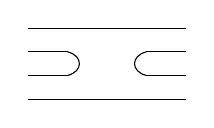
\begin{tikzpicture}
					\draw (0, 0) -- (2, 0);
					\draw (0, 0.3) -- (0.5, 0.3);
					\draw (0, 0.6) -- (0.5, 0.6);
					\draw (0.5, 0.3) .. controls (0.7, 0.35) and (0.7, 0.55) .. (0.5, 0.6);
					\draw (1.5, 0.3) -- (2, 0.3);
					\draw (1.5, 0.6) -- (2, 0.6);
					\draw (1.5, 0.3) .. controls (1.3, 0.35) and (1.3, 0.55) .. (1.5, 0.6);
					\draw (0, 0.9) -- (2, 0.9);
				\end{tikzpicture}
				\caption{Generator $U_2$ in TL$_4(\delta)$.}
				\label{fig:generator_temperley_lieb}
			\end{subfigure}
        	\end{figure}
        }

\subsection{Graded vector spaces}\label{section:graded_spaces}

	Similar to definition \ref{group:graded_ring} we can define the following:
	\newdef{Graded vector space}{\index{degree}\index{graded!vector space}
		Let $V_n$ be a vector space for all $n\in\mathbb{N}$. The vector space
		\begin{gather}
			\label{linalgebra:graded_vector_space}
			V = \bigoplus_{n\in\mathbb{N}} V_n
		\end{gather}
		is called a graded vector space. In fact one can replace $\mathbb{N}$ by any countable (finite or infinite) index set. For most operations however one requires the index set to be closed under addition operations. The index $n$ is often called the \textbf{degree} of the subspace $V_n$ in $V$.
	}
	
	\newdef{Graded algebra}{\index{graded!algebra}
		Let $V$ be a graded vector space with the additional structure of an algebra given by the multiplication $\star$. Then $V$ is a graded algebra if $\star$ maps $V^k\times V^l$ to $V^{k+l}$.
	}
	
	\newdef{Super vector space}{\index{super!vector space}
		A super vector space is defined as a $\mathbb{Z}_2$-graded vector space.
	}
	
	\begin{example}[Superalgebra]\index{super!algebra}\label{linalgebra:superalgebra}
		A $\mathbb{Z}_2$-graded algebra, i.e. there exists a decomposition
		\begin{gather}
			A = A_0\oplus A_1
		\end{gather}
		such that for all $i, j \mod 2$:
		\begin{gather}
			A_i\star A_j \subseteq A_{i+j}
		\end{gather}
	\end{example}
	
	\newdef{dg-algebra}{\index{dg-algebra}\label{linalgebra:dg_algebra}
		A differential graded algebra (often denoted by dg-algebra) is a graded algebra equipped with a differential of degree 1.
	}
	
	\newdef{Parity functor}{\index{parity}
		Consider the category $\mathbf{sVect}$ of super vector spaces. We can define the parity functor $\func{\Pi}{sVect}{sVect}$ as the functor which interchanges even and odd subspaces:
		\begin{align}
			(\Pi V)_0 &= V_1\\
			&\\
			(\Pi V)_1 &= V_0
		\end{align}
	}
	\newdef{Symmetric tensors}{
		Using the parity functor one can write the exterior algebra $\Lambda^\bullet(V)$ as the symmetric algebra $\text{Sym}^\bullet(\Pi V)$. In a similar way one can write the symmetric algebra on a super vector space $V=V_0\oplus V_1$ as $\text{Sym}^n(V)=\bigoplus_{p+q=n}\text{Sym}^p(V_0)\otimes\Lambda^q(V_1)$.
	}
        
\section[Linear maps]{Linear maps\footnote{Other names are \textbf{linear mapping} and \textbf{linear transformation}.}}

	\newdef{Injective}{\label{linalgebra:injective}
		A map $f:A\rightarrow B$ is called injective if the following condition is satisfied:
	    	\begin{gather}
		        \forall a, a'\in A:f(a)=f(a')\implies a=a'
		\end{gather}
	}
	\newnot{Injective map}{\[f:A\hookrightarrow B\]}
	\newdef{Surjective}{\label{linalgebra:surjective}
		A map $f:A\rightarrow B$ is called surjective if the following condition is satisfied:
	    	\begin{gather}
		        \forall b\in B, \exists a\in A:f(a) = b
		\end{gather}
	}
	\newnot{Surjective map}{\[f:A\twoheadrightarrow B\]}
	\newnot{Bijective map}{\[f:A\xrightarrow{\sim} B\qquad\text{or}\qquad f:A\cong B\]}
	\newnot{Isomorphic}{If two $K$-vector spaces $V, W$ are isomorphic we denote this by\[V\cong W\]}
	
	\begin{property}
		Let $V$ be finite-dimensional $K$-vector space. Let $f:V\rightarrow V$ be a linear map. The following statements are equivalent:
        	\begin{itemize}
            		\item $f$ is injective
			\item $f$ is surjective
                	\item $f$ is bijective
		\end{itemize}
	\end{property}

	\newdef{Automorphism}{\index{automorphism}\label{linalgebra:automorphism}
		\nomenclature[S_Aut]{$\text{Aut}(V)$}{Set of automorphisms (invertible endomorphisms) on a set $V$.}
	    	An isomorphism from $V$ to $V$ is called an automorphism\footnote{In some case also called a \textbf{linear operator}, but this terminology is also often used for a general linear map in \textit{operator theory}.}. The set of all automorphisms  on $V$, which is in fact a group, is denoted by $\text{Aut}(V)$.
	}
    
	\newdef{General linear group\footnotemark}{\index{general linear group}
		\nomenclature[S_GL]{GL$(V)$}{General linear group: group of all automorphisms on a vector space $V$.}
		\footnotetext{This group is isomorphic to the general linear group of invertible matrices, hence the similar name and notation. (See definition \ref{linalgebra:GL_matrices})}
	    	The set of all automorphisms $f:V\rightarrow V$ is called the general linear group and denoted by GL$_K(V)$ or GL$(V)$ when the base field is obvious.
	}

	\newdef{Rank}{\index{rank}\label{linalgebra:image_rank}
		The dimension of the image of a linear map is called the rank.
	}
	\newdef{Kernel}{\index{kernel}
	        The kernel of a linear map $f: V \rightarrow W$ is the following subset of $V$:
        	\begin{gather}
        		\text{ker}(f) = \{v\in V\ |\ f(v) = 0\}
	        \end{gather}
	}
	\newdef{Nullity}{\index{nullity}
		The dimension of the kernel is called the nullity.
	}
    
	\begin{theorem}
	    	A linear map $f:V\rightarrow W$ is injective if and only if $\text{ker}(f) = \{0\}$.
	\end{theorem}
	\begin{property}
	        Let $f:V\rightarrow W$ be a linear map. Let $U\leq V$. We have the following two properties of the restriction $f|_U$ of $f$ to $U$:
        	\begin{itemize}
			\item $\text{ker}\left(f|_U\right) = \text{ker}(f)\cap U$
        		\item $\text{im}\left(f|_U\right) \leq \text{im}(f)$
		\end{itemize}
	\end{property}
    
\subsection{Dimension}

        \begin{theorem}[Dimension theorem\footnotemark]\index{rank-nullity theorem}
		\footnotetext{Also called the \textbf{rank-nullity theorem}.}
		Let $f: V \rightarrow W$ be a linear map.
	        \begin{gather}
	                \label{linalgebra:dimension_theorem}
	                \dim(\text{\upshape im}(f)) + \dim(\text{\upshape ker}(f)) = \dim(\text{\upshape V})
	        \end{gather}
        \end{theorem}

        \begin{property}
		Two $K$-vector spaces are isomorphic if and only if they have the same dimension.
	\end{property}

\section{Inner product}\label{linalgebra:innerproduct}
	In the following section all vector spaces $V$ will be $\mathbb{R}$- or $\mathbb{C}$-vector spaces.
    
	\newnot{Inner product}{\index{inner!product}
		Let $v, w$ be two vectors in $V$. The map $\langle \cdot|\cdot \rangle:V\times V\rightarrow K$ is called an inner product on $V$ if it satisfies the following 3 properties:
		\begin{enumerate}
			\item \textbf{Conjugate symmetry:} $\langle v|w\rangle = \langle w|v\rangle^*$
			\item \textbf{Linearity in the first argument:} $\langle \lambda u + v|w\rangle = \lambda\langle u|w\rangle + \langle v|w\rangle$
			\item \textbf{Non-degeneracy: } $\langle v|v\rangle = 0 \iff v = 0$
			\item \textbf{Positive-definiteness} $\langle v|v\rangle \geq 0$
		\end{enumerate}
	}
	\remark{\index{Hermitian!form}
		\label{linalgebra:NDH_form}
    		Inner products are special cases of \textbf{non-degenerate Hermitian forms} which do not possses the positive-definiteness property.
	}

	\begin{result}
    		The first two properties have the result of conjugate linearity in the second argument:
    		\begin{equation}
			\langle f|\lambda g + \mu h\rangle = \overline{\lambda}\langle f|g \rangle + \overline{\mu}\langle f|h \rangle
		\end{equation}
	\end{result}
    
\subsection{Inner product space}
	
	\newdef{Inner product space\footnotemark}{
		\footnotetext{Sometimes called a \textbf{prehilbert space}.}
		A vector space equipped with an inner product $\langle\cdot|\cdot\rangle$ is called an inner product space.
	}

        \newdef{Metric dual\footnotemark}{\footnotetext{See also definition \ref{manifolds:flat_map}.}
        	Using the inner product (or any other non-degenerate Hermitian form) one can define the metric dual of a vector $v$ by the following map:
            \begin{equation}
            	\label{linalgebra:metric_dual}
            	L:V\rightarrow V^*:v\mapsto \langle v|\cdot \rangle
            \end{equation}
        }
        \newdef{Adjoint operator}{\index{Hermitian!adjoint}\index{self-adjoint}\label{linalgebra:adjoint_operator}
		Let $A$ be a linear operator on $V$. Let $v, w$ be two vectors in $V$. The \textit{Hermitian} adjoint of $A$ is defined as the linear operator $A^\dag$ that satisfies:
		\begin{equation}
			\langle A^\dag v, w\rangle = \langle v, Aw\rangle
		\end{equation}
		Alternatively one can define the adjoint using the metric dual $L(\cdot)$ as follows:
		\begin{equation}
			\boxed{A^\dag = L^{-1} \circ A^T \circ L}
		\end{equation}
		If $A = A^\dag$ then A is said to be \textbf{Hermitian} or \textbf{self-adjoint}.
	}
	
    \begin{result}
    	The Hermitian adjoint of a complex matrix $A\in\mathbb{C}^{m\times n}$ is given by:
        \begin{equation}
			A^\dag = \overline{A}^T
		\end{equation}
        where $\overline{A}$ denotes the complex conjugate of $A$ and $A^T$ the transpose of $A$.
    \end{result}
    
	The definition of an adjoint operator \ref{linalgebra:adjoint_operator} can be generalized to the case where $A^\dag$ is not unique (for example when $A$ is not globally defined) in the following way:
	\newdef{Conjugate operators}{
		Two operators $B$ and $C$ are said to be conjugate if:
		\begin{equation}
			\langle Bx, y\rangle = \langle x, Cy\rangle
		\end{equation}
	}
    
    \begin{example}\index{Lie!algebra}\index{isometry}
    	The Lie algebra associated with the group of isometries $\text{Isom}(V)$ of a non-degenerate Hermitian form satisfies following condition:
        \begin{equation}
        	\label{linalgebra:lie_isometry}
        	\langle Xv, w \rangle = -\langle v, Xw \rangle
        \end{equation}
        for all Lie algebra elements $X$. It follows that the Lie algebra consists of all anti-hermitian operators.
    \end{example}
    
\subsection{Orthogonality}\label{linalgebra:section:orthogonality}
	
	\newdef{Orthogonal}{
		Let $v, w \in V$. The vectors $v$ and $w$ are said to be orthogonal, denoted by $v\perp w$,  if they obey the following relation:
		\begin{equation}
			\label{linalgebra:orthogonal}
			\langle v|w \rangle = 0
		\end{equation}
		An orthogonal \textbf{system} is a set of vectors, none of them the null vector, that are mutually orthogonal.
	}
	\begin{property}
		Orthogonal systems are linearly independent.
	\end{property}
	
	\newdef{Orthonormal}{
		A set of vectors $\{v_n\}$ is said to be orthonormal if it is orthogonal and if all the elements $v_n$ obey the following relation:
		\begin{equation}
			\label{linalgebra:orthonormal}
			\langle v|v \rangle = 1
		\end{equation}
	}
        \newdef{Orthogonal complement\footnotemark}{\label{linalgebra:orthogonal_complement}Let $W$ be a subspace of $V$. The following subspace is called the orthogonal complement of $W$:
        	\begin{equation}
                W^\perp = \{v\in V\ |\ \forall w\in W:\langle v|w\rangle = 0\}
			\end{equation}
        }
        \footnotetext{$W^\perp$ is pronunciated as 'W-perp'.}
        
        	\begin{property}
		The inner-product is invariant under transformations between orthonormal bases.
	\end{property}
        
        \begin{property}
        	\label{linalgebra:W_W_perp_intersection}
			\begin{equation}
				W \cap W^\perp = \{0\}
			\end{equation}
		\end{property}
        \begin{property}
			Let $V$ be a finite-dimensional K-vector space. The orthogonal complement $W^\perp$ is a complementary subspace\footnotemark\ to W, i.e. $W\leq V$: $W\oplus W^\perp=V$.
		\end{property}
        \footnotetext{hence the name}
        \begin{result}
        	\label{linalgebra:perp_of_perp}
			Let $W\leq V$ where $V$ is a finite-dimensional K-vector space. We have the following relation:
            \begin{equation}
	            (W^\perp)^\perp = W
			\end{equation}
		\end{result}
    
    	\newdef{Orthogonal projection}{\index{projection}\label{linalgebra:orthogonal_projection}
    	Let $V$ be a finite-dimensional K-vector space. Let $W\leq V$. Let $w\in W$ and let $\{w_1, ..., w_k\}$ be an orthonormal basis of $W$. We define the projection of $v\in V$ on $W$ and $w\in W$ as follows:
        	\begin{equation}
				\text{proj}_W(v) = \sum_{i=1}^k\langle v|w_i \rangle w_i
			\end{equation}
            \begin{equation}
				\text{proj}_w(v) = \stylefrac{\langle v|w \rangle}{\langle w|w \rangle}w
			\end{equation}
        }
        \begin{property}\ 
			\begin{enumerate}
				\item $\forall w\in W:\text{proj}_W(w) = w$
                \item $\forall u\in W^\perp:\text{proj}_W(u) = 0$
			\end{enumerate}
		\end{property}
        
	\newmethod{Gram-Schmidt orthonormalisation}{
		Let $\{u_n\}$ be a set of linearly independent vectors. We can construct an orthonormal set $\{e_n\}$ out of $\{u_n\}$ in the following way:
		\begin{equation}
			\label{linalgebra:inner_product:gramm_schmidt}
			\begin{aligned}
				&w_1 = u_1&\\
				&w_2 = u_2 - \stylefrac{\langle u_2|w_1\rangle}{||u_2||^2}w_1&\\
				&\vdots&\\
				&w_n = u_n - \sum_{k = 1}^{n-1}\stylefrac{\langle u_n|w_k\rangle}{||u_n||^2}w_k&
			\end{aligned}\qquad
			\begin{aligned}
				&e_1 = \stylefrac{w_1}{||w_1||}&\\
				&e_2 = \stylefrac{w_2}{||w_2||}&\\
				&\vdots&\\
				&e_n = \stylefrac{w_n}{||w_n||}&
			\end{aligned}
		\end{equation}
	}
	
	\newdef{Householder transformation}{\index{Householder transformation}\label{linalgebra:householder_transformation}
		Let $v$ be an element of an inner product space $V$. The Householder transformation generated by $v$ is given by the linear map
		\begin{equation}
			\sigma_v:w\mapsto w - 2\frac{\langle w|v \rangle}{\langle v|v \rangle}v
		\end{equation}
		This transformation amounts to a reflection in the hyperplane orthogonal to $v$.
	}
        
\subsection{Angle}
	
	\newdef{Angle}{\index{angle}
		Let $v,w$ be elements of an inner product space $V$. The angle $\theta$ between $v$ and $w$ is defined as:
		\begin{equation}
			\label{linalgebra:angle}
			\boxed{\cos\theta = \stylefrac{\langle v|w \rangle}{||v||||w||}}
		\end{equation}
	}

\section{Matrices}
	
	\begin{notation}\label{linalgebra:matrix_set}
	        The set of all $m\times n$-matrices defined over the field K is denoted by $M_{m,n}(K)$. If $m=n$, the set is denoted by $M_n(K)$.
	\end{notation}
	
	\begin{property}[Dimension]\index{dimension}\label{linalgebra:dimension_of_matrix_space}
		The dimension of $M_{m,n}(K)$ is $mn$.
	\end{property}
    
	\newdef{Trace}{\index{trace}\label{linalgebra:trace}
	        Let $A = (a_{ij})\in M_n(K)$. We define the trace of $A$ as follows:
    		\begin{equation}
			\boxed{\operatorname{tr}(A) = \sum_{i=1}^na_{ii}}
		\end{equation}
	}
	\begin{property}\label{linalgebra:trace_commutative}
		Let $A, B\in M_n(K)$. We have the following properties of the trace:
	        \begin{enumerate}
        		\item $\text{tr}:M_n(K)\rightarrow K$ is a linear map
			\item $\text{tr}(AB) = \text{tr}(BA)$
			\item $\text{tr}(AB) \neq \text{tr}(A)\text{tr}(B)$
        		\item $\text{tr}(A^T) = \text{tr}(A)$
		\end{enumerate}
	\end{property}
    
	\newformula{Hilbert-Schmidt norm\footnotemark}{\index{Frobenius!norm}\index{Hilbert-Schmidt norm}
    		\footnotetext{Also called the \textbf{Frobenius norm}.}
    		The Hilbert-Schmidt matrix norm is given by following formula:
	        \begin{equation}
        		\label{linalgebra:hilbert_schmidt_norm}
        		||A||^2_{HS} = \sum_{i, j}|A_{ij}|^2 = \text{tr}(A^\dag A)
	        \end{equation}
        	If one identifies $M_{n}(\mathbb{C})$ with $\mathbb{C}^{2n}$ then this norm equals the standard Hermitian norm.
	}

	\newformula{Hadamard product}{\index{Hadamard!product}
    		The Hadamard product of two matrices $A, B\in M_{m\times n}(K)$ is defined as the entry-wise product:
        	\begin{equation}
        		(A\circ B)_{ij} = A_{ij}B_{ij}
        	\end{equation}
	}
    
	\newdef{General linear group}{\index{general linear group}\label{linalgebra:GL_matrices}
		\nomenclature[S_GLn]{GL$_n(K)$}{General linear group: group of all invertible $n$-dimensional matrices over the field $K$.}
	        The set of invertible matrices is called the general linear group and is denoted by GL$_n(K)$.
	}
	\begin{property}
		For all $A\in\text{GL}_n(K)$ we have:
	        \begin{itemize}
			\item $A^T\in\text{GL}_n(K)$
		        \item $\left(A^T\right)^{-1}=\left(A^{-1}\right)^T$
		\end{itemize}
	\end{property}
    
	\begin{property}\label{linalgebra:dim_columns_rows}
		Let $A\in M_{m,n}(K)$. Denote the set of columns as $\{A_1, A_2, ..., A_n\}$ and the set of rows as $\{R_1, R_2, ..., R_m\}$. The set of columns is a subset of $K^m$ and the set of rows is a subset of $K^n$. Furthermore we have:
		\[
			\dim(\text{span}(A_1, ..., A_n)) = \dim(\text{span}(R_1, ..., R_m))
		\]
	\end{property}
	
	\newdef{Rank of a matrix}{\index{rank}
		We can define the rank of matrix $A\in M_{m,n}(K)$ as follows:
		\begin{equation}
			\label{linalgebra:matrix_rank}
        			\text{rk}(A) := \dim(\text{span}(A_1, ..., A_n)) \overset{\ref{linalgebra:dim_columns_rows}}{=} \dim(\text{span}(R_1, ..., R_m))
		\end{equation}
	}
    
	\begin{property}\label{linalgebra:rank_properties}
	        The rank of a matrix has the folowing properties:
        	\begin{enumerate}
			\item Let $A\in M_{m,n}(K)$ and $B\in M_{n,r}(K)$. We have $\text{rk}(AB)\leq\text{rk}(A)$ and $\text{rk}(AB)\leq\text{rk}(A)$.
        		\item Let $A\in\text{GL}_n(K)$ and $B\in M_{n,r}(K)$. We have $\text{rk}(AB)=\text{rk}(B)$.
		        \item Let $A\in\text{GL}_n(K)$ and $B\in M_{r,n}(K)$. We have $\text{rk}(BA)=\text{rk}(B)$.
		\end{enumerate}
	\end{property}
	\begin{property}\label{linalgebra:dim_matrix_left_multiplication}
	        Let $A\in M_{m,n}(K)$. First define the following linear map:
        	\begin{equation}
			\label{linalgebra:matrix_left_multiplication}
        		\boxed{L_A:K^n\rightarrow K^m:v\mapsto Av}
		\end{equation}
	        This map has the following properties:
        	\begin{enumerate}
        		\item $\text{im}(L_A) = \text{span}(A_1, ..., A_n)$
			\item $\dim(\text{im}(L_A))=\text{rk}(A)$
		\end{enumerate}
	\end{property}
	\sremark{The second property is a direct consequence of the first one and definition \ref{linalgebra:matrix_rank}.}
    
\subsection{System of equations}

	\begin{theorem}\label{linalgebra:matrix_and_equations}
	        Let $AX=w$ with $A\in M_{m,n}(K)$, $w\in K^m$ and $X\in K^n$ be a system of $m$ equations in $n$ variables. Let $L_A$ be the linear map as defined in equation \ref{linalgebra:matrix_left_multiplication}. We then have the following properties:
        	\begin{enumerate}
			\item The system is false if and only if $w\not\in\text{im}(L_A)$.
        		\item If the system is not false, the solution set is an affine space. If $v_0\in K^n$ is a solution, then the solution set is given by: $L_A^{-1}(w)=v_0+\text{ker}(L_A)$.
		        \item If the system is homogeneous ($AX=0$), then the solution set is equal to $\text{ker}(L_A)$.
		\end{enumerate}
	\end{theorem}
	\begin{theorem}[Uniqueness]\label{linalgebra:rank_unique_solution}
	        Let $AX=w$ with $A\in M_n(K)$ be a system of $n$ equations in $n$ variables. If $\text{rk}(A)=n$, then the system has a unique solution.
	\end{theorem}
    
\subsection{Coordinates and matrix representations}

        \newdef{Coordinate vector}{\label{linalgebra:coordinate_vector}
        	Let $\mathcal{B} = \{b_1, ..., b_n\}$ be a basis of $V$. Let $v\in V$ such that $v=\sum_{i=1}^n\lambda_ib_i$. We define the coordinate vector of $v$ with respect to $\mathcal{B}$ as $(\lambda_1, ..., \lambda_n)^T$. The $\lambda_i$'s are called the \textbf{coordinates} of $v$ with respect to $\mathcal{B}$.
        }
        \newdef{Coordinate isomorphism}{\label{linalgebra:coordinate_isomorphism}
        	With the previous definition in mind we can define the coordinate isomorphism of $v$ with respect to $\mathcal{B}$ as follows:
        	\begin{equation}
			\boxed{\beta:V\rightarrow K^n:\sum_{i=1}^n\lambda_ib_i\mapsto(\lambda_1, ..., \lambda_n)^T}
		\end{equation}
        }
        
        \newdef{Matrix representation}{\label{linalgebra:matrix_representation}
        	Let $V$ be an $n$-dimensional K-vector space and $W$ an $m$-dimensional K-vector space. Let $f:V\rightarrow W$ be a linear map. Let $\mathcal{B}=\{b_1, ..., b_n\}, \mathcal{C} = \{c_1, ..., c_m\}$ be a basis for $V$, respectively $W$. The matrix representation of $f$ with respect to $\mathcal{B}$ and $\mathcal{C}$ can be derived as follows: For every $j\in\{1, ..., n\}$ we can write $f(b_j) = \sum_{i=1}^ma_{ij}c_i$, so with this in mind we can define the matrix $(a_{ij})\in M_{m,n}(K)$ as the matrix represenation of $f$.
        }
        \newnot{Matrix representation of a linear map}{
        	The matrix representation of $f$ with respect to $\mathcal{B}$ and $\mathcal{C}$ is denoted by $A_{f, \mathcal{B}, \mathcal{C}}$.
        }
        
        \newmethod{Construction of a matrix representation}{\label{linalgebra:method:matrix_representation}
        	From definition \ref{linalgebra:matrix_representation} we can see that $j$-th column of $A_{f, \mathcal{B}, \mathcal{C}}$ coincides with the coordinate vector of $f(b_j)$ with respect to $\mathcal{C}$. We use this relation to construct $A_{f, \mathcal{B}, \mathcal{C}}$ by writing for every $j\in\{1, ..., n\}$ the coordinate vector of $f(b_j)$ in the $j$-th column.
        }
        
        \begin{theorem}\label{linalgebra:theorem:matrix_representation}
		Let $(\lambda_1, ..., \lambda_n)^T$ be the coordinate vector of $v\in V$ with respect to $\mathcal{B}$. Let $(\mu_1, ..., \mu_m)^T$ be the coordinate vector of $f(v)$ with respect to $\mathcal{C}$. Then the following relation holds:
            	\begin{equation}
			\left(
			\begin{array}{c}
				\mu_1\\
				\vdots\\
				\mu_m
			\end{array}\right)
	                = A_{f, \mathcal{B}, \mathcal{C}}
        	        \left(\begin{array}{c}
				\lambda_1\\
				\vdots\\
				\lambda_n
			\end{array}\right)
		\end{equation}
	\end{theorem}
        
        \begin{theorem}\label{linalgebra:theorem:map_matrix_link}
		For every matrix $A\in M_{m,n}(K)$ there exists a linear map $f:V\rightarrow W$ such that $A_{f, \mathcal{B}, \mathcal{C}} = A$.
	\end{theorem}
        On the other hand we also have the following theorem:
        \begin{theorem}
		Let $f:K^n\rightarrow K^m$ be a linear map. There exists a matrix $A\in M_{m,n}(K)$ such that $f=L_A$.
	\end{theorem}
        \begin{theorem}
		Let $\beta$ and $\gamma$ be the coordinate isomorphisms with respect to respectively $\mathcal{B}$ and $\mathcal{C}$. From theorem \ref{linalgebra:theorem:matrix_representation} it follows that:
        	\begin{equation}
			\gamma(f(v)) = A_f\cdot\beta(v)
		\end{equation}
        	or alternatively
        	\begin{equation}
			\gamma\circ f = L_{A_f}\circ\beta
		\end{equation}
	\end{theorem}
        
        \begin{theorem}\label{linalgebra:theorem:matrix_composition_hom}
	        The map $\text{Hom}_K(V,W)\rightarrow M_{m,n}(K):f\mapsto A_f$ is an isomorphism and for every $f\in\text{Hom}_K(V,W)$ and $g\in \text{Hom}_K(W,U)$ we have:
		\begin{equation}
			A_{g\circ f} = A_gA_f
		\end{equation}
	\end{theorem}
	
	\begin{theorem}\label{linalgebra:theorem:matrix_composition_end}
	        The map $\text{End}_K(V)\rightarrow M_n(K):f\mapsto A_{f, \mathcal{B}, \mathcal{B}}$ is an isomorphism and for every $f,g\in\text{End}_K(V)$ we have:
        	\begin{equation}
			A_{g\circ f} = A_gA_f
		\end{equation}
	\end{theorem}
	
        \begin{theorem}\label{linalgebra:matrix_invertable_map}
	        Let $f\in\text{End}_K(V)$. Let $A_f$ be the corresponding matrix representation. The linear map $f$ is invertible if and only if $A_f$ is invertible. Furthermore, if $A_f$ is invertible, we have that \[\left(A_f\right)^{-1} = A_{f^{-1}}\] In other words, the following map is an isomorphism\footnotemark:
	        \begin{equation}
	        	\text{GL}_K(V)\rightarrow\text{GL}_n(K):f\mapsto A_f
	        \end{equation}
	        \footnotetext{Follows from theorem \ref{linalgebra:theorem:matrix_composition_end}.}
	\end{theorem}
        \remark{The sets GL$_K(V)$ and GL$_N(K)$ are groups. So the previous theorem states that the map $f\mapsto A_f$ is a group isomorphism.}
        
        \begin{theorem}
		Let $V = K^n$. Let $f\in V^*$. From construction \ref{linalgebra:method:matrix_representation} it follows that $A_f = (f(e_1), ..., f(e_n))\in M_{1,n}(K)$ with respect to the standard basis of $V$. This combined with theorem \ref{linalgebra:theorem:matrix_representation} gives:
	        \begin{equation}
			f(\lambda_1, ..., \lambda_n)^T = (f(e_1), ..., f(e_n))(\lambda_1, ..., \lambda_n)^T = \sum_{i=1}^nf(e_i)\lambda_i
		\end{equation}
        	or alternatively with $\{\varepsilon_1, ..., \varepsilon_n\}$ the dual basis to the standard basis of $V$:
	        \begin{equation}
        	    	\label{linalgebra:map_in_function_of_dual_basis}
			\boxed{f = \sum_{i=1}^nf(e_i)\varepsilon_i}
		\end{equation}
	\end{theorem}
        
        \begin{theorem}
		Let $f:V\rightarrow W$ be a linear map. Let $f^*:W^*\rightarrow V^*$ be the corresponding dual map. If $A_f$ is the matrix representation of $f$ with respect to $\mathcal{B}$ and $\mathcal{C}$, then the transpose $A_f^T$ is the matrix representation of $f^*$ with respect to the dual basis of $\mathcal{C}$ and the dual basis of $\mathcal{B}$.
	\end{theorem}
        
\subsection{Coordinate transforms}
        
        \newdef{Transition matrix}{\label{linalgebra:transition_matrix}
        	Let $\mathcal{B} = \{b_1, ..., b_n\}$ and $\mathcal{B}' = \{b_1', ..., b_n'\}$ be two bases of $V$. Every element of $\mathcal{B}'$ can be written as a linear combination of elements in $\mathcal{B}$:
        	\begin{equation}
        		b_j' = q_{1j}b_1 + ... + q_{nj}b_n
        	\end{equation}
	        The matrix $Q = (q_{ij})\in M_n(K)$ is called the transition matrix from the 'old' basis $\mathcal{B}$ to the 'new' basis $\mathcal{B}'$.}
        
        \begin{theorem}\label{linalgebra:theorem:transition_matrix}
		Let $\mathcal{B}, \mathcal{B}'$ be two basis of $V$. Let $Q$ be the transition matrix from $\mathcal{B}$ to $\mathcal{B}'$. We find the following statements:
	        \begin{enumerate}
			\item Let $\mathcal{C}$ be an arbitrary basis of $V$ with $\gamma$ the corresponding coordinate isomorphism. Define the following matrices:
        	        	\[
        	        		B=(\gamma(b_1), ..., \gamma(b_n))\quad\text{and}\quad B'=(\gamma(b_1'), ..., \gamma(b_n'))
        	        	\]
		                Then $BQ = B'$.
			\item $Q\in\text{GL}_n(K)$ and $Q^{-1}$ is the transition matrix from $\mathcal{B}'$ to $\mathcal{B}$.
                	\item Let $v\in V$ with $(\lambda_1, ..., \lambda_n)^T$ the coordinate vector with respect to $\mathcal{B}$ and $(\lambda_1', ..., \lambda_n')^T$ the coordinate vector with respect to $\mathcal{B}'$. Then:
                	\[
		                Q\left(
				\begin{array}{c}
					\lambda_1'\\
                			\vdots\\
			        	\lambda_n'
				\end{array}
                        	\right)
                        	=
		                \left(
                		\begin{array}{c}
					\lambda_1\\
                			\vdots\\
			        	\lambda_n
				\end{array}
                        	\right)
				\quad\text{and}\quad
                        	\left(
                        	\begin{array}{c}
					\lambda_1'\\
                        		\vdots\\
			        	\lambda_n'
				\end{array}
		                \right)
                	        =
                	        Q^{-1}\left(
                	        \begin{array}{c}
					\lambda_1\\
                		        \vdots\\
			                \lambda_n
				\end{array}
                        	\right)
			\]
		\end{enumerate}
	\end{theorem}
        
	\begin{theorem}\label{linalgebra:theorem:transition_matrix_representation}
        	Let $V,W$ be two finite-dimensional K-vector spaces. Let $\mathcal{B}, \mathcal{B}'$ be two bases of $V$ and $\mathcal{C}, \mathcal{C}'$ two bases of $W$. Let $Q, P$ be the transition matrices from $\mathcal{B}$ to $\mathcal{B}'$ and from $\mathcal{C}$ to $\mathcal{C}'$ respectively. Let $A=A_{f, \mathcal{B}, \mathcal{C}}$ and $A' = A_{f, \mathcal{B}', \mathcal{C}'}$. Then:
	        \begin{equation}
        	    	A' = P^{-1}AQ
        	\end{equation}
	\end{theorem}
        \begin{result}
		Let $f\in \text{End}_K(V)$ and let $Q$ be the transition matrix. From theorem \ref{linalgebra:theorem:transition_matrix_representation} it follows that:
            	\begin{equation}
	            	A'=Q^{-1}AQ
        	\end{equation}
	\end{result}

        \newdef{Matrix conjugation}{\index{conjugacy class}\index{matrix!conjugation}\label{linalgebra:conjugacy_class}
        	Let $A\in M_n(K)$. The set
        	\begin{equation}
	            	\{Q^{-1}AQ\ |\ Q\in\text{GL}_n(K)\}
        	\end{equation}
	        is called the conjugacy class\footnotemark\ of $A$. Another name for conjugation is \textbf{similarity transformation}.
        	\footnotetext{This is the general definition of conjugacy classes for groups. Furthermore, these classes induce a partitioning of the group.}
	}
        \begin{remark}
        	If $A$ is a matrix representation of a linear operator $f$, then the conjugacy class of $A$ consists out of every possible matrix representation of $f$.
        \end{remark}
        
        \begin{property}\index{trace}
        	From property \ref{linalgebra:trace_commutative} it follows that the trace of a matrix is invariant under similarity transformations:
        	\begin{equation}
            		\label{linalgebra:trace_invariance}
            		\boxed{\text{tr}(Q^{-1}AQ) = \text{tr}(A)}
	        \end{equation}
        \end{property}
        
        \newdef{Matrix congruence}{\index{matrix!congruence}\label{linalgebra:matrix_congruence}
        	Let $A, B\in M_n(K)$. If there exists a matrix $P$ such that
	        \begin{equation}
        	    	A = P^TBP
        	\end{equation}
	        then the matrices are said to be congruent.
        }
        \begin{property}
        	Every matrix congruent to a symmetric matrix is also symmetric.
        \end{property}
        
        \begin{theorem}\label{linalgebra:theorem:orthogonal_transition_matrix}
        	Let $(V, \langle .|. \rangle)$ be an inner-product space defined over $\mathbb{R}$ (or $\mathbb{C}$). Let $\mathcal{B}, \mathcal{B}'$ be two orthonormal bases of $V$ and let $Q$ be the transition matrix. Then $Q$ is orthogonal:
        	\begin{equation}
	        	Q^TQ = \mathbbm{1}_n
	        \end{equation}
	\end{theorem}

\subsection{Determinant}

    	\newdef{Minor}{
        	The $(i, j)$-th minor of $A$ is defined as:\[\det(A_{ij})\] where $A_{ij}\in M_{n-1}(K)$ is the matrix obtained by removing the $i$-th row and the $j$-th column from $A$.
	}
        \newdef{Cofactor}{
        	The cofactor $\alpha_{ij}$ of the matrix element $a_{ij}$ is equal to:\[(-1)^{i+j}\det(A_{ij})\]where $\det(A_{ij})$ is the minor as previously defined.
	}
        \newdef{Adjugate matrix}{\label{linalgebra:adjugate_matrix}
	        The adjugate matrix of $A\in M_n(K)$ is defined as follows:
	       	\begin{equation}
	            	\text{adj}(A) := \left(
	                \begin{array}{cccc}
				\alpha_{11}&\alpha_{21}&\dotsm&\alpha_{n1}\\
		                \alpha_{12}&\alpha_{22}&\dotsm&\alpha_{n2}\\
		                \vdots&\vdots&\vdots&\vdots\\
		                \alpha_{1n}&\alpha_{2n}&\dotsm&\alpha_{nn}\\
			\end{array}
        	        \right)
		\end{equation}
        	or shorter: $\text{adj}(A) = (\alpha_{ij})^T$.
        }
        \begin{remark*}
		It is important to notice that we have to transpose the matrix after the elements have been replaced by their cofactor.
	\end{remark*}
        
        \begin{property}\label{linalgebra:determinant_properties}
	        Let $A,B\in M_n(K)$. Denote the columns of $A$ as $A_1, \dotso, A_n$. We have the following properties of the determinant:
	        \begin{enumerate}
			\item $\det(A^T) = \det(A)$
	                \item $\det(AB) = \det(BA) = \det(A)\det(B)$
	                \item $\det(A_1, \dotso, A_i+\lambda A_i', \dotso, A_n) = \det(A_1, \dotso, A_i, \dotso, A_n) + \lambda\det(A_1, \dotso,A_i', \dotso, A_n)$ for all $A_i,A_i'\in M_{n,1}(K)$.
	                \item If two columns of $A$ are equal then $\det(A) = 0$.
	                \item $\det(A_{\sigma(1)},\dotso,A_{\sigma(n)}) = \text{sgn}(\sigma)\det(A_1,\dotso,A_n)$
	                \item The determinant can be evaluated as follows:
	                	\begin{equation}
					\det(A) = \sum_{i=1}^n(-1)^{i+k}a_{ik}\det(A_{ik})
				\end{equation}
		\end{enumerate}
		\end{property}
        
	\begin{theorem}\label{linalgebra:theorem:rank_det_equivalence}
        	Let $A\in M_n(K)$, the following statements are equivalent:
        	\begin{enumerate}
			\item $\det(A) \neq 0$
        	        \item $\text{rk}(A) = n$
        	        \item $A\in\text{GL}_n(K)$
		\end{enumerate}
	\end{theorem}
        \begin{theorem}\label{linalgebra:theorem:adjugate_matrix}
            For all $A\in M_n(K)$ we find $A\text{adj}(A) = \text{adj}(A)A = \det(A)I_n$.
	\end{theorem}
        \begin{formula}\label{linalgebra:theorem:determinant_inverse}
	        For all $A\in\text{GL}_n(K)$ we find:
		\begin{equation}
            		A^{-1} = \det(A)^{-1}\ \text{adj}(A)
            	\end{equation}
	\end{formula}
        
        An alternative definition of a $k\times k$-minor is: 
        \begin{definition}
		Let $A\in M_{m,n}(K)$ and $k\leq\min(m, n)$. A $k\times k$-minor of $A$ is the determinant of a $k\times k$-partial matrix obtained by removing $m-k$ rows and $n-k$ columns from $A$.
	\end{definition}
        \begin{theorem}
		Let $A\in M_{m,n}(K)$ and $k\leq\min(m, n)$. We find that $\text{rk}(A)\geq k$ if and only if $A$ contains a non-zero $k\times k$-minor.
	\end{theorem}
        
        \begin{theorem}
		Let $f\in\textup{End}_K(V)$. The determinant of the matrix representation of $f$ is invariant under basis transformations.
	\end{theorem}
	
        \newdef{Determinant of a linear operator}{\index{determinant}\label{linalgebra:operator_determinant}
        	The previous theorem allows us to unambiguously define the determinant of $f\in\textup{End}_K(V)$ as follows:
        	\[\det(f) := \det(A)\]
		where $A$ is some matrix representation of $f$.
        }

\subsection{Characteristic polynomial}

    	\begin{definition}[Characteristic polynomial\footnotemark]\index{characteristic!polynomial}\label{linalgebra:characteristic_polynomial}
		Let $V$ be a finite-dimensional K-vector space. Let $f\in \text{End}_K(V)$ be a linear operator with the matrix representation $A$ (with respect to some arbitrary basis). We then find:
		\begin{equation}
                	\chi_f(x) := \det(x\mathbbm{1}_n - A) \in K[x]
		\end{equation}
		is a monic polynomial of degree $n$ in the variable $x$ and the polynomial does not depend on the choice of basis.
		\footnotetext{This polynomial can also be used directly for a matrix $A$ as theorem \ref{linalgebra:theorem:map_matrix_link} matches every matrix $A$ with some linear operator $f$.}
	\end{definition}
        
        \begin{definition}[Characteristic equation\footnotemark]\index{characteristic!equation}
        	\footnotetext{This equation is sometimes called the \textbf{secular equation}.}
		The following equation is called the characteristic equation of $f$:
	        \begin{equation}
            		\label{linalgebra:characteristic_equation}
			\boxed{\chi_f(x) = 0}
		\end{equation}
	\end{definition}
        
        \begin{formula}\label{linalgebra:parts_of_characteristic_polynomial}
        	Let $A=(a_{ij})\in M_n(K)$ with characteristic polynomial: \[\chi_A(x) = x^n + c_{n-1}x^{n-1} + \dotso + c_1x + c_0\] We then have the following result:
        	\begin{equation}
			\begin{cases}
				c_0 = (-1)^n\det(A)\\
				c_{n-1} = -\text{tr}(A)
			\end{cases}
		\end{equation}
	\end{formula}
        
        \begin{theorem}[Cayley-Hamilton]\index{Cayley-Hamilton theorem}\label{linalgebra:cayley_hamilton}\
	        \begin{enumerate}
			\item Let $A\in\text{M}_n(K)$ with characteristic polynomial $\chi_A(x)$. We find the following relation:
		                \begin{equation}
					\chi_A(A) = A^n + \sum_{i=1}^{n-1}c_iA^i= 0
				\end{equation}
	                \item Let $f\in\textup{End}_K(V)$ with characteristic polynomial $\chi_f(x)$. We find that
		                \begin{equation}
					\chi_f(f) = f^n + \sum_{i=1}^{n-1}c_if^i= 0
				\end{equation}
		\end{enumerate}
	\end{theorem}
        \begin{result}
		From theorem \ref{linalgebra:minimal_polynomial_divisor} and the Cayley-Hamilton theorem it follows that the minimal polynomial $\mu_f(x)$ is a divisor of the characteristic polynomial $\chi_f(x)$.
	\end{result}
        
\subsection{Linear groups}\label{linalgebra:section:linear_groups}
        
        \newdef{Elementary matrix}{\label{linalgebra:elementary_matrix}An elementary matrix is a matrix of the following form:
        	\[\left(
                \begin{array}{cccc}
			1&0&\dotsm&0\\
        	        0&1&c_{ij}&0\\
                	\vdots&\vdots&\ddots&\vdots\\
	                0&0&\vdots&1
		\end{array}
		\right),
        	\left(
                \begin{array}{cccc}
			1&0&\dotsm&0\\
                	0&1&\dotsm&0\\
	                \vdots&c_{ij}&\ddots&\vdots\\
        	        0&0&\vdots&1
		\end{array}
		\right),\dotso\]
		i.e. equal to the sum of an identity matrix and a multiple of a matrix unit $U_{ij}, i\neq j$.
        }
        \newnot{Elementary matrix}{$E_{ij}(c)$ is the elementary matrix with element $c$ on the $i,j$-th position.}
        \begin{property}
        	We have the following property:
		\begin{equation}
			\det(E_{ij}(c)) = 1
		\end{equation}
		which implies that $E_{ij}(c)\in\text{GL}_n(K)$.
	\end{property}
        \begin{property}
		We find the following results concerning the multiplication by an elementary matrix:
	        \begin{enumerate}
			\item Left multiplication by an elementary matrix $E_{ij}(c)$ comes down to replacing the $i$-th row of the matrix with the $i$-th row plus $c$ times the $j$-th row.
                	\item Right multiplication by an elementary matrix $E_{ij}(c)$ comes down to replacing the $j$-th column of the matrix with the $j$-th column plus $c$ times the $i$-th column.
		\end{enumerate}
		\end{property}
        
        \begin{theorem}\label{linalgebra:theorem:elementary_matrices}
		Every matrix $A\in\text{GL}_n(K)$ can be written in the following way: \[A = SD\] where $S$ is a product of elementary matrices and $D=\text{diag}(1,\dotso,1,\det(A))$.
	\end{theorem}
        
        \newdef{Special linear group}{\label{linalgebra:special_linear_group}
        	The following subset of GL$_n(K)$ is called the special linear group:
		\begin{equation}
			\text{SL}_n(K) = \{A\in \text{GL}_n(K)\ |\ \det(A) = 1\}
		\end{equation}
        }
        \begin{theorem}
		Every $A\in\text{SL}_n(K)$ can be written as a product of elementary matrices.\footnote{This follows readily from theorem \ref{linalgebra:theorem:elementary_matrices}.}
	\end{theorem}
        
        \newdef{Orthogonal group}{\label{linalgebra:orthogonal_group}The orthogonal and special orthogonal group are defined as follows:
        	\begin{align}
			\text{O}_n(K) &= \{A\in \text{GL}_n(K)\ |\ AA^T = A^TA = I_n\}\nonumber\\
			\text{SO}_n(K) &= \text{O}_n(K)\cap \text{SL}_n(K)\nonumber
		\end{align}
        }
        \begin{property}\label{linalgebra:con_equivalence}
        	For orthogonal matrices, conjugacy \ref{linalgebra:conjugacy_class} and congruency \ref{linalgebra:matrix_congruence} are equivalent.
        \end{property}
        
        \newdef{Unitary group}{\label{linalgebra:unitary_group}\index{involution}
        	The unitary and special unitary group are defined as follows:
        	\begin{align}
			\text{U}_n(K, \sigma) &= \{A\in \text{GL}_n(K)\ |\ A\overline{A}^T = \overline{A}^TA = I_n\}\nonumber\\
			\text{SU}_n(K, \sigma) &= \text{U}_n(K)\cap \text{SL}_n(K)\nonumber
		\end{align}
		where $\sigma$ denotes the \textit{involution}\footnotemark\ $a^\sigma \equiv \overline{a}$.
		\footnotetext{An involution is an operator that is its own inverse: $f(f(x)) = x$.}
        }

	\begin{remark*}
		If $K=\mathbb{C}$ where the involution is taken to be the complex conjugate, the $\sigma$ is often ommited in the definition: U$_n(K)$ and SU$_n(K)$.
	\end{remark*}
	
	\newdef{Unitary equivalence}{
		Let $A, B$ be two matrices in M$_n(K)$. If there is a unitary matrix $U$ such that \[A = U^\dag BU\] then the matrices $A$ and $B$ are said to be \textbf{unitarily equivalent}.
	}
	
	\newdef{Symplectic group}{\index{symplectic!group}
		\nomenclature[S_SymA]{Sp$_n(K)$}{Symplectic group: Group of matrices preserving the canonical symplectic form over the field $K$.}
		Consider a vector space $V$ with an antisymmetric nonsingular matrix $\Omega$. The symplectic group Sp$_n(V, \Omega)$ is defined as follows:
		\begin{equation}
			\text{Sp}(V, \Omega) = \{A\in\text{GL}(V)\ |A^T\Omega A = \Omega\}
		\end{equation}
		On the real or complex numbers one can define the canonical \textbf{symplectic} matrix \[\Omega_{st} = \begin{pmatrix}0&-\mathbbm{1}\\\mathbbm{1}&0\end{pmatrix}\]
		The group of matrices that preserve this matrix are often denoted by Sp$_n(\mathbb{R})$ or Sp$_n(\mathbb{C})$.
	}
	\begin{property}
		Symplectic groups can only be defined on even-dimensional spaces because the defining matrix $\Omega$ can only be nonsingular if $n$ is even.
	\end{property}
	
	\newdef{Compact symplectic group}{
		\nomenclature[S_SymC]{Sp$(n)$}{Compact symplectic group: Sp$_{2n}(\mathbb{C})\cap\text{U}(2n)$.}
		The compact symplectic group is defined as follows:
		\begin{equation}
			\text{Sp}(n) = \text{Sp}_{2n}(\mathbb{C})\cap\text{U}(2n)
		\end{equation}
		This is in fact isomorphic to the \textit{quaternionic unitary group} in $n$ quaternionic dimensions.
	}
	\begin{example}
		For $n=1$ we find Sp$(1)\cong\text{SU}(2)$.
	\end{example}
	
\subsection{Matrix decomposition}

	\begin{method}[QR Decomposition]\index{QR!decompositon}
		Every square complex matrix $M$ can be decomposed as:
		\begin{equation}
			M = QR
		\end{equation}
		where $Q$ is unitary and $R$ is upper-triangular. The easiest (but not the most numerically stable) way to do this is by applying the Gram-Schmidt orthonormalisation process:
		
		Let $\{v_i\}_{i\leq n}$ be a basis for the column space of $M$. By applying the Gram-Schmidt process to this basis one obtains a new orthonormal basis $\{e_i\}_{i\leq n}$. The matrix $M$ can then be written as $QR$ where:
		\begin{itemize}
			\item $R$ is an upper-triangular matrix with entries $R_{ij} = \langle e_i|\text{col}_j(M) \rangle$ where col$_j(M)$ denotes the $j^{th}$ column of $M$.
			\item $Q = (a_1\cdots a_n)$ is the unitary matrix constructed by setting the $i^{th}$ column equal to the $i^{th}$ basis vector $a_i$ 
		\end{itemize}
	\end{method}
	\begin{property}
		If $M$ is invertible and if the diagonal elements of $R$ are required to have positive norm then the QR-decomposition is unique.
	\end{property}

\section{Eigenvectors}
	\begin{definition}[Eigenvector]
		A vector $v\in V\setminus\{0\}$ is called an \textbf{eigenvector} of the linear operator $f: V\rightarrow V$ if it satisfies the following equation:
        \begin{equation}
			f(v) = \lambda v
		\end{equation}
        Where $\lambda \in K$ is the \textbf{eigenvalue} belonging to $v$.
	\end{definition}
    \begin{definition}[Eigenspace]
		The subspace of $V$ consisting of the zero vector and the eigenvectors of an operator is called the \textbf{eigenspace} associated with that operator:
        \begin{equation}
			\text{ker}(\lambda\boldsymbol{1}_V - f)
		\end{equation}
	\end{definition}

	\begin{theorem}[Characteristic equation\footnotemark]
    	\label{linalgebra:theorem:eigenvalue_characteristic_equation}
    	Let $f\in\text{End}_K(V)$ be a linear operator. A scalar $\lambda\in K$ is an eigenvalue of $f$ if and only if it satisfies the characteristic equation \ref{linalgebra:characteristic_equation}.
	\end{theorem}
    \footnotetext{This theorem also holds for the eigenvalues of a matrix $A\in M_n(K)$.}
    
    \begin{theorem}
		A linear operator $f\in\text{End}_K(V)$ defined over an $n$-dimensional K-vector space $V$ has at most $n$ different eigenvalues.\footnote{This theorem also holds for a matrix $A\in M_n(K)$.}
	\end{theorem}
    
    \begin{method}[Finding the eigenvectors of a matrix $\mathbf{A}$]\leavevmode
		\begin{enumerate}
			\item First we find the eigenvalues $\lambda_i$ of $\mathbf{A}$ by applying theorem \ref{linalgebra:theorem:eigenvalue_characteristic_equation}.
            \item Then we find the eigenvector $v_i$ belonging to the eigenvalue $\lambda_i$ by using the following equation:
            \begin{equation}
				\label{linalgebra:eigenvectors:eigenspace}
                \left(\mathbf{A} - \lambda_i\mathbf{1}_V\right)v_i = 0
			\end{equation}
		\end{enumerate}
	\end{method}
    
    \subsection{Diagonalization}
    	\newdef{Diagonalizable operator}{An operator $f\in\text{End}_K(V)$ on a finite-dimensional K-vector space $V$ is diagonalizable if there exists a matrix representation $A\in M_n(K)$ of $f$ such that $A$ is a diagonal matrix.}
    
    	\begin{theorem}
			\label{linalgebra:theorem:diagonalizable_basis}
            A linear operator $f$ defined on a finite-dimensional K-vector space $V$ has a diagonal matrix as matrix representation if and only if the set of eigenvectors of $f$ is a basis of $V$.
		\end{theorem}
		
        \begin{theorem}
        	\label{linalgebra:theorem:diagonalizable_PQP}
            A matrix $A\in M_n(K)$ is diagonalizable if and only if there exists a matrix $P\in GL_n(K)$ such that $P^{-1}AP$ is diagonal.
        \end{theorem}
        \begin{result}\index{trace}
        	Using the fact that the trace of a linear operator is invariant under similarity transformations (see property \ref{linalgebra:trace_invariance}) we get following useful formula:
            \begin{equation}
            	\boxed{\text{tr}(f) = \sum_i\lambda_i}
            \end{equation}
            where $\{\lambda_i\}_{0\leq i\leq n}$ are the eigenvalues of $f$.
        \end{result}
        
        \begin{property}
        	\label{linalgebra:diagonalization_properties}
			Let $V$ be an $n$-dimensional K-vector space. Let $f\in \text{End}_K(V)$ be a linear operator. We find the following properties of the eigenvectors/eigenvalues of $f$:
            \begin{enumerate}
				\item The eigenvectors of $f$ belonging to different eigenvalues are linearly independent.
                \item If $f$ has exactly $n$ eigenvalues, $f$ is diagonalizable.
                \item If $f$ is diagonalizable, $V$ is the direct sum of the eigenspaces of $f$ belonging to the different eigenvalues of $f$.
			\end{enumerate}
		\end{property}
        
        \newdef{Multiplicity}{\index{multiplicity}
        	Let $V$ be a K-vector space. Let $f\in \text{End}_K(V)$ be a linear operator with characteristic polynomial\footnotemark:
        	\[\chi_f(x) = \prod_{i=1}^n(x-\lambda_i)^{n_i}\]
            We can define the following multiplicities:
            \begin{enumerate}
				\item The \textit{algebraic multiplicity} of an eigenvalue $\lambda_i$ is equal to $n_i$.
                \item The \textit{geometric multiplicity} of an eigenvalue $\lambda_i$ is equal to the dimension of the eigenspace belonging to that eigenvalue.
			\end{enumerate}
        }
        \footnotetext{We assume that the characteristic polynomial can be written in this form. This depends on the possibility to completely factorize the polynomial in $K$ (i.e. it has 'enough' roots in $K$). If not, $f$ cannot even be diagonalized. However, there always exists a field $F$ containing $K$, called a \textbf{splitting field}, where the polynomial has 'enough' roots.}
        \remark{The geometric multiplicity is always at least 1.}
        \begin{property}
			The algebraic multiplicity is always greater than or equal to the geometric multiplicity.
		\end{property}
        \begin{theorem}
			\label{linalgebra:theorem:diagonalizable_multiplicity}
            Let $f\in\text{End}_K(V)$ be a linear operator. $f$ is diagonalizable if and only if for every eigenvalue the algebraic multiplicity is equal to the geometric multiplicity.
		\end{theorem}
        
        \begin{property}\index{Hermitian}
        	\label{linalgebra:diagonalizable_hermitian}
			Every Hermitian operator $f\in\text{End}_K(\mathbb{C}^n)$ has the following properties:
            \begin{enumerate}
				\item All the eigenvalues of $f$ are real.
                \item Eigenvectors belonging to different eigenvalues are orthogonal.
                \item $f$ is diagonalizable and there always exists an orthonormal basis of eigenvectors of $f$.
			\end{enumerate}
		\end{property}
        
        \begin{property}\index{commutator}
			Let $A, B \in \text{End}_K(V)$ be two linear operators. If the commutator $[A, B] = 0$, then the two operators have a common eigenbasis.
		\end{property}
        
        \begin{theorem}[Sylvester's law of inertia]\index{Sylvester's law of inertia}
        	Let $S$ be a symmetric matrix. The number of positive and negative eigenvalues is invariant with respect to similarity transformations\footnotemark.
        \end{theorem}
        \footnotetext{Also with respect to conjugation, which are equivalent to similarity transformations according to property \ref{linalgebra:con_equivalence}.}

\section{Euclidean space}\index{Euclidean space}\index{Cartesian|seealso{Euclidean}}

    A finite-dimensional $\mathbb{R}$-vector space is called a \textbf{Euclidean space} or a \textbf{Cartesian space}.

    \begin{notation}
        When working in a Euclidean space the inner product $\langle v|w\rangle$ is often written as $v\cdot w$ or even $vw$.
    \end{notation}

    \newdef{Orientation}{\label{linalgebra:orientation}
        Let $\mathcal{B}, \mathcal{B}'$ be two ordered bases of $\mathbb{R}^n$ and let $Q$ be the transition matrix from $\mathcal{B}$ to $\mathcal{B}'$. If $\det(Q)>0$ then the bases are said to have the same orientation (or to be \textbf{consistently oriented}). If $\det(Q)<0$ then the bases are said to have an opposite orientation.
    }
    \begin{result}[Positive orientation]
        The previous definition imposes an equivalence relation on the set of bases of $\mathbb{R}^n$ such that the set of bases consists out of two equivalence classes. Take one class and call the bases in it \textbf{positively} (or \textbf{directly}) oriented. The bases in the other class are then said to be \textbf{negatively} (or \textbf{indirectly}) oriented.
    \end{result}
    \remark{It is convenient to take the standard basis $(e_1,\ldots,e_n)$ to be positively oriented.}

\section{Grassmanians}

    \newdef{Grassmannian}{\index{Grassmannian}\label{linalgebra:grassmannian}
        Let $V$ be a $K$-vector space. The set of all subspaces of dimension $k$ is called the Grassmannian $\text{Gr}(k, V)$.
    }
    \begin{property}\label{linalgebra:grassmannian_construction}
        GL$(V)$ acts transitively \ref{group:transitive} on all $k$-dimensional subspaces of $V$. From property \ref{group:transitive_action_property} it follows that the coset space GL$(V)/H_W$ for any stabilizer $H_W$ of some $W\in \text{Gr}(k, V)$ is isomorphic (as a set) to $\text{Gr}(k, V)$.
    \end{property}

    \newdef{Flag}{\index{flag}\index{signature}
        Let $V$ be a finite-dimensional vector space. A sequence of proper subspaces $V_1<\cdots<V_n$ is called a flag of $V$. The sequence $(\dim V_1, \ldots, \dim V_n)$ is called the \textbf{signature} of the flag. If for all $i$, $\dim V_i = i$, the flag is called \textbf{complete}.
    }

    \newdef{Flag variety}{\label{linalgebra:flag_manifold}
        The set of all flags of a given signature over a vector space $V$ is called the (generalized) flag variety (of that signature). If the underlying field is the field of real (or complex) numbers then the flag variety is a smooth (or complex) manifold\footnote{See chapter \ref{chapter:manifolds}.}, called the \textbf{flag manifold}.

        It should be noted that Grassmannians are a specific type of flag variaties.
    }

    \begin{property}[Parabolic subgroups]\index{Borel!subgroup}\index{parabolic subgroup}
        It can be shown that every flag variety has the structure of a homogeneous space: $Fl_{n,\underline{d}} \equiv \text{GL}(V) / P_{n, \underline{d}}$ (where $\underline{d}$ denotes the signature of the flags). These subgroups $P_{n,\underline{d}}$ are called \textbf{parabolic subgroups} (parabolic subgroups can always be obtained by taking intersections of maximal ones). The maximal parabolic subgroups are exactly those that define the Grassmannian variaties. The flag variety of all complete flags defines a the Borel subgroup $B_n$. It can be shown that every parabolic subgroup contains the Borel subgroup.
    \end{property}
% \chapter{Vector \& Tensor Calculus}

    References for this chapter are~\citet{jeevanjee_introduction_2015,choquet-bruhat_analysis_1991}. For a more geometric approach to some of the concepts and results in this chapter, see \cref{chapter:curves_surfaces}, \cref{chapter:vector_bundles} and \cref{section:integration_manifolds} (e.g.~\cref{bundle:vector_calculus}).

    \begin{remark*}\index{vector field}
        In this chapter, a \textbf{vector field} will mean a vector-valued function $\vector{A}:\mathbb{R}^n\rightarrow\mathbb{R}^n$ with smooth projections.
    \end{remark*}

    \minitoc

\section{Nabla-operator}\label{section:nabla}

    \newdef{Gradient}{\index{gradient}\label{vector:gradient}
        Let $\varphi:\mathbb{R}^n\rightarrow\mathbb{R}$ be a smooth function.
        \begin{gather}
            \nabla\varphi := \left(\pderiv{\varphi}{x^1},\ldots,\pderiv{\varphi}{x^n}\right)
        \end{gather}
    }
    \begin{property}\label{vector:normal_vector}
        The gradient of a smooth real-valued function is perpendicular to its level sets (\cref{set:level_set}).
    \end{property}

    \newdef{Directional derivative}{\index{directional derivative}\label{vector:directional_derivative}
        Consider a smooth function $\varphi:\mathbb{R}^n\rightarrow\mathbb{R}$ and let $\hat{a}$ be a unit vector. The directional derivative $\nabla_{\hat{a}}\varphi$ is defined as the change of the function $\varphi$ in the direction of $\hat{a}$:
        \begin{gather}
            \nabla_{\hat{a}}\varphi := (\hat{a}\cdot\nabla)\varphi\,.
        \end{gather}
    }
    \begin{example}
        Let $\varphi:\mathbb{R}^n\rightarrow\mathbb{R}$ be a smooth function and let $\deriv{\vector{r}}{s}$ denote the tangent vector to a curve $\vector{r}(s)$ with \textit{natural parameter} (see \cref{diff:natural_parameter}). The variation of $\varphi$ along $\vector{r}(s)$ is given by
        \begin{gather}
            \pderiv{\varphi}{s} = \deriv{\vector{r}}{s}\cdot\nabla\varphi\,.
        \end{gather}
    \end{example}

    \newdef{Conservative vector field}{\index{conservative!vector field}
        A vector field that can be expressed as the gradient of a scalar function.
    }

    \newdef{Gradient of a tensor}{\index{gradient}
        Let $T$ be a tensor field on $\mathbb{R}^n$ and let $\vector{e}_i$ be the coordinate basis. The gradient of $T$ is defined as follows:
        \begin{gather}
            \nabla T := \sum_{i=1}^n\pderiv{T}{x^i}\otimes\vector{e}_i\,.
        \end{gather}
    }

    \newdef{Divergence}{\index{divergence}\label{vector:divergence}
        Let $\vector{A}$ be a vector field on $\mathbb{R}^n$.
        \begin{gather}
            \nabla\cdot\vector{A} := \sum_{i=1}^n\pderiv{A_i}{x^i}
        \end{gather}
    }
    \newdef{Solenoidal vector field}{\index{solenoidal}
        A vector field $\vector{A}$ that satisfies
        \begin{gather}
            \nabla\cdot\vector{A}=0\,.
        \end{gather}
        Such a vector field is also said to be \textbf{divergence-free} because of \cref{vector:divergence_of_rotor} below.
    }

    \newdef{Rotor / curl}{\index{curl}\index{rotor|see{curl}}\label{vector:rotor}
        Let $\vector{A}$ be a vector field on $\mathbb{R}^3$.
        \begin{gather}
            \nabla\times\vector{A} := \left(\pderiv{A_z}{y} - \pderiv{A_y}{z}, \pderiv{A_x}{z} - \pderiv{A_z}{x}, \pderiv{A_y}{x} - \pderiv{A_x}{y}\right)
        \end{gather}
    }

    \newdef{Irrotational vector field}{\index{irrotational}
        A vector field $\vector{A}$ that satisfies
        \begin{gather}
            \nabla\times\vector{A} = 0\,.
        \end{gather}
    }

    \newdef{Laplacian}{\index{Laplace!operator}
        Let $\varphi:\mathbb{R}^n\rightarrow\mathbb{R}$ be a smooth function.
        \begin{gather}
            \label{vector:laplacian}
            \Delta\varphi := \nabla^2\varphi = \mpderiv{2}{\varphi}{x} + \mpderiv{2}{\varphi}{y} + \mpderiv{2}{\varphi}{z}
        \end{gather}
        For a vector field $\vector{A}$ on $\mathbb{R}^3$ one can define a \textbf{vector Laplacian}:
        \begin{align}
            \label{vector:vector_laplacian}
            \Delta\vector{A}&:=\nabla^2\vector{A} = \nabla\left(\nabla\cdot\vector{A}\right) - \nabla\times \left(\nabla\times\vector{A}\right)\\
            &\phantom{:}= \left(\Delta A_x,\Delta A_y,\Delta A_z\right)\,.
        \end{align}
    }

    \begin{property}[Mixed properties]\label{vector:mixed_properties}
        The differential operators introduced above satisfy the following identities:
        \begin{align}
            \label{vector:rotor_of_gradient}
            \nabla\times\left(\nabla\varphi\right) &= 0\,,\\
            \label{vector:divergence_of_rotor}
            \nabla\cdot\left(\nabla\times\vector{A}\right) &= 0\,.
        \end{align}
    \end{property}
    \begin{result}
        All conservative vector fields (on $\mathbb{R}^3$) are irrotational. However, the converse is only true if the domain is simply-connected (\cref{topology:simply_connected}). All of this is formalized by \textit{Poincar\'e lemma}~\ref{bundle:poincare}.
    \end{result}

    \newformula{Helmholtz decomposition}{\index{Helmholtz!decomposition}\label{vector:helmholtz_decomposition}
        If $\vector{A}$ is a vector field on $\mathbb{R}^3$ that decays faster than $1/r$ when $r\longrightarrow+\infty$, it can be written as
        \begin{gather}
            \vector{A} = \nabla\times\vector{B} + \nabla\varphi
        \end{gather}
        for some smooth vector field $\vector{B}$ and smooth function $\varphi$.
    }

    The differential operators introduced above can also be generalized to curvilinear coordinates. To this end one needs the \textit{scale factors} as formally defined in \cref{diff:scale_factor}. For the remainder of this section the Einstein summation convention will not be used to make everything as explicit as possible.
    \newformula{Unit vectors}{
        \begin{gather}
            \pderiv{\vector{r}}{q^i} = h_i\hat{e}_i
        \end{gather}
    }
    \newformula{Gradient}{\index{gradient}
        \begin{gather}
            \nabla\varphi = \sum_{i=1}^n\frac{1}{h_i}\pderiv{\varphi}{q^i}\hat{e}_i
        \end{gather}
    }
    \newformula{Divergence}{\index{divergence}
        \begin{gather}
            \nabla\cdot\vector{A} = \frac{1}{\prod_{i=1}^nh_i}\sum_{i=1}^n\left(\pderiv{A_i\prod_{j\neq i}h_j}{q^i}\right)
        \end{gather}
    }
    \newformula{Rotor}{\index{rotor}
        \begin{gather}
            \left(\nabla\times\vector{A}\right)_i = \sum_{j,k=1}^3\frac{\varepsilon_{ijk}}{h_jh_k}\left(\pderiv{}{q^j}(A_kh_k) - \pderiv{}{q^k}(A_jh_j)\right)\,,
        \end{gather}
        where $\varepsilon_{ijk}$ is the 3-dimensional \textit{Levi-Civita symbol} (see \cref{vector:levi_civita_symbol}).
    }

    \newformula{Laplacian in curvilinear coordinates}{\label{vector:laplace_operator}
        In general the Laplace operator is defined as
        \begin{gather}
            \Delta f := \nabla\cdot\nabla f\,.
        \end{gather}
        The Laplacian can also be expressed in different coordinate systems:
        \begin{itemize}
            \item Cylindrical coordinates $(\rho,\phi,z)$:
            \begin{gather}
                \label{vector:cylindrical}
                \frac{1}{\rho}\pderiv{}{\rho}\left(\rho\pderiv{}{\rho}\right) + \frac{1}{\rho^2}\mpderiv{2}{}{\phi} + \mpderiv{2}{}{z}\,.
            \end{gather}
            \item Spherical coordinates $(r,\phi,\theta)$:
            \begin{gather}
                \label{vector:spherical}
                \frac{1}{r^2}\left[\pderiv{}{r}\left(r^2\pderiv{}{r}\right) + \frac{1}{\sin^2\theta}\mpderiv{2}{}{\phi} + \frac{1}{\sin\theta}\pderiv{}{\theta}\left(\sin\theta\pderiv{}{\theta}\right)\right]\,.
            \end{gather}
        \end{itemize}
    }

\section{Integration}
\subsection{Line integrals}\index{line!integral}\index{path!integral|see{line integral}}

    \newformula{Line integral of a continuous function}{\label{vector:line_integral_scalar}
        Let $f:\mathbb{R}^n\rightarrow\mathbb{R}$ be a continuous function and let $\Gamma$ be a piecewise smooth curve $\vector{\varphi}:[a,b]\rightarrow\mathbb{R}^n$. The line integral of $f$ along $\Gamma$ is defined as follows:
        \begin{gather}
            \Int_\Gamma f\,ds := \Int_a^bf(\vector{\varphi}(t))\,\|\vector{\varphi}'(t)\|\,dt\,.
        \end{gather}
    }
    \newformula{Line integral of a continuous vector field}{\label{vector:line_integral_vector}
        Let $\vector{F}$ be a continuous vector field on $\mathbb{R}^n$ and let $\Gamma$ be a piecewise smooth curve $\vector{\varphi}:[a,b]\rightarrow\mathbb{R}^n$. The line integral of $\vector{F}$ along $\Gamma$ is defined as follows:
        \begin{gather}
            \Int_\Gamma\vector{F}\cdot d\vector{s} := \Int_a^b\vector{F}(\vector{\varphi}(t))\cdot\vector{\varphi}'(t)\,dt\,.
        \end{gather}
    }

    \begin{property}[Conservative vector fields]
        A vector field is conservative if and only if its line integral is path-independent, i.e.~if it only depends on the values at the end points. This is a corollary of \textit{Stokes's theorem}~\ref{bundle:stokes_theorem}.
    \end{property}

\subsection[Integral theorems]{Integral theorems\footnotemark}
    \footnotetext{These theorems follow from a more general theorem by Stokes (see \cref{bundle:stokes_theorem}).}

    \begin{theorem}[Fundamental theorem of calculus for line integrals]\index{fundamental theorem!for line integrals}\label{vector:fundamental_theorem}
        Let $\Gamma:\mathbb{R}\rightarrow\mathbb{R}^n$ be a piecewise smooth curve defined on the interval $[a,b]$.
        \begin{gather}
            \Int_\Gamma\nabla f\cdot d\vector{r} = \varphi(\Gamma(b)) - \varphi(\Gamma(a))
        \end{gather}
    \end{theorem}

    \begin{theorem}[Kelvin--Stokes theorem]\index{Kelvin--Stokes}\label{vector:kelvin_stokes_theorem}
        Let $\vector{A}$ be a vector field defined on $\mathbb{R}^3$ and let $S$ be a smooth surface with boundary $\partial S$.
        \begin{gather}
            \Oint_{\partial S}\vector{A}\cdot d\vector{l} = \Iint_S \left(\nabla\times\vector{A}\right)\cdot d\vector{S}
        \end{gather}
    \end{theorem}

    \begin{theorem}[Divergence theorem\footnotemark]\index{divergence!theorem}\index{Gauss--Ostrogradsky}\label{vector:divergence_theorem}
        \footnotetext{Also known as \textbf{Gauss's theorem} or the \textbf{Gauss--Ostrogradsky theorem}.}
        Let $\vector{A}$ be a vector field defined on $\mathbb{R}^n$.
        \begin{gather}
            \Oiint_{\partial V}\vector{A}\cdot d\vector{S} = \Iiint_V \left(\nabla\cdot\vector{A}\right)\,dV
        \end{gather}
    \end{theorem}
    \begin{result}[Green's identity]\index{Green!identity}\label{vector:green_indentity}
        Let $\phi,\psi$ be smooth real-valued functions defined on $\mathbb{R}^3$.
        \begin{gather}
            \Oiint_{\partial V}\left(\psi\nabla\phi - \phi\nabla\psi\right)\cdot d\vector{S} = \Iiint_V \left(\psi\nabla^2\phi - \phi\nabla^2\psi\right)\,dV
        \end{gather}
    \end{result}

\section{Tensors}\label{section:tensors}
\subsection{Tensor product}\index{tensor product!of vector spaces}

    There are two possible (equivalent) ways to introduce the concept of a `tensor' on finite-dimensional vector spaces. One is to interpret tensors as multilinear maps, while the other is to work in a local fashion and express work with the expansion coefficients with respect to a chosen basis.

    \newdef{Tensor product space}{\index{outer!product}\label{vector:tensor_product}
        The tensor product of two finite-dimensional vector spaces $V$ and $W$ is defined as\footnote{`\textit{isomorphic to}' would be better terminology. See the universal property below (\cref{vector:universal_property}).} the set of bilinear maps on the Cartesian product $V^*\times W^*$. Let $v,w$ be vectors in respectively $V$ and $W$ and let $g,h$ be vectors in the corresponding dual spaces. The tensor product of $v$ and $w$ is then defined as follows:
        \begin{gather}
            (v\otimes w)(g,h) := v(g)w(h)\,.
        \end{gather}
        In this incarnation the tensor product is sometimes known as the \textbf{outer product}. Outer products are also frequently called \textbf{pure} or \textbf{simple tensors}.
    }
    \newdef{Tensor component}{
        Let $\mathbf{T}$ be a tensor that takes $r$ vectors and $s$ covectors as input and returns a scalar (element of the underlying field). The components of $\mathbf{T}$ with respect to a frame $\{e_i\}_{i\leq n}$ and a coframe $\{e^i\}_{i\leq n}$ are defined as $T_{i\ldots j}^{\ \ \ \ k\ldots  l} := \mathbf{T}(e_i,\ldots,e_j,e^k,\ldots,e^l)$.
    }

    The above definition can be restated as a universal property (this is also the right way to generalize tensors to infinite-dimensional spaces and avoid the awkward definition involving dual spaces).
    \begin{uproperty}\index{universal!property}\label{vector:universal_property}
        Let $Z$ be a vector space. For every bilinear map $T:V\times W\rightarrow Z$, there exists a unique linear map $f:V\otimes W\rightarrow Z$ such that $T = f\circ\otimes$.
    \end{uproperty}
    \begin{result}
        The tensor product is unique up to linear isomorphisms. This results in the commutativity of the tensor product:
        \begin{gather}
           \label{vector:commutativity}
            V\otimes W \cong W\otimes V\,.
        \end{gather}
    \end{result}

    \begin{notation}[Tensor power]\index{tensor!power}\index{tensor!type}\label{vector:type}
        \begin{gather}
            V^{\otimes n} := \underbrace{V\otimes\cdots\otimes V}_{n\text{ copies}}
        \end{gather}
        More generally, the tensor product of $r$ copies of $V$ and $s$ copies of $V^*$ is denoted by
        \begin{gather}
            \mathcal{T}^r_s(V) = V^{\otimes r}\otimes V^{*\otimes s}\,.
        \end{gather}
        Tensors in this space are said to be of \textbf{type} $(r,s)$.
    \end{notation}
    \newdef{Scalar}{\index{scalar}
        The elements of the underlying field. These are, by definition, the $(0,0)$-tensors.
    }

    \newdef{Tensor algebra}{\index{tensor!algebra}\label{vector:tensor_algebra}
        The tensor algebra over a vector space $V$ is defined as follows:
        \begin{gather}
            T(V) := \bigoplus_{k=0}^{+\infty}V^{\otimes k}\,.
        \end{gather}
    }

    The following remark is strongly related to \cref{linalgebra:dual_space_dimension}.
    \begin{remark}
        For finite-dimensional vector spaces, $\mathcal{T}^1_1V$ is isomorphic to $\End(V)$ and $\mathcal{T}^1_0V$ is isomorphic to $V$ itself. However, when including infinite-dimensional spaces, $\mathcal{T}^1_1V$ is only isomorphic to the endomorphism space $\End(V^*)$ of the dual. This isomorphism is given by the map $\hat{T}:V^*\rightarrow V^*:\omega\mapsto T(-,\omega)$ for every $T\in\mathcal{T}^1_1V$. Dually, in this general setting, the spaces $T^0_1V$ and $V^*$ are also isomorphic.
    \end{remark}

    The tensor product space can also be algebraically defined as follows.
    \begin{adefinition}[Tensor product]
        Consider two vector spaces $V,W$ over a field $K$. First, construct the free vector space $F(V\times W)$ over $K$. Then, construct the subspace $N$ of $F(V\times W)$ spanned by elements of the form
        \begin{itemize}
            \item $(v+v',w) - (v,w) - (v',w)$,
            \item $(v,w+w') - (v,w) - (v,w')$,
            \item $(\lambda v,w) - \lambda(v,w)$, or
            \item $(v,\mu w) - \mu(v,w)$,
        \end{itemize}
        where $v\in V,w\in W$ and $\lambda,\mu\in K$. The tensor product $V\otimes W$ is defined as the quotient $F(V\times W)/N$. It can be shown that this construction is associative, i.e.~$U\otimes(V\otimes W)\cong(U\otimes V)\otimes W$, and as such these brackets will be omitted in all expressions.

        Now, consider the case where $W=V^*$. In this case, the basis of the tensor product $\mathcal{T}^r_s(V)$ will be denoted by
        \[\underbrace{e_i\otimes\cdots\otimes e_j}_{r\text{ basis vector}}\ \ \otimes\underbrace{\varepsilon^k\otimes\cdots\otimes \varepsilon^l_{\textcolor{white}{a}}}_{s\text{ dual basis vectors}}\]
        and the expansion coefficients will be denoted by $T_{i\ldots j}^{\ \ \ \ k\ldots l}$.
    \end{adefinition}

    \newprop{Dimension}{
        From the previous construction, it follows that the dimension of $\mathcal{T}^r_s(V)$ is equal to $rs$.
    }

    For completeness the proof that the values of the tensor operating on $r$ basis vectors and $s$ basis covectors are equal to the corresponding expansion coefficients is given.
    \begin{mdframed}[roundcorner=10pt, linecolor=blue, linewidth=1pt]
        \begin{proof}
            Consider a general tensor $\mathbf{T} = T_{i\ldots j}^{\ \ \ \ k\ldots l}e_k\otimes\cdots\otimes e_l\otimes\varepsilon^i\otimes\cdots\otimes\varepsilon^j$. Combining \cref{vector:tensor_product} and the pairing of dual vectors~\eqref{linalgebra:dual_basis_2} gives
            \begin{align*}
                \mathbf{T}(\varepsilon^m,\ldots,\varepsilon^n,e_a,\ldots,e_b) &= T_{i\ldots j}^{\ \ \ \ k\ldots l}e_k(\varepsilon^m)\ldots e_l(\varepsilon^n)\varepsilon^i(e_a)\ldots\varepsilon^j(e_b)\\
                &= T_{i\ldots j}^{\ \ \ \ k\ldots l}\delta_k^m\ldots\delta_l^n\delta_a^i\ldots\delta_b^j\\
                &= T_{a\ldots b}^{\ \ \ \ m\ldots n}\,.
            \end{align*}$ $
        \end{proof}
    \end{mdframed}

\subsection{Transformation rules}

    In this section, the behaviour of tensors under basis transformations of the form
    \begin{gather}
        e_i'=A^i_{\ j}\,e_j
    \end{gather}
    is considered.

    \newdef{Contravariant}{\index{contra-!variant}\label{vector:contravariant}
        A tensor component that transforms by the following rule is said to be contravariant:
        \begin{gather}
            v^i = A^i_{\ j}\,v'^j\,.
        \end{gather}
    }
    \newdef{Covariant}{\index{co-!variant}\label{vector:covariant}
        A tensor component that transforms by the following rule is said to be covariant:
        \begin{gather}
            p'_i = A^j_{\ i}\,p_j\,.
        \end{gather}
    }
    \begin{example}[Mixed tensor]
        As an example the transformation rule of a mixed third-order tensor $T\in\mathcal{T}^1_2$ is given:
        \begin{gather}
            T_{\ ij}^k = A^k_{\ w}(A^{-1})^u_{\ i}(A^{-1})^v_{\ j}T_{\ \ uv}'^w\,.
        \end{gather}
    \end{example}

    The following rule is a useful substitute for the `illegal' division of tensors.
    \begin{method}[Quotient rule]
        Consider an equation such as $Q_i^{\ j}A_{jl}^{\ \ k}=B_{il}^{\ \ k}$, where $A$ and $B$ are two known tensors. The quotient rule asserts the following: ``\textit{If the equation holds under all transformations, then $Q$ is a tensor.}'' Note that this rule does not necessarily hold when $B=0$ because transformation rules are not well-defined for the zero tensor.
    \end{method}

\subsection{Tensor operations}

    \newdef{Contraction}{\index{contraction}\label{vector:contraction}
        Let $A$ be a tensor of type $(m,n)$. Taking a subscript and superscript to be equal and summing over all possible values of this index gives a new tensor of type $(m-1,n-1)$. This operation is called the contraction of $A$. It is induced by the evaluation map/pairing (\cref{linalgebra:natural_pairing}).
    }
    \begin{example}
        Let $A$ be a tensor of type $(1,2)$. The contraction over the first and third index can be written using the Einstein conventionas follows:
        \begin{gather}
            A_{\ ij}^j = \sum_{j=1}^nA_{\ ij}^j\,.
        \end{gather}
    \end{example}

    \newdef{Direct product}{\index{direct product}
        The tensor constructed by the componentwise multiplication of two tensors.
    }
    \begin{example}
        Let $A_{\ k}^i$ and $B_{\ lm}^j$ represent two tensors. Their direct product is equal to \[C_{\ k\ lm}^{i\ j} = A_{\ k}^iB_{\ lm}^j\,.\]
    \end{example}
    \begin{example}[Kronecker product]\index{Kronecker!product}\label{vector:operator_product}
        It is also possible to combine operators acting on different vector spaces to make them act on the tensor product space:
        \begin{gather}
            (A\otimes B)(v\otimes w) := Av\otimes Bw\,.
        \end{gather}
        This should not be confused with the Hadamard product (\cref{linalgebra:hadamard_product}).
    \end{example}
    \begin{notation}[Abuse of notation]\label{vector:tensor_abuse}
        Consider an operator $A$ acting on a vector space $V_1$. This operator can be extended to any tensor product space $V_1\otimes V_2$ as $A\otimes\mathbbm{1}$. However, it is often still denoted by $A$.
    \end{notation}

    \begin{notation}[Symmetric part]\index{symmetric!part}
        Consider a second-order tensor $T$ (here taken to be of covariant type for notational simplicity). The symmetric and antisymmetric part of $T$ are often denoted by
        \begin{gather}
            T_{(ij)} := \frac{1}{2}\left(T_{ij} + T_{ji}\right)
        \end{gather}
        and
        \begin{gather}
            T_{[ij]} := \frac{1}{2}\left(T_{ij} - T_{ji}\right)\,.
        \end{gather}
        This notation is easily generalized to other types of tensors.
    \end{notation}

    \begin{formula}[Gradient of tensor products]\index{gradient!of outer product}
        The gradient of an outer product is defined through the Leibniz rule:
        \begin{gather}
            \nabla\cdot(v\otimes w) := (\nabla\cdot v)w+(v\cdot\nabla)w\,.
        \end{gather}
    \end{formula}

    \newdef{Complexification}{\index{complexification}\label{vector:complexification}
        Let $V$ be a real vector space. The complexification of $V$ is defined as follows:
        \begin{gather}
            V^{\mathbb{C}} := V\otimes\mathbb{C}\,.
        \end{gather}
        This space can still be considered a real vector space, but it can also be turned into a complex vector space by generalizing the scalar product:
        \begin{gather}
            \alpha(v\otimes\beta) := v\otimes(\alpha\beta)
        \end{gather}
        for all $\alpha\in\mathbb{C}$.
    }
    \begin{property}\label{vector:complexification_decomposition}
        By (multi)linearity, every element $v_{\mathbb{C}}\in V^{\mathbb{C}}$ can be written as \[v_{\mathbb{C}} = (v_1\otimes1) + i(v_2\otimes 1)\,.\] Therefore, the complexification can be (formally) decomposed as
        \begin{gather}
            V^{\mathbb{C}}\cong V\oplus iV\,.
        \end{gather}
    \end{property}

\section{Exterior algebra}
\subsection{Antisymmetric tensors}

    \newdef{Antisymmetric tensor}{\index{antisymmetry}
        A tensor that changes sign under the interchange of any two indices.
    }
    \begin{notation}[Symmetric tensors]
        The space of symmetric $(n,0)$-tensors is denoted by $S^n(V)$.
    \end{notation}
    \begin{notation}[Antisymmetric tensors]\label{vector:antysimmetric_space}
        The space of antisymmetric $(n,0)$-tensors is denoted by $\Lambda^n(V)$.
    \end{notation}

    \begin{property}
        Let $n=\dim(V)$. The space $\Lambda^r(V)$ equals the zero space for all $r\geq n$.
    \end{property}

\subsection{Determinant}

    \newdef{Form}{\index{form}
        An $n$-form on a vector space $V$ is a totally antisymmetric element of $\mathcal{T}^0_nV$, where $n\leq\dim(V)$.
    }
    \newdef{Volume form}{\index{volume!form}
        A form of rank $\dim(V)$ is also called a \textbf{top form} or \textbf{volume form}.
    }

    \newdef{Determinant}{\index{determinant}
        Consider a finite-dimensional vector space $V$ with basis $\{e_i\}_{i\leq n}$. Let $\varphi$ be a tensor in $\mathcal{T}^1_1V\cong\End(V)$ and let $\omega$ be a volume form on $V$. The determinant of $\varphi$ is defined as follows:
        \begin{gather}
            \det(\varphi) := \frac{\omega\bigl(\varphi(e_1),\ldots,\varphi(e_n)\bigr)}{\omega(e_1,\ldots,e_n)}\,.
        \end{gather}
        This definition is well-defined, i.e.~it is independent of the choice of volume form and basis. Furthermore, it coincides with \cref{linalgebra:operator_determinant}.

        One should note that the determinant is only well-defined for $(1,1)$-tensors. Although other types of tensors can also be represented as matrices, for these the above formula would not be independent of a choice of basis anymore. A more general concept can be defined using the language of \textit{fibre bundles} (see \cref{chapter:principal_bundles}).
    }

\subsection{Levi-Civita symbol}

    \newdef{Levi-Civita symbol}{\index{Levi-Civita!symbol}\label{vector:levi_civita_symbol}
        In $n\in\mathbb{N}$ dimensions, the Levi-Civita symbol is defined as follows:
        \begin{gather}
            \varepsilon_{i_1\ldots i_n} =
            \begin{cases}
                1&\cif(i_1\ldots i_n)\text{ is an even permutation of }(1\ldots n)\,,\\
                -1&\cif(i_1\ldots i_n)\text{ is an odd permutation of }(1\ldots n)\,,\\
                0&\cif\text{any of the indices occurs more than once.}
            \end{cases}
        \end{gather}
    }
    \begin{remark}[Pseudotensor]\label{vector:levi_civita_pseudotensor}
        The Levi-Civita symbol is not a tensor, it is a \textit{pseudotensor}. This means that the sign changes under reflections or, more generally, any transformation with negative determinant. (Given a metric tensor $g$, one can turn it into a proper tensor by multiplying it by $\sqrt{g}$.)
    \end{remark}

    \begin{formula}[Contraction]
        \begin{gather}
            \varepsilon_{i_1,\ldots,i_k}\varepsilon^{j_1,\ldots,j_k}=\delta_{i_1,\ldots,i_k}^{j_1,\ldots,j_k}
        \end{gather}
        and
        \begin{gather}
            \varepsilon_{i_1,\ldots,i_k,i_{k+1},\ldots,i_l}\varepsilon^{i_1,\ldots,i_k,j_{k+1},\ldots,j_l}=k!\delta_{i_{k+1},\ldots,i_l}^{j_{k+1},\ldots,j_l}
        \end{gather}
    \end{formula}

    \newdef{Cross product}{\index{cross!product}\label{vector:cross_product}
        Using the Levi-Civita symbol, one can define the $i^{\text{th}}$ component of the cross product as follows:
        \begin{gather}
            (v\times w)_i = \sum_{j,k=1}^3\varepsilon_{ijk}v_jw_k\,.
        \end{gather}
        The previous remark implies that the cross product is in fact not a vector, instead it is a pseudovector.
    }
    \begin{remark}[Hurwitz theorem]\index{Hurwitz}
        The cross product actually exists in four cases: $\mathbb{R}^0$, $\mathbb{R}^1$, $\mathbb{R}^3$ and $\mathbb{R}^7$. In general, it is characterized by the following conditions:
        \begin{enumerate}
            \item\textbf{Bilinearity}: $(\lambda v)\times(\kappa w) = \lambda\kappa(v\times w)$.
            \item\textbf{Orthogonality}: $v\cdot(v\times w)=0=w\cdot(v\times w)$.
            \item\textbf{Magnitude}: $\|v\times w\|^2 = \|v\|^2\|w\|^2 - (v\cdot w)^2$.
        \end{enumerate}
        These conditions imply that on $\mathbb{R}^1$ the cross product is identically zero. However, on $\mathbb{R}^3$ and $\mathbb{R}^7$ one obtains an anticommutative bilinear operation. On $\mathbb{R}^3$, it is unique, while on $\mathbb{R}^7$ different choices exist.

        This construction is related to the Hurwitz classification theorem~\ref{linalgebra:hurwitz}, since one can construct the cross products on $\mathbb{R}^n$ by embedding it as the imaginary part of the (real, normed) division algebra of dimension $n+1$. The cross product is then obtained from the algebra product after discarding the real component. For example, for $\mathbb{R}^1$ embedded in  $\mathbb{C}$, one obtains a product of two purely imaginary numbers, which is real. Discarding this component gives exactly zero, as mentioned above.
    \end{remark}

    \begin{property}[Exceptional Lie group $G_2$]\index{$G_2$}\index{triple product}
        Using the vector product, one can define an associative 3-form, the \textbf{triple product}:
        \begin{gather}
            u\otimes v\otimes w\mapsto u\cdot(v\times w)\,.
        \end{gather}
        The group of linear isomorphisms that preserve the triple product on $\mathbb{R}^7$ is denoted by $G_2$. By the relation between vector products and division algebras, this group is also the automorphism group of the octonions.
    \end{property}

\subsection{Wedge product}\label{section:wedge_product}

    \newdef{Antisymmetrization}{\label{vector:antisymmetrization}
        Let $S_k$ denote the permutation group on $k\in\mathbb{N}$ elements (\cref{group:permutation_group}). The antisymmetrization operator is defined as follows:
        \begin{gather}
            \Alt(e_1\otimes\cdots\otimes e_k) := \sum_{\sigma\in S_k} \sgn(\sigma)e_{\sigma(1)}\otimes\cdots\otimes e_{\sigma(k)}\,.
        \end{gather}
        Note that many authors introduce a factor $1/k!$. This convention is not adopted here to keep the subsequent constructions clean. If the factor is included, \cref{vector:general_wedge_product} below should be modified.
    }

    \newdef{Wedge product}{\index{wedge!product}\label{vector:wedge_product}
        Let $\{e_i\}_{i\leq \dim(V)}$ be a basis for $V$. The wedge product of basisvectors is defined as follows:
        \begin{gather}
            e_1 \wedge\ldots\wedge e_k := \Alt(e_1\otimes\cdots\otimes e_k)\,.
        \end{gather}
        From this definition, it immediately follows that the wedge product is (totally) antisymmetric.
    }

    \begin{construct}
        Let $\{e_i\}_{i\leq \dim(V)}$ be a basis for $V$. The above definition implies that a basis for $\Lambda^r(V)$ is given by
        \begin{gather}
            \{e_{i_1}\wedge\ldots\wedge e_{i_r}\mid\forall k\leq r: 1\leq i_k \leq \dim(V)\}\,.
        \end{gather}
        Accordingly, the dimension of this space is given by
        \begin{gather}
            \label{vector:wedge_dimension}
            \dim\Lambda^r(V) = \binom{n}{r}\,.
        \end{gather}
        For $r=0$, this construction would be vacuous, so one just defines $\Lambda^0(V) := \mathbb{R}$.
    \end{construct}

    \begin{formula}\label{vector:general_wedge_product}
        Let $v\in\Lambda^r(V)$ and $w\in\Lambda^m(V)$. The wedge product \ref{vector:wedge_product} can be generalized as follows:
        \begin{gather}
            v\wedge w := \frac{1}{r!m!}\Alt(v\otimes w)\,.
        \end{gather}
    \end{formula}

    \newdef{Blade}{\index{blade}\index{pure!vector}
        Elements of $\Lambda^k(V)$ that can be written as the wedge product of $k$ vectors are known as $k$-blades or \textbf{pure $k$-vectors}.
    }

    \begin{formula}[Cross product]\label{vector:wedge_to_cross}
        In dimension 3, there exists an important isomorphism $J:\Lambda^2(\mathbb{R}^3)\rightarrow\mathbb{R}^3$:
        \begin{gather}
            J(\lambda)^i = \frac{1}{2}\varepsilon^i_{\ jk}\lambda^{jk}\,,
        \end{gather}
        where $\lambda\in\Lambda^2(\mathbb{R}^3)$. See also the Hodge $\ast$-operator further below (\cref{vector:hodge_star}).

        Looking at \cref{vector:cross_product} of the cross product, one can see that $v\times w$ is actually the same as $J(v\wedge w)$. One can thus use the wedge product to generalize the cross product to arbitrary dimensions.
    \end{formula}

\subsection{Exterior algebra}

    \newdef{Exterior power}{\index{exterior!power}\index{form}
        In the theory of tensor calculus, the space $\Lambda^k(V)$ is often called the $k^{\text{th}}$ exterior power of $V$. As mentioned before, its elements are called (exterior) $k$-forms.
    }
    \newdef{Exterior algebra}{\index{exterior!algebra}\index{Grassmann!algebra}\label{vector:exterior_algebra}
        One can define a \textit{graded vector space} (see \cref{hda:graded_vector_space}) as follows:
        \begin{gather}
            \Lambda^\bullet(V) := \bigoplus_{k\geq0}\Lambda^k(V)\,.
        \end{gather}
        This graded vector space can be turned into a graded algebra by taking the wedge product as the multiplication:
        \begin{gather}
            \wedge:\Lambda^k(V)\times\Lambda^l(V)\rightarrow \Lambda^{k+l}(V)\,.
        \end{gather}
        This algebra is called the exterior algebra or \textbf{Grassmann algebra} over $V$. Elements of the space $\otimes_{k\in2\mathbb{N}}\Lambda^k(V)$ are said to be \textbf{Grassmann-even} and elements of $\otimes_{k\in2\mathbb{N}+1}\Lambda^k(V)$ are said to be \textbf{Grassmann-odd}.
    }

    \begin{adefinition}\label{vector:adef_exterior_algebra}
        Let $T(V)$ be the tensor algebra (\cref{vector:tensor_algebra}) over the vector space $V$, i.e.
        \begin{gather}
            T(V) = \bigoplus_{k\geq0}V^{\otimes k}\,.
        \end{gather}
        The exterior algebra $\Lambda^\bullet(V)$ over $V$ is defined as the quotient of $T(V)$ by the two-sided ideal $I$ generated by the elements $\{v\otimes v\mid v\in V\}$.
        \begin{mdframed}[roundcorner=10pt, linecolor=blue, linewidth=1pt]
            \begin{proof}[Proof of equivalence]
                Consider the equality
                \begin{gather*}
                    (u+v)\otimes(u+v) - u\otimes u - v\otimes v = u\otimes v + v\otimes u
                \end{gather*}
                The left-hand side is an element of the ideal $I$ generated by $\{v\otimes v\mid v\in V\}$. Using the ideal generated by elements of the form of the right-hand side gives the usual definition of the exterior algebra based on the wedge product as defined in \cref{vector:wedge_product} because it imposes the relation $u\wedge v = -v\wedge u$.

                However, one should pay attention to one little detail. As mentioned in \cref{vector:adef_exterior_algebra} the general definition uses the ideal $I$ to construct the quotient space. The other construction is only equivalent when working over a field with characteristic different from 2. This follows from the fact that one has to divide by 2 when trying to obtain the ideal $I$ from the right-hand side when setting $u=v$.
            \end{proof}
        \end{mdframed}
    \end{adefinition}

    \begin{property}[Graded-commutativity]
        The exterior algebra is both a unital associative algebra (with identity $1\in K$) and a coalgebra. Furthermore, it is also commutative in the graded sense (see \cref{hda:graded_commutative}).
    \end{property}

    \begin{property}[Nilpotency]
        Graded-commutativity implies that the wedge product of any odd exterior form with itself is identically 0. The wedge product of an even exterior form with itself vanishes if and only if the form can be decomposed as a product of one-forms, i.e.~if it is pure.
    \end{property}

\subsection{Hodge star}

    \Cref{vector:wedge_dimension} says that the spaces $\Lambda^k(V)$ and $\Lambda^{n-k}(V)$ have the same dimension and, hence, that there exists a linear isomorphism between them. Such an isomorphism is given by the Hodge star operator if one restricts to vector spaces equipped with a nondegenerate Hermitian form (\cref{linalgebra:NDH_form}).

    When equipped with an inner product and, hence, an orthonormal basis $\{e_i\}_{i\leq\dim(V)}$, every finite-dimensional vector space admits a canonical volume form given by
    \begin{gather}
        \vol = e_1\wedge\ldots\wedge e_n\,.
    \end{gather}
    This convention will also be adopted in the remainder of this section.

    \newdef{Orientation}{\index{orientation}\label{vector:orientation}
        Let $\vol(V)$ be the volume form on the vector space $V$ as defined above. From the definition of a volume form it follows that every other $\dim(V)$-form is a scalar multiple of $\vol(V)$. Denote this number by $r$. This also implies that a choice of volume form induces an equivalence relation on top-dimensional forms, where equivalence class under this relation are called orientations, as follows: If $r>0$, the orientation is said to be \textbf{positive} and, if $r<0$, the orientation is said to be \textbf{negative}.
    }

    \begin{formula}[Inner product]\index{inner!product}\label{vector:wedge_inner_product}
        Let $V$ be equipped with an inner product $\langle\cdot\mid\cdot\rangle$. One can extend this to an inner product on $\Lambda^k(V)$ by first defining it on blades and extending it by linearity:
        \begin{gather}
            \langle v_1\wedge\ldots\wedge v_k\mid w_1\wedge\ldots\wedge w_k \rangle_k := \det(\langle v_i\mid w_j\rangle)\,.
        \end{gather}
        For an orthogonal basis this formula factorizes as follows:
        \begin{gather}
            \langle v_1\wedge\ldots\wedge v_k\mid w_1\wedge\ldots\wedge w_k \rangle_k = \langle v_1\mid w_1 \rangle\cdots\langle v_k\mid w_k \rangle\,.
        \end{gather}
    \end{formula}
    \newdef{Hodge star}{\index{Hodge!star}\label{vector:hodge_star}
        The Hodge star $\ast:\Lambda^k(V)\rightarrow\Lambda^{n-k}(V)$ is defined as the unique isomorphism such that for all $\omega\in\Lambda^k(V)$ and $\rho\in\Lambda^{n-k}(V)$, the following equality holds:
        \begin{gather}
            \omega\wedge\rho = \langle\ast\omega\mid\rho\rangle_{n-k}\vol(V)\,,
        \end{gather}
        where $\langle\cdot\mid\cdot\rangle_{n-k}$ is the inner product \eqref{vector:wedge_inner_product} on $\Lambda^{n-k}(V)$. The element $\ast\omega$ is often called the \textbf{(Hodge) dual} of $\omega$.
        \begin{mdframed}[roundcorner=10pt, linecolor=blue, linewidth=1pt]
            \begin{proof}
                Fix an element $\omega\in\Lambda^k(V)$. For every element $\rho\in\Lambda^{n-k}(V)$ one can see that $\omega\wedge\rho$ is an element of $\Lambda^n(V)$ and as such it is a scalar multiple of $\vol(V)$. This implies that it can be written as
                \begin{gather*}
                    c_\omega(\rho)\vol(V)\,.
                \end{gather*}
                The map $c_\omega:\Lambda^{n-k}(V)\rightarrow\mathbb{R}:\rho\mapsto c_\omega(\rho)$ is a bounded (and thus continuous) linear map, so \textit{Riesz's representation theorem}~\ref{functional:riesz} can be applied to identify $c_\omega$ with a unique element $\ast\omega\in\Lambda^{n-k}(V)$ such that \[c_\omega(\rho) = \langle\ast\omega\mid\rho\rangle_{n-k}\,.\]
            \end{proof}
        \end{mdframed}
    }

    \begin{formula}
        Let $\{e_i\}_{i\leq n}$ be a positively oriented orthonormal basis for $V$. An explicit formula for the Hodge star is given by the following construction. Let $\{i_1,\ldots,i_k\}$ and $\{j_1,\ldots,j_{n-k}\}$ be two ordered complementary index sets and consider an element $\omega\equiv e_{i_1}\wedge\ldots\wedge e_{i_k}\in\Lambda^k(V)$.
        \begin{gather}
            \label{vector:explicit_hodge_star}
            \ast\omega =\sgn(\tau)\prod_{m = 1}^{n-k}\langle e_{j_m}\mid e_{j_m} \rangle e_{j_1}\wedge\ldots\wedge e_{j_{n-k}}\,,
        \end{gather}
        where $\tau$ is the permutation that maps $e_{i_1}\wedge\ldots\wedge e_{i_k}\wedge e_{j_1}\wedge\ldots\wedge e_{j_{n-k}}$ to $\vol(V)$.
    \end{formula}

    Using this formula, one can easily prove the following important property.
    \begin{property}
        Consider an inner product space $V$. The Hodge dual is involutive up to a factor:
        \begin{gather}
            \ast\ast\omega = (-1)^{k(n-k)}\omega\,,
        \end{gather}
        where $\omega\in\Lambda^k(V)$.
    \end{property}

    Taking the definition of the Hodge star operator together with the above property leads to the following formula (which is often found in the literature as the definition of the Hodge dual).
    \begin{formula}
        For all $\omega,\rho\in\Lambda^k(V)$, the Hodge star operator satisfies the following formula:
        \begin{gather}
            \omega\wedge\ast\rho = \langle\omega\mid\rho\rangle\vol(V)\,.
        \end{gather}
    \end{formula}

    \begin{result}\label{vector:hodge_star_vectorcalculus}
        Consider three vectors $u,v,w\in\mathbb{R}^3$.
        \begin{align}
            \ast(v\wedge w) &= v\times w \label{vector:cross_by_hodge_star}\\
            \ast(v\times w) &= v\wedge w\\
            \ast(u\wedge v\wedge w) &= u\cdot(v\times w)
        \end{align}
    \end{result}
    \begin{remark}
        \Cref{vector:wedge_to_cross} is an explicit evaluation of the first equation~\eqref{vector:cross_by_hodge_star}.
        \begin{mdframed}[roundcorner=10pt, linecolor=blue, linewidth=1pt]
            \begin{proof}
                The signs $\sgn(\sigma)$ in the definition of the wedge product can be written using the Levi-Civita symbol $\varepsilon_{ijk}$ as defined in \cref{vector:levi_civita_symbol}. The factor $\nicefrac{1}{2}$ is introduced to correct for the double counting due to the contraction over both the indices $j$ and $k$.
            \end{proof}
        \end{mdframed}
    \end{remark}

    \newdef{Selfdual form}{\index{dual!selfdual}\label{vector:self_dual_form}
        Let $V$ be a 4-dimensional inner product space and consider an element $\omega\in\Lambda^2(V)$. Then $\omega$ is said to be selfdual if
        \begin{gather}
            \ast\omega = \omega\,.
        \end{gather}
        Every element $\rho\in\Lambda^2(V)$ can be uniquely decomposed as the sum of a selfdual and an antiselfdual two-form:
        \begin{gather}
            \rho \equiv \rho^++\rho^- = \frac{1}{2}\bigl((\rho + \ast\rho) + (\rho - \ast\rho)\bigr)\,.
        \end{gather}
    }

\section{Graded vector spaces}\label{section:graded_spaces}

    \newdef{Graded vector space}{\index{degree!of vector}\index{graded!vector space}\label{hda:graded_vector_space}
        A vector space $V$ that can be decomposed as
        \begin{gather}
            V = \bigoplus_{i\in I}V_i
        \end{gather}
        for a collection of vector spaces $\{V_i\}_{i\in I}$, where $I$ can be both finite or countable. The index $i$ is often called the \textbf{degree} of the subspace $V_i$ in $V$. One writes $\deg(v)=i$ if $v\in V_i$.
    }
    \newdef{Finite type}{\index{finite!type}
        A graded vector space is said to be of finite type if it is finite-dimensional in each degree.
    }

    \begin{example}[Super-vector space]\index{super-!vector space}\label{hda:superspace}
        A $\mathbb{Z}_2$-graded vector space.
    \end{example}

    \newdef{Graded algebra}{\index{graded!algebra}
        A $\mathbb{Z}$-graded vector space $V$ with the additional structure of an algebra $(V,\star)$ such that $V_k\star V_l\subseteq V_{k+l}$ for all $k,l\in\mathbb{Z}$.\footnote{The grading can be relaxed to any commutative monoid.}
    }
    \newdef{Graded-commutative algebra}{\index{graded!commutativity}\label{hda:graded_commutative}
        A graded algebra $(V,\star)$ such that
        \begin{gather}
            v\star w = (-1)^{\deg(v)\deg(w)}w\star v
        \end{gather}
        holds for all homogeneous elements $v,w\in V$.
    }

    \begin{example}[Superalgebra]\index{super-!algebra}\label{hda:superalgebra}
        A $\mathbb{Z}_2$-graded algebra
        \begin{gather}
            A = A_0\oplus A_1\,,
        \end{gather}
        such that for all $i,j\in\{0,1\}$:
        \begin{gather}
            A_i\star A_j \subseteq A_{i+j\bmod2}\,.
        \end{gather}
    \end{example}

    \newdef{Parity and suspension}{\index{parity!functor}\index{suspension}\label{hda:suspension}
        Consider the category $\mathbf{sVect}$ of super-vector spaces. One can define the \textbf{parity functor} $\func{\Pi}{sVect}{sVect}$ as the functor that interchanges even and odd subspaces:
        \begin{gather}
            \begin{aligned}
                (\Pi V)_0 &:= V_1\,,\\
                (\Pi V)_1 &:= V_0\,.
            \end{aligned}
        \end{gather}
        A more general construction exists in $\mathbb{Z}\mathbf{Vect}$. For every graded vector space $V$, the $k$-\textbf{shifted} vector space or $k$-\textbf{suspension} $V[k]$ is defined as follows (some authors use the opposite convention):
        \begin{gather}
            V[k]_i := V_{i-k}\,.
        \end{gather}
    }

    \begin{example}[Free GCA]\index{word!length}\label{hda:symmetric_algebra}
        Let $V$ be a graded vector space. The free GCA $\Sym^\bullet V$ on $V$ is defined as the quotient of the tensor algebra $T(V)$ by the relations
        \begin{gather}
            x\otimes y-(-1)^{\deg(x)\deg(y)}y\otimes x=0
        \end{gather}
        ranging over all homogeneous elements $x,y\in V$. This algebra can equivalently be obtained as the tensor product
        \begin{gather}
            \Sym^\bullet V = \Sym(V_{\text{even}})\otimes\Alt(V_{\text{odd}})\,,
        \end{gather}
        where $\Sym$ and $\Lambda$ denote the symmetric and exterior algebras of ordinary vector spaces. It it not hard to see that this definition combines the definitions of $\Sym$ and $\Alt$. A similar definition gives a graded alternating algebra:
        \begin{gather}
            \Alt^\bullet V = T(V)/\bigl(x\otimes y+(-1)^{\deg(x)\deg(y)}y\otimes x\bigr)\,.
        \end{gather}
        Note that both of these algebras actually carry a bigrading, the total degree coming from $V$ and the \textbf{word length}:
        \begin{align}
            \deg(v_1\cdots v_n) &:= \deg(v_1)+\cdots+\deg(v_n)\,,\\
            \mathrm{wl}(v_1\cdots v_n) &:= n\,.
        \end{align}
        In general, only the word length is made explicit when writing down the space, i.e.~$v\in\Alt^{\mathrm{wl}(v)}V$.
    \end{example}
    \begin{remark}[Different conventions and d\'ecalage]\index{d\'ecalage}\index{Koszul!sign}\label{hda:decalage}
        Some authors use the notation $\Lambda^\bullet V$ for the free graded-commutative algebra on $V$. However, this might be confused with the notation for the Grassmann (exterior) algebra of an ordinary vector space.\footnote{This inconvenient change of conventions can be found everywhere in the literature, so one should pay close attention to the conventions that are used.} In fact, there is a good reason why these notations are used in a seemingly interchangeable way for graded vector spaces. The suspension functor $V\rightarrow V[1]$ gives a way to relate the Grassmann algebra over an ordinary vector space $V$ to the free GCA on the shifted space $V[1]$, i.e.~$\Alt^\bullet V\cong\Sym^\bullet V[1]$. However, at this point, the \textbf{d\'ecalage isomorphism}
        \begin{gather}
            \mathrm{dec}_k:\Lambda^kV[k]\cong\Sym^kV[1]
        \end{gather}
        is only a linear isomorphism. There are two ways to see that it can be extended to an algebra isomorphism.

        The first one defines the suspension functor as an intertwiner between the symmetrization and antisymmetrization operations in the definition of $\Sym$ and $\Alt$. Define the symmetric and antisymmetric Koszul signs of a permutation $\sigma\in S_n$ as follows:
        \begin{align}
            \varepsilon(\sigma;v_1,\ldots,v_n) &:= (-1)^{\#\text{ odd-odd neighbour transpositions in }\sigma}\,,\\
            \chi(\sigma;v_1,\ldots,v_n) &:= \sgn(\sigma)\varepsilon(\sigma;v_1,\ldots,v_n)\,.
        \end{align}
        D\'ecalage then says that the suspension functor should satisfy
        \begin{gather}
            \varepsilon(\sigma;v_1,\ldots,v_n)\sigma\circ[1]^{\otimes n} = [1]^{\otimes n}\circ\chi(\sigma;v_1,\ldots,v_n)\sigma\,.
        \end{gather}
        Since both $\Sym$ and $\Alt$ can be defined in terms of the projectors
        \begin{gather}
            \pi_{\Sym}:=\sum_{\sigma\in S_n}\varepsilon(\sigma)\sigma\qquad\text{and} \qquad \pi_{\Alt}:=\sum_{\sigma\in S_n}\chi(\sigma)\sigma\,,
        \end{gather}
        d\'ecalage interchanges symmetric and antisymmetric tensors. The most common choice is the following one:
        \begin{gather}
            [1]:V^{\otimes n}\rightarrow V[1]^{\otimes n}:v_1\otimes\cdots\otimes v_n\mapsto(-1)^{\sum_{i=1}^n(n-i)\deg(v_i)}v_1[1]\otimes\cdots\otimes v_n[1]\,.
        \end{gather}
        This choice is induced by the following definition of the suspension functor (one could also choose the convention where $V$ is tensored on the right):
        \begin{gather}
            [1]:\mathbb{Z}\mathbf{Vect}_k\rightarrow\mathbb{Z}\mathbf{Vect}_k:V\mapsto k[1]\otimes V\,.
        \end{gather}
        This definition also directly induces an algebra isomorphism in the following way. Consider two homogeneous elements $v,w\in V$. In $\Sym^2V$, their product satisfies
        \begin{gather}
            vw = (-1)^{\deg(v)\deg(w)}wv\,.
        \end{gather}
        After applying the suspension functor, the product on the left-hand side becomes:
        \begin{gather}
            v[1]w[1]=(\underline{1}\otimes v)(\underline{1}\otimes w) \cong (-1)^{\deg(w)}\underline{\underline{1}}\otimes(vw)=(-1)^{\deg(w)}vw[2]\,.
        \end{gather}
        To calculate the suspension of the right-hand side, the braiding in $\mathbb{Z}\mathbf{Vect}_k$ is used:
        \begin{align*}
            v[1]w[1]=(v\otimes\underline{1})(w\otimes\underline{1})\mapsto&(-1)^{\deg(v)+\deg(w)+\deg(v)\deg(w)+1}(w\otimes\underline{1})(v\otimes\underline{1})\\
            =&(-1)^{\deg(w)+\deg(v)\deg(w)+1}(wv)\otimes\underline{\underline{1}}\\
            =&(-1)^{\deg(w)+\deg(v)\deg(w)+1}wv[2]\,.
        \end{align*}
        The difference in signs is $(-1)^{\deg(v)\deg(w)+1}$. If either $v$ or $w$ is even, this final sign is $-1$ or, equivalently, the product is antisymmetric, while if both $v$ and $w$ are odd, the product is symmetric. This is exactly the opposite situation of that in $\Sym^2V$. The most thorough review of these issues was found in~\citet{miti_homotopy_2021}.
    \end{remark}

\subsection{Supermatrices}

    For this section, the requirement that all algebraic structures are defined over a field $k$ is relaxed to working over a supercommutative ring. This means that the objects will be (graded) modules instead of proper vector spaces.

    \newdef{Supermatrix}{\index{parity!of matrix}
        Every linear transformation between super vector spaces $(V_0,V_1)$ and $(W_0,W_1)$ can be decomposed as the sum of 4 linear transformations between the even/odd subspaces:
        \begin{itemize}
            \item $A:V_0\rightarrow W_0$,
            \item $B:V_1\rightarrow W_0$,
            \item $C:V_0\rightarrow W_1$, and
            \item $D:V_1\rightarrow W_1$.
        \end{itemize}
        If these components are represented as matrices, the full transformation can be represented as a block matrix \[X=\begin{pmatrix}A&B\\C&D\end{pmatrix}\,.\]

        These matrices can be classified according to their \textbf{parity}. Not all supermatrices preserve the grading or, equivalently, not all linear transformations of super vector spaces are morphisms of super vector spaces. The ones that are, are said to have even parity and they are of the form \[X=\begin{pmatrix}\mathrm{even}&\mathrm{odd}\\\mathrm{odd}&\mathrm{even}\end{pmatrix}\,,\] where even/odd means that the entries in these blocks have even/odd parity as elements of the underlying (graded) ring. It should be clear that these matrices indeed preserve the grading, since acting with an odd scalar on an odd vector gives an even vector (and similarly for the other combinations). The matrices that do not preserve the grading are said to have odd parity and are of the form \[X=\begin{pmatrix}\mathrm{odd}&\mathrm{even}\\\mathrm{even}&\mathrm{odd}\end{pmatrix}\,.\]
    }

    \newdef{Supertrace}{\index{super-!trace}
        The supertrace of a supermatrix generalizes the trace of an ordinary matrix. Given the block matrix form from the previous definition, the supertrace is defined as follows:
        \begin{gather}
            \mathrm{str}(X) := \tr(A)-\tr(D)\,.
        \end{gather}
    }
    \begin{property}
        As was the case for the ordinary trace, the supertrace is invariant under basis transformations. Furthermore, the cyclicity property also still holds after a slight modification to make it compatible with the grading:
        \begin{gather}
            \mathrm{str}(XY) = (-1)^{\deg(X)\deg(Y)}\mathrm{str}(YX)\,.
        \end{gather}
    \end{property}

    \newdef{Berezinian}{\index{Berezinian}\index{Schur!complement}\label{hda:berezinian}
        The Berezinian or \textbf{superdeterminant} generalizes the determinant of an ordinary matrix. It is (uniquely) defined through the following two conditions:
        \begin{enumerate}
            \item $\mathrm{Ber}(XY) = \mathrm{Ber}(X)\mathrm{Ber}(Y)$, and
            \item $\mathrm{Ber}(e^X) = e^{\mathrm{str}(X)}$.
        \end{enumerate}
        An explicit formula is given by
        \begin{gather}
            \mathrm{Ber}(X) = \det(A - BD^{-1}C)\det(D)^{-1} = \det(A)\det(D-CA^{-1}B)^{-1}\,,
        \end{gather}
        where the last expression involves the \textit{Schur complement} of $A$ relative to $X$. It should be noted that the Berezinian is only well-defined for invertible even matrices.
    }

\subsection{Berezin calculus}\label{section:berezin}

    This section is an application of the concept of exterior algebras (\cref{vector:exterior_algebra}). Grassmann numbers/variables are used in quantum field theory when performing calculations in e.g.~the fermionic sector or \textit{Faddeev--Popov quantization}.

    \newdef{Grassmann numbers}{\index{Grassmann!number}\label{hda:grassmann_number}
        Let $V$ be a vector space spanned by a set of elements $\theta_i$. The Grassmann algebra with Grassmann variables $\theta_i$ is the exterior algebra over $V$. In this setting the wedge symbol of Grassmann variables is often omitted when writing the product:\[\theta_i\wedge\theta_j \equiv \theta_i\theta_j\,.\]
    }
    \begin{remark}
        From the (anti)commutativity, it follows that one can regard the Grassmann variables as being nonzero square roots of zero.
    \end{remark}

    \begin{notation}[Parity]\index{parity}
        In the case of superalgebras and, in particular, that of Grassmann numbers, the degree of an element is often called the (Grassmann) parity of the element. It is also often denoted by $\varepsilon(x)$ or $\varepsilon_x$ instead of $\deg(x)$. In this text this convention is only adopted for graded algebras where there is both a supergrading and a (co)homological $\mathbb{Z}$-grading.
    \end{notation}

    \begin{property}[Polynomials]
        Consider a one-dimensional Grassmann algebra (with generator $\theta$). When constructing the polynomial ring $\mathbb{C}[\theta]$ generated by $\theta$, it can be seen that, due to the anticommutativity, $\mathbb{C}[\theta]$ is spanned only by $1$ and $\theta$. All higher-degree terms vanish because $\theta^2 = 0$. This implies that the most general polynomial over a one-dimensional Grassmann algebra is of the form
        \begin{gather}
            p(\theta) = a + b\theta\,.
        \end{gather}
    \end{property}

    \newdef{DeWitt convention}{\index{DeWitt!convention}
        One can equip the exterior algebra $\Lambda$ with Grassmann variables $\theta_i$ with an involution:
        \begin{gather}
            (\theta_i\theta_j\ldots\theta_k)^* := \theta_k\ldots\theta_j\theta_i\,.
        \end{gather}
        Elements $z\in\Lambda$ that satisfy $z^*=z$ are said to be \textbf{(super)real} and elements that satisfy $z^*=-z$ are said to be \textbf{(super)imaginary}. This convention is called the DeWitt convention.
    }

    To keep the discussion about Grassmann variables self-contained, the calculus of Grassmann variables is introduced here.
    \newdef{Derivative of Grassmann variables}{
        Consider the polynomial algebra $\mathbb{C}[\theta_1,\ldots,\theta_n]$ on $n$ Grassmann variables (more general functions would be defined through a series expansion, but given that $\theta^2=0$, these always reduce to a simple polynomial). Differentiation on this ring is defined through the following relations:
        \begin{gather}
            \pderiv{}{\theta_j}\theta_i = \delta_i^j\qquad\qquad\qquad\theta_i\pderiv{}{\theta_j}+\pderiv{}{\theta_j}\theta_i = 0\,.
        \end{gather}
        The second relation implies that the partial derivatives are also Grassmann-odd. The odd parity in fact allows to introduce two distinct differentiation operations. One is the left derivative, this is the one that was just introduced. The other is the right derivative that acts as
        \begin{gather}
            \theta_i\pderiv{^R}{\theta^j} = \delta_i^j\,.
        \end{gather}
        The left and right derivatives are also sometimes denoted by \[\overset{\rightarrow}{\pderiv{}{\theta^i}} \qquad\qquad\text{and}\qquad\qquad \overset{\leftarrow}{\pderiv{}{\theta^i}}\,,\] respectively.
    }

    Next, one also needs some kind of integration theory. Instead of working with a definition \`a la Riemann, the integral will be defined purely axiomatically.
    \newdef{Berezin integral: axiomatic}{\index{Berezin!integral}
        Consider a function $f$ of $n$ Grassmann variables $\{\theta_i\}_{i\leq n}$. The Berezin integral $\int_B$ is defined by the following conditions:
        \begin{enumerate}
            \item The map $f\mapsto\int_Bf(\theta)\,d\theta$ is linear.
            \item The result $\int_Bf(\theta)\,d\theta$ is independent of the variable(s) $\theta$, i.e.~it is a number.
            \item The result is invariant under a translation of the integration variable.
        \end{enumerate}
    }
    \begin{remark}
        Multiple integrals can be defined by adding the Fubini theorem as an additional axiom.
    \end{remark}

    It can be shown that this definition is equivalent to the following one.
    \newadef{Berezin integral: analytic}{
        First consider functions in one Grassmann variable, i.e.~$f(\theta)=a+b\theta$. The Berezin integral is then defined as follows:\footnote{Technically the axioms only imply this formula up to some multiplicative constant. The original convention by \textit{Berezin} will be adopted, i.e.~this constant is chosen to be $1$.}
        \begin{gather}
            \Int_B(a+b\theta)\,d\theta := b\,.
        \end{gather}
        This means that the integral is equal to the coefficient of the highest-degree term. As a simple generalization, define
        \begin{gather}
            \Int_Bf(\theta_1,\ldots,\theta_n)\,d\theta := \text{coefficient of }\theta_1\cdots\theta_n\,.
        \end{gather}
        Some authors reverse the order of the variables in the above definition. Depending on the number of variables, this might introduce an additional minus sign.
    }
    \begin{remark}
        It is interesting to see that the (one-dimensional) Berezin integral is equal to the (Grassmann) derivative. This is completely different from the usual integral in calculus. It also gives some intuition for the distinct transformation behaviour of the Berezin integral as explained in the following property.
    \end{remark}

    \begin{formula}[Change of variables]
        Consider a general Berezin integral $\int_Bf(\theta)\,d\theta$. Now, suppose that a transformation $\theta\rightarrow\xi(\theta)$ is applied to the Grassmann variables. If $J$ is the Jacobian matrix associated to this transformation, the integral transforms according to the following formula:
        \begin{gather}
            \Int_Bf(\xi)\,d\xi = \Int_Bf(\theta)(\det J)^{-1}\,d\theta\,.
        \end{gather}
    \end{formula}

    Berezin calculus can easily be unified with ordinary calculus by using the fact that ordinary coordinates (even parity) commute with Grassmann numbers (odd parity). A mixed derivative (resp. integral) can always be factorized as the composition of a Berezin derivative (resp. integral) and an ordinary one. The transformation behaviour is then generalized to this case by using the Berezinian.
% \chapter{Representation Theory}

    References for this chapter are~\citet{jeevanjee_introduction_2015,fulton_representation_2004}. \Cref{section:groups} and \cref{section:group_actions} can be visited for an introduction to groups and group actions.

    \minitoc

\section{Group representations}

    Group actions on vector spaces are so important that they receive their own name.
    \newdef{Representation}{\index{representation!of a group}\label{rep:representation}
        A representation of a group $G$ on a vector space $V$ is a group morphism $\rho:G\rightarrow\GL(V)$ from $G$ to the automorphism group (\cref{linalgebra:automorphism}) of $V$:
        \begin{gather}
            \rho(g)\circ\rho(g') = \rho(gg')
        \end{gather}
        for all $g,g'\in G$.
    }
    \begin{property}[Freeness]
        Because every linear map takes the zero vector to itself, a representation can never be free.
    \end{property}

    \newdef{Subrepresentation}{
        A subrepresentation of a representation on $V$ is a subspace of $V$ invariant under the action of the group $G$ (together with the restricted action).
    }

    \begin{example}[Alternating representation]\index{representation!alternating}\label{rep:sign_representation}
        The alternating or \textbf{sign} representation of $S_n$ on an $\mathbb{R}$-vector space is defined by multiplication by the parity of the permutation.
    \end{example}

    \begin{example}[Permutation representation]\index{permutation!representation}\label{rep:permutation}
        Consider a vector space $V$ with basis $\{e_i\}_{i\leq n}$. Since the symmetric group $S_n$ acts on the index set $\{1,\ldots,n\}$, this induces a representation given by
        \begin{gather}
            \rho(g):\sum_{i=1}^nv_ie_i\mapsto\sum_{i=1}^nv_ie_{g\cdot i}\,.
        \end{gather}
    \end{example}

    \begin{example}[Contragredient representation]\index{dual!representation}\index{contra-!gredient|see{dual representation}}
        For every representation $\rho$ on $V$, there exists a natural representation on the dual space $V^*$:
        \begin{gather}
            \rho^*(g) := \rho^T(g^{-1}):V^*\rightarrow V^*\,,
        \end{gather}
        where $\rho^T$ is the transpose (\cref{linalgebra:transpose}). It is implicitly defined by requiring
        \begin{gather}
            \Bigl\langle\rho^*(g)(v^*),\rho(g)(v)\Bigr\rangle = \langle v^*,v \rangle
        \end{gather}
        for all $v\in V$ and $v^*\in V^*$, where $\langle\cdot,\cdot\rangle$ is the natural pairing.
    \end{example}

    \begin{example}[Tensor product representation]\index{tensor product!representation}
        A group $G$ that acts on vector spaces $V,W$ also has a representation on the tensor product $V\otimes W$ in the following way:
        \begin{gather}
            \rho_{V\otimes W}(g)(v\otimes w) := \rho_V(g)(v)\otimes\rho_W(g)(w)\,.
        \end{gather}
        More generally, consider two representations $\phi:G\rightarrow\GL(V)$ and $\psi:H\rightarrow\GL(W)$. A representation of the direct product $G\times H$ on $V\otimes W$ is given by the tensor product of representations:
        \begin{gather}
            \rho(g,h)(v\otimes w) := \phi(g)(v)\otimes\psi(h)(w)\,.
        \end{gather}
        The former case can be obtained as a subrepresentation induced by the diagonal subgroup inclusion $\Delta_G:G\hookrightarrow G\times G$.
    \end{example}

    \newdef{Intertwiner}{\index{intertwiner}
        If one interprets $G$-representations as $G$-modules, the natural morphisms are the intertwiners (\cref{group:equivariant}).
    }

\section{Irreducible representations}\label{section:irreducibility}

    \newdef{Irreducibility}{\index{irreducible!representation}\index{irrep}
        A representation is said to be irreducible if there exist no proper nonzero subrepresentations. Irreducible representations are also abbreviated as \textbf{irreps} (especially in physics).
    }

    \begin{example}[Standard representation]
        Consider the action of $S_n$ on a vector space $V$ with basis $\{e_i\}_{i\leq n}$. The line generated by $e_1+e_2+\cdots+e_n$ is invariant under the permutation action of $S_n$. It follows that the permutation representation (on finite-dimensional spaces) is never irreducible.

        The $(n-1)$-dimensional complementary subspace
        \begin{gather}
            W = \left\{\sum_{i=1}^n\lambda_ie_i\,\middle\vert\,\sum_{i=1}^n\lambda_i=0\right\}
        \end{gather}
        forms an irreducible representation. It is called the standard representation of $S_n$ on $V$.
    \end{example}

    Schur's lemma~\ref{cat:schur_lemma} and its corollary are usually found in the following form.
    \begin{theorem}[Schur's lemma]\index{Schur!lemma}\label{rep:schurs_lemma}
        Let $V,W$ be two finite-dimensional irreducible representations of a group $G$ and let $\varphi:V\rightarrow W$ be an intertwiner.
        \begin{itemize}
            \item Either $\varphi$ is an isomorphism or $\varphi=0$.
            \item If $V=W$, then $\varphi$ is constant, i.e. $\varphi$ is a scalar multiple of the identity map $\mathbbm{1}_V$.
        \end{itemize}
    \end{theorem}

    \begin{property}[Complementary representation]\index{complement!representation}\index{invariant!inner product}
        Let $V$ be a representation of a finite group $G$. For every subrepresentation $W$, there exists an invariant complementary subspace $W'$. This space can be found as follows. Choose an arbitrary complement $U$ such that $V=W\oplus U$ with the associated projection map $\pi_0:V \rightarrow W$. Averaging over $G$ gives the intertwiner
        \begin{gather}
            \pi(v) := \sum_{g\in G}g\circ\pi_0(g^{-1}v)\,.
        \end{gather}
        On $W$ it is given by multiplication by $|G|$. Its kernel is an invariant subspace of $V$, complementary to $W$.

        More generally, let $V$ be an inner product space with a representation of a compact group $G$. A $G$-invariant inproduct on $V$ can be obtained through the Haar measure (\cref{distributions:haar}):
        \begin{gather}
            \langle v\mid w\rangle_G := \Int_G \langle gv\mid gw\rangle\,d\mu(g)\,.
        \end{gather}
        The complementary subrepresentation of $W$ is then simply the orthogonal complement $W^\perp$ with respect to this invariant inner product.
    \end{property}
    \begin{theorem}[Maschke]\index{Maschke}
        Let $G$ be a finite group with a representation space $V$ such that the characteristic of the underlying field does not divide the order of $G$. This representation can be uniquely (up to isomorphism) decomposed as
        \begin{gather}
            V = V_1^{\oplus a_1}\oplus\cdots\oplus V_k^{\oplus a_k}\,,
        \end{gather}
        where all $V_k$'s are distinct irreducible representations.
    \end{theorem}

    \newdef{Matrix coefficient}{\index{matrix!coefficient}
        Consider a compact topological group $G$. A matrix coefficient is a character $\chi:G\rightarrow\mathbb{C}^\times$ (\cref{distribution:character}) of the form
        \begin{gather}
            \chi\equiv T\circ\rho\,,
        \end{gather}
        where $\rho:G\rightarrow\GL(V)$ is a finite-dimensional representation of $G$ and $T:\End(V)\rightarrow\mathbb{C}$ is a linear functional.\footnote{Note that $G$ need not be a matrix group, i.e.~none of the representations have to be faithful.}
    }

    \begin{theorem}[Peter--Weyl]\index{Peter--Weyl}\label{rep:peter_weyl}$ $
        \begin{enumerate}[I)]
            \item The space of matrix coefficients is dense in $C(G)$ under the $L^\infty$-norm and, accordingly, also in $L^2(G)$.\footnote{Square-integrability is well defined due to Haar's theorem~\ref{distribution:haar_theorem}.}
            \item Let $\rho:G\rightarrow\mathrm{U}(\mathcal{H})$ be a unitary representation on a (complex) Hilbert space $\mathcal{H}$ (see \cref{functional:hilbert_space}). There exists an orthogonal decomposition of $\mathcal{H}$ in finite-dimensional, unitary irreps of $G$.
            \item $L^2(G)$ can be decomposed as
            \begin{gather}
                L^2(G) = \widehat{\bigoplus_{[V_\rho]}}V_\rho^{\oplus\dim(V_\rho)}\,,
            \end{gather}
            where $[V_\rho]$ runs over (the underlying vector spaces of) all isomorphism classes of finite-dimensional unitary irreps of $G$. In particular, an orthonormal basis is given by
            \begin{gather}
                \left\{\sqrt{\dim(V_\rho)}u_{ij}^\rho\,\middle\vert\,[V_\rho],1\leq i,j\leq\dim(V_\rho)\right\}\,,
            \end{gather}
            where the $u_{ij}^\rho$ are matrix coefficients of the representation $\rho$ with respect to a chosen orthonormal basis of $V_\rho$.
        \end{enumerate}
    \end{theorem}

    \begin{result}[Class functions]\index{class!function}
        When restricted to the set of $\Ad_G$-invariant functions, the \textbf{class functions} play a special role, i.e.~functions $f$ such that $f(g^{-1}hg)=f(h)$ for all $g,h\in G$. A basis for the subspace of square-integrable class functions is given by the matrix coefficients for which the linear functional is given by the trace:
        \begin{gather}
            \tr_\rho = \sum_{i=1}^{\dim(V_\rho)}u^\rho_{ii}\,.
        \end{gather}
    \end{result}

\section{Classification}

    For an introduction to Young tableaux, see \cref{section:partition}.

    \newdef{Permutation module}{\index{permutation!module}
        Let $\lambda$ be a partition. The permutation module $M^\lambda$ is defined as the vector space generated by the Young tabloids of shape $\lambda$.
    }

    \newdef{Specht module}{\index{Specht module}\index{poly-!tabloid}
        Consider a permutation module $M^\lambda$ for some $\lambda$ with $|\lambda|=n$. Since the permutation group $S_n$ acts on Young tableaux by permuting the entries, it also has an induced action\footnote{This can be generalized to an action of the group algebra $\mathfrak{K}[S_n]$.} on $M^\lambda$. For every Young tableau $t$, it has a subrepresentation induced by the subgroup $Q_t$ of permutations that leave the columns invariant. The Specht module is the representation generated by the following elements (called \textbf{polytabloids}):
        \begin{gather}
            e_t := \sum_{\sigma\in Q_t}\sgn(\sigma)\sigma\cdot\{t\}\,,
        \end{gather}
        where $t$ ranges over the Young tableaux of shape $\lambda$ and $\{t\}$ denotes the Young tabloid associated to the tableau $t$. In fact, one can just take the standard Young tableaux as generators. This is sometimes called the \textbf{Specht basis}.
    }

    \begin{property}
        A representation (over $\mathbb{C}$) of $S_n$ is irreducible if and only if it is a Specht module $S^\lambda$ for some partition $\lambda$ of $n$.
    \end{property}

    One can restate the definition of a Specht module using the following operator.
    \newdef{Young symmetrizer}{\index{Young!symmetrizer}
        Given a Young tableau $t$ of shape $\lambda$, one can decompose the permutation group $S_{|\lambda|}$ as the union of two types of permutations. First, one has the permutations that preserve the rows, denote these by $P_\lambda$. Then, one has also the permutations that preserve the columns, denote these by $Q_\lambda$. These two subgroups induce elements in the group algebra $\mathbb{C}[S_{|\lambda|}]$ as follows:
        \begin{align}
            a_\lambda &:= \sum_{p\in P_\lambda}p\,,\\
            b_\lambda &:= \sum_{q\in Q_\lambda}\sgn(q)q\,.
        \end{align}
        The product $c_\lambda:=b_\lambda a_\lambda$ is called the Young symmetrizer of $\lambda$.
    }
    Comparing the above definition of the Specht module to the Young symmetrizers leads to the following alternative definition.
    \newadef{Specht module}{
        The space $\mathbb{C}[S_{|\lambda|}]c_\lambda$ is called the Specht module $S_\lambda$.
    }

    Consider a vector space $V$ together with its general linear group $\GL(V)$. For all $n\in\mathbb{N}$, there is an induced (diagonal) representation on $V^{\otimes n}$ by $\GL(V)$. There is also an action by the permutation group $S_n$ that permutes the elements in a monomial $v_1\otimes\cdots\otimes v_n\in V^{\otimes n}$.
    \begin{theorem}[Schur--Weyl]\index{Schur--Weyl duality}\index{Schur!functor}
        This representation of $\GL(V)\times S_n$ can be decomposed as follows:
        \begin{gather}
            V^{\otimes n}\cong\bigoplus_{|\lambda|=n}V_\lambda\otimes S_\lambda V\,,
        \end{gather}
        where
        \begin{itemize}
            \item the sum ranges over all partitions of $n$ or, equivalently, all Young diagrams with $n$ boxes,
            \item the $V_\lambda$ are Specht modules and, hence, irreducible representations of $S_n$, and
            \item the $S_\lambda V$ are (possibly zero) irreducible representations of $\GL(V)$ of the form $S_\lambda V \equiv\hom_{S_n}(V_\lambda,V^{\otimes n})$.
        \end{itemize}
    \end{theorem}
    The spaces $V_\lambda$ can be interpreted as multiplicity spaces. The spaces $S_\lambda V$ can be rewritten more explicitly as $V_\lambda\otimes_{S_n} V^{\otimes n}$ by self-duality of $S_n$-representations or, by using the explicit characterization of Specht modules given above, as $V^{\otimes n}c_\lambda$. Because of the functoriality of the involved operations, one can also see that $S_\lambda$ is in fact a functor, the \textbf{Schur functor}.

    \begin{example}[Algebraic curvature tensor]
        The above definition of the Schur spaces $S_\lambda V$ allows for an a concise description of representations in terms of Young diagrams (and tableaux). Consider for example the \textit{Riemann curvature tensor} $R_{ijkl}$ from \cref{chapter:riemann}. This tensor has the following symmetries:
        \begin{itemize}
            \item $R_{ijkl} = -R_{jikl} = -R_{ijlk}$,
            \item $R_{ijkl} = R_{klij}$, and
            \item $R_{ijkl} + R_{iljk} + R_{iklj} = 0$.
        \end{itemize}
        By looking at the definition of the Young symmetrizer, one can see that these symmetries are exactly those of the irreducible component in $S_\lambda V$ associated to the partition $(2,2)$.
    \end{example}

\section{Generalized representations}
\subsection{Projective representations}\index{representation!projective}\label{section:projective_representation}

    \Cref{rep:representation} represented group elements by operators in such a way that the composition/multiplication is preserved. However, in some applications such as quantum mechanics (see \cref{chapter:qm}), operations are only determined up to a phase factor and, hence, it makes sense that this composition rule is also relaxed. This is formalized as follows.

    \newdef{Projective representation}{\index{projective!group}
        A projective representation of a group $G$ on a vector field $V$ is a group morphism $\rho:G\rightarrow\mathrm{PGL}(V)$ from $G$ to the \textbf{projective general linear group} of $V$:
        \begin{gather}
            \mathrm{PGL}(V) := \mathrm{GL}(V)/\mathfrak{K}^\times\,,
        \end{gather}
        where $\mathfrak{K}$ is the underlying field of $V$. This means that
        \begin{gather}
            \rho(g)\circ\rho(g')=\omega(g,g')\rho(gg')
        \end{gather}
        for all $g,g'\in G$ for some function $\omega:G\times G\rightarrow \mathfrak{K}^\times$.
    }

\subsection{Group cohomology}\index{cohomology!group}

    \begin{example}[Bilinear forms]
        Consider a vector space $V$ and a bilinear form $\omega:V\times V\rightarrow\mathbb{R}$ ($\mathbb{R}$ can be replaced by any other field). Then $\omega$ induces a class in $H^2(V;\mathbb{R})$ by linearity.
    \end{example}

\todo{COMPLETE (classification by cocycles, covering groups, generalized representations)}

\section{Tensor operators}

    \newdef{Representation operators}{\index{representation!operator}\index{tensor!operator|see{representation operator}}
        An intertwiner $\psi:(\rho,V_0)\rightarrow\End(V)$ between a $G$-representation on an auxiliary vector space $V_0$ to the space of linear maps on a $G$-vector space $V$ (equipped with the adjoint action).

        More explicitly, consider a set of operators $\{\widehat{O}_i\}_{i\in I}\subset\End(V)$ acting on a vector space $V$ equipped with a representation $\rho$ of the group $G$. This collection defines a representation operator with respect to $G$ if there exists a matrix representation $R$ of $G$ such that the following equation holds:
        \begin{gather}
            \rho(g)\widehat{O}_i\rho(g)^{-1} = \sum_{j\in I}R(g)_{ij}\widehat{O}_j\,.
        \end{gather}
    }
    \begin{example}[Tensor operators]
        Consider $G=\mathrm{SO}(3)$ and $V_0=\mathcal{T}^r_s(\mathbb{R}^3)$. This choice gives a set of operators that transform as tensors under rotations. By choosing $V_0=\mathbb{R}^3$ or $V_0=\mathcal{H}_l(\mathbb{R}^3)$, the space of spherical harmonics of degree $l$, one obtains the \textbf{vector} and \textbf{spherical operators}.
    \end{example}

    The following property is often used in quantum mechanics to quickly find forbidden transitions in atomic or molecular systems.
    \begin{property}[Selection rules]
        Let $G$ be a semisimple group and let $W_1,W_2$ be two inequivalent (finite-dimensional), irreducible, unitary subrepresentations of a Hilbert space $\mathcal{H}$. Let $\widehat{O}$ be a representation operator indexed by a vector space $V$. For all $v\in V,w_i\in W_i$ one has
        \begin{gather}
            \langle w_1\mid\widehat{O}(v)w_2 \rangle=0\,,
        \end{gather}
        unless $V\otimes W_2$ contains a subrepresentation equivalent to $W_1$.
    \end{property}

    \begin{theorem}[Wigner--Eckart]\index{Wigner--Eckart}
        Consider two irreducible $\mathrm{SU}(2)$-subrepresentations $W_j$ and $W_{j'}$ of some unitary representation $\mathcal{H}$, together with two degree-$q$ spherical tensors $\widehat{O},\widehat{O}':V_0\rightarrow\End(\mathcal{H})$. If there exists at least one index $k\leq q$ and one pair of vectors $(v,v')\in W_j\times W_{j'}$ such that \[\langle v'\mid\widehat{O}_kv \rangle\neq0\,,\] then for all indices $k\geq 0$ and pairs $(v,v')\in W_j,W_{j'}$ the following equality holds
        \begin{gather}
            \langle v'\mid\widehat{O}_k'v \rangle = C\langle v'\mid\widehat{O}_kv \rangle
        \end{gather}
        for some constant $C$ that only depends on $q,j$ and $j'$.
    \end{theorem}
    By noting that the \textit{Clebsch--Gordan coefficients} (see \cref{angular_momentum:clebsch-gordan}) are the components of the projection $W_q\otimes W_j\rightarrow W_{j'}$, which is itself an intertwiner, one can recast the Wigner--Eckart theorem as a statement about matrix elements.
    \begin{result}\index{momentum!angular}\index{Clebsch--Gordan coefficient}
        Consider an irreducible tensor operator $T_j^m$ (with respect to the rotation group). The matrix elements of this operator with respect to a symmetry-adapted basis (`angular momentum' basis) decompose as a product of a Clebsch--Gordan coefficient and a factor that only depends on the eigenvalues of the Casimir operator:
        \begin{gather}
            \langle j',m'\mid R^{(q)}\mid j,m \rangle = \langle j'\|R_k^{(q)}\|j \rangle\langle j',m'\mid q,j;k,m \rangle\,.
        \end{gather}
        The factor $\langle j'\|R^{(q)}\|j \rangle$ is sometimes called the \textbf{reduced matrix element}.
    \end{result}
% \input{Math/Calculus/FunctionalAnalysis}
% \chapter{Operator Theory}\label{chapter:operator_algebras}

    The main reference for this chapter is~\citet{blackadar_operator_2013}.

    \minitoc

\section{Operators}
\subsection{Operator topologies}\index{operator!topology}

    \newdef{Weak operator topology}{
        The topology generated by the seminorms $\bigl\{T\mapsto|\lambda(Tv)|\bigm\vert v\in V,\lambda\in V^*\bigr\}$. A net of linear operators $\net{T}$ on a space $V$ converges to a linear operator $T$ in the weak (operator) topology if $T_\alpha v\longrightarrow Tv$ for all $v\in V$ in the weak topology.

        In the case of Hilbert spaces, one can simplify the above definition using Riesz's representation theorem (\cref{functional:riesz}). The weak operator topology on a Hilbert space is generated by the seminorms $\bigl\{T\mapsto|\langle Tv\mid w \rangle|\bigm\vert v,w\in\mathcal{H}\bigr\}$.
    }

    \newdef{Strong operator topology}{
        The topology generated by the seminorms $\bigl\{T\rightarrow\|Tv\|\bigm\vert v\in V\bigr\}$. A net of linear operators $\seq{T}$ on a space $V$ converges to a linear operator $T$ in the strong (operator) topology if $T_\alpha v\longrightarrow Tv$ for all $v\in V$ in the norm (or strong) topology.
    }

    \newdef{Operator norm}{\index{norm!operator}\label{functional:operator_norm}
        The operator norm of $L$ is defined as follows:
        \begin{gather}
            \|T\|_{\text{op}} = \inf\bigl\{\lambda\in\mathbb{R}\bigm\vert\forall v\in V:\|Tv\|_W \leq \lambda\|v\|_V\bigr\}\,.
        \end{gather}
        Equivalent definitions of the operator norm are:
        \begin{gather}
            \|T\|_{\text{op}} = \sup_{\|v\|\leq1}\|Tv\| = \sup_{\|v\|=1}\|Tv\| = \sup_{v\neq0}\frac{\|Tv\|}{\|v\|}\,.
        \end{gather}
    }

    \newdef{Norm topology\footnotemark}{\index{topology!norm}
        \footnotetext{Also called the \textbf{uniform (operator) topology}.}
        A sequence of linear operators $\seq{T}$ on a space $V$ converges to a linear operator $T$ in the norm topology if the sequence $(\|T_n-T\|)_{n\in\mathbb{N}}$ converges to 0. (Sequences suffice since the norm topology is metrizable and, therefore, sequential by \cref{topology:first_countable_sequential}.)
    }

\subsection{Bounded operators}

    \newdef{Bounded operator}{\index{bounded!operator}\label{functional:bounded_operator}
        Let $T:V\rightarrow W$ be a linear operator between two normed spaces. The linear operator is said to be bounded if it satisfies
        \begin{gather}
            \|T\|_{\text{op}}<+\infty\,.
        \end{gather}
    }
    \begin{notation}
        The space of bounded linear operators from $V$ to $W$ is denoted by $\mathcal{B}(V,W)$.
    \end{notation}
    \begin{property}
        If $V$ is a Banach space, then $\mathcal{B}(V)$ is also a Banach space.
    \end{property}

    The following property reduces the problem of continuity to that of boundedness (or vice versa).
    \begin{property}\label{functional:bounded_continuous}
        Consider a linear operator $T\in\mathcal{L}(V, W)$. The following statements are equivalent:
        \begin{itemize}
            \item $T$ is bounded.
            \item $T$ is continuous at 0.
            \item $T$ is continuous on $V$.
            \item $T$ is uniformly continuous on $V$.
            \item $T$ maps bounded sets to bounded sets.
        \end{itemize}
    \end{property}

    \begin{property}[Bounded eigenvalues]
        The eigenvalues of a bounded operator are bounded by its operator norm. Furthermore, every bounded linear operator on a Banach space has at least one eigenvalue.
    \end{property}

    \begin{property}[BLT theorem\footnotemark]
        \footnotetext{BLT stands for 'bounded linear transformation'.}
        Consider a bounded linear operator $f:X\rightarrow W$, where $X$ is a dense subset of a normed space $V$ and $W$ is a Banach space. There exists a unique extension $F:V\rightarrow W$ such that $\|f\|_{\text{op}}=\|F\|_{\text{op}}$.
    \end{property}

    \newdef{Schatten class operator}{\index{Schatten class}\label{functional:schatten_class}
        Consider the space of bounded linear operators on a Hilbert space $\mathcal{H}$. The \textbf{Schatten p-norm}, for $p\in[1,+\infty[$, is defined as
        \begin{gather}
            \|T\|_p := \tr\left(\sqrt{T^*T}^{\,p}\right)^{1/p}\,.
        \end{gather}
        Linear operators for which this norm is finite constitute the $p^{\text{th}}$ Schatten class $\mathcal{I}_p$.
    }
    \begin{property}
        The Schatten classes are Banach spaces with respect to the associated Schatten norms.
    \end{property}

    \begin{example}[Trace-class operator]\index{trace!class}\label{functional:trace_class}
        The space of trace-class operators on a Hilbert space $\mathcal{H}$ is defined as follows:
        \begin{gather}
            \mathcal{B}_1(\mathcal{H}) := \{T\in\mathcal{B}(\mathcal{H})\mid\tr(|T|)<+\infty\}\,,
        \end{gather}
        where the trace functional was defined in \cref{functional:trace} and $|T|:=\sqrt{T^*T}$.
    \end{example}
    The following theorem can be seen as the analogue of Riesz's theorem for trace-class operators.
    \begin{property}
        For every bounded linear functional $\rho$ on the space of trace-class operators $\mathcal{B}_1(\mathcal{H})$, there exists a unique bounded linear operator $T\in\mathcal{B}(\mathcal{H})$ such that
        \begin{gather}
            \rho(S) = \tr(ST)
        \end{gather}
        for all $S\in\mathcal{B}_1(\mathcal{H})$. This implies that $\mathcal{B}^*_1(\mathcal{H})$ and $\mathcal{B}(\mathcal{H})$ are isometrically equivalent.
    \end{property}

    The previous property allows for the following definition.
    \newdef{Weak-* operator topology}{\index{topology!$\sigma$-weak}\index{topology!operator}\label{functional:sigma_weak_topology}
        The weak-* (also \textbf{ultraweak} or \textbf{$\sigma$-weak}) topology on $\mathcal{B}(\mathcal{H})$ with respect to the trace-class operators $\mathcal{B}_1(\mathcal{H})$. This is also called the $\sigma$-weak topology on $\mathcal{B}(\mathcal{H})$.
    }

    \begin{example}[Hilbert--Schmidt operator]\index{Hilbert--Schmidt!operator}\label{functional:hilbert_schmidt}
        Consider the Hilbert--Schmidt norm $\|\cdot\|_2$ from \cref{linalgebra:hilbert_schmidt_norm}. A linear operator $T\in\mathcal{B}(\mathcal{H})$ is said to be a Hilbert--Schmidt operator if it satisfies
        \begin{gather}
            \|T\|_2<+\infty\,.
        \end{gather}
        This space is closed under taking adjoints.
    \end{example}

    A more general, but still well-behaved, class of linear operators is the space of closed operators.
    \newdef{Closed operator}{\index{closed!operator}
        A linear operator $T:V\rightarrow W$ such that for every sequence $\seq{v}$ in $\dom(T)$ converging to $v\in V$, where $f(v_n)$ converges to $w\in W$, one finds that $v\in\dom(T)$ and $Tv=w$.

        Equivalently, one can define a closed linear operator as a linear operator for which its graph is a closed subset in the direct sum $V\oplus W$.
    }
    \newdef{Closure}{\index{closure}\label{functional:closure}
        Let $T:V\rightarrow W$ be a linear operator. Its closure (if it exists) is the closed linear operator $\overline{T}$ such that the graph of $\overline{T}$ is the closure of the graph of $T$ in $V\oplus W$.
    }

    \begin{theorem}[Closed graph theorem]\index{closed!graph theorem}
        A linear operator on a Banach space is closed if and only if it is bounded.
    \end{theorem}

\subsection{Self-adjoint operators}

    There is a multitude of different notions available in the literature that try to indicate in what sense a linear operator is related to its adjoint (not everyone agrees on the definitions). Here, an overview is given in the case of Hilbert spaces where linear operators are allowed to be unbounded.

    \Cref{linalgebra:adjoint_operator} for finite-dimensional spaces can be generalized as follows.
    \newdef{Adjoint}{\index{adjoint!Hermitian}
        Let $T$ be a linear operator on a Hilbert space $\mathcal{H}$. A linear operator $T^\dag$ is said to be the (Hermitian) adjoint of $T$ if the following conditions are satisfied:
        \begin{enumerate}
            \item $\langle v\mid Tw \rangle = \langle T^\dag v\mid w \rangle$ for all $v\in\dom(T^\dag)$ and $w\in\dom(T)$.
            \item Every other linear operator satisfying this property is a restriction of $T^\dag$ (i.e.~the domain of $T^*$ is maximal with respect to the above property).
        \end{enumerate}
    }
    \begin{property}
        Let $T$ be a bounded linear operator. Its adjoint is also bounded and $\|T\|_{\text{op}} = \|T^\dag\|_{\text{op}}$.
    \end{property}

    \newdef{Symmetric operator}{\index{symmetric!operator}
        A linear operator $T$ on a Hilbert space $\mathcal{H}$ such that $\dom(T)\subseteq\dom(T^\dag)$ and $T=T^\dag|_{\dom(T)}$.
    }
    \newdef{Self-adjoint operator}{\index{self-adjoint}
        A linear operator $T$ on a Hilbert space $\mathcal{H}$ such that $\dom(T)$ is dense in $\mathcal{H}$ and $T=T^\dag$.
    }

    The notion of Hermitian operator is the one where almost nobody agrees upon its definition. Here, the definition from~\citet{schreiber_nlab_2008} is chosen.
    \newdef{Hermitian operator}{\index{Hermitian!operator}\label{functional:hermitian}
        A bounded, symmetric operator.
    }

    \begin{theorem}[Hellinger--Toeplitz]\index{Hellinger--Toeplitz}
        A self-adjoint operator on a Hilbert space $\mathcal{H}$ is bounded if and only if its domain is all of $\mathcal{H}$.
    \end{theorem}

    \begin{theorem}[Stone]\index{Stone}\label{functional:stone}
        Consider a strongly continuous unitary one-parameter group, i.e.~a family of unitary operators $U:\mathbb{R}\rightarrow\mathrm{U}(\mathcal{H})$ such that
        \begin{itemize}
            \item $U$ is continuous in the strong operator topology:
            \begin{gather}
                \lim_{t\rightarrow t_0}U(t)v=U(t_0)v
            \end{gather}
            for all $t_0\in\mathbb{R},v\in\mathcal{H}$.
            \item $U$ is a \textit{one-parameter group} in the sense of \cref{lie:one_parameter_subgroup}.
        \end{itemize}
        There exists a self-adjoint operator $T$ such that $U(t)=e^{itT}$. Furthermore, the linear operator $T$ is bounded if and only if $U$ is continuous in the norm topology.
    \end{theorem}
    \newdef{Generator}{\index{generator}
        The linear operator $T$ in the preceding theorem is called the (infinitesimal) generator of the family $U$. It can be obtained through a formal derivative:
        \begin{gather}
            T = \left.\deriv{U(t)}{t}\right|_{t=0}\,.
        \end{gather}
    }

\subsection{Compact operators}

    \newdef{Compact operator}{\index{compact!operator}\label{functional:compact_operator}
        Let $V,W$ be Banach spaces. A linear operator $T:V\rightarrow W$ is said to be compact if the image of any bounded set in $V$ is relatively compact (\cref{topology:relatively_compact}).
    }

    \newadef{Compact operator}{
        Let $V,W$ be Banach spaces. A linear operator $T:V\rightarrow W$ is compact if, for every bounded sequence $\seq{v}$ in $V$, the sequence $\seq{Tv}\subset W$ has a convergent subsequence.
    }

    \begin{notation}
        The space of compact, bounded linear operators between Banach spaces $V,W$ is denoted by $\mathcal{B}_0(V,W)$. If $V=W$, this is abbreviated as $\mathcal{B}_0(V)$ as usual.
    \end{notation}
    \begin{property}
        $\mathcal{B}_0(V)$ is a two-sided ideal in the (Banach) algebra $\mathcal{B}(V)$. Moreover, $\mathcal{B}_0(V)=\mathcal{B}_1^*(V)$.
    \end{property}

    \begin{property}[Finite-rank operators]
        All finite-rank operators are compact. In fact, the space of compact operators is the norm closure of that of finite-rank operators.
    \end{property}

    \begin{property}
        Every compact operator is bounded.
    \end{property}
    \begin{result}
        Every linear map between finite-dimensional Banach spaces is bounded.
    \end{result}

    \begin{property}
        If $T$ is a compact self-adjoint operator on a Hilbert space, then $-\|T\|$ or $\|T\|$ are an eigenvalue of $T$. Furthermore, the set of nonzero eigenvalues is either finite or converges to 0.
    \end{property}

    \newdef{Calkin algebra}{\index{Calkin algebra}
        Consider the algebra $\mathcal{B}(V)$ of bounded linear operators on $V$ together with its two-sided ideal $\mathcal{B}_0(V)$ of compact operators. The quotient algebra $\mathcal{Q}(V)=\mathcal{B}(V)/\mathcal{B}_0(V)$ is called the Calkin algebra of $V$.
    }

    \newdef{Fredholm operator}{\index{Fredholm!operator}\label{functional:fredholm}
        A bounded linear operator for which the kernel and cokernel are finite-dimensional. The space of Fredholm operators on a space $V$ is denoted by $\mathfrak{F}(V)$.
    }

    By the following theorem, one can characterize Fredholm operators using the Calkin algebra.
    \begin{property}[Atkinson]\index{Atkinson}\index{parametrix}\label{functional:atkinson}
        A bounded linear operator $T:V\rightarrow W$ is a Fredholm operator if and only if it is invertible in the Calkin algebra, i.e.~there exists a bounded linear operator $S:W\rightarrow V$ and compact operators $C_1,C_2$ such that $\mathbbm{1}_W-TS=C_1$ and $\mathbbm{1}_V-ST=C_2$. $S$ is called the \textbf{parametrix} of $T$.
    \end{property}

    \newdef{Fredholm index}{\index{index!Fredholm}
        The index of a Fredholm operator $F$ is defined as follows:
        \begin{gather}
            \mathrm{ind}(F) := \dim\ker(F)-\dim\mathrm{coker}(F)\,.
        \end{gather}
    }

    \begin{property}
        The induced function
        \begin{gather}
            \mathrm{ind}:\pi_0\bigl(\mathfrak{F}(\mathcal{H})\bigr)\rightarrow\mathbb{Z}
        \end{gather}
        is a group isomorphism:
        \begin{itemize}
            \item $\mathrm{ind}(F^*)=-\mathrm{ind}(F)$, and
            \item $\mathrm{ind}(FG) = \mathrm{ind}(F)+\mathrm{ind}(G)$.
        \end{itemize}
        This theorem is generalized in \textit{$K$-theory} (see \cref{chapter:k}) by the \textit{Atiyah--J\"anich theorem}~\ref{k:atiyah_janich}.
    \end{property}

\subsection{Spectrum}\label{section:spectrum}

    \newdef{Resolvent operator}{\index{resolvent}
        Consider an operator $T\in\mathcal{B}(V)$ on a normed space $V$. The resolvent operator $T_\lambda$ for some $\lambda\in\mathbb{C}$ is defined as the linear operator $(T-\lambda\mathbbm{1}_V)^{-1}$.
    }

    \newdef{Resolvent set}{
        The resolvent set $\rho(T)$ consists of all scalars $\lambda\in\mathbb{C}$ for which the resolvent operator of A is a bounded linear operator on a dense subset of $V$. These scalars $\lambda$ are called \textbf{regular values} of $T$.
    }
    \newdef{Spectrum}{\index{spectrum}\label{functional:spectrum}
        The set of scalars $\mu\in\mathbb{C}\backslash\rho(T)$ is called the spectrum $\sigma(T)$.
    }

    From \cref{linalgebra:eigenvalue_remark}, it is clear that every eigenvalue of $T$ belongs to the spectrum of $T$. The converse, however, is not true. This is remedied by introducing the following concepts.
    \newdef{Point spectrum}{
        The set of scalars $\mu\in\mathbb{C}$ for which $T-\mu\mathbbm{1}_V$ fails to be injective is called the point spectrum $\sigma_p(T)$. This set coincides with the set of eigenvalues of $T$.
    }
    \newdef{Continuous spectrum}{
        The set of scalars $\mu\in\mathbb{C}$ for which $T-\mu\mathbbm{1}_V$ is injective with dense image but fails to be surjective is called the continuous spectrum of $T$.
    }
    \newdef{Residual spectrum}{
        The set of scalars $\mu\in\mathbb{C}$ for which $T-\mu\mathbbm{1}_V$ is injective but fails to have a dense image is called the residual spectrum $\sigma(T)$.
    }

    \newdef{Essential spectrum}{\index{essential!spectrum}
        The set of scalars $\mu\in\mathbb{C}$ for which $T-\mu\mathbbm{1}_V$ is not a Fredholm operator is called the essential spectrum $\sigma_{\text{ess}}(T)$.
    }

    From Atkinson's theorem~\ref{functional:atkinson}, one can derive the following result.\footnote{In fact, one could (equivalently) define the essential spectrum in terms of the Calkin algebra using Atkinson's theorem. Then, this property would be an obvious consequence.}
    \begin{property}
        Let $T$ be a bounded linear operator and let $C$ be a compact operator. The essential spectra of $T$ and $T+C$ coincide.
    \end{property}

    \begin{property}[Bounded spectrum]
        A self-adjoint operator is bounded if and only if its spectrum is bounded. Furthermore, it is positive if and only if its spectrum lies in $\mathbb{R}^+$.
    \end{property}

\subsection{Spectral theorem \& functional calculus}\label{section:PVM}

    This section focuses on the algebra of bounded operators $\mathcal{B}(\mathcal{H})$ on a (complex) Hilbert space $\mathcal{H}$.

    \begin{property}[Closed subspaces]
        There exists a bijection between the set of closed subspaces of $\mathcal{H}$ and the set of orthogonal projections in $\mathcal{B}(\mathcal{H})$. Furthermore, if the projection $p$ corresponds to a subspace $\mathcal{H}_p$, the projection $\mathbbm{1}_{\mathcal{H}}-p$ corresponds to the orthogonal complement $\mathcal{H}_p^\perp$.
    \end{property}

    \newdef{Projection-valued measure}{\index{measure!projection-valued}\index{spectral!measure}\label{operators:spectral_measure}
        Consider a measurable space $(X,\Sigma)$. A projection-valued measure (PVM) or \textbf{spectral measure}\footnote{Sometimes also called a \textbf{resolution of the identity}.} on $X$ is a map $P:\Sigma\rightarrow\mathcal{B}(\mathcal{H})$ satisfying the following conditions:\footnote{The third property can in fact be shown to follow from the others.}
        \begin{enumerate}
            \item $P_E$ is a projection for all $E\in\Sigma$,
            \item $P_X=\mathbbm{1}_{\mathcal{H}}$,
            \item $P_AP_B = P_{A\cap B}$, and
            \item for all disjoint $\seq{E}\subset\Sigma$:
                \begin{gather}
                    \sum_{n=0}^{+\infty}P_{E_n} = P_{\cup_{n\in\mathbb{N}}E_n}\,.
                \end{gather}
        \end{enumerate}
    }
    \begin{property}
        Let $P$ be a spectral measure on $(X,\Sigma)$. For every two elements $v,w\in\mathcal{H}$, the map
        \begin{gather}
            E\mapsto\mu^P_{v,w}(E):=\langle v\mid P_Ew \rangle
        \end{gather}
        defines a (complex) measure $\mu^P_{v,w}$ on $X$. The square of the norm of an element $v\in\mathcal{H}$ is then simply given by $\mu^P_{v,v}(X)$ due to the second condition above.
    \end{property}

    \begin{property}
        Let $f:X\rightarrow\mathbb{C}$ be a measurable function on a measurable space $(X,\Sigma)$. Given a spectral measure $P$, one defines $\Delta_f$ to be the set of all $v\in\mathcal{H}$ for which $f\in L^2(X,\mu^P_{v,v})$. This set is dense in $\mathcal{H}$. Moreover, the map
        \begin{gather}
            \Int_Xf(\lambda)\,dP(\lambda):\Delta_f\rightarrow\mathcal{H}
        \end{gather}
        defined by
        \begin{gather}
            \left\langle v\,\middle\vert\,\Int_Xf(\lambda)\,dP(\lambda)w\right\rangle := \Int_Xf(\lambda)\,d\mu^P_{v,w}(\lambda)
        \end{gather}
        is closed and normal. It also satisfies the following two equalities:
        \begin{align}
            \left(\Int_Xf(\lambda)\,dP(\lambda)\right)^\dag &= \Int_X\overline{f(\lambda)}\,dP(\lambda)\,,\\
            \left\|\Int_Xf(\lambda)\,dP(\lambda)v\right\|^2 &= \Int_X|f(\lambda)|^2\,d\mu^P_{v,v}(\lambda)\,.
        \end{align}
        If $f$ is bounded, the above operator is bounded by the supremum norm of $f$:
        \begin{gather}
            \left\|\Int_Xf(\lambda)\,dP(\lambda)\right\|\leq\|f\|_\infty\,.
        \end{gather}
    \end{property}

    \begin{theorem}[Spectral theorem]\index{spectral!theorem}\label{operators:spectral_theorem}
        Let $A$ be a self-adjoint operator on a Hilbert space $\mathcal{H}$. There exists a unique spectral measure $P_A:\Sigma_{\mathbb{R}}\rightarrow\mathcal{B}(\mathcal{H})$ on the Borel $\sigma$-algebra of the real line such that
        \begin{gather}
            A = \Int_{\mathbb{R}}\lambda\,dP_A(\lambda)\,.
        \end{gather}
        If $\mathbb{R}$ is replaced by $\mathbb{C}$, this theorem also holds for normal operators. If $A$ is compact, the measure becomes purely atomic, i.e.~there exists a countable orthonormal basis of $\mathcal{H}$ consisting of eigenvectors of $A$ such that $\lambda_i\longrightarrow0$:
        \begin{gather}
            A = \sum_{i=1}^{+\infty}\lambda_ie_i^*\otimes e_i\,.
        \end{gather}
    \end{theorem}
    \begin{property}[Spectrum and support]
        The spectrum of a self-adjoint operator $A$ coincides with the support of its associated spectral measure $P_A$. A number $\lambda\in\mathbb{R}$ belongs to the point spectrum of $A$ if and only if $P_A$ does not vanish on $\{\lambda\}$. A number $\lambda\in\mathbb{R}$ belongs to the continuous spectrum of $A$ if $P_A$ vanishes on $\{\lambda\}$ but is nonvanishing on any open set containing $\lambda$.
    \end{property}

    \newdef{Singular value}{\index{singular!value}
        Let $A$ be a compact operator. The singular values of $A$ are given by the square roots of the eigenvalues of the self-adjoint (and compact) operator $A^*A$. If $A$ is self-adjoint, its singular values and eigenvalues coincide.
    }

    \newdef{Measurable functional calculus}{\index{functional!calculus}
        Let $(X,\Sigma)$ be a measurable space and let $\mathcal{H}$ be a Hilbert space. A measurable functional calculus $(\Phi,\mathcal{H})$ on $(X,\Sigma)$ is an assignment
        \begin{gather}
            \Phi:\symbfsf{Meas}(X,\mathbb{C})\rightarrow\mathcal{B}_0(\mathcal{H})
        \end{gather}
        satisfying the following conditions:
        \begin{enumerate}
            \item\textbf{Unitality}: $\Phi(1)=\mathbbm{1}_{\mathcal{H}}$.
            \item\textbf{Sublinearity}: $\Phi(\lambda f + g)\subseteq\lambda\Phi(f)+\Phi(g)$ and the equality holds if either operator is bounded.
            \item\textbf{Submultiplicativity}: $\Phi(f)\Phi(g)\subseteq\Phi(fg)$ and the equality holds if either operator is bounded. Moreover, the product is commutative if either operator is bounded.
            \item\textbf{Density}:\footnote{This condition is actually redundant.} $\Phi(f)$ is densely defined.
            \item\textbf{Involutivity}: $\Phi\bigl(\overline{f}\bigr)=\overline{\Phi(f)}$.
            \item\textbf{Boundedness}: $\Phi(f)$ is bounded if $f$ is bounded.
            \item\textbf{Convergence}: If the bounded sequence $f_n\longrightarrow f$ pointwise, then $\Phi(f_n)\longrightarrow\Phi(f)$ strongly.
        \end{enumerate}
    }

    \begin{property}
        If $(\Phi,\mathcal{H})$ is a measurable functional calculus on $(X,\Sigma)$, then
        \begin{gather}
            P_\Phi:\Sigma\rightarrow\mathcal{B}(\mathcal{H}):E\mapsto\Phi(\mathbbm{1}_E)
        \end{gather}
        is a projection-valued measure. Conversely, every projection-valued measure $P$ gives rise to a measurable functional calculus $\Phi$ such that $P=P_\Phi$.
    \end{property}

    \newdef{Borel functional calculus}{\index{Borel!functional calculus}
        A functional calculus on $(X,\Sigma)$ where $X$ is a topological space and $\Sigma$ is its Borel $\sigma$-algebra. If $X\subseteq\mathbb{C}$ and the identity function $\mathbbm{1}_{\mathbb{C}}:z\mapsto z$ is measurable, $(\Phi,\mathcal{H})$ is called a Borel functional calculus for the operator $A$ if $\Phi(\mathbbm{1}_{\mathbb{C}})=A$.
    }

    The above properties allow to compose self-adjoint operators with (measurable) functions similar to how one can compute $f(X)$ for finite-dimensional operators by applying $f$ to the eigenvalues of $X$.
    \begin{formula}[Borel functional calculus]
        Consider a bounded operator $A\in\mathcal{B}(\mathcal{H})$. Let $f:\sigma(A)\rightarrow\mathbb{C}$ be a measurable function (with respect to the restriction of the Borel algebra on $\mathbb{R}$) and let $g:\mathbb{R}\rightarrow\mathbb{C}$ be any other measurable function that coincides with $f$ on $\sigma(A)$.
        \begin{gather}
            f(A) := \Int_{\sigma(A)}f(\lambda)\,dP_A(\lambda) = \Int_{\mathbb{R}}g(\lambda)\,dP_A(\lambda) =: g(A)\,.
        \end{gather}
    \end{formula}

    The Spectral Theorem~\ref{operators:spectral_theorem} can also be stated in terms of functional calculus.
    \begin{theorem}[Spectral theorem]\index{spectral!theorem}
        A normal operator $A\in\mathcal{B}(\mathcal{H})$ on a Hilbert space $\mathcal{H}$ induces a unique Borel functional calculus on $\sigma(A)$.
    \end{theorem}

\subsection{Dixmier trace}

    \newdef{Dixmier ideal}{\index{Dixmier!ideal}
        For every compact operator, one can sort the singular values in decreasing order. The Dixmier ideal is defined as follows:
        \begin{gather}
            \mathfrak{D}(\mathcal{H}):=\bigl\{A\in\End_0(\mathcal{H})\bigm\vert\sigma_n(A)=O(\ln(n))\bigr\}\,,
        \end{gather}
        where
        \begin{gather}
            \sigma_n(A) := \sum_{i=1}^ns_i(A)\,.
        \end{gather}
    }
    The following functional gives an alternative for the ordinary trace on operators that are not trace-class.
    \newdef{Dixmier trace}{\index{Dixmier!trace}\index{measurable!operator}\label{operators:dixmier_trace}
        For every element in $A\in\mathfrak{D}(\mathcal{H})$, the Dixmier trace is defined as follows:
        \begin{gather}
            \tr_{\mathfrak{D}}(A) := \omega\left(\left\{\frac{\sigma_n(A)}{1+\ln(n)}\,\middle\vert\,n\in\mathbb{N}\right\}\right),
        \end{gather}
        where $\omega:\ell^\infty(\mathbb{N})\rightarrow\mathbb{R}$ is a linear functional satisfying the following conditions:
        \begin{enumerate}
            \item\textbf{Positivity}: $\omega(s)\geq0$ if $s_n\geq0$ for all $n\in\mathbb{N}$.
            \item\textbf{Convergence}: $\omega(s)=\lim_{n\rightarrow\infty}s_n$ if $s$ is convergent.
            \item\textbf{Dilation-invariant}: Let $D:\ell^\infty(\mathbb{N})\rightarrow\ell^\infty(\mathbb{N})$ be the following operator:
            \begin{gather}
                D:(s_1,s_2,\ldots)\mapsto(s_1,s_1,s_2,s_2,\ldots).
            \end{gather}
            The state $\omega$ is dilation-invariant if $\omega(s)=\omega\bigl(D(s)\bigr)$ for all $s\in\ell^\infty(\mathbb{N})$.
        \end{enumerate}
        If for an operator $A\in\mathfrak{D}(\mathcal{H})$ the Dixmier trace is independent of the chosen state, it is said to be \textbf{measurable}.
    }
    \begin{property}\index{singular!trace}
        The Dixmier trace has the following properties:
        \begin{itemize}
            \item $\tr_{\mathfrak{D}}(A+B)=\tr_{\mathfrak{D}}(A) + \tr_{\mathfrak{D}}(B)$ for all $A,B\in\mathfrak{D}(\mathcal{H})$.
            \item If $A$ is bounded and $B$ is an element of the Dixmier ideal, then $\tr_{\mathfrak{D}}(AB)=\tr_{\mathfrak{D}}(BA)$.
            \item The Dixmier ideal vanishes on trace-class operators (in particular, it is \textbf{singular}, i.e.~it vanishes on finite-rank operators):
                \begin{gather}
                    A\in\mathcal{B}_1(\mathcal{H})\implies\tr_{\mathfrak{D}}(A)=0\,.
                \end{gather}
        \end{itemize}
    \end{property}

\section{\texorpdfstring{$C^*$-}{C-star }algebras}\label{section:c_star_algebras}
\subsection{Involutive algebras}

    \newdef{Involutive algebra}{\index{algebra!involutive}\index{$*$-algebra|see{algebra, involutive}}
        An involutive algebra is an associative algebra $A$ over a commutative involutive ring $(R,\overline{\,\cdot\,\vphantom{a}}\,)$ together with an algebra involution $\cdot^*:A\rightarrow A$ such that:
        \begin{enumerate}
            \item $(a+b)^* = a^*+b^*$,
            \item $(ab)^* = b^*a^*$, and
            \item $(\lambda a)^* = \overline\lambda a^*$,
        \end{enumerate}
        for all $a,b\in A$ and $\lambda\in R$. These algebras are also sometimes called \textbf{$\ast$-algebras}.
    }

    \newdef{Isometry}{\index{isometry}
        An element $a$ of a $*$-algebra $A$ satisfying
        \begin{gather}
            a^*a = 1\,,
        \end{gather}
        where $1$ is the unit of $A$.
    }
    \newdef{Normal element}{\index{normal!element}
        An element of a $\ast$-algebra that commutes with its adjoint:
        \begin{gather}
            a^*a = aa^*\,.
        \end{gather}
    }

    \begin{property}
        Every element in a $\ast$-algebra can be decomposed as the sum of two normal elements:
        \begin{gather}
            a = \frac{1}{2}\bigl((a+a^*) + (a-a^*)\bigr)\,.
        \end{gather}
        This implies that a linear operator defined on normal elements extends uniquely to the whole algebra.
    \end{property}

    \newdef{Projection}{\index{projection}\label{operators:projection}
        An element $p$ of a $\ast$-algebra such that
        \begin{gather}
            p = p^2 = p^*\,.
        \end{gather}
        This terminology reflects the property that in an algebra of bounded operators on a Hilbert space, the projections are exactly the operators associated to a orthogonal projections (cf.~\cref{section:orthogonal_projections}).
    }

    \newdef{$C^*$-algebra}{\index{C$^*$-algebra}\label{operators:c_star}
        A $C^*$-algebra is an involutive Banach algebra $A$ (\cref{functional:banach_space}) such that the \textbf{$C^*$-identity}
        \begin{gather}
            \|a^*a\| = \|a\|\,\|a^*\|
        \end{gather}
        is satisfied for all $a\in A$.
    }

    The Artin--Wedderburn theorem~\ref{algebra:artin_wedderburn} implies the following decomposition.
    \begin{theorem}
        Let $A$ be a finite-dimensional $C^*$-algebra over the field $\mathfrak{K}$. There exist unique integers $N$ and $d_1,\ldots,d_N$ such that
        \begin{gather}
            A\cong\bigoplus_{i=1}^NM_{d_i}(\mathfrak{K})\,.
        \end{gather}
    \end{theorem}
    This implies that every $C^*$-algebra can be represented using block matrices.

    \begin{example}[Bounded operators]\label{operators:bounded_operators}
        Let $\mathcal{H}$ be a finite-dimensional Hilbert space. The space of bounded operators $\mathcal{B}(\mathcal{H})$ is a $C^*$-algebra.
    \end{example}

    \begin{property}
        Every norm-closed $\ast$-subalgebra of a $C^*$-algebra is a $C^*$-algebra.
    \end{property}

    \newdef{$H^*$-algebra}{\index{H-!$\ast$-algebra}
        A Hilbert space $\mathcal{H}$ equipped with a unital $\ast$-algebra structure such that $\ast$-adjoint and multiplicative adjoints coincide:
        \begin{enumerate}
            \item $\langle ab\mid c\rangle = \langle b\mid a^*c\rangle$, and
            \item $\langle ab\mid c\rangle = \langle a\mid cb^*\rangle$,
        \end{enumerate}
        for all $a,b,c\in\mathcal{H}$.
    }
    \begin{example}[Linear operators]\index{Hilbert--Schmidt!norm}\label{operators:hilbert_schmidt_inner_product}
        The canonical example of $H^*$-algebras is given by the algebra of linear operators on a Hilbert space $\mathcal{H}$, where the involution is given by taking adjoints and the inner product is the Hilbert--Schmidt inner product induced by the norm (\cref{linalgebra:hilbert_schmidt_norm}) (up to a factor $k>0$):
        \begin{gather}
            \langle f\mid g\rangle_{\text{HS}} := k\,\tr(f^*g)\,.
        \end{gather}
        The resulting space is denoted by $L^2(\mathcal{H},k)$. A result, analogous to the Artin--Wedderburn theorem~\ref{algebra:artin_wedderburn}, states that every $H^*$-algebra can be decomposed as an orthogonal direct sum of finitely many algebras of the form $L^2(\mathcal{H}_i,k_i)$.
    \end{example}

\subsection{Positive maps}

    \newdef{Positive element}{\index{positive}
        A self-adjoint element of a $C^*$-algebra whose spectrum is contained in $[0,+\infty[$. The cone of all positive elements in $A$ is often denoted by $A^+$.
    }
    \begin{property}[Positive decomposition]
        An element $a\in A$ is positive if and only if $a=b^*b$ for some element $b\in A$. A normal element is positive if and only if it is self-adjoint.
    \end{property}

    \newdef{Positive map}{\label{operators:positive_map}
        A morphism $T:A\rightarrow B$ of $C^*$-algebras such that $T(A^+)\subseteq B^+$.
    }
    \newdef{Completely positive map}{\index{positive!completely}\label{operators:cp_map}
        A morphism $T:A\rightarrow B$ of $C^*$-algebras such that the following map is positive for all $k\in\mathbb{N}$:
        \begin{gather}
            \mathbbm{1}_k\otimes T:\mathbb{C}^{k\times k}\otimes A\rightarrow\mathbb{C}^{k\times k}\otimes B\,.
        \end{gather}
        If $T$ satisfies this condition only up to an integer $n\in\mathbb{N}$, it is said to be \textbf{$n$-positive}.
    }

    \newdef{State}{\index{state}\label{operators:state}
        A positive linear functional of unit norm on a $C^*$-algebra.
    }
    \begin{property}[Convexity]\index{state!pure}
        The set of states is a convex set. The extreme points of this set are called \textbf{pure states}, all other elements are called \textbf{mixed states}.
    \end{property}

    \newdef{Positivity-improving map}{
        A positive map $T$ that satisfies
        \begin{gather}
            a\geq0\implies T(a)>0\,.
        \end{gather}
    }
    \newdef{Ergodic map}{\index{ergodic}
        A positive map $T$ that satisfies
        \begin{gather}
            \forall a>0:\exists t_a\in\mathbb{R}_0:\exp(t_aT)\,a>0\,.
        \end{gather}
    }

    The following theorem can be seen as a Jordan algebra-theoretic analogue of the Gel'fand--Naimark theorem~\ref{operators:gelfand_naimark}.
    \begin{theorem}[Alfsen--Shultz]\index{Alfsen--Shultz}
        The state spaces of two $C^*$-algebras are isomorphic if and only if the algebras are isomorphic as (special) Jordan algebras (\cref{linalgebra:jordan_algebra}).
    \end{theorem}

    \newdef{Cuntz algebra}{\index{Cuntz algebra}\index{isometry}
        The $n^{\text{th}}$ Cuntz algebra $\mathcal{O}_n$ is defined as the (universal) unital $C^*$-algebra generated by $n\in\mathbb{N}$ isometries $s_i$ under the additional relation
        \begin{gather}
            \sum_{i=1}^ns_is_i^* = 1\,,
        \end{gather}
        where $1$ is the unit element.
    }

\subsection{Traces}

    \newdef{Trace}{\index{trace}
        Let $A$ be a $C^*$-algebra. A trace on $A$ is a linear functional that satisfies the following conditions:
        \begin{enumerate}
            \item\textbf{Positivity}: $\tr(A^+)\geq 0$, and
            \item\textbf{Tracial}: $\tr(ab)=\tr(ba)$ for all $a,b\in A$.
        \end{enumerate}
    }
    \remark{The tracial property could have been replaced by the following equivalent, but seemingly weaker, condition: $\tr(a^*a)=\tr(aa^*)$ for all $a\in A$.}

    \newdef{Adjoint map}{\index{adjoint!operator}
        Assume that a trace functional $\tr$ is given on a $C^*$-algebra and consider a continuous linear operator $T$ defined on the Schatten class $\mathcal{I}_p$ (\cref{functional:schatten_class}). One can define the adjoint map $T^*$ on $\mathcal{I}_q$ whenever $p,q$ are H\"older conjugate (\cref{measure:holders_inequality}). This adjoint is given by the following equation:
        \begin{gather}
            \tr\bigl((T^*a)b\bigr) = \tr\bigl(a^*Tb\bigr)\,,
        \end{gather}
        where $a\in\mathcal{I}_q$ and $b\in\mathcal{I}_p$.
    }
    \newdef{Trace-preserving map}{\label{operators:trace_preserving}
        A linear operator $T:A\rightarrow B$ is said to be trace-preserving if it satisfies
        \begin{gather}
            \tr_B(Ta) = \tr_A(a)
        \end{gather}
        for all trace-class elements $a\in A$. Using the above definition, it is easy to see that, on a unital $C^*$-algebra, this is equivalent to
        \begin{gather}
            T^*1 = 1\,,
        \end{gather}
        i.e.~to its adjoint being unital.
    }

    \begin{property}
        A completely positive, trace-preserving map $T$ satisfies:
        \begin{gather}
            \|T\|_1 = 1\,,
        \end{gather}
        where the subscript $1$ indicates that this operator is defined on trace-class elements.
    \end{property}

    \begin{property}[States]\index{state}\label{operators:tracial_state}
        Whenever a $C^*$-algebra is commutative, every state defines a trace and, after a suitable normalization, every trace defines a state. However, for noncommutative $C^*$-algebras, only the latter implication holds.
    \end{property}

\subsection{Representations}

    \newdef{$C^*$-representation}{\index{representation!of a $C^*$-algebra}
        A representation of a $C^*$-algebra $A$ on a Hilbert space $\mathcal{H}$ is a unital $\ast$-morphism $\pi:A\rightarrow\mathcal{B}(\mathcal{H})$.
    }

    \newdef{Normal state}{\index{state!normal}\label{operators:normal_state}
        Consider a Hilbert space $\mathcal{H}$ and a $C^*$-representation $\pi:A\rightarrow\mathcal{B}(\mathcal{H})$. A normal state $\omega$ on $A$ is a state such that there exists a trace-class operator $\rho\in\mathcal{B}_1(\mathcal{H})$ with the following property:
        \begin{gather}
            \omega(a) = \frac{\tr\bigl(\rho\pi(a)\bigr)}{\tr(\rho)}\,.
        \end{gather}
        When $A=\mathcal{B}(\mathcal{H})$, the normal states are exactly the $\sigma$-weakly continuous states (\cref{functional:sigma_weak_topology}).
    }

    \newdef{Folium}{\index{folium}
        Let $\pi:A\rightarrow\mathcal{B}(\mathcal{H})$ be a $C^*$-representation. The space of normal states of this representation is called its folium.
    }

    \newdef{Cyclic vector}{\index{cyclic!vector}
        A cyclic vector for a $C^*$-algebra representation $\pi:A\rightarrow\mathcal{B}(\mathcal{H})$ is a vector $\xi\in\mathcal{H}$ such that $\{\pi(a)\xi\mid a\in A\}$ is (norm-)dense in $\mathcal{H}$.
    }

    The injective tensor product of Banach spaces admits an equivalent construction in the case of $C^*$-algebras.
    \newdef{Spatial tensor product}{\index{tensor product!spatial}\label{operator:spatial_tensor_product}
        Let $A,B$ be two $C^*$-algebras with faithful representations $\pi_A:A\rightarrow\mathcal{B}(\mathcal{H}_1)$ and $\pi_B:B\rightarrow\mathcal{B}(\mathcal{H}_2)$. The spatial tensor product $A\otimes_{\text{sp}}B$ is the norm closure of the algebraic tensor product $A\otimes B$. It can be shown that this definition does not depend on the choice of representation and, moreover, coincides with the injective tensor product of the underlying Banach spaces as induced by \cref{functional:injective_banach_product}.
    }

\subsection{Gel'fand duality}\index{Gel'fand!duality}

    \newdef{Gel'fand spectrum}{\index{Gel'fand!spectrum}\index{character}\label{operators:gelfand_spectrum}
        Consider a commutative $C^*$-algebra $A$ (in fact any involutive algebra suffices). Its set of \textbf{characters}, i.e.~the algebra morphisms $A\rightarrow\mathbb{C}$, can be equipped with a locally compact Hausdorff topology: the weak-* topology (\cref{functional:weak_star_topology}).
    }
    \begin{property}
        The Gel'fand spectrum of a $C^*$-algebra is compact if and only if the algebra is unital.
    \end{property}

    \newdef{Gel'fand representation}{\index{Gel'fand!representation}\index{Gel'fand!transform}\label{operators:gefand_transform}
        Consider a $C^*$-algebra $A$ and let $\Phi_A$ denote its Gel'fand spectrum. The \textbf{Gel'fand transformation} of an element $a\in A$ is defined as the morphism $\widehat{a}:\Phi_A\rightarrow\mathbb{C}$ given by the following formula:
        \begin{gather}
            \widehat{a}(\lambda) = \langle\lambda,a\rangle\,,
        \end{gather}
        where $\langle\cdot,\cdot\rangle$ denotes the pairing between $A$ and $\Phi_A$. By definition of the Gel'fand spectrum, the functional $\widehat{a}$ is continuous for all $a\in A$. The mapping $a\mapsto\widehat{a}$ is called the Gel'fand representation of $A$.
    }

    \begin{example}[Integral transforms]\index{Mellin transform}\index{Fourier!transform}
        Let $A=L^1(\mathbb{R}^n)$ with multiplication given by convolution of functions. The induced Gel'fand transform is the Fourier transform~\eqref{distributions:fourier}. Similarly, for $A=L^1(\mathbb{R}^+)$, the associated transform is the Mellin transform~\ref{distributions:mellin}.
    \end{example}

    \begin{theorem}[Gel'fand--Naimark: Commutative case]\index{Gel'fand--Naimark}
        Let $A$ be a commutative $C^*$-algebra. The Gel'fand representation gives an isometric $\ast$-isomorphism between $A$ and the set $C_0(\Phi_A)$ of continuous complex-valued functions that vanish at infinity (\cref{distributions:riesz_markov}) on its Gel'fand spectrum.
    \end{theorem}
    \begin{remark}
        In fact, the Gel'fand--Naimark theorem gives an equivalence between the category of commutative nonunital $C^*$-algebras and the category of locally compact Hausdorff spaces (with continuous functions that vanish at infinity).
    \end{remark}

    \begin{property}[Connectedness]
        A compact Hausdorff space is connected if and only if its algebra of continuous functions has no nontrivial projections.
    \end{property}
    \begin{property}[Metrizability]
        A commutative $C^*$-algebra is separable if and only if its Gel'fand spectrum is metrizable.
    \end{property}

    \begin{formula}[Spectrum]
        Recall \cref{functional:spectrum} of the spectrum of an operator. This is related to the spectrum of a unital, commutative $C^*$-algebra as follows:
        \begin{gather}
            \sigma(a) = \{a(x)\mid x\in\Phi_A\}\,,
        \end{gather}
        for all $a\in A$.
    \end{formula}

    \begin{construct}[Gel'fand--Naimark--Segal]\index{Gel'fand--Naimark--Segal construction}\label{operators:gns}
        Let $A$ be a $C^*$-algebra. Given a state $\omega$ on $A$, there exists a $C^*$-representation $\pi:A\rightarrow\mathcal{B}(D)$, where $D\subset\mathcal{H}$ is a dense subspace of a Hilbert space $\mathcal{H}$, such that the following conditions are satisfied:
        \begin{itemize}
            \item There exists a cyclic (unit) vector $\xi\in D$.
            \item For all elements $a\in A$, the following equality holds:
                \begin{gather}
                    \omega(a) = \langle\pi(a)\xi\mid\xi\rangle\,.
                \end{gather}
        \end{itemize}

        \todo{COMPLETE CONSTRUCTION}
    \end{construct}

    \begin{theorem}[Gel'fand--Naimark: General case]\index{Gel'fand--Naimark}\label{operators:gelfand_naimark}
        Every $C^*$-algebra is isometrically $\ast$-isomorphic to a norm closed ($C^*$-)algebra of bounded operators on a Hilbert space $\mathcal{H}$.
    \end{theorem}

    The GNS construction can be generalized as follows.
    \begin{theorem}[Stinespring\footnotemark]\index{Stinespring}\label{operators:stinespring}
        Consider a linear operator $T:A\rightarrow\mathcal{B}(\mathcal{H})$ between $C^*$-algebras. It is completely positive if and only if there exists a $C^*$-representation $\pi:A\rightarrow\mathcal{B}(\mathcal{K})$ and a bounded operator $V:\mathcal{H}\rightarrow\mathcal{K}$ such that
        \begin{gather}
            Ta = V^\dag\pi(a)V
        \end{gather}
        or, equivalently,
        \begin{gather}
            T^\dagger b = \pi^\dagger(VbV^\dagger)\,.
        \end{gather}
        Moreover, $V$ is an isometry if and only if $T$ is unital and, hence, if $T^\dagger$ is trace-preserving by \cref{operators:trace_preserving}. The triple $(\mathcal{K},\pi,V)$ is often called a \textbf{Stinespring representation} of $T$.
        \footnotetext{Sometimes called the \textbf{Stinespring dilation theorem} or \textbf{Stinespring factorization theorem}.}
    \end{theorem}
    \begin{remark}
        Because the adjoint of a completely positive map is again completely positive, the above two characterizations can be used interchangeably. The latter is mostly used by mathematicians, whereas the former is better known in the physics literature.

        The most common situation is where $\mathcal{H}:=\mathcal{H}_1=\mathcal{H}_2$ and
        \begin{gather}
            \pi:\mathcal{B}(\mathcal{H})\rightarrow\mathcal{B}(\mathcal{H}\otimes\mathcal{K}):a\mapsto a\otimes b
        \end{gather}
        for some density operator $b\in\mathcal{B}(\mathcal{K})$. The adjoint to tensoring by a density operator is taking the partial trace $\tr_{\mathcal{K}}$. This way, one obtains the following expressions:
        \begin{gather}
            Ta = V^\dag(a\otimes b)V
        \end{gather}
        and, equivalently,
        \begin{gather}
            T^\dagger b = \tr_{\mathcal{K}}(VbV^\dagger)\,.
        \end{gather}
    \end{remark}

    \begin{result}[GNS construction]
        The GNS construction follows from the Stinespring theorem by taking $T$ to be a state (hence $\mathcal{H}=\mathbb{C}$).
    \end{result}

    \begin{result}[Choi]\index{Choi}\index{Kraus decomposition}\label{operators:kraus}
        Let $\mathcal{H}_1,\mathcal{H}_2$ be two finite-dimensional Hilbert spaces of dimensions $m,n\in\mathbb{N}$, respectively. A linear map $\Phi:\mathcal{B}(\mathcal{H}_1)\rightarrow\mathcal{B}(\mathcal{H}_2)$ is completely positive if and only if it can be expressed as
        \begin{gather}
            \Phi(a) = \sum_{i=1}^{mn}V^\dagger_iaV_i
        \end{gather}
        for some bounded operators $V_i:\mathcal{H}_2\rightarrow\mathcal{H}_1$. Furthermore, it is trace-preserving if and only if
        \begin{gather}
            \sum_{i=1}^{mn}A^\dag_iA_i = \mathbbm{1}\,.
        \end{gather}
        This decomposition is also often called an \textbf{operator-sum decomposition} and the operators $\{V_i\}_{i\leq mn}$ are called \textbf{Kraus operators} of $\Phi$.
    \end{result}

\subsection{\difficult{Hilbert modules}}

    \newdef{Hilbert $C^*$-module}{\index{Hilbert!module}
        Let $A$ be a $C^*$-algebra and $H$ a vector space. $H$ is a (right) pre-Hilbert $A$-module if there exists a map
        \begin{gather}
            \langle\cdot\mid\cdot\rangle_A:H\times H\rightarrow A\,,
        \end{gather}
        sometimes called the \textbf{$A$-inner product}, satisfying the following conditions:
        \begin{enumerate}
            \item\textbf{Conjugate linearity}: For all $x,y,z\in H$ and $\lambda\in\mathbb{C}$:
                \begin{align}
                    \langle x\mid \lambda y+z\rangle_A &= \langle x\mid y\rangle_A+\overline{\lambda}\langle x\mid z\rangle_A\,,\\
                    \langle x\mid y\rangle_A &= \langle y\mid x\rangle_A^*\,.
                \end{align}
            \item\textbf{Nondegeneracy}: For all $x\in H$:
                \begin{align}
                    &\langle x\mid x\rangle_A \geq 0\,,\\
                    &\langle x\mid x\rangle_A = 0 \iff x=0\,.
                \end{align}
            \item\textbf{Equivariance}: For all $x,y\in H$ and $a\in A$:
                \begin{gather}
                    \langle x\mid y\rangle_A\,a = \langle x\mid y\cdot a\rangle_A\,.
                \end{gather}
        \end{enumerate}
        A left module is obtained by requiring linearity and (left-)equivariance in the first argument. The completion of a pre-Hilbert module with respect to the norm $x\mapsto\sqrt{\|\langle x|x \rangle_A\|}$ is called a \textbf{Hilbert $A$-module}.
    }
    \newdef{Hilbert $C^*$-bimodule}{
        Let $A,B$ be $C^*$-algebras and consider a Hilbert $C^*$-module $H$ over $B$. $H$ is called a Hilbert $(A,B)$-bimodule if it admits a left $\ast$-representation of $A$ such that
        \begin{gather}
            \langle a^*\cdot x\mid y\rangle_B = \langle x\mid a\cdot y\rangle_A
        \end{gather}
        for all $a\in A$, i.e.~adjoints in $A$ correspond to adjoints with respect to the $B$-inner product.
    }

    \newdef{Fredholm module}{\index{Fredholm!module}\label{operators:fredholm_module}
        Let $\pi:A\rightarrow\End(\mathcal{H})$ be a $\ast$-representation of a unital $C^*$-algebra on a Hilbert space $\mathcal{H}$. When equipped with an operator $F\in\End(\mathcal{H})$, this gives an (\textbf{odd}) Fredholm module if
        \begin{gather}
            F=F^*\qquad\text{and}\qquad F^2=\mathbbm{1}_{\mathcal{H}}\qquad\text{and}\qquad[F,\pi(A)]\subseteq\mathcal{B}_0(\mathcal{H})\,.
        \end{gather}
        The Fredholm operator is said to be \textbf{even} if $\mathcal{H}$ is a super-Hilbert space with grading $\Gamma\in\End(\mathcal{H})$ satisyfing
        \begin{gather}
            \Gamma^*=\Gamma\qquad\text{and}\qquad\Gamma^2=\mathbbm{1}_{\mathcal{H}}\qquad\text{and}\qquad[\Gamma,\pi(A)]=0\qquad\text{and}\qquad\{\Gamma,F\}_+=0\,.
        \end{gather}
        $F$ has the form
        \begin{gather}
            \begin{pmatrix}
                0&F_+\\F_-&0
            \end{pmatrix}\,,
        \end{gather}
        where $F_+$ is Fredholm.
    }

    \begin{example}
        Consider $A=\mathbb{C}$ and let $\pi:\mathbb{C}\rightarrow\End(\mathcal{H})$ be the unique unital representation. Fredholm modules with this data correspond to (essentially self-adjoint) Fredholm operators on $\mathcal{H}$.
    \end{example}

    \begin{remark}[Kasparov $K$-theory]
        If $A$ is not unital, one should relax the first two relations up to compact operators, i.e.~$F=F^*$ and $F^2=\mathbbm{1}_{\mathcal{H}}$ in the Calkin algebra. This gives a clear relation to \textit{Kasparov's $K$-theory} (see below), where the homology complex $K\!K_\bullet$ is defined in terms of such generalized Fredholm modules. However, it can be shown that these induce the same $K\!K$-classes.
    \end{remark}

    \newdef{Kasparov bimodule}{\index{Kasparov bimodule}
        Let $A,B$ be two $C^*$-algebras and let $H$ be a super-Hilbert $(A,B)$-bimodule. $H$ is called a Kasparov $(A,B)$-bimodule if there exists an odd adjointable operator $F\in\mathcal{B}(H)$ satisfying the following properties for all $a\in A$:
        \begin{enumerate}
            \item $(F^2-\mathbbm{1}_H)\pi_A(a)$ is compact,
            \item $(F-F^*)\pi_A(a)$ is compact, and
            \item $[F,\pi_A(a)]$ is compact.
        \end{enumerate}
        If $A$ is unital (and the representation respects units), this implies that $F$ is a projection in the Calkin algebra. If $F$ is a projection on the nose, the bimodule is said to be \textbf{normalized}.
    }
    \newdef{Kasparov $K$-theory}{\index{K-theory!Kasparov}\label{operators:kk_theory}
        The set, in fact Abelian group, of homotopy classes of Kasparov bimodules $K\!K(A,B)$, where a homotopy between two Kasparov $(A,B)$-bimodules is a Kasparov $(A,C([0,1],B))$-bimodule that restricts to the given bimodules on the boundaries of the interval.
    }
    \begin{property}
        Every Kasparov bimodule is homotopic to a normalized bimodule. Hence, for Kasparov $K$-theory, one can restrict to normalized bimodules.
    \end{property}

\section{von Neumann algebras}

    \newdef{von Neumann algebra}{\index{von Neumann!algebra}
        A $*$-subalgebra of a $C^*$-algebra equal to its double commutant (\cref{algebra:centralizer}): $M=M''$.
    }
    \newdef{Concrete von Neumann algebra}{\index{concrete|seealso{von Neumann algebra}}
        A weakly closed unital $*$-algebra of bounded operators on some Hilbert space.
    }
    \begin{theorem}[Double Commutant theorem\footnotemark]
        \footnotetext{Often called \textbf{von Neumann's double commutant theorem}.}
        The above definitions are equivalent.
    \end{theorem}

    \begin{property}[Projections]
        Every von Neumann algebra is generated by its projections.
    \end{property}
    \begin{property}[Orthomodular lattices]
        The set of projections in a von Neumann algebra or, equivalently, the set of closed subspaces of a Hilbert space forms a complete orthomodular lattice (\cref{set:complemented_lattice}).

        Given two closed subspaces, the join and meet are constructed as follows:
        \begin{itemize}
            \item Meet: $A\land B=A\cap B$, and
            \item Join: $A\lor B=$ smallest closed subspace containing $A\cup B$.
        \end{itemize}
    \end{property}

    \newdef{Murray--von Neumann equivalence}{\index{equivalence!Murray--von Neumann}
        Closed subspaces of a Hilbert space are said to be Murray--von Neumann equivalent if they are isomorphic through a partial isometry. In terms of projections, this means that $p\sim q$ if and only if there exists a partial isometry $u$ such that $p=uu^*$ and $q=u^*u$.
    }

    \newprop{Partial order}{\index{projection!finite}
        The inclusion of subspaces induces a partial order on the set of projections. A projection $p$ is said to be finite if there exists no smaller projection $q$ that is equivalent to $p$.
    }

\subsection{Factors}

    \newdef{Factor}{\index{factor}
        Consider a von Neumann algebra $M$. A $*$-subalgebra $A\subseteq M$ is called a factor of $M$ if its center $Z(A)$ is given by the scalar multiples of the identity.
    }

    \newdef{Type-$\mathrm{I}$ factor}{
        A factor that contains a minimal projection.
    }
    \begin{property}[Type-$\mathrm{I}_n$ factors]
        Any type $\mathrm{I}$-factor is isomorphic to the algebra of all bounded operators on a Hilbert space. To indicate the dimension $n\in\overline{\mathbb{N}}$ of this Hilbert space (which may be $+\infty$), one sometimes uses the subclassification of type $\mathrm{I}_n$-factors.
    \end{property}

    \newdef{Powers index}{\index{index!Powers}
        Consider a Hilbert space $\mathcal{H}$ together with its von Neumann algebra of bounded operators $\mathcal{B}(\mathcal{H})$. A unital $*$-endomorphism $\alpha$ is said to have Powers index $n\in\mathbb{N}$ if the space $\alpha(\mathcal{B}(\mathcal{H}))$ is isomorphic to a type $\mathrm{I}_n$-factor.
    }

    \newdef{Type-$\mathrm{II}$ factor}{
        A factor that contains nonzero finite projections but no minimal ones. If the identity is finite, the factor is sometimes said to be of type $\mathrm{II}_1$, otherwise it is said to be of type $\mathrm{II}_\infty$.
    }

    \newdef{Type-$\mathrm{III}$ factor}{
        A factor that does not contain any nonzero finite projections.
    }
% \chapter{Clifford Algebra}\label{chapter:clifford}

    The main references for this chapter are~\citet{gallier_clifford_2008,choquet-bruhat_analysis_1991,choquet-bruhat_analysis_2000}. One should note that there are various conventions for the different structures that arise in the study of Clifford algebras and their representations. Even the references given here do not agree on the chosen conventions.

    In general, all metrics (and quadratic forms) wil be assumed to be nondegenerate. A part of the theory can also be extended to the degenerate case, but this will not be considered here. See~\citet{gallier_clifford_2008} for more information.

    \minitoc

\section{Clifford algebra}

    \newdef{Clifford algebra}{\index{Clifford!algebra}\label{clifford:clifford_algebra}
        Consider a unital associative $k$-algebra $A$ together with a quadratic form $Q:A\rightarrow k$. The Clifford algebra over $A$ associated to $Q$ is defined as the free algebra generated by $A$ under the following relation:
        \begin{gather}
            \label{clifford:condition}
            a^2 = Q(a)1\,,
        \end{gather}
        where $1$ is the unit element in $A$. This condition implies that the square of a vector is a scalar.
    }
    \begin{notation}
        The Clifford algebra corresponding to $A$ and $Q$ is often denoted by $C\ell(A,Q)$.
    \end{notation}

    \begin{construct}
        The previous definition can be given an explicit construction. First, construct the tensor algebra of $A$:
        \begin{gather}
            T(A) = \bigoplus_{n\in\mathbb{N}}A^{\otimes n}\,.
        \end{gather}
        Then, construct a two-sided ideal $I$ of $A$ generated by
        \begin{gather}
            \{a\otimes a - Q(a)1\mid a\in A\}
        \end{gather}
        as defined in \cref{algebra:generating_set_ideal}. The Clifford algebra $C\ell(A,Q)$ can then be constructed as the quotient algebra $T(A)/I$.
    \end{construct}

    \begin{remark}
        Looking at \cref{vector:adef_exterior_algebra}, it can be seen that the exterior algebra $\Lambda^\bullet(A)$ coincides with the Clifford algebra $C\ell(A,0)$. Note that if $Q\neq0$, the two algebras are still isomorphic as vector spaces (at least if\footnote{This condition will often come back in this chapter.} $\mathrm{char}(A)\neq2$), but not as algebras.
    \end{remark}

    \begin{property}[Dimension]
        If $A$ has dimension $n$, then $C\ell(A,Q)$ has dimension $2^n$.
    \end{property}

    \begin{example}[Inner product spaces]
        The classical example of a Clifford algebra is given by an inner product space with signature $(p,q)$. The Clifford algebra $C\ell_{p,q}(V)$ or $V_{p,q}$ is then defined as the Clifford algebra generated under the relation
        \begin{gather}
            v^2=-g(v,v)1\,.
        \end{gather}
        In physics, this convention would correspond to the `mostly pluses'-convention, which is mainly adopted in \textit{general relativity} (see \cref{chapter:GR}).
    \end{example}
    \begin{notation}
        The Clifford algebra over $\mathbb{R}^{p+q}$ with respect to the standard Hermitian form of signature $(p,q)$ is often denoted by $\mathbb{R}_{p,q}$.
    \end{notation}

    \begin{formula}[Dimensional reduction]
        \begin{gather}
            \mathbb{R}_{p+1,q+1}\cong\mathbb{R}_{p,q}\otimes M_2(\mathbb{R})
        \end{gather}
    \end{formula}
    \begin{formula}
        \begin{gather}
            \mathbb{R}_{p+1,q}\cong\mathbb{R}_{q+1,p}
        \end{gather}
    \end{formula}
    \begin{formula}
        \begin{gather}
            \mathbb{R}_{p,q+2}\cong\mathbb{R}_{q,p}\otimes\mathbb{H}
        \end{gather}
    \end{formula}

\section{Geometric algebra}

    \newdef{Geometric algebra}{\index{geometric!algebra}
        Let $V$ be a vector space equipped with a symmetric bilinear form $g:V\times V\rightarrow k$. The geometric algebra (GA) over $V$ is defined as the Clifford algebra $C\ell(V,g)$. Here, the classic relation $Q(v):=g(v,v)$ is implicitly used since quadratic forms are required in \cref{clifford:clifford_algebra}. This identification is unique as long as $\mathrm{char}(V)\neq2$.
    }

    \newdef{Inner and exterior product}{\index{inner!product}\index{exterior!product}
        Analogous to the inner product in linear algebra and the wedge product in exterior algebra, one can define (a)symmetric products on a geometric algebra. First of all, it should be noted that the product $ab$ of two vectors $a$ and $b$ can be written as the sum of a symmetric and an antisymmetric part:
        \begin{gather}
            \label{clifford:geometric_product}
            ab = \frac{1}{2}(ab + ba) + \frac{1}{2}(ab - ba)\,.
        \end{gather}
        One can then define the inner product as the symmetric part:
        \begin{gather}
            \label{clifford:inner_product}
            a\cdot b := \frac{1}{2}(ab + ba) = \frac{1}{2}\left((a+b)^2 - a^2 - b^2\right) = g(a,b)\,.
        \end{gather}
        Analogously, one can define the exterior (outer) product as the antisymmetric part:
        \begin{gather}
            \label{clifford:exterior_product}
            a\wedge b := \frac{1}{2}(ab - ba)\,.
        \end{gather}
        These definitions allow to rewrite the geometric product as follows:
        \begin{gather}
            ab = a\cdot b + a\wedge b\,.
        \end{gather}
    }
    \begin{remark*}
        Looking at the last equality in the definition of the inner product~\eqref{clifford:inner_product}, it can be seen that condition~\eqref{clifford:condition} is indeed satisfied when $a=b$.
    \end{remark*}

    \newdef{Multivector}{\index{multi-!vector}\index{blade}\index{pseudo-!scalar}\index{pseudo-!vector}
        Any element of a geometric algebra over $V$ is called a multivector. The simple multivectors of grade $k$, i.e.~elements of the form $v_1v_2\ldots v_k$ with $v_i\in V$ for all $i\leq k$, are called \textbf{$k$-blades}. (This should again remind the reader of the content of \cref{section:wedge_product}.) Sums of multivectors of different grades are called \textbf{mixed} multivectors (even though these elements do not represent a geometric structure). Taking $\dim(V)=n$, multivectors of grade $n$ and $n-1$ are also called \textbf{pseudoscalars} and \textbf{pseudovectors}, respectively.
    }

    \newdef{Grade projection operator}{\index{projection!function}
        Let $a\in\mathcal{G}(V)$ be a general multivector and consider $k\in\mathbb{N}$. The grade (projection) operator $\langle\cdot\rangle_k:\mathcal{G}(V)\rightarrow\mathcal{G}(V)_k$ is defined as the projection of $a$ onto the grade-$k$ part of $a$.
    }

    Using these projection operators, one can extend the inner and exterior product to the complete GA as follows.
    \begin{formula}
        Let $a,b$ be two multivectors of grades $m$ and $n$, respectively. Their inner product is given by
        \begin{gather}
            a\cdot b := \langle ab \rangle_{|m-n|}
        \end{gather}
        and their exterior product is given by
        \begin{gather}
            a\wedge b := \langle ab \rangle_{m+n}\,.
        \end{gather}
        An explicit calculation for $a\in\mathcal{G}(V)_1, b\in\mathcal{G}(V)_k$ gives
        \begin{gather}
            \begin{aligned}
                a\cdot b &= \frac{1}{2}\left(ab - (-1)^kba\right)\,,\\
                a\wedge b &= \frac{1}{2}\left(ab + (-1)^kba\right)\,.
            \end{aligned}
        \end{gather}
    \end{formula}

\section{\difficult{Bott periodicity}}\label{section:clifford_bott}

    The following theorem has deep implications in \textit{$K$-theory} (see  \cref{chapter:k}). It is also (through $K$-theory) related to the \textit{tenfold way} of \textit{Altland} \& \textit{Zirnbauer} in condensed matter physics.\index{tenfold way}
    \begin{theorem}[Bott periodicity]\index{Bott!periodicity}\label{clifford:bott_periodicity}
        The classification of (real) Clifford algebras is periodic modulo 8:
        \begin{gather}
            \mathbb{R}_{p,q+8}\cong\mathbb{R}_{p+8,q}\cong\mathbb{R}_{p,q}\otimes M_{16}(\mathbb{R})\,.
        \end{gather}
        For complex Clifford algebras, a similar statement exists, but with periodicity 2.
    \end{theorem}

    Bott periodicity also has some implications in category theory (\cref{chapter:cat}). Here, the language of \cref{section:abelian_categories} will be used.
    \newdef{Banach category}{\index{Banach!category}
        An additive category enriched over Banach spaces.

        For every Banach category $\mathbf{C}$ and finite-dimensional $\mathbb{R}$-algebra $A$, the category of $A$-representations $\mathbf{C}^A$ is defined as follows:
        \begin{enumerate}
            \item\textbf{Objects}: $A$-representations in $\mathbf{C}$, i.e.~pairs $(X,\rho)$ where $X\in\ob{C}$ and $\rho:A\rightarrow\End(X)$ is a Banach algebra morphism.
            \item\textbf{Morphism}: The $A$-equivariant morphisms/intertwiners.
        \end{enumerate}
    }
    \begin{notation}
        For brevity, some specific notation for the cases $A=\mathbb{R}_{p,q}$ and $A=M_n(\mathbb{R})$ are introduced, respectively: $\mathbf{C}^{p,q}$ and $\mathbf{C}(n)$.
    \end{notation}

    \begin{property}[Morita equivalence]\index{equivalence!Morita}
        Every pseudo-Abelian Banach category $\mathbf{C}$ is equivalent to $\mathbf{C}(n)$ for some $n\in\mathbb{N}$.
    \end{property}

    \begin{property}
        For $A,B$ two finite-dimensional $\mathbb{R}$-algebras and $\mathbf{C}$ a pseudo-Abelian Banach category, the following equivalences exist:
        \begin{gather}
            \begin{aligned}
                \mathbf{C}^{A\oplus B}&\cong\mathbf{C}^A\times\mathbf{C}^B\,,\\
                \mathbf{C}^{A\otimes B}&\cong\left(\mathbf{C}^A\right)^B\,.
            \end{aligned}
        \end{gather}
    \end{property}
    \begin{property}[Bott periodicity]\label{clifford:bott_periodicity_category}
        For $\mathbf{C}$ a pseudo-Abelian, real Banach category, the equivalence classes of categories $\mathbf{C}^{p,q}$ are determined by $p-q\bmod8$.
    \end{property}

    \begin{construct}[Grothendieck group]\index{Grothendieck!group}\index{Banach!functor}\label{clifford:functor_k_group}
        Consider a \textbf{Banach functor} $\func{\varphi}{C}{D}$ between Banach categories, i.e.~a functor that acts linearly and continuously on hom-spaces. Furthermore, assume that $\varphi$ is \textbf{quasi-surjective}, i.e.~every object in $\mathbf{D}$ is a direct summand of an object in the image of $\varphi$.

        To this functor, one can assign an Abelian group $K(\varphi)$ as follows. Let $\mathscr{V}(\varphi)$ denote the set of triples $(X,Y,f)$ where $X,Y\in\ob{C}$ and $f:\varphi(X)\rightarrow\varphi(Y)$ is an isomorphism. Elements in $\mathscr{V}(\varphi)$ are said to be isomorphic if there exist isomorphisms in $\mathbf{C}$ that make the `obvious' diagram in $\mathbf{D}$ commute. The sum of such triples is defined elementwise. Let $\mathscr{E}(\varphi)$ denote the subset of $\mathscr{V}(\varphi)$ consisting of triples $(X,Y,f)$ where $X=Y$ and $f$ is homotopic to $\mathbbm{1}_{\varphi(X)}$ in $\Aut(\varphi(X))$. The group $K(\varphi)$ is defined as the quotient of $\mathscr{V}(\varphi)$ by the following equivalence relation:
        \begin{gather}
            v\sim v'\iff\exists e,e'\in\mathscr{E}(\varphi):v+e\cong_{\mathscr{V}}v'+e'\,.
        \end{gather}
    \end{construct}

    \newdef{Restriction of scalars}{
        Consider a pseudo-Abelian Banach category $\mathbf{C}$. The group $K^{p,q}(\mathbf{C})$ is defined as the Grothendieck group of the canonical functor $\mathbf{C}^{p+1,q}\rightarrow\mathbf{C}^{p,q}$ (this functor is sometimes called the `restriction of scalars'-functor since it is contravariantly induced by the inclusion $\mathbb{R}_{p,q}\hookrightarrow\mathbb{R}_{p+1,q}$). Bott periodicity implies that these groups only depend on $p-q\bmod8$.
    }
    \begin{example}[$K^{0,0}$]\label{clifford:k00}
        The functor $\mathbf{C}^{1,0}\rightarrow\mathbf{C}^{0,0}$ is (up to equivalence) the direct sum functor $\mathbf{C}\times\mathbf{C}\rightarrow\mathbf{C}:(X,Y)\mapsto X\oplus Y$.
    \end{example}

    \begin{remark}[Complex spaces]\label{clifford:complex_bott_periodicity}
        The above constructions can be generalized to the setting of complex Banach spaces and complex algebras. However, Bott periodicity will then give a $p-q\bmod2$ classification.
    \end{remark}

\section{Pin group}
\subsection{Clifford group}

    In this section, it is assumed that $V$ is finite-dimensional and $Q$ is nondegenerate.

    \newdef{Transposition}{\index{transposition}\label{clifford:transposition}
        Let $\{e_i\}_{i\leq n}$ be a basis for $V$. On the tensor algebra $T(V)$, there exists an anti-automorphism $v^t$ that reverses the order of the basis vectors:
        \begin{gather}
            \cdot^t:e_{i_1}\otimes e_{i_2}\otimes\cdots\otimes e_{i_k}\mapsto e_{i_k}\otimes\cdots\otimes e_{i_2}\otimes e_{i_1}\,.
        \end{gather}
        Because the ideal in the definition of a Clifford algebra is invariant under this map, it induces an anti-automorphism, called the transposition or \textbf{reversal}, on $C\ell(V,Q)$.
    }

    \newdef{Main involution}{\index{involution}\index{inversion}
        Let $V_0,V_1$ be the grade-0 and grade-1 components of the Clifford algebra $C\ell(V,Q)$, respectively. Consider the following operator:
        \begin{gather}
            \widehat{v} :=
            \begin{cases}
                v&\cif v\in V_0\,,\\
                -v&\cif v\in V_1\,.
            \end{cases}
        \end{gather}
        This operator can be generalized to all of $C\ell(V,Q)$ by linearity. The resulting operator is called the main involution or \textbf{inversion} on $C\ell(V,Q)$. It turns the Clifford algebra into a \textit{superalgebra} (see \cref{hda:superalgebra}).
    }

    \newdef{Twisted conjugation}{\index{twisted conjugation}
        Let $C\ell(V,Q)$ be a Clifford algebra and consider its group of units $C\ell^*(V,Q)$. Note that this group consists exactly of the nonzero homogeneous elements of $C\ell(V,Q)$. Twisted conjugation by $s\in C\ell^*(V,Q)$ is defined as follows:
        \begin{gather}
            \chi:C\ell^*(V,Q)\rightarrow\Aut(V)\qquad\text{with}\qquad\chi(s)v = sv\widehat{s}^{-1}\,.
        \end{gather}
    }
    \newdef{Clifford group\footnotemark}{\index{Clifford!group}\index{Lipschitz!group}
        \footnotetext{Sometimes called the \textbf{Lipschitz group}.}
        The Clifford group $\Gamma(V,Q)$ is defined as follows:
        \begin{gather}
            \Gamma(V,Q) := \left\{s\in C\ell^*(V,Q)\,\middle\vert\,v\in V\implies sv\widehat{s}^{-1}\in V\right\}
        \end{gather}
        $\Gamma(V,Q)$ inherits the group structure from $C\ell^*(V,Q)$.
    }
    \begin{property}
        On $C\ell^*(V,Q)\cap V$, twisted conjugation is given by a Householder transformation (\cref{linalgebra:householder_transformation}).
    \end{property}

    \begin{property}\index{Cartan--Dieudonn\'e}
        If one interprets the condition $\chi(s)v\in V$ as stating the existence of a linear transformation $L_s\in\End(V)$ such that
        \begin{gather}
            se_i\widehat{s}^{-1} = (L_s)^j_ie_j\,,
        \end{gather}
        it can be seen that $L_s$ preserves the norm on $V$ and, accordingly, that the map $s\mapsto L_s$ defines a surjective homomorphism\footnote{In $\mathrm{char}(K)\neq2$, the surjectivity of the map $\chi$ follows from the \textit{Cartan--Dieudonn\'e theorem}. For characteristic 2, one can prove that the surjectivity holds using different methods.}
        \begin{gather}
            \rho:\Gamma(V,Q)\rightarrow\mathrm{O}(V,Q):s\mapsto L_s\,.
        \end{gather}
        Being a group morphism to a matrix group acting on $V$, it defines a representation called the \textbf{vector(ial) representation}. Furthermore, from the first isomorphism theorem~\ref{group:first_isomorphism_theorem} it follows that $\mathrm{O}(V,Q)$ is isomorphic to $\Gamma(V,Q)/\ker(\chi)$, where $\ker(\chi)=\mathbb{R}_0$. This isomorphism also implies\footnote{Again using the \textit{Cartan--Dieudonn\'e theorem}, valid only when $\mathrm{char}(K)\neq2$. In fact this statement is more or less the \textit{Cartan--Dieudonne\'e} theorem in terms of geometric algebra.} that the Clifford group is given by the set of finite products of invertible elements in $V$:
        \begin{gather}
            \Gamma(V,Q) = \left\{\prod_i^nv_i\,\middle\vert\,v_i\text{ invertible in }V\land n\in\mathbb{N}\right\}\,.
        \end{gather}
    \end{property}
    \begin{result}
        By noting that pure rotations can be decomposed as an even number of reflections, one finds that
        \begin{gather}
            \Gamma^+(V,Q)/\mathbb{R}_0\cong\mathrm{SO}(V,Q)\,,
        \end{gather}
        where $\Gamma^+:=C\ell_{\text{even}}(V,Q)\cap\Gamma(V,Q)$ is the intersection of the even Clifford algebra and the Clifford group.
    \end{result}

    \begin{remark}
        As was noted in the beginning of this chapter, there is a variety of different conventions in use. One of the important distinctions is the definition (or choice) of conjugation map $\chi$. \textit{Atiyah, Bott} and \textit{Shapiro} have introduced the twisted conjugation map that was used for the definition of the Clifford group. Before them, the usual choice was the ordinary conjugation map\footnote{The notation $\mathrm{ad}_s$ comes from the fact that this map resembles the adjoint action of a group.}
        \begin{gather}
            \mathrm{ad}_s:v\mapsto svs^{-1}\,.
        \end{gather}
        Although the difference between these maps seems to be rather subtle, the implications are important. If the ordinary conjugation would have been chosen for the definition of the Clifford group, only a surjective homomorphism would have been found in the case of $\dim(V)$ being odd. Moreover, the action by a degree-1 element would not be given by a Householder transformation anymore. Instead it would be the negative of this operation. This distinction is, in particular, important for the next section.
    \end{remark}

\subsection{Pin and Spin}\index{spin}\index{spinor}\label{section:spin}

    \newformula{Spinor norm}{\index{norm!spinor}
        On $\Gamma(V,Q)$, one can define the spinor norm\footnote{This map can be generalized to the full Clifford algebra, but then the image will not just be the underlying field anymore.}
        \begin{gather}
            \mathcal{N}(x):\Gamma(V,Q)\rightarrow K^\times:x\mapsto x^tx\,,
        \end{gather}
        where $x^t$ is the Clifford transposition (\cref{clifford:transposition}). On $V$, $\mathcal{N}$ coincides with the norm induced by $Q$.
    }
    \newdef{Pin and spin groups}{\index{pin}
        Using the spinor norm $\mathcal{N}$, one can now define the pin and spins groups as follows:
        \begin{gather}
            \mathrm{Pin}(V) := \{s\in\Gamma(V,Q)\mid\mathcal{N}(s)=\pm1\}
        \end{gather}
        and
        \begin{gather}
            \mathrm{Spin}(V) := \mathrm{Pin}(V)\cap\Gamma^+(V,Q)\,.
        \end{gather}
    }
    \begin{remark}
        In the literature, one can sometimes find the following alternative definition of the spinor norm:
        \begin{gather}
            \mathcal{N}(x) := \widehat{x}^tx\,.
        \end{gather}
    \end{remark}

    \begin{adefinition}
        The Pin group can also be defined as the set of elements in $\Gamma(V,Q)$ that can be written as a product of unit Clifford vectors (here, unit indicates unit norm and not just invertible as before). The Spin group is then defined as the elements that can be written as the product of an even number of unit Clifford vectors.
    \end{adefinition}

    \begin{property}\label{clifford:pin_group}
        The Pin group satisfies the following isomorphism:
        \begin{gather}
            \mathrm{Pin}(V,Q)/\mathbb{Z}_2\cong\mathrm{O}(V,Q)\,.
        \end{gather}
        An analogous relation holds for the Spin group and $\mathrm{SO}(V,Q)$. These relations imply that the Pin and Spin groups form a double cover (\cref{topology:covering_space}) of, respectively, the orthogonal and special orthogonal groups.
    \end{property}

    \begin{notation}
        The $\mathrm{Pin}$ groups associated to $\mathrm{O}(n,0)$ and $\mathrm{O}(0,n)$ are often denoted by $\mathrm{Pin}^+(n)$ and $\mathrm{Pin}^-(n)$, where the signs refer to the sign of squares in the Clifford condition~\eqref{clifford:condition}.
    \end{notation}

    \newdef{Spinor}{\index{Weyl!spinor}\index{Dirac!spinor}\index{gamma!matrix}\label{clifford:spinor}
        Consider a vector space $V$ equipped with a (faithful) representation of the group $\mathrm{Spin}(m,n)$. This representation is called the \textbf{spin(or) representation}. Elements of $V$ are called spinors.

        More precisely, if one considers the complex Clifford algebra $C\ell_{m,n}(\mathbb{C})$, two possibilities exist: either $m+n$ is even or $m+n$ is odd. In the even case ($m+n=2k$), one can prove (using the Artin--Wedderburn theorem~\ref{algebra:artin_wedderburn}) that the algebra is isomorphic to the matrix algebra $M(2^k,\mathbb{C})$. In the odd case ($m+n=2k+1$), the algebra is isomorphic to the direct sum $M(2^k,\mathbb{C})\oplus M(2^k,\mathbb{C})$.

        Inside these matrix algebras, one can find a set of elements satisfying the Clifford condition~\eqref{clifford:condition} and, thereby, generating the Clifford algebra. These are the so-called \textbf{gamma matrices}. The real algebra generated by these elements is isomorphic to the real Clifford algebra $C\ell_{m,n}(\mathbb{R})$.\footnote{Note, however, that the matrices themselves are, in general, still complex-valued.} The fundamental representation of this real algebra is often called the \textbf{Dirac representation}. If $m+n$ is even, the representation decomposes as the direct sum of two irreducible representations called the \textbf{Weyl} or \textbf{half-spin(or) representations}.
    }

    \begin{example}[Exceptional isomorphisms]\label{clifford:exceptional_isomorphisms}
        The following table gives some group isomorphisms for the Spin group in low dimensions $n\in\mathbb{N}$:
        \begin{gather*}
            \begin{array}{c|c}
                n&\mathrm{Spin}(n)\\
                \hline
                1&\mathrm{O}(1)\\
                2&\mathrm{U}(1)\\
                3&\mathrm{SU}(2)\\
                4&\mathrm{SU}(2)\times\mathrm{SU}(2)\,.
            \end{array}
        \end{gather*}
        For quadratic forms of signature $(p,q)$, the following table is found:
        \begin{gather*}
            \begin{array}{c|c}
                (1, n)&\mathrm{Spin}(1,n)\\
                \hline
                (1,1)&\GL(1,\mathbb{R})\\
                (1,2)&\mathrm{SL}(2,\mathbb{R})\\
                (1,3)&\mathrm{SL}(2,\mathbb{C})\\
                (1,5)&\mathrm{SL}(2,\mathbb{H})\\
                (1,9)&\mathrm{SL}(2,\mathbb{O})\,.\footnotemark
            \end{array}
        \end{gather*}
        \footnotetext{This last isomorphism should not exactly be understood in the sense of matrix algebras, since Spin acts associatively, but the octonions do not. Moreover, the dimensions do not even agree as vector spaces. A suitable definition of $\mathrm{SL}(2,\mathbb{O})$ falls outside the scope of this compendium (see e.g.~a paper by \textit{Hitchin}.)}
    \end{example}

    \begin{formula}\index{Pauli!matrix}
        Consider the basis of $\mathfrak{su}(2)$ given by the \textit{Pauli matrices} (see \cref{angular_momentum:pauli_matrices}). An explicit (double) covering map $\rho:\mathrm{Spin}(3)\cong\mathrm{SU}(2)\rightarrow\mathrm{SO}(3)$ is given by:
        \begin{gather}
            \rho:U\mapsto\frac{1}{2}\tr(U\sigma_i U^\dag\sigma^j)\,.
        \end{gather}
    \end{formula}

    \begin{property}
        For all $m,n\in\mathbb{N}$, the following isomorphism exists:
        \begin{gather}
            \mathrm{Spin}(m,n)\cong\mathrm{Spin}(n,m)\,.
        \end{gather}
    \end{property}
    \begin{remark}[Physical implications]
        Note that the above isomorphism only holds for the Spin groups and not for the associated Pin groups. This could have consequences in physics! In general, physicists freely switch between a $(1,3)$- and $(3,1)$-signature because all particles are assumed to be proper spinors. However, some pinors can only occur for a specific signature and this way it might be possible to detect the signature of the universe (see~\cite{berg_pin_2001}).
    \end{remark}

    \newdef{Semispin group}{\index{semi!spin}
        By definition, every Spin group has a canonical $\mathbb{Z}_2$-subgroup. However, for $n\in4\mathbb{N}_0$, $\mathrm{Spin}(n)$ also contains a noncanonical central $\mathbb{Z}_2$-subgroup $\iota:\mathbb{Z}_2\hookrightarrow\mathrm{Spin}(n)$. The quotient $\mathrm{Spin}(n)/\iota$ is called the semispin group $\mathrm{SemiSpin}(n)$.
    }
    \begin{property}
        For $n=8$, the $\mathbb{Z}_2$-subgroups are isomorphic and, as a consequence \begin{gather}
            \mathrm{SemiSpin}(8)\cong\mathrm{SO}(8)\,.
        \end{gather}
    \end{property}
% \chapter{Noncommutative Algebra}\label{chapter:nca}

    References for this chapter are \cite{quantum_principal_bundles, quantum_riemann}.

\section{Coalgebras}\index{co-!algebra}

    Dual (in the categorical sense) to the definition of a (unital associative) algebra we have:
    \newdef{Coalgebra}{
        A vector space $C$ together with two linear maps $\Delta:C\rightarrow C\otimes C$ and $\varepsilon:C\rightarrow K$, called the \textbf{comultiplication} and \textbf{counit}, that satisfy the following two axioms:
        \begin{enumerate}
            \item $(\mathbbm{1}\otimes\Delta)\circ\Delta = (\Delta\otimes\mathbbm{1})\circ\Delta$, and
            \item $(\mathbbm{1}\otimes\varepsilon)\circ\Delta = (\varepsilon\otimes\mathbbm{1})\circ\Delta = \mathbbm{1}$.
        \end{enumerate}
    }
    \begin{example}
        The simplest example is given by the vector space $V$ with basis $\{e_i\}_{i\in I}$ where the comultiplication and counit are defined as follows:
        \begin{gather}
            \Delta(e_i) := e_i\otimes e_i
        \end{gather}
        and
        \begin{gather}
            \varepsilon(e_i) := 1.
        \end{gather}
        By linearity these maps can be extended to all of $V$. Important cases are the tensor algebra and exterior algebra over a vector space (Definitions \ref{vector:tensor_algebra} and \ref{vector:exterior_algebra}).
    \end{example}
    \remark{This example shows that every algebra admits a coalgebra structure. However, this does not mean that every algebra admits the structure of a bialgebra (see below).}

    \newdef{Group-like element}{
        An element $c$ in a coalgebra $(C,\Delta,\varepsilon)$ that satisfies $\Delta(c) = c\otimes c$ and $\varepsilon(c) = 1$.
    }
    \sremark{The name ``group-like'' stems from the fact that the coalgebra structure on the group algebra $K[G]$ is obtained by defining $\Delta(g) = g\otimes g$ for all $g\in G$.}

    \newdef{Unital coalgebra}{
        A coalgebra $(C,\Delta,\varepsilon)$ is said to be unital if it comes equipped with a coalgebra morphism $\eta:K\rightarrow C$. The element $\eta(1)$ is often also denoted by 1.
    }
    \newdef{Primitive element}{\index{primitive!element}
        An element $c$ in a unital coalgebra $(C,\Delta,\varepsilon)$ that satisfies $\Delta(c) = c\otimes1 + 1\otimes c$.
    }

    \newdef{Frobenius algebra}{\index{Frobenius!algebra}\label{qa:frobenius}
        A tuple $(A,\nabla,\eta,\Delta,\varepsilon)$ that satisfies the following conditions:
        \begin{enumerate}
            \item $(A,\nabla,\eta)$ is an associative algebra.
            \item $(A,\Delta,\varepsilon)$ is a coassociative coalgebra.
            \item The \textbf{Frobenius law} holds:
                \begin{gather}
                    (\mathbbm{1}_A\otimes\nabla)\circ(\Delta\otimes\mathbbm{1}_A) = \Delta\circ\nabla = (\nabla\otimes\mathbbm{1}_A)\circ(\mathbbm{1}_A\otimes\Delta).
                \end{gather}
        \end{enumerate}
        If $\nabla\circ\Delta=\mathbbm{1}_A$, the algebra is said to be \textbf{special}.
    }
    \begin{remark}
        It is this definition that can be generalized to arbitrary symmetric monoidal categories.
    \end{remark}

    \begin{notation}[Sweedler notation]\index{Sweedler}
        Let $(C,\Delta)$ be a coalgebra. For any element $c\in C$ the comultiplication $\Delta(c)$ is an element of $C\otimes C$ and can thus be written in the following form \[\Delta(c) = \sum_{i\in I}a_i\otimes b_i\] for some finite index set $I$. For lengthy calculations with a lot of different symbols this notation gets tedious and, hence, the following shorthand\footnote{Sometimes the notation $\Delta(c) = \Delta_1(c)\otimes\Delta_2(c)$ is used.} is introduced:
        \begin{gather}
            \Delta(c) = \sum_{(c)}c_{(1)}\otimes c_{(2)}
        \end{gather}
        or even
        \begin{gather}
            \Delta(c) = c_{(1)}\otimes c_{(2)}.
        \end{gather}
        As an example the coassociativity condition $(\Delta\otimes\mathbbm{1})\circ\Delta = (\mathbbm{1}\otimes\Delta)\circ\Delta$ is rewritten: \[c_{(1)}\otimes c_{(2)}\otimes c_{(3)} = \sum_{(c)} c_{(1)(1)}\otimes c_{(1)(2)}\otimes c_{(2)} = \sum_{(c)} c_{(1)}\otimes c_{(2)(1)}\otimes c_{(2)(2)}.\] Analogously, the counit law becomes \[c = c_{(1)}\varepsilon(c_{(2)}) = \varepsilon(c_{(1)})c_{(2)}\] and, hence, one can freely move the counit $\varepsilon$ around.
    \end{notation}

\section{Hopf algebras}

    \newdef{Bialgebra}{\index{bi-!algebra}
        Let $A$ be a vector space over a field $K$. Suppose that the triple $(A,\nabla,\eta)$ defines a unital associative algebra and that the triple $(A,\Delta,\varepsilon)$ defines a counital coassociative coalgebra. The quintuple $(A,\nabla,\eta,\Delta,\varepsilon)$ defines a bialgebra if $\nabla$ and $\Delta$ satisfy the commutative diagrams in Figure \ref{fig:bialgebra}. These diagrams state that $\nabla,\eta$ are coalgebra morphisms and $\Delta,\varepsilon$ are algebra morphisms.

        \begin{figure}[ht!]
            \centering
            \begin{subfigure}[b]{0.9\textwidth}
                \centering
                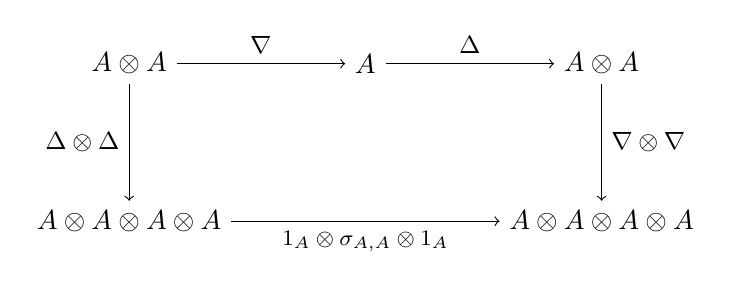
\begin{tikzpicture}
                    \node (AA1) at (0, 0) {$A\otimes A$};
                    \node (A) at (3, 0) {$A$};
                    \node (AA2) at (6, 0) {$A\otimes A$};
                    \node (AAAA1) at (0, -2) {$A\otimes A\otimes A\otimes A$};
                    \node (AAAA2) at (6, -2) {$A\otimes A\otimes A\otimes A$};
                    \draw[->] (AA1) -- node[above]{\small $\nabla$} (A);
                    \draw[->] (A) -- node[above]{\small $\Delta$} (AA2);
                    \draw[->] (AA1) -- node[left]{\small $\Delta\otimes\Delta$} (AAAA1);
                    \draw[->] (AA2) -- node[right]{\small $\nabla\otimes\nabla$} (AAAA2);
                    \draw[->] (AAAA1) -- node[below]{\footnotesize $\mathbbm{1}_A\otimes\sigma_{A,A}\otimes\mathbbm{1}_A$} (AAAA2);
                \end{tikzpicture}
            \end{subfigure}
            \par\bigskip
            \begin{subfigure}[b]{0.3\textwidth}
                \centering
                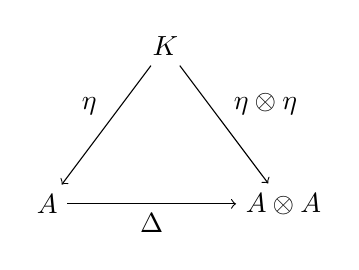
\begin{tikzpicture}
                    \node (K) at (0, 0) {$K$};
                    \node (A) at (-1.5, -2) {$A$};
                    \node (AA) at (1.5, -2) {$A\otimes A$};
                    \draw[->] (K) -- node[above left]{$\eta$} (A);
                    \draw[->] (K) -- node[above right]{$\eta\otimes\eta$} (AA);
                    \draw[->] (A) -- node[below]{$\Delta$} (AA);
                \end{tikzpicture}
            \end{subfigure}
            \begin{subfigure}[b]{0.3\textwidth}
                \centering
                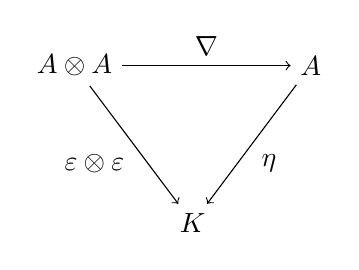
\begin{tikzpicture}
                    \node (K) at (0, -2) {$K$};
                    \node (AA) at (-1.5, 0) {$A\otimes A$};
                    \node (A) at (1.5, 0) {$A$};
                    \draw[<-] (K) -- node[below left]{$\varepsilon\otimes\varepsilon$} (AA);
                    \draw[<-] (K) -- node[below right]{$\eta$} (A);
                    \draw[->] (AA) -- node[above]{$\nabla$} (A);
                \end{tikzpicture}
            \end{subfigure}
            \begin{subfigure}[b]{0.3\textwidth}
                \centering
                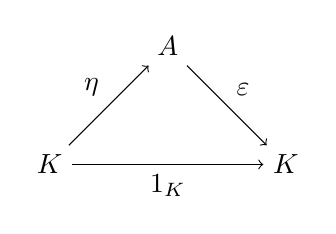
\begin{tikzpicture}
                    \node (A) at (0, 0) {$A$};
                    \node (K1) at (-1.5, -1.5) {$K$};
                    \node (K2) at (1.5, -1.5) {$K$};
                    \draw[->] (K1) -- node[above left]{$\eta$} (A);
                    \draw[->] (A) -- node[above right]{$\varepsilon$} (K2);
                    \draw[->] (K1) -- node[below]{$\mathbbm{1}_K$} (K2);
                \end{tikzpicture}
            \end{subfigure}
            \caption{Bialgebra conditions.}
            \label{fig:bialgebra}
        \end{figure}
    }
    \newdef{Convolution}{\index{convolution}
        Let $(A,\nabla,\eta,\Delta,\varepsilon)$ be a bialgebra. The convolution of two operators $f,g:A\rightarrow A$ is defined as follows:
        \begin{gather}
            f\ast g := \nabla\circ(f\otimes g)\circ\Delta.
        \end{gather}
        When equipped with the convolution as multiplication, the space of operators on a bialgebra also becomes an algebra.
    }

    \newdef{Hopf algebra}{\index{Hopf!algebra}\index{antipode}
        A bialgebra $(A,\nabla,\eta,\Delta,\varepsilon)$ equipped with a linear map $S:A\rightarrow A$ that satisfies
        \begin{gather}
            \nabla\circ(\mathbbm{1}_A\otimes S)\circ\Delta = \nabla\circ(S\otimes\mathbbm{1}_A)\circ\Delta = \eta\circ\varepsilon
        \end{gather}
        or, using the convolution on $A$,
        \begin{gather}
            \mathbbm{1}_A\ast S = S\ast\mathbbm{1}_A = \eta\circ\varepsilon.
        \end{gather}
        The map $S$ is called the \textbf{antipode} or \textbf{coinverse}.
    }
    \remark{Some authors require the antipode to be invertible. (In finite dimensions this is always the case as noted below.)}

    \begin{property}
        Given a Hopf algebra structure on a bialgebra, the antipode $S$ is an antihomomorphism. Furthermore, by noting that it is the inverse of the identity under convolutions, one can show that the antipode is unique (if it exists). Being a Hopf algebra is thus a property, not a structure.
    \end{property}
    \begin{property}[Finite-dimensional bialgebras]
        Any finite-dimensional bialgebra admits an invertible antipode and, in particular, is a Hopf algebra.
    \end{property}

    \newdef{Quasi-triangular Hopf algebra\footnotemark}{\index{R-matrix}\index{quasi-!cocommutative}
        \footnotetext{Sometimes called a \textbf{braided Hopf algebra}.}
        A Hopf algebra $H$ for which there exists an invertible element $R\in H\otimes H$ that satisfies:
        \begin{enumerate}
            \item $R\Delta(a) = \sigma\Big(\Delta(x)\Big)R$,
            \item $(\Delta\otimes\mathbbm{1})(R) = R_{13}R_{23}$, and
            \item $(\mathbbm{1}\otimes\Delta)(R) = R_{13}R_{12}$,
        \end{enumerate}
        where $\sigma(x\otimes y) = y\otimes x$ is the braiding on $H$ and where $R_{ij}\in H\otimes H\otimes H$ is defined using the components of $R$ in the $i^{th}$ and $j^{th}$ position and the unit element $1\in H$ in the other position, i.e. $(a\otimes b)_{13} = a\otimes1\otimes b$.

        The element $R$ is often called the \textbf{universal $R$-matrix}\footnote{This name is in general used for all elements $R\in H\otimes H$ satisfying the first condition above.}. Any Hopf algebra admitting such an element is said to be \textbf{quasi-cocommutative}.
    }

    \begin{example}[Universal enveloping algebra]
        Let $\mathfrak{g}$ be a Lie algebra and consider its universal enveloping algebra $U(\mathfrak{g})$ from Section \ref{section:universal_enveloping_algebra}. This algebra admits a Hopf algebra structure with the following operations:
        \begin{align}
            \Delta(e_i) &:= e_i\otimes1+1\otimes e_i\\
            \varepsilon(e_i) &:= 0\\
            S(e_i) &:= -e_i.
        \end{align}
        It becomes quasi-triangular when equipped with the trivial $R$-matrix $\mathbb{1}_\mathfrak{g}\otimes\mathbb{1}_\mathfrak{g}$.
    \end{example}

    \begin{remark}[Tensor product of modules]\index{Tannaka duality}
        One could ask where bialgebras and especially Hopf algebras naturally arise. Consider an algebra $A$ together with its category of modules $A\mathbf{Mod}$. Now one would like to define a monoidal structure on $A\mathbf{Mod}$ induced by the tensor product on $A$. However, this monoidal structure should be compatible with the action of $A$.

        The intuitive (left) action \[A\otimes(M\otimes_A N)\rightarrow M\otimes_AN: a\otimes m\otimes n\mapsto (am)\otimes n\] does not admit a suitable tensor unit due to its asymmetric definition. To obtain the correct definition, one could be inspired by group representations: $g\cdot(m\otimes n) = gm\otimes gn$. In this case one has the diagonal map $\Delta:G\rightarrow G\times G$ that can be used to act on both sides of the tensor product. One could then ask ``Why not just define the action of an algebra in the same way?'', i.e. \[a\otimes (m\otimes n)\mapsto (am)\otimes(an).\] However, because the action is required to be linear (after all it should be compatible with the algebra morphisms), this definition is not valid. To resolve this issue, the existence of an additional algebra morphism $A\rightarrow A\otimes A$ is required with which one can construct a suitable action as follows:
        \begin{gather}
            A\otimes(M\otimes_AN)\rightarrow M\otimes_AN:a\otimes m\otimes n\mapsto (a_{(1)}m)\otimes(a_{(2)}n).
        \end{gather}
        Together with the usual conditions of an algebra action, one obtains exactly the requirement that $A$ should be a bialgebra. So if $A$ is a bialgebra, then $A\mathbf{Mod}$ will be a monoidal category (this is in fact an equivalence known as \textbf{Tannaka duality}).

        Now, one could require some more structure on $A\mathbf{Mod}$, for example that it admits duals. Consider an $A$-module $V$ together with its dual $V^*\cong\hom(V,\mathbb{C})$. Given a linear map $S:A\rightarrow A$ one could define a general action as follows:
        \begin{gather}
            (af)(v) := f\big(S(a)v\big).
        \end{gather}
        The requirement that this is indeed an action leads to the requirement $S(ab) = S(b)S(a)$ on $S$, which is equivalent to requiring that $S$ is an algebra antihomomorphism. Together with the other compatibility conditions, such as that the evaluation and coevaluation maps induced by the underlying vector spaces are also $A$-module morphisms, one is led to the requirement that $A$ is a Hopf algebra. Hence, if $A$ is a Hopf algebra (with an invertible antipode), then $A\mathbf{Mod}$ will be a rigid monoidal category.

        One could even go further and require the representation category to be braided. This requirement then exactly leads to the Hopf algebra being quasi-triangular (this also explains why these Hopf algebras are sometimes said to be braided).
    \end{remark}

\subsection{Drinfel'd double}

    One can easily generalize Definition \ref{group:bicrossed_product} (when written in terms of group algebras) to the case of bialgebras by replacing the group comultiplication by a general comultiplication:
    \newdef{Bicrossed product of bialgebras}{\index{bicrossed product}
        Two bialgebras $A,B$ are said to form a \textbf{matched pair} (of bialgebras) if there exist actions $-\cdot-:A\otimes B\rightarrow B$ and $-^-:A\otimes B\rightarrow B$, compatible with the coalgebra structures, that satisfy the following equations:
        \begin{enumerate}
            \item $a\cdot(bc) = (a_{(1)}\cdot b_{(1)})(a_{(2)}^{b_{(2)}}\cdot c)$,
            \item $a\cdot1=\varepsilon(a)1$,
            \item $(ab)^c = a^{b_{(1)}\cdot c_{(1)}}b_{(2)}^{c_{(2)}}$,
            \item $1^b = \varepsilon(b)1$, and
            \item $a_{(1)}^{b_{(1)}}\otimes a_{(2)}\cdot b_{(2)} = a_{(2)}^{b_{(2)}}\otimes a_{(1)}\cdot b_{(1)}$.
        \end{enumerate}
        Given such a matched pair, one can define a Hopf algebra structure on $A\otimes B$ defined by the following operations:
        \begin{itemize}
            \item\textbf{Product}: $(a\otimes b)(c\otimes d) = a(b_{(1)}\cdot c_{(1)})\otimes b_{(2)}^{c_{(2)}}d$,
            \item\textbf{Coproduct}: $\Delta(a\otimes b) = (a_{(1)}\otimes b_{(1)})\otimes(a_{(2)}\otimes b_{(2)})$, and
            \item\textbf{Counit}: $\varepsilon(a\otimes b) = \varepsilon_A(a)\varepsilon_B(b)$.
        \end{itemize}
        If the bialgebras are equipped with antipodes, the bicrossed product admits an induced antipode:
        \begin{gather}
            S(a\otimes b) = S_B(b_{(2)})\cdot S_A(a_{(2)})\otimes S_B(b_{(1)})^{S_A(a_{(1)})}.
        \end{gather}
    }

    \begin{example}[Tensor product]
        In the case where the bialgebra actions are given by left multiplication with the counits, the bicrossed product is isomorphic to the tensor product.
    \end{example}

    \begin{construct}[Drinfel'd double\footnotemark]\index{Drinfel'd!quantum double}
        \footnotetext{Also known as the \textbf{quantum double} (especially in physics).}
        Consider a Hopf algebra $H$ (with invertible antipode). It can be shown that $H$ and $(H^{op})^*$ form a matched pair of bialgebras. The left and right actions are induced by pullback:
        \begin{align}
            (a\cdot f)(b) &= f\big(S^{-1}(a_{(2)})ba_{(1)}\big)\\
            a^f &= f\big(S^{-1}(a_{(3)})a_{(1)}\big)a_{(2)}
        \end{align}
        The resulting bicrossed product $(H^{op})^*\bowtie H$ is called the Drinfel'd double $D(H)$.
    \end{construct}
    \begin{example}[Drinfel'd double for groups]
        Consider a finite group $G$ together with its associated group algebra $\mathbb{C}[G]$. On this algebra one can put a Hopf algebra structure as follows:
        \begin{align}
            \Delta(g) &= g\otimes g,\\
            \varepsilon(g) &= 1.
        \end{align}
        On the other hand one can also put a Hopf algebra structure on the dual $\mathbb{C}[G]^*$:
        \begin{align}
            \Delta(P_g) &= \sum_{hh'=g}P_h\otimes P_{h'},\\
            \varepsilon(P_g) &= \delta_{g,e},
        \end{align}
        where the basis for $\mathbb{C}[G]^*$ is given by the ``projections'' $P_g:h\mapsto\delta_{g,h}$. Antipodes for both algebras are given by $S(g)=g^{-1}$ and $S(P_g) = P_{g^{-1}}$.

        ?? COMPLETE ??
    \end{example}

\section{Quantum groups}

    This section heavily builds upon the theory presented in Chapter \ref{chapter:lie}. The content is partially based on talks by \textit{Andr\'e Henriques}.

    \begin{construct}[Jimbo-Drinfeld]\index{Jimbo-Drinfeld}
        Consider a Lie algebra $\mathfrak{g}$ together with its universal enveloping algebra $U(\mathfrak{g})$ constructed using the Chevalley-Serre relations \ref{lie:enveloping_algebra_construct}:
        \begin{enumerate}
            \item $[H_i,H_j] = 0$,
            \item $[H_i,E_j] = a_{ij}E_j$,
            \item $[H_i,F_j] = -a_{ij}F_j$,
            \item $[E_i,F_j] = \delta_{ij}H_j$,
            \item $\text{ad}_{E_i}^{|a_{ij}|-1}(E_j) = 0$, and
            \item $\text{ad}_{F_i}^{|a_{ij}|-1}(F_j) = 0$.
        \end{enumerate}
         To obtain the quantum group $U_q(\mathfrak{g})$, which is also called a \textbf{deformation} or \textbf{quantization} of $U(\mathfrak{g})$, one replaces the generators $H_i$ by the following generators\footnote{To be complete one should also add generators $K_i^{-1}$ that act formally as inverses of the generators $K_i$.}:
        \begin{gather}
            K_i := q^{d_iH_i},
        \end{gather}
        where $d_i := \frac{\langle\alpha_i,\alpha_i\rangle}{2}$ is related to the norm of the $i^{th}$ simple root. So, instead of the $H_i$ being functionals on the root lattice, one gets functions from the root lattice to the Laurent polynomials in $q$, i.e. to $\mathbb{C}[q,q^{-1}]$.

        From this functional point of view one can rewrite the second and third relation as follows:
        \begin{align*}
            f\cdot E_i &= E_i\tau_{\alpha_i}(f),\\
            f\cdot F_i &= F_i\tau_{-\alpha_i}(f),
        \end{align*}
        where $f$ is a polynomial in the $H_i$'s and $\tau_{\alpha_i}(f)(\lambda) := f(\lambda+\alpha_i)$. Replacing $H_i$ by $K_i$ one obtains the following relations:
        \begin{enumerate}
            \item[$2^*.$] $K_iE_j = q^{d_ia_{ij}}E_jK_i$, and
            \item[$3^*.$] $K_iF_j = q^{-d_ia_{ij}}F_jK_i$.
        \end{enumerate}
        The three relations between the $E_i$'s and the $F_i$'s are deformed using $q$-analog numbers. First, define the $q$-numbers\footnote{Note that $q$-numbers are often defined differently. This definition is equal to $\frac{1}{q^{n-1}}[n]_{q^2}$ when rewritten using the common definition.}:
        \begin{gather}
            [n]_q := \frac{q^n - q^{-n}}{q - q^{-1}}.
        \end{gather}
        Using this definition Serre relation 4 becomes
        \begin{enumerate}
            \item[$4^*.$] $[E_i,F_j] = \delta_{ij}[H_i]_{q^{d_i}} = \delta_{ij}\frac{K_i - K_i^{-1}}{q^{d_i} - q^{-d_i}}$,
        \end{enumerate}
        where the factor $[H_i]_{q^{d_i}}$ should be interpreted as first evaluating $H_i$ on a root and then taking the $q$-analog. The adjoint action relations (5 and 6) on $E_i$ and $F_i$ can be rewritten by replacing binomial coefficients by their $q$-analogs ($i\neq j$):
        \begin{enumerate}
            \item[$5^*.$] $\sum_{k=1}^{1+|a_{ij}|} (-1)^k\begin{bmatrix}1+|a_{ij}|\\k\end{bmatrix}_{q^{d_i}}E_i^{1+|a_{ij}|-k}E_jE_i^k = 0$, and
            \item[$6^*.$] $\sum_{k=1}^{1+|a_{ij}|} (-1)^k\begin{bmatrix}1+|a_{ij}|\\k\end{bmatrix}_{q^{d_i}}F_i^{1+|a_{ij}|-k}F_jF_i^k = 0$.
        \end{enumerate}
    \end{construct}

\section{Differential structures}
\subsection{Differential calculi}

    \newdef{First-order differential calculus}{\index{differential}\index{calculus}\index{differentiable}\label{qa:fodc}
        Let $A$ be an associative algebra and let $\Gamma$ be an $A$-bimodule. Together with an $A$-bimodule morphism $d:A\rightarrow\Gamma$ this structure is called a first-order differential calculus (FODC) if it satisfies the following two conditions:
        \begin{enumerate}
            \item\textbf{Leibniz rule}: $d(ab) = (da)b + a(db)$.
            \item\textbf{Standard form}: Every element $g\in\Gamma$ can be written as \[g = \sum_{i=1}^na_i(db_i)\]
            for some $n\in\mathbb{N}$ and (not necessarily unique) elements $\{a_i,b_i\}_{i\leq n}$.
        \end{enumerate}
        If $\ker(d)\cong K$, where $K$ is the underlying field, the calculus is said to be \textbf{connected}. A calculus is said to be \textbf{inner} if the differential $d$ acts through a commutator, i.e. there exists an element $\theta\in A$ such that $da=[\theta,a]$ for all $a\in A$.

        An algebra morphism $\phi:A\rightarrow B$ is said to be \textbf{differentiable}, with respect to a choice of FODCs on $A$ and $B$, if there exists an $A$-bimodule morphism $\phi_*:\Gamma_A\rightarrow\Gamma_B$ ($A$ inherits an action on $\Gamma_B$ through $\phi$) such that $d\circ\phi=\phi_*\circ d$. If such a morphism exists, it is given by $\phi_*(adb)=\phi(a)d\phi(b)$.
    }
    \remark{The second condition can be rewritten in terms of a right action using the Leibniz rule.}

    \newdef{Cotangent dimension}{\index{dimension!cotangent}\index{parallelizable}
        If $\Gamma$ is free over $A$ with a basis of cardinality $n$, it is said to be \textbf{parallelized with cotangent dimension} $\dim(A)-1$.

        This is in analogy with the case of function algebras $C^\infty(M)$ and the first de Rham space $\Omega^1(M)$ on a smooth manifold. If $\Omega^1(M)$ is free over $C^\infty(M)$, this implies that there exists a global basis of one-forms or, equivalently, a global frame of the tangent bundle. This is the same as saying that $M$ is parallelizable. (The cotangent dimension will be explained later.)
    }

    \begin{example}[Universal FODC]
        Consider an algebra $A$ with multiplication $\mu$. The bimodule $\Omega_\mathrm{uni}:=\ker(\mu)$, equipped with the operator $da:=1\otimes a-a\otimes1$, defines a first-order differential calculus on $A$. Furthermore, every FODC over $A$ can be obtained as the quotient $\Omega_\mathrm{uni}/\mathcal{N}$ for a subbimodule $\mathcal{N}$. The universal FODC is inner if and only if there exists a central element $F\in A\otimes A$ such that $\mu(F)=1$.
    \end{example}
    \begin{example}[K\"ahler differentials]\index{K\"ahler!differential}
        In commutative algebra one has an equivalent construction. There one takes the module $\Omega^1(A)$ to be the quotient $I/I^2$, where $I$ is the again the augmentation ideal $I:=\ker(\mu)$. The quotient enforces that the bimodule is symmetric and, hence, that the Leibniz rule becomes
        \begin{gather}
            d(ab) = adb + bda.
        \end{gather}
        The module of K\"ahler differentials plays the same role as the universal FODC in commutative algebra in that it is universal with respect to modules over commutative algebras equipped with a derivation.
    \end{example}

    \newdef{Differential calculus}{\index{calculus}\index{exterior!algebra}
        Consider an algebra $A$. A differential calculus over $A$ is an $A$-bimodule with the structure of differential graded algebra $(\Gamma^\bullet,d)$ such that $\Gamma^0=A$. If $\Gamma^\bullet$ is freely generated by $A$ and $dA$, then $(\Gamma^\bullet,d)$ is often called an \textbf{exterior algebra} over $A$.
    }

    \begin{property}[Prolongation]\label{qa:prolongation}
        Every FODC $(\Gamma,d)$ admits a maximal extension (or \textbf{prolongation}) to an exterior algebra. In degree $k$ it is obtained by taking
        \begin{gather}
            \Gamma^k := \underbrace{\Gamma\otimes_A\cdots\otimes_A\Gamma}_{k\text{ times}},
        \end{gather}
        and modding out the ideal generated by the following relations:
        \begin{gather}
            \left\{\sum_ida_i\otimes db_i+du_i\otimes dv_i=0\,\middle\vert\,\sum_ia_idb_i=\sum_i(du_i)v_i\right\}.
        \end{gather}
        If one starts from the universal FODC over an algebra, the resulting differential calculus is again universal in the sense that all other differential calculi can be obtained by taking quotients by differential ideals.
    \end{property}

\subsection{Covariance}

    \newdef{Covariant FODC}{
        An FODC $(\Gamma,d)$ over a Hopf algebra $H$ is said to be left-covariant if it is a left $H$-comodule such that
        \begin{gather}
            \Phi(adb) = \Delta(a)(\mathbbm{1}_H\otimes d)\Delta(b).
        \end{gather}
    }

% \part{(Differential) Geometry}\label{part:diffgeom}
% \insertparttoc

% \chapter{Elementary Geometry}

\minitoc

\section{Euclidean geometry}
\subsection{Postulates}

    \begin{axiom}
        Between every two points, one can draw a straight line.
    \end{axiom}

    \begin{axiom}
        Every (finite) line segment can be extended to a straight line.
    \end{axiom}

    \begin{axiom}
        Given any point and any (nonnegative) distance, one can draw a circle with the given point as centre and distance as radius.
    \end{axiom}

    \begin{axiom}
        All right angles are congruent.
    \end{axiom}

    \begin{axiom}[Parallel postulate]
        Consider a straight line intersecting two other straight lines as in \cref{fig:parallel_postulate}. If the sum of the interior angles ($\hat{A}$ and $\hat{B}$) on one side is less than $180^\circ$ (2 right angles), the two straight lines will intersect on that side (if extended indefinitely).
    \end{axiom}

    \begin{figure}[t!]
        \centering
        \begin{tikzpicture}
            \draw (0, 5) -- (10, 2);
            \draw (0, -3) -- (10, 1);
            \draw (3, 5) -- (2, -3);
            \node at (3.2, 3.7) {$\hat{A}$};
            \node at (2.5, -1.6) {$\hat{B}$};
        \end{tikzpicture}
        \caption{Parallel postulate.}
        \label{fig:parallel_postulate}
    \end{figure}

    \begin{result}
        If the sum of the interior angles on side (and, hence, on both sides) is exactly $180^\circ$, i.e.~they are supplementary, the two straight lines are parallel. (This is the reason for the name of the axiom.)
    \end{result}

    \begin{property}[Alternate interior angles]\index{interior!angles}
        Consider a straight line intersecting two parallel lines as follows:
        \begin{gather*}
            \begin{tikzpicture}
                \node (A) at (0, 0) {};
                \node (D) at (8, -3) {};
                \node (P) at (3, -3) {};
                \node (Q) at (5, 0) {};
                \draw (A) -- (8, 0);
                \draw (0, -3) -- (D);
                \draw (2, -4.5) -- (6, 1.5);
                \draw pic[draw, angle radius = .5cm] {angle =D--P--Q};
                \draw pic[draw, angle radius = .5cm] {angle =A--Q--P};
                \node at (4, -2.4) {$\alpha$};
                \node at (4, -.5) {$\beta$};
            \end{tikzpicture}
        \end{gather*}
        The parallel postulate implies that the angles $\alpha$ and $\beta$, called alternate interior angles, are equal.
    \end{property}

\subsection{Triangles and quadrangles}

    \begin{method}[Congruent triangles]
        Two triangles are congruent when they satisfy one and, hence, all of the following equivalent conditions:
        \begin{enumerate}[\quad a)]
            \item SSS (side--side--side): The triangles have corresponding sides of equal length.
            \item SAS (side--angle-side): The triangles have two corresponding pairs of sides of equal length and the included angles are of equal size.
            \item ASA (angle--side--angle): The triangles have two corresponding pairs of equal angles and the included sides are of equal length.
        \end{enumerate}
    \end{method}
    \begin{result}
        In right triangles, by \textit{Pythagoras' theorem} (see \cref{geom:pythagoras} below), the SSS condition gives rise to another possibility. The RHS (right-angle--hypotenuse--side) condition says that two right triangles are congruent if and only if
        \begin{enumerate}
            \item their \textbf{hypotenuses}, i.e.~the sides opposite to the right angle, are of equal length, and
            \item they have a pair of corresponding sides of equal length.
        \end{enumerate}
    \end{result}

    \begin{theorem}[Thales]\index{Thales}
        Consider \cref{fig:thales}. The ratios of sides in the triangles $\bigtriangleup ABC$ and $\bigtriangleup PQC$ are equal:
        \begin{gather}
            \frac{|PQ|}{|AB|} = \frac{|PC|}{|AC|} = \frac{|QC|}{|BC|}\,.
        \end{gather}
    \end{theorem}

    \begin{figure}
        \centering
        \begin{tikzpicture}
            \node (A) at (0, 0) {};
            \node (B) at (10, 2) {};
            \node (C) at (5, 8) {};
            \node (P) at (2, 3.2) {};
            \node (Q) at (8, 4.4) {};
            \draw (A.center) node[left]{$A$} -- (B.center) node[right]{$B$} -- (C.center) node[above]{$C$}-- (A.center);
            \draw (P.center) node[left]{$P$} -- (Q.center) node[right]{$Q$};
            \draw pic[draw, angle radius = 1cm] {angle =B--A--C};
            \draw pic[draw, angle radius = .9cm] {angle =B--A--C};
            \draw pic[draw, angle radius = 1cm] {angle =C--B--A};
            \draw pic[draw, angle radius = 1cm] {angle =Q--P--C};
            \draw pic[draw, angle radius = .9cm] {angle =Q--P--C};
            \draw pic[draw, angle radius = 1cm] {angle =C--Q--P};
        \end{tikzpicture}
        \caption{Thales' theorem.}
        \label{fig:thales}
    \end{figure}

    \begin{theorem}[Characteristics of parallelograms]\index{parallelogram}
        A quadrangle is a parallellogram if and only if one and, hence, all of the following equivalent conditions hold:\footnote{The first condition is usually taken as the definition.}
        \begin{enumerate}
            \item opposite sides are parallel,
            \item opposite sides are of equal length,
            \item opposite corners are of equal size, or
            \item diagonals bisect.
        \end{enumerate}
    \end{theorem}

\section{Trigonometry}

    \begin{figure}[ht!]
        \centering
        \begin{tikzpicture}
            \node (A) at (0, 0) {};
            \node (B) at (10, 0) {};
            \node (C) at (10, 5) {};
            \draw (A.center) -- node[below]{$b$} (B.center) -- node[right]{$a$} (C.center) -- node[above]{$c$} (A.center) pic["$\alpha$", draw, angle radius = 1.5cm] {angle = B--A--C} pic["$\gamma$", draw, angle radius = 1cm] {angle = C--B--A} pic["$\beta$", draw, angle radius = 1cm] {angle = A--C--B};
        \end{tikzpicture}
        \caption{Right-angled triangle.}
        \label{fig:general_triangle}
    \end{figure}

    \newdef{Trigonometric functions}{\index{sine}\index{cosine}\index{tangent}\index{hypotenuse}
        Consider a triangle as in \cref{fig:general_triangle}, where $\gamma=\tfrac{\pi}{2}$.
        \begin{align}
            \sin(\alpha) &:= \frac{a}{c}\\
            \cos(\alpha) &:= \frac{b}{c}\\
            \tan(\alpha) &:= \frac{a}{b}
        \end{align}
        The longest side, $c$ in this case, always corresponds to the hypotenuse.
    }
    \begin{result}
        Since the adjacent side for one angle is the opposite side for the other, the formulas above give rise to the following relations:
        \begin{align}
            \sin(\alpha) &= \cos(\tfrac{\pi}{2}-\alpha)\,,\\
            \cos(\alpha) &= \sin(\tfrac{\pi}{2}-\alpha)\,,\\
            \tan(\alpha) &= \frac{1}{\tan(\tfrac{\pi}{2}-\alpha)}\,.
        \end{align}
    \end{result}
    
    \begin{notation}[Cotangent]\index{cotangent}
        Because it occurs relatively often, the last expression above receives a distinct notation:
        \begin{gather}
            \cot(\alpha) := \frac{1}{\tan(\alpha)}\,.
        \end{gather}
    \end{notation}
    Lesser known trigonometric functions are the cotangent-like versions of the sine and cosine.
    \newnot{Secant}{\index{secant}
        \begin{align}
            \sec(\theta) &:= \frac{1}{\sin(\theta)}\\
            \csc(\theta) &:= \frac{1}{\cos(\theta)}
        \end{align}
    }

    \begin{formula}
        \begin{gather}
            \tan(\theta)=\frac{\sin(\theta)}{\cos(\theta)}
        \end{gather}
        for any angle $\theta\in[0,2\pi[$.
    \end{formula}

    \begin{theorem}[Pythagoras]\index{Pythagoras}\label{geom:pythagoras}
        In any right-angled triangle, where $c$ denotes the hypotenuse, the following relation between the sides holds:
        \begin{gather*}
            a^2 + b^2 = c^2\,.
        \end{gather*}
    \end{theorem}
    Using the definitions of the trigonometric functions, this can also be rewritten.
    \begin{theorem}[Fundamental theorem of trigonometry]\index{fundamental theorem!of trigonometry}
        \begin{gather}
            \sin^2(\theta)+\cos^2(\theta)=1
        \end{gather}
        for any angle $\theta\in[0,2\pi[$.
    \end{theorem}

    The Pythagorean theorem can be extended as follows.
    \begin{formula}[Cosine law]
        In a general triangle, sides and angles are related as follows:
        \begin{gather}
            a^2+b^2-2ab\cos(\gamma) = c^2\,.
        \end{gather}
    \end{formula}

    \begin{formula}[Sine law]
        In a general triangle, sides and sines of the opposite angles are related as follows:
        \begin{gather}
            \frac{\sin(\alpha)}{a} = \frac{\sin(\beta)}{b} = \frac{\sin(\gamma)}{c}
        \end{gather}
    \end{formula}

    \begin{formula}[Tangent law]
        \begin{gather}
            \frac{a+b}{a-b} = \frac{\tan\bigl(\tfrac{1}{2}(\alpha+\beta)\bigr)}{\tan\bigl(\tfrac{1}{2}(\alpha-\beta)\bigr)}
        \end{gather}
    \end{formula}

    \begin{formula}[Addition formulas]
        \begin{align}
            \sin(\alpha+\beta) &= \sin(\alpha)\cos(\beta)+\cos(\alpha)\sin(\beta)\\
            \cos(a+b) &= \cos(\alpha)\cos(\beta)-\sin(\alpha)\sin(\beta)\\
            \tan(\alpha+\beta) &= \frac{\tan(\alpha)+\tan(\beta)}{1+\tan(\alpha)\tan(\beta)}
        \end{align}
    \end{formula}

    Besides the addition formulas, there are also product formulas. (Only one is given, since the others can be derived from it.)
    \begin{result}[Werner--Simpson]\index{Werner--Simpson formulas}
        \begin{gather}
            2\sin(\alpha)\cos(\beta) = \sin(\alpha-\beta)+\sin(\alpha+\beta)
        \end{gather}
    \end{result}
% \input{Math/Geometry/Curves}
% \chapter{Manifolds}\label{chapter:manifolds}

References for this chapter (and \ref{part:diffgeom} in general) are \cite{AMP1, AMP2, diffgeom_physics, kms, sen_nash, schuller}.

\section{Charts}

    \newdef{Chart}{\index{chart}\label{diff:chart}
        Consider a topological space  $M$. Let $U$ be an open subset of $M$ and let $O$ be an open subset of $\mathbb{R}^n$ such that there exists a homeomorphism $\varphi:U\rightarrow O$. The pair $(U,\varphi)$ is called a chart on $M$.
    }
    \newdef{Transition map}{
        Let $(U_1,\varphi_1)$ and $(U_2,\varphi_2)$ be two charts on $M$. The mapping $\varphi_1^{-1}\circ\varphi_2$, defined on the intersection $U_1\cap U_2$, is called the transition map between the charts.

        If $\varphi_1^{-1}\circ\varphi_2$ is continuous, the charts are said to be $C^0$-compatible. However, because the composition of any two continuous functions is also continuous, every two charts on a topological space are $C^0$-compatible.
    }

    \newdef{Atlas}{\index{atlas}
        Let $M$ be a topological space and let $\{(U_i,\varphi_i)\}_{i}$ be a collection of pairwise compatible charts covering $M$. This collection of charts is called an atlas on $M$. From the above remark on $C^0$-compatibility it follows that every atlas is a $C^0$-atlas. Depending on the type of compatibility condition that was used, one can define different types of atlases.
    }
    \newdef{Maximal atlas}{
        Let $\mathcal{A}_1$ and $\mathcal{A}_2$ be two atlases on the same topological space $M$. If $\mathcal{A}_1\cup\mathcal{A}_2=\mathcal{A}$ is again an atlas, then the atlases are said to be equivalent or compatible. The largest such union is called a maximal atlas.
    }

    \newdef{Manifold}{\index{manifold}
        A topological space $M$ equipped with a maximal $C^0$-atlas $\mathcal{A}$ is called a \textbf{topological} manifold. An alternative definition (often used in topology) is that of a locally Euclidean Hausdorff space. The topology on $M$ is generated by the collection of charts.
    }
    \begin{remark*}\index{smooth!manifold}\index{PL manifold}
        \nomenclature[S_Man]{$\textbf{Man}^p$}{category of $C^p$-manifolds}
        \nomenclature[S_Diff]{$\textbf{Diff}$}{category of smooth manifolds}
        In the literature second-countability is often added to the definition of a topological manifold. This ensures that the space has (among others) the property of paracompactness \ref{topology:paracompact} and hence lends itself to the construction of partitions of unity (necessary for the introduction of integration theory as in chapter \ref{section:integration_manifolds}).

        For an alternative definition of manifolds in the context of \textit{smooth spaces} see section \ref{section:smooth_spaces}.

        If all transition maps are $C^k$-diffeomorphisms, the manifold is called a $C^k$-manifold. A $C^\infty$-manifold is also called a \textbf{smooth manifold}. If the transition maps are not only smooth, but even analytic \ref{calculus:analytic}, then the manifold is called an \textbf{analytic} or $C^\omega$-manifold. A topological manifold equipped with a maximal atlas for which the transition maps are piecewise linear is called a \textbf{PL manifold}.
    \end{remark*}

    \newdef{\difficult{Structure sheaf}}{\index{structure!sheaf}
        Let $M$ be a $C^k$-manifold. The structure sheaf $\mathcal{O}_M$ is defined as the sheaf (see definition \ref{sheaf:def}) that assigns to every open set $U\subseteq M$ the set of $C^k$-functions $f:U\rightarrow\mathbb{R}$.

        Generally, one can define for all $j\leq k$ the sheaf $\mathcal{O}^j_M$ as the sheaf that assigns to every open set $U\subseteq M$ the set of $C^j$-functions $f:U\rightarrow\mathbb{R}$.

        From the ''sheafy'' point of view one can equivalently define a smooth manifold as a ringed space that is locally isomorphic to $\mathbb{R}^n$ equipped with its standard space of differentiable functions. (This is an extension of the constructions in algebraic geometry as given in sections \ref{section:varieties} and \ref{section:schemes}.)
    }

    \begin{theorem}[Whitney]\index{Whitney}
        Every $C^k$-atlas contains a $C^\infty$-atlas (at least on paracompact manifold). Furthermore, two $C^k$-atlases are equal if and only if they contain the same $C^\infty$-atlas. It follows that every differentiable manifold is automatically smooth.
    \end{theorem}

    \begin{theorem}[Rad\'o-Moise]\index{Rad\'o-Moise}\label{diff:rado_moise}
        In dimensions $1,2$ and $3$ there exists for every topological manifold a unique smooth structure.
    \end{theorem}
    \begin{theorem}
        For dimensions higher than $4$ there exist only finitely many distinct smooth structures on compact manifolds. In fact, for \textit{PL} manifolds the number of smooth structures is fixed for each dimension (except for $4$).
    \end{theorem}
    \sremark{In $\dim M = 4$ there exist only partial results. For noncompact manifolds there exist uncountably many distinct smooth structures. For compact manifolds there exists no complete characterization.}

    \newdef{Smooth function}{\index{smooth!function}\index{local!representation}\label{manifolds:smooth_function}
        Let $f:M\rightarrow N$ be a function between two smooth manifolds. $f$ is said to be smooth if there exist charts $(U,\varphi)$ and $(V,\psi)$ for $M$ and $N$ with $f(U)\subseteq V$ such that the function
        \begin{gather}
            \label{diff:local_representation}
            f_{\varphi\psi} = \psi\circ f\circ\varphi^{-1}
        \end{gather}
        is smooth on $\mathbb{R}^n$. This function is said to be the \textbf{local representation} of $f$.
    }
    \begin{example}[Smooth curve]\index{curve}\label{diff:curve}
        A smooth function $\gamma:\mathbb{R}\rightarrow M$ with $\gamma(0)=p$ is called a smooth curve through $p\in M$.
    \end{example}

    \begin{notation}
        \nomenclature[S_Cinfty]{$C^\infty_p(M)$}{ring of smooth functions $f:M\rightarrow\mathbb{R}$ on a neighbourhood of $p\in M$}
        The set of all $C^\infty$-functions on a manifold $M$, defined on a neighbourhood of $p\in M$, is denoted by $C^\infty_p(M)$. This set forms a commutative ring when equipped with the usual sum and product (composition) of functions.
    \end{notation}

    \remark{Depending on the choice of chart one can define other types of functions in the same way, e.g. $C^k$-functions or piecewise linear functions.}

    \newdef{Good cover\footnotemark}{\index{cover}\index{finite!type}\label{diff:good_cover}
        \footnotetext{Sometimes called a \textbf{nice cover}.}
        Let $M$ be an $n$-dimensional manifold with an open cover $\mathcal{U}=\{U_i\}_{i\in I}$. The cover $\mathcal{U}$ is called a good cover if every nonempty finite intersection $U_{i_1}\cap\ldots\cap\,U_{i_k}$ is contractible. (Many authors require the intersections to be diffeomorphic to $\mathbb{R}^n$. This is also called a \textbf{differentiable good cover}.)

        If a manifold admits a finite good cover, it is said to be of \textbf{finite type}.
    }

    \begin{property}
        Every paracompact smooth manifold admits a (differentiable) good cover. Furthermore, if the manifold is compact, it admits a finite good cover.
    \end{property}

\section{Tangent vectors}\label{section:tangent_space}

    \newdef{Tangent vector}{\index{tangent!vector}\index{derivation}\label{diff:derivation}
        Let $M$ be a smooth manifold and consider a point $p\in M$. A tangent vector to $M$ at $p$ is a differential operator, i.e. a map $v_p:C^\infty_p(M)\rightarrow\mathbb{R}$ satisfying the properties
        \begin{enumerate}
            \item \textbf{Linearity}: $v_p(af+g) = av_p(f) + v_p(g)$, and
            \item \textbf{Leibniz property}: $v_p(fg) = f(p)v_p(g) + g(p)v_p(f)$
        \end{enumerate}
        for all $f,g:\in C^\infty_p(M)$ and $a\in\mathbb{R}$. Maps with these properties are also called \textbf{derivations}\footnote{More generally, every operation that satisfies the Leibniz property is called a derivation.}.
    }
    \begin{property}
        For every constant function $c:p\mapsto c$ one finds that
        \begin{gather}
            v_p(c)=0.
        \end{gather}
    \end{property}

    \newdef{Tangent space}{\index{tangent!space}\index{basis}\label{diff:tangent_vector_partial}
        Using the previous definition one can construct a tangent (vector) space $T_pM$ at each point $p\in M$. The basis vectors are given by
        \begin{gather}
            \left.\ds\pderiv{}{q^i}\right|_{p}:C^\infty_p(M)\rightarrow\mathbb{R}:f\mapsto \pderiv{}{q^i}\left(f\circ\varphi^{-1}\right)(\varphi(p))
        \end{gather}
        where $(U, \varphi)$ is a coordinate chart such that $p\in U$ with local coordinates $(q^1,\ldots,q^n)$.
    }
    Due to the explicit dependence of the tangent vectors on the point $p\in M$, it is clear that for curved manifolds the tangent spaces belonging to different points are not the same. However, they are related through the following property:
    \begin{property}
        From the above construction it follows that
        \begin{gather}
            \dim(T_p M)=\dim(M)
        \end{gather}
        for all $p\in M$. Theorem \ref{linalgebra:dimension_isomorphism} then implies that the tangent spaces over two distinct points $p,q\in M$ are isomorphic. A way to relate distinct tangent spaces will be presented in sections \ref{section:linear_connections} and \ref{section:covariant_derivatives}.
    \end{property}

    \newadef{Tangent space $\dag$}{\label{diff:alternative_definition}
        Let $(U,\varphi)$ be a chart around the point $p\in M$. Two smooth curves $\gamma_1,\gamma_2$ through $p\in M$ are said to be tangent at $p$ if
        \begin{gather}
            \label{diff:equal_derivative}
            \deriv{(\varphi\circ\gamma_1)}{t}(0) = \deriv{(\varphi\circ\gamma_2)}{t}(0),
        \end{gather}
        or, equivalently, if their local representations are tangent at 0. This defines an equivalence relation\footnote{The relation is well-defined because the transition maps (and their Jacobian matrices) are invertible and thus nonsingular.} on the set of smooth curves through $p$. The tangent space at $p$ is then defined as the set of equivalence classes of tangent curves through $p$. These equivalence classes can be explicitly constructed as follows:

        The tangent vector to the curve $c(t)$ through $p$ is defined by the following formula:
        \begin{gather}
            v_p(f) = \left.\deriv{(f\circ c)}{t}\right|_{t=0}.
        \end{gather}
        Applying the chain rule gives
        \begin{gather}
            \label{diff:tangent_vector_chain_rule}
            v_p(f) = \pderiv{(f\circ\varphi^{-1})}{q^i}(\varphi(p))\deriv{q^i}{t}(0)
        \end{gather}
        where $q^i=(\varphi\circ c)^i$. The first factor depends only on the point $p$ while the second factor is equal for all tangent curves through $p$. It is thus clear that curves satisfying equation \ref{diff:equal_derivative} define the same tangent vector.
    }

\section{Submanifolds}
\subsection{Immersions and submersions}

    In this section the tangent map induced by a smooth function $f:M\rightarrow N$ is denoted by $T_pf:T_pM\rightarrow T_{f(p)}N$. A formal definition is given in equation \ref{diff:T_function} when enough mathematical background has been introduced. For now this will be the map that is locally represented by the Jacobian of $f$.

    \newdef{Immersion}{\index{immersion}
        Let $f:M\rightarrow N$ be a differentiable function between smooth manifolds. It is called an immersion if its derivative is everywhere injective, or equivalently, if its derivative has maximal rank everywhere:
        \begin{gather}
            \text{rk}(T_pf)=\dim(M)\qquad\qquad\forall p\in M.
        \end{gather}
    }

    \newdef{Critical point}{\index{critical!point}\label{diff:nondegenerate_critical_point}
        A point $p\in\dom(f)$ is said to be critical if the rank of the Jacobian $T_pf$ is not maximal. The image of a critical point is called a \textbf{critical value}.

        At a critical point $p\in M$ the Hessian of $f$ gives a well-defined quadratic form. A critical point is said to be \textbf{nondegenerate} if the Hessian is nonsingular there.
    }
    \begin{property}[Criticality]\label{diff:critical_point}
        A point $p\in\dom(f)$ is critical if and only if there exists a chart $(U,\varphi)$ containing $p$ for which $\pderiv{f}{x^i}(p)=0$.
    \end{property}
    \begin{theorem}[Sard]\index{Sard}
        Consider a map $\psi:M\rightarrow N$, where $\dim M=m$ and $\dim N=n$ and let $k_0 = \max\{1, m-n+1\}$. If $\psi$ is of class $C^k$, with $k\geq k_0$, the set of critical values of $\psi$ has Lebesgue measure 0.
    \end{theorem}

    \newdef{Regular point}{
        A regular point of $f$ is a point $p\in M$ such that $T_pf$ is surjective.
    }
    \newdef{Regular value}{\index{regular!value}
        Let $f:M\rightarrow N$ be a differentiable map between smooth manifolds. A point $y\in N$ is called a \textbf{regular value} if every point in the preimage $f^{-1}(y)$ is a regular point or, equivalently, if it is not a critical value.
    }

    \begin{result}\label{diff:regular_point}
        It follows from property \ref{diff:critical_point} that a point $p\in\dom(f)$ is regular if and only if $\pderiv{f}{x^i}(p)\neq0$ in all charts $(U,\varphi)$ containing $p$.
    \end{result}

    \newdef{Submersion}{\index{submersion}\label{diff:submersion}
        Let $f:M\rightarrow N$ be a differentiable map between smooth manifolds. It is called a submersion if all $p\in M$ are regular, or equivalently, if
        \begin{gather}
            \text{rk}(T_pf)=\dim(N)
        \end{gather}
        for all $p\in M$.
    }

    \newdef{Embedding}{\index{embedding}
        A differentiable map between smooth manifolds is called a smooth embedding if it is both an immersion and an embedding in the topological sense \ref{topology:embedding}. This implies that the submanifold topology coincides with the subspace topology \ref{topology:relative_topology}.
    }

\subsection{Submanifolds}

    \newdef{Submanifold}{\index{sub!manifold}
        Let $M$ be a manifold. A subset $N\subset M$ is called a submanifold of $M$ if $N$, equipped with the subspace topology, is a topological manifold on its own.
    }
    \newdef{Embedded submanifold}{
        Let $M$ be a manifold. A smooth manifold $N$ is called an embedded or \textbf{regular submanifold} (of $M$) if there exists an embedding $f:M\hookrightarrow N$.
    }

    \newdef{Slice}{\index{slice}
        Consider two positive integers $m<n$. The space $\mathbb{R}^m$ can be canonically identified with a subspace of $\mathbb{R}^n$ as follows:
        \begin{gather}
            \mathbb{R}^m\cong\mathbb{R}^m\times\{0,\ldots, 0\}\overset{\iota}{\hookrightarrow}\mathbb{R}^m\times\mathbb{R}^{n-m}\cong\mathbb{R}^n
        \end{gather}
        where $\iota:(x_1,\ldots,x_m)\mapsto(x_1,\ldots,x_m,0,\ldots,0)$ is the canonical inclusion map. Subspaces obtained by setting a number of coordinates equal to 0 (or any other constant) are called slices.
    }
    \begin{adefinition}[Embedded submanifold]
        A $k$-dimensional embedded manifold $N$ of $M$ can be defined equivalently as a subset of $M$ such that there exists a positive integer $k$ and such that for every point $p\in N$ there exists a chart $(U,\varphi)$ that satisfies
        \begin{gather}
            \varphi(U\cap N) = \varphi(U) \cap (\mathbb{R}^k\times\{\underbrace{0,\ldots,0}_{\text{dim}(M)-k}\}).
        \end{gather}
        The set $U\cap N$ is called a \textbf{slice} of $(U,\varphi)$ in analogy with the previous definition of a (standard) slice.
    \end{adefinition}

    \newdef{Immersed submanifold}{
        Let $M,N$ be smooth manifolds. $N$ is said to be an immersed submanifold of $M$ if there exists an immersion $i:N\hookrightarrow M$. Locally every immersed submanifold looks like a regular submanifold. Globally, however, the topology does not have to coincide with the subspace topology.
    }

    \begin{theorem}[Submersion theorem\footnotemark]\index{submersion!theorem}
        \footnotetext{Also called the \textbf{regular value theorem}.}
        Consider a smooth map $f:M_1\rightarrow M_2$ between smooth manifolds and let $y\in M_2$ be a regular value. Then $N=f^{-1}(y)$ is a submanifold of $M_1$ with codimension $\dim(M_2)$.
    \end{theorem}

    \newdef{Closed embedded manifold}{
        Let $N$ be an immersed submanifold of $M$. If the inclusion map $i:N\hookrightarrow M$ is closed, $N$ is in fact an embedded submanifold and hence it is called a closed embedded manifold.
    }

    \newdef{Transversal intersection}{\index{transversality}
        Consider a smooth manifold $M$. Two submanifolds $X, Y$ are said to be transversal (or to intersect transversally) if at each intersection point $p$ the following relation holds:
        \begin{gather}
            T_pX + T_pY = T_pM.
        \end{gather}
        If the dimensions of $X$ and $Y$ are complementary (in $M$), the sum becomes a direct sum. If two submanifolds do not intersect at all, they are vacuously\mnote{\dbend} transversal (independent of their dimension).
    }
    \begin{property}
        The codimension of transversal intersections is equal to the sum of the codimensions of the intersecting submanifolds. It follows that if the submanifolds have complementary dimensions, the intersection consists of isolated points.
    \end{property}

    \begin{example}[Stiefel manifold]\index{Stiefel!manifold}
        Let $V$ be an inner product space\footnote{See section \ref{linalgebra:innerproduct}.} over a field $K$. The set of orthonormal $k$-frames can be embedded in $K^{n\times k}$. It is a compact embedded submanifold, called the Stiefel manifold of $k$-frames over $V$.
    \end{example}

\section{Manifolds with boundary}\label{section:manifold_boundary}

    \newdef{Manifold with boundary}{\index{boundary}\index{interior}
        Let $\mathbb{H}^n$ denote the upper half space:
        \begin{gather}
            \label{diff:upper_half_space}
            \mathbb{H}^n:=\mathbb{R}^{n-1}\times\mathbb{R}^+= \{(x_1,\ldots,x_n):x_n \geq 0\}\subset\mathbb{R}^n.
        \end{gather}
        An $n$-dimensional manifold with boundary is defined as a topological space $M$ equipped with a maximal atlas consisting of (regular) charts $(U,\varphi)$ such that $U$ is diffeomorphic to $\mathbb{R}^n$ (these points are called \textbf{interior points}) and \textbf{boundary charts} $(V,\phi)$ such that $V$ is diffeomorphic to $\mathbb{H}^n$ (these points are called \textbf{boundary points}).
    }
    \begin{remark}[Boundary]
        The boundary $\partial M$, consisting of all boundary points of $M$ as defined in the above definition, should not be confused with the topological boundary of $M$. In general these are different sets. Similarly, the interior $\text{Int}(M) = M \backslash\partial M$, in the sense of manifolds, should not be confused with the topological interior.
    \end{remark}

    \begin{property}
        Let $M$ be an $n$-dimensional manifold with boundary and let $(U,\varphi)$ be a chart for $p\in\partial M$.
        \begin{gather}
            \varphi(p) \in \partial\mathbb{H}^n = \{(x_1,\ldots,x_n):x_n=0\}
        \end{gather}
    \end{property}

    \newdef{Manifold with corners}{
        Analogous to the definition of a manifold with boundaries one can define a manifold wih corners using \textbf{corner charts} of the form \[\varphi:U\rightarrow\mathbb{R}^k\times(\mathbb{R}^+)^l.\] In contrast to the case of manifolds with boundary one does need to add an extra requirement when working with higher order corners: For every two charts $(U, \varphi)$ and $(V, \psi)$ the transition function should preserve the corners: \[\varphi\circ\psi^{-1}(V\cap \{0\}\times\mathbb{R}^k) \subset \{0\}\times\mathbb{R}^k.\]
    }
    \begin{remark}
        In the topological setting every manifold with corners (even higher order ones) is homeomorphic to a manifold with boundary. However, when working with smooth structures this result fails. There exists no such diffeomorphism and accordingly one has to make a distinction between the type of corners.
    \end{remark}

\subsection{Cobordisms}

    \newdef{Cobordism}{\index{cobordism}\label{diff:cobordism}
        Two manifolds $X, Y$ are said to be \textbf{cobordant} if there exists a manifold with boundary $M$ such that $\partial M = X\sqcup Y$. The manifold $M$ is said to be a cobordism\footnote{Some authors use the terms \textit{bordism} and \textit{bordant} in this context.} between $X$ and $Y$.
    }
    \sremark{In the category of oriented manifolds one can also define a cobordism, but there the manifolds $X, Y$ should respect the orientation of $\partial M$.}

    \newdef{Cobordism group}{
        Under the operation of disjoint union the closed $n$-dimensional manifolds, modulo cobordisms, form a commutative group $\Omega_n$. Under Cartesian products these match together to form a commutative graded ring $\Omega=\bigoplus_{n=0}^\infty\Omega_n$.
    }

    ?? COMPLETE ??

\section{Morse theory}
\subsection{Morse functions}

    \newdef{Morse function}{\index{Morse!function}
        Let $M$ be a smooth manifold. A smooth function is called a Morse function if it has no degenerate critical points (see definition \ref{diff:nondegenerate_critical_point}).
    }
    \begin{property}
        The set of Morse functions is open and dense in the $C^2$-topology\footnote{See section \ref{section:jet_bundles} on jet spaces.}.
    \end{property}

    \newdef{Morse index}{\index{index}
        Consider a Morse function $f\in C^\infty(M)$. The number of negative eigenvalues at a critical point $p\in M$ is called the (Morse) index of $f$ at $p$. This is often denoted by $\lambda_p(f)$.

        To any Morse function one can associate a series called the \textbf{Morse counting-series}:
        \begin{gather}
            M_t(f) := \sum_{p\in\text{crit}(f)}t^{\lambda_p(f)}.
        \end{gather}
        If $M$ is compact, the nondegeneracy condition implies that the above sum only has a finite number of terms.
    }

    ?? COMPLETE ??

\section{\difficult{Surgery theory}}

    \newdef{Dehn twist}{\index{Dehn twist}
        Consider an orientable surface $M$ together with a simple closed curve $c$. A tubular neighbourhood\footnote{See definition \ref{diff:tubular_neighbourhood} for a formal definition.} $T$ of $c$ is homeomorphic to an annulus and hence allows a parametrization $(e^{i\alpha}, t)$ where $\alpha\in[0, 2\pi[$ and $t\in[0,1]$. A Dehn twist about $c$ is an automorphism which is given by $(e^{i\alpha}, t)\mapsto(e^{i(\alpha+2\pi t)}, t)$ on $T$ and restricts to the identity outside of it.
    }

    ?? COMPLETE ??
% \input{Math/Geometry/LieTheory}
% \input{Math/Geometry/FibreBundles}
% \chapter{Vector Bundles}\label{chapter:vector_bundles}

    The main reference for this chapter is \cite{bott_tu}.

\section{Tangent bundle}

    The tangent space, as introduced in subsection \ref{diff:section:tangent_space}, can also be introduced in a more topological way. Because it will be the most important example of a vector bundle, we will introduce it first:
    \begin{construct}[Tangent bundle]\index{tangent!bundle}
        Let $M$ be an $n$-dimensional manifold with atlas $\{(U_i,\varphi_i)\}_{i\leq n}$. Construct for every open set $O$ an associated set $TO := O\times\mathbb{R}^n$ and construct for every smooth function $f$ an associated smooth function on $TO$, called the \textbf{differential} or \textbf{derivative} of $f$, by
        \begin{gather}
            \label{diff:manifolds:T_function}
            Tf:O\times\mathbb{R}^n\rightarrow f(O)\times\mathbb{R}^n:(p, v)\mapsto(f(p), Df(p)v)
        \end{gather}
        where $Df(p):\mathbb{R}^n\rightarrow\mathbb{R}^n$ is the linear operator represented by the Jacobian matrix of $f$ at $p$.

        By applying this definition to the transition functions $\psi_{ji}$ we obtain a new set of functions \[\widetilde{\psi}_{ji} \equiv T\psi_{ji}:TU_i\rightarrow TU_j\] given by
        \begin{gather}
            \widetilde{\psi}_{ji}(\varphi_i(p),v) = \left(\varphi_j(p), D(\varphi_j\circ\varphi_i^{-1})(\varphi_i(p))v\right).
        \end{gather}
        Because the transition functions are diffeomorphisms, the associated Jacobians are invertible. This implies that the maps $\widetilde\psi_{ji}$ are elements of $\text{GL}(\mathbb{R}^n)$. The tangent bundle is then obtained by applying the fibre bundle construction theorem \ref{manifolds:theorem:fibre_bundle_construction_theorem} to the triple $(M, \mathbb{R}^n,\text{GL}(\mathbb{R}^n))$ together with the cover $\{U_i\}_{i\leq n}$ and the cocycle $\{\widetilde\psi_{ji}\}_{i,j\leq n}$.
    \end{construct}
    \begin{remark}[Disjoint union]
        Although the tangent bundle is by construction bijective to the Cartesian product $M\times\mathbb{R}^n$ or the disjoint union $\bigsqcup_{p\in M}T_pM$, this does not hold on the level of topology. Although it is constructed as a disjoint union it is not equipped with the disjoint union topology.
    \end{remark}

    \newdef{Natural chart}{\index{natural!chart}\index{adapted!chart|see{natural chart}}
        The charts in the atlas on this bundle are sometimes called \textbf{natural charts} or \textbf{adapted charts}, because the first $n$ coordinates are equal to the coordinates on the base space.
    }

    \newdef{Tangent space}{\index{tangent!space}
        Consider a point $p\in M$. The definition of the tangent space in the above setting is given by the fibre
        \begin{gather}
            T_pM := \pi_{TM}^{-1}(p).
        \end{gather}
        If we use the natural charts to map $T_pM$ to the set $\varphi_i(p)\times\mathbb{R}^n$, we see that $T_M$ is isomorphic to $\mathbb{R}^n$. Furthermore, we can equip every fibre with the following vector space structure:
        \begin{align*}
            (p,v_1)+(p,v_2)&:=(p,v_1+v_2)\\
            r(p,v)&:=(p,rv).
        \end{align*}
    }

    \begin{property}[Smooth structure]
        An atlas on $TM$ is given by the charts $(TU_i,\theta)$ with
        \begin{gather}
            \theta:TM\rightarrow\mathbb{R}^{2n}:(p, X)\mapsto(\varphi_i\circ\pi(p),X^1,\ldots,X^n)
        \end{gather}
        where $(U_i, \varphi_i)$ is a chart on $M$ covering the point $p\in M$ with local coordinates $(x^1,\ldots,x^n)$ such that $X$ can be expressed as $X^i\left.\pderiv{}{x^i}\right|_p\in T_pM$.
    \end{property}

    \begin{property}[Dimension]
        Let $M$ be an $n$-dimensional manifold. Using the natural charts on $TM$ and the charts on $M$, which give a local homeomorphism \[\psi_i:TM\rightarrow U_i\times\mathbb{R}^n\xrightarrow{\varphi}\mathbb{R}^n\times\mathbb{R}^n,\] we can see that $TM$ is locally isomorphic to $\mathbb{R}^{2n}$. This implies that:
        \begin{gather}
            \dim TM = 2\dim M.
        \end{gather}
    \end{property}

    \begin{remark}
        Now it is clear that the rule "\textit{a vector is something that transforms like a vector}", which one often hears in introductory physics courses, comes from the fact that \[\text{a vector }v\in T_pM\text{ is tangent to }\varphi_i(p)\text{ in a chart }(U_i,\varphi_i)\] if and only if \[D(\varphi_j\circ\varphi_i^{-1})(\varphi_i(p))v\text{ is tangent to }\varphi_j(p)\text{ in a chart }(U_j,\varphi_j).\]
    \end{remark}

    \newdef{Differential}{\index{differential}\label{manifolds:differential}
        The map $T$ defined in equation \ref{diff:manifolds:T_function} can be generalized to arbitrary smooth manifolds as the map $Tf:TM\rightarrow TN$, where the Jacobian now acts on the (linear) fibres. Furthermore, let $p\in U\subseteq M$ and let $V = f(U)$. By looking at the restriction of $Tf$ to $T_pM$, denoted by $T_pf$, we see that it maps $T_pU$ to $T_{f(p)}V$ linearly.
    }

    \begin{property}
        The map $Tf:TM\rightarrow TN$ has the following properties\footnote{This turns the map $T$ into an endofunctor on the category of smooth manifolds. Hence we can view $T$ as a ''functorial derivative''.}:
        \begin{itemize}
            \item $T$ preserves identities: $T(\mathbbm{1}_M) = \mathbbm{1}_{TM}$.
            \item Let $f,g$ be two smooth functions on smooth manifolds, then $T(f\circ g) = Tf\circ Tg$.
        \end{itemize}
    \end{property}

    \newdef{Rank}{\index{rank!of function}\label{manifolds:rank}
        Let $f:M\rightarrow N$ be a differentiable map between smooth manifolds. Using the fact that $Tf$ is a linear map on fibres, we define the rank of $f$ at $p\in M$ as the rank (in the sense of \ref{linalgebra:image_rank}) of the differential $Tf:T_pM\rightarrow T_{f(p)}N$.
    }

    \begin{theorem}[Inverse function theorem]\index{inverse function theorem}\label{manifolds:theorem:inverse_function_theorem}
        A $C^\infty$-map $f:M\rightarrow N$ between smooth manifolds is a local homeomorphism (resp. local diffeomorphism) at $p\in M$ if and only if its differential $Tf:T_pM\rightarrow T_{f(p)}N$ is an isomorphism (resp. diffeomorphism) at $p$.
    \end{theorem}

    \newdef{Parallelizable manifold}{\index{parallelizable}
        A manifold is said to be parallelizable if its tangent bundle is trivial.
    }

    \newdef{Normal bundle}{\index{normal!bundle}
        Consider a smooth manifold $M$ with a submanifold $S$. For every point $p\in S$ we consider the tangent spaces $T_pS$ and $T_pM$ respectively. Since $T_pS$ is a subspace of $T_pM$ we can construct the quotient space $N_pS$. The normal bundle of $S$ in $M$ is defined as the vector bundle with fibres $N_pS$.
    }
    \newdef{Tubular neighbourhood}{\index{tubular neighbourhood}\label{diff:tubular_neighbourhood}
        Consider a smooth manifold $M$ with an embedded submanifold $S$. A tubular neighbourhood of $S$ in $M$ is a vector bundle $\pi:E\rightarrow S$ such that (an open neighbourhood of the zero section of) $E$ is diffeomorphic to an open neighbourhood of $S$ in $M$.
    }
    \begin{theorem}[Tubular neighbourhood theorem]\label{diff:theorem:tubular_neighbourhood}
        Every embedded submanifold admits a tubular neighbourhood, namely its normal bundle. Furthermore, all tubular neighbourhoods are diffeomorphic.
    \end{theorem}
    \begin{result}[Submanifolds and NDR pairs]\label{diff:ndr_submanifold}
        Consider a smooth manifold $M$ and a submanifold $S$. The pair $(M,S)$ is an NDR pair (see definition \ref{topology:ndr_pair_homology}). In particular, consider a smooth fibre bundle\footnote{See chapter \ref{chapter:bundles} for more information.} $\pi:E\rightarrow B$. If $\pi$ admits a global section, one can embed $B$ in $E$ as a submanifold and hence the pair $(E,B)$ is an NDR pair.
    \end{result}

\section{Vector bundles}

    Instead of restricting ourselves by taking the typical fibre to be a Euclidean space with the same dimension as the base manifold, we can generalize the construction of the tangent bundle in the following way:
    \begin{construct}[Vector bundle]\index{vector!bundle}\index{rank!of vector bundle}\label{manifolds:vector_bundle_construction}
        \nomenclature[S_Vect]{$\textbf{Vect}(X)$}{Category of vector bundles over a topological space $X$.}
        Consider a smooth $n$-dimensional manifold $M$ with atlas $\{(U_i,\varphi_i)\}_{i\leq n}$ together with a cocycle $\{g_{ji}:U_i\cap U_j\rightarrow G\}_{i,j\leq n}$ with values in a Lie group $G$ and a smooth representation $\rho:G\rightarrow\text{GL}(V)$ on a (finite-dimensional) vector space $V$. A bundle can then be constructed using construction \ref{manifolds:theorem:fibre_bundle_construction_theorem}. The dimension of the typical fibre $V$ is called the \textbf{rank} of the vector bundle.
    \end{construct}

    \begin{remark}
        As was also the case for tangent bundles, the choice of charts on $E$ is not random. To preserve the structure of fibres, the use of the natural charts is imperative.
    \end{remark}

    \begin{example}[Line bundle]\index{line!bundle}\index{wave!function}
        A line bundle is a vector bundle with a one-dimensional fibre $V$. A common example is the $\mathbb{C}$-line bundle over some smooth manifold whose sections in quantum mechanics correspond to the wave functions describing a given system.\footnote{See section \ref{section:geometric_quantization} on geometric quantization for more information.}
    \end{example}

    \begin{property}[Zero section]\label{diff:zero_section}
        For every smooth vector bundle $\pi:E\rightarrow M$ one can embed the base manifold $M$ in the bundle $E$ through the zero section $s_0:M\rightarrow E$. The complement of the image of this section is often denoted by $E_0$.
    \end{property}

\subsection{Whitney sums}

    \newdef{Whitney sum}{\index{Whitney!sum}\index{direct!sum}
        Consider two vector bundles $E,E'$ with typical fibres $W,W'$ over the same base manifold. We can construct a new vector bundle $E\oplus E'$ by taking the new typical fibre to be the direct sum $W\oplus W'$, i.e. the fibre above b is given by $W_b\oplus W_b'$. This operation is called the Whitney sum or \textbf{direct sum} of vector bundles.
    }

    Property \ref{linalgebra:complement} from linear algebra can be generalized in the following way:
    \begin{property}
        Let $B$ be a paracompact Hausdorff space and let $E$ be a vector bundle over $B$. Every vector subbundle $F$ of $E$ admits an orthogonal complement $F^\perp$ such that $F\oplus F^\perp\cong E$.
    \end{property}
    \begin{property}\label{bundles:prop:hausdorff}
        Let $B$ be a compact Hausdorff space. Every vector bundle $E$ over $B$ admits a complementary vector bundle $E^c$ such that $E\oplus E^c \cong X\times\mathbb{R}^n$ for some $n\in\mathbb{N}$.
    \end{property}

    \newdef{Stable isomorphism}{\index{stable!isomorphism}\label{bundle:stable_isomorphism}
        Two vector bundles $E,E'$ over a base space $B$ are said to be stably isomorphic if there exist integers $m,n\in\mathbb{N}$ such that $E \oplus (B\times\mathbb{R}^m)\cong E' \oplus (B\times\mathbb{R}^n)$.
    }

\subsection{Associated vector bundles}

    \newdef{Associated vector bundle}{\index{associated!vector bundle}\label{manifolds:associated_vector_bundle}
        Consider a general representation\newline $\rho:\text{GL}(\mathbb{R}^n)\rightarrow\text{GL}(\mathbb{R}^l)$ together with the cocycle $\{t_{ji} := D(\psi_{ji})\circ\varphi_i\}_{i,j\leq n}$ as defined for the tangent bundle. The composition \[\rho\circ t_{ji}:U_i\cap U_j\xrightarrow{t_{ji}} \text{GL}(\mathbb{R}^n)\xrightarrow{\rho}\text{GL}(\mathbb{R}^l)\] is again a cocycle and can thus be used to define a new vector bundle on $M$ through construction \ref{manifolds:theorem:fibre_bundle_construction_theorem}. The vector bundle $E\equiv\rho(TM)$ so obtained is called the associated bundle of the tangent bundle induced by $\rho$.
    }

    \begin{example}[Contravariant vectors]\index{contravariant}
        By noting that the $k^{th}$ tensor power $\otimes^k$ induces a representation given by the tensor product of the representations, we can construct the bundle of order-$k$ (contravariant) tensors $\otimes^k(TM)$ using the cocycle given by $x\mapsto t_{ji}(p)\otimes\cdots\otimes t_{ji}(p)$.
    \end{example}
    \begin{example}[Cotangent bundle]\index{covariant}\index{covector}\label{manifolds:cotangent_bundle}
        Another useful construction is given by the contragredient representation $A\mapsto (\rho^T)^{-1}=(\rho^{-1})^T$. The vector bundle constructed this way, where the cocycle is given by $(t_{ji}^T)^{-1}$, is called the cotangent bundle on $M$ and is denoted by $T^*M$. Elements of the fibres are called \textbf{covariant vectors} or \textbf{covectors}.
    \end{example}
    \begin{notation}
        A combination of the cocycle $t_{ji}$ and its dual $(t_{ji}^T)^{-1}$ can also be used to define the bundle of $(k, l)$-tensors on $M$. This bundle is denoted by $T^{(k, l)}M$.
    \end{notation}

    \newdef{Twisted bundle}{\index{twisting}
        Given a vector bundle $\pi:E\rightarrow M$ and a line bundle $\psi:L\rightarrow M$, one calls the tensor product $E\otimes L$ the ''$L$-twisted'' version of $E$.\footnote{Often the vector bundle $E$ will be a bundle of $k$-forms such that one obtains $L$-valued differential forms of section \ref{section:vector_valued_forms} below.}
    }

    For every vector bundle one can define a canonical line bundle:
    \begin{construct}[Determinant line bundle]\index{bundle!determinant}\index{determinant!line bundle|see{determinant bundle}}
        Consider a vector bundle $E\rightarrow M$ and let $n$ be the dimension of the typical fibre of $E$. The determinant map induces an associated line bundle $\det(\pi):\det(E):=\bigwedge^nE\rightarrow M$ where the transition functions on the fibres are given by the determinant of the transition functions of $E$.

        Bundles twisted by a determinant line bundle are also called \textbf{densitized bundles}.
    \end{construct}
    \begin{example}[Canonical bundle]\index{bundle!canonical}\label{diff:canonical_bundle}
        Consider a smooth manifold $M$ of dimension $n$. The canonical (line) bundle of $M$ is given by $\det(T^*M)\equiv\bigwedge^nT^*M$, i.e. the determinant line bundle of the cotangent bundle of $M$.
    \end{example}

\subsection{Grassmann bundle}

    Looking at property \ref{linalgebra:grassmannian_construction} and noting that GL$_n(\mathbb{R})$ is a Lie group, we can endow the Grassmannian Gr$(k, \mathbb{R}^n)$ \ref{linalgebra:grassmannian} with a differentiable structure, turning it into a smooth manifold. This allows us to construct a new bundle\footnote{Due to the fact that the Grassmannian is not a vector space, this will be a general fibre bundle and not a vector bundle.} by applying the usual construction theorem \ref{manifolds:theorem:fibre_bundle_construction_theorem}:

    \begin{construct}[Grassmann bundle]\index{Grassmann!bundle}\label{manifolds:grassmann_bundle}
        We first define a new set of transition functions
        \begin{gather}
            \psi_{ji}:\varphi_i(U_i\cap U_j)\times \text{Gr}(k, \mathbb{R}^n) \rightarrow \varphi_j(U_i\cap U_j)\times \text{Gr}(k, \mathbb{R}^n)
        \end{gather}
        that act as
        \begin{gather}
            \psi_{ji}:(\varphi_i(p), V)\mapsto(\varphi_j(p), t_{ji}(p)\cdot V)
        \end{gather}
        where $\{t_{ji}\}_{i, j\leq n}$ is the tangent bundle cocycle. Hence $\psi$ is the analogue of $t$ acting on the compact manifold Gr$(k, \mathbb{R}^n)$ instead of the vector space $\mathbb{R}^n$. These transition functions can then be used to create a new fibre bundle with typical fibre Gr$(k, \mathbb{R}^n)$. The fibre over a point $p\in M$ is the Grassmannian Gr$(k, T_pM)$ associated to the tangent space over $p$.
    \end{construct}
    \begin{notation}
        The Grassmann $k$-plane bundle is denoted by Gr$(k, TM)$.
    \end{notation}

    \newdef{Tautological bundle}{\index{tautological!bundle}\label{diff:tautological_bundle}
        Consider the Grassmannian Gr$(k, V)$ of an $(n+k)$-dimensional vector space $V$. The total space of the tautological $k$-bundle $\gamma_{n, k}$ is defined as the set of points $(W, w)$ where $W\in\text{Gr}(k, V)$ and $w\in W$. Local trivializations are constructed as follows:
        \begin{gather}
            \varphi:\pi^{-1}(U)\rightarrow \text{Gr}(k, V)\times Z: (W, w)\mapsto (W, \text{proj}_Z(w))
        \end{gather}
        where $\text{proj}_Z$ is the orthogonal projection\footnote{See definition \ref{linalgebra:orthogonal_projection}.} onto $Z$.
    }

    \begin{definition}\index{Serre!twisting sheaf}
        Consider the tautological line bundle $J$ over a projective space $\mathbb{C}\mathbb{P}^n$. We denote the dual line bundle $\hom(J, \mathbb{C})$ by $\mathcal{O}_{\mathbb{CP}^n}(1)$ or $\mathcal{O}(1)$.\footnote{This bundle is also sometimes called \textbf{Serre's twisting sheaf}.} Tensor powers of $J^*$ are then denoted by $\mathcal{O}_{\mathbb{CP}^n}(k)$. To also allow for factors of $J$ we extend the notation to negative indices: $\mathcal{O}_{\mathbb{CP}^n}(-k)$.
    \end{definition}

    \begin{property}[Euler sequence]\index{Euler!sequence}
        The dual bundle $\mathcal{O}_{\mathbb{CP}^n}(1)$ fits into a short exact sequence as follows:
        \begin{gather}
            0\longrightarrow\underline{\mathbb{C}}\longrightarrow\mathcal{O}_{\mathbb{CP}^n}(1)^{\oplus(n+1)}\longrightarrow T\mathbb{CP}^n\longrightarrow0.
        \end{gather}
        where $\underline{\mathbb{C}}$ denotes the trivial line bundle.
        \begin{proof}[Sketch of proof]
            Note that vector fields on $\mathbb{CP}^n$ can be obtained by pairing (coordinate-induced) basis vectors $\partial_i$ on $\mathbb{C}^{n+1}$ with linear functions on $\mathbb{C}^{n+1}$, i.e. with sections of $\mathcal{O}_{\mathbb{CP}^n}(1)$. The kernel of this map is given by the Euler vector field $\mathbb{E}:=x^i\partial_i$ and its multiples.
        \end{proof}
    \end{property}

\subsection{Sections}

    \newdef{Frame}{\index{frame}\label{diff:frame}
        A frame of a vector bundle $E$ is a tuple $(s_1,\ldots,s_n)$ of smooth sections such that $(s_1(b),\ldots,s_n(b))$ is a basis for the fibre $\pi^{-1}(b)$ for all $b\in B$.
    }
    \begin{property}\label{diff:prop:trivial_vector_bundle}
        A vector bundle is trivial if and only if there exists a frame of global sections.
    \end{property}

    \begin{theorem}[Serre \& Swan]\index{Serre-Swan}\label{diff:serre_swan}
        The set of all smooth sections $\Gamma(E)$ of a vector bundle $E$ with base space $M$ is a finitely-generated projective $C^\infty(M)$-module.
    \end{theorem}

\section{Vector fields}

    \newdef{Vector field}{\index{vector field}
        A smooth section $s\in\Gamma(TM)$ of the tangent bundle is called a vector field. The set of vector fields forms a $C^\infty(M)$-module.
    }
    \begin{notation}
        \nomenclature[S_zsymXM]{$\mathfrak{X}(M)$}{$C^\infty(M)$-module of vector fields on the manifold $M$.}
        The set of all vector fields on a manifold $M$ is often denoted by $\mathfrak{X}(M)$.
    \end{notation}

    \newdef{Index}{\index{index}
        Consider a smooth vector field $X$ on an $n$-dimensional smooth manifold $M$ and let $p\in M$ be an isolated zero of $X$. Because $p$ is isolated, we can find a small $(n-1)$-sphere $D$ around $p$ that does not contain any other zeroes of $X$. Now define the map $f:D\rightarrow S^{n-1}:m\rightarrow\frac{X(m)}{||X(m)||}$. The index $\text{ind}_X(p)$ of $X$ at $p$ is defined as the degree of $f$ (see definition \ref{topology:degree}).
    }
    \begin{property}[Winding number]
        The winding number of a vector field $X$ along a smooth curve $\gamma$ (we assume that $\gamma$ contains no zeroes of $X$) is equal to the sum of indices of zeroes of $X$ lying inside $\gamma$.
    \end{property}

    \begin{theorem}[Poincar\'e-Hopf]\index{Poincar\'e-Hopf}
        Let $M$ be a compact smooth manifold and consider a vector field $X$ having only isolated zeroes.
        \begin{gather}
            \sum_p\text{\emph{ind}}_X(p) = \chi(M)
        \end{gather}
        where the sum ranges over all zeroes of $X$ and $\chi$ denotes the Euler characteristic \ref{topology:euler_characteristic}.
    \end{theorem}

    An immediate consequence of the Poincar\'e-Hopf theorem is the following well-known result:
    \begin{theorem}[Hairy ball theorem]\index{hairy ball theorem}
        There exists no nowhere-vanishing vector field on an even-dimensional sphere $S^{2n}$.
    \end{theorem}

    \newdef{Pullback}{\index{pullback}
        Let $X$ be vector field on $N$ and let $\varphi:M\rightarrow N$ be a diffeomorphism. The pullback of $X$ along $\varphi$ is defined as
        \begin{gather}
            \label{manifolds:pullback}
            (\varphi^*X)_p := T\varphi^{-1}(X_{\varphi(p)}).
        \end{gather}
    }
    \newdef{Pushforward}{\index{pushforward}
        Let $X$ be a vector field on $M$ and let $\varphi:M\rightarrow N$ be a diffeomorphism. Using the differential $T\varphi$ we can define the pushforward of $X$ along $\varphi$ as
        \begin{gather}
            \label{manifolds:pushforward}
            (\varphi_*X)_{\varphi(p)} := T\varphi(X_p).
        \end{gather}
        We can rewrite this using the pullback as follows:
        \begin{gather}
            \label{manifolds:pullback_pushforward}
            \varphi_*X = (\varphi^{-1})^*X.
        \end{gather}
        Equivalently, we can define a vector field on $N$ by
        \begin{gather}
            (\varphi_*X)_q(f) := X_{\varphi^{-1}(q)}(f\circ\varphi)
        \end{gather}
        for all smooth functions $f:N\rightarrow\mathbb{R}$ and points $q\in N$.
    }

\subsection{Integral curves}

    \newdef{Integral curve}{\index{integral!curve}
        Let $X\in\mathfrak{X}(M)$ and let $\gamma:\ ]a, b[\rightarrow M$ be a smooth curve on $M$. $\gamma$ is said to be an integral curve of $X$ if
        \begin{gather}
            \label{manifolds:integral_curve}
            \gamma'(t) = X(\gamma(t))
        \end{gather}
        for all $t\in]a,b[$ where we defined $\gamma'(t) := T\gamma(t, 1)$.

        This equation can be seen as a system of ordinary differential equations. Using the Picard-Lindel\"of existence theorem \ref{diffeq:picard_lindelof} together with the initial value condition $\gamma(0) = p$ we can find a unique maximal curve defined on an interval interval $]a, b[$ satisfying the defining equation \ref{manifolds:integral_curve}. This solution, denoted by $\gamma_p$, is called the \textbf{integral curve of $X$ through $p$}.
    }

    \newdef{Flow}{\index{flow}\label{manifolds:flow}
        Let $X\in\mathfrak{X}(M)$ and consider its associated integral curve $\gamma_p$ through a point $p\in M$. The function $\sigma_t$, defined by
        \begin{gather}
            \sigma_t(p) := \gamma_p(t),
        \end{gather}
        is called the flow of $X$ at time $t$. The \textbf{flow domain} is defined as the set
        \begin{gather}
            D(X) := \big\{(t, p)\in\mathbb{R}\times M:p\in M, t\in\ ]a_p, b_p[\big\}
        \end{gather}
        where $]a_p, b_p[$ is the maximal interval on which $\gamma_p(t)$ is defined.
    }
    \begin{property}
        Suppose that $D(X) = \mathbb{R}\times M$. The flow $\sigma_t$ has the following properties for all $s, t\in\mathbb{R}$:
        \begin{itemize}
            \item $\sigma_0 = \mathbbm{1}_M$,
            \item $\sigma_{s+t} = \sigma_s\circ\sigma_t$, and
            \item $\sigma_{-t} = (\sigma_t)^{-1}$.
        \end{itemize}
        These three properties\footnote{The third property follows from the other two.}\ say that $\sigma_t$ is a bijective group action of the additive group of real numbers on $M$. This implies that $\sigma_t$ is indeed a \textbf{flow} in the general mathematical sense.
    \end{property}

    \newdef{Complete vector field}{\index{complete!vector field}\label{manifold:complete_vector_field}
        A vector field $X$ is called complete if the flow domain for every flow is all of $\mathbb{R}\times M$.
    }

    \begin{property}
        The flow $\sigma_t$ of a vector field is of class $C^\infty$. If $X$ is complete it follows from previous definition that every flow is a diffeomorphism from $M$ onto itself.
    \end{property}

    \begin{property}
        If the manifold $M$ is compact then every vector field $X\in\mathfrak{X}(M)$ is complete.
    \end{property}

    \begin{property}[Winding number]\index{winding number}
        The winding number of a vector field along a closed integral curve is 1.
    \end{property}

\subsection{Lie derivative}

    \newformula{Lie derivative for smooth functions}{\index{Lie!derivative}
        Let $X\in\mathfrak{X}(M)$ and let $f\in C^\infty(M)$. The Lie derivative of $f$ with respect to $X$ at $p\in M$ is defined as
        \begin{gather}
            \label{manifolds:lie_derivative_functions}
            \mathcal{L}_Xf(p) := \lim_{t\rightarrow0}\stylefrac{f(\gamma_p(t)) - f(p)}{t}.
        \end{gather}
        This closely resembles the definition of the ordinary derivative on Euclidean space.
    }

    \begin{formula}[$\dag$]\label{manifolds:ex:lie_derivative_function}
        Working out the previous formula and rewriting it as an operator equality gives
        \begin{gather}
            \label{manifolds:lie_derivative_function_expansion}
            \mathcal{L}_X = \sum_kX_k\pderiv{}{x^k}.
        \end{gather}
        It is clear that this is just the vector field $X$ expanded in the basis \ref{diff:manifolds:tangent_vector_partial}. We also recover the behaviour of a tangent vector as a derivation. So, for smooth functions $f:M\rightarrow\mathbb{R}$ we obtain
        \begin{gather}
            \mathcal{L}_Xf(p) = X_p(f).
        \end{gather}
    \end{formula}

    \newformula{Lie derivative for vector fields$^\dag$}{\label{manifolds:ex:lie_derivative_vector_fields}
        Let $X, Y\in\mathfrak{X}(M)$.
        \begin{gather}
            \label{manifolds:lie_derivative_vector_field}
            \mathcal{L}_XY(p) := \left.\deriv{}{t}(\sigma_t^*X)(\gamma_p(t))\right|_{t=0}.
        \end{gather}
    }
    \begin{property}\index{Lie!bracket}
        Let $X, Y\in\mathfrak{X}(M)$ be vector fields of class $C^k$. The Lie derivative has the following properties:
        \begin{itemize}
            \item $\mathcal{L}_XY$ is a vector field.
            \item \textbf{Lie bracket}: The Lie derivative of vector fields coincides with the commutator:
                \begin{gather}
                    \label{manifolds:lie_bracket}
                    \mathcal{L}_XY = [X, Y].
                \end{gather}
                The fact this is indeed a derivation on $C^{k-1}(M, \mathbb{R})$ follows because the second-order derivatives cancel in a local representation (see theorem \ref{calculus:schwarz_theorem}). It follows that the Lie derivative on vector fields turns the space $\mathfrak{X}(M)$ into a real Lie algebra.
            \item The Lie derivative is antisymmetric:
                \begin{gather}
                    \label{diff:lie_derivative_antisymmetry}
                    \mathcal{L}_XY = -\mathcal{L}_YX.
                \end{gather}
                This clearly follows from the previous item.
        \end{itemize}
    \end{property}

    \newdef{Holonomic basis}{\index{holonomic!basis}
        Consider a smooth manifold $M$ and an open subset $U\subseteq M$. A local frame $\{e_i\}_{i\leq\dim(M)}$ for $TU$ is said to be holonomic if all the Lie derivatives vanish on $U$:
        \begin{gather}
            \mathcal{L}_{e_i}e_j = 0.
        \end{gather}
        Equivalently, a basis is holonomic if the associated structure coefficients of the Lie algebra $\mathfrak{X}(M)$ vanish on $U$.
    }
    \begin{property}
        For every holonomic basis there exists a coordinate system on $M$ such that the basis coincides with the coordinate-induced basis.
    \end{property}

\subsection{Frobenius' theorem}

    \newdef{Distribution}{\index{distribution!of $k$-planes}\label{manifolds:distribution}
        A smooth section of the Grassmann $k$-plane bundle\footnote{See definition \ref{manifolds:grassmann_bundle}.} is called a distribution of $k$-planes.
    }

    \begin{definition}[Integrable]\index{integrable!manifold}
        Let $M$ be a smooth manifold and let $W\in\Gamma(\text{Gr}(k, TM))$ be a distribution of $k$-planes. A submanifold $N\subseteq M$ is said to integrate $W$ with initial condition $p_0\in M$ if for every $p\in N$ we find that $W(p) = T_pN$ and $p_0\in N$. $W$ is said to be integrable if there exists such a submanifold $N$.
    \end{definition}

    \newdef{Frobenius' integrability condition}{
        A distribution $W$ over a smooth manifold $M$ is said to satisfy the Frobenius integrability condition on an open set $U\subseteq M$ if for every two vector fields $X, Y$ defined on $U$, such that $X(p)\in W(p)$ and $Y(p)\in W(p)$ for all $p\in U$, their Lie bracke $[X, Y](p)$ is also an element of $W(p)$ for all $p\in U$.
    }
    \begin{theorem}[Frobenius' integrability theorem]\index{Frobenius!integrability theorem}\label{manifolds:frobenius}
        Let $W$ be a distribution over a smooth manifold $M$. $W$ is integrable if and only if it satisfies the Frobenius integrability condition.
    \end{theorem}

\section{Differential \texorpdfstring{$k$}{k}-forms}\label{diff:section:forms}

    \newdef{Differential form}{\index{differential form}
        \nomenclature[S_zsymOmegak]{$\Omega^k(M)$}{$C^\infty(M)$-module of differential $k$-forms on the manifold $M$.}
        A differential $k$-form is a map
        \begin{gather}
            \omega: T^kM\rightarrow \mathbb{R}
        \end{gather}
        such that the restriction of $\omega$ to each fibre of the bundle $T^kM$ is multilinear and antisymmetric.

        The space of all differential $k$-forms on a manifold $M$ is denoted by $\Omega^k(M)$. Just like $\mathfrak{X}(M)$ it forms a $C^\infty(M)$-module. The set $\Omega^0(M)$ is defined as the space of smooth functions $C^\infty(M)$.
    }

    \begin{adefinition}
        An alternative definition goes as follows: Consider the representation \[\rho_k:\text{GL}(R^{m*})\rightarrow\text{GL}(\Lambda^k(\mathbb{R}^{m*})): T\mapsto T\wedge\cdots\wedge T.\] This representation induces an associated vector bundle\footnote{See definition \ref{manifolds:associated_vector_bundle}.} $\rho_k(\pi_{T^*M})$ of the cotangent bundle on $M$. A differential $k$-form is then given by a section of $\rho_k(\pi_{T^*M})$:
        \begin{gather}
            \Omega^k(M) := \Gamma(\rho_k(\pi_{T^*M})).
        \end{gather}
    \end{adefinition}

    \begin{construct}
        We can construct a Grassmann algebra\footnote{See also definition \ref{tensor:exterior_algebra}.} by equipping the graded vector space
        \begin{gather}
            \Omega^\bullet(M) = \bigoplus_{k\geq0}\Omega^k(M)
        \end{gather}
        with the wedge product of differential forms (which is induced by the wedge product on $\Lambda^k(\mathbb{R}^m)$ through the alternative definition). This graded algebra is associative, graded-commutative and unital with the constant function $1\in C^{\infty}(M)$ as the identity element.
    \end{construct}

    \newdef{Pullback}{\index{pullback}
        Let $f:M\rightarrow N$ be a smooth function between smooth manifolds and let $\omega$ be a differential $k$-form on $N$. The pullback of $\omega$ by $f$ is defined as
        \begin{gather}
            \label{forms:pullback}
            f^*(\omega) = \omega\circ f_*:TM\rightarrow\mathbb{R}.
        \end{gather}
        So $f^*$ can be interpreted as a map pulling elements from $T^*N$ back to $T^*M$.
    }
    \newdef{Pushforward}{\index{pushforward}
        Let $f:M\rightarrow N$ be a diffeomorphism between smooth manifolds and let $\omega$ be a differential $k$-form on $M$. The pushforward $\omega$ by $f$ is defined as
        \begin{gather}
            \label{forms:pushforward}
            f_*(\omega): \omega\circ (f^{-1})_*: TN\rightarrow\mathbb{R}.
        \end{gather}
    }
    \begin{remark*}
        Note that the pushforward of differential $k$-forms is only defined for diffeomorphisms, in contrast to pullbacks which only require smooth functions. This also explains why differential forms are the most valuable elements in differential geometry. Vector fields cannot even be pulled back in general by smooth maps.
    \end{remark*}

    \newformula{Dual basis}{\index{basis}
        Consider the coordinate basis from definition \ref{diff:manifolds:tangent_vector_partial} for the tangent space $T_pM$. From this set we can construct\footnote{It should however be noted that $dx^i$ is not just a notation. These basis vectors are in fact constructed by applying the exterior derivative \ref{forms:def:exterior_derivative} to the coordinate maps $x^i$.} a natural dual basis for the cotangent space $T_p^*M$ using the natural pairing:
        \begin{gather}
            \label{forms:basis}
            \left\langle\pderiv{}{x^i}, dx^j\right\rangle = \delta_i^j.
        \end{gather}
    }

\subsection{Exterior derivative}

    \newdef{Exterior derivative}{\index{exterior!derivative}\index{differential|seealso{exterior derivative}}\label{forms:def:exterior_derivative}
        The exterior derivative $d_k$ is a map defined on the graded algebra of differential $k$-forms:
        \begin{gather}
            d_k:\Omega^k(M)\rightarrow\Omega^{k+1}(M).
        \end{gather}
        For $k=0$ it is given by\footnote{For $f\in\Omega^0(M)$, we call $df$ the \textbf{differential} of $f$.}
        \begin{gather}
            \label{forms:function_derivative}
            df := \sum_{i=1}^n\pderiv{f}{x_i}dx_i
        \end{gather}
        This formula can be generalized to higher dimensions as follows:
        \begin{gather}
            \label{forms:exterior_derivative}
            d(fdx_{i_1}\wedge\cdots\wedge dx_{i_k}) := df\wedge dx_{i_1}\wedge\cdots\wedge dx_{i_k}.
        \end{gather}
    }
    \remark{Formula \ref{forms:function_derivative} should be compared with the (informal) formula for the differential of a function, which is often used in physics courses. The main difference is that here the quantities $dx^i$ are not infinitesimal quantities but vectors of unit norm.}

    \begin{property}\index{Leibniz!rule}\label{forms:exterior_derivative_properties}
        The exterior derivatives have the following properties:
        \begin{itemize}
            \item For all $k\geq 0$ and for all $\omega\in\Omega^k(M)$: $d_k\circ d_{k+1} = 0$ and thus $\text{im}(d_k)\subseteq\text{ker}(d_{k+1})$.
            \item $d_k$ is an $\mathbb{R}$-linear map for all $k\in\mathbb{N}$.
        \end{itemize}
        These two points say that $(\Omega^\bullet(M),d)$ is not just a graded algebra but in fact a dg-algebra (see definition \ref{linalgebra:dg_algebra}).
        \begin{itemize}
            \item \textbf{Graded Leibniz rule} (hence $d$ is a graded derivation):
                \begin{gather}
                    d(\omega_1\wedge\omega_2) = d\omega_1\wedge\omega_2 + (-1)^j\omega_1\wedge d\omega_2
                \end{gather}
                where $\omega_1\in\Omega^j(M)$ and $\omega_2\in\Omega^k(M)$.
            \item Commutes with pullback: If $f\in C^\infty(M)$ then $f^*(d\omega) = d(f^*\omega)$.
        \end{itemize}
    \end{property}

    \begin{remark}[$\dag$]\index{gradient}\index{rotor}\index{divergence}\label{forms:vector_calculus}
        The gradient, rotor (curl) and divergence from standard vector calculus\footnote{See section \ref{vectorcalculus:nabla}.} can be rewritten using exterior derivatives as follows: Let $\mathbf{f} = (f_1, f_2, f_3)$ with $f_i$ smooth for every $i$ and let $f$ be a smooth function. Denote the canonical isomorphism between $\mathbb{R}^3$ and $\mathbb{R}^{3*}$ by $\sim$.
        \begin{align}
            \sim df &= \nabla f \\
            \sim (\ast d\alpha) &= \nabla\times\mathbf{f} \\
            \ast d\omega &= \nabla\cdot\mathbf{f}
        \end{align}
        The properties in section \ref{vectorcalculus:mixed_properties} now follow from the identity $d^2 = 0$.
    \end{remark}

    \begin{example}
        Let $f\in C^\infty(M, \mathbb{R})$ and let $\gamma$ be a curve on $M$. From the definition \ref{forms:basis} of the basis $\{dx_k\}_{k\leq n}$ we obtain following result:
        \begin{gather}
            \langle df(x), \gamma'(t) \rangle = \sum_k \pderiv{f}{x_k}(x)\gamma_k'(t) = (f\circ\gamma')(t).
        \end{gather}
    \end{example}

    \begin{example}
        An explicit formula for the exterior derivative of a k-form $\Phi$ is
        \begin{align}
            d\Phi(X_1,\ldots, X_{k+1}) = \sum_{i=0}^{k+1} &(-1)^{i+1} X_i(\Phi(X_1,\ldots, \hat{X}_i,\ldots, X_{k+1}))\nonumber\\
            \label{forms:k_form_exterior_derivative}
            &+\sum_{i<j} (-1)^{i+j}\Phi([X_i, X_j], X_1,\ldots, \hat{X}_i,\ldots, \hat{X}_j,\ldots, X_{k+1})
        \end{align}
        where $\hat{X}$ means that this argument is omitted.
    \end{example}

\subsection{Lie derivative}

    \newformula{Lie derivative of differential forms}{\index{Lie!derivative}
        \begin{gather}
            \label{manifolds:lie_derivative_forms}
            \mathcal{L}_X\omega(p) := \lim_{t\rightarrow0}\stylefrac{\sigma_t^*\omega - \omega}{t}(p)
        \end{gather}
    }

    \begin{formula}[Lie derivative of smooth functions]
        Using the definition of the exterior derivative of smooth functions \ref{forms:function_derivative} and the definition of the dual basis \ref{forms:basis} we can rewrite the Lie derivative \ref{manifolds:lie_derivative_function_expansion} as
        \begin{gather}
            Xf(p) = df_p(X(p)).
        \end{gather}
    \end{formula}

    \begin{property}
        The Lie derivative has the following Leibniz-type property with respect to differential forms (this also follows from equations \ref{forms:k_form_exterior_derivative} and \ref{manifolds:lie_bracket}):
        \begin{gather}
            \mathcal{L}_X(\omega (Y)) = (\mathcal{L}_X\omega)(Y) + \omega(\mathcal{L}_XY)
        \end{gather}
        where $X, Y$ are two vector fields and $\omega$ is a 1-form.
    \end{property}

\subsection{Interior product}

    \newdef{Interior product}{\index{interior!product}
        Aside from the differential (exterior derivative) we can also define another operation on the algebra of differential forms:
        \begin{gather}
            \label{forms:interior_derivative}
            \iota_X:(\iota_X\omega)(v_1,\ldots, v_{k-1})\mapsto\omega(X, v_1,\ldots, v_{k-1}).
        \end{gather}
        This antiderivation (of degree $-1$) from $\Omega^k(M)$ to $\Omega^{k-1}(M)$ is called the \textbf{interior product} or \textbf{interior derivative}. This can be seen as a generalization of the contraction map \ref{tensor:contraction}.
    }

    \newformula{Cartan's magic formula\footnotemark}{\index{Cartan!magic formula}
        \footnotetext{Sometimes called \textbf{Cartan's (infinitesimal) homotopy formula}.}
        Let $X$ be a vector field and let $\omega$ be a differential $k$-form. The Lie derivative of $\omega$ along $X$ is given by the following formula:
        \begin{gather}
            \label{forms:cartan_magic_formula}
            \mathcal{L}_X\omega = \iota_X(d\omega) + d(\iota_X\omega).
        \end{gather}
    }

\subsection{Lie derivative of tensor fields}

    \newformula{Lie derivative of tensor fields}{
        By comparing the definitions of the Lie derivatives of vector fields \ref{manifolds:lie_derivative_vector_field} and differential forms \ref{manifolds:lie_derivative_forms}, we can see that both definitions are identical upon replacing $X$ by $\omega$. This leads to the following definition of a Lie derivative of a general tensor field $\mathcal{T}\in\Gamma(T^{(k, l)}M)$:
        \begin{gather}
            \mathcal{L}_X\mathcal{T}(p) := \left.\deriv{}{t}\sigma_t^*\mathcal{T}(\gamma_p(t))\right|_{t=0}.
        \end{gather}
    }

    \newadef{Lie derivative of tensor fields}{
        The Lie derivative of tensor fields can also be defined as the unique differential operator satisfying thr following axioms:
        \begin{enumerate}
            \item $\mathcal{L}_X$ coincides with $X$ on $C^\infty(M)$.
            \item $\mathcal{L}_X$ satisfies the Leibniz rule with respect to the tensor product.
            \item $\mathcal{L}_X$ satisfies the Leibniz rule with respect to the contraction of forms and vector fields.
            \item $\mathcal{L}_X$ commutes with the exterior derivative.
        \end{enumerate}
    }

    \begin{property}
        Every derivation $D$ of the tensor algebra can be decomposed as
        \begin{gather}
            D = \mathcal{L}_X + S
        \end{gather}
        for some vector field $X\in TM$ and some endomorphism $S\in T^{1,1}M$.
    \end{property}

\subsection{Vector-valued differential forms}\label{section:vector_valued_forms}

    \newdef{Vector-valued form}{\index{differential form!vector-valued}
        Consider a vector space $V$ and let $E\rightarrow M$ be a vector bundle with $V$ as its typical fibre. A vector-valued differential form on $M$ can be defined in two ways: First, we can define a vector-valued $k$-form as a map $\omega:\bigotimes^kTM\rightarrow V$. Secondly, a more general definition is based on sections of an associated tensor product bundle:
        \begin{gather}
            \Omega^k(M; E) := \Gamma(E\otimes\Lambda^kT^*M).
        \end{gather}
        The latter construction could also be called a ''vector bundle-valued differential form''.
    }

    \begin{construct}[Wedge product]\index{wedge!product}
        Let $\omega\in\Omega^k(M; E_1)$ and $\nu\in\Omega^p(M; E_2)$. The wedge product of these differential forms is defined as follows:
        \begin{gather}
            \label{forms:vector_valued_wedge}
            \omega\wedge\nu(v_1,\dots,v_{k+p}) := \stylefrac{1}{k!p!}\sum_{\sigma\in S_{k+p}}\sgn(\sigma)\omega(v_{\sigma(1)},\ldots, v_{\sigma(k)})\otimes\nu(v_{\sigma(k+1)},\ldots,v_{\sigma(p)}).
        \end{gather}
        This is a direct generalization of the formula for the wedge product of ordinary differential forms, where we replaced the scalar product (product in the algebra $\mathbb{R}$) by the tensor product (product in the tensor algebra). It should be noted that the result of this operation is not an element of any of the original bundles $E_1$ or $E_2$ but rather of the product bundle $E_1\otimes E_2$.
    \end{construct}

    \begin{construct}[Exterior derivative]\label{diff:twisted_differential}
        The definition of an exterior derivative on $E$-valued differential forms is more involved. The logic thing to do would be defining a derivative through the Leibniz formula. However, without further structure on $E$ we have no natural way to differentiate sections of $E$.

        If $E$ is flat, i.e. if its transition functions are locally constant, we can choose a frame of sections $e^i:U\rightarrow E|_U$ induced by the trivializing maps $E|_U\rightarrow U\times\mathbb{R}^n$. Locally one can express any $E$-valued differential form as $\omega|_U=\sum_i\omega_i\otimes e^i$ where the $\omega_i$ are ordinary differential forms. By setting $de^i:=0$ one can define an exterior derivative through the Leibniz formula.
    \end{construct}
    \begin{remark}
        It should be noted that the definition of $d$ depends on the choice of trivialization since the sections $e^i$ depend on this choice.
    \end{remark}

    \newdef{Lie algebra-valued form}{\index{differential form!Lie algebra-valued}
        A vector-valued differential form where the vector space $V$ is equipped with a Lie algebra structure.
    }

    \newformula{Wedge product}{\index{wedge!product}
        Let $\omega\in\Omega^k(M; \mathfrak{g})$ and $\nu\in\Omega^p(M; \mathfrak{g})$. The wedge product of these differential forms is defined as follows:
        \begin{gather}
            \label{forms:lie_algebra_valued_wedge}
            [\omega\wedge\nu](v_1,\ldots,v_{k+p}) := \stylefrac{1}{k!p!}\sum_{\sigma\in S_{k+p}}\sgn(\sigma)[\omega(v_{\sigma(1)},\ldots, v_{\sigma(k)}),\nu(v_{\sigma(k+1)},\ldots,v_{\sigma(p)})]
        \end{gather}
        where $[\cdot,\cdot]$ denotes the Lie bracket on $\mathfrak{g}$.
    }

    \begin{formula}
        Let $\{e_a\}$ be a basis for the Lie algebra $\mathfrak{g}$. We can write the Lie algebra-valued differential forms as follows: $\phi = \phi^\mu \otimes e_\mu$ and $\psi = \psi^\nu \otimes e_\nu$, where $\phi^\mu$ and $\psi^\nu$ are ordinary differential forms. The above formula for their wedge product can now be rewritten more elegantly as
        \begin{gather}
            [\phi\wedge\psi] = (\phi^\mu\wedge\psi^\nu)\otimes[e_\mu, e_\nu]
        \end{gather}
        where $\wedge$ is the wedge product on $\Omega^\bullet(M)$ and $[\cdot,\cdot]$ denotes the Lie bracket on $\mathfrak{g}$.
    \end{formula}
    \begin{result}[Graded algebra]
        Using this formula it is easy to verify a number of properties similar to the ones of ordinary differential forms. As an example we give the analogue of the graded-commutativity property on $\Omega^\bullet(M)$:
        \begin{gather}
            [\phi\wedge\psi] = (-1)^{pq+1}[\psi\wedge\phi]
        \end{gather}
        where $\phi\in\Omega^p(M; \mathfrak{g})$ and $\psi\in\Omega^q(M; \mathfrak{g})$. Here the extra factor $-1$ arises due to the antisymmetry of the Lie bracket.

        Analogously, one can prove that the Lie algebra-valued wedge product satisfies a graded Jacobi-type identity:
        \begin{gather}
            (-1)^{pr}[\phi\wedge[\psi\wedge\theta]] + (-1)^{pq}[\psi\wedge[\theta\wedge\phi]] + (-1)^{qr}[\theta\wedge[\phi\wedge\psi]] = 0
        \end{gather}
        where $\theta\in\Omega^r(M; \mathfrak{g})$.
    \end{result}

\section{Integration Theory}\label{section:integration_manifolds}

    For the theory on measure spaces and Lebesgue integration see chapter \ref{chapter:lebesgue}.

\subsection{Orientation and densities}

    One can define an orientation of manifolds by generalizing the situation for vector spaces \ref{tensor:orientation}:
    \newdef{Orientable manifold}{\index{orientation}\index{volume}\label{diff:orientability}
        First, we slightly modify the definition of the volume element. A \textbf{volume form} on $M$ is a nowhere-vanishing top-dimensional differential form $\text{Vol}\in\Omega^n(M)$ where $n=\dim(M)$. The definition of an orientation is then virtually the same as for vector spaces.

        An \textbf{oriented atlas} is given by all charts of $M$ for which the pullback of the Euclidean volume form is a positive multiple of $\text{Vol}$. This also implies that the transition functions have a positive Jacobian determinant. The existence of such a volume form turns a differentiable manifold into an \textbf{orientable manifold}.

        Alternatively, an orientable manifold with volume form $\text{Vol}$ is said to be \textbf{positively oriented} if it comes equipped with a smooth choice of bases $\{v_1,\ldots,v_n\}$ for $T_pM$ such that $\text{Vol}(v_1,\ldots,v_n)>0$.
    }

    \begin{example}\index{determinant}
        Let $M=\mathbb{R}^n$. The canonical Euclidean volume form is given by the determinant map
        \begin{gather}
            \det:(u_1,\ldots,u_n)\mapsto\det(u_1,\ldots,u_n)
        \end{gather}
        where the $u_n$'s are expressed in the canonical basis $(e_1,\ldots,e_n)$. The terminology of ''volume forms'' is justified by noting that the determinant map gives the signed volume of the $n$-dimensional parallelotope spanned by the vectors $\{u_1,\ldots,u_n\}$.
    \end{example}

    \begin{property}
        Let $\omega_1,\omega_2$ be two volume forms on $M$. There exists a smooth function $f$ such that \[\omega_1 = f\omega_2.\] Furthermore, the sign of this function is constant on every connected component of $M$.
    \end{property}

    One can also rephrase orientability of manifolds in terms of bundles:
    \newdef{Orientation bundle}{\index{orientation}
        Consider a smooth manifold $M$ with its tangent bundle $TM$. The transition function $A$ of $TM$ is given by the Jacobian of the transitions functions on $M$. The associated line bundle with transition function $\sgn\det(A)$ is called the orientation bundle $o(M)$.

        In general one can define the orientation bundle $o(E)$ for any vector bundle $E$, where one replaces the Jacobian in the above construction by the transition maps of $E$. From this it is clear that the orientation bundle $o(M)$ is the same as $o(TM)$.
    }
    \newadef{Orientable manifold}{
        A smooth manifold is orientable if its orientation bundle is trivial.
    }
    \begin{property}[Orientability]
        A smooth manifold is orientable if and only if its canonical line bundle \ref{diff:canonical_bundle} is trivial. Furthermore, for orientable manifolds there exists an isomorphism $\Gamma(\det(T^*M))\cong\Gamma(|\Omega|(M))$.
    \end{property}

    \begin{remark}
        By definition of the orientation bundle, the transition functions are those that have a positive determinant. This gives the equivalence with definition \ref{diff:orientability}. In the next chapter on principal bundles we will give yet another (equivalent) definition of orientability in terms of $G$-structures (see example \ref{diff:orientable_structure}).
    \end{remark}

    In a later paragraph in this section we will generalize integration from orientable manifolds to non-orientable manifolds. To achieve this goal we will need to generalize the notion of differential forms. A good introduction for this is \cite{tensor_bundle_calculus}.
    \newdef{Pseudoscalars}{\index{pseudo!scalar}
        Consider a group morphism $\phi:G\rightarrow\text{O}(p, q)$ for some $p,q\in\mathbb{N}$. The pseudoscalar representation of $G$, induced by $\phi$, is defined as the one-dimensional representation given by
        \begin{gather}
            \mathbf{1}_\sgn:g\mapsto\det(\phi(g)).
        \end{gather}
        The notation $\mathbf{1}_\sgn$ refers to the fact that this representation is a generalization of the \textit{alternating (or sign) representation} of the permutation groups $S_n$.

        Sections of vector bundle with defined by $\mathbf{1}_\sgn$ are generally called \textbf{pseudoscalar fields}.  When twitsing a vector bundle by the pseudoscalar bundle $\Psi$ over $M$, we often add the prefix ''pseudo'' to the name of the bundle $E$, e.g. the $\Psi$-twisted $k$-form bundle is called the bundle of $k$-pseudoforms.

        Any Riemannian manifold admits a canonical pseudoscalar bundle $\Psi$ associated to its (orthogonal) frame bundle. In fact for such manifolds the pseudoscalar bundle coincides with the following slightly different construction:
    }

    \begin{definition}[Tensor density]\index{tensor!density}\label{diff:density}
        Consider a vector bundle $E\rightarrow M$ defined by transition maps $A$. The associated bundle of (tensor) $s$-densities is obtained by using the representation
        \begin{gather}
            \rho:A\mapsto\det(A)^{-s}
        \end{gather}
        The number $s$ is called the \textbf{weight} of the density. For $E\equiv TM$ one obtains the (tensor) $s$-densities on $M$, which in the case of $s=1$ are equivalent to top-dimensional forms on $M$. When twisting a vector bundle by an $s$-density bundle, the prefix ''$s$-weighted'' is often added.
    \end{definition}

    \begin{example}[Pseudovectors]\index{pseudo!vector}
        If we consider the representation
        \begin{gather}
            \rho:A\mapsto\sgn\det(A)A,
        \end{gather}
        we can construct a bundle similar to the tangent bundle where the sign of the cocycles $t_{ji}$ now has an influence on the fibres. Sections of such bundles are called \textbf{pseudovector fields}. This construction is equivalent to twisting the tangent bundle by the pseudoscalar bundle $\Psi$, hence its name.
    \end{example}

    \begin{remark}[Honest densities]\index{density}
        Now one should pay incredible attention to the definition of a \textbf{density} (i.e. without the prefix ''tensor''). A density is defined as an $n$-pseudoform, i.e. a section of the \textbf{density bundle} $|\Omega|(M):=\Omega^n(M)\otimes o(M)$. Hence the transition function is $|\det(A)|$, where $A$ is the transition function of $T^*M$.\footnote{One can also define honest $s$-densities $|\Omega|^s(M)$ by combining definition \ref{diff:density} with the orientation bundle to obtain transition maps $|\det(A)|^s$ (for $A$ the cotangent transition map). This is also the only possible way to generalize the $s$-densities of definition \ref{diff:density} to real $s$.}  These are the objects one can integrate over any manifold, even the non-orientable ones. They are essentially maps $\Gamma(\det(T^*M))\rightarrow C^\infty(M)$.

        A naive way to construct a density on a manifold $M$ is by choosing a volume form $\text{Vol}$ and taking the absolute value $|\text{Vol}|$.
    \end{remark}

\subsection{Integration of top-dimensional forms}\index{Lebesgue!integral}\index{measure}

    \newdef{Measure zero}{\index{null!set}
        A subset $U\subset M$ of an orientable manifold is said to be of measure zero if it is the countable union of inverse images (with respect to the chart maps on $M$) of null sets in $\mathbb{R}^n$.
    }

    \newdef{Integrable form}{
        A differential form is said to be integrable if its components with respect to any basis of $\Omega^k(M)$ are Lebesgue integrable on $\mathbb{R}^n$.
    }

    \begin{formula}[Integration of compactly supported forms]
        Consider a form $\omega\in\Omega^{\dim(M)}$ on $M$ with compact support on a coordinate patch $U\subset M$.
        \begin{gather}
            \label{forms:integration_compact_support}
            \int_M\omega = \int_U\omega := \int_{-\infty}^{+\infty}\cdots\int_{-\infty}^{+\infty}\omega_{12\ldots n}(x)dx^1dx^2\cdots dx^n.
        \end{gather}
        This integral is well-defined because under an orientation-preserving change of coordinates the component $\omega_{1\ldots n}$ transforms as $\omega'_{1\ldots n} = \det(J)\omega_{1\ldots n}$ where $J$ is the Jacobian of the coordinate transformation. Inserting this in the integral and replacing $dx_i$ by $dx'_i$ then gives us the well-known change-of-variables formula from Lebesgue integration theory.

        If we require the manifold $M$ to be paracompact, such that to every open cover $\{U_i\subseteq M\}_{i\in I}$ there is associated a subordinate partition of unity $\{\phi_i\}_{i\in I}$, we define the integral of a general compactly supported form $\omega\in\Omega^n(M)$ as follows:
        \begin{gather}
            \int_M\omega := \sum_{i\in I}\int_{U_i}\rho_i\omega.
        \end{gather}
    \end{formula}
    \begin{remark}
        Although we only defined integration for compactly supported forms, the general formula can also sometimes be applied to general forms. It is well-defined whenever the forms $\rho_i\omega$ are integrable and the sum in the definition converges.
    \end{remark}

    \newprop{Compact manifolds}{
        Let $M$ be a smooth compact manifold. Because every form on $M$ is obviously compactly supported, all forms are integrable on $M$.
    }

    \newprop{Invariance under pullbacks}{
        Consider an orientation-preserving diffeomorphism $f:M\rightarrow N$.
        \begin{gather}
            \int_Mf^*\omega = \int_N\omega
        \end{gather}
    }

    \begin{notation}
        Because the integral of differential forms satisfies properties similar to the ones listed in \ref{lebesgue:general_properties}, we introduce the following notation:
        \begin{gather}
            \langle M, \omega \rangle := \int_M\omega.
        \end{gather}
    \end{notation}

\subsection{Stokes's theorem}

    \begin{theorem}[Stokes's theorem]\index{Stokes!theorem for differential forms}
        \label{forms:theorem:stokes_theorem}
        Let $M$ be an orientable smooth manifold with boundary $\partial M$ and let $\omega$ be a differential $k$-form on $M$.
        \begin{gather}
            \int_{\partial M}\omega = \int_M d\omega.
        \end{gather}
    \end{theorem}
    \begin{result}
        The Kelvin-Stokes theorem \ref{vectorcalculus:stokes_theorem}, the divergence theorem \ref{vectorcalculus:divergence_theorem} and Green's identity \ref{vectorcalculus:green_indentity} are immediate results of this (generalized) Stokes's theorem.
    \end{result}

\subsection{Distributions}

    For more information on the theory of distributions on Euclidean space, see chapter \ref{chapter:distributions}.

    There are two ways to introduce distributions on general manifolds. Either we use the locally Euclidean character and define distributions on charts and glue them using the right compatibility data (see for example \cite{AMP1}) or we define them as the dual of the space of smooth functions (with compact support) as in the Euclidean case. In this section we follow the second approach.

    We will require our base manifold $M$ to be paracompact and second-countable. Moreover, we will also assume that we are given a Riemannian metric $g$ (see chapter \ref{chapter:riemann} for more information). This data allows us to turn the space of smooth sections of any tensor bundle over $M$ into a Fr\'echet space using a generalization of the seminorms \ref{distribution:D_seminorm} where we replace the (partial) derivatives $\partial^i$ by covariant derivatives $\nabla^i$ ($\nabla$ is the Levi-Civita connection induced by $g$). The norm will now also be the one induced (fibrewise) by $g$. In a similar way we can for every compact subset $K\subset M$ define the space $\mathcal{D}(K, \otimes^p)$ of smooth $p$-tensor fields with support in $K$ and by taking the direct limit (with its associated topology) we obtain the space of smooth compactly supported $p$-tensor fields $\mathcal{D}(M, \otimes^p)$.

    \newdef{Tensor distribution}{\index{distribution!tensor}
        The space of tensor distributions (of order $p$) is defined as the continuous dual of $\mathcal{D}(M, \otimes^p)$.
    }

    Much of the theory of distributions on Euclidean space can be generalized to smooth manifolds without too much trouble (for example we again obtain a dense inclusion $\mathcal{D}\hookrightarrow\mathcal{D}'$). An interesting generalization is the definition of the covariant derivative:
    \newdef{Covariant derivative}{\index{covariant!derivative}
        Let $(M, g)$ be a Riemannian manifold with associated Levi-Civita connection $\nabla$. The covariant derivative of a tensor distribution $T$ is defined using duality as follows (as in the case of Euclidean space this can be interpreted as an extension of the integration by parts formula):
        \begin{gather}
            \langle \nabla T, \sigma\rangle := -\langle T, g\cdot\nabla\sigma\rangle
        \end{gather}
        where $g\cdot\nabla\sigma$ denotes the internal contraction (generalizing the divergence of a vector field) which, in local coordinates, is given by
        \begin{gather}
            (g\cdot\nabla\sigma)^{i_1\ldots i_p} = \nabla_j\sigma^{ji_1\ldots i_p}.
        \end{gather}
    }

    ?? COMPLETE? ??

\section{Cohomology}
\subsection{de Rham complex}

    \newdef{Exact form}{\index{exact}
        If $\omega\in\Omega^k(M)$ can be written as $\omega = d\chi$ for some $\chi\in\Omega^{k-1}(M)$, it is said to be exact. We can conclude that
        \begin{gather}
            \text{im}(d_k) = \{\omega\in\Omega^{k+1}(M):\omega\text{ is exact}\}.
        \end{gather}
    }
    \newdef{Closed form}{\index{closed}
        Let $\omega\in\Omega^k(M)$. If $d\omega = 0$, it is said to be closed. We can conclude that
        \begin{gather}
            \{\omega\in\Omega^k(M):\omega\text{ is closed}\}\subseteq\text{ker}(d_k).
        \end{gather}
    }

    \begin{remark}\label{forms:remark:closed_exact}
        From the first item of property \ref{forms:exterior_derivative_properties} it follows that every exact form is closed. The converse, however, is not true\footnote{See result \ref{forms:theorem:poincare} below for more information.}.
    \end{remark}

    \newdef{de Rham complex}{
        The sequence
        \begin{gather}
            0\longrightarrow\Omega^0(M)\longrightarrow\Omega^1(M)\longrightarrow\cdots\longrightarrow\Omega^{\dim(M)}(M)\longrightarrow0
        \end{gather}
        together with the sequence of exterior derivatives $d_k$ forms a cochain complex by property \ref{forms:exterior_derivative_properties}. This complex is called the de Rham complex $H^\bullet_{dR}(M)$.
    }

    The relation between closed and exact forms can be used to define the de Rham cohomology groups:
    \newdef{de Rham cohomology}{\index{de Rham!cohomology|see{cohomology}}\index{cohomology!de Rham}
        Following definition \ref{homalg:homology} we define the $k^{th}$ de Rham cohomology group on $M$ as the following quotient space:
        \begin{gather}
            \label{forms:de_rham_cohomology}
            H^k_{dR}(M) := \frac{\text{ker}(d_k)}{\text{im}(d_{k-1})}.
        \end{gather}
        This quotient space is a vector space. Two elements of the same equivalence class in $H^k_{dR}(M)$ are said to be \textbf{cohomologous}.
    }

    \newdef{Integral form}{\label{diff:integral_form}\index{integral!form}
        A closed $k$-form $\omega$ is said to be integral if it lies in the image of the inclusion $H^k(M, \mathbb{Z})\hookrightarrow H^k(M, \mathbb{R})$. Equivalently, a closed $k$-form is integral if integrating it over any $k$-cycle with integral coefficients gives an integer.
    }

    \newformula{Cup product}{\index{cup product}\label{forms:cup_product}
        Let $[\nu]\in H^k_{dR}$ and $[\omega]\in H^l_{dR}$. The cup product on de Rham cohomology is given by
        \begin{gather}
            [\nu]\smile[\omega] := [\nu\wedge\omega].
        \end{gather}
    }

    The following theorem allows us to write $H^\bullet(M)$ for the de Rham cohomology on $M$:
    \begin{theorem}[de Rham]\index{de Rham}
        The de Rham cohomology over a smooth manifold $M$ is isomorphic to the singular cohomology\footnote{See section \ref{section:singular_homology} for more information.} over $M$.
    \end{theorem}

    \begin{theorem}[Poincar\'e lemma\footnotemark]\index{Poincar\'e}\label{forms:theorem:poincare}
        \footnotetext{The original theorem states that on a contractible space (see definition \ref{topology:contractible_space}) every closed form is exact.}
         For every point $p\in M$ there exists a neighbourhood on which the de Rham cohomology is trivial:
        \begin{gather}
            \forall p\in M:\exists U\subseteq M: H^k(U) = 0.
        \end{gather}
        This implies that every closed form is locally exact, i.e. if $d\omega=0$ at the point $p\in M$ then there exist a neighbourhood $U\subseteq M$ of $p$ and a differential form $\lambda$ such that
        \begin{gather}
            \omega = d\lambda
        \end{gather}
        at all points $p'\in U$. More generally, this lemma says that the following isomorphism exists for every smooth manifold $M$:
        \begin{gather}
            H^\bullet(M\times\mathbb{R}^n) \cong H^\bullet(M).
        \end{gather}
        In fact, this can even be further generalized due to the homotopy axiom of de Rham cohomology:
        \begin{gather}
            H^\bullet(E) \cong H^\bullet(M)
        \end{gather}
        for every vector bundle $E$ over $M$.
    \end{theorem}

    \newdef{Relative cohomology}{
        Consider the submanifold inclusion $\iota:S\hookrightarrow M$. The relative de Rham complex is defined as follows:
        \begin{gather}
            \Omega^n(M, S) := \Omega^n(M)\oplus\Omega^{n-1}(S)
        \end{gather}
        where the coboundary operator $d$ is defined by $d(\omega,\lambda) := (d\omega, \iota^*\omega-d\lambda)$. The relative de Rham cohomology $H^\bullet(M, S)$ is defined as the cohomology of this complex. Classes are represented by closed forms on $M$ that restrict to exact forms on $S$.

        This definition can in fact be generalized to any smooth map $f:M\rightarrow N$ by replacing $\iota^*$ in the coboundary by $f^*$. This cohomology ring is denoted by $H^\bullet(f)$. For all smooth maps $f$ we obtain the following long exact sequence:
        \begin{gather}
            \cdots\longrightarrow H^k(f)\longrightarrow H^k(M)\longrightarrow H^k(N)\longrightarrow H^{k+1}(f)\longrightarrow\cdots.
        \end{gather}
    }

\subsection{Integration}\index{cochain}

    Now, we can also give a little side note about why the de Rham cohomology groups \ref{forms:de_rham_cohomology} really form a cohomology theory. For this we need some concepts from homology which can be found in section \ref{section:homology}. Let $M$ be a compact differentiable manifold and let $\{\lambda_i:\Delta^k\rightarrow M\}$ be the set of singular $k$-simplexes on $M$.

    Suppose that we want to integrate a form over a singular $k$-chain $C = \sum_{i=0}^ka_i\lambda_i$ on $M$. By integration we can pair the $k$-form $\omega$ and the chain $C$ as if they are dual objects (hence $p$-forms are also called $p$-\textbf{cochains}) to produce a real number\footnote{This requires the chain group to have real coefficients instead of integer coefficients as is mostly used in homology.}:
    \begin{gather}
        \langle\cdot,C\rangle:\Omega^n(M)\rightarrow\mathbb{R}:\omega\mapsto\int_C\omega = \sum_{i=0}^ka_i\int_{\Delta_k}\lambda_i^{*}\omega
    \end{gather}
    where $\lambda_i^*$ pulls $\omega$ back to $\Delta^k$ (which is a subset of $\mathbb{R}^k$ as required). Stokes's theorem \ref{forms:theorem:stokes_theorem} then tells us that
    \begin{gather}
        \int_Cd\omega = \int_{\partial C}\omega.
    \end{gather}
    Using the pairing $\langle\cdot,\cdot\rangle$ this can be rewritten more explicitly as
    \begin{gather}
        \langle d\omega, C\rangle = \langle \omega, \partial C\rangle.
    \end{gather}
    The operators $d$ and $\partial$ can thus be interpreted as formal adjoints. After checking (again using Stokes' theorem) that all chains $C$ and cochains $\omega$ belonging to the same equivalence classes $[C]\in H_k(M; \mathbb{R})$ and $[\omega]\in H^k(M; \mathbb{R})$ give rise to the same number $\langle\omega, C\rangle$, we see that the singular homology groups and the de Rham cohomology groups on $M$ are well-defined dual groups. The name \textit{co}homology is thus well-chosen for \ref{forms:de_rham_cohomology}.

\subsection{Cohomology with compact support}\index{cohomology!compact support}

    Because of integration is involved in all statements in this section, we will assume all manifolds and bundles to be orientable unless states otherwise.

    The following definition characterizes cohomology with compact support directly through its relation to compact sets:
    \newadef{Cohomology with compact support}{
        Consider a (not necessarily orientable) manifold $M$. The cohomology with compact support $H^\bullet_c(M)$ can be defined as the following direct limit:
        \begin{gather}
            H^\bullet_c(M) := \varinjlim_{K\text{ compact}}H^\bullet(M, M\backslash K).
        \end{gather}
    }
    \begin{property}[Relation to reduced cohomology]\label{diff:reduced_compact_cohomology}
        For any topological space $X$, the inclusion $U\hookrightarrow X$ for any open $U$ induces a long exact sequence in compactly supported cohomology. Performing excision by $V:=X\backslash U$ in the above definition of compact cohomology gives $H(X, X\backslash K \cup V)\cong H^\bullet(U, U\backslash K)$ and thus $H^\bullet_c(X, V)\cong H^\bullet_c(U)$. The long exact sequence for compact cohomology can therefore be rewritten in terms of the compactly supported cohomologies of $U,V$ and $X$.

        If we choose $X$ to be the one-point compactification $\widehat{M}$ of $M$ and take $U=M$, then the aforementioned long exact sequence implies that
        \begin{gather}
            H^\bullet_c(M)\cong H^\bullet(\widehat{M}, \ast)\cong\widetilde{H}^\bullet(\widehat{M})
        \end{gather}
        where we used that both $\ast$ and $\widehat{M}$ are compact.\footnote{This is true for Hausdorff spaces.}
    \end{property}

    \begin{theorem}[Poincar\'e duality]\index{Poincar\'e!duality}\label{diff:poincare_duality}
        Let $M$ be a smooth $m$-dimensional manifold. The pairing $\int:H^k(M)\otimes H^{m-k}_c(M)\rightarrow\mathbb{R}$ induces an isomorphism on cohomology:
        \begin{gather}
            H^k(M)\cong\Big(H^{m-k}_c(M)\Big)^*.
        \end{gather}
        If $M$ is of finite type the converse also holds
        \begin{gather}
            H^k_c(M)\cong\Big(H^{m-k}(M)\Big)^*.
        \end{gather}
    \end{theorem}
    \begin{result}[Poincar\'e lemma for compact cohomology]\index{Poincar\'e!lemma}
        Let $M$ be a (not necessarily orientable) smooth manifold of finite type. For every rank-$n$ vector bundle $E$ over $M$ the following isomorphism exists
        \begin{gather}
            H^\bullet_c(E)\cong H^{\bullet-n}_c(M).
        \end{gather}
    \end{result}

    \newdef{Poincar\'e dual}{\index{dual!Poincar\'e|see{Poincar\'e duality}}
        Let $M$ be a smooth $m$-dimensional manifold and let $i:S\rightarrow M$ be a closed $k$-dimensional submanifold. The Poincar\'e dual of $S$ in $M$ is the unique cohomology class $[\eta_S]\in H^{m-k}(M)$ such that
        \begin{gather}
            \int_Si^*\omega = \int_M\omega\wedge\eta_S
        \end{gather}
        for all compactly supported $\omega\in H^k_c(M)$.

        If $S$ is compact in $M$, two Poincar\'e duals exist:
        \begin{itemize}
            \item \textbf{Closed dual}: The Poincar\'e dual obtained by using the fact that $S$ is compact and hence closed in $M$.
            \item \textbf{Compact dual}: Because $S$ is compact, all forms $\omega\in H^k(M)$ (not only the compactly supported ones) can be integrated over $S$ and, assuming $M$ is of finite type, Poincar\'e duality implies that there exists a unique cohomology class with compact support $\eta_S'$ such that
            \begin{gather}
                \int_Si^*\omega = \int_M\omega\wedge\eta'_S
            \end{gather}
            for all $\omega\in H^k(M)$.
        \end{itemize}
    }
    \remark{Because the compact Poincar\'e dual induces a pairing on all closed forms $\omega$, which include the compactly supported ones, the compact dual is (as a form) equal to the closed Poincar\'e dual. However, as elements in cohomology these can be quite different.}

    \begin{property}[Localization principle]\index{localization}
        The support of the compact Poincar\'e dual of a compact submanifold $S$ may be shrunk to any neighbourhood of $S$. More generally, the support of the (closed) Poincar\'e dual of a closed submanifold $S$ can be shrunk to any tubular neighbourhood of $S$.
    \end{property}

    \begin{formula}[Transversal intersections]
        The Poincar\'e dual of a transversal intersection is equal to the wedge product of the individual Poincar\'e duals:
        \begin{gather}
            \eta_{S\cap T} = \eta_S\wedge\eta_T.
        \end{gather}
    \end{formula}

    \begin{definition}\index{cohomology!vertical support}
        Let $\pi:E\rightarrow M$ be a smooth vector bundle over $M$. A differential form $\omega\in\Omega^\bullet(E)$ is an element of $\Omega^\bullet_{cv}(E)$ if $\text{supp}(\omega)\cap\pi^{-1}(K)$ is compact for every compact subset $K\subset M$. The cohomology of this complex is called the \textbf{de Rham cohomology with compact support in the vertical direction} or \textbf{compact vertical cohomology}.
    \end{definition}
    \begin{remark}
        The above definition implies that $\omega\in\Omega^\bullet_{cv}(E)$ is compactly supported on each fibre $\pi^{-1}(p),p\in M$. This observation explains the name of the cohomology theory.
    \end{remark}

    \newdef{Fibre integration}{\index{fibre!intregation}
        Differential forms with vertically compact support on a rank-$n$ vector bundle $\pi:E\rightarrow M$ can be divided into two classes:
        \begin{itemize}
            \item \textbf{Type 1}: those locally of the form $f(x, t)\pi^*\phi\wedge(dt_{i_1}\wedge\cdots\wedge dt_{i_k})$ where $\phi$ is a form on the base manifold $M$, $f$ has compact support and $k<n$.
            \item \textbf{Type 2}: those locally of the form $f(x, t)\pi^*\phi\wedge(dt_1\wedge\cdots\wedge dt_n)$ where $\phi$ is a form on the base manifold $M$ and $f$ has compact support.
        \end{itemize}
        We define the fibre integration map $\pi_*:\Omega^\bullet_{cv}(E)\rightarrow\Omega^{\bullet-n}(M)$ as follows: If $\omega$ is of type 1, then $\pi_*\omega := 0$. If $\omega$ is of type 2, then
        \begin{gather}
            \pi_*\omega := \left(\idotsint f(x, t)dt_1\cdots dt_n\right)\phi.
        \end{gather}
    }

    \begin{formula}[Projection formula]\index{projection!formula}
        Consider a rank-$n$ vector bundle $\pi:E\rightarrow M$. For every pair of forms $\phi\in\Omega^\bullet(M)$ and $\omega\in\Omega^\bullet_{cv}(E)$ the following formula holds:
        \begin{gather}
            \pi_*(\pi^*\phi\wedge\omega) = \phi\wedge\pi_*\omega.
        \end{gather}
        Furthermore, if $\phi\in\Omega^k_c(M)$ and $\omega\in\Omega^{m+n-k}_{cv}(E)$, then
        \begin{gather}
            \int_E\pi^*\phi\wedge\omega = \int_M\phi\wedge\pi_*\omega.
        \end{gather}
    \end{formula}

    \begin{theorem}[Thom isomorphism]\index{Thom!isomorphism}
        For every rank-$n$ vector bundle $\pi:E\rightarrow M$, where $M$ is (not necessarily orientable and) of finite type, fibre integration gives the following isomorphism:
        \begin{gather}
            \pi_*:H^\bullet_{cv}(E)\cong H^{\bullet-n}(M):\mathcal{T}.
        \end{gather}
    \end{theorem}
    \begin{result}[Poincar\'e lemma for vertically compact cohomology]\index{Poincar\'e!lemma}
        \begin{gather}
            H^\bullet_{cv}(M\times\mathbb{R}^n)\cong H^{\bullet-n}(M).
        \end{gather}
    \end{result}

    \newdef{Thom class}{\index{Thom!class}
        The image $\Phi$ of $1\in H^0(M)$ under the Thom isomorphism $\mathcal{T}$.
    }
    \begin{formula}[Thom isomorphism]
        Because $\mathcal{T}$ and $\pi_*$ are inverses, and hence $\pi_*\Phi = 1$, the projection formula implies that
        \begin{gather}
            \mathcal{T}(\omega) = \pi^*\omega\wedge\Phi.
        \end{gather}
    \end{formula}

    \begin{property}[Orientation class]
        The Thom class $\Phi$ restricts to a generator of \[H^n_c(F)\cong \widetilde{H}^n(S^n)\cong H^n(S^n).\] For compact orientable manifolds (such as $S^n$) such a generator gives rise to a generator of the homology group $H_n$, i.e. it gives rise to an orientation class \ref{diff:orientation_class}.
    \end{property}
    \begin{property}[Poincar\'e dual through Thom class]\index{Poincar\'e dual}
        The Poincar\'e dual of a closed submanifold is equal to the Thom class of its normal bundle.
    \end{property}

    We now elaborate a bit more on the technicalities of the Thom isomorphism. For example, the fact that throughout the literature the Thom isomorphism is stated in various forms using compactly supported cohomology, relative cohomology and reduced cohomology.

    \newdef{Thom space}{\index{Thom!space}\index{sphere!bundle}
        Let $E\rightarrow M$ be a vector bundle. For every fibre in $E$ we can construct its one-point compactification \ref{topology:alexandrov_compactification} and by gluing these together we obtain the \textbf{sphere bundle} $\text{Sph}(E)$. The quotient space $\text{Sph}(E)/B$, where we identify all the adjoined points, is called the Thom space $\text{Th}(E)$.

        If we are handed a metric on $E$ (see chapter \ref{chapter:riemann}) we can give an alternative definition: Let $V$ be the typical fibre of $E$. We can construct a new bundle, the unit sphere bundle $S(E)$, where the typical fibre is the unit sphere $S(V) := \{v\in V : ||v|| = 1\}$. It should be noted that this new bundle is not a vector bundle since the unit sphere is not a vector space. A similar construction leads to the unit disk bundle $D(E)$ where the typical fibre is the unit disk $D(V) := \{v\in V : ||v||\leq1\}$. The Thom space $\text{Th}(E)$ can be shown to be isomorphic to the quotient space $S(E)/D(E)$.
    }
    \begin{property}
        If the base manifold $M$ is compact, the Thom space is obtained as the one-point compactification of the total space $E$.
    \end{property}

    \begin{property}[Different forms of Thom isomorphism]
        Let $E\rightarrow M$ be a vector bundle. We denote the complement of the zero section by $E_0$ as in \ref{diff:zero_section}. Homotopy invariance implies that
        \begin{gather}
            H^\bullet(D(E), S(E))\cong H^\bullet(E, E_0).
        \end{gather}
        Then, using result \ref{diff:ndr_submanifold} together with the dual of property \ref{topology:ndr_pair_homology}, we can show that the reduced cohomology of the Thom space $\text{Th}(E)$ is isomorphic to the relative cohomology of the pair $(E, E_0)$:
        \begin{gather}
            \widetilde{H}^\bullet(\text{Th}(E))\cong H^\bullet(E, E_0).
        \end{gather}
        To relate this to vertically compact cohomology we slightly adapt property \ref{diff:reduced_compact_cohomology}. Compact support gave rise to the (reduced) cohomology of the compactified space. By analogy we expect that vertically compact support should correspond to compactifications of the fibres. However, this is exactly how the Thom space was constructed.

        The above arguments finally lead to the following ''triangle'' of isomorphisms:
        \begin{gather}
            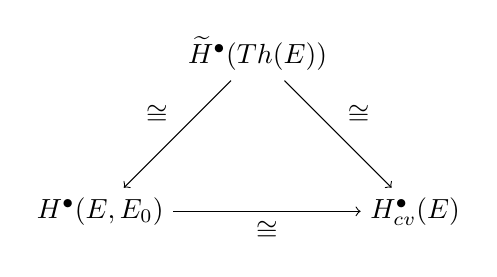
\begin{tikzpicture}[baseline=(current bounding box.east)]
                \node (TH) at (0, 0) {$\widetilde{H}^\bullet(\text{Th}(E))$};
                \node (R) at (-2, -2) {$H^\bullet(E, E_0)$};
                \node (CV) at (2, -2) {$H^\bullet_{cv}(E)$};
                \draw[->] (TH) -- node[above left]{$\cong$} (R);
                \draw[->] (TH) -- node[above right]{$\cong$} (CV);
                \draw[->] (R) -- node[below]{$\cong$} (CV);
            \end{tikzpicture}
        \end{gather}
    \end{property}

    \newdef{Thom spectrum}{\index{spectrum!Thom}
        Let $E\rightarrow M$ be a vector bundle. The Thom spectrum of $E$ is defined as the suspension spectrum of its Thom space. This can be written more explicitly as
        \begin{gather}
            (\Sigma^\infty\text{Th}(E))_n\cong\text{Th}(\mathbb{R}^n\oplus E)
        \end{gather}
        because of the existence of a homeomorphism $\text{Th}(\mathbb{R}^n\oplus E)\cong\Sigma^n\text{Th}(E)$.

        Let us now consider the sequence $\seq{\xi}$ of universal vector bundles. For every $\xi_n$ we define the $n^{th}$ component space as follows:
        \begin{gather}
            MO_n := \text{Th}(\xi_n).
        \end{gather}
        The Whitney sum $\xi_n\oplus\mathbb{R}$ can be obtained as a pullback of $\xi_{n+1}$. This map induces a map $\Sigma MO_n\rightarrow MO_{n+1}$, which gives the $n^{th}$ structure map of ''the'' Thom spectrum $MO$.\footnote{Note that the Thom spectrum as defined here is not an $\Omega$-spectrum \ref{topology:spectrum}, it is merely a sequential spectrum (prespectrum).}
    }

    \newdef{Euler class}{\index{Euler!class}
        Consider a vector bundle $E\rightarrow M$ together with its Thom class $\Phi$. The Euler class $e(E)$ is defined as the pullback $s_0^*\Phi$ of the Thom class along the zero section of $E$.
    }
    \begin{property}
        If the orientation of $E$ is reversed, the Euler class changes sign.
    \end{property}
    The following property distinguishes the Euler class among all characteristic classes of $E$:
    \begin{property}[Normalization]
        If the vector bundle admits a nowhere-vanishing section, its Euler class vanishes.
    \end{property}

\subsection{\v{C}ech-de Rham complex}\label{section:cech_de_rham}

    \begin{theorem}[Mayer-Vietoris sequence]\index{Mayer-Vietoris sequence}
        Consider a smooth manifold $M$ with an open covering $U\cup V$. The cohomology of $U,V$ is related to that of $M$ by the following short exact sequence:
        \begin{gather}
            0\longrightarrow H^\bullet(M)\longrightarrow H^\bullet(U)\oplus H^\bullet(V)\longrightarrow H^\bullet(U\cap V)\longrightarrow 0
        \end{gather}
        where the second arrow acts by restriction and the third one maps $(\omega,\rho)$ to $\rho-\omega$.
    \end{theorem}

    \newdef{\v{C}ech-de Rham complex}{
        Consider an open cover $\mathcal{U}=\{U_i\subseteq M\}_{i\in I}$ of a smooth manifold $M$.\footnote{Some authors require $I$ to be countable.} By $U_{i_0\ldots i_{k-1}}$ we denote the $k$-fold intersection $U_{i_0}\cap\cdots\cap U_{i_{k-1}}$. For all $k$ we define maps (where we suppress the label $k$) \[\delta_j:\Omega^\bullet(U_{i_0\ldots i_{k-1}})\rightarrow\prod_\alpha\Omega^\bullet(U_{i_0\ldots i_{j-1}\alpha i_j\ldots i_{k-1}})\] induced by the inclusions \[\iota_j:U_{i_0\ldots i_k}\hookrightarrow U_{i_0\ldots i_{j-1}i_{j+1}\ldots i_k}\] that ''ignore'' the $j^{th}$ open set. A total coboundary map $\delta$ is then defined as the alternating sum of the $\delta_i$'s:
        \begin{gather}
            (\delta\omega)_{i_0\ldots i_k} = \sum_{j=0}^k(-1)^i\omega_{i_0\ldots\widehat{i_j}\ldots i_k}
        \end{gather}
        for $\omega\in\prod\Omega^\bullet(U_{i_0\ldots i_{k-1}})$. It can be shown that $\delta$ is indeed a coboundary, i.e. $\delta^2=0$. The double complex $C^p(\mathcal{U}; \Omega^q):=\prod\Omega^q(U_{i_0\ldots i_p})$ with total differential $D=\delta+(-1)^pd$, where $d$ is the ordinary de Rham differential, is called the \v{C}ech-de Rham complex.
    }

    The Mayer-Vietoris sequence can be generalized to a statement for the \v{C}ech-de Rham complex:
    \begin{property}[Mayer-Vietoris sequence]
        The horizontal complex
        \begin{gather}
            0\longrightarrow\Omega^\bullet(M)\longrightarrow\prod_{i_0}\Omega^\bullet(U_{i_0})\longrightarrow\prod_{i_0,i_1}\Omega^\bullet(U_{i_0i_1})\longrightarrow\cdots
        \end{gather}
        is acyclic, i.e. the $\delta$-cohomology of the \v{C}ech-de Rham complex vanishes.
    \end{property}

    An important corollary is that one can compute the (de Rham) cohomology of $M$ using the above double complex:
    \begin{theorem}
        The restriction map $\Omega^\bullet(M)\rightarrow C^\bullet(\mathcal{U}; \Omega^\bullet)$ induces an isomorphism in cohomology.
    \end{theorem}
    One can also augment the \v{C}ech-de Rham complex in the other direction by the kernel of the de Rham differential in degree 1. These are the locally constant functions on the intersections $U_{i_0\ldots i_p}$. The cohomology of this augmenting sequence $C^\bullet(\mathcal{U}, \underline{\mathbb{R}})$ is called the \textbf{\v{C}ech cohomology} of $M$.\index{Cech!cohomology} By the same reason as for why the Mayer-Vietoris sequence implied the above theorem, we obtain the following theorem:
    \begin{theorem}[\v{C}ech $=$ de Rham]
        For a smooth manifold $M$, admitting a good cover $\mathcal{U}$, the \v{C}ech cohomology of $\mathcal{U}$ is isomorphic to the de Rham cohomology of $M$:
        \begin{gather}
            H^\bullet(M)\cong\check{H}^\bullet(\mathcal{U}; \underline{\mathbb{R}}).
        \end{gather}
    \end{theorem}
    \begin{result}
        All compact manifolds admit a finite good cover and hence have finite-dimensional de Rham cohomology.
    \end{result}

    We will now construct a generalization of \v{C}ech cohomology. The notation $\underline{\mathbb{R}}$ above should remind us of example \ref{sheaf:constant_sheaf}, i.e. $\underline{\mathbb{R}}$ denotes the sheaf of locally constant functions with values in $\mathbb{R}$. Similarly $\Omega^\bullet$ should be regarded as the sheaf of differential forms.
    \newdef{\v{C}ech cohomology}{\index{Cech!cohomology}
        Let $\mathcal{F}$ be a (pre)sheaf of Abelian groups. For an open cover $\mathcal{U}=\{U_i\subseteq M\}_{i\in I}$ we define the cochain groups
        \begin{gather}
            C^p(\mathcal{U};\mathcal{F}) := \prod_{i_0<\cdots<i_p}\mathcal{F}(U_{i_0\ldots i_p})
        \end{gather}
        for all $p\in\mathbb{N}$ as before. Since the (pre)sheaf takes values in Abelian groups we can define the subtraction of elements and hence the definition of the differential $\delta$ still makes sense:
        \begin{gather}
            \delta := \sum_{i=0}^k(-1)^i\mathcal{F}(\iota_i)
        \end{gather}
        where $\iota_i$ are the inclusion maps as before. The $\delta$-cohomology of the complex $C^\bullet(\mathcal{U}; \mathcal{F})$ is called the \v{C}ech cohomology of $\mathcal{U}$ with values in $\mathcal{F}$.

        By taking the direct limit over the direct system of open covers of a smooth manifold $M$ (the partial ordering is given by refinement of covers) one can define the \v{C}ech cohomology $\check{H}^\bullet(M; \mathcal{F})$ of $M$ with values in $\mathcal{F}$.
    }

    By noting that good covers are \textit{cofinal} in the set of open covers one can obtain the following theorem:
    \begin{theorem}[\v{C}ech $=$ de Rham, bis]
        For a smooth manifold the \v{C}ech cohomology of $M$ with values in $\underline{\mathbb{R}}$ is isomorphic to the de Rham cohomology of $M$:
        \begin{gather}
            H^\bullet(M)\cong\check{H}^\bullet(M;\underline{\mathbb{R}}).
        \end{gather}
    \end{theorem}

    \begin{example}[Zeroth cohomology]
        From the general definition of cohomology groups and the specific form of the coboundary operator we find that \[\omega_{\alpha_0}|_{U_{\alpha_0}\cap U_{\alpha_1}}=\omega_{\alpha_1}|_{U_{\alpha_0}\cap U_{\alpha_1}}\] for all $\alpha_0\neq\alpha_1$ and $\omega\in\check{H}^0(M;\mathcal{F})$. This is exactly the defining relation for the (global) sections of $\mathcal{F}$ and hence we obtain (as usual)
        \begin{gather}
            \check{H}^0(M;\mathcal{F})\cong\mathcal{F}(M).
        \end{gather}
    \end{example}

\subsection{Non-orientable manifolds}

    \newdef{Twisted cohomology}{\index{cohomology!twisted}
        Let $E\rightarrow M$ be a flat vector bundle over $M$. By construction \ref{diff:twisted_differential} we know that the algebra $\Omega^\bullet(M)\otimes E$ can be given the structure of a differential graded algebra \ref{linalgebra:dg_algebra} and hence gives rise to a cohomology theory $H^\bullet(M; E)$. This is called the $E$-twisted de Rham cohomology of $M$.
    }
    \begin{remark}
        By the remark following construction \ref{diff:twisted_differential} we should pay attention to what trivialization was used in the construction of $H^\bullet(M; E)$. It can be shown that two trivializations give rise to the same $E$-twisted cohomology if they admit a common refinement for which the induced sections differ by a locally constant matrix $a\in\text{GL}(n, \mathbb{R})$.
    \end{remark}

    If we take $E=o(M)$ to be the orientation line bundle over $M$, we obtain the (honest) densities of remark \ref{diff:honest_density}. The cohomology of this complex is simply called the \textbf{twisted de Rham cohomology}.
    \begin{property}[Isomorphisms]
        The twisted cohomologies defined by two trivializations induced from atlases on $M$ are isomorphic.\footnote{Although we almost always work with natural trivialization, i.e. where the open subsets of $M$ are obtained from charts on $M$, this is not technically necessary. For these ''exotic'' cases, the isomorphisms not always exist.}
    \end{property}
    \begin{property}[Trivial twisting]
        If $M$ is orientable, its twisted cohomology is isomorphic to its ordinary (de Rham) cohomology. More generally, the $E$-twisted de Rham cohomology is isomorphic to the ordinary de Rham cohomology whenever $E$ is trivial.
    \end{property}

    Poincar\'e duality \ref{diff:poincare_duality} can be translated almost verbatim to the twisted case:
    \begin{theorem}[Poincar\'e duality]\index{Poincar\'e!duality}
        Integration of densities induces the following isomorphism:
        \begin{gather}
            H^k(M)\cong\left(H^{m-k}_c(M; o(M))\right)^*.
        \end{gather}
        If $M$ is of finite type, the converse also holds:
        \begin{gather}
            H^k_c(M)\cong\left(H^{m-k}(M; o(M))\right)^*.
        \end{gather}
    \end{theorem}
    The Thom isomorphism also holds for non-orientable bundles:
    \begin{theorem}[Thom isomorphism]\index{Thom!isomorphism}
        Let $E\rightarrow M$ be a rank-$n$ vector bundle. Fibre integration gives the following isomorphism:
        \begin{gather}
            H^{\bullet+n}_{cv}(E)\cong H^\bullet(M; o(E)).
        \end{gather}
    \end{theorem}

\section{Differential operators}

    In this section we generalize the notion of PDEs and ellipticity (see section \ref{pde:section:higher_dimensions}) to vector bundles.

    \newdef{Differential operator}{\index{differential!operator}\index{elliptic!operator}
        A (linear) differential operators between two vector bundels $E, F$ over the same base manifold $X$ is a linear map $C^\infty(E)\rightarrow C^\infty(F)$ that can locally be expressed as a system of partial differential equations.

        The (principal) symbol of this operator is then defined as the (principal) symbol of the associated PDE. By extension we call the differential operator \textbf{elliptic} if its associated PDE is elliptic.
    }

\subsection{Elliptic complexes}

    \newdef{Elliptic complexes}{
        Consider a collection of vector bundles $\{\pi_i:E_i\rightarrow M\}_{i\in\mathbb{N}}$ together with a collection of differential operators $\{D_i:C^\infty(E_i)\rightarrow C^\infty(E_{i+1})\}_{i\in\mathbb{N}}$. We call this system an elliptic complex if it is a cochain complex, i.e. $D_{i+1}\circ D_i = 0$, and if the induced sequence $\{\sigma_p(\xi)(D_i)\}_{i\in\mathbb{N}}$ is exact for all $x\in M$ and $\xi\neq0$.
    }

    ?? COMPLETE ??

\section{Linear connections}\label{section:linear_connections}

    \newdef{Koszul connection}{\index{connection!Koszul}\label{manifolds:koszul_connection}
        Let $\pi: E\rightarrow M$ be a vector bundle over a smooth manifold $M$. A Koszul connection (or \textbf{linear connection)} on $E$ is a (smooth) linear map $\nabla:\Gamma(E)\rightarrow\Gamma(T^*M\otimes E)$ satisfying the Leibniz property
        \begin{gather}
            \nabla(f\sigma) = f\nabla\sigma + df\otimes\sigma
        \end{gather}
        for all $f\in C^\infty(M)$.
    }
    \begin{property}
        Because $\nabla\sigma$ takes a vector field as input, which is a $C^\infty(M)$-linear operation, we obtain
        \begin{gather}
            \nabla_{fX + Y}\sigma = f\nabla_X\sigma + \nabla_Y\sigma.
        \end{gather}
    \end{property}

    \begin{formula}
        Let $E, E'$ be two vector bundles over the same manifold $M$. Koszul connections on $E$ and $E'$ induce a connection on the tensor product bundle $E\otimes E'$ as follows:
        \begin{gather}
            \nabla(X\otimes Y) := \nabla X\otimes Y + X\otimes\nabla Y
        \end{gather}
        for $X\in\Gamma(E), Y\in\Gamma(E')$.
    \end{formula}

    \begin{example}[Affine connection]\index{connection!affine}
        Let $M$ be a smooth manifold. An affine connection $\nabla:\mathfrak{X}(M)\times\mathfrak{X}(M)\rightarrow \mathfrak{X}(M)$ is a Koszul connection on the tangent bundle.
    \end{example}

    \begin{property}[Local behaviour]
        Consider a vector $v\in T_pM$. If two vector fields $X, Y\in \Gamma(TM)$ are equal on some neighbourhood $U$ of $p$ then $\nabla_vX = \nabla_vY$ on $U$. Furthermore, given a curve $c:[0, 1]\rightarrow M$ and two vector fields $X, Y\in\Gamma(TM)$ such that $X\circ c = Y\circ c$ we find that $\nabla_{\dot c}X = \nabla_{\dot c}Y$. Hence we see that an affine connection only depends on the local behaviour of the given section.
    \end{property}
    \begin{remark}
        The above property shows the major difference between the Lie derivative and the covariant derivative when acting on sections of the tangent bundle $\sigma$. Lie derivatives depend on the local behaviour of both $X$ and $\sigma$. The covariant derivative on the other hand only depends on the value of $X$ at $p\in M$ and on the local behaviour of $\sigma$.
    \end{remark}

    \begin{property}[Affinity]
        Consider two affine connections $\nabla, \overline\nabla$ on a smooth manifold $M$. The operator $\nabla-\overline\nabla$ is an endormorphism of $E$, i.e. $\nabla-\overline\nabla\in\Omega^1(M;\text{End}(E))$. It follows that the set of affine connections forms an affine space (hence the name).
    \end{property}

    \newdef{Parallel tensor fields}{\index{parallel}
        A tensor field $T$ is said to be parallel with respect to a connection $\nabla$ if it satisfies $\nabla T = 0$.
    }
    \begin{example}
        Important examples in the case of the Levi-Civita connection on a Riemannian manifold are the volume form Vol and the metric $g$ (see chapter \ref{chapter:riemann}).
    \end{example}

    \newdef{Connection coefficients}{\index{Christoffel symbols}
        Let $E$ be a smooth rank-$k$ vector bundle. Consider a Koszul connection $\nabla$, a (local) frame $\{e_i\}_{1\leq i\leq k}$ and a (local) coframe $\{f^i\}_{1\leq i\leq k}$ of $E$. For every vector field $e_i$ one can (locally) write
        \begin{gather}
            \nabla e_i = \Gamma^k_{\ ji}e_k\otimes f^j.
        \end{gather}
        The quantities $\Gamma^k_{\ ji}$ are called the connection coefficients or \textbf{Christoffel symbols} of $\nabla$. For a general vector field $\sigma = \sigma^ie_i$ one then obtains (if $\{e_i,f^i\}_{1\leq i\leq k}$ are coordinate-induced):
        \begin{align}
            \nabla\sigma &= (\nabla\sigma^i)\otimes e_i + \sigma^i(\nabla e_i)\nonumber\\
            &= (\partial_j\sigma^k)e_k\otimes f^j + \sigma^i(\Gamma^k_{\ ji}e_k\otimes f^j)\nonumber\\
            &= (\partial_j\sigma^k + \Gamma^k_{\ ji}\sigma^i)e_k\otimes f^j.
        \end{align}
    }

\subsection{Induced connections}

    \begin{formula}[Connection on tensors]
        Applying the Leibniz property of a Koszul connection to tensor contractions gives us the following form of the induced connection on the $(s, k)$-tensor bundle:
        \begin{align}
            \nabla_YT(\omega^1,\ldots, \omega^s, X_1,\ldots, X_k) := Y\Big(&T(\omega^1,\ldots, \omega^s, X_1,\ldots, X_k)\Big)\nonumber\\
            &- \sum_{i=1}^sT(\omega^1,\ldots, \nabla_Y\omega^i,\ldots, \omega^s, X_1,\ldots, X_k)\nonumber\\
            &- \sum_{i=1}^kT(\omega^1,\ldots, \omega^s, X_1,\ldots, \nabla_YX_i,\ldots, X_k)
        \end{align}
        where $Y, X_1,\ldots, X_k\in\mathfrak{X}(M)$ and $\omega^1,\ldots,\omega^s\in\Omega^1(M)$.
    \end{formula}

    \begin{result}
        By noting that the covariant derivative of a vector field is a vector-valued differential form, we can use the previous formula to compute the covariant derivative of the covariant derivative:
        \begin{gather}
            (\nabla_X\nabla)_YZ = \nabla_X(\nabla_YZ) - \nabla_{\nabla_XY}Z - \nabla_Y(\nabla_XZ).
        \end{gather}
        We added parentheses to make it clear that the outer covariant derivatives act on the result of the inner derivatives. If we would not have added these parentheses, we could have confused these terms with the second covariant derivative (whose definition also follows from a Leibniz-type argument):
        \begin{gather}
            \nabla^2_{X, Y}S : = \nabla_X(\nabla_YS) - \nabla_{\nabla_XY}S.
        \end{gather}
    \end{result}

    As an example of the second covariant derivative we give the definition of the Hessian on arbitrary smooth manifolds:
    \newdef{Hessian}{\index{Hessian}
        Consider a smooth manifold with connection $\nabla$. The Hessian of a function $f\in C^\infty(M)$ is defined as the iterated covariant derivative:
        \begin{gather}
            \text{Hess}(f) := \nabla^2f
        \end{gather}
        where one should note that by the above definition the first covariant derivative also acts on the second one, i.e\mnote{\dbend}
        \begin{gather}
            \nabla\nabla f(X, Y) = \nabla_X(\nabla_Yf) - \nabla_{\nabla_XY}f.
        \end{gather}
        For a scalar function we know that $\nabla f = df$ and for covector fields we know that (in local coordinates) \[\nabla_i\sigma_j = \partial_i\sigma_j - \Gamma^k_{ij}\sigma_k\] where $\Gamma^k_{ij}$ are the connection coefficients. Combining these facts we obtain the following local formula for the Hessian of $f$:
        \begin{gather}
            \text{Hess}(f) = \left(\frac{\partial^2f}{\partial x_i\partial x_j} - \Gamma^k_{ij}\pderiv{f}{x_k}\right)dx^i\otimes dx^j.
        \end{gather}
    }

    \newdef{Pullback connection}{\index{connection!pullback}
        Let $E\rightarrow M$ be a vector bundle with Koszul connection $\nabla$ and let $f:M'\rightarrow M$ be a smooth map. On the pullback bundle\footnote{See definition \ref{manifolds:pullback_bundle}.} $f^*E$ there exists a unique Koszul connection $\nabla'$ satisfying
        \begin{gather}
            \nabla'(f^*\chi) = f^*(\nabla\chi)
        \end{gather}
        for any section of $E$.
    }
    \newdef{Invariant connection}{\index{connection!invariant}
        Let $G$ be a Lie group acting on a vector bundle $E\rightarrow M$. A Koszul connection $\nabla$ on $E$ is said to be invariant with respect to the $G$-action if it satisfies:
        \begin{gather}
            g^*\nabla = \nabla
        \end{gather}
        for all $g\in G$.
    }
% \chapter{Principal Bundles}\label{chapter:principal_bundles}

    The main reference for this chapter is~\citet{sontz_principal_2015}. Ths chapter uses the language of (Lie) group theory quite heavily. For all things related to group theory, the reader is referred to \cref{section:groups} and \cref{section:group_actions}. For more information on Lie groups and their associated Lie algebras, the reader is referred to \cref{chapter:lie}.

    \minitoc

\section{Principal bundles}

    \newdef{Principal bundle}{\index{principal!bundle}
        A fibre bundle $\pi:P\rightarrow B$ equipped with a right action $\rho:P\times G\rightarrow B$ that satisfies two properties:
        \begin{enumerate}
            \item\textbf{Free action}: $\rho$ is free. This implies that the orbits are isomorphic to the structure group.
            \item\textbf{Fibrewise transitivity}: The action preserves fibres, i.e.~$y\cdot g\in F_b$ for all $y\in F_b,g\in G$. In turn this implies that the fibres over $B$ are exactly the orbits of $\rho$.
        \end{enumerate}
        Together these properties imply that the typical fibre $F$ and structure group $G$ can be identified. The right action of $G$ on $P$ will often be denoted by $R_g$ (unless this would give conflicts with the same notation for the action of $G$ on itself).
    }
    \begin{remark}[$G$-torsor]\label{bundle:fibre_torsor}
        Although the fibres are homeomorphic to $G$, they do not carry a group structure due to the lack of a distinct identity element. This turns them into $G$-torsors (\cref{group:torsor}). However, it is possible to locally endow the fibres with a group structure by choosing an element of every fibre to be the identity element.
    \end{remark}

    \begin{property}
        A corollary of the definition is that the bundle $\pi:P\rightarrow B$ is isomorphic to the bundle $\xi:P\rightarrow P/G$, where $P/G$ denotes the orbit space of $P$ with respect to the $G$-action (which can be proven to be proper) and $\xi$ is the quotient projection.
    \end{property}

    In fact this property can be used to give an alternative characterization of smooth principal bundles.
    \begin{property}[Quotient manifold theorem]\label{bundle:quotient_manifold_theorem}
        Consider a smooth manifold $P$ equipped with a free and proper (right) action of a Lie group $G$. The following statements hold:
        \begin{itemize}
            \item The orbit space $P/G$ is a smooth manifold.
            \item The projection $P\rightarrow P/G$ is a submersion.
            \item $P$ is principal $G$-bundle over $P/G$.
        \end{itemize}
    \end{property}

    \begin{property}[Dimension]\label{bundle:principal_bundle_dimension}
        The dimension of $P$ is given by
        \begin{gather}
            \dim(P) = \dim(B) + \dim(G)\,.
        \end{gather}
    \end{property}

    \begin{property}
        Every local trivialization $\varphi_i$ is $G$-equivariant:
        \begin{gather}
            \varphi_i(z\cdot g) = \varphi_i(z)\cdot g\,.
        \end{gather}
    \end{property}

    \newdef{Principal bundle map}{\index{bundle!map}
        A bundle map between principal $G$-bundles is a pair of morphisms $(f_B,f_P)$ such that:
        \begin{enumerate}
            \item $(f_B,f_P)$ is an ordinary bundle map (\cref{bundle:bundle_map}).
            \item $f_P$ is $G$-equivariant.
        \end{enumerate}
    }

    The following property proves that the equivariance condition on principal bundle maps is, in fact, a very strong condition.
    \begin{property}
        Every principal bundle map covering the identity is an isomorphism.
    \end{property}

    \newdef{Vertical automorphism}{\index{vertical!automorphism}\index{gauge!transformation}\label{bundle:vertical_automorphism}
        Consider a principal $G$-bundle $\pi:P\rightarrow B$. An automorphism $f$ of this bundle is said to be vertical if it covers the identity, i.e.~$\pi\circ f=\pi$. It is the subgroup $\Aut_V(P)\subset\Aut(P)$ of vertical automorphisms that is known as the \textbf{group of gauge transformations} or \textbf{gauge group}\footnote{This should not be confused with the structure group $G$, which is also sometimes called the gauge group in physics.} in physics.
    }
    \sremark{It should be clear that the above definition can easily be generalized to arbitrary fibre bundles.}

\subsection{Associated bundles}

    \begin{construct}[Associated principal bundle]\label{bundle:associated_bundle_construction}
        For every fibre bundle one can construct an associated principal $G$-bundle by replacing the fibre $F$ by $G$ itself using the fibre bundle construction theorem \ref{bundle:fibre_bundle_construction_theorem}, where the left action of $G$ is given by left multiplication in $G$.
    \end{construct}

    \begin{property}[Triviality]
        A fibre bundle $\xi$ is trivial if and only if its associated principal bundle is trivial. More generally, two fibre bundles are isomorphic if and only if their associated principal bundles are isomorphic.
    \end{property}

    \begin{example}[Frame bundle]\index{frame!bundle}\label{bundle:frame_bundle}
        Let $V$ be an $n$-dimensional vector space and denote the set of frames (\cref{linalgebra:frame}) of $V$ by $FV$. It follows from the fact that every basis transformation is given by the action of an element of the general linear group that $FV$ is isomorphic to $\GL(V)\cong\GL(\mathbb{R}^n)$.

        Given a rank-$n$ vector bundle $E$, one can construct an associated principal bundle by replacing every fibre $\pi^{-1}(b)$ by $F\bigl(\pi^{-1}(b)\bigr)\cong\GL(\mathbb{R}^n)$. The right action on this bundle by $g\in\GL(\mathbb{R}^n)$ is given by the basis transformation $\widetilde{e}_j=g^i_je_i$. This bundle, the frame bundle, is denoted by $FE$ or $FM$ in the case of the tangent bundle $E=TM$.
    \end{example}

    \begin{construct}[Associated bundle to a principal bundle]\index{associated!bundle}\label{bundle:associated_bundle}
        Consider a principal $G$-bundle $\pi:P\rightarrow B$ and let $F$ be a space equipped with a left $G$-action $\vartriangleright$. One can construct an associated bundle $P_F\equiv P \times_\vartriangleright F$ in the following way:
        \begin{enumerate}
            \item Define an equivalence relation $\sim_G$ on the product space $P\times F$ by
                \begin{gather}
                    \label{bundle:associated_bundle_equivalence}
                    (p,f)\sim_G(p',f')\iff\exists g\in G:(p',f') = (p\cdot g,g^{-1}\vartriangleright f)\,.
                \end{gather}
            \item Define the total space of the associated bundle as the following quotient space:
                \begin{gather}
                    P_F := (P\times F)/\sim_G\,.
                \end{gather}
            \item Define the projection $\pi_F:P_F\rightarrow B$ as follows:
                \begin{gather}
                    \pi_F:[p,f]\mapsto\pi(p)\,,
                \end{gather}
            where $[p,f]$ is the equivalence class of $(p,f)\in P\times F$ in $P_F$.
        \end{enumerate}
    \end{construct}
    \begin{example}[Tangent bundle]
        Starting from the frame bundle $FM$ over a manifold $M$, one can reconstruct, up to a bundle isomorphism, the tangent bundle $TM$ in the following way. Consider the left $G$-action $\vartriangleright$ of a matrix group given by
        \begin{gather}
            \vartriangleright:G\times\mathbb{R}^n\rightarrow\mathbb{R}^n:(g\vartriangleright f)^i \mapsto g^i_{\ j}f^j\,.
        \end{gather}
        The tangent bundle is isomorphic to the associated bundle $FM\times_\vartriangleright\mathbb{R}^n$, where the bundle map is defined as $[e,v]\mapsto v^ie_i\in TM$.
    \end{example}

    \begin{example}[Adjoint bundle]\index{adjoint!bundle}
        Consider a principal $G$-bundle $P$. $G$ acts on itself by conjugation through the adjoint action
        \begin{gather}
            \mathrm{Ad}:G\times G\rightarrow G:(g,h)\mapsto g^{-1}hg\,.
        \end{gather}
        This action induces an associated bundle $\mathrm{Ad}(P):=P\times_GG$, suitable named the adjoint bundle of $P$.
    \end{example}
    \begin{property}[Vertical automorphisms]
        There exists an isomorphism between the vertical automorphism group $\Aut_V(P)$ and the group of sections of the adjoint bundle $\mathrm{Ad}(P)$.
    \end{property}

    \begin{construct}[Associated bundle map]\index{bundle!map}
        Given a principal bundle map $(f_B,f_P)$ between two principal bundles one can construct an associated bundle map between any two of their associated bundles with the same typical fibre in the following way:
        \begin{itemize}
            \item The total space map $\widetilde{f}_P:P\times_GF\rightarrow P'\times_{G'}F$ is given by
                \begin{gather}
                    \widetilde{f}_P([p,f]) := [f_P(p),f]\,.
                \end{gather}
            \item The base space map is simply given by $f_B$ itself:
                \begin{gather}
                    \widetilde{f}_B(b) = f_B(b)\,.
                \end{gather}
        \end{itemize}
    \end{construct}

\subsection{Sections}

    Although every vector bundle has at least one global section, the zero section, a general principal bundle does not necessarily have a global section. This is made clear by the following property.
    \begin{property}[Trivial bundles]
        A principal $G$-bundle $P$ is trivial if and only if there exists a global section of $P$. Furthermore, there exists a bijection between the set of global sections $\Gamma(P)$ and the set of trivializations $\mathrm{Triv}(P)$.
    \end{property}
    \begin{result}\label{bundle:prin_section_triv}
        Every local section $\sigma:U\rightarrow P$ induces a local trivialization $\varphi$ by
        \begin{gather}
            \varphi^{-1}:(m,g)\mapsto\sigma(m)\cdot g\,.
        \end{gather}
        The converse is also true. Consider a local trivialization $\psi^{-1}:U\times G\rightarrow\pi^{-1}(U)$. A local section can be obtained by taking $\sigma(u):=\psi^{-1}(u,e)$.
    \end{result}

    \Cref{bundle:trivial_vector_bundle} can now be reformulated as follows.
    \begin{property}[Trivial vector bundles]
        A vector bundle is trivial if and only if its associated frame bundle admits a global section. This can easily be interpreted as follows. If one can for every fibre choose a basis in a smooth way, one can also express the restriction of any vector field to a fibre in terms of this basis in a smooth way.
    \end{property}

    \begin{property}[Higgs fields]\index{Higgs!field}\label{bundle:section_bijection}
        Let $\pbundle$ be a principal $G$-bundle and let $P_F$ be an associated bundle. There exists a bijection between the sections of $P_F$ and the $G$-equivariant maps $\phi:P\rightarrow F$, i.e.~maps satisfying $\phi(p\cdot g)=g^{-1}\cdot\phi(p)$.

        An explicit correspondence is given by
        \begin{gather}
            \sigma_\phi:M\rightarrow P_F:m\mapsto[p,\phi(p)]\,,
        \end{gather}
        where $p$ is any point in $\pi^{-1}(\{m\})$. This is well-defined due to \cref{bundle:associated_bundle_equivalence}. In the other direction, one finds
        \begin{gather}
            \label{bundle:section_bijection_phi}
            \phi_\sigma:P\rightarrow F:p\mapsto j_p^{-1}\circ\sigma(\pi(p))\,,
        \end{gather}
        where $j_p:F\rightarrow P_F:f\mapsto[p,f]$. Either of these maps is sometimes called a \textbf{Higgs field} in the physics literature.
    \end{property}

\section{Universal bundle}

    \newdef{Universal bundle}{\index{universal!bundle}\index{classifying!space}\label{bundle:classifying_space}
        Consider a topological group $G$. A universal bundle of $G$ is any principal bundle of the form \[G\hookrightarrow EG\rightarrow BG\] such that $EG$ is weakly contractible. The space $BG$ is called the \textbf{classifying space} of $G$.
    }
    \newdef{$n$-universal bundle}{
        A principal bundle with an $(n-1)$-connected total space.
    }
    \begin{property}[Delooping]\index{delooping}\label{bundle:delooping}
        For every topological group $G$, one can prove that the loop space of $BG$ is (weakly) homotopy equivalent to $G$ itself, i.e.~$\Omega BG\cong G$. As such, it also deserves the name of delooping.
    \end{property}
    \begin{property}[Groups]
        Let $G$ be a group regarded as a discrete topological space. Because the fundamental group of a topological group is Abelian by \cref{topology:abelian_fundamental_group}, the classifying space $BG$ is a group if and only if $G$ is Abelian.

        This also has an abstract nonsense generalization. The classifying space functor $\func{B}{TopGrp}{Top}$ is product-preserving and, hence, it maps group objects to group objects. So, Abelian groups are mapped to topological groups and, even better, to Abelian groups. An important consequence is that all Abelian topological groups are in particular infinite loop spaces.
    \end{property}

    \begin{property}[Classification]\label{bundle:classification}
        The collection of principal $G$-bundles over a paracompact Hausdorff space $X$ is in bijection with $[X,BG]$, the set of homotopy classes of continuous functions $f:X\rightarrow BG$. This bijection is given by the pullback-construction $f\mapsto f^*EG$.

        Due to the homotopical nature of this classification one can also replace $G$ by any homotopy equivalent space. For Lie groups the natural choice is a \textit{maximal compact subgroup} since these are deformation retracts and, hence, homotopy equivalent.
    \end{property}
    \begin{result}[Vector bundles]\index{vector!bundle}
        Since every vector bundle is uniquely related to its frame bundle, there exists a bijection between principal $\GL$-bundles and vector bundles. This implies that rank-$k$ vector bundles are classified by the homotopy mapping space $[X,B\!\GL(k)]$. Because $\mathrm{O}(k)$ is the maximal compact subgroup of $\GL(k)$, one also obtains the result that any real vector bundle over a paracompact space admits a \textit{Riemannian structure} (see \cref{chapter:riemann}).

        \Cref{bundle:vector_bundles_over_sphere} now follows from Eckmann--Hilton duality (\cref{topology:eckmann_hilton}) together with the above delooping property.
    \end{result}
    \begin{remark}
        There also exists a slightly different notion of universal bundles and their associated classifying property. When one requires the total space of the universal bundle to be contractible instead of weakly contractible, the mapping space only classifies numerable principal bundles (\cref{bundle:numerable_bundle}), but now over arbitrary bases.
    \end{remark}

    An explicit construction of the numerable universal bundle for any topological group $G$ was given by \indexauthor{Milnor}.
    \begin{construct}[\difficult{Milnor}]\index{Milnor!construction}
        First, consider the infinite join $E_\infty$ equipped with the strong topology. This space is constructed as the direct limit of finite joins (\cref{topology:join}): \[E_n=\underbrace{G\circ\cdots\circ G}_{n\text{ times}}\,,\] where $E_n$ is embedded in $E_{n+1}$ using the identity element, i.e.~every element of $E_\infty$ corresponds to an element of some finite join. Then, construct the quotient of $E_n$ (resp.~$E_\infty$) by the canonical right action of $G$ on $E_n$ (resp.~$E_\infty$). The bundle $p_n:E_n\rightarrow B_n$ (resp.~$p:E_\infty\rightarrow B_\infty$) is an $n$-universal bundle (resp.~$\infty$-universal bundle). It follows from the above property that $p:E_\infty\rightarrow B_\infty$ is a universal bundle for $G$.
    \end{construct}

    \begin{construct}[\difficult{Abstract nonsense}]
        Let $G$ be a topological group and consider the delooping (groupoid) $\mathbf{B}G$ from \cref{cat:group_delooping}. This groupoid can also be obtained as the action groupoid (\cref{cat:action_groupoid}) associated to the trivial action of $G$ on $\{\ast\}$. The regular action of $G$ on itself also induces an action groupoid $\mathbf{E}G:=G/\!/G$. The map $G\rightarrow\{\ast\}$ in turn induces a map of groupoids $\mathbf{E}G\rightarrow\mathbf{B}G$, which, under geometric realization as in \cref{model:classifying_space}, gives a universal bundle map.
    \end{construct}

\section{Connections}\label{section:connections}
\subsection{Vertical vectors}

    Because smooth fibre bundles are also smooth manifolds, one can define traditional concepts such as the tangent bundle. Due to the composite nature of these geometric objects, one can decompose the tangent bundle in horizontal and vertical (sub)bundles.
    \newdef{Vertical vector}{\index{vertical!bundle}
        Let $\bundle$ be a smooth fibre bundle. The subbundle
        \begin{gather}
            VE:=\ker(\pi_\ast)
        \end{gather}
        of $TE$ is called the \textbf{vertical (sub)bundle} over $E$. The sections of this bundle are called vertical vector fields.
    }
    For principal $G$-bundles an alternative definition exists.
    \begin{adefinition}
        Consider a smooth principal $G$-bundle $\pbundle$. First, construct a map $\iota_p$ for every element $p\in P$:
        \begin{gather}
            \iota_p:G\rightarrow P:g\mapsto p\cdot g\,.
        \end{gather}
        Then, define a tangent vector $v\in T_pP$ to be vertical if it lies in the image of $\iota_{p,\ast}$:
        \begin{gather}
            V_pP := \im(\iota_{p,\ast})\,.
        \end{gather}
        This definition is equivalent to the previous one because of the following short exact sequence:
        \begin{gather}
            \label{bundle:principal_bundle_exact_sequence}
            0\longrightarrow\mathfrak{g}\overset{\iota_{p,\ast}}{\longrightarrow}T_pP\overset{\pi_\ast}{\longrightarrow}T_pM\longrightarrow0\,.
        \end{gather}
    \end{adefinition}

    \begin{property}[Dimension]\label{bundle:vertical_dimension}
        It follows from the second definition that the vertical vectors of a principal $G$-bundle are nothing but the pushforward of the Lie algebra $\mathfrak{g}$ under the right action of $G$ on $P$. Furthermore, the exactness of the sequence implies that $\iota_{p,\ast}:\mathfrak{g}\rightarrow V_pP$ is an isomorphism of vector spaces. In particular, it implies that
        \begin{gather}
            \dim(V_pP) = \dim(\mathfrak{g}) = \dim(G)\,.
        \end{gather}
    \end{property}

    \newdef{Fundamental vector field}{\index{vector field!fundamental}\label{bundle:fundamental_vector_field}
        Let $P$ be a principal $G$-bundle and consider $A\in\mathfrak{g}$, where $\mathfrak{g}$ is the Lie algebra corresponding to $G$. The vertical vector field $A^\#:P\rightarrow TP$, given by
        \begin{gather}
            A^\#(p) := \iota_{p,\ast}A\in VpP\,,
        \end{gather}
        is called the fundamental vector field associated to $A$. Its action on any $f\in C^\infty(P)$ is given by
        \begin{gather}
            A^\#_p(f) = \left.\deriv{}{t}f\bigl(p\cdot\exp(tA)\bigr)\right|_{t=0}\,.
        \end{gather}
    }

    \begin{property}
        The construction of fundamental vector fields gives a Lie algebra morphism $\mathfrak{g}\rightarrow\mathfrak{X}(P)$:
        \begin{gather}
            [A,B]^\# = [A^\#,B^\#]\,,
        \end{gather}
        where the Lie bracket on the left is the one in $\mathfrak{g}$ and the Lie bracket on the right is the one in $\mathfrak{X}(P)$ given by \cref{bundle:lie_bracket}.
    \end{property}

    \begin{property}\label{bundle:vert_g_equivariance}
        The vertical bundle satisfies the following equivariance condition:
        \begin{gather}
            R_{g,\ast}(VpP) = V_{p\cdot g}P\,.
        \end{gather}
        By differentiating the equality
        \begin{gather}
            R_g\circ\iota_p = \iota_{p\cdot g}\circ\mathrm{ad}_{g^{-1}}
        \end{gather}
        and using \cref{lie:adjoint_representation} and \cref{bundle:fundamental_vector_field}, one can obtain the following algebraic reformulation:
        \begin{gather}
            R_{g,\ast}\bigl(A^\#(p)\bigr) = \bigl(\mathrm{Ad}_{g^{-1}}A\bigr)^\#(p\cdot g)\,.
        \end{gather}
    \end{property}

\subsection{Ehresmann connections}

    The definition of vertical vector fields was quite natural. The next step would be to define the horizontal subspace as a complementary subspace to $VP$. However, the exact sequence~\eqref{bundle:principal_bundle_exact_sequence} does not even split canonically, so one should make a choice of splitting.
    \newdef{Ehresmann connection}{\index{connection!Ehresmann}\index{horizontal!vector}\label{bundle:connection}
        Consider a smooth fibre bundle $E$. An (Ehresmann) connection on $E$ is the selection of a subspace $H_eE\leq T_eE$ for every $e\in E$ such that:
        \begin{enumerate}
            \item The horizontal and vertical bundles are complementary: $V_eE\oplus H_eE=T_eE$.
            \item The choice of subspace depends smoothly on $e\in E$ in the distributional sense (\cref{bundle:distribution}).
        \end{enumerate}
        The vectors in $H_eE$ are said to be \textbf{horizontal} (with respect to the chosen connection).
    }
    \newdef{Horizontal bundle}{\index{horizontal}
        The horizontal (sub)bundle $HE$ is defined as $\bigsqcup_{e\in E}H_eE$ with the bundle structure induced from $TE$.
    }

    \newdef{Principal connection}{\index{connection!principal}\label{bundle:principal_connection}
        A principal connection on a smooth principal $G$-bundle $P$ is a $G$-equivariant Ehresmann connection, i.e.~an Ehresmann connection for which the horizontal subspaces satisfy the following $G$-equivariance condition:
        \begin{gather}
            R_{g,\ast}(H_pP) = H_{p\cdot g}P\,.
        \end{gather}
    }
    \begin{remark*}
        Note that this condition was automatically satisfied for vertical bundles by \cref{bundle:vert_g_equivariance}.
    \end{remark*}

    \begin{property}[Dimension]\label{bundle:connection_dimensions}
        \nameCrefs{bundle:vertical_dimension}~\ref{bundle:principal_bundle_dimension} and~\ref{bundle:vertical_dimension}, together with the direct sum decomposition of $TP$, imply the following relation for all $p\in P$:
        \begin{gather}
            \dim(H_pP) = \dim(M)\,.
        \end{gather}
        All dimensional relations between the data of a principal bundle are now summarized:
        \begin{align}
            \dim(P) &= \dim(M) + \dim(G)\nonumber\\
            \dim(M) &= \dim(H_pP)\\
            \dim(G) &= \dim(V_pP)\nonumber
        \end{align}
        for all $p\in P$.
    \end{property}

    \newdef{Dual connection}{\index{dual!connection}
        First, define the dual of the horizontal bundle:
        \begin{gather}
            H_p^*P := \bigl\{h\in T_p^*P\bigm\vert\forall v\in V_pP:h(v)=0\bigr\}\,.
        \end{gather}
        It is the space of one-forms that vanish on the vertical subspace. A dual connection can then be defined as the selection of a vertical covector bundle $V_p^*P$ satisfying the conditions of \namecrefs{bundle:connection}~\ref{bundle:connection} and~\ref{bundle:principal_connection}, where $V$ and $H$ are to be interchanged. Note that, here, the horizontal subbundle is canonically defined while the vertical subbundle depends on a choice of complement.
    }
    This definition implies the following ones.
    \newdef{Horizontal and vertical forms}{\index{horizontal!form}\index{vertical!form}\label{bundle:horizontal_form}
        Let $\theta\in\Omega^k(P)$ be a differential $k$-form.
        \begin{itemize}
            \item $\theta$ is said to be horizontal if
            \begin{gather}
                \theta_p(v_1,\ldots,v_k) = 0
            \end{gather}
            whenever at least one of the $v_i$ is in $V_pP$.
            \item $\theta$ is said to be vertical if
            \begin{gather}
                \theta_p(v_1,\ldots,v_k) = 0
            \end{gather}
            whenever all of the $v_i$ are in $H_pP$.
        \end{itemize}
        For functions $f\in C^\infty(P)$ it is vacuously true that they are both vertical and horizontal.
    }
    \newdef{Tensorial form}{\index{tensorial}\index{basic}\label{bundle:tensorial_form}
        Consider a vector space $V$ equipped with a representation $\rho:G\rightarrow V$. A $V$-valued differential form $\theta\in\Omega^\bullet(P;V)$ on a principal $G$-bundle $\pbundle$ is said to be tensorial or \textbf{basic of type} $(V,\rho)$ if it is horizontal and if it satisfies the equivariance condition
        \begin{gather}
            R_g^*\theta = \rho(g^{-1})\circ\theta\,.
        \end{gather}
        Forms satisfying this definition admit an important reinterpretation. Let $E:=P\times_\rho V$ be the associated vector bundle of $(V,\rho)$. Tensorial $k$-forms of type $(V,\rho)$ are naturally isomorphic to $E$-valued $k$-forms on $M$. The isomorphism is given fibrewise by
        \begin{gather}
            \label{bundle:tensorial_form_equivalence}
            \tau|_u:\Omega^\bullet|_{\pi(u)}(M;P\times_\rho V)\rightarrow\Omega^\bullet|_u(P;V):\phi\mapsto f^{-1}_u(\pi^*\phi)\,,
        \end{gather}
        where $f_u:V\rightarrow E_{\pi(u)}\cong(\pi^*E)_u:v\mapsto[u,v]$. This is a generalization of correspondence~\ref{bundle:section_bijection}.
    }

\subsection{Connection forms}

    \newdef{Connection one-form}{\index{connection!form}
        Let $P$ be a principal bundle $G$-bundle. A connection one-form, associated to a given principal connection, is a $\mathfrak{g}$-valued one-form $\omega\in\Omega^1(P;\mathfrak{g})$ that satisfies the following two conditions:
        \begin{enumerate}
            \item\textbf{Cancellation}:
            \begin{gather}
                \omega(A^\#) = A
            \end{gather}
            for all $A\in\mathfrak{g}$.
            \item\textbf{Equivariance}:
            \begin{gather}
                \omega\circ R_{g,\ast} = \mathrm{Ad}_{g^{-1}}\circ\omega
            \end{gather}
            for all $g\in G$.
        \end{enumerate}
        The horizontal subspaces are recovered as the kernel of the connection one-form:
        \begin{gather}
            H_pP = \ker(\omega|_p)\,.
        \end{gather}
    }
    \begin{formula}
        Given a principal connection on a principal $G$-bundle $P$, the associated connection one-form is given by the following map:
        \begin{gather}
            \omega := (\iota_{p,\ast})^{-1}\circ\pr_{\text{Vert}}\,,
        \end{gather}
        where $\pr_{\text{Vert}}$ is the projection $TP\rightarrow VP$.
    \end{formula}

    \begin{property}[Pullback connection]\index{connection!pullback}
        Consider two principal $G$-bundles $P_1,P_2$. Let $\omega$ be a connection one-form on $P_1$ and let $F:P_1\rightarrow P_2$ be a bundle map. The pullback $F^*\omega$ gives a principal connection on $P_2$.
    \end{property}

    \newdef{Maurer--Cartan form}{\index{Maurer--Cartan!form}\index{Cartan!(connection) form|see{Maurer--Cartan}}
        For every $g\in G$, the tangent space $T_gG$ is isomorphic to $T_eG\equiv\mathfrak{g}$. A canonical isomorphism $T_gG\rightarrow\mathfrak{g}$ is given by the Maurer--Cartan form
        \begin{gather}
            \Omega|_g := L_{g^{-1},\ast}\,.
        \end{gather}
    }
    \begin{construct}
        Consider the one-point manifold $M=\{\ast\}$. When constructing a principal $G$-bundle over $M$, one can see that the total space $P=\{\ast\}\times G$ can be identified with the structure group $G$. From the relations in \cref{bundle:connection_dimensions}, it follows that the horizontal spaces are null-spaces, which trivially defines a smooth distribution and a connection in the sense of Ehresmann (\cref{bundle:connection}), and that the vertical spaces are equal to the tangent spaces, i.e.~$V_gG=T_gG$, where the identification $P\cong G$ (as manifolds) is used.

        The simplest way to define a connection form on this bundle would be the trivial projection $\mathbbm{1}_{TP}:TP\rightarrow TP=VP$. However, the image of this map would be $T_gG$ and not $\mathfrak{g}$ as required. This can be solved by using the Maurer--Cartan form:
        \begin{gather}
            \omega = \Omega\,.
        \end{gather}
    \end{construct}
    \begin{property}[Uniqueness]
        The Maurer--Cartan form is the unique principal connection on the bundle $G\hookrightarrow G\rightarrow\{\ast\}$.
    \end{property}

    \newdef{Darboux derivative}{\index{Darboux!derivative}\index{integral}\index{primitive}
        Consider a smooth function $f:M\rightarrow G$ between a manifold and a Lie group. The Darboux derivative of $f$ is defined as follows:
        \begin{gather}
            \omega_f := f^*\Omega\,.
        \end{gather}
        The function $f$ is called an \textbf{integral} or \textbf{primitive} of $\omega_f$.
    }

    \begin{property}
        Let $M$ be a connected manifold. If two functions $f,\widetilde{f}:M\rightarrow G$ have the same Darboux derivative, there exists an element $g\in G$ such that $f(p)=g\cdot\widetilde{f}(p)$ for all $p\in M$.
    \end{property}
    \begin{example}[Real line]
        In the case of $M=G=\mathbb{R}$, one recovers the ordinary behaviour of derivatives. When two functions $f,\widetilde{f}:\mathbb{R}\rightarrow\mathbb{R}$ have the same derivative, they are equal up to an additive constant.
    \end{example}

    \begin{theorem}[Fundamental theorem of calculus]\index{fundamental theorem!of calculus}\index{Maurer--Cartan!equation}\label{bundle:mc_equation}
        Consider a smooth manifold $M$ and a Lie group $G$ with Lie algebra $\mathfrak{g}$. If $\omega:TM\rightarrow\mathfrak{g}$ satisfies the Maurer--Cartan equation
        \begin{gather}
            \dr\omega + \frac{1}{2}[\omega\wedge\omega] = 0\,,
        \end{gather}
        there exists (locally) a smooth function $f:M\rightarrow G$ such that $\omega=f^*\Omega$.
    \end{theorem}

\subsection{Local representations}

    \newdef{Yang--Mills field}{\index{Yang--Mills!field}\label{bundle:yang_mills_field}
        Consider a principal $G$-bundle $\pbundle$ and an open subset $U\subseteq M$. Given a principal connection $\omega$ on $P$ and a local section $\sigma:U\rightarrow P$, the Yang--Mills field $\omega^U\in\Omega^1(U; \mathfrak{g})$ is defined as follows:
        \begin{gather}
            \omega^U := \sigma^*\omega\,.
        \end{gather}
    }
    \newdef{Local representation}{
        Consider a principal bundle $P$ and let $(U,\varphi)$ be a bundle chart on $P$. The local representation of a principal connection $\omega$ on $P$ with respect to the chart $(U,\varphi)$ is defined as $(\varphi^{-1})^*\omega$.
    }

    \begin{formula}
        Consider a principal connection $\omega$ on a principal $G$-bundle $\pbundle$. Because of \cref{bundle:prin_section_triv}, every local section $\sigma:U\rightarrow P$ induces both a Yang--Mills field $\omega^U$ and a local representation of $\omega$. These two forms are related by the following equation:
        \begin{gather}
            \omega|_{(m,g)}(v,A) = \mathrm{Ad}_{g^{-1}}\bigl(\omega^U_m(v)\bigr) + \Omega_g(A)\,,
        \end{gather}
        where $v\in T_mU$ and $A\in\mathfrak{g}$.
    \end{formula}

    \begin{formula}[Compatibility condition]\label{bundle:compatibility_connection}
        Consider a principal $G$-bundle $\pbundle$ and two open subsets $U,V\subseteq M$. Given two local sections $\sigma_U:U\rightarrow P$, $\sigma_V:V\rightarrow P$ and a principal connection $\omega$ on $P$, one can define two Yang--Mills field $\omega^U$ and $\omega^V$.

        On the intersection $U\cap V\subseteq M$ there exists a (unique) gauge transformation $\xi:U\cap V\rightarrow G$ such that $\sigma_V(m) = \sigma_U(m)\cdot\xi(m)$. Using this gauge transformation, one can relate $\omega^U$ and $\omega^V$ as follows:
        \begin{gather}
            \label{bundle:local_compatibility}
            \omega^V = \mathrm{Ad}_{\xi^{-1}}\circ\omega^U + \xi^*\Omega\,.
        \end{gather}
        This formula holds more generally to (locally) relate the connection one-forms $\omega$ and $\xi^*\omega$ for any gauge transformation $\xi\in\Aut_V(P)$.
    \end{formula}

    \begin{example}[General linear group]
        Consider $G=\GL(n,\mathbb{R})$. The second term in \cref{bundle:local_compatibility} can be written as follows:\footnote{A derivation can be found in Lecture 22 of~\citet{schuller_lectures_2016}.}
        \begin{gather}
            (\xi^*\Omega)^i_{\ j} = (\xi(m)^{-1})^i_{\ k}\pderiv{}{x^\mu}\xi(p)^k_{\ j}\drx^\mu
        \end{gather}
        at every point $m\in M$. Formally, this can be written coordinate-independently as
        \begin{gather}
            \label{bundle:mc_pullback}
            \xi^*\Omega\equiv\xi^{-1}\dr\xi\,.
        \end{gather}
    \end{example}

    \begin{example}[Christoffel symbols]\index{Christoffel symbols}
        Let $\Gamma^i_{\ j\mu},\overline{\Gamma}^k_{\ l\nu}$ be the Yang--Mills fields corresponding to a connection on the frame bundle of a manifold $M$ induced by the choices of coordinates $x^i$ and $y^i$, respectively. In this case, the expansion coefficients of the Yang--Mills field are called the \textbf{Christoffel symbols} (compare this to \cref{bundle:christoffel_symbol}). Using \namecrefs{bundle:local_compatibility}~\eqref{bundle:local_compatibility} and~\eqref{bundle:mc_pullback}, one obtains:
        \begin{gather}
            \overline{\Gamma}^i_{\ j\mu} = \pderiv{y^\nu}{x^\mu}\left(\pderiv{x^i}{y^k}\Gamma^k_{\ l\nu}\pderiv{y^l}{x^j} + \pderiv{x^i}{y^k}\frac{\partial^2y^k}{\partial x^j\partial x^\nu}\right)\,.
        \end{gather}
    \end{example}

\subsection{Parallel transport}

    \newdef{Horizontal lift}{\index{horizontal!lift}
        Consider a principal bundle $\pbundle$ and a curve $\gamma:[0,1]\rightarrow M$. Given an Ehresmann connection, for every point $p_0\in\pi^{-1}\bigl(\gamma(0)\bigr)$ there exists a unique curve $\widetilde{\gamma}_{p_0}:[0,1]\rightarrow P$ satisfying the following conditions:
        \begin{enumerate}
            \item\textbf{Initial condition}: $\widetilde{\gamma}_{p_0}(0) = p_0$,
            \item\textbf{Lifting}: $\pi\circ\widetilde{\gamma}_{p_0} = \gamma$, and
            \item\textbf{Horizontal}: $\widetilde{\gamma}_{p_0}'(t)\in\mathrm{Hor}\left(T_{\widetilde{\gamma}_{p_0}(t)}P\right)$ for all $t\in[0,1]$.
        \end{enumerate}
        The curve $\widetilde{\gamma}_{p_0}$ is called the horizontal lift of $\gamma$ starting at $p_0$. When it is clear from the context what the basepoint $p_0$ is, the subscript is often omitted and one writes $\widetilde{\gamma}$ instead of $\widetilde{\gamma}_{p_0}$.
    }
    \begin{remark}[Horizontal curve]\index{horizontal!curve}
        Curves satisfying the last condition in the above property are said to be horizontal.
    \end{remark}

    \begin{method}
        Consider a principal $G$ bundle $\pbundle$. Let $\gamma$ be a curve in $M$ and let $\omega$ be a principal connection one-form on $P$. The horizontal lift of $\gamma$ can be found as follows. Let $\delta$ be a curve in $P$ that projects onto $\gamma$, such that
        \begin{gather}
            \widetilde\gamma_{p_0}(t)=\delta(t)\cdot g(t)
        \end{gather}
        for some curve $g$ in $G$. The curve $g$ can be found as the unique solution of the following first-order ODE:
        \begin{gather}
            \label{bundle:horizontal_ode}
            \mathrm{Ad}_{g(t)^{-1}}\omega_{\delta(t)}(X_{\delta,\delta(t)}) + \Omega_{g(t)}(Y_{g,g(t)}) = 0\,,
        \end{gather}
        where $X_\delta,Y_g$ are tangent vectors to the curves $\delta$ and $g$, respectively. The solution is uniquely determined by the initial value condition $\delta(0)\cdot g(0)=p_0$.
    \end{method}
    \begin{remark}
        Given a local section $\sigma:U\rightarrow P$, one can rewrite the above ODE in a more explicit form. First, remark that the section induces a curve $\delta:=\sigma\circ\gamma$. Taking the derivative yields $X_\delta=\sigma_*X_\gamma$. With this one can rewrite the ODE as
        \begin{gather}
            \mathrm{Ad}_{g(t)^{-1}}\omega_{\delta(t)}(\sigma_*X_{\gamma,\gamma(t)}) + \Omega_{g(t)}(Y_{g,g(t)}) = 0\,.
        \end{gather}
        After using the equality $f^*\omega=\omega\circ f_*$ and introducing the Yang-Mills field $A=\sigma^*\omega$, this becomes
        \begin{gather}
            \mathrm{Ad}_{g(t)^{-1}}A(X_{\gamma,\gamma(t)}) + \Omega_{g(t)}(Y_{g,g(t)}) = 0\,.
        \end{gather}
    \end{remark}

    \begin{example}
        For matrix Lie groups this ODE can be reformulated as follows. Given the trivial section $s:U\rightarrow U\times G:x\mapsto(x,e)$, where $U$ is an open subset of $M$, the horizontal lift of $\gamma$ can locally be parametrized as
        \begin{gather}
            \widetilde{\gamma}(t) = \underbrace{(s\circ\gamma)(t)}_{\delta(t)}\cdot g(t) = \bigl(\gamma(t),g(t)\bigr)\,,
        \end{gather}
        where $g$ is a curve in $G$. To determine $\widetilde{\gamma}$ it is thus sufficient to find $g$. The ODE~\eqref{bundle:horizontal_ode} then becomes
        \begin{gather}
            \label{bundle:horizontal_ode_matrix}
            g'(t) = -\omega\bigl(\gamma(t),e,\gamma'(t),0\bigr)g(t)\,.
        \end{gather}
        Using the trivial section $s$, one can further rewrite this formula. Consider the action of the Yang--Mills field $s^*\omega$ on the derivative $\gamma_*=\bigl(\gamma(t),\gamma'(t)\bigr)$. Using the fact that it is linear in the second argument, it can be rewritten as
        \begin{gather}
            s^*\omega\bigl(\gamma(t),\gamma'(t)\bigr) = A\bigl(\gamma(t)\bigr)\gamma'(t)\,,
        \end{gather}
        where $A:M\rightarrow\hom(\mathbb{R}^{\dim(M)},\mathfrak{g})$ gives a linear map at each point $\gamma(t)\in M$. The action can also be rewritten as
        \begin{gather}
            s^*\omega\bigl(\gamma(t),\gamma'(t)\bigr) = \omega\bigl(s_\ast(\gamma(t),\gamma'(t))\bigr) = \omega\bigl(\gamma(t),e,\gamma'(t),0\bigr)\,.
        \end{gather}
        Combining these relations with the ODE~\eqref{bundle:horizontal_ode_matrix} gives
        \begin{gather}
            \label{bundle:horizontal_ode_derivative}
            \left(\deriv{}{t} + A(\gamma(t))\gamma'(t)\right)g(t) = 0\,,
        \end{gather}
        where $\deriv{}{t}$ is the matrix given by element-wise multiplication of the derivative $\deriv{}{t}$ and the identity matrix $I$.

        The ODE~\eqref{bundle:horizontal_ode} can now be solved. Direct integration and iteration gives
        \begin{gather}
            g(t) = \left[\mathbbm{1} - \Int_0^tA(\gamma'(t_1))\,dt_1 + \Int_0^t\Int_0^{t_1}A(\gamma'(t_1))A(\gamma'(t_2))\,dt_2\,dt_1-\cdots\right]g(0)\,,
        \end{gather}
        where $A$ is the Yang-Mills field associated to the local section $\sigma$. This can be rewritten using the standard \textit{Dyson trick} (see \cref{qm:evolution_operator}):
        \begin{gather}
            g(t) = \left[\mathbbm{1} - \Int_0^tA(\gamma'(t_1))\,dt_1 + \frac{1}{2!}\Int_0^t\Int_0^t\mathcal{T}\Bigl(A(\gamma'(t_1))A(\gamma'(t_2))\Bigr)\,dt_2\,dt_1-\cdots\right]g(0).
        \end{gather}
        By noting that this formula is equal to the path-ordered exponential, one finds
        \begin{gather}
            \label{bundle:g0_to_gt}
            g(t) = \mathcal{T}\exp\left(-\Int_0^tA(\gamma'(t'))\,dt'\right)g(0)\,.
        \end{gather}
    \end{example}

    \newdef{Parallel transport}{\index{parallel!transport}\index{holonomy}\label{bundle:parallel_transport}
        The parallel transport map along the curve $\gamma$ is defined as follows:
        \begin{gather}
            \mathrm{Par}_t^\gamma:\pi^{-1}(\gamma(0))\rightarrow\pi^{-1}(\gamma(t)):p_0\mapsto\widetilde{\gamma}_{p_0}(t)\,.
        \end{gather}
        This map is $G$-equivariant and it restricts to an isomorphism on the fibres. The group element given by the path-ordered exponential in \cref{bundle:g0_to_gt} is called the \textbf{holonomy} along the curve $\gamma$.
    }

    Using the above constructions that assign Lie group elements to paths, one can give an alternative definition of principal connections.
    \newadef{\difficult{Principal connection}}{\index{connection!principal}\label{bundle:holonomy_functor}
        Let $M$ be a smooth manifold and consider its path groupoid\footnote{See \cref{hdg:path_groupoid} for a rigorous exposition.} $\mathcal{P}_1(M)$ which has the points of $M$ as objects and homotopy classes of smooth paths in $M$ as morphisms. Consider a principal $G$-bundle $\pbundle$ and denote the delooping (\cref{cat:group_delooping}) of $G$ by $\mathbf{B}G$. The assignment of holonomies to smooth paths defines a functor
        \begin{gather}
            \mathrm{hol}_i:\mathcal{P}_1(U_i)\rightarrow\mathbf{B}G
        \end{gather}
        for every chart $U_i\subseteq M$. These can be glued together using the transition cocycles $g_{ij}$ (in their incarnation as natural isomorphisms) to obtain a functor
        \begin{gather}
            \mathrm{hol}:\mathcal{P}_1(M)\rightarrow\mathbf{Trans}_1(P)\subset G\mathbf{Torsor}\,,
        \end{gather}
        where $\mathbf{Trans}_1(P)$ is the full subcategory of the category of $G$-torsors on the fibres of $P$ (see \cref{bundle:fibre_torsor}).

        It can be shown that any functor of this type gives rise to a principal connection on $P$ and, conversely, every principal connection gives rise to a holonomy functor through the parallel transport construction.

        \todo{COMPLETE}
    }

\subsection{Holonomy group}

    \newdef{Holonomy group}{\index{holonomy}\label{bundle:holonomy_group}
        Consider a principal $G$-bundle $\pbundle$ with principal connection $\omega$ and choose a point $m\in M$. Let $\Omega^{\text{ps}}_mM\subset\Omega_m M$ denote the subset of the based loop space consisting of piecewise smooth loops with basepoint $m\in M$. The holonomy group $\mathrm{Hol}_p(\omega)$ based at $p\in\pi^{-1}(m)$ with respect to $\omega$ is given by
        \begin{gather}
            \mathrm{Hol}_p(\omega) := \{g\in G\mid p\sim p\cdot g\}\,,
        \end{gather}
        where two points $p,q\in P$ are identified if there exists a loop $\gamma\in\Omega_m^{\text{ps}}M$ such that the horizontal lift $\widetilde{\gamma}$ connects $p$ and $q$.
    }
    \newdef{Reduced holonomy group}{
        The subgroup of the holonomy group generated by contractible loops.
    }

    \newdef{Holonomy bundle}{\index{holonomy!bundle}\label{bundle:holonomy_bundle}
        Let $M$ be a path-connected manifold and consider a principal bundle $P$ over $M$ with principal connection $\omega$. One can equip $P$ with an equivalence relation $\sim$ such that $p\sim q$ if and only if there exists a horizontal curve connecting $p$ and $q$. For every point $p\in P$ one can then construct the following set:
        \begin{gather}
            H(p) := \{q\in P\mid p\sim q\}\,.
        \end{gather}
        Path-connectedness of the base manifold implies that $H(p)$ and $H(q)$ are isomorphic for all $p,q\in P$. Using this fact one can show that $\sqcup_{p\in P}H(p)$ is in fact a principal bundle itself. Its structure group is $\mathrm{Hol}_p(\omega)$ for any $p\in P$.
    }

\section{Covariant derivatives}\index{covariant!derivative}\label{section:covariant_derivatives}
\subsection{Koszul connections}

    \newdef{Horizontal lifts on associated bundles}{\index{horizontal!lift}
        Let $P_F\equiv P\times_GF$ be an associated bundle of a principal $G$-bundle $\pbundle$ and let $\gamma$ be a curve in $M$ with horizontal lift $\widetilde{\gamma}_p$ in $P$. The horizontal lift of $\gamma$ to $P_F$ through the point $[p,f]\in P_F$ is defined as follows:
        \begin{gather}
            \widetilde{\gamma}^{P_F}_{[p,f]}(t) := [\widetilde{\gamma}_p(t),f]\,.
        \end{gather}
        Although the element $f$ seems to stay constant along the horizontal lift, it in fact changes according to \cref{bundle:associated_bundle_equivalence}.
    }
    \newdef{Parallel transport}{\index{parallel!transport}
        Similar to the case of principal bundles $P$, the parallel transport map on an associated bundle $P_F$ is defined as
        \begin{gather}
            \mathrm{Par}_t^\gamma:\pi_F^{-1}(\gamma(0))\rightarrow\pi_F^{-1}(\gamma(t)):[p,f]\mapsto\widetilde{\gamma}^{P_F}_{[p,f]}(t)\,.
        \end{gather}
    }

    \begin{example}[Vector bundles]
        Consider a vector space $V$ with a representation $\rho:G\rightarrow\GL(V)$, a principal $G$-bundle $\pbundle$ and the associated vector bundle $\pi_V:P\times_{\GL(V)}V\rightarrow M$. By working over a chart $(U,\varphi)$, one can locally treat $P$ and $P_V$ as product bundles. Parallel transport on this vector bundle is then defined as follows. Let $\gamma$ be a curve in $M$ such that $\gamma(0)=x_0$ and $\gamma(1)=x_1$. Furthermore, let the horizontal lift $\widetilde{\gamma}(t)=\bigl(\gamma(t),g(t)\bigr)$ satisfy $\widetilde{\gamma}(0)=(x_0,h)$ as initial condition. Parallel transport of the point $(x_0,v_0)\in U\times V$ along $\gamma$ is given by the following map:
        \begin{gather}
            \mathrm{Par}^\gamma_t:\pi^{-1}_V(x_0)\rightarrow\pi^{-1}_V(\gamma(t)):(x_0, v_0)\mapsto\bigl(\gamma(t),\rho\bigl(g(t)h^{-1}\bigr)v_0\bigr)\,.
        \end{gather}
        It should be noted that this map is independent of the initial element $h\in G$ despite the presence of the factor $h^{-1}$. Moreover, $\mathrm{Par}^\gamma_t$ is an isomorphism of vector spaces and can thus be used to identify distant fibres (as long as they lie in the same path component).
    \end{example}
    \begin{remark}
        For every vector bundle, one can construct the frame bundle and use the parallel transport map on this bundle to define parallel transport of vectors. Therefore, the previous construction is applicable to any vector bundle.
    \end{remark}

    \newdef{Covariant derivative}{
        Consider a vector bundle $\bundle$ with typical fibre $V$ and a connection one-form $\omega$ on its associated principal $\GL(V)$-bundle. Let $\sigma:M\rightarrow E$ be a section of $E$ and let $X$ be a vector field on $M$. The covariant derivative of $\sigma$ with respect to $X$ is defined as follows:
        \begin{gather}
            \nabla_X\sigma|_{x_0} := \lim_{t\rightarrow0}\frac{(\mathrm{Par}_t^\gamma)^{-1}\sigma\bigl(\gamma(t)\bigr) - \sigma(x_0)}{t}\,,
        \end{gather}
        where $\gamma$ is any curve satisfying $\gamma(0)=x_0$ and $\gamma'(0)= X(x_0)$. Let $\widetilde{\gamma}$ and $X^H$ be the horizontal lifts of $\gamma$ and $X$, respectively. An equivalent expression is the following one:
        \begin{gather}
            \nabla_X\sigma = \pi_{TE}(\sigma_*X - X^H\circ\sigma)\,.
        \end{gather}
        One can also rephrase this in terms of the horizontal vector field associated to the lift $\widetilde{\gamma}$ (akin to \cref{bundle:lie_derivative_functions}). By \cref{bundle:section_bijection}, every section $\sigma$ of an associated bundle corresponds to a $G$-equivariant map $\phi(\sigma):P\rightarrow V$. In terms of this map, one obtains
        \begin{gather}
            \label{bundle:horizontal_covariant_derivative}
            \phi(\nabla_X\sigma) = X^H\bigl(\phi(\sigma)\bigr)\,,
        \end{gather}
        where $X^H$ acts componentwise on $V$.
    }

    \begin{property}[Koszul connection]\index{Koszul!connection}
        The map
        \begin{gather}
            \Gamma(TM)\times\Gamma(E)\rightarrow\Gamma(E):(X,\sigma)\mapsto\nabla_X\sigma
        \end{gather}
        defines a Koszul connection (\cref{bundle:koszul_connection}). It follows, that every principal connection on a principal bundle induces a Koszul connection on all of its associated vector bundles.
    \end{property}

\subsection{Exterior covariant derivative}\label{section:exterior_covariant_derivative}

    \newdef{Exterior covariant derivative}{\index{exterior!covariant derivative}\label{bundle:exterior_covariant_derivative_P}
        Let $P$ be a principal bundle equipped with a connection one-form $\omega$ and let $\theta\in\Omega^k(P)$ be a differential $k$-form. The exterior covariant derivative $\mathrm{D}\theta$ is defined as follows:
        \begin{gather}
            \mathrm{D}\theta(X_0,\ldots,X_k) := \dr\theta(X_0^H,\ldots,X_k^H)\,,
        \end{gather}
        where $\dr$ is the exterior derivative (\cref{bundle:exterior_derivative}) and $X_i^H$ is the projection of $X_i$ on the horizontal subspace $\mathrm{Hor}(T_pP)$. From this definition, it follows that the exterior covariant derivative $\mathrm{D}\theta$ is a horizontal form (\cref{bundle:horizontal_form}).
    }
    \begin{remark}
        The exterior covariant derivative can also be defined for general vector-valued $k$-forms. This can be done by defining it component-wise with respect to a given basis. Afterwards one can prove that the choice of basis plays no role.
    \end{remark}

    \begin{formula}[Tensorial forms]
        An explicit expression for the action of $D$ on tensorial forms of type $(V,\rho)$ is given by:
        \begin{gather}
            \label{bundle:derivative_horizontal_form}
            \mathrm{D}\theta = \dr\theta + \omega\barwedge\theta\,,
        \end{gather}
        where $\barwedge$ is defined analogously to the wedge products (\cref{bundle:vector_valued_wedge} and \cref{bundle:lie_algebra_valued_wedge}) using the induced representation of $\mathfrak{g}$ on $V$:
        \begin{gather}
            \omega\barwedge\theta(X,Y) := \omega(X)\triangleright\theta(Y) - \omega(Y)\triangleright\theta(X)\,.
        \end{gather}
    \end{formula}
    \begin{property}[Equivariant forms]\label{bundle:tensorial_derivative}
        If $\Phi$ is an equivariant form, then $\mathrm{D}\Phi$ is tensorial.
    \end{property}

    \begin{property}\label{bundle:covariant_derivative_intertwiner}
        The action of the exterior covariant derivative (\cref{bundle:exterior_covariant_derivative}) on $P\times_\rho V$-valued forms on $M$ and that of the exterior covariant derivative (\cref{bundle:exterior_covariant_derivative_P}) on $V$-valued forms on $P$ is intertwined by the isomorphism~\eqref{bundle:tensorial_form_equivalence}:
        \begin{gather}
            D_\nabla\circ\tau = \tau\circ D_\omega\,.
        \end{gather}
        This recovers expression~\eqref{bundle:horizontal_covariant_derivative}.
    \end{property}

    The compatibility condition~\eqref{bundle:local_compatibility} for connection one-forms can be restated in terms of the covariant derivative.
    \begin{property}[Gauge transformation]\label{bundle:connection_gauge_transformation}
        Consider a principal bundle $P$ with a connection one-form $\omega$. For every gauge transformation $\xi\in\Aut_V(P)$, one (locally) has the following expression:
        \begin{gather}
            \xi^*\omega = \omega + \xi^{-1}\mathrm{D}\xi\,.
        \end{gather}
    \end{property}

    Because of \cref{bundle:section_bijection}, one can use the following construction to find an explicit expression for the covariant derivative on an associated vector bundle.
    \begin{formula}[Associated bundle]\label{bundle:covariant_derivative_associated_bundle}
        Let $\pbundle$ be a principal $G$-bundle and let $P_V := P\times_GV$ be an associated vector bundle. Given a section $\sigma:M\rightarrow P_V$, one can construct a $G$-equivariant map $\phi:P\rightarrow V$ using \cref{bundle:section_bijection_phi}. By \cref{bundle:covariant_derivative_intertwiner} and \cref{bundle:derivative_horizontal_form}, the exterior covariant derivative of $\phi$ and, accordingly, the covariant derivative of $\sigma$, is given by:
        \begin{gather}
            \nabla_{\pi_*X_i}\sigma = \mathrm{D}\phi(X) = \dr\phi(X) + \omega(X)\triangleright\phi\,,
        \end{gather}
        where $X\in\mathfrak{X}(P)$.
    \end{formula}
    \begin{formula}[Local expression]
        Given a local section $\varphi:U\rightarrow P$, one can pull back the above expression to the base manifold $M$. This gives
        \begin{gather}
            (\varphi^*\mathrm{D}\phi)(X) = \dr(\varphi^*\phi)(X) + \varphi^*\omega\triangleright\varphi^*\phi(X)\,,
        \end{gather}
        where $X\in\mathfrak{X}(M)$. After introducing the notations $S:=\varphi^*\phi$ and $\nabla_YS:=(\varphi^*\mathrm{D}\phi)(X)$ and remembering the definition of the Yang--Mills field \ref{bundle:yang_mills_field}, this becomes
        \begin{gather}
            \label{bundle:local_covariant_derivative}
            \nabla_YS = \dr S(Y) + \omega^U(Y)\triangleright S\,.
        \end{gather}
    \end{formula}
    \begin{example}
        Let $G=\GL(n,\mathbb{R})$. In local coordinates, \cref{bundle:local_covariant_derivative} can be rewritten as follows:
        \begin{gather}
            (\nabla_YS)^i = \pderiv{S^i}{x^k}Y^k + \Gamma^i_{\ jk}S^jY^k\,.
        \end{gather}
        This is exactly the formula known from classical differential geometry and general relativity.
    \end{example}

\subsection{Curvature}

    \newdef{Curvature}{\index{curvature}
        Let $\omega$ be a principal connection one-form. The curvature $\Omega$ of $\omega$ is defined as the exterior covariant derivative $\mathrm{D}\omega$.
    }
    \newformula{Cartan structure equation}{\index{Cartan!structure equation}\label{bundle:cartan_structure_equation}
        Let $\omega$ be a connection one-form and let $\Omega$ be its curvature form. The curvature can be expressed in terms of the connection as follows:
        \begin{gather}
            \Omega = \dr\omega + \frac{1}{2}[\omega\wedge\omega]\,.
        \end{gather}
        The Maurer--Cartan equation in the (geometric) fundamental theorem of calculus (\cref{bundle:mc_equation}) exactly states the vanishing of the algebraic curvature associated to a general $\mathfrak{g}$-valued one-form.
    }

    \Cref{bundle:tensorial_derivative} implies the following important statement.
    \begin{property}[Tensorial]
        In contrast to a connection one-form, the associated curvature is a tensorial $\mathfrak{g}$-valued two-form or, equivalently, an $\End(P)$-valued two-form on the base manifold $M$.
    \end{property}

    \newdef{Flat connection}{\index{flat!connection}
        A principal connection is said to be flat if its curvature vanishes everywhere. A bundle is said to be flat if it admits a flat connection.
    }

    \begin{property}[Local systems]\index{local!system}
        If the connection on a vector bundle is flat, the flat sections constitute a (linear) local system (\cref{sheaf:local_system}). Moreover, this sheaf characterizes the bundle and connection up to isomorphism, i.e.~there exists an equivalence of categories of flat vector bundles and linear local systems.
    \end{property}

    \begin{example}[Maurer--Cartan connection]
        Let $\omega_G$ be the Maurer--Cartan form on a Lie group $G$. Because the only horizontal vector field on the bundle $G\hookrightarrow G\rightarrow\{\ast\}$ is the zero vector, the curvature of $\omega_G$ is 0. It follows, that the Maurer--Cartan form is a flat connection.
    \end{example}

    The following property is an immediate consequence of Frobenius' integrability theorem~\ref{bundle:frobenius} and the fact that a connection vanishes on the horizontal subbundle.
    \begin{property}[Integrability]
        For any principal connection, the associated horizontal distribution
        \begin{gather}
            p\mapsto H_pP
        \end{gather}
        is integrable if and only if the connection is flat. By contrast, the vertical distribution is always integrable.
    \end{property}

    \begin{property}[Second Bianchi identity]\index{Bianchi identity}
        Let $\omega$ be a principal connection one-form with curvature $\Omega$. The curvature is covariantly constant:
        \begin{gather}
            \mathrm{D}\Omega = 0\,.
        \end{gather}
    \end{property}

    One should pay attention to the fact that this result does not generalize to arbitrary differential forms. This result specifically follows from the coboundary condition $\dr^2=0$.
    \begin{formula}[Curvature on associated bundles]\label{bundle:curvature_associated_bundles}
        The above definition of the curvature, together with \cref{bundle:derivative_horizontal_form} or, equivalently, \cref{bundle:covariant_derivative_associated_bundle}, implies that one can express the action of the curvature on sections of associated bundles as follows:
        \begin{gather}
            \mathrm{D}^2\phi = \Omega\triangleright\phi\,.
        \end{gather}
        This curvature form $\Omega$ coincides with the one from \cref{bundle:curvature}.
    \end{formula}

    Similar to \cref{bundle:yang_mills_field}, one can also define the Yang-Mills field strength.
    \newdef{Field strength}{\index{Yang--Mills!field strength}
        Let $P$ be a principal bundle equipped with a principal connection one-form $\omega$ and associated curvature $\Omega$. Given a local section $\sigma:U\rightarrow P$, one defines the (Yang--Mills) field strength $F$ as the pullback $\sigma^*\Omega$.
    }

    \begin{theorem}[Ambrose--Singer]\index{Ambrose--Singer}\label{bundle:ambrose_singer}
        The Lie algebra of the holonomy group $\mathrm{Hol}_p(\omega)$ is spanned by the elements of the form $\Omega_q(X,Y)$, where $q$ ranges over the holonomy bundle $H(p)$ and $X,Y$ are horizontal.
    \end{theorem}

\subsection{Torsion}

    \newdef{Solder form}{\index{solder form}
        Let $\pbundle$ be a principal $G$-bundle and let $V$ be a $\dim(M)$-dimensional vector space equipped with a representation\footnote{In general this will be $V=\mathbb{R}^{\dim(M)}$ and $G=\GL(n,\mathbb{R})$.} $\rho:G\rightarrow\GL(V)$ such that $TM\cong P\times_G V$ as associated bundles. A solder(ing) form on $P$ is a tensorial one-form (\cref{bundle:tensorial_form}) of type $(V,\rho)$.
    }

    \newdef{Torsion}{\index{torsion}\index{Cartan!structure equation}
        Let $\pbundle$ be a principal $G$-bundle equipped with a connection one-form $\omega$ and a solder form $\theta$. The torsion $\Theta$ is defined as the exterior covariant derivative $\mathrm{D}\theta$. This is the content of the \textbf{Cartan structure equation}:
        \begin{gather}
            \Theta = \dr\theta + \omega\barwedge\theta\,.
        \end{gather}
    }

    \begin{property}[First Bianchi identity]\index{Bianchi identity}
        Let $\omega$ be a connection one-form, $\Omega$ its associated curvature, $\theta$ a solder form and $\Theta$ its associated torsion.
        \begin{gather}
            \mathrm{D}\Theta = \Omega\barwedge\theta
        \end{gather}
    \end{property}

\section{Reduction of the structure group}\label{section:G-structure}

    \newdef{Reduction}{\index{reduction}\label{bundle:reduction}
        Consider a principal $G$-bundle $\pbundle$ and let $H$ be a subgroup of $G$. If the transition functions of $P$ can be chosen to take values in $H$, it is said that the structure group $G$ can be reduced to $H$.

        More generally, a principal bundle $H\hookrightarrow\widetilde{P}\rightarrow M$ with structure group $H$ is called an $H$-reduction of $P$ if there exists a bundle isomorphism $\widetilde{P}\times_HG\cong P$. This allows for morphisms besides inclusions, such as covering maps $\lambda:H\rightarrow G$, making the term `reduction' rather misleading. (See, for example, the definition of \textit{spinor bundles} in \cref{section:spinor_bundles}.) For covering maps, the term \textbf{lift(ing)} is sometimes used.
    }

    \newdef{$G$-structure}{\index{G-!structure}\label{bundle:G_structure}
        Consider an $n$-dimensional manifold $M$ and a topological group $G$. A $G$-structure on $M$ is a reduction of the structure group $\GL(n)$ of the frame bundle $FM$ along a group morphism $\iota:G\rightarrow\GL(n)$.
    }
    \newdef{Integrability}{\index{integrable!$G$-structure}
        A $G$-structure $P$ on $M$ is said to be integrable if, for every point $x\in M$, there exists a chart $U\ni x$ such that the associated holonomic frame $\{\partial_i\}_{i\leq\dim(M)}$ induces a local section of $P$.
    }
    \begin{property}\label{bundle:integrable_torsion_free}
        An integrable $G$-structure admits a torsion-free connection.
    \end{property}

    \begin{example}[Orientable manifold]\index{orientable!manifold}\label{bundle:orientable_structure}
        An $n$-dimensional manifold is orientable if and only if the structure group can be reduced to $\GL^+(n)$, the group of invertible matrices with positive determinant (or even $\SL(n)$, since $\GL^+(n)$ deformation retracts onto $\SL(n)$). Furthermore, if it exists, it is integrable.
    \end{example}
    \begin{example}[Riemannian manifold]\label{bundle:riemannian_G_structure}
        An $\mathrm{O}(n)$-structure turns $M$ into a \textit{Riemannian manifold} (see \cref{riemann:riemannian_manifold}). Because the cotangent bundle $T^*M$ transforms under the contragredient representation of the transition maps of the tangent bundle $TM$, which coincides with the regular representation in the case of $\mathrm{O}(n)$, these two bundles are equivalent. The isomorphism is given by the \textit{musical isomorphism(s}) (see \cref{riemann:musical_isomorphisms}). Moreover, Riemannian structures are always integrable.
    \end{example}

    The following property gives a classification of bundle reductions.
    \begin{property}[Equivariant morphisms]\label{bundle:reduction_classification}
        Consider a principal $G$-bundle $P$ and let $F$ be a set that admits a transitive action $\varphi:G\rightarrow\Aut(F)$. For every $f\in F$ and every equivariant morphism $\psi:P\rightarrow F$, there exists a reduction of $G$ to the isotropy subgroup $G_f$ defined by
        \begin{gather}
            P_f := \{p\in P\mid\psi(p) = f\}\,.
        \end{gather}
        One can generalize this definition to arbitrary Lie group actions by restricting to the equivariant morphisms that take value in a single orbit.\footnote{Since transitive actions have a unique orbit, this is a well-defined generalization.}

        Consider a subgroup inclusion $\iota:H\hookrightarrow G$. If $H$ is closed, the action of $G$ on $G/H$ is transitive and one can specialize the above construction to the coset space $G/H$. It follows, that reductions are classified by equivariant maps into the coset space $G/H$ or, according to \cref{bundle:section_bijection}, by the (global) sections of the associated coset bundle $P\times_GG/H$.
    \end{property}
    \begin{result}
        If $G$ is connected, every principal $G$-bundle is reducible to a maximal compact subgroup of $G$.
    \end{result}

    \newdef{Reducible connection}{\index{connection!reducible}\label{bundle:reducible_connection}
        Consider a principal $G$-bundle $P$ equipped with a connection one-form $\omega$. If a bundle map $F$ induces an $H$-reduction of $P$, the connection $\omega$ is said to be reducible (and to be compactible with the given reduction) if $F^*\omega$ takes values in $\mathfrak{h}$.
    }
    \begin{property}\label{bundle:connection_reducibility}
        Consider a principal bundle $P$ together with a reduction $P_f$ induced by an equivariant morphism $\psi:P\rightarrow F$ with $f\in F$. A principal connection on $P$ is reducible to $P_f$ if and only if $\psi$ is parallel with respect to this connection, i.e.~$\mathrm{D}\psi=0$.
    \end{property}

    The following two properties characterize bundle reductions in terms of holonomy bundles.
    \begin{property}[Holonomy bundles and reductions]
        The holonomy bundle $H(p)$ is a reduction of $P$ for every $p\in P$. Furthermore, any connection $\omega$ is reducible to $H(p)$ and it can be proven that this reduction is minimal, i.e.~there exists no further reduction.
    \end{property}
    \begin{result}\label{bundle:reducible_holonomy}
        A principal bundle (and any associated connection) is irreducible to a subgroup of the structure group\footnote{Lifts as in the case of $\mathrm{Spin}$-structures do not fall under the holonomy classification.} if and only if it is equivalent to its holonomy bundle.
    \end{result}

    The following property is less well known in the literature.
    \begin{property}[\difficult{Flat connections}]\label{bundle:flat_connection_cohomology}
        A principal bundle is flat if and only if its structure group $G$ can be lifted to the discrete group $G^\delta$, i.e.~the same group but with the discrete topology. An equivalent condition is that the structure group can be lifted to the fundamental group of the base space $\pi_1(M)$. This latter condition is related to the fact that, for flat connections, parallel transport is path independent and, hence, is fully characterized by the loops in $M$. Note that once such a lift is chosen or, equivalently, if the structure group of the bundle is discrete, a unique flat connection exists.

        More abstractly, one obtains the following bijection:
        \begin{gather}
            \mathrm{hol}:H_{\text{flat conn}}^1(M;G)\cong\mathbf{Grp}\bigl(\pi_1(M),G\bigr)/G\,,
        \end{gather}
        where $H_{\text{flat conn}}^1(M;G):=\pi_0\mathbf{H}(M,\flat\mathbf{B}G)$ is the cohomology set (\cref{topos:cohomology}) of \textit{differentiable stacks} and $\flat$ is the flat modality (\cref{topos:cohesive_modalities}). By the adjunctions of cohesive modalities, this classification is equivalent to giving a morphism
        \begin{gather}
            \mathrm{transport}:\symbf{\Pi}(M)\rightarrow\mathbf{B}G
        \end{gather}
        from the fundamental ($\infty$-)groupoid (\cref{topology:fundamental_groupoid}) to the delooping groupoid.
    \end{property}
    \begin{remark}
        The above condition can also be applied to define flatness for topological bundles, where the notion of connections does not make sense.
    \end{remark}

\section{Characteristic classes}

    \newdef{Characteristic class}{\index{characteristic!class}
        Let $M$ be a manifold. A characteristic class is a map from isomorphism classes of vector bundles or principal bundles $E\rightarrow M$ to cohomology classes $c(E)\in H^\bullet(M;R)$ that is stable under pullback. The coefficient ring $R$ is often assumed to be the base field ($\mathbb{R}$ or $\mathbb{C}$), but this is not always the case (e.g.~the \textit{Stiefel--Whitney classes} from \cref{section:stiefel_whitney}).
    }

    Using the classification property~\ref{bundle:classification}, one can give a concise construction of characteristic classes in the case of principal bundles.
    \begin{construct}
        Consider a principal $G$-bundle over $M$ with classifying map $\varphi\in[M,BG]$. For every $c\in H^\bullet(BG)$, one defines the characteristic class
        \begin{gather}
            c(P):=\varphi^*c\in H^\bullet(M)\,.
        \end{gather}
    \end{construct}

    As the definition implies, both vector bundles and principal bundles admit a theory of characteristic classes. However, in the literature, most authors focus on either one of them and, hence, it is not always easy to see which theorems can be translated and how to do this whenever possible. The relation between the two theories is given by the associated bundle construction~\ref{bundle:associated_bundle_construction} (see~\citet{sorensen_introduction_2017} for more information). The characteristic classes of a vector bundle are defined as those of its frame bundle. Because of this duality, one can freely switch between the language of vector bundles and principal bundles, depending on where the results will be applied.

    Because the statement of the `splitting principle' is quite different when given in the language of principal bundles or that of vector bundles, it will be stated for both cases. First, an additional construction is needed.
    \newdef{Flag bundle}{\index{flag}
        Let $\bundle$ be a vector bundle. Using the definition of the flag manifold (\cref{linalgebra:flag_manifold}), one can construct, for every fibre $E_p$, a space $\mathrm{Fl}(E_p)$ that has the complete flags of $E_p$ as points, expressed as a sequence of one-dimensional subspaces. From this, one can then construct the flag bundle $\pi_{\text{Fl}}:\mathrm{Fl}(E)\rightarrow M$ with the flag manifolds as fibres.
    }
    \begin{theorem}[Splitting principle]\index{splitting principle}
        Consider a vector bundle $\bundle$. Its flag bundle has the following properties:
        \begin{itemize}
            \item The pullback bundle $\pi_{\text{Fl}}^*E$ can be decomposed as a Whitney sum of line bundles.
            \item The induced morphism on cohomology $\pi_{\text{Fl}}^*:H^\bullet(M)\rightarrow H^\bullet(\mathrm{Fl}(E))$ is injective.
        \end{itemize}
    \end{theorem}
    For the following form of the splitting principle, see~\citet{may_note_2005,debray_characteristic_2018}.
    \begin{theorem}[Splitting principle]
        Consider a principal bundle $\pbundle$ for which the structure group $G$ is compact. Every compact Lie group contains a maximal torus $T\cong\mathbb{T}^n$, where $\mathbb{T}$ is the standard 1-torus $S^1\cong\mathrm{U}(1)$. The inclusion $\iota:T\hookrightarrow G$ induces a $G$-bundle $B\iota:BT\rightarrow BG$ with fibre $G/T$ and total space $EG$. The pullback of $B\iota$ along the classifying map $p\in[M,BG]$ of $P$ defines another $G$-bundle $\rho:p^*B\iota\rightarrow M$, again with fibre $G/T$. This fibre bundle has the following properties:
        \begin{itemize}
            \item $\rho^*p$ admits a reduction of the structure group to $T$.
            \item The induced morphism on cohomology $\rho^*:H^\bullet(M)\rightarrow H^\bullet(\rho^*P)$ is injective.
        \end{itemize}
    \end{theorem}
    Because $B\mathbb{T}^n\cong(B\mathbb{T})^n$, one can use the fibration $B\iota$ to pull back any class $c\in H^\bullet(BG)$ to a tuple of classes in $H^\bullet(B\mathrm{U}(1))$. Therefore, every characteristic class of $\rho^*P$ is a tuple of characteristic classes of circle bundles. The injectivity of $\rho^*$ implies that every characteristic class of $P$ can be characterized by such a tuple.

\subsection{Chern--Weil theory}\label{section:chern_weil}

    The characteristic classes of a vector bundle can be constructed from a connection and curvature form on the vector bundle. The resulting expressions are polynomial in the curvature forms. This result is established by Chern--Weil theory.

    \newdef{Chern--Weil morphism}{\index{Chern--Weil}
        Let $\pbundle$ be a principle $G$-bundle and choose a connection one-form $\omega$ with curvature two-form $\Omega$. There exists a morphism of algebras
        \begin{gather}
            K[\mathfrak{g}]^G\rightarrow\Omega^\bullet(P):f\mapsto f(\Omega)\,,
        \end{gather}
        where $K$ is the base field, satisfying:
        \begin{itemize}
            \item $f(\Omega)$ is closed.
            \item $f(\Omega)$ pulls back uniquely to a (closed) form $\overline{f}(\Omega) := \pi^*f(\Omega)$ on $M$.
            \item $\overline{f}(\Omega)$ does not depend on the chosen connection, i.e.~the difference $\overline{f}(\Omega)-\overline{f}(\Omega')$ for any two connection one-forms $\omega,\omega'$ is exact.
        \end{itemize}
    }

    In the remainder of this section, this approach will be used to find explicit descriptions of characteristic classes of vector bundles and principal bundles.

\subsection{Complex bundles}

    On \textit{complex bundles}, one can always choose $\mathfrak{u}(n)$-valued connection one-forms, since the structure group can be reduced to $\mathrm{U}(n)$. See \cref{chapter:complex_geometry} for more information.

    \newdef{Chern class}{\index{Chern!class}\label{bundle:chern_class}
        Consider a rank-$n$ vector bundle $\bundle$ with curvature two-form $\Omega$. Using Chern--Weil theory, one defines the Chern classes $c_k(E)\in H^{2k}(M)$ as follows:
        \begin{gather}
            \det\left(\mathbbm{1} + \frac{it}{2\pi}\Omega\right) =: \sum_{k=1}^nc_k(E)t^k\,.
        \end{gather}
        This series is sometimes called the \textbf{Chern polynomial} $c_t(E)$. For $t=1$, one obtains the \textbf{total Chern class}.
    }

    \newdef{Chern character}{\index{Chern!character}\label{bundle:chern_character}
        Consider a rank-$n$ vector bundle $\bundle$ with curvature two-form $\Omega$. Using Chern--Weil theory, one defines the Chern character as follows:
        \begin{gather}
            \mathrm{ch}(E) := \tr\left(\exp\left(\frac{i\Omega}{2\pi}\right)\!\right).
        \end{gather}
        If $c_i:=c_i(E)$ denotes the $i^{\text{th}}$ Chern class of $E$, the Chern character can also be expressed as
        \begin{gather}
            \mathrm{ch}(E) = \sum_{k=0}^n\frac{c_1^k+\cdots+c_n^k}{k!}\,.
        \end{gather}
        The term with prefactor $1/k!$ is a homogeneous polynomial of degree $k\in\mathbb{N}$. One sometimes calls this term the $k^{\text{th}}$ Chern character. By Chern--Weil theory, this form is proportional to $\tr(\Omega^k)$.
    }

    \begin{formula}[Whitney product formula\footnotemark]\index{Whitney!product formula}
        \footnotetext{This formula is also called the \textbf{Whitney sum formula}.}
        The following equality holds for all bundles $E_1,E_2$:
        \begin{gather}
            c_t(E_1\oplus E_2) = c_t(E_1)c_t(E_2)\,.
        \end{gather}
    \end{formula}
    \begin{result}[Chern root]\index{Chern!root}
        The product formula and the splitting principle imply that the Chern polynomial of any rank-$n$ vector bundle can be decomposed as follows:
        \begin{gather}
            c_t(E) = \prod_{i=1}^n(1+x_it)\,,
        \end{gather}
        where, in the case of decomposable vector bundles $E=\oplus_{i=1}^n L_i$, the $x_i$ are the first Chern classes $c_1(L_i)$. The factors $x_i$ are called the \textbf{Chern roots}.

        By working out the above formula, one can see that the coefficient in degree $k\in\mathbb{N}$, i.e.~the $k^{\text{th}}$ Chern class, is given by the $k^{\text{th}}$ elementary symmetric polynomial:
        \begin{gather}
            c_k(E) = \sum_{i_1<\cdots<i_k}x_{i_1}\cdots x_{i_k}\,.
        \end{gather}
    \end{result}

    \newdef{Canonical class}{\index{canonical!class}
        The first Chern class of the canonical bundle of a smooth manifold $M$. It is often denoted by $K_M$.
    }
    \newdef{Theta characteristic}{\index{characteristic!$\theta$}\label{bundle:theta_characteristic}
        Consider a smooth manifold $M$ with its canonical class $K_M$. The theta characteristic, if it exists, is a characteristic class $\Theta$ such that $\Theta\cup\Theta=K_M$, where $\cup$ is the cup-product (\cref{bundle:cup_product}).
    }

    After finding the Chern roots of a vector bundle, they can be used to define various other classes.
    \begin{construct}[Genus]\index{genus}
        Let $f\in K[[t]]$ be a formal power series with constant term 1. For any $k\in\mathbb{N}$, one can easily see that $f(x_1)\cdots f(x_k)$ is a symmetric power series (also with constant term 1). For every such $f$, define the $f$-genus by the formula\footnote{In the case that $E$ splits as a sum for line bundles, one simply obtains the product $f(x_1)\cdots f(x_k)$.}
        \begin{gather}
            G_f(E) := \det f\left(\frac{it}{2\pi}\Omega\right)\,.
        \end{gather}
        The coefficients of this power series define characteristic classes of $E$.
    \end{construct}

    \begin{example}[Chern class]
        The total Chern class is recovered as the genus of $f=1+x$.
    \end{example}

    The following genus is very important, especially in the context of the \textit{Atiyah--Singer index theorem} (see further below).
    \begin{example}[Todd class]\index{Todd class}\index{Bernoulli!number}\label{bundle:todd_class}
        Consider the function
        \begin{gather}
            Q(x) := \frac{x}{1-e^{-x}} = 1 + \frac{x}{2} + \sum_{i=1}^{+\infty}\frac{(-1)^{i-1}B_i}{(2i)!}x^{2i}\,,
        \end{gather}
        where $B_i$ is the $i^{\text{th}}$ \textit{Bernoulli number}. Let $\pi:E\rightarrow M$ be a rank-$n$ vector bundle. If $x_i$ are the Chern roots of $E$, the Todd class is defined as
        \begin{gather}
            \mathrm{td}(E) := \prod_{i=1}^nQ(x_i)\,.
        \end{gather}
        The characteristic function of the Todd genus is the unique power series with constant term 1 that has the property that, for all $n\in\mathbb{N}$, the $n^{\text{th}}$ degree term in $f(x)^{n+1}$ has coefficient 1.
    \end{example}
    Another genus that is used in the context of the index theorems is the following one.
    \begin{example}[$\hat{A}$-genus\footnotemark]\label{bundle:a_roof_genus}
        \footnotetext{This is pronounced as \textit{A-roof genus}.}
        The $\hat{A}$-genus is defined through the following function:
        \begin{gather}
            Q(x) := \frac{\sqrt{x}/2}{\sinh(\sqrt{x}/2)} = 1 - \frac{x}{24} + \frac{7x^2}{5760} - \cdots\,.
        \end{gather}
    \end{example}

\subsection{Real bundles}

    In the case of real vector bundles, which will be assumed to come equipped with a \textit{fibre metric} as to allow for $\mathfrak{o}(n)$-valued connection one-forms, one can also define a set of characteristic classes.

    \newdef{Pontryagin class}{\index{Pontryagin!class}\label{bundle:chern_pontryagin}
        Consider a real vector bundle $\bundle$. The Pontryagin classes of $E$ are defined as follows:
        \begin{gather}
            p_k(E) := (-1)^kc_{2k}(E^{\mathbb{C}})\in H^{4k}(M)\,,
        \end{gather}
        where $E^{\mathbb{C}}$ is the \textit{complexification} of $E$. If $E$ has the structure of a complex vector bundle, one can use the relation $E^{\mathbb{C}}\cong E\oplus\overline{E}$ to express the Pontryagin classes purely in terms of the Chern classes of $E$, e.g.
        \begin{gather}
            p_1(E)=c_1^2(E)-2c_2(E)\,.
        \end{gather}
    }

    When the vector bundles in question are orientable, the structure group can further be reduced to $\mathrm{SO}(n)$. If the rank is even, one can define the following characteristic class.
    \newdef{Euler class}{\index{Euler!class}
        Let $\bundle$ be an orientable vector bundle of rank $2k$. The Euler class of $E$ is defined as follows:
        \begin{gather}
            e(E) := p_k(E)\cup p_k(E)\,.
        \end{gather}
    }
    \begin{property}\index{Pfaffian}
        Using the fact that one can write the total Pontryagin class using Chern--Weil theory as
        \begin{gather}
            p(E) = \det\left(1-\frac{1}{2\pi}\Omega\right)
        \end{gather}
        and that the determinant is the square of the \textit{Pfaffian}, one can equivalently define the Euler class as follows:
        \begin{gather}
            e(E) := \mathrm{Pf}\left(-\frac{1}{2\pi}\Omega\right)\,.
        \end{gather}
    \end{property}

\subsection{Cohomology of Lie groups}\index{cohomology!Lie group}

    Using the language of characteristic classes, one can find a concise description of the (continuous) group cohomology of Lie groups. First of all, there is the isomorphism between continuous group cohomology and cohomology of classifying spaces:
    \begin{gather}
        H^\bullet(BG;\mathbb{Z})\cong H^\bullet_c(G;\mathbb{Z})\,.
    \end{gather}

    \todo{COMPLETE}

\subsection{Chern--Simons forms}\label{section:chern_simons}\index{Chern--Simons!form}

    By Chern--Weil theory, the image of invariant polynomials under the Chern--Weil morphism is closed. This not only allows to interpret them as cohomology classes as done above, but it also implies that (locally) one can find a trivialization:
    \begin{gather}
        \langle\Omega_A,\cdots\rangle_n = \dr\mathrm{CS}^n(A)\,,
    \end{gather}
    where $\langle\cdots\rangle_n$ denotes an invariant polynomial of degree $2n$. Such a form is called a \textbf{Chern--Simons form} or \textbf{secondary characteristic form}.

    More generally, consider the \textit{concordance} $P\times[0,1]$ for some principal bundle $P$ with itself together with a connection $\widehat{A}$. This connection defines a path between two connections $A,A'$ on $P$. The relative Chern--Simons form is defined as\index{concordance}
    \begin{gather}
        \mathrm{CS}^n(A,A') := \Int_{[0,1]}\langle\Omega_{\widehat{A}},\cdots\rangle_n\,.
    \end{gather}
    The differential of this form gives the difference of characteristic forms:
    \begin{gather}
        \dr\mathrm{CS}^n(A,A') = \langle\Omega_{A'},\cdots\rangle_n - \langle\Omega_A,\cdots\rangle_n\,.
    \end{gather}
    However, note that the Chern--Simons form is only defined up to an exact form.

    \begin{example}[Killing form]
        Consider the Killing transgression form, which, for $\mathfrak{su}(n)$, is induced by the trace functional. The related Chern--Simons form is given by
        \begin{gather}
            \langle\dr A,A\rangle + \frac{2}{3}\langle A,[A\wedge A] \rangle\,.
        \end{gather}
        This form is the exterior derivative of the second Chern character, which, for $\mathrm{SU}(n)$-bundles, is equivalent to the second Chern class. A similar expression can be obtained for the Chern--Simons form associated to all other Chern characters.
    \end{example}

\section{\difficult{Differential cohomology}}\index{differential!cohomology}\label{section:differential_cohomology}

    In the foregoing sections, a multitude of objects were introduced that are related to principal fibre bundles. For example, connections and their associated curvature forms could be used to construct differential quantities, while characteristic classes contained data about the topology of the bundle. However, even in the simple case of $\mathrm{U}(1)$-bundles, neither the (first) Chern class, nor the curvature form are able to uniquely characterize the bundle.

\subsection{Differential characters}

    In this section, all (co)chains, (co)cycles and (co)boundaries are assumed to be smooth. By doing so, no generality is lost since every continuous chain is homotopic to a smooth one.

    \newdef{Differential character}{\index{Cheeger--Simons|see{differential character}}\index{differential!character}
        Let $M$ be a smooth manifold. A (\textbf{Cheeger--Simons}) differential character of \textbf{degree} $k\in\mathbb{N}_0$ is a group morphism $\chi:Z_{k-1}(M)\rightarrow\mathrm{U}(1)$ given by integration over boundaries:\footnote{Some authors omit the exponential function by working modulo $\mathbb{Z}$. This just replaces the multiplicative group $\mathrm{U}(1)$ by the isomorphic additive group $\mathbb{R}/\mathbb{Z}$.}
        \begin{gather}
            \chi(\partial\gamma) := \exp\left(2\pi i\int_\gamma\omega(\chi)\right)
        \end{gather}
        for some $\omega(\chi)\in\Omega^k(M)$. The group of differential characters of degree $k$ is denoted by $\widehat{H}^k(M;\mathbb{Z})$. For $k=0$, the convention $\widehat{H}^0(M;\mathbb{Z}):=H^0(M;\mathbb{Z})$ is used.
    }

    \begin{property}[Thin invariance]\index{thin}
        Differential characters vanish on boundaries of thin chains, i.e.~for chains $\gamma\in C_k(M)$ such that $\int_\gamma\omega=0$ for all $\omega\in\Omega^k(M)$, one has $\chi(\partial\gamma)=1$.
    \end{property}

    \begin{property}[Curvature]\index{curvature}\index{flat!character}
        Every differential character is represented by a unique, closed and integral $k$-form. The map
        \begin{gather}
            \mathrm{curv}:\widehat{H}^k(M;\mathbb{Z})\rightarrow\Omega^k_{\text{int}}(M):\chi\mapsto\omega(\chi)
        \end{gather}
        is called the curvature map. If $\mathrm{curv}(\chi)=0$, the character $\chi$ is said to be \textbf{flat}.
    \end{property}

    \begin{property}[Characteristic class]\index{characteristic!class}\index{Dixmier--Douady class}\label{bundle:characteristic_class}
        Every differential character gives rise to a characteristic class as follows. The group of cocycles is free and the quotient map $\mathbb{R}\rightarrow\mathrm{U}(1)$ is onto, so every differential character lifts to a group homomorphism $\widetilde{\chi}:Z_{k-1}(M)\rightarrow\mathbb{R}$ such that $\chi(z)=\exp\bigl(2\pi i\widetilde{\chi}(z)\bigr)$. The map
        \begin{gather}
            \mathrm{ch}(\chi):C_k(M)\rightarrow\mathbb{Z}:\gamma\mapsto\Int_\gamma\mathrm{curv}(\chi)-\widetilde{\chi}(\partial\gamma)
        \end{gather}
        induces a well-defined map $\mathrm{ch}:\widehat{H}^k(M;\mathbb{Z})\rightarrow H^k(M;\mathbb{Z})$. If $\mathrm{ch}(\chi)=0$, the character $\chi$ is said to be \textbf{topologically trivial}. The characteristic class associated to a differential character is sometimes called the \textbf{Dixmier--Douady} class (see e.g.~\citet{brylinski_loop_1993}).
    \end{property}

    \begin{example}[Circle bundles]
        Consider a $\mathrm{U}(1)$-bundle $\pi:P\rightarrow M$ with connection one-form $\omega$. Holonomy around a closed curve $\gamma$ gives a parallel transport map
        \begin{gather}
            P\rightarrow P:p\mapsto p\cdot g(p,\gamma)
        \end{gather}
        for a smooth function $g:\Omega_p P\rightarrow\mathrm{U}(1)$. In fact, $g$ only depends on the homology of $\gamma$ and the projection $\pi(p)$, so one obtains a map $g\in\widehat{H}^2(M;\mathbb{Z})$ with curvature $\frac{-1}{2\pi i}\Omega$ and characteristic class $c_1(P)$. The converse also holds, every differential character of degree 2 determines a principal $\mathrm{U}(1)$-bundle with connection (up to connection-preserving isomorphisms). This leads to the following equivalence:
        \begin{align}
            \widehat{H}^2(M;\mathbb{Z})\cong\{\text{isomorphism classes of }(P,\nabla)\mid P&\text{ a circle bundle and }\\
            &\nabla\text{ a principal connection}\}\,.\nonumber
        \end{align}
    \end{example}

    The curvature and characteristic class maps fit in some exact sequences.
    \begin{property}[Curvature exact sequence]
        The first sequence is induced by the curvature map. A vanishing curvature form says that the character vanishes identically on boundaries. This is exactly the property satisfied by cohomology classes:
        \begin{gather}
            0\longrightarrow H^{k-1}(M;\mathrm{U}(1))\longrightarrow\widehat{H}^k(M;\mathbb{Z})\overset{\mathrm{curv}}{\longrightarrow}\Omega^k_{\text{int}}(M)\longrightarrow0\,.
        \end{gather}
        The first cohomology group classifies flat circle bundles by \cref{bundle:flat_connection_cohomology}, so this sequence says that, by extending the above example to higher $n$-bundles (this can be formalized cf.~\textit{bundle gerbes}), two circle $n$-bundles with the same curvature differ by a flat circle $(n-1)$-bundle.
    \end{property}
    \begin{property}[Characteristic class exact sequence]
        \begin{gather}
            0\longrightarrow \Omega^{k-1}(M)/\Omega^{k-1}_{\text{int}}(M)\longrightarrow\widehat{H}^k(M;\mathbb{Z})\overset{\mathrm{ch}}{\longrightarrow} H^k(M;\mathbb{Z})\longrightarrow0
        \end{gather}
        The first map is induced by the holonomy functional
        \begin{gather}
            \iota:\Omega^{k-1}(M)\rightarrow\widehat{H}^k(M;\mathbb{Z}):\omega\rightarrow\exp\left(2\pi i\Int_-\omega\right)\,,
        \end{gather}
        which has the closed integral forms as kernel. This exact sequence says that two connections on the same principal $\mathrm{U}(1)$-bundle differ by a global connection form (up to an integral form).
    \end{property}

\subsection{Combining singular and de Rham cohomology}

    There is an alternative to the Cheeger--Simons approach. Let $C^n$ and $Z^n$ again denote the smooth cochain and cocycle groups.
    \newdef{Differential cocycle}{
        A tuple $(c,h,\omega)\in C^n(M;\mathbb{Z})\times C^{n-1}(M)\times\Omega^n(M)$ such that
        \begin{gather}
            \begin{aligned}
                \delta c &= 0\\
                \dr\omega &= 0\\
                \delta h &= \omega-c\,.
            \end{aligned}
        \end{gather}
        A differential cocycle thus consists of a singular cocycle (topological information) and a de Rham cocycle (differential information), that are equal up to a (singular) coboundary.

        The cochain complex $C^n(M;\mathbb{Z})\times C^{n-1}(M)\times\Omega^n(M)$ with differential
        \begin{gather}
            \dr:(c,h,\omega)\mapsto(\delta c,\omega-c-\delta h,\dr\omega)
        \end{gather}
        defines a cohomology theory $\widehat{H}(n)^\bullet(M)$.
    }
    \begin{property}[Relation to differential characters]\index{monodromy}
        Differential characters and differential cocycles are related as follows:
        \begin{gather}
            \widehat{H}^k(M;\mathbb{Z})\cong\widehat{H}(k)^k(M)\,.
        \end{gather}
        Given a differential cocycle $(c,h,\omega)$, the curvature and characteristic class of the associated differential character are $\omega$ and $c$, respectively. The function $e^{2\pi ih}$ is called the \textbf{monodromy} of the cocycle. It can be checked that \cref{bundle:characteristic_class} is exactly the third relation in the definition of cocycles above. The $\bmod\,\mathbb{Z}$-reduction of $h$ gives the differential character associated to the cocycle.
    \end{property}

    \begin{example}
        The first ordinary differential cohomology group $\widehat{H}^1(M;\mathbb{Z})$ is isomorphic to the group of smooth functions $C^\infty(M;\mathrm{U}(1))$.
    \end{example}

\subsection{Deligne cohomology}

    The following theorem states that the differential characters are essentially the unique objects with these properties and that they define a generalized cohomology theory.
    \begin{theorem}[Simons--Sullivan]\index{Simons--Sullivan}
        There is an essentially unique functor \[\widehat{H}^\bullet(-;\mathbb{Z}):\mathbf{Diff}\rightarrow\mathbf{Ab}^{\mathbb{Z}}\] such that there exist four natural transformations
        \begin{enumerate}
            \item\emph{\textbf{Flat class}:} $j:H^{\bullet-1}(-;\mathrm{U}(1))\rightarrow\widehat{H}^\bullet(-;\mathbb{Z})$,
            \item\emph{\textbf{Topological trivialization}:} $\iota:\Omega^{\bullet-1}/\Omega^{\bullet-1}_{\emph{int}}\rightarrow\widehat{H}^\bullet(-;\mathbb{Z})$,
            \item\emph{\textbf{Characteristic class}:} $\mathrm{ch}:\widehat{H}^\bullet(-;\mathbb{Z})\rightarrow H^\bullet(-;\mathbb{Z})$, and
            \item\emph{\textbf{Curvature}:} $\mathrm{curv}:\widehat{H}^\bullet(-;\mathbb{Z})\rightarrow\Omega^\bullet_{\emph{int}}$
        \end{enumerate}
        that fit in the following commutative diagram, where the diagonal sequences are exact:
        \begin{gather*}
            \begin{tikzpicture}
                \node (01) at (0,0) {$0$};
                \node (02) at (10,0) {$0$};
                \node (03) at (10,-5) {$0$};
                \node (04) at (0,-5) {$0$};
                \node (beta0) at (2.5,-1.25) {$H^{\bullet-1}(-;\mathrm{U}(1))$};
                \node (beta1) at (7.5,-1.25) {$H^\bullet(-;\mathbb{Z})$};
                \node (dR) at (0,-2.5) {$H^{\bullet-1}_{\emph{dR}}$};
                \node (char) at (5,-2.5) {$\widehat{H}^\bullet(-;\mathbb{Z})$};
                \node (dR2) at (10,-2.5) {$H^\bullet_{\emph{dR}}$};
                \node (quot) at (2.5,-3.75) {$\Omega^{\bullet-1}/\,\Omega^{\bullet-1}_{\emph{int}}$};
                \node (int) at (7.5,-3.75) {$\Omega^\bullet_{\emph{int}}$};
                \draw[->] (01) -- (beta0);
                \draw[->] (beta0) -- node[below left]{\footnotesize j} (char);
                \draw[->] (char) -- node[above right]{\emph{\footnotesize curv}} (int);
                \draw[->] (int) -- (03);
                \draw[->] (04) -- (quot);
                \draw[->] (quot) -- node[above left]{$\iota$} (char);
                \draw[->] (char) -- node[below right]{\emph{\footnotesize ch}} (beta1);
                \draw[->] (beta1) -- (02);
                \draw[->] (beta0) -- node[above]{\emph{\footnotesize Bockstein}} (beta1);
                \draw[->] (quot) -- node[below]{$\dr$} (int);
                \draw[->] (dR) -- (beta0);
                \draw[->>] (dR) -- (quot);
                \draw[->] (beta1) -- node[above right]{\emph{\footnotesize de Rham}}(dR2);
                \draw[right hook->] (int) -- (dR2);
            \end{tikzpicture}
        \end{gather*}
    \end{theorem}

    Functors satisfying the above properties are said to define \textbf{ordinary differential cohomology theories}. Another approach to differential cohomology is given by the Deligne complex.
    \newdef{Deligne complex}{\index{Deligne!complex}\label{bundle:deligne_complex}
        Let $\mathbf{B}^k\mathrm{U}(1)_{\text{conn}}$ denote the cochain complex
        \begin{gather}
            \mathcal{O}_M^\times\overset{\dr\log}{\longrightarrow}\Omega^1\overset{\dr}{\longrightarrow}\cdots\overset{\dr}{\longrightarrow}\Omega^k.
        \end{gather}
        (Smooth) Deligne cohomology is defined as follows:
        \begin{gather}
            H_D^{k+1}(M;\mathbb{Z}) := \check{H}^0\bigl(M;\mathbf{B}^k\mathrm{U}(1)_{\text{conn}}\bigr)\,,
        \end{gather}
        where $\check{H}^\bullet$ denotes \v{C}ech cohomology (\cref{sheaf:cech}). (Note that $\mathbf{B}^k\mathrm{U}(1)_{\text{conn}}$ is turned into a chain complex by inverting the degrees.)
    }

    \begin{property}[Deligne--Beilinson product]\index{Deligne--Beilinson product}
        Consider the Deligne complex for two integers $k,l\in\mathbb{N}$. There exists a cup product
        \begin{align}
            \cup&:\mathbf{B}^k\mathrm{U}(1)_{\text{conn}}\otimes\mathbf{B}^l\mathrm{U}(1)_{\text{conn}}\rightarrow\mathbf{B}^{k+l+1}\mathrm{U}(1)_{\text{conn}}\nonumber\\
            &:x\otimes y\mapsto x\cup y:=
            \begin{cases}
                x\wedge\dr y&\cif\deg(y)=l\,,\\
                0&\text{otherwise}\,.
            \end{cases}
        \end{align}
    \end{property}

    \begin{example}[Circle bundles]
        A (\v{C}ech--)Deligne cocycle in degree 2 consists of data $(A_i,g_{ij})$ such that
        \begin{gather}
            \begin{tikzpicture}
                \node (A) at (0,0) {${A_i}$};
                \node (AA) at (2,0) {$A_i-A_j$};
                \node (dlog) at (3.6,0) {$=\dr\log g_{ij}$} (4.4,0) node[right]{$=g^{-1}_{ij}\dr g_{ij}$};
                \node (g) at (3.6,-2) {${g_{ij}}$};
                \node (ggg) at (6.2,-2) {$g_{jk}g^{-1}_{ki}g_{ij}=1\,,$};
                \draw[right hook->] (A) -- (AA);
                \draw[->] (g) -- node[right]{$\dr\log$} (dlog);
                \draw[right hook->] (g) -- (ggg);
            \end{tikzpicture}
        \end{gather}
        where the inclusion arrows denote the restriction to intersections $U_{ij}:=U_i\cap U_j$. \Cref{bundle:compatibility_connection} and the subsequent example, specialized in the case of $\mathrm{U}(1)$-bundles, show that the above data are exactly the components of a principal circle bundle with connection.
    \end{example}
    \remark{As was the case for differential characters, higher Deligne cohomology classes classify higher $\mathrm{U}(1)$-bundles with connection. The main benefit of this approach is that one gets an `explicit' description of the local data. See~\citet{hitchin_lectures_1999} for a good introduction.}

    \begin{remark}[Trivial bundles and twisted bundles]
        From \v{C}ech--Deligne cohomology, one knows that a trivial $k$-bundle $\alpha$ is defined by a $(k-1)$-cochain $\beta$ such that
        \begin{gather}
            (\delta\beta)_{i_0\ldots i_k} = \alpha_{i_0\ldots i_k}\,,
        \end{gather}
        i.e.~a trivial $k$-bundle is equivalent to a twisted $(k-1)$-bundle.
    \end{remark}

    \todo{COMPLETE}

\section{Cartan geometry}\label{section:cartan_geometry}

    In the first part of this section, a short overview of \indexauthor{Klein}'s \textbf{Erlangen program}, which unifies (and generalizes) Euclidean and non-Euclidean geometries, will be given. In the second part of this section, \indexauthor{Cartan}'s generalization in terms of bundle theory is explained. A reference for this section is~\citet{sharpe_differential_2000}.\index{Erlangen program}

\subsection{Klein geometry}

    \newdef{Klein geometry}{\index{Klein!geometry}
        Consider a Lie group $G$ together with a closed subgroup $H$. If it is connected, the orbit space $G/H$ is called a Klein geometry with \textbf{principal group} $G$. If the principal group is also connected, the Klein geometry is said to be \textbf{geometrically oriented}.

        If the associated Lie algebras are denoted by $\mathfrak{g},\mathfrak{h}$, respectively, the pair $(\mathfrak{g},\mathfrak{h})$ is called a \textbf{Klein pair}. In fact, any pair $(\mathfrak{g},\mathfrak{h}\leq\mathfrak{g})$ can be called a Klein pair.
    }
    \begin{property}[Bundle]
        It is clear that every Klein geometry gives a homogeneous space and, hence, a principal bundle of rank $\dim(G)-\dim(H)$.
    \end{property}

    \begin{example}[Euclidean space]
        Consider the Euclidean group $\mathrm{Euc}(n):=\mathbb{R}^n\rtimes\mathrm{O}(n)$, i.e.~the symmetry group of the Euclidean space $\mathbb{R}^n$. This group clearly acts transitively and the subgroup $\mathrm{O}(n)$ can be seen to leave the origin fixed. This implies that $\mathbb{R}^n$ is a homogenous space and even a Klein geometry of the form $\mathrm{Euc}(n)/\mathrm{O}(n)$.
    \end{example}

    \newdef{Effective Klein pair}{
        The action of $G$ on $G/H$ is not necessarily effective, i.e.~the kernel
        \begin{gather}
            \ker(\rho)=\{x\in G\mid\forall g\in G:g^{-1}xg\in H\}
        \end{gather}
        is not necessarily trivial. If it is, the Klein geometry is said to be effective. In terms of the associated Klein pair, this means that $\mathfrak{h}$ contains no nontrivial ideals of $\mathfrak{g}$. A Klein geometry is said to be locally effective if the kernel is discrete.
    }
    \newdef{Reductive Klein pair}{\index{reductive}\label{bundle:klein_reductive}
        A Klein pair $(\mathfrak{g},\mathfrak{h})$ for which $\mathfrak{g}$ admits a decomposition of the form
        \begin{gather}
            \mathfrak{g} = \mathfrak{h} + \mathfrak{m}\,,
        \end{gather}
        where $\mathfrak{m}$ is an $\mathfrak{h}$-module.
    }

    \newdef{Model geometry}{\index{model!geometry}
        A model geometry consists of the following data:
        \begin{enumerate}
            \item an effective Klein pair $(\mathfrak{g},\mathfrak{h})$,
            \item a Lie group $H$ such that $\mathrm{Lie}(H)=\mathfrak{h}$, and
            \item a representation $\mathrm{Ad}:H\rightarrow\Aut(\mathfrak{g})$ that restricts to the adjoint representation $\mathrm{Ad}_H:H\rightarrow\Aut(\mathfrak{h})$.
        \end{enumerate}
    }
    \newdef{Local Klein geometry}{
        A local Klein geometry consists of the following data:
        \begin{enumerate}
            \item a Lie group $G$,
            \item a closed subgroup $H\subset G$, and
            \item a subgroup $\Gamma\subset G$ acting by covering transformations on $G/H$ such that the left coset space $\Gamma\backslash G/H$ is connected.
        \end{enumerate}
    }

\subsection{Cartan geometry}

    The definition of a Klein geometry can be rephrased in the language of bundle theory. First, an alternative characterization of Lie groups in terms of the Maurer--Cartan connection is required.
    \begin{adefinition}[Lie group]\index{Lie!group}\index{complete!connection}
        Let $G$ be a smooth manifold and let $\mathfrak{g}$ be a Lie algebra. $G$ is a Lie group, with Lie algebra $\mathfrak{g}$, if it comes equipped with a $\mathfrak{g}$-valued one-form $\omega$ satisfying the following conditions:
        \begin{enumerate}
            \item\textbf{Maurer-Cartan equation}: $\dr\omega + \frac{1}{2}[\omega,\omega]=0$,
            \item\textbf{Soldering}: $\omega$ restricts to an isomorphism on every fibre, and
            \item\textbf{Completeness}: $\omega$ is complete, i.e.~every vector field that maps constantly to $\mathfrak{g}$ is complete.
        \end{enumerate}

        \todo{FIX/COMPLETE THIS PROPERTY}
    \end{adefinition}

    In a similar way, Klein geometries can be characterized as follows.
    \begin{property}
        The bundle $\pi:G\rightarrow G/H$ of a Klein geometry $G/H$ admits a one-form $\omega:TG\rightarrow\mathfrak{g}$ that satisfies the following conditions:
        \begin{itemize}
            \item $\omega$ satisfies the Maurer--Cartan equation,
            \item $\omega$ restricts to an isomorphism on every fibre,
            \item $\omega$ is complete,
            \item $\omega$ is $H$-equivariant: $R_h^*\omega=\mathrm{Ad}(h^{-1})\omega$, and
            \item $\omega$ cancels $\mathfrak{h}$-fundamental vector fields: $\omega(A^\#)=A$ for all $A\in\mathfrak{h}$.
        \end{itemize}
    \end{property}
    The last two conditions show that $\omega$ defines a principal connection one-form, while the first condition states that this connection is flat. In fact, this one-form is exactly the Maurer--Cartan form on $G$, where the last conditions are obtained by restricting to the subgroup $H\subset G$.

    By dropping the flatness and completeness conditions, one obtains the notion of Cartan geometries.
    \newdef{Cartan geometry}{\index{Cartan!geometry}\index{Cartan!connection}
        Consider a principal $H$-bundle $\pi:P\rightarrow M$ and a Lie algebra $\mathfrak{g}$ such that $\mathfrak{h}\leq\mathfrak{g}$ (in general, it is assumed that these form a model geometry). A Cartan geometry is characterized by a one-form $\omega:TP\rightarrow\mathfrak{g}$ satisfying the following conditions:
        \begin{enumerate}
            \item $\omega$ restricts to an isomorphism on every fibre,
            \item $\omega$ is $H$-equivariant, and
            \item $\omega$ cancels $\mathfrak{h}$-fundamental vector fields.
        \end{enumerate}
        The one-form $\omega$ is called the \textbf{Cartan connection}.
    }
    \newdef{Curvature}{\index{curvature}
        By analogy with the Maurer--Cartan condition and the Cartan structure equation (\cref{bundle:cartan_structure_equation}), the curvature of a Cartan connection is defined as follows:
        \begin{gather}
            \Omega := \dr\omega + \frac{1}{2}[\omega\wedge\omega]\,.
        \end{gather}
    }
    \newdef{Torsion}{\index{torsion}
        The torsion of a Cartan connection is defined as the image of its curvature under the projection $\mathfrak{g}\rightarrow\mathfrak{g}/\mathfrak{h}$.
    }

    By restricting to reductive model spaces, an important decomposition of the Cartan connection is obtained.
    \begin{property}
        Consider a Cartan geometry $\pi:P\rightarrow M$ with a reductive model space $(\mathfrak{g},\mathfrak{h})$ and decompose the Cartan connection as $\omega=\omega_{\mathfrak{h}}+\omega_{\mathfrak{m}}$. This decomposition has the following important properties:
        \begin{itemize}
            \item The form $\omega_{\mathfrak{h}}$ defines a principal connection on the Cartan geometry $P$.
            \item The form $\omega_{\mathfrak{m}}$ defines a solder form on $M$.
            \item The decomposition of the associated curvature form $\Omega$ gives the curvature and torsion of the induced principal connection and solder forms respectively.
        \end{itemize}
        Furthermore, the Cartan geometry $\pi:P\rightarrow M$ gives a reduction of the frame bundle $FM$ induced by the solder form $\omega_{\mathfrak{m}}$.
    \end{property}
    
    \todo{COMPLETE}

\section{\texorpdfstring{$\mathcal{D}$-geometry $\clubsuit$}{D-geometry}}

    \newdef{Sheaf of differential operators}{
        Let $M$ be a smooth manifold (or scheme, see \cref{chapter:alggeom}). Denote its structure sheaf by $\mathcal{O}_M$ and denote the sheaf of $\mathcal{O}_M$-algebras of vector fields (interpreted as derivations) on $M$ by $\mathcal{D}_M$:
        \begin{gather}
            \mathcal{D}_M(U) := \bigl\{v\in\End(\mathcal{O}_M(U))\bigm\vert v(fg) = v(f)g + fv(g)\bigr\}\,.
        \end{gather}
    }

    \newdef{$\mathcal{D}_M$-module}{
        An $\mathcal{O}_M$-module equipped with an action of $\mathcal{D}_M$. This is equivalent to a linear map
        \begin{gather}
            \nabla:\mathcal{D}_M\rightarrow\End(\mathcal{O}_M)
        \end{gather}
        satisfying the following properties:
        \begin{enumerate}
            \item\textbf{$\mathcal{O}_M$-linearity}: $\nabla_{fv}\sigma=f\nabla_v\sigma$,
            \item\textbf{Leibniz rule}: $\nabla_v(f\sigma) = v(f)\sigma + f\nabla_v\sigma$, and
            \item\textbf{Flatness}: $\nabla_{[v,w]}\sigma = [\nabla_v,\nabla_w]\sigma$.
        \end{enumerate}
        If $M$ is locally free (\cref{sheaf:locally_free}), i.e.~corresponds to a locally trivial bundle, one obtains the algebraic reformulation of a vector bundle with flat connection.
    }
% \input{Math/Geometry/RiemannianGeometry}
% \chapter{Symplectic Geometry}\label{chapter:symplectic}

    References for this chapter are~\citet{mcduff_introduction_2017,cardin_elementary_2015}.

    \minitoc

\section{Symplectic manifolds}

    \newdef{Symplectic form}{
        Le $M$ be a smooth manifold. A two-form $\omega\in\Omega^2(M)$ is said to be symplectic if it satisfies the following properties:
        \begin{enumerate}
            \item\textbf{Closedness}: $\dr\omega = 0$, and
            \item\textbf{Nondegeneracy}: $\iota_X\omega = 0\implies X=0$.
        \end{enumerate}
        If the closedness condition is dropped, one obtains an \textbf{almost symplectic form}.
    }
    \newdef{Symplectic manifold}{\index{symplectic!manifold}
        A manifold equipped with a symplectic form.
    }

    \newdef{Hamiltonian vector field}{\index{Hamilton!vector field}\label{symplectic:hamilton_vectorfield}
        Let $(M,\omega)$ be a symplectic manifold. For every function $f\in C^\infty(M)$, the associated Hamiltonian vector field $X_f$ is defined by the following equation\footnote{A lot of different conventions exist in the literature. Here, the one that is compatible with the \textit{Hamiltonian equations}~\ref{classic:hamilton_equations} (which are universally accepted) is used.}:
        \begin{gather}
            \label{symplectic:hamilton_vectorfield1}
            \omega(X_f,\cdot) = -\dr f\,.
        \end{gather}
        This can be rewritten using $\omega^\sharp$ as
        \begin{gather}
            X_f = \omega^\sharp(-\dr f,\cdot)\,.
        \end{gather}
        Hamiltonian vector fields form a Lie subalgebra of the Lie algebra of symplectic vector fields. The flow associated to a Hamiltonian vector field is sometimes called a \textbf{Hamiltonian symplectomorphism}.\footnote{The fact that the Hamiltonian flow indeed preserves the symplectic form follows from the closedness of $\omega$.}
    }

    \begin{property}[Dimension]
        From the antisymmetry and the nondegeneracy of the symplectic form, it follows that the manifold is necessarily even-dimensional.
    \end{property}

    \begin{theorem}[Darboux]\index{Darboux}
        Let $(M,\omega)$ be a symplectic manifold. For every neighbourhood $\Omega$ in $T^*M$, there exists an adapted coordinate system $(q^i,p^i)$ such that
        \begin{gather}
            \left.\omega\right|_\Omega = \sum_i\dr p^i\wedge\dr q^i\,.
        \end{gather}
    \end{theorem}
    The adapted charts in this theorem are called \textbf{Darboux charts}. Any symplectic manifold admits a covering by Darboux charts.
    \begin{remark}
        The Darboux theorem shows that all symplectic manifolds of the same dimension are locally isomorphic and, therefore, admit no local invariants. This is in stark contrast to, for example, Riemannian manifolds.
    \end{remark}

    \begin{formula}
        In Darboux coordinates, the components of the symplectic form $\omega$ are given by
        \begin{gather}
            \omega =
            \begin{pmatrix}
                0&-\mathbbm{1}\\
                \mathbbm{1}&0
            \end{pmatrix}\,.
        \end{gather}
        Using the nondegeneracy condition, one can define the `dual' or inverse $\omega^\sharp$ as
        \begin{gather}
            \omega^\sharp =
            \begin{pmatrix}
                0&\mathbbm{1}\\
                -\mathbbm{1}&0
            \end{pmatrix}\,.
        \end{gather}
        Note that the literature is very divided on what convention to use. Some authors use the opposite of the above convention.
    \end{formula}

    \begin{property}\label{symplectic:symplectic_G_structure}
        In the language of $G$-structures (\ref{section:G-structure}), one can restate the definition of symplectic manifolds. A smooth $2n$-dimensional manifold is almost symplectic exactly if it admits an $\mathrm{Sp}(2n,\mathbb{R})$-structure. It is symplectic exactly if the $\mathrm{Sp}(2n,\mathbb{R})$-structure is integrable, which by Darboux's theorem is equivalent to first-order integrability, i.e.~$\dr\omega=0$.
    \end{property}

    \newdef{Symplectic potential}{\index{symplectic!potential}
        By the Poincar\'e lemma~\ref{bundle:poincare}, the symplectic form $\omega$ locally defines a one-form:
        \begin{gather}
            \omega=\dr\theta\,.
        \end{gather}
        This one-form is sometimes called the symplectic potential of $(M,\omega)$.
    }
    \begin{construct}[Liouville one-form]\index{Liouville!form}\index{tautological!form|seealso{Liouville}}\label{symplectic:tautological_form}
        Let $M$ be a smooth manifold. The cotangent bundle $\pi:T^*M\rightarrow M$ comes equipped with a canonical symplectic form that can be derived from a \textbf{tautological one-form}. In local coordinates on $T^*M$, it is given by
        \begin{gather}
            \alpha := p_i\dr q^i\,.
        \end{gather}
        In coordinate-free notation, this can be written as follows:
        \begin{gather}
            \label{symplectic:liouville}
            \alpha|_y(X) = y(\pi_*X)\,,
        \end{gather}
        where $X\in T_yT^*M$. This one-form serves as a symplectic potential for the cotangent bundle: \[\omega=\dr\alpha\,.\]
    \end{construct}

    \newdef{Liouville vector field}{\index{Liouville!vector field}
        Consider a symplectic manifold $(M,\omega)$. A vector field $X$ is called a Liouville vector field if it preserves the symplectic form:
        \begin{gather}
            \mathcal{L}_X\omega = \omega\,.
        \end{gather}
        By Cartan's magic formula, a global symplectic potential is then given by
        \begin{gather}
            \theta := X\intmul\omega\,.
        \end{gather}
        It follows that the existence of a Liouville vector field implies the exactness of $M$.
    }

    \newdef{Multisymplectic structure}{\index{multi-!plectic manifold}
        The definition of a symplectic structure can be generalized to multisymplectic or \textbf{$n$-plectic} structures as $(n+1)$-forms $\omega$ that satisfy the conditions:
        \begin{enumerate}
            \item\textbf{Closedness}: $\dr\omega = 0$, and
            \item\textbf{Nondegeneracy}: $\iota_X\omega = 0\implies X=0$.
        \end{enumerate}
    }
    \begin{construct}[Tautological form]
        The construction of the tautological one-form on cotangent bundles $T^*M$ can be generalized to exterior powers of the cotangent bundle through \cref{symplectic:liouville}:
        \begin{gather}
            \alpha|_y(X_1,\ldots,X_n) := y\bigl(\pi_*X_1,\ldots,\pi_*X_n\bigr)\,,
        \end{gather}
        where $X_1,\ldots,X_n\in T_y\Lambda^nT^*M$.
    \end{construct}
    \begin{example}[Killing form]\index{Killing!form}
        The transgression 3-cocycle (\cref{lie:killing_transgression}) induced by the Killing form of a compact simple Lie group turns this group into a 2-plectic manifold.
    \end{example}

    \newdef{Symplectomorphism}{\index{symplectomorphism}
        An isomorphism of symplectic manifolds, i.e.~a diffeomorphism $f:(M,\omega_M)\rightarrow(N,\omega_N)$ satisfying
        \begin{gather}
            f^*\omega_N = \omega_M\,.
        \end{gather}
        These functions form an infinite-dimensional Lie group called the \textbf{symplectomorphism group}. This should not be confused with the symplectic group $\mathrm{Sp}(n)$.
    }
    \newdef{Symplectic vector field}{\index{vector field!symplectic}\label{symplectic:symplectic_vector_field}
        A vector field whose flow preserves the symplectic form $\omega$:
        \begin{gather}
            \mathcal{L}_X\omega = 0\,.
        \end{gather}
        Equivalently, a vector field is symplectic if its flow is a symplectomorphism. These vector fields form a Lie subalgebra of $\mathfrak{X}(M)$.
    }

    \begin{theorem}[Gromov's nonsqueezing theorem\footnotemark]\index{Gromov!nonsqueezing theorem}
        \footnotetext{Also called the theorem of the \textbf{symplectic camel} (after a paper by \textit{Stewart}).}
        Consider the Euclidean ball and cylinder $B^{2n}(r)$ and $Z^{2n}(R)$ in $\mathbb{R}^{2n}$ with their standard (induced) symplectic forms. If there exists a symplectic embedding $B^{2n}(r)\hookrightarrow Z^{2n}(R)$, then $r\leq R$.
    \end{theorem}
    This theorem implies that one cannot arbitrarily squeeze a symplectic manifold while preserving its (symplectic) volume. This hints towards the existence of certain (global) invariants.
    \newdef{Symplectic capacity}{\index{capacity}
        Consider the category of symplectic manifolds with symplectic embeddings as morphisms. A symplectic capacity is a functor $C$ from this category to the poset of (nonnegative) real numbers (this just means that it is a monotonic function on symplectic manifolds) satisfying the following conditions:
        \begin{enumerate}
            \item\textbf{Homogeneity}: If $\alpha\neq0$, $C(M,\alpha\omega)=|\alpha|C(M,\omega)$, and
            \item\textbf{Normalization}: $C(B^{2n}(r))=C(Z^{2n}(r))=\pi r^2$.
        \end{enumerate}
    }
    \begin{example}
        Inspired by \textit{Gromov}'s theorem, one can obtain capacities by taking the largest ball that embeds into the manifold and the smallest cylinder such that the manifolds embeds in it. These define the minimal and maximal capacities, respectively.
    \end{example}

\section{Poisson manifolds}\label{section:poisson_manifolds}

    \newdef{Poisson bracket}{\index{Poisson!bracket}\index{Lagrange!bracket}\label{symplectic:poisson}
        Let $(M,\omega)$ be a symplectic manifold. The Poisson bracket of two functions $f,g\in C^\infty(M)$ is defined as\footnote{Note that, as for Hamiltonian vector fields, different conventions are used throughout the literature.}
        \begin{gather}
            \{f,g\} := X_f(g)
        \end{gather}
        or, equivalently, as
        \begin{gather}
            X_{\{f,g\}} := [X_f,X_g]\,,
        \end{gather}
        where $X_f,X_g$ are the Hamiltonian vector fields associated to $f$ and $g$. In Darboux coordinates, the Poisson bracket of the coordinates is represented by the dual matrix $\omega^\sharp$. The bracket operation represented by the symplectic form itself is often called the \textbf{Lagrange bracket}.
    }
    \begin{property}\label{symplectic:poisson_hamiltonian_surjection}
        The Poisson bracket induced by the symplectic form turns the structure $(C^\infty(M),\{\cdot,\cdot\})$ into a Lie algebra and the second equation above gives a (surjective\footnote{The kernel is given by the constant functions and, hence, it is not a bijection.}) Lie algebra morphism \[(C^\infty(M),\{\cdot,\cdot\})\rightarrow(\{X\mid X\text{ is a HVF on M}\},[\cdot,\cdot])\,.\] Furthermore, together with the pointwise multiplication, this structure becomes a Poisson algebra (\cref{lie:poisson_algebra}).
    \end{property}

    \newdef{Poisson manifold}{\index{Poisson!manifold}\index{Poisson!tensor}\label{symplectic:poisson_manifold}
        A smooth manifold $M$ for which the Poisson bracket on $C^\infty(M)$ induces a Poisson algebra structure (\cref{lie:poisson_algebra}). This is equivalently encoded in a bivector field $\Pi\in\Gamma(\Lambda^2TM)$, called the \textbf{Poisson tensor}, such that
        \begin{gather}
            \{f,g\} = \dr f\wedge\dr g(\Pi)
        \end{gather}
        and
        \begin{gather}
            \label{symplectic:schouten_nijenhuis}
            [\Pi,\Pi]=0
        \end{gather}
        with respect to the Schouten--Nijenhuis bracket (\cref{bundle:schouten_nijenhuis_bracket}). The first equation can also be rephrased in terms of the Schouten--Nijenhuis bracket:
        \begin{gather}
            \{f,g\} = \bigl[[\Pi,f],g\bigr]\,.
        \end{gather}
        Every bivector field that satisfies \cref{symplectic:schouten_nijenhuis} arises as the Poisson tensor of some Poisson structure.
    }
    \begin{property}
        Every symplectic manifold is a Poisson manifold. The converse, however, is not true.
    \end{property}

    \begin{property}[Symplectic foliation]\index{foliation!symplectic}
        The Poisson tensor $\Pi\in\Gamma(\Lambda^2TM)$ on a Poisson manifold $M$ induces a linear map
        \begin{gather}
            \pi^\#:\Omega^1(M)\rightarrow\mathfrak{X}(M)
        \end{gather}
        through the interior product. It can be shown that, on \textbf{regular Poisson manifolds}, i.e.~where the fibrewise images of the above map all have the same dimension, $\pi^\#(T^*M)$ is an integrable subbundle. Moreover, the associated foliation is symplectic, i.e.~the restriction of $\Pi$ to each leaf is nondegenerate.
    \end{property}

    \newdef{Casimir function}{\index{Casimir!function}
        Let $(M,\{\cdot,\cdot\})$ be a Poisson manifold. A function $C\in C^\infty(M)$ is called a Casimir (function) if it satisfies
        \begin{gather}
            \{C,f\}=0
        \end{gather}
        for all $f\in C^\infty(M)$.
    }

    The following property implies that the level sets of a Casimir function retrieve the symplectic foliation of a Poisson manifold.\footnote{To actually obtain the individual leaves, a set of Casimir function is required (similar to the conditions for integrability in \cref{section:integrability}).}
    \begin{property}
        On symplectic manifolds, Casimir functions are constant on connected components. Moreover, a function on a Poisson manifold $M$ is Casimir if and only if it is constant on every leaf of the symplectic foliation of $M$.
    \end{property}

    By generalizing \cref{symplectic:poisson_manifold} even more, one obtains Jacobi manifolds.
    \newdef{Jacobi manifold}{\index{Jacobi!manifold}
        A smooth manifold on which the algebra of smooth functions can be equipped with a Lie algebra structure $\{\cdot,\cdot\}$ such that
        \begin{gather}
            \supp(\{f,g\})\subseteq\supp(f)\cap\supp(g)\,.
        \end{gather}
        This is equivalent to the existence of a vector field $v\in\Gamma(TM)$ and a bivector field $\Pi\in\Gamma(\Lambda^2TM)$ such that
        \begin{gather}
            \{f,g\} = (f\dr g-g\dr f)(v) + \dr f\wedge\dr g(\Pi)\,.
        \end{gather}
    }

    \begin{remark}[Multisymplectic geometry]\label{symplectic:hamiltonian_forms}
        Most of this section can be generalized to multisymplectic manifolds. For example, the definitions of Hamiltonian vector fields and the induced Lie algebra structure remain virtually the same. However, given an $(n-1)$-form $\zeta$ there might not exist a vector field $X_\zeta$ that satisfies \cref{symplectic:hamilton_vectorfield1}. If one restricts to the subspace $\mathrm{Ham}(M)$ of the \textbf{Hamiltonian forms} that do induce a Hamiltonian vector field, one can define a generalized Poisson structure as follows:
        \begin{gather}
            \{\zeta,\xi\} := \mathcal{L}_{X_\xi}\zeta\,.
        \end{gather}
        Since the Lie derivative of a function along a vector field is equal to the action of the vector field on the function, it can be seen that this definition reduces to the ordinary one in the case of $n=1$. For $n>1$, the structure is not exactly Poisson because the bracket is only antisymmetric up to an exact form. Following~\citet{baez_categorified_2010}, this will be called the \textbf{hemibracket}.

        For $n=1$, one can equivalently define the Poisson (semi)bracket as
        \begin{gather}
            \{f,g\}_s := \iota_{X_g}\iota_{X_f}\omega\,.
        \end{gather}
        For $n>1$, however, this structure differs from the hemibracket by an exact form:
        \begin{gather}
            \{\zeta,\xi\} = \{\zeta,\xi\}_s + \dr\iota_{X_\zeta}\xi\,.
        \end{gather}
        The \textbf{semibracket} $\{\cdot,\cdot\}_s$ now satisfies antisymmetry, but it fails to satisfy the Jacobi identity. Although these brackets do not define a Lie algebra, they do define a Lie 2-algebra (\cref{hda:2-algebra}), where $L_1:=C^\infty(M)$ and $L_0:=\mathrm{Ham}(M)$. They are isomorphic as Lie 2-algebras.
    \end{remark}

    \begin{remark}[Presymplectic manifolds]
        A manifold equipped with a closed two-form (sometimes required to satisfy certain conditions on its rank). In contrast to symplectic manifolds, which also satisfy a nondegeneracy condition, there is no surjective correspondence between smooth functions and Hamiltonian vector fields as given in \cref{symplectic:poisson_hamiltonian_surjection}. In this setting, a Hamiltonian vector field should really be viewed as a pair $(X,h)$ of a smooth function $h$ and a vector field $X$ such that $X=X_h$.
    \end{remark}

\section{Lagrangians}
\subsection{Lagrangian submanifolds}

    \newdef{Symplectic complement}{\index{complement!symplectic}
        Let $(M,\omega)$ be a symplectic manifold and let $S\subset M$ be an embedded submanifold $\iota:S\hookrightarrow M$. The symplectic orthogonal complement $T^\bot_pS$ (sometimes denoted by $T^\omega_pS$ to distinguish it from the Riemannian orthogonal complement) at the point $p\in S$ is defined as the subspace
        \begin{gather}
            T^\bot_pS := \{v\in T_pM\mid\omega(v,\iota_*w) = 0,\forall w\in T_pS\}\,.
        \end{gather}
    }

    \newdef{Isotropic submanifold}{\index{iso-!tropic manifold}
        Let $(M,\omega)$ be a symplectic manifold. An embedded submanifold $\iota:S\hookrightarrow M$ is said to be isotropic if $\iota_*T_pS\subset T^\bot_pS$ or, equivalently, if $\omega|_S=0$. It is said to be coisotropic if $T^\bot_pS\subset\iota_*T_pS$.
    }
    \begin{property}[Characteristic distribution]\label{symplectic:characteristic_distribution}
        Consider a symplectic manifold $M$ and let $\iota:S\hookrightarrow M$ be a coisotropic submanifold. The orthogonal complement $T^\perp S$ defines an integrable distribution where $S$ is foliated by isotropic leaves. More generally, if $\iota:S\hookrightarrow M$ is an embedded submanifold, the intersection $TS\cap T^\perp S$ defines an isotropic foliation of $S$ (if the intersection is of constant rank).
    \end{property}

    \newdef{Lagrangian submanifold}{\index{Lagrange!submanifold}\label{symplectic:lagrangian}
        Let $(M,\omega)$ be a symplectic manifold. An embedded submanifold $\iota:S\hookrightarrow M$ is said to be Lagrangian if $\iota_*T_pS = T^\bot_pS$. This is equivalent to $S$ being isotropic and satisfying $\dim(S)=\frac{1}{2}\dim(M)$. Therefore, they are sometimes called maximal isotropic submanifolds.
    }

    \begin{example}[Closed sections]\label{symplectic:closed_section_submanifold}
        Consider a closed one-form $\sigma\in\Omega^1(M)$. The graph of $\sigma$ is a Lagrangian submanifold of $T^*M$. In particular, this implies that the graph of the differential $\dr f$ of any smooth function $f\in C^\infty(M)$ is a Lagrangian submanifold of $T^*M$.
    \end{example}
    \begin{property}[Projectable Lagrangians]\index{projectable}\label{symplectic:projectable_lagrangians}
        Consider a Lagrangian submanifold $L\subseteq T^*M$. The following statements are equivalent:
        \begin{itemize}
            \item $L$ is \textbf{projectable}, i.e.~$\pi|_L$ is a diffeomorphism.
            \item $L=\im(\sigma)$ for some closed $\sigma\in\Omega^1(M)$.
        \end{itemize}
    \end{property}

    \begin{example}[Conormal bundle]
        Consider a submanifold $\iota:S\hookrightarrow M$ of a symplectic manifold. The conormal bundle
        \begin{gather}
            N^*S := \{(p,\alpha)\in T^*M\mid\forall v\in T_pS:\alpha(v)=0\}
        \end{gather}
        is a Lagrangian submanifold of $T^*M$.
    \end{example}

    \begin{property}[Symplectomorphisms]
        A diffeomorphism $f:(M,\omega)\rightarrow(M',\omega')$ is a symplectomorphism if and only if the graph of $f$ is a Lagrangian submanifold of $\overline{M}\times M'$.
    \end{property}

    \begin{property}[Lagrangian subbundles]
        Let $E\rightarrow M$ be a symplectic vector bundle and let $L\subset E$ be a Lagrangian subbundle, i.e.~a subbundle whose fibres are Lagrangian subspaces. $E$ is symplectomorphic to $L\oplus L^*$. Moreover, $E$ admits a $\GL(n)$-structure, where $2n=\dim(E)$.
    \end{property}

    \begin{theorem}[Maslov--H\"ormander]\index{Maslov--H\"ormander}\index{Morse!family}\index{generating!function}\label{symplectic:maslow_hormander}
        Let $M$ be a smooth manifold and consider a smooth function $W:M\times\mathbb{R}^k\rightarrow\mathbb{R}$ with $k\geq 0$. If 0 is a regular value of the map
        \begin{gather}
            \pderiv{W}{q}:M\times\mathbb{R}^k\rightarrow\mathbb{R}^k\,,
        \end{gather}
        the subset $\Lambda\subset T^*M$, locally defined by the equations
        \begin{gather}
            \pderiv{W}{u^i} = 0 \qquad\qquad p_i=\pderiv{W}{q^i}\,,
        \end{gather}
        is a Lagrangian submanifold. Conversely, if $\Lambda\xhookrightarrow{\iota}T^*M$ is a Lagrangian submanifold, then at every $\lambda_0\in\Lambda$ there exists an integer
        \begin{gather}
            k_0\geq\dim(M) - \rk\left(D(\pi\circ\iota)|_{\lambda_0}\right)
        \end{gather}
        such that, locally around $\lambda_0$, the submanifold $\Lambda$ is described by some function $W:M\times\mathbb{R}^{k_0}$ satisfying the above equations.
    \end{theorem}
    Any function $W$ generating a Lagrangian submanifold through the above equations will be called a \textbf{generating function}. Functions satisfying both the equations and the regularity condition are called \textbf{Morse families}.

    \newdef{Liouville class}{\index{Liouville!class}
        Consider an exact symplectic manifold $(M,\omega)$ and a Lagrangian submanifold $L$. Because $\omega|_L=0$, every (global) symplectic potential $\theta$ defines a cohomology class $[\theta]\in H^1_{\text{dR}}(L)$.\footnote{This class depends on the choice of potential.} For $M$ a cotangent bundle and $\theta$ the Liouville one-form, this is called the Liouville class of $L$.
    }

    In \cref{symplectic:projectable_lagrangians}, projectable Lagrangians were characterized as the graphs of closed sections.
    \newdef{Exact Lagrangian}{\index{exact!Lagrangian}\label{symplectic:exact_lagrangian}
        Consider a Lagrangian submanifold $\iota:L\hookrightarrow T^*M$. The following statements are equivalent:
        \begin{itemize}
            \item $L$ is \textbf{exact}, i.e.~$L$ is the graph of an exact one-form.
            \item The Liouville class $[\iota^*\alpha]$ vanishes, i.e.~the Liouville one-form pulls back to an exact form.
        \end{itemize}
    }

\subsection{Maslov classes}\label{section:maslov}

    \newdef{Lagrangian Grassmannian}{\index{Grassmannian!Lagrangian}
        The set of isomorphism classes of Lagrangian subspaces of $\mathbb{R}^{2n}$. It is often denoted by $\mathrm{LGr}(n)$. It can be shown to be isomorphic to the homogeneous space $\mathrm{U}(n)/\mathrm{O}(n)$.
    }
    \newdef{Maslov class of Lagrangian subspaces}{\index{Maslov!index}\index{Maslov!cycle}
        The square of the determinant function gives an isomorphism $\pi_1(\mathrm{LGr}(n))\cong\pi_1(S^1)$, where the generator of $\pi_1(S^1)$ is identified with the path of unitary matrices $\mathrm{diag}(e^{i\pi t},1,1,\ldots)$. By the Hurewicz theorem and the definition of (singular) cohomology, one obtains $H^1(\mathrm{LGr}(n))\cong\mathbb{Z}$, which is just the degree of the induced element in $\pi_1(S^1)$. This class is called the Maslov class or \textbf{Maslov index}. (The image of the canonical generator of $\pi_1(S^1)$ is called the \textbf{universal Maslov class} $\mu_n$.)
    }

    \begin{example}[$\mathbb{R}^2$]
        It is not hard to show that the Lagrangian subspaces of $\mathbb{R}^2$ are exactly the lines through the origin, i.e.~$\mathrm{LGr}(1)\cong\mathbb{RP}^2$. Consequently, the Lagrangians $L_\theta$ are characterized by an angle $\theta\in[0,\pi[$. The Maslov index of $L_\theta$ is given by:
        \begin{gather}
            \tau(L_\theta) =
            \begin{cases}
                1 - \frac{2\theta}{\pi}&\cif \theta\neq 0\,,\\
                0&\text{otherwise}\,.
            \end{cases}
        \end{gather}
        For $\mathbb{R}^{2n}$, diagonalization of unitary matrices leads to a reduction to the case of $\mathbb{R}^2$. The Maslov index is then simply the sum of $n$ 1-dimensional Maslov indices.
    \end{example}


    \newdef{Maslov class of Lagrangian submanifolds}{
        The Maslov index (for loops) of a Lagrangian submanifold $L\subset M$ is defined analogously. Every loop in $L$ defines a loop in $\mathrm{LGr}(n)$, since the tangent spaces are Lagrangian subspaces. The Maslov index $\mu(L):\pi_1(L)\rightarrow\mathbb{Z}$ is defined as the Maslov index of this induced loop.

        This definition can be extended to arbitrary paths of Lagrangians. For any Lagrangian $L_0\in\mathrm{LGr}(n)$, one can stratify the Grassmannian by the sets
        \begin{gather}
            \Lambda_k := \{L\in\mathrm{LGr}(n)\mid\dim(L\cap L_0) = k\}\,.
        \end{gather}
        The union $\Sigma(L_0):=\bigcup_{i=1}^n\Lambda_i\cong\overline{\Lambda_1}$ is called the \textbf{Maslov cycle} (with respect to $L_0$). It consists of all subspaces that intersect nontrivially with $L_0$. The Maslov index $\mu$ is the Poincar\'e dual of this codimension-1 cycle. It counts the number of intersections of the given path with the Maslov cycle.

        Another approach passes through relative homology. Because the stratum $\Lambda_0$ is contractible, the long exact sequence in homology implies the existence of an isomorphism
        \begin{gather}
            H_1(\mathrm{LGr}(n),\Lambda_0)\cong H_1(\mathrm{LGr}(n))\cong\mathbb{Z}\,.
        \end{gather}
        Combined with the Hurewicz isomorphism and degree map, one again gets a Maslov index for paths with endpoints in $\Lambda_0$. It immediately follows that a path entirely in $\Lambda_0$ has vanishing Maslov index.
    }
    \begin{remark}
        There exists a generalization~\citep{robbin_maslov_1993}, based on intersection theory, for paths with endpoints in nonzero strata, i.e.~where the endpoints satisfy $\gamma(0)\in\Lambda_{k_0}$ and $\gamma(1)\in\Lambda_{k_1}$ for $k_0,k_1\geq1$. The important difference is that for these paths the Maslov index can be a half-integer:
        \begin{gather}
            \mu + \frac{k_0-k_1}{2}\in\mathbb{Z}\,.
        \end{gather}
    \end{remark}

    \newdef{Maslov index of Lagrangian subbundles}{
        Let $L,L'$ be Lagrangian subbundles of a trivial symplectic vector bundle $E\rightarrow M$. The Maslov class $\mu(L,L')\in H^1(M;\mathbb{Z})$ is defined as follows:
        \begin{gather}
            \mu(L,L') := (f_L^*-f_{L'}^*)\mu_n\,,
        \end{gather}
        where $f_L,f_{L'}:M\rightarrow\mathrm{LGr}(n)$ are induced by the the trivialization of $E$. (It can be shown that this definition if independent of the chosen trivialization.) For nontrivial $E$, the Maslov class is defined by requiring that
        \begin{gather}
            \mu(\gamma^*L,\gamma^*L') = \gamma^*\mu(L,L')
        \end{gather}
        for all loops $\gamma:S^1\rightarrow M$. (The pullbacks along such a loop are always trivial. \todo{WHY???})
    }

    \todo{CHECK DEFINITIONS FOR POINTS vs PATHS vs SUBBUNDLES}

    \begin{property}[Homotopy invariance]
        The Maslov index is invariant under homotopies rel endpoints.
    \end{property}
    \begin{property}[Additivity]
        If $\gamma_1$ and $\gamma_2$ are two paths that can be concatenated, then
        \begin{gather}
            \mu(\gamma_2\ast\gamma_1) = \mu(\gamma_1) + \mu(\gamma_2)\,.
        \end{gather}
    \end{property}

    \newadef{Maslov index}{
        The above two properties give rise to an axiomatic characterization of the Maslov index:\footnote{Some authors introduce additional factors of 2 in these conditions to account for nonorientablity.}
        \begin{enumerate}
            \item\textbf{Homotopy invariance}: $\gamma_1\sim\gamma_2\iff\mu(\gamma_1)=\mu(\gamma_2)$,
            \item\textbf{Additivity}: $\mu(\gamma_1\ast\gamma_2)=\mu(\gamma_1)+\mu(\gamma_2)$,
            \item\textbf{Direct sum}: $\mu(\gamma_1\oplus\gamma_2)=\mu(\gamma_1)+\mu(\gamma_2)$, and
            \item\textbf{Normalization}: $\mu(t\mapsto e^{2\pi it})=1$.
        \end{enumerate}
    }

    \begin{formula}
        Consider a loop $\gamma:[0,1]\rightarrow\mathrm{LGr}(n)$. An explicit formula for its Maslov index is given by
        \begin{gather}
            \mu(L) = \frac{\alpha(1)-\alpha(0)}{\pi}\,,
        \end{gather}
        where $\exp(i\alpha(t))$ is the determinant of any unitary lift of $\gamma$.
    \end{formula}

    \newdef{Pairwise Maslov index}{
        One can also extend the definition of the Maslov index to a pair of paths. To this end, one should note that the diagonal map $\Delta:M\rightarrow M\times M$ gives a Lagrangian embedding. The pairwise Maslov index is then defined as follows:
        \begin{gather}
            \mu(\gamma_1,\gamma_2) := \mu(\gamma_1\times\gamma_2;\Delta)\,,
        \end{gather}
        where the right-hand side denotes the Maslov index with respect to the $\Delta$-stratification of $\mathrm{LGr}(2n)$. However, this index is only well defined if the pair $(\gamma_1,\gamma_2)$ is \textbf{admissible}, i.e.~if $\gamma_1(0)\cap\gamma_2(0)=\emptyset=\gamma_1(1)\cap\gamma_2(1)$. For pairs that do not satisfy this condition, one should choose a \textit{compatible almost-complex structure} $J$ (see \labelref{chapter:complex_geometry}). Then, the Maslov index is defined as follows
        \begin{gather}
            \mu(\gamma_1,\gamma_2) := \mu(\gamma_1,e^{-\theta J}\gamma_2)\,,
        \end{gather}
        where $\theta$ is chosen such that $(\gamma_1,e^{-\theta'J}\gamma_2)$ is admissible for all $0<|\theta'|\leq\theta$. Homotopy invariance then implies that the definition does not depend on the precise choice of $\theta$.
    }

\subsection{Polarizations}\index{polarization}

    \newdef{Real polarization}{
        A (real) polarization of a symplectic manifold $(M,\omega)$ is a foliation by Lagrangian submanifolds, i.e.~a subbundle $P\subset TM$ such that the following conditions are satisfied:
        \begin{enumerate}
            \item\textbf{Maximality}: $\dim(TM)=2\dim(P)$,
            \item\textbf{Isotropy}: $\iota_X\omega = 0$ for all $X\in P$, and
            \item\textbf{Involutivity}: $[X,Y]=0$ for all $X,Y\in P$.
        \end{enumerate}
        The last condition characterizes $P$ as an integrable subbundle by Frobenius' theorem. In fact, this implies that $TM$ is locally spanned by Hamiltonian vector fields.
    }
    More generally, one can define a (complex) polarization.
    \newdef{Polarization}{
        An integrable Lagrangian subbundle $\mathcal{P}$ of the complexified tangent bundle $TM^{\mathbb{C}}$ with the additional property that $\dim(\mathcal{P}\cap\overline{\mathcal{P}}\cap TM)$ is constant throughout the entire manifold.

        A real polarization is (after complexifying it) the same as a complex polarization for which $\mathcal{P}=\overline{\mathcal{P}}$.
    }
    \begin{remark}
        The constant rank condition implies that there exists a real subbundle $D\subset TM$ such that $D\otimes\mathbb{C}\cong\mathcal{P}\cap\overline{\mathcal{P}}$.
    \end{remark}

    \begin{example}[Vertical polarization]\index{vertical!polarization}
        Consider the cotangent bundle $T^*M$ of a smooth manifold $M$. Define the bundle $\mathcal{P}$ at every point $\alpha\in T^*M^{\mathbb{C}}$ as \[\ker(\pi_*)=T_\alpha T^*_{\pi(\alpha)}M\otimes\mathbb{C}=\mathrm{span}_{\mathbb{C}}\left\{\pderiv{}{p_i}\,\middle\vert\,p_i\text{ is a Darboux coordinate on }T^*M\right\}\,,\] where $\pi:T^*M^{\mathbb{C}}\rightarrow M$ is the (complexified) cotangent bundle projection. It can be shown that this polarization is real.
    \end{example}

    \newdef{Admissible polarization}{
        Let $\mathcal{P}$ be a polarization of a manifold $M$. This defines two new subbundles $D:=\mathcal{P}\cap\overline{\mathcal{P}}\cap TM$ and $E:=(\mathcal{P}+\overline{\mathcal{P}})\cap TM$ that are each other's symplectic complement. These are sometimes called the \textbf{isotropic} and \textbf{coisotropic} distributions, respectively. Since $\mathcal{P}$ is integrable, $D$ is too. A polarization is said to be (strongly) admissible\footnote{Or strongly integrable.} if $E$ is also integrable and the leaf sets $M/D$ and $M/E$ are smooth manifolds. (Sometimes, the projection $M/D\rightarrow M/E$ is required to be a submersion.)
    }
    \newdef{K\"ahler polarization}{\index{K\"ahler!polarization}
        A polarization $\mathcal{P}$ such that
        \begin{enumerate}
            \item $\mathcal{P}\cap\overline{\mathcal{P}}=\emptyset$, and
            \item the K\"ahler form $\omega(\cdot,J\cdot)$ is positive definite (cf~\cref{section:kahler}).
        \end{enumerate}
        In this case, $\mathcal{P}$ is always admissible and $E=TM$. Every \textit{K\"ahler manifold} (see \labelref{chapter:complex_geometry}) admits such a polarization, namely its \textit{(anti)holomorphic tangent bundle}. Conversely, the existence of a K\"ahler polarization implies that the manifold is \textit{(pseudo)K\"ahler}, where the \textit{(anti)holomorphic tangent bundle} is given by the polarization. More generally, the \textit{(anti)holomorphic tangent bundle} of a \textit{complex bundle} is called the \textbf{(anti)holomorphic polarization}.
    }

\section{Hamiltonian dynamics}\label{section:hamiltonian_dynamics}
\subsection{Dynamical systems}

    \newdef{Dynamical system}{\index{Hamilton!function}\index{dynamical!system}
        Let $(M,\omega)$ be a symplectic manifold and let $H\in C^\infty(M)$ be a distinguished `observable'. The triple $(M,\omega,H)$ is called a dynamical system with \textbf{Hamiltonian} $H$. The time derivative of any function $F\in C^\infty(M)$ is defined by\footnote{Note that this construction can, in fact, be generalized to Poisson manifolds.}
        \begin{gather}
            \label{symplectic:time_derivative}
            \dot{F} := \{H,F\}\,,
        \end{gather}
        where $\{\cdot,\cdot\}$ is the Poisson bracket on $M$. The time evolution is completely governed by the Hamiltonian flow $\exp(tX_H)$.
    }
    \newdef{Nonautonomous system}{\index{non-!autonomous}\label{symplectic:nonautonomous_system}
        A `dynamical system' induced by a function $H\in C^\infty(M\times\mathbb{R})$, where $(M,\omega)$ is a symplectic manifold. The additional factor $\mathbb{R}$ indicates that the Hamiltonian is explicitly time dependent. In this case, the time derivative from the previous definition has to be modified:
        \begin{gather}
            \dot{f} := \{H,f\} + \partial_tf\,.
        \end{gather}
    }

    \newdef{Conserved quantity}{\index{conserved quantity}\index{integral!first}
        Let $(M,\omega,H)$ be a dynamical system. A function $F\in C^\infty(M)$ is said to be conserved if it satisfies $\dot{F}=0$. Such a function is sometimes called a \textbf{first integral}.
    }

    \begin{theorem}[Noether]\index{Noether}\label{symplectic:noether}
        Every function whose Poisson bracket leaves the Hamiltonian invariant is a conserved quantity:
        \begin{gather}
            \{H,Q\} = 0\iff\{Q,H\} = 0\,.
        \end{gather}
    \end{theorem}

    From here on, a specific type of Hamiltonian function, called a \textbf{mechanical Hamiltonian}, is considered. Let $(Q,g)$ be a Riemannian manifold and equip the cotangent bundle $T^*Q\overset{\pi}{\rightarrow}Q$ with its canonical symplectic structure. The Hamiltonians that will be considered are of the form (in local Darboux coordinates)
    \begin{gather}
        H(q,p) = \frac{1}{2}g(p,p) + V(q)\,,
    \end{gather}
    where $V:Q\rightarrow\mathbb{R}$ is smooth. These Hamiltonians admit two types of symmetries (and, accordingly, conserved quantities).
    \newdef{Kinematical symmetry}{\index{symmetry!kinematical}\label{symplectic:kinematical_symmetry}
        Consider a conserved quantity $C$. The symmetry is said to be kinematical if $\pi_*(X_C)\in\Gamma(TQ)$ exists and satisfies
        \begin{gather}
            \mathcal{L}_{\pi_*(X_C)}g=0\,.
        \end{gather}
        This condition says that $\pi_*(X_C)$ is a Killing vector (\cref{riemann:killing_vector}).
    }
    \newdef{Dynamical symmetry}{\index{symmetry!dynamical}\label{symplectic:dynamical_symmetry}
        Any symmetry that is not a kinematical symmetry.
    }

    The following algorithm gives a way to find conditions to determine whether a given observable is conserved.
    \begin{method}[Van Holten algorithm]\index{Van Holten algorithm}
        Let the conserved quantity be analytic, i.e.
        \begin{gather}
            C(q,p) = \sum_{k=0}^N\frac{1}{k!}a^{(n_1\ldots n_k)}(q)p_{n_1}\ldots p_{n_k}
        \end{gather}
        for some $N\in\mathbb{N}$, where the brackets around indices denote symmetrization. For a manifold where the metric $g$ does not depend on $q$, one can rewrite $\{C,T+V\} = 0$ as
        \begin{gather}
            \sum_{k=1}^N\left[\frac{1}{(k-1)!}a^{n_1\ldots n_{k-1}i}p_{n_1}\ldots p_{n_{k-1}}\pderiv{V}{q^i} - \frac{2}{k!}\pderiv{}{q^i}a^{n_1\ldots n_k}p_{n_1}\cdots p_{n_k}g^{im}p_m\right] = 0\,.
        \end{gather}
        Because two polynomials are equal if and only if their corresponding coefficients are equal, one obtains the following conditions:
        \begin{itemize}
            \item $0^{\text{th}}$ order:
                \begin{gather}
                    a^k\pderiv{V}{q^k} = 0\,,
                \end{gather}
            \item $1^{\text{st}}$ order:
                \begin{gather}
                    a^{(n_1i)}\pderiv{V}{q^i} - 2\pderiv{a}{q^i}g^{in_1} = 0\,,
                \end{gather}
            \item $\cdots$, and
            \item $N^{\text{th}}$ order:
                \begin{gather}
                    \frac{1}{N!}a^{(n_1\ldots n_Ni)}\pderiv{V}{q^i} - \frac{2}{(N-1)!}\pderiv{}{q^i}a^{(n_1\ldots n_{N-1}}g^{i)n_N} = 0\,,
                \end{gather}
        \end{itemize}
        where one should pay attention to the symmetrization brackets in the second term of the last equation. Pulling down the indices by multiplying with the metric gives
        \begin{gather}
            a_{(m_1\ldots m_N)}^{\phantom{(m_1\ldots m_N)}i}\partial_iV - 2N\partial_{(m_N}a_{m_1\ldots m_{N-1})} = 0\,.
        \end{gather}
        The upper bound $N$ in the series expansion is determined by the generalized Killing condition~\eqref{riemann:killing_tensor}:
        \begin{gather}
            \partial_{(m_{N+1}}a_{m_1\ldots m_N)} = 0\implies a_{(m_1\ldots m_{N+1})} = 0\,.
        \end{gather}
    \end{method}
    \begin{remark}
        The above algorithm still holds for curved manifolds upon replacing all partial derivatives $\partial_i$ by (Levi-Civita) covariant derivatives $\nabla_i$.
    \end{remark}

    \newdef{Lagrangian}{\index{Lagrange!function}
        Consider a smooth function $H\in C^\infty(M)$ on a symplectic manifold $(M,\omega)$. The associated Lagrangian (function) is given by the following Legendre transformation:
        \begin{gather}
            L := \iota_{X_H}\omega - f\,.
        \end{gather}
        By Cartan's magic formula, one also has that
        \begin{gather}
            \mathcal{L}_{X_H}\theta = \dr L\,,
        \end{gather}
        where $\theta$ is a symplectic potential.
    }

\subsection{Hamilton--Jacobi equation}\index{Hamilton--Jacobi equation}\label{section:hamilton_jacobi}

    \newdef{Hamilton--Jacobi equation}{
        Consider a smooth manifold $M$ whose cotangent bundle comes equipped with a Hamiltonian function $H:T^*M\rightarrow\mathbb{R}$. The Hamilton--Jacobi equation (HJE) for $H$ is the differential equation for a (smooth) function $S:M\rightarrow\mathbb{R}$ of the following form:
        \begin{gather}
            \label{symplectic:hamilton_jacobi}
            H\circ\dr S = H\left(q,\pderiv{S}{q}\right) = 0\,.
        \end{gather}
    }

    \begin{property}
        If $S$ is a solution of the HJE, then the following properties hold:
        \begin{itemize}
            \item The differential $\dr S$ determines a submanifold of $H^{-1}(0)$, which, by \cref{symplectic:closed_section_submanifold}, is Lagrangian. (More generally, it determines a Lagrangian submanifold tangent to $X_H$.)
            \item The graph of $\dr S$ is transversal to the fibres of the projection $\pi:T^*M\rightarrow M$.
            \item $\pi_{T^*M}|_L$ is a diffeomorphism.
        \end{itemize}
        Conversely, every submanifold satisfying these conditions corresponds to a solution of the HJE.
    \end{property}
    \begin{remark}
        If the third condition is relaxed to $\pi_{T^*M}|_L$ being a local diffeomorphism, the submanifolds are only locally described by a solution to the HJE or, equivalently, they are described by a closed section $\sigma:M\rightarrow T^*M$ such that $H\circ \sigma=0$.
    \end{remark}

    Even more generally, one obtains the following notion.
    \newdef{Geometric solution}{
        A Lagrangian submanifold of the level set $H^{-1}(0)$ of a smooth function $H:T^*M\rightarrow\mathbb{R}$.
    }

    \todo{ADD LINK WITH Maslow--Hormander AND generating functions}

    \newdef{Caustic}{\index{caustic}
        Let $L\subseteq T^*M$ be a geometric solution of the HJE. Projections of points where $L$ is not transversal to $\pi_{T^*M}$ are called caustics.
    }

\subsection{Integrability}\label{section:integrability}

    \newdef{Integrable system}{\index{integrability!Liouville}\index{integrability!complete}\index{moment!map}\label{symplectic:CIS}
        Consider a smooth vector-valued function \[F\equiv(F_1,\ldots,F_n):M\rightarrow\mathbb{R}^n\] on a symplectic manifold $(M,\omega)$. This map defines a \textbf{completely integrable system} (CIS) if it satisfies the following conditions:
        \begin{enumerate}
            \item The dimension is maximal, i.e.~$\dim(M) = 2n$.
            \item The Hamiltonian vector fields $\{X_{F_i}\}_{i\leq n}$ are almost everywhere linearly independent or, equivalently, the Jacobian $DF$ has full rank almost everywhere.
            \item For all $i,j\leq n:\{F_i,F_j\} = 0$.
        \end{enumerate}
        The function $F$ is sometimes called the \textbf{moment map} of the system. A Hamiltonian $H:M\rightarrow\mathbb{R}$ is said to be \textbf{completely integrable} or \textbf{Liouville integrable} if there exists a CIS consisting of first integrals of $H$.
    }

    \begin{property}
        Because the Poisson brackets (\cref{symplectic:poisson}) are related to the commutator of Hamiltonian vector fields, a CIS gives rise to a maximal set of mutually commuting vector fields. Frobenius' theorem~\ref{bundle:frobenius} then says that a CIS also gives rise to a maximally integrable distribution and, hence, an $n$-dimensional regular foliation.
    \end{property}

    \newdef{Liouville foliation}{\index{Liouville!foliation}
        Consider a CIS $F:M\rightarrow\mathbb{R}^n$ on a symplectic manifold $(M,\omega)$. The decomposition $\bigsqcup_{v\in F(M)}F^{-1}(v)$ is called a Liouville foliation of $M$. The regular leaves, i.e.~those containing only regular points, densely fill $M$ and are Lagrangian (\cref{symplectic:lagrangian}). Moreover, the singular leaves, which form a set of measure zero (with respect to the Liouville measure), are still isotropic.
    }

    \begin{theorem}[Liouville--Arnol'd]\index{Liouville--Arnol'd}
        Consider a CIS $F:M\rightarrow\mathbb{R}^n$ on a symplectic manifold $(M,\omega)$ and let $v\in\mathbb{R}^n$ be a regular value. If the fibre over $v$ is compact and connected, it is an embedded $n$-torus. Moreover, in this case, there exist
        \begin{itemize}
            \item open sets $V,V'\subseteq\mathbb{R}^n$ with $v\in V$ and $0\in V'$,
            \item a symplectomorphism $\varphi:\mathbb{T}^n\times V'\rightarrow F^{-1}(V)$, and
            \item a diffeomorphism $\psi:V\rightarrow V'$ with $\psi(v)=0$
        \end{itemize}
        satisfying the following relations:
        \begin{itemize}
            \item $\varphi$ maps $\omega$ to the standard Darboux form:
                \begin{gather}
                    \varphi^*\omega = \sum_{i=1}^n\dr p_i\wedge\dr q^i\,,
                \end{gather}
            and
            \item the composite $\psi^{-1}\circ F\circ\varphi:\mathbb{T}^n\times V'\rightarrow V'$ satisfies
                \begin{gather}
                    \label{symplectic:liouville_arnold_hamiltonian}
                    \psi^{-1}\circ F\circ\varphi = \pi_2\,.
                \end{gather}
        \end{itemize}
    \end{theorem}
    \begin{remark}
        Dropping the compactness and connectedness conditions leads to a more general result:
        \begin{itemize}
            \item No compactness: fibres can be diffeomorphic to $\mathbb{T}^k\times\mathbb{R}^{n-k}$.
            \item No connectedness: the fibres can consist of multiple (up to countable infinity) connected components.
        \end{itemize}
    \end{remark}

    \newdef{Action-angle coordinates}{\index{action-angle coordinates}
        Consider the composite Hamiltonian $h:=F\circ\varphi:\mathbb{T}^n\times V'\rightarrow\mathbb{R}^n$ from the Liouville--Arnol'd theorem. Because of \cref{symplectic:liouville_arnold_hamiltonian}, the evolution equations become trivial:
        \begin{gather}
            \begin{cases}
                &\dot{q}^i = \omega^i(p)\,,\\
                &\dot{p}_i = 0\,.
            \end{cases}
        \end{gather}
        for some '\textbf{frequency}' functions $\omega^i:\mathbb{R}^n\rightarrow\mathbb{R}^n$. The $p_i$'s are called the \textbf{action} coordinates and the $q^i$'s are called the \textbf{angle coordinates} (since they parameterize the tori $\mathbb{T}^n$). The only use of the further map $\psi$ in the Liouville--Arnol'd theorem is to normalize/center the coordinates. Note that, since $\dot{p}_i=0$, the tori are left invariant by the Hamiltonian flow.
    }

    \newdef{Bifurcation diagram}{\index{bifurcation}
        Consider a CIS $F:M\rightarrow\mathbb{R}^n$ and denote its critical points by $\mathrm{Crit}(F)$. The image $F\bigl(\mathrm{Crit}(F)\bigr)$ is called the bifurcation diagram of $F$.
    }

    \begin{property}[Critical orbits]
        The Hamiltonian flow preserves the rank of critical points. Consequently, aside from fixed points, critical points come in families with dimension given by their rank.
    \end{property}

    The following property extends \cref{manifold:nondegeneracy}.
    \begin{property}[Nondegenerate critical points]\index{nondegeneracy}
        Let $(M,\omega)$ be a four-dimensional symplectic manifold equipped with a CIS $F:M\rightarrow\mathbb{R}^2$. A fixed point $p\in\mathrm{Crit}(F)$ is said to be nondegenerate if
        \begin{enumerate}
            \item\textbf{Independence}: The Hessians of $F_1$ and $F_2$ are linearly independent.
            \item\textbf{Full rank}: There exist coefficients $\alpha,\beta\in\mathbb{R}$ such that
                \begin{gather}
                    \alpha\Omega^{-1}\mathrm{Hess}(F_1)+\beta\Omega^{-1}\mathrm{Hess}(F_2)
                \end{gather}
            has four distinct eigenvalues, where $\Omega$ is a matrix representation of $\omega$.
        \end{enumerate}
        For rank-1 critical points $p\in M$, the situation is different. Here, there always exists a choice of coefficients $r_1,r_2\in\mathbb{R}$ such that $r_1\dr F_1+r_2\dr F_2=0$ at $p$. $p$ is said to be nondegenerate if the linear combination $r_1\mathrm{Hess}(F_1)+r_2\mathrm{Hess}(F_2)$ is invertible on the quotient $L^\omega/L$, where $L:=\mathrm{span}(\{X_{F_1},X_{F_2}\})$.
    \end{property}

    \begin{property}\index{elliptic}\index{hyperbolic}\index{focus-focus}\index{regular}
        Let $(M,\omega)$ be a symplectic manifold equipped with a CIS $F:M\rightarrow\mathbb{R}^{2n}$. Around a nondegenerate critical point $p\in M$, there exists a (local, Darboux) coordinate patch $U\equiv\{x_1,\ldots,x_n,y_1,\ldots,y_n\}$ and functions $f_1,\ldots,f_n\in C^\infty(U)$ such that
        \begin{gather}
            \{F_i,f_j\}=0
        \end{gather}
        for all $i,j\leq n$. Moreover, these functions satisfy one of the following expressions:
        \begin{itemize}
            \item\textbf{Elliptic}: $f_i(x,y)=\frac{1}{2}(x_i^2+y_i^2)$.
            \item\textbf{Hyperbolic}: $f_i(x,y) = x_iy_i$.
            \item\textbf{Focus-focus}: $\begin{cases}f_i(x,y)&=x_iy_{i+1}-x_{i+1}y_i\,,\\f_{i+1}(x,y)&=x_iy_i+x_{i+1}y_{i+1}\,.\end{cases}$
            \item\textbf{Regular}: $f_i(x,y)=y_i$.
        \end{itemize}
        For nondegenerate fixed points, the classification can also be performed based on the eigenvalues from the previous property:
        \begin{itemize}
            \item Elliptic: pair of imaginary eigenvalues $\pm i\beta_i$.
            \item Hyperbolic: pairs of real eigenvalues $\pm \alpha_i$.
            \item Focus-Focus: Complex eigenvalues $\pm\alpha\pm i\beta$.
        \end{itemize}
    \end{property}

    \begin{remark}[Focus-focus points]
        Assume that $n=2$, i.e.~consider a 4-manifold. Although the Arnol'd--Liouville theorem can be extended to regular-elliptic points and elliptic-eliptic points quite easily, the focus-focus case is something else. The fibres over these points are pinched tori (the pinches exactly corresponding to focus-focus points). Restricting to the case of single pinches, the Hamiltonian flow has two orbits: the pinched point and its complement.
    \end{remark}

\section{Symplectic reduction}\index{reduction}
\subsection{Hamiltonian actions}

    \newadef{Hamiltonian torus action}{\index{Hamilton!action}
        Let $(M,\omega)$ be a symplectic manifold. First, consider the case of an action of $G=\mathbb{R}$ or $G=S^1$ on $M$. If $G$ acts by Hamiltonian symplectomorphisms, the action is said to be \textbf{Hamiltonian}. For $G=\mathbb{R}^n$ or $G=\mathbb{T}^n$, the action is said to be Hamiltonian if the restriction to every factor $\mathbb{R}$ or $S^1$ is Hamiltonian.
    }

    For general Lie groups, one needs an additional concept.
    \newdef{Moment map}{\index{moment!map}\label{symplectic:moment_map}
        Consider a Lie group $G$ with associated Lie algebra $\mathfrak{g}$ acting on a symplectic manifold $M$. The $G$-action on $M$ is said to be \textbf{Hamiltonian} with moment map $\mu:M\rightarrow\mathfrak{g}^*$ if the following conditions are satisfied:
        \begin{enumerate}
            \item For every $\xi\in\mathfrak{g}$, the map
            \begin{gather}
                \mu^\xi:M\rightarrow\mathbb{R}:p\mapsto\langle\mu(p),\xi\rangle
            \end{gather}
            is the Hamiltonian function for the fundamental vector field \ref{bundle:fundamental_vector_field} associated to $\xi$, i.e.~the vector field $X_\xi$ generated by the one-parameter group $e^{t\xi}$.
            \item $\mu$ is an intertwiner between the $G$-action on $M$ and the coadjoint representation (\cref{lie:coadjoint_representation}) on $\mathfrak{g}^*$. Equivalently, the assignment of Hamiltonian vector fields $\xi\mapsto X_\xi$ is $G$-equivariant, i.e.~$X_{g^{-1}\xi g} = g^*X_\xi$.
        \end{enumerate}
        If only the first condition holds, the action is said to be \textbf{weakly Hamiltonian}.
    }

    \begin{property}
        A symplectic $S^1$-action on a symplectic manifold for which $[\omega]\in H^2(M)$ is a positive multiple of the first Chern class (\cref{bundle:chern_class}) is Hamiltonian.
    \end{property}

    \begin{property}[Obstruction]
        If $G$ is compact and connected, $G$-equivariance of a weakly Hamiltonian action is equivalent to the assignment $\xi\mapsto H_\xi$ being a Lie algebra morphism with respect to the Poisson algebra structure on $C^\infty(M)$. This also explains the terminology `moment map'. An action is Hamiltonian if the moment map is constant along the Hamiltonian flow, just like ordinary linear and angular momenta.

        The obstruction to a weakly Hamiltonian action being Hamiltonian is given by a class in Lie algebra cohomology (\cref{section:lie_algebra_cohomology}). Let $H:\mathfrak{g}\rightarrow C^\infty(M):\xi\mapsto H_\xi$ be a map assigning Hamiltonian functions to infinitesimal generators. The obstruction
        \begin{gather}
            \tau(\xi,\zeta) := \{H_\xi,H_\zeta\} - H_{[\xi,\zeta]}
        \end{gather}
        satisfies the 2-cocycle condition
        \begin{gather}
            \tau\bigl([\xi,\zeta],\theta\bigr) + \tau\bigl([\zeta,\theta],\xi\bigr) + \tau\bigl([\theta,\xi],\zeta\bigr) = 0\,,
        \end{gather}
        i.e.~this obstruction determines a class $[\tau]\in H^2(\mathfrak{g})$. Furthermore, this class vanishes if and only if the action is Hamiltonian.
    \end{property}

    \newdef{Toric manifold}{\index{manifold!toric}
        A closed, connected, symplectic $2n$-manifold that comes equipped with a faithful, Hamiltonian torus action of $\mathbb{T}^n$.
    }
    \begin{theorem}[Atiyah--Guillemin--Sternberg]\index{Atiyah--Guillemin--Sternberg}\index[author]{Atiyah}\index[author]{Guillemin}\index[author]{Sternberg}
        Let $(M,\omega)$ be a toric manifold with moment map $\mu:M\rightarrow\mathbb{R}^n$. The image $\mu(M)$ is a convex polytope. More precisely, the fixed point set of the action is a finite disjoint union of connected, symplectic submanifolds $C_i$, the moment map is constant on every component and the image $\mu(M)$ is the convex hull of the points $\mu(C_i)$.
    \end{theorem}

    \newdef{Delzant polytope}{\index{Delzant polytope}
        A polytope $\Delta\subset\mathbb{R}^n$ satisfying the following conditions:
        \begin{enumerate}
            \item\textbf{Simplicity}: There are $n$ edges meeting at every vertex.
            \item\textbf{Rationality}: The edges meeting at a given vertex $p$ are of the form $p+\lambda v_i$ with $v_i\in\mathbb{Z}^n$.
            \item\textbf{Smoothness}: For every vertex $p$, the slopes $\{v_i\}_{i\leq n}$ form a basis of $\mathbb{Z}^n$.
        \end{enumerate}
    }
    \begin{theorem}[Delzant]\index[author]{Delzant}
        The symplectomorphism classes of toric manifolds are in bijection with the isomorphism classes of Delzant polytopes.
    \end{theorem}

    \begin{theorem}[Duistermaat--Heckman]\index{Duitstermaat--Heckman localization}
        Consider a symplectic manifold $(M,\omega)$ and a Hamiltonian $G$-action with moment map $\mu:M\rightarrow\mathfrak{g}^*$. The pushforward of the Liouville measure along $\mu$ is a piecewise polynomial measure:
        \begin{gather}
            \Int_M (f\circ\mu)\frac{\omega^n}{n!} = \Int_{\mathfrak{g}^*}fP\,d\lambda
        \end{gather}
        for all $f\in L^1(\mathfrak{g}^*)$, where $P$ is piecewise polynomial and $\lambda$ is the Lebesgue measure on $\mathfrak{g}^*$.
    \end{theorem}
    \begin{result}[Localization]
        Consider a circle action on a closed, symplectic $n$-manifold $(M,\omega)$, generated by a Morse function (\cref{manifold:morse_function}). The Fourier transform of the Liouville measure is a piecewise polynomial function:
        \begin{gather}
            \Int_Me^{-\lambda f}\frac{\omega^n}{n!} = \sum_{p\in\mathrm{Crit}(f)}\frac{e^{-\lambda f(p)}}{\lambda^nw(p)}\,,
        \end{gather}
        where $w:M\rightarrow\mathbb{Z}$ is the product of the weights obtained by considering the tangent space $T_pM$ as an $S^1$-representation.
    \end{result}

\subsection{Symplectic reduction}

    \begin{property}[Coisotropic reduction]
        If the leaf space of the characteristic distribution (\cref{symplectic:characteristic_distribution}) of a coisotropic submanifold $\iota:S\hookrightarrow(M,\omega)$ is itself a smooth manifold, it admits a symplectic form that pulls back to $\iota_*\omega$. This is, for example, the case when the coisotropic submanifold is \textbf{regular}, i.e.~when there exists a submanifold $W\subset S$ such that $TS=TW\oplus T^\perp S$ and $W$ intersects every leaf of $S$ only once.
    \end{property}

    \newdef{Reduced vector field}{
        Let $M$ be a smooth manifold and $G$ a Lie group that acts freely and properly on $M$. This implies that the quotient space $M/G$ is a smooth manifold by \cref{bundle:quotient_manifold_theorem}. Now, suppose that $G$ acts as a symmetry group on some vector field $X\in\mathfrak{X}(M)$, i.e.~$g^*X=X$ for all $g\in G$. The reduced vector field $\overline{X}\in\mathfrak{X}(M/G)$ is defined through the following equation:
        \begin{gather}
            \overline{X}(\pi(m)) := \pi_*X(m)\,,
        \end{gather}
        where $\pi:M\rightarrow M/G$ is the quotient projection.

        \todo{CHECK (cursus Antwerpen)}
    }

    \begin{theorem}[Marsden--Weinstein \& Meyer]\index{Marsden--Weinstein!reduction}
        Consider a Hamiltonian action of a connected Lie group $G$ on a symplectic manifold $(M,\omega)$ with moment map $\mu:M\rightarrow\mathfrak{g}^*$. Let $M_0:=\mu^{-1}(0)$ and consider the quotient space $\overline{M}:=M_0/G$. If $G$ acts freely and properly on $M_0$, $\overline{M}$ is a smooth manifold and, moreover, it is symplectic with the symplectic form $\overline{\omega}$ defined by the following equation:
        \begin{gather}
            \iota^*\omega = \pi^*\overline{\omega}\,,
        \end{gather}
        where $\iota:M_0\rightarrow M$ is the canonical inclusion and $\pi:M_0\rightarrow\overline{M_0}$ the quotient projection.
    \end{theorem}
    \remark{The quotient $M/\!\!/G:=\mu^{-1}(0)/G$ is called the \textbf{Marsden--Weinstein reduction} of $M$ by $G$. There exists a more general construction, where instead of the level set of 0, the inverse image of a coadjoint orbit is considered. Furthermore, if one only requires 0 to be a regular value, the reduction process still applies, but the result is only a \textit{symplectic orbifold}.}

\subsection{Poisson reduction}

    \newdef{Poisson map}{\index{Poisson!map}
        Let $(M,\{\cdot,\cdot\})$ and $(N,[\cdot,\cdot])$ be two Poisson manifolds. A Poisson map $\Phi:M\rightarrow N$ is a smooth function satisfying the following equality for all $f,g\in C^\infty(N)$:
        \begin{gather}
            \Phi^*[f,g] = \{\Phi^*f,\Phi^*g\}\,.
        \end{gather}
    }
    \newdef{Poisson action}{
        Let $G$ be a Lie group and let $(M,\{\cdot,\cdot\})$ be a Poisson manifold. A $G$-action on $M$ is called a Poisson action or \textbf{canonical action} if every $g\in G$ acts by a Poisson map.
    }

    \begin{theorem}[Poisson reduction]\index{Poisson!reduction}
        Let $G$ be a Lie group that acts freely and properly on a Poisson manifold $(M,\{\cdot,\cdot\})$. If the action is canonical, the Poisson bracket on $M$ descends (uniquely) to a Poisson bracket on the quotient manifold $M/G$. Furthermore, the projection $\pi:M\rightarrow M/G$ is a Poisson map with respect to this structure.
    \end{theorem}
    \begin{property}
        Let $H:M\rightarrow\mathbb{R}$ be a $G$-invariant Hamiltonian function. Its Hamiltonian vector field $X_H$ is also $G$-invariant and the Hamiltonian vector field of the reduced Hamiltonian $h:M/G\rightarrow\mathbb{R}$, defined by $H=h\circ\pi$, is given by the reduced vector field of $X_H$.
    \end{property}

\subsection{Lie--Poisson reduction}

    In the case of Lie--Poisson reductions, one considers the cotangent bundle $T^*G$ of a Lie group $G$ as the configuration manifold $Q$. It is not too hard to show that $T^*G/G\cong\mathfrak{g}^*$.

    First, one can define a Poisson manifold structure on $\mathfrak{g}^*$.
    \newdef{Lie--Poisson bracket}{\index{Lie--Poisson!bracket}\label{symplectic:lie_poisson_structure}
        The Poisson bracket on $\mathfrak{g}^*$ induced by the following Poisson tensor:
        \begin{gather}
            \Pi = \frac{1}{2}c^{ij}_{\ \ k}x^k\partial_i\wedge\partial_j\,,
        \end{gather}
        where $c^{ij}_{\ \ k}$ are the structure constants of $\mathfrak{g}$ and $x^c\in\mathfrak{g}$ is interpreted as a (linear) function on $\mathfrak{g}^*$. The induced bracket is given by
        \begin{gather}
            \{F,G\}(\mu) = \left\langle\mu,\left[\fderiv{F}{\mu},\fderiv{F}{\mu}\right]\right\rangle\,.
        \end{gather}
    }

    \newformula{Lie--Poisson equations}{\index{Lie--Poisson!equations}
        First, assign to any vector field $X\in\Gamma(TQ)$ a linear function $\mu_X:T^*Q\rightarrow\mathbb{R}$ by the following formula:
        \begin{gather}
            \mu_X\left(\alpha|_q\right) := \alpha(X)|_q\,.
        \end{gather}
        For these functions, one has $\{\mu_X,\mu_Y\} = -\mu_{[X,Y]}$.

        Now, choose a basis $\{E^i\}_{i\leq\dim(\mathfrak{g})}$ for $\mathfrak{g}^*$. This induces a basis $\{(E^i)_L\}$ of left-invariant one-forms on $G$. The projection of a one-form $\alpha\in T^*G$ onto its component associated to the basis element $(E^i)_L$ defines a linear map $\mu_i:\mathfrak{g}^*\rightarrow\mathbb{R}$ by the following formula:
        \begin{gather}
            \mu_i\circ\pi:\alpha_k(E^k)_L\mapsto\alpha_i\,,
        \end{gather}
        where $\pi:T^*G\rightarrow T^*G/G\cong\mathfrak{g}$ is the quotient map $(E^i)_L\mapsto E^i$. It can be shown that $\mu_i\circ\pi$ is exactly the linear map associated to the corresponding left-invariant vector field $(E_i)_L$.

        The Lie--Poisson equations for $G$ are the following set of equations:
        \begin{gather}
            \dot{\mu}_i = \{\mu_i,h\}_{\mathfrak{g}^*} = -C^k_{ij}\mu_k\pderiv{h}{\mu_j}\,,
        \end{gather}
        where the Poisson bracket on $\mathfrak{g}^*$ is defined by applying the Poisson reduction theorem to $T^*G$.
    }

\subsection{Infinite-dimensional manifolds}

    The general definition of a symplectic manifold $(M,\omega)$ remains the same, i.e.~it is a smooth manifold $M$ equipped with a closed, nondegenerate $2$-form $\omega$. Even though the 2-plectic nature is preserved, the content of \cref{symplectic:hamiltonian_forms} also applies to infinite-dimensional manifolds, i.e.~Hamiltonian functions do not necessarily exist. On the space of Hamiltonian functions (and vector fields), one can define a Poisson structure as follows:
    \begin{gather}
        \{F,G\} := \omega(X^F,X^G)\,.
    \end{gather}


    Recall the Lie--Poisson structure on Lie algebras from \cref{symplectic:lie_poisson_structure}.
    \begin{example}[Poisson--Vlasov bracket]\index{Poisson--Vlasov bracket}
        Consider a Poisson manifold $(M,\{\cdot,\cdot\})$ and regard $C^\infty(M)$ as a Lie algebra under the Poisson bracket. The induced Lie--Poisson structure, where the dual of $C^\infty(M)$ is identified with the space of densities on $M$ (\cref{bundle:honest_density}), is given as follows:
        \begin{gather}
            \{F,G\}(f) := \Int_Mf\left\{\fderiv{F}{f},\fderiv{G}{f}\right\}\vol_M\,.
        \end{gather}
        \todo{CHECK IF CORRECT (is this globally defined? does this make sense in general?)}
    \end{example}

    \todo{COMPLETE (e.g.~Palais, cursus Antwerpen) + VERY INCOHERENT RIGHT NOW}

\section{Metaplectic structures}

    \newdef{Metaplectic group}{\index{metaplectic!group}
        Consider the symplectic group $\mathrm{Sp}_{2n}(\mathbb{R})$ as defined in \cref{linalgebra:symplectic_group}. This group admits a double covering called the metaplectic group $\mathrm{Mp}_{2n}(\mathbb{R})$.
    }
    \remark{In contrast to the $\mathrm{Spin}$-groups that are the double covers of $\mathrm{SO}(n)$ by \cref{clifford:pin_group}, the metaplectic groups are not matrix groups, i.e.~they do not admit a faithful finite-dimensional representation.}

    \newdef{Metaplectic structure}{\index{metaplectic!structure}\label{symplectic:metaplectic_structure}
        Consider a symplectic $2n$-manifold $(M,\omega)$. By \cref{symplectic:symplectic_G_structure}, the frame bundle $FM$ can be reduced to a $\mathrm{Sp}_{2n}(\mathbb{R})$-bundle $\pi_{\text{Sp}}:F_{\text{Sp}}M\rightarrow M$.

        The smooth manifold $M$ is said to have a metaplectic structure if there exists a principal $\mathrm{Mp}_{2n}(\mathbb{R})$-bundle $\pi_{\text{Meta}}:P_{\text{Meta}}\rightarrow M$ and an equivariant 2-fold lifting of $F_{\text{Sp}}$ to $P_{\text{Meta}}$, i.e.~a morphism $\xi:P_{\text{Meta}}\rightarrow F_{\text{Sp}}M$ together with a 2-fold covering map $\rho:\mathrm{Mp}_{2n}(\mathbb{R})\rightarrow\mathrm{Sp}_{2n}(\mathbb{R})$ that satisfies:
        \begin{itemize}
            \item $\pi_{\text{Sp}}\circ\xi = \pi_{\text{Meta}}$, and
            \item $\xi(p\vartriangleleft g) = \xi(p)\cdot\rho(g)$
        \end{itemize}
        for all $g\in\mathrm{Mp}_{2n}(\mathbb{R})$, where $\vartriangleleft$ and $\cdot$ denote the right actions of the respective structure groups.
    }

    The following result is the symplectic analogue of \cref{riemann:spin_stiefel_whitney}.
    \begin{property}[Obstruction]
        A smooth, symplectic manifold $M$ admits a metaplectic structure if and only if its second Stiefel--Whitney class vanishes.\footnote{The first Stiefel--Whitney class vanishes trivially since all symplectic manifolds are orientable.} Furthermore, the distinct metaplectic structures form an affine space over $H^1(M;\mathbb{Z}_2)$.
    \end{property}
% \input{Math/Geometry/ContactGeometry}
% \input{Math/Geometry/ComplexGeometry}
% \chapter{Calculus of Variations}\label{chapter:variation}

    The standard references for (global) variational calculus are~\citet{takens_global_1979,anderson_variational_1992}.

    \minitoc

\section{Constrained systems}\label{section:variational_calculus}

    \newdef{Holonomic constraint}{\index{holonomic!constraint}
        A constraint $f(q,t) = 0$ that only depends on the coordinates $q^i$ and $t$ and not on the derivatives.
    }
    \begin{method}[Holonomic constraints]\index{Lagrange!multiplier}
        The Euler--Lagrange equations of a system with $k\in\mathbb{N}$ holonomic constraints $f_k(q,t)=0$ can be obtained from the generalized action functional
        \begin{gather}
            I_{\text{ext}}[q,\lambda]:=\Int_a^b\left[L(q,\dot{q},t) + \sum_{i=1}^k\lambda_i(t)f_i(q,t)\right]\,dt\,,
        \end{gather}
        where the $\lambda_i$ are are called \textbf{Lagrange multipliers}. Extremizing with respect to these multipliers induces the constraints:
        \begin{gather}
            \frac{\delta I_{\text{ext}}}{\delta\lambda_i}=0\,.
        \end{gather}
    \end{method}

\section{Introduction}

    \newdef{Variational symmetry}{\index{symmetry!varaitional}
        Consider an integral quantity $I$ defined by a Lagrangian function:
        \begin{gather}
            I_M = \Int_ML(q,u,u_I)\,dq\,,
        \end{gather}
        where $u$ are (analytic) functions of the variables $q$. A transformation $(q,u)\longrightarrow(q',u')$ of the variables\footnote{The transformations of the derivatives $\partial u$ are induced by the ones for $u$.} is called a variational (or Noether) symmetry if it satisfies
        \begin{gather}
            \Int_{M'}L(q',u',u'_I)\,dq' = \Int_ML(q,u,u_I)\,dq
        \end{gather}
        for arbitrary $M$.
    }

    Following \textit{Lie}, the notion of a group of transformations is introduced.
    \newdef{Finite continuous group}{
        A collection of analytic functions, closed under inverses and composition, such that every function depends analytically on a finite number of parameters. In this chapter, these groups will be denoted by $\mathfrak{G}_k$, where $k\in\mathbb{N}$ is the number of independent parameters.
    }
    \remark{It should be clear that this is the same as a finite-dimensional Lie group (\cref{lie:lie_group}).}

    Instead of parameters, one can also generalize to functions.
    \newdef{Infinite continuous group}{
        A collection of analytic functions, closed under inverses and composition, such that every function depends analytically on a finite number of arbitrary (analytic) functions. In this chapter, these groups will be denoted by $\mathfrak{G}_{\infty,k}$, where $k\mathbb{N}$ is the number of independent functions.
    }
    \remark{In physics terminology, the infinite groups would be obtained by `gauging' a global symmetry group $\mathfrak{G}_k$.}

    \begin{theorem}[Noether]\index{Noether}\label{var:noether}
        Consider an integral quantity $I$ that is invariant under a continuous group $\mathfrak{G}$.
        \begin{itemize}
            \item If $\mathfrak{G}$ is finite continuous of the form $\mathfrak{G}_k$, there exist $k\in\mathbb{N}$ independent (linear) combinations among the Lagrangian expressions that are equal to divergences. Conversely, if there exist $k$ independent combinations among the Lagrangian expressions that are divergences, then $I$ is invariant under a group of the form $\mathfrak{G}_k$.
            \item If $\mathfrak{G}$ is infinite continuous of the form $\mathfrak{G}_{\infty,k}$, there exist $k\in\mathbb{N}$ independent relations among the Lagrangian expressions and their derivatives\footnote{The order up to which the derivatives occur is equal to the order of derivatives up to which the transformations depend on the $k$ arbitrary functions.}. Conversely, if $k$ such relations exist, then $I$ is invariant under a group of the form $\mathfrak{G}_{\infty,k}$.
        \end{itemize}
    \end{theorem}
    \remark{In fact, the first theorem is also valid in the limit of an infinite number of parameters.}

    \newprop{Improper relations}{\label{var:improper_relations}
        Divergence relations $\sum_i\psi_i\overline\delta u_i = \nabla\cdot B$ obtained in a variational problem with symmetry group $\mathfrak{G}_k$ can be classified into two groups:
        \begin{itemize}
            \item If the quantities $B$ are linear combinations of Lagrangian expressions (and their derivatives) and divergence-free quantities, the divergence relations are said to be improper.
            \item In all other cases, the divergence relations are said to be proper.
        \end{itemize}
    }
    \begin{theorem}[Noether's third theorem]\label{var:noether_third_theorem}
        A finite continuous symmetry group $\mathfrak{G}_k$ of an integral quantity is a subgroup of an infinite continuous symmetry group $\mathfrak{G}_{\infty,k}$ if and only if the divergence relations are improper.
    \end{theorem}

    For Lagrangians describing `point particles', where $M\subseteq\mathbb{R}$, the following result is obtained.
    \begin{example}[One dimension]\index{prolongation}\index{Rund--Trautman identity}
        Consider the following infinitesimal transformations
        \begin{gather}
            \begin{aligned}
                q^i\longrightarrow q^i& + \varepsilon\xi^i(q^k,t)\,,\\
                t\longrightarrow t& + \varepsilon\tau(q^k,t)\,,\label{var:transformations}\\
                \dot{q}^i\longrightarrow\dot{q}^i& + \varepsilon(\dot{\xi}^i - \dot{q}^i\dot{\tau})\,,
            \end{aligned}
        \end{gather}
        where the transformation of the `velocities' on the last line, induced by the coordinate transformations, is called a \textbf{prolongation} (see also \cref{var:prolongation} further below). These transformations generate Noether symmetries if they leave the Lagrangian invariant up to a total derivative (at first order) for every subinterval $[t_0,t_1]\subseteq[a,b]$ and for some function $f(q,t)$:
        \begin{gather}
            \Int_{\tilde{t}_0}^{\tilde{t}_1}L(\tilde{q},\dot{\tilde{q}},\tilde{t})\,d\tilde{t} = \Int_{t_0}^{t_1}L(q,\dot{q},t)\,dt + \varepsilon\Int_{t_0}^{t_1}\deriv{f}{t}\,dt + O(\varepsilon^2)\,.
        \end{gather}
        This is equivalent to requiring that the transformation is a solution of the following differential equation (sometimes called the \textbf{Rund--Trautman identity}):
        \begin{gather}
            \label{var:transformed_lagrangian}
            \pderiv{L}{t}\tau + \pderiv{L}{q^i}\xi^i + \pderiv{L}{\dot{q}^i}(\dot{\xi}^i - \dot{q}^i\dot{\tau}) + L\dot{\tau} = \dot{f}\,.
        \end{gather}
        By Noether's (first) theorem one obtains, for every such symmetry, a conserved quantity of the following form
        \begin{gather}
            F := f - \left[L\tau + \pderiv{L}{\dot{q}^i}(\xi^i - \dot{q}^i\tau)\right]\,.
        \end{gather}
        It is important to note that the left-hand side of \cref{var:transformed_lagrangian} is simply the Lie derivative of the Lagrangian form $L\dr t$ with respect to the vector field that generates the transformations~\eqref{var:transformations}. (This will turn out to be an important concept in the calculus of variations. See \cref{var:bessel_hagen} further on.)
    \end{example}

\section{Jet bundles}\index{jet}\label{section:jet_bundles}
\subsection{Topology}

    Although the following constructions can be defined in the general context of fibred manifolds, they will only be considered in the case of smooth fibre bundles. Only the notion of a jet will be defined in general for functions between smooth manifolds.

    \newdef{Jet}{\index{order!of a jet}
        Consider two smooth manifolds $M,N$ and let $r\in\mathbb{N}$. Smooth functions $f,g\in C^\infty(M,N)$ with local coordinates $(f^i)$ and $(g^i)$ are said to define the same $r$-jet at a point $p\in M$ if and only if
        \begin{gather}
            \left.\mpderiv{\alpha}{f^i}{x}\right|_p = \left.\mpderiv{\alpha}{g^i}{x}\right|_p
        \end{gather}
        for all $0\leq i\leq\dim(M)$ and every multi-index $\alpha$ with $0\leq|\alpha|\leq r$. It is clear that this defines an equivalence relation. The $r$-jet at $p\in M$ of a representative $f$ is denoted by $j_p^rf$. The integer $r$ is called the \textbf{order} of the jet. The set of all $r$-jets of functions between manifolds $M$ and $N$ is denoted by $J^r(M,N)$.
    }
    \newdef{Jet projections}{
        Let $M,N$ be smooth manifolds and consider the jet space $J^r(M,N)$. The \textbf{source} and \textbf{target projections} are defined as follows:
        \begin{gather}
            \begin{aligned}
                \pi_r&:J^r(M,N)\rightarrow M:j_p^rf\mapsto p\,,\\
                \pi_{r,0}&:J^r(M,N)\rightarrow N:j_p^rf\mapsto f(p)\,.
            \end{aligned}
        \end{gather}
        One can also define a \textbf{$k$-jet projection} $\pi_{r,k}$ as the map
        \begin{gather}
            \pi_{r,k}:J^r(M,N)\rightarrow J^k(M,N):j_p^rf\mapsto j_p^kf\,,
        \end{gather}
        where $k\leq r$. The $k$-jet projections satisfy the transitivity property $j_{k,m} = j_{r,m}\circ j_{k,r}$.
    }

    \newdef{Prolongation}{\index{prolongation}
        Let $f:M\rightarrow N$ be a smooth function. The $r$-jet prolongation $j^rf$ is defined as the following map:
        \begin{gather}
            j^rf:M\rightarrow J^r(M,N):p\mapsto j_p^rf\,.
        \end{gather}
    }

    \begin{property}[Topology]
        Every diffeomorphism $f:M\rightarrow M'$ induces a morphism of jet spaces $J^r(g,N):J^r(M',N)\rightarrow J^r(M,N)$ by pullback. Similarly, every smooth function $g:N\rightarrow N'$ induces a morphism of jet spaces $J^r(M,g):J^r(M,N)\rightarrow J^r(M,N')$ by pushforward.

        Now, consider two charts $(U,\varphi)$ and $(V,\psi)$ of $M$ and $N$, respectively. Construct the morphism
        \begin{gather}
            J^r(\varphi^{-1},\psi):=J^r(\varphi^{-1},V)\circ J^r(\varphi(U),\psi):J^r(U,V)\rightarrow J^r\bigl(\varphi(U),\psi(V)\bigr)\,.
        \end{gather}
        This morphism is invertible and, hence, can be used as a local chart. The topology on $J^r(M,N)$ is induced by the manifold topology corresponding to the maximal atlas of all such charts.
    \end{property}
    \newdef{Whitney $C^k$-topology}{\index{Whitney!$C^k$-topology}
        Let $M,N$ be two smooth manifolds and consider the manifold of $k$-jets $J^k(M,N)$. A basis for the Whitney $C^k$-topology on $C^\infty(M,N)$ is given by the sets
        \begin{gather}
            S^k(U) := \{f\in C^\infty(M,N)\mid j^kf\in U\}\,,
        \end{gather}
        where $U$ is open in $J^k(M,N)$.
    }
    \begin{property}
        When the manifold $M$ is compact, the Whitney and compact-open topologies on $C^\infty(M,N)$ coincide. In general, the Whitney topology is the topology of global uniform convergence.
    \end{property}

    \begin{remark}[Fibre bundles]
        The above definitions can also be used to define jet manifolds of (local) sections of bundles. One just sets $M=B$ and $N=E$ and restricts to the subset satisfying
        \begin{gather}
            j^r_{\sigma(p)}\pi\circ j^r_p\sigma=j^r_p\mathbbm{1}_M\,.
        \end{gather}
        This is just the prolongation of the definition of sections $\pi\circ\sigma=\mathbbm{1}_M$.

        The $r$-jet bundle corresponding to the projection $\pi$ is defined as the triple $(J^r(E),B,\pi_r)$. The bundle charts $(U_i,\varphi_i)$ on $E$ define induced bundle charts on $J^r(E)$ in the following way:
        \begin{align}
            U_i^r &:= \{j_p^r\sigma\mid\sigma(p)\in U_i\}\,\\
            \nonumber\\
            \varphi_i^r &:= \left(x^k,u^\alpha,\left.\mpderiv{I}{u^\alpha}{x}\right|_p\right)\,,
        \end{align}
        where $I$ is a multi-index such that $0\leq|I|\leq r$. The partial derivatives \[\left.\mpderiv{I}{u^\alpha}{x}\right|_p\] are called the \textbf{derivative coordinates} on $J^r(E)$.
    \end{remark}

    \newdef{Holonomic section}{\index{holonomic!section}
        Consider a fibre bundle $\pi:E\rightarrow M$. A (local) section $\sigma$ of $\pi$ gives rise to a (local) section of $\pi_r$ given by the $r$-jet prolongation of $\sigma$. Sections of $J^r(E)$ that lie in the image of $j^r$ are said to be holonomic.
    }

    \newdef{Infinite jet bundle}{
        The inverse limit (\cref{set:inverse_limit}) of the projections $\pi_{k,k-1}:J^k(E)\rightarrow J^{k-1}(E)$. It can be shown (in an algebro-geometric fashion) that the smooth functions on the infinite jet bundle $J^\infty(E)$ are (at least locally) given by smooth functions on some finite jet bundle. This just means that the infinite jet bundle is defined by taking its algebra of smooth functions to be the direct limit of those on the finite jet bundles. By extension, it can be shown that any smooth morphism $J^\infty(E)\rightarrow E'$ into a finite-dimensional manifold factorizes through a finite jet bundle. Furthermore, a map $Q\rightarrow J^\infty(E)$ or $J^\infty(E)\rightarrow J^\infty(E')$ is said to be smooth if the composition with any smooth map is again smooth.
    }

    \begin{property}[Jet comonad]\index{jet!comonad}
        The assignment of jet bundles constitutes a comonad: $J^\infty:\symbfsf{Bundle}(X)\rightarrow\symbfsf{Bundle}(X)$. The counit sends the prolongation of a section to the section evaluated at a point. The comultiplication reshuffles derivatives.
    \end{property}

\subsection{Contact structure}

    Every jet manifold $J^k$ carries a natural constact structure (\cref{contact:contact_structure}).
    \newdef{Contact form}{\index{contact!form}\index{Cartan!distribution}
        Given a fibre bundle $\pi:E\rightarrow M$ and one of its jet bundles $J^k(E)$, a differential form $\omega\in\Omega^\bullet(J^k(E))$ is called a contact form if it is annihilated by all jet prolongations, i.e.~$(j^{k+1}\sigma)^*\omega=0$ for all sections $\sigma\in\Gamma(E)$.

        The space of such contact forms generates a differential ideal and, in turn, defines a distribution, called the \textbf{Cartan distribution}. For finite-order jet spaces, this distribution is completely nonintegrable. However, for infinite jet bundles (where Frobenius's theorem need not hold), the distribution becomes involutive and integrable.

        Locally, the differential ideal is generated by the following contact forms:
        \begin{gather}
            \theta^\alpha_I := \symbfup{d}u^\alpha_I - \sum_\mu u^\alpha_{I,\mu}\symbfup{d}x^\mu\,,
        \end{gather}
        where the $x^\mu$ and $u^\alpha_I$ are the independent and dependent variables, respectively.
    }
    \begin{property}[Cartan connection]\index{Cartan!connection}
        There exists a connection on the infinite jet bundle $J^\infty(E)$ where the horizontal subbundle is exactly given by the Cartan distribution. This connection can be shown to be flat.
    \end{property}

\subsection{Differential operators}

    \newadef{Differential operator}{\index{differential!operator}\label{var:differential_operator}
        Let $E_1,E_2$ be smooth fibre bundles over the same base manifold $M$. A differential operator $\widetilde{D}:E_1\rightarrow E_2$ is a bundle morphism $J^\infty(E_1)\rightarrow E_2$. This induces a map of sections $D:\Gamma(E_1)\rightarrow\Gamma(E_2)$ such that $D=\widetilde{D}\circ j^\infty$. It is said to be of \textbf{order} $k\in\mathbb{N}$ if it factors through the $k$-jet bundle, i.e.~if $j^\infty$ can be replaced by $j^k$. If the bundle morphism $\widetilde{D}$ is a vector bundle morphism, the differential operator is said to be \textbf{linear}.

        This definition can easily be phrased in terms of the jet comonad. The category of differential operators is equivalent to the (co)Kleisli category (\cref{cat:kleisli_category}) of the jet comonad $J^\infty$.
    }

    \begin{property}[Formal adjoints]\index{adjoint!operator}\label{var:formal_adjoint}
        Consider two differential operators
        \begin{gather}
            D,D^\dagger:\Gamma(E)\rightarrow\Gamma\bigl(E^*\otimes\Lambda^{\dim(M)}(M)\bigr)\,.
        \end{gather}
        These operators are said to be formally adjoint if there exists a bilinear differential operator $K:\Gamma(E)\otimes\Gamma(E)\rightarrow\Omega^{\dim(M)}(M)$ such that the following condition is satisfied for all sections $\sigma_1,\sigma_2$ of $E$:
        \begin{gather}
            \langle D(\sigma_1),\sigma_2 \rangle - \langle\sigma_1,D^\dagger(\sigma_2)\rangle = \dr K(\sigma_1,\sigma_2)\,.
        \end{gather}
        This formula can be interpreted as a generalization of Green's identities. In the case where $M$ is compact, Stokes' theorem~\ref{bundle:stokes_theorem} shows that $D$ and $D^\dagger$ are related through integration by parts.
    \end{property}

    \newdef{Generalized vector field}{\index{vector field!generalized}
        Consider a vector bundle $\pi:E\rightarrow M$. A generalized vector field on $M$ is a `vector field' whose components are, locally, given by smooth functions on the infinite jet bundle $J^\infty(E)$, i.e.~it is a smooth map $X:J^\infty(E)\rightarrow TM$ and, hence, a smooth map $X:J^k(E)\rightarrow TM$ for some $k\in\mathbb{N}$ such that $X(\sigma)\in T_{\pi_k(\sigma)}M$.
    }

\section{\difficult{Variational bicomplex}}\label{section:variational_bicomplex}

    In this section, the language of jet bundles, as introduced in the previous section, will be used to rephrase the classical theory of variational calculus in more general geometric terms. A smooth function on the infinite jet bundle will be denoted by $f[u]$, i.e.~the arguments will be written inside square brackets.

\subsection{Differential structure}

    A smooth fibre bundle $\pi:E\rightarrow M$ over a base manifold $M$ will be considered.\footnote{In fact, the fibre bundle can be replaced with any fibred manifold.} First, the de Rham operator $\symbfup{d}$ on the infinite jet bundle $J^\infty(E)$ is decomposed in a horizontal and a vertical part:
    \begin{gather}
        \symbfup{d} = \dr+\delta\,.
    \end{gather}
    The \textbf{horizontal derivative} $\dr$ lifts the de Rham differential on $M$ to $E$ (hence the name). On smooth functions in $C^\infty(J^\infty(E))$, it acts as follows:
    \begin{gather}
        \dr f := (D_\mu f)\drx^\mu\,,
    \end{gather}
    where the \textbf{total derivative}\footnote{In fact, this formula is virtually the same as the one for the true total derivative. However, partial derivatives are replaced by jet coordinates.}\index{total!derivative}
    \begin{gather}
        D_\mu f := \pderiv{f}{x^\mu} + \pderiv{f}{u^\alpha}u^\alpha_{,\mu} + \pderiv{f}{u^\alpha_{,\nu}}u^\alpha_{,\nu\mu} + \cdots
    \end{gather}
    is introduced. The horizontal de Rham operator can be extended to all of $\Omega^\bullet(J^\infty(E))$ through the Leibniz property and the condition
    \begin{gather}
        \dr\circ\delta = -\delta\circ\dr\,,
    \end{gather}
    which follows from the nilpotency of the differentials. The differentials $\dr,\delta$ turn $\Omega^\bullet(J^\infty(E))$ into a bigraded complex, called the \textbf{variational bicomplex}.
    \begin{remark}
        Some authors use the term variational bicomplex for the bicomplex of \textbf{local forms} $\Omega^\bullet_\mathrm{loc}(M\times\Gamma(E))$, which is defined as the image of $\Omega^\bullet(J^\infty(E))$ under the prolongation map $M\times\Gamma(E)\rightarrow J^\infty(E)$. This way, they can work with forms over the (trivial) field bundle, while maintaining the property that all objects only depend on finite-order jets. Furthermore, when working in full generality the de Rham complex over $M$ is twisted by the orientation bundle (\cref{bundle:honest_density}).
    \end{remark}

    \newdef{Local Lagrangian}{\index{Lagrange!function}\index{local!functional}\label{var:local_lagrangian}
        A top-degree horizontal form on $J^\infty(E)$. Because $\Omega^{\dim(M),0}(J^\infty(E))$ is one-dimensional, such forms are proportional to the volume form:
        \begin{gather}
            \symbfsf{L} = L\vol\,,
        \end{gather}
        where $L$ is a smooth function on the infinite jet bundle. The function $L$ is called the \textbf{Lagrangian density}. By its very nature, this implies that $L$ locally only depends on partial derivatives up to some finite order.

        For any such horizontal form, one can define a functional on $\Gamma_c(M)$ as follows:
        \begin{gather}
            S:\phi\mapsto\Int_M(j^\infty\phi)^*\symbfsf{L}\,.
        \end{gather}
        Functions of this form are called \textbf{local functionals}.
    }

    Now, consider a (generalized) vector field $X$ on the total space $E$. This vector field can be lifted to $J^k(E)$ in a canonical way.
    \newdef{Prolongation of vector fields}{\index{prolongation}\label{var:prolongation}
        Given a generalized vector field $X$ on a fibre bundle $\pi:E\rightarrow M$, there exists a unique vector field $j^kE$ on the jet bundle $J^k(E)$ defined by the following conditions:
        \begin{enumerate}
            \item $X$ and $j^kX$ coincide on $C^\infty(E)$.
            \item $j^kX$ preserves the contact ideal, i.e.~if $\theta$ is a contact form, then $\mathcal{L}_{j^kX}\theta$ is also a contact form.
        \end{enumerate}
        Locally, the prolongation of a vector field
        \begin{gather}
            X = X^\mu\partial_\mu + X^\alpha\partial_\alpha
        \end{gather}
        is given by
        \begin{gather}
            (j^k X)^\alpha_I = D_I(X^\alpha - u^\alpha_\mu X^\mu) + u^\alpha_{\mu I}X^\mu
        \end{gather}
        for all $|I|\leq k$.
    }
    A similar definitions exists for vector fields on the base manifold.
    \newdef{Total vector field}{\index{total!vector field}
        Given a generalized vector field $X$ on $M$, its total vector field $\mathrm{tot}X$ is defined by the following conditions:
        \begin{enumerate}
            \item $X$ and $\mathrm{tot}X$ coincide on $C^\infty(M)$, and
            \item $\mathrm{tot}X\intmul\omega = 0$ if $\omega$ is a contact form.
        \end{enumerate}
        An explicit formula can be obtained by replacing partial derivatives by total derivatives:
        \begin{gather}
            X = X^\mu\partial_\mu\longrightarrow\mathrm{tot}X = X^\mu D_\mu\,.
        \end{gather}
        In particular, the total vector fields associated to a coordinate-induced basis $\partial_\mu$ are exactly the total derivatives $D_\mu$.
    }

    \newdef{Evolutionary vector field}{\index{evolutionary vector field}
        A generalized vector field that projects to 0 on the base manifold, i.e.~a $\pi$-vertical (generalized) vector field. The space of evolutionary vector fields on $E$ is denoted by $\mathrm{Ev}(J^\infty(E))$.

        The prolongation of an evolutionary vector field to $J^\infty(E)$ still projects to 0 on $M$. By extension, all vector fields on $J^\infty(E)$ that preserve the contact ideal and project to 0 on $M$ are called evolutionary vector fields. Such vector fields are of the form
        \begin{gather}
            X = X^\alpha_I[u]\partial^I_\alpha\,.
        \end{gather}
        The name stems from the fact that these vector fields define PDEs that (locally) describe the evolution of the fibres.

        The prolongation of an evolutionary vector field can be written as follows:
        \begin{gather}
            j^\infty X = \sum_{|I|=0}^{+\infty}(D_IX^\alpha)\partial^I_\alpha\,.
        \end{gather}
    }


    \begin{property}
        By writing out Cartan's magic formula \ref{bundle:cartan_magic_formula} with respect to $\symbfup{d}$, one can prove that the prolongation of an evolutionary vector field also satisfies this formula with respect to $\delta$ and that $\iota_{j^\infty X}$ and $\dr$ anticommute.
    \end{property}

    \begin{property}[Evolutionary decomposition]\index{characteristic}
        Consider a generalized vector field
        \begin{gather}
            X = X^\mu\partial_\mu + X^\alpha\partial_\alpha
        \end{gather}
        on $E$. By extending the $\mathrm{tot}$-construction to generalized vector fields as
        \begin{gather}
            \mathrm{tot}X:=\mathrm{tot}(\pi_*X)\,,
        \end{gather}
        one can define the evolutionary part of $X$ as follows:
        \begin{gather}
            X_\mathrm{ev}:=X-(\pi_{\infty,0})_*(\mathrm{tot}X)\,.
        \end{gather}
        Locally, this can be written as
        \begin{gather}
            X_\mathrm{ev} = \left(X^\alpha - u^\alpha_\mu X^\mu\right)\partial_\alpha\,.
        \end{gather}
        Using this definition, the prolongation of $X$ can be decomposed as follows:
        \begin{gather}
            j^\infty X = j ^\infty X_\mathrm{ev} + \mathrm{tot}X\,.
        \end{gather}
        The evolutionary part is sometimes also called the \textbf{characteristic} of $X$.
    \end{property}

    To close this section, the Cartan calculus of the variational bicomplex is summarized.
    \begin{formula}[Cartan calculus]
        Let $X,Y$ denote a generalized vector field and an evolutionary vector field, respectively.
        \begin{enumerate}
            \item Exterior derivatives:
                \begin{align}
                    \drx^\mu &= \symbfup{d}x^\mu\,,\\
                    \delta u^\alpha_I &= \symbfup{d}u^\alpha_I - u^\alpha_{I\mu}\drx^\mu\,.
                \end{align}
            \item Interior product:
                \begin{gather}
                    \{\dr,\iota_{j^\infty Y}\}_+ = 0\,.
                \end{gather}
            \item Lie derivatives:
                \begin{align}
                    \mathcal{L}_{j^\infty X} &= \symbfup{d}\iota_{j^\infty X} + \iota_{j^\infty X}\symbfup{d}\,,\\
                    \mathcal{L}_{j^\infty Y} &= \delta\iota_{j^\infty Y} + \iota_{j^\infty Y}\delta\,,\\
                    [\dr,\mathcal{L}_{j^\infty Y}] &= [\delta,\mathcal{L}_{j^\infty Y}] = 0\,.
                \end{align}
        \end{enumerate}
    \end{formula}

\subsection{Euler operators}

    \begin{property}[Total differential operators]\index{differential!operator}\index{Euler!operator}
        A differential operator $P:\mathrm{Ev}(J^\infty(E))\rightarrow\Omega^\bullet(J^\infty(E))$ that can locally be written as
        \begin{gather}
            P(X) = \sum_{|I|=0}^k\left(D_IX^\alpha\right)P^I_\alpha
        \end{gather}
        for some differential forms $P^I_\alpha$. By (formally) integrating by parts, this can locally be written as
        \begin{gather}
            P(X) = \sum_{|I|=0}^kD_I\left(X^\alpha Q^I_\alpha\right)\,,
        \end{gather}
        where the smooth forms $Q^I_\alpha$ can be expressed as follows:
        \begin{gather}
            \label{var:Q_forms}
            Q^I_\alpha = \sum_{|J|=0}^{k-|I|}\binom{|I|+|J|}{|J|}(-1)^{|J|}D_JP^{IJ}_\alpha\,.
        \end{gather}
        The zeroth-order part $Q_\alpha$ also defines a total differential operator:
        \begin{gather}
            E_P(X) := X^\alpha Q_\alpha\,.
        \end{gather}
        This operator is called the \textbf{Euler operator} (associated to $P$).
    \end{property}

    \begin{property}[Decomposition of total differential operators]\label{var:differential_operator_decomposition}
        Consider a total differential operator $P:\mathrm{Ev}(J^\infty(E))\rightarrow\Omega^{\dim(M),k}(J^\infty(E))$. The Euler operator $E_P$ is the unique globally defined (zeroth order) operator such that, on each chart $U$, one can find a total differential operator $R_U$ that satisfies the following equation:
        \begin{gather}
            P(X) = E_P(X) + \dr R_U(X)\,.
        \end{gather}
        The operator $R_U$ can locally be expressed as follows:
        \begin{gather}
            R_U(X) = \sum_{|I|=0}^{k-1}D_I\left(X^\alpha D_\mu\intmul Q^{\mu I}_\alpha\right)\,.
        \end{gather}
        The decomposition above can, in fact, be shown to hold globally. However, in that case, the expression of $R$ cannot be expressed easily in terms of the coefficients of $P$ (only for $P$ of order 2 does a canonical expression exist).
    \end{property}

    \begin{example}[Euler--Lagrange operator]\index{Euler--Lagrange!operator}\index{Lie--Euler operator}\index{on-shell}
        Consider a local Lagrangian $\symbfsf{L}$. This form induces a total differential operator as follows:
        \begin{gather}
            P_{\symbfsf{L}}(X) := \mathcal{L}_{j^\infty X}\symbfsf{L} = \sum_{|I|=0}^k(D_IX^\alpha)(\partial^I_\alpha L)\vol\,.
        \end{gather}
        The coefficients~\eqref{var:Q_forms} associated to this operator are given by the following formula (to turn these coefficients into true differential forms, one should multiple them by the volume form):
        \begin{gather}
            \label{var:lie_euler_operator}
            E^I_\alpha(L) := \sum_{|J|=0}^{k-|I|}\binom{|I|+|J|}{|J|}(-1)^{|J|}D_J\left(\partial^{IJ}_\alpha L\right)\,.
        \end{gather}
        The induced Euler operator is exactly the Euler--Lagrange operator associated to variational problems. For this reason, and the fact that they are induced by a Lie derivative, the coefficients $E^I_\alpha$ are called \textbf{Lie--Euler operators}.

        Given a local Lagrangian $\symbfsf{L}$, its \textbf{Euler--Lagrange form} is defined as
        \begin{gather}
            \delta_{\text{EL}}\symbfsf{L} := E_\alpha(L)\delta u^\alpha\wedge\vol\,.
        \end{gather}
        An explicit formula for the Euler--Lagrange derivative is given by the following formula (this is just \cref{var:lie_euler_operator} for $|I|=0$):
        \begin{gather}
            \label{var:euler_lagrange_derivative}
            \delta_{\text{EL}}L := \left(\pderiv{L}{u^\alpha} - D_\mu\pderiv{L}{u^\alpha_\mu} + \cdots\right)\delta u^\alpha\,.
        \end{gather}
        The set of functions that satisfy $\delta_{\text{EL}}L=0$ is called the \textbf{shell}. The functions for which also all higher-order derivatives vanish, i.e.~the elements of $\{x\in J^\infty(E)\mid\forall I:D_I\delta_{\text{EL}}L(x) = 0\}$, are said to be \textbf{on-shell}.
    \end{example}

    \begin{property}[Naturality]
        The Euler--Lagrange operators are natural operators in the following sense:
        \begin{itemize}
            \item $\delta_{\text{EL}}|_p$ only depends on the germ at $p\in J^\infty(E)$.
            \item If $\phi:E\rightarrow E'$ is fibre-preserving, then
                \begin{gather}
                    \label{var:naturality}
                    \delta_{\text{EL}}((j^\infty\phi)^*\symbfsf{L}) = (j^\infty\phi)^*(\delta_{\text{EL}}(\symbfsf{L}))\,.
                \end{gather}
        \end{itemize}
        It can be shown that $\delta_{\text{EL}}$ is the unique (up to scaling) linear, natural differential operator from $\Omega^{\dim(M),0}(J^\infty(E))$ to $\Omega^{\dim(M),1}(J^\infty(E))$.
    \end{property}

    The following property generalizes the property that the Euler--Lagrange equations remain invariant under addition of a divergence to the Lagrangian.
    \begin{property}[Divergences]\label{var:EL_operator_divergences}
        If a smooth function is locally an order-$k$ divergence, i.e.~$f=D_IA^I$ for smooth functions $A^I$ and $|I|=k$, the Lie--Euler operators $E^J_\alpha$ vanish on $f$ for all $|J|<k$.
    \end{property}

    \begin{property}[Local variational formula]\index{variational!formula}\label{var:local_variational_formula}
        Decomposition \ref{var:differential_operator_decomposition} shows that the Euler--Lagrange operator is the unique operator such that locally, for all local Lagrangians $\symbfsf{L}$ and all evolutionary vector fields $X$, the following equation holds
        \begin{gather}
            \mathcal{L}_{j^\infty X}\symbfsf{L} = j^\infty X\intmul\delta_\mathrm{EL}(\symbfsf{L}) + \dr(j^\infty X\intmul\gamma)
        \end{gather}
        for some $\gamma\in\Omega^{\dim(M)-1,1}(J^\infty(E))$.
    \end{property}

\subsection{Functional complex}

    \begin{example}[Interior Euler operator]\index{Euler!operator}\index{functional!form}
        For every smooth form $\omega\in\Omega^{p,q}(J^\infty(E))$, one can define a total differential operator as follows:
        \begin{gather}
            P_\omega(X) := j^\infty X\intmul\omega\,.
        \end{gather}
        As for the previous example, this operator induces (higher) Euler operators:
        \begin{gather}
            \label{var:interior_euler_operators}
            F^I_\alpha(\omega) := \sum_{|J|=0}^{k-|I|}\binom{|I|+|J|}{|J|}(-1)^{|J|}D_J\left(\partial^{IJ}_\alpha\intmul\omega\right)\,.
        \end{gather}
        Since, in this case, they arise from interior multiplication, they are called interior Euler operators. For $p=\dim(M)$, one again obtains a globally defined Euler operator (also called the interior Euler operator):
        \begin{gather}
            I(\omega) := \frac{1}{q}\delta u^\alpha\wedge F_\alpha(\omega)\,.
        \end{gather}
        The interior Euler operator defines a sequence of spaces, the so-called spaces of \textbf{functional forms}, as follows:
        \begin{gather}
            \label{var:functional_complex}
            \mathcal{F}^q(J^\infty(E)) := \left\{\omega\in\Omega^{\dim(M),q}(J^\infty(E))\,\middle\vert\,I(\omega)=\omega\right\}\,.
        \end{gather}
    \end{example}
    \begin{property}\label{var:I_properties}\index{Helmholtz!operator}
        The interior Euler operator has the following important properties:
        \begin{itemize}
            \item $I$ is a projection $I^2=I$.
            \item $I$ vanishes on (locally) $\dr$-exact forms.
            \item $\delta_V := I\circ\delta$ endows $\mathcal{F}^\bullet(J^\infty(E))$ with the structure of a cochain complex. It is sometimes called the \textbf{Helmholtz operator}.
            \item $\delta_{\text{EL}}\symbfsf{L} = \delta_V\symbfsf{L}$ for all local Lagrangians $\symbfsf{L}$.
        \end{itemize}
    \end{property}
    \begin{result}\label{var:EL_operator_properties}
        The Euler--Lagrange operator $\delta_{\text{EL}}$ vanishes on locally $\dr$-exact forms and commutes with the Lie derivative of projectable vector fields.
    \end{result}

    The degree-$2$ functional forms also admit a local characterization:
    \begin{property}[Local expression for $\mathcal{F}^2$]
        Consider a collection of smooth functions $A^I_{\alpha\beta}\in C^\infty(J^\infty(U))$ on some chart $U\subset E$ that satisfy
        \begin{gather}
            A^I_{\alpha\beta} = (-1)^{|I|+1}A^I_{\beta\alpha}\,.
        \end{gather}
        The local $(\dim(M),2)$-form
        \begin{gather}
            w^{|I|} := \delta u^\alpha\wedge\left(A^I_{\alpha\beta}\delta u^\beta_I + D_I(A^I_{\beta\alpha}\delta u^\beta)\right)\wedge\vol
        \end{gather}
        is an element of $\mathcal{F}^2(J^\infty(U))$. Furthermore, every degree-$2$ functional form can locally be expressed as a sum of the form
        \begin{gather}
            \omega = w^0 + w^1 + w^2 + \cdots\,.
        \end{gather}
    \end{property}

    Although local characterizations for functional forms $\omega\in\mathcal{F}^q(J^\infty(E))$ with $q\geq2$ are still not well understood, there exists a more high-level characterization.
    \begin{property}[General characterization]
        A form $\omega\in\Omega^{\dim(M),q}(J^\infty(E))$ is functional if and only if there exists a linear, \textbf{formally skew-adjoint}\footnotemark\ differential operator \[P:\mathrm{Ev}(J^\infty(E))\rightarrow\Omega^{\dim(M),q-1}(J^\infty(E))\] such that
        \begin{gather}
            \omega = \delta u^\alpha\wedge P_\alpha\,.
        \end{gather}
        This representation is unique if it exists.
        \footnotetext{This is a generalization of \cref{var:formal_adjoint}. $P$ is said to be formally skew-adjoint if there exists an $(m-1,q-1)$-form $K$ such that
        \begin{gather}
            j^\infty X\intmul P(Y) + j^\infty Y\intmul P(X) = \dr K
        \end{gather}
        for all $X,Y\in\mathrm{Ev}(J^\infty(E))$.}
    \end{property}

    The forms in $\mathcal{F}^q$ are said to be functional due to the following property.
    \begin{property}[Functionals]\index{degree!functional}\label{var:functionals}
        To every smooth $k$-form $\omega\in\Omega^\bullet(J^\infty(E))$, compact subset $K\subset E$ and $q:=k-\dim(M)$ generalized vector fields on $E$, one can assign a functional on $\Gamma(U)$, where $U$ is a chart containing $K$, by the following formula:
        \begin{gather}
            W_\omega(X_1,\ldots,X_q)[\sigma] := \Int_K(j^\infty\sigma)^*\omega(j^\infty X_1,\ldots,j^\infty X_q)\,.
        \end{gather}
        The integer $q$ is called the \textbf{degree} of $W_\omega$. In general, these functionals are invariant under the addition of a $\dr$-exact form. However, the assignment $\omega\mapsto W_\omega$ is a bijection for fixed $K$ and $X_i$.
    \end{property}
    \begin{construct}
        The differential $\delta_V$ on $\mathcal{F}^\bullet$ induces a differential on the space of functionals of the above form:
        \begin{gather}
            \delta W_\omega := W_{\delta_V\omega}\,.
        \end{gather}
        An equivalent definition can be given by a formula similar to \cref{bundle:k_form_exterior_derivative}, where an evolutionary vector field $X$ acts on a degree-$0$ functional by Lie derivation:
        \begin{gather}
            X(W_\omega[\sigma]) := \int_V(j^\infty\sigma)^*(\mathcal{L}_{j^\infty X}\omega)\,.
        \end{gather}
    \end{construct}

\subsection{Structure of the bicomplex}

    A well-defined morphism of variational bicomplexes should preserve the bigrading of forms, but this will clearly not be the case in general. Therefore, a `projected pullback' can be introduced:
    \begin{gather}
        \Phi^\sharp:\Omega^{p,q}(J^\infty(E'))\rightarrow\Omega^{p,q}(J^\infty(E)):\omega\mapsto\pi^{p,q}(\Phi^*\omega)\,.
    \end{gather}
    Here, the projection $\pi^{p,q}$ is the projection of the variational bicomplex, not the one of jet bundles (which is denoted by subscripts).
    \begin{remark}\label{var:degree_raise_remark}
        The projection $\pi^{p,q}:\Omega^{p+q}(J^\infty(E))\rightarrow\Omega^{p,q}(J^\infty(E))$ is defined by substituting $\symbfup{d}u^\alpha_I\longrightarrow\delta u^\alpha_I + u^\alpha_{\mu I}\drx^\mu$ and then projecting onto the correct horizontal and vertical degrees. Note that this does not preserve the order of forms due to the presence of the factor $u^\alpha_{\mu I}$.
    \end{remark}

    The main argument for introducing the projected pullback is that functionals of the form of \cref{var:functionals} only care about $(m,q)$-forms for a specific $q$ (in particular \textbf{action functionals}, i.e.~$q=0$).\index{action}

    \begin{formula}[Local Lagrangians]
        For local Lagrangians $\symbfsf{L}\equiv L\vol_{E'}$, the projected pullback acts as follows:
        \begin{gather}
            \Phi^\sharp\symbfsf{L} = (L\circ\Phi)\det(D_\mu f^\mu)\vol_E\,,
        \end{gather}
        where $\pi'(\Phi[u])=(f^\mu)$. So, one obtains the usual formula for pullbacks of top-dimensional forms, but with partial derivatives replaced by total derivatives.
    \end{formula}

    An important property of the de Rham differential is its naturality (\cref{bundle:exterior_derivative_properties}). The following property states the `naturality' of the different operators on the variational bicomplex with respect to the projected pullback.
    \begin{property}
        Consider a morphism $\Phi:J^\infty(E)\rightarrow J^\infty(E')$.
        \begin{itemize}
            \item $\Phi^\sharp$ and $\delta$ commute if and only if $\Phi$ covers a morphism of the base manifolds.
            \item $\Phi^\sharp$ and $\dr$ commute if and only if $\Phi^*$ is a contact transformation.
            \item $\Phi^\sharp$ commutes with both differentials if and only if it coincides with $\Phi^*$
        \end{itemize}
        Furthermore, the projected pullback defines a contravariant functor on the subcategory on morphisms that satisfy at least one of the above properties.
    \end{property}

    The following property gives an infinitesimal analogue of the above considerations.
    \begin{property}
        Consider a vector field $X$ on $J^\infty(E)$. Its Lie derivative will, in general, not respect the bigrading of the variational bicomplex (unless $X$ is evolutionary) and, therefore, the `projected Lie derivative' is introduced:
        \begin{gather}
            \mathcal{L}^\sharp_X:\Omega^{p,q}(J^\infty(E))\rightarrow\Omega^{p,q}(J^\infty(E)):\omega\mapsto\pi^{p,q}(\mathcal{L}_X\omega)\,.
        \end{gather}
        This operator satisfies the following properties:
        \begin{itemize}
            \item It commutes with $\delta$ if and only if $X$ is $\pi_\infty$-related to a vector field on $M$.
            \item It commutes with $\dr$ if and only if $X$ is the prolongation of a generalized vector field on $E$.
        \end{itemize}
        Note that this does not simply follow from the previous property since $X$ does not necessarily define a flow on $J^\infty(E)$.
    \end{property}

    Aside from the differentials on the variational bicomplex, one should also look at the structure of the functional complex $(\mathcal{F}^\bullet,\delta_V)$ in~\eqref{var:functional_complex}. It can be shown that requiring both $[I,\Phi^\sharp]=0$ and $[\delta,\Phi^\sharp]=0$ is very restrictive. Furthermore, a complete characterization of those morphisms $\Phi$ that satisfy only $[I,\Phi^\sharp]=0$ is not fully understood. However, the infinitesimal version is easier to handle since it only involves linear equations:
    \begin{property}
        Let $n\in\mathbb{N}$ be the rank of $E$ and consider a vector field $X$ on $J^\infty(E)$.
        \begin{itemize}
            \item If $n=1$, then $\mathcal{L}^\sharp_X$ commutes with $I$ if and only if $X$ is locally the prolongation of a generalized vector field on $E$ of the form
            \begin{gather}
                Y = -\pderiv{S}{u_\mu}\partial_\mu + \left(S - u_\mu\pderiv{S}{u_\mu}\right)\partial_u\,,
            \end{gather}
            where $S$ is a function on the first jet bundle $J^1(U)$.
            \item If $n>1$, then $\mathcal{L}^\sharp_X$ commutes with $I$ if and only if $X$ is the prolongation of a vector field on $E$.
        \end{itemize}
    \end{property}

    The next step is to define operators that do preserve the functional complex. To this end, the projection property of $I$ is used:
    \begin{gather}
        \begin{aligned}
            \Phi^\natural &: \Omega^{m,q}(J^\infty(E))\rightarrow\mathcal{F}^q(J^\infty(E')):\omega\mapsto(I\circ\Phi^\sharp)\omega\,,\\
            \mathcal{L}^\natural_X &: \Omega^{m,q}(J^\infty(E))\rightarrow\mathcal{F}^q(J^\infty(E)):\omega\mapsto(I\circ\mathcal{L}^\sharp_X)\omega\,.
        \end{aligned}
    \end{gather}

    \begin{property}
        These operators satisfy the following properties:
        \begin{itemize}
            \item If $\Phi$ is a contact transformation, then $\Phi^\natural$ commutes with both $I$ and $\delta_V$.
            \item If $X$ is a generalized vector field on $E$, then $\mathcal{L}^\natural_{j^\infty X}$ commutes with both $I$ and $\delta_V$.
            \item $\Phi^\natural$ preserves locally variational forms.
        \end{itemize}
    \end{property}
    The projected and functionally projected operators also satisfy the following relations.
    \begin{property}[Euler--Lagrange operator]\index{Euler--Lagrange!operator}\label{var:projected_derivative_EL_operator}
        Consider a local Lagrangian $\symbfsf{L}$. If $\Phi$ is a contact transformation, then
        \begin{gather}
            \delta_{\text{EL}}(\Phi^\sharp\symbfsf{L}) = \Phi^\natural(\delta_{\text{EL}}\symbfsf{L})\,.
        \end{gather}
        If $X$ is a generalized vector field, then
        \begin{gather}
            \delta_{\text{EL}}(\mathcal{L}^\sharp_{j^\infty X}\symbfsf{L}) = \mathcal{L}^\natural_{j^\infty X}(\delta_{\text{EL}}\symbfsf{L})\,.
        \end{gather}
    \end{property}

    \begin{formula}[Functionally projected Lie derivative]
        Let $X$ be a generalized vector field on $E$ and let $\omega\in\mathcal{F}^\bullet(J^\infty(E))$ be a functional form.
        \begin{gather}
            \mathcal{L}^\natural_{j^\infty X}\omega = \delta_V(j^\infty X_\mathrm{ev}\intmul\omega) + I(j^\infty X_\mathrm{ev}\intmul\delta_V\omega)
        \end{gather}
        For projectable vector fields, one can replace the left-hand side by the ordinary Lie derivative $\mathcal{L}_{j^\infty X}\omega$.
    \end{formula}

    In the remainder of this section, the homological properties of the variational bicomplex over a local chart (or equivalently, over a trivial bundle) will be studied. To prove the acyclicity of the various subcomplexes, the usual approach of finding a null-homotopy (\cref{homalg:null_acyclic}) will be followed, i.e.~a cochain map will be found $h:C_\bullet\rightarrow C_\bullet$ such that
    \begin{gather}
        \mathbbm{1} = \dr\circ h + h\circ\dr\,.
    \end{gather}

    \begin{property}[Vertical complex is exact]
        Homotopy operators $h^{p,q}_V:\Omega^{p,q}\rightarrow\Omega^{p,q-1}$ for the vertical complex
        \begin{gather}
            0\longrightarrow\Omega^p(M)\overset{\pi_\infty^*}{\longrightarrow}\Omega^{p,0}\overset{\delta}{\longrightarrow}\Omega^{p,1}\overset{\delta}{\longrightarrow}\cdots
        \end{gather}
        are given by the following formula
        \begin{gather}
            h^{p,q}_V(\omega) = \Int_0^1\frac{1}{t}\Phi^*_{\log t}(j^\infty R\intmul\omega)\,dt\,,
        \end{gather}
        where $R:=u^\alpha\partial_\alpha$ is the (vertically) radial vector field and $\Phi_\varepsilon:(x,u)\mapsto(x,e^\varepsilon u)$. It is not too difficult to check that, for source forms, this gives rise to \cref{var:trivial_helmholtz}.
    \end{property}
    The analogous statement for the horizontal complex is a bit more involved.
    \begin{property}[Augmented horizontal complex is exact]
        Homotopy operators $h^{p,q}_H:\Omega^{p,q}\rightarrow\Omega^{p-1,q}$ for the augmented horizontal complex
        \begin{gather}
            0\longrightarrow\Omega^{0,q}\overset{\dr}{\longrightarrow}\Omega^{1,q}\overset{\dr}{\longrightarrow}\cdots\overset{\dr}{\longrightarrow}\Omega^{\dim(M),q}\overset{I}{\longrightarrow}\mathcal{F}^q\overset{I}{\longrightarrow}0
        \end{gather}
        are given by the following formula
        \begin{gather}
            h^{p,q}_H(\omega) = \frac{1}{q}\sum_{|I|=0}^{k-1}\frac{|I|+1}{m-p+|I|+1}D_I\left(\delta u^\alpha\wedge F^{I\mu}_\alpha(D_\mu\intmul\omega)\right)\,,
        \end{gather}
        where the $F^I_\alpha$ are the interior Euler operators~\eqref{var:interior_euler_operators}.
    \end{property}
    \begin{result}[Functional decomposition]\label{var:functional_decomposition}
        The de Rham spaces on $J^\infty(E)$ admit the following decomposition:
        \begin{gather}
            \Omega^{p,q}(J^\infty(E)) = \dr\Omega^{p-1,q}(J^\infty(E))\oplus\mathcal{F}^q(J^\infty(E))\,,
        \end{gather}
        where the functional part is obtained by applying $I$ to a form.
    \end{result}

    Using the above properties, one can prove the acyclicity of the \textbf{Euler--Lagrange complex} $\mathcal{E}$ (again, over a local chart):
    \begin{gather}
        0\longrightarrow\mathbb{R}\longrightarrow\Omega^{0,0}\overset{\dr}{\longrightarrow}\Omega^{1,0}\overset{\dr}{\longrightarrow}\cdots\overset{\dr}{\longrightarrow}\Omega^{\dim(M),0}\overset{\delta_\mathrm{EL}}{\longrightarrow}\mathcal{F}^1\overset{\delta_V}{\longrightarrow}\mathcal{F}^2\overset{\delta_V}{\longrightarrow}\cdots\,.
    \end{gather}
    Explicit formulas are not shown since these are too complicated for the current objective. See~\cite{anderson_variational_1992} for a full account.

    \begin{remark}[Minimal solutions]
        Although the (local) exactness of the variational bicomplex is stated, it should be noted that this is not an optimal solution. Consider the example of locally variational source forms (see the next two sections), i.e.~differential forms of the form $\delta_{\text{EL}}\symbfsf{L}$. From the form of the homotopy operator $\mathcal{F}^1\rightarrow\Omega^{m,0}$, it should be clear that an order-$k$ source form is mapped to an order-$k$ Lagrangian. However, the Euler--Lagrange operator $\delta_{\text{EL}}$ will, in general, map order-$l$ Lagrangians to order-$2l$ source forms. Hence, it can be seen that the homotopy operator will, in general, not give Lagrangians of minimal order.
    \end{remark}

\subsection{Variational problems}

    The forms in $\mathcal{F}^1$ admit the following characterization.
    \newdef{Source form}{\index{source!form}
        A differential form $\omega\in\Omega^{\dim(M),1}(J^\infty(E))$ such that the evaluation on a vector field only depends on the projection $(\pi_{\infty,0})_*X\in TE$. After pulling back along the prolongation map $j^\infty$, this can be written as follows:
        \begin{gather}
            \Omega^{\dim(M),1}_{\text{source}}(E) := \delta C^\infty(E)\wedge\Omega^{\dim(M),0}(E)\,.
        \end{gather}
        Locally, it can be written as
        \begin{gather}
            \omega = \omega_\alpha(x,u,u_I)\delta u^\alpha\wedge\vol\,.
        \end{gather}
        The PDEs associated to the source form $\omega$ are called \textbf{source equations}.
    }
    \begin{remark*}
        In fact, one can extend the above definition to all of $\Omega^{\bullet,1}(J^\infty(E))$. So, in general, $\mathcal{F}^1$ is only a subspace of the space of source forms.
    \end{remark*}

    \begin{property}[First variational formula]\index{variational!formula}
        In \cref{var:local_variational_formula}, it was shown that the Euler--Lagrange operator locally satisfies
        \begin{gather}
            \mathcal{L}_{j^\infty X}\symbfsf{L} = j^\infty X\intmul\delta_{\text{EL}}\symbfsf{L} + \dr(j^\infty X\intmul\gamma)
        \end{gather}
        for some locally defined form $\gamma$ that can be constructed from the Lie--Euler operators of $\symbfsf{L}$. Using Cartan's magic formula and the fact that $\symbfsf{L}$ is horizontal, this can be rewritten in terms of differentials. Moreover, using \cref{var:functional_decomposition}, one can find a globally defined form that still satisfies the same formula (with the disadvantage that it does not admit a canonical expression):
        \begin{gather}
            \label{var:first_variational_formula}
            \delta\symbfsf{L} = \delta_{\text{EL}}\symbfsf{L} + \dr\sigma\,.
        \end{gather}
        This formula is often called the first variational formula for the following reason. Given a local Lagrangian $\symbfsf{L}$, one can look at solutions of the associated variational principle obtained by extremizing over perturbations of a field configuration. Such perturbations are generated by evolutionary vector fields and, hence, one can write the extremality condition as
        \begin{gather}
            \forall X\in\mathrm{Ev}(J^\infty(E)):\mathcal{L}_{j^\infty X}\symbfsf{L} = 0\,.
        \end{gather}
        \Cref{var:first_variational_formula} then becomes:
        \begin{gather}
            \delta_\mathrm{EL}\symbfsf{L} + \dr\sigma = 0\,.
        \end{gather}
        So, up to boundary contributions, the first variational formula says that extremality of the local Lagrangian (globally) corresponds to the vanishing of the Euler--Lagrange operator.
    \end{property}
    \begin{result}[Global variational formula]\label{var:general_variational_formula}
        The variational formula can also be extended to all generalized vector fields:
        \begin{gather}
            \mathcal{L}^\sharp_{j^\infty X}\symbfsf{L} = X_{\text{ev}}\intmul\delta_{\text{EL}}(\symbfsf{L}) + \dr\sigma
        \end{gather}
        for some $\sigma\in\Omega^{\dim(M),0}(J^\infty(E))$.
    \end{result}

    \newdef{Lepage form}{\index{Lepage equivalent}
        A $\dim(M)$-form $\rho\in\Omega^\bullet(J^\infty(E))$ such that
        \begin{gather}
            \pi^{\dim(M),0}(X\intmul\symbfup{d}\rho)=0
        \end{gather}
        for all $\pi_{\infty,0}$-vertical vector fields $X$. Given a local Lagrangian $\symbfsf{L}\in\Omega^{\dim(M),0}(J^\infty(E))$, $\symbfsf{L}$ and $\rho$ are said to be Lepage equivalent if $\pi^{\dim(M),0}\rho = \symbfsf{L}$.
    }
    \begin{property}[Lepage equivalent]
        Consider the first variational formula for a local Lagrangian $\symbfsf{L}$. A Lepage equivalent is given by the form $\symbfsf{L}+\gamma$.
    \end{property}

    \newdef{Distinguished symmetry}{\index{symmetry!distinguished}
        A distinguished (generalized) symmetry of a source form $\Delta\in\mathcal{F}^1(J^\infty(E))$ is a generalized vector field $X$ on $E$ such that
        \begin{gather}
            \mathcal{L}^\natural_{j^\infty X}\Delta = 0\,.
        \end{gather}
        As with the formula above, one can replace the projected Lie derivative by an ordinary Lie derivative when $X$ is projectable.
    }
    If the source form comes from a local Lagrangian, the above definition admits a specific case by \cref{var:projected_derivative_EL_operator} and the fact that $\delta_\mathrm{EL}$ annihilates $\dr$-exact forms (\cref{var:EL_operator_properties}).
    \newdef{Bessel-Hagen symmetry}{\index{symmetry!Bessel-Hagen}\index{divergence!symmetry}\label{var:bessel_hagen}
        A Bessel-Hagen or \textbf{divergence} symmetry of a Euler--Lagrange form $\delta_{\text{EL}}(\symbfsf{L})$ is a generalized vector field $X$ such that
        \begin{gather}
            \mathcal{L}^\sharp_{j^\infty X}\symbfsf{L} = \dr\eta
        \end{gather}
        for some $\eta\in\Omega^{\dim(M),0}(J^\infty(E))$.

        If this condition holds locally, distinguished symmetries and Bessel-Hagen symmetries coincide. However, if the Bessel-Hagen condition is required to hold globally, the Bessel-Hagen symmetries form only a subset of the distinguished symmetries.
    }

    \newdef{Local conservation law}{\index{conservation law}
        A generator of a local conservation law of a source form $\Delta\in\mathcal{F}^1(J^\infty(E))$ is an evolutionary vector field $X$ such that
        \begin{gather}
            \delta_{\text{EL}}(j^\infty X\intmul\Delta) = 0
        \end{gather}
        or, again by \ref{var:EL_operator_properties},
        \begin{gather}
            X\intmul\Delta = \dr\eta
        \end{gather}
        for some local $\eta\in\Omega^{\dim(M),0}(J^\infty(E))$. \Cref{var:general_variational_formula} shows that to every \underline{global} (generalized) symmetry, there corresponds a \underline{global} conservation law.
    }
    \begin{remark}
        Note that the Bessel-Hagen/divergence symmetries are symmetries of the source form, while the local symmetries coming from the first variational formula exist on the level of local Lagrangians.
    \end{remark}

    \begin{property}[Lie algebra of symmetries]
        Given a source form $\Delta\in\mathcal{F}^1(J^\infty(E))$, one can equip the vector space of generalized vector fields satisfying the following two conditions with the structure of a Lie algebra:
        \begin{itemize}
            \item They are distinguished symmetries.
            \item Their evolutionary part is a generator of local conservation laws.
        \end{itemize}
    \end{property}
    \begin{theorem}[Noether]\index{Noether}
        If $\Delta\in\mathcal{F}^1(J^\infty(E))$ is locally variational, a generalized vector field on $E$ is a distinguished symmetry if and only if its evolutionary part is a generator of local conservation laws.
    \end{theorem}

\subsection{Inverse problem}\label{section:inverse_problem}

    The inverse problem in the calculus of variations consists of determining when a given system of PDEs can be obtained from a variational problem, i.e.~when a source form $\Delta$ can be written in the form $\delta_{\text{EL}}\symbfsf{L}$, these are said to be \textbf{locally variational}.

    \textit{Helmholtz} was the first to study the inverse problem, so the following sufficient conditions are named after him.
    \begin{property}[Helmholtz conditions]\index{Helmholtz!conditions}\index{variational!form}
        By applying the Euler--Lagrange operator $\delta_{\text{EL}}$ to its defining variational formula (\cref{var:local_variational_formula}) and using the (infinitesimal) naturality condition~\eqref{var:naturality} and the fact that it annihilates $\dr$-exact forms (\cref{var:EL_operator_properties}), it can be seen that a source form $\Delta$ can be obtained from a local Lagrangian if
        \begin{gather}
            \mathcal{L}_{j^\infty X}\Delta = \delta_{\text{EL}}(X\intmul\Delta)
        \end{gather}
        is satisfied for all evolutionary vector fields $X$. This can also be rewritten in terms of the Helmholtz operator $\delta_V$ (hence its name):\footnote{This expression also immediately follows from \cref{var:I_properties}.}
        \begin{gather}
            \delta_V\Delta = 0\,.
        \end{gather}
    \end{property}
    \begin{formula}[Local expression]
        Consider a source form that admits the local expression \[\Delta=P_\alpha\delta u^\alpha\wedge\vol\,.\] The Helmholtz conditions can locally be expressed as follows:
        \begin{gather}
            (-1)^{|I|}\partial^I_\alpha P_\beta = E^I_\beta(P_\alpha)\,,
        \end{gather}
        where the $E^I_\beta$ are the Lie--Euler operators~\eqref{var:lie_euler_operator}.
    \end{formula}

    \begin{example}[Volterra--Vainberg formula]\index{Volterra--Vainberg formula}
        If $E$ is trivial and $\Delta=F_\alpha\delta u^\alpha\wedge\vol$ satisfies the Helmholtz conditions, then
        \begin{gather}
            \label{var:trivial_helmholtz}
            L := \Int_0^1 u^\alpha F_\alpha[tu]\,dt
        \end{gather}
        satisfies $\Delta=\delta_\mathrm{EL}\symbfsf{L}$. If $\Delta$ is homogeneous of degree $k\in\mathbb{N}$ in $u$, this can be expressed as
        \begin{gather}
            \symbfsf{L} = \frac{1}{k+1}\iota_R\Delta\,,
        \end{gather}
        where $R:=u^\alpha\partial_\alpha$ is the (vertically) radial vector field on $E$.
    \end{example}

\subsection{Finite jet bundles}

    A last subject that will be considered in this section is the restriction of the variational bicomplex to finite jet bundles. However, as is clear from the definition of the horizontal differential, forms of order $k\in\mathbb{N}$ are mapped to forms of order $k+1$. Therefore, attention will have to be restricted to a specific subcomplex of $\Omega^\bullet(J^\infty(E))$:
    \begin{gather}
        \Omega^\bullet_k(E)\subset\Omega^\bullet(J^{k+1}(E)) := \delta\text{-closure of }\Omega^\bullet(J^k(E))\,.
    \end{gather}
    From the basic definitions and properties of the two differentials, it follows that $\Omega^\bullet_k$ is generated by $C^\infty(J^k(E))$, the horizontal basis $\{\drx^\mu\}_{\mu\leq\dim(M)}$ and the contact basis $\{\delta u^\alpha_I\}_{\mu\leq\dim(M)}^{|I|\leq k}$.
    The next step is to further restrict to a horizontally closed subcomplex. To this end, consider forms $\omega\in\Omega^{p,q}_k(E)$ of the form
    \begin{gather}
        \omega = \left[\dr u^{\alpha_1}_{I_1}\wedge\ldots\wedge \dr u^{\alpha_r}_{I_r}\wedge\dr\delta u^{\beta_1}_{J_1}\wedge\ldots\wedge\dr\delta u^{\beta_s}_{J_s}\right]\wedge f\drx^{\kappa_1}\wedge\ldots\wedge \drx^{\kappa_{p-r-s}}\,,
    \end{gather}
    where $|I_i|=|J_i|=k-1$ and $f\in C^\infty(J^{k-1}(E))$. It is immediately clear that the subcomplex of such forms is also horizontally closed. The factor in between square brackets can also be rewritten as follows:
    \begin{gather}
        J = \frac{1}{(r+s)!}\frac{D(u^{\alpha_1}_{I_1},\ldots,u^{\alpha_r}_{I_r},\delta u^{\beta_1}_{J_1},\ldots,\delta u^{\beta_s}_{J_s})}{D(x^{\mu_1},\ldots,x^{\mu_r},x^{\nu_1},\ldots,x^{\nu_s})}\drx^{\mu_1}\wedge\ldots\wedge\drx^{\mu_r}\wedge\drx^{\nu_1}\wedge\ldots\wedge\drx^{\nu_s}\,.
    \end{gather}
    This factor has the form of a Jacobian determinant (with respect to total derivatives) and, as such, the subcomplex spanned by the above forms is called the \textbf{Jacobian complex} $\mathcal{J}^\bullet_k(E)$.

    \begin{property}[Alternative characterizations]
        The Jacobian complex can also be characterized as follows:
        \begin{itemize}
            \item Consider the projection $\pi^{\bullet,0}:\Omega^\bullet\rightarrow\Omega^{\bullet,0}$ (note that this maps forms in $\Omega^r(J^k(E))$ to forms in $\Omega^{r,0}_{k+1}(E)$ due to \cref{var:degree_raise_remark}).
            \begin{gather}
                \mathcal{J}^{p,q}_k(E) = \Omega^{p,q}(J^\infty(E))\cap\delta\text{-closure of }\pi^{\bullet,0}\left(\Omega^\bullet(J^{k-1}(E))\right)\,.
            \end{gather}
            \item For $p<m$, the Jacobian complex contains those forms for which $\dr$ does not increase the order:
            \begin{gather}
                \mathcal{J}^{p,q}_k(E) = \{\omega\in\Omega^{p,q}_k\mid\dr\omega\in\Omega^{p+1,q}_k(E)\}\,.
            \end{gather}
            \item If $\omega\in\mathcal{J}^{p,q}_k(E)$, then $\omega$ is a polynomial in $u^\alpha_i$'s and $\delta u^\alpha_I$'s of degree $\leq r$ with $|I|=k$.
        \end{itemize}
    \end{property}

    It can be shown that the Jacobian subcomplex is (locally) exact and that it respects the structure of the Euler--Lagrange complex.
    \begin{property}[Exactness]
        Let $E$ be trivial. If $\delta_{\text{EL}}\omega=0$ for $\omega\in\Omega^{m,q=0}_k(E)$ or $I(\omega)=0$ for $\omega\in\Omega^{m,q\geq1}_k(E)$, then $\omega\in\mathcal{J}^{m,q}_k(E)$ and $\omega=\dr\eta$ for $\eta\in\mathcal{J}^{m-1,q}_k(E)$.
    \end{property}

    \begin{property}[Functional dependence of Lagrangians]
        If $\Delta$ is a locally variational source form of order $k\in\mathbb{N}$, it is polynomial of degree $m$ in $k^{\text{th}}$-order derivatives of the $u^\alpha$.
    \end{property}

\section{Partial differential equations}\index{PDE}

    In this section, the content of \cref{chapter:pde} is generalized using the language of differential geometry.

\subsection{Algebraic formulation}

    In this section, partial differential equations of the form
    \begin{gather}
        \label{var:pde_jet}
        f(x,u,u_I) = 0
    \end{gather}
    are considered, where $f$ is a smooth function. A partial differential equation is regarded as an algebraic equation involving derivatives and, hence, $f$ can be interpreted as a function on the jet bundle $J^k(\mathbb{R}^m)$, where $k\in\mathbb{N}$ is the order of the PDE and $m\in\mathbb{N}$ is the number of independent variables.

    In this framework, one can define a solution of the above PDE as a function $\phi$ satisfying $f\circ j^k\phi=0$. This can be rephrased in a geometric way. Every PDE of order $k\in\mathbb{N}$ defines a subbundle $\Sigma^0$ of the finite jet bundle $J^k(E)$ and a solution is simply a section of $\Sigma^0$.

    \begin{remark}
        For every $l\in\mathbb{N}$, define the subspace
        \begin{gather}
            \Sigma^l:=\{(x,u,u_I)\in J^{k+l}(E)\mid\forall|J|\leq l:D_Jf(x,u,u_I)= 0\} = J^l(\Sigma^0)\cap J^{k+l}(E)\,,
        \end{gather}
        i.e.~the set of holonomic sections of $J^{k+l}(E)$ that are $l^{\text{th}}$-order tangent to $\Sigma^0$. A function $\phi\in\Gamma(E)$ is a solution if there exists some $l\in\mathbb{N}$ such that the image of $j^{k+l}\phi$ lies in $\Sigma^l$ and, conversely, $j^{k+l}\phi$ lies in $\Sigma^l$ for all $l\in\mathbb{N}$ if $\phi$ is a solution.
    \end{remark}
    \newdef{Formal integrability}{
        A PDE $f:\Sigma^0\hookrightarrow J^k(E)$ is called formally integrable if
        \begin{enumerate}
            \item all prolongations $\Sigma^l$ are smooth manifolds.
            \item all projections $\Sigma^{l+1}\rightarrow\Sigma^l$ are smooth fibre bundles.
        \end{enumerate}
    }

    \begin{property}[Diffiety]\index{diffiety}\label{var:diffiety}
        The leaves of the Cartan distribution on $J^\infty(E)$ are the graphs of infinity-prolongations $j^\infty\phi$ for local sections $\phi\in\Gamma(E)$. When restricting the distribution to the PDE $\Sigma^0$, the leaves are given by the graphs of the infinity-prolongations of (local) solutions.

        A pair $(\Sigma,\mathcal{C}(\Sigma))$ consisting of a smooth manifold $\Sigma$ and a finite-dimensional distribution $\mathcal{C}(\Sigma)$, such that $\Sigma$ is locally isomorphic to the infinity-prolongation of a PDE and $\mathcal{C}(\Sigma)$ is locally isomorphic to the associated Cartan distribution, is called a \textbf{diffiety} (short for \textbf{differential variety}).
    \end{property}
    \begin{remark}
        The reason for this terminology stems from the apparent similarity with algebraic varieties. A variety is (locally) defined by a set of algebraic equations together with all algebraic consequences, i.e.~it is defined by the ideal generated by the algebraic equations. Similarly, a diffiety is (locally) defined by a set of differential equations together with all differential consequences, i.e.~it is defined by the differential ideal generated by the differential equations.
    \end{remark}

    \newdef{Exterior system}{\index{exterior!system}
        Consider a general PDE of the form~\eqref{var:pde_jet}. This PDE can be turned into a set of differential forms on the zero locus of $f$, i.e.~$\Sigma_0$:
        \begin{align}
            \theta &:= \dr u - u_\mu\drx^\mu\,,\\
            &\ \ \vdots\nonumber
        \end{align}
        These differential one-forms generate an ideal in $\Omega^\bullet(\Sigma^0)$ that represents the differential equation in that it relates the variables in the algebraic condition $f=0$ by a set of differential relations. It is a Pfaffian system (\cref{bundle:pfaff}) or, combined with the PDE $f=0$ and its differential consequences, it gives a characteristic system (\cref{bundle:characteristic_system}). The associated distribution becomes integrable (sometimes called \textbf{completely integrable}) if and only if the ideal is a differential ideal by Frobrenius's theorem~\ref{bundle:differential_frobenius}. The integral manifolds of the distribution then give a solution of the PDE.\index{integrable!completely}
    }

    \begin{formula}[Lagrange--Charpit equations]\index{Lagrange--Charpit equations}
        Let $f=0$ be a first-order PDE on a smooth manifold and consider the differential closure of the exterior system of $f=0$:
        \begin{gather}
            \begin{cases}
                f&=0\,,\\
                \dr f&=\left(\pderiv{f}{x^\mu}+u_\mu\pderiv{f}{u}\right)\drx^\mu + \pderiv{f}{u_\mu}\dr u_\mu=0\,,\\
                \theta&=0\,,\\
                \dr\theta&=0\,.
            \end{cases}
        \end{gather}
        The characteristic system of these equations is given by the PDE itself, together with the Lagrange--Charpit equations:
        \begin{gather}
            \frac{\drx^1}{\smallpderiv{f}{u_1}}=\cdots=\frac{\drx^n}{\smallpderiv{f}{u_n}}=\frac{-\dr u_1}{\smallpderiv{f}{x^1}+u_1(\smallpderiv{f}{u})}\hspace{0.2\textwidth}\\
            \hspace{0.3\textwidth}=\cdots=\frac{\dr u_n}{\smallpderiv{f}{x^n}+u_n(\smallpderiv{f}{u})}=\frac{\dr u}{\sum_\mu u_\mu(\smallpderiv{f}{u_\mu})}\,.\nonumber
        \end{gather}
    \end{formula}

    \newdef{Monge cone}{\index{Monge!cone}\index{characteristic}
        Consider the characteristic system above. The rank of the Pfaffian system is $2\dim(M)$. At every point $(x^\mu,u)\in M\times\mathbb{R}$, the solutions $(x^\mu,u,u_\mu)$ of the PDE determine a tangent plane to $M$. The $\dim(M)$-parameter family of tangent planes obtained by varying the derivative coordinates $u_\mu$ gives rise to the Monge cone with apex $(x^\mu,u)$. A solution to the PDE is a hypersurface that is everywhere tangent to the Monge cones. This approach to finding a solution is called the \textbf{method of the characteristics}.
    }

\subsection{Symmetries}

    \begin{property}
        A Lie group $G$ with Lie algebra $\mathfrak{g}$ is the symmetry group of a (nondegenerate) system $F$ of PDEs if and only if
        \begin{gather}
            F=0\implies j^\infty X(F)=0
        \end{gather}
        for all generators $X\in\mathfrak{g}$.
    \end{property}

     \todo{COMPLETE}

\subsection{\texorpdfstring{Pseudogroups $\clubsuit$}{Pseudogroups}}\index{pseudo-!group}

    \begin{example}[Diffeomorphism jet]\index{Fa\'a di Bruno formula}
        Let $M$ be a smooth manifold. Consider the set $\mathcal{D}^\omega(M)$ of local analytic diffeomorphisms $\phi:M\rightarrow M:z\mapsto\phi(z)$. The locality property turns this set into a (smooth) pseudogroup (\cref{topology:pseudogroup}).

        By the Inverse Function Theorem~\ref{bundle:inverse_function_theorem}, one can define the diffeomorphism jet bundle $\mathcal{D}^r(M)$ as the subbundle of $J^r(M,M)$ for which \[\det\left(\pderiv{\phi^\alpha}{z^\beta}\right)\neq0\,.\] It is also possible to endow this jet bundle with the structure of a groupoid (\cref{cat:groupoid}). Using the source and target projections, one can check that two elements $f,g\in\mathcal{D}^r(M)$ can be multiplied if and only if $\pi_r(g)=\pi_{r,0}(f)$. The derivative coordinates can be found using the \textit{Fa\'a di Bruno formula}.
    \end{example}
    Furthermore, every pseudogroup $\mathcal{G}\subset\mathcal{D}^\omega$ induces a subbundle $\mathcal{G}^{(r)}\subset\mathcal{D}^{(r)}$. This structure gives rise to the following notions.
    \newdef{Regular pseudogroup}{\index{order!of a jet}
        Consider a smooth manifold $M$. Let $\mathcal{D}^\omega(M)$ be its diffeomorphism pseudogroup and let $\mathcal{G}\subset\mathcal{D}^\omega$ be another pseudogroup. If there exists a $k\in\mathbb{N}_0$, called the \textbf{order}, such that, for all $n\geq k$, the jets $\pi_n:\mathcal{G}^{(n)}\rightarrow M$ form an embedded submanifold of $\Pi_n:\mathcal{D}^{(n)}\rightarrow M$ and such that the jet projections $\pi_{n+1,n}:\mathcal{G}^{(n+1)}\rightarrow\mathcal{G}^{(n)}$ are fibrations, then $\mathcal{G}$ is called a regular pseudogroup.
    }
    \newdef{Lie pseudogroup}{\index{Lie!pseudogroup}
        Let $\mathcal{G}\subset\mathcal{D}^\omega$ be a regular analytic pseudogroup of order $k\in\mathbb{N}$. If every local diffeomorphism $\phi\in\mathcal{D}^\omega$ satisfying $j^k\phi\in\mathcal{G}^{(k)}$ is also an element of $\mathcal{G}$, then $\mathcal{G}$ is called a Lie pseudogroup.
    }
    \begin{property}
        Let $\mathcal{G}$ be a Lie pseudogroup of order $k\in\mathbb{N}$. The regularity condition implies that for all $n\geq k$ the jet bundle $\mathcal{G}^{(n)}$ is described by a set of $n^{\text{th}}$-order PDEs
        \begin{gather}
            F\left(z,\phi^{(n)}\right) = 0\,.
        \end{gather}
        The (local) solutions to these equations are exactly the analytic functions that have $(z_0,\phi^{(n)}_0)$ as local coordinates of their $n$-jet at $z_0\in M$.

        The Lie condition on $\mathcal{G}$ implies that every solution to the system is, in fact, an element of $\mathcal{G}$. This system of equations is called the \textbf{determining system} of the Lie pseudogroup.
    \end{property}

    \newdef{Lie completion}{\index{Lie!completion}
        Let $\mathcal{G}$ be a regular pseudogroup. The Lie completion $\overline{\mathcal{G}}$ of $\mathcal{G}$ is defined as the set of all (local) analytic diffeomorphisms solving the determining system of $\mathcal{G}$. This completion is itself a Lie pseudogroup. If $\mathcal{H}$ is a Lie pseudogroup, then $\overline{\mathcal{H}}=\mathcal{H}$.
    }

    \todo{COMPLETE (IS THIS EVEN USEFUL?)}
% \chapter{K-theory}

	\textbf{Important:} In this chapter all topological (base) spaces are supposed to be both compact and Hausdorff. This ensures that the complex of K-theories satisfies the Eilenberg-Steenrod axioms \ref{topology:eilenberg_steenrod_axioms}.

\section{Basic definitions}

	\newdef{K-theory}{\index{K-theory}
		Let Vect$(X)/\sim$ be the set of isomorphism classes of finite-dimensional vector bundles over a topological space $X$. Because this set is well-behaved with respect to Whitney sums, the structure $(\text{Vect}(X)/\sim, \oplus)$ forms an Abelian monoid. The Grothendieck completion\footnote{See definition \ref{group:grothendieck_completion}.} of $(\text{Vect}(X)/\sim, \oplus)$ is called the $K$-theory of $X$.
	}
	
	\begin{notation}
		\nomenclature[S_K]{$K^0(X)$}{K-theory over a (compact Hausdorff) space $X$.}
		The $K$-theory of a space $X$ is denoted by $K^0(X)$.
	\end{notation}
	
	\begin{example}
		Let $\{x_0\}$ be a one-point space. The K-theory $K^0(\{x_0\})$ is isomorphic to the additive group of integers $(\mathbb{Z}, +)$.
	\end{example}
	
	\newdef{Virtual vector bundle}{\index{virtual!vector bundle}\index{vector!bundle}
		The elements of $K^0(X)$ are pairs $([E], [E'])$ that can be formally written as a difference $[E] - [E']$. These elements are called virtual (vector) bundles.
	}
	\newdef{Virtual rank}{\index{virtual!rank}\index{rank}
		The virtual rank of the virtual bundle $([E], [E'])$ is defined as follows:
		\begin{equation}
			\text{rk}([E] - [E']) = \text{rk}(E) - \text{rk}(E')
		\end{equation}
	}
	
	\begin{property}
		Property \ref{bundles:prop:hausdorff} implies that every virtual bundle is of the form $[E] - [X\times\mathbb{R}^n]$ for some vector bundle $E$ and integer $n\in\mathbb{N}$.
	\end{property}
	
	\newdef{Reduced K-theory}{
		Let $(X, x_0)$ be a pointed space. The inclusion $\{x_0\}\hookrightarrow X$ induces a group morphism $M: K^0(X)\rightarrow K^0(x_0)$ given by restriction of virtual bundles to the basepoint $x_0$. The reduced K-theory $\widetilde{K^0}(X)$ is given by $\ker(M)$.
	}
	
	\begin{adefinition}
		One can define the reduced K-theory $\widetilde{K}(X)$ equivalently as follows: Consider the stable isomorphism classes\footnote{See definition \ref{bundle:stable_isomorphism}.} of vector bundles over $X$. Under Whitney sums these define a commutative group $(\text{Vect}(X)/\sim_{stable}, \oplus)$ which is (naturally) isomorphic to $\widetilde{K^0}(X)$.
	\end{adefinition}

% \chapter{Noncommutative Geometry}\label{chapter:NCG}

    This chapter heavily uses the concepts introduced in \namecref{chapter:nca}~\nameref{chapter:nca}.

    \minitoc

\section{Measure theory}\label{section:noncommutative_measure_theory}

    In this section, the content of \namecrefs{chapter:nca}~\nameref{chapter:measure} and~\nameref{chapter:probability} is generalized to noncommutative spaces using the content of \namecref{chapter:nca}~\nameref{chapter:operator_algebras}. A good reference is~\citet{segal_algebraic_1965}.

    The start is the following observation.
    \begin{property}
        Let $X$ be a locally compact Hausdorff space and consider its algebra of functions with compact support $C_c(X)$. By the Riesz--Markov theorem~\ref{distributions:riesz_markov}, the positive linear functionals on this algebra correspond to Radon measures on $X$. The states on $C_c(X)$ then correspond exactly to the probability measures on $X$. Under this identification, the pure states correspond to Dirac measures (evaluation functionals).
    \end{property}

    This property can be generalized to characterize arbitrary probability spaces.
    \begin{property}\index{measure}\label{ncg:measure}
        Let $A$ be a unital commutative algebra and consider a functional $\mathrm{E}:A\rightarrow\mathbb{R}$ satisfying the following conditions:
        \begin{enumerate}
            \item\textbf{Positivity}: $\mathrm{E}(a^2)\geq0$.
            \item\textbf{Nondegeneracy}: $\mathrm{E}(a^2)=0\iff a=0$.
            \item\textbf{Boudnedness}: For any $b\in A$, there exists a constant $\lambda_b\in\mathbb{R}$ such that
            \begin{gather}
                \mathrm{E}(a^2b) = \lambda_b\mathrm{E}(a^2)
            \end{gather}
            for all $a\in A$.
        \end{enumerate}
        Then, $(A,\mathrm{E})$ is isomorphic to a dense subalgebra of $L^\infty(M)$ for some finite measure space $M$, where the integration operator is given by $\mathrm{E}$.
    \end{property}

    \begin{theorem}[Gleason]\index{Gleason}\index{measure}
        Consider a \textbf{finitely additive measure}\footnote{If this also holds for countable sequences, it is called \textbf{$\sigma$-additive} in analogy with \cref{measure:measure}.} on the von Neumann algebra $\mathcal{B}(\mathcal{H})$, i.e.~a function $\mu$ on the set of orthogonal projections in $\mathcal{B}(\mathcal{H})$ such that
        \begin{gather}
            \mu\left(\sum_{i=1}^np_i\right) = \sum_{i=1}^n\mu(p_i)
        \end{gather}
        for all $n\in\mathbb{N}$. If $\dim(\mathcal{H})\neq2$, each finitely additive measure can be uniquely extended to a state on $\mathcal{B}(\mathcal{H})$. Moreover, every $\sigma$-additive measure can be uniquely extended to a normal state.

        Conversely, the restriction of every state (resp.~normal state) to the set of orthogonal projections induces a finitely additive (resp.~$\sigma$-additive) measure.
    \end{theorem}

    By extending \cref{ncg:measure} above, a noncommutative integration theory can be obtained.
    \newdef{Noncommutative integration algebra}{\index{integral!noncommutative}
        A unital $*$-algebra $A$ with a functional $\mathrm{E}:A\rightarrow\mathbb{R}$ for which the following conditions hold:
        \begin{enumerate}
            \item\textbf{Positivity}: $\mathrm{E}(a^*a)\geq0$.
            \item\textbf{Normality}: $\mathrm{E}(a^*a)=\mathrm{E}(aa^*)$
            \item\textbf{Boudnedness}: For any $b\in A$, there exists a constant $\lambda_b\in\mathbb{R}$ such that
            \begin{gather}
                \mathrm{E}(a^*ba) = \lambda_b\mathrm{E}(a^*a)
            \end{gather}
            for all $a\in A$.
        \end{enumerate}
    }

    \newdef{Distribution}{\index{distribution}\index{measurable}\label{ncg:distribution}
        Consider a locally convex vector space $V$ (\cref{functional:locally_convex}). A \textbf{predistribution} on $V$ is a linear map from $V^*$ to the space of \textbf{measurables} on a finite measure space $(\Omega,\Sigma,\mu)$, i.e.~the space of equivalence classes of measurable functions modulo null functions.

        A distribution on $V$ is an equivalence class of predistributions, where two distributions $d,d'$ are deemed equivalent if
        \begin{gather}
            \bigl(d(x_1),\ldots,d(x_n)\bigr)\overset{d}{=}\bigl(d'(x_1),\ldots,d'(x_n)\bigr)
        \end{gather}
        for all $n\in\mathbb{N}$ and random variables $\{x_1,\ldots,x_n\}$.
    }
    \begin{remark}[Finite measures]
        For finite-dimensional spaces, this definition is equivalent to the definition of ordinary finite measures. For, infinite-dimensional spaces, however, distributions as defined here are strictly more general. Henceforth, distributions induced by ordinary measures will be called \textbf{strict}.
    \end{remark}

    \begin{example}[Normal distribution]\index{distribution!normal}\index{distribution!isonormal}
        Let $\mathcal{H}$ be a (real) Hilbert space and consider a bounded, positive operator $C$ on $\mathcal{H}$. There exists a unique distribution on $\mathcal{H}$ such that:
        \begin{itemize}
            \item $\bigl(d(x_1),\ldots,d(x_n)\bigr)$ are jointly normally distributed for all $n\in\mathbb{N}$ and $x_1,\ldots,x_n\in\mathcal{H}$.
            \item For all $x\in\mathcal{H}$: $\mathrm{E}\bigl(d(x)\bigr)=0$.
            \item For all $x,y\in\mathcal{H}$: $\mathrm{E}\bigl(d(x)d(y)\bigr)=\langle C(x)\mid y\rangle$.
        \end{itemize}
        Such a distribution is strict if and only if $C\in\mathcal{B}_1(\mathcal{H})$. An important example of nonstrict distributions induced by self-adjoint operators are the \textbf{isonormal distributions}, where $C=\lambda\mathbbm{1}_{\mathcal{H}}$.
    \end{example}

    The relation between (noncommutative) integration algebras and measure theory is given by the following property.
    \begin{property}\index{tame}
        Consider an integration algebra $(A,\mathrm{E})$ such that $\mathrm{E}(1)=1$, where $A$ is given by the space of all \textbf{tame functions} on a TVS $V$, i.e.~all functions $f:V\rightarrow\mathbb{R}$ such that
        \begin{gather}
            f(x) = F\bigl(\lambda_1(x),\ldots,\lambda_n(x)\bigr)
        \end{gather}
        for some $n\in\mathbb{N}$, $\{\lambda_1,\ldots,\lambda_n\}\subset V^*$ and Borel-measurable $F:\mathbb{R}^n\rightarrow\mathbb{R}$. There exists a (pre)distribution $d$ on $V$ with respect to some measure space $(\Omega,\Sigma,\mu)$ such that:
        \begin{itemize}
            \item $d$ extends to a $\ast$-morphism:
            \begin{gather}
                d(f) := F\bigl(d(\lambda_1),\ldots,d(\lambda_n)\bigr)\,,
            \end{gather}
            \item and $\mathrm{E}$ is given by integration:
            \begin{gather}
                \mathrm{E}(f)=\Int_\Omega d(f)\,d\mu\,.
            \end{gather}
        \end{itemize}
        Moreover, $\Omega$ can be chosen such that $d(A)$ is dense in $L^p(\Omega)$. Up to isomorphism, this choice is unique.
    \end{property}

    \newdef{Random variable}{\index{random!variable}
        Consider a predistribution $d$ (with respect to a measure space $\Omega$) extended to a $\ast$-morphism on the space $A$ of tame functions on some TVS $V$. The space of random variables $M(V,d)$ is defined as the minimal subspace of measurables on $\Omega$ that contains $d(A)$ and is closed with respect to (sequential) pointwise a.e.~limits.
    }

\section{Quantum geometry}\index{quantum!geometry}

    \newdef{Quantum metric}{\index{metric!quantum}
        Consider an FODC $(A,\Gamma)$ as in \cref{nca:fodc}. A \textbf{generalized inner product} is a bimodule morphism $\langle\cdot\mid\cdot\rangle:\Gamma\otimes\Gamma\rightarrow A$. A (quantum or \textbf{generalized}) metric with respect to an inner product $\langle\cdot\mid\cdot\rangle$ is an element $g\in\Gamma\otimes\Gamma$ such that
        \begin{gather}
            \langle\omega\mid\cdot\rangle\otimes\mathbbm{1}(g) = \omega = \mathbbm{1}\otimes\langle\cdot\mid\omega\rangle(g)
        \end{gather}
        for all $\omega\in\Gamma$. This condition represents the invertibility of the metric.
    }

    \newdef{Connection}{\index{connection}\index{curvature}\index{torsion}
        Let $(\Omega^\bullet,\dr)$ be a differential calculus on an associative algebra $A$. A connection on a left $A$-module $\Gamma$ is a linear map
        \begin{gather}
            \nabla:\Gamma\rightarrow\Omega^1\otimes_A\Gamma
        \end{gather}
        such that
        \begin{gather}
            \nabla(a\omega) = \dr a\otimes_A\omega+a\nabla\omega\,.
        \end{gather}
        By the graded Leibniz rule, this extends to a linear map on all of $\Omega^\bullet\otimes_A\Gamma$. The \textbf{curvature} of $\nabla$ is given by $\nabla^2$.

        If $\Gamma=\Omega^1$, one speaks of a linear connection. In this case, one can also define the \textbf{torsion} of the connection:
        \begin{gather}
            T:=\dr-\pi\circ\nabla\,,
        \end{gather}
        where $\pi:\Omega^1\otimes_A\Omega^1\rightarrow\Omega^2$ is the canonical projection. Although notions such as the Ricci tensor do not extend to the noncommutative setting, both the Cartan and Bianchi identities do.
    }

    \begin{property}[Existence]\label{hdg:connection_existence}
        A connection on a finite-rank module $P$ for the universal differential calculus $\Omega^\bullet(A)$ exists if and only if the module is projective. An explicit form is given by
        \begin{gather}
            \nabla = p\circ\dr\,,
        \end{gather}
        where $p:A\rightarrow P$ is the canonical projection.
    \end{property}

    \begin{example}\index{Connes!differential calculus}
        Let $A$ be a $C^*$-algebra (\cref{operators:c_star}). By the Gel'fand--Naimark theorem~\ref{operators:gelfand_naimark}, there exists a representation $\rho:A\rightarrow\mathcal{B}(\mathcal{H})$ on a Hilbert space $\mathcal{H}$. If there exists an operator $D\in\mathcal{B}(\mathcal{H})$ such that $[D,\rho(A)]\subseteq\mathcal{B}(\mathcal{H})$, there exists an induced representation of the universal exterior algebra (\cref{nca:prolongation}):
        \begin{gather}
            \widetilde{\rho}:\Omega^\bullet(A)\rightarrow\mathcal{B}(\mathcal{H}):a_0\dr a_1\otimes\cdots\otimes\dr a_n\mapsto\rho(a_0)[D,\rho(a_1)]\cdots[D,\rho(a_n)]\,.
        \end{gather}
        The problem here is that $\widetilde{\rho}(a)=0$ need not imply that $\widetilde{\rho}(\dr a)=0$. One can, however, obtain a smaller differential calculus by modding out the differential ideal generated by the kernel of this action:
        \begin{gather}
            \widetilde{\Omega}^\bullet(A):=\Omega^\bullet(A)/\{\ker(\widetilde{\rho})+\dr\ker(\widetilde{\rho})\}\,.
        \end{gather}
        \indexauthor{Connes} proved that, if $A=C^\infty(M)$ for some Riemannian manifold $M$, with $D$ the associated Dirac operator, then $\widetilde{\Omega}^\bullet(A)$ is the exterior complex of differential forms. For this reason, the above differential calculus is often called \textbf{Connes' differential calculus}.
    \end{example}
    \begin{formula}\index{gauge!field}
        Recall \cref{hdg:connection_existence} above. If $P$ is of finite rank and projective, there exists a canonical connection $p\circ\dr$ with respect to the universal differential calculus. By postcomposition with the projection to Connes' differential calculus, one obtains a new connection $\nabla_0$. For any $A$-module morphism $\alpha:P\rightarrow P\otimes_A\widetilde{\Omega}^1(A)$, one obtains a new connection:
        \begin{gather}
            \nabla := \nabla_0+\alpha\,.
        \end{gather}
        The morphism $\alpha$ is often called a (noncommutative) \textbf{gauge field}.
    \end{formula}

\section{Spectral geometry}

    In this section, the work of \indexauthor{Connes} and others is introduced. Here, the structure of a (compact) Riemannian manifold is completely encoded in the algebraic data of a commutative algebra and a linear `Dirac' operator. By generalizing the algebraic properties, one can obtain noncommutative geometries.

    \newdef{Spectral triple}{\index{spectral!triple}\label{ncg:spectral_triple}
        A triple $(A,\mathcal{H},D)$ where
        \begin{enumerate}
            \item $\mathcal{H}$ is a separable Hilbert space,
            \item $A$ is a $\ast$-subalgebra of $\mathcal{B}(\mathcal{H})$ or, more generally, a $\ast$-algebra with a faithful $\ast$-representation $\pi:A\rightarrow\mathcal{B}(\mathcal{H})$, and
            \item $D$ is an (unbounded) self-adjoint operator on $\mathcal{H}$
        \end{enumerate}
        satisfying the following conditions:
        \begin{enumerate}
            \item\textbf{Closure}: $[D,A]\subseteq\mathcal{B}(\mathcal{H})$.
            \item\textbf{Compact resolvent}: The resolvent $(\pi(a)D)_\lambda$ is compact for all $a\in A,\lambda\in\mathbb{C}\backslash\mathbb{R}$. If $A$ is unital, this only has to be checked for $D$ itself.
            \item\textbf{Chirality\footnote{One sometimes makes a difference between \textbf{even} and \textbf{odd} spectral triples based on the validity of this axiom.}}: There exists a grading $\gamma$, turning $\mathcal{H}$ into a super-Hilbert space, such that
                \begin{gather}
                    [\gamma,A] = 0\qquad\qquad\{\gamma,D\}_+=0\,.
                \end{gather}
        \end{enumerate}
    }
    \begin{remark}[Connes axioms]
        The conditions in the previous definition are often extended by the following list of 8 axioms that generalize the behaviour of the `ordinary' Dirac operator:
        \begin{enumerate}
            \item\textbf{Finite summability}: The operator $|D|^{-1}$, where $|D|$ is obtained by a polar decomposition, is compact. Moreover, one requires that there exists a number $p\in\mathbb{N}$ such that the spectrum goes as $O(n^{-1/p})$. Equivalently, there exists an integer $n\in\mathbb{N}$ such that the Dixmier trace (\cref{operators:dixmier_trace}) of $|D|^{-n}$ is finite and nonzero. The smallest such integer is called the \textbf{dimension} of the spectral triple.
            \item\textbf{First-order}: $[[D,A],A]=0$.
            \item\textbf{Strong regularity}: On $\mathcal{B}(\mathcal{H})$, define the operator
            \begin{gather}
                \delta:T\mapsto[|D|,T]
            \end{gather}
            and consider the spaces
            \begin{gather}
                \mathcal{H}^\infty:=\bigcap_{i=1}^{+\infty}\dom(D^i)\qquad\qquad\mathcal{B}^\infty(\mathcal{H}):=\bigcap_{i=1}^{+\infty}\dom(\delta^i)\,.
            \end{gather}
            The spectral triple is said to be strongly regular if $A$, $[D,A]$ and $\End(\mathcal{H}^\infty)$ lie in $\mathcal{B}^\infty(\mathcal{H})$. If only the first two algebras satisfy this property, the spectral triple is only said to be \textbf{regular}. Restricting to this subspace is similar to restricting to Sobolev spaces in the study of PDEs.
            \item\textbf{Orientability}: Recall the definition of Hochschild homology (\cref{algebra:hochschild_homology}). By regularity, there exists an induced representation
            \begin{gather}
                \pi_H:HC_n(A)\rightarrow\mathcal{B}(\mathcal{H}):a_0\otimes\cdots\otimes a_n\mapsto a_0[D,a_1]\cdots[D,a_n]\,.
            \end{gather}
            The spectral triple is said to be orientable if there exists an antisymmetric Hochschild $p$-cycle $\chi$, where $p\in\mathbb{N}$ is the dimension of the spectral triple, such that $\gamma=\pi_H(\chi)$. This is sometimes called the \textbf{noncommutative volume form}. (For odd spectral triples, one requires the image of this Hochschild cycle to be 1.)\index{volume!form}
            \item\textbf{Charge conjugation}: There exists an antiunitary operator $C\in\End(\mathcal{H})$ such that
            \begin{gather}
                C^2=\pm1\qquad\qquad CD=\pm DC\qquad\qquad C\gamma=\pm\gamma C\,,
            \end{gather}
            where the three signs depend on the dimension of the spectral triple. Moreover, one requires that $a=Ca^*C^{-1}$ for all $a\in A$. The dependence on the dimension is given by the following table (dimensions mod 8):\footnote{This is related to the notion of $K\!O$-dimension in (real) $K$-theory.}
            \begin{center}
                \begin{tabular}{|c|c|c|c|c|c|c|c|c|}
                    \hline
                    $n$&0&1&2&3&4&5&6&7\\
                    \hline
                    $C^2$&$+$&$+$&$-$&$-$&$-$&$-$&$+$&$+$\\
                    \hline
                    $D$&$-$&$+$&$-$&$-$&$-$&$+$&$-$&$-$\\
                    \hline
                    $\gamma$&$-$&&$+$&&$-$&&$+$&\\
                    \hline
                \end{tabular}
            \end{center}
            \item\textbf{Irreducibility}: There exists no nontrivial projection on $\mathcal{H}$ that commutes with $A,D,C$ or $\gamma$.
            \item\textbf{Finiteness}: $\mathcal{H}^\infty$ is a finitely generated, projective (right) $A$-module.
            \item\textbf{Absolute continuity}: Consider two elements $v,w\in\mathcal{H}^\infty$ and an operator $a\in A$.
                \begin{gather}
                    \langle v\mid w \rangle_{\mathcal{H}} = \Int\langle v\mid w \rangle_A\,,
                \end{gather}
                where
                \begin{gather}
                    \Int:A\rightarrow\mathbb{C}:a\mapsto\tr_{\mathfrak{D}}(a|D|^{-p})
                \end{gather}
                is the `noncommutative integral' induced by the Dixmier trace (\cref{operators:dixmier_trace}) ($a|D|^{-p}$ is measurable for all $a\in A$) and
                \begin{gather}
                    \langle v\mid w \rangle_A := \sum_{i,j} v^*_ip_{ij}w_j
                \end{gather}
                for $p$ the projection characterizing $\mathcal{H}^\infty$. This condition relates the inner product on $\mathcal{H}$ and the (pre-)Hilbert $A$-module structure on $\mathcal{H}^\infty$.
        \end{enumerate}
        \todo{COMPLETE}
    \end{remark}

    \begin{example}[Spin manifolds]
        The above 8 axioms admit a reasonable interpretation in the case of a spin manifold $M$, its algebra of smooth functions $C^\infty(M)$ and the Dirac operator (\cref{riemann:dirac_operator}) on its spinor bundle.
        \begin{itemize}
            \item The Hilbert space $\mathcal{H}^\infty$ is given by the square-integrable sections of the spinor bundle on $M$.
            \item The action of the Dirac operator on a smooth function is again a smooth function and, hence, commutes with all of $C^\infty(M)$.
            \item The noncommutative volume form is given by the chirality operator $\gamma\sim\prod_{i=1}^p\gamma^i$, where $\gamma^i$ are the Clifford generators.
            \item Irreducibility corresponds to $M$ being connected.
            \item By the Serre--Swan theorem~\ref{bundle:serre_swan}, $\mathcal{H}^\infty$ being a finitely generated, projective module implies that it is a vector bundle over $M$.
            \item The absolute continuity simply states that the restriction of the inner product to $\mathcal{H}^\infty$ is given by first taking the fibrewise pairing of a spinor and a cospinor and then integrating the resulting function over all of $M$.
        \end{itemize}
        \todo{COMPLETE}
    \end{example}
    \begin{example}[Hodge theory]
        Another example of a spectral triple, where the underlying manifold does not have to be spin, is given by Hodge theory. On every Riemannian manifold, there exists a first-order operator
        \begin{gather}
            D:=\dr+\delta\,.
        \end{gather}
        This is the Hodge--de Rham operator (\cref{riemann:hodge_laplacian}).
    \end{example}

    \begin{construct}[Connes' reconstruction theorem]\index{Connes!reconstruction theorem}
        Let $(A,\mathcal{H},D)$ be a commutative spectral triple, i.e.~a spectral triple for which $A$ is commutative. Let $p\in\mathbb{N}$ be the dimension of the spectral triple. If the spectral triple satisfies the 8 axioms above, the following properties hold:
        \begin{itemize}
            \item The Gel'fand spectra of $A$ and of its (norm-)closure $\overline{A}$ coincide. Denote this set by $M$.
            \item There exists a cover $\{U_i\}_{i\in I}$ of $M$ such that, for every covering set $U_i$ there exist $p$ selfadjoint elements $\{x^\mu_i\}_{\mu\leq p}\subset A$ for which the map
            \begin{gather}
                \widehat{x}_i:=(\widehat{x}^1_i,\ldots,\widehat{x}^p_i):U_i\rightarrow\mathbb{R}^p\,,
            \end{gather}
            where $\widehat{x}$ denotes the Gel'fand transformation of $x$, is a local homeomorphism.
            \item There exists a smooth family $\tau:\mathbb{R}^p\rightarrow\Aut(A):v\mapsto\tau_v$, with $\tau_0=\mathbbm{1}_A$, such that, for all $\chi\in M$, the function $\chi\circ\tau:\mathbb{R}^p\rightarrow M$ is a homeomorphism on some neighbourhood of 0, and, for all $i\in I$, the function $\widehat{x}_i\circ\chi\circ\tau:\mathbb{R}^p\rightarrow\mathbb{R}^p$ is a local diffeomorphism.
            \item If $\{a_1,\ldots,a_n\}\subset A$ are selfadjoint and $f:\mathbb{R}^p\rightarrow\mathbb{C}$ is smooth, then the image of $f|_\Delta$, where $\Delta$ is the joint spectrum of $\{a_1,\ldots,a_n\}$, under the Gel'fand isomorphism is again an element of $A$. It will be denoted by $f(a_1,\ldots,a_n)$.
            \item There exists a `smooth' partition of unity $\{\psi_j\}_{j\in J\subset I}\subset A$ subordinate to any cover of $M$.
        \end{itemize}
        Then $M$ is a smooth, compact $p$-dimensional manifold and $A\cong C^\infty(M)$ as $\ast$-algebras.

        The coordinate functions on $M$ can be derived from the noncommutative volume form $\chi\in HC_n(A)$.

        \todo{COMPLETE}
    \end{construct}

    \begin{formula}[Distance]\index{distance}
        Let $(A,\mathcal{H},D)$ be a spectral triple such that
        \begin{gather}
            \{a\in A\backslash\mathbb{C}\mid\|[D,a]\|\leq1\}
        \end{gather}
        is norm-bounded in $\overline{A}\backslash\mathbb{C}$. Then
        \begin{gather}
            d(\phi,\psi) := \sup\bigl\{|\phi(a)-\psi(a)|\bigm\vert a\in A:\|[D,a]\|\leq 1\bigr\}
        \end{gather}
        defines a metric on the space of pure states on $\overline{A}$. This is a generalization of the \textit{Kantorovich--Rubinstein distance} on probability measures (see \cref{prob:kantorovich_rubinstein}).
    \end{formula}
    \begin{remark}
        For the canonical spectral triple on a compact spin manifold, the above distance coincides with the geodesic distance.
    \end{remark}

    \begin{property}[Fredholm modules]
        When $(A,\mathcal{H},D)$ is a spectral triple, the operator $D|D|^{-1}$ satisfies the properties of a Fredholm module (\cref{operators:fredholm_module}). This module is even (resp.~odd) when the spectral triple is even (resp.~odd).
    \end{property}

\section{Dunkl operators}

    Let $G$ be a Coxeter group (\cref{lie:coxeter_group}) with root system $\Phi$ over the space $\mathbb{R}^n$. A function $m:\Phi\rightarrow\mathbb{C}$ is called a \textbf{multiplicity (function)} if $m(\alpha)=m(\beta)$ whevener $\sigma_\alpha$ and $\sigma_\beta$ are conjugate elements in $G$.

    \newdef{Dunkl operator}{\index{Dunkl operator}
        Let $m$ be a multiplicity on $G$. The Dunkl operators $T_i:C^1(\mathbb{R}^n)\rightarrow C^0(\mathbb{R}^n)$ are defined as follows:
        \begin{gather}
            T_if(x) := \partial_if(x) + \sum_{\alpha\in\Phi^+}m(\alpha)\frac{f(x)-f(\sigma_\alpha x)}{\langle\alpha\mid x\rangle}\langle\alpha\mid e_i\rangle\,,
        \end{gather}
        where $e_i$ is the $i^{\text{th}}$ basis element of $\mathbb{R}^n$.
    }

    \begin{property}[Commutativity]
        For all $i,j\leq n$, the following property holds:
        \begin{gather}
            T_iT_jf = T_jT_if\,.
        \end{gather}
    \end{property}
% \input{Math/Geometry/SyntheticGeometry}
% \chapter{\difficult{Higher-dimensional Geometry}}\label{chapter:hdg}

    In this chapter certain constructions and theorems introduced in the previous chapters are generalized to the setting of supergeometries and higher categories. As such it can been as an analogue to Chapter \ref{chapter:hda} for (differential) geometry.

    The main references are \cite{higher_gauge, phd_schreiber}. The section on spectral geometry is based on \cite{spectral_geometry}, while that on smooth spaces is inspired by \cite{baez_convenient}. For an introduction to (higher) category theory, see Chapter \ref{chapter:cat}. Section \ref{section:higher_lie_structures} gives a different approach to the higher-dimensional analogues of Lie algebras. For an introduction to supergeometry, see~\cite{cattaneo}.

    ?? CITE BAEZ, SCHREIBER, BARTELS, ... ??

\section{Graded manifolds}

    In this section some of the notions from Part~\ref{part:diffgeom} will be generalized to supermanifolds and general graded manifolds. The general notation $(x^i)$ will be used for the collection of both even and odd coordinates.

    \begin{example}[Supermanifold]\index{super-!manifold}\label{hdg:supermanifold}
        A super smooth set in the form of a locally ringed space $(M,\mathcal{A})$ that is locally isomorphic to a super Euclidean space, i.e.~$\mathcal{A}$ is locally given by $C^\infty(U)\otimes\Lambda^\bullet\mathbb{R}^n$ for some $n\in\mathbb{N}$ and open $U\subseteq M$. More generally, a \textbf{graded manifold} is a locally ringed space modelled on $\big(\mathbb{R}^m,C^\infty(\mathbb{R}^m)\otimes\Sym(V^*)\big)$ for a graded vector space $V$. (A supermanifold can be recovered by taking $V=\mathbb{R}^{0\mid n}$.)
    \end{example}

    \begin{theorem}[Batchelor]
        Let $(M,\mathcal{A})$ be an $\mathbb{N}$-graded manifold. There exists a vector bundle $E\rightarrow M$ such that $\mathcal{A}$ is isomorphic to the structure sheaf $\mathcal{O}(\Lambda^\bullet E)$, i.e.~$\mathcal{A}$ is locally given by $\Sym^\bullet(\Lambda^\bullet E^*)$. If $(M,\mathcal{A})$ is a supermanifold, there exists a vector bundle $E\rightarrow M$ such that $\mathcal{A}$ is locally given by $\Lambda^\bullet E^*$.
    \end{theorem}

    \begin{example}[Odd tangent bundle]\index{tangent!bundle}\label{hdg:odd_tangent_bundle}
        Consider a smooth manifold $M$. By the associated bundle construction and functoriality, any endofunctor on $\mathbf{Set}$ (or any concrete category) can turn an existing bundle into a new one. Starting from the tangent bundle $TM$ and applying the parity functor~\ref{hda:suspension} gives rise to the odd tangent bundle $\Pi TM$. As a locally ringed space it is given by the de Rham sheaf $\Omega^\bullet$.

        More generally, for any vector bundle $E\rightarrow B$, parity reversal gives a supermanifold with structure sheaf $\mathcal{O}_{\Pi E}:=\Lambda^\bullet_{C^\infty(B)}\Gamma_{E^*}$.
    \end{example}

    \newdef{Vector field}{\index{vector field}
        A graded vector field of degree $k$ is a degree-$k$ derivation on $C^\infty(M)$. The integer $k$ is called the \textbf{degree}.
    }
    \newdef{Cohomological vector field}{\index{vector field!cohomological}
        A graded vector field $X$ of degree 1 that satisfies $[X,X]=0$. Every degree-1 graded vector field satisfies
        \begin{gather}
            [X,X] = 2X\circ X\,.
        \end{gather}
        This implies that every cohomological vector field defines a coboundary operator on $C^\infty(M)$. A graded manifold equipped with a cohomological vector field is called a \textbf{differential-graded manifold} (dg-manifold).
    }

    \begin{example}[de Rham differential]
        Consider the de Rham complex $\Omega^\bullet(M)$ with differential $\dr$. This differential corresponds to a cohomological vector field $Q$ on $\Pi TM$, locally given by
        \begin{gather}
            Q := \sum_{i=1}^n\drx^i\partial_i\,.
        \end{gather}
        Note that the differentials $\drx^i$ are here to be regarded as coordinate functions on $\Pi TM$.
    \end{example}

    \newdef{Degree}{\index{degree}
        Let $M$ be a graded manifold. The degree of a homogeneous element of $\Omega^\bullet(M)$ is defined as the difference of its graded degree and its form degree.
    }

    \begin{property}[Euler vector field]\index{Cartan!magic formula}\index{Lie!derivative}\index{Euler!homogeneous function theorem}
        Consider the graded vector field
        \begin{gather}
            E := \sum_{i=1}^n\deg(x^i)x^i\partial_i\,.
        \end{gather}
        The Lie derivative $\mathcal{L}_E$, defined through the Cartan formula
        \begin{gather}
            \mathcal{L}_E := \iota_E\dr + (-1)^{\deg(E)}\dr\iota_E\,,
        \end{gather}
        acts on homogeneous forms by multiplication by their degree.
    \end{property}

    \newdef{Poisson manifold}{\index{Poisson!manifold}\label{hdg:poisson_manifold}
        Consider a degree-$k$ symplectic form $\omega$. This form induces a Poisson structure on the algebra $C^\infty(M)$ as follows:
        \begin{gather}
            \{f,g\} := (\partial^R_if)\omega^{ij}(\partial^L_jg)\,.
        \end{gather}
        It is not hard to check that this operation is graded-commutative. As in Section \ref{section:hamiltonian_vector_fields}, a given a symplectic form, a Hamiltonian vector field can be defined for any smooth function $H\in C^\infty(M)$:
        \begin{gather}
            \omega(X_H,\cdot) = -\dr H(\cdot)\,.
        \end{gather}
    }

    \begin{property}\index{Hamiltonian!vector field}\label{hdg:global_exactness}
        Every closed differential form of degree $k\neq0$ is exact. More generally, the de Rham cohomology of a graded manifold is isomorphic to the de Rham cohomology of its body. This for example implies that a degree-$l$ symplectic vector field $X$ is Hamiltonian with respect to a degree-$k$ symplectic form if $k+l\neq0$.
    \end{property}
    \begin{result}[dg-symplectic manifold]\index{master equation}
        Consider a Hamiltonian cohomological vector field $X$. There exists a Hamiltonian function $H$ such that
        \begin{gather}
            Xf = \{H,f\}
        \end{gather}
        for all $f\in C^\infty(M)$. If the symplectic form has degree $k$, the function $H$ can be chosen to be of degree $k+1$ and, accordingly, $\{H,H\}$ will be of degree $k+2$. Now, the identity $[X,X] = 0$ also implies that $\{H,H\}$ is a constant and, since all constants are of degree 0, it follows that
        \begin{gather}
            \label{hdg:classical_master_equation}
            \{H,H\}=0
        \end{gather}
        whenever $k\neq-2$. This equation is often called the \textbf{classical master equation}. A graded manifold equipped with both a symplectic form and a symplectic cohomological vector field is called a \textbf{differential-graded symplectic manifold}.

        If $\omega$ is of degree 1, it was shown by \textit{Schwarz} that $(M,\omega)$ is symplectomorphic to $\Pi T^*M$ such that the Poisson bracket is mapped to the \textit{Schouten-Nijenhuis bracket} and the Hamiltonian is mapped to a Poisson bivector field exactly if it satisfies the master equation.
    \end{result}

\section{Infinite-dimensional geometry}\label{section:infinit_dimensional}

    In many situations, when consider function spaces, the objects under consideration do not form a finite-dimensional manifold. However, with some care, one can omit this size condition. In Chapter \ref{chapter:functional} it was shown how calculus could be extended from $\mathbb{R}^n$ to infinite-dimensional vector spaces.

    The first approach uses a locally convex TVS as local model space:
    \newdef{$E$-manifold}{\index{manifold}
        Let $E$ be a locally convex TVS. A Hausdorff space is called an $E$-manifold if there exists an atlas of charts $(U,\varphi)$, where $\varphi:U\rightarrow\varphi(U)\subseteq E$ is a homeomorphism and the transition maps are Gateaux-smooth.
    }

    \newdef{Kinematic tangent bundle}{\index{tangent!bundle}\label{hdg:kinematic_tangent_bundle}
        Let $M$ be an $E$-manifold with a smooth atlas $\{(U_i,\varphi_i)\}_{i\in I}$. The kinematic tangent bundle of $M$ is defined as the quotient of
        \begin{gather}
            \bigsqcup_{i\in I}U_i\times E
        \end{gather}
        by the equivalence relations $(x,v)\sim\big(x,\dr\psi_{ji}(\varphi_i(x);v)\big)$, where as in the finite-dimensional case $\psi_{ji}:U_i\cap U_j\rightarrow\Aut(E)$ are the transition functions.
    }
    \begin{remark}
        For infinite-dimensional $E$, this tangent bundle is not isomorphic to the definition in terms of derivations. The above construction is ``kinematical'' because the pair $(x,v)$ represent a vector tangent to a curve at the point $x\in M$.
    \end{remark}

    Since infinite-dimensional vector spaces are in general not reflexive, simply defining the cotangent bundle to be the fibrewise dual of the kinematic tangent bundle would lead to even more size issues. \textit{Kriegl} and \textit{Michor} have shown that one can cook up to 12 sensible definitions of a cotangent bundle (this also includes ``operational'' definitions using derivations). However, only one of these definitions is well-behaved with respect to Lie derivatives, exterior derivatives and pullbacks. Luckily this is also the most widely used definition in the finite-dimensional setting:
    \newdef{Kinematic cotangent bundle}{
        Let $M$ be an $E$-manifold. Consider the set of bounded, alternating linear maps $E^{\times k}\rightarrow\mathbb{R}$. This lifts to a vector bundle $L^k_\mathrm{alt}(TM,M\times\mathbb{R})$.
    }

    \section{Cohesion}\index{cohesion}\label{section:cohesion}

    In this section the terminology ``(Grothendieck) topos \textbf{over} a topos $\mathcal{S}$'' or $\mathcal{S}$-topos will mean a topos equipped with a geometric morphism to $\mathcal{S}$. Moreover, everything will be stated in terms of $\infty$-topoi, unless stated otherwise. All notions such as adjoints, limits, etc. should be understood in this $\infty$-sense. The language of Section~\ref{section:modal_type_theory} is adopted.

    \newdef{Local topos}{\index{local!topos}\label{topos:local_topos}
        Consider a topos $\mathbf{H}$ over a base topos $\mathcal{S}$. $\mathbf{H}$ is said to be ($\mathcal{S}$-)local if the geometric morphism $(f^*\dashv f_*):\mathbf{H}\leftrightarrows\mathcal{S}$ admits a right adjoint $f^!$ such that one of the following equivalent statements holds:
        \begin{itemize}
            \item $f^!$ is fully faithful.
            \item $f^*$ is fully faithful.
            \item[*] $f^!$ is an $\mathcal{S}$-indexed functor \ref{cat:indexed_category}.
            \item[*] $f^!$ is Cartesian closed \ref{cat:cartesian_closed_functor},
        \end{itemize}
        where the starred items hold in the 1-categorical setting. If $\mathcal{S}=\mathbf{Set}$ or $\mathcal{S}=\infty\mathbf{Grpd}$, the conditions are automatically satisfied. The triple of functors $f^*\dashv f_*\dashv f^!$ is also called a \textbf{local geometric morphism}.

        The right adjoint is sometimes called the \textbf{codiscrete object functor} $\mathrm{coDisc}$ (in fact, this terminology is applied more generally when $\mathbf{H}$ is just any category). If this functor exists, $\mathbf{H}$ is said to have \textbf{codiscrete objects}.
    }
    \begin{property}
        A topos is local if and only if $\ast$ is tiny \ref{cat:tiny}.
    \end{property}

    \newdef{Locally connected topos}{\index{locally!connected topos}\index{fundamental!groupoid}\label{topos:locally_connected}
        An object in a category is said to be \textbf{connected} if its representable functor preserves finite coproducts. A topos is said to be \textbf{locally connected} if all objects can be written as coproducts of connected objects. This defines a functor
        \begin{gather}
            \Pi_0:\mathbf{H}\rightarrow\mathbf{Set}:\bigsqcup_{i\in I}X_i\mapsto I
        \end{gather}
        left adjoint to the \textbf{discrete object functor} $\mathrm{Disc}$, the inverse image part of the global section geometric morphism. This functor is suitably called the \textbf{connected components functor}.
    }
    \begin{property}\index{fundamental!groupoid}
        A topos is locally connected if and only if its global section geometric morphism is essential. More generally, a topos over some base topos $\mathcal{S}$ is said to be \textbf{locally connected} if its associated geometric morphism is essential and the left adjoint is $\mathcal{S}$-indexed. In the case of $(\infty,1)$-topoi, the image of the functor $\Pi_0$ is called the \textbf{fundamental $\infty$-groupoid}.
    \end{property}

    \newdef{Connected topos}{\index{connected!topos}
        A topos is said to be \textbf{connected} if the inverse image part of the associated geometric morphism is fully faithful. For sheaf topoi over a topological space $X$ this is exactly equivalent to $X$ being connected.

        For locally connected topoi this amounts to the property that the left adjoint in its adjoint triple preserves the terminal object. Furthermore, a locally connected topos is said to be \textbf{strongly-connected} if the left adjoint in its adjoint triple preserves finite products (in particular turning it into a connected topos).
    }
    \begin{property}
        Every local topos is connected.
    \end{property}

    \newdef{Cohesive topos}{\index{topos!cohesive}
        A local, strongly connected topos. This implies the existence of an adjoint quadruple $\Pi_0\dashv\mathrm{Disc}\dashv\Gamma\dashv\mathrm{coDisc}$, where both $\mathrm{Disc}$ and $\mathrm{coDisc}$ are fully faithful:
        \begin{gather}
            \begin{tikzpicture}[baseline = 0]
                \node (A) at (0, 0) {$\mathbf{H}$};
                \node (B) at (3, 0) {$\infty\mathbf{Grpd}$};
                \node (A1) at (0, 1) {$\phantom{\mathbf{H}}$};
                \node (B1) at (3, 1) {$\phantom{\infty\mathbf{Grpd}}$};
                \node (A_1) at (0, -1) {$\phantom{\mathbf{H}}$};
                \node (B_1) at (3, -1) {$\phantom{\infty\mathbf{Grpd}}$};
                \node (A_2) at (0, -2) {$\phantom{\mathbf{H}}$};
                \node (B_2) at (3, -2) {$\phantom{\infty\mathbf{Grpd}}$};
                \draw[left hook->] (B) -- node[above]{$\mathrm{Disc}$} (A);
                \draw[left hook->] (B_2) -- node[above]{$\mathrm{coDisc}$} (A_2);
                \draw[->] (A1) -- node[above]{$\Pi_0$} (B1);
                \draw[->] (A_1) -- node[above]{$\Gamma$} (B_1);
            \end{tikzpicture}
        \end{gather}
    }

    \begin{property}[Cohesive modalities]\index{flat!modality}\index{sharp!modality}\index{shape!modality}\index{discrete!object}\label{topos:cohesive_modalities}
        The adjoint quadruple of a cohesive topos induces an adjoint triple of modalities~\ref{cat:closure_operator}:
        \begin{gather}
            (\smallint\dashv\flat\dashv\sharp):=(\mathrm{Disc}\circ\Pi_0\dashv\mathrm{Disc}\circ\Gamma\dashv\mathrm{coDisc}\circ\Gamma).
        \end{gather}
        These are respectively called the \textbf{shape}, \textbf{flat} and \textbf{sharp} modalities. The modal types of the flat and sharp modalities are called the \textbf{discrete} and \textbf{codiscrete objects}, respectively.
    \end{property}

    \newdef{Concrete object}{\index{concrete!object}\label{topos:concrete_object}
        Consider a cohesive topos $\mathbf{H}$. An object $X\in\ob{H}$ is said to be concrete if $\eta^\sharp_X$ is monic.
    }

    \begin{property}[Nullstellensatz]\index{Nullstellensatz}\index{points-to-pieces}
        Consider a cohesive topos $\mathbf{H}$. The adjoint quadruple induces a natural transformation
        \begin{gather*}
            \mathrm{ptp}:\flat\Rightarrow\smallint := \varepsilon^\smallint\circ\eta^\flat\,.
        \end{gather*}
        This is called the \textbf{points-to-pieces} transform. Sometimes, the points-to-pieces transform is also considered to be the adjunct $\Gamma\Rightarrow\Pi_0$. If this transformation is an epi for all objects $X\in\ob{H}$, the Nullstellensatz is said to hold (or pieces are said to have points).
    \end{property}
    \begin{property}\label{topos:nullstellensatz}
        In a cohesive topos $\mathbf{H}$, the following statements are equivalent:
        \begin{itemize}
            \item The Nullstellensatz holds.
            \item Discrete objects are concrete, i.e.~$\eta^\sharp_{\flat X}$ is a mono for all $X\in\ob{H}$.
            \item $\flat\dashv\sharp$ exhibits Aufhebung~\ref{type:aufhebung} with respect to $\emptyset\dashv\ast$, i.e.~the initial object is codiscrete.
        \end{itemize}
        Moreover, if $\mathbf{H}$ is the sheaf topos over a \textit{cohesive site} $\mathbf{C}$, these statements hold as soon as every object in $\mathbf{C}$ has at least one global element.
    \end{property}

    \newdef{Differential cohesion}{\index{cohesion!differential}\index{elastic|see{cohesion, differential}}
        Consider a cohesive $(\infty,1)$-topos $\mathbf{H}\rightarrow\infty\mathbf{Grpd}$. An \textbf{infinitesimal cohesive neighbourhood} of $\mathbf{H}$ is a cohesive $(\infty,1)$-topos $\mathbf{H}_\text{th}\rightarrow\infty\mathbf{Grpd}$ equipped with a strongly-connected adjoint quadruple $(\iota_\text{inf}\dashv\Pi_\text{inf}\dashv\mathrm{Disc}_\text{inf}\dashv\Gamma_\text{inf}):\mathbf{H}\rightarrow\mathbf{H}_\text{th}$ such that $\iota_\text{inf}$ is also fully faithful (and, hence, so is $\mathrm{Disc}_\text{inf}$). If such a neighbourhood exists, $\mathbf{H}$ is said to be differentially cohesive (or \textbf{elastic}) over $\mathbf{H}_\text{red}$.
    }
    \begin{remark}
        The interpretation of the infinitesimal adjoint quadruple is slightly different from that in the definition of cohesion. Here, $\Pi_0\dashv\mathrm{Disc}\dashv\Gamma$ corresponds to the triple $\Pi_\text{inf}\dashv\mathrm{Disc}_\text{inf}\dashv\Gamma_\text{inf}$. Moreover, the adjoint triple $\Pi_\text{th}\dashv\mathrm{Disc}_\text{th}\dashv\Gamma_\text{th}$ characterizing $\mathbf{H}_\text{th}$ as a cohesive topos factors exactly through these two triples by uniqueness of adjoint and global sections:
        \begin{gather}
            \begin{tikzpicture}[baseline = 0]
                \node (A) at (0, 0) {$\mathbf{H}_\text{th}$};
                \node (B) at (2, 0) {$\mathbf{H}$};
                \node (C) at (4, 0) {$\infty\mathbf{Grpd}$};
                \node (Au) at (0, 1) {$\phantom{\mathbf{H}_\text{th}}$};
                \node (Bu) at (2, 1) {$\phantom{\mathbf{H}}$};
                \node (Cu) at (4, 1) {$\phantom{\infty\mathbf{Grpd}}$};
                \node (Al) at (0, -1) {$\phantom{\mathbf{H}_\text{th}}$};
                \node (Bl) at (2, -1) {$\phantom{\mathbf{H}}$};
                \node (Cl) at (4, -1) {$\phantom{\infty\mathbf{Grpd}}$};
                \draw[left hook->] (B) -- node[above]{$\mathrm{Disc}_\text{inf}$} (A);
                \draw[left hook->] (C) -- node[above]{$\mathrm{Disc}$} (B);
                \draw[->] (Au) -- node[above]{$\Pi_\text{inf}$} (Bu);
                \draw[->] (Bu) -- node[above]{$\Pi_0$} (Cu);
                \draw[->] (Al) -- node[above]{$\Gamma_\text{inf}$} (Bl);
                \draw[->] (Bl) -- node[above]{$\Gamma$} (Cl);
            \end{tikzpicture}
            \qquad=\qquad
            \begin{tikzpicture}[baseline = 0]
                \node (A) at (0, 0) {$\mathbf{H}_\text{th}$};
                \node (C) at (2, 0) {$\infty\mathbf{Grpd}$};
                \node (Au) at (0, 1) {$\phantom{\mathbf{H}_\text{th}}$};
                \node (Cu) at (2, 1) {$\phantom{\infty\mathbf{Grpd}}$};
                \node (Al) at (0, -1) {$\phantom{\mathbf{H}_\text{th}}$};
                \node (Cl) at (2, -1) {$\phantom{\infty\mathbf{Grpd}}$};
                \draw[left hook->] (C) -- node[above]{$\mathrm{Disc}_\text{th}$} (A);
                \draw[->] (Au) -- node[above]{$\Pi_\text{th}$} (Cu);
                \draw[->] (Al) -- node[above]{$\Gamma_\text{th}$} (Cl);
            \end{tikzpicture}
        \end{gather}
    \end{remark}
    \newprop{Differential modalities}{\label{topos:differential_modalities}
        Consider a differentially cohesive $(\infty,1)$-topos $\mathbf{H}$. The adjoint quadruple to its infinitesimal thickening induces an adjoint cylinder of modalities:
        \begin{gather*}
            (\mathfrak{R}\dashv\mathfrak{I}\dashv\&):=(\iota_\text{inf}\Pi_\text{inf}\dashv\mathrm{Disc}_\text{inf}\Pi_\text{inf}\dashv\mathrm{Disc}_\text{inf}\Gamma_\text{inf})\,.
        \end{gather*}
        There are called the \textbf{reduction}, \textbf{infinitesimal shape} and \textbf{infinitesimal flat} modalities, respectively. The modal types of $\mathfrak{R}$ and $\mathfrak{I}$ are said to be \textbf{reduced} and \textbf{coreduced}, respectively.

        The modalities from being cohesive and differentially cohesive fit into the following diagram, where $\vee$ indicates inclusion of modal types:
        \begin{gather}
            \begin{tikzpicture}[baseline = 0]
                \node at (0, 2) {$\mathfrak{R}$};
                \node at (1, 2) {$\dashv$};
                \node at (2, 2) {$\mathfrak{I}$};
                \node at (3, 2) {$\dashv$};
                \node at (4, 2) {$\&$};
                \node at (2, 1) {$\vee$};
                \node at (4, 1) {$\vee$};
                \node at (2, 0) {$\smallint$};
                \node at (3, 0) {$\dashv$};
                \node at (4, 0) {$\flat$};
                \node at (5, 0) {$\dashv$};
                \node at (6, 0) {$\sharp$};
                \node at (4, -1) {$\vee$};
                \node at (6, -1) {$\vee$};
                \node at (4, -2) {$\emptyset$};
                \node at (5, -2) {$\dashv$};
                \node at (6, -2) {$\ast$};
            \end{tikzpicture}
        \end{gather}
    }

    \newdef{Jet comonad}{\index{jet!comonad}
        Consider a differentially cohesive topos $\mathbf{H}$. The jet bundle $J^\infty(E)$ of a bundle $E\in\mathrm{ob}(\mathbf{H}/B)$ over some base space $B\in\ob{H}$ is given by the base change comonad~\ref{topos:base_change} along the unit $\eta^\mathfrak{I}_B:B\rightarrow\mathfrak{I}B$:\footnote{Sometimes the object $(\eta^\mathfrak{I}_B)_*E\rightarrow\mathfrak{I}B$ is called the jet bundle of $E\rightarrow B$.}
        \begin{gather*}
            J^\infty E := (\eta^\mathfrak{I}_B)^*(\eta^\mathfrak{I}_B)_*E\,.
        \end{gather*}
        Analogously, the \textbf{infinitesimal (or formal) disk bundle} is defined as the adjoint monad induced by the base-change triple:
        \begin{gather*}
            T^\infty E := (\eta^\mathfrak{I}_B)^*(\eta^\mathfrak{I}_B)_!E\,.
        \end{gather*}
        By definition of the base-change triple and the pasting laws~\ref{cat:pasting_law} this is equivalent to $T^\infty B\times_BE$, where the infinitesimal disk bundle $T^\infty B$ of an object is defined as the pullback of the counit $\eta^\mathfrak{I}_B$ along itself.

        If $\mathfrak{I}$ is interpreted as identifying all infinitesimally close points, the fibre over each (global) point of the infinitesimal disk bundle can indeed be interpreted as the infinitesimal disk around that point (again by the pasting law).
    }

    In analogy to Definitions~\ref{topology:etale_morphism} and \ref{alggeom:etale_morphism} one can also define local diffeomorphisms/\'etale morphisms between formal smooth sets:
    \newdef{Formally \'etale morphism\footnotemark}{\index{local!diffeomorphism}\label{topos:formally_etale}
        \footnotetext{Also called a \textbf{local diffeomorphism}.}
        A morphism $f:X\rightarrow Y$ in a differentially cohesive topos $\mathbf{H}$ such that the naturality square of the shape modality is a pullback square:
        \begin{gather*}
            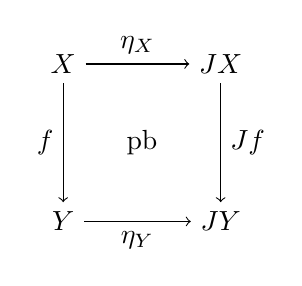
\begin{tikzpicture}
                \node (PB) at (0, 0) {pb};
                \node (X) at (-1, 1) {$X$};
                \node (JX) at (1, 1) {$\mathfrak{J}X$};
                \node (Y) at (-1, -1) {$Y$};
                \node (JY) at (1, -1) {$\mathfrak{J}Y$};
                \draw[->] (X) -- node[above]{$\eta_X$} (JX);
                \draw[->] (Y) -- node[below]{$\eta_Y$} (JY);
                \draw[->] (X) -- node[left]{$f$} (Y);
                \draw[->] (JX) -- node[right]{$\mathfrak{J}f$} (JY);
            \end{tikzpicture}
        \end{gather*}
    }

    \newdef{Super-differential cohesion}{\index{cohesion!super-differential}\index{solid|see{cohesion, super-differential}}
        Consider a differentially cohesive $(\infty,1)$-topos $\mathbf{H}_\text{bos}\rightarrow\mathbf{H}_\text{red}$. A super-differentially cohesive (or \textbf{solid}\footnote{This terminology stems from the fact that supergeometry is necessary for treating fermions, which are in turn responsible for solid matter physics.}) topos over $\mathbf{H}_\text{bos}$ is a differentially cohesive $(\infty,1)$-topos $\mathbf{H}\rightarrow\mathbf{H}_\text{red}$ equipped with an adjoint quadruple $(\mathrm{even}\dashv\iota_\text{sup}\dashv\Pi_\text{sup}\dashv\mathrm{Disc}_\text{sup}):\mathbf{H}\rightarrow\mathbf{H}_\text{bos}$ such that $\iota$ (and, hence, also $\mathrm{Disc}_\text{sup}$) is fully faithful.

        These structures give the following diagram of $(\infty,1)$-functors (again by uniqueness of adjoints and global sections):
        \begin{gather}
            \label{type:solid_diagram}
            \begin{tikzpicture}[baseline = 0]
                \node (A) at (0, 0) {$\mathbf{H}$};
                \node (B) at (3, 0) {$\mathbf{H}_\text{bos}$};
                \node (C) at (6, 0) {$\mathbf{H}_\text{red}$};
                \node (D) at (9, 0) {$\infty\mathbf{Grpd}$};
                \node (A1) at (0, 1) {$\phantom{\mathbf{H}}$};
                \node (B1) at (3, 1) {$\phantom{\mathbf{H}_\text{bos}}$};
                \node (C1) at (6, 1) {$\phantom{\mathbf{H}_\text{red}}$};
                \node (D1) at (9, 1) {$\phantom{\infty\mathbf{Grpd}}$};
                \node (A_1) at (0, -1) {$\phantom{\mathbf{H}}$};
                \node (B_1) at (3, -1) {$\phantom{\mathbf{H}_\text{bos}}$};
                \node (C_1) at (6, -1) {$\phantom{\mathbf{H}_\text{red}}$};
                \node (D_1) at (9, -1) {$\phantom{\infty\mathbf{Grpd}}$};
                \node (A_2) at (0, -2) {$\phantom{\mathbf{H}}$};
                \node (D_2) at (9, -2) {$\phantom{\infty\mathbf{Grpd}}$};
                \node (A2) at (0, 2) {$\phantom{\mathbf{H}}$};
                \node (B2) at (3, 2) {$\phantom{\mathbf{H}_\text{bos}}$};
                \node (C2) at (6, 2) {$\phantom{\mathbf{H}_\text{red}}$};
                \node (A3) at (0, 3) {$\phantom{\mathbf{H}}$};
                \node (B3) at (3, 3) {$\phantom{\mathbf{H}_\text{bos}}$};
                \draw[left hook->] (B) -- node[above]{$\mathrm{Disc}_\text{sup}$} (A);
                \draw[left hook->] (C) -- node[above]{$\mathrm{Disc}_\text{bos}$} (B);
                \draw[left hook->] (D) -- node[above]{$\mathrm{Disc}_\text{red}$} (C);
                \draw[->] (A1) -- node[above]{$\Pi_\text{sup}$} (B1);
                \draw[->] (B1) -- node[above]{$\Pi_\text{bos}$} (C1);
                \draw[->] (C1) -- node[above]{$\Pi_\text{red}$} (D1);
                \draw[->] (A_1) -- node[above]{$\Gamma_\text{sup}$} (B_1);
                \draw[->] (B_1) -- node[above]{$\Gamma_\text{bos}$} (C_1);
                \draw[->] (C_1) -- node[above]{$\Gamma_\text{red}$} (D_1);
                \draw[left hook->] (D_2) -- node[above]{$\mathrm{coDisc}$} (A_2);
                \draw[left hook->] (B2) -- node[above]{$\iota_\text{sup}$} (A2);
                \draw[left hook->] (C2) -- node[above]{$\iota_\text{bos}$} (B2);
                \draw[->] (A3) -- node[above]{$\mathrm{even}$} (B3);
            \end{tikzpicture}
        \end{gather}
    }

    \begin{property}[Solid modalities]
        As for cohesive and differentially cohesive topoi, the adjoint functors induce a set of (adjoint) modalities:
        \begin{gather}
            (\rightrightarrows\,\dashv\,\rightsquigarrow\,\dashv\mathrm{Rh}):=(\iota_\text{sup}\circ\mathrm{even}\dashv\iota_\text{sup}\circ\Pi_\text{sup}\dashv\mathrm{Disc}_\text{sup}\circ\Pi_\text{sup})\,.
        \end{gather}
        These are called the \textbf{fermionic}, \textbf{bosonic} and \textbf{rheonomic} modalities, respectively. Note that by Diagram~\ref{type:solid_diagram} a super-differentially cohesive topos also inherits the cohesive and differential modalities.
    \end{property}

    ?? COMPLETE (e.g.~work by Schreiber) ??

\section{Smooth spaces}\index{smooth!space}\label{section:smooth_spaces}

    In this section some generalizations of spaces that are better behaved when considering their properties as a whole are introduced. Before moving to the smooth setting, a bit of history will be given, starting from the ordinary topological setting.

    The first problem in the study of the global properties of spaces arose in algebraic topology. When consider mapping spaces it is sometimes useful to use the currying operation \[C(X\times Y,Z)\rightarrow C\big(X,C(Y,Z)\big).\] However, in general, this is not a homeomorphism, i.e.~currying does not define an adjunction and, therefore, $\mathbf{Top}$ is not Cartesian closed \ref{cat:closed}. This problem was treated by \textit{Steenrod} and others, and the solution was simply to restrict to a smaller class of better behaved spaces: the compactly generated Hausdorff spaces.\footnote{In practice this is not a problem since all interesting spaces, such as CW complexes, belong to this class.}

    Whilst studying varieties in algebraic geometry people experienced similar problems. For this reason \textit{Grothendieck} invented schemes (see Chapter \ref{chapter:alggeom} and Section \ref{section:schemes} in particular). The main takeaway of this approach was that ``it’s better to work with a nice category containing some nasty objects, than a nasty category containing only nice objects'' as \textit{Baez} phrases it succintly.

    The category $\mathbf{Diff}$ of finite-dimensional smooth manifolds suffers the same problems, namely the space of smooth functions $C^\infty(X,Y)$ is in general some kind of infinite-dimensional manifold and, hence, cannot be defined internally. It becomes even worse if one studies the mapping spaces between those. \textit{Kriegl} and \textit{Michor} have introduced a framework in which one can work safely, but the main problem with their solution is that not all spaces of interest are included. Certain other operations such as quotients and (co)limits are also not guaranteed to exist within that category.

\subsection{Fr\"olicher spaces}\index{Fr\"olicher space}

    \newdef{Fr\"olicher space}{
        A triple $(X,C_X,F_X)$ consisting of the following data:
        \begin{itemize}
            \item A set $X$,
            \item a set of curves $C_X\subseteq\mathbf{Set}(\mathbb{R},X)$, and
            \item a set of functionals $F_X\subseteq\mathbf{Set}(X,\mathbb{R})$.
        \end{itemize}
        These are required to satisfy the following closure and consistency conditions:
        \begin{enumerate}
            \item For all $c\in C_X$ and $f\in F_X$ the composite is smooth: $f\circ c\in C^\infty(\mathbb{R})$.
            \item If, given $c\in\mathbf{Set}(\mathbb{R},X)$, the composite $f\circ c\in C^\infty(\mathbb{R})$ for all functionals $f\in F_X$, then $c\in C_X$.
            \item If, given $f\in\mathbf{Set}(X,\mathbb{R})$, the composite $f\circ c\in C^\infty(\mathbb{R})$ for all curves $c\in C_X$, then $f\in F_X$.
        \end{enumerate}
        Morphisms of Fr\"olicher spaces are those functions that preserve curves, functionals and smoothness under composition.
    }

    \begin{property}
        The category of Fr\"olicher spaces is bicomplete and Cartesian closed.
    \end{property}

    \newdef{Topology}{
        Consider a Fr\"olicher space $(X,C_X,F_X)$. The \textbf{curvaceous topology} on $X$ is the final topology with respect to the curves $C_X$. The \textbf{functional topology} on $X$ is the initial topology with respect to the functionals $F_X$.
    }

    ?? COMPLETE (Isbell enveloppe / duality) ??

\subsection{Smooth sets}

    \newdef{Concrete site}{\index{concrete!site}
        Consider a site $(\mathbf{C},J)$. It is said to be concrete if
        \begin{enumerate}
            \item the functor $\mathbf{C}(\ast,-):\mathbf{C}\rightarrow\mathbf{Set}$ is faithful, and
            \item for every covering family $\{f_i:U_i\rightarrow U\}_{i\in I}\in J(U)$ the morphism
            \begin{gather}
                \bigsqcup_{i\in I}\mathbf{C}(\ast,f_i):\bigsqcup_{i\in I}\mathbf{C}(\ast,U_i)\rightarrow\mathbf{C}(\ast,U)
            \end{gather}
            is surjective.
        \end{enumerate}
    }

    \newdef{Concrete presheaf}{\index{concrete!sheaf}
        Consider a concrete site $(\mathbf{C},J)$. For every presheaf $X\in\mathbf{Psh}(\mathbf{C})$ and object $U\in\ob{C}$, denote by \[X_U:X(U)\rightarrow \mathbf{Set}\big(\mathbf{C}(\ast,U),X(\ast)\big)\] the adjunct of the restriction morphism \[X(U)\times\mathbf{C}(\ast,U)\rightarrow X(\ast).\] The presheaf $X$ is said to be concrete if for each $U\in\ob{C}$ the map $X_U$ is injective. This says that concrete presheaves are subobjects of presheaves of the form
        \begin{gather}
            U\mapsto\mathbf{Set}\big(\mathbf{C}(\ast,U),X(\ast)\big).
        \end{gather}
        This definition also agrees with Definition~\ref{topos:concrete_object}.
    }

    \begin{property}
        The category of sheaves on a concrete site is a local topos \ref{topos:local_topos}. The right adjoint $\func{\mathrm{coDisc}}{Set}{H}$ sends a set $A$ to the functor $U\mapsto\mathbf{Set}\big(\mathbf{C}(\ast,U),A\big)$.
    \end{property}
    This property allows to define concrete objects in any local topos in an alternative way (by slightly modifying Property~\ref{topos:characterization_embedding} to allow for separation instead of locality):
    \newdef{Concrete object}{\index{concrete!object}
        Consider a local geometric morphism $\Gamma:\mathbf{H}\rightarrow\mathcal{S}$. Consider the class $V$ of local isomorphisms with respect to $\Gamma$. An object in $\mathbf{H}$ is said to be concrete if it is $V$-separated, i.e.~its Yoneda embedding maps morphisms in $V$ to monos.
    }
    \begin{remark}
        Note that concrete sheaves carry two kinds of sheaf-theoretic information. On the one hand they are actual sheaves with respect to the Grothendieck topology of the underlying site and on the other hand they are separated presheaves with respect to the topology generated by global elements $\ast\rightarrow U$.
    \end{remark}

    \begin{property}[Concretification]\label{topos:concretification}
        Consider a local (1-)topos $\mathbf{H}$.\footnote{The restriction to ordinary topoi ensures that ordinary image factorization suffices. For higher topoi this would not be the case and higher image factorizations would be required.} Every topos has an epi/mono factorization giving rise to the image $\im(f)$ of a morphism $f\in\hom(\mathbf{H})$. The concretification of an object $X\in\ob{H}$ is given by the image $\im(\eta^\sharp_X)$. 
    \end{property}

    In the case of the site of Cartesian spaces, the following notion is obtained:
    \newdef{Diffeological space}{\index{diffeology}
        A diffeology on a set $X$ is a concrete sheaf $\mathcal{D}_X$ on $\mathbf{CartSp_{diff}}$ such that $\Gamma\mathcal{D}_X=X$.
    }

    \newadef{Diffeological space}{\index{diffeology}\index{plot}
        Let $X$ be a set. A diffeology $\mathcal{D}_X$ on $X$ is defined as a collection of functions $f:U\subseteq\mathbb{R}^n\rightarrow X$, called \textbf{plots}, satisfying the following conditions (where $U,V$ and $W$ are open sets):
        \begin{enumerate}
            \item $\mathcal{D}_X$ contains all constant functions.
            \item If $\{U_i\}_{i\in I}$ is an open cover of $U$ and if $f|_{U_i}\in\mathcal{D}_X$ for all $i\in I$, then $f\in\mathcal{D}_X$.
            \item If $f\in\mathcal{D}_X$ and $g:W\subseteq\mathbb{R}^m\rightarrow\dom(f)$ is smooth, then $f\circ g\in\mathcal{D}_X$.
        \end{enumerate}
        The set $X$ can be turned into a topological space by equipping it with the \textbf{$\mathcal{D}_X$-topology}, the final topology with respect to $\mathcal{D}_X$.
    }
    \remark{Note that in contrast to ordinary manifolds, the plots in a diffeology can have domains of different dimensions.}

    \newdef{Smooth map}{\index{smooth!function}
        \nomenclature[S_DiffSp]{$\mathbf{DiffSp}$}{category of diffeological spaces and smooth maps}
        Let $\mathcal{D}_X$ and $\mathcal{D}_Y$ be diffeological spaces. A map $g:X\rightarrow Y$ is said to be smooth if $g\circ f\in\mathcal{D}_Y$ for all $f\in\mathcal{D}_X$. The diffeological spaces together with their differentiable morphisms form a category $\mathbf{DiffSp}$.
    }

    \newdef{Chen space}{\index{Chen space}
        If the open sets in the definition of a diffeological space are replaced by convex sets, the notion of smooth spaces due to \textit{Chen} are obtained.
    }

    \begin{adefinition}[Manifold]\index{manifold}
        A diffeological space that is locally diffeomorphic to a Euclidean space. A map between manifolds is smooth in the diffeological sense if and only if it smooth in the sense of Definition \ref{manifolds:smooth_function}.
    \end{adefinition}

    There exist two trivial smooth structures:
    \begin{example}[Discrete structure]\index{discrete!smooth structure}
        The minimal smooth structure, i.e.~the one obtained by taking the plots to be the constant functions.
    \end{example}
    \begin{example}[Indiscrete structure]
        The maximal smooth structure, i.e.~the one obtained by taking all functions to be plots.
    \end{example}

    The notion of diffeological spaces can be further generalized by passing to the full sheaf topos on Cartesian spaces:
    \newdef{Smooth set}{\index{smooth!set}
        \nomenclature[S_Cinf]{$\mathbf{C^\infty}$, $\mathbf{SmoothSet}$}{category of smooth sets}
        \begin{gather}
            \mathbf{SmoothSet}:=\mathbf{Sh(CartSp_{diff})}.
        \end{gather}
        The topology on this site is generated by the coverage of differentiably good covers \ref{manifold:good_cover} (in fact, this topology coincides with the usual one consisting of open covers). The category of smooth sets is also denoted by $\mathbf{C^\infty}$.

        To phrase this in the sense of Section~\ref{section:cohesion}, smooth sets form a cohesive topos over $\mathbf{Set}$, where $\mathrm{Disc}$ and $\mathrm{coDisc}$ assigns the discrete and codiscrete structures from the preceding examples, respectively. Moreover, this cohesive topos satisfies the Nullstellensatz~\ref{topos:nullstellensatz}.
    }

    \begin{property}
        There exists an adjunction
        \begin{gather}
            \mathbf{Top}\adj{\mathrm{top}}{\mathrm{diff}}\mathbf{C^\infty}.
        \end{gather}
        The right adjoint endows a topological space $X$ with the smooth structure for which every continuous map $U\rightarrow X$ is a plot. Its left adjoint sends a smooth space to the topological space equipped with the finest topology for which all plots become continuous maps.
    \end{property}

    \begin{property}\label{topos:discrete_smooth_sets}
        The adjunction $\Pi_0\dashv\mathrm{Disc}$ exhibits the discrete smooth sets, i.e.~the constant sheaves, as the reflective subcategory on $\mathbb{R}$-local objects (see also Property~\ref{model:reflective_localization}).
    \end{property}

    The subcategory of diffeological spaces, the concrete smooth sets, are those that have an underlying set of points. A common example of smooth sets that do not have such an underlying set is given by de Rham spaces:
    \begin{example}[Differential forms]
        Consider the $k^{th}$ de Rham functor $\Omega^k$ on the category $\mathbf{Diff}$. This functor assigns to every smooth manifold its space of differential $k$-forms. Locally defined forms can be glued together if they agree on intersections, i.e.~they satisfy the sheaf condition. This shows that $\Omega^k$ defines a smooth set, albeit one that is far from an ordinary smooth manifold. It is called the (universal) moduli space of differential $k$-forms. Note, however, that for a given smooth set $X\in\mathbf{C^\infty}$, the plots of $[X,\Omega^k]$ correspond to differential $k$-forms on the product $\mathbb{R}^n\times X$ and not to $\mathbb{R}^n$-parametrized forms on $X$. For the latter, one should consider the concretification $\mathrm{conc}[X,\Omega^k]$.

        One can go even further and characterize specific geometric structures in terms of this functor. Consider for example the subfunctor $\Omega^2_\mathrm{cl}$ that assigns closed two-forms. This also defines a smooth space and, hence, one can consider the slice category $\mathbf{C^\infty}/\Omega^2_\mathrm{cl}$. It is not hard to show that the category $\mathbf{SpMfd}$ of symplectic manifolds admits an embedding into this slice category.
    \end{example}
    \begin{property}[Universal differential forms]
        Consider the differential $n$-form
        \begin{gather}
            \omega_\text{univ}\in\Omega^n(\Omega^n)
        \end{gather}
        modulated by the identity morphism on $\Omega^n$, the universal differential $n$-form. Every differential $n$-form on any smooth set can be obtained as a pullback of $\omega_\text{univ}$.
    \end{property}

    \begin{example}[Path space]
        Since every topos is Cartesian closed, all internal homs exist. The path space of a smooth set $X$ is defined as
        \begin{gather*}
            \mathbf{P}X := [\mathbb{R},X]\,.
        \end{gather*}
        Its underlying set is given by the set of smooth plots (trajectories): $\Gamma[\mathbb{R},X]\cong\mathbf{C^\infty}(\mathbb{R},X)$.

        Analogously, the internal hom out of $X$ gives the moduli space of smooth functions on $X$:
        \begin{gather}
            \mathbf{C^\infty}(X) := [X,\mathbb{R}]\,.
        \end{gather}
    \end{example}

    \newdef{Transgression}{\index{transgression}
        Consider a smooth set $X\in\ob{C^\infty}$. Transgression of differential forms on $X$ along a compact $k$-manifold $\Sigma$ is defined as the composite:
        \begin{gather}
            \tau_\Sigma\omega := \int_\Sigma[\Sigma,\omega]:[\Sigma,X]\rightarrow[\Sigma,\Omega^n]\xrightarrow{\int_\Sigma}\Omega^{n-k}\,.
        \end{gather}
        An alternative approach uses a pullback along the evaluation morphism $\mathrm{ev}_\Sigma:\Sigma\times[\Sigma,X]\rightarrow X$.
    }
    \begin{property}
        If the compact $k$-manifold $\Sigma$ has a boundary, transgression of closed differential forms along $\Sigma$ and $\partial\Sigma$ is related by the de Rham differential:
        \begin{gather}
            \tau_{\partial\Sigma}(\omega) = (-1)^{k+1}d\tau_\Sigma\omega
        \end{gather}
        for all $\omega:X\rightarrow\Omega^n_\text{cl}$.
    \end{property}

\subsection{Smooth algebras}

    \newdef{Smooth algebra}{\index{smooth!algebra}
        \nomenclature[S_CSmAlg]{$\mathbf{C^\infty Ring},\mathbf{C^\infty Alg}$}{category of smooth algebras}
        For any smooth manifold $M$, the algebra of smooth functions can be obtained as a hom-object: \[C^\infty(M):=C^\infty(M,\mathbb{R})=\mathbf{Diff}(M,\mathbb{R}).\] Since hom-functors are (finite) product-preserving, the multiplication $C^\infty(M)\times C^\infty(M)\rightarrow C^\infty(M)$ can be seen to be induced by the multiplication on $\mathbb{R}$:
        \begin{gather}
            C^\infty(M, \mathbb{R}\times\mathbb{R})\cong C^\infty(M)\times C^\infty(M).
        \end{gather}
        Furthermore, the hom-functor is covariant in the second argument and, hence, defines a copresheaf on the category $\mathbf{CartSp_{diff}}$. Generalizing this situation, smooth algebras are defined as finite product-preserving copresheaves on $\mathbf{CartSp_{diff}}$. This (functor) category is denoted by $\mathbf{C^\infty Alg}$.
    }
    \newdef{Underlying algebra}{
        Given a smooth algebra $R\in\mathbf{C^\infty Alg}$, its underlying algebra $U(R)$ is defined as the set $R(\mathbb{R})$ equipped with the canonically induced ring operations.
    }

    \newdef{Finitely generated smooth algebra}{
        Since ordinary $R$-algebras are finitely generated if and only if they are of the form $R[x_1,\ldots,x_k]/I$ for some integer $k\in\mathbb{N}$ and some ideal $I$, a smooth algebra is said to be finitely generated if it is of the form $C^\infty(\mathbb{R}^n)/I$ for some $n\in\mathbb{N}$ and some ideal $I$ in the underlying algebra.
    }
    \newdef{Smooth locus}{\index{smooth!locus}
        Let $\mathbf{C^\infty Alg^{fin}}$ denote the category of finitely generated smooth algebras. The category of \textbf{smooth loci} is defined as $(\mathbf{C^\infty Alg^{fin}})^{op}$. The smooth locus corresponding to a smooth algebra $R$ is often denoted by $\ell R$.
    }

\subsection{Supergeometry}

    In this section the definition of smooth spaces (and sets) is generalized to the odd (fermionic) sector, i.e.~``super smooth sets'' will be defined. It gives an explicit example of a super-differentially cohesive $(\infty,1)$-topos.

    \newdef{Superscheme}{\index{super-!scheme}
        The category of affine superschemes is defined as the opposite of the category of supercommutative superalgebras, the commutative monoids internal to $\mathbf{sVect}$:
        \begin{gather}
            \mathbf{Aff(sVect)} := \mathbf{sCAlg}^{op} := \mathbf{CMon(sVect)}\,.
        \end{gather}
        More generally, one can define affine schemes internal to any symmetric monoidal category.
    }

    \newdef{Infinitesimally thickened space}{\index{thickened space}\label{hdg:infinitesimal_thickening}
        \nomenclature[S_FormalCartSp]{$\mathbf{FormalCartSp_{diff}}$}{category of infinitesimally thickened Euclidean spaces}
        First, consider a point $\mathbb{R}^0$. Its infinitesimal thickening should be a space such that every function that vanishes at the origin is actually nilpotent (this is essentially a version of the Kock-Lawvere axiom \ref{synth:kock_lawvere_axiom}):
        \begin{gather}
            \mathbb{D} := \mathrm{Spec}(A)\,,
        \end{gather}
        where $A:=\mathbb{R}\oplus V$ for $V$ a finite-dimensional nilpotent ideal.\footnote{Algebras of this form are also called \textbf{Weil algebras} or \textbf{local Artin algebras}.} A Euclidean space can be infinitesimally thickened by taking the product with $\mathbb{D}$ or, at the algebraic level, by taking the tensor product with $A$. A morphism of such spaces is defined by an $R$-algebra morphism between their associated algebras. These form the category $\mathbf{FormalCartSp_{diff}}$.
    }
    \begin{definition}[Superpoint]\index{super-!point}\index{super-!space}
        A space of the form $\mathrm{Spec}(\Lambda^\bullet\mathbb{R}^n)$. This is often denoted by $\mathbb{R}^{0\mid n}$. The \textbf{super-Euclidean space} $\mathbb{R}^{m\mid n}$ is obtained as the product of an ordinary Euclidean space $\mathbb{R}^m$ and the superpoint $\mathbb{R}^{0\mid n}$, i.e.~its algebra of smooth functions is $C^\infty(\mathbb{R}^m)\otimes\Lambda^\bullet\mathbb{R}^n$.\footnote{Compare this to the definition of supermanifolds~\ref{hdg:supermanifold}.}
    \end{definition}
    \begin{example}[First-order neighbourhood]
        For $A=\mathbb{R}[\varepsilon]/\varepsilon^2$, the definition of an infinitesimal thickening recovers the first-order infinitesimal neighbourhood of Definition~\ref{synth:infinitesimal_line}: $\mathbb{D}^1:=\mathrm{Spec}(\mathbb{R}[\varepsilon]/\varepsilon^2)$. The morphism dual to the mapping implied by the Kock-Lawvere axiom \ref{synth:kock_lawvere_axiom} gives an inclusion map $\mathbb{D}^1\hookrightarrow\mathbb{R}^1$. (This example can easily be generalized to $k^{th}$-order neighbourhoods.) This algebra is the algebra of functions on the even part of the superplane:
        \begin{gather}
            \mathcal{O}\big(\mathrm{even}\,\mathbb{R}^{0\mid 2}\big)\cong\mathbb{R}[\varepsilon]/\varepsilon^2\,.
        \end{gather}
    \end{example}

    \begin{property}[Morphisms]
        First, consider the morphisms from a Euclidean space into an infinitesimal neighbourhood $\mathbb{D}^k$. Since such morphisms are dual to algebra morphisms, one should consider morphisms of the form $\mathbb{R}[\varepsilon]/\varepsilon^{k+1}\rightarrow C^\infty(\mathbb{R}^n)$. However, being an algebra morphism implies that $f(1)=1$ and that nilpotents are mapped to nilpotents. The algebra of smooth functions on a Euclidean space does not contain nilpotents and, hence, there exists a unique function into an infinitesimal neighbourhood (the one that factorizes through the one-point set).

        For morphisms out of (first-order) infinitesimal neighbourhoods one obtains the property, known from synthetic geometry, that morphisms of the form $\mathbb{R}^n\times\mathbb{D}^1\rightarrow\mathbb{R}^n$ correspond to vector fields on $\mathbb{R}^n$ exactly when the postcomposition with the inclusion $\mathbb{R}^n\hookrightarrow\mathbb{R}^n\times\mathbb{D}^1$ is the identity.
    \end{property}

    \newdef{Formal smooth set}{\index{formal set}\index{smooth|seealso{formal}}\index{Cahiers topos}\index{plot}
        A sheaf on the site of infinitesimally thickened Euclidean spaces, where covers are of the form $\{U_i\times\mathrm{Spec}(A)\mid U_i\subseteq\mathbb{R}^n\}$, for $A$ a commutative (hence, even) algebra. The category of formal smooth sets or, equivalently, the sheaf topos on $\mathbf{FormalCartSp_{diff}}$ is also called the \textbf{Cahiers topos}. The sets in the image of a formal smooth set $X$ are called the sets of \textbf{plots} of $X$ and can be interpreted as sets of functions into $X$ (in analogy with the definition of smooth sets).
    }

    \newdef{Super smooth set}{\index{smooth!set}\index{Dubuc}
        By combining infinitesimal thickenings and superpoints, the category $\mathbf{SuperFormalCartSp_{diff}}$ is obtained. A sheaf on this category is called a super smooth set. Since \textit{Dubuc} introduced the Cahiers topos, the category of super smooth sets is sometimes called the \textbf{super-Dubuc topos}.
    }

    \begin{property}[Cohesion]
        The full subcategory inclusion $\mathbf{CAlg}\hookrightarrow\mathbf{sCAlg}$ is part of an adjoint cylinder, where the left and right adjoints are given by projection onto the even part and quotienting out the odd part:
        \begin{gather}
            \mathrm{even}\dashv\,\iota\dashv-/(-)_\mathrm{odd}\,,
        \end{gather}
        where $(-)_\mathrm{odd}$ indicates that the ideal generated by odd elements is quotiented out, i.e.~every term containing at least one odd factor is set to zero. These define canonical functors, $\mathrm{even}$ and $\Pi_\text{sup}$, from the category of affine superschemes to affine schemes (and, hence, also between the larger categories of superschemes and schemes). Moreover, the inclusion of affine schemes into infinitesimally thickened spaces also admits a right adjoint given by reduction: $\Pi_\text{inf}(\mathbb{R}^n\times\mathbb{D}):=\mathbb{R}^n$.

        These in turn induce a system of ajunctions between the sheaf topos of smooth sets, the Cahiers topos and the super-Dubuc topos, characterizing them as a cohesive, elastic and solid topoi, respectively:
        \begin{gather}
            \begin{tikzpicture}[baseline = 0]
                \node[align=center] (A) at (0, 0) {\textbf{Super}\\\textbf{Smooth}\\\textbf{Set}};
                \node[align=center] (B) at (4, 0) {\textbf{Formal}\\\textbf{Smooth}\\\textbf{Set}};
                \node (C) at (8, 0) {$\mathbf{C^\infty}$};
                \node (D) at (12, 0) {$\mathbf{Set}$};
                \node (A1) at (0, 1) {$\phantom{\mathbf{H}}$};
                \node (B1) at (4, 1) {$\phantom{\mathbf{H}_\text{bos}}$};
                \node (C1) at (8, 1) {$\phantom{\mathbf{H}_\text{red}}$};
                \node (D1) at (12, 1) {$\phantom{\infty\mathbf{Grpd}}$};
                \node (A_1) at (0, -1) {$\phantom{\mathbf{H}}$};
                \node (B_1) at (4, -1) {$\phantom{\mathbf{H}_\text{inf}}$};
                \node (C_1) at (8, -1) {$\phantom{\mathbf{H}_\text{red}}$};
                \node (D_1) at (12, -1) {$\phantom{\infty\mathbf{Grpd}}$};
                \node (A_2) at (0, -2) {$\phantom{\mathbf{H}}$};
                \node (D_2) at (12, -2) {$\phantom{\infty\mathbf{Grpd}}$};
                \node (A2) at (0, 2) {$\phantom{\mathbf{H}}$};
                \node (B2) at (4, 2) {$\phantom{\mathbf{H}_\text{inf}}$};
                \node (C2) at (8, 2) {$\phantom{\mathbf{H}_\text{red}}$};
                \node (A3) at (0, 3) {$\phantom{\mathbf{H}}$};
                \node (B3) at (4, 3) {$\phantom{\mathbf{H}_\text{inf}}$};
                \draw[left hook->] (B) -- node[above]{$\mathrm{Disc}_\text{sup}$} (A);
                \draw[left hook->] (C) -- node[above]{$\mathrm{Disc}_\text{inf}$} (B);
                \draw[left hook->] (D) -- node[above]{$\mathrm{Disc}_\text{red}$} (C);
                \draw[->] (A1) -- node[above]{$\Pi_\text{sup}$} (B1);
                \draw[->] (B1) -- node[above]{$\Pi_\text{inf}$} (C1);
                \draw[->] (C1) -- node[above]{$\Pi_\text{red}$} (D1);
                \draw[->] (A_1) -- node[above]{$\Gamma_\text{sup}$} (B_1);
                \draw[->] (B_1) -- node[above]{$\Gamma_\text{inf}$} (C_1);
                \draw[->] (C_1) -- node[above]{$\Gamma_\text{red}$} (D_1);
                \draw[left hook->] (D_2) -- node[above]{$\mathrm{coDisc}$} (A_2);
                \draw[left hook->] (B2) -- node[above]{$\iota_\text{sup}$} (A2);
                \draw[left hook->] (C2) -- node[above]{$\iota_\text{inf}$} (B2);
                \draw[->] (A3) -- node[above]{$\mathrm{even}$} (B3);
            \end{tikzpicture}
        \end{gather}
        The top four functors in every column are obtained by Kan extension from the functors between affine spaces (Property~\ref{cat:kan_quadruple}). The others follow from uniqueness and composition properties of adjoints and the fact that the coverages on $\mathbf{SuperSmoothSet}$ and $\mathbf{FormalSmoothSet}$ are trivial along infinitesimal thickenings and odd dimensions.
    \end{property}

    By the general theory of cohesive topoi, the diagram of adjunctions induce a another diagram of adjoint modalities. These are listed below.
    \newdef{Fermionic modalities}{
        The adjoint cylinder induced by the inclusion $\mathbf{CAlg}\hookrightarrow\mathbf{sCAlg}$ in turn gives rise to the adjoint modalities
        \begin{gather}
            \overrightarrow{\overrightarrow{(-)}}\dashv\overset{\rightsquigarrow}{(-)}\,.
        \end{gather}
        The left adjoint sends a super smooth set to its ``bifermionic'' space, where only paired fermions occur. The right adjoint sends a super smooth set to its underlying bosonic space and might, therefore, be called the \textbf{bosonic modality}.

        Moreover, since these modalities come from an adjoint quadruple, a further right adjoint exists. The rheonomy modality corresponds to localization at the superpoint:
        \begin{gather}
            \mathrm{Rh}\cong L_{\mathbb{R}^{0\mid1}}\,,
        \end{gather}
        akin to Property~\ref{topos:discrete_smooth_sets}.
    }

    The following definition is dual to \ref{algebra:reduction}:
    \newdef{Reduction}{\index{reduction}\index{infinitesimal}
        By Property~\ref{topos:differential_modalities}, $\mathbf{SuperSmoothSet}$ admits differential modalities to both $\mathbf{FormalSMoothSet}$ and $\mathbf{SmoothSet}$. The reduction modality $\mathfrak{R}$ simply drops all infinitesimal directions, both even- and odd-graded:
        \begin{gather}
            \mathfrak{R}(\mathbb{R}^{m\mid n}\times\mathbb{D}) = \mathbb{R}^m\,.
        \end{gather}

        The \textbf{infinitesimal neighbourhood} (to arbitrary order) of a formal smooth subset $Y\hookrightarrow X$ is defined by taking its plots to be those plots of $X$ for which the reductions factorize through plots of $Y$.
    }
    \newdef{Shape modality}{\index{modality!shape}\index{shape}\index{de Rham!shape}
        The \textbf{(infinitesimal) shape} or \textbf{de Rham shape} $\mathfrak{J}X$ of a super smooth set $X$ is given, throught duality/adjointness, by the super smooth set obtained by reducing the plots of $X$:
        \begin{gather}
            \mathfrak{J}X(U) := X(\mathfrak{R}(U)).
        \end{gather}
        This construction identifies all infinitesimally close points.
    }

    \newdef{Tangent bundle}{\index{tangent!bundle}
        Consider a super smooth set $X\in\ob{SuperSmoothSet}$. Its tangent bundle is given by the internal hom out of the infinitesimal disk:
        \begin{gather}
            TX := [\mathbb{D}^1,X]\,.
        \end{gather}
        Precomposition by the unique global element of $\mathbb{D}^1$ gives the bundle projection $TX\rightarrow X$. Analogously, the internal hom out of the superpoint gives the odd tangent bundle (see also Definition~\ref{hdg:odd_tangent_bundle}):
        \begin{gather}
            \Pi TX := [\mathbb{R}^{0\mid1},X]\,.
        \end{gather} 
    }


    \newdef{Local diffeomorphism\footnotemark}{\index{local!diffeomorphism}
        Recall definition~\ref{topos:formally_etale}. In the setting of super smooth sets this is equivalent to a morphism $f:X\rightarrow Y$ such that the thickened plots of $X$ can be identified with those of $Y$ whose reduction comes from a Euclidean plot of $X$. Equivalently, by taking internal homs, a morphism of super smooth sets is formally \'etale if and only if
        \begin{gather*}
            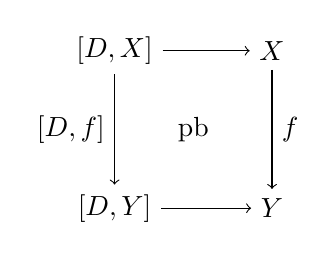
\begin{tikzpicture}
                \node (PB) at (0, 0) {pb};
                \node (X) at (-1, 1) {$[\mathbb{D},X]$};
                \node (JX) at (1, 1) {$X$};
                \node (Y) at (-1, -1) {$[\mathbb{D},Y]$};
                \node (JY) at (1, -1) {$Y$};
                \draw[->] (X) -- (JX);
                \draw[->] (Y) -- (JY);
                \draw[->] (X) -- node[left]{$[\mathbb{D},f]$} (Y);
                \draw[->] (JX) -- node[right]{$f$} (JY);
            \end{tikzpicture}
        \end{gather*}
        is a pullback square for all infinitesimally thickened (super)points. By taking $\mathbb{D}=\mathbb{D}^1$, the inverse function theorem~\ref{bundle:inverse_function_theorem} can be recovered.

        This can also be related to the definition in commutative algebra (and dually, that in algebraic geometry) as follows. The shape modality is right adjoint to the reduction modality. Sending a ring (extension) to its representable presheaf and using the Yoneda lemma gives
        the diagram
        \begin{gather*}
            \begin{tikzpicture}
                \node (PB) at (0, 0) {pb};
                \node (X) at (-2, 1) {$\mathbf{CRing}(A,B)$};
                \node (JX) at (2, 1) {$\mathbf{CRing}(A,B/I)$};
                \node (Y) at (-2, -1) {$\mathbf{CRing}(R,B)$};
                \node (JY) at (2, -1) {$\mathbf{CRing}(R,B/I)$};
                \draw[->] (X) -- (JX);
                \draw[->] (Y) -- (JY);
                \draw[->] (X) -- (Y);
                \draw[->] (JX) -- (JY);
            \end{tikzpicture}
        \end{gather*}
        This square being a pullback exactly corresponds to the lifting condition in Definition \ref{algebra:formally_etale}.
    }

    \begin{property}\label{hdg:bosonic_formally_etale}
        Local diffeomorphisms are preserved by the bosonic modality: If $f$ is formally \'etale, so is $\overset{\rightsquigarrow}{f}$.
    \end{property}

    \newadef{Smooth manifold}{\index{manifold}
        A diffeological space (in its incarnation as a formal smooth set) equipped with a family of local diffeomorphisms from Euclidean spaces (also regarded as formal smooth sets) such that every point of the space lies in the image of at least one such morphism and such that the final topology induced by the plots of the smooth set is paracompact Hausdorff.
    }

    \newdef{$V$-manifold}{
        Consider a group object $V\in\mathbf{SuperSmoothSet}$. A $V$-manifold is a super smooth set $X$ equipped with a span
        \begin{gather*}
            \begin{tikzpicture}
                \node (U) at (0, 0) {$U$};
                \node (V) at (-2, -2) {$V$};
                \node (X) at (2, -2) {$X$};
                \draw[->] (U) -- node[above left]{\'et} (V);
                \draw[->] (U) -- node[above right]{\'et, epi} (X);
            \end{tikzpicture}
        \end{gather*}
    }
    \newdef{Supermanifold}{\index{super-!manifold}
        A supermanifold of \textbf{(super)dimension} $(m\mid n)$ is a super smooth set $X$ equipped with a formally \'etale epimorphism $\sqcup_{i\in I}\mathbb{R}^{m\mid n}\rightarrow X$ for some index set $I$.

        Using the notion of supermanifold, one can also define super fibre bundles (and other common notions from differential geometry). Given such a bundle $E\rightarrow M$, its (super)space of sections is the fibre product
        \begin{gather*}
            \Gamma(E) := [M,E]\times_{[M,M]}\mathcal{Y}\{\mathbbm{1}_M\}\,.
        \end{gather*}
    }

    \begin{property}
        By Property~\ref{hdg:bosonic_formally_etale} above, the bosonic space underlying a $V$-manifold is a $\overset{\rightsquigarrow}{V}$-manifold.
    \end{property}

\section{Gauge theory}

    Recall the notions of Chapter~\ref{chapter:topos}, in particular the notions of stacks and higher topoi. The $(\infty,1)$-category of smooth $\infty$-stacks can be described in terms of (left Bousfield) localization of a suitable presheaf category by Lurie's theorem~\ref{model:lurie_presentation}.

    The first possibility is the category of $\infty$-presheaves on $\mathbf{Diff}$ with the localization at open covers. The second possibility is the dense subsite $\mathbf{CartSp_{diff}}$ with localization at good open covers. Both will result in a \v{C}ech model structure \ref{topos:cech_model_structure}. However, the specific properties will differ.

    \begin{example}[Classifying stacks]
        Consider the example of a Lie group $G$ and its classifying stack $\mathbf{B}G$. In the first model structure, the mapping space $\mathbf{H}(M,\mathbf{B}G)$, for $M$ a smooth manifold, is just presented\footnote{This means the homotopy-invariant hom-object in the underlying presheaf category, where the domain is replaced by a cofibrant object and the codomain by a fibrant object.} by $\hom(M,\mathbf{B}G)$, since $M$ is cofibrant as a representable presheaf and $\mathbf{B}G$ is fibrant by gluing over covers. So mapping spaces $\mathbf{H}(M,\mathbf{B}G)$ are just given by groupoids of $G$-bundles over $M$.

        On the subsite $\mathbf{CartSp}_\mathrm{diff}$, the presheafs represented by manifolds are not cofibrant anymore. However, \v{C}ech nerves of open covers give a cofibrant replacement. On the other hand, over Cartesian spaces the stacks are trivial and can be presented as action groupoids $\ast/\!\!/G$ (the ordinary deloopings). A fibrant replacement is given by the presheaf
        \begin{gather}
            U\mapsto N_\Delta\big(\ast/\!\!/C^\infty(U,G)\big).
        \end{gather}
        This presheaf is also equivalent to the groupoid of $G$-bundles (over $U$). The derived mapping space in this situation is given by (normalized) $G$-valued \v{C}ech cocycles.
    \end{example}

\section{Higher Lie theory}

    In this section some notions about groups, Lie groups and groupoids (Sections \ref{section:groups}, \ref{section:lie_groups} and \ref{section:groupoids}) are extended the setting of higher category theory.

    \newdef{Lie groupoid\footnotemark}{\index{Lie!groupoid}\label{hdg:lie_groupoid}
        \footnotetext{In a similar way one could define \textit{topological groupoids, \'etal\'e groupoids}, ...}
        A groupoid internal to $\mathbf{Diff}$.
    }
    \begin{remark}
        Note that Definition \ref{cat:internal_category} requires the existence of pullbacks. In the category $\mathbf{Diff}$ this is equivalent to assuming that the source and target morphisms are (surjective) submersions.

        In the Ehresmannian approach the manifold of composable morphisms $D_1\times_{D_0}D_1$ is given as part of the data. Hence, no further assumptions have to be made about the source and target morphisms.
    \end{remark}

    \newdef{Lie algebroid}{\index{Lie!algebroid}\index{anchor}\label{hdg:lie_algebroid}
        A vector bundle $\pi:E\rightarrow M$ together with a morphism $\rho:E\rightarrow TM$, called the \textbf{anchor map}, and a Lie bracket on $\Gamma(E)$ such that the following Leibniz-type property is satisfied:
        \begin{gather}
            [X,fY] = f[X,Y] + \rho(X)(f)Y.
        \end{gather}
        This property also implies that $\rho$ preserves the Lie bracket:
        \begin{gather}
            \rho([X,Y]) = [\rho(X),\rho(Y)].
        \end{gather}
        In local coordinates $x^i$ and for a local basis of sections $s_\alpha$, the bracket and anchor can be expressed in terms of structure functions:
        \begin{align}
            \rho(s_\alpha) &= R^i_\alpha\partial_i\,,\\
            [s_\alpha,s_\beta] &= C^\gamma_{\alpha\beta}(x)s_\gamma.
        \end{align}
        The Lie algebroid properties then imply the following conditions on these structure functions:
        \begin{gather}
            R^j_\alpha\pderiv{R^i_\beta}{x^j}-R^j_\beta\pderiv{R^i_\alpha}{x^j} = R^i_\gamma C^\gamma_{\alpha\beta}
        \end{gather}
        and
        \begin{gather}
            R^i_\alpha\pderiv{C^\kappa_{\beta\gamma}}{x^i}+C^\kappa_{\alpha\mu}C^\mu_{\beta\gamma} + (\alpha\leftrightarrow\beta\leftrightarrow\gamma) = 0.
        \end{gather}
    }
    \begin{example}[Tangent Lie algebroid]\index{pair!groupoid}
        The tangent bundle over a smooth manifold is a Lie algebroid with $\rho=\mathbbm{1}_{TM}$.

        Consider the \textbf{pair groupoid} or \textbf{codiscrete groupoid} $\mathbf{M\times M}$:
        \begin{itemize}
            \item\textbf{Objects}: $M$, and
            \item\textbf{Morphisms}: $M\times M$, i.e.~between every two points there exists a unique morphism.
        \end{itemize}
        Both the fundamental groupoid $\mathbf{\Pi_1}(M)$ of Definition \ref{topology:fundamental_groupoid} and the pair groupoid $\mathbf{M\times M}$ \textit{integrate} the tangent Lie algebroid.
    \end{example}

    ?? ADD LIE INTEGRATION OF ALGEBROIDS ??

    One can generalize the dual construction of $L_\infty$-algebras even further:
    \newdef{$L_\infty$-algebroid}{
        Consider the construction \ref{hda:l_infinity_bis} of the Chevalley-Eilenberg algebra for a $L_\infty$-algebra. By replacing the base field by a smooth algebra $C^\infty(M)$ for some smooth manifold $M$ and the (graded) vector space $V$ by a module of sections $\Gamma(E)$ of a (graded) vector bundle $E\rightarrow M$, one obtains the notion of a $L_\infty$-algebroid.
    }
    \begin{property}
        $L_\infty$-algebras can be recovered by considering the special case $M=\{\ast\}$.
    \end{property}

    \begin{example}[de Rham complex]\index{de Rham!complex}
        Consider the tangent algebroid of a smooth manifold $M$. The associated Chevalley-Eilenberg complex is equivalent to the de Rham complex $\Omega^\bullet(M)$.
    \end{example}

\section{Weak groups}

    \newdef{Weak 2-group}{\index{group!categorical}\index{2-!group}
        Let $(\mathbf{C},\otimes,\mathbf{1})$ be a monoidal category. This category is called a weak 2-group or \textbf{categorical group} if it satisfies the following conditions:
        \begin{enumerate}
            \item All morphisms are invertible.
            \item Every object is weakly invertible with respect to the monoidal structure.
        \end{enumerate}
        By Property \ref{cat:monoidal_or_2} one can equivalently define a weak 2-group as a 2-category with a single object, weakly invertible 1-morphisms and invertible 2-morphisms.

        The definition of a weak 2-group can be strengthened to that of a \textbf{coherent 2-group} (sometimes called a \textbf{gr-category}), where the isomorphisms $x\otimes x^{-1}\rightarrow\mathbf{1}$ and $x^{-1}\otimes x\rightarrow\mathbf{1}$ glue together to form an adjoint equivalence.
    }
    \begin{example}[Automorphism 2-group]
        Consider a 2-category $\mathbf{C}$. For every object $c\in\ob{C}$, the automorphism category $\mathbf{Aut}(c)$ of autoequivalences of $c$ and invertible 2-morphisms between them forms a coherent 2-group.\footnote{Relaxing the objects to weakly invertible 1-morphisms gives a weak 2-group.}
    \end{example}

    \newdef{2-groupoid}{\index{2-!groupoid}
        A 2-groupoid is a 2-category in which all 1-morphisms are invertible and every 2-morphisms has a ``vertical'' inverse. (The ``horizontal'' inverse can be constructed from the other ones.)
    }

    \newdef{Strict 2-group}{
        A (strict) 2-group is defined as a (strict) 2-groupoid with only one object. From this it follows that the set of 1-morphisms forms a group and so does the set of 2-morphisms under horizontal composition. However, the 2-morphisms do not form a group under vertical composition because the sources/targets may not match.

        This definition is equivalent to the following internal version. A (strict) 2-group is a group object in $\mathbf{Cat}$ or an internal category in $\mathbf{Grp}$. If $\mathbf{Grp}$ is replaced by $\mathbf{Lie}$, the notion of a (strict) Lie 2-group is obtained.
    }
    \newdef{$\infty$-groupoid}{
        A $\infty$-category in which all morphisms are invertible. This is equivalent to a $(\infty,0)$-category in the language of $(n,r)$-categories.
    }

    \begin{property}[Lie crossed modules]\index{module!crossed}\index{differential!crossed module}
        The 2-category of (strict) 2-groups is biequivalent to the 2-category of (Lie) crossed modules \ref{group:crossed_module}. Given a 2-group $\mathcal{G}$, a crossed module is obtained as follows:
        \begin{itemize}
            \item $G:=\ob{\mathcal{G}}$,
            \item $H:=\{h\in\mathrm{hom}(\mathcal{G})\mid\mathfrak{s}(f)=e\}$,
            \item $t(h):=\mathfrak{t}(h)$, and
            \item $\alpha(g)h := \mathbbm{1}_gh\mathbbm{1}_g^{-1}$,
        \end{itemize}
        where $\mathfrak{s},\mathfrak{t}$ are the source and target morphisms in $\mathcal{G}$.

        To every Lie crossed module one can also assign a \textbf{differential crossed module}. This consists of the following data:
        \begin{itemize}
            \item two Lie algebras $\mathfrak{g},\mathfrak{h}$,
            \item a Lie algebra morphism $\partial:\mathfrak{h}\rightarrow\mathfrak{g}$, and
            \item a Lie algebra morphism $\rho:\mathfrak{g}\rightarrow\text{Der}(\mathfrak{h})$.
        \end{itemize}
        The equivariance and Peiffer conditions induce similar conditions for the above data:
        \begin{itemize}
            \item $\partial(\rho(h)g) = [h,\partial g]$, and
            \item $\rho(\partial h)(h') = [h,h']$\,,
        \end{itemize}
        where $g\in\mathfrak{g}$ and $h,h'\in\mathfrak{h}$. The biequivalence of crossed modules and strict 2-groups induces a biequivalence of differential crossed modules and strict Lie 2-algebras.
    \end{property}

    \begin{example}[Automorphism 2-group]
        Given a Lie group $H$, one can construct a crossed module with $G:=\Aut(H)$, $t$ assigning inner automorphisms (conjugations) and $\alpha$ the obvious map. The associated 2-group $\mathbf{Aut}(H)$ is the automorphism 2-group of $H$ of the delooping $\mathbf{B}H$.
    \end{example}

    \newdef{Exponentiable group}{\index{exponentiable}
        A smooth group for which every smooth function $f:[0,1]\rightarrow\mathfrak{g}$ corresponds to a smooth function $g:[0,1]\rightarrow G$ such that
        \begin{gather}
            \deriv{}{t}g(t) = f(t)g(t)
        \end{gather}
        with $g(0) = e$. A smooth 2-group is said to be exponentiable if both of its component groups are exponentiable. Since all Lie groups are exponentiable, all Lie 2-groups are also exponentiable
    }

    \begin{remark}[Lie's third theorem]\index{Lie!third theorem}
        In ordinary Lie theory Lie's third theorem states that every (finite-dimensional) Lie algebra can be obtained as the infinitesimal version of a Lie group. However, this does not carry over to the 2-group setting. Consider for example the Lie 2-algebras $\mathfrak{g}_\lambda$ constructed in Example \ref{hda:gk_lie_2_algebra}. As shown in \cite{HDA5} only $\mathfrak{g}_0$ gives rise to a Lie 2-group (or even a topological 2-group). This remark also extends to the setting of Lie algebroids.
    \end{remark}

\subsection{Spaces}

    To overcome the problem encountered in Definition \ref{hdg:lie_groupoid} (see the subsequent remark), one should pass from $\mathbf{Diff}$ to $\mathbf{C^\infty}$. It can be shown that this category admits all pullbacks, quotients, path spaces, etc.

    \newdef{Smooth 2-space}{
        A category internal to $\mathbf{C^\infty}$.

        In the remainder of this chapter all spaces will be assumed to be smooth in this generalized sense. The notions of 2-groups as introduced in the previous section are easily generalized to this setting.
    }

    \newdef{2-group action}{\index{group!action}
        Consider a smooth 2-group $G$ and a smooth 2-space $E$. A strict action of $G$ on $E$ is a smooth morphism $G\rightarrow\mathbf{Aut}(E)$, i.e.~a smooth (ana)functor preserving products and inverses.
    }

    \newdef{Thin homotopy}{\index{homotopy!thin}\label{hdg:thin_homotopy}
        Let $M$ be a smooth manifold. A smooth homotopy $H:[0,1]^2\rightarrow M$ is said to be thin if
        \begin{gather}
            H(s,t) = F(s)
        \end{gather}
        for some smooth $F$ near $t=0,1$ and if it pulls back every two-form to 0:
        \begin{gather}
            \forall\omega\in\Omega^2(M): H^*\omega = 0.
        \end{gather}
    }
    \newdef{Lazy path}{\index{path!lazy}\index{sitting instants}
        Let $M$ be a smooth manifold. A path $f:[0,1]\rightarrow M$ is said to be lazy or \textbf{to have sitting instants} if it is locally constant on some neighbourhoods of $0$ and $1$.
    }

    \newdef{Path groupoid}{\index{groupoid!path}\label{hdg:path_groupoid}
        Let $M$ be a smooth space. The path groupoid $\mathcal{P}_1(M)$ is the smooth groupoid conssting of the following data:
        \begin{itemize}
            \item\textbf{Objects}: $M$, and
            \item\textbf{Morphisms}: thin homotopy classes of lazy paths with fixed endpoints on $M$.
        \end{itemize}
        The laziness combined with the first condition of thin homotopies implies that the morphisms of this groupoid are (locally) constant near the boundary of their domain.

        In fact, by suitably generalizing the smoothness properties of the homotopies and paths, one can extend this definition to surfaces, volumes and so on. This results in the $n$-path $n$-groupoid $\mathcal{P}_n(M)$.
    }
    \remark{The restriction to lazy paths is required to ensure the smoothness of composite paths. The quotient by thin homotopies is required to ensure the validity of the associativity and invertibility properties.}

    The following definition generalizes Definition \ref{alggeom:algebraic_space}:
    \newdef{Algebraic stack}{\index{algebraic!stack}\index{Deligne-Mumford stack}\index{Artin!stack}
        A stack $X\in\mathbf{Sh}_{(2,1)}(\mathbf{Sch}_\text{fppf})$ on the big fppf-site such that
        \begin{enumerate}
            \item The diagonal $\Delta_X:X\rightarrow X\times X$ is representable by an algebraic space \ref{alggeom:algebraic_space}.
            \item There exists a scheme $S\in\mathbf{Sch}$ and a morphism $h_S\rightarrow X$ that is surjective and smooth.
        \end{enumerate}
        If the covering morphism is \'etale and not just smooth, the notion of \textbf{Deligne-Mumford stacks} is obtained. To distinguish these cases, algebraic stacks are sometimes called \textbf{Artin stack}.
    }

    ?? COMPLETE ??

\section{2-Bundles}

    A first step is the generalization of the categorical definition of a general bundle \ref{bundle:bundle}, i.e.~as an object of a slice category:
    \newdef{Smooth 2-bundle}{\index{bundle}
        A triple $(E,B,\pi)$ where both $E$ and $B$ are smooth 2-spaces and $\pi$ is a smooth map.
    }
    \newdef{Locally trivial 2-bundle}{
        A locally trivial 2-bundle with typical fibre $F$ over a smooth 2-space $B$ is defined as a 2-bundle $(E,B,\pi)$ with an open cover $\{U_i\}_{i\in I}$ of $B$ such that for every $i\in I$ there exists an equivalence $\varphi_i:E|_{U_i}\cong U_i\times F$ that makes the diagram below commute:
        \begin{gather*}
            \begin{tikzpicture}
                \node (E) at (-2, 0) {$E|_{U_i}$};
                \node (UF) at (2, 0) {$U_i\times F$};
                \node (U) at (0, -2) {$U_i$};
                \draw[->] (E) -- node[above]{$\varphi_i$} (UF);
                \draw[->] (E) -- node[below left]{$\pi$} (U);
                \draw[->] (UF) -- node[below right]{$\pr_1$} (U);
            \end{tikzpicture}
        \end{gather*}
        It should be noted that the existence of such a cover is not a trivial matter. The general definition becomes quite involved when allowing for arbitrary smooth 2-spaces $B$. For convenience it will always be assumed that $B$ is an ordinary smooth space regarded as a 2-space with only trivial morphisms.

        As was the case in Definition \ref{bundle:fibre_bundle}, one can also characterize locally trivial 2-bundles by their transition data. Since the trivilizations $\varphi_i$ are equivalences, they admit an inverse (up to an invertible 2-map) and one can thus construct transition maps $\varphi_i\circ\varphi_j^{-1}=U_{ij}\times F\cong U_{ij}\times F$ as usual. By the commutative diagram above, these transition maps only act on the fibre $F$. Because $\varphi_i\circ\varphi_j^{-1}$ is itself an (auto)equivalence, the action on $F$ is given by a functor $g_{ij}:U_{ij}\rightarrow\mathbf{Aut}(F)$, where the 2-space $\mathbf{Aut}(F)$ is the (coherent) automorphism 2-group of $F$.

        The interesting (and important) part is how the cocycle conditions \eqref{bundle:G_cocycle_condition} and \ref{bundle:G_cocycle_conditions} for the maps $g_{ij}$ are modified. Since the equivalences $g_{ij}$ are only invertible up to 2-morphisms, one cannot expect these conditions to hold as equations. Instead, two higher transition maps (i.e.~natural isomorphisms) $h_{ijk}:g_{ij}\circ g_{jk}\Rightarrow g_{ik}$ and $k_i:g_{ii}\Rightarrow\text{id}_F$ are obtained. These higher data should in turn satisfy the necessary conditions coming from associativity and unitality constraints (similar to the coherence conditions from Section \ref{section:hda_group_cohomology}).
    }

    \newdef{$G$-bundle}{\index{principal!bundle}
        A locally trivial 2-bundle with typical fibre $F$ is said to have the 2-group $G$ as its structure (2-)group if the transition data factor through an action $G\rightarrow\mathbf{Aut}(F)$. If $F=G$, the 2-bundle is called a \textbf{principal $G$-2-bundle}.
    }
    \begin{remark}[Gerbes]\index{gerbe}
        If the transition maps $k_i$ are chosen to be trivial and $G$ is chosen to be respectively the trivial Lie 2-group associated to an Abelian Lie group $G$ or the automorphism 2-group of a Lie group $H$, one obtains Abelian and non-Abelian \textit{gerbes}. In fact, it can be shown that the 2-category of principal $2$-bundles is equivalent to the 2-category of gerbes for every Lie 2-group of the aforementioned type.
    \end{remark}

    By categorifying Definition \ref{bundle:holonomy_functor} of principal connections, one can define connections for principal $n$-bundles:
    \newdef{$n$-connection}{\index{connection!principal}
        Let $M$ be a smooth space and let $G$ be a Lie $n$-groupoid. Given a locally trivial principal $n$-bundle $P$ over $M$, an $n$-connection with $n$-holonomy is defined by the following data:
        \begin{itemize}
            \item for every coordinate chart $U_i\subseteq M$ a local holonomy $n$-functor
            \begin{gather}
                \mathrm{hol}_i:\mathcal{P}_n(U_i)\rightarrow G\,,
            \end{gather}
            \item for every double intersection $U_{ij}$ a 1-transfor \ref{cat:transfor}
            \begin{gather}
                g_{ij}:\mathrm{hol}_i\Rightarrow\mathrm{hol}_j\,,
            \end{gather}
            \item for every triple intersection $U_{ijk}$ a 2-transfor
            \begin{gather}
                f_{ijk}:g_{ij}\circ g_{jk}\Rrightarrow g_{ik}\,,
            \end{gather}
            \item and so on ...
        \end{itemize}
        This is equivalently given by a global $n$-functor
        \begin{gather}
            \mathrm{hol}:\mathcal{P}_n(M)\rightarrow\mathbf{Trans}_n(P).
        \end{gather}
    }

    ?? ADD GERBES (e.g.~BRYLINSKI) ??

\section{Space and quantity}

    In this section the general notions of spaces and observables are reconsidered. From the start everything will be formulated in an enriched setting, where $\mathcal{V}$ is a cosmos \ref{cat:cosmos}. The categories of interest will also be assumed to be small.

    In Section \ref{section:smooth_spaces} spaces modelled on a base space, or more generally, on a category of spaces were presented as (concrete) sheaves on a suitable site. Here, this notion is relaxed as much as possible:
    \newdef{Space}{\index{space}
        A (generalized) space modelled on a category $\mathbf{C}$ is a presheaf on $\mathbf{C}$.

        As before, the object $X(C)$ can be interpreted as the collection of ``probes'' from $C$ to $X$. The Yoneda lemma assures that ordinary test spaces in $\mathbf{C}$ can be viewed as spaces modelled on $\mathbf{C}$ and that their probes are indeed the ordinary maps in $\mathbf{C}$.
    }
    In a similar vein one can define observables as maps out of a space:
    \newdef{Quantity}{\index{quantity}
        A (generalized\footnote{It is generalized because it is ``measures'' a category instead of a single object.}) quantity on a category $\mathbf{C}$ is a copresheaf on $\mathbf{C}$.
    }

    \begin{property}[Isbell duality]\index{Isbell duality}
        Given a space $X$ one can look at the quantities that live on it (in ordinary geometry this would have been its algebra of functions). This defines a functor:
        \begin{gather}
            \mathcal{O}:\mathbf{Psh(C)}\rightarrow\mathbf{coPsh}^{op}(\mathbf{C}):X\mapsto\hom_\mathbf{Psh(C)}(X,\mathcal{Y}-).
        \end{gather}
        Similarly, given a quantity $Q$ one can ask on which space it behaves as the algebra of functions. This also defines as functor:
        \begin{gather}
            \mathrm{Spec}:\mathbf{coPsh}^{op}(\mathbf{C})\rightarrow\mathbf{Psh(C)}:Q\mapsto\hom_\mathbf{coPsh(C)}(\mathcal{Y}^{op}-,Q)\,,
        \end{gather}
        where $\mathcal{Y}^{op}$ denotes the co-Yoneda embedding $\mathbf{C}\rightarrow\funccat{C}{\mathcal{V}}^{op}:c\mapsto\mathbf{C}(c,-)$.

        The incredible result is now that $(\mathcal{O}\dashv\text{Spec})$ is an adjunction, called the \textbf{Isbell adjunction}. Objects that are preserved (up to isomorphism) under the associated (co)monad are said to be \textbf{Isbell selfdual}.
    \end{property}
    \begin{example}[Cartesian spaces]
        When working over the site $\mathbf{CartSp}$ (with its usual topology) and restricting to coherent sheaves and product-preserving presheaves, the Isbell adjunction maps spaces to smooth algebras.
    \end{example}

% \part{Probability Theory \& Statistics}
% \insertparttoc

% \chapter{Probability Theory}\label{chapter:probability}

    The majority of this chapter uses the language of measure theory. See \labelref{chapter:measure} for an introduction. The section on optimal transport is partially based on~\citet{beiglboeck_general_2009,nenna_monge_2020}.

    \minitoc

\section{Probability}

    The Kolmogorov axioms of probability state when a set admits the definition of a probability theory.
    \begin{axiom}[Kolmogorov]\index{Kolmogorov!axioms}\index{probability!space}\index{sample!space}\label{prob:kolmogorov_axioms}
        A \textbf{probability space} $(\Omega,\Sigma,P)$ is a measure space (\cref{measure:measure_space}) with normalized measure $P(X)=1$. The set $\Omega$ is called the \textbf{sample space}.
    \end{axiom}

    \newdef{Random variable}{\index{random!variable}
        A measurable function $X:\Omega\rightarrow\mathbb{R}$ on a probability space  $(\Omega,\Sigma,P)$, i.e.
        \begin{gather}
            \forall a\in\mathbb{R}:X^{-1}\bigl([a,+\infty[\bigr)=\{\omega\in\Omega\mid X(\omega)\geq a\}\in\Sigma\,.
        \end{gather}
    }

    \newdef{$\sigma$-algebra of a random variable}{\index{$\sigma$!algebra}
        Let $X$ be a random variable defined on $(\Omega,\Sigma,P)$ and denote the Borel $\sigma$-algebra of $\mathbb{R}$ by $\mathcal{B}$. The following collection of sets is a $\sigma$-algebra:
        \begin{gather}
            \label{prob:sigma_algebra_generated_random_variable}
            X^{-1}(\mathcal{B}) := \{S\in\Sigma\mid\exists B\in\mathcal{B}:S = X^{-1}(B)\}\,.
        \end{gather}
    }
    \begin{notation}
        The $\sigma$-algebra generated by the random variable $X$ is often denoted by $\mathcal{F}\!\!_X$ instead of \cref{set:notation:generated_sigma_algebra}.
    \end{notation}

    \newdef{Event}{\index{event}
        Let $(\Omega,\Sigma,P)$ be a probability space. An element $S$ of the $\sigma$-algebra $\Sigma$ is called an event.

        From this definition, it is clear that a single possible outcome of a measurement can be part of multiple events. So, although only one outcome can occur at the same time, multiple events can occur simultaneously.
    }
    \begin{remark*}
        The Kolmogorov axioms use the $\sigma$-algebra (\cref{set:sigma_algebra}) of events instead of the power set (\cref{set:power_set}) of all events. Intuitively this seems to mean that some possible outcomes are not treated as events. However, one can make sure that the $\sigma$-algebra still contains all `useful' events by using a `nice' definition of probability spaces.
    \end{remark*}

    \newdef{Disjoint events}{\index{disjoint}
        Two events $A$ and $B$ are said to be disjoint if they cannot happen at the same time:
        \begin{gather}
            P(A\cap B) = 0\,.
        \end{gather}
    }

    The finite additivity of measures implies the following rules.
    \newformula{Union}{\label{prob:union}
        Let $A,B$ be two events. The probability that at least one of them occurs is given by the following formula:
        \begin{gather}
            P(A\cup B) = P(A) + P(B) - P(A\cap B)\,.
        \end{gather}
    }
    \newformula{Complement}{\index{complement}\label{prob:complement}
        Let $A$ be an event. The probability of $A$ being false is denoted as $P\bigl(\overline{A}\bigr)$ and is given by
        \begin{gather}
            P\bigl(\overline{A}\bigr) = 1 - P(A)\,.
        \end{gather}
    }
    \begin{result}
        From the previous formula and de Morgan's laws~\eqref{set:de_morgan_union} and~\eqref{set:de_morgan_intersection}, one can derive the following formula:
        \begin{gather}
            P\bigl(\overline{A}\cap\overline{B}\bigr) = 1 - P(A\cup B)\,.
        \end{gather}
    \end{result}

\section{Conditional probability}

    \newdef{Conditional probability}{\index{probability!conditional}\label{prob:conditional_probability}
        Let $A,B$ be two events. The probability of $A$ given that $B$ is true, denoted by $P(A\mid B)$, is defined as follows:
        \begin{gather}
            P(A\mid B) := \frac{P(A\cap B)}{P(B)}\,.
        \end{gather}
    }
    By interchanging $A$ and $B$ in the previous equation and by observing that this has no effect on the quantity $P(A\cap B)$, the following important result can be derived.
    \begin{theorem}[Bayes]\index{Bayes}\label{prob:bayes}
        Let $A,B$ be two events.
        \begin{gather}
            P(A\mid B) = \frac{P(B\mid A)P(A)}{P(B)}
        \end{gather}
    \end{theorem}

    \begin{formula}\label{prob:total_probability_conditional}
        Let $\seq{B}$ be a pairwise disjoint cover of $\Omega$. The total probability of an event $A$ can be calculated as follows:
        \begin{gather}
            P(A) = \sum_{n=0}^{+\infty}P(A\mid B_n)P(B_n)\,.
        \end{gather}
    \end{formula}

    \newdef{Independent events}{\index{independence}
        Let $A,B$ be two events. $A$ and $B$ are said to be independent if they satisfy the following relation:
        \begin{gather}
            P(A\cap B) = P(A)P(B)\,.
        \end{gather}
    }
    \begin{result}
        If $A$ and $B$ are two independent events, Bayes' theorem simplifies to
        \begin{gather}
            P(A\mid B) = P(A)\,.
        \end{gather}
    \end{result}

    The above definition can be generalized to multiple events.
    \begin{definition}[Independent events]\index{independence}
        The events $\{A_1,\ldots,A_n\}$ are said to be independent if, for each choice of $k\leq n$ events, the probability of their intersection is equal to the product of their individual probabilities.
    \end{definition}

    This definition can be stated in terms of $\sigma$-algebras.
    \newdef{Independence}{\index{independence}\label{prob:independent_sigma_algebras}
        The $\sigma$-algebras $\{\mathcal{F}\!_1,\ldots,\mathcal{F}\!\!_n\}$ defined on a probability space $(\Omega,\mathcal{F},P)$ are said to be independent if, for all choices of distinct indices $i_1,\ldots,i_k$ and for all choices of sets $F_{i_n}\in\mathcal{F}\!\!_{i_n}$, the following equation holds:
        \begin{gather}
            P(F_{i_1}\cap\cdots\cap F_{i_k}) = P(F_{i_1})\cdots P(F_{i_k})\,.
        \end{gather}
    }
    \begin{result}
        Two random variables are independent if the $\sigma$-algebras generated by them are independent.
    \end{result}

\section{Probability distributions}\label{section:probability_distributions}
\subsection{Distribution functions}

    \newdef{Probability distribution}{\index{probability!distribution}\label{prob:probability_distribution}
        Let $X$ be a random variable on $(\Omega,\Sigma,P)$. The following function is a probability measure on the Borel $\sigma$-algebra of $\mathbb{R}$:
        \begin{gather}
            P\!_X(B) = P\bigl(X^{-1}(B)\bigr)\,.
        \end{gather}
        This measure is called the probability distribution of $X$.
    }

    \begin{example}[Rademacher variable]\index{Rademacher!variable}\label{prob:rademacher}
        A random variable on $\Omega=\{-1,1\}$ with probability distribution $P\!_X(-1)=P\!_X(1)=\frac{1}{2}$.
    \end{example}

    \newdef{Density}{\index{density}\index{mass}\label{prob:density}
        Consider an integrable function $f\geq0$ and recall \cref{measure:measure_by_integral}. The function $f$ is called the density of the measure $P(A):=\int_Af\,d\lambda$ (with respect to the Lebesgue measure $\lambda$). If the measure is a probability measure, i.e.~it is normalized to 1, $f$ is called a \textbf{probability density function}.

        More generally, by the Radon--Nikodym Theorem~\ref{measure:radon_nikodym}, every absolutely continuous probability distribution $P$ on $\mathbb{R}^n$ is of the form
        \begin{gather}
            P(A) = \Int_Af\,d\lambda
        \end{gather}
        for some integrable function $f$.

        When $P$ is discrete, i.e.~when one works with respect to the counting measure, the Radon--Nikodym derivative is called the \textbf{probability mass function}. (In this compendium, this function will also often be called the density function.)
    }

    \newdef{Cumulative distribution function}{\index{cumulative distribution function}\label{prob:cdf}
        Consider a random variable $X$ and its associated distribution $P\!_X$. The cumulative distribution function $F\!_X:\mathbb{R}\rightarrow[0,1]$ is defined as follows:
        \begin{gather}
            F\!_X(a) := P\!_X\bigl(\{x\in\mathbb{R}\mid x\leq a\}\bigr)\,.
        \end{gather}
    }

    The following is a consequence of the Kolmogorov axioms.
    \begin{result}\label{prob:cdf_axioms}
        Let $F:\mathbb{R}\rightarrow[0,1]$ be a function that satisfies the following three properties:
        \begin{itemize}
            \item $F$ is increasing.
            \item $\ds\lim_{x\rightarrow-\infty}F(x) = 0$ and $\ds\lim_{x\rightarrow\infty}F(x) = 1$.
            \item $F$ is right-continuous, i.e.~$\ds\lim_{y\nearrow y_0}F(y)=F(y_0)$ for all $y_0\in\mathbb{R}$.
        \end{itemize}
        There exists a random variable $X:[0,1]\rightarrow\mathbb{R}$ on the probability space $([0,1],\mathcal{B}_{[0,1]},\lambda_{[0,1]})$, such that $F=F\!_X$, where $\mathcal{B}_{[0,1]}$ is the Borel $\sigma$-algebra of $[0,1]$ with its Euclidean topology.
    \end{result}

    \newdef{Parametric family}{\index{parametric family}
        An indexed family of probability distributions.
    }

    \begin{example}[Mixture family]\index{mixture}
        Consider a collection of distributions $\mathcal{P}\equiv\{P_i\}_{i\leq n}$. The mixture family generated by $\mathcal{P}$ consist of all convex combinations of elements in $\mathcal{P}$:
        \begin{gather}
            \left\{\sum_{i=1}^nw_iP_i\,\middle\vert\,w_i\geq0,\sum_{i=1}^nw_i = 1\right\}\,.
        \end{gather}
        Every element of this family is called a \textbf{mixture distribution}.
    \end{example}

    The following theorem is a specific instance of the more general change-of-variables formula.
    \begin{theorem}[Theorem of the unconscious statistician]\label{prob:unconscious_statistician}
        Consider a random variable $X$ on a probability space $(\Omega,\Sigma,P)$. The following equality holds for every integrable function $g\in L^1(\mathbb{R})$:
        \begin{gather}
            \Int_\Omega g\circ X\,dP = \Int_{\mathbb{R}}g\,dP\!_X\,.
        \end{gather}
    \end{theorem}
    \begin{remark}
        The name of this theorem stems from the fact that many scientists take this equality to be a definition of the expectation value $\expect{g(X)}$. However, this equality should be proven since the measure on the right-hand side is the one belonging to the random variable $X$ and not $g(X)$.
    \end{remark}

    \begin{formula}
        Consider an absolutely continuous probability function $P$ on $\mathbb{R}^n$ and let $f$ be the associated density. Let $g:\mathbb{R}^n\rightarrow\mathbb{R}$ be integrable with respect to $P$.
        \begin{gather}
            \Int_{\mathbb{R}^n}g\,dP = \Int_{\mathbb{R}^n}f(x)g(x)\,dx
        \end{gather}
    \end{formula}
    \begin{result}\label{prob:omega_int_to_real_int}
        The previous formula, together with \cref{prob:unconscious_statistician}, gives rise to
        \begin{gather}
            \Int_\Omega g\circ X\,dP = \Int_{\mathbb{R}^n}f_X(x)g(x)\,dx\,.
        \end{gather}
    \end{result}

    \begin{formula}\label{prob:function_of_random_variable}
        Let $X$ be a random variable with density function $f_X$ and let $g:\mathbb{R}\rightarrow\mathbb{R}$ be smooth and strictly monotone. The random variable $g\circ X$ has an associated density $f_g$ given by
        \begin{gather}
            f_g(y) = f\bigl(g^{-1}(y)\bigr)\left|\deriv{g^{-1}}{y}(y)\right|\,.
        \end{gather}
    \end{formula}

    Weak convergence of measures (\cref{measure:weak_convergence}) induces a notion of convergence of random variables.
    \newdef{Convergence in distribution}{\index{convergence!in distribution}\label{prob:convergence_in_distribution}
        A sequence $\seq{X}$ of random variables is said to converge in distribution to a random variable $X$ if the associated cumulative distribution functions $F\!_{X_n}$ converge pointwise to $F\!_X$, i.e.~$\lim_{n\rightarrow\infty}F\!_{X_n}(x)=F\!_X(x)$ for all $x\in\mathbb{R}$.
        
        More generally, a sequence $\seq{X}$ of random variables converges in distribution to a random variable $X$ if the associated probability measures $P\!_{X_n}$ converge weakly to $P\!_X$ (\cref{measure:weak_convergence}).
    }
    \begin{notation}\index{law}\index{distribution}
        If a sequence $\seq{X}$ converges in distribution to a random variable $X$, this is often denoted by $X_n\overset{d}{\longrightarrow}X$. Sometimes, the $d$ (for `distribution') is replaced by the $\mathcal{L}$ (for `law').
    \end{notation}

    \begin{theorem}[Slutsky]\index{Slutsky}
        Let $\seq{X},\seq{Y}$ be two sequences of random variables converging in probability to a random variable $X$ and a constant $c$, respectively. The following statements hold:
        \begin{itemize}
            \item $X_n+Y_n\overset{d}{\longrightarrow}X+c$,
            \item $X_nY_n\overset{d}{\longrightarrow}cX$, and
            \item $X_n/Y_n\overset{d}{\longrightarrow}X/c$.
        \end{itemize}
    \end{theorem}

    \newdef{Convergence in probability}{\index{convergence!in probability}\label{prob:convergence_in_probability}
        A sequence $\seq{X}$ of random variables taking values in a metric space $(\Omega,d)$ is said to converge in probability to a random variable $X$ if, for all $\varepsilon>0$, the following statement holds:
        \begin{gather}
            \lim_{n\rightarrow\infty}\Prob\bigl(d(X_n,X)>\varepsilon\bigr)=0\,.
        \end{gather}
        Convergence in probability implies convergence in distribution.
    }

\subsection{Moments}\label{section:moments}

    \newdef{Expectation value}{\index{expectation}\label{prob:expectation_value}
        Let $X$ be random variable defined on $(\Omega,\Sigma,P)$.
        \begin{gather}
            \expect{X} := \Int_\Omega X\,dP
        \end{gather}
    }
    \begin{notation}
        Other common notations are $\langle X \rangle$ and $\mu_X$. However, the latter might be confused with a general measure on the space $X$ and will, therefore, not be used here.
    \end{notation}

    \begin{property}[Markov's inequality]\index{Markov!inequality}\label{prob:markov_inequality}
        Let $X$ be a random variable. For every constant $a>0$, the following inequality holds:
        \begin{gather}
            \Prob(X\geq a)\leq\frac{\expect{X}}{a}\,.
        \end{gather}
    \end{property}

    \newdef{Moment of order \texorpdfstring{$r$}{r}}{\index{moment}\label{prob:moment}
        The moment of order $r$ is defined as the expectation value of the $r^{\text{th}}$ power of $X$. By \cref{prob:omega_int_to_real_int}, this becomes
        \begin{gather}
            \expect{X^r} = \Int_{\mathbb{R}}x^rf_X(x)\,dx\,.
        \end{gather}
    }
    \newdef{Central moment of order \texorpdfstring{$r$}{r}}{\index{central!moment}\label{prob:central_moment}
        \begin{gather}
            \expect{\bigl(X-\expect{X}\bigr)^r} = \Int_{\mathbb{R}}\bigl(x-\expect{X}\bigr)^rf_X(x)\,dx
        \end{gather}
    }
    \begin{remark}
        Moments of order $n$ are determined by central moments of order $k\leq n$ and, conversely, central moments of order $n$ are determined by moments of order $k\leq n$.
    \end{remark}
    \newdef{Variance}{\index{variance}
        The central moment of order 2 is called the variance:
        \begin{gather}
            \variance{X} := \expect{\bigl(X-\expect{X}\bigr)^2}\,.
        \end{gather}
    }
    \newdef{Standard deviation}{\index{standard!deviation}
        \begin{gather}
            \sigma_X := \sqrt{\variance{X}}
        \end{gather}
    }

    \begin{property}
        If $\expect{|X|^n}$ is finite for some $n>0$, then $\expect{X^k}$ exists and is finite for all $k\leq n$.
    \end{property}

    \begin{property}[Chebyshev's inequality]\index{Chebyshev!inequality}
        Let $X$ be a nonnegative random variable. For every constant $a>0$, the following inequality holds:
        \begin{gather}
            \Prob\left(|X-\expect{X}|\geq a\right)\leq\frac{\variance{X}}{a^2}\,.
        \end{gather}
    \end{property}

    \newdef{Moment-generating function}{\index{moment!generating function}\label{prob:moment_generating_function}
        \begin{gather}
            M_X(t) := \expect{e^{tX}} = \Int_{\mathbb{R}}e^{tx}f_X(x)\,dx
        \end{gather}
        Note that this is essentially the Laplace--Stieltjes transform (\cref{distributions:laplace_stieltjes}) of the probability distribution:
        \begin{gather}
            M_X(t) = \mathcal{L}\{P\!_X\}(-t)\,.
        \end{gather}
    }
    \begin{property}
        If the moment-generating function exists, the moments $\expect{X^n}$ can be expressed in terms of $M_X$:
        \begin{gather}
            \label{prob:moment_generating}
            \expect{X^n} = \left.\mderiv{n}{M_X(t)}{t}\right|_{t=0}\,.
        \end{gather}
    \end{property}

    \newdef{Cumulant-generating function}{\index{cumulant}\index{energy!free|see{Helmholtz}}\index{Helmholtz!free energy}\label{prob:cumulants}
        \textit{Cumulants} are an alternative to moments. By taking the logarithm of the moment-generating function, the cumulants $\kappa_n$ can be generated:
        \begin{gather}
            K(t) := \ln\expect{e^{tX}} \equiv \sum_{n=1}^{+\infty}\kappa_t\frac{t^n}{n!}\,.
        \end{gather}
        To lowest order, the classical moments are recovered:
        \begin{itemize}
            \item $\kappa_1=\expect{X}$,
            \item $\kappa_2=\variance{X}$, and
            \item $\kappa_3=$ 3$^{\text{rd}}$ central moment.
        \end{itemize}
        The value $K(0)$ is ofen called the \textbf{free energy} (up to some factor).
    }

    \begin{method}[Chernoff bound]\index{Chernoff bound}
        This bound gives a bound on the tail probabilities of a random variable. For all constants $\lambda>0$, the Markov inequality~\ref{prob:markov_inequality} implies the following statement:
        \begin{gather}
            \Prob(X\geq a)=\Prob\left(e^{\lambda X}\geq e^{\lambda a}\right)\leq\frac{\expect{e^{\lambda X}}}{e^{\lambda a}}\,.
        \end{gather}
        If one has more information about the moment-generating function, the Chernoff bound can be used to obtain improved concentration inequalities by optimizing over $\lambda$.
    \end{method}
    \begin{property}[Hoeffding's inequalities]\index{Hoeffding!inequality}\label{prob:hoeffding_inequality}
        Consider a collection of bounded, independent random variables $\{X_1,\ldots,X_n\}$. Without loss of generality, one can assume that they are constrained to the unit interval, i.e.~$0\leq X_i\leq 1$. For every constant $\lambda\in\mathbb{R}^+$, the following inequality holds:
        \begin{gather}
            \Prob\left(\overline{X}-\smallexpect{\overline{X}}\geq\lambda\right)\leq\exp\left(-2n\lambda^2\right)\,.
        \end{gather}
        If one can sharpen the bounds for the variables such that $X_i\in[a_i,b_i]$, then
        \begin{gather}
            \Prob\left(\overline{X}-\smallexpect{\overline{X}}\geq\lambda\right)\leq\exp\left(-\frac{2n^2\lambda^2}{\sum_{i=1}^n(b_i-a_i)^2}\right)\,.
        \end{gather}
    \end{property}

    \newdef{Characteristic function}{\index{characteristic!function}\label{prob:characteristic_function}
        \begin{gather}
            \varphi_X(t) := \expect{e^{itX}}
        \end{gather}
        Note that this is essentially the Fourier--Stieltjes transform (\cref{distributions:fourier_stieltjes}) of $P\!_X$.
    }
    \begin{property}\label{prob:characteristic_function_properties}
        The characteristic function has the following properties:
        \begin{itemize}
            \item $\varphi_X(0) = 1$,
            \item $|\varphi_X(t)| \leq 1$, and
            \item $\varphi_{aX+b}(t) = e^{itb}\varphi_X(at)$ for all $a,b\in\mathbb{R}$.
        \end{itemize}
    \end{property}

    \begin{formula}
        A random variable $X$ has a finite $k^{\text{th}}$ moment if and only if $\varphi_X\in C^k(\mathbb{R})$ with
        \begin{gather}
            \label{prob:characteristic_function_as_moment_generator}
            \expect{X^k} = \frac{1}{i^k}\mderiv{k}{}{t}\varphi_X(0)\,.
        \end{gather}
    \end{formula}

    \newformula{Inversion formula}{\index{inversion!formula}
        Let $X$ be a random variable. If the CDF of $X$ is continuous at $a,b\in\mathbb{R}$, then
        \begin{gather}
            \label{prob:inversion_formula}
            F_X(b) - F_X(a) = \lim_{c\rightarrow\infty}\frac{1}{2\pi}\Int_{-c}^c\frac{e^{-ita} - e^{-itb}}{it}\varphi_X(t)\,dt\,.
        \end{gather}
    }

    The following statement simply follows from the interpretation of the characteristic function as a Fourier transform.
    \begin{formula}
        If $\varphi_X(t)$ is integrable, the CDF is given by
        \begin{gather}
            f_X(x) = \frac{1}{2\pi}\Int_{\mathbb{R}}e^{-itx}\varphi_X(t)\,dt\,.
        \end{gather}
    \end{formula}

\subsection{Correlation}

    \begin{property}\index{independence}\label{prob:independence_expectation_values}
        Two random variables $X,Y$ are independent if and only if
        \begin{gather}
            \expect{f(X)g(Y)} = \expect{f(X)}\expect{g(Y)}
        \end{gather}
        holds for all measurable, bounded functions $f,g$.
    \end{property}

    The expectation value $\expect{XY}$ is equal to the inner product $\langle X\mid Y \rangle$ as defined in \eqref{measure:L2_inner_product}. It follows that independence of random variables implies orthogonality. To generalize this concept, the following notions are introduced.
    \newdef{Centred random variable}{\index{random!variable}
        Let $X$ be a random variable with finite expectation value $\expect{X}$. The centred random variable $X_c$ is defined as $X_c = X-\expect{X}$.
    }
    \newdef{Covariance}{\index{covariance}
        The covariance of two random variables $X,Y$ is defined as follows:
        \begin{gather}
            \label{prob:covariance}
            \mathrm{Cov}[X,Y] := \langle X_c\mid Y_c \rangle = \expect{\bigl(X-\expect{X}\bigr)\bigl(Y-\smallexpect{Y}\bigr)}\,.
        \end{gather}
        Some basic math gives
        \begin{gather}
            \label{prob:covariance_as_expectation}
            \mathrm{Cov}[X,Y] = \expect{XY} - \expect{X}\smallexpect{Y}\,.
        \end{gather}
    }
    \newdef{Correlation}{\index{correlation}\label{prob:correlation}
        The correlation of two random variables $X,Y$ is defined as the cosine of the angle between $X_c$ and $Y_c$:
        \begin{gather}
            \rho_{XY} := \frac{\mathrm{Cov}[X,Y]}{\sigma\!_X\sigma_Y}\,.
        \end{gather}
        The correlation coefficient is bounded to the interval $[-1,1]$. It should be noted that its magnitude is only an indicator for the linear dependence.
    }
    \result{From \cref{prob:independence_expectation_values}, it follows that independent random variables are uncorrelated.}
    \begin{result}
        If the random variables $X$ and $Y$ are uncorrelated, they satisfy
        \begin{gather}
            \expect{XY} = \expect{X}\smallexpect{Y}\,.
        \end{gather}
    \end{result}

    \begin{formula}[Bienaym\'e formula]\index{Bienaym\'e}\label{prob:bienayme}
        Let $\{X_1,\ldots,X_n\}$ be a collection of independent (or uncorrelated) random variables. Their variances satisfy the following equation:
        \begin{gather}
            \variance{\sum_{i=1}^nX_i} = \sum_{i=1}^n\variance{X_i}\,.
        \end{gather}
        For general random variables, the following formula is valid:
        \begin{gather}
            \variance{\sum_{i=1}^nX_i} = \sum_{i,j=1}^n\mathrm{Cov}[X_i,X_j]\,.
        \end{gather}
    \end{formula}

    \begin{remark}
        For multivariate distributions, the above definitions can be generalized using matrices:
        \begin{align}
            \label{prob:covariance_matrix}
            \mathrm{Cov}_{ij} &:= \mathrm{Cov}[X_{(i)},X_{(j)}]\,,\\
            \label{prob:correlation_matrix}
            \rho_{ij} &:= \rho_{X_{(i)}X_{(j)}}\,.
        \end{align}
    \end{remark}

\subsection{Conditional expectation}

    Let $(\Omega,\Sigma,P)$ be a probability space. Consider a random variable $X\in L^2(\Omega,\Sigma,P)$ and a sub-$\sigma$-algebra $\mathcal{G}\subset\Sigma$. \Cref{measure:L2_hilbert_space} implies that the spaces $L^2(\Sigma)$ and $L^2(\mathcal{G})$ are complete and, hence, the Projection Theorem~\ref{functional:projection_theorem} can be applied. For every $X\in L^2(\Sigma)$, there exists a random variable $Y\in L^2(\mathcal{G})$ such that $X-Y$ is orthogonal to $L^2(\mathcal{G})$. This has the following result:
    \begin{gather}
        \forall Z\in L^2(\mathcal{G}):\langle X-Y\mid Z \rangle\equiv\Int_\Omega(X-Y)Z\,dP = 0\,.
    \end{gather}
    Since $\mathbbm{1}_B\in L^2(\mathcal{G})$ for every $B\in\mathcal{G}$, \cref{measure:domain_change} can be rewritten as
    \begin{gather}
        \label{prob:conditional_expectation_condition}
        \Int_BX\,dP = \Int_BY\,dP
    \end{gather}
    for all $B\in\mathcal{G}$. This observation leads to the following definition.
    \newdef{Conditional expectation}{\index{expectation!conditional}\label{prob:conditional_expectation}
        Let $(\Omega,\Sigma,P)$ be a probability space and let $\mathcal{G}$ be a sub-$\sigma$-algebra of $\Sigma$. For every $\Sigma$-measurable random variable $X\in L^2(\Sigma)$, there exists a unique (up to a null set) random variable $Y\in L^2(\mathcal{G})$ that satisfies \cref{prob:conditional_expectation_condition} for every $B\in\mathcal{G}$. This variable $Y$ is called the conditional expectation of $X$ given $\mathcal{G}$ and it is denoted by $\expect{X\,\middle\vert\,\mathcal{G}}$:
        \begin{gather}
            \Int_B\expect{X\,\middle\vert\,\mathcal{G}}\,dP = \Int_BX\,dP
        \end{gather}
        for all $B\in\mathcal{G}$.
    }
    \begin{remark}
        Although this construction was based on orthogonal projections, one could also have used the (signed) Radon--Nikodym Theorem~\ref{measure:signed_radon_nikodym} since $B\mapsto\Int_BX\,dP$ is absolutely continuous with respect to $P|_{\mathcal{G}}$.
    \end{remark}

    \begin{property}\label{prob:conditional_expectation_props}
        Let $(\Omega,\Sigma,P)$ be a probability space and consider a sub-$\sigma$-algebra $\mathcal{G}\subset\Sigma$. If the random variable $X$ is $\mathcal{G}$-measurable, then
        \begin{gather}
            \expect{X\,\middle\vert\,\mathcal{G}} = X\text{ a.s.}
        \end{gather}
        On the other hand, if $X$ is independent of $\mathcal{G}$, then
        \begin{gather}
            \expect{X\,\middle\vert\,\mathcal{G}} = \expect{X}\text{ a.s.}
        \end{gather}
    \end{property}

\section{Joint distributions}

    \newdef{Joint distribution}{\index{distribution!joint}
        Let $X,Y$ be two random variables defined on the same probability space $(\Omega,\Sigma,P)$ and consider the vector random variable $(X,Y):\Omega\rightarrow\mathbb{R}^2$. The distribution of $(X,Y)$ is a probability measure on the Borel algebra of $\mathbb{R}^2$ defined by
        \begin{gather}
            P_{X,Y}(B) = P\bigl((X,Y)^{-1}(B)\bigr)\,.
        \end{gather}
    }
    \newdef{Joint density}{
        If the probability measure from the previous definition can be written as
        \begin{gather}
            P_{X,Y}(B) = \Int_Bf_{X,Y}(x,y)\,dx\,dy
        \end{gather}
        for some integrable $f_{X,Y}$, $X$ and $Y$ are said to have a joint density.
    }

    \newdef{Marginal distribution}{\index{distribution!marginal}
        The distributions of the one-dimensional random variables is determined by the joint distribution:
        \begin{align}
            P_X(A) &= P_{X,Y}(A\times\mathbb{R})\,,\\
            P_Y(A) &= P_{X,Y}(\mathbb{R}\times A)\,.
        \end{align}
    }
    \begin{result}
        If the joint density exists, the marginal distributions are absolutely continuous and the associated density functions are given by
        \begin{align}
            f_X(x) &= \Int_{\mathbb{R}}f_{X,Y}(x,y)\,dy\,,\\
            f_Y(y) &= \Int_{\mathbb{R}}f_{X,Y}(x,y)\,dx\,.
        \end{align}
        The converse, however, is not always true. The one-dimensional distributions can be absolutely continuous without the existence of a joint density.
    \end{result}

    \begin{property}[Independence]\index{independence}\label{prob:independent_densities}
        Let $X,Y$ be two random variables with joint distribution $P_{X,Y}$. $X$ and $Y$ are independent if and only if the joint distribution coincides with the product measure:
        \begin{gather}
            P_{X,Y} = P_X\otimes P_Y\,.
        \end{gather}
        If $X$ and $Y$ are absolutely continuous, the previous properties also applies to the densities.
    \end{property}

    \begin{formula}[Sum of random variables]
        Consider two independent random variables $X,Y$ with associated densities $f_X,f_Y$. The density $f_Z$ of their sum $Z=X+Y$ is given by the following convolution (\cref{distributions:function_convolution}):
        \begin{gather}
            f_Z(z) := f_X\ast f_Y(z) = \Int_{\mathbb{R}}f_X(x)f_Y(z-x)\,dx = \Int_{\mathbb{R}}f_X(z-y)f_Y(y)\,dy\,.
        \end{gather}
    \end{formula}
    \begin{formula}[Product of random variables]
        Consider two independent random variables $X,Y$ with associated densities $f_X,f_Y$. The density $f_Z$ of their product $Z=XY$ is given by
        \begin{gather}
            f_Z(z) = \Int_{\mathbb{R}}f_X(x)f_Y(z/x)\,\frac{dx}{|x|} = \Int_{\mathbb{R}}f_X(z/y)f_Y(y)\,\frac{dy}{|y|}\,.
        \end{gather}
    \end{formula}
    \begin{result}
        Taking the Mellin transform~\ref{distributions:mellin} of both the positive and negative part of the above integrand (to be able to handle the absolute value) gives the following relation:
        \begin{gather}
            \mathcal{M}\{f\} = \mathcal{M}\{g\}\mathcal{M}\{h\}\,.
        \end{gather}
    \end{result}

    \newformula{Conditional density}{\index{conditional density}
        Let $X,Y$ be two random variables with joint density $f_{X,Y}$. The conditional density of $Y$ given $X\in A$ is
        \begin{gather}
            \label{prob:conditional_distribution}
            h(y\mid X\in A) = \frac{\Int_Af_{X,Y}(x,y)\,dx}{\Int_Af_X(x)\,dx}\,.
        \end{gather}
        For $X=\{a\}$, this equation is ill defined since the denominator would become 0. However, it is possible to avoid this problem by formally setting
        \begin{gather}
            \label{prob:formal_conditional}
            h(y\mid A=a) := \frac{f_{X,Y}(a,y)}{f_X(a)}\,,
        \end{gather}
        where $f_X(a)\neq0$. This last condition is nonrestrictive\marginpar{\dbend} because the probability of having a measurement $(X,Y)\in\{(x,y)\mid f_X(x) = 0\}$ is 0 (for nonsingular measures). One can thus define the conditional probability of $Y$ given $X=a$ as follows:
        \begin{gather}
            P(Y\in B\mid X=a) := \Int_Bh(y\mid X=a)\,dy\,.
        \end{gather}
    }

    \newformula{Conditional expectation}{\index{expectation!conditional}
        \begin{gather}
            \expect{Y\,\middle\vert\,X}(\omega) = \Int_{\mathbb{R}}yh\bigl(y\mid X(\omega)\bigr)\,dy
        \end{gather}
        Let $\mathcal{F}\!\!_X$ denote the $\sigma$-algebra generated by the random variable $X$ as before. Using Fubini's theorem, one can prove that, for all sets $A\in\mathcal{F}\!\!_X$, the following equality holds:
        \begin{gather}
            \Int_A\expect{Y\,\middle\vert\,X}\,dP = \Int_AY\,dP\,.
        \end{gather}
        This implies that the conditional expectation $\expect{Y\,\middle\vert\,X}$ on $\mathcal{F}\!\!_X$ coincides with \cref{prob:conditional_expectation}.
    }

    Applying \cref{prob:conditional_expectation_props} to the case $\mathcal{G}=\mathcal{F}\!\!_X$ gives the law of total expectation.
    \begin{property}[Law of total expectation\footnotemark]
        \footnotetext{Also called the \textbf{tower property}.}
        \begin{gather}
            \expect{\expect{Y\,\middle\vert\,X}} = \expect{Y}
        \end{gather}
    \end{property}

    \begin{theorem}[Bayes' theorem]\index{Bayes}\label{prob:bayes_density}
        The conditional density can be computed without prior knowledge of the joint density:
        \begin{gather}
            g(x\mid y) = \frac{h(y\mid x)f_X(x)}{f_Y(y)}\,.
        \end{gather}
    \end{theorem}

\subsection{Common distributions}

    In this section, some common distribution functions will be covered. In most cases, only a Radon--Nikodym derivative (or density function in accordance with \cref{prob:density}) with respect to the Lebesgue measure on $\mathbb{R}$ will be given.

    \newdef{Uniform distribution}{\index{distribution!uniform}\label{statistics:uniform_distr}
        \begin{align}
            f(x;a,b) &:=
            \begin{cases}
                \ds\frac{1}{b-a}&\cif a\leq x\leq b\\
                0&\text{elsewhere}
            \end{cases}\\
            \nonumber\\
            \expect{x} &= \frac{a+b}{2}\\
            \nonumber\\
            \variance{x} &= \frac{(b-a)^2}{12}
        \end{align}
    }

    \newdef{Gaussian distribution}{\index{distribution!normal}\index{Gauss!distribution}\label{statistics:normal_distr}
        Let $\sigma$ be a positive number.
        \begin{gather}
            \mathcal{N}(x;\mu,\sigma) := \frac{1}{\sqrt{2\pi}\sigma}\exp\left(-\frac{(x-\mu)^2}{2\sigma^2}\right)
        \end{gather}
        This distribution is also called a (univariate) \textbf{normal distribution} with \textbf{mean} $\mu$ and \textbf{standard deviation} $\sigma$ (or \textbf{variance} $\sigma^2$).

        This formula can also be generalized to multivariate distributions. Let $\Sigma$ be a positive-definite matrix, called the \textbf{covariance} matrix. The associated multivariate normal distribution is given by
        \begin{gather}
            \mathcal{N}(\vector{x};\vector{\mu},\Sigma) = \frac{1}{\sqrt{2\pi}\det(\Sigma)}\exp\left(-\frac{(\vector{x}-\vector{\mu})^T\Sigma^{-1}(\vector{x}-\vector{\mu})}{2}\right)\,.
        \end{gather}
    }

    \newdef{Standard normal distribution}{\index{error!function}\label{statistics:standard_normal_distr}
        \begin{gather}
            \mathcal{N}(z) := \frac{1}{\sqrt{2\pi}}e^{-z^2/2}
        \end{gather}
        The cumulative distribution of $\mathcal{N}$ is called the \textbf{error function} $\mathrm{erf}(x)$.
    }
    \begin{remark}\index{standardization}
        Every Gaussian distribution can be transformed into a standard normal distribution by passing to the random variable $Z=\tfrac{X-\mu}{\sigma}$. This transformation is often called \textbf{standardization}.
    \end{remark}

    \begin{theorem}[Central limit theorem]\index{central!limit theorem}\label{statistics:CLT}
        A sum of $n\in\mathbb{N}$ i.i.d.~random variables $X_i$ distributed according to a distribution with mean $\mu$ and variance $\sigma^2$ satisfies the following property:
        \begin{gather}
            \sqrt{n}\left(\sum_{i=1}^nX_i - \mu\right)\overset{d}{\longrightarrow}\mathcal{N}(0,\sigma^2)\,.
        \end{gather}
    \end{theorem}
    \begin{remark}
        If the random variables are not independent, the CLT will not hold. However, a generalization to distributions that are not identical exists. These are the \indexauthor{Lyapunov} and \indexauthor{Lindeberg} CLTs. (This generalization does require additional conditions on the higher moments.)
    \end{remark}
    \begin{formula}
        The sum of any number of (independent) Gaussian random variables is again Gaussian with the sum of the means and variances as parameters:
        \begin{gather}
            \forall i\in I:X_i\sim\mathcal{N}(\mu_i,\sigma^2_i)\implies\sum_{i\in I}X_i\sim\mathcal{N}\left(\sum_{i\in I}\mu_i,\sum_{i\in I}\sigma^2_i\right)\,.
        \end{gather}
    \end{formula}

    \newdef{Exponential distribution}{\index{distribution!exponential}\label{statistics:exponential_distr}
        \begin{align}
            f(x;\tau) &:= \frac{1}{\tau}e^{-x/\tau}\\
            \nonumber\\
            \expect{x} &= \tau\\
            \nonumber\\
            \variance{x} &= \tau^2\
        \end{align}
    }
    \begin{property}\index{memory}\label{statistics:memoryless_exponential_distribution}
        The exponential distribution is \textbf{memoryless}:
        \begin{gather}
            \Prob(X>x_1+x_2\mid X>x_2) = \Prob(X>x_1)\,.
        \end{gather}
    \end{property}

    \newdef{Bernoulli distribution}{\index{distribution!Bernoulli}\index{Bernoulli|seealso{distribution}}\label{statistics:bernoulli_distr}
        Any binary random variable is described by a Bernoulli distribution. When the possible values are 0 and 1 (without loss of generality), with respective probabilities $\rho$ and $1-\rho$, the distribution is given by
        \begin{align}
            p(k;\rho) &:= \rho^k(1-\rho)^{1-k}\,,\\
            \nonumber\\
            \expect{k} &= \rho\,,\\
            \nonumber\\
            \variance{k} &= \rho(1-\rho)\,.
        \end{align}
    }

    \newdef{Binomial distribution}{\index{distribution!binomial}\label{statistics:binomial_distr}
        A process with $n\in\mathbb{N}$ i.i.d.~Bernoulli trials with probability $\rho$, is described by a binomial distribution:
        \begin{align}
            \mathrm{Binom}(k;\rho,n) &:= \binom{n}{k}\rho^k(1-\rho)^{n-k}\,,\\
            \nonumber\\
            \expect{k} &= n\rho\,,\\
            \nonumber\\
            \variance{k} &= n\rho(1-\rho)\,.
        \end{align}
    }

    \newdef{Poisson distribution}{\index{distribution!Poisson}\label{statistics:poisson_distr}
        A process with known possible outcomes but an unknown number of events is described by a Poisson distribution with average expected number of events $\lambda\in\mathbb{N}$:
        \begin{align}
            \mathrm{Poisson}(r;\lambda) &:= \frac{e^{-\lambda}\lambda^r}{r!}\\
            \nonumber\\
            \expect{r} &= \variance{r} = \lambda\
        \end{align}
    }
    \begin{property}
        If multiple independent Poisson processes occur simultaneously, the probability of $r\in\mathbb{N}$ events is also described by a Poisson distribution:
        \begin{gather}
            \forall i\in I:X_i\sim\mathrm{Poisson}(\lambda_i)\implies\sum_{i\in I}X_i\sim\mathrm{Poisson}\left(\sum_{i\in I}\lambda_i\right)\,.
        \end{gather}
        The number of events coming from the conditional process described by $\lambda_i\mid r=\sum_{i\in I}\lambda_i$ is given by a binomial distribution $\mathrm{Binom}(r_i;\Lambda_i,r)$ with $\Lambda_i = \frac{\lambda_i}{\sum_{i\in I}\lambda_i}$.
    \end{property}
    \begin{remark}
        For $\lambda\longrightarrow+\infty$, the Poisson distribution $\mathrm{Poisson}(r;\lambda)$ can be approximated by a Gaussian distribution $\mathcal{N}(x;\lambda,\sqrt{\lambda})$.
    \end{remark}

    \begin{theorem}[Raikov]\index{Raikov}
        If the sum of two independent random variables is Poisson, the individual random variables are also Poisson.
    \end{theorem}

    \newdef{$\chi^2$-distribution}{\index{distribution!$\chi^2$}\index{degree!of freedom}\label{statistics:chi_squared_distr}
        The sum of $k\in\mathbb{N}$ squared independent (standard) normally distributed random variables $Y_i$ defines the random variable
        \begin{gather}
            \chi^2_k := \sum_{i=1}^kY_i^2\,,
        \end{gather}
        where $k$ is said to be the number of \textbf{degrees of freedom}. The associated density is
        \begin{gather}
            f(\chi^2;n) := \frac{\chi^{n-2}e^{-\chi^2/2}}{2^{n/2}\Gamma\left(\sfrac{n}{2}\right)}\,.
        \end{gather}
    }
    \begin{property}
        Due to the CLT \ref{statistics:CLT}, the $\chi^2$-distribution approximates a Gaussian distribution for large $n\in\mathbb{N}$:
        \begin{gather}
            f(\chi^2;n)\overset{n>30}{\longrightarrow}\mathcal{N}\left(\sqrt{2\chi^2};\sqrt{2n-1},1\right)\,.
        \end{gather}
    \end{property}

    \newdef{Student-$t$ distribution}{\index{distribution!Student-$t$}\label{statistics:student_t_distr}
        The Student-$t$ distribution describes the difference between the true mean and a sample average with estimated standard deviation $\widehat{\sigma}$ (see \cref{section:parameter_estimation}):
        \begin{gather}
            f(t;n) := \frac{\Gamma\left(\frac{n+1}{2}\right)}{\sqrt{n\pi}\ \Gamma\left(\sfrac{n}{2}\right)\left(1 + \frac{t^2}{n}\right)^{\frac{n+1}{2}}}\,,
        \end{gather}
        where
        \begin{gather}
            t := \frac{(x-\mu)/\sigma}{\widehat{\sigma}/\sigma} = \frac{z}{\sqrt{\sfrac{\chi^2}{n}}}\,.
        \end{gather}
    }

    \newdef{Cauchy distribution\footnotemark}{\index{Cauchy!distribution}\index{Breit--Wigner|see{Cauchy distribution}}\label{statistics:cauchy_distribution}
        \footnotetext{Also known, especially in particle physics, as the \textbf{Breit--Wigner distribution}.}
        The density is given by
        \begin{gather}
            f(x;x_0,\gamma) := \frac{1}{\pi}\frac{\gamma}{(x - x_0)^2 + \gamma^2}\,.
        \end{gather}
        The associated characteristic function is given by
        \begin{gather}
            \expect{e^{itx}} = e^{ix_0t - \gamma|t|}\,.
        \end{gather}
    }
    \begin{remark}
        Both the mean and variance of the Cauchy distribution are undefined.
    \end{remark}

\section{Information theory}

    \newdef{Self-information}{\index{information}
        The self-information of an event $x$ described by a distribution $P$ is defined as follows:
        \begin{gather}
            I(x) := -\ln P(x)\,.
        \end{gather}
        This definition is modeled on the following (reasonable) requirements:
        \begin{itemize}
            \item Events that are almost surely going to happen, i.e.~events $x$ such that $P(x)=1$, contain only little information: $I(x)=0$.\footnote{And, by extension, $P(x)\approx1\implies I(x)\approx0$.}
            \item Events that are very rare contain a lot of information.
            \item Independent events contribute additively to the information.
        \end{itemize}
    }
    \newdef{Shannon entropy}{\index{entropy!Shannon}\label{prob:shannon_entropy}
        The amount of uncertainty in a discrete distribution $P$ is characterized by its (Shannon) entropy
        \begin{gather}
            H(P) := \expect{I(X)} = -\sum_iP_i\ln(P_i)\,.
        \end{gather}
    }

    \newdef{Kullback--Leibler divergence}{\index{divergence!Kullback--Leibler}\index{entropy!relative}\label{prob:kullback_leibler}
        Let $P,Q$ be two probability distributions with $P\ll Q$. The Kullback--Leibler divergence (or \textbf{relative entropy}) of $P$ with respect to $Q$ is defined as follows:\footnote{See \cref{info:divergence} for a generalization.}
        \begin{gather}
            D_{\text{KL}}(P\,\|\,Q) := \Int_\Omega\ln\left(\deriv{P}{Q}\right)\,dP\,.
        \end{gather}
        This quantity can be interpreted as the information gained when using the distribution $P$ instead of $Q$. Instead of a base-$e$ logarithm, any other logarithm can be used since this simply changes the result by a (positive) scaling constant.
    }

    \begin{property}[Gibbs's inequality]
        By noting that the logarithm is a concave function and applying Jensen's equality (\cref{calculus:jensen_inequality}), one can prove that the Kullback--Leibler divergence is nonnegative:
        \begin{gather}
            D_{\text{KL}}(P\,\|\,Q)\geq0\,.
        \end{gather}
        Furthermore, the Kullback--Leibler divergence is zero if and only if $\deriv{P}{Q}=1$ holds $Q$-almost everywhere.
    \end{property}

\section{Extreme value theory}

    \newdef{Conditional excess}{
        Consider a random variable $X$ with distribution $P$. The conditional probability that $X$ is larger than a given threshold is given by the conditional excess distribution:
        \begin{gather}
            F_u(y) = \Prob(X-u\leq y\mid X>u) = \frac{P(u+y)-P(u)}{1-P(u)}\,.
        \end{gather}
    }

    \newdef{Extreme value distribution}{
        The extreme value distribution is given by the following formula:
        \begin{gather}
            F(x;\xi) = \exp\left(-(1+x\xi)^{-1/\xi}\right)\,.
        \end{gather}
        For $\xi=0$ one can use the definition of the Euler number to rewrite the definition as
        \begin{gather}
            F(x;0)=\exp(-e^{-x})\,.
        \end{gather}
        The number $\xi$ is called the \textbf{extreme value index}.
    }

    \newdef{Maximum domain of attraction}{
        The (maximum) domain of attraction of a distribution function $H$ consist of all distribution functions $F$ for which there exist sequences $(a_n>0)_{n\in\mathbb{N}}$ and $\seq{b}$ such that $F^n(a_nx+b_n)\longrightarrow H(x)$.
    }

    \begin{theorem}[Fischer, Tippett \& Gnedenko]
        Consider a sequence of i.i.d.~random variables with distribution $F$. If $F$ lies in the domain of attraction of $G$, then $G$ has the form of an extreme value distribution.
    \end{theorem}

    \begin{theorem}[Pickands, Balkema \& de Haan]\index{distribution!Pareto}
        Consider a sequence of i.i.d.~random variables with conditional excess distribution $F_u$. If the distribution $F$ lies in the domain of attraction of the extreme value distribution, the conditional excess distribution $F_u$ converges to the generalised Pareto distribution when $u\longrightarrow+\infty$.
    \end{theorem}

\section{Copulas}\label{section:copulas}

    \begin{property}[Uniformization]\label{prob:uniformization}
        Consider a continuous random variable $X$ and let $U$ be the result of the probability integral transformation, i.e.~$U:=F_X(X)$. This transformed random variable has a uniform cumulative distribution, i.e.~$F_U(u)=u$.
    \end{property}

    \newdef{Copula}{\index{copula}
        A (joint) cumulative distribution function with uniform marginal distributions.
    }
    The following alternative definition is more analytic in nature.
    \newadef{Copula}{
        A function $C:[0,1]^d\rightarrow[0,1]$ satisfying the following properties:
        \begin{enumerate}
            \item\textbf{Normalization} $C(x_1,\ldots,x_d)=0$ if any of the $x_i$ is zero.
            \item\textbf{Uniformity:} $C(1,1,\ldots,x_i,1,\ldots)=x_i$ for all $1\leq i\leq d$.
            \item\textbf{$d$-nondecreasing:} For every box $B=\prod_{1\leq i\leq d}[a_i,b_i]\subseteq[0,1]^d$, the $C$-volume is nonnegative:
            \begin{gather}
                \Int_B\,dC := \sum_{\symbf{z}\in\prod_i\{a_i,b_i\}}(-1)^{N_b(\symbf{z})}C(\symbf{z})\geq0\,,
            \end{gather}
            where $N_B(\symbf{z}) = \mathrm{Card}(\{i\mid a_i=z_i\})$.
        \end{enumerate}
    }

    \begin{theorem}[Sklar]\index{Sklar}
        For every joint distribution function $H$ with marginals $F_i$, there exists a unique copula $C$ such that
        \begin{gather}
            H(x_1,\ldots,x_d) = C\bigl(F_1(x_1),\ldots,F_d(x_d)\bigr)\,.
        \end{gather}
    \end{theorem}

    \begin{property}[Fr\'echet--Hoeffding bounds]\index{Fr\'echet--Hoeffding bounds}
        Every copula $C:[0,1]^d\rightarrow[0,1]$ is bounded in the following way:
        \begin{gather}
            \max\left(\sum_{i=1}^du_i-d+1,0\right)\leq C(u_1,\ldots,u_d)\leq \min_iu_i
        \end{gather}
        for all $(u_1,\ldots,u_d)\in[0,1]^d$. Furthermore, the upper bound is sharp, i.e.~$\min_iu_i$ is itself a copula.\footnote{The lower bound is only a copula for $d=2$. In general, this bound is only pointwise sharp.}
    \end{property}

    \newdef{Extreme value copula}{
        A copula $C$ for which there exists a copula $\widetilde{C}$ such that
        \begin{gather}
            \widetilde{C}\left(u_1^{1/n},\ldots,u_d^{1/n}\right)^n\longrightarrow C(u_1,\ldots,u_d)
        \end{gather}
        for all $(u_1,\ldots,u_d)\in[0,1]^d$.
    }
    \begin{property}
        A copula $C$ is an extreme value copula if and only if it is stable in the following sense:
        \begin{gather}
            C(u_1,\ldots,u_d) = C\left(u_1^{1/n},\ldots,u_d^{1/n}\right)^n
        \end{gather}
        for all $n\geq1$.
    \end{property}

\section{\difficult{Randomness}}

    This section is strongly related to \cref{section:computability} on computability theory.

    \newdef{Kolmogorov randomness}{\index{Kolmogorov!randomness}
        Consider a universal Turing machine $U$. The \textbf{Kolmogorov complexity} $C(\kappa)$ of a finite bit string $\kappa$ (with respect to $U$) is defined as
        \begin{gather}
            C(\kappa) := \min\{|\sigma|\mid\sigma\text{ is finite}\land U(\sigma)=\kappa\}\,.
        \end{gather}
        A finite bit string is said to be Kolmogorov random (with respect to $U$) if there exists an integer $n\in\mathbb{N}$ such that $C(\kappa)\geq|\sigma|-n$.
    }

    \begin{property}
        For every universal Turing machine, there exists at least one Kolmogorov random string. This easily follows from the pigeonhole principle since, for every $n\in\mathbb{N}$, there are $2^n$ strings of length $n$, but only $2^n-1$ programs of length less than $n$.
    \end{property}
    \remark{Note that, although universal Turing machines can emulate each other, the randomness of a string is not absolute. Its randomness depends on the chosen machine.}

    It would be satisfying if this notion of randomness could easily be extended to infinite bit strings by, for example, giving such a string the label `random' if there exists a uniform choice of constant $k\in\mathbb{N}$ such that all initial segments of the string are $k$-random. However, by a result of \indexauthor{Martin-L\"of}, there does not exist any string satisfying this condition.

\section{Optimal transport}\label{section:optimal_transport}

    In this section, a new notion of atomicity of measures will be used.
    \begin{definition}\index{Hausdorff!dimension}
        A measure on $\mathbb{R}^n$ is said to \textbf{give mass to small sets} if there exists a subset of \textit{Hausdorff dimension} $n-1$ (or smaller) that has nonzero measure.
    \end{definition}

\subsection{Kantorovich duality}

    The problem of optimal transport consists of the search for the most cost-efficient transportation scheme that connects a set of producers to a set of consumers. Assume that these are described by the probability spaces $(X,\Sigma_X,\mu_X)$ and $(Y,\Sigma_Y,\mu_Y)$, respectively.

    \newdef{Cost function}{\index{cost}
        A measurable function $X\times Y\rightarrow\overline{\mathbb{R}}$.
    }
    \newdef{Transportation scheme\footnotemark}{\index{scheme!transportation}
        \footnotetext{Also called a \textbf{transference plan}.}
        A joint distribution $\pi\in\mathbb{P}(X\times Y)$ whose marginals coincide with $\mu_X$ and $\mu_Y$.
    }

    \newdef{Monge--Kantorovich problem}{\index{Monge--Kantorovich problem}
        The optimal transportation scheme for a given cost function, according to \indexauthor{Kantorovich}, is the solution of the following optimization problem:
        \begin{gather}
            c_{\text{opt}} = \inf_{\pi\in\mathbb{P}(X\times Y)}\mathrm{E}_\pi[c]\,.
        \end{gather}
        The original problem of optimal transportation was considered by \indexauthor{Monge}. However, he studied a restricted problem, where every producer only delivers to a unique consumer. In this case, the joint distributions have a specific form:
        \begin{gather}
            \Int_{X\times Y}c(x,y)\,d\pi(x,y) = \Int_Xc(x,T(x))\,d\mu_X(x)
        \end{gather}
        for some measurable function $T:X\rightarrow Y$ with $T_\ast\mu_X=\mu_Y$.
    }

    \begin{example}[Finite state spaces]\index{stochastic!matrix}
        Consider the case where both $X$ and $Y$ are finite with the same cardinality and are both equipped with the uniform distribution. In this case, the joint distributions $\pi$ can be represented by \textbf{bistochastic matrices}, i.e.~matrices with nonnegative entries such that every column and every row sum to one. This also implies that the optimization problem reduces to a linear problem on a convex, compact subset. This allows one to use Choquet's theorem~\ref{functional:choquet} to restrict the attention to the extremal points, which, in this case, are given by permutation matrices. Hence, the optimal solution is given by the optimal one-to-one pairing of producers and consumers.
    \end{example}

    \newdef{$c$-concave function}{\index{concave}\index{convex}\index{competitive}
        Consider a cost function $c:X\times Y\rightarrow\overline{\mathbb{R}}$. A function $f:\mathbb{R}^n\rightarrow[-\infty,+\infty[$, not identically $-\infty$, is said to be $c$-concave if there exists a set $A\subset\mathbb{R}^n\times\mathbb{R}$ such that
        \begin{gather}
            f(x) = \inf_{(x',\lambda)\in A}c(x,x')+\lambda\,.
        \end{gather}
        More generally, two cost functions $c_X:X\rightarrow[-\infty,+\infty[$, $c_Y:Y\rightarrow[-\infty,+\infty[$ are said to be \textbf{competitive} (with respect to $c$) if
        \begin{gather}
            c_Y(y)-c_X(x)\leq c(x,y)
        \end{gather}
        for $\mu_X$-almost all $x\in X$ and $\mu_Y$-almost all $y\in Y$. Their $c$-transforms are given by
        \begin{gather}
            \begin{aligned}
                c_Y^c(x) &= \sup_{y\in Y}\bigl(c_Y(y)-c(x,y)\bigr)\,,\\
                c_X^c(y) &= \inf_{x\in X}\bigl(c_X(x)+c(x,y)\bigr)\,.
            \end{aligned}
        \end{gather}
        Functions of the form on the first line are called \textbf{$c$-convex}.
    }

    \begin{example}[Legendre transformation]
        By \cref{calculus:legendre}, it is clear that $c(x,y)=-xy$ leads to the classic notion of convexity (\cref{calculus:convex_function}).
    \end{example}
    \begin{example}[Lipschitz continuity]\label{prob:lipschitz_convex}
        Let $(M,d)$ be a metric space. The $d$-convex functions are exactly the $1$-Lipschitz functions (\cref{calculus:lipschitz_continuity}). More generally, it can be shown that $c$-convex functions, for general $c$, have the same modulus of continuity (\cref{metric:modulus}) as $c$, where $c$ is defined on the product space with the taxicab metric (\cref{metric:p_metric}).
    \end{example}

    \begin{theorem}[Kantorovich duality]\index{Kantorovich!duality}\index{Kantorovich|seealso{Monge}}
        Let $X,Y$ be Polish spaces (\cref{measure:polish_space}) with probability measures $\mu$ and $\nu$, respectively, and let the cost function $c:X\times Y\rightarrow\overline{\mathbb{R}^+}$ satisfy\footnote{These are merely sufficient conditions for strong duality.}
        \begin{enumerate}
            \item lower semicontinuity (\cref{topology:semicontinuity}), or
            \item $\mu\otimes\nu$-a.s.~boundedness.
        \end{enumerate}
        Denote by $\mathbb{P}_{\text{Borel}}(\mu,\nu)$ the space of Borel measures on $X\times Y$ whose marginals are given by $\mu$ and $\nu$. Moreover, denote by $\Phi_c\subseteq\mathcal{L}^1(X)\times\mathcal{L}^1(Y)$ the competitive integrable functions. Then,
        \begin{gather}
            \inf_{\pi\in\mathbb{P}_{\text{Borel}}(\mu,\nu)}\Int_{X\times Y}c\,d\pi = \sup_{(c_X,c_Y)\in\Phi_c}\Int_Yc_Y\,d\mu+\Int_Xc_X\,d\nu
        \end{gather}
        and the problem admits a solution. Moreover, one can restrict the space of would-be solutions on the right-hand side to those that are
        \begin{enumerate}
            \item bounded and continuous,
            \item $c$-transforms $(c_X,c_X^c)$,
        \end{enumerate}
        without changing the solution.
    \end{theorem}

    \newdef{Kantorovich distance}{\index{Kantorovich!distance}\index{Wasserstein metric}
        Let $X$ be a Polish space (or even Radon space) and consider a metric $d$ on $X$. The Kantorovich(--Rubinstein) distance $\mathcal{T}_{\!\!d}$ between two Borel probability measures $\mu,\nu$ on $X$ is defined as the optimal transport cost between them:
        \begin{gather}
            \mathcal{T}_{\!\!d}(\mu,\nu) := \inf_{\pi\in\mathbb{P}_{\text{Borel}}(X\times X)}\Int_{X\times X}d(x,x')\,d\pi(x,x')\,.
        \end{gather}
        If the metric $d$ is the one inducing the Polish topology, one obtains the definition of the \textbf{Wasserstein 1-metric}. This metric can be generalized to complete metric spaces by restricting to the subset of Radon measures.
    }

    Kantorovich duality together with \cref{prob:lipschitz_convex} imply the following.
    \begin{theorem}[Kantorovich--Rubinstein]\index{Kantorovich--Rubinstein}
        Kantorovich duality for $X=Y$ and $c=d$ implies that the Kantorovich distance is equivalently given by
        \begin{gather}
            \mathcal{T}_{\!\!d}(\mu,\nu) = \sup\bigl\{\mathrm{E}_\mu[\phi]-\mathrm{E}_\nu[\phi]\,\bigm\vert\,\varphi\in\mathrm{Lip}_1(X,d)\cap\mathcal{L}^1(\mu)\cap\mathcal{L}^1(\nu)\bigr\}\,.
        \end{gather}
    \end{theorem}

    \begin{property}[Translation invariance]
        The Kantorovich distance is invariant under translations by finite measures.
    \end{property}

    \begin{property}
        When $X=Y=\mathbb{R}^n$ with $d$ the Euclidean metric, the Kantorovich distance admits yet another description. In this case, the Lipschitz norm is equal to the supremum norm of the gradient. This gives
        \begin{gather}
            \mathcal{T}_{\!\!d}(\mu,\nu) = \inf\left\{\|\sigma\|_1\,\middle\vert\,\nabla\cdot\sigma=\mu-\nu\right\}\,,
        \end{gather}
        where the condition on $\sigma$ makes sense by the Riesz--Markov theorem~\ref{distributions:riesz_markov}.
    \end{property}

\subsection{Convex costs}

    This section treats cost functions of the form
    \begin{gather}
        c(x,y) = h(x-y)
    \end{gather}
    for some convex function $h:\mathbb{R}^n\rightarrow\mathbb{R}$. Moreover, the function $h$ will be assumed to be at least differentiable with locally Lipschitz gradient.

    \begin{theorem}[Gangbo--McCann]\index{Gangbo--McCann}
        If $c$ is strictly convex and $\mu$ does not give mass to small sets, the Monge--Kantorovich problem has a a.s.~unique minimizer $\pi = (\mathbbm{1}\times T)_\ast\mu$ with
        \begin{gather}
            T(x) = x - (\nabla h)^{-1}\nabla\psi(x)
        \end{gather}
        for some $h$-concave function $\psi:\mathbb{R}^n\rightarrow\overline{\mathbb{R}}$.
    \end{theorem}
    \begin{remark}
        If $h$ is a strictly convex function of the distance $\|x-y\|$, the theorem has to be modified:
        \begin{itemize}
            \item If $\mu\perp\nu$, the theorem still holds.
            \item If the measures are not singular, one has to restrict to transportation schemes that fix the shared mass. In effect, one removes the shared mass from the problem to recover the previous case.
        \end{itemize}
    \end{remark}
    Note that if $h$ is sufficiently differentiable, the inverse $\nabla h^{-1}$ is equal to the gradient of the Legendre transform by \cref{calculus:legendre_condition}.

\subsection{Concave costs}\index{concavity}

    This section treats cost functions of the form
    \begin{gather}
        c(x,y) = g(\|x-y\|)
    \end{gather}
    for some concave function $g:\mathbb{R}\rightarrow\mathbb{R}$.

    \begin{property}
        Let $c$ be strictly concave. If the transportation cost is not everywhere infinite and if $\mu$ does not give mass to small sets, then:
        \begin{itemize}
            \item If $\mu\perp\nu$, there exists a unique optimal transport scheme such that $\nu = T_\ast\mu$ with
            \begin{gather}
                T(x) = x - (\nabla g)^{-1}\nabla\varphi(x)
            \end{gather}
            for some $c$-concave function $\varphi$.
            \item If the measures are not singular, there still exists a unique optimum by restricting to those schemes that fix shared mass.
        \end{itemize}
    \end{property}

\subsection{Densities}\index{density}

    \begin{property}[Continuity equation]\index{continuity!equation}\label{prob:continuity_equation}
        Let $X$ be a complete smooth manifold and consider a family $(T_t)_{0\leq t\leq1}$ of locally Lipschitz diffeomorphism on $X$ such that $T_0=\mathbbm{1}_X$ with associated vector fields $v_t$. If $\mu$ is a probability measure on $X$, the family $(\mu_t:=T_{t,\ast}\mu)_{0\leq t\leq 1}$ uniquely satisfies the \textbf{continuity equation}\footnote{For a physical incarnation, see \cref{classic:eulerian_continuity_gather}.}:
        \begin{gather}
            \pderiv{\mu_t}{t} + \nabla\cdot(\mu_tv_t) = 0\,,
        \end{gather}
        where the divergence of a measure is defined by duality.

        Let $v:\mathbb{R}^n\rightarrow\mathbb{R}^n$ be an almost everywhere smooth vector field. This induces a linear, constant-velocity flow as follows:
        \begin{gather}
            T_t(x) := x - tv(x)\,.
        \end{gather}
        If all $T_t$ are diffeomorphisms, the Eulerian velocity field $v_t(x):=T_t^{-1}\bigl(v(x)\bigr)$ satisfies the Eulerian continuity equation:
        \begin{gather}
            \pderiv{v_t}{t} + (v_t\cdot\nabla)v_t = 0\,.
        \end{gather}
    \end{property}
    \begin{formula}[Hamilton--Jacobi equation]\index{Hamilton--Jacobi equation}
        Given a solution of the continuity equation, the associated flow determines an optimal transport scheme for a cost function $c$ if and only if
        \begin{gather}
            v_0 = -(\nabla c)^{-1}\nabla\psi
        \end{gather}
        for some $c$-concave function $\psi$. Moreover, if $v_t = (\nabla c)^{-1}\nabla u$ for some function $u(t,x)$, then $u$ satisfies the \textbf{Hamilton--Jacobi equation} with Hamiltonian $c^*$:
        \begin{gather}
            \pderiv{u}{t} + c^*\nabla u = 0\,.
        \end{gather}
    \end{formula}

    In this section, one considers absolutely continuous measures with respect to the Lebesgue measure on $\mathbb{R}^n$:
    \begin{gather}
        d\mu_X = \rho_0dx\qquad\qquad d\mu_Y = \rho_1\,dx\,.
    \end{gather}
    The transport cost in the Monge problem can then be rewritten as
    \begin{gather}
        \Int_{\mathbb{R}^n}c(x,T(x))\rho_0(x)\,dx
    \end{gather}
    with
    \begin{gather}
        \Int_{T^{-1}(A)}\rho_0(x)\,dx = \Int_A\rho_1(x)\,dx
    \end{gather}
    for all measurable $A\subset\mathbb{R}^n$. By the change-of-variables formula, this (weak) integral equation is equivalent to the Jacobian equation for
    \begin{gather}
        \det\bigl(DT(x)\bigr)\rho_1\bigl(T(x)\bigr)=\rho_0(x)\,.
    \end{gather}

    \begin{example}[Euclidean metric]\index{Brenier map}
        If the cost function $c$ is the square of the Euclidean distance, the optimal transport mapping $T$, called the \textbf{Brenier map}, is given by the gradient of a convex potential:
        \begin{gather}
            T(x) = \nabla\varphi(x)\,,
        \end{gather}
        and the optimal cost is equal to the square of the \textbf{Wasserstein 2-metric}:
        \begin{gather}
            \mathcal{T}_{\|\cdot\|_2^2}(\rho_0,\rho_1) = \inf_{\pi\in\mathbb{P}_{\text{Borel}}(\rho_0,\rho_1)}\Int_{\mathbb{R}^n}\|x-x'\|\,d\pi(x,x')=W^2_2(\rho_0,\rho_1)\,.
        \end{gather}
        Moreover, this minimum is unique a.e. It can also be shown that the flow acts affinely:
        \begin{gather}
            \sigma_t(x) = t\nabla\Phi(x) + (1-t)x\,.
        \end{gather}
    \end{example}

    In fact, the affinity of the flow can be shown more generally.
    \begin{property}
        Consider the time-dependent Monge--Kantorovich problem. If the differential cost $c:\mathbb{R}^n\rightarrow\mathbb{R}$ is strictly convex, the flows are given by straight lines:
        \begin{gather}
            x_t = x + t(x'-x)\,.
        \end{gather}
        This situation can be generalized to (complete) smooth manifolds, where the minimizers of $\ell^p$-costs are geodesics with arc length parametrization.
    \end{property}

    It is possible to relate optimal transport to mechanics (\cref{section:lagrangian_liouville}) in the following way.
    \begin{method}[Benamou--Brenier formulation]\index{Benamou--Brenier}\index{continuity!equation}\index{action}\index{energy}
        Let $\rho_0$ and $\rho_1$ describe the density of particles in a system at time steps $t=0$ and $t=1$. Assume that there exists a time-dependent velocity field $v:\mathbb{R}\times\mathbb{R}^n\rightarrow\mathbb{R}^n$. These are related by the continuity equation (\cref{prob:continuity_equation}):
        \begin{gather}
            \pderiv{\rho}{t} + \nabla\cdot(\rho v) = 0\,.
        \end{gather}
        The optimization problem now becomes minimizing the \textit{action} or \textit{kinetic energy}:
        \begin{gather}
            K(\rho,v) := \frac{1}{2}\Int_{\mathbb{R}^n}\Int_0^T\rho(t,x)\|v(t,x)\|^2\,dt\,dx.
        \end{gather}
        By making the change of variables $(\rho,v)\longrightarrow(\rho,m:=\rho v)$, one obtains a convex problem with a linear constraint (the continuity equation).
    \end{method}
    \begin{property}
        The infimum of the Benamou--Brenier action is equal (up to constant factors) to the square of the Wasserstein 2-metric and, hence, gives an equivalent characterization of the Monge--Kantorovich problem for the Euclidean distance.
    \end{property}

\section{\difficult{Categorical probability}}
\subsection{Probability monads}

    \newdef{Giry monad}{\index{Giry monad}\index{Markov!kernel}\index{stochastic!map}\index{Chapman--Kolmogorov equation}\index{stochastic!matrix}\label{prob:giry_monad}
        Consider the category $\symbfsf{Meas}$ of measurable spaces. On this category, one can define a monad (\cref{cat:monad}) that sends a measurable space $X$ to its collection of probability distributions equipped with the $\sigma$-algebra generated by all evaluation maps $\mathrm{ev}_U$, where $U$ runs over the measurable subsets of $X$. Measurable functions are sent to pushforwards.

        The unit of the Giry monad $\mathbb{P}$ is defined by assigning Dirac measures:
        \begin{gather}
            \eta_X(x) := \delta_x\,.
        \end{gather}
        The multiplication map is given by marginalization:
        \begin{gather}
            \mu_X(Q)(U) := \Int_{P\in\mathbb{P}(X)}\mathrm{ev}_U(P)\,dQ\,.
        \end{gather}
        Now, consider the Kleisli category (\cref{cat:kleisli_category}) of the Giry monad. This category has the same objects as $\symbfsf{Meas}$, but the morphisms $X\rightarrow Y$ are given by measurable functions $X\rightarrow\mathbb{P}(Y)$. Functions of this type are called \textbf{Markov kernels} or \textbf{stochastic maps}. This Kleisly category is often denoted by $\symbfsf{Stoch}$. Composition in $\symbfsf{Stoch}$ boils down to the \textbf{Chapman--Kolmogorov equation}:
        \begin{gather}
            (f\circ_{\symbfsf{Stoch}}g)(U\mid x) = \Int_Yf(U\mid y)\,dg(y\mid x)\,.
        \end{gather}
        Global elements in this category are simply probability distributions.

        A finitary (or countable) version exists as well. In this case, one considers the category $\symbfsf{FinStoch}$ of finite sets with \textbf{stochastic matrices} as morphisms, i.e.~matrices $f\in\mathrm{M}_{m,n}(\mathbb{R})$ such that $\sum_{j\leq n}f_{ij}=1$. In this setting, the Chapman--Kolmogorov equations becomes
        \begin{gather}
            gf(k\mid i) = \sum_{j\leq n}g(k\mid j)f(j\mid i)\,,
        \end{gather}
        where the suggestive notation $f(j\mid i):=f_{ij}$ was again used.
    }

    By restricting to Radon measures, an important submonad is found.
    \newdef{Kantorovich monad}{\index{Kantorovich!monad}
        Consider the category of complete metric spaces and (1-)Lipschitz functions. The Kantorovich monad assigns to every space its set of Radon measures with finite first moment equipped with the Kantorovich--Wasserstein distance.
    }

\subsection{Markov categories}

    The structure of the Giry monad and its Kleisli category can be generalized as follows.
    \newdef{Markov category}{\index{Markov!category}\index{category!semicartesian}
        A symmetric semicartesian category (\cref{cat:semicartesian}) in which every object is an internal commutative comonoid. The comultiplication and counit morphisms $\mathrm{copy}_X:X\rightarrow X\otimes X$ and $\mathrm{delete}_X:X\rightarrow\symbf{1}$ are required to be compatible with the monoidal structure in the following way:
        \begin{gather}
            \label{prob:copy_coherence}
            \begin{aligned}
                \mathrm{copy}_{X\otimes Y} &= (\mathbbm{1}_X\otimes\sigma_{X,Y}\otimes\mathbbm{1}_Y)\circ(\mathrm{copy}_X\otimes\mathrm{copy}_Y)\\
                \mathrm{copy}_{\symbf{1}} &= \lambda_{\symbf{1}}^{-1}
            \end{aligned}
        \end{gather}
        for all $X,Y\in\ob{M}$, where $\sigma$ denotes the braiding. It can be shown that the deletion morphism is natural in $X$ (the copy morphism is not).
    }
    \begin{adefinition}
        Instead of requiring $\symbfsf{M}$ to be semicartesian, one can also add the following coherence conditions:
        \begin{gather}
            \label{prob:delete_coherence}
            \mathrm{delete}_X\circ f = \mathrm{delete}_X
        \end{gather}
        for any endomorphism $f:X\rightarrow X$ and
        \begin{align}
            \label{prob:tensor_delete}
            \mathrm{delete}_{X\otimes Y} &= \mathrm{delete}_X\otimes\mathrm{delete}_Y\\
            \label{prob:unit_delete}
            \mathrm{delete}_{\symbf{1}} &= \mathbbm{1}_{\symbf{1}}
        \end{align}
        for all objects $X,Y\in\ob{M}$, where $\lambda$ denotes the left unitor.
    \end{adefinition}

    \begin{notation}[Graphical calculus]
        As is common for monoidal categories, one can also devise a graphical calculus for Markov categories. The copy and delete morphisms are denoted as follows:
        \begin{gather*}
            \begin{tikzpicture}
                \draw[fill = black] (0, 0) circle (3pt);
                \draw (-0.5, 0.5) arc (180:360:0.5);
                \draw (0, 0) -- (0, -0.5);
                \node at (0, -0.8) {$X$};
                \draw[fill = black] (2, 0.5) circle (3pt);
                \draw (2, 0.5) -- (2, -0.5);
                \node at (2, -0.8) {$X$};
            \end{tikzpicture}
        \end{gather*}
        From here on, graphical calculus will be adopted.
    \end{notation}

    \begin{remark}[Strictness]
        Depending on the strictness of the monoidal structure, the above coherence conditions can be weakened. If $\symbfsf{M}$ is strict monoidal, the conditions on $\symbf{1}$ hold automatically. Moreover, in this case, \cref{prob:delete_coherence} follows from \cref{prob:copy_coherence}.
    \end{remark}

    \begin{example}
        Every Cartesian category is Markov in a unique way.
    \end{example}

    \newdef{Deterministic morphism}{\index{deterministic}
        A morphism $f:X\rightarrow Y$ in a Markov category that satisfies
        \begin{gather}
            \begin{tikzpicture}[baseline={(0, -0.35)}]
                \node at (-0.5, 0.8) {$Y$};
                \node at (0.5, 0.8) {$Y$};
                \draw[fill = black] (0, 0) circle (3pt);
                \draw (-0.5, 0.5) arc (180:360:0.5);
                \draw (0, 0) -- (0, -1.5);
                \draw[fill = white] (-0.25, -0.5) rectangle (0.25, -1);
                \node at (-0.5, -0.75) {$f$};
                \node at (0, -1.8) {$X$};
            \end{tikzpicture}
            \qquad=\qquad
            \begin{tikzpicture}[baseline={(0, -0.35)}]
                \node at (-0.5, 0.8) {$Y$};
                \node at (0.5, 0.8) {$Y$};
                \draw (-0.5, 0.5) -- (-0.5, -0.5);
                \draw (0.5, 0.5) -- (0.5, -0.5);
                \draw[fill = white] (-0.75, 0) rectangle (-0.25, -0.5);
                \node at (-1, -0.25) {$f$};
                \draw[fill = white] (0.25, 0) rectangle (0.75, -0.5);
                \node at (1, -0.25) {$f$};
                \draw[fill = black] (0, -1) circle (3pt);
                \draw (-0.5, -0.5) arc (180:360:0.5);
                \draw (0, -1) -- (0, -1.5);
                \node at (0, -1.8) {$X$};
            \end{tikzpicture}\,.
        \end{gather}
        The name stems from the following intuition: If the morphism would be a random transformation of the input, the two applications on the right-hand side might act differently and, hence, the result would not coincide with the two (identical) copies on the left-hand side.
    }

    \newdef{Causal morphism}{\index{causality}
        If the monoidal unit is not required to be terminal, and only coherence conditions~\eqref{prob:tensor_delete} and~\eqref{prob:unit_delete} are required, the resulting structure is sometimes called a \textbf{CD}-category (CD stands for copy and discard). A morphism $f$ in a CD-category is said to be causal or \textbf{terminal} if
        \begin{gather}
            \begin{tikzpicture}[baseline={(0, -0.85)}]
                \draw[fill = black] (0, 0) circle (3pt);
                \draw (0, 0) -- (0, -1.5);
                \draw[fill = white] (-0.25, -0.5) rectangle (0.25, -1);
                \node at (-0.5, -0.75) {$f$};
            \end{tikzpicture}
            \qquad=\qquad
            \begin{tikzpicture}[baseline={(0, -0.85)}]
                \draw[fill = black] (0, 0) circle (3pt);
                \draw (0, 0) -- (0, -1.5);
            \end{tikzpicture}\,.
        \end{gather}
        It follows that a Markov category is a CD-category in which all morphisms are causal.
    }

    By generalizing the situation of the Giry monad, distributions in a Markov category can be defined.
    \newdef{Distribution}{\index{distribution}
        Consider a Markov category $(\symbfsf{M},\otimes,\symbf{1})$. A distribution $\psi$ on an object $X\in\ob{M}$ is a global element $\psi:\symbf{1}\rightarrow X$. Graphically this is depicted as follows:
        \begin{gather}
            \begin{tikzpicture}[baseline={(0, -0.5)}]
                \node at (0, 0.3) {$X$};
                \draw (0, 0) -- (0, -0.5);
                \draw (-0.5, -0.5) -- (0.5, -0.5) -- (0, -1.2) -- cycle;
                \node at (0, -0.8) {$\psi$};
            \end{tikzpicture}
        \end{gather}
    }
    The category $\symbfsf{Stoch}$, the motivating example of Markov categories, is clearly not Cartesian. If it were, there would be a bijection between joint distributions $\symbf{1}\rightarrow X\otimes Y$ and their marginals $\symbf{1}\rightarrow X$ and $\symbf{1}\rightarrow Y$. However, it is well known that, in general, probability distributions are not uniquely determined by their marginals (cf.~\cref{section:copulas}).

    To take care of countable samples and asymptotic behaviour, it is necessary to extend the monoidal structure to sequences.
    \newdef{Infinite tensor product}{\index{tensor product!infinite}\index{Kolmogorov!product}
        Consider a Markov category $\symbfsf{M}$. For every two finite subsets $A\subseteq B\subset\mathbb{N}$, one obtains a morphism
        \begin{gather}
            \bigotimes_{i\in B}X_i\rightarrow\bigotimes_{j\in A}X_j
        \end{gather}
        by applying the deletion morphism to all objects $X_k$ for $k\in B\backslash A$. The infinite tensor product $\bigotimes_{n\in\mathbb{N}}X_n$ is defined as the inverse/filtered limit of this diagram if
        \begin{enumerate}
            \item it exists, and
            \item is preserved by all $-\otimes Y$ for $Y\in\ob{M}$.
        \end{enumerate}
        If all projection morphisms are deterministic, it is called a \textbf{Kolmogorov product}.
    }
% \chapter{Stochastic Calculus}\label{chapter:stochastic_calculus}

    References for this chapter are~\citet{jeanblanc_mathematical_2009,karatzas_brownian_1991,salez_introduction_2024,elliott_mathematics_2005}. The section on abstract Wiener spaces is mainly based on~\citet{hairer_introduction_2023,dudley_seminorms_1971,berger_infinitesimal_2002,stroock_abstract_2008}.

    \minitoc

\section{Stochastic processes}

    \newdef{Stochastic process}{\index{stochastic!process}
        A sequence of random variables $\tseq{X}$ for some index set $T$. In practice, $T$ will often be a totally ordered set, e.g.~$(\mathbb{R},\leq)$ in the case of a continuous time series.
    }
    \newdef{Jump}{\index{jump}
        The jump of a stochastic process $\tseq{X}$ at $t\in T$ is defined as
        \begin{gather}
            \Delta X_t := X_t - X_{t^-}\,,
        \end{gather}
        where $X_{t^-} := \lim_{s<t}X_s$.
    }

    \newdef{Equivalence}{\index{modification}\index{version}\index{evanescence}
        Stochastic process can be be considered equivalent in different ways. The two most common cases are considered here:
        \begin{itemize}
            \item Two stochastic processes $\tseq{X}$ and $\tseq{Y}$ are said to be \textbf{stochastically equivalent} if $X_t=Y_t$ a.s.~for all $t\in T$. Such processes are also called \textbf{modifications} or \textbf{versions}.
            \item Two stochastic processes $\tseq{X}$ and $\tseq{Y}$ are said to be \textbf{indistinguishable} or \textbf{equivalent up to evanescence} if $X_t=Y_t$ for all $t\in T$ almost surely. Equivalently, they are indistinguishable if their sample paths coincide almost surely.
        \end{itemize}
    }

    \newdef{Continuity}{\index{continuity}\index{sample}\index{path}
        A stochastic process $\tseq{X}$ on a measurable space $(\Omega,\Sigma)$, where $T$ is a topological space (\cref{topology:topology}), is said to be \textbf{(sample path) continuous} if the functions $t\mapsto X_t(\omega)$ are continuous for almost all $\omega\in\Omega$.
    }
    \begin{property}
        All continuous stochastic processes are \textbf{jointly measurable} when regarded as functions on the product space $T\times\Omega$, where $T$ is equipped with the Borel $\sigma$-algebra.
    \end{property}

    \newdef{Filtered probability space}{\index{probability!space}\index{usual conditions}\index{standard!filtration}
        Consider a probability space $(\Omega,\Sigma,P)$ together with a filtration (\cref{set:filtration}) of $\Sigma$, i.e.~a collection of $\sigma$-algebras $\mathbb{F}\equiv\tseq{\mathbb{F}}$, such that $i\leq j\implies\mathbb{F}_i\subseteq\mathbb{F}_j$. The quadruple $(\Omega,\Sigma,\mathbb{F},P)$ is called a filtered probability space. Often, only the filtration and the probability measure are indicated $(\mathbb{F},P)$, e.g.~when the underlying measurable space is of lesser importance.

        Often, the filtration is required to be exhaustive and separated (where $\emptyset$ is replaced by $\mathbb{F}_0=\{\emptyset,\Omega\}$ since any $\sigma$-algebra has to contain the total space). Moreover, the filtration will often be required to `\textbf{satisfy the usual conditions}' (also called \textbf{standard}): $\mathbb{F}_0$ turns the space into a complete measurable space and $\mathbb{F}$ is right-continuous, i.e.~$\mathbb{F}_t = \bigcap_{s>t}\mathbb{F}_s$.
    }

    \newdef{Adapted process}{\index{adapted!process}
        A stochastic process $\tseq{X}$ on a filtered probability space $(\Omega,\Sigma,\mathbb{F},P)$ is said to be adapted to the filtration $\mathbb{F}$ if $X_t$ is $\mathbb{F}_t$-measurable for all $t\in T$. The smallest filtration with respect to which a stochastic process is adapted, is called its \textbf{natural filtration} $\mathbb{F}^X$. For a linearly ordered index set, this is simply the filtration generated as follows:
        \begin{gather}
            \mathbb{F}_t^X = \sigma\left(\{X_s\}_{s\leq t}\right)\,.
        \end{gather}
    }

    \newdef{Progressively measurable}{\index{measurable!progressively}\index{progressive|see{measurable}}\label{stoch:progressive}
        An $\mathcal{X}$-valued stochastic process $\tseq{X}$ on a filtered probability space $(\Omega,\Sigma,\mathbb{F},P)$ is said to be progressively measurable (or simply \textbf{progressive}) if for all $t\in T$, the map $T_{\leq t}\times\Omega\rightarrow\mathcal{X}$ is measurable with respect to the product $\sigma$-algebra $\Sigma_{T_{\leq t}}\otimes\mathbb{F}_t$, where the first factor denotes a suitable $\sigma$-algebra on the index set.
    }
    \begin{property}
        Every adapted process with left- (or right-)continuous paths is progressively measurable. Moreover, every adapted process adapts a progressively measurable modification.
    \end{property}

    \newdef{Predictable process}{\index{predictable}\label{stoch:predictable_process}
        First, consider $T=\mathbb{N}$. A discrete-time stochastic process $\seq{X}$ on a filtered probability space $(\Omega,\Sigma,\mathbb{F},P)$ is said to be predictable if $X_{n+1}$ is $\mathbb{F}_n$-measurable for all $n\in\mathbb{N}$.

        More generally, for arbitrary $T$, consider the \textbf{predictable $\sigma$-algebra}, i.e.~the $\sigma$-algebra on $T\times\Omega$ generated by all (left-)continuous, adaptive processes. A process $\tseq{X}$ is said to be predictable if it is measurable with respect to the predictable $\sigma$-algebra. 
    }
    \begin{example}[Elementary predictable process]\label{stoch:elementary_process}
        \begin{gather}
            X_t = f_0\mathbbm{1}_{\{0\}}(t) + \sum_{i=1}^nf_i\mathbbm{1}_{]\tau_{i-1},\tau_i]}(t)
        \end{gather}
        for a finite sequence of bounded stopping times $\{\tau_i\}_{i\leq n}$, with $\tau_0 \equiv 0$, and bounded $\mathbb{F}_{\tau_i}$-measurable functions $f_i$. The vector space of elementary predictable processes will be denoted by $\mathcal{E}$.
    \end{example}
    \begin{property}
        The predictable $\sigma$-algebra is generated by the elementary predictable processes.
    \end{property}

    \newdef{Increasing}{\index{increasing}\index{integrable}
        An adapted process $\tseq{X}$, where $T$ is linearly ordered and has a minimal element $0$, is called increasing if:
        \begin{enumerate}
            \item $X_0=0$ a.s.
            \item $t\mapsto X_t(\omega)$ is almost surely right-continuous and increasing.
        \end{enumerate}
        Often, integrability of all $X_t$ is also required. If $\lim_tX_t$ is integrable, the increasing process itself is called \textbf{integrable}.
    }
    \begin{property}[Naturality]\index{natural}
        An increasing process $\rseq{A}$ is predictable if and only if it is \textbf{natural}, i.e.~when
        \begin{gather}
            \expect{\Intt{0}{t}X_s\,dA_s} = \expect{\Intt{0}{t}X_{s^-}\,dA_s}
        \end{gather}
        for all $t\in T$ and every bounded, right-continuous martingale $\rseq{X}$.
    \end{property}

    \begin{property}[Measurability hierarchy]
        The following hierarchy shows how the different notions of measurability of stochastic processes are related (from strong to weak):
        \begin{enumerate}
            \item Continuous and adapted,
            \item predictable,
            \item \textit{optional},
            \item progressively measurable, and
            \item adapted (and jointly measurable).
        \end{enumerate}
    \end{property}

    \newdef{Stopping time}{\index{stopping time}
        Consider a random variable $\tau$ on a filtered probability space $(\Omega,\Sigma,\mathbb{F},P)$ where the codomain of $\tau$ coincides with the index set of $\mathbb{F}$. This variable is called a stopping time for $\mathbb{F}$ if
        \begin{gather}
            \{\tau\leq t\}\in\mathbb{F}_t
        \end{gather}
        for all $t\in T$. The stopping time is a `time indicator' that only depends on the knowledge of the process up to time $t\in T$.
    }
    \newdef{Stopped process}{
        Consider a stochastic process $\tseq{X}$ and a stopping time $\tau$. The stopped process $\tseq{X^\tau}$ is defined as follows:
        \begin{gather}
            X^\tau_t := X_{t\land\tau}\,.
        \end{gather}
    }

    The notions of convergence from \cref{section:probability_distributions} can be generalized to stochastic processes in different ways. The following is the most common one.
    \newdef{UCP convergence}{\index{convergence!ucp}
        A sequence of jointly measurable stochastic processes $(X_{t,n})_{t\in T,n\in\mathbb{N}}$ is said to converge \textbf{uniformly on compacta} (ucp) to a stochastic process $\tseq{X}$ if
        \begin{gather}
            \Prob\left(\sup_{s\leq t}|X_{s,n}-X_s|>K\right)\longrightarrow0
        \end{gather}
        when $n\longrightarrow+\infty$ for all $t\in T$ and $K>0$.
    }

\section{Brownian motion}\index{Brownian motion}
\subsection{Classical Wiener space}\label{section:classical_wiener_space}

    Consider the space $C([0,1])$ of continuous functions on the unit interval. A $\sigma$-algebra $\Sigma$ on the function space $C([0,1])$ can be generated by the following sets, called \textbf{cylinder sets}:\index{cylinder!set}
    \begin{gather}
        \mathcal{C}_{t_1,\ldots,t_n}(B) := \left\{f\in X^Y\,\middle\vert\,\bigl(f(t_1),\ldots,f(t_n)\bigr)\in B\right\}\,,
    \end{gather}
    where $B$ is a Borel set, $n\in\mathbb{N}$ and $\{t_1,\ldots,t_n\}\subset[0,1]$. Moreover, for every choice of $\{t_1,\ldots,t_n\}$, one obtain a $\sigma$-algebra $\mathcal{C}_{t_1,\ldots,t_n}$ generated by evaluation at these points. On this measurable space $\bigl(C([0,1]),\mathcal{C}_{t_1,\ldots,t_n}\bigr)$ one can define the Gaussian measure (see also \cref{statistics:normal_distr})
    \begin{gather}
        \mu_{t_1,\ldots,t_n}(A) := \frac{1}{(2\pi)^{n/2}\sqrt{t_1(t_2-t_1)\cdots(t_n-t_{n-1})}}\Int_{f^n(A)}\exp\left(-\frac{x_1^2}{2t_1}-\cdots\frac{(x_n-x_{n-1})^2}{2(t_n-t_{n-1})}\right)\,d^nx
    \end{gather}
    if $t_1>0$ and
    \begin{gather}
        \mu_{t_1,\ldots,t_n}(A) := \frac{1}{(2\pi)^{\frac{n-1}{2}}\sqrt{t_2\cdots(t_n-t_{n-1})}}\Int_{A_0}\exp\left(-\frac{x_2^2}{2t_2}-\cdots\frac{(x_n-x_{n-1})^2}{2(t_n-t_{n-1})}\right)\,d^{n-1}x
    \end{gather}
    if $t_1=0$, where $A_0 := \left\{x\in\mathbb{R}^{n-1}\,\middle\vert\,(0,x)\in f^{n}(A)\right\}$. In the case $n=0$, the measure fully degenerates to a $\delta$-measure at 0.

    Given these constructions, it can be shown that there exists a unique measure $P^W$ on $\bigl(C([0,1]),\Sigma\bigr)$, called the \textbf{Wiener measure}\index{Wiener!measure}, such that
    \begin{gather}
        P^W(A) = \mu{t_1,\ldots,t_n}(A)
    \end{gather}
    for all $A\in\mathcal{C}_{t_1,\ldots,t_n}$.

    This is an application of a more general theorem.
    \begin{theorem}[Kolmogorov extension theorem\footnotemark]\index{Kolmogorov!extension theorem}\index{Kolmogorov--Daniell|see{Kolmogorov extension theorem}}
        \footnotetext{Also called the \textbf{Kolmogorov--Daniell theorem}.}
        \todo{ADD KOLMOGOROV EXTENSION THEOREM (in general)}
    \end{theorem}

    \begin{theorem}[Kolmogorov continuity theorem]\index{Kolmogorov!continuity theorem}\label{stoch:kolmogorov_continuity_theorem}
        Consider a stochastic process $\rseq{X}$ with
        \begin{gather}
            \expect{|X_t-X_s|^\beta}\leq C\|t-s\|^{1+\alpha}
        \end{gather}
        for some $\alpha,\beta,C\in\mathbb{R}^+_0$. There exists a version $\rseq{\widetilde{X}}$ with a.s.~H\"older-continuous paths for H\"older-exponent $\gamma<\frac{\alpha}{\beta}$ (\cref{calculus:holder_continuity}).
    \end{theorem}

\subsection{Wiener process}

    \newdef{L\'evy process}{\index{L\'evy!process}\index[author]{L\'evy}
        A stochastic process $\rseq{X}$ satisfying:
        \begin{enumerate}
            \item\textbf{Initial condition}: $X_0=0$ a.s.
            \item\textbf{Independent increments}: For all $t_1\leq\cdots\leq t_n$, $\{X_{t_2}-X_{t_1},\ldots,X_{t_n}-X_{t_{n-1}}\}$ are independent.
            \item\textbf{Stationary increments}: For all $s\leq t$, $X_t-X_s\overset{d}{=}X_{t-s}$.
            \item\textbf{Continuity in probability}: $\rseq{X}$ is almost surely \cdlgg. 
        \end{enumerate}
    }

    A famous example of a L\'evy process is Brownian motion.
    \newdef{Brownian motion}{\label{stoch:brownian_motion}
        A continuous-time stochastic process $\rseq{W}$ satisfying:
        \begin{enumerate}
            \item $W_0$ is almost surely 0.
            \item $W$ has independent Gaussian increments.
            \item $W$ is almost surely continuous.
        \end{enumerate}
    }

    \begin{remark}[Wiener process]\index{Wiener!process}
        A Brownian motion is also called a Wiener process (especially in the mathematics literature). The reason for this terminology is that an explicit construction of Brownian motion can be given through the Wiener measure $P^W$ defined in the previous section. The process
        \begin{gather}
            B_t:\mathbb{R}^{[0,1]}\rightarrow\mathbb{R}:f\mapsto f(t)
        \end{gather}
        is a Brownian motion on $[0,1]$, i.e.~$P^W$ is the law of the $\mathbb{R}^{[0,1]}$-valued random variable $B$.
    \end{remark}

    \newdef{Geometric Brownian motion}{
        \begin{gather}
            M_t := \exp\left(W_t - \frac{t}{2}\right)\,,
        \end{gather}
        where $\rseq{W}$ is a standard Brownian motion.
    }

    \newdef{Wiener measure}{\label{Wiener!measure}
        \Cref{stoch:kolmogorov_continuity_theorem} implies that there exists a continuous version $\rseq{\widetilde{B}}$ of Brownian motion. The induced map
        \begin{gather}
            \widetilde{B}:\mathbb{R}^{[0,1]}\rightarrow C([0,1]):f\mapsto \bigl(t\mapsto\widetilde{B}_t(f)\bigr)
        \end{gather}
        is measurable. As such, one obtains the pushforward measure $\gamma^W:=\widetilde{B}_*P^W$ on $C([0,1])$, also called the Wiener measure. The measure space $\bigl(C([0,1]),\mathcal{B}\bigl(C([0,1])\bigr),\gamma^W\bigr)$ is also called the \textbf{classical Wiener space}.
    }

\subsection{Abstract Wiener space}

    \begin{theorem}[Cameron--Martin]\index{Cameron--Martin}\label{stoch:cameron_martin}
        Consider the Gaussian measure
        \begin{gather}
            \gamma_n(A) := \frac{1}{(2\pi)^{n/2}}\Int_A\exp\left(-\frac{\|x\|^2}{2}\right)\,d^nx\,.
        \end{gather}
        By Haar's theorem~\ref{distribution:haar_theorem}, the Lebesgue measure is the only measure that is translation invariant. The pushforward of $\gamma_n$ under translation over $v\in\mathbb{R}^n$ is given by the following Radon--Nikodym derivative:
        \begin{gather}
            \deriv{v_*\gamma_n}{\gamma_n}(x) = \exp\left(\langle v,x \rangle - \frac{\|v\|^2}{2}\right)\,.
        \end{gather}
    \end{theorem}

    This theorem can be generalized to locally convex vector spaces $X$ (separable Hilbert spaces, in particular). To this end, a measure $\gamma$ on an LCTVS $X$ is said to be \textbf{Gaussian} if, for every $f\in X'$, $f_*\gamma$ is a normal distribution on $\mathbb{R}$.\index{Gauss!distribution} However, on a general infinite-dimensional separable Hilbert space, the definition of the Gaussian measure does not make sense. Since, by the \textit{(strong) law of large numbers} (see \cref{prob:strong_lln}), the norm
    \begin{gather}
        \|x\| = \sum_{n=1}^{+\infty}\braket{x}{e_i}^2
    \end{gather}
    would diverge almost surely because the individual coefficients, where $e_i$ are orthonormal, would be independent under the Gaussian measure.

    The first step in solving this issue is to generalize the notion of cylinder sets (\cref{section:classical_wiener_space}) has to be generalized by replacing pointwise evaluations with linear functionals\footnote{In fact, one could consider any dual pair $(M,N)$.} $\phi\in X'$. Two equivalent approaches exist, through finite collections of anchor points or through finite-dimensional projections.
    \newdef{Cylinder set}{\index{cylinder!set}\index{cylinder!set measure}
        Consider a locally convex vector space $X$ (\cref{functional:locally_convex}) and its topological dual $X'$. A cylinder set in $X$ is a subset of the form
        \begin{gather}
            C_{\phi_1,\ldots,\phi_n}(B) := \left\{x\in X\,\middle\vert\,\bigl(\phi_1(x),\ldots,\phi_n(x)\bigr)\in B\right\}\,,
        \end{gather}
        where $\{\phi_1,\ldots,\phi_n\}\subset X'$ and $B\in\mathcal{B}(\mathbb{R}^n)$. The $\sigma$-algebra generated by all cylinder sets will be denoted by $\mathcal{C}(X)$, whereas the $\sigma$-algebra consisting of cylinder sets for a fixed choice of $\{\phi_1,\ldots,\phi_n\}\subset X'$ will be denoted by $\mathcal{C}_{\phi_1,\ldots,\phi_n}(X)$.\footnote{Note the terminology. For fixed indexing functionals, one readily obtains a $\sigma$-algebra, whereas the collection of all cylinder sets is only an algebra of sets (\cref{set:algebra_of_sets}). It is sometimes called a \textbf{cylindrical algebra}.} $\mathcal{C}(X)$ is, equivalently, the minimal $\sigma$-algebra that turns all linear functionals measurable.

        The cylinder sets can be defined equivalently as follows. Consider a finite-dimensional subspace $K\leq X'$ and the associated projection $\pi_K:X\rightarrow X/K^\perp$, where $K^\perp$ is the orthogonal complement as in \cref{linalgebra:dual_complement}. Cylinder sets are equivalently of the form $\pi_K^{-1}(B)\cong B+K^\perp$ for $B\in\mathcal{B}(K')$.

        A \textbf{cylinder set measure} is a finitely additive function $\mathcal{C}(X)\rightarrow\mathbb{R}^+$ that restricts to a proper measure on any sub-$\sigma$-algebra $\mathcal{C}_{\phi_1,\ldots,\phi_n}(X)$.
    }

    \begin{property}
        On a separable Banach space $X$, the Borel $\sigma$-algebra $\mathcal{B}(X)$ coincides with the cylindrical $\sigma$-algebra $\mathcal{C}(X)$ with respect to its topological dual $X'$.
    \end{property}

    Now, given a separable Hilbert space $\mathcal{H}$ and a Gaussian cylinder set measure $\mu$, one can try to find a separable Banach space $X\supseteq\mathcal{H}$ such that $\mu$ extends to a proper measure $\gamma$ satisfying
    \begin{gather}
        \gamma(B)=\mu(B\cap\mathcal{H})
    \end{gather}
    for all $B\in\mathcal{B}(X)$. To construct $X$, one takes the completion of $\mathcal{H}$ with respect to a norm that interacts nicely with $\mu$.\footnote{The following property of norms is merely a sufficient condition for the extension to be possible.}

    \newdef{Measurable norm}{\index{norm!measurable}\index{Gross|see{norm!measurable}}
        A (continuous) norm $\|\cdot\|$ on a topological vector space $X$ is said to be (Gross-)measurable (with respect to a cylinder set measure $\mu$) if, for every $\varepsilon>0$, there exists a finite-dimensional subspace $V_\varepsilon\leq X$ such that for all finite-dimensional subspaces $V\leq X$ the following holds:
        \begin{gather}
            V\perp V_\varepsilon\implies\mu\bigl(\{v\in V\mid\|v\|>\varepsilon\}\bigr)\varepsilon\,.
        \end{gather}
    }
    \begin{example}[Hilbert--Schmidt operators]
        Consider a separable Hilbert space $\mathcal{H}$ with norm $\|\cdot\|$. For every Hilbert--Schmidt operator $T:\mathcal{H}\rightarrow\mathcal{H}$ (\cref{functional:hilbert_schmidt}), the induced norm
        \begin{gather}
            \|\cdot\|_T := \|T(\cdot)\|
        \end{gather}
        is measurable with respect to the canonical Gaussian measure on $\mathcal{H}$. Moreover, any other measurable Hilbert norm on $\mathcal{H}$ is exactly of this form.
    \end{example}

    \begin{property}
        Every separable Banach space is the Gross-completion of a separable Hilbert space with respect to some measurable norm. 
    \end{property}

    Now, given a Gaussian measure $\gamma$ on an LCTVS $X$, one can define the moments of functionals $\phi\in X'$ in analogy with \cref{section:moments} and \cref{prob:unconscious_statistician}:
    \begin{gather}
        \begin{aligned}
            \expect{\phi} &:= \Int_X\phi\,d\gamma\,,\\
            \mathrm{Cov}[\phi,\psi] &:= \Int_X\bigl(\phi-\expect{\phi}\bigr)\bigl(\psi-\expect{\psi}\bigr)\,d\gamma\,.
        \end{aligned}
    \end{gather}
    These are, respectively linear and symmetric, bilinear and nondegenerate on $X'$. Moreover, if $X$ is a separable Banach space, they are continuous as well. The centered functionals (or \textbf{measurable linear functionals}), i.e.~those with $\expect{\phi}=0$, form a designated subspace:
    \begin{gather}
        X'_\gamma := \overline{\{\phi-\expect{\phi}\mid\phi\in X'\}}\vphantom{\expect{\phi}}^{L^2}\,.
    \end{gather}
    The $L^2$-closure makes sense since the inner product induced by the covariance operator reduces to the standard $L^2(\gamma)$-inner product when restricting to centered elements.

    \begin{theorem}\index{Gauss!distribution}
        A measure $\gamma$ on a locally convex measurable space $(X,\mathcal{C}(X))$ is Gaussian if and only if its Fourier transformation (i.e.~its characteristic function~\ref{prob:characteristic_function}) has the form
        \begin{gather}
            \widetilde{\gamma}(f) = \exp\left(i\expect{f} - \frac{\mathrm{Cov}[f,f]}{2}\right)\,.
        \end{gather}
    \end{theorem}
    \begin{remark}
        In the literature, one often focuses on centered Gaussian measures, i.e.~where the characteristic function only contains the covariance operator. In this situation, $X'_\gamma=X'$.
    \end{remark}

    \newdef{Cameron--Martin space}{\index{Cameron--Martin!space}\index{norm!Gross}
        Consider a Gaussian measure $\gamma$ on a locally convex vector space $X$. The covariance operator $\mathrm{Cov}$ induces a norm on $X$:
        \begin{gather}
            \|x\|_\gamma := \sup\{\phi(x)\mid \phi\in X',\mathrm{Cov}[\phi,\phi]\leq 1\}\,.
        \end{gather}
        The Cameron--Martin space of $\gamma$ is defined as follows:
        \begin{gather}
            H(\gamma) := \{x\in X\mid \|x\|_\gamma<+\infty\}\,.
        \end{gather}
    }
    \begin{remark}
        If $X$ was obtained as the Gross-completion of a separable Hilbert space $\mathcal{H}$, then $\mathcal{H}\cong H(\gamma)$ and $\|\cdot\|_\gamma=\|\cdot\|_{\mathcal{H}}$.
    \end{remark}

    \begin{property}\label{stoch:cameron_martin_characterization}
        Let $X$ be a separable Banach space. For every centered element $h\in X'_\gamma$, there exists an $x\in X$ such that
        \begin{gather}
            \mathrm{Cov}[h,\cdot] = \langle\cdot,x\rangle\,.
        \end{gather}
        More specifically, $\mathrm{Cov}:X'_\gamma\rightarrow X$ characterizes $H(\gamma)$:
        \begin{gather}
            H(\gamma) = \mathrm{Im}(\mathrm{Cov})\,.
        \end{gather}
        An explicit map is given by the Bochner integral (\cref{section:bochner_integral}). The image of $\phi\in X'_\gamma$ is given by
        \begin{gather}
            \Int_X(x-\expect{\gamma})\phi(x)\,d\gamma(x)\,.
        \end{gather}
    \end{property}
    \begin{remark}
        This property follows from the general fact that, given a dense embedding $\mathcal{H}\hookrightarrow\mathcal{B}$ of a Hilbert space in a Banach space, the dual $\mathcal{B}'$ can be densely embedded into $\mathcal{H}$. Every linear form on $\mathcal{B}$ gives a form on $\mathcal{H}$ by restriction. By Riesz's representation theorem~\ref{functional:riesz}, one obtains for every such form $\phi|_{\mathcal{H}}$ an element $x_\phi$ such that
        \begin{gather*}
            \phi|_{\mathcal{H}}(x) = \braket{x}{x_\phi}\,.
        \end{gather*}
        Now, since $\mathcal{H}$ is dense in $\mathcal{B}$, this extends uniquely to $\mathcal{B}$.
    \end{remark}

    \begin{property}
        $H(\gamma)$ is a separable Hilbert subspace of $X$ and, in particular, a \textit{reproducing kernel Hilbert space} (see \cref{data:kernel_methods}). However, $\|\cdot\|_X$ and $\|\cdot\|_\gamma$ are not equivalent (the former giving an RKHS, the latter giving it the structure of the Cameron--Martin space).
    \end{property}

    \Cref{stoch:cameron_martin} can now be generalized to separable Banach spaces.
    \begin{theorem}[Cameron--Martin]\index{Cameron--Martin}
        Let $X$ be a separable Banach space. For $x\in X$ and a Gaussian measure $\gamma$ on $X$, the translated measure
        \begin{gather}
            x_*\gamma(B) := \gamma(B-x)
        \end{gather}
        is equivalent to $\gamma$ if and only if $x\in H(\gamma)$ and, in this case, the associated Radon--Nikodym derivative is given by
        \begin{gather}
            \deriv{x_*\gamma}{\gamma} = \exp\left(h(x) - \frac{\|x\|_\gamma^2}{2}\right)\,,
        \end{gather}
        where $h(x)\in X'_\gamma$ is the centered element corresponding to $x$ by \cref{stoch:cameron_martin_characterization}.
    \end{theorem}

    The ideas above can be abstracted and formalized as follows.
    \newdef{Abstract Wiener space}{\index{Wiener!space (abstract)}
        A triple $(\mathcal{H},\mathcal{B},\gamma)$ such that:
        \begin{enumerate}
            \item $\mathcal{H}$ is a separable Hilbert space, called the Cameron--Martin space.
            \item $\mathcal{B}$ is a separable Banach space containing $\mathcal{H}$ as a dense subspace.
            \item $\gamma$ is a Gaussian measure on $\mathcal{B}$ with characteristic functional
            \begin{gather}
                \widetilde{\gamma}(\phi) \equiv \Int_{\mathcal{B}}\exp(i\phi)\,d\gamma := \exp\left(-\frac{\|\iota^*(\phi)\|_{\mathcal{H}}^2}{2}\right)\,,
            \end{gather}
            where $\iota^*:\mathcal{B}'\rightarrow\mathcal{H}'\cong\mathcal{H}$ is the dual of the canonical injection.
        \end{enumerate}
        Note that it is the Cameron--Martin space that determines the structure.
    }

    Although the Cameron--Martin space determines the structure of an abstract Wiener space, it is small in the following sense.
    \begin{property}
        Consider an abstract Wiener space $(\mathcal{H},\mathcal{B},\gamma)$. If $\mathcal{H}$ is infinite dimensional, then $\gamma(\mathcal{H})=0$.
    \end{property}

\section{Martingales}

    From here on, the index set $T$ will be $\mathbb{N}$ or $\mathbb{R}^+\equiv[0,+\infty[$, so that the index $t$ can be interpreted as a time parameter. The explicit choice will be made clear if necessary.

\subsection{Proper martingales}

    \newdef{Martingale}{\index{martingale}\label{prob:martingale}
        A stochastic process $\tseq{X}$ on a filtered probability space $(\Omega,\Sigma,\mathbb{F},P)$ is called an $(\mathbb{F},P)$-martingale if it satisfies the following conditions:
        \begin{enumerate}
            \item $\tseq{X}$ is $\mathbb{F}$-adapted.
            \item For all $t\in T$: $X_t\in L^1(P)$.
            \item For all $t>s\geq0:\expect{X_{t}\,\middle\vert\,\mathbb{F}_s}=X_s$.
        \end{enumerate}
        If the equality in the last condition is replaced by the inequality $\leq$ (resp.~$\geq$), the stochastic process is called a \textbf{supermartingale} (resp.~\textbf{submartingale}).
    }
    \begin{example}[Doob martingale]\index{Doob!martingale}
        Consider an integrable random variable $X$ and a filtration $\mathbb{F}$. The associated Doob martingale with respect to $(\mathbb{F},P)$ is given by
        \begin{gather}
            Y_t := \expect{X\,\middle\vert\,\mathbb{F}_t}\,.
        \end{gather}
        The fact that this is a martingale follows from the law of iterated expectations.
    \end{example}

    \begin{remark}[C\`adl\`ag]
        It can be shown that almost surely right-continuous submartingales (and supermartingales) with respect to a filtration that satisfies the usual conditions, always admit a \cdlg modification. From here one, all submartingales will assumed to be \cdlg unless mentioned otherwise.
    \end{remark}

    \begin{theorem}[Optional stopping]\index{optional stopping}
        Let $\tseq{X}$ be a martingale. If $\tau$ is a stopping time satisfying either of the following conditions:
        \begin{enumerate}
            \item $\tau$ is almost surely bounded, or
            \item the stopped process $\tseq{X^\tau}$ is almost surely bounded,
        \end{enumerate}
        then the stopped process $\tseq{X^\tau}$ is again a martingale.
    \end{theorem}

    The following result is an example of weak type inequalities (\cref{measure:weak_type}).
    \begin{property}[Doob--Ville inequality]\index{Doob--Ville!inequality}\index{Ville|seealso{Doob}}\label{prob:doob_inequality}
        Consider a \cdlg submartingale $\tseq{X}$.
        \begin{gather}
            \Prob\left(\sup_{t\leq\tau}X_t\geq\lambda\right)\leq\frac{\expect{\max(0,X_\tau)}}{\lambda}
        \end{gather}
        for all $\lambda\geq1$ and $\tau\in T$.
    \end{property}

    The following property generalizes the Hoeffding inequalities~\cref{prob:hoeffding_inequality}.
    \begin{property}[Hoeffding--Azuma inequality]\index{Hoeffding--Azuma inequality}\index{McDiarmid inequality}\label{prob:hoeffding_azuma}
        Let $\seq{X}$ be a (super)martingale with bounded differences, i.e.~there exist constants $c_k\in\mathbb{R}$ such that
        \begin{gather}
            |X_k-X_{k-1}|\leq c_k\,.
        \end{gather}
        The following inequality holds for all $\lambda\geq0$:
        \begin{gather}
            \Prob\bigl(X_N-X_0\geq\lambda\bigr)\leq\exp\left(-\frac{\lambda^2}{2\sum_{i=1}^Nc_i^2}\right)\,.
        \end{gather}
        A symmetric result for the lower tail holds for (sub)martingales. Moreover, if there exist predictable processes $\seq{A},\seq{B}$ such that
        \begin{gather}
            A_k\leq X_k-X_{k-1}\leq B_k
        \end{gather}
        and
        \begin{gather}
            B_k-A_k\leq c_k
        \end{gather}
        for all $k\in\mathbb{N}$, the inequality can be sharpened:
        \begin{gather}
            \Prob\bigl(X_N-X_0\geq\lambda\bigr)\leq\exp\left(-\frac{2\lambda^2}{\sum_{i=1}^Nc_i^2}\right)\,.
        \end{gather}
        Now, consider a function $f:\Omega^n\rightarrow\mathbb{R}$ such that
        \begin{gather}
            \sup_{x_1,\ldots,x_n,x'_k}|f(x_1,\ldots,x_k,\ldots,x_n)-f(x_1,\ldots,x'_k,\ldots,x_n)|\leq c_k
        \end{gather}
        for all $k\in\mathbb{N}$. By applying the above inequalities to the Doob martingale
        \begin{gather}
            Z_m:=\expect{f(X_1,\ldots,X_n)\mid X_1,\ldots,X_m}\,,
        \end{gather}
        one obtains the following inequality:
        \begin{gather}
            \Prob\bigl(f(X_1,\ldots,X_n)-\expect{f}\geq\lambda\bigr)\leq\exp\left(-\frac{2\lambda^2}{\sum_{i=1}^nc_i^2}\right)\,.
        \end{gather}
        This inequality is sometimes called the \textbf{McDiarmid inequality}.
    \end{property}

    \begin{theorem}[Doob decomposition]\index{Doob!decomposition}
        Any integrable, adapted process $\seq{X}$ can be decomposed (almost surely uniquely) as
        \begin{gather}
            X_n=X_0+M_n+A_n\,,
        \end{gather}
        where $\seq{M}$ is a martingale and $\seq{A}$ is an integrable, predictable process. These two processes are constructed iteratively as follows:
        \begin{gather}
            \begin{aligned}
                A_0 = 0\qquad&\qquad M_0 = 0\\
                \Delta A_n = \expect{\Delta X_n\mid\mathbb{F}_{n-1}}\qquad&\qquad\Delta M_n = \Delta X_n - \Delta A_n\,.
            \end{aligned}
        \end{gather}
        Furthermore, $\seq{X}$ is a submartingale if and only if $\seq{A}$ is (almost surely) increasing.\footnote{Replacing increasing by decreasing gives a similar statement for supermartingales.}
    \end{theorem}
    \newdef{Quadratic variation}{\index{variation!quadratic}
        Consider the special case $X_n=Y_n^2$ for some integrable martingale $\seq{Y}$. By Jensen's inquality~\ref{calculus:jensen_inequality}, $\seq{X}$ is an integrable submartingale. The process $\seq{A}$ in the Doob decomposition of $\seq{X}$ is often called the \textbf{quadratic variation process} of $\seq{Y}$ and is denoted by $\seq{[Y]}$.
    }

    The Doob decomposition has an analogue for $\mathbb{R}^+$-indexed processes.
    \begin{theorem}[Doob--Meyer]\index{Doob--Meyer}\index{DL}
        Consider the class $\mathcal{T}_{\!\!a}$ of stopping times which are almost surely bounded by $a\in\mathbb{R}$ and a right-continuous submartingale $\tseq{T}$ such that $\{X_\tau\}_{\tau\in\mathcal{T}_{\!\!a}}$ is uniformly integrable\footnote{Stochastic processes that satisfy this condition for some $a\in\mathbb{R}$ are said to be of \textbf{class DL}}. Then $\tseq{X}$ can be decomposed (almost surely uniquely) as
        \begin{gather}
            X_t = X_0 + M_t + A_t\,,
        \end{gather}
        where $\tseq{M}$ is a right-continuous martingale and $\tseq{A}$ is increasing and natural.
    \end{theorem}
    \begin{remark}
        The DL condition can be replaced by requiring (almost sure) nonnegativity.
    \end{remark}

    As in the case of discrete-time martingales, the quadratic variation could be defined through the Doob--Meyer decomposition of $X^2$. However, an alternative definition goes as follows.
    \newadef{Quadratic variation}{\index{variation!quadratic}\label{stoch:quadratic_variation}
        Let $\rseq{X}$ be a martingale. For every stochastic partition $P=\{0=\tau_0\leq\tau_1\leq\cdots\nearrow+\infty\}$ of $\mathbb{R}^+$, i.e.~sequence of stopping times starting at zero and going to infinity, define the quadratic variation as
        \begin{gather}
            [X]^P_t := \sum_{i=1}^{+\infty}(X_{t\land \tau_i}-X_{t\land\tau_{i-1}})^2\,.
        \end{gather}
        The quadratic variation $[X]$ is obtained by taking the limit over all stochastic partitions as the mesh size
        \begin{gather}
            \label{stoch:quadratic_variation_formula}
            |P| := \max_{n\in\mathbb{N}}(t\land\tau_n - t\land\tau_{n-1})
        \end{gather}
        goes to zero in probability. (The limit converges in probability and even ucp.\footnote{For more general processes, the quadratic variation is well defined exactly if this limit exists.}) Moreover, if $X$ is continuous and square-integrable, so is $[X]$ and this construction coincides with that through the Doob--Meyer decomposition.
    }
    \begin{remark}[Quadratic covariation]\index{covariation}
        The formula for the quadratic variation can easily be modified to obtain the quadratic covariation:
        \begin{gather}
            [X,Y]^P_t := \sum_{i=1}^{+\infty}(X_{t\land \tau_i}-X_{t\land\tau_{i-1}})(Y_{t\land \tau_i}-Y_{t\land\tau_{i-1}})\,.
        \end{gather}
    \end{remark}

    \begin{property}[Linearity]
        Consider three processes $\rseq{X},\rseq{Y}$ and $\rseq{Z}$. For any two real numbers $a,b\in\mathbb{R}$, the following relation holds:
        \begin{gather}
            [aX+bY,Z]_t = a[X,Z]_t+b[Y,Z]_t\,.
        \end{gather}
    \end{property}

    \newdef{Orthogonality}{\index{orthogonality}
        Two stochastic processes are said to be orthogonal if their quadratic covariation vanishes:
        \begin{gather}
            X\perp Y \iff [X,Y] = 0\,.
        \end{gather}
    }

\subsection{Local martingales}\index{martingale}

    \newdef{Local martingale}{
        Consider a filtered probability space $(\Omega,\Sigma,\mathbb{F},P)$. A stochastic process $\tseq{X}$ is called a local martingale (relative to $\mathbb{F}$) if there exists stopping times $\seq{\tau}$ (with respect to $\mathbb{F}$) satisfying the following conditions:
        \begin{enumerate}
            \item $\seq{\tau}$ is almost surely increasing.
            \item $\seq{\tau}$ is almost surely divergent.
            \item The stopped process $\{X^{\tau_n}\}_{t\in T}$ is a martingale (relative to $\mathbb{F}$) for all $n\in\mathbb{N}$.
        \end{enumerate}
    }

    This idea can be generalized to any kind of property of stochastic processes.
    \newdef{Localization}{\index{localization}
        Consider a class $\mathcal{P}$ of stochastic processes. A stochastic process $\tseq{X}$ is said to be locally in $\mathcal{P}$ if there exists a sequence $\seq{\tau}$ of stopping times, with $\tau_n\nearrow+\infty$ almost surely, such that the stopped process $\tseq{X^{\tau_n}}$ is in $\mathcal{P}$ for all $n\in\mathbb{N}$.
    }

    \newdef{Local integrability}{\index{integrable!locally}
        A stochastic process is said to be locally integrable if its maximum process $X_t^*:=\sup_{s\leq t}X_s$ is locally in the class of integrable stochastic processes.
    }
    \begin{property}
        A \cdlgg, adapted stochastic process is of class D(L) if and only if it is locally integrable
    \end{property}
    \begin{property}
        Every local martingale is locally integrable and a local martingale is a martingale if and only if it is of class DL. (Note that, by the preceding property, this happens exactly when the local martingale is \cdlg and adapted.)
    \end{property}

    \begin{property}[Convergence]
        The limit of a sequence of continuous local martingales that converges ucp is itself a  continuous local martingale.
    \end{property}

    \begin{property}[Covariation]\index{covariation}\label{stoch:covariation}
        If $\tseq{X},\tseq{Y}$ are local martingales, then $\tseq{[X,Y]}$ is the unique FV process that starts at 0 and such that
        \begin{enumerate}
            \item $\bigl(X_tY_t - [X,Y]_t\bigr)_{t\in T}$ is a local martingale, and
            \item $\Delta[X,Y] = \Delta X\Delta Y$.
        \end{enumerate}
    \end{property}

    \begin{property}[Square-integrability]
        A local martingale $\rseq{X}$ is an $L^2$-martingale if and only if $\expect{X_0^2}<+\infty$ and $[X]$ is integrable. More generally, a local martingale is a martingale if it is dominated by an integrable random variable.
    \end{property}

    \Cref{stoch:brownian_motion} was rephrased by \indexauthor{L\'evy} in terms of martingale properties.
    \newadef{Brownian motion}{\index{Brownian motion}\label{stoch:levy_characterization}
        A local martingale $\rseq{X}$ such that:
        \begin{enumerate}
            \item $X_0=0$,
            \item $X$ is continuous, and
            \item $(X_t^2-t)_{t\in\mathbb{R}^+}$ is a local martingale or, equivalently by \cref{stoch:covariation}, $[X]_t=t$.
        \end{enumerate}
    }

    Although (local) martingales are often the most interesting objects in practice, they can be generalized in a Doob-like manner. Moreover, these generalized martingales are of major importance for the stochastic calculus that will introduced in the next section.
    \newdef{Semimartingale}{\label{stoch:semimartingale}
        A real-valued stochastic process that can be decomposed as the sum of a local martingale and a \cdlgg, adapted process of locally bounded variation\footnote{This means that the sample paths are almost surely of locally bounded variation.}.
    }
    \begin{remark}
        The \cdlgg, adapted processes of locally bounded variation are also called \textbf{FV processes}.
    \end{remark}

    \begin{property}
        If $\tseq{X}$ is a semimartingale, then $\tseq{\langle X \rangle}$ is \cdlgg, adapted and increasing. Moreover, if $\tseq{Y}$ is also a semimartingale, then $\tseq{\langle X,Y \rangle}$ is an FV process.
    \end{property}

    \newdef{\'Emery topology}{\index{topology!\'Emery}\label{stoch:emery_topology}
        The space of semimartingales on a filtered probability space $(\Omega,\Sigma,\mathbb{F},P)$ admits a natural topology (\cref{topology:topology}). Consider the following metric (\cref{metric:metric}):
        \begin{gather}
            d_{\text{sm}}(S,T) := \sup_{H\in\mathcal{E},\|H\|_\infty\leq 1}\expect{\sup_{t\in\mathbb{R}^+}|H\cdot(S-T)_t|\land 1}\,,
        \end{gather}
        where $\mathcal{E}$ denotes the set of elementary predictable process on $(\Omega,\Sigma,\mathbb{F},P)$. This metric turn $\Omega$ into a complete metric space (\cref{metric:complete_space}).
    }

\section{It\^o calculus}\label{section:stochastic_integral}

    Two approaches exist to extending integration theory to stochastic processes. One is through the \textit{It\^o isometry} (see \cref{stoch:ito_isometry} below) and the other is through a more axiomatic approach as for the ordinary Lebesgue integral. Both approaches will be explored in this section, with the latter coming first. For simplicity (and unless stated otherwise), all filtered probability spaces will be assumed to satisfy the usual conditions and all martingales will be assumed to be \cdlgg.

\subsection{Wiener--Paley integral}\index{integral!Wiener--Paley}\index{Wiener|seealso{integral}}

    The first step towards defining a notion of stochastic integral will consists of the subclass of integrators on Brownian motions/Wiener processes (\cref{stoch:brownian_motion}).

    As for the Lebesgue measure, one starts with the simple functions (\cref{measure:simple_function}) as integrands:
    \begin{gather}
        f\equiv\sum_{i=1}^na_i\mathbbm{1}_{]t_{i-1},t_i]}\,.
    \end{gather}
    If $\rseq{W}$ denotes a Brownian motion on a standard probability space $(\Omega,\Sigma,P)$, the Wiener integral of $f:\mathbb{R}^+\rightarrow\mathbb{R}$ with respect to $W$ is then given by
    \begin{gather}
        \label{stoch:elementary_wiener_integral}
        \Intt{0}{+\infty}f(s)\,dW_s := \sum_{i=1}^na_i\left(W_{t_i} - W_{t_{i-1}}\right)\,.
    \end{gather}
    It is not hard to show, using the definition of Brownian motion, that the stochastic integral defines a partial isometry on the subspace of $L^2(\mathbb{R}^+)$ of simple functions. By \cref{functional:isometry_extension}, one obtains an isometry $L^2(\mathbb{R}^+)\rightarrow L^2(\Omega)$. In fact, by generalizing to locally integrable functions, one can define a new stochastic process
    \begin{gather}
        f\cdot W_t \equiv \Intt{0}{t}f\,dW \equiv \Intt{0}{t}f_s\,dW_s := \Intt{0}{+\infty}f\mathbbm{1}_{[0,t]}\,dW_s\,.
    \end{gather}

    \begin{formula}
        The process $\rseq{f\cdot W}$ is a continuous, square-integrable martingale.
    \end{formula}

    \begin{formula}[Covariance]
        \begin{gather}
            \mathrm{Cov}\left[\Intt{0}{t}f(s)\,dW_s,\Intt{0}{t'}g(s)\,dW_s\right] = \Intt{0}{\min(s,t)}f(x)g(x)\,dx
        \end{gather}
    \end{formula}

    To extend this construction to stochastic integrands, one has to require that the integrand $\rseq{\phi}$ is progressive (\cref{stoch:progressive}). Progressive measurability ensures that, by Fubini's theorem (\cref{section:fubini}), $\Intt{0}{t}\phi_s\,ds$ is adapted if and only if $\Intt{0}{t}|\phi_s|\,ds$ is a.s.~bounded. Let $M^2(\mathbb{R}^+)$ denote the space of square-integrable progressive processes $\rseq{\phi}$:
    \begin{gather}
        \expect{\Intt{0}{+\infty}\phi^2_s\,ds}<+\infty\,.
    \end{gather}
    Note that $M^2(\mathbb{R}^+)$ contains random step functions
    \begin{gather}
        X\equiv\sum_{i=1}^nX_i\mathbbm{1}_{]t_{i-1},t_i]}\,,
    \end{gather}
    where the coefficients $X_i\in L^2(\Omega)$. The Wiener--Paley integral of such a function is defined similarly:
    \begin{gather}
        \label{stoch:random_elementary_wiener_integral}
        \Intt{0}{+\infty}X\,dW_s(\omega) := \sum_{i=1}^nX_i(\omega)\left(W_{t_i} - W_{t_{i-1}}\right)\,.
    \end{gather}
    Extending this partial isometry, gives the \textbf{It\^o integral} of $\phi$ with respect to $W$.\index{integral!It\^o} The space of progressively measurable stochastic processes satisfying
    \begin{gather}
        \expect{\Intt{0}{+\infty}\phi_s^2\,ds}<+\infty
    \end{gather}
    is denoted by $L^2(W)$.

    \begin{property}[Centrality]\label{stoch:wiener_integral_central}
        Consider a Brownian motion $\rseq{W}$ with natural filtration $\mathbb{F}$. For all $\mathbb{F}$-progressive processes $\rseq{\phi}$, the following equation holds for all $t\in\mathbb{R}^+$:
        \begin{gather}
            \expect{\Intt{0}{t}\phi_s\,dW_s} = 0\,.
        \end{gather}
    \end{property}

\subsection{Stochastic integral}

    Recall \cref{stoch:elementary_process} for the definition of the space of elementary predictable process $\mathcal{E}$. The \textbf{stochastic integral} of such a process $\rseq{\phi}$ with respect to another stochastic process $\rseq{M}$, usually a martingale (see further on) is defined as follows:\index{integral!stochastic}\index{stochastic|seealso{integral}}
    \begin{gather}
        \label{stoch:elementary_integral}
        \phi\cdot M_t \equiv \Intt{0}{t}\phi\,dM \equiv\footnotemark \Intt{0}{t}\phi_s\,dM_s := \sum_{i=1}^nf_i(M_{t\land\tau_i} - M_{t\land\tau_{i-1}})\,.
    \end{gather}

    \footnotetext{This abuse of notation will be explained in \cref{section:stochastic_lebesgue_stieltjes}.}

    For discrete-time processes, the stochastic integral attains a simple form.
    \begin{example}[Martingale transform]\index{martingale!transform|see{integral, stochastic}}
        Let $\seq{M}$ be a discrete-time martingale and let $\seq{\phi}$ be predictable. The (discrete) stochastic integral of $\phi$ with respect to $M$ is given by:
        \begin{gather}
            \phi\cdot M_n := \sum_{i=1}^n\phi_i\,\Delta M_i\,.
        \end{gather}
        For $n=0$, the convention $\phi\cdot M_0=0$ is used.
    \end{example}

    Since, the elementary predictable processes are dense in the space of all predictable processes, bounded convergence (in probability) allows to extend the stochastic integral to all (bounded) predictable processes.
    \newdef{Stochastic integral}{\index{integral!stochastic}\index{convergence!bounded}
        An $L^0$-valued functional
        \begin{gather}
            \rseq{\phi}\mapsto\phi\cdot M_t
        \end{gather}
        on the space of bounded predictable processes such that
        \begin{enumerate}
            \item it coincides with \cref{stoch:elementary_integral} for elementary predictable processes, and
            \item it satisfies bounded convergence in probability, i.e.~if $(\phi_{n,t})_{t\in T,n\in\mathbb{N}}\subset\mathcal{E}$ is a uniformly bounded sequence that converges pointwise to a stochastic process $\rseq{\phi}$, then
            \begin{gather}
                \phi_n\cdot M_t\longrightarrow\phi\cdot M_t
            \end{gather}
            in probability.
        \end{enumerate}
    }

    The following property states necessary conditions on the \textbf{integrator} $\rseq{M}$ for all integrals to exist. This property (uniquely) defines the stochastic integral as in the integration theory of \textit{Daniell}.\index{integral!Daniell}\index[author]{Daniell}
    \begin{property}\index{integrator}
        If an adapted stochastic process $\rseq{M}$ is a well-behaved integrator, i.e.~the stochastic integral with respect to $\rseq{M}$ exists, then:
        \begin{enumerate}
            \item $\rseq{M}$ is right continuous in probability\footnote{For this notion of continuity, replace the convergence in \cref{topology:sequential_continuity} with convergence in probability.}, and
            \item the set
            \begin{gather}
                \label{stoch:bounded_elementary_set}
                \{\phi\cdot X_t\mid \phi\in\mathcal{E}\land|\phi|\leq1\}
            \end{gather}
            is bounded in probability for all $t\in T$.
        \end{enumerate}
    \end{property}
    The first item can actually be strengthened, since good integrators always admit a \cdlg modification. As such, all integrators will be assumed to be \cdlg from here on. It can also be shown that these necessary conditions are also sufficient.

    The following theorem gives an alternative characterization of the integrators satisfying the above property.
    \begin{theorem}[Bichteler--Dellacherie]\index{Bichteler--Dellacherie}
        The semimartingales are exactly the well-behaved integrators for the stochastic integral.
    \end{theorem}

    Boundedness is, of course, a rather strong property and it would be better to have a more general class of integrands. To this end, bounded convergence should be weakened to dominated convergence (cf.~\cref{measure:dominated_convergence_theorem}).
    \newdef{Integrability}{\index{integrable}
        Let $\rseq{M}$ be a semimartingale. The space $L^1(M)$ of $M$-integrable stochastic processes consists of those predictable processes $\rseq{\phi}$ such that if $(\phi_{t,n})_{t\in T,n\in\mathbb{N}}$ is a sequence of bounded predictable processes converging to 0 with $|\phi_{n,t}|\leq|\phi_t|$ for all $t\in T$ and $n\in\mathbb{N}$, then
        \begin{gather}
            \phi\cdot M_t\longrightarrow0
        \end{gather}
        in probability for all $t\in T$.
    }
    \begin{remark}
        An equivalent definition uses an approach that is similar to the definition of well-behaved integrators. $L^1(M)$ consists exactly of those predictable stochastic processes $\rseq{X}$ for which the set in \cref{stoch:bounded_elementary_set}, where $\rseq{\phi}$ is replaced by a bounded and $X$-dominated process, is bounded in probability for all $t\in T$.
    \end{remark}
    \begin{property}
        For the subclass of integrators belonging to Brownian motions, the space $L^1(M)$ can, equivalently, be described as the space of progressively measurable processes.
    \end{property}

    \begin{notation}[Differential]\index{differential}
        A very common notation in stochastic calculus is the differential notation (also common in applied sciences). An equation of the form
        \begin{gather}
            \dr Y = \alpha\,\dr X
        \end{gather}
        means that
        \begin{gather}
            Y_t = Y_0 + \alpha\cdot X_t
        \end{gather}
        for some constant $Y_0\in\mathbb{R}$. For the quadratic (co)variation, a potentially more confusing notation is sometimes used:
        \begin{gather}
            \begin{aligned}
                \dr X^2 &:= \dr[X]\,,\\
                \dr X\dr Y &:= \dr[X,Y]\,.
            \end{aligned}
        \end{gather}
    \end{notation}

    \newdef{It\^o process}{\index{It\^o!process}\index{SDE}\index{differential equation!stochastic}\label{stoch:ito_process}
        A stochastic process $\rseq{X}$ satisfying the following stochastic differential equation (SDE):
        \begin{gather}
            \label{stoch:ito_process_eq}
            \dr X = \mu\dr t + \sigma\dr W\,,
        \end{gather}
        where $\rseq{\sigma},\rseq{\mu}$ are adapted. Such processes are actually semimartingales.
    }

    \begin{property}
        The quadratic variation of the It\^o process in \cref{stoch:ito_process_eq} is given by
        \begin{gather}
            [X]_t = \Intt{0}{t}\mu_s^2\,ds\,.
        \end{gather}
    \end{property}

    \newdef{$\sigma$-martingale}{\index{martingale!$\sigma$-}
        An adapted stochastic process $\rseq{X}$ such that
        \begin{gather}
            X_t = \phi\cdot M_t
        \end{gather}
        for some predictable stochastic process $\rseq{\phi}$ and martingale $\rseq{M}$.
    }
    \begin{property}
        All (local) martingales are also $\sigma$-martingales.
    \end{property}

    \newdef{Admissible process}{\index{admissible!process}\label{stoch:admissible_process}
        Let $\rseq{M}$ be a semimartingale. A predictable process $\rseq{\phi}$ is said to be ($\lambda$-)admissible, where $\lambda\in\mathbb{R}^+$, with respect to $\rseq{M}$ if $\phi\cdot M_t\geq -\lambda$ for all $t\in\mathbb{R}^+$.
    }

    \newdef{Dol\'eans-Dade exponential}{\index{exponential!Dol\'eans-Dade}\label{stoch:stochastic_exponential}
        The \textbf{stochastic exponential} of a semimartingale $\rseq{M}$ is the unique (strong) solution of the stochastic differential equation
        \begin{gather}
            \dr X_t = X_{t^-}\,\dr M_t
        \end{gather}
        with initial value condition $X_0=1$.

        If $\rseq{M}$ is a.s.~continuous, the stochastic exponential is given by
        \begin{gather}
            \label{stoch:continuous_stochastic_exponential}
            \mathcal{E}(M)_t = \exp\left(M_t - M_0 - \frac{1}{2}[M]_t\right)\,.
        \end{gather}
        More generally, when continuity is not assumed, it is given by
        \begin{gather}
            \mathcal{E}(M)_t = \exp\left(M_t - M_0 - \frac{1}{2}[M]_t^c\right)\prod_{s\leq t}(1+\Delta M_s)\exp(-\Delta M_s)\,,
        \end{gather}
        where $[\cdot]^c$ denotes the continuous part of the quadratic variation.
    }
    \begin{property}[Stochastic logarithm]\label{stoch:stochastic_logarithm}\index{logarithm}
        The stochastic exponential (and its left-continuous version) of a semimartingale $\rseq{M}$ are strictly positive if and only if the jumps of $\rseq{M}$ are strictly greater than -1.

        In such cases, the exponential can be inverted to obtain the \textbf{stochastic logarithm}. This is given by
        \begin{gather}
            \mathcal{L}(X)_t = \frac{1}{X_-}\cdot X_t\,.
        \end{gather}
    \end{property}

\subsection{Properties}

    Note that $L^0$ is the set of equivalence classes of random variables that are almost surely equal. The consequence is that the stochastic process given by
    \begin{gather}
        \phi\cdot M_t \equiv \Intt{0}{t}\phi_s\,dM_s
    \end{gather}
    has sample paths that are not necessarily well defined. However, they admit well-behaved modifications.

    \begin{property}[Continuity]
        If $\tseq{M}$ is an a.s.~continuous semimartingale, then any stochastic integral with respect to $M$ is also a.s.~continuous.
    \end{property}

    Martingales can also be characterized in terms of the centrality of their stochastic integral. (This generalizes \cref{stoch:wiener_integral_central}.)
    \begin{property}[Centrality]
        An integrable, adapted stochastic process $\rseq{X}$ is a martingale if and only if
        \begin{gather}
            \expect{\Intt{0}{+\infty}\phi_s\,d\!X_s}=0
        \end{gather}
        for all $\rseq{\phi}\in\mathcal{E}$. If this only holds after replacing $=$ by $\geq$, then $\rseq{X}$ is a submartingale.
    \end{property}

    \begin{property}[Stability]
        If $\rseq{M}$ is a martingale and $\rseq{\phi}$ a bounded predictable process, then $\rseq{\phi\cdot M}$ is also a martingale.
    \end{property}

    \begin{property}[Change of variables]
        Let $\rseq{M}$ be a semimartingale and consider a stochastic process $\rseq{X}\in L^1(M)$. $Z_t := X\cdot M_t$ is an adapted stochastic process admitting a \cdlg modification and, moreover, is a semimartingale such that
        \begin{gather}
            \Intt{0}{t}\phi\,dZ = \Intt{0}{t}\phi X\,dM
        \end{gather}
        for all $t\in T$ and bounded, predictable processes $\rseq{\phi}$. Any \cdlgg, adapted process satisfying this property will be called `the' stochastic integral of $\rseq{X}$ with respect to $\rseq{M}$.

        Moreover, a predictable process $\rseq{Y}$ is $Z$-integrable if and only if
        \begin{gather}
            \Intt{0}{t}Y\,dZ = \Intt{0}{t}YX\,dM\,.
        \end{gather}
    \end{property}

    \begin{property}[Optional stopping]
        Consider a semimartingale $\rseq{M}$ and a stopping time $\tau$. If $\rseq{X}$ is an $M$-integrable process, it is also $M^\tau$-integrable and
        \begin{gather}
            \left(X\cdot M\right)^\tau = X\cdot M^\tau\,.
        \end{gather}
    \end{property}

    \begin{property}
        A predictable process is $M$-integrable for some semimartingale $\rseq{M}$ if and only if it is locally $M$-integrable. Moreover, a stochastic process is a semimartingale if and only if it is a semimartingale.

        This property also implies that all locally bounded predictable processes are integrable with respect to any semimartingale. In fact, for every \cdlgg, adapted stochastic process $\rseq{X}$, the left-limit process $(X_{t^-})_{t\in T}$ is integrable with respect to any semimartingale.
    \end{property}

    \begin{theorem}[Dominated convergence]\index{convergence!dominated}
        Let $(\phi_{t,n})_{t\in T,n\in\mathbb{N}}$ be a convergent sequence of predictable processes with limit $\rseq{\phi}$ and let $\rseq{M}$ be a semimartingale. If the sequence is dominated by an $M$-integrable stochastic process, then
        \begin{gather}
            \Intt{0}{t}\phi_n\,dM\overset{\text{ucp}}{\longrightarrow}\Intt{0}{t}\phi\,dM
        \end{gather}
        for all $t\in T$.
    \end{theorem}

    \begin{property}[Linearity]
        The set of semimartingales is a (real) vector space and, moreover, the stochastic integral is linear with respect to this structure.
    \end{property}

    The following formula should be compared to \cref{measure:integration_by_parts} for Lebesgue--Stieltjes integrals (an additional relation is given in the next section).
    \begin{formula}[Integration by parts]\index{integration!by parts}
        Let $\rseq{X},\rseq{Y}$ be semimartingales.
        \begin{gather}
            X_tY_t = X_0Y_0 + \Intt{0}{t}X_{s^-}\,dY_s + \Intt{0}{t}Y_{s^-}\,d\!X_s + [X,Y]_t
        \end{gather}
        In differential notation, this becomes:
        \begin{gather}
            \dr(XY) = X_-\dr Y + Y_-\dr X + \dr X\dr Y\,.
        \end{gather}
        Note that this formula could be used as an alternative definition of the quadratic variation process.
    \end{formula}

    \begin{formula}[Jump process]
        If $\rseq{X}$ is a semimartingale and $\rseq{P}\in L^1(X)$, then
        \begin{gather}
            \dr Y = P\,\dr X\implies \Delta Y = P\Delta X\,.
        \end{gather}
        Moreover, the continuity (resp.~predictability) of $\rseq{X}$ implies the continuity (resp.~predictability) of $\rseq{Y}$. Moreover,
        \begin{gather}
            \Delta[X,Y] = \Delta X\Delta Y\,.
        \end{gather}
    \end{formula}
    \begin{result}
        If $\rseq{M}$ is a semimartingale, then
        \begin{gather}
            \sum_{s\leq t}\Delta M_s^2\leq[M]_t<+\infty\,.
        \end{gather}
    \end{result}

    The following inequality should be compared to the Cauchy--Schwarz inequality (\cref{measure:schwarz_inequality}).
    \begin{formula}[Kunita--Watanabe inequality]\index{Kunita--Watanabe!inequality}
        Let $\rseq{X},\rseq{Y}$ be semimartingales and consider two stochastic processes $\rseq{\alpha},\rseq{\beta}$.
        \begin{gather}
            \Intt{0}{t}|\alpha_s\beta_s|\,|d[X,Y]_s| \leq \sqrt{\Intt{0}{t}\alpha_s^2\,d[X]_s\Intt{0}{t}\beta_s^2\,d[Y]_s}\,,
        \end{gather}
        where $|d[X,Y]_s|$ denotes the total variation measure (\cref{measure:total_variation}) and all integrals are Lebesgue--Stieltjes integrals (by \cref{section:stochastic_lebesgue_stieltjes}).
    \end{formula}

    \begin{result}[Brownian motion]\index{correlation}
        Let $\rseq{W},\rseq{\overline{W}}$ be standard Brownian motions. The Kunita--Watanabe inequality implies that
        \begin{gather}
            \Intt{0}{t}\alpha_s^2|d[W,\overline{W}]_s| \leq \Intt{0}{t}\alpha_s^2\,ds\,.
        \end{gather}
        By the Radon--Nikodym theorem~\ref{measure:radon_nikodym}, there exists a predictable process $\rseq{\rho}$, bounded by 1, such that
        \begin{gather}
            \dr W\dr\overline{W} = \rho\dr t\,.
        \end{gather}
        $\rseq{\rho}$ is called the \textbf{instantaneous correlation} of the Brownian motions.
    \end{result}

    An equivalent way of defining general stochastic integrals would be by mirroring the previous section on Wiener integrals through the following isometry.
    \begin{property}[It\^o isometry]\index{It\^o!isometry}\label{stoch:ito_isometry}
        Consider a local martingale $\rseq{M}$ and a predictable process $\rseq{\phi}$ such that
        \begin{gather}
            \expect{\Intt{0}{t}\phi^2_s\,d[M]_s}<+\infty\,.
        \end{gather}
        Then $\phi\in L^1(M)$ and 
        \begin{gather}
            \expect{\left(\phi\cdot M_t\right)^2} = \expect{\Intt{0}{t}\phi^2_s\,d[M]_s}\,.
        \end{gather}
    \end{property}

    \begin{property}[Ansel--Stricker]\index{Ansel--Stricker}
        Let $\rseq{M}$ be a local martingale and consider $X\in L^1(M)$. If $\rseq{X\cdot M}$ is uniformly bounded from below by an integrable random variable, then $\rseq{X\cdot M}$ is a local martingale and even a supermartingale.
    \end{property}

    \begin{theorem}[Girsanov]\index{Girsanov}\label{stoch:girsanov}
        Consider a filtered probability space $(\Omega,\Sigma,\mathbb{F},P)$ and an a.s.~continuous semimartingale $\rseq{M}$. Moreover, let $\rseq{W}$ be a Brownian motion. If
        \begin{gather}
            M_t := \mathcal{E}(M)_t = \exp\left(\Intt{0}{t}M_s\,dW_s - \frac{1}{2}\Intt{0}{t}[M]_s\,ds\right)
        \end{gather}
        is an $\mathbb{F}$-martingale, then
        \begin{gather}
            \widetilde{W}_t := W_t - \Intt{0}{t}M_s\,ds
        \end{gather}
        is a Brownian motion with respect to the transformed measure $M_t\,dP$.
    \end{theorem}
    \begin{example}[It\^o process]\index{Novikov!condition}
        A specific case, which is often taken to be Girsanov's theorem, is given by considering the It\^o process $\dr X_t = \mu_t\dr t + \sigma_t \dr W_t$, where $\rseq{W}$ is a standard Brownian motion with respect to some base measure $P$. If the ratio $\eta_t := \mu_t/\sigma_t$ satisfies the \textbf{Novikov condition}
        \begin{gather}
            \expect{\exp\left(\frac{1}{2}\Intt{0}{t}|\eta_s|^2\,ds\right)}<+\infty
        \end{gather}
        for all $t\in\mathbb{R}^+$, then $M_t:=\mathcal{E}\left(\Intt{0}{t}\eta_s\,dW_s\right)$ is a martingale\footnote{This is ensured by the Novikov condition.} and
        \begin{gather}
            \widetilde{W}_t := W_t - \Intt{0}{t}\eta_s\,ds
        \end{gather}
        is a standard Brownian motion with respect to the transformed measure $M_t\dr P$. A generalization to higher dimensions is straightforward.
    \end{example}

    A more general statement is the following.
    \begin{theorem}
        Let $P,Q$ be (locally) equivalent measures on a filtered measurable space such that the associated Radon--Nikodym derivatives $\rseq{L}$ are continuous. If $\rseq{M}$ is an a.s.~continuous $P$-local martingale, the process
        \begin{gather}
            \dr\widetilde{M}_t := \dr M_t - \frac{1}{L_t}\dr\left[M,L\right]_t
        \end{gather}
        is an a.s.~continuous $Q$-local martingale. Moreover, the process $\rseq{L}$ can be written as a Dol\'eans-Dade exponential of a local martingale $\rseq{\xi}$ and $M_t-[M,\xi]_t$ is also a $Q$-local martingale.
    \end{theorem}
    \begin{result}
        The transformed process $\rseq{\widetilde{M}}$ will be a $Q$-local martingale if and only if $M$ and $L$ are orthogonal.
    \end{result}

\subsection{Lebesgue--Stieltjes integration}\index{integral!Lebesgue--Stieltjes}\label{section:stochastic_lebesgue_stieltjes}

    \begin{property}
        Let $\rseq{X}$ be a continuous stochastic process. If for each $t>0$, the $p$-variation\footnote{The stochastic process obtained by replacing the square in \cref{stoch:quadratic_variation_formula} by the power $p>0$.} converges in probability to a random variable taking values in $\mathbb{R}^+$ almost surely, then the $q$-variations for all $q<p$ vanish in probability, and the $q$-variations for all $q>p$ diverge in probability (on the event where the quadratic variation is nonzero).
    \end{property}
    By \cref{stoch:quadratic_variation}, the continuous, square-integrable martingales have a well-defined quadratic variation process. Then, by the property above, this means that their first variation diverges almost surely and that their higher variations are almost surely zero. This shows that it is impossible to obtain a well-defined integration theory with (square-integrable) martingales as integrators. However, in general, instead of looking at the martingales themselves, one can look at their quadratic variation process. These are continuous and increasing and, hence, are equal to their own first variation process. This allows one to define the Lebesgue--Stieltjes integral
    \begin{gather}
        I(\omega) := \Intt{0}{t}Y_s(\omega)\,d[X]_s(\omega)
    \end{gather}
    along sample paths. The following property shows that, in good cases, the stochastic integral and pathwise Lebesgue--Stieltjes integral coincide.
    \begin{property}
        Let $\rseq{M}$ be a semimartingale and a predictable process $\rseq{\phi}$. If
        \begin{gather}
            \Intt{0}{t}|\phi_s|\,|dM_s| < +\infty
        \end{gather}
        almost surely for all $t\in T$, where $|dM_s|$ denotes the total variation measure (\cref{measure:total_variation}), then $\rseq{\phi}\in L^1(M)$ and
        \begin{gather}
            \Intt{0}{t}\phi_s(\omega)\,dM_s(\omega) = \phi\cdot M_t(\omega)
        \end{gather}
        for all $t\in T$ and $\omega\in\Omega$.
    \end{property}

    \begin{formula}
        Let $\rseq{M}$ be a semimartingale and let $\rseq{X}$ be an FX process.
        \begin{gather}
            [M,X]_t = \Intt{0}{t}\Delta M_s\,d\!X_s = \sum_{s\leq t}\Delta M_s\Delta X_s\,,
        \end{gather}
        where the integral with respect to $X$ is a Lebesgue--Stieltjes integral. In particular, if either process is continuous, their quadratic covariation vanishes. This property is the reason why quadratic variations are a rare sight in ordinary calculus.
    \end{formula}
    \begin{result}
        Let $\rseq{M}$ be a semimartingale and let $\rseq{X}$ be an FX process.
        \begin{gather}
            M_tX_t = M_0X_0 + \Intt{0}{t}M_s\,d\!X_s + \Intt{0}{t}X_{s^-}\,dM_s\,,
        \end{gather}
        where the integral with respect to $X$ is, again, a Lebesgue--Stieltjes integral.
    \end{result}

\subsection{Representation theorems}\index{martingale!representation theorem}

    \begin{theorem}[Dudley]\index{Dudley}\label{stoch:dudleys_theorem}
        Let $\rseq{W}$ be a standard Brownian motion and consider its natural filtration $\mathbb{F}$. For every $\mathbb{F}_\infty$-measurable random variable $\xi$, there exists an $\mathbb{F}$-progressive process $\rseq{\phi}\in L^2(W)$ such that
        \begin{gather}
            \xi = \Intt{0}{+\infty}\phi_s\,dW_s\,.
        \end{gather}
    \end{theorem}

    \begin{theorem}[Martingale representation theorem]
        Let $\rseq{W}$ be a standard Brownian motion with its natural filtration $\mathbb{F}$. Every $\mathbb{F}$-local martingale $\rseq{X}$ can be written as
        \begin{gather}
            X_t = X_0 + \phi\cdot W_t
        \end{gather}
        for a unique predictable $\rseq{\phi}\in L^1_{\emph{loc}}(W)$.
    \end{theorem}
    This theorem can generalized in the setting of Giransov's theorem~\ref{stoch:girsanov} as follows. If $\rseq{W}$ is a standard Brownian motion with respect to a measure $P$ and $Q$ is (locally) equivalent to $P$, then every $Q$-local martingale $\rseq{M}$ can be written as
    \begin{gather}
        M_t = M_0 + \phi\cdot\widetilde{W}_t\,,
    \end{gather}
    where $\rseq{\phi}$ is $\mathbb{F}^W$-predictable and $\rseq{\widetilde{W}}$ is the martingale part of $W$ when regarded as a $Q$-semimartingale.

    The following theorem gives an orthogonal decomposition of local martingales.
    \begin{theorem}[Kunita--Watanabe]\index{Kunita--Watanabe}
        Let $\rseq{M}$ be a continuous $\mathbb{F}$-local martingale with respect to some filtration $\mathbb{F}$. Every other continuous $\mathbb{F}$-local martingale $\rseq{X}$ that vanishes at $t=0$ can be written as
        \begin{gather}
            X_t = N_t + \phi\cdot M_t
        \end{gather}
        where $\rseq{\phi}$ is predictable and $\rseq{N}$ is an $\mathbb{F}$-local martingale orthogonal to $M$.
    \end{theorem}

    Comparing the previous two statements, the question becomes when the orthogonal part $\rseq{N}$ is a constant.
    \begin{theorem}[Predictable representation theorem]\label{stoch:prp}
        Let $\rseq{M}$ be a continuous $\mathbb{F}$-local martingale with respect to a filtered probability space $(\Omega,\Sigma,\mathbb{F},P)$ and consider its natural filtration $\mathbb{F}^M$. Any $\mathbb{F}^M$-local martingale $\rseq{X}$ can be decomposed as
        \begin{gather}
            X_t = X_0 + \phi\cdot M_t
        \end{gather}
        for some constant $X_0\in\mathbb{R}$ and $\mathbb{F}^M$-predictable process $\rseq{\phi}$ if and only if $P$ is extremal (\cref{calculus:extreme_point}) in the set of probability measures for which $M$ is a continuous, local martingale.
    \end{theorem}

    \begin{remark}[Generalization]
        More generally, a collection of $(\mathbb{F},P)$-local martingales (or even semimartingales) $\bigl\{\rseq{M^1},\ldots\rseq{M^d}\bigr\}$, for a general filtered probability space $(\Omega,\Sigma,\mathbb{F},P)$, is said to satisfy the (strong) predictable representation property (PRP) if every $(\mathbb{F},P)$-local\footnote{In fact, one can relax this to the existence of measure $Q$ (locally) equivalent to $P$.} martingale $\rseq{X}$ can be written as
        \begin{gather}
            X_t = X_0 + \symbf{\phi}\cdot\symbf{M}_t = X_0 + \sum_{i=1}^d\phi^i\cdot M^i_t
        \end{gather}
        for some $\mathbb{F}_0$-measurable function $X_0$ and $\mathbb{F}$-predictable process $\rseq{\symbf{\phi}}$ satisfying
        \begin{gather}
            \Intt{0}{t}\phi_s^{i,2}\,d[M]_s<+\infty
        \end{gather}
        for all $i\leq d$.
    \end{remark}

    \begin{remark}[Brownian motion]
        The martingale representation theorem in terms of Brownian motion can be recovered by noting that the Wiener measure is an extremal martingale law on the space $C(\mathbb{R}^+,\mathbb{R})$ by the L\'evy characterization of Brownian motion (\cref{stoch:levy_characterization}).
    \end{remark}

    Whereas stability under change of distribution was already treated above, the change of filtrations (refinement, in particular) will be treated here.
    \newdef{Immersion property}{\index{immersion!property}
        A refinement of filtered probability spaces $(\mathbb{F},P)\hookrightarrow(\mathbb{G},P)$ is said to satisfy the immersion property if every $(\mathbb{F},P)$-martingale is also a $(\mathbb{G},P)$-martingale. A corollary of this property is that also all $(\mathbb{F},P)$-semimartingales are $(\mathbb{G},P)$-semimartingales.
    }

    \begin{property}\label{stoch:prp_refinement}
        If $\rseq{\symbf{M}}$ satisfies the PRP with respect to $(\mathbb{F},P)$, then $(\mathbb{F},Q)\hookrightarrow(\mathbb{G},Q)$ satisfies the immersion property for all probability measures $Q$ (locally) equivalent to $P$, for which $M$ is a $(\mathbb{G},Q)$-local martingale.
    \end{property}

    A converse, negative result is the following.
    \begin{property}
        Let $\rseq{\symbf{M}}$ satisfy the PRP with respect to $(\mathbb{F},P)$. If the refinement $(\mathbb{F},P)\hookrightarrow(\mathbb{G},P)$ satisfies $\mathbb{G}_0=\{\emptyset,\Omega\}$, then $\symbf{M}$ does not satisfy the PRP with respect to $(\mathbb{G},P)$.
    \end{property}

\section{Stochastic differential equations}\index{SDE}

    \begin{formula}[It\^o lemma]\index{It\^o!lemma}
        Consider an It\^o process $\rseq{X}$:
        \begin{gather}
            \dr X = \mu\dr t + \sigma\dr W\,.
        \end{gather}
        For $f\in C^2(\mathbb{R}^2,\mathbb{R})$, one has
        \begin{gather}
            \dr f(t,X) = \left(\pderiv{f}{t}+\mu\pderiv{f}{x}+\mpderiv{2}{f}{x}\right)\dr t + \sigma\pderiv{f}{x}\dr W\,.
        \end{gather}
        This also implies that $f(t,X)$ is again an It\^o process.
        
        More generally, consider a $d$-dimensional continuous semimartingale $\rseq{X}$ as a function $g\in C^2(\mathbb{R}^d,\mathbb{R})$.
        \begin{gather}
            \dr f(X) = \pderiv{f}{x^i}(X)\dr X^i + \frac{1}{2}\frac{\partial^2f}{\partial x^i\partial x^j}g(X)\dr[X^i,X^j]\,.
        \end{gather}
        If $X$ is not continuous, a correction has to be applied:
        \begin{gather}
            \dr f(X) = \pderiv{f}{x^i}(X_-)\,\dr X^i + \frac{1}{2}\frac{\partial^2f}{\partial x^i\partial x^j}g(X)\,\dr[X^i,X^j]^c + \left(\Delta f(X) - \pderiv{f}{x^i}(X_-)\Delta X^i\right)\,.
        \end{gather}
    \end{formula}

\section{Markov processes}

    \newdef{Markov process}{\index{Markov!process}
        A Markov process (or chain) is a stochastic process $\tseq{X}$ adapted to a filtration $\tseq{\mathbb{F}}$ such that
        \begin{gather}
            \Prob(X_t\mid\mathbb{F}_s) = \Prob(X_t\mid X_s)
        \end{gather}
        for all $t,s\in T$. For discrete-time processes, the first-order Markov chains are the most common. These satisfy
        \begin{gather}
            \Prob(X_t\mid X_{t-1},\ldots,X_{t-r}) = \Prob(X_t\mid X_{t-1})
        \end{gather}
        for all $t,r\in\mathbb{N}$.
    }
% \input{Math/Statistics/InformationGeometry}
% \chapter{Statistics}\label{chapter:statistics}

    In this chapter, most definitions and formulas will be based on either a standard calculus approach or a data-driven approach. See \cref{chapter:probability} for a measure-theoretic approach. For some sections, the language of information geometry will be used (as introduced in the previous chapter).

    \minitoc

\section{Data samples}

    In this section, $(x_i)_{i\leq n}$ will always denoted a finite data set in $\mathbb{R}$ (or a suitable vector space $V$). Note the notation for families instead of subsets (cf.~\cref{section:collections}). What are called data sets in statistics and data science are actually not necessarily sets but \textbf{multisets}\index{multi-!set}, i.e.~copies are allowed.

\subsection{Moment estimators}

    \newformula{$r^{\text{th}}$ sample  moment}{\index{moment}\label{statistics:sample_moment}
        \begin{gather}
            \mu_r := \overline{x^r} = \frac{1}{n}\sum_{i=1}^nx_i^r
        \end{gather}
    }
    \begin{example}[Arithmetic mean]\index{mean}\label{statistics:arithmetic_mean}
        The arithmetic mean is used to average out differences between measurements. It is defined as the first sample moment:
        \begin{gather}
            \overline{x} := \frac{1}{n}\sum_{i=1}^nx_i\,.
        \end{gather}
    \end{example}

    \begin{theorem}[Weak law of large numbers\footnotemark]\index{law!of large numbers}\index{Khinchin's law}
        \footnotetext{Also called \textbf{Khinchin's law}.}
        Assume that the sequence $\seq{X}$ of random variables is i.i.d.~with finite expectation $\mu$. The sample average converges in probability (\cref{prob:convergence_in_probability}) to the expectation value:
        \begin{gather}
            \lim_{n\rightarrow\infty}\Prob\left(|\overline{X}_n-\mu|>\varepsilon\right)=0
        \end{gather}
        for all $\varepsilon>0$.
    \end{theorem}

    Convergence in probability can also be strengthened to almost sure convergence.
    \begin{theorem}[Strong law of large numbers\footnotemark]\index{law!of large numbers}\index{Kolmogorov!law}\index{Kolmogorov!criterion}\label{prob:strong_lln}
        \footnotetext{Also called \textbf{Kolmogorov's law}.}
        Assume that the sequence $\seq{X}$ of random variables is i.i.d.~with finite expectation $\mu$. The sample average converges almost surely (\cref{measure:almost_everywhere}) to the expectation value:
        \begin{gather}
            \Prob\left(\lim_{n\rightarrow\infty}\overline{X}_n=\mu\right)=1\,.
        \end{gather}
        In fact, the i.i.d.~assumption can be weakened. The convergence
        \begin{gather}
            \overline{X}_n\overset{\text{a.s.}}{\longrightarrow}\expect{\overline{X}_n}
        \end{gather}
        holds as long as the random variables are independent and satisfy the \textbf{Kolmogorov criterion}
        \begin{gather}
            \sum_{k=1}^{+\infty}\frac{1}{k^2}\variance{X_k}<+\infty\,.
        \end{gather}
    \end{theorem}

    \newdef{Weighted mean}{\label{statistics:weighted_mean}
        Let $f:\mathbb{R}\rightarrow\mathbb{R}^+$ be a weight function. The $f$-weighted mean is given by
        \begin{gather}
            \overline{x} := \frac{\sum_if(x_i)x_i}{\sum_if(x_i)}\,.
        \end{gather}
    }
    \begin{example}[Binned mean]\label{statistics:binned_arithmetic_mean}
        If the data has been grouped in $b\in\mathbb{N}$ bins, the weight function is often given by the number of elements in each bin.
        \begin{gather}
            \overline{x} = \frac{1}{n}\sum_{i=1}^bn_ix_i\,,
        \end{gather}
        where $n_i\in\mathbb{N}_0$ is the number of observations in the bin $b_i$.
    \end{example}
    \begin{remark}
        In the above definitions, the measurements $x_i$ can be replaced by function values $f(x_i)$ to calculate the mean of the function $f(x)$. This follows from \cref{prob:unconscious_statistician}. However, it is also important to keep in mind that $\overline{f(x)} \neq f(\overline{x})$. The equality only holds for linear functions.
    \end{remark}

    \newdef{Geometric mean}{\label{statistics:geometric_mean}
        Let $(x_i)_{i\leq n}$ be a data set taking values in $\mathbb{R}^+$. The geometric mean is used to average out \textit{normalized} measurements, i.e.~ratios with respect to a reference value.
        \begin{gather}
            g := \left(\prod_{i=1}^nx_i\right)^{1/n}
        \end{gather}
        The following relation exists between the arithmetic and geometic mean:
        \begin{gather}
            \ln g = \overline{\ln x}\,.
        \end{gather}
    }

    \newdef{Harmonic mean}{\label{statistics:harmonic_mean}
        \begin{gather}
            h := \left(\frac{1}{n}\sum_{i=1}^nx_i^{-1}\right)^{-1}
        \end{gather}
        The following relation exists between the arithmetic and harmonic means:
        \begin{gather}
            h^{-1} = \overline{x^{-1}}\,.
        \end{gather}
    }

    \begin{property}
        Let $(x_i)_{i\leq n}$ be a data set taking values in $\mathbb{R}^+$.
        \begin{gather}
            h\leq g\leq\overline{x}
        \end{gather}
        The equalities only hold when all $x_i$ are equal.
    \end{property}

    \newdef{Mode}{\index{mode}
        The most occurring value in a data set.
    }
    \newdef{Median}{\index{median}\label{statistics:median}
        The element $x_{(0.5)}$ in a data set such that half of the values is greater than $x_{(0.5)}$ and half of the values is smaller than $x_{(0.5)}$. (Cf.~\cref{statistics:percentile} further below.)
    }

\subsection{Dispersion}

    \newdef{Range}{\index{range}
        The simplest indicator for statistical dispersion:
        \begin{gather}
            R := x_{\text{max}} - x_{\text{min}}\,.
        \end{gather}
        It should be noted that this quantity is very sensitive for outliers.
    }

    \newdef{Mean absolute difference}{
        \begin{gather}
            \mathrm{MD} := \frac{1}{n}\sum_{i=1}^n|x_i - \overline{x}|
        \end{gather}
    }

    \newformula{$r^{\text{th}}$ central sample moment}{\label{statistics:central_sample_moment}
        \begin{gather}
            m_r := \frac{1}{n}\sum_{i=1}^n(x_i-\overline{x})^r
        \end{gather}
    }

    \newdef{Sample variance}{\index{variance}\label{statistics:sample_variance}
        \begin{gather}
            \mathrm{Var}(x) := \frac{1}{n}\sum_{i=1}^n(x_i-\overline{x})^2
        \end{gather}
    }
    \begin{formula}\label{statistics:variance_without_sum}
        The variance can also be rewritten in the following way:
        \begin{gather}
            \mathrm{Var}(x) = \overline{x^2} - \overline{x}^2\,.
        \end{gather}
    \end{formula}
    \begin{remark}[Bessel corection]\index{Bessel!correction}\label{statistics:bessel_correction}
        A better estimator for the variance of a sample is given by the following formula:
        \begin{gather}
            \widehat{s}^2 := \frac{1}{n-1}\sum_{i=1}^n(x_i - \overline{x})^2\,.
        \end{gather}
        See \cref{statistics:variance_bessel_correction} for more information.
    \end{remark}

    \newdef{Skewness}{\index{skewness}\label{statistics:skewness}
        The skewness $\gamma$ describes the `asymmetry' of a distribution. It is defined as the proportionality constant relating the third central moment and the standard deviation:
        \begin{gather}
            m_3 = \gamma\sigma^3\,.
        \end{gather}
        A positive skewness indicates a tail to the right or, alternatively, a median smaller than $\overline{x}$. A negative skewness indicates a median greater than $\overline{x}$.
    }
    \newdef{Pearson's mode skewness}{\index{Pearson!skewness|see{skewness}}\index{skewness}\label{statistics:pearsons_skewness}
        \begin{gather}
            \gamma_P := \frac{\overline{x} - \mathrm{mode}}{\sigma}
        \end{gather}
    }

    \newdef{Kurtosis}{\index{kurtosis}\index{tailedness}\label{statistics:kurtosis}
        The kurtosis $c$ is an indicator for the `tailedness'. It is defined as the proportionality constant relating the fourth central moment and the standard deviation:
        \begin{gather}
            m_4 = c\sigma^4\,.
        \end{gather}
    }
    \newdef{Excess kurtosis}{\index{excess|see{kurtosis}}
        The excess kurtosis is defined as $c-3$. This fixes the excess kurtosis of all univariate normal distributions at 0. A positive excess is an indicator for long, `fat' tails, whereas a negative excess indicates short, `thin' tails.
    }

    \newdef{Percentile}{\index{percentile}\index{quartile}\index{quantile}\label{statistics:percentile}
        The $p$-percentile of a cumulative distribution $F$ is defined as follows:
        \begin{gather}
            x_{(p\%)} := F^{-1}(p\%)\,.
        \end{gather}
        The $p\%$-percentile is, hence, such that it is greater than $p\%$ of the measurements. The median (\cref{statistics:median}) is the 50-percentile. The percentiles for $0,25\%,50\%,75\%$ and $100\%$ are also called \textbf{quartiles}. If, instead of using percentages, real numbers $p\in[0,1]$ are used, these quantities are also called \textbf{quantiles}.
    }

    \newdef{Interquartile range}{\index{range}
        The difference between the upper and lower quartile (i.e.~the 75- and 25-percentiles, respectively).
    }

    \newdef{Full Width at Half Maximum}{\index{FWHM}
        The difference between the two values of the independent variable where the dependent variable is half of its maximum. This quantity is often denoted by the abbreviation \textbf{FWHM}. Note that this only makes sense for unimodal distributions, i.e.~distributions with a single peak.
    }
    \begin{property}
        For Gaussian distributions $\mathcal{N}(\mu,\sigma^2)$, the following relation exists between the FWHM and the standard deviation:
        \begin{gather}
            \mathrm{FWHM} = 2.35\sigma\,.
        \end{gather}
    \end{property}

\section{Empirical distribution}

    In this section, the probability distribution induced by a data sample will be considered.

    \newdef{Empirical distribution function}{\index{distribution!empirical}\label{statistics:empirical_distribution}
        The empirical probability distribution function, corresponding to a data sample $(x_i)_{i\leq n}$, is defined as the uniform mixture distribution with Dirac measures at the data points:
        \begin{gather}
            P_n := \frac{1}{n}\sum_{i=1}^n\delta_{x_i}\,.
        \end{gather}
    }

    \begin{theorem}[Borel's law of large numbers]\index{law!of large numbers}\label{statistics:large_numbers}
        If the sample size approaches infinity, the observed frequencies approach the theoretical probabilities.
    \end{theorem}
    \begin{result}[Frequentist probability\footnotemark]
        \footnotetext{Also called the \textbf{empirical probability}.}
        \begin{gather}
            \label{statistics:frequentist_probability}
            \Prob(x) := \lim_{n\rightarrow\infty}\frac{f_n(x)}{n}\,,
        \end{gather}
        where $f_n$ denotes the probability mass function of $P_n$.
    \end{result}

    The law of large numbers can also be phrased in terms of the empirical distribution function.
    \begin{theorem}[Glivenko--Cantelli]\index{Glivenko--Cantelli}\label{statistics:glivenko_cantelli}
        Consider a cumulative distribution function $F$ and denote the empirical cumulative distribution function of $n\in\mathbb{N}$ random variables by $F_n$. If the random variables are i.i.d.~according to $F$, then
        \begin{gather}
            \sup_{x\in\mathbb{R}}|F(x)-F_n(x)|\overset{\text{a.s.}}{\longrightarrow}0\,.
        \end{gather}
    \end{theorem}
    \begin{remark}
        The law of the large numbers implies pointwise convergence of the empirical distribution function, while the Glivenko--Cantelli theorem strengthens this to uniform convergence.
    \end{remark}

    The quantity in the Glivenko--Cantelli theorem is important enough to get its own name.
    \newdef{Kolmogorov--Smirnov statistic}{\label{statistics:kolmogorov_smirnov_statistic}
        Let $F$ be a given cumulative distribution function. The $n^{\text{th}}$ Kolmogorov--Smirnov statistic is defined as follows:
        \begin{gather}
            D_n := \sup_{x\in\mathbb{R}}|F_n(x) - F(x)|\,.
        \end{gather}
    }

    \todo{ADD KS METRIC AND TV METRIC}

    \newdef{Kolmogorov distribution}{\index{distribution!Kolmogorov}\label{statistics:kolmogorov_distribution_cumulative}
        \begin{gather}
            F_{\text{Kol}}(x) := 1 - 2\sum_{i=1}^{+\infty}(-1)^{i-1}e^{-2i^2x^2} = \frac{\sqrt{2\pi}}{x}\sum_{i=1}^{+\infty} e^{-(2i-1)^2\pi^2/(8x^2)}
        \end{gather}
    }

    \newprop{Kolmogorov--Smirnov test}{\index{test!Kolmogorov--Smirnov}
        Let the null hypothesis $H_0$ state that a given data sample is described by a cumulative distribution function $F$. The null hypothesis is rejected at significance level $\alpha$ if
        \begin{gather}
            \sqrt{n}D_n > K_{\alpha}\,,
        \end{gather}
        where $K_\alpha$ is defined by the Kolmogorov distribution: $F_{\text{Kol}}(K_\alpha) := 1-\alpha$.
    }

    \newdef{Glivenko--Cantelli class}{\index{Glivenko--Cantelli!class}\label{statistics:glivenko_cantelli_class}
        Consider a set of measurable functions $\mathcal{F}$ on a measurable space $(\Omega,\Sigma)$. For every probability measure $P$ on $\Omega$, one can define the $\mathcal{F}$-norm as follows:
        \begin{gather}
            \|P\|_{\mathcal{F}} := \sup\{\mathrm{E}_P[f]\mid f\in\mathcal{F}\}\,.
        \end{gather}
        A class $\mathcal{F}$ of measurable functions is said to be Glivenko--Cantelli (GC) with respect to a probability measure $P$ if it satisfies
        \begin{gather}
            \|P_n-P\|_{\mathcal{F}}\overset{\text{a.s.}}{\longrightarrow}0\,,
        \end{gather}
        where $P_n$ is the empirical measure.\footnote{If the convergence only holds in probability, the class is said to be \textbf{weakly GC}.} The Glivenko--Cantelli theorem~\ref{statistics:glivenko_cantelli} says that the indicator functions of the sets $]-\infty,x]$ form a GC class.\footnote{Because every indicator function is uniquely associated to a set, one can also speak of GC classes of measurable sets.} In fact, they are \textbf{universally GC} because this theorem applies to all probability measures on $\Omega$. A class is said to be \textbf{uniformally GC} if the convergence holds uniformly over all probability measures.
    }
    \begin{remark}
        Note that, by the law of large numbers, every singleton class is Glivenko--Cantelli (also universally and uniformly). The above definition strengthens the convergence of all elements of $\mathcal{F}$ to uniform convergence.
    \end{remark}

    \begin{property}[Bracketing number]
        Consider a collection of measurable functions $\mathcal{F}$ on a meaurable space $(\Omega,\Sigma)$ and recall \cref{functional:bracket} of the bracketing number. If the bracketing number $N_{[\,]}(\varepsilon,\mathcal{F},\|\cdot\|_1)$ is finite for all $\varepsilon>0$, then $\mathcal{F}$ is Glivenko--Cantelli (with respect to the probability measure that induces the $L^1$-norm $\|\cdot\|_1$).
    \end{property}
    \begin{property}[Metric entropy]\label{statistics:entrop_GC}
        Consider a collection of measurable functions $\mathcal{F}$ on a meaurable space $(\Omega,\Sigma)$ and recall \cref{metric:covering_number} of the metric entropy. Moreover, assume that $\mathcal{F}$ admits an integrable envelope $F$. Let $\mathcal{F}_M$ denote the collection of functions $f\mathbbm{1}_{F\leq M}$, where $f\in\mathcal{F}$. If
        \begin{gather}
            \frac{1}{n}\ln N_C(\varepsilon,\mathcal{F}_M,\|\cdot\|_1)\overset{d}{\longrightarrow}0\,,
        \end{gather}
        where $\|\cdot\|_1$ is the $L^1$-norm associated to the empirical measure $P_n$, for all $\varepsilon>0$ and $M>0$, then $\mathcal{F}$ is Glivenko--Cantelli.
    \end{property}

    \begin{property}[Symmetrized empirical measure]
        Consider a set of i.i.d.~Rademacher variables $\{\sigma_1,\ldots,\sigma_n\}$ (\cref{prob:rademacher}). The symmetrized empirical measure is defined as follows:
        \begin{gather}
            P^\sigma_n:f\mapsto\frac{1}{n}\sum_{i=1}^n\sigma_if(x_i)\,.
        \end{gather}
        Given a collection $\mathcal{F}$ of measurable functions on $(\Omega,\Sigma,P)$, the following inequality holds:
        \begin{gather}
            \expect{\|P_n-P\|_{\mathcal{F}}}\leq2\,\expect{\|P^\sigma_n\|_{\mathcal{F}}}\,.
        \end{gather}
    \end{property}

    \begin{theorem}[Donsker]\index{Donsker}
        Consider an empirical distribution function $F_n$ and define its normalized empirical process as
        \begin{gather}
            G_n := \sqrt{n}(F_n-F)\,,
        \end{gather}
        where $F$ is the cumulative distribution function of the random variables $X_i$. The central limit theorem says that the empirical process converges in distribution to a standard normal distribution for every $x\in\mathbb{R}$. This can be strengthened as follows:
        \begin{gather}
            G_n\overset{d}{\longrightarrow}U
        \end{gather}
        in $D(\mathbb{R},\|\cdot\|_\infty)$, where $U$ is a standard Brownian bridge and $D(\mathbb{R},\|\cdot\|_\infty)$ denotes the space of c\`adl\`ag functions equipped with the supremum metric (\cref{metric:supremum_distance}).
    \end{theorem}

\section{Errors}

    \newdef{Systematic error}{\index{error}
        Errors that always have the same effect independent of the measurements itself, i.e.~they shift all values in the same way and cannot be directly inferred from the measurements. Note that they are not necessarily independent of each other.
    }

    \begin{formula}[Inverse-variance averaging]
        When performing a sequence of measurements $x_i$ with different variances $\sigma_i^2$, it is impossible to use the arithmetic mean (\cref{statistics:arithmetic_mean}) in a meaningful way because the measurements are not of the same type. Therefore, it is also impossible to apply the CLT~\ref{statistics:CLT}.

        These problems can be resolved by the using the weighted mean (\cref{statistics:weighted_mean}):
        \begin{gather}
            \overline{x} := \frac{\sum_ix_i\sigma_i^{-2}}{\sum_i\sigma_i^{-2}}\,.
        \end{gather}
        The variance of the weighted mean is given by
        \begin{gather}
            \label{statistics:weighted_mean_variance}
            \mathrm{Var}[\overline{x}] := \frac{1}{\sum_i\sigma_i^{-2}}\,.
        \end{gather}
    \end{formula}

    \newformula{Error propagation}{\index{propagation!of errors}\label{statistics:error_propagation}
        Let $X$ be a vector random variable such that functions of $X$ admit a good first-order Taylor approximation around the mean (this usually means that the covariance is small). The variance of a general function of $X$ is given by
        \begin{gather}
            \variance{f(X)} \approx \sum_{i=1}^n\left(\pderiv{f}{X_i}\right)^2\variance{X_i} + \sum_{i\neq j}\left(\pderiv{f}{X_i}\right)\left(\pderiv{f}{X_j}\right)\mathrm{cov}[X_i,X_j]\,.
        \end{gather}
    }

    \newdef{Fractional error}{\index{fractional error}\label{statistics:fractional_error}
        Let $X,Y$ be two independent random variables. The standard deviation of $f(X,Y) = XY$ is given by the fractional error:
        \begin{gather}
            \left(\frac{\sigma_f}{f}\right)^2 = \left(\frac{\sigma_x}{x}\right)^2 + \left(\frac{\sigma_y}{y}\right)^2\,.
        \end{gather}
        The fractional error of a variable is equal to the fractional error of the reciprocal of that variable.
    }

    \begin{property}[Logarithm]
        Let $X$ be a random variable. The error of the logarithm of $X$ is equal to the fractional error of $X$.
    \end{property}

    \newformula{Covariance of functions}{\index{covariance}\label{statistics:covariance_functions}
        \begin{gather}
            \mathrm{cov}[f,g] \approx \sum_{i,j}\left(\pderiv{f}{X_i}\right)\left(\pderiv{g}{X_j}\right)\mathrm{cov}[X_i,X_j]
        \end{gather}
    }
    \begin{result}
        Let $f\equiv(f_1,\ldots,f_k)$ be a vector-valued function. The covariance matrix is to first order given by
        \begin{gather}
            \variance{f(X)} \approx J\variance{X}J^T\,,
        \end{gather}
        where $J$ is the Jacobian matrix of $f$.
    \end{result}
    \begin{result}
        The correlation coefficient (\cref{prob:correlation}) of a random variable $X$ and a \underline{linear} function of $X$ is independent of $\sigma_x$ and is equal to $\pm1$.
    \end{result}

\section{Parameter estimation}\label{section:parameter_estimation}
\subsection{General properties}

    \newdef{Consistency}{\index{consistency}\label{statistics:consistency}
        An estimator $\widehat{a}$ is said to be consistent if it is asymptotically equal to the true parameter:
        \begin{gather}
            \lim_{n\rightarrow\infty}\widehat{a} = a\,.
        \end{gather}
    }
    \newdef{Unbiased estimator}{\label{statistics:unbiased_estimator}
        An estimator $\widehat{a}$ is said to be unbiased if its expectation value is equal to the true parameter:
        \begin{gather}
            \langle\widehat{a}\rangle = a\,.
        \end{gather}
        Note that neither consistency, nor unbiasedness implies the other.
    }

    \newdef{Bias}{\index{bias}\label{statistics:bias}
        \begin{gather}
            B(\widehat{a}) := |\langle\widehat{a}\rangle - a|\,.
        \end{gather}
    }

    \newdef{Mean squared error}{\label{statistics:mean_squared_error}
        \begin{gather}
            \mathrm{MSE}(\widehat{a}) := B(\widehat{a})^2 + \mathrm{Var}(\widehat{a})\,.
        \end{gather}
    }
    \remark{If an estimator is unbiased, the MSE is equal to the variance of the estimator.}

\subsection{Common estimators}

    \begin{property}[Unbiased mean]
        The CLT~\ref{statistics:CLT} implies that the sample mean (\cref{statistics:arithmetic_mean}) is a consistent and unbiased estimator of the population mean.
    \end{property}
    \begin{formula}[Standard error of the mean]\index{standard!error}\label{statistics:standard_error}
        Using the Bienaym\'e formula~\ref{prob:bienayme}, one can show that the standard error of the mean, i.e.~the standard deviation of the sample mean, is given by the following formula:
        \begin{gather}
            \variance{\overline{X}} = \frac{\sigma^2}{n}\,.
        \end{gather}
    \end{formula}

    \newformula{Variance estimator for known mean}{\index{variance!estimator}
        If the true mean $\mu$ is known, a consistent and unbiased estimator for the variance is given by
        \begin{gather}
            \widehat{\variance{X}} = \frac{1}{n}\sum_{i=1}^n(x_i-\mu)^2\,.
        \end{gather}
    }
    \newformula{Variance estimator for unknown mean}{\index{Bessel!correction}\label{statistics:variance_bessel_correction}
        If the true mean is unknown and the sample mean has been used to estimate it, a consistent and unbiased estimator is given by
        \begin{gather}
            \widehat{s}^2 = \frac{1}{n-1}\sum_{i=1}^n(x_i-\overline{x})^2\,.
        \end{gather}
        The modified factor $\frac{1}{n-1}$ is called the \textbf{Bessel correction}. It corrects the bias of the estimator given by the sample variance (\cref{statistics:sample_variance}). The consistency is guaranteed by the CLT.
    }

    \begin{property}[Characterization of normal distributions]
        The class of normal distributions is uniquely characterized by those distributions for which the sample mean and sample variance are independent.
    \end{property}

\subsection{Estimation error}

    \newformula{Variance of the estimator of the variance}{
        \begin{gather}
            \mathrm{Var}\left(\widehat{\variance{X}}\right) =  \frac{(n-1)^2}{n^3}\langle(x - \langle x \rangle)^4\rangle - \frac{(n-1)(n-3)}{n^3}\langle(x - \langle x \rangle)^2\rangle^2
        \end{gather}
    }
    \newformula{Variance of the estimator of the standard deviation}{
        \begin{gather}
            \variance{\widehat{\sigma}} = \frac{1}{4\sigma^2}\variance{\widehat{\variance{X}}}
        \end{gather}
    }
    \begin{remark}
        The previous result is a little odd, as one has to know the true standard deviation to compute the variance of the estimator. This problem can be solved in two ways. Either a value (hopefully close to the real one) inferred from the sample is used as an estimator, or a guess is used in the design phase of an experiment to see what the possible outcomes are.
    \end{remark}

\subsection{Likelihood function}

    \newdef{Likelihood}{\index{likelihood}\label{statistics:likelihood}
        The likelihood $\mathcal{L}(a;\mathbf{x})$ is the joint density of a set of measurements $\mathbf{x} := \{x_1,\ldots,x_n\}$:
        \begin{gather}
            \mathcal{L}(a;\mathbf{x}) = \prod_{i=1}^nf(x_i;a)\,.
        \end{gather}
    }

    \begin{theorem}[Cramer--Rao bound]\index{Cramer--Rao bound}\index{minimum!variance bound}\label{statistics:minimum_variance_bound}
        The variance of an unbiased estimator has a lower bound called the Cramer--Rao bound or \textbf{minimum variance bound (MVB)}:
        \begin{gather}
            \variance{\widehat{a}}\geq\frac{1}{\left\langle\left(\deriv{\ln\mathcal{L}}{a}\right)^2\right\rangle}\,.
        \end{gather}
        For a biased estimator with bias $b$, the MVB takes on the following form:
        \begin{gather}
            \label{statistics:biased_minimum_variance_bound}
            \variance{\widehat{a}}\geq\frac{\left(1+\deriv{b}{a}\right)^2}{\left\langle\left(\deriv{\ln\mathcal{L}}{a}\right)^2\right\rangle}\,.
        \end{gather}
    \end{theorem}
    \begin{remark}
        \begin{gather}
            \left\langle\left(\deriv{\ln\mathcal{L}}{a}\right)^2\right\rangle = -\left\langle\mderiv{2}{\ln\mathcal{L}}{a}\right\rangle
        \end{gather}
    \end{remark}

    \newdef{Fisher information}{\index{Fisher!information}\label{statistics:fisher_information}
        \begin{gather}
            I_X(a) := \left\langle\left(\deriv{\ln\mathcal{L}}{a}\right)^2\right\rangle = n\Int\left(\deriv{\ln f}{a}\right)^2f\,d\mu
        \end{gather}
        Using this definition one can rewrite the Cramer--Rao inequality as follows:
        \begin{gather}
            \variance{\widehat{a}}\geq I_X(a)\,.
        \end{gather}
    }

    \newdef{Finite-sample efficiency}{\index{efficient}
        An unbiased estimator is said to be (finite-sample) efficient if it saturates the Cramer--Rao bound. In general the \textbf{efficiency} of (unbiased) estimators is defined through the Cramer--Rao bound as follows:
        \begin{gather}
            e(\widehat{a}) := \frac{I_X(a)^{-1}}{\variance{\widehat{a}}}\,.
        \end{gather}
    }

\subsection{Maximum likelihood estimation}

    From \cref{statistics:likelihood}, it follows that the estimator $\widehat{a}_{\text{MLE}}$ that makes the given measurements most probable is the value of $a$ for which the likelihood function is maximal. It is, therefore, not the most probable estimator.

    Using Bayes' theorem, one finds $f(a\mid x) = f(x\mid a)\frac{f(a)}{f(x)}$. The prior density $f(x)$ is fixed since the values $x_i$ are given by the measurement and, hence, do not vary. The density $f(a)$ is generally assumed to be uniform if there is no prior knowledge about $a$. It follows, that $f(a\mid x)$ and $f(x\mid a)$ are proportional and, hence, the logarithms of these functions differ only by an additive constant. This leads to following method for finding an estimator $\widehat{a}$:
    \newmethod{Maximum likelihood estimator}{\index{likelihood!estimator}\label{statistics:maximum_likelihood_estimator}
        The maximum likelihood estimator $\widehat{a}$ is obtained by solving the following equation:
        \begin{gather}
            \left.\deriv{\ln\mathcal{L}}{a}\right|_{a=\widehat{a}} = 0\,.
        \end{gather}
    }
    \remark{MLE estimators are mostly consistent but often biased.}
    \begin{property}
        MLE estimators are invariant under parameter transformations.
    \end{property}
    \result{The invariance implies that the two estimators $\widehat{a}$ and $\widehat{f(a)}$ cannot both be unbiased at the same time.}

    \begin{property}
        Every consistent estimator asymptotically becomes unbiased and efficient.
    \end{property}

    \begin{property}[Minimizing KL-divergence]\label{statistics:minimizing_KL}
        It can be shown that maximizing the log-likelihood is equivalent to minimizing the Kullback--Leibler divergence (\cref{prob:kullback_leibler}) between the would-be density $f(x;\theta)$ and the true density $q(x)$:
        \begin{align*}
            \arg\max_\theta\ln\mathcal{L} &= \arg\max_\theta\sum_{i=1}^n\ln f(x_i;\theta)\\
            &= \arg\max_\theta\sum_{i=1}^n\ln f(x_i;\theta) - \ln q(x_i)\\
            &= \arg\min_\theta\frac{1}{n}\sum_{i=1}^n\ln\frac{q(x_i)}{f(x_i;\theta)}\\
            &\longrightarrow\arg\min_\theta\Int q(x;\theta)\ln\frac{q(x)}{f(x;\theta)}\,dx = \arg\min_\theta D_{\text{KL}}(q\,\|\,f_\theta)\,,
        \end{align*}
        where the law of large numbers was used in the last line.
    \end{property}

\subsection{Least squares estimation}

    To fit a (parametric) function $y = f(x;a)$ to a set of 2 variables $(x,y)$, where the $x$ values are exact and the $y$ values have an uncertainty $\sigma_i$, one can use the following method.
    \newmethod{Least squares}{\index{least squares}$ $
        \begin{enumerate}
            \item For every event $(x_i,y_i)$, define the residual $d_i := y_i - f(x_i;a)$.
            \item Determine the $\chi^2$-statistic (analytically):
                \begin{gather}
                    \chi^2 := \sum_i\frac{d_i^2}{f_i}\,,
                \end{gather}
                where $f_i:=f(x_i;a)$.
            \item Find the most probable value of $\widehat{a}$ by solving the equation
                \begin{gather}
                    \deriv{\chi^2}{a} = 0\,.
                \end{gather}
        \end{enumerate}
    }
    \begin{property}
        The optimal $\chi^2$-value is asymptotically distributed according to a $\chi^2$-distribution with $N\in\mathbb{N}$ degrees of freedom. The parameter $N$ is equal to the number of events $n\in\mathbb{N}$ minus the number of fitted parameters $k\in\mathbb{N}$. (See more in \cref{section:chi_squared_test}.)
    \end{property}

    \newformula{Linear fit}{\index{linear!fit}
        When all uncertainties $\sigma_i$ are equal, the slope $\widehat{m}$ and intercept $\widehat{c}$ are given by the following formulas:
        \begin{align}
            \label{statistics:least_squares_slope}
            \widehat{m} &:= \frac{\overline{xy} - \overline{x}\ \overline{y}}{\overline{x^2} - \overline{x}^2} = \frac{\mathrm{cov}(x,y)}{\mathrm{Var}(x)}\,,\\
            \label{statistics:least_squares_intercept}
            \widehat{c} &:= \overline{y} - \widehat{m}\overline{x} = \frac{\overline{x^2} - \overline{x}\ \overline{y}}{\overline{x^2} - \overline{x}^2}\,.
        \end{align}
    }
    \remark{The equation $\overline{y} = \widehat{c} + \widehat{m}\overline{x}$ says that the linear fit passes through the center of mass $(\overline{x},\overline{y})$.}

    \newformula{Errors of linear fit}{
        \begin{align}
            \label{statistics:least_squares_slope_variance}
            \variance{\widehat{m}} &= \frac{1}{n(\overline{x^2} - \overline{x}^2)}\sigma^2\\&\nonumber\\
            \label{statistics:least_squares_intercept_variance}
            \variance{\widehat{c}} &= \frac{\overline{x^2}}{n(\overline{x^2} - \overline{x}^2)}\sigma^2\\&\nonumber\\
            \label{statistics:least_squares_linear_fit_covariance}
            \mathrm{cov}(\widehat{m},\widehat{c}) &= \frac{-\overline{x}}{n(\overline{x^2} - \overline{x}^2)}\sigma^2
        \end{align}
    }

    The least squares method is very useful to fit data that has been grouped in bins (histograms).
    \newmethod{Binned least squares}{$ $
        \begin{enumerate}
            \item $n\in\mathbb{N}$ i.i.d.~events with density $f(X;a)$ divided in $N_B\in\mathbb{N}$ bins, where the interval $j$ is centred on the value $x_j$, has a width $W_j$ and contains $n_j\in\mathbb{N}$ events.
            \item The ideally expected number of events in the $j^{\text{th}}$ interval: $f_j = NW_jf(x_j;a)$.
            \item The real number of events has a Poisson distribution: $\overline{n}_j = \sigma_j^2 = f_j$.
            \item Define the binned $\chi^2$ as
                \begin{gather}
                    \chi^2 := \sum_{i=1}^{N_B}\frac{(n_i - f_i)^2}{f_i^2}\,.
                \end{gather}
        \end{enumerate}
    }

\subsection{Geometric approach}

    Consider a sample $\mathbf{x}:=\{x_1,\ldots,x_n\}$ drawn from a distribution $f(x;\theta)$ in an exponential family. The likelihood (\cref{statistics:likelihood}) is given by \[\mathcal{L}(\theta;\mathbf{x}) := \prod_{i=1}^nf(x_i;\theta)\,.\] The $m$-coordinates of the observed point are
    \begin{gather}
        \eta = \frac{1}{n}\sum_{i=1}^nx_i = \overline{x}\,.
    \end{gather}
    The optimal value for $\theta$ can be found by maximizing the log-likelihood as before. In \cref{statistics:minimizing_KL}, it was shown that this is equivalent to minimizing the Kullback--Leibler divergence between the `true' distribution $p(x;\xi)$ and the variational solution $f(x;\theta)$. However, in practice, the true distribution is not known. Luckily, one can replace the true distribution by the empirical distribution in the proof of \cref{statistics:minimizing_KL}. Minimization then corresponds to $m$-projecting the observed point $\eta$ on the submanifold $S$ of `admissible' distributions.

    \begin{theorem}[Sanov]\index{Sanov}
        Consider a probability distribution $q$ on a finite set $S$ and draw $n$ i.i.d.~samples. Let $P_n$ be the empirical distribution function of the samples (\cref{statistics:empirical_distribution}). Furthermore, let $\Gamma$ be a collection of probability distributions such that $P_n\in\Gamma$. The joint distribution $q^n$ satisfies the following inequality:
        \begin{gather}
            q^n(P_n\in\Gamma) \leq (n+1)^{|S|}2^{-n D_{\emph{KL}}(p^*\,\|\,q)}\,,
        \end{gather}
        where $p^*$ is the information projection of $q$ on $\Gamma$. If $\Gamma=\overline{\Gamma^\circ}$, this can be restated as
        \begin{gather}
            \lim_{n\rightarrow\infty}\frac{1}{n}q^n(P_n\in\Gamma) = - D_{\emph{KL}}(p^*\,\|\,q)\,.
        \end{gather}
    \end{theorem}

\section{Bayesian modelling}

    \newdef{Conjugate distributions}{\index{conjugate!distribution}\index{prior!conjugate}
        Consider a prior distribution $F(\theta)$ and a posterior distribution $F(\theta\mid X)$. If these distributions belong to the same family, e.g.~they are both Gaussians, they are said to be conjugate. In this case, the prior $F(\theta)$ is said to be a \textbf{conjugate prior} for the likelihood $F(X\mid\theta)$.
    }
    \begin{example}
        A common example is the case of binomial distributions, where the conjugate prior is the \textit{$\beta$-distribution}. This can be generalized to multi-class situations. The conjugate prior of a categorical (or even \textit{multinomial}) distribution is the \textit{Dirichlet distribution}.
    \end{example}

\section{Confidence intervals}\index{confidence}\label{section:confidence}

    The true value of a parameter $\varepsilon$ can never be known exactly. However, it is possible to construct an interval $I$ in which this value should lie with a certain confidence $C$.
    \begin{example}[Prediction interval]
        Let $X$ be a normally distributed random variable. An observation of $X$ will lie in the interval $[\mu - 1.96\sigma,\mu+1.96\sigma]$ with 95\% \underline{probability}. The true value $\mu$ lies in the interval $[x - 2\sigma, x+2\sigma]$ with 95\% \underline{confidence}.
    \end{example}
    \begin{remark*}
        In the previous example, some assumptions were made. All possible values (left or right side of peak) are given the same probability due to the Gaussian distribution. If one removes this symmetry condition, a more careful approach is required. Furthermore, the apparent symmetry between the uncertainty and confidence levels is only valid for Gaussian distributions.
    \end{remark*}

\subsection{Interval types}

    \newdef{Two-sided confidence interval}{\label{statistics:two_sided_interval}
        \begin{gather}
            \Prob(x_-\leq X\leq x_+) = \Int_{x_-}^{x_+}f(x)\,dx = C
        \end{gather}
        There are three possible (often used) two-sided intervals:
        \begin{itemize}
            \item\textbf{symmetric interval}: $x_+ - \mu = \mu - x_-$,
            \item\textbf{shortest interval}: $|x_+ - x_-|$ is minimal, or
            \item\textbf{central interval}: $\Int_{-\infty}^{x_-}f(x)\,dx = \Int_{x_+}^+{\infty}f(x)\,dx = \frac{1-C}{2}$.
        \end{itemize}
        The central interval is the most widely used confidence interval.
    }
    \remark{For Gaussian distributions, these three definitions are equivalent.}

    \newdef{One-sided confidence interval}{
        \begin{align}
            \label{statistics:one_sided_interval1}
            \Prob(x\geq x_-) &= \Int_{x_-}^{+\infty}f(x)\,dx = C\\
            \label{statistics:one_sided_interval2}
            \Prob(x\leq x_+) &= \Int_{-\infty}^{x_+}f(x)\,dx = C
        \end{align}
    }

    \newdef{Discrete central confidence interval}{
        For a discrete distribution, it is often impossible to find integers $x_{\pm}$ such that the real value lies with exact confidence $C$ in the interval $[x_-,x_+]$.
        \begin{align}
            \label{statistics:central_discreteInterval_lower_bound}
            x_- &= \argmin_\theta\left[\frac{1-C}{2} - \sum_{x=0}^{\theta - 1}p(x)\right]\\
            \label{statistics:central_discreteInterval_upper_bound}
            x_+ &= \argmin_\theta\left[\frac{1-C}{2} - \sum_{x=\theta+1}^{+\infty}p(x)\right]
        \end{align}
    }

\subsection{General construction}

    For every value of the true parameter $X$ it is possible to construct a confidence interval. This leads to the construction of two functions $x_-(X)$ and $x_+(X)$. The 2D diagram obtained by plotting $x_-(X)$ and $x_+(X)$ with the $x$-axis horizontally and $X$-axis vertically is called the \textbf{confidence region}.
    \begin{method}
        Let $x_0$ be a point estimate of the parameter $X$. From the confidence region it is possible to infer a confidence interval $[X_-(x),X_+(x)]$, where the upper limit $X_+$ is not the limit such that there is only a $\frac{1-C}{2}$ chance of having a true parameter $X\geq X_+$, but the limit such that if the true parameter $X\geq X_+$ then there is a chance of $\frac{1-C}{2}$ to have a measurement $x_0$ or smaller.
    \end{method}

\subsection{Interval for a sample mean}

    \newformula{Interval with known variance}{
        If the sample size is large enough, the true distribution is unimportant, since the CLT ensures a Gaussian distribution of the sample mean $\overline{X}$. The $\alpha$-level confidence interval such that $\Prob(-z_{\alpha/2}<Z<z_{\alpha/2})$ with $Z = \frac{\overline{X} - \mu}{\sigma/\sqrt{n}}$ is given by
        \begin{gather}
            \left[\overline{X} - z_{\alpha/2}\frac{\sigma}{\sqrt{n}},\overline{X} + z_{\alpha/2}\frac{\sigma}{\sqrt{n}}\right]\,.
        \end{gather}
    }
    \remark{If the sample size is not sufficiently large, the measured quantity must follow a normal distribution.}

    \newformula{Interval with unknown variance}{
        To account for the uncertainty of the estimated standard deviation $\widehat{\sigma}$, the student-$t$ distribution (\cref{statistics:student_t_distr}) is used instead of a Gaussian distribution to describe the sample mean $\overline{X}$. The $\alpha$-level confidence interval is given by
        \begin{gather}
            \left[\overline{X} - t_{\alpha/2;(n-1)}\frac{s}{\sqrt{n}},\overline{X} + t_{\alpha/2;(n-1)}\frac{s}{\sqrt{n}}\right]\,,
        \end{gather}
        where $s$ is the estimated standard deviation (\cref{statistics:variance_bessel_correction}).
    }

    \newformula{Wilson score interval}{\index{Wilson score interval}
        For a sufficiently large sample, a sample proportion $\widehat{P}$ is approximately Gaussian distributed with expectation value $\pi$ and variance $\frac{\pi(\pi-1)}{n}$. The $\alpha$-level confidence interval is given by
        \begin{gather}
            \left[\frac{(2n\widehat{P} + z^2_{\alpha/2}) - z_{\alpha/2}\sqrt{z^2_{\alpha/2} + 4n\widehat{P}(1 - \widehat{P})}}{2(n + z^2_{\alpha/2})},\frac{(2n\widehat{P} + z^2_{\alpha/2}) + z_{\alpha/2}\sqrt{z^2_{\alpha/2} + 4n\widehat{P}(1 - \widehat{P})}}{2(n + z^2_{\alpha/2})}\right]\,.
        \end{gather}
    }
    \sremark{The expectation value and variance are these of a binomial distribution (\cref{statistics:binomial_distr}) with $r=X/n$.}

\section{Hypothesis testing}\index{hypothesis}

    \newdef{Simple hypothesis}{
        A hypothesis where the distribution is fully specified.
    }
    \newdef{Composite hypothesis}{
        A hypothesis where the distribution is given relative to some parameter values.
    }

\subsection{Testing}

    \newdef{Type I error}{\index{error}
        Rejection of a true null hypothesis.
    }
    \newdef{Type II error}{
        Acceptance of a false null hypothesis.
    }

    \newdef{Significance}{\index{significance}\label{statistics:significance}
        The probability of making a type-I error.
    }
    \begin{property}
        Let $\alpha_1>\alpha_2$. An $\alpha_2$-level test is also significant at the $\alpha_1$-level.
    \end{property}
    \remark{For discrete distributions, it is not always possible to achieve an exact level of significance.}
    \sremark{Type-I errors occur occasionally. They cannot be prevented, one can only try to control them.}

    \newdef{Power}{\index{power}
        The probability of not making a type-II error.
    }
    \begin{remark}
        A good test is a test with a small significance and a large power. The probabilities $P_{\text{I}}$ and $P_{\text{II}}$ should be as different as possible.
    \end{remark}

    \newdef{Shapiro--Wilk test}{\index{test!Shapiro--Wilk}
        After obtaining a data sample, it is often interesting to see if the data is distributed normally, since many other tests and methods assume a normal distribution. The Shapiro--Wilk test considers the following test statistic:
        \begin{gather}
            W := \frac{\sum_{i=1}^n(a_ix_{(i)})^2}{\sum_{i=1}^n(x_i-\overline{x})^2}\,,
        \end{gather}
        where
        \begin{itemize}
            \item $x_{(i)}$ are the order statistics,
            \item $(a_i,\ldots,a_n) := \frac{m^TV}{\|V^{-1}m\|}$,
            \item $m\equiv(m_1,\ldots,m_n)$ are the expectation values of the order statistics of i.i.d.~standard normal distributions, and
            \item $V$ is the covariance matrix of $m$.
        \end{itemize}
        The test statistic does not follow a known distribution and all critical values are calculated with Monte Carlo simulations.
    }

    \newdef{Likelihood ratio test}{\index{test!likelihood ratio}\index{likelihood|ratio!seealso{test}}\label{statistics:likelihood_ratio}
        The null hypothesis $H_0:\theta=\theta_0$ is rejected in favour of the alternative hypothesis $H_1:\theta=\theta_1$ if the likelihood ratio $\Lambda$ satisfies the following condition:
        \begin{gather}
            \Lambda(x) = \frac{\mathcal{L}(\theta_0\mid x)}{\mathcal{L}(\theta_1\mid x)}\leq\eta\,,
        \end{gather}
        where $P(\Lambda(x)\leq\eta\mid H_0)=\alpha$.
    }
    \sremark{In some references the reciprocal of $\Lambda$ is used as the definition of the likelihood ratio.}
    \begin{theorem}[Neyman--Pearson lemma]\index{Neyman--Pearson}\label{statistics:neyman_pearson}
        The likelihood ratio test is the most powerful test at significance level $\alpha$.
    \end{theorem}

    \newdef{Familywise error}{\index{error}
        Given a collection of hypothesis tests, the familywise error is defined as the probability of making at least one type-I error.
    }
    \begin{construct}[Bonferroni correction]\index{Bonferroni correction}
        Consider a set of hypotheses $\{H_i\}_{1\leq i\leq n}$. The higher the number of tests, the higher the chance that by statistical fluctuations at least one of these hypotheses will be rejected. To avoid this problem of multiple comparisons, one can try to control the family-wise error rate, i.e.~the probability of falsely rejecting at least one hypothesis. The easiest way to control this error rate is by modifying the individual significance levels:
        \begin{gather}
            \alpha\longrightarrow\frac{\alpha}{n}\,.
        \end{gather}
    \end{construct}

\subsection{Comparison tests}

    \newdef{McNemar test}{\index{test!McNemar}
        Consider two models or hypotheses describing a given data set. Construct the contingency table describing the number of true positives and true negatives for both models:
        \begin{gather}
            \begin{array}{c||c|c}
                &\text{TP (model 1)}&\text{TN (model 1)}\\
                \hline
                \text{TP (model 2)}&a&b\\
                \hline
                \text{TN (model 2)}&c&d
            \end{array}
        \end{gather}
        The null hypothesis of the McNemar test is that there is no significant difference between the predictive power of the models, i.e.~$ p_a+p_c = p_a+p_b$ and $p_b+p_d = p_c+p_d$, where $p_i$ indicates the proportion of class $i$. In fact it is easy to see that the diagonal values are irrelevant for this hypothesis:
        \begin{align*}
            H_0&:b=c\,,\\
            H_1&:b\neq c\,.
        \end{align*}
        The test statistic is the McNemar chi-squared statistic:
        \begin{gather}
            \chi^2 = \frac{(b-c)^2}{b+c}\,.
        \end{gather}
        When the values of $b$ and $c$ are large enough ($>25$), one can approximate this distribution by an ordinary $\chi^2$-distribution with 1 degree of freedom.
    }
    \begin{remark}[Edwards correction]\index{Edwards correction}
        It is common to apply a continuity correction (similar to the \textit{Yates correction} for the ordinary chi-squared test):
        \begin{gather}
           \chi^2 := \frac{(|b-c|-1)^2}{b+c}\,.
        \end{gather}
        This follows from the fact that for small $b,c$ the exact $p$-values should be compared with a binomial test which compares $b$ to $b+c$ (note the factor of 2):
        \begin{gather}
           p = 2\sum_{i=b}^{b+c}\binom{b+c}{i}0.5^i(1 - 0.5)^{b+c-i}\,.
        \end{gather}
    \end{remark}

    \newdef{Wilcoxon signed-rank test}{\index{test!Wilcoxon}
        Consider a paired data sample, i.e.~two dependent data samples for which the entries are uniquely paired. This test checks if the population means (more generally, the location parameters) are different.

        First, calculate the differences $d_i$ and rank their absolute values (ties are assigned an average rank). Then, calculate the sums of the ranks $R_+,R_-$ for positive and negative differences and take the smallest of these:
        \begin{gather}
            T:=\min(R_+,R_-)\,.
        \end{gather}
        For small data samples ($n<25$) one can look up critical values in the literature. For larger data samples one can (approximately) use a standard normal distribution with statistic
        \begin{gather}
            z := \frac{T-\frac{1}{4}n(n+1)}{\sqrt{\frac{1}{24}n(n+1)(2n+1)}}\,.
        \end{gather}
    }
    \begin{remark}
        The main benefit of this test over a signed $t$-test is that the Wilcoxon test does not require the data samples to be drawn from a normal distribution. However in the case where the assumptions for a paired $t$-test are met, the $t$-test is more powerful.
    \end{remark}
    \begin{remark}[Independent samples]\index{test!Mann--Whitney}
        There exists a similar rank-based test for unpaired data samples. This is the \textbf{Wilcoxon rank-sum test} or \textbf{Mann--Whitney $U$-test}.
    \end{remark}

    \newdef{Friedman test}{\index{test!Friedman}
        Consider $k\in\mathbb{N}$ models tested on $N$ data sets. For every data set, one ranks the models according to decreasing performance. For every $i\leq k$, one defines the average rank $R_i=\frac{1}{N}\sum_{j\leq N}r^j_i$, where $r^j_i$ is the rank of the $i^{\text{th}}$ model on the $j^{\text{th}}$ data set. Under the null hypothesis ``all models perform equally well'', the average ranks should be the same for all models.

        The Friedman statistic
        \begin{gather}
            \chi^2_F := \frac{12N}{k(k+1)}\left(\sum_{i\leq k}R_i^2 - \frac{k(k+1)^2}{4}\right)
        \end{gather}
        follows a $\chi^2$-distribution with $k-1$ degrees of freedom when $N>10$ and $k>5$. For smaller values of these parameters, one can look up the exact critical values in the literature.
    }
    \begin{remark}
        It was shown that the original Friedman test is rather conservative and that a better statistic is
        \begin{gather}
            F := \frac{(N-1)\chi^2_F}{N(k+1)-\chi^2_F}\,.
        \end{gather}
        This follows an $F$-distribution with $k-1$ and $(N-1)(k-1)$ degrees of freedom. A further remark is that the (nonparametric) Friedman test is weaker than the (parametric) \textit{repeated-measures ANOVA} whenever the assumptions for the latter hold (similar to the case of the Wilcoxon signed-rank test).
    \end{remark}

\subsection{Post-hoc tests}

    After successfully using one of the multi-model tests from the previous section to reject the null hypothesis of equal performance, one is often interested in exactly which model outperforms the others. For this one can use one of the following pairwise tests.

    \newdef{Nemenyi test}{\index{test!Nemenyi}
        Consider the average ranks $R_i$ from the Friedman test. As a test statistic one uses
        \begin{gather}
            z := \frac{R_i - R_j}{\sqrt{\frac{k(k+1)}{6N}}}\,,
        \end{gather}
        where $k$ is the number of models and $N$ is the number of data sets. The exact critical values can either be found in the literature or one can approximately use a normal distribution.
    }
    \begin{remark}[Bonferroni--Dunn test]\index{test!Bonferonni--Dunn}
        If all one wants to do is see if a particular model performs better than a given baseline model, the Nemenyi test is too conservative since it corrects for $k(k-1)/2$ model comparisons instead of $k-1$. Therefore it is better to use a general method to control the family-wise error for multiple measurements. The Bonferroni--Dunn test modifies the Nemenyi test by performing a Bonferroni correction with $n-1$ degrees of freedom.
    \end{remark}

    A more powerful test is given by the following strategy.
    \newdef{Holm test}{\index{test!Holm}
        Consider the $p$-values of the Nemenyi test. Instead of comparing all values to a single Bonferroni-corrected significance, one can use a so-called `step-down' method. First, one orders the $p$-values in ascending order and compares the smallest one to $\frac{\alpha}{k-1}$. If this value is significant, i.e.~the hypothesis that the associated models perform equally well is rejected, one compares $p_2$ to $\frac{\alpha}{k-2}$ and so on until one finds a hypothesis that cannot be rejected. All remaining hypotheses are retained as well.
    }

    \begin{remark}[Power]\index{power}
        It is possible that the post-hoc test fails to report a significant difference even though the Friedman test rejected the null hypothesis. This is a consequence of the lower power of post hoc tests.
    \end{remark}

\section{Goodness of fit}\index{goodness of fit}

    \newdef{Akaike information criterion}{\index{Akaike information criterion}
        Consider a model $f(x;\theta)$ with $k\in\mathbb{N}$ parameters fitted to a given data sample and let $\mathcal{L}_0$ be the maximum of the associated likelihood function. The Akaike information criterion is defined a follows:
        \begin{gather}
            \mathrm{AIC} := 2k - 2\ln(\mathcal{L}_0)\,.
        \end{gather}
        From this definition it is immediately clear that the AIC rewards goodness-of-fit but penalizes overfitting due to the first term.

        This criterion is often useful when trying to select the best model/parameters to describe a certain data set. However, it should be noted that it is not an absolute measure of quality.
    }

\subsection{\texorpdfstring{$\chi^2$}{Chi squared}-test}\index{test!$\chi^2$}\label{section:chi_squared_test}

    \begin{property}\label{statistics:chi_square}
        If there are $N-n$ fitted parameters one has:
        \begin{gather}
            \Int_{\chi^2}^{+\infty}f_{\chi^2}(x\mid n)\,dx\approx 1\implies
            \begin{cases}
                \circ\text{  good fit}\\
                \circ\text{  errors were overestimated}\\
                \circ\text{  selected measurements}\\
                \circ\text{  lucky shot}
            \end{cases}
        \end{gather}
    \end{property}
    \begin{property}[Reduced $\chi^2$]
        The reduced chi-squared statistic is defined as follows:
        \begin{gather}
            \chi^2_{\text{red}} := \chi^2/n\,,
        \end{gather}
        where $n\in\mathbb{N}$ is the number of degrees of freedom. Depending on the value of this statistic, one can draw the following conclusions (under the right assumptions):
        \begin{itemize}
            \item $\chi^2_{\text{red}}\gg1$: poor modelling,
            \item $\chi^2_{\text{red}}>1$: bad modelling or underestimation of the uncertainties,
            \item $\chi^2_{\text{red}}\approx1$: good fit, or
            \item $\chi^2_{\text{red}}<1$: (improbable) overestimation of the uncertainties.
        \end{itemize}
    \end{property}

\subsection{Runs test}\index{test!runs}

    A good $\chi^2$-test does not mean that the fit is good. As mentioned in \cref{statistics:chi_square}, it is possible that the errors were overestimated. Another condition for a good fit is that the data points vary around the fit, i.e.~there are no long sequences of points that lie above/underneath the fit. This condition is tested with a runs test (see \cref{statistics:runs_distribution} below).

    \begin{remark}
        The $\chi^2$-test and runs test are complementary. The $\chi^2$-test only takes the absolute value of the differences between the fit and data points into account, the runs test only takes the signs of the differences into account.
    \end{remark}

    \newformula{Runs distribution}{\index{distribution!runs}\label{statistics:runs_distribution}
        Let $N_+$ and $N_-$ denote the number of points above and below the fit. Under the hypothesis that all points were independently drawn from the same distribution, the number of runs is distributed as follows (approximately Gaussian):
        \begin{gather}
            P(r_{\text{even}}) = 2\frac{\binom{N_+ - 1}{\frac{r}{2} - 1}\binom{N_- - 1}{\frac{r}{2} - 1}}{\binom{N}{N_+}}\qquad
            P(r_{\text{odd}}) = \frac{\binom{N_+ - 1}{\frac{r - 3}{2}}\binom{N_- - 1}{\frac{r - 1}{2}} + \binom{N_- - 1}{\frac{r - 3}{2}}\binom{N_+ - 1}{\frac{r - 1}{2}}}{\binom{N}{N_+}}\,,
        \end{gather}
        where $C^n_k$ is the binomial coefficient $\binom{n}{k}$. The first two moments of this distribution are given by the following formulas:
        \begin{gather}
            \begin{aligned}
                \expect{r} &= 1 + 2\frac{N_+ N_-}{N}\,,\\
                \variance{r} &= 2\frac{N_+ N_-}{N}\frac{2N_+ N_- - N}{N(N-1)}\,.
            \end{aligned}
        \end{gather}
    }
    \remark{For $r>15$, the runs distribution approximates a Gaussian distribution.}
% \chapter{Causal Inference}

    \minitoc

\section{Causal DAGs}

    \newdef{Bayesian network}{\index{Bayesian!network}
        Consider a DAG $\mathcal{G}\equiv(V,A)$. A probability distribution $P$ is said to factorize over $\mathcal{G}$ if it can be written as:
        \begin{gather}
            P(V) = \prod_{x\in V}P\bigl(x\mid\mathrm{parents}(x)\bigr)\,.
        \end{gather}
    }

    \newdef{Mediator}{\index{mediator}
        Consider the DAG
        \begin{gather*}
            \begin{tikzpicture}
                \draw (0, 0) circle (0.5) node{$A$};
                \draw (3, 0) circle (0.5) node{$B$};
                \draw (6, 0) circle (0.5) node{$C$};
                \draw[->] (0.5, 0) -- (2.5, 0);
                \draw[->] (3.5, 0) -- (5.5, 0);
            \end{tikzpicture}
        \end{gather*}
        The variable $B$ is called a mediator for $A$ and $C$.
    }
    \newdef{Fork}{\index{fork}
        A DAG of the form
        \begin{gather*}
            \begin{tikzpicture}
                \draw (0, 0) circle (0.5) node{$A$};
                \draw (3, 0) circle (0.5) node{$B$};
                \draw (6, 0) circle (0.5) node{$C$};
                \draw[<-] (0.5, 0) -- (2.5, 0);
                \draw[->] (3.5, 0) -- (5.5, 0);
            \end{tikzpicture}
        \end{gather*}
    }
    \newdef{Collider}{\index{collider}
    A DAG of the form
        \begin{gather*}
            \begin{tikzpicture}
                \draw (0, 0) circle (0.5) node{$A$};
                \draw (3, 0) circle (0.5) node{$B$};
                \draw (6, 0) circle (0.5) node{$C$};
                \draw[->] (0.5, 0) -- (2.5, 0);
                \draw[<-] (3.5, 0) -- (5.5, 0);
            \end{tikzpicture}
        \end{gather*}
    }

    \newdef{$d$-separation}{\index{separation}\index{blocked}
        Consider a DAG $\mathcal{G}\equiv(V,A)$. Two subsets $V_1,V_2\subset V$ are said to be $d$-separated by a set $V_3\subset V$ whenever all paths from $V_1$ to $V_2$ are blocked by $V_3$. A path is said to be \textbf{blocked} whenever at least one mediator or fork ancestor on the path is contained in $V_3$ or at least one of the colliders on the path is not contained in $V_3$. 
    }
    \begin{property}
        Consider a Bayesian network represented by the DAG $\mathcal{G}\equiv(V,A)$. If $V_1,V_2\subset V$ are $d$-separated by $V_3\subset V$, then $V_1\indep V_2\mid V_3$.
    \end{property}

    \newdef{Causal path}{\index{causal!path}
        A path in a DAG such that all arrows point in the same direction.
    }

    Combining the notions of $d$-separation and causality leads to formulas that allow to separate `spurious' correlations from actual causal relations. Consider for example the collider diagram. As long as the value of $B$ is not fixed, the variables $A$ and $C$ are independent. However, in each stratum of $B$, the values of $A$ and $C$ might be correlated, although they are not causally related.

\section{Do-calculus}\index{do-calculus}

    In this section, $\symbfsf{G}$ will always denote a DAG characterizing the underlying causal model.

    \begin{axiom}[Insertion and deletion of variables]
        If $X,Z$ are $d$-separated by $X,W$ in $\symbfsf{G}_X$, the subgraph obtained from $\symbfsf{G}$ by removing all arrows pointing to $X$, then
        \begin{gather}
            P\bigl(Y\mid\mathrm{do}(X),Z,W\bigr) = P\bigl(Y\mid\mathrm{do}(X),W\bigr)\,.
        \end{gather}
    \end{axiom}

    \begin{axiom}[Exchange of action and observation]
        If $Y,Z$ are $d$-separated by $X,W$ in $\symbfsf{G}_X^Z$, the subgraph obtained from $\symbfsf{G}$ by removing all arrows pointing to $X$ and all arrows pointing from $Z$, then
        \begin{gather}
            P\bigl(Y\mid\mathrm{do}(X),\mathrm{do}(Z),W\bigr) = P\bigl(Y\mid\mathrm{do}(X),Z,W\bigr)\,.
        \end{gather}
    \end{axiom}

    \begin{axiom}[Insertion and deletion of actions]
        If $X,Z$ are $d$-separated by $X,W$ in $\symbfsf{G}^*$, the subgraph obtained from $\symbfsf{G}$ by removing all arrows pointing to $X$ and all arrows pointing to $Z$ that are not ancestors of $W$ in $\symbfsf{G}_X$, then
        \begin{gather}
            P\bigl(Y\mid\mathrm{do}(X),\mathrm{do}(Z),W\bigr) = P\bigl(Y\mid\mathrm{do}(X),W\bigr)\,.
        \end{gather}
    \end{axiom}

    \todo{COMPLETE}
% \input{Math/Statistics/DataAnalysis}
% \input{Math/Statistics/FuzzyLogic}

% \part{Classical Physics}
% \insertparttoc

% \input{Physics/ClassicalPhysics/ClassicalMechanics}
% \chapter{Electromagnetism}\label{chapter:em}\index{electromagnetism}

    \minitoc

\section{Electricity}

    \newdef{Coulomb}{\index{Coulomb}
        The SI unit of charge is the coulomb (symbol: $\mathrm{C}$). One coulomb equals the amount of charge that passes through a conductor when the electric current equals one amp\`ere ($1\mathrm{A}$).
    }

    \begin{property}[Conservation of charge]
        Charge is a conserved quantity.
    \end{property}

    \begin{formula}[Coulomb's law]\index{Coulomb's law}
        The force between two point charges $q_1,q_2$ is given by
        \begin{gather}
            F = \frac{q_1q_2}{4\pi\varepsilon_0 r^2}\,,
        \end{gather}
        where $r$ is the distance between the charges and $\varepsilon_0$ is the permittivity of the vacuum $(\varepsilon_0\approx8.854\mathrm{e}{-12}\ \frac{\mathrm{F}}{\mathrm{m}})$.
    \end{formula}

    \newdef{Electric potential}{\index{potential}
        The electric field gives the force experienced by a (positive) unit charge. The electric potential is then defined as the work done by this charge when moving through the field:
        \begin{gather}
            V(\vector{a},\vector{b}) := \Int_{\vector{a}}^{\vector{b}}\vector{E}\cdot d\vector{l}\,.
        \end{gather}
        By fixing an endpoint (some fixed reference location\footnote{As usual, the potential is only determined up to some constant.}), the electric field and electric potential are related in the same way as an ordinary potential and its associated (conservative) force (cf.~\cref{classic:conservative_force}):
        \begin{gather}
            E = -\nabla V\,.
        \end{gather}
    }

    \newdef{Capacitance}{\index{capacitance}\label{em:capacitance}
        The capacitance is a (geometrical) property that reflects the amount of charge an object can store:
        \begin{gather}
            C := \frac{Q}{V}\,.
        \end{gather}
    }

\subsection{Conductors and resistors}

    \newdef{Current}{\index{current}
        The amount of charge that passes through a given point in one second:
        \begin{gather}
            I := \deriv{Q}{t}\,.
        \end{gather}
    }
    \begin{formula}[Power]
        Given that the electric potential determines the work done by a positive charge, the electric power of a current $I$ is given by
        \begin{gather}
            P = VI\,.
        \end{gather}
    \end{formula}

    \begin{property}[Electric field of conductor]
        The electric field inside a conductor vanishes at equilibrium: all free charges are located at the surface. Moreover, the electric field at the surface points along the normal vector.
    \end{property}

    \newdef{Drift velocity}{
        The average velocity of independent charge carriers is the drift velocity $\vector{v}_d$. It is important to note that $v_d$ is not equal to the propagation speed of the electric signal, which is the result of particle collisions. In fact, it is several orders of magnitude smaller!
    }

    \newdef{Mobility}{\label{em:mobility}
        \begin{gather}
            \mu := \frac{v_d}{E}\,,
        \end{gather}
        where $E$ is the external electric field.
    }
    \newdef{Conductivity}{\label{em:conductivity}
        \begin{gather}
            \sigma := nq\mu\,,
        \end{gather}
        where $n\in\mathbb{N}$ is the number of charge carriers.
    }
    \newdef{Resistivity}{\label{em:resistivity}
        \begin{gather}
            \rho := \frac{1}{\sigma}
        \end{gather}
    }

    \begin{formula}[Pouillet's law]\index{Pouillet}\label{em:pouillet}
        The resistance of a wire is given by the following formula:
        \begin{gather}
            R = \frac{\rho l}{A}\,,
        \end{gather}
        where
        \begin{itemize}
            \item $\rho$ is the resistivity of the material,
            \item $l$ is the length of the resistor, and
            \item $A$ is the cross-sectional area of the resistor.
        \end{itemize}
    \end{formula}

    \begin{property}[Resistor circuits]
        Consider an electrical circuit of the form
        \begin{gather*}
            \begin{tikzpicture}
                \draw[dashed] (-.5, 0) -- (0, 0);
                \draw (0, 0) -- (1, 0);
                \draw (1, -.5) -- (1, .5);
                \draw[decorate, decoration = zigzag] (1, .5) -- node[above]{$R_1$} (3, .5);
                \draw[decorate, decoration = zigzag](1, -.5) -- node[below]{$R_2$} (3, -.5);
                \draw (3, -.5) -- (3, .5);
                \draw (3, 0) -- (4, 0);
                \draw[dashed] (4, 0) -- (4.5, 0);
            \end{tikzpicture}
        \end{gather*}
        The potential difference over both resistors is equal:
        \begin{gather}
            R_1I_1=R_2I_2\,.
        \end{gather}
    \end{property}

    \begin{theorem}[Kirchhoff's first law]\index{Kirchhoff's laws}
        The oriented (algebraic)\footnote{Currents out of a point are counted with a minus sign.} sum of currents meeting at any point is zero.
    \end{theorem}
    \begin{theorem}[Kirchhoff's second law]
        The oriented sum of potential differences in a closed circuit is zero.
    \end{theorem}

\subsection{Ohm's law}

    \newformula{Free current density}{\label{em:free_current_density}
        The current density generated by free charges is given by
        \begin{gather}
            \vector{J} = nq\vector{v}_d\,.
        \end{gather}
    }

    \newformula{Ohm's law}{\index{Ohm}\label{em:ohms_law}
        \begin{gather}
            \vector{J} = \sigma\cdot\vector{E}\,,
        \end{gather}
        where $\sigma$ is the conductivity tensor. (Compare this to \cref{em:mobility} and \cref{em:conductivity} for 1D systems.)
    }

    \newformula{Ohm's law in wires}{\label{em:ohms_law_linear}
        The following formula can be obtained by combining \cref{em:resistivity} and \namecrefs{em:pouillet}~\ref{em:pouillet} and~\ref{em:ohms_law}, and by assuming that the conductivity tensor is a scalar (this follows from the isotropic behaviour of most resistors):
        \begin{gather}
            V = RI\,.
        \end{gather}
    }

\subsection{Electric dipoles}

    \begin{formula}[Electric dipole]\index{dipole}\label{em:dipole}
        \begin{gather}
            \vector{p} := q\vector{l}\,,
        \end{gather}
        where
        \begin{itemize}
            \item $q$ is the positive charge, and
            \item $\vector{l}$ is the vector pointing from the negative charge to the positive charge.
        \end{itemize}

        Assume that the positive charge is located at the origin and that the vector $\vector{l}$ points in the direction of the $x$-axis, i.e.~$\vector{l}=l\symbfsf{\hat{e}_x}$ for some $l>0$ (the negative charge is, hence, located to the left of the origin). The electric potential of the dipole is given by:
        \begin{gather}
            V(\vector{r}) = \frac{1}{4\pi\varepsilon_0}\left(\frac{q}{r}-\frac{q}{r+l\cos(\theta)}\right) = \frac{q}{4\pi\varepsilon_0}\frac{l\cos(\theta)}{r\bigl(r+l\cos(\theta)\bigr)}\,,
        \end{gather}
        where $\theta$ is the angle between $\symbfsf{\hat{e}_x}$ and $\vector{r}+\vector{l}$ (see \cref{fig:electric_dipole}). In the far-field regime, where $l\cos(\theta)\ll r$, the potential is given by
        \begin{gather}
            V(\vector{r})\approx\frac{q}{4\pi\varepsilon_0}\frac{l\cos(\theta)}{r^2}\,,
        \end{gather}
        i.e.~it decays quadratically.

        \begin{figure}[ht!]
            \centering
            \begin{tikzpicture}
                \draw[fill] (2, 0) circle (2pt) node[right]{$P$};
                \draw[fill] (-1, -3) circle (2pt) node[left]{$-q$};
                \draw[fill] (1, -3) circle (2pt) node[right]{$q$};
                \draw[->] (-1, -3) -- node[below]{$\vector{l}$} (1cm-1pt, -3);
                \draw[->] (1, -3) -- node[below right]{$\vector{r}$} (2cm-1pt, -1pt);
                \draw[dashed] (-1, -3) -- (2, 0);
                \draw (-1cm+10pt, -3) arc (0:45:10pt) node[right]{$\ \theta$};
            \end{tikzpicture}
            \caption{Electric dipole configuration.}
            \label{fig:electric_dipole}
        \end{figure}
    \end{formula}

    \begin{formula}[Energy]
        If an electric dipole is placed in an external electric field, its potential energy is given by
        \begin{gather}
            \label{em:dipole_energy}
            V = -\vector{p}\cdot\vector{E}\,.
        \end{gather}
    \end{formula}

    \begin{formula}[Torque]
        If an electric dipole is placed in an external electric field, the torque on this system is given by
        \begin{gather}
            \label{em:dipole_torque}
            \vector{\tau} = \vector{p}\times\vector{E}\,.
        \end{gather}
    \end{formula}

    \begin{formula}[Multipole expansion]\label{em:multipole_expansion}
        Consider a general charge distribution $\rho:\mathbb{R}^3\rightarrow\mathbb{R}$ with support in a bounded region $\Gamma$ and assume that $\|\vector{r}\|\gg\mathrm{diam}(\Gamma)$. If $\vector{r}$ is oriented along the $z$-axis, one can write the (squared) distance to an infinitesimal volume element as
        \begin{gather}
            R^2 = r^2 + (r')^2 - 2rr'\cos(\theta)
        \end{gather}
        or
        \begin{gather}
            \label{em:legendre}
            \frac{1}{R} = \frac{1}{r}\frac{1}{\sqrt{1 - \left(\frac{r'}{r}\right)^2-2\left(\frac{r'}{r}\right)\cos(\theta)}}\,,
        \end{gather}
        where $\vector{r}'$ is the position of the volume element and $\theta$ is the polar angle of this position vector. In the general integral
        \begin{gather}
            V(\vector{r}) = \frac{1}{4\pi\varepsilon_0}\Int\frac{\rho(\vector{r}')}{\|\vector{r}-\vector{r}'\|}\,dV'\,,
        \end{gather}
        one can now expand the denominator in powers of $1/r$,
        \begin{gather}
            V(\vector{r}) = \frac{1}{4\pi\varepsilon_0}\left(\frac{K_0}{r} + \frac{K_1}{r^2} + \frac{K_2}{r^3} +\cdots\right)\,.
        \end{gather}
        Since the second factor in \cref{em:legendre} is the generating function of \textit{Legendre polynomials}, one obtains:
        \begin{itemize}
            \item $K_0 := \displaystyle\Int\rho(\vector{r})\,dV$
            \item $K_1 := \displaystyle\Int r\cos(\theta)\rho(\vector{r})\,dV$
            \item $K_2 := \displaystyle\Int\frac{3\cos^2(\theta)-1}{2}r^2\rho(\vector{r})\,dV$
            \item $\cdots$
            \item $K_n := \displaystyle\Int P_n\bigl(\cos(\theta)\bigr)r^n\rho(\vector{r})\,dV$,
        \end{itemize}
        with $P_n$ the $n^{\text{th}}$ \textit{Legendre polynomial}. The first term gives an approximation where all charge is concentrated at a single point (this is called the \textbf{monopole approximation}). At very large distances, where the charge distribution appears as a single point, this gives a good approximation.

        When the position vector $\vector{r}$ is not assumed to be oriented along the $z$-axis, the Legendre polynomials have to be replaced by spherical harmonics.
    \end{formula}

\section{Magnetism}

    \newdef{Tesla}{\index{tesla}
        The SI unit of magnetic field strength/magnetic induction is the tesla (symbol: $\mathrm{T}$). It is defined such that a charge of one coulomb ($1\mathrm{C}$) moving at one meter per second experiences a force of one newton ($1\mathrm{N}$) when the magnetic induction equals one tesla: $\mathrm{T} = \frac{\mathrm{N}}{\mathrm{A}}$.
    }

    \newdef{Magnetic field}{\index{magnetization}\index{susceptibility}\index{permeability}\index{induction}\label{em:magnetic_field}
        The \textbf{magnetizing field} $\vector{H}$ is the field generated by all external sources. When applying an external (magnetic) field, some materials will try to oppose this external influence. Similar to polarization in the case of electricity, one can define the \textbf{magnetization} (in linear media):
        \begin{gather}
            \label{em:M}
            \vector{M} := \chi\vector{H}\,,
        \end{gather}
        where $\chi$ is the \textbf{magnetic susceptibility}.

        \todo{ADD polarization}

        The \textbf{magnetic induction} $\vector{B}$ is the field generated by both the external sources and the internal magnetization. This is the total magnetic field and, hence, the only field that can be measured. In vacuum, the following relation between the magnetic induction, the magnetizing field and the magnetization exists:
        \begin{gather}
            \label{em:B}
            \vector{B} = \mu_0\left(\vector{H} + \vector{M}\right)\,.
        \end{gather}
        By combining the previous two formulas, one obtains (again only in linear media)
        \begin{gather}
            \label{em:B_with_only_H}
            \vector{B} = \mu_0\left(1 + \chi\right)\vector{H}\,.
        \end{gather}
        The proportionality constant in this formula is called the \textbf{magnetic permeability}:\index{permeability}
        \begin{gather}
            \label{em:relative_permeability}
            \mu := \mu_0(1 + \chi)\,,
        \end{gather}
        where $\mu_0$ is the magnetic permeability of the vacuum. The factor $1+\chi$ is called the \textbf{relative permeability} and it is often denoted by $\mu_r$.
    }

    \begin{remark}[Tensorial formulation]
        In anisotropic materials, one has to use a tensorial formulation:
        \begin{align}
            \label{em:B_tensor}
            B_i &= \sum_j\mu_{ij}H_j\,,\\
            \label{em:M_tensor}
            M_i &= \sum_j\chi_{ij}H_j\,.
        \end{align}
        In this case, both $\mu$ and $\chi$ are $(1,1)$-tensors, i.e.~linear maps.
    \end{remark}

    \begin{formula}[Biot--Savart]\index{Biot--Savart formula}
        Consider a current $I$ running through a (thin) wire $\gamma$. The generated magnetic field is given by
        \begin{gather}
            \vector{B}(\vector{r}) = \frac{\mu_0I}{4\pi}\Int_{\gamma}\frac{d\vector{r}'\times(\vector{r}-\vector{r}')}{\|\vector{r}-\vector{r}'\|^2}\,.
        \end{gather}
        In general, the formula can be written as
        \begin{gather}
            \vector{B}(\vector{r}) = \frac{\mu_0}{4\pi}\Iiint_V\frac{\vector{J}(\vector{r}')\times(\vector{r}-\vector{r}')}{\|\vector{r}-\vector{r}'\|^3}\,dV\,.
        \end{gather}
    \end{formula}

\subsection{Lorentz force}\index{Lorentz!force}

    The relation between the force acting on a charged particle and the strength of the electric and magnetic fields is given by the following law.
    \begin{formula}[Lorentz force]\label{maxwell:lorentz_force}
        \begin{gather}
            \vector{F} = q\left(\vector{E} + \vector{v}\times\vector{B}\right)
        \end{gather}
    \end{formula}
    The charge of a particle acts as the constant of proportionality, just as the mass in the case of gravity.

    \begin{formula}[Lorentz force density]\label{maxwell:lorentz_force_density}
        \begin{gather}
            \vector{f} = \rho\vector{E} + \vector{J}\times\vector{B}
        \end{gather}
    \end{formula}

\subsection{Energy and momentum}

    \newdef{Poynting vector}{\index{Poynting vector}\label{maxwell:poynting_vector}
        \begin{gather}
            \vector{S} := \vector{E}\times\vector{H}
        \end{gather}
    }

    \begin{formula}[Energy density]
        \begin{gather}
            \label{maxwell:energy_density}
            W = \frac{1}{2}\left(\vector{E}\cdot\vector{D} + \vector{B}\cdot\vector{H}\right)
        \end{gather}
    \end{formula}

\subsection{Electric charges in a magnetic field}

    Solving the Lorentz force law in a uniform magnetic field gives the following solution.
    \newformula{Gyroradius}{\label{em:gyroradius}
        Consider a charge $q$ moving with velocity $\vector{v}$ in a magnetic field $B$ such that $\vector{v}\perp\vector{B}$. The charge will follow a circular path with radius
        \begin{gather}
            r = \frac{mv_\perp}{|q|B}\,.
        \end{gather}
    }
    \newformula{Gyrofrequency\footnotemark}{\index{cyclotron}\index{Larmor frequency}\label{em:gyrofrequency}
        \footnotetext{Also called the \textbf{Larmor} or \textbf{cyclotron frequency}.}
        The circular velocity is given by
        \begin{gather}
            \omega = \frac{|q|B}{m}\,.
        \end{gather}
    }

    \begin{construct}[Amp\`ere dipole model]\index{Amp\`ere!model}\index{torque!magnetic dipole}
        At second order, the multipole expansion~\ref{em:multipole_expansion} induces a magnetic dipole moment similar to electric dipoles:
        \begin{gather}
            \vector{\mu} := \frac{1}{2}\Iiint_V\vector{r}\times\vector{J}(\vector{r})\,dV\,.
        \end{gather}
        Consider a particle with charge $q$ moving at a velocity $\vector{v}$ around a loop (this is the \indexauthor{Amp\`ere} model of magnetic dipoles). The current density is then given by
        \begin{gather}
            \vector{J} = \frac{q\vector{v}}{2\pi r}\,.
        \end{gather}
        According to the Lorentz force law, the torque on $\vector{\mu}$ induced by a magnetic field $\vector{B}$ is given by
        \begin{gather}
            \vector{r}\times\vector{F} = \vector{r}\times(q\vector{v}\times\vector{B}) = \vector{\mu}\times\vector{B}\,.
        \end{gather}
        Similarly, the potential energy of a magnetic dipole in a magnetic field can be obtained by considering the work done by the dipole under the Lorentz force:
        \begin{gather}
            U_{\text{pot}} = -\vector{\mu}\cdot\vector{B}\,.
        \end{gather}
    \end{construct}
    \begin{remark}[General validity]
        The formulas for torque and energy are generally valid for all magnetic dipoles, not just for Amperian dipoles.
    \end{remark}

\section{Maxwell equations}\label{section:maxwell_equations}

    \newformula{Gauss's law for electricity}{\index{Gauss!laws for electricity and magnetism}\label{maxwell:gauss_electricity}
        \begin{gather}
            \nabla\cdot\vector{E} = \frac{\rho}{\varepsilon}
        \end{gather}
    }
    \newformula{Gauss's law for magnetism}{\label{maxwell:gauss_magnetism}
        \begin{gather}
            \nabla\cdot\vector{B} = 0
        \end{gather}
        If magnetic monopoles would exist, the right-hand side would contain a (magnetic) charge density as in the case of electricity.
    }
    \newformula{Faraday's law}{\index{Faraday}\label{maxwell:faraday}
        \begin{gather}
            \nabla\times\vector{E} = -\pderiv{\vector{B}}{t}
        \end{gather}
    }
    \newformula{Maxwell's law\footnotemark}{\index{Maxwell}\label{maxwell:maxwell}
        \footnotetext{Also called the \textbf{Maxwell--Amp\`ere law}.}
        \begin{gather}
            \nabla\times\vector{B} = \varepsilon\mu\pderiv{\vector{E}}{t} + \mu\vector{J}
        \end{gather}
    }

    \begin{property}[Electric-magnetic duality]\index{duality!electric-magnetic}\label{maxwell:em_duality}
        Note that in vacuum, where $\rho=0$ and $\vector{J}=0$, there exist a duality between the electric and magnetic fields:
        \begin{gather}
            \vector{E}\longrightarrow\vector{B}\qquad\qquad\vector{B}\longrightarrow-\vector{E}\,.
        \end{gather}
        (To obtain this duality with matter, one would need to include magentic charges, but magnetic monopoles have not been observed.)

        In vacuum, one can consider the unified field
        \begin{gather}
            \label{em:complex_field}
            \vector{\mathcal{E}}:=\vector{E}+i\vector{B}
        \end{gather}
        and duality then boils down to
        \begin{gather}
            \vector{\mathcal{E}}\longrightarrow i\vector{\mathcal{E}}\,.
        \end{gather}
    \end{property}

    \begin{property}[Continuity equation]
        By applying \cref{vector:mixed_properties}, Maxwell's equations also readily give rise to the continuity equation (\cref{classic:eulerian_continuity_gather}):
        \begin{gather}
            \pderiv{\rho}{t}+\nabla\cdot\vector{J}=0\,.
        \end{gather}
    \end{property}

\section{Potentials}\index{potential}
\subsection{Decomposition in potentials}

    The Helmholtz decomposition~\ref{vector:helmholtz_decomposition} together with Gauss's law~\ref{maxwell:gauss_magnetism} imply the following general form for $\vector{B}$:
    \begin{gather}
        \label{maxwell:magnetic_potential}
        \vector{B} = \nabla\times\vector{A}\,,
    \end{gather}
    where $\vector{A}$ is called the \textbf{magnetic potential}.

    Combining \cref{maxwell:magnetic_potential} with Faraday's law~\ref{maxwell:faraday} (and doing some rewriting), gives the following general form for $\vector{E}$:
    \begin{gather}
        \label{maxwell:electric_potential}
        \vector{E} = -\nabla V - \pderiv{\vector{A}}{t}\,,
    \end{gather}
    where $V$ is called the \textbf{electrostatic potential}.

    \begin{property}
        Substituting the previous two expressions into \cref{maxwell:gauss_electricity} and \cref{maxwell:maxwell}, gives the following two (coupled) conditions for the electromagnetic potentials:
        \begin{align}
            \label{maxwell:potential_conditions_A}
            \Delta\vector{A} - \varepsilon\mu\mpderiv{2}{\vector{A}}{t} &= \nabla\left(\nabla\cdot\vector{A} + \varepsilon\mu\pderiv{V}{t}\right) - \mu\vector{J}\,,\\
            \label{maxwell:potential_conditions_V}
            \Delta V - \varepsilon\mu\mpderiv{2}{V}{t} &= -\pderiv{}{t}\left(\nabla\cdot\vector{A} + \varepsilon\mu\pderiv{V}{t}\right) - \frac{\rho}{\varepsilon}\,.
        \end{align}
    \end{property}

\subsection{Gauge theory}\index{gauge!transformation}\label{section:em_gauge_theory}

    Looking at \cref{maxwell:magnetic_potential}, it is clear that a transformation
    \begin{gather}
        \vector{A}\longrightarrow\vector{A}+\nabla\chi
    \end{gather}
    has no effect on $\vector{B}$ due to \cref{vector:rotor_of_gradient}. To compensate for this transformation in \cref{maxwell:electric_potential}, one also has to perform a transformation
    \begin{gather}
        V\longrightarrow V - \pderiv{\chi}{t}\,.
    \end{gather}
    These transformations are called \textbf{gauge transformations} (compare to the previous chapter).
    \newdef{Gauge fixing conditions}{\index{gauge!fixing}
        Conditions that fix a certain gauge (or class of gauge transformations). These select one of many physically equivalent configurations. Mathematically, this corresponds to picking a representative for any orbit of the gauge transformations. (See \labelref{chapter:gauge_theory} for more information.)
    }
    \remark{It often happens that a gauge condition does not completely fix the gauge, i.e.~the condition does not pick a unique representative but only fixes a subset of the gauge orbit that still has some remaining symmetry or freedom.}

    \begin{example}[Lorenz gauge]\index{Lorenz gauge}
        A first example of a gauge fixing condition is the Lorenz gauge\footnote{Named after \textit{L.~Lorenz}, not to be confused with \textit{H.~Lorentz}.}:
        \begin{gather}
            \label{maxwell:lorenz_gauge}
            \nabla\cdot\vector{A} + \varepsilon\mu\pderiv{V}{t} = 0.
        \end{gather}
        When using this gauge fixing condition, \namecrefs{maxwell:potential_conditions_A}~\eqref{maxwell:potential_conditions_A} and~\eqref{maxwell:potential_conditions_V} uncouple. This allows to rewrite them as
        \begin{align}
            \Box\vector{A} &= -\mu\vector{J}\,,\\
            \Box V &= -\frac{\rho}{\varepsilon}\,,
        \end{align}
        which, in vacuum, are simply wave equations!
        
        To see which gauge functions $\chi$ satisfy the Lorenz condition, perform a transformation as explained above:
        \begin{gather}
            \label{maxwell:gauge_transformations}
            \vector{A}' = \vector{A} + \nabla\chi \qquad\text{and}\qquad V'=V-\pderiv{\chi}{t}\,.
        \end{gather}
        Substituting these transformations in \cref{maxwell:lorenz_gauge} and using the fact that both sets of potentials $(\vector{A},V)$ and $(\vector{A}',V')$ satisfy the Lorenz gauge~\eqref{maxwell:lorenz_gauge}, gives the following condition for the gauge function $\chi$:
        \begin{gather}
            \label{maxwell:lorenz_gauge_condition}
            \Box\chi = 0\,.
        \end{gather}
    \end{example}

    \begin{example}[Coulomb gauge]\index{Coulomb!gauge}\label{maxwell:coulomb_gauge}
        \begin{gather}
            \nabla\cdot\vector{A} = 0
        \end{gather}
    \end{example}

\subsection{Differential-geometric perspective}\label{section:diffgeom_electromagnetism}

    Using the tools introduced in \labelref{part:diffgeom} (e.g.~differential forms), one can rewrite all of the above formulas in a more elegant form. This will also allow to generalize them to higher dimensions and to more general settings. See, for example, \citet{sontz_principal_2015} for a complete derivation and interpretation.

    \newdef{Field strength}{\index{field!strength}
        Define the electric and magnetic field forms as follows:
        \begin{gather}
            \symbfsf{E} = E_1\drx^1 + E_2\drx^2 + E_3\drx^3
        \end{gather}
        and
        \begin{gather}
            \symbfsf{B} = B_1\drx^2\wedge\drx^3 + B_2\drx^3\wedge\drx^1 + B_3\drx^1\wedge\drx^2\,.
        \end{gather}
        Using these differential forms, one can write the field strength as follows (cf.~\cref{em:complex_field}):
        \begin{gather}
            \symbfsf{F} = \symbfsf{B} - \dr t\wedge\symbfsf{E}\,.
        \end{gather}
    }

    \begin{formula}[Maxwell's equations]\label{em:diffgeom_maxwell}
        Define the electric 4-current as
        \begin{gather}
            \symbfsf{J} = \rho\dr t - J_1\drx^1 - J_2\drx^2 - J_3\drx^3.
        \end{gather}
        Maxwell's equations (\cref{section:maxwell_equations}) can now be rewritten as follows:
        \begin{align}
            \dr\symbfsf{F} &= 0\,,\label{maxwell:diff_homogeneous}\\
            \ast\dr\!\ast\symbfsf{F} &= \symbfsf{J}\,,
        \end{align}
        where $\ast$ is the Hodge operator~\ref{vector:hodge_star}. (Note that the second line is essentially the codifferential from \cref{riemann:codifferential}.) Moreover, electric-magnetic duality corresponds to
        \begin{gather}
            \symbfsf{F}\longrightarrow\ast\symbfsf{F}
        \end{gather}
        in this notation.
    \end{formula}

    \newdef{Potential}{\index{potential}\index{gauge!field}
        The Bianchi identity~\eqref{maxwell:diff_homogeneous} and Poincar\'e's lemma~\ref{bundle:poincare} imply that there exists a differential one-form $\symbfsf{A}$ such that
        \begin{gather}
            \symbfsf{F} = \dr\symbfsf{A}\,.
        \end{gather}
        This one-form is called the potential or \textbf{gauge field}. It can be related to the ordinary scalar potential $V$ and vector potential $\vector{A}$ as follows:
        \begin{gather}
            \symbfsf{A} = -V\dr t + A_1\drx^1 + A_2\drx^2 + A_3\drx^3\,.
        \end{gather}
    }
    \begin{property}[Gauge transformation]\index{gauge!transformation}
        Because $\dr^2\equiv 0$, the above equation is invariant under a transformation $\symbfsf{A}\longrightarrow\symbfsf{A}+\dr f$ for any $f\in C^\infty(\mathbb{R}^3)$. When written out in local coordinates, this gives exactly the gauge transformations from \cref{maxwell:gauge_transformations}.
    \end{property}

    \todo{COMPLETE (perhaps move to chapter on gauge theory)}
% \chapter{Optics}

    \minitoc

\section{General}
\subsection{Conservation of energy}

    From the law of conservation of energy, one can derive the following formula:
    \begin{gather}
        \label{optics:energy_conservation}
        T+R+A=1\,,
    \end{gather}
    where:
    \begin{itemize}
        \item $T$ is the transmission coefficient,
        \item $R$ is the reflection coefficient, and
        \item $A$ is the absorption coefficient.
    \end{itemize}

\section{Wave mechanics}

    \newformula{d'Alemberts formula}{
        Consider the wave equation (\cref{optics:wave_equation}):
        \begin{gather}
            \Box f=0\,.
        \end{gather}
        By applying the method from \cref{section:characteristics}, it is clear that the characteristics are given by
        \begin{gather}
            \xi = x + ct \qquad\text{and}\qquad \eta = x - ct\,.
        \end{gather}
        Furthermore, it follows that the wave equation is a hyperbolic equation and, accordingly, can be rewritten in the canonical form
        \begin{gather}
            \label{optics:canonical_wave_equation}
            \frac{\partial^2u}{\partial\xi\partial\eta}(\xi,\eta) = 0\,.
        \end{gather}
        Integration with respect to $\xi$ and $\eta$, and rewriting the solution in terms of $x$ and $t$ gives
        \begin{gather}
            \label{pde:wave_solution}
            u(x,t) = f(x+ct) + g(x-ct)\,,
        \end{gather}
        where $f,g\in C^\infty(\mathbb{R})$ are arbitrary. This solution represents a superposition of a left-moving and a right-moving wave.

        Now, consider the wave equation subject to the general boundary conditions
        \begin{gather}
            u(x,0) = v(x) \qquad\text{and}\qquad \pderiv{u}{t}(x,0) = q(x)\,.
        \end{gather}
        By inserting these conditions in the solution~\eqref{pde:wave_solution}, it can be shown that the general solution, subject to the given boundary conditions, is given by
        \begin{gather}
            \label{optics:dalembert_solution}
            u(x,t) := \frac{1}{2}\bigl(v(x+ct) + v(x-ct)\bigr) + \frac{1}{2c}\Int_{x-ct}^{x+ct}q(z)\,dz\,.
        \end{gather}
    }

    \newdef{Harmonic wave}{\index{harmonic!wave}\index{amplitude}\index{frequency}\index{period}\index{wave!number}\index{velocity!phase}\index{phase}\label{optics:plane_wave}
        The wave form obtained by setting
        \begin{gather}
            v(x\pm vt)=A\sin\left(\frac{2\pi}{\lambda}(x\pm vt)\right)
        \end{gather}
        in d'Alembert's formula, where the constants $A,\lambda$ are called the \textbf{amplitude} and \textbf{wave length}, respectively. The wave length determines the distance between consequent minima/maxima.

        This form can be expressed in various other forms:
        \begin{align*}
            \xi(x,t) &= A\sin\left(\frac{2\pi}{\lambda}(x\pm vt)\right)\\
            &= A\sin\left(2\pi\left(\frac{x}{\lambda}\pm \nu t\right)\right)\\
            &= A\sin\left(2\pi\left(\frac{x}{\lambda}\pm\frac{t}{\tau}\right)\right)\\
            &= A\sin\left(kx\pm \omega t\right)\,,
        \end{align*}
        with
        \begin{gather}
            k := \frac{2\pi}{\lambda} \qquad\text{and}\qquad \omega := 2\pi\nu\,.
        \end{gather}
        The quantities $\omega,\nu,\tau$ and $k$ are, respectively, called the \textbf{circular frequency, frequency, period} and \textbf{wave number}. The speed at which such a wave moves is called the \textbf{phase velocity}:
        \begin{gather}
            v := \lambda\nu\,.
        \end{gather}
        One can also introduce an additional constant such that the wave form is shifted in space/time:
        \begin{gather}
            \xi(x,t) = A\sin\left(\omega t\pm kx + \varphi\right)\,.
        \end{gather}
        This constant $\varphi$ is called a \textbf{phase} (shift).
    }

    \newdef{Group velocity}{\index{velocity!group}\index{envelope}\index{wave!carrier}
        Consider a superposition of two harmonic waves with equal amplitudes:
        \begin{align*}
            u(x,t) &= A\cos(kx-\omega t) + A\cos(k'x-\omega't)\\
            &= 2A\cos\left(\frac{k'-k}{2}x - \frac{\omega'-\omega}{2}t\right)\cos\left(\frac{k+k'}{2}x - \frac{\omega+\omega'}{2}t\right)\,.
        \end{align*}
        When $\omega\neq\omega'$ or $k\neq k'$, the resulting wave is not purely harmonic. The result is a combination of a \textbf{carrier wave} with phase velocity $\frac{\omega+\omega'}{k+k'}$ and an \textbf{envelope} with phase velocity $\frac{\omega-\omega'}{k-k'}$. The phase velocity of the envelope is called the group velocity. This is the velocity with which the information contained in the modulated signal is transmitted.

        When the wave numbers are infinitesimally separated ($k\approx k'$), the group velocity can be written as a derivative:
        \begin{gather}
            v_g := \deriv{\omega}{k}\,.
        \end{gather}
        This is the definition of the group velocity of an arbitrary wave packet
        \begin{gather}
            u(x,t)=\Int_{-\infty}^{+\infty}A(k)e^{i(kx-\omega t)}\,dk\,.
        \end{gather}
    }

    \begin{method}[Huygens--Fresnel principle]\index{Huygens--Fresnel principle}
        Every point of the wave front acts as a source for `secondary' spherical waves. The wave front at later points is obtained by taking the boundary of the convex hull of secondary waves emitted at the same time.
    \end{method}

\section{Electromagnetic radiation}

    Consider Maxwell's equations from \cref{section:maxwell_equations}. By inserting Maxwell's law in the rotor of Faraday's law, the following equation for the electric field is obtained:
    \begin{gather}
        \Delta\vector{E} = \varepsilon_0\mu_0\mpderiv{2}{\vector{E}}{t}\,.
    \end{gather}
    This has the form of the wave equation~\eqref{optics:wave_equation} with speed $c^2=\frac{1}{\varepsilon_0\mu_0}$. A similar derivation gives rise to a wave equation of the magnetic field. Moreover, through the Maxwell equations, the solutions of these wave equations are coupled. For example, if one considers harmonic solutions:
    \begin{align*}
        \vector{E}(x,t) &= \vector{E}_0\sin(kx-\omega t)\,,\\
        \vector{B}(x,t) &= \vector{B}_0\sin(kx-\omega t)\,,
    \end{align*}
    Faraday's law gives
    \begin{gather}
        \vector{E}_0k\cos(kx-\omega t) = \vector{B}_0\omega\cos(kx-\omega t)\,.
    \end{gather}
    This in turns gives rise to the following important identity:
    \begin{gather}
        \frac{\|\vector{E}_0\|}{\|\vector{B}_0\|} = \frac{\omega}{k} = c\,,
    \end{gather}
    i.e.~the pahe velocity of electromagnetic waves is a constant: the speed of light!

    \newformula{Energy}{\label{optics:energy}
        \begin{gather}
            E = h\nu = \hbar\omega = \frac{hc}{\lambda}
        \end{gather}
    }
    \newformula{Momentum}{\label{optics:momentum}
        \begin{gather}
            p = \frac{h}{\lambda} = \hbar k
        \end{gather}
    }

    \newdef{Polarization}{\index{polarization}
        The polarization of an electromagnetic wave is defined as the direction of the $\vector{E}$-component.

        Consider a superposition of two orthogonally polarized plane waves:
        \begin{align*}
            \vector{E}_1(x,t) &= E_1\sin(kx-\omega t)\symbf{\hat{e}_y}\,,\\
            \vector{E}_2(x,t) &= E_2\sin(kx-\omega t+\varphi)\symbf{\hat{e}_z}\,.
        \end{align*}
        If the phase shift $\varphi$ vanishes, the superposition is \textbf{linearly polarized}, because the resulting polarization is fixed. If the phase shift is $\varphi=\pm\frac{\pi}{2}$, i.e.~the waves are perfectly out of phase, the resulting wave is said to be \textbf{elliptically polarized}. The resulting polarization vector rotates in the $yz$-plane. When the amplitudes coincide, elliptically polarized light is also said to be \textbf{circularly polarized}, since the polarization vector draws a circular in the $yz$-plane.
    }

    Consider Maxwell's equations~\ref{em:diffgeom_maxwell}. In 4D, the electromagnetic field strength is a 2-form and, hence, one can decompose it in a selfdual and antiselfdual component:
    \begin{gather}
        \mathbf{F} = \mathbf{F}_++\mathbf{F}_-\,,
    \end{gather}
    where
    \begin{gather}
        \mathbf{F}_+ := \frac{1}{2}(\mathbf{F}+\ast\mathbf{F}) \qquad\text{and}\qquad \mathbf{F}_-:=\frac{1}{2}(F-\ast\mathbf{F})\,.
    \end{gather}
    If $\mathbf{E}$ is taken to be a plane wave, then $\mathbf{F}_\pm$ corresponds to \textit{left-circularly polarized} and \textit{right-circularly polarized} waves, respectively.

\section{Propagation in media}
\subsection{Reflection}

    \todo{COMPLETE}

\subsection{Refraction}

    \newformula{Refractive index}{\index{refraction}\index{index!refractive}
        The relative refractive index between two materials is defined as follows:
        \begin{gather}
            \label{optics:refraction}
            n_{12} := \frac{v_1}{v_2}\,,
        \end{gather}
        where $v_1,v_2$ are the speeds of light in the first and second material, respectively. If the first material is chosen to be the vacuum, i.e.~$v_1=c$, the \textbf{absolute refractive index} $n$ is obtained.
    }
    \begin{formula}[Dielectric function]\index{dielectric constant}\label{optics:dielectric_function_non_magnetic}
        In the case of nonmagnetic materials ($\mu_r\approx1$), one can write the dielectric function as follows:
        \begin{gather}
            \epsilon = \epsilon_r + i\epsilon_i =: \widetilde{n}^2 = (n+ik)^2\,,
        \end{gather}
        where $\widetilde{n}$ is called the \textbf{complex refractive index} and $k$ the \textbf{extinction coefficient}.
    \end{formula}

    \begin{theorem}[Malus--Dupin]\index{Malus--Dupin}
        Light rays are always perpendicular to the wave fronts.
    \end{theorem}

    \begin{property}[Reflection and refraction laws]\index{Snell's law}
        For plane waves, reflection and refraction are characterized by the following three rules:
        \begin{enumerate}
            \item The normals to the interface and the incoming, reflected and refracted rays all lie in one plane.
            \item The incoming and reflected angles coincide.
            \item The incoming and refracted angles satisfy \textbf{Snell's law}:
            \begin{gather}
                n_1\sin(\theta_i)=n_2\sin(\theta_2)\,.
            \end{gather}
        \end{enumerate}
        The second and third item can be derived from both Huygens' principle and Malus's law or Fermat's principle.
    \end{property}

\subsection{Absorption}

    \begin{theorem}[Law of Lambert--Beer]\index{Lambert--Beer}\label{optics:lambert_beer}
        Let $I(0)$ be the intensity of a light beam incident on a material. After penetrating a distance $x$ in the material, the intensity is given by
        \begin{gather}
            I(x) = I(0)\exp\left(-\frac{4\pi\nu k}{c}x\right);\,.
        \end{gather}
        \begin{mdframed}[roundcorner=10pt, linecolor=blue, linewidth=1pt]
            \begin{proof}
                By \cref{optics:dielectric_function_non_magnetic}, the complex refractive index can be written as \[\widetilde{n} = n+ik\,,\] where $k$ is called the \textbf{extinction coefficient}. From classical optics it is also known that in a material the speed of light obeys the following relation: \[c = \widetilde{n}v\,.\] It readily follows that the wave number (sadly also denoted by the letter $k$) can be written as \[k = \frac{\omega}{v} = \widetilde{n}\frac{\omega}{c}\,.\] In electromagnetis, a plane wave can be written as \[E(x,t) = \mathrm{Re}\bigl\{A\exp\left[i(kx - \omega t + \phi)\right]\bigr\}\,.\] So, after putting everything together, one obtains \[E(x,t) = \mathrm{Re}\left\{A\exp\left[i\left((n+ik)\frac{\omega}{c}x - \omega t + \phi\right)\right]\right\}\] or \[E(x,t) = \mathrm{Re}\left\{A\exp\left(in\frac{\omega}{c}x\right)\cdot\exp\left(-k\frac{\omega}{c}x\right)\cdot\exp\left(-i\omega t\right)\cdot\exp\left(i\phi\right)\right\}\,.\] It is also known that the intensity is given by the following relation:\[I(x) = |E(x)|^2\,.\] This implies that only the second exponential factor will remain. Dividing the result by its value at $x=0$ gives \[\frac{I(x)}{I(0)} = \frac{|E(x)|^2}{|E(0)|^2} = \exp\left(-\frac{2k\omega}{c}x\right) = \exp(-\alpha x)\,,\]
                where $\alpha$ is the absorption coefficient as defined in \cref{optics:absorption_coefficient}.
            \end{proof}
        \end{mdframed}
    \end{theorem}

    \newdef{Absorption coefficient}{\index{absorption}\label{optics:absorption_coefficient}
        The scale factor
        \begin{gather}
            \alpha = \frac{4\pi\nu k}{c}
        \end{gather}
        in the Lambert--Beer law is called the absorption coefficient.
    }

    \newdef{Scattering}{\index{Rayleigh!scattering}\index{Raman scattering}
        When scattering light off matter, two situations can occur:
        \begin{itemize}
            \item\textbf{Rayleigh scattering}: Photons are elastically scattered off the bound electrons. The incoming and outgoing frequencies are equal.
            \item\textbf{Raman scattering}: Photons are inelastically scattered.
        \end{itemize}
    }

\subsection{Interference \& Diffraction}

    \begin{formula}[Young experiment]\index{Young}
        Consider a standard double-slit experiment with a monochromatic beam. If the slit size $a\in\mathbb{R}$ is of the order of the wavelength $\lambda\in\mathbb{R}$, the slits will act as secondary (coherent) sources due to the Huygens--Fresnel principle.

        Consider \cref{fig:young}. Constructive interference will occur when
        \begin{gather}
            a\sin(\alpha) = n\lambda\,,
        \end{gather}
        where $n\in\mathbb{Z}$. On the other hand, destructive interference occurs when
        \begin{gather}
            a\sin(\alpha) = (2n+1)\frac{\lambda}{2}\,.
        \end{gather}
    \end{formula}

    \begin{figure}[ht!]
        \centering
        \begin{tikzpicture}
            \draw (0, 3) -- (0, .6);
            \draw (0, .2) -- (0, -.2);
            \draw (0, -.6) -- (0, -2);
            \node[fill = red, circle, inner sep = 2pt, label = left:{$L_1$}] (L1) at (0, .4) {};
            \node[fill = red, circle, inner sep = 2pt, label = left:{$L_2$}] (L2) at (0, -.4) {};
            \draw (10, 3) -- (10, -2);
            \node[fill = red, circle, inner sep = 2pt, label = right:{$O$}] (O) at (10, 0) {};
            \node[fill = red, circle, inner sep = 2pt, label = right:{$P$}] (P) at (10, 2) {};
            \node (L0) at (0, 0) {};
            \draw[dashed, color = green] (P) -- (L0) -- (O);
            \draw[dashed, color = red] (L1) -- (P) -- (L2);
            \draw pic[draw, angle radius = 2cm] {angle = O--L0--P};
            \node at (2.3, 0.3) {$\alpha$};
            \draw (0, -3) -- (0, -2.8) -- (0, -2.9) -- node[above]{$L$} (10, -2.9) -- (10, -2.8) -- (10, -3);
            \draw (-1.6, .4) -- (-1.4, .4) -- (-1.5, .4) -- node[left]{$a$} (-1.5, -.4) -- (-1.4, -.4) -- (-1.6, -.4);
            \draw (11.4, 2) -- (11.6, 2) -- (11.5, 2) -- node[right]{$d$} (11.5, 0) -- (11.6, 0) -- (11.4, 0);
        \end{tikzpicture}
        \caption{Young's two-slit experiment.}
        \label{fig:young}
    \end{figure}

    \begin{formula}[One-slit diffraction]\index{diffraction}\index{Fraunhofer|see{diffraction}}
        In the case of one slit, one can consider equally spaced secondary sources spanning the slit (by the Huygens--Fresnel principle). In the \textbf{Fraunhofer regime}, where
        \begin{gather}
            L\gg\frac{a^2}{\lambda}\,,
        \end{gather}
        one can then take two sources and consider the formulas from the two-split experiment (e.g.~the upper source and the middle source). This leads to he following condition for minima:
        \begin{gather}
            a\sin(\alpha) = n\lambda\,,
        \end{gather}
        where $n\in\mathbb{Z}_0$ and $a\in\mathbb{R}^+$ is now the width of the slit. Note that this is the same formula as for constructive interference in the two-split experiment!
    \end{formula}
% \chapter{Classical Field Theory}\label{chapter:classical_fields}

    Rigorous definitions and statements about the mathematical concepts used in this chapter can be found in \cref{chapter:bundles,chapter:vector_bundles,chapter:riemann,chapter:variation}.

    \minitoc

\section{Lagrangian field theory}\index{action}

    The physical space will be assumed to be a (pseudo-)Riemannian, $n$-dimensional manifold $(M,g)$ with the fields being sections of a vector bundle $E\rightarrow M$. In general, an \textbf{action} is a function $S:\Gamma_c(E)\rightarrow\mathbb{R}$ from the space of (compactly supported) sections of $E$ to the real numbers. This is often given by local functionals for a local Lagrangian (\cref{var:local_lagrangian}):
    \begin{gather}
        S:\Gamma_c(E)\rightarrow\mathbb{R}:\phi\mapsto\Int_M(j^\infty\phi)^*L\vol_M\,.
    \end{gather}

    Associated to the manifold $M$, one can construct a cochain complex similar to the de Rham complex $\Omega^\bullet(M)$. This structure takes two geometric features into account. On the one hand, one has the ordinary de Rham differential $\dr$ on the base manifold $M$, whereas, on the other hand, one has a differential $\delta$ induced by the variation of fields along the jet fibres. The total differential will be the sum of these as is standard in the context of bicomplexes. This defines the variational bicomplex.

    Some key concepts from the calculus of variations are recalled here. The variational derivative or Euler--Lagrange derivative~\eqref{var:euler_lagrange_derivative} is defined as follows (partial derivatives are denoted by subscripted commas, e.g.~$\partial_\mu\partial_\nu\phi\equiv\phi_{,\mu\nu}$):\footnote{Total derivatives with respect to spatial coordinates are still denoted by $\partial$, in contrast to \cref{var:euler_lagrange_derivative}, to allign with most works in the literature.}
    \begin{gather}
        \frac{\delta L}{\delta \phi} := \pderiv{L}{\phi} - \pderiv{}{x^\mu}\left(\pderiv{L}{\phi_{,\mu}}\right) + \frac{\partial^2}{\partial x^\mu\partial x^\nu}\left(\pderiv{L}{\phi_{,\mu\nu}}\right) -\cdots\,.
    \end{gather}
    By comparing this formula to the formula for the variation of the Lagrangian density, one obtains the first variational formula~\eqref{var:first_variational_formula}:
    \begin{gather}
        \delta L = \frac{\delta L}{\delta\phi^I}\delta\phi^I - \dr\Theta[\phi]\,.
    \end{gather}
    The first term vanishes on-shell because it is proportional to the Euler--Lagrange equation associated to the field $\phi^I$. The last term contains the boundary terms obtained after performing integration by parts. The $(n-1,1)$-form $\Theta$ is called the \textbf{presymplectic potential}.\index{potential!presymplectic}

    The \textbf{presymplectic current} $\omega$ is obtained by taking the variation of the presymplectic potential:\index{current!presymplectic}
    \begin{gather}
        \omega[\phi] := \delta\Theta[\phi]\,.
    \end{gather}
    On-shell, this form is closed, i.e.~$\symbfsf{d}\omega\approx0$. Off-shell, this does not necessarily hold and, hence, the form is not properly symplectic. It can be shown that, if the variations $\delta\phi^I$ satisfy the linearised equations of motion, then for every gauge transformation $\xi$, there exists an $(n-2,1)$-form $k_\xi[\phi]$ such that $\omega\approx\dr k_\xi[\phi]$.\footnote{More details can be found in e.g.~\citet{compere_advanced_2019}.}

    \todo{EXPLAIN this last statement better}

\subsection{Noether's theorem}\index{Noether!theorem}

    \begin{theorem}[Noether's first theorem]\label{field:noethers_theorem}
        Consider an infinitesimal field transformation
        \begin{gather}
            \phi\longrightarrow\phi+\alpha\delta\phi\,,
        \end{gather}
        where the Lagrangian $L$ depends on the fields and their first-order derivatives.\footnote{An extension to higher-order derivatives can be obtained by including further boundary terms.} In case of a symmetry, one obtains a conservation law of the following form:
        \begin{gather}
            \label{field:conserved_current}
            \partial_\mu\left(\pderiv{L}{\phi_{,\mu}}\delta\phi - \mathcal{J}^\mu\right) = 0\,.
        \end{gather}
        The factor between parentheses can be interpreted as a conserved current $j^\mu(x)$.
        \begin{mdframed}[roundcorner=10pt, linecolor=blue, linewidth=1pt]
            \begin{proof}
                The general transformation rule for the Lagrangian is
                \begin{gather}
                    \label{noether_deriv:1}
                    L\longrightarrow L + \alpha\delta L\,.
                \end{gather}
                To have a symmetry, i.e.~to keep the action invariant, the deformation factor has to be a divergence:
                \begin{gather}
                    \label{noether_deriv:2}
                    L\longrightarrow L + \alpha\partial_\mu\mathcal{J}^\mu\,.
                \end{gather}

                To obtain the conservation law~\eqref{field:conserved_current}, the Lagrangian is varied explicitly:
                \begin{align*}
                    \delta L &= \pderiv{L}{\phi}\delta\phi + \pderiv{L}{\phi_{,\mu}}\delta\phi_{,\mu}\\
                    &= \pderiv{L}{\phi}\delta\phi + \partial_\mu\left(\pderiv{L}{\phi_{,\mu}}\delta\phi\right) - \partial_\mu\left(\pderiv{L}{\phi_{,\mu}}\right)\delta\phi\\
                    &= \partial_\mu\left(\pderiv{L}{\phi_{,\mu}}\delta\phi\right) + \left[\pderiv{L}{\phi} - \pderiv{L}{\phi_{,\mu}}\right]\delta\phi\,.
                \end{align*}
                The second term vanishes due to the Euler--Lagrange equation~\eqref{classic:second_kind}. Combining these formulas gives
                \begin{gather}
                    \partial_\mu\left(\pderiv{L}{\phi_{,\mu}}\delta\phi\right) - \partial_\mu\mathcal{J}^\mu(x) = 0\,.
                \end{gather}
                From this equation, one can conclude that the current
                \begin{gather}
                    j^\mu(x) = \pderiv{L}{\phi_{,\mu}}\delta\phi - \mathcal{J}^\mu(x)
                \end{gather}
                is conserved.
            \end{proof}
        \end{mdframed}
    \end{theorem}
    The above conservation law can also be expressed in terms of a charge (such a current and its associated charge are generally called the \textbf{Noether current} and \textbf{Noether charge}):\index{Noether!charge}
    \begin{gather}
        \label{field:noether_charge}
        Q[\Sigma] := \Int_\Sigma j^0\,d^{n-1}x\,,
    \end{gather}
    where $\Sigma$ is a spacelike hypersurface. The conservation law can then simply be restated as
    \begin{gather}
        \deriv{Q}{t} = 0\,.
    \end{gather}

    \newdef{Stress-energy tensor}{\index{stress-energy tensor}
        Consider the translation of a scalar field:
        \begin{gather}
            \phi(x)\longrightarrow\phi(x+a) = \phi(x) + a^\mu\partial_\mu\phi(x)\,.
        \end{gather}
        Because the Lagrangian is a scalar quantity, it transforms in the same way as the fields:
        \begin{gather}
            L\longrightarrow L + a^\mu\partial_\mu L = L + a^\nu\partial_\mu(L\delta^\mu_{\ \nu})\,.
        \end{gather}
        On an $n$-dimensional manifold, this leads to the existence of $n\in\mathbb{N}$ conserved currents. These can be used to define the stress-energy tensor:
        \begin{gather}
            \label{field:stress_energy_tensor}
            T^\mu_{\ \nu} = \pderiv{L}{\phi_{,\mu}}\partial_\nu\phi - L\delta^\mu_{\ \nu}\,.
        \end{gather}
    }

\section{De Donder--Weyl theory}\index{De Donder--Weyl theory}

    Consider a Lagrangian $L$ on a Lorentzian spacetime $M$, i.e.~there are $d+1$ coordinates $x^\mu$ with one timelike coordinate $x^0$. In the general approach to converting Lagrangian mechanics to Hamiltonian mechanics, one takes the Legendre transformation with respect to time (\cref{classic:hamiltonian}). However, this would clearly violate covariance!

    The De Donder--Weyl approach proceeds by not just performing a Legendre transformation with respect to the timelike coordinate, but with respect to all coordinates, thereby preserving covariance.

    \newdef{Polymomentum}{\index{momentum}
        \Cref{classic:conjugate_momentum} of conjugate momenta is generalized as follows:
        \begin{gather}
            \pi^\mu_I := \pderiv{L}{(\partial_\mu\phi^I)}\,.
        \end{gather}
    }

    Given these canonical (poly)momenta, Hamilton's equations~\ref{classic:hamilton_equations} are then readily generalized:
    \begin{gather}
        \begin{cases}
            \begin{aligned}
                \pderiv{\phi^I}{x^\mu} &= \pderiv{H}{\pi^\mu_I}\,,\\\\
                \pderiv{\pi^\mu_I}{x^\mu} &= -\pderiv{H}{\phi^I}\,.
            \end{aligned}
        \end{cases}
    \end{gather}

    \begin{remark}[Bracket]
        The Poisson bracket can be generalized to De Donder--Weyl theory through the structure of a Gerstenhaber algebra (\cref{hda:gerstenhaber_algebra}).
    \end{remark}
% \chapter{BRST Theory}\label{chapter:constrained_dynamics}

    The foundations for this subject were laid down by~\cite{dirac_generalized_1950}. For a thorough treatment, see~\cite{henneaux_quantization_1992}. A summary of BRST theory in variational calculus is given in~\cite{stasheff_secret_1997}. By introducing constraints, the coordinates and their momenta become dependent. This implies, for example, that the Hamiltonian equations of motion have to be modified.

    \minitoc

\section{Constrained systems}\label{section:constrained_systems}
\subsection{Constraints}

    \newdef{Holonomic constraint}{\index{holonomic!constraint}
        A constraint $f(q,t) = 0$ that only depends on the coordinates $q^i$ and $t$ and not on the derivatives.
    }
    \begin{method}[Holonomic constraints]\index{Lagrange!multiplier}
        The Euler--Lagrange equations of a system with $k\in\mathbb{N}$ holonomic constraints
        \begin{gather}
            \zeta_k(q,t)=0
        \end{gather}
        can be obtained from the extended action functional
        \begin{gather}
            S_E[q,\lambda]:=\Int_{t_1}^{t_2}\left[L(q,\dot{q},t) + \sum_{i=1}^k\lambda_i(t)\zeta_i(q,t)\right]\,dt\,,
        \end{gather}
        where the $\lambda_i$ are Lagrange multipliers (\cref{section:lagrange_multipliers}). Extremizing with respect to these multipliers induces the constraints:
        \begin{gather}
            \frac{\delta S_E}{\delta\lambda_i}=\zeta_i=0\,.
        \end{gather}
    \end{method}

    First, recall the Lagrangian equations of motion~\eqref{classic:second_kind}. By expanding these equations, it can be shown that the accelerations $\ddot{q}$ are uniquely determined by the coordinates and velocities $(q,\dot{q})$ if and only if the Hessian of the Lagrangian is invertible. If the Hessian is not invertible, the definition of the conjugate momenta (\cref{classic:conjugate_momentum}) cannot be inverted to express velocities in terms of momenta. Alternatively, the coordinates $q$ and momenta $p$ are not independent and there must exist relations of the form
    \begin{gather}
        \zeta(q,p) = 0\,.
    \end{gather}
    Constraints of this type are called \textbf{primary constraints}. They do not serve to constrain the range of the coordinates $q$, they only couple the coordinates and the momenta.

    \begin{axiom}[Regularity conditions]\label{constraint:regularity}
        It will always be assumed that the independent constraints, i.e.~the minimal generating set, satisfy the following (equivalent) conditions:
        \begin{itemize}
            \item The constraints can locally serve as the first coordinates of a (regular) coordinate system.
            \item The differentials (gradients) $\dr\zeta_m$ are locally linearly independent.
            \item The variations $\delta\zeta_m$ are of the order $\varepsilon$ whenever the variations $\delta q^i,\delta p_i$ are of the order $\varepsilon$. (This is the original condition due to \indexauthor{Dirac}.)
        \end{itemize}
    \end{axiom}

    A constrained dynamical system consists of a dynamic system $(M,\omega,H)$ together with a finite collection of constraints $\zeta_m(q,p)=0,m\in I$. If this system is derived from a Lagrangian $L(q,\dot{q})$, the calculus of variations easily extends to these constrained systems. A general solution to $\lambda_i\delta q^i + \mu_i\delta p^i = 0$, for variations $\delta q^i,\delta p_i$ tangent to the constraint surface, is of the form
    \begin{gather}
	\begin{cases}
            &\ds\lambda_i = \sum_{m\in I}u_m\pderiv{\zeta_m}{q^i}\,,\\
            &\ds\mu^i = \sum_{m\in I}u_m\pderiv{\zeta_m}{p_i}\,.
        \end{cases}
    \end{gather}
    Combining this result with the usual derivation of Hamilton’s equations from a Lagrangian action principle gives the following modified Hamiltonian equations (cf.~\cref{classic:hamilton_equations}):
    \begin{align}
        \dot{q}^i &= \pderiv{H}{p_i} + \sum_{m\in I}u_m\pderiv{\zeta_m}{p_i}\,,\\
        \dot{p}_i &= -\pderiv{H}{q^i} - \sum_{m\in I}u_m\pderiv{\zeta_m}{q^i}\,.
    \end{align}
    Under the regularity conditions of \cref{constraint:regularity} and assuming that the constraints are independent, the parameters $u_m$, which play a role similar to ordinary Lagrange multipliers, can be expressed as functions of the coordinates and velocities. In general, some of the Lagrange multipliers will have to be retained as independent coordinates.
    
    In terms of Poisson brackets (\cref{classic:poisson_bracket}), the constrained time evolution of a (time-independent) function is given by:
    \begin{gather}
        \label{constraint:modified_poisson_evolution}
        \dot{f} = \{H,f\} + \sum_{m\in I}u_m\{\zeta_m,f\}\,.
    \end{gather}
    Until now, however, Poisson brackets were only defined for functions depending on the canonical coordinates $(q,p)$. This definition can be generalized to arbitrary functions (also depending on the $u_m$) through the Poisson algebra properties (\cref{lie:poisson_algebra}) and the fact that, after working out the Poisson brackets, one can use the constraint equations to drop all terms that are proportional to $\zeta_m$.
    \begin{notation}[Weak equality]
        The constraints $\zeta_m$ only vanish on shell. To distinguish between functional equalities, i.e.~equalities that also hold off shell, and on-shell equalities, also called \textbf{weak equalities}, the latter are often denoted by the $\approx$ symbol. For example, the condition $\zeta_m\approx0$ is only a weak equality.
    \end{notation}

    For example, \cref{constraint:modified_poisson_evolution} can be rewritten as
    \begin{gather}
        \dot{f} = \left\{H + \sum_{m\in I}u_m\zeta_m,f\right\}\,,
    \end{gather}
    since
    \begin{gather}
        \{u_m\zeta_m, f\} = \{u_m,f\}\zeta_m + u_m\{\zeta_m,f\}\approx u_m\{\zeta_m,f\}\,.
    \end{gather}
    It is important that the constraints are only applied after the Poisson brackets have been fully worked out!

    Using the \textbf{total Hamiltonian}
    \begin{gather}
        H_T := H + \sum_{m\in I}u_m\zeta_m\,,
    \end{gather}
    one can write the time evolution (on shell) as
    \begin{gather}
        \dot{f}\approx\{H_T,f\}\,,
    \end{gather}

    \begin{remark}[Closure]
        An important remark regarding weak equalities can be obtained by calculating the Poisson bracket with a function $f$ that is strongly zero, i.e.~a function that vanishes on shell and whose variation also vanishes. In this case, even though $f$ is strongly zero, $\{f,g\}\approx0$ for all functions $g$, i.e.~the brackets only vanish weakly. Furthermore, if $f$ is only weakly zero, then $\{f,g\}$ does not even have to vanish at all.
    \end{remark}

    \begin{property}[Weakly vanishing functions]\label{constraint:weakly_vanishing_functions}
        Assuming that the constraints satisfy \cref{constraint:regularity}, a function that vanishes on shell is equal to some combination of the constraints (the coefficients might be functions themselves)~\citep[p.~70]{henneaux_quantization_1992}.
    \end{property}

    \begin{property}[Consistency conditions]
        By taking $f=\zeta_n$ for any $n\in I$ in \cref{constraint:modified_poisson_evolution}, a set of consistency conditions is obtained:
        \begin{gather}
            \label{constraint:inhomogeneous}
            \{H,\zeta_n\} + \sum_{m\in I}u_m\{\zeta_m,\zeta_n\}\approx 0\,.
        \end{gather}
        It is possible that this condition reduces to an inconsistency of the type $1\approx0$. In this case, the equations of motion are inconsistent and the theory is not physical. If this is not the case, multiple possibilities can arise:
        \begin{itemize}
            \item After imposing the primary constraints, a tautology $0=0$ is found. This gives no new information.
            \item The equation reduces to an equation not involving the Lagrange multipliers $u_m$. This gives an additional constraint
                \begin{gather}
                    \chi(q,p)=0\,.
                \end{gather}
                These are called \textbf{secondary constraints}.
            \item A condition on the coefficients $u_m$ is obtained.
        \end{itemize}
        After having found a set of secondary constraints, this procedure can be iterated until no new contraints or conditions are found. Because the consistency conditions are linear in the coefficients $u_m$, the general solution can be written as
        \begin{gather}
            u_m = U_m + v_aV^a _m\,,
        \end{gather}
        where $U_m$ is a solution of the inhomogeneous equation~\eqref{constraint:inhomogeneous} and the $V^a_m$ are linearly independent solutions of the homogeneous equation
        \begin{gather}
            \sum_{m\in I}u_m\{\zeta_m,\zeta_n\} = 0\,.
        \end{gather}
        The resulting coefficients $v_a$ are completely arbitrary functions of time and will be referred to as the \textbf{Lagrange multipliers}.\index{Lagrange!multiplier} Therefore, the total Hamiltonian can be written in the form
        \begin{gather}
            H_T = H'(q,p) + v^a(t)\zeta_a(q,p)\,,
        \end{gather}
        where $\zeta_a := \sum_{m\in I}V^a_m\zeta_m$. The occurence of arbitrary functions in the Hamiltonian implies that the evolution of the phase space variables is not unique and, accordingly, that the theory has a gauge freedom.
    \end{property}

    \newdef{First- and second-class}{\label{constraint:first_and_second_class}
        A function $f(q,p)$ is said to be first class if its Poisson bracket with every constraint (both primary and secondary) is weakly zero. The function is said to be second class otherwise. It can be shown that both the total Hamiltonian $H_T$ and the primary constraints $\zeta_a$ are first class. The number of Lagrange multipliers $v^a$ is equal to the number of primary, first-class constraints.

        For first-class constraints $\{\zeta_a\}_{a\in I}$, this leads to the following structure (where the central term occurs for theories derived from an acion principe as in \cref{section:BV_formalism}):
        \begin{gather}
            \label{constraint:first_class_bracket}
            \{\zeta_a,\zeta_b\} = C^c_{ab}\zeta_c + T_{ab}^i\frac{\delta S}{\delta x^i}\,,
        \end{gather}
        where $C^c_{ab}:M\rightarrow\mathbb{R}$ are the \textbf{structure functions} and the $T^i_{ab}:M\rightarrow\mathbb{R}$ are antisymmetric under $a\leftrightarrow b$. The structure of the constraint algebra depends on the properties of these coefficients:
        \begin{itemize}\index{soft!algebra}\index{open!algebra}
            \item $T_{ab}=0$ and $C^c_{ab}$ constant: \textbf{closed algebra} (this corresponds to Lie or $L_\infty$-algebras),
            \item $T_{ab}=0$: \textbf{soft algebra} (this corresponds to Lie or $L_\infty$- algebroids~\ref{hdg:lie_algebroid}), and
            \item in general: \textbf{open algebra} (this corresponds to \textit{central extensions of $L_\infty$-algebroids})\,.
        \end{itemize}
    }
    \begin{notation}
        To distinguish between first- and second-class constraints, the latter are often denoted by a separate symbol $\chi$.
    \end{notation}
    \begin{property}[Closure]
        The Poisson bracket of two primary, first-class functions is first-class. So is the Poisson bracket of the total Hamiltonian and a primary, first-class constraint.
    \end{property}
    \begin{result}[Lie algebra]
        The first-class constraints form a Lie algebra with respect to the Poisson bracket and the associated gauge transformations define a submanifold in phase space by Frobenius' theorem~\ref{bundle:frobenius}.
    \end{result}

    \begin{property}
        If the constraint algebra is closed, every gauge-invariant function is gauge equivalent to a strongly gauge-invariant function.
    \end{property}

    \begin{remark}[Dirac conjecture]\index{Dirac!conjecture}
        The primary, first-class constraints generate gauge transformations in the sense that variations in the coefficients, which are arbitrary, give rise to phase space variations that leave the physical state invariant. Some secondary constraints might also generate gauge transformations and \indexauthor{Dirac} even conjectured that this was the case for all constraints. However, counterexamples have been found. A common workaround is simply to restrict to systems where the conjecture is true and, from here on, the distinction between primary and secondary will be dropped.\mnote{\dbend} From this point of view, it makes sense to define the extended Hamiltonian
        \begin{gather}
            \label{constraint:extended_hamiltonian}
            H_E := H_T + v^b(t)\zeta_b(q,p)\,,
        \end{gather}
        where $b$ ranges over all secondary, first-class constraints. For gauge-invariant functions, i.e.~those functions whose Poisson bracket with all first-class constraints vanishes, evolution with all three Hamiltonians $H,H_T$ and $H_E$ is identical. For general functions, only $H_E$ takes into account the full gauge freedom.\footnote{Note that $H_T$ is the Hamiltonian that corresponds to a Lagrangian approach. $H_E$ gives a more general theory.}
    \end{remark}

    \begin{formula}[Degrees of freedom]
        The number of degrees of freedom is given by the following formula:
        \begin{align*}
            2\times\#\text{d.o.f.} =\ &\#\text{canonical coordinates}\\
            &- \#\text{second-class constraints}\\
            &- 2\times\#\text{first-class constraints}.
        \end{align*}
    \end{formula}

    \newdef{Dirac bracket}{\index{Dirac!bracket}\label{constraint:dirac_bracket}
        To take care of second-class constraints, \indexauthor{Dirac} introduced a modification of the Poisson bracket:
        \begin{gather}
            \{f,g\}_D := \{f,g\} - \{f,\chi_a\}C^{ab}\{\chi_b,g\}\,,
        \end{gather}
        where the $\chi_a$ are the second-class constraints and the (invertible) matrix $C^{ab}$ is the inverse of the matrix $C_{ab}:=\{\chi_a,\chi_b\}$.

        The benefit of using the Dirac bracket (after the Poisson bracket has been used to separate constraints in first-class and second-class constraints) is that second-class constraints become strong equalities, i.e.~they can be used even before evaluating further (Dirac) brackets. The Dirac bracket satisfies the same algebraic properties as the Poisson bracket, i.e.~it also defines a Poisson algebra. From here on, all constraints will be assumed to be first class, i.e.~the Poisson bracket will be assumed to be the one obtained after applying the Dirac procedure to all second-class constraints.
    }
    \begin{remark}
        Instead of splitting the constraints in first- and second-class instances and having to work with the nontrivial Dirac bracket, one can also try to remove second-class constraints in a different way. In the above formula for the degrees of freedom, the factor 2 on the right-hand side is obtained by the introduction of gauge-fixing conditions. What these actually do is turning first-class constraints into second-class ones. In fact, the converse is also possible. One can obtain all second-class constraints as gauge-fixed first-class constraints after enlarging the system (although this procedure is not unique). After doing this, there is no need for the Dirac bracket anymore and one can simply work with the Poisson bracket (with the added complexity that all constraints now only hold weakly).
    \end{remark}

    \newdef{Gauge-invariant functions}{\label{constraint:functions}
        Let $C^\infty(M)$ be the algebra of smooth functions on phase space. In the spirit of algebraic geometry, the space of functions on the constraint surface $\Sigma$ is given by the quotient algebra $C^\infty(\Sigma):=C^\infty(M)/\mathcal{N}$, where $\mathcal{N}$ is the ideal having $\Sigma$ as its zero locus, i.e.~$\mathcal{N}$ is the ideal generated by the constraints. The elements of $C^\infty(\Sigma)$ that are gauge-invariant, i.e.~first class with respect to first-class constraints, should be considered as the \textbf{classical observables}. Passing to this extension effectively amounts to solving a(n integrable) system through constants of motion.

        The restriction to gauge-invariant functions is also imperative if one wants to extend the Dirac bracket to $C^\infty(\Sigma)$. In general, the ideal $\mathcal{N}$ is not an ideal of the Dirac bracket. The gauge-invariant subalgebra is, in fact, the maximal subalgebra of $C^\infty(\Sigma)$ for which $\mathcal{N}$ is again an ideal.
    }

\subsection{Zero Hamiltonian}

    In the previous section, dynamical systems with constraints were considered. Using these tools, one can turn any system evolving under a physical, but nondynamical or external, time parameter $t$ into a system having time as a canonical coordinate. In this setting, the time variable is treated on the same footing as the other coordinates. Such a system is said to be \textbf{generally covariant}.\index{covariance!general}

    If one starts from the single-particle action
    \begin{gather}
        S[q,p] = \Int\left(p_i\dot{q}^i-H_0\right)\,dt,
    \end{gather}
    one can introduce time as a generalized coordinate with momentum $p_0$ by modifying the action as follows:
    \begin{gather}
        S[q,p,t,p_0,u] = \Int\bigl[p_0t'+p_iq'^i-u(p_0+H_0)\bigr]\,d\tau\,,
    \end{gather}
    where the primes indicate derivatives with respect to the parameter $\tau$ and $u$ acts as a Lagrange multiplier. It is easily checked that the resulting equations of motion are the same as for the original action.

    The system now involves a single constraint $H_0=-p_0$, which is first class. It is often called the \textbf{Hamiltonian constraint}.\index{Hamilton!constraint} Aside from this constraint, the extended action contains no first-class Hamiltonian. Evolution is solely determined by a (first-class) constraint and, therefore, is given by a gauge transformation.

    \begin{remark}[Nonholonomicity]
        All constraints were assumed to be holonomic, i.e.~they did not explicitly depend on time. The presence of time derivatives is not compatible with the Poisson/Dirac bracket. However, when passing to a generally covariant system as above, the time variable loses its peculiar character and all constraints can be handled in the same way.
    \end{remark}

    \begin{property}[Vanishing Hamiltonian]
        If the canonical coordinates $(q,p)$ transform as scalars under $\tau$-reparametrizations, the Hamiltonian is weakly zero. Conversely, zero Hamiltonians give rise to reparametrization-invariant systems.
    \end{property}

    Although in many cases, it is reasonable to introduce a certain split of the coordinates and break general covariance --- gauge-invariant observables and constants of motion are usually treated differently --- this is not required. For a (weakly) zero Hamiltonian, first class functions are exactly constant of motion.

\subsection{Field theories}

    Up until now, the theories were assumed to have a finite number of degrees of freedom. However, in field theory, the phase space is (a subspace of) the module of sections of some vector bundle and, as such, is infinite dimensional. To ensure the existence of a well-behaved BRST theory, one has to restrict to `local theories', i.e.~all relevant functions/functionals should only depend on the fields and their derivatives up to some finite order.
    \begin{axiom}[Locality]\index{locality}
        A Hamiltonian gauge theory is local if the following conditions are satisfied:
        \begin{enumerate}
            \item The Hamiltonian action is local:
            \begin{gather}
                \label{constraint:hamiltonian_action}
                S[z,\zeta] := \Int_{t_1}^{t_2}\Int_M\left(\dot{\phi}^I\pi_I-h_0-\lambda^a\zeta_a\right)\,d^nx\,dt\,,
            \end{gather}
            where the field momenta $\pi_I$, the Hamiltonian density $h_0$ and the constraints $\zeta_a$ are functions of the fields $\phi^I$ and their derivatives up to a finite order $k\in\mathbb{N}$, i.e.~they are elements of a finite jet bundle $J^k(M)$.
            \item The bracket $\{\phi^I(x),\phi^J(y)\}$ is local for all $I,J$ and $x,y\in M$.
            \item Any reducibility relation is again local.
        \end{enumerate}
        The second condition ensures that taking iterated brackets respects the locality of the theory.
    \end{axiom}

    \begin{axiom}[Local completeness]
        Any function that vanishes weakly is zero on the constraint surface by means differential identities of the constraints only, i.e.~it does not depend on the boundary conditions.
    \end{axiom}
    \begin{remark}
        Local completeness can always be ensured by adding constraints or by replacing constraints by their (integral) primitives.
    \end{remark}

    \Cref{constraint:regularity} can be extended to local field theories as follows.
    \begin{axiom}[Regularity condition]
        Let $V:=\{\zeta_a\}$ be a set of $k$-local constraints, with $k\in\mathbb{N}$. For every $n\in\mathbb{N}$, the jet prolongation $j^nV$ cuts out a submanifold of $J^{n+k}(M)$. It is assumed that there exists a generating set of $j^nV$ such that these independent constraints form a regular coordinate system of $j^nV$.
    \end{axiom}

    If the above axioms are satisfied, \cref{constraint:weakly_vanishing_functions} can be generalized to field theories.
    \begin{property}
        If a local function vanishes on the constraint surface, it is an element of some finite prolongation of the constraint algebra.
    \end{property}

\subsection{Constraint surface}

    \begin{property}[Geometric characterization]\index{phase space!reduced}
        Restricted to a first-class constraint surface $\Sigma$, the `symplectic' form becomes maximally degenerate with rank
        \begin{gather}
            \rk(\omega) = \dim(M) - 2\dim(\Sigma)\,.
        \end{gather}
        This essentially says that the constraint surface is coisotropic and, as a consequence, that the Poisson bracket is ill-defined (since this would involve the inverse of the symplectic form). After passing to the \textbf{reduced phase space}, i.e.~the leaf space of the Hamiltonian foliation generated by the constraints, one again obtains a well-defined Poisson bracket that coincides with the ordinary Poisson bracket without any constraints.

        The opposite situation arises for constraint surfaces that only involve second-class constraints. Here, the induced symplectic form is of maximal rank
        \begin{gather}
            \rk(\omega) = \dim(M) - \dim(\Sigma)\,,
        \end{gather}
        which implies that the surface is isotropic. Furthermore, the induced Poisson bracket coincides with the restriction of the Dirac bracket.
    \end{property}

    \begin{formula}[Reduced action]\label{constraint:reduced_action}
        Let $y^j(q^i)$ be regular coordinates on $\Sigma$. Let $\theta_j\dr y^j$ be a symplectic potential for the associated symplectic form (on $\Sigma$). The reduced action reads
        \begin{gather}
            S[y] = \Int_{t_1}^{t_2}(\theta_jy^j-H|_{\xi=0})\,dt\,.
        \end{gather}
        The reduced potential satisfies
        \begin{gather}
            \label{constraint:symplectic_potential}
            \theta_j\dr y^j \approx p_i\dr q^i + \dr M\,.
        \end{gather}
    \end{formula}

    \begin{remark}[Algebraic characterization]\index{co-!isotrope}\index{Poisson algebra!reduced}
        The fact that first-class constraints define a coisotropic submanifold is not a peculiarity. A multiplicative ideal of a Poisson algebra that is closed under the Poisson bracket, is often called a \textbf{coisotrope} (or \textbf{coisotropic ideal}). Coisotropic submanifolds of a Poisson manifold  (\cref{symplectic:poisson_manifold}) are exactly the zero loci of such coisotropes. In fact, one can restate the above constructions in purely algebraic terms. Given a Poisson algebra $P$ and a coisotrope $\mathcal{I}$, one can pass to the quotient $N(\mathcal{I})/\mathcal{I}$, where $N$ denotes the normalizer in $P$. This quotient is again a Poisson algebra, called the \textbf{reduced Poisson algebra}. This construction is strictly more general than the symplectic case considered above. (The sections further on could also be generalized to this setting.)
    \end{remark}

    \begin{theorem}[Abelianization]\index{Abelianization}
        Locally, one can always find a gauge transformation such that the constraint algebra becomes Abelian:
        \begin{gather}
            \{\zeta,\zeta'\}=0\,.
        \end{gather}
    \end{theorem}

\subsection{Fermionic systems}

    In this section, the study of constrained systems with `fermionic' or odd statistics is considered. For an introduction to Grassmann numbers, see \cref{section:berezin}. In general, the phase space will be assumed to be a supermanifold (\cref{hdg:supermanifold}).

    First, the ordinary Poisson bracket is extended to Grassmann-odd coordinates as follows:
    \begin{gather}
        \{\theta^i,\theta^j\} = 0 = \{\pi_i,\pi_j\}
    \end{gather}
    and
    \begin{gather}
        \{\theta^i,\pi_j\} = \delta^i_j = \{\pi_j,\theta^i\}\,.
    \end{gather}
    By defining the matrix $\sigma^{ij} := \{z^i,z^j\}$, where $z$ can be any of the $q,p,\theta$ or $\pi$, one can then succintly write the Poisson bracket of superfunctions as follows:
    \begin{gather}
        \{f,g\} := \pderiv{^Rf}{z^i}\sigma^{ij}\pderiv{^Lg}{z^j}\,.
    \end{gather}
    Note that this is virtually the same expression as the ordinary Poisson bracket, where the matrix $\sigma$ was the inverse of the symplectic matrix. Writing out all terms gives
    \begin{gather}
        \{f,g\} = \left(\pderiv{f}{p_i}\pderiv{g}{q^i}-\pderiv{f}{q^i}\pderiv{g}{p_i}\right) + (-1)^{\deg(f)}\left(\pderiv{f}{\pi_i}\pderiv{g}{\theta^i} + \pderiv{f}{\theta^i}\pderiv{g}{\pi_i}\right)\,.
    \end{gather}
    The algebraic properties of this generalized Poisson bracket are graded generalizations of those of the ordinary one:
    \begin{align}
        \{f,g\} &= -(-1)^{\deg(f)\deg(g)}\{g,f\}\\
        0 &= \{f,\{g,h\}\} + (-1)^{[\deg(f)+\deg(g)]\deg(h)}\{h,\{f,g\}\}\nonumber\\
        &\ \phantom{= \{f,\{g,h\}\} } + (-1)^{\deg(f)[\deg(g)+\deg(h)]}\{g,\{h,f\}\}\\\nonumber\\
        \{f,gh\} &= \{f,g\}h + (-1)^{\deg(f)\deg(g)}f\{g,h\}\\
        \deg(\{f,g\}) &= \deg(f)+\deg(g)\,.
    \end{align}
    The first two properties state that the generalized Poisson bracket gives rise to a Lie superalgebra (\cref{hda:lie_superalgebra}) and the third property states that it is a \textit{Poisson superalgebra}. In fact, this is the example that lends its name to the algebraic structure. Geometrically, the matrix $\sigma$ gives rise to a \textit{supersymplectic structure}.\index{Poisson!superalgebra}\index{super-!symplectic structure}

\section{Hamiltonian BRST theory}\label{section:classical_brst}
\subsection{Introduction}\label{section:brst_introduction}

    Consider a dynamical system $(M,\omega,H)$ together with a set of first-class constraints $\{\zeta_a\}_{a\in I}$. As was shown before, these constraints generate an algebra under the Poisson bracket. However, even more structure is present. To explore this structure, the phase space can be enlarged by introducing, for every constraint and every relation between constraints, a Grassmann-odd\footnote{In fact, one can generalize this section to phase spaces that already contain odd variables. In that case, the ghost variables should have the opposite parity of the associated constraints.} \textbf{ghost variable} $\eta^a$ and its canonical conjugate $\mathcal{P}_a$, i.e.
    \begin{gather}
        \{\mathcal{P}_a,\eta^b\} := -\delta^b_a\,.
    \end{gather}
    These come with two types of grading:
    \begin{enumerate}
        \item the \textbf{pure ghost number} generated by $\mathrm{pure\ gh}(\mathcal{P}_a) = 0$ and $\mathrm{pure\ gh}(\eta^a) = 1$, and
        \item the \textbf{antighost number} generated by $\mathrm{antigh}(\mathcal{P}_a) = 1$ and $\mathrm{antigh}(\eta^a) = 0$.
    \end{enumerate}
    The (total) \textbf{ghost number} is defined as the difference of these ghost numbers:\index{ghost}\index{antighost number}
    \begin{gather}
        \mathrm{gh}(f) := \mathrm{pure\ gh}(f) - \mathrm{antigh}(f)\,.
    \end{gather}
    Moreover, both the ghosts and ghost momenta have Grassmann parity $\varepsilon_a+1$.

    On this extended phase space, one can then construct a nilpotent function $\Omega$, the \textbf{BRST generator}, that induces a cohomology theory (\cref{homalg:homology}) through the Poisson bracket:
    \begin{gather}
        s := \{\cdot,\Omega\}\,.
    \end{gather}
    This cohomology theory characterizes the gauge structure (such as gauge-invariant functions).

    \begin{remark}[Nonminimal sectors]\index{Nakanishi--Lautrup field}\index{Faddeev--Popov!ghost}\index{ghost|see{Faddeev--Popov}}\index{minimal!sector}
        In certain situations, it is useful to extend the phase space even further by introducing additional conjugate pairs, e.g.~the Lagrange multipliers in an action principle. Such descriptions are said to belong to the nonminimal sector. An example would be the \textit{Nakanishi--Lautrup field} $B$, introduced when quantizing Yang--Mills theory, which is conjugate to the \textit{Faddeev--Popov antighost field} $\overline{c}$, i.e.~$\{\overline{c},\Omega\}=B$. This will be covered further down in \cref{section:nonminimal_sectors}.
    \end{remark}

\subsection{Irreducible constraints}\label{section:irreducible_constraints}

    In this section, only systems with irreducible constraints are considered, i.e.~it will be assumed that no relations between the constraints exist. To formulate the BRST complex in terms of invariant geometric notions, a homological and differential-geometric approach will be adopted.

    A first step is to express the algebra of on-shell functions $C^\infty(\Sigma)$ in an invariant way. The idea is to rewrite the quotient $C^\infty(M)/\mathcal{N}$ as a homology group (which is invariant by its very nature). To this end, one passes to the Koszul complex (\cref{homalg:koszul_resolution}) associated to the first-class constraints $\zeta_a$: $C^\infty(M)\otimes\mathbb{C}[\mathcal{P}_a]$. (Independence of the constraints exactly says that they form a regular sequence and, hence, the complex gives a homological resolution.) One then finds that $H_0(\delta)\cong C^\infty(M)/\mathcal{N}\cong C^\infty(\Sigma)$, where $\delta$ is the Koszul differential.
    \newdef{Antighost number}{\index{ghost!number}
        The degree corresponding to $\delta$ is exactly the antighost number and the Koszul generators are the ghost momenta $\mathcal{P}_a$ associated to the constraints $\zeta_a$. This also implies that $\mathrm{antigh}(\delta)=-1$.
    }

    A second step is to characterize the gauge structure of the constraint surface $\Sigma$. To this end, a modified exterior derivative on the phase space is introduced. Although the gauge algebra spanned by the constraints $\zeta_a$ does not necessarily generate a closed gauge group on the full phase space, it does so when restricted to the constraint surface. The $|I|$-dimensional leaves of the foliation generated by the constraints are called the \textbf{gauge orbits} and the Hamiltonian vector fields associated to the first-class constraints are tangent to these orbits. Furthermore, by the irreducibility of the constraints, the vector fields form a frame field for the tangent bundle of the gauge orbits.
    \newdef{Longitudinal complex}{
        Vector fields that are tangent to the gauge orbits are said to be \textbf{longitudinal} or \textbf{vertical} (not to be confused with the vertical vector fields from \cref{section:connections}). A frame for these vector fields is given by the Hamiltonian vector fields
        \begin{gather}
            \label{constraint:longitudinal_basis}
            X_a:=\{\zeta_a,\cdot\}\,.
        \end{gather}
        The tangent bundle of $\Sigma$ in $M$ can be decomposed as follows:
        \begin{gather}
            TM|_\Sigma = T\mathcal{F}\oplus N\Sigma\,,
        \end{gather}
        where $T\mathcal{F}$ denotes the tangent bundle of the foliation generated by the constraints and $N\Sigma$ denotes the normal bundle to the foliation.

        This decomposition also turns the de Rham complex $\Omega(\Sigma):=\Omega(M)|_\Sigma$ into a bicomplex $\Omega^{\bullet,\bullet}(\Sigma)=\Lambda^\bullet T^*\mathcal{F}\otimes\Lambda^\bullet N^*\Sigma$. The longitudinal (or vertical) complex is given by the subcomplex $\Omega^{\bullet,0}(\Sigma)$, i.e.~the longitudinal forms $\eta^a$ are the multilinear duals of the longitudinal vector fields. The \textbf{longitudinal derivative} is the projection of the total de Rham differential on the longitudinal subcomplex, i.e.~the operator $\symbfsf{d}:\Omega^{\bullet,0}(\Sigma)\rightarrow\Omega^{\bullet+1,0}(\Sigma)$ given by
        \begin{align}
            \symbfsf{d}f &:= \dr f = \{\zeta_a,f\}\,\eta^a\,,\\
            \symbfsf{d}\eta^a &:= -\frac{1}{2}C^a_{bc}(q,p)\eta^b\wedge\eta^c\,,\label{constraint:chevalley_eilenberg}
        \end{align}
        where the $C^a_{bc}(q,p)$ are the structure functions of the constraint algebra. The Grassmann parity of the forms $\eta^a$ is taken to be $\varepsilon_a+1$. Note that the action of $\symbfsf{d}$ is exactly the action of the Chevalley--Eilenberg differential from \cref{section:lie_algebra_cohomology}. (This is not a coincidence as will be explained further on.)

        The longitudinal complex can be extended to all of $M$ by taking its elements to be the forms
        \begin{gather}
            A \equiv A_{i_1\ldots i_k}(q,p)\eta^{i_1}\wedge\cdots\wedge\eta^{i_k}\,,
        \end{gather}
        where the coefficients are equivalence classes of weakly equal functions in $C^\infty(M)$.
    }

    \newdef{Pure ghost number}{\index{ghost!number}
        The longitudinal differential forms correspond to the ghosts in \cref{section:brst_introduction} and, accordingly, their degree corresponds to the (pure) ghost number. This also implies that $\mathrm{pure\ gh}(\symbfsf{d})=1$.
    }

    Note that the number of Koszul generators is the same as the number of ghost fields, since both are induced by the constraints $\zeta_a$ (as foretold in \cref{section:brst_introduction}). To extend the Poisson bracket to the \textbf{extended phase space} containing phase space functions, ghost fields and ghost momenta, the following convention is introduced:
    \begin{gather}
        \{\mathcal{P}_a,\eta^b\} = -(-1)^{(\varepsilon_a+1)(\varepsilon_b+1)}\{\eta^b,\mathcal{P}_a\} := -\delta_a^b\,.
    \end{gather}

    \newdef{Ghost number}{\index{ghost!number}
        The total ghost number of an element in the coordinate superalgebra $C^\infty(M)\otimes\mathbb{C}[\eta^a]\otimes\mathbb{C}[\mathcal{P}_a]$ on the extended phase space is defined as follows:
        \begin{gather}
            \mathrm{gh}(A) := \mathrm{pure\ gh}(A) - \mathrm{antigh}(A)\,.
        \end{gather}
        It satisfies
        \begin{gather}
            \mathrm{gh}(AB) = \mathrm{gh}(A)+\mathrm{gh}(B)\,.
        \end{gather}
    }

    \begin{property}
        The ghost number is equal to the eigenvalue of the operator
        \begin{gather}
            \label{constraint:ghost_number}
            \mathcal{G}:=i\eta^a\mathcal{P}_a\,.
        \end{gather}
    \end{property}

    When passing to longitudinal forms on all of $M$, the operator $\symbfsf{d}$ fails to be a differential, i.e.~$\symbfsf{d}^2\neq0$ on $M$. It is only weakly zero outside $\Sigma$. Furthermore, when extending the longitudinal derivative $\symbfsf{d}$ to the extended phase space, one has the freedom to choose the action on the ghost momenta under the constraint that $\mathrm{gh}(\symbfsf{d})=1$ and $\mathrm{antigh}(\symbfsf{d})=0$.\footnote{Because $\delta$ is a boundary operator, i.e.~it decreases the degree, there is less freedom in defining $\delta\eta^a$. Only $\delta\eta^a=0$ is allowed.} By making the choice
    \begin{gather}
        \symbfsf{d}\mathcal{P}_a := (-1)^{\varepsilon_a}\eta^c C^b_{ca}\mathcal{P}_b\,,
    \end{gather}
    the Koszul differential and longitudinal derivative satisfy $[\delta,\symbfsf{d}]=0$. This also turns $\symbfsf{d}$ into a differential modulo $\delta$ (\cref{homalg:differential_modulus_differential}). The homology of $\delta$ can be generalized to the full extended phase space by tensoring the Koszul resolution of $C^\infty(\Sigma)$ by $\mathbb{C}[\eta^a]$, since the latter is a free and, in particular, projective module. The cohomology of $\symbfsf{d}$ modulo $\delta$ on $M$ can be shown to coincide with the cohomology of $\symbfsf{d}$ on $\Sigma$. This is exactly the \textbf{BRST cohomology} from the introduction.

    Homological perturbation theory (\cref{homalg:homological_perturbation}) now also says that there exists a true differential $s$ on the extended phase space generating BRST cohomology.
    \newdef{BRST operator}{\index{Becchi--Rouet--Stora--Tyutin}
        To any dynamical system governed by first-class constraints $\{\zeta_a\}_{a\in I}$, one can associate a BRST differential\footnote{BRST stands for \textit{Becchi, Rouet, Stora} and \textit{Tyutin}.}
        \begin{align}
            s &= \delta + \symbfsf{d} + \cdots\,,\nonumber\\
            \varepsilon(s) &= 1\,,\\
            \mathrm{gh}(s) &= 1\,.\nonumber
        \end{align}
        given by the Poisson bracket with a \textbf{BRST function} $\Omega$
        \begin{gather}
            sA = \{A,\Omega\}
        \end{gather}
        that satisfies the following conditions:
        \begin{enumerate}
            \item It is of ghost degree 1:
                \begin{gather}
                    \mathrm{gh}(\Omega) = 1\,.
                \end{gather}
            \item It is nilpotent with respect to the Poisson bracket:
                \begin{gather}
                    \label{constraint:BRST_nilpotency}
                    \{\Omega,\Omega\} = 0\,.
                \end{gather}
            \item It is real/Hermitian:
                \begin{gather}
                    \Omega^* = \Omega\,.
                \end{gather}
            \item It is proportional to the constraints to lowest order:
                \begin{gather}
                    \Omega = \eta^a\zeta_a + \text{terms of nonzero pure ghost number}\footnotemark\,.
                \end{gather}
        \end{enumerate}
        \footnotetext{To ensure that the ghost number of $\Omega$ is 1, this means that the extra terms are at least quadratic in the ghost fields.}
    }

    \begin{remark}[Off-shell closure]\index{on-shell}\index{Batalin--Fradkin--Vilkovisky|see{BFV theory}}\index{BFV theory}
        It should be noted that the nilpotency of the BRST operator not only holds on-shell, but everywhere on $M$. In this sense, the ghost momenta appearing in its definition are the fields necessary to close the algebra outside the constraint surface. In fact, it is important to work in the Hamiltonian formalism if one wants to achieve this off-shell nilpotency. It has been shown that in the Lagrangian formalism, this property cannot hold for gauge transformations that only close on-shell. (This latter property is related to the fact that the structure coefficients are generally functions of the canonical variables. Only when they are constants does the algebra of canonical transformations generated by the constraints close off-shell.) In fact, `the BRST complex' historically only refers to the longitudinal complex. It only gives a resolution for the quotient by the constraint algebra. The full complex as considered here is called the \textbf{Batalin--Fradkin--Vilkovisky complex} (BFV theory).
    \end{remark}

    It can be shown that the BRST operator only depends on the constraint surface and not on the choice of a local description.
    \begin{property}[Uniqueness]
        Any two BRST generators $\Omega,\Omega'$ for the same constraint surface are related by a canonical transformation in the extended phase space.
    \end{property}

    \begin{example}[Abelian constraint algebra]
        When the constraints form an Abelian algebra, i.e.~$\{\zeta_a,\zeta_b\}=0$, the terms involving higher ghost momenta vanish:
        \begin{gather}
            \Omega = \eta^a\zeta_a\,.
        \end{gather}
    \end{example}
    \begin{example}[Closed constraint algebra]
        When the constraints form a closed algebra, i.e.~$\{\zeta_a,\zeta_b\}=C^c_{ab}\zeta_c$ with $C^c_{ab}$ constant, the BRST operator has a slightly more complex expression since the zeroth order term in the BRST expansion is not nilpotent on its own. However, since the structure functions $C^c_{ab}$ are constants, all higher order terms still vanish:
        \begin{gather}
            \Omega = \eta^a\zeta_a -\frac{(-1)^{\varepsilon_b}}{2}\eta^b\eta^c C^a_{bc}\mathcal{P}_a\,.
        \end{gather}
        More generally, the BRST generator has this form in lowest degree:
        \begin{gather}
            \label{constraint:BRST_expansion}
            \Omega = \eta^a\zeta_a - \frac{(-1)^{\varepsilon_b}}{2}\eta^b\eta^cC^a_{cb}\mathcal{P}_a + \text{higher-order terms}\,.
        \end{gather}
    \end{example}

    \begin{property}[BRST cohomology]
        For all functions $f$ on the extended phase space, one has the following equality:
        \begin{gather}
            s^2f = \{\{f,\Omega\},\Omega\} = 0\,,
        \end{gather}
        i.e.~$s$ is a proper differential. In view of this structure, one says that a function is BRST closed function if
        \begin{gather}
            \{f,\Omega\} = 0
        \end{gather}
        and that it is BRST exactwhen it can be written as
        \begin{gather}
            f = \{g,\Omega\}
        \end{gather}
        for some function $g$. It is clear that the resulting BRST cohomology theory is gauge-invariant, since $\Omega$ is gauge-invariant.
    \end{property}

\subsection{Reducible constraints}

    In this section, the irreducibility requirement for the first-class constraints is relaxed. To recover the BRST complex as a homological object, one has to modify the construction from the previous section. First of all, the Koszul complex is not a resolution of $C^\infty(\Sigma)$ anymore. Because higher-order relations exist among the constraints, the higher-degree homology groups do not vanish. Mathematically, the issue is that the constraints do not form a regular sequence anymore. However, they still generate a module and so a Koszul--Tate resolution exists (\cref{homalg:koszul_tate_resolution}). Instead of only introducing ghost momenta corresponding to constraints, one also has to introduce ghost-of-ghosts.

    A second problem occurs when trying to define the longitudinal complex and trying to combine it with the Koszul--Tate complex. The number of ghost momenta is now greater than the number of (longitudinal) ghost fields and, furthermore, the longitudinal algebra is not a tensor product $C^\infty(\Sigma)\otimes\mathbb{C}[\eta^a]$ due to the existence of relations among the constraints. The solution here is again to pass to a larger structure that has the correct `homotopical' structure. In this case, this will be a Sullivan model (\cref{topology:sullivan_algebra}), i.e.~the Chevalley--Eilenberg algebra associated to an $L_\infty$-algebroid (\cref{hdg:l_infty_algebroid}).

    \begin{formula}[Ghost number]
        \Cref{constraint:ghost_number} has to be modified due to the introduction of ghost-of-ghosts. Let $\eta^{a_1}$ denote the ghost fields, i.e.~fields of (pure) ghost number 1, $\eta^{a_2}$ the ghost-of-ghosts, i.e.~fields of (pure) ghost number 2, etc. The total ghost number operator is then given by
        \begin{gather}
            \mathcal{G} := i\sum_{n=1}^{+\infty}(n+1)\eta^{a_n}\mathcal{P}_{a_n}\,,
        \end{gather}
        where $\mathcal{P}_{a_n}$ are the ghost-of-ghost momenta of antighost number $i$.
    \end{formula}

    \begin{construct}[Longitudinal complex]
        Whereas there were as many Koszul generators as longitudinal basis forms in the case of irreducible algebras, this is not the case anymore for reducible algebras. Moreover, for reducible theories, the extended phase space can only locally be given a tensor product space. Sullivan models will allow to consider an equivalent dgca, with a global tensor product structure and as many longitudinal generators as Koszul--Tate generators, such that the associated cohomology coincides with the longitudinal cohomology.

        In reducible theories, the constraints are related as follows
        \begin{gather}
            Z^{a_0}_{a_1}\zeta_{a_0}=0
        \end{gather}
        for some functions $Z^{a_0}_{a_1}:M\rightarrow\mathbb{R}$. The coefficients in the overcomplete `basis' $X_a$ of longitudinal vector fields~\eqref{constraint:longitudinal_basis} then satisfy the following relations:
        \begin{gather}
            (-1)^{\varepsilon_{a_0}(\varepsilon_{a_1}+1)}Z^{a_0}_{a_1}X_{a_0}=0\,.
        \end{gather}
        Of course, higher-order reducibility then corresponds to further relations $Z^{a_1}_{a_2}$ among these relations. For every reducibility identity of order $k\in\mathbb{N}$, one then adds a ghost(-of-ghost) generator $\eta^{a_k}$ satisfying
        \begin{gather}
            \Delta\eta^{a_k} := (-1)^{\varepsilon_{a_k}+k+1}\eta^{a_k+1}Z^{a_k}_{a_k+1}\,.
        \end{gather}
        and
        \begin{gather}
            \mathrm{pure\ gh}(\eta^{a_k}) = k+1 \qquad\text{and}\qquad \varepsilon(\eta^{a_k}) = \varepsilon_{a_k}+k+1\,.
        \end{gather}
        Note that the $\eta^{a_k}$ are not given by differential forms as they were in the irreducible case!
    \end{construct}

    \Cref{constraint:BRST_expansion} can be generalized to the reducible setting by including the reducibiliy relations.
    \begin{formula}
        The BRST generator can be expanded as follows:
        \begin{gather}
            \Omega = \eta^{a_0}\zeta_{a_0} + \eta^{a_k}Z^{a_k-1}_{a_k}\mathcal{P}_{a_k-1} + \text{higher-order terms}\,.
        \end{gather}
    \end{formula}

    \begin{remark}[Chevalley--Eilenberg complex]\label{constraint:remark_chevalley_eilenberg}
        As has been noted before, there are some relations between BRST complexes and Chevalley--Eilenberg algebras. In fact, these relations are no mere coincidences. The constraint algebra
        \begin{gather}
            \{\zeta_a,\zeta_b\} = C^c_{ab}\zeta_c
        \end{gather}
        defines a Lie algebroid in the case of irreducible constraints and a (potentially truncated) $L_\infty$-algebroid in the case of reducible constraints. Similar to \cref{lie:zeroth_cohomology} in Lie algebra cohomology, one can characterize invariants of Lie algebroids in terms of their Chevalley--Eilenberg cohomology. From this point of view, gauge-invariant functions do not just resemble elements of the zeroth cohomology group of a Chevalley--Eilenberg differential, they are exactly that.
    \end{remark}

\subsection{Observables}\label{section:brst_observables}

    By construction of the BRST complex, the $s$-cohomology coincides with the cohomology of the longitudinal differential. In negative ghost degree, it can be shown that BRST cohomology vanishes. In degree 0, one finds the physical observables.
    \begin{property}[Gauge-invariant functions]\label{constraint:brst_0}
        $H^0(s)$ is isomorphic to the set of equivalence classes of weakly equal, gauge-invariant functions.

        Given a BRST-closed function $f$ of ghost degree 0, the associated \textbf{classical observable} is obtained as the term of antighost number 0 in its BRST expansion. Conversely, any BRST-closed function of ghost number 0 is called a \textbf{BRST-invariant extension} of its term of antighost number 0.
    \end{property}
    \sremark{The interpretation of higher cohomology groups will be adressed in \labelref{chapter:quantization}.}

    \begin{property}[Poisson algebra]\label{constraint:poisson_algebra}
        The Poisson bracket descends to $H^0(s)$ and defines a (graded) Poisson algebra structure. Furthermore, if $f$ and $g$ are BRST-invariant extensions of $f_0$ and $g_0$ respectively, the functions $fg$ and $\{f,g\}$ are BRST-invariant extensions of $f_0g_0$ and $\{f_0,g_0\}$, respectively.
    \end{property}

    \begin{example}[Extension of constraints]
        A BRST-invariant extension of a first-class constraint $\zeta_a$ is given by the Poisson bracket:
        \begin{gather}
            G_a := \{-\mathcal{P}_a,\Omega\}\,.
        \end{gather}
        This immediately shows that the extension $G_a$ corresponds to the observable 0, since it is $s$-exact and, hence, vanishes in cohomology. If the constraints form a closed algebra, so do their extensions (due to the property above). However, in general, the BRST extensions do not obey any kind of algebra-like condition.
    \end{example}

    \begin{remark}[Higher cohomology]
        The higher cohomology groups $H^{\bullet\geq1}(s)$ do not have a straightforward physical explanation. $H^1(s)$ and $H^2(s)$ are related to symmetry breaking and anomalies.
    \end{remark}

\subsection{Actions and gauge fixing}

    Consider a classical Hamiltonian $H_0$ together with its BRST extension $H$. Because of \cref{constraint:poisson_algebra}, Hamiltonian dynamics can be defined on the entire extended phase space:
    \begin{gather}
        \deriv{F}{t} := \{F,H\}\,.
    \end{gather}
    For BRST-invariant functions, this is equivalent to the ordinary equations of motion for their associated classical observables. Because these equations do not have any gauge redundancies, they are said to be \textbf{gauge fixed}.

    \newdef{Gauge fixing}{\index{gauge!fixing}\label{brst:gauge_fixing}
        One can change the Hamiltonian $H$ by a BRST-exact term without changing the cohomology, i.e.~without changing the dynamics of BRST-invariant functions:
        \begin{gather}
            H' = H + \{K,\Omega\}\,.
        \end{gather}
        However, the dynamics of noninvariant functions is modified. For this reason, the function $K$ is called the \textbf{gauge-fixing fermion} (since it has to be odd for $\{K,\Omega\}$ to be even).

        If the gauge-fixing fermion has the form
        \begin{gather}
            K = K_0 + k^{a_1}(z,\eta)\mathcal{P}_{a_1} + \text{higher antighost terms}\,,
        \end{gather}
        the transformation is given by $H\rightarrow H+k^{a_1}(z,\eta)\mathcal{P}_{a_1}$. Note that the gauge-fixed Hamiltonian might involve multighost terms.
    }

    Given a BRST invariant Hamiltonian and gauge-fixing fermion $K$, a BRST invariant action is given by
    \begin{gather}
        S_K[z,\eta,\mathcal{P}] := \Int_{t_1}^{t_2}\left(\dot{z}^\mu\theta_\mu(z)+\sum_{k=0}^{+\infty}\dot{\eta}^{a_k}\mathcal{P}_{a_k}-H-\{K,\Omega\}\right)\,dt\,,
    \end{gather}
    where $\theta_\mu$ are the coefficients of a symplectic potential (as in \cref{constraint:reduced_action}).

\subsection{Nonminimal sectors}\label{section:nonminimal_sectors}

    In certain situations, it is useful (or even necessary) to enlarge the extended phase space even more, without modifying $H^0(s)$. An example would be generally covariant gauges for relativistic (field) theories.
    
    In their most basic form, nonminimal sectors arise from including cohomologically trivial canonical pairs $(\alpha,\beta,\pi_\alpha,\pi_\beta)$:
    \begin{gather}
        \begin{aligned}
            s\alpha &= \beta\\
            s\pi_\beta &= \pi_\alpha\,.
        \end{aligned}
    \end{gather}
    The BRST generator in this nonminimal sector is then given by $\pi_\alpha\beta$.

    \begin{remark}
        The distinction between minimal and nonminimal is mostly artificial. For example, the trivial condition $\zeta\equiv0$, characterizing an unconstrained system, can be implemented by either $\Omega=0$ or $\Omega=\mathcal{P}\pi$. When $\zeta$ is not included as an explicit constraint, the latter choice is nonminimal, whereas it becomes minimal when $\zeta$ is included.
    \end{remark}

    The nonminimal sectors can also be chosen in such a way that they contain the `Lagrange multipliers' of the constraints in the extended Hamiltonian~\eqref{constraint:extended_hamiltonian}. The function $v^a$ has as canonical momentum a weakly vanishing function $b_a$. Including these pairs does, accordingly, not change the dynamics of the theory. To preserve BRST invariance, however, one should also include appropriate ghost and antighost fields (and momenta) $(\rho^a,\overline{C}_a)$.

\subsection{Faddeev--Popov action}\index{Faddeev--Popov!action}

    Consider a closed constraint algebra:
    \begin{gather}
        \{\zeta_a,\zeta_b\}=C^c_{ab}\zeta_c\,.
    \end{gather}
    In this case, the minimal BRST generator was given by
    \begin{gather}
        \Omega_0 = \eta^a\zeta_a - \frac{1}{2}\eta^a\eta^b C^c_{ba}\mathcal{P}_c\,.
    \end{gather}
    For scalar functions, the BRST differential acts through gauge variations:
    \begin{gather}
        \{f,\Omega_0\} = (-1)^{\varepsilon_a}\delta_\eta f\,.
    \end{gather}
    Note that, whereas the gauge variations usually have an infinitesimal parameter, this is here replaced by the ghosts $\eta$. A common (nonminimal) gauge-fixing fermion for Lagrangian field theory is
    \begin{gather}
        K = i\overline{C}_a\chi^a - \mathcal{P}_av^a + \frac{i}{2}\overline{C}_ag^{ab}b_b\,,
    \end{gather}
    where $g^{ab}$ is a `metric' (it is a proper metric for bosonic theories) and the $\chi^a$'s are real functions. This way, the gauge-fixed Hamiltonian contains a quadratic (kinetic) term in the momenta $b_a$ which allows to recover a Lagrangian formulation.\footnote{If the last term were note present, the gauge-fixed Hamiltonian would be linear in $b_a$ and, hence, the momenta can not be eliminated.} Such gauges are called \textbf{propagating gauges}, i.e.~the ghosts admit a well-defined propagator.
    \newdef{Propagating gauge}{\index{gauge!propagating}
        Propagating gauges, which are quadratic in the conjugate momenta, allow to eliminate these momenta through their own equations of motion. The resulting gauge-fixed action only has BRST invariance on shell. This type of BRST transformations are called \textbf{Lagrangian BRST transformations.} The Lagrangian BRST invariance has an associated Noether current: the BRST generator $\Omega$.
    }

    The equations of motion of the antighosts $\mathcal{P}_a$ and $\rho^a$, derived from the nonminimally extended action, are:
    \begin{gather}
        \dot{\overline{C}}_a -i\mathcal{P}_ai^{\varepsilon_a}=0
    \end{gather}
    and
    \begin{gather}
        \dot{\eta}^a + (-1)^{\varepsilon_c}v^c\eta^bC^a_{bc}+i\rho^a(-i)^{\varepsilon_a}=0\,.
    \end{gather}
    These can be substituted back into the action to obtain the following gauge-fixed expression:
    \begin{gather}
        \label{constraint:FP_action}
        \begin{aligned}
            S'_K[z,v,b,\eta,\rho] &= S_E + S_{\text{gauge breaking}} + S_{\text{ghost}}\\
            &= \Int_{t_1}^{t_2}\left[\dot{z}^\mu\theta_\mu(z) - H_0 - v^a\zeta_a\right]\,dt\\
            &\quad+ \Int_{t_1}^{t_2}\left[\dot{v}^a+i^{\varepsilon_a}\chi^a+\frac{(-i)^{\varepsilon_a}}{2}b^a\right]b_a\,dt\\
            &\quad -i^{\varepsilon_a+1}\Int_{t_1}^{t_2}\overline{C}_a\delta_\eta\left[\dot{v}^a+i^{\varepsilon_a}\chi^a\right]\,dt\,.
        \end{aligned}
    \end{gather}
    This action, in turn, gives the following equations of motion for the momenta $b_a$ conjugate to the Lagrange multipliers $v^a$:
    \begin{gather}
        \dot{v}^a+i^{\varepsilon_a}\chi^a+(-i)^{\varepsilon_a}b^a = 0\,.
    \end{gather}
    Substituting this again, gives the following gauge-fixed ghost action:
    \begin{gather}
        S''_{\text{ghost}} = -\frac{i^{\varepsilon_a}}{2}\Int_{t_1}^{t_2}\left[\left(\dot{v}^a + i^{\varepsilon_a}\chi^a\right)\left(\dot{v}_a + i^{\varepsilon_a}\chi_a\right)\right]\,dt.
    \end{gather}
    The above expressions contain three important ingredients:
    \begin{itemize}
        \item the original gauge-invariant action,
        \item a gauge-symmetry breaking term that determines the Lagrange multipliers and, accordingly, freezes the gauge invariance of the action, and
        \item a Faddeev--Popov term that is quadratic in the ghosts.
    \end{itemize}
    The gauge symmetry-breaking term leads to a derivative gauge:
    \begin{gather}
        \label{constraint:derivative_gauge}
        \dot{v}^a + i^{\varepsilon_a}\chi_a = 0\,.
    \end{gather}

    \begin{property}[Derivative gauges]\index{gauge!derivative}
        Derivative gauge can be taken into account in the BRST-BV complex by including the Lagrange multipliers and their momenta as canonical coordinates.
    \end{property}
    Comparing \cref{constraint:FP_action} and \cref{constraint:derivative_gauge}, one can see that the ghost action contains the `ghost variation' of the gauge-fixing condition.
    \begin{formula}[Ghost action]
        When the constraint algebra is closed, the Faddeev--Popov ghost Lagangian is of the form
        \begin{gather}
            L_{\text{ghost}} = \overline{C}_a\delta_\eta F^a\,,
        \end{gather}
        where $F^a$ are the gauge-fixing conditions. For soft and open algebras, nonquadratic ghost vertices ruin this form. In fact, this is also the case for closed algebras for nonlinear gauges, i.e.~when the gauge-fixing fermion is nonlinear in $\mathcal{P}$ and $\overline{C}$.
    \end{formula}

\section{Lagrangian BRST theory}\label{section:BV_formalism}

    When considering (classical) constrained Hamiltonian systems (\cref{section:classical_brst}) and their \textit{quantization} (see \cref{section:quantum_constrained}), the phase space is extended by both ghosts and antighosts. The former corresponded to differential forms along the gauge orbits (giving a resolution of the quotient by the gauge group) and the antighosts correspond to the Koszul--Tate generators characterizing the zero locus of the field equations (i.e.~taking the intersection with the equations of motion). Now, what about Lagrangian field theories, where the solutions are not functions in $C^\infty(\mathbb{R},M)$, but sections of a vector bundle $E\rightarrow M$ that solve the field equations $\frac{\delta S}{\delta\phi}=0$? As shown below, such theories admit symmetries generated by the equations of motion themselves: the zilch symmetries. One can then play the same game as before, with the ordinary phase space replaced by the covariant phase space $\Sigma$ and the symmetry group replaced by the full gauge group (including true gauge symmetries and zilch symmetries). As a start, the formalism for finite-dimensional systems will be introduced, i.e.~the fields reduce to functions of time. Afterwards, the formalism, originally developed by \indexauthor{Peierls}, will be introduced in the absence of local gauge symmetries.

\subsection{Field theory}

    Because the classical notion of phase space as the set of $(q,p)$-points in coordinate-momentum space, at a given time $t$, is clearly not covariant (the choice of a time slice ruins any form of relativistic invariance). In the previous section, one possible solution was considered: including time as a canonical coordinate. Here, another approach is embraced which is more convenient in field theory.
    \newdef{Covariant phase space}{\index{phase space}
        Let $S$ be a local action functional. The covariant phase space $\Sigma$ associated to $S$ is the set of solutions of the equations of motion
        \begin{gather}
            \frac{\delta S}{\delta\phi^I}=0\,,
        \end{gather}
        i.e.~it is exactly the constraint surface.

        As before, the physical observables are defined as the smooth functions on this new phase space $\Sigma$. These can be described as before. Let $\mathcal{E}\supseteq\Sigma$ be the set of all field histories, e.g.~the space of sections $\Gamma(E)$ of a vector bundle. The ring of physical observables $C^\infty(\Sigma)$ is obtained as the quotient of $C^\infty(\mathcal{E})$ by the ideal of functions vanishing on-shell and by the gauge transformations.
    }

\subsection{Gauge algebra}

    Consider a local action $S$ on a space $M$. A \textbf{gauge transformation} of $S$ is a general field transformation, depending on $M$, that leaves the action invariant, i.e.~it is a vertical automorphism (\cref{bundle:vertical_automorphism}) of the field bundle. The most general form of such transformations is
    \begin{gather}
        \label{constraint:gauge_transformation}
        \delta_\varepsilon\phi^I = \overline{R}^I_{(0),\alpha}\varepsilon^\alpha + \overline{R}^{I,\mu}_{(1),\alpha}\partial_\mu\varepsilon^\alpha + \cdots + \overline{R}^{I,\mu_1\ldots\mu_s}_{(s),\alpha}\partial_{\mu_1\ldots\mu_s}\varepsilon^\alpha\equiv R^I_\alpha\varepsilon^\alpha\,,
    \end{gather}
    where the coefficients $\overline{R}_{(i)}$ are general functions of the coordinates and, in the last step, a new shorthand was introduced where the summation over $\alpha$ also includes an integral over $x$ (the \textbf{DeWitt convention}):\index{DeWitt!convention}
    \begin{align}
        R^I_\alpha\varepsilon^\alpha &:= \Int R^I_a(x,x')\varepsilon^a(x')\,dx'\label{constraint:dewitt_convention}\\
        &\phantom{:}= \Int\sum_{j,a_j}\left(\overline{R}^I_{(0),a_j}(x)\delta(x-x')+\overline{R}^I_{(1),a_j}(x)\delta'(x-x')+\overline{R}^I_{(2),a_j}(x)\delta^{(2)}(x-x')+\cdots\right)\varepsilon^{a_j}(x')\,dx'\,.\nonumber
    \end{align}
    Invariance of the action implies that
    \begin{gather}
        \delta_\varepsilon S = \frac{\delta S}{\delta\phi^I}\delta_\varepsilon\phi^I = \frac{\delta S}{\delta\phi^I}R^I_\alpha\varepsilon^\alpha = 0\,.
    \end{gather}
    Because this should hold for every value of the transformation parameters $\varepsilon^\alpha$, one immediately obtains the variational Noether identities.
    \begin{property}[Noether identities]\label{field:noether_identity}
        If a local action is invariant under the transformation~\eqref{constraint:gauge_transformation}, then
        \begin{gather}
            \frac{\delta S}{\delta\phi^I}R^I_\alpha = 0
        \end{gather}
        for all `indices' $\alpha$. In contrast to Noether's theorem~\ref{classic:noether_cyclic}, these identities do not imply conserved quantities. Instead, they imply that the equations of motion are not independent (cf.~Noether's second theorem~\ref{var:noether}).
    \end{property}

    The structure of the infinitesimal gauge transformations is easily seen to be that of a (real) Lie algebra $\overline{\mathcal{G}}$, whilst that of finite (exponentiated) transformations is a Lie group. However, the gauge algebra is very large (in fact, it is infinite-dimensional) and contains a lot of physically irrelevant information. The simplest example is that of the \textbf{zilch symmetries} as referred to by~\cite{van_proeyen_supergravity_2012}.
    \newdef{Zilch symmetry}{\index{zilch symmetry}
        All transformations of the form
        \begin{gather}
            \delta_\varepsilon\phi^I = \varepsilon^{IJ}\frac{\delta S}{\delta\phi^J}\,,
        \end{gather}
        where $\varepsilon^{IJ}$ is antisymmetric, are physically irrelevant since they vanish on shell by the equations of motion. The trivial gauge transformations form an ideal $\mathcal{N}$ of the gauge algebra and the physically relevant algebra is the quotient $\mathcal{G} := \overline{\mathcal{G}}/\mathcal{N}$. However, for some reasons it might be convenient to retain the full gauge algebra.
    }

    Another problem with the gauge algebra is that independent transformations might lead to dependent Noether identities, wich implies that there is still some redundancy. To analyze this issue, one first finds a minimal set of generating transformations.
    \newdef{Generating set}{\index{open!algebra}
        A generating set of the gauge algebra (or \textbf{complete set of transformations}) is a set of transformations $\delta_\varepsilon\phi^I = R^I_\alpha\varepsilon^\alpha$ such that every gauge transformation can be written as follows:
        \begin{gather}
            \delta\phi^I = R^I_\alpha\mu^\alpha + M^{IJ}\frac{\delta S}{\delta\phi^J}\,,
        \end{gather}
        where $\mu^\alpha$ and $M^{IJ}=-M^{JI}$ may depend on the fields. Because the coefficients might be functions of the fields and their derivatives, the generating set is, in general, not a basis for the gauge algebra. However, due to the Lie algebra structure, there must exist structure functions $C^\gamma_{\alpha\beta}$ and $M^{IJ}_{\alpha\beta}$ such that
        \begin{gather}
            \label{field:lie_algebroid}
            R^J_\alpha\frac{\delta R^I_\beta}{\delta\phi^J} - R^I_\beta\frac{\delta R^J_\alpha}{\delta\phi^I} = C^\gamma_{\alpha\beta}R^I_\gamma + M^{IJ}_{\alpha\beta}\frac{\delta S}{\delta\phi^J}\,,
        \end{gather}
        where $M^{IJ}_{\alpha\beta}=-M^{JI}_{\alpha\beta}$.
    }
    In \cref{constraint:first_and_second_class}, the structure of the contraint algebra was considered. Comparing \cref{constraint:first_class_bracket} to \cref{field:lie_algebroid}, it is clear that the constraint algebra and the generating algebra of the gauge transformations play a similar role:
    \begin{itemize}\index{soft!algebra}\index{open!algebra}
        \item If all $M$ are zero, the algebra is said to be \textbf{closed}. (Even though the generating set itself might not be closed as a Lie algebra because the $C$'s generally are functions of the fields. The algebra is said to be \textbf{soft} in this case.)
        \item Otherwise, it is said to be \textbf{open}.
    \end{itemize}
    Similarly, A generating set is said to be \textbf{irreducible} if there exist no nontrivial combinations of elements:
    \begin{gather}
        R^I_\alpha\varepsilon^\alpha = M^{IJ}\frac{\delta S}{\delta\phi^J}\implies\varepsilon^\alpha = N^{\alpha I}\frac{\delta S}{\delta\phi^I}\,.
    \end{gather}

    The following remark is the Lagrangian counterpart of \cref{constraint:remark_chevalley_eilenberg} in the Hamiltonian treatment of constrained systems.
    \begin{remark}[Lie algebroids]
        If one restricts to closed gauge algebras, i.e.~ignores zilch symmetries, \cref{field:lie_algebroid} is exactly the closure condition for a Lie algebroid (\cref{hdg:lie_algebroid}). Higher relations between the generators, i.e.~a reducible theory, turn the gauge algebra into a Lie $n$-algebroid or even a $L_\infty$-algebroid.
    \end{remark}

\subsection{Antifields}

    In the Hamiltonian BRST formalism of \cref{section:classical_brst}, two (co)homological constructions were combined. On the one hand, the quotient of phase space by the constraint algebra, which was modeled by a Chevalley--Eilenberg complex, and, on the other hand, the critical locus of the constraints, modeled by a Koszul--Tate resolution. This led to the extended phase space containing three types of objects:
    \begin{enumerate}
        \item Canonical coordinates: $(q,p)$,
        \item Ghosts: $\eta$ (the Chevalley--Eilenberg generators), and
        \item Antighosts: $\mathcal{P}$ (the Koszul--Tate generators).
    \end{enumerate}
    In the Lagrangian setting, a very similar structure is obtained. However, now, the critical locus is not just the one induced by the Noether identities. One also has to model the equations of motion themselves. This implies that one also has to add antifields, i.e.~Koszul--Tate generators corresponding to the field equation $\frac{\delta S}{\delta\phi^I}=0$. This gives the \textbf{BV-BRST complex}.\footnote{BV stands for Batalin--Vilkovisky as it did in the case of BFV theory.}

    \newdef{Antifield}{\index{anti-!field}
        For every field $\phi^i$ and, hence, every equation of motion, one introduces an antifield $\mathcal{P}_i$. These carry the following cohomological grading:
        \begin{gather}
            \begin{aligned}
                \varepsilon(\mathcal{P}_i) &= \varepsilon_i + 1\,,\\
                \mathrm{antigh}(\mathcal{P}_i) &= \mathrm{antigh}(\phi^i) + 1 = 1\,.
            \end{aligned}
        \end{gather}
        The antifields $\mathcal{P}_i$ are the Koszul--Tate generators associated to the zilch symmetries:
        \begin{gather}
            \delta\mathcal{P}_i := -\frac{\delta S}{\delta\phi^i}\,.
        \end{gather}
        The ghost antifields $\mathcal{P}_a$ (i.e.~the antighosts from \cref{section:classical_brst}) arise as the Koszul--Tate generators induced by the Noether identities (\cref{field:noether_identity}) or, equivalently, by the gauge symmetries $\widehat{G}_a$ in a generating set of the (proper) gauge group. The higher antifields correspond to reducibility relations among the symmetries, since the Noether identities $\delta(R^I_a\mathcal{P}_I)=0$ induce elements of $H^1(\delta)$.

        If one extends the above grading properties to the antighost fields, one obtains
        \begin{gather}
            \mathrm{antigh}(\mathcal{P}_a) = 2\,,
        \end{gather}
        so the antifields are shifted in degree by 1 when compared to the Hamiltonian setting. The Grassmann parity is also shifted compared to the Hamiltonian case:
        \begin{gather}
            \varepsilon(\mathcal{P}_i) = \varepsilon_i + 1\qquad\qquad\varepsilon(\mathcal{P}_a) = \varepsilon_a+1\qquad\qquad\cdots
        \end{gather}
    }
    \begin{notation}[Antifields]
        A common alternative notation for antifields is $\phi_i^*$.
    \end{notation}

    \begin{remark}[Interpretation]
        An interpretation for this parity shift and the extra antifields is that, in the Lagrangian framework, the field equations can be seen as the fundamental constraints and the Noether identities as reducibility relations. Hence, even without true gauge symmetry, the Lagrangian Koszul--Tate resolution is nontrivial even though the Hamiltonian one was trivial without constraints.
    \end{remark}

    In the Hamiltonian BRST complex, the natural Poisson bracket on phase space could be extended in a convenient way. The ghosts and antighosts paired up to form canonical pairs. However, in the Lagrangian setting, there is no natural Poisson structure. Luckily, there exists a modified bracket structure and, with respect to this new bracket, the BRST generator will still be the generator of canonical transformations.
    \newdef{Antibracket}{\label{field:antibracket}
        Instead of pairing ghosts and antighosts, there is a new natural pairing due to the apparent symmetry between fields and antifields.

        \begin{table}[h!]
            \centering
            \begin{tabular}{c|c}
                Fields&Antifields\\
                \hline
                $\phi^i$&$\mathcal{P}_i$\\
                $\eta^{a_0}$&$\mathcal{P}_{a_0}$\\
                $\eta^{a_1}$&$\mathcal{P}_{a_1}$\\
                $\vdots$&$\vdots$
            \end{tabular}
        \end{table}

        The antibracket is then defined to have the canonical form with respect to this ghost degree pairing. For anytwo functionals $f,g$ on $C^\infty(\Sigma)\otimes\mathbb{C}[\eta^a]\otimes\mathbb{C}[\mathcal{P}_i]\otimes\mathbb{C}[\mathcal{P}_a]$, it is defined as follows:\footnote{Where the partial derivatives should be read as functional derivatives.}
        \begin{gather}
            (f,g) := \left(\frac{\partial^Rf}{\partial\phi^i}\frac{\partial^Lg}{\partial\mathcal{P}_i}-\frac{\partial^Rf}{\partial\mathcal{P}_i}\frac{\partial^Lg}{\partial\phi^i}\right) + \left(\frac{\partial^Rf}{\partial\eta^A}\frac{\partial^Lg}{\partial\mathcal{P}_A}-\frac{\partial^Rf}{\partial\mathcal{P}_A}\frac{\partial^Lg}{\partial\eta^A}\right)\,,
        \end{gather}
        where the capital index $A$ denotes ghost (anti)fields of arbitrary degree.
    }
    \begin{property}[Odd symplectic structure]
        As before, if one considers the extended state space with the fields (and ghosts, ...) as `coordinates' and the antifields as `momenta', the antibracket gives the structure of an odd symplectic manifold and, in particular, that of a \textit{BV manifold} as defined below:
        \begin{gather}
            (f,g) = \frac{\partial^Rf}{\partial z^\mu}\omega^{\mu\nu}\frac{\partial^Lg}{z^\nu}\,,
        \end{gather}
        where $(z^I)\equiv(\phi^i,\eta^A,\mathcal{P}_i,\mathcal{P}_a)$ and
        \begin{gather}
            (\omega^{IJ}) :=
            \begin{pmatrix}
                0&\delta^i_j+\delta^A_B\\
                -\delta^i_j-\delta^A_B&0
            \end{pmatrix}\,.
        \end{gather}
        The BV-antibracket, accordingly, has the following algebraic properties:
        \begin{itemize}
            \item It is BRST-odd: $\mathrm{gh}\bigl((f,g)\bigr) = \mathrm{gh}(f)+\mathrm{gh}(g)+1$.
            \item It induces the structure of a Gerstenhaber algebra (\cref{hda:gerstenhaber_algebra}), where the degree is the Grassmann parity.
        \end{itemize}
    \end{property}

    \begin{formula}[Classical master equation]\label{constraint:master_equation}
        As in the Hamiltonian framework, the BRST differential can be generated by a canonical transformation. The BRST generator $S$ satisfies the classical master equation~\eqref{hdg:classical_master_equation}, i.e.~it is nilpotent (cf.~\cref{constraint:BRST_nilpotency}):
        \begin{gather}
            (S,S)=0\,.
        \end{gather}
        This again allows to recursively solve for $S$ and obtain the following expression for the lowest-order terms:
        \begin{gather}
            S = S_0 + \mathcal{P}_iR^i_{a_0}\eta^{a_0} + \mathcal{P}_{a_0}Z^{a_0}_{a_1}\eta^{a_1} + \frac{1}{2}C^{a_0}_{b_0c_0}\eta^{b_0}\eta^{c_0} + \text{higher antighost terms}\,.
        \end{gather}
    \end{formula}
    Note that the lowest-order term is exactly the initial (gauge-invariant) action.

    \begin{remark}
        In the Hamiltonian setting, the Poisson bracket descended to BRST cohomology (\cref{constraint:poisson_algebra}) and showed that physical observables also formed a Poisson algebra. Here, the antibracket is of ghost number 1 and, hence, would move outside of $H^0(s)$. Moreover, when the gauge algebra is a proper Lie algebra, $(f,g)$ is always BRST exact, so the antibracket always gives cohomologically trivial results in this case.
    \end{remark}

    \begin{property}[Gauge invariance]
        Let there be $n\in\mathbb{N}$ fields (including ghosts, ghost-of-ghosts, etc.). The BRST generator $S$ admits exactly $n$ independent gauge symmetries, given by
        \begin{gather}
            \delta z^I = \omega^{IJ}\frac{\partial^L\partial^R}{\partial z^J\partial z^\rho}\varepsilon^\rho\,.
        \end{gather}
        The $2n$ symmetries one would naively expect (due to presence of the antifields) are reduced in number to $n$ because the transformation matrix
        \begin{gather}
            R^I_\rho := \omega^{IJ}\frac{\partial^L\partial^R}{\partial z^J\partial z^\rho}
        \end{gather}
        is on-shell nilpotent, i.e.~the symmetries are on-shell reducible. Note that every gauge symmetry of the BRST action $S$ can be obtained by differentiating it, with one symmetry corresponding to every field-antifield pair!
    \end{property}

    The above structure can be generalized as follows.
    \newdef{BV manifold}{\index{Batalin--Vilkovisky!manifold}\index{ghost!number}\label{field:bv_manifold}
        A \textbf{Batalin--Vilkovisky manifold} is a triple $(M,\omega,S)$ where $M$ is a graded manifold, $\omega$ is a degree-1 symplectic form and $S$ is a degree-0 function such that the classical master equation~\eqref{hdg:classical_master_equation} is satisfied:
        \begin{gather}
            (S,S)=0\,,
        \end{gather}
        where $\{\cdot,\cdot\}$ is the Poisson bracket induced by $\omega$ (\cref{hdg:poisson_manifold}).

        The most straightforward example of a BV manifold is, of course, the BV-BRST complex associated to a field theory as introduced above. For this reason, the Poisson bracket is more generally called the \textbf{antibracket}, while the grading is generally called the \textbf{ghost number} and denoted by $\mathrm{gh}$.
    }
    \begin{property}[Multivector fields]\label{constraint:antifield_vector_field}
        Because of \cref{hdg:dg_symplectic_manifold}, BV manifolds can be represented as spaces of multivector fields with the Poisson bracket mapping to the Schouten--Nijenhuis bracket. For the BV-BRST complex, the vector fields are given by the antifields. This correspondence can be seen by noting that, when the fields transform as
        \begin{gather}
            \phi^i\longrightarrow\widetilde{\phi}^j(\phi)\,,
        \end{gather}
        the antifields have to transform as
        \begin{gather}
            P_i\longrightarrow\widetilde{\mathcal{P}}_j(\phi,\widetilde{\phi}) = \widetilde{\mathcal{P}}_i\frac{\delta^R\phi^i}{\delta\widetilde{\phi}_j}
        \end{gather}
        to preserve the canonical structure.

    \end{property}

    \begin{example}[AKSZ model\footnotemark]\index{AKSZ model}
        \footnotetext{The Alexandrov--Kontsevich--Schwarz--Zabronsky model.}
        A (nonlinear) $\sigma$-model on a dg-manifold $(M,Q)$ with target space a dg-symplectic manifold $(N,\omega,X_H)$, where $X_H$ is Hamiltonian.

        For any graded manifold $\Sigma$, one can construct the source manifold by taking $M:=\Pi T\Sigma$ and $Q:=\dr$. A symplectic form on $C^\infty(M,N)$ is then given by
        \begin{gather}
            \Omega := \Int_{\Pi T\Sigma}\omega_{\mu\nu}\delta\Phi^\mu\delta\Phi^\nu\,\vol\,.
        \end{gather}
        The BV action is defined as follows:
        \begin{gather}
            S := \Int_{\Pi T\Sigma}\left(\alpha_\mu d\Phi^\mu+\Theta\right)\,\vol\,,
        \end{gather}
        where $\alpha$ is a symplectic potential for $\omega$, which necessarily exists globally by \cref{hdg:global_exactness} if $\mathrm{gh}(\omega)\neq0$.

        In general, the symplectic form on $C^\infty(M,N)$ is induced from that on $N$ by a pull-push operation. First, one pulls back this form along the evaluation map $\mathrm{ev}:C^\infty(M,N)\times M\rightarrow N$ and, then, one pushes it forward along the projection on the first factor (cf.~fibre integration (\cref{bundle:fibre_integration})).

        \todo{COMPLETE (check S for example)}
    \end{example}

\subsection{Variational bicomplex}

    To combine the power of the Lagrangian BRST complex with the power of the variational bicomplex, the foregoing treatment has to be generalized. First, a summary is given (for reducible theories, higher-order ghost-antighost pairs have to be introduced as before):
    \begin{itemize}
        \item For every field $\phi^I$, an antifield $\phi_I^*$ is adjoined.
        \item For every Noether identity $R_\alpha$, a ghost $\eta^\alpha$ is adjoined, and
        \item For every ghost $\eta^\alpha$, an antighost $\mathcal{P}_\alpha$ is adjoined.
    \end{itemize}
    However, when one does not consider the shell in the configuration space $\mathcal{E}$, but rather in its infinite jet bunle $J^\infty(\mathcal{E})$, there are additional (jet) coordinates: $\phi^I_\mu,\phi^I_{\mu\nu},\ldots\equiv\phi^I_{\mathcal{I}}$.

    \todo{ALIGN notation of [variational bicomplex] with this chapter ($\alpha$ vs. $I$, etc.)}

    A first possibility would be to apply the same procedure as before and treat the jet coordinates as ordinary variables. This way, one adjoins antifields, ghost and antighosts as before. The de Rham differential of the variational bicomplex then extends trivially to the variational BV-BRST complex. Another possibility would be to first adjoin the ordinary antifields, ghosts and antighosts, consider these as fibre coordinates, and then form the variational bicomplex. This would lead to jet coordinates such as $\mathcal{P}_{\alpha,mathcal{I}}$. A third possibility would be to only consider antifields and antighosts as fibre coordinates and leave the ghosts as mere Koszul--Tate generators (adjoining them after forming the variational bicomplex).


% \part{Quantum Theory}\label{part:qm}
% \insertparttoc

% \chapter{Quantum Mechanics}\label{chapter:qm}

    The main reference for this chapter is~\citet{bransden_quantum_2000}. In the first two sections, the two basic formalisms of quantum mechanics are introduced: wave and matrix mechanics. The main reference for the mathematically rigorous treatment of quantum mechanics, in particular in the infinite-dimensional setting, is~\citet{moretti_mathematical_2016}. The main reference for the generalization to curved backgrounds is~\citet{schuller_lectures_2016}. The section on the WKB approximation is based on~\citet{bates_lectures_1997}. Relevant chapters in this compendium are, amongst others, \namecrefs{chapter:distributions}~\nameref{chapter:distributions}, \nameref{chapter:functional} and~\nameref{chapter:operator_algebras}.

    \minitoc

\section{Introduction}

    This section will give both an introduction and formal treatment of the objects and notions used in quantum mechanics.

\subsection{Particle-wave duality}

    \newdef{de Broglie wavelength}{\index{wavelength!de Broglie}\label{qm:debroglie_wavelength}
        \indexauthor{de Broglie} proposed that all particles also exhibit wavelike behaviour. For a particle with momentum $p$, the associated wavelength is given by
        \begin{gather}
            \lambda := \frac{h}{p}\,,
        \end{gather}
        where $h$ is Planck's constant.
    }

    \newdef{Compton wavelength}{\index{wavelength!Compton}\label{qm:compton_wavelength}
        Rather similar to the de Broglie wavelength, the Compton wavelength attributes wavelike behaviour to a particle. However, instead of taking a plane wave with the same momentum as the particle, it takes a light wave with the same energy in its rest frame:
        \begin{gather}
            \lambda_c := \frac{h}{mc}\,,
        \end{gather}
        where $m$ is the mass of the particle. Note that the de Broglie wavelength indeed reduces to the Compton wavelength after plugging in \cref{relativity:4_momentum} for the energy of a photon.
    }

\subsection{Dirac--von Neumann postulates}\index{Dirac--von Neumann postulates}\label{section:qm_postulates}

    \begin{axiom}[States]\index{state}
        The states of a (closed) system are represented by vectors in a (complex) Hilbert space $\mathcal{H}$. In the infinite-dimensional setting, one often further restricts to separable spaces, i.e.~the spaces are required to admit a countable Hilbert basis.
    \end{axiom}

    \begin{notation}[Dirac notation]\index{braket|see{Dirac notation}}\index{Dirac!notation}
        State vectors $\ket{\psi}$ are called \textbf{ket}s and their duals $\bra{\psi}$ are called \textbf{bra}s. The inner product of a state $\ket{\phi}$ and a state $\ket{\psi}$ is denoted by $\braket{\phi}{\psi}$. This notation is often called the \textbf{braket notation} (or Dirac notation).
    \end{notation}

    \begin{axiom}[Observables]\index{observable}
        Every physical property is represented by a bounded, self-adjoint operator. In the finite-dimensional case, this is equivalent to an operator that admits a complete set of eigenfunctions.
    \end{axiom}

    \newdef{Compatible observables}{\index{observable!compatibility}
        Observables that share a complete set of eigenvectors.
    }

    \begin{formula}[Closure relation]\index{closure!relation}\index{resolution!of the identity}
        For a complete set of eigenvectors, the closure relation (also called the \textbf{resolution of the identity}) is given by (see also \cref{ncg:spectral_resolution})
        \begin{gather}
            \label{qm:closure}
            \sum_n\ket{\psi_n}\bra{\psi_n} + \Int_X\ket{x}\bra{x}\,dx = \mathbbm{1}\,,
        \end{gather}
        where the sum ranges over the discrete spectrum and the integral over the continuous spectrum. For simplicity, the summation will also be used for the continuous part.
    \end{formula}

    \begin{axiom}[Born rule]\index{Born!rule}\label{qm:born_rule}
        Let $\mathcal{H}$ be the Hilbert space of a physical system and consider an observable $\widehat{O}$. If $\ket{\psi}$ is a state vector and $\widehat{P}_\phi$ is the projection onto an eigenvector $\ket{\phi}$ of $\widehat{O}$, the probability of observing the state $\ket{\phi}$ is given by
        \begin{gather}
            \frac{\langle\psi\mid\widehat{P}_\phi\mid\psi\rangle}{\braket{\psi}{\psi}} = \frac{\hphantom{^2}|\braket{\psi}{\phi}|^2}{\braket{\psi}{\psi}}\,.
        \end{gather}
    \end{axiom}

    \begin{property}[Projectivization]\label{qm:projectivization}
        In light of the Born rule, the dynamics of a system does not depend on the global phase or normalization, i.e.~states should actually be represented by rays in a projective Hilbert space $\mathcal{H}\mathbb{P}\cong\mathcal{H}/\mathbb{C}^\times$ (\cref{alggeom:projective_space}). Consequently, observables and symmetries are also represented projectively (\cref{section:projective_representation}).
    \end{property}

    Combining Born's rule with \cref{prob:expectation_value}, gives the following definition.
    \newdef{Expectation value}{\index{expectation}\label{qm:expectation}
        The expectation value of an observable $\widehat{A}$ in a (normalized) state $\ket{\psi}$ is defined as follows:
        \begin{gather}
            \langle\widehat{A}\rangle_\psi := \bra{\psi}\widehat{A}\ket{\psi}\,.
        \end{gather}
        The subscript $\psi$ is often left implicit. As in ordinary statistics (\cref{statistics:variance_without_sum}), the uncertainty or variance is defined as follows:
        \begin{gather}
            \Delta A := \langle\widehat{A}^2\rangle - \langle\widehat{A}\rangle^2\,.
        \end{gather}
    }
    \newformula{Uncertainty relation}{\index{Heisenberg!uncertainty relation}\index{Robertson|see{Heisenberg uncertainty relation}}\label{qm:uncertainty_relation}
        Let $\widehat{A},\widehat{B}$ be two observables and let $\Delta A,\Delta B$ be the corresponding uncertainties. The (\textbf{Robertson}) uncertainty relation reads as follows:
        \begin{gather}
            \Delta A\Delta B\geq\frac{1}{4}\left|\left\langle\left[\widehat{A},\widehat{B}\right]\right\rangle\right|^2\,.
        \end{gather}
    }

    \begin{axiom}[Projection\footnotemark]\index{measurement}\index{collapse}
        \footnotetext{Also called the \textbf{measurement postulate}.}
        Let $\mathcal{H}$ be the Hilbert space of a physical system and consider an observable $\widehat{O}$ with eigenvalues $\{o_i\}_{i\in I}$. After measuring the observable $\widehat{O}$ in the state $\ket{\psi}$, the outcome will be one of the eigenvalues $o_i$ and the system will `collapse' to, i.e.~get projected onto, the eigenstate $\widehat{P}_{o_i}\ket{\psi}=\ket{o_i}$.
    \end{axiom}

    \begin{axiom}[Unitary evolution]\index{evolution}\label{qm:evolution_axiom}
        The evolution of a closed system is unitary, i.e.~there exists a unitary operator $\widehat{U}(t,t')\in\Aut(\mathcal{H})$, for all times $t\leq t'$, such that\footnote{Note that some authors use a different convention whereby the two arguments are interchanged.}
        \begin{gather}
            \ket{\psi(t)} = \widehat{U}(t,t')\ket{\psi(t')}\,.
        \end{gather}
    \end{axiom}

    As it stands, the above two axioms seem to be orthogonal, the latter representing a smooth evolution in time, the former a sudden, instant change. This apparent opposition lies at the root of one of the biggest issues in the foundations of quantum mechanics: the `collapse of the wavefunction' or \textbf{measurement problem}. This issue will be studied in more detail in \labelref{section:foundations}. At this point, it suffices to note that the  issue is more of a philosophical nature and \indexauthor{Mermin}'s advice ``\textit{Shut up and calculate}'' is warranted.

\section{Schr\"odinger picture}

    Since energy is of paramount importance in physics, the associated eigenvalue equation deserves its own name.
    \begin{formula}[Time-independent Schr\"odinger equation]\index{Schr\"odinger!equation}\index{Hamilton!function}\label{qm:TISE}
        \begin{gather}
            \widehat{H}\ket{\psi} = E\ket{\psi}
        \end{gather}
        The operator $\widehat{H}$ is called the \textbf{Hamiltonian} of the system. The wave function $\psi$ is an element of the vector space $L^2(\mathbb{R}^n,\mathbb{C})\otimes\mathcal{H}$ with $\mathcal{H}$ the internal Hilbert space (describing, for example, the spin or charge of a particle).
    \end{formula}

    The time evolution of a wave function was governed by \cref{qm:evolution_axiom}. By passing to generators, the following equation is obtained.
    \begin{formula}[Time-dependent Schr\"odinger equation]\index{Schr\"odinger!equation}\label{qm:TDSE}
        \begin{gather}
            i\hbar\pderiv{}{t}\ket{\psi(t)} = \widehat{H}\ket{\psi(t)}\,.
        \end{gather}
        In case $\widehat{H}$ is time independent, the TISE can be obtained from this equation by separation of variables (see below).

        \begin{mdframed}[roundcorner=10pt, linecolor=blue, linewidth=1pt]
            \begin{proof}[Derivation of TISE from TDSE]
                Starting from the one-dimensional TDSE in position space with a time-independent Hamiltonian, one can perform a separation of variables and assert a solution of the form $\psi(x,t) = X(x)T(t)$. Inserting this in the previous equation gives
                \begin{gather*}
               		i\hbar X(x)T'(t) = \left(\widehat{H}X(x)\right)T(t)\,.
               	\end{gather*}
                Dividing both sides by $X(x)T(t)$ and rearranging the terms gives
                \begin{gather*}
               		i\hbar\frac{T'(t)}{T(t)} = \frac{\widehat{H}X(x)}{X(x)}\,.
               	\end{gather*}
                Because the left side only depends on $t$ and the right side only depends on $x$, one can conclude that they both have to equal a constant $E\in\mathbb{C}$. This leads to the following system of differential equations:
                \begin{gather*}
                    \begin{cases}
                        &i\hbar T'(t) = ET(t)\,,\\
                        &\widehat{H}X(x) = EX(x)\,.
                    \end{cases}
                \end{gather*}
                The first equation immediately gives a solution for $T$:
                \begin{gather}
                    \label{derivations_qm:exponential}
               		T(t) = C\exp\left(-\frac{iE}{\hbar}t\right)\,.
               	\end{gather}
                The second equation is exactly the TISE (\cref{qm:TISE}).
            \end{proof}
        \end{mdframed}
    \end{formula}

    \begin{example}[Massive particle in a stationary potential]
        In the position representation, i.e.~when expressing state vectors and operators in terms of position coordinates, the Schr\"odinger equation can be written as
        \begin{gather}
            \label{qm:TDSE_position}
            i\hbar\pderiv{}{t}\psi(x,t) = \left(-\frac{\hbar^2}{2m}\partial_x^2 + V(x)\right)\psi(x,t)
        \end{gather}
        In this case, the TISE reads as follows:
        \begin{gather}
            \label{derivations_qm:TISE}
            \psi''(x) = -\frac{2m}{\hbar^2}\bigl(E - V(x)\bigr)\psi(x)\,.
        \end{gather}
    \end{example}

    \begin{formula}[General solution]
        A general solution of the TDSE for time-independent Hamiltonians is given by the following formula (cf.~\cref{ode:first_order_general_solution}):
        \begin{gather}
            \label{qm:general_solution}
            \psi(x,t) = \sum_Ec_E\psi_E(x)e^{-\frac{i}{\hbar}Et}\,,
        \end{gather}
        where the functions $\psi_E(x)$ are the eigenfunctions of the TISE. The coefficients $c_E$ can be found using the orthogonality relations
        \begin{gather}
            \label{qm:general_solution_coefficients}
            c_E=\left(\Int_{\mathbb{R}}\overline{\psi_E}(x)\psi(x,t_0)\,dx\right)e^{\frac{i}{\hbar}Et_0}\,.
        \end{gather}
    \end{formula}

    \newformula{Dyson series}{\index{Dyson series}\index{time ordering}\label{qm:evolution_operator}
        Inserting the evolution operator from \cref{qm:evolution_axiom} into the TDSE~\ref{qm:TDSE}, even generalising to time-dependent Hamiltonians, the following operator equation is obtained:
        \begin{gather}
            i\hbar\deriv{}{t}\widehat{U}(t,t') = \widehat{H}(t)\widehat{U}(t,t')\,.
        \end{gather}
        With the initial condition $\widehat{U}(t,t)=1$ for all $t\in\mathbb{R}$, this can be formally solved as follows (for $t\geq t'$):
        \begin{gather}
            \widehat{U}(t,t') = \mathbbm{1} - \frac{i}{\hbar}\Int_{t'}^t\widehat{H}(\tau)\widehat{U}(\tau,t')\,d\tau\,.
        \end{gather}
        This solution can be iterated to obtain a series expansion of the evolution operator:
        \begin{gather}
            \widehat{U}(t,t') = 1 - \frac{i}{\hbar}\Int_{t'}^t\widehat{H}(\tau)\,d\tau + \left(-\frac{i}{\hbar}\right)^2\Int_{t'}^t\Int_{t'}^\tau\widehat{H}(\tau)\widehat{H}(\tau')\,d\tau'\,d\tau + \cdots\,.
        \end{gather}
        It is clear that the integrands are time ordered. By explicitly introducing the \textbf{time-ordering operator}
        \begin{gather}
            \label{perturbation:time_ordering_operator}
            \mathcal{T}\left(\widehat{H}(t_1)\widehat{H}(t_2)\right) =
            \begin{cases}
                \widehat{H}(t_1)\widehat{H}(t_2)&\cif t_1 \geq t_2\,,\\
                \widehat{H}(t_2)\widehat{H}(t_1)&\cif t_2 > t_1\,,
            \end{cases}
        \end{gather}
        the integrals can be rewritten in a more symmetric form:
        \begin{gather}
            \widehat{U}(t,t') = 1 - \frac{i}{\hbar}\Int_{t'}^t\widehat{H}(\tau)\,d\tau + \frac{1}{2!}\left(-\frac{i}{\hbar}\right)^2\Int_{t'}^t\Int_{t'}^{\textcolor{red}{t}}\mathcal{T}\left(\widehat{H}(\tau)\widehat{H}(\tau')\right)\,d\tau'\,d\tau + \cdots\,.
        \end{gather}
        By comparing this expression to the series expansion for exponential functions, the following concise formula is obtained:
        \begin{gather}
            \widehat{U}(t,t') = \mathcal{T}\exp\left(-\frac{i}{\hbar}\Int_{t'}^t\widehat{H}(\tau)\,d\tau\right)\,.
        \end{gather}
        The expression on the right-hand side is called the \textbf{Dyson series}.
    }

\section{Heisenberg--Born--Jordan picture}

    In the previous section, the central object was the wave function. It was this object that evolved in time and the operators acting on the Hilbert space of physical states were assumed to be fixed. However, it is also possible to transfer the time dependence to the operators.

    \begin{formula}[Time-dependent observables]
        \begin{gather}
            \widehat{O}_H(t) := e^{\frac{i}{\hbar}\widehat{H}t}\widehat{O}_S(t)e^{-\frac{i}{\hbar}\widehat{H}t}
        \end{gather}
        The equivalence between the Sch\"odinger and Heisenberg pictures essentially come from the fact that the time-evolving expectation values of operators are given by the following formula:
        \begin{gather}
            \langle\widehat{O}(t)\rangle = \bra{\psi}e^{\frac{i}{\hbar}\widehat{H}t}\widehat{O}(t)e^{-\frac{i}{\hbar}\widehat{H}t}\ket{\psi}\,.
        \end{gather}
        The difference between the pictures is simply the choice of whether to include the evolution operator in the states or in the operators.
    \end{formula}

    Using the above transformation, the Sch\"odinger equation (\cref{qm:TDSE}) can also be reexpressed.
    \begin{formula}[Time-dependent Schr\"odinger equation]
        \begin{gather}
            \pderiv{\widehat{O}_H}{t}(t) = \frac{i}{\hbar}\left[\widehat{H}_H(t),\widehat{O}_H(t)\right] + \left(\pderiv{\widehat{O}}{t}(t)\!\right)_H
        \end{gather}
    \end{formula}

    Taking this expression for the Schr\"odinger equation and taking expectation values (using the linearity of the equation), gives the following (interaction-independent) result.

    \begin{theorem}[Ehrenfest]\index{Ehrenfest}\label{qm:ehrenfest}
        Let $\widehat{H}$ be the Hamiltonian and consider an observable $\widehat{O}$. The expectation value of this operator evolves as follows:
        \begin{gather}
            \deriv{\langle\widehat{O}\rangle}{t} = \frac{1}{i\hbar}\bigl\langle[\widehat{O},\widehat{H}]\bigr\rangle + \left\langle\pderiv{\widehat{O}}{t}\right\rangle\,.
        \end{gather}
    \end{theorem}

    \begin{remark}[Equivalence]
        It is important to note that the Schr\"odinger equation could be replaced by Ehrenfest's theorem. They are entirely equivalent.
    \end{remark}

    But, given the abstract state vectors $\ket{\psi}$ from \cref{section:qm_postulates}, how does one recover the position (configuration) representation $\psi(x)$? This is simply the projection of the state vector $\ket{\psi}$ on the `basis function' $\delta(x)$, i.e.~$\psi(x)$ represents an expansion coefficient in terms of a `basis' for the physical Hilbert space. In the same way, one can obtain the momentum representation $\psi(p)$ by projecting onto the plane waves $e^{ipx}$.

    \begin{remark}\index{Hilbert!rigged Hilbert space}
        It should be noted that neither the `basis states' $\delta(x)$, nor the plane waves $e^{ipx}$ are square integrable and, hence, they are not elements of the Hilbert space $L^2(\mathbb{R},\mathbb{C})$. This issue can be resolved through the concept of \textit{rigged Hilbert spaces}.
    \end{remark}

\subsection{Hydrogen atom}

    Consider the hydrogen atom, i.e.~a single proton (the nucleus) orbited by a single electron with only the electrostatic Coulomb force acting between them (gravity can safely be neglected):
    \begin{gather}
        \widehat{H} := \frac{\widehat{p}_p^2}{2m_p} + \frac{\widehat{p}_e^2}{2m_e} - \frac{e^2}{4\pi\varepsilon r^2}\,.
    \end{gather}
    It is not hard to see that this is the quantum mechanical version of the Kepler problem (\cref{section:kepler}). The special property of the Kepler problem was that it contained a `hidden' symmetry that gave rise to the conserved Laplace--Runge--Lenz vector (\cref{classic:lrl_vector}). As is the case for all conserved charges in quantum mechanics, this symmetry induces a degeneracy of the energy eigenvalues. Degeneracy of the magnetic quantum number $m\in\mathbb{N}$ follows from rotational symmetry, but the energy levels of the hydrogen atom only depend on the principal quantum number $n\in\mathbb{N}$. It is the degeneracy of the total angular quantum number $l\in\mathbb{N}$ that is due to this `hidden' $\mathrm{SO}(4)$-symmetry. It is often called an `accidental degeneracy' for this reason.

\subsection{Molecular dynamics}

    Consider the Hamiltonian of two interacting atoms:
    \begin{gather}
        \widehat{H} = \frac{\widehat{P}_1^2}{2M_1} + \frac{\widehat{P}_2^2}{2M_2} + \frac{\widehat{q}_1\widehat{q}_2}{4\pi\varepsilon R^2} + \sum_i\frac{\widehat{p}_i^2}{2m} - \frac{e\widehat{q}_1}{4\pi\varepsilon r_{i1}^2} - \frac{e\widehat{q}_2}{4\pi\varepsilon r_{i2}^2} + \sum_{i\neq j}\frac{e^2}{4\pi\varepsilon r_{ij}^2}\,,
    \end{gather}
    where the indices $i,j$ indicate the electrons and uppercase symbols denote operators associated to the nuclei.

    Except for the most simple situations, solving the Schr\"odinger equation for this Hamiltonian becomes intractable (both analytically and numerically). However, in general, one can approximate the situation. The masses of nuclei are much larger than those of the electrons and this influences their motion, they move much slower than the electrons. In essence, the nuclei and electrons live on different time scales and this allows to decouple their dynamics:
    \begin{gather}
        \widehat{H}_{\text{nucl}} = \frac{\widehat{P}_1^2}{2M_1} + \frac{\widehat{P}_2^2}{2M_2} + \frac{Q_1Q_2}{4\pi\varepsilon R^2} + V_{\text{eff}}(R_1,R_2).
    \end{gather}
    The electrons generate an effective potential for the nuclei and the Schr\"odinger equation decouples as follows:
    \begin{gather}
        \begin{aligned}
            \widehat{H}_{\text{nucl}}(R)\psi(R) &= E\psi(R)\,,\\
            \widehat{H}_{\text{el}}(r,R)\phi(r,R) &= E_{\text{el}}\phi(r,R)\,.
        \end{aligned}
    \end{gather}
    This is the so-called \textbf{Born--Oppenheimer approximation}. From a more modern physical perspective, this approximation can also be seen to be a specific instance of renormalization theory, where the short time-scale (or, equivalently, the high energy-scale) degrees of freedom are integrated out of the theory.\index{Born--Oppenheimer approximation}

\section{Mathematical formalism}\label{section:mathematical_formalism_qm}
\subsection{Weyl systems}

    \newdef{Canonical commutation relations}{\index{canonical!commutation relation}\index{Weyl!relations}\label{qm:CCR}
        Two observables $\widehat{A},\widehat{B}$ are said to obey a canonical commutation relation (CCR) if they satisfy (up to a constant factor $\hbar$)
        \begin{gather}
            [\widehat{A},\widehat{B}] = i\,.
        \end{gather}
        The prime examples are the position and momentum operators $\widehat{x},\widehat{p}$. Through functional calculus, one can also define the exponential operators $e^{is\widehat{A}}$ and $e^{it\widehat{B}}$. The above relation then induces the so-called \textbf{Weyl form} of the CCR:
        \begin{gather}
            e^{is\widehat{A}}e^{it\widehat{B}} = e^{ist}e^{it\widehat{B}}e^{is\widehat{A}}\,.
        \end{gather}
    }
    \begin{theorem}[Stone--von Neumann]\index{Stone--von Neumann}\label{qm:stone_von_neumann}
        All pairs of irreducible, unitary one-parameter subgroups satisfying the Weyl form of the CCRs are unitarily equivalent.
    \end{theorem}
    \begin{result}
        The Schr\"odinger and Heisenberg pictures are unitarily equivalent.
    \end{result}

    In fact, one can generalize the Weyl form of the CCRs.
    \newdef{Weyl system}{\index{Weyl!system}
        Let $(L,\omega)$ be a symplectic vector space and let $K$ be a complex vector space. Consider a map $W$ from $L$ to the space of unitary operators on $K$. The pair $(K,W)$ is called a Weyl system over $(L,\omega)$ if it satisfies
        \begin{gather}
            W(z)W(z') = e^{\sfrac{i}{2}\omega(z,z')}W(z+z')
        \end{gather}
        for all $z,z'\in L$, i.e.~$W$ is a projective representation of the Abelian group $L$ and $\omega$ is, up to rescaling, the group cocycle inducing it (\cref{section:projective_representation}). The relation itself is called a \textbf{Weyl relation}.
    }

    \newdef{Heisenberg system}{\index{Heisenberg!system}
        Let $W$ be a Weyl system. The selfadjoint generators $\phi(z)$, which exist by Stone's theorem~\ref{functional:stone}, of the maps $t\mapsto W(tz)$ are said to form a Heisenberg system. These operators satisfy the following properties:
        \begin{enumerate}
            \item\textbf{Positive homogeneity}: $\lambda\phi(z) = \phi(\lambda z)$ for all $\lambda>0$,
            \item\textbf{Commutator}: $[\phi(z),\phi(z')] = -i\omega(z,z')$, and
            \item\textbf{Weak additivity}: $\phi(z+z')$ is the closure (\cref{functional:closure}) of $\phi(z)+\phi(z')$.
        \end{enumerate}
    }

    \begin{remark}
        It should be noted that the Weyl relations are more fundamental than their infinitesimal counterparts. Only the Weyl relations are well defined on more general spaces and when passing to a relativistic setting.
    \end{remark}

    Recall \cref{section:noncommutative_measure_theory}, where the framework of measure theory and distributions was generalized to the noncommutative context.
    \begin{property}[Schr\"odinger representation]\index{Schr\"odinger!representation}\index{topology!algebraic}
        Consider a distribution $d$ on a (real) TVS $V$. There exists a unique unitary representation $U$ of the additive group $V^*$ on $L^2(V,d)$ such that
        \begin{gather}
            U(\lambda)f = e^{id(\lambda)}f
        \end{gather}
        for all bounded tame functions $f$ and such that $1$ is cyclic for $U$ in $L^2(V,d)$. Moreover, this representation is continuous with respect to the finest locally convex topology on $V$ (the one generated by all seminorms on $V$)\footnote{This topology is also known as the \textbf{algebraic topology}}. 
    \end{property}

    \todo{EXPLAIN RELEVANCE e.g.~\citet{baez_introduction_2014}}

\subsection{Dirac--von Neumann postulates: revisited}\index{Dirac--von Neumann postulates}

    \Cref{section:qm_postulates} presented the axioms of quantum mechanics in terms of Hilbert spaces and the operators thereon. However, the incredible insight of \indexauthor{von Neumann} was that one can do away with the Hilbert space. By \cref{operators:bounded_operators}, the observables of a quantum-mechanical system form a $C^*$-algebra. Consequently, the idea is to rephrase the axioms in purely $C^*$-algebraic terms (\cref{section:c_star_algebras}). By \cref{operators:gelfand_naimark}, these two approaches are equivalent.

    \begin{axiom}[Observables]\index{observable}
        A physical system is characterized by a $C^*$-algebra, with the observables corresponding to the self-adjoint elements.
    \end{axiom}

    \begin{axiom}[States]\index{state}
        A state of a quantum-mechanical system is given by a state of the associated $C^*$-algebra (\cref{operators:state}).
    \end{axiom}

    \begin{axiom}[Born rule]\index{Born!rule}
        The expectation value of an observable $a$ in a state $\omega$ is given by the evaluation $\omega(a)$.
    \end{axiom}
    \begin{remark}
        \Cref{section:density_operator} will link this axiom to traces and operator theory through \cref{operators:tracial_state} and \cref{operators:normal_state}.
    \end{remark}

    \begin{axiom}[Projection]\index{measurement}\index{collapse}
        
    \end{axiom}

    \begin{axiom}[Unitary evolution]\index{evolution}

    \end{axiom}

    \todo{CORRECT ALL AXIOMS}

\subsection{Symmetries}\label{section:qm_symmetries}

    \begin{property}[States]\index{state}\index{Fubini--Study metric}
        By the postulates of quantum mechanics, states are represented by rays in the projective Hilbert space $\mathcal{H}\mathbb{P}$. The probabilities, given by the Born rule (\cref{qm:born_rule}), can be expressed in terms of the \textit{Fubini--Study metric} on $\mathcal{H}\mathbb{P}$ as follows:
        \begin{gather}
            \mathcal{P}(\psi,\phi) := \cos^2\bigl(d_{\text{FS}}(\psi,\phi)\bigr) = \frac{\left|\braket{\psi}{\phi}\right|^2}{\braket{\psi}{\psi}\braket{\phi}{\phi}}\,,
        \end{gather}
        where $\ket{\psi},\ket{\phi}$ are representatives of the states $\psi,\phi$ in $\mathcal{H}\mathbb{P}$.
    \end{property}

    \newdef{Symmetry}{\index{symmetry!quantum}\index{automorphism!quantum}
        A quantum symmetry (or \textbf{quantum automorphism}) is an isometric automorphism of $\mathcal{H}\mathbb{P}$. The group of these symmetries is denoted by $\Aut_{\text{QM}}(\mathcal{H}\mathbb{P})$.
    }

    The following theorem due to \indexauthor{Wigner} gives a (linear) characterization of quantum symmetries.\footnote{It is a particular case of a more general theorem in projective geometry.}
    \begin{theorem}[Wigner]\index{Wigner}\label{qm:wigner}
        Every quantum automorphism of $\mathcal{H}\mathbb{P}$ is induced by a unitary or anti-unitary operator on $\mathcal{H}$.
    \end{theorem}
    This is equivalent to saying that the group morphism
    \begin{gather}
        \pi:\Aut(\mathcal{H},\mathcal{P}):=\mathrm{U}(\mathcal{H})\times\mathrm{AU}(\mathcal{H})\rightarrow\Aut_{\text{QM}}(\mathcal{H}\mathbb{P})
    \end{gather}
    is surjective. Together with the kernel $\mathrm{U}(1)$, given by phase shifts, this forms a short exact sequence:
    \begin{gather}
        1\longrightarrow\mathrm{U}(1)\longrightarrow\Aut(\mathcal{H},\mathcal{P})\longrightarrow\Aut_{\text{QM}}(\mathcal{H}\mathbb{P})\longrightarrow1\,.
    \end{gather}
    In the case of symmetry breaking (e.g.~lattice systems), the full symmetry group is reduced to a subgroup $G\subset\Aut_{\text{QM}}(\mathcal{H}\mathbb{P})$. The group of operators acting on $\mathcal{H}$ is then given by the pullback $\widetilde{G}$ of the diagram
    \begin{gather}
        \Aut(\mathcal{H},\mathcal{P})\longrightarrow\Aut_{\text{QM}}(\mathcal{H}\mathbb{P})\longleftarrow G\,.
    \end{gather}
    It should also be noted that the kernel of the homomorphism $\widetilde{G}\rightarrow G$ is again $\mathrm{U}(1)$. This leads to the property that $\widetilde{G}$ is a $\mathbb{Z}_2$-twisted (hence noncentral) $\mathrm{U}(1)$-extension of $G$, where the twist is induced by the homomorphism $\phi:\Aut(\mathcal{H},\mathcal{P})\rightarrow\mathbb{Z}_2$ that says whether an operator is implemented unitarily or anti-unitarily.

\subsection{Symmetric states}

    \begin{axiom}[Symmetrization postulate]\index{symmetrization postulate}
        Let $\mathcal{H}$ be the single-particle Hilbert space. A system of $n\in\mathbb{N}$ identical particles is described by a state $\ket{\Psi}$ belonging to either $S^n\mathcal{H}$ or $\Lambda^n\mathcal{H}$. These \textbf{bosonic} and \textbf{fermionic} states are, respectively, of the form
        \begin{gather}
            \ket{\Psi_B} = \sum_{\sigma\in S_n}\ket{\psi_{\sigma(1)}}\cdots\ket{\psi_{\sigma(n)}}
        \end{gather}
        and
        \begin{gather}
            \ket{\Psi_F} = \sum_{\sigma\in S_n}\sgn(\sigma)\ket{\psi_{\sigma(1)}}\cdots\ket{\psi_{\sigma(n)}}\,,
        \end{gather}
        where the $\ket{\psi_i}$ are single-particle states and $S_n$ is the permutation group on $n$ elements.
    \end{axiom}
    \begin{remark}\index{spin-statistics theorem}
        In ordinary quantum mechanics, this is a postulate, but in quantum field theory, this is a consequence of the \textit{spin-statistics theorem}. \todo{ADD THIS THEOREM TO [QFT]}
    \end{remark}

    \newdef{Slater determinant}{\index{Slater!determinant}\index{spin!orbitals}\index{permanent}
        Let $\{\phi_i(\vector{q})\}_{i\leq n}$ be a set of wave functions, called \textbf{spin orbitals}, describing a system of $n$ identical fermions. The totally antisymmetric wave function of the system is given by
        \begin{gather}
            \label{qm:slater_determinant}
            \psi(\vector{q}_1,\ldots,\vector{q}_n) = \frac{1}{\sqrt{n!}}\det
            \begin{pmatrix}
                \phi_1(\vector{q}_1)&\cdots&\phi_n(\vector{q}_1)\\
                \vdots&\ddots&\vdots\\
                \phi_1(\vector{q}_n)&\cdots&\phi_n(\vector{q}_n)
            \end{pmatrix}\,.
            \end{gather}
            A similar function can be defined for bosonic systems using the concept of \textit{permanents}.
    }

\section{\difficult{Foundations}}\label{section:foundations}
\subsection{Measurement problem}

    If one looks at the Schr\"odinger equation (\cref{qm:TDSE}) or Ehrenfest's theorem (\cref{qm:ehrenfest}), it is easy to see that time evolution is entirely linear and deterministic. Superpositions are preserved under Hamiltonian flow (a crucial ingredient of quantum mechanics) and, given an initial state, time evolution will always lead to the same final state. However, the Born rule (\cref{qm:born_rule}), which governs `measurements' is very nonlinear and nondeterministic. It is probabilistic and, once a `measurement' has been performed, the state has `collapsed' onto an eigenstate of the observable under consideration.

    The issue of what constitutes a `measurement' --- Is it a conscious human doing an experiment? Is it a mouse interfering with an experiment? Is it two particles interacting? ...\footnote{This (perhaps artificial) boundary between classical and quantum is sometimes called the \textbf{Heisenberg cut}.\index{Heisenberg!cut}} --- and why exactly the Born rule holds and what it entails, i.e.~how probabilities arise, is known as the measurement problem. On a historical note, it should be noted that, after an initial surge of interest shortly after the $5^{\text{th}}$ Solvay Conference (1927), where quantum mechanics was formally established, the study of the foundations of quantum mechanics (the measurement problem specifically) became an infamous topic due to the pragmatic mentality of nuclear physics during the $20^{\text{th}}$ century.

    \todo{ADD (dynamical collapse, epistemic)}

\subsection{Copenhagen interpretation}

    The Copenhagen interpretation\footnote{This name stems from the fact that its initial proponents were from the group of physicists centered around \indexauthor{Bohr}.} takes the foundations of quantum mechanics as presented above very literally. 

    \todo{COMPLETE (e.g.~collapse)}

\subsection{Many-worlds interpretation}

    This interpretation, originating with \indexauthor{Everett}, posits a different idea, which does away with the need of the explicit Born rule axiom. In this interpretation, there is a kind of `universal wave function', which governs both the observer and the experiment. A 
    `measurement' is then simply an entanglement-inducing interaction between these two subsystems.

    The main implication of such an interpretation is, however, that the universal wave function branches every time such an interaction occurs. More precisely, assume that `we', the observers, perform a measurement on some system (for simplicity, assume that the measurement has a binary outcome). The measurement process is then described as follows:
    \begin{gather}
        \ket{\text{in}}_{\text{obs}}\ket{\text{in}}_{\text{exp}}\longrightarrow\lambda_0\ket{0}_{\text{obs}}\ket{0}_{\text{exp}}+\lambda_1\ket{1}_{\text{obs}}\ket{1}_{\text{exp}}\,.
    \end{gather}
    Taking this superposition as a physical reality, this means that if we had measured the state 0, a copy of us living on the other branch will have measured 1 (and the other way around).

    \todo{COMPLETE (e.g.~origin of probabilities)}

\subsection{Relational quantum mechanics}

    An important notion in classical physics is that of a \textit{reference frame}, i.e.~a choice of axes and scales. Usually, this corresponds to choosing an observer, relative to which one expresses the motion of all other objects. In relativity, the relative treatment of physics was the grand breakthrough by Einstein. However, although this notion had been left aside for a long time in the treatment of quantum mechanics and a specific choice of reference frame was silently assumed, this assumption was not as innocuous as it appears. Superposition and complementarity make a definite choice of absolute reference frame impossible.\index{reference frame!quantum}

    To understand the relevance of a relational approach to quantum mechanics, consider the following thought experiment. 
    \newdef{Wigner's friend}{\index{Wigner!friend}
        Consider two observers, Wigner and his friend, performing an experiment as shown diagrammatically in \cref{fig:wigners_friend}. One envisions Wigner standing outside the laboratory, having no way to observe what happens inside the lab, and his friend who performs an experiment inside the lab. The paradox arises from the two ways one can describe the sequence of the friend performing a measurement and Wigner checking up on the results in the classical (Copenhagen) interpretation.

        \begin{figure}[ht!]
            \centering
            \begin{tikzpicture}
                \draw (0, 0) rectangle (10, 6) node[above]{universe};
                \draw (5, 1) rectangle (9, 5) node[above]{lab};
                \draw[fill = black] (2.5, 3) circle (.1) node[above]{Wigner};
                \draw[fill = black] (6.5, 4) circle (.1) node[above]{friend};
                \draw[fill = blue] (7.5, 2) circle (.1) node[below, color = blue]{experiment};
            \end{tikzpicture}
            \caption{Wigner's friend thought experiment.}
            \label{fig:wigners_friend}
        \end{figure}

        From the point of view of the friend, at the moment of measurement, the projection/collapse axiom states that the wave function describing $\text{friend}+\text{experiment}$ `collapses' to:
        \begin{gather}
            \ket{\psi} = \ket{\uparrow}_{\text{friend}}\ket{\uparrow}_{\text{exp}}\,.
        \end{gather}
        However, from the point of view of Wigner, who has not observed the measurement, the state is described by
        \begin{gather}
            \ket{\psi}' = \alpha\ket{\uparrow}_{\text{friend}}\ket{\uparrow}_{\text{exp}}+\beta\ket{\downarrow}_{\text{friend}}\ket{\downarrow}_{\text{exp}}\,.
        \end{gather}
    }

    Whereas in the many-world approach one would simply take the branching approach, which is fully unitary and resolves this issue by avoiding collapse, the relational approach takes collapse at face value, but states that observations are relative, i.e.~always with respect to some fixed observer (be it a person, a classical object or another quantum-mechanical system). From this point of view, textbook Copenhagen QM is simply quantum mechanics with respect to some god-given observer, and collapse and unitary evolution do not have to be reconciled.

    The more general idea is that information and, hence, the values of observables are a relative notion, i.e.~variables only attain their values when considered with respect to a certain observer. As such, RQM is an epistemic interpretation of quantum mechanics in that the wave function only captures `our' information about the system (or universe) and not the `true' physical state. When applied to the notion of instantaneity (or velocity), this line of thinking will give rise to (special) relativity as in \cref{chapter:special_relativity,chapter:GR}.

    \todo{COMPLETE}

    For example, consider three observers: Alice, Bob and Charlie. Assume that each observer has a spin-$\tfrac{1}{2}$ particle and that, relative to Alice, the joint state is given by
    \begin{gather}
        \ket{\psi}^A_{ABC} = \ket{\uparrow}^A_A\left(\ket{\uparrow}^A_B+\ket{\downarrow}^A_B\right)\ket{\downarrow}^A_C\,.
    \end{gather}
    Note that this state is separable. Now, what would the state be relative to Bob? If one supposes that changes of reference frame are \textit{coherent} (to be formalized below), the joint state will be
    \begin{gather}
        \ket{\psi}^B_{ABC} = \ket{\uparrow}^B_B\left(\ket{\uparrow}^B_A\ket{\downarrow}^B_C+\ket{\downarrow}^B_A\ket{\uparrow}^B_C\right)\,.
    \end{gather}
    A mere change of reference frame, an operation that would classically leave the physics invariant, has transformed a product state into an entangled state.

    \begin{axiom}[Relational physics]
        Given $n\in\mathbb{N}$ systems\footnote{An abstraction of the notion of observer.}, any state is described relative to one of these systems. Given a choice of `observing system', let it be system $i$, the state of system $i$ is given by a fiducial state $\ket{0}^i_i$.
    \end{axiom}

    \begin{axiom}[Coherent change]\index{coherence}
        Consider a change of reference frame $0\longrightarrow i$ such that
        \begin{gather}
            \begin{cases}
                &\ket{\psi}^0\longrightarrow\ket{\psi}^i\\
                &\ket{\phi}^0\longrightarrow\ket{\phi}^i\,.
            \end{cases}
        \end{gather}
        Then
        \begin{gather}
            \alpha\ket{\psi}^0+\beta\ket{\phi}^0\longrightarrow\alpha\ket{\psi}^i+\beta\ket{\phi}^i
        \end{gather}
        for all $\alpha,\beta\in\mathbb{C}$.
    \end{axiom}

    Abstractly, a (classical) reference frame is defined as follows in the spirit of \cref{section:smooth_spaces} and \cref{section:space_and_quantity}.
    \newdef{Reference frame}{\index{reference frame}
        Let $X$ be an object of interest. Whereas a coordinate chart on $X$, modeled on an object $Y$, is given by a morphism $Y\rightarrow X$, a \textbf{coordinate system} on $X$ is given by an isomorphism $Y\cong X$, i.e.~a global coordinate chart. A reference frame is coordinate system for which $Y$ corresponds the a physical system.
    }

    Let the system of interest $X$ admit a group action that is both free and transitive, turning it into a $G$-torsor (\cref{group:torsor}). At the level of sets, one has $X\cong G$ and a choice of origin, i.e.~a specific choice of isomorphism, corresponds to a choice of reference frame (the identity element corresponding to the fiducial state above). A change of reference frames $s^0\longrightarrow s^i$, frome system $0$ to system $i$, is given by the right regular action of the relative coordinate of $i$ on all relative coordinates:
    \begin{gather}
        \phi^{0\longrightarrow i}(e,g^0_1,\ldots,g^0_n)\mapsto(g^i_0,g^0_1g^i_0,\ldots,e,\ldots,g^0_ng^i_0)\,,
    \end{gather}
    where the relation $g^0_i=(g^i_0)^{-1}$ was used. It should be noted that this boils down to a \textit{passive transformation}. When passing to the quantization of these systems, one should assume that $G$ is locally compact and comes equipped with the canonical Haar measure (\cref{distribution:haar_theorem}). In this case, a quantization is given by the space of square-integrable functions $L^2(G)$, where basis states are labeled by group elements.

    \todo{VERIFY THIS STATEMENT}

    The change-of-reference-frame operator is given as follows:
    \begin{gather}
        \widehat{U}^{0\longrightarrow i} := \mathrm{SWAP}_{0,i}\circ\Int_G\mathbbm{1}_{L^2(G)}\otimes \widehat{U}_R(g_i^0)^{\otimes i-2}\otimes\ket{g^i_0}\bra{g^0_i}\otimes\widehat{U}_R(g_i^0)^{\otimes n-i-2}\,dg^0_i\,,
    \end{gather}
    where
    \begin{gather}
        \widehat{U}_R(g):\ket{x}\mapsto\ket{xg^{-1}}
    \end{gather}
    is the unitary implementation of the right regular action and $dg$ denotes integration with respect to the Haar measure on $G$. It can be shown that $\widehat{U}^{0\longrightarrow i}$ is unitary, its inverse being given by $\widehat{U}^{i\longrightarrow 0}$ and composition is transitive. It can be shown that this procedure can be extended to any one-particle Hilbert space $\mathcal{H}$ as long as the inclusion $G\rightarrow\mathcal{H}$ is injective and maps $G$ to an orthonormal basis of (a subset of) $\mathcal{H}$.

\section{Angular Momentum}
\subsection{Angular momentum operator}

    \begin{property}[Lie algebra]
        Since rotations correspond to actions of the orthogonal group $\mathrm{SO}(3)$, it should not come as a surprise that the angular momentum operators generate the Lie algebra $\mathfrak{so}(3)$ (\cref{lie:so3}). Recall that the Lie bracket is defined by the following commutation relation:
        \begin{gather}
            \label{angular_momentum:commutation}
            \left[\widehat{J}_i,\widehat{J}_j\right] = i\hbar\varepsilon_{ijk}\widehat{J}_k\,.
        \end{gather}
    \end{property}

    \begin{property}
       The mutual eigenbasis of $\widehat{J}^2$ and $\widehat{J}_z$ is defined by the following two eigenvalue equations:
       \begin{align}
           \label{angular_momentum:j}
           \widehat{J}^2\ket{j,m} &= j(j+1)\hbar^2\,\ket{j,m}\,,\\
           \label{angular_momentum:m}
           \widehat{J}_z\ket{j,m} &= m\hbar\,\ket{j,m}\,.
        \end{align}
    \end{property}

    \newdef{Ladder operators\footnotemark}{\index{ladder operators}
        \footnotetext{Also called the \textbf{creation} and \textbf{annihilation} operators (especially in quantum field theory).}
        The raising and lowering operators $\widehat{J}_+$ and $\widehat{J}_-$ are defined as follows:
        \begin{gather}
            \widehat{J}_+ := \widehat{J}_x + i\widehat{J}_y \qquad\text{and}\qquad \widehat{J}_- := \widehat{J}_x - i\widehat{J}_y\,.
        \end{gather}
        These operators only change the quantum number $m_z\in\mathbb{N}$, not the total angular momentum.
    }
    \begin{result}
        From the commutation relations of the angular momentum operators, one can derive the commutation relations of the ladder operators:
        \begin{gather}
            \left[\widehat{J}_+,\widehat{J}_-\right] = 2\hbar\widehat{J}_z\,.
        \end{gather}
    \end{result}

    \begin{formula}
        The total angular momentum operator $\widehat{J}^2$ can now be expressed in terms of $\widehat{J}_z$ and the ladder operators using the commutation relation~\eqref{angular_momentum:commutation}:
        \begin{gather}
            \widehat{J}^2 = \widehat{J}_+\widehat{J}_- + \widehat{J}_z^2 - \hbar\widehat{J}_z\,.
        \end{gather}
    \end{formula}
    \begin{remark}[Casimir operator]\index{Casimir!invariant}
        From the definition of $\widehat{J}^2$, it follows that this operator is a Casimir invariant (\cref{lie:casimir_invariant}) of $\mathfrak{so}(3)$.
    \end{remark}

\subsection{Rotations}

    \begin{formula}
        An infinitesimal rotation $\widehat{R}(\delta\vector{\varphi})$ is given by the following formula:
        \begin{gather}
            \label{angular_momentum:infinitesimal_rotation}
            \widehat{R}(\delta\vector{\varphi}) = \mathbbm{1} - \frac{i}{\hbar}\vector{J}\cdot\delta\vector{\varphi}\,.
        \end{gather}
        A finite rotation can be generated by applying this infinitesimal rotation repeatedly:
        \begin{gather}
            \label{angular_momentum:finite_rotation}
            \widehat{R}(\vector{\varphi}) = \left(\mathbbm{1} - \frac{i}{\hbar}\vector{J}\cdot\frac{\vector{\varphi}}{n}\right)^n = \exp\left(-\frac{i}{\hbar}\vector{J}\cdot\vector{\varphi}\right)\,.
        \end{gather}
    \end{formula}

    \newformula{Matrix elements}{\index{Wigner!$D$-function}
        Applying a rotation over an angle $\varphi$ about the $z$-axis to a state $\ket{j,m}$ gives
        \begin{gather}
            \widehat{R}(\varphi\vector{e}_z)\ket{j,m} = \exp\left(-\frac{i}{\hbar}\widehat{J}_z\varphi\right)\ket{j,m} = \exp\left(-\frac{i}{\hbar}m\varphi\right)\ket{j,m}\,.
        \end{gather}
        Multiplying these states with a bra $\bra{j',m'}$ and using the orthonormality of the eigenstates, gives the matrix elements of the rotation operator:
        \begin{gather}
            \widehat{R}_{ij}(\varphi\vector{e}_z) = \exp\left(-\frac{i}{\hbar}m\varphi\right)\delta_{jj'}\delta_{mm'}\,.
        \end{gather}
        From the expression of the angular momentum operators and the rotation operator, it is clear that a general rotation has no effect on the total angular momentum number $j\in\mathbb{N}$. This means that the rotation matrix will be block diagonal with respect to $j$. This amounts to the following reduction of the representation of the rotation group:
        \begin{gather}
            \bra{j',m'}\widehat{R}(\varphi\vector{n})\ket{j,m} = \mathcal{D}^{(j)}_{m,m'}(\widehat{R})\delta_{jj'}\,,
        \end{gather}
        where the functions $\mathcal{D}^{(j)}_{m,m'}(\widehat{R})$ are called the \textbf{Wigner $D$-functions}. For every value of $j$, there are $(2j+1)$ values for $m$. This implies that the matrix $\mathcal{D}^{(j)}(\widehat{R})$ is a $(2j+1)\times(2j+1)$-matrix.
    }

\subsection{Spinor representation}

    \newdef{Pauli matrices}{\index{Pauli!matrix}\label{angular_momentum:pauli_matrices}
        \begin{gather}
            \sigma_x :=
            \begin{pmatrix}
                0&1\\
                1&0
            \end{pmatrix}
            \qquad
            \sigma_y :=
            \begin{pmatrix}
                0&-i\\
                i&0
            \end{pmatrix}
            \qquad
            \sigma_z :=
            \begin{pmatrix}
                1&0\\
                0&-1
            \end{pmatrix}
        \end{gather}
        From this definition, it is clear that the Pauli matrices are Hermitian and unitary. Together with the $2\times2$ identity matrix, they form a basis for the space of $2\times2$ Hermitian matrices. For this reason, the identity matrix is often denoted by $\sigma_0$ (especially in the context of relativistic QM).
    }

    \begin{formula}
        In the spinor representation ($j=\tfrac{1}{2}$), the Wigner $D$-matrix reads as follows:
        \begin{gather}
            \mathcal{D}^{(1/2)}(\varphi\vector{e}_z) =
            \begin{pmatrix}
                e^{-i\varphi/2}&0\\
                0&e^{i\varphi/2}
            \end{pmatrix}\,.
        \end{gather}
    \end{formula}

\subsection{Coupling of angular momenta}

    Due to the tensor product structure of a coupled Hilbert space, the angular momentum operator $\widehat{J}_i$ should now be interpreted as $\mathbbm{1}\otimes\cdots\otimes\widehat{J}_i\otimes\cdots\otimes\mathbbm{1}$ (cf.~\cref{vector:tensor_abuse}). Because the angular momentum operators $\widehat{J}_{k\neq i}$ do not act on the space $\mathcal{H}_i$, one can pull these operators through the tensor product:
    \begin{gather}
        \widehat{J}_i\bigl(\ket{j_1}\otimes\cdots\otimes\ket{j_n}\bigr) = \ket{j_1}\otimes\cdots\otimes\widehat{J}_i\ket{j_i}\otimes\cdots\otimes\ket{j_n}\,.
    \end{gather}
    The basis used above is called the \textbf{uncoupled basis}.

    For simplicity, the total Hilbert space is, from here on, assumed to be that of a two-particle system. Let $\widehat{J}$ denote the total angular momentum:
    \begin{gather}
        \widehat{J} = \widehat{J}_1 + \widehat{J}_2\,.
    \end{gather}
    With this operator, one can define a \textbf{coupled} state $\ket{J,M}$, where $M$ is the total magnetic quantum number which ranges from $-J$ to $J$.

    \newformula{Clebsch--Gordan coefficients}{\index{Clebsch--Gordan coefficient}\label{angular_momentum:clebsch-gordan}
        Because both bases (coupled and uncoupled) span the total Hilbert space $\mathcal{H}$, there exists an invertible transformation between them. The transformation coefficients can be found by using the resolution of the identity:
        \begin{gather}
            \ket{J,M} = \sum_{m_1=-j_1}^{j_1}\sum_{m_2=-j_2}^{j_2}\ket{j_1,j_2,m_1,m_2}\braket{j_1,j_2,m_1,m_2}{J,M}\,.
        \end{gather}
        These coefficients $\braket{j_1,j_2,m_1,m_2}{J,M}$ are called the Clebsch--Gordan coefficients.
    }

    \begin{property}[Total magnetic quantum number]
        By acting with the operator $\widehat{J}_z$ on both sides of \cref{angular_momentum:clebsch-gordan}, it is possible to prove that the Clebsch--Gordan coefficients are nonzero if and only if $M = m_1 + m_2$, which warrants the name total magnetic quantum number.
    \end{property}

\subsection{Spin-orbit coupling}\label{section:spin_orbit_coupling}

    In composite systems, there are two contributions to the angular momentum of the particles: their instrinsic spin $\widehat{S}$ and their spatial angular momentum $\widehat{L}$. These give rise to the total angular momentum:
    \begin{gather}
        \widehat{J} := \widehat{S}+\widehat{L} = \sum_{i=1}^n\widehat{L}_i+\widehat{S}_i=\sum_{i=1}^n\widehat{j}_i\,,
    \end{gather}
    which is the sum of spins and angular momenta of the individual particles. This expression is exact, but which operators remain conserved/diagonalized depends on the dynamics of the system, i.e.~on the basis which diagonalizes the Hamiltonian.

    In the case where the particles interact mainly amongst each other electromagnetically (e.g.~electrons for light particles), the best approximation is given by coupling all spin degrees of freedom and all spatial degrees of freedom: $\widehat{S}$ and $\widehat{L}$.  When the particles spin-orbit coupling becomes important, it is better to work with the total angular momenta of the individual particles: $\widehat{j}_i$.

    In the LS-coupling scheme (also called the \textbf{Russell--Saunders} scheme)\index{Russell--Saunders coupling}, a basis is chosen such that the operators $\widehat{J}^2,\widehat{J}_z,\widehat{L}^2$ and $\widehat{S}^2$ are simultaneously diagonalized. On the other hand, in the jj-coupling scheme, the basis diagonalizes $\widehat{J}^2,\widehat{J}_z,\widehat{j}^2_1$ and $\widehat{j}^2_2$ simultaneously.

    \begin{remark}
        Note that the `ultimate' choice of eigenbasis does not exist. For example, it is not possible to diagonalize $\widehat{L}^2$ and $\widehat{j}^2_1$ at the same time.
    \end{remark}

\section{Electromagnetism}\index{electromagnetism}
\subsection{Pauli theory}

    Consider a charge $q$ moving though an electromagnetic field with potential $\symbf{A}\equiv(\varphi,\vector{A})$. In classical physics, the potential is often considered `nonphysical', as only the fields themselves are measurable. However, when also including quantum mechanics, this picture changes (see the next subsection).

    To account for the electromagnetic field, the ordinary Hamiltonian~\eqref{qm:TDSE_position} first has to be modified. In this section this will be considered in a nonrelativistic way, i.e.~the Dirac equation will not be considered.

    \newdef{Minimal coupling}{\index{minimal!coupling}\label{qm:minimal_coupling}
        In an electromagnetic potential $(\varphi,\vector{A})$, one performs the transformation
        \begin{gather}
            \label{qm:minimal_coupling_momentum}
            \widehat{p}\longrightarrow\widehat{p}+q\vector{A}\,.
        \end{gather}
        The reason for this transformation is that the canonical momentum $\widehat{p}=-i\hbar\nabla$ takes into account the effect of the electromagnetic field, but the kinetic part of the Hamiltonian should only care about the `kinetic momentum $m\vector{v}$'. This gives the following (minimally coupled) Hamiltonian:
        \begin{gather}
            \widehat{H} = \frac{(\widehat{p}-q\vector{A})^2}{2m}+q\varphi\,.
        \end{gather}
    }
    Note that transformation can be derived from the Lorentz force by writing in the form of \cref{classic:velocity_dependent_force}. Through the Lagrangian formalism, this then gives rise to a canonical momentum, which can be shown to be the minimally coupled momentum in \cref{qm:minimal_coupling_momentum} above.

\subsection{Aharonov--Bohm effect}\index{Aharonov--Bohm effect}

    Under a gauge transformation (\cref{section:em_gauge_theory}), the wave function changes as follows:
    \begin{gather}
        \psi' = \psi e^{-\frac{iq}{\hbar}\chi}\,.
    \end{gather}
    Now, consider a system where $\vector{B}=0$ or, equivalently, $\vector{A}=\nabla\chi$, i.e.~the field is \textbf{pure gauge}. As the name implies, this configuration can be gauge transformed to get $\vector{A}=0$. This gives
    \begin{gather}
        \psi' = \psi\exp\left(\frac{iq}{\hbar}\Int_{\vector{r_0}}^{\vector{r}}\vector{A}\cdot d\vector{r}\right)\,.
    \end{gather}
    Hence, to get the wave function for a pure gauge configuration,  one simply has to solve Schr\"odinger equation for a free particle and multiply by a phase factor (which is determined by the potential)! In particular, if one takes a path around a closed loop, one obtains
    \begin{gather}
        \frac{q}{\hbar}\Oint_\gamma\vector{A}\cdot d\vector{r} = 2\pi n
    \end{gather}
    for $n\in\mathbb{Z}$, since the free particle will return to its initial state without nontrivial phase factors. Now, by the Kelvin--Stokes Theorem~\ref{vector:kelvin_stokes_theorem}, the left-hand side is proportional to the magnetic flux through the loop:
    \begin{gather}
        \frac{q}{\hbar}\Phi = 2\pi n\,.
    \end{gather}
    This \textbf{flux quantization} can be observed in superconducting loops, where the field outside the solenoid has nonzero potential even though the magnetic field vanishes.

    Moreover, if one cuts the loop in two, representing the path of two charges going around the solenoid along different paths, one obtains a phase difference
    \begin{gather}
        \Delta\phi = \frac{q}{\hbar}\Phi\,.
    \end{gather}
    It follows that the magnetic flux induces an interference pattern, even though the charges themselves do not move through a nonzero field!

    \begin{formula}[Aharonov--Casher effect]\index{Aharonov--Casher effect}
        A dual (in the sense of electric-magnetic duality) also exists: the Aharonov--Casher effect.
        
        The phase shift along a path $\gamma$ is given by
        \begin{gather}
            \Delta\phi_\gamma = \frac{1}{\hbar c^2}\Int_\gamma(\vector{E}\times\vector{\mu})\cdot d\vector{x}\,,
        \end{gather}
        where $\vector{\mu}$ is the magnetic dipole moment.

        \todo{CHECK if $c^2$ is required in SI units (vs Gaussian)}
    \end{formula}

\subsection{Spin-orbit coupling}

    The potential energy of a magnetic dipole $\vector{\mu}$ in a magnetic field $\vector{B}$ is given by
    \begin{gather}
        E = -\vector{\mu}\cdot\vector{B}\,.
    \end{gather}
    Now, consider an electron moving in a circular orbit around a charged nucleus with constant velocity $\vector{v}$. In the rest frame of the electron (ignoring the relativistic correction given by \textit{Thomas precession}\index{precession!Thomas}), this generates a magnetic field
    \begin{gather}
        \vector{B} = -\frac{\vector{v}\times\vector{E}}{c^2}\,.
    \end{gather}
    The electric field of the nucleus is radial $\vector{E}\sim\vector{r}$, which implies
    \begin{gather}
        \vector{B}\sim\vector{r}\times\vector{p}=\vector{L}\,.
    \end{gather}
    Now, a charged particle with spin generates a magnetic dipole moment
    \begin{gather}
        \label{qm:dipole_moment}
        \vector{\mu} = g\frac{e}{2m}\vector{S}\,,
    \end{gather}
    where the factor $g$ is called the \textbf{anomalous magnetic moment}.\index{magnetic moment!anomalous}

    Combining the formulas above leads to the following energy contribution:
    \begin{gather}
        \widehat{H}_{\text{SO}} \sim \widehat{L}\cdot\widehat{S}\,.
    \end{gather}
    In this case, the Russell--Saunders coupling from \cref{section:spin_orbit_coupling} is the obvious choice. It can be shown that the total contribution, taking into account Thomas precession is half that given by this spin-orbit term.

\section{Approximation methods}
\subsection{WKB approximation}\index{WKB approximation}\index{Green--Liouville method|see{WKB approximation}}

    The Wentzel--Kramers--Brillouin (WKB) approximation\footnote{This approach to solving second-order ODEs was essentially introduced a century earlier by \indexauthor{Green} and \indexauthor{Liouville}.} starts from the ansatz
    \begin{gather}
        \psi(\vector{q}) := \exp\left(iS(\vector{q})/\hbar\right)\,,
    \end{gather}
    with $S:\mathbb{R}^n\rightarrow\mathbb{R}$ a phase function that is to be determined. Inserting this in the TDSE (in configuration representation) gives:
    \begin{gather}
        \left[\frac{\|\vec{\nabla}S(\vector{q})\|^2}{2m} + \bigl(V(\vector{q})-E\bigr) - \frac{i\hbar \Delta S(\vector{q})}{2m}\right]\exp\left(iS(\vector{q})/\hbar\right) = 0\,.
    \end{gather}
    To first order, i.e.~for slowly varying potentials, the last term can be ignored. In this case, the phase function satisfies the Hamilton--Jacobi equation~\eqref{classic:time_independent_hje}:
    \begin{gather}
        H\bigl(\vector{q},S'(\vector{q})\bigr) = \frac{\|\vec{\nabla}S(\vector{q})\|^2}{2m}+\bigl(V(x)-E\bigr) = 0\,.
    \end{gather}
    In physics, the Hamilton--Jacobi equation without time derivative is often called the \textbf{eikonal equation}\footnote{This name stems from optics.}. This leads to the following result.

    \begin{property}\index{admissible!solution}\label{quantum:admissible_solution}
        A function $S:\mathbb{R}^n\rightarrow\mathbb{R}$ is a phase function for a first-order solution to the Schr\"odinger equation if its differential lies in a level set of the classical Hamiltonian $H:T^*\mathbb{R}^n\rightarrow\mathbb{R}$. These solutions are said to be \textbf{admissible}.
    \end{property}

    To obtain higher-order approximations, the solution has to be generalized beyond a pure phase function:
    \begin{gather}
        \psi(\vector{q}) = a(\vector{q})\exp\left(iS(\vector{q})/\hbar\right)\,.
    \end{gather}
    Assuming $S$ is admissible, the factor $a:\mathbb{R}^n\rightarrow\mathbb{R}$ satisfies the \textbf{homogeneous transport equation}:\index{transport equation}
    \begin{gather}
        \label{quantum:homogeneous_transport_equation}
        a\Delta S + 2\vec{\nabla}a\cdot\vec{\nabla}S = 0\,.
    \end{gather}
    If $a$ satisfies this equation, $\psi$ is called a \textbf{semiclassical state}.\index{semiclassical} Note that this equation is equivalent to $a^2\vec{\nabla}S$ being divergence free or, equivalently:
    \begin{gather}
        \mathcal{L}_{\pi_*X^H}(a^2\vol) = 0\,.
    \end{gather}
    Since Lie derivatives pull back under diffeomorphisms (\cref{bundle:pullback_lie_derivative}) and the image $\im(\dr S)$ gives a trivial subbundle of $T^*\mathbb{R}^n$, this is also equivalent to
    \begin{gather}
        \mathcal{L}_{X^H}(a^2\pi^*\vol) = 0\,.
    \end{gather}
    This quadratic behaviour in $a$ leads to the idea that the correct object for representing quantum states is a half-density (see also \cref{quantization:half_form}). This leads to the following statement:
    \begin{quote}
        A second-order solution to the Schr\"odinger equation is given by a pair $(S,a)$, where $S$ is an admissible phase function and $a\in\Omega^{1/2}(\im(\dr S))$ is a half-form that is invariant under the (classical) Hamiltonian flow.
    \end{quote}

    The generalization to curved spaces, i.e.~replacing $\mathbb{R}^{2n}$ by a symplectic manifold $M$, will be covered in \cref{section:curved_wkb}.

\section{\difficult{Curved backgrounds}}

    Using the tools of distribution theory and differential geometry (\namecrefs{chapter:distributions}~\ref{chapter:distributions}, \ref{chapter:bundles} and onwards), one can introduce quantum mechanics on curved backgrounds (in the sense of `space', not `spacetime').

\subsection{Extending quantum mechanics}

    \begin{remark}[Rigged Hilbert spaces]\index{Hilbert!rigged Hilbert space}\index{Gel'fand!triple}
        A first important remark to be made is that the classical definition of the wave function as an element of $L^2(\mathbb{R}^d,\mathbb{C})$ is not sufficient, even in flat Cartesian space. A complete description requires the introduction of so-called \textit{Gel'fand triples} or \textit{rigged Hilbert spaces}, where the space of square-integrable functions is replaced by the Schwartz space (\cref{distribution:schwartz_space}) of rapidly decreasing functions. The linear functionals on this space are then given by the tempered distributions.
    \end{remark}

    When working on curved spaces or even in non-Cartesian coordinates on flat space, one can encounter problems with the definition of the self-adjoint operators $\widehat{q}^i$ and $\widehat{p}_i$. The naive definition $\widehat{q}^i = q^i,\widehat{p}_i = -i\partial_i$ gives rise to extra terms that break the canonical commutation relations and the selfadjointness of the operators (e.g.~the angular position operator $\widehat{\varphi}$ on the circle together with its conjugate $\widehat{L}$) when calculating inner products.

    An elegant solution to this problem is obtained by giving up the definition of the wave function as a well-defined function $\psi:\mathbb{R}^d\rightarrow\mathbb{C}$. Assume that the physical space has the structure of a Riemannian manifold $(M,g)$ and that the `naive' wave functions take values in a vector space $V$. Then, construct a vector bundle $E$ with typical fibre $V$ over $M$. By \cref{bundle:section_bijection}, an invariant description of the `true' wave function is a map $\Psi:F(E)\rightarrow V$ or, locally, the pullback $\psi:=\varphi^*\Psi$ for some local section $\varphi:U\subseteq M\rightarrow F(E)$. The Levi-Civita connection on $M$ also induces a covariant derivative $\nabla$ on $E$ that can be used to define differential operators.

    Now, a general inner product can be introduced:
    \begin{gather}
        \langle\psi,\phi\rangle := \Int_M\overline{\psi(x)}\phi(x)\vol_M\,.
    \end{gather}
    Because the factor $\sqrt{\det(g)}$ transforms in the inverse manner of the measure $dx$, the integrand is invariant under coordinate transforms (something that is generally required of physical laws). Using this new inner product, one can for example check the selfadjointness of the momentum operator $\widehat{P}_i := -i\nabla_i$:
    \begin{align*}
        \langle\psi,\widehat{P}_i\phi\rangle = &\Int_M\overline{\psi(x)}(-i\nabla_i)\phi(x)\sqrt{\det(g)}\,dx\\
        \overset{\cref{bundle:local_covariant_derivative}}{=} &\Int_M\overline{\psi(x)}(-i\partial_i - i\omega_i)\phi(x)\sqrt{\det(g)}\,dx\\
        = &\Int_M\overline{(-i\partial_i\psi)(x)}\phi(x)\sqrt{\det(g)}\,dx+i\Int_M\overline{\psi(x)}\phi(x)\left(\partial_i\sqrt{\det(g)}\right)\,dx\\
            &\hspace{2cm} -i\Int_M\overline{\psi(x)}\omega_i\phi(x)\sqrt{\det(g)}\,dx\\
        = &\langle\widehat{P}_i\psi,\phi\rangle -i\Int_M\overline{\psi(x)}\overline{\omega_i}\phi(x)\sqrt{\det(g)}\,dx\\
            &\hspace{2cm} + i\Int_M\overline{\psi(x)}\phi(x)\left(\partial_i\sqrt{\det(g)}\right)\,dx\\
            &\hspace{2cm} -i\Int_M\overline{\psi(x)}\omega_i\phi(x)\sqrt{\det(g)}\,dx\,.
    \end{align*}
    Selfadjointness then requires that
    \begin{gather}
        \sqrt{\det(g)}(\omega_i + \overline{\omega_i}) = \partial_i\sqrt{\det(g)}
    \end{gather}
    or
    \begin{gather}
        2\mathrm{Re}(\omega_i) = \partial_i\ln\left(\sqrt{\det(g)}\right)\,.
    \end{gather}
    
    \todo{COMPLETE (rewrite in global terms)}

\subsection{WKB approximation}\label{section:curved_wkb}

    \Cref{quantum:admissible_solution} is generalized quite trivially after replacing $\mathbb{R}^n$ by a configuration manifold $Q$. A further step is provided by also generalizing \cref{symplectic:projectable_lagrangians}.
    \begin{property}\index{admissible!solution}
        A Lagrangian submanifold $\iota:L\hookrightarrow T^*Q$ will be called an admissible phase function for a first-order solution to the Schr\"odinger equation if it satisfies the classical Hamilton--Jacobi equation, i.e.~lies in a level set of the classical Hamiltonian $H:T^*Q\rightarrow\mathbb{R}$, for a regular value.
    \end{property}

    To obtain a second-order solution, one also needs prefactor for the semiclassical states. The homogeneous transport equation~\eqref{quantum:homogeneous_transport_equation} is generalized as follows:
    \begin{gather}
        a\Delta S + 2\mathcal{L}_{\nabla S}a = 0\,,
    \end{gather}
    where $\Delta$ is the Laplace--Beltrami operator on $Q$. As before, a general second-order solution, assuming $S$ is admissible, is given by a half-form $a\in\Omega^{1/2}(L)$ satisfying
    \begin{gather}
        \mathcal{L}_Ya = 0\,,
    \end{gather}
    where $Y$ is the (nonsingular) vector field on $L$ induced by $X^H$. This then gives a second-order solution on $Q$ by pulling back along the inverse $(\pi\circ\iota)^{-1}$, which is a diffeomorphism since $L$ is projectable. Moreover, if $L$ is exact (\cref{symplectic:exact_lagrangian}), then $S$ is induced by a primitive of the induced Liouville form $\iota^*\alpha$. If both the exactness and projectability conditions are dropped, the notion of a \textbf{geometric solution} are obtained.\index{geometric!solution}

    To pass to this more general situation, some more structure is needed. If $L$ is not exact, the Liouville form does not admit a global primitive. However, $L$ does admit a (good) cover $\{U_k\}_{k\in I}$ such that on every patch, a second-order solution can be found, and then the problem becomes how to glue these together. The gluing condition is the following integrality condition:
    \begin{gather}
        \label{quantum:integrality_condition}
        \phi_k(x)-\phi_l(x)\in2\pi\hbar\mathbb{Z}\,,
    \end{gather}
    where $\phi_k$ is the phase function on $U_k$, for all $x\in U_k\cap U_l$. Note that this condition can only be satisfied for all $\hbar\in\mathbb{R}^+$ if $[\alpha]=0$. However, this is exactly the condition that should be relaxed. Luckily, $\hbar$ should be a fixed value.
    
    \newdef{Quantizable Lagrangian}{
        A projectable Lagrangian submanifold $L\subset T^*M$ is said to be quantizable if there exists an $\hbar\in\mathbb{R}^+$ such that the restriction of the Liouville class to $L$ is $\hbar$-integral, i.e.~the integrality condition~\eqref{quantum:integrality_condition} is satisfied. All values $\hbar$ for which the integrality condition is satisfied, are said to be \textbf{admissible}.
    }
    \begin{remark}
        Note that the admissible values for $\hbar$ will form a decreasing sequence of the form
        \begin{gather}
            \hbar_0,\frac{\hbar_0}{2},\ldots\,,
        \end{gather}
        where $\hbar_0$ is the greatest admissible value.
    \end{remark}

    For the weakening of the projectability condition, see~\citet{bates_lectures_1997}. However, even without weakening that condition, there is still a remaining issue to the quantization of classical solutions. This will involve Maslov indices (\cref{section:maslov}) and Morse theory (\cref{symplectic:maslow_hormander}).
% \chapter{Quantum Information Theory}\label{chapter:quantum_computing}

    The section on (quantum) reference frames is based on~\citet{de_la_hamette_quantum_2020}.

    \minitoc

\section{Entanglement}
\subsection{Introduction}

    \begin{construct}[Schmidt decomposition]\index{Schmidt!decomposition}\index{rank!Schmidt}
        Consider a bipartite state $\ket{\psi}\in\mathcal{H}_1\otimes\mathcal{H}_2$. For any such state, there exist orthonormal sets $\bigl\{\ket{e_i},\ket{f_j}\bigr\}_{i,j\leq\kappa}$ such that
        \begin{gather}
            \ket{\psi} = \sum_{i=1}^\kappa\lambda_i\ket{e_i}\otimes\ket{f_i}\,,
        \end{gather}
        where the coefficients $\lambda_i$ are nonnegative real numbers. All objects in this expression can be obtained from a singular value decomposition of the coefficient matrix $\mathbf{C}$ of $\ket{\psi}$ in some bases of $\mathcal{H}_1$ and $\mathcal{H}_2$. The number $\kappa\in\mathbb{N}$ is called the \textbf{Schmidt rank} of $\ket{\psi}$.
    \end{construct}

    \newdef{Entangled states}{\index{separable!state}\index{entanglement}
        Consider a state $\ket{\psi}$ and consider its Schmidt decomposition. If the Schmidt rank is 1, i.e.~the state can be written as $\ket{\psi} = \ket{v}\otimes\ket{w}$, the state is said to be \textbf{separable}. Otherwise, the state is said to be entangled.
    }

    The following theorem follow from the linearity of quantum mechanics.
    \begin{theorem}[No-cloning]\index{no-cloning}\label{quantum_information:no_cloning}
        There is no unitary operator $\widehat{U}$ on a Hilbert space $\mathcal{H}_1\otimes\mathcal{H}_2$ such that
        \begin{gather}
            \widehat{U}\ket{\psi}_1\ket{\phi}_2 = e^{i\alpha(\psi,\phi)}\ket{\psi}_1\ket{\psi}_2
        \end{gather}
        for all (normalized) $\ket{\psi}_1\in\mathcal{H}_1$ and $\ket{\phi}_1\in\mathcal{H}_2$.
    \end{theorem}
    \begin{theorem}[No-deleting]\index{no-deleting}\label{quantum_information:no_deleting}
        Consider a tripartite system $\mathcal{H}_1\otimes\mathcal{H}_2\otimes\mathcal{H}_3$ such that $\mathcal{H}_1\cong\mathcal{H}_2$. If $\widehat{U}$ is a unitary operator on $\mathcal{H}_1\otimes\mathcal{H}_2\otimes\mathcal{H}_3$ such that
        \begin{gather}
            \widehat{U}\ket{\psi}_1\ket{\psi}_2\ket{\phi}_3=\ket{\psi}_1\ket{0\vphantom{\psi}}_2\ket{\phi_\psi}_3
        \end{gather}
        for all $\ket{\psi}_1\in\mathcal{H}_1$, where the final ancilla state $\ket{\phi_\psi}_3$ might depend on the initial state $\ket{\psi}_1$, then $\widehat{U}$ is simply a swap, i.e.~$\ket{\psi}_1\mapsto\ket{\phi_\psi}_3$ is an isometric embedding.
    \end{theorem}

\subsection{Bell states}

    \newdef{Bell state}{\index{Bell state}\index{Einstein--Podolsky--Rosen|see{Bell state}}
        A (binary) Bell state (also called a \textbf{cat state} or \textbf{Einstein--Podolsky--Rosen pair}) is defined as the following entangled state:
        \begin{gather}
            \ket{\Phi^+} := \frac{1}{\sqrt{2}}\bigl(\ket{00}+\ket{11}\bigr)\,.
        \end{gather}
        In fact, this state can be extended to a full maximally entangled basis for the 2-qubit Hilbert space:
        \begin{gather}
            \begin{aligned}
                \ket{\Phi^-} &:= \frac{1}{\sqrt{2}}\bigl(\ket{00}-\ket{11}\bigr)\,,\\
                \ket{\Psi^+} &:= \frac{1}{\sqrt{2}}\bigl(\ket{01}+\ket{10}\bigr)\,,\\
                \ket{\Psi^-} &:= \frac{1}{\sqrt{2}}\bigl(\ket{01}-\ket{10}\bigr)\,.
            \end{aligned}
        \end{gather}
    }

    \begin{method}[Dense coding\footnotemark]\index{dense!coding}\index{action!spooky}
        \footnotetext{Sometimes called \textbf{superdense coding}.}
        Consider the Bell state $\ket{\Phi^+}$. By acting with one of the (unitary) spin-flip operators $\widehat{X},\widehat{Y},\widehat{Z}$, one can obtain any of the other three Bell states:
        \begin{gather}
            \begin{aligned}
                \widehat{X}\ket{\Phi^+} &= \ket{\Phi^-}\,,\\
                \widehat{Y}\ket{\Phi^+} &= \ket{\Psi^+}\,,\\
                \widehat{Z}\ket{\Phi^+} &= \ket{\Psi^-}\,.
            \end{aligned}
        \end{gather}
        In a typical Alice-and-Bob-style experiment, one can ask whether this observation allows to achieve a better-than-classical communication channel. If Alice performs a spin flip on her qubit, although the resulting state has instantly `changed' (cf.~\textit{spooky action at a distance}), Bob still cannot uniquely determine what this state is (since the resulting state is still maximally entangled). However, if Alice sends her qubit to Bob, the latter can perform a measurement on the composite system to find out what the state is and in this way determine which operation Alice performed ($\mathbbm{1},\widehat{X},\widehat{Y},\widehat{Z}$). Alice has thus effectively sent 2 classical bits of information through 1 qubit. Note that due to the fact that Alice still has to send her qubit through classical means, no faster-than-light communication is achieved.
    \end{method}

    \newdef{GHZ state}{\index{Greenberger--Horne--Zeilinger state}\label{quantum_information:ghz}
        The Greenberger--Horne--Zeilinger state is defined as the multiparticle qudit ($d,N>2$) version of the Bell state and is, therefore, also referenced to as a cat state:
        \begin{gather}
            \ket{\mathrm{GHZ}} = \frac{1}{\sqrt{n}}\sum_{i=0}^{n-1}\ket{i}^{\otimes N}\,.
        \end{gather}
    }

\subsection{SRE states}\label{section:sre_states}

    \todo{ADD}

\section{Density operators}\index{density!operator}\label{section:density_operator}

    \newdef{Density operator}{\index{density!operator}
        Consider a (finite-dimensional) Hilbert space $\mathcal{H}$. A density operator on $\mathcal{H}$ is a linear operator $\rho\in\End(\mathcal{H})$ satisfying the following properties:
        \begin{enumerate}
            \item\textbf{Positivity}: $\braket{v}{\rho v}\geq0$ for all $v\in\mathcal{H}$,
            \item\textbf{Hermiticity}: $\rho^\dag=\rho$, and
            \item\textbf{Unit trace}: $\tr(\rho)=1$.
        \end{enumerate}
        More concisely, density operators are the representing objects of normal states (\cref{operators:normal_state}) on $\mathcal{B}(\mathcal{H})$.
    }

    \begin{example}[Classical probability]
        A diagonal density matrix corresponds to a discrete probability distribution.
    \end{example}

    \newdef{Pure state}{\index{pure}
        A state is said to be pure if it is described by an outer product of a state vector or, equivalently, by an idempotent density matrix:
        \begin{gather}
            \rho = \ket{\psi}\bra{\psi}\,.
        \end{gather}
        A density matrix that is not of this form gives rise to a \textbf{mixed state}.
    }

	\newdef{Reduced density operator}{
		Let $\ket{\Psi}\in\mathcal{H}_A\otimes\mathcal{H}_B$ be the state of a bipartite system. The reduced density operator $\rho_A$ of $A$ is defined as follows:
		\begin{gather}
			\rho_A := \tr_B\ket{\Psi}\bra{\Psi}\,.
		\end{gather}
	}

	\newdef{Purification}{\index{purification}
		Let $\rho_A$ be the density operator of a system $A$. A purification of $\rho_A$ is a pure state $\ket{\Psi}$ of some composite system $A\otimes B$ such that
		\begin{gather}
			\rho_A = \tr_B\ket{\Psi}\bra{\Psi}\,.
		\end{gather}
	}
	\begin{property}
		Any two purifications of the same density operator $\rho_A$ are related by a transformation $\mathbbm{1}_A\otimes\widehat{V}$ with $\widehat{V}$ an isometry.
	\end{property}

\section{Channels}

    The following definition generalizes the content of \cref{section:PVM} to the setting of partial information. When generalizing the projections in a PVM (spectral measure), one obtains a POVM.
    \newdef{Positive operator-valued measure}{\index{measurement!positive-operator valued}
        First, let $\mathcal{H}$ be a finite-dimensional Hilbert space. A POVM on $\mathcal{H}$ consists of a finite set of positive (semi)definite operators $\{P_i\}_{i\leq n}$ such that
        \begin{gather}
            \sum_{i=1}^nP_i=\mathbbm{1}_{\mathcal{H}}\,.
        \end{gather}
        The probability to obtain state $i$, given a general state $\widehat{\rho}$, is given by $\tr(\widehat{\rho}P_i)$. Note that the operators are not necessarily orthogonal projectors, so $n$ can be greater than $\dim(\mathcal{H})$.

        Now, consider a measurable space $(X,\Sigma)$ and a (possibly infinite-dimensional) Hilbert space $\mathcal{H}$. A POVM on $X$ consists of a function $P:\Sigma\rightarrow\mathcal{B}(\mathcal{H})$ satisfying the following conditions:
        \begin{enumerate}
            \item $P_E$ is positive and self-adjoint for all $E\in\Sigma$,
            \item $P_X=\mathbbm{1}_{\mathcal{H}}$, and
            \item for all disjoint $\seq{E}\subset\Sigma$:
                \begin{gather}
                    \sum_{n\in\mathbb{N}}P_{E_n} = P_{\cup_{n\in\mathbb{N}}E_n}\,.
                \end{gather}
        \end{enumerate}
    }

    The following theorem can be derived from Stinespring's theorem~\ref{operators:stinespring}.
    \begin{theorem}[Naimark dilation theorem]\index{Naimark dilation theorem}
        Every POVM $P$ on $\mathcal{H}$ can be realized as a PVM $\Pi$ on a, possibly larger, Hilbert space $\mathcal{K}$, i.e.~there exists a bounded operator $V:\mathcal{K}\rightarrow\mathcal{H}$ such that
        \begin{gather}
            P(\cdot) = V\Pi(\cdot)V^\dagger\,.
        \end{gather}
        In the finite-dimensional setting, $V$ can be chosen to be an isometry.
    \end{theorem}

    Recall the content of \cref{section:c_star_algebras}.
    \newdef{Completely positive trace-preserving}{\index{quantum!channel}\index{super-!operator}
        Consider a map $\Phi:\mathcal{B}(\mathcal{H}_1)\rightarrow\mathcal{B}(\mathcal{H}_2)$ between bounded operators on two (finite-dimensional) Hilbert spaces. This map preserves density matrices if it positive (\cref{operators:positive_map}) and if it is trace-preserving (\cref{operators:trace_preserving}). Furthermore, to ensure that an operation applied to a subsystem does not interfere with the positivity of the complete system, they are also required to be completely positive (\cref{operators:cp_map}).

        Completely positive, trace-preserving (CPTP) maps are often called \textbf{quantum channels} or \textbf{superoperators}.
    }

    \begin{theorem}[Choi--Jamio\l{}kowski]\index{Choi--Jamio\l{}kowski}
        The following map between quantum channels $\Phi:\mathcal{B}(\mathcal{H}_1)\rightarrow\mathcal{B}(\mathcal{H}_2)$ and density operators $\rho\in\End(\mathcal{H}_1\otimes\mathcal{H}_2)$ is an isomorphism:
        \begin{gather}
            \Phi\mapsto(\mathbbm{1}_{\mathcal{H}_1}\otimes\Phi)\ket{\mathrm{GHZ}}\bra{\mathrm{GHZ}}\,,
        \end{gather}
        where the GHZ state was introduced in \cref{quantum_information:ghz}.
    \end{theorem}

\section{Quantum logic}\label{section:quantum_logic}
\subsection{Birkhoff--von Neumann logic}

    Consider classical propositional logic. This is governed by the Boolean property, i.e.~the set of all propositions admits the structure of a complete Boolean algebra (\cref{type:boolean_logic}). Now, the question becomes how to treat propositions in quantum mechanics (as needed in, for example, quantum computing). In the sense of \indexauthor{von Neumann}, the propositions should be characterized by $\{0,1\}$-valued observables or, equivalently, by projection operators. As such, the natural lattice to consider logic is that of closed subspaces of the state space $\mathcal{H}$ (which is a Hilbert space). Birkhoff--von Neumann logic is the study of such lattices.

    Note that, in contrast to classical logic, the lattices of closed subspaces are not Boolean. The lattices are merely complete, orthomodular lattices (\cref{set:complemented_lattice}).\footnote{It should be noted that complete, orthomodular lattices are, in general, very different from those originating from Hilbert spaces (cf.~\textit{Piron's theorem}).\index{Piron}} Now, although these lattices are themselves very interesting, there relevance for quantum logic are heavily discussed for several reasons (e.g.~lack of distributivity, lack of a clear implication operator, lack of an extension to predicate logic). In the next section it will be explained how this issue can be avoided by embedding Birkhoff--von Neumann logic into the more general framework of linear logic.

\subsection{Linear logic}

    A basic component of standard logic are the \textit{structural inference rules}.\index{inference rule} These are inference rules that do not involve any logical operations. The following two inference rules for first-order logic control context extension (for an introduction to sequent calculus, see \cref{section:sequent_calculus}):
    \begin{itemize}
        \item\textbf{Contraction}\index{contraction}:
        \begin{gather}
            \begin{aligned}
                \Gamma,p_1:P,p_2:P &\vdash t_{p_1,p_2}:T\\
                \hline
                \Gamma,p:P &\vdash t_{p,p}:T\,.
            \end{aligned}
        \end{gather}
        This rule states that, in a valid judgement, premises might be used more than once.
        \item\textbf{Weakening}:
        \begin{gather}
            \begin{aligned}
                \Gamma\vdash P:&\mathrm{Type}\qquad\Gamma\vdash t:T\\
                \hline
                &\Gamma,P\vdash t:T\,.
            \end{aligned}
        \end{gather}
        This rule states that, any premise can be added to (the premises of) a valid judgement.
    \end{itemize}
    In terms of categorical semantics, these two rules correspond (in the independent setting) to the diagonal and projection morphisms in Cartesian categories (\cref{cat:semicartesian}).

    Now, when considering quantum mechanics, two important results are the no-cloning and no-deleting theorem (\cref{quantum_information:no_cloning} and \cref{quantum_information:no_deleting}). These correspond to the fact that the categories $\mathbf{FinVect}$ and $\mathbf{Hilb}$ are monoidal, but not Cartesian monoidal, i.e.~the tensor product does not admit diagonal and projection morphisms. The natural type of logic in this setting is than a \textit{substructural} one where the contraction and weakening rules are not valid.

    In linear logic, the following propositions exist:
    \begin{enumerate}
        \item\textbf{Variables}: Every propositional variable is a proposition.
        \item\textbf{Negation}: If $P$ is a proposition, so is $P^\perp$.
        \item\textbf{Connectives}: If $P,Q$ are propositions, then
            \begin{itemize}
                \item\textbf{Additive conjunction}: $P\& Q$ is a proposition. (Read: $P\text{ with }Q$.)
                \item\textbf{Additive disjunction}: $P\oplus Q$ is a proposition. (Read: $P\text{ plus }Q$.)
                \item\textbf{Multiplicative conjunction}: $P\otimes Q$ is a proposition. (Read: $P\text{ times }Q$.)
                \item\textbf{Multiplicative disjunction}: $P\dualampersand Q$ is a proposition. (Read: $P\text{ par }Q$.)
            \end{itemize}
        \item\textbf{Constants}:
            \begin{itemize}
                \item\textbf{Additive truth}: $\top$,
                \item\textbf{Additive falsity}: $\mathbf{0}$,
                \item\textbf{Multiplicative truth}: $\mathbf{1}$, and
                \item\textbf{Multiplicative falsity}: $\bot$.
            \end{itemize}
        \item\textbf{Exponential connectives}: If $P$ is a proposition, then
            \begin{itemize}
                \item\textbf{Exponential conjunction}: $!P$ is a proposition. (Read: $\text{of course }P$.)
                \item\textbf{Exponential disjunction}: $?P$ is a proposition. (Read: $\text{why not }P$.)
            \end{itemize}
    \end{enumerate}
    Given a context, the following inference rules are valid:\footnote{The form of these rules heavily depends on the exchange rule (the second item). Care must be taken if this rule is weakened.}
    \begin{enumerate}
        \item\textbf{Identity*}: If $P$ is a propositional variable, then $P\vdash P$.
        \item\textbf{Exchange*}: Sequents remain valid under permutations.
        \item\textbf{Restricted weakening*}: If $P$ is a proposition, then
            \begin{gather}
                \begin{aligned}
                    &\Gamma\vdash\Theta\\
                    \hline
                    \Gamma&,!P\vdash\Theta
                \end{aligned}
            \end{gather}
            and, dually,
            \begin{gather}
                \begin{aligned}
                    &\Gamma\vdash\Theta\\
                    \hline
                    \Gamma&\vdash\Theta,?P
                \end{aligned}\,.
            \end{gather}
        \item\textbf{Restricted contraction*}: If $P$ is a proposition, then
            \begin{gather}
                \begin{aligned}
                    !P&,!P\vdash\Theta\\
                    \hline
                    &!P\vdash\Theta
                \end{aligned}
            \end{gather}
            and, dually,
            \begin{gather}
                \begin{aligned}
                    \Gamma&\vdash?P,?P\\
                    \hline
                    &\Gamma\vdash?P
                \end{aligned}\,.
            \end{gather}
        \item\textbf{Negation}: If $P$ is a proposition, then
            \begin{gather}
                \begin{aligned}
                    &\Gamma\vdash\Theta,P\\
                    \hline
                    &\Gamma,P^\perp\vdash\Theta
                \end{aligned}
            \end{gather}
            and, conversely,
            \begin{gather}
                \label{quantum_information:negation_rule}
                \begin{aligned}
                    &\Gamma,P\vdash\Theta\\
                    \hline
                    &\Gamma\vdash\Theta,P^\perp
                \end{aligned}\,.
            \end{gather}
            Note that these rules allow to write any sequent in right form, i.e.~$\vdash\Gamma^\perp,P$.
        \item\textbf{Additive conjunction}: If $P,Q$ are propositions, then
            \begin{gather}
                \begin{aligned}
                    &P\vdash\Theta\\
                    \hline
                    P&\& Q\vdash\Theta
                \end{aligned}
                \qquad
                \begin{aligned}
                    &Q\vdash\Theta\\
                    \hline
                    P&\& Q\vdash\Theta
                \end{aligned}
            \end{gather}
            and, conversely,
            \begin{gather}
                \begin{aligned}
                    \Gamma\vdash&P\qquad\Gamma\vdash Q\\
                    \hline
                    &\Gamma\vdash P\&Q
                \end{aligned}\,.
            \end{gather}
        \item\textbf{Additive disjunction}: If $P,Q$ are propositions, then
            \begin{gather}
                \begin{aligned}
                    &\Gamma\vdash P\\
                    \hline
                    \Gamma&\vdash P\oplus Q
                \end{aligned}
                \qquad
                \begin{aligned}
                    &\Gamma\vdash Q\\
                    \hline
                    \Gamma&\vdash P\oplus Q
                \end{aligned}
            \end{gather}
            and, conversely,
            \begin{gather}
                \begin{aligned}
                    P\vdash&\Theta\qquad Q\vdash\Theta\\
                    \hline
                    &P\oplus Q\vdash\Theta
                \end{aligned}\,.
            \end{gather}
        \item\textbf{Multiplicative conjunction}: If $P,Q$ are propositions, then
            \begin{gather}
                \begin{aligned}
                    &\,\,P,Q\vdash\Theta\\
                    \hline
                    &P\otimes Q\vdash\Theta
                \end{aligned}
            \end{gather}
            and, conversely,
            \begin{gather}
                \begin{aligned}
                    \Gamma\vdash&P\qquad\Lambda\vdash Q\\
                    \hline
                    \Gamma,\,&\Lambda\vdash P\otimes Q
                \end{aligned}\,.
            \end{gather}
        \item\textbf{Multiplicative disjunction}: If $P,Q$ are propositions, then
            \begin{gather}
                \begin{aligned}
                    &\Gamma\vdash P,Q\\
                    \hline
                    \Gamma&\vdash P\dualampersand Q
                \end{aligned}
            \end{gather}
            and, conversely,
            \begin{gather}
                \begin{aligned}
                    P\vdash&\Delta\qquad Q\vdash\Theta\\
                    \hline
                    P&\dualampersand Q\vdash\Delta,\Theta
                \end{aligned}\,.
            \end{gather}
        \item\textbf{Truth and falsity}:
            \begin{gather}
                \begin{aligned}
                    \Gamma\vdash\top &\qquad \mathbf{0}\vdash\Theta\\
                    \begin{aligned}
                        \Gamma&\vdash\Theta\\
                        \hline
                        \Gamma,&\mathbf{1}\vdash\Theta
                    \end{aligned}
                    &\qquad \vdash\mathbf{1}
                    \\
                    \begin{aligned}
                        &\vdash\Theta\\
                        \hline
                        &\vdash\Theta,\bot
                    \end{aligned}
                    &\qquad \bot\vdash\,.
                \end{aligned}
            \end{gather}
        \item\textbf{Exponential conjunction}: If $P$ is a proposition, then
            \begin{gather}
                \begin{aligned}
                    P&\vdash\Theta\\
                    \hline
                    !P&\vdash\Theta
                \end{aligned}
            \end{gather}
            and, conversely, whenever $\Gamma$ consists solely of $!$-propositions and $\Theta$ consists solely of $?$-propositions,
            \begin{gather}
                \begin{aligned}
                    \Gamma&\vdash P\\
                    \hline
                    \Gamma&\vdash!P
                \end{aligned}\,.
            \end{gather}
        \item\textbf{Exponential disjunction}: If $P$ is a proposition, then
            \begin{gather}
                \begin{aligned}
                    \Gamma&\vdash P\\
                    \hline
                    \Gamma&\vdash?P
                \end{aligned}
            \end{gather}
            and, conversely, whenever $\Gamma$ consists solely of $!$-propositions and $\Theta$ consists solely of $?$-propositions,
            \begin{gather}
                \begin{aligned}
                    P&\vdash\Theta\\
                    \hline
                    ?P&\vdash\Theta
                \end{aligned}\,.
            \end{gather}
    \end{enumerate}
    The inference rules with an asterisk are the structural rules. Note that a \textit{cut-elimination theorem} holds and, hence, the identity and cut rules for general propositions can be derived from the rules above.

    Linear implication is characterized as follows:
    \begin{gather}
        P\vdash Q \iff \vdash P^\perp\dualampersand Q \iff \vdash P\multimap Q\,.
    \end{gather}

    \begin{remark}[Resource theory]
        Before passing to the properties that follow from the basic rules and the categorical semantics of linear logic (eventually passing to linear type theory), it is useful to rephrase the connectives and their inference rules in terms of `resources'.

        In this interpretation, an implication $A\implies B$ would mean that the resources $A$ can be used to obtain the resources $B$. However, in ordinary logic, if $A$ and $A\implies B$ hold, then one can derive that $B$ holds, but $A$ also still holds, something that does not work with resources. If you can use resources $A$ to construct $B$, the resources $A$ are (usually\footnote{This is not the case with catalysts}) used up.\footnote{One could also give this a causal flavour~\citep{girard_linear_1995}.} One, hence, needs a more subtle and nuanced framework to capture these notions: linear logic. The implication that will be used, where resources are spent, is denoted by $A\multimap B$ for clarity. The two conjunctives, $\otimes$ and $\&$, mean that two resources are available concurrently and separately, respectively. So, if $A\multimap B$ holds, then, since the contraction rule is not valid, one does not have $A\multimap B\otimes B$. However, one does have $A\otimes A\multimap B\otimes B$.
    \end{remark}

    The connectives in linear logic satisfy (or generalize) many of the properties of ordinary logic.
    \begin{property}[Distributivity]
        \begin{gather}
            \begin{aligned}
                P\otimes(Q\oplus R) &= (P\otimes Q)\oplus(P\otimes R)\\
                P\dualampersand(Q\& R) &= (P\dualampersand Q)\&(P\dualampersand R)\\
                P\otimes\mathbf{0} &= \mathbf{0}\\
                P\dualampersand\top &= \top
            \end{aligned}
        \end{gather}
    \end{property}

    The exponential connectives can be used to turn additive connectives into multiplicative ones (and the other way around) as with the ordinary exponential function in calculus.
    \begin{property}
        \begin{gather}
            \begin{aligned}
                !(P\& Q) &=\ !P\otimes!Q\\
                ?(P\oplus Q) &=\ !P\dualampersand!Q\\
                !\top &= \mathbf{1}\\
                ?\mathbf{0} &= \bot
            \end{aligned}
        \end{gather}
    \end{property}
    Moreover, due to the apparent similarity with the operators in (S4) modal logic (\cref{section:modal_logic}), the exponential connectives are sometimes also called \textbf{modalities}.\index{modality}

    Linear negation can also be defined alternatively.
    \begin{property}[Negation]\label{quantum_information:negation}
        Linear negation admits the following recursive definition:
        \begin{itemize}
            \item $P^{\perp\perp}=P$,
            \item $(P\& Q)^\perp=P^\perp\oplus Q^\perp$,
            \item $(P\otimes Q)^\perp=P^\perp\dualampersand Q^\perp$,
            \item $\top^\perp=\mathbf{0}$,
            \item $\mathbf{1}^\perp=\bot$, and
            \item $(!P)^\perp=?P^\perp$.
        \end{itemize}
    \end{property}

    \begin{property}[Categorical semantics]
        Whereas standard Boolean logic is the internal logic of Cartesian closed categories --- where conjunction, disjunction and implication correspond, respectively to products, coproducts and internal homs --- linear logic is the internal logic of (a subclass of) $\ast$-autonomous categories (\cref{hda:star_autonomous_category}).

        The multiplicative conjunction $\otimes$ corresponds to the tensor product, hence the notation. Similar to ordinary logic, the linear implication $\multimap$ corresponds to taking internal homs. The important part, now, is that negation comes as a separate entity, in this case given by taking duals: $x^\perp\equiv x^*$. The multiplicative disjunction $\dualampersand$ is then constructed through \cref{quantum_information:negation} (which corresponds to de Morgan duality as in \cref{hda:de_morgan_duality}).

        For the additive connectives, one needs the existence of finite products. The $\ast$-autonomy then also implies the existence of finite coproducts (again through de Morgan duality).

        For the exponential connectives, some more structure is needed. As with modal logic, the structure is given by the existence of a suitable (co)monad.
    \end{property}

\section{\difficult{Topos theory}}
\subsection{Bohr topos}

    \newdef{Bohr topos}{\index{Bohr!topos}\index{Alexandrov!topology}
        Consider a $C^*$-algebra $A$ and denote by $\mathrm{ComSub}(A)$ the poset (\cref{set:poset}) of commutative $C^*$-subalgebras. This set can be equipped with the \textbf{Alexandrov topology}\footnote{There exist an equivalences $\mathbf{Pre}\cong\mathbf{AlexTop}$ and $\mathbf{Pos}\cong\mathbf{AlexTop}_{T_0}$.}, i.e.~the topology for which the open sets are the upward closed subsets. The topological space $(\mathrm{ComSub}(A),\tau_{\text{Alex}})$ is called the Bohr site of $A$.

        The sheaf topos over the Bohr site is called the Bohr topos $\mathbf{Bohr}(A)$. It can be turned into a ringed topos, where the ring object (which is even an internal commutative $C^*$-algebra) is given by the tautological functor
        \begin{gather}
            \underline{A}:\mathrm{ComSub}(A)\rightarrow\mathbf{Set}:C\mapsto C\,.
        \end{gather}
    }

    \begin{property}\label{quantum:topos_morphisms}
        A morphism in $\mathbf{C^*Alg}$ is commutativity reflecting if and only if the induced morphism on posets admits a right adjoint. Moreover, there exists a bijection between the following two classes of morphisms:
        \begin{itemize}
            \item Geometric morphisms $f:\mathbf{Bohr}(B)\rightarrow\mathbf{Bohr}(A)$ admitting a right adjoint together with epimorphisms of internal algebras $\underline{A}\rightarrow f^*\underline{B}$.
            \item Commutativity-reflecting functions $f:A\rightarrow B$ that restrict to algebra morphisms on all commutative subalgebras.
        \end{itemize}
    \end{property}

    \newdef{Spectral presheaf}{\index{spectral!presheaf}\label{quantum_information:spectral_presheaf}
        The presheaf $\Sigma$ on a Bohr site assigning to every commutative subalgebra its Gel'fand spectrum.
    }

    The idea behind the Bohr topos is that, given a general $C^*$-algebra $A$, the Bohr topos $\mathbf{Bohr}(A)$ is interpreted as its quantum phase space.\index{phase space} This is similar to \cref{section:smooth_spaces}, where smooth spaces are also reinterpreted in terms of sheaf topoi.

    \begin{theorem}[Kochen--Specker]\index{Kochen--Specker}\index[author]{Kochen}\index[author]{Specker}
        For $A=\mathcal{B}(\mathcal{H})$, the spectral presheaf has no global elements if $\dim(\mathcal{H})>2$.
    \end{theorem}

    \begin{property}[Gleason's theorem]\index{Gleason}\index[author]{Gleason}
        There exists a natural bijection between the quantum states of a $C^*$-algebra $A$ and the classical states of $\underline{A}$ internal to $\mathbf{Bohr}(A)$.
    \end{property}

    \newdef{Bohrification}{\index{Bohrification}
        Consider a $C^*$-algebra $A$ together with its Bohr topos $\mathbf{Bohr}(A)$. To its internal $C^*$-algebra $\underline{A}$, one can assign an internal locale $\underline{\Sigma}_A$ by (internal) Gel'fand duality (\cref{operators:gelfand_spectrum}). Under the equivalence~\ref{topos:slice_locale}, one then obtains a locale $\Sigma_A$. The functor
        \begin{gather}
            \func{\Sigma}{C^*Alg}{Loc}:A\mapsto\Sigma_A
        \end{gather}
        is called Bohrification. This locale can be constructed as the disjoint union
        \begin{gather}
            \Sigma_A = \bigsqcup_{C\in\mathrm{ComSub}(A)}\Phi_C\,,
        \end{gather}
        the \'etale locale corresponding to the spectral presheaf (i.e.~the spectral presheaf is the internal Gel'fand spectrum of $\underline{A}$). Its open sets are given by those subsets whose restrictions to commutative subalgebras are open in such a way that these restrictions are compatible with subalgebra inclusions.
    }
    \begin{example}[Gel'fand spectrum]\index{Gel'fand!spectrum}\index{topology!double negation}\index{nucleus}
        If $A$ is a commutative $C^*$-algebra, its Bohrification is not isomorphic to its ordinary Gel'fand spectrum $\Phi_A$. However, after replacing the topology on $\mathbf{Bohr}(A)$ by the double negation topology (\cref{topos:double_negation}) and repeating the above construction, one obtains
        \begin{gather}
            \Phi_A\cong\Sigma^{\lnot\lnot}_A\,.
        \end{gather}
        This locale can also be obtained in another way. Double negation $\lnot\lnot$ defines an (internal) \textbf{nucleus} on the (internal) locale $\Sigma_A$, i.e.~a left-exact monad. $\Sigma_A^{\lnot\lnot}$ is then given by the fixed points of $\lnot\lnot:\Sigma_A\rightarrow\Sigma_A$. 
    \end{example}

    By \cref{quantum:topos_morphisms} above, the following relation is obtained.
    \begin{property}[Observables]\index{observable}
        Morphisms $\mathbf{Bohr}(A)\rightarrow\mathbf{Bohr}(C(\mathbb{R})_0)$ admitting a right adjoint together with an epimorphism $\underline{C_0(\mathbb{R})}\rightarrow f^*\underline{A}$ correspond to observables on $A$.
    \end{property}

    The topological bundle $\Sigma_A\rightarrow\mathrm{Alex}(\mathrm{ComSub}(A))$ also admits a topos-theoretic incarnation. There exists a (canonical) morphism of ringed topoi
    \begin{gather}
        \pi:\mathbf{Bohr}(A)\rightarrow\bigl(\mathbf{Sh}\bigl(\mathrm{Alex}(\mathrm{ComSub}(A))\bigr),\underline{\mathbb{R}}\bigr)\,,
    \end{gather}
    whose underlying geometric morphism is simply the identity.

    \begin{property}[States]\index{state}
        A positive and normalized section of the morphism $\pi:\mathbf{Bohr}(A)\rightarrow\bigl(\mathbf{Sh}\bigl(\mathrm{Alex}(\mathrm{ComSub}(A))\bigr),\underline{\mathbb{R}}\bigr)$ in the category of $\underline{\mathbb{R}}$-\textit{module topoi}.
    \end{property}

\subsection{Internal logic}

    Whereas \cref{section:quantum_logic} covers quantum logic from the external point of view, the spectral presheaf (\cref{quantum_information:spectral_presheaf}) allows to treat it internally. By functional calculus (\cref{section:PVM}), every proposition $A\in\Delta$ about a self-adjoint operator on a Hilbert space $\mathcal{H}$, i.e.~every measurable subset of the spectrum $\sigma(A)$, corresponds to a projection $P_{A,\Delta}$. Now, the goal will be to assign to every such projection a `classical interpretation' in the classical \textbf{context} given by a commutative subalgebra of $A$.\index{context} This is achieved by the subobject of the spectral presheaf $\Sigma$ constructed as follows:
    \begin{gather*}
        \delta_P(V) := \{\omega\in\Sigma_v\mid\omega(P|_V)=1\}\,,
    \end{gather*}
    where $P|_V$ is the smallest projection in $V$ such that $\im(P)\subseteq\im(P|_V)$. The morphism
    \begin{gather*}
        \delta:\mathcal{P}(\mathcal{H})\rightarrow\mathrm{Sub}(\Sigma)
    \end{gather*}
    is called the \textbf{daseinization} map.\index{daseinization} Note that this map extends to all self-adjoint operators through functional calculus.

    A `pure state' $\psi$ in classical mechanics corresponds to a map from subsets of phase space to the subobject classifier (saying whether the point lies in the given subset or not):
    \begin{gather*}
        T^\psi:\mathrm{Sub}(P)\rightarrow\{0,1\}\,.
    \end{gather*}
    By analogy, a pure state $\ket{\psi}$ in quantum mechanics will correspond to a morphism from subobjects of the spectral presheaf:
    \begin{gather*}
        T^{\ket{\psi}}:\mathrm{Sub}(\Sigma)\rightarrow\mathrm{Hom}_{\mathbf{Psh}(\mathrm{ComSub}(A))}(1,\Omega)\,,
    \end{gather*}
    where $\Omega$ is the subobject classifier from \cref{topos:presheaf_topos}.
% \chapter{\difficult{Quantization}}

\section{Geometric Quantization}\label{section:geometric_quantization}
\subsection{Prequantization}

    \newdef{Prequantum line bundle}{\index{prequantum line bundle}
        Consider a classical phase space $M$ equipped with its symplectic form $\omega$. A prequantum line bundle for this manifold is a line bundle equipped with a connection $\nabla$ such that $\omega=F_\nabla$ where $F_\nabla$ denotes the curvature two-form associated to $\nabla$.
    }
    \begin{property}\index{Weil!integrality}\index{Dirac!quantization condition}
        A prequantum line bundle exists if and only if the symplectic form is integral \ref{diff:integral_form}. For simply-connected manifolds this is equivalent to
        \begin{gather}
            \int_S\omega \in 2\pi\mathbb{Z}
        \end{gather}
        for every 2-cycle $S\subset M$. This condition resembles the ''old'' \textit{Bohr-Sommerfeld condition} and is in general known as the \textbf{Weil integrality condition}.
    \end{property}
    \begin{result}[Dirac quantization condition]
        One can also derive the Dirac quantization condition from Weil integrality. If one couples the system to a gauge potential, the connection form should contain the gauge field. This implies that the curvature is transformed as $\omega\longrightarrow\omega + eF_{\text{EM}}$. Weil integrality then implies that $e$ is an integer.
    \end{result}

    \newdef{Prequantum Hilbert space}{
        Consider a symplectic manifold $(M,\omega)$ together with its prequantum line bundle $(L,\nabla)$. The prequantum Hilbert space $\mathcal{H}_{\mathbb{P}}$ is defined as the space of square-integrable sections of $L$ (with respect to the volume form induced by $\omega$).
    }

    \newdef{Quantization}{\index{quantization}
        Consider a symplectic manifold $(M,\omega)$. A quantization of $(M,\omega)$ is given by a prequantum line bundle $(L,\nabla)$ together with a polarization $P$ of $M$. The quantum state space $\mathcal{H}$ is given by the subspace of $\mathcal{H}_{\mathbb{P}}$ of those sections that are covariantly constant along $P$, i.e. those sections $s\in\Gamma(L)$ that satisfy $\nabla_Xs=0$ for all $X\in P$.
    }

    \newdef{Prequantum operator}{
        Consider a symplectic manifold $(M,\omega)$ together with its prequantum line bundle $(L,\nabla)$. To every smooth function $f\in C^\infty(M,\mathbb{C})$ one can associate a (\textbf{Kostant-Souriau}) prequantum operator $\hat{f}:\Gamma(L)\rightarrow\Gamma(L)$ by the following formula:
        \begin{gather}
            \hat{f}:\psi\rightarrow -i\nabla_{X_f}\,\psi + f\cdot\psi
        \end{gather}
        where $X_f$ is the Hamiltonian vector field \ref{symplectic:hamilton_vectorfield} associated to $f$ and $\nabla = d - i\theta$ with $\theta$ the Liouville one-form.

        If these operator ought to represent genuine operators on the quantum state space, one should have \[\nabla_Xs=0\implies\nabla_X(\hat{f}s)=0\] for all sections $s\in\Gamma(L)$ and $X\in P$. Using the general formula for second covariant derivatives and the fact that the leaves of $P$ are Lagrangian, one finds the following condition:
        \begin{gather}
            [X,X_f]=0
        \end{gather}
        for all $X\in P$.
    }
% \chapter{Perturbation Theory}\index{perturbation}

    \minitoc

\section{Interaction picture}\index{interaction!picture}\label{section:interaction_picture}

    Let $\widehat{H}(t)=\widehat{H}_0+\widehat{V}(t)$ be the total Hamiltonian of a system, where $\widehat{V}(t)$ denotes the (possibly time-dependent) interaction potential. Let $\ket{\psi(t)}$ and $\widehat{O}$ denote a state and operator in the Schr\"odinger picture, respectively.

    \newdef{Interaction representation}{
        In the interaction picture, the state vector is defined as follows:
        \begin{gather}
            \ket{\psi(t)}_I := e^{\tfrac{i}{\hbar}\widehat{H}_0t}\ket{\psi(t)}\,.
        \end{gather}
        It follows, that the operators in the interaction picture are given by
        \begin{gather}
            \widehat{O}_I(t) = e^{\tfrac{i}{\hbar}\widehat{H}_0t}\,\widehat{O}\,e^{-\tfrac{i}{\hbar}\widehat{H}_0t}\,.
        \end{gather}
    }

    \newformula{Schr\"odinger equation}{\index{Schr\"odinger!equation}
        Using the previous formulas, the Schr\"odinger equation can be rewritten as follows:
        \begin{gather}
            i\hbar\deriv{}{t}\ket{\psi(t)}_I = \widehat{V}_I(t)\ket{\psi(t)}_I\,.
        \end{gather}
        The time evolution of operators in the interaction picture is given by
        \begin{gather}
            \deriv{}{t}\widehat{O}_I(t) = \frac{i}{\hbar}\left[\widehat{H}_0,\widehat{O}_I(t)\right]\,.
        \end{gather}
        States evolve solely based on the interaction terms and operators evolve according to the free (time-independent) Hamiltonian.
    }

    \newformula{Tomonaga--Schwinger equation}{\index{Tomonaga--Schwinger equation}\label{perturbation:tomonaga_schwinger_equation}
        As in \cref{qm:evolution_operator}, the evolution operator $\widehat{U}(t,t')$ satisfies the following Schr\"odinger-type equation in the interaction picture:
        \begin{gather}
            i\hbar\deriv{}{t}\widehat{U}_I(t,t') = \widehat{V}_I(t)\widehat{U}_I(t,t')\,.
        \end{gather}
        Although this equation is often called the Tomonaga--Schwinger equation in the literature, this is actually not correct. The Tomonaga--Schwinger equation generalizes the Schr\"odinger equation to allow for evolutions between arbitrary \textit{Cauchy surfaces} (see \cref{gr:cauchy_surface}).
    }

    \newdef{M\o ller operator}{\index{M\o ller operator}
        The operators relating the (free) asymptotic states to the interacting state:
        \begin{gather}
            \ket{\psi(0)} = \widehat{\Omega}_\pm\ket{\text{in/out}}\,.
        \end{gather}
        If, for $t\longrightarrow\pm\infty$, the interaction term vanishes, there should exist a wave function $\ket{\phi(t)}$ evolving under the free Hamiltonian such that
        \begin{gather}
            \|\psi(t)-\phi(t)\|\xrightarrow{t\rightarrow\pm\infty}0\,.
        \end{gather}
        With $\ket{\text{in/out}}:=\lim_{t\rightarrow\pm\infty}\ket{\phi(t)}$, this gives
        \begin{gather}
            \widehat{\Omega}_\pm = \lim_{t\rightarrow\mp\infty}\exp\left(\tfrac{i}{\hbar}\widehat{H}(t)t\right)\exp\left(-\tfrac{i}{\hbar}\widehat{H}_0t\right)
        \end{gather}
        with respect to the strong topology.
    }
    \begin{remark}
        The limit in the definition of the M\o ller operators will only result in a well-defined operator for infinite-dimensional spaces.
    \end{remark}

\section{Rayleigh--Schr\"odinger theory}\index{Rayleigh--Schr\"odinger theory}

    The basic assumptions of Rayleigh--Schr\"odinger perturbation theory are that the perturbing Hamiltonian is time independent and that the eigenfunctions of the unperturbed Hamiltonian $\widehat{H}_0$ form a complete set for the perturbed Hamiltonian.

    \begin{formula}
        The perturbed eigenfunctions and eigenvalues can be expanded in the following way, where $\lambda\in\mathbb{R}$ is assumed to be a small (perturbation) parameter:
        \begin{gather}
            \begin{aligned}
                \ket{\psi_n} &= \sum_{i=0}^{+\infty}\lambda^i|\psi_n^{(i)}\rangle\,,\\
                E_n &= \sum_{i=0}^{+\infty}\lambda^iE_n^{(i)}\,,
            \end{aligned}
        \end{gather}
        where $i\in\mathbb{N}$ is called the \textbf{order} of the perturbation.
    \end{formula}

\todo{EXPAND}

\section{Adiabatic approximation}\index{adiabatic!approximation}
\subsection{Berry phase}\index{Berry!phase}

    \begin{theorem}[Adiabatic theorem]\index{adiabatic!theorem}
        If a perturbation is acting slowly enough such that the system can adapt its configuration at every single moment, the system will remain in the same eigenstate.
    \end{theorem}
    \sremark{The original formulation by \textit{Born} and \textit{Fock} also required the system to be \textit{gapped}. Later, this was shown to be inessential.}

    Consider a system for which the adiabatic approximation is valid and assume that the state starts of as an eigenstate. The wave function is then of the form
    \begin{gather}
        \ket{\psi(t)} = C_a(t)\exp\left(-\frac{i}{\hbar}\Int_{t_0}^tE_a(t')\,dt'\right)\ket{\psi_a(t)}\,,
    \end{gather}
    where the $\ket{\psi_a(t)}$ is an instantaneous eigenstate of $\widehat{H}(t)$. It follows from the orthonormality of the eigenstates $\ket{\psi_a(t)}$ that the coefficient $C_a(t)$ is just a phase factor, so it can be written as
    \begin{gather}
        C_a(t) = e^{i\gamma_a(t)}\,.
    \end{gather}
    By substituting this ansatz in the wave function, the Sch\"odinger equation gives a differential equation for the phase factors $\gamma_a(t)$. Integration gives
    \begin{gather}
        \label{perturbation:phase_factor}
        \gamma_a(t) = i\Int_{t_0}^t\braket{\psi_a(t')}{\pderiv{\psi_a(t')}{t'}}\,dt'\,.
    \end{gather}
    Due to time evolution, the wave function accumulates a phase through the coefficient $C_a(t)$. This phase is called the \textbf{Berry phase}.

    Now, try to apply a phase transformation to remove the Berry phase:
    \begin{gather}
        \label{perturbation:phase_transform}
        \ket{\psi'_a(t)} := e^{i\eta(t)}\ket{\psi_a(t)}\,.
    \end{gather}
    Inserting this in \cref{perturbation:phase_factor}, gives
    \begin{gather}
        \gamma'_a(t) = \gamma_a(t) - \eta(t) + \eta(t_0)\,.
    \end{gather}
    If the system is cyclic with period $\tau\in\mathbb{R}$, then $\psi_a(t_0) = \psi_a(t_0+\tau)$. Combining this with the equations above, gives
    \begin{gather}
        \eta(t_0+\tau) - \eta(t_0) = 2k\pi
    \end{gather}
    for some $k\in\mathbb{N}$. This implies that the Berry phase cannot be eliminated through a basis transformation and, hence, this phase is physically observable!

    \newdef{Berry connection}{\index{Berry!connection}
        The quantity
        \begin{gather}
            \mathbf{A}(\vector{x}) := i\braket{\psi_a(\vector{x})}{\nabla_{\vector{x}}\psi_a(\vector{x})}\,,
        \end{gather}
        where $\nabla_{\vector{x}}$ denotes the gradient in phase space, is called the Berry connection (or \textbf{Berry gauge potential}). Applying Stokes' theorem to~\eqref{perturbation:phase_factor} gives
        \begin{gather}
            \gamma_a(t_0+\tau) = \Int\symbfcal{B}\cdot d\vector{S}\,,
        \end{gather}
        where $\symbfcal{B} = \nabla_{\vector{x}}\times\mathbf{A}(\vector{x})$ is called the \textbf{Berry curvature}. Although the Berry connection is gauge-dependent, the Berry curvature is gauge-invariant.
    }
    \begin{remark}\index{holonomy}
        Using the language of differential geometry (\cref{chapter:principal_bundles}), one immediately finds that the accumulated phase $\gamma_a$ is simply the holonomy (\cref{bundle:parallel_transport}) associated with the Berry connection along the considered trajectory through phase space.
    \end{remark}
% \chapter{Scattering theory}

\section{Cross section}

	\newformula{Differential cross section}{\index{cross section}
    	\begin{equation}
    		\label{QM:scattering:cross_section}
            \deriv{\sigma}{\Omega} = \frac{N(\theta, \varphi)}{F}
    	\end{equation}
        where is the incoming particle flux and $N$ the detected flow rate\footnotemark.
    }
    \footnotetext{As $N$ is not defined as a rate per unit area (flux), the differential cross section has the dimension of area.}

\subsection{Fermi's golden rule}

	\newformula{Fermi's golden rule}{\index{Fermi!golden rule}
		The transition propability from state $i$ to state $f$ is given by:
		\eq{
			\label{QM:scattering:fermi_golden_rule}
			\boxed{\Gamma_{i\rightarrow f} = \frac{2\pi}{\hbar}|\langle f|\hat{H}|i\rangle|^2\deriv{n}{E_f}}
		}
	}


\section{Lippman-Schwinger equations}

	In this section we consider Hamiltonians of the following form: $\hat{H} = \hat{H}_0 + \hat{V}$ where $\hat{H}_0$ is the free Hamiltonian and $\hat{V}$ the scattering potential. We will also assume that both the total Hamiltonian and the free Hamiltonian have the same eigenvalues.

	\newformula{Lippman-Schwinger equation}{\index{Schwinger!Lippman-Schwinger equation}
    	\begin{equation}
    		|\psi^{(\pm)}\rangle = |\varphi\rangle + \stylefrac{1}{E - \hat{H}_0 \pm i\varepsilon}\hat{V}|\psi^{(\pm)}\rangle
    	\end{equation}
        where $|\varphi\rangle$ is an eigenstate of the free Hamiltonian with the same energy as $|\psi\rangle$.
    }
    \remark{The term $\pm i\varepsilon$ is added to the denominator as otherwise it would be singular. It has no real physical meaning.}
    
    \newformula{Born series}{\index{Born!series}
    	If we rewrite the Lippman-Schwinger equation as$|\psi\rangle = |\varphi\rangle + \hat{G}_0\hat{V}|\psi\rangle$, were $\hat{G}_0$ is the Green's operator, then we can derive the following series expansion by iterating the equation:
        \begin{equation}
        	\label{QM:cattering:born_series}
            |\psi\rangle = |\varphi\rangle + \hat{G}_0\hat{V}|\varphi\rangle + \left(\hat{G}_0\hat{V}\right)^2|\varphi\rangle + ...
        \end{equation}
    }
    \newformula{Born approximation}{\index{Born!approximation}
    	If we cut off the Born series at the first order term in $\hat{V}$ then we obtain the Born approximation:
        \begin{equation}
        	\label{QM:scattering:born_approximation}
            |\psi\rangle = |\varphi\rangle + \hat{G}_0\hat{V}|\varphi\rangle
        \end{equation}
    }

% \part{Statistical Mechanics \& Condensed Matter Physics}
% \insertparttoc

% \chapter{Thermodynamics}
\section{General definitions}

    \newdef{System}{\index{system}
        The part of space, and the objects contained in it, that we are interested in.
    }
    \newdef{Environment}{\index{environment}
        The complement of the system in space. More specifically this denotes the part of space aside of the system that has a potential influence on the system.
    }

    \newdef{Thermodynamic coordinates}{Macroscopical (i.e. it does not depend on any microscopic description) variables that describe the system. These are also called \textbf{state variables}.}
    \newdef{Intensive coordinate}{Coordinate that does not depend on the total amount of material (or equivalently on the system size). The opposite notion is called an \textbf{extensive coordinate}.}
    \newdef{Thermodynamic equilibrium}{A system in thermodynamic equilibrium is simultaneously in thermal, mechanical and chemical equilibrium. The system is fully described by a set of constant coordinates.}
    \begin{property}
        During thermodynamic equilibrium all intensive coordinates are uniform throughout the system.
    \end{property}

    \newdef{Isolated system}{An isolated system cannot interact with its environment (e.g. due to the presence of impenetrable walls).}
    \newdef{Diathermic wall}{A wall that allows heat transfer (and only heat transfer). This should be distinguished from an \textbf{adiabatic wall}, i.e. a wall that does not allow any transfer of heat.}
    \newdef{Heat bath}{\index{bath}
        A heat bath or \textbf{thermal reservoir} is a thermodynamic system (often part of the environment) for which the temperature remains constant under exchanging of heat (due to a virtually infinite heat capacity).
    }
    \newdef{Open system}{\index{open!system}
        A system that is allowed to interact with its environment.
    }
    \newdef{Quasistatic process}{A sequence of equilibrium states separated by infinitesimal changes.}
    \newdef{Path}{\index{path}
        The sequence of equilibrium states in a thermodynamic process is called its path.
    }

\section{Postulates}

    \begin{axiom}[Zeroth law]
        If two objects are in thermal equilibrium with a third object, they are also in thermal equilibrium with each other.
    \end{axiom}
    \begin{axiom}[First law]
        The change in internal energy is given by
        \begin{gather}
            \label{thermo:first_law}
            \Delta U = Q + W,
        \end{gather}
        or infinitesimally by
        \begin{gather}
            \label{thermo:first_law_differential}
            dU = \delta Q + \delta W
        \end{gather}
        where $W$ denotes the work done on the system and $Q$ denotes the heat that was extracted from the environment.
    \end{axiom}
    \sremark{The $\delta$ in the heat and work differentials implies that these are ''inexact'' differentials. This means that they are not the differential of functions of the thermodynamic coordinates alone. See section \ref{diff:section:forms} for more information on differential forms.}

    \begin{axiom}[Kelvin-Planck formulation of the second law]
        No machine can absorb an amount of heat and completely transform it into work.
    \end{axiom}
    \begin{axiom}[Clausius formulation of the second law]
        Heat cannot be passed from a cooler object to a warmer object without performing work.
    \end{axiom}

    \newformula{Clausius' inequality}{\index{Clausius!inequality}
        In differential form the inequality reads as
        \begin{gather}
            \label{thermo:clausius_inequality}
            \stylefrac{\delta Q}{T} \geq 0.
        \end{gather}
        ?? COMPLETE THIS STATEMENT (WHICH INEQUALITY?) ??
    }

    \begin{axiom}[Third law]
        No process can reach absolute zero through a finite sequence of operations.
    \end{axiom}

\section{Gases}
\subsection{Ideal gases}

    \begin{theorem}[Ideal gas law]\index{ideal gas constant}
        \begin{gather}
            \label{thermo:ideal_gas_law}
            PV = nRT
        \end{gather}
        where $R$ is the \textbf{ideal gas constant} $R\approx8.314 \frac{J}{K.\text{mol}}$.
    \end{theorem}
% \chapter{Statistical Mechanics}

\section{Axioms}

    \begin{axiom}[Ergodic principle]\index{ergodic!principle}
        All microstates corresponding to the same macrostate are equally probable.
    \end{axiom}

    \begin{axiom}[Boltzmann formula]\index{Boltzmann!entropy}
        The entropy of a system is given by
        \begin{gather}
            \label{statmech:boltzmann_formula}
            S := k\ln\Omega(E,V,N,\alpha),
        \end{gather}
        where $\Omega$ denotes the number of microstates corresponding to the system with energy $E$, volume $V$, number of particles $N$ and any other state variable (these are denoted by $\alpha$). In general $S$ will be the Shannon entropy \ref{prob:shannon_entropy}.
    \end{axiom}

\section{Temperature}

    \begin{definition}\index{temperature}\label{statmech:temperature}
        The temperature of a system in contact with a heat bath is defined as follows:
        \begin{gather}
            T := \left(\pderiv{E}{S}\right)_V.
        \end{gather}
    \end{definition}

\section{Canonical ensemble}

    \newformula{Partition function}{\index{partition!function}\label{statmech:partition_function}
        The partition function for discrete systems is defined as
        \begin{gather}
            Z(T) := \sum_i{g_ie^{-\beta\varepsilon_i}}.
        \end{gather}
        The analogue for continuous systems is
        \begin{gather}
            Z(T) := \int\Omega(E,V,N)e^{-\beta E}dE.
        \end{gather}
    }

    \begin{formula}
        Consider a system of $N$ indistinguishable noninteracting particles. Let $\varepsilon_i$ be the energy associated with the $i^{th}$ energy level and let $g_i$ be its degeneracy. The probability $p_i$ of finding a particle in the $i^{th}$ energy level is given by
        \begin{gather}
            p_i = \frac{g_i e^{-\beta\varepsilon_i}}{Z}.
        \end{gather}
    \end{formula}

    \newdef{Helmholtz free energy}{\index{Helmholtz!free energy}\index{energy}\index{entropy!free}\index{Massieu potential}
        The Helmholtz free energy is defined as follows:
        \begin{gather}
            F := -k_BT\ln Z.
        \end{gather}
        For the canonical ensemble it can be shown that this is equal to a Legendre transformation of the energy: $F= E-TS$.

        One can also obtain the Helmholtz free energy as a different Legendre transform using the ideas of information theory (Chapter \ref{chapter:info}). There it was shown that the convex potentials associated to exponential families were related to the free energy. If Equation \eqref{info:free_energy} is compared to the above one, it can be seen that \[\psi = -\beta F.\] This quantity is sometimes called the \textbf{(Helmholtz) free entropy} or \textbf{Massieu potential} to distinguish it from the (Helmholtz) free energy. It was also shown that the associated dual coordinates are the expectation values, in this case the internal energy (up to a sign), and the dual potential was equal to the (negative) Shannon entropy. Putting this together gives:
        \begin{align*}
            \eta &= \beta\pderiv{\psi}{\beta} - \psi\\
            \overset{\text{def.}}{\iff} -S &= \beta (-U) - (-\beta F)\\
            \iff F &= U - TS_B,
        \end{align*}
        where the relation between the Boltzmann entropy $S_B$ and the Shannon entropy $S$ was used.
    }

\section{Grand canonical ensemble}

    \newformula{Grand canonical partition function}{
        The partition function of the $i^{th}$ energy level is given by
        \begin{gather}
            \mathcal{Z}_i := \sum_{n_k}e^{\beta n_k(\mu - \varepsilon_i)}.
        \end{gather}
        The grand canonical partition function is given by
        \begin{gather}
            \mathcal{Z} := \prod_i\mathcal{Z}_i = \sum_{n_k, \varepsilon_i}e^{\beta n_k(\mu - \varepsilon_i)}.
        \end{gather}
    }
    \remark{In the case of fermions, i.e. $n_i\in\{0,1\}$, this formula reduces to $\mathcal{Z} = e^{\beta\mu}Z$.}

    \newdef{Fugacity}{\index{fugacity}\label{statmech:fugacity}
        \begin{gather}
            z := e^{\mu N}
        \end{gather}
    }

    \begin{formula}[Quantum mechanics]
        For quantum-mechanical systems one can rewrite the partition function as follows:
        \begin{gather}
            \mathcal{Z} = \tr\exp\left(-\frac{\hat{H}-\mu\hat{N}}{T}\right).
        \end{gather}
        This reduces to the above expressions when working in the single-particle eigenbasis (this is only possible for free theories).
    \end{formula}

\section{Energy}

    \begin{theorem}[Virial theorem]\index{virial theorem}\label{statmech:virial_theorem}
        \begin{gather}
            \langle T \rangle = -\frac{1}{2}\sum_k\langle \vector{r}_k\cdot\vector{F}_k \rangle
        \end{gather}
    \end{theorem}
    \begin{result}
        For potentials of the form $V=ar^{-n}$ this becomes
        \begin{gather}
            2\langle T \rangle = -n\langle V \rangle.
        \end{gather}
    \end{result}

    \begin{theorem}[Equipartition theorem]\index{equipartition theorem}
        Let $x$ be a generalized coordinate.
        \begin{gather}
            \left\langle x^k\pderiv{H}{x^l} \right\rangle = k_bT\delta_{kl}
        \end{gather}
    \end{theorem}
    \begin{result}
        For quadratic Hamiltonians this can be rewritten using Euler's theorem for homogeneous functions \ref{calculus:euler_homogeneous_functions}:
        \begin{gather}
            \langle T \rangle = \frac{1}{2}k_bT.
        \end{gather}
    \end{result}

\section{Black-body radiation}

    \begin{formula}[Planck's law]\index{Planck}\label{statmech:plancks_law_frequency}
        \begin{gather}
            B_\nu(\nu,T) = \frac{2h\nu^3}{c^2}\frac{1}{e^{\frac{h\nu}{kt}} - 1}
        \end{gather}
    \end{formula}

    \begin{formula}[Wien's displacement law]\index{Wien}\label{statmech:wiens_displacement_law}
        \begin{gather}
            \lambda_{\max}T = b,
        \end{gather}
        where the constant $b = \num{2,8977729(17)E-3}$ Km is called \textbf{Wien's displacement constant}.
    \end{formula}
% \input{Physics/ClassicalPhysics/CondensedMatter}
% \chapter{Tensor Networks}\label{chapter:tensor_networks}

    The main references for the sections on \textit{topological order} are~\citet{sahinoglu_characterizing_2014,williamson_matrix_2016}.

    \minitoc

\section{Matrix Product States}
\subsection{Finite-dimensional lattices}

    \newdef{Matrix product state}{\index{matrix product!state}
        Let $\mathcal{H}_n$ be the local Hilbert spaces of dimension $d_n\in\mathbb{N}$, where $n\in\{1,\ldots,N\}$. A state $|\psi\rangle$ in the total Hilbert space $\bigotimes_i\mathcal{H}_i$ is called a matrix-product state (MPS) with periodic boundary conditions if there exist matrices $A^{i_n}(n)\in\mathcal{L}(\mathbb{C}^{D_n},\mathbb{C}^{D_{n-1}})$ with $i_n\leq d_n$ such that
        \begin{gather}
            |\psi\rangle = \sum_{\{i_k\}}\tr\left(\prod_n^NA^{i_n}(n)\right)\,|i_1\ldots i_N\rangle\,.
        \end{gather}
        For each lattice site $n\in\mathbb{Z}$, the set of matrices $\{A^{i_n}_{\alpha\beta}(n)\}$ can be regarded as forming a rank-3 tensor. The periodic boundary condition requires that $D_0=D_N$, otherwise the trace would be ill-defined. Different boundary conditions can be implemented by inserting an additional factor $X$ at the end of the trace.
    }

    \begin{remark}[Physical and virtual spaces]\index{ancilla}
        For each `physical' index $i_n$, one can regard the matrix $A^{i_n}(n)$ as a linear map between `virtual' (or \textbf{ancilla}) spaces $\mathbb{C}^{D_n}$.
    \end{remark}

    \newformula{MPS projector}{
        Consider an MPS defined by tensors $\{A(n)\}_{n\leq N}$. The associated MPS projector is defined as follows:
        \begin{gather}
            \mathcal{P}_A := \sum_{i,\alpha,\beta}A^i_{\alpha\beta}(n)|i\rangle\langle\alpha\beta|\,.
        \end{gather}
    }

    \newformula{Transfer operator}{\index{transfer operator}\label{tennet:transfer_operator}
        Given MPS tensors $\{A(n)\}_{n\leq N}$, one can define a transfer operator:
        \begin{gather}
            \mathbb{E}(n) := \sum_{i=1}^{d_n}A^i(n)\otimes\overline{A^i}(n)\,.
        \end{gather}
    }
    \begin{formula}[Superoperator]\index{super-!operator}
        More generally, one can define for every local observable $\widehat{O}_n$ a superoperator in $\mathcal{L}(\mathbb{C}^{D_n}\otimes\overline{\mathbb{C}^{D_n}},\mathbb{C}^{D_{n-1}}\otimes\overline{\mathbb{C}^{D_{n-1}}})$:
        \begin{gather}
            \mathbb{E}_{O_n}(n) := \sum_{i,i'=1}^{d_n}\langle i\mid \widehat{O}_n\mid i' \rangle A^{i'}(n)\otimes\overline{A^i}(n)\,.
        \end{gather}
        Comparing with the definition of the transfer operator, it can be seen that $\mathbb{E}$ is given by the superoperator associated to the unit operator. Given two sets of MPS tensors $\{A(n)\},\{B(n)\}$, one can define a generalized superoperator as follows:
        \begin{gather}
            \mathbb{E}^A_B(n) := \sum_{i=1}^{d_n}A^i(n)\otimes\overline{B^i}(n)\,.
        \end{gather}
    \end{formula}
    \begin{example}
        Using these definitions, one can rewrite the formula for expectation values more efficiently. Given a product operator $\widehat{O}=\bigotimes_i^N\widehat{O}_i$, one finds that
        \begin{gather}
            \langle\psi[A]\mid\widehat{O}\mid\psi[A]\rangle = \tr\left(\mathbb{E}_{O_1}(1)\cdots\mathbb{E}_{O_N}(N)\right)\,.
        \end{gather}
    \end{example}

    \begin{formula}
        Associated to the superoperator $\mathbb{E}_O(n)$, one can define a virtual superoperator:
        \begin{gather}
            \begin{aligned}
                \mathcal{E}^{(n)}_{O_n}(\phi) &= \sum_{i,i'=1}^{d_n}\langle s\mid \widehat{O}_n\mid s' \rangle A^{i'}(n)\phi A^i(n)^\dag\,,\\
                \widetilde{\mathcal{E}}^{(n)}_{O_n}(\phi) &= \sum_{i, i'=1}^{d_n}\langle s\mid \widehat{O}_n\mid s' \rangle A^i(n)^\dag\sigma A^{i'}(n)\,,
            \end{aligned}
        \end{gather}
        where $\phi\in\mathcal{L}(\mathbb{C}^{D_n})$ and $\sigma\in\mathcal{L}(\mathbb{C}^{D_{n-1}})$.
    \end{formula}
    \begin{property}
        The map $\mathcal{E}_{\mathbbm{1}}^{(n)}$ associated to the transfer operator is a CP map (\cref{operators:cp_map}) and the associated Kraus operators (\cref{qc:kraus}) are the MPS matrices $A^i(n)$.
    \end{property}

\subsection{Injectivity}\index{injective!MPS}

    \newdef{Injective MPS}{
        A translation-invariant MPS is said to be injective if its transfer operator has a unique maximal eigenvalue.
    }

    In the next sections, the MPSs will always be assumed to be injective unless stated otherwise.

\subsection{Gauge freedom and canonical forms}

    \begin{property}[Gauge freedom]
        As is clear from the construction of matrix product states, there exists some freedom in the representation of the MPS tensors. One can always perform a transformation of the form $A(n)\rightarrow X^{-1}(n)A(n)X(n+1)$.
    \end{property}
    \begin{remark}
        If one uses periodic boundary conditions, one must require that $X(L+1)=X(1)$, where $L$ is the lattice size.
    \end{remark}

    Using the gauge freedom in the representation of a generic MPS, one can construct certain forms which have useful properties.
    \begin{construct}[Left canonical form\footnotemark]
        \footnotetext{Also called the \textbf{left isometric form}, \textbf{left orthogonal form} or just \textbf{left gauge}.}
        This form is specified by the following property:
        \begin{gather}
            \begin{tikzpicture}[baseline]
                \node[rectangle,draw=black,minimum size=20] (A) at (0,1) {$A_L$};
                \node[rectangle,draw=black,minimum size=20] (Ad) at (0,-1) {$\overline{A_L}$};
                \draw (A) -- (Ad);
                \draw (A) to[out=200,in=160] (Ad);
                \draw (A) -- +(1,0);
                \draw (Ad) -- +(1,0);
                \node (E) at (1.5,0) {$=$};
                \node (A2) at (3,1) {};
                \node (Ad2) at (3,-1) {};
                \draw (A2) to[out=200,in=160] (Ad2);
            \end{tikzpicture}
        \end{gather}
        Any MPS can be written in this form. First, construct the transfer operator $\mathbb{E}(n)$ for every site and find its maximal eigenvector. By the Perron--Frobenius theorem~\ref{linalgebra:perron_frobenius}, this eigenvector (which is in fact itself a matrix) is positive and, hence, allows a decomposition of the form $\lambda(n)=L^\dag(n)L(n)$. The left orthogonal forms are then defined by
        \begin{gather}
            A_L(n) := L(n)A(n)L^{-1}(n+1)\,.
        \end{gather}
        In a similar manner, one can construct the right orthogonal form $A_R$.
    \end{construct}

    \begin{method}[Vidal]\index{Vidal}
        Given a general quantum state in terms of an $n$-leg tensor, there exists an efficient way of constructing the left (or right) canonical forms due to~\citet{vidal_efficient_2003}. To this end, perform a cut between the first and second site and apply a singular value decomposition to obtain a tensor of the form $U^{[1]}SV^{[2,\ldots]}$. Recursively applying this procedure to the product of the singular values $S$ and the right unitary $V$ will result in the canonical form.
    \end{method}

    \begin{construct}[Mixed canonical form]
        The left and right canonical forms can also be combined. Let $L(n)$ and $R(n)$ be the decompositions of the left and right eigenvectors of the transfer operator at site $n$, i.e.~$\lambda(n)=L^\dag(n)L(n)$ and $\rho(n)=R(n)R^\dag(n)$. The left and right canonical forms are then related by a matrix $C(n)$ in the following way: $A_L(n)C(n+1)=C(n)A_R(n)$. These matrices are given by
        \begin{gather}
            C(n)=L(n)R(n)\,.
        \end{gather}
    \end{construct}

\subsection{Translation-invariant states}

    \newdef{Uniform MPS}{\index{uniform!MPS}
        By choosing all MPS tensors $A(n)=B$ for a given tensor $B$, one obtains a translation-invariant (TI) state. These MPSs form the variational class of uniform MPS.
    }
    \begin{remark}[TIMPS]
        Not every TIMPS is uniform, there should only exist a local gauge transformation $A'(n) = U(n-1)A(n)U(n)^{-1}$ such that $A'(n)$ is uniform (in certain cases, this is only possible by enlarging the bond dimension).
    \end{remark}

\section{Matrix product operators}

    \newdef{Matrix product operator\footnotemark}{\index{matrix product!operator}
        \footnotetext{As in the case of matrix product states this will be abbreviated as \textbf{MPO}.}
        
        Starting from the general form of an MPS, one can easily construct more general objects. By replacing the rank-3 tensors $A^i(n)$ with rank-4 tensors $A^{i,j}(n)$ and $|i_1\cdots i_n\rangle$ by $|i_1\rangle\langle j_1|\otimes\cdots\otimes|i_n\rangle\langle j_n|$, one obtains the notion of a matrix-product operator:
        \begin{gather}
            \widehat{O} = \sum_{\{i_k,j_l\}}\tr\left(\prod_{m,n=1}^NO^{i_m,j_n}(n)\right)|i_1\cdots i_N\rangle\langle j_1\cdots j_n|\,.
        \end{gather}
        In terms of a basis $\{\widehat{O}_i\}$ for the space of local operators, this becomes:
        \begin{gather}
            \widehat{O} = \sum_{\{i_k\}}\tr\left(\prod_n^NA^{i_n}(n)\right)\widehat{O}_{i_n}\,.
        \end{gather}
    }

    \begin{method}[Local Hamiltonian to MPO]
        Given a local Hamiltonian $\widehat{H}=\sum_i\widehat{H}^{(i)}$, one can build an MPO that generates this Hamiltonian\footnote{In fact, one can use this procedure to turn any local operator into an MPO.}:
        \begin{gather}
            \widehat{H} := \sum_{\{i_k,j_l\}}\tr\left(\prod_{m,n=1}^NA^{i_m,j_n}(n)\right)|i_1\cdots i_N\rangle\langle j_1\cdots j_n|\,.
        \end{gather}
        To obtain this MPO, one can use the concept of a \textit{cellular automaton}. This is a set of possible states together with a set of rules that say how one can go from one state to another. To obtain the set of states in this case, look at a given site $i$. All distinct combinations of 1-site operators to the right of $i$ give rise to a distinct state $\mu$. The transition rules are obtained by looking at which operator can be placed at the site $i$ in a way consistent with the form of the given Hamiltonian.
    \end{method}
    \begin{example}
        Consider a 2-site Hamiltonian of the form
        \begin{gather}
            \widehat{A}\otimes\widehat{B}\otimes\mathbbm{1}\otimes\cdots+\mathbbm{1}\otimes\widehat{A}\otimes\widehat{B}\otimes\mathbbm{1}\otimes\cdots+\cdots\,.
        \end{gather}
        For a specific site $i$, three distinct possibilities can arise:
        \begin{itemize}
            \item There are only identity operators acting to the right of $i$.
            \item Immediately to the right there is an operator $\widehat{B}$ acting on $i+1$.
            \item Somewhere to the right there is a combination $\widehat{A}\otimes\widehat{B}$.
        \end{itemize}
        The transition rules for this automaton are then given by the following list:
        \begin{itemize}
            \item $1\rightarrow2$: $\mathbbm{1}$,
            \item $1\rightarrow2$: $\widehat{B}$,
            \item $2\rightarrow3$: $\widehat{A}$, and
            \item $3\rightarrow3$: $\mathbbm{1}$.
        \end{itemize}
        What is useful here is that this set of transition rules can be turned into a matrix:
        \begin{gather}
            T=\begin{pmatrix}\mathbbm{1}&\widehat{B}&0\\0&0&\widehat{A}\\0&0&\mathbbm{1}\end{pmatrix}\,.
        \end{gather}
        The MPO is then obtained by setting the MPO matrix $A$ equal to $T$ at every site.
    \end{example}

\subsection{MPO-injectivity}

    \newdef{MPO-injective PEPS}{\index{MPO!injectivity}
        Consider a trivalent PEPS network on a manifold $M$ and select a simply-connected subregion $\Omega\subset\Lambda$. By contracting the tensors withing this region, one obtains a linear map
        \begin{gather}
            A_\Lambda:(\mathbb{C}^D)^{\otimes|\Lambda|}\rightarrow(\mathbb{C}^d)^{\otimes|\partial\Lambda|}
        \end{gather}
        from the virtual spaces on the edges to the physical space in the bulk. This PEPS is said to be MPO-injective if there exists a linear map (four-leg tensor)
        \begin{gather}
            M:\mathbb{C}^D\otimes\mathbb{C}^m\rightarrow \mathbb{C}^D\otimes\mathbb{C}^m
        \end{gather}
        such that, for every subregion $\Omega\subset\Lambda$, the linear map $A_\Lambda$ is injective on a (maximal) subspace $S$ for which the projector onto $S$ can be written as an MPO constructed from the tensors $M$ living on the boundary $\partial\Lambda$. See \cref{fig:mpo_injectivity}, where the tensors $M$ are given by crossings of black and red lines.
    }

    \begin{figure}[ht!]
        \centering
        \begin{tikzpicture}
            \node[circle,draw=black,fill=black,minimum size=5pt,label={110:$A$}] (T) at (0,-1) {};
            \node[circle,draw=black,fill=black,minimum size=5pt,label={110:$A^\dag$}] (T2) at (1.85,1.2) {};
            \node (E) at (4,0) {$=$};
            \node[label={120:$M$}] (M1) at (7, 1.5) {};
            \node[label={-90:$M$}] (M2) at (8.2, -0.92) {};
            \node[label={-90:$M$}] (M3) at (5.8, -0.92) {};
            \draw[line width=0.5 mm] (T) -- (T2);
            \draw[<-, line width=0.5 mm] (T) -- +(0,1.2);
            \draw[<-, line width=0.5 mm] (T) -- (1, -1.6);
            \draw[<-, line width=0.5 mm] (T) -- (-1, -1.6);
            \draw[->, line width=0.5 mm] (T2) -- +(0,1.2);
            \draw[->, line width=0.5 mm] (T2) -- (2.85, 0.6);
            \draw[->, line width=0.5 mm] (T2) -- (0.85, 0.6);
            \draw[draw=red, line width=0.5 mm] (7, 0) circle (1.5);
            \draw[<-<, line width=0.5 mm] (7, 0.75) -- (7, 2.25);
            \draw[<-<, line width=0.5 mm] (7.5, -0.4) -- (9, -1.15);
            \draw[<-<, line width=0.5 mm] (6.5, -0.4) -- (5, -1.15);
        \end{tikzpicture}
        \caption{MPO-injective PEPS.}
        \label{fig:mpo_injectivity}
    \end{figure}

    \begin{axiom}[Pulling-through]\index{pulling-through condition}
        One of the key features of topological order is that it cannot be detected locally. Only a global measurement can show the existence of topologically ordered states. To this end, an axiom is introduced that allows to pull an MPO through the lattice. Graphically this is shown in \cref{fig:pulling_through}.
    \end{axiom}

    \begin{figure}[ht!]
        \centering
        \begin{tikzpicture}
            \node[circle,draw=black,fill=black,minimum size=5pt,label={110:$A$}] (T) at (0,0) {};
            \node[circle,draw=black,fill=black,minimum size=5pt,label={110:$A$}] (T2) at (4,0) {};
            \node (E) at (2,0) {$=$};
            \draw[line width=0.5 mm] (T) -- +(0.5,0.5);
            \draw[line width=0.5 mm] (T) -- +(0,1.2);
            \draw[line width=0.5 mm] (T) -- (1, -0.6);
            \draw[line width=0.5 mm] (T) -- (-1, -0.6);
            \draw[line width=0.5 mm, draw=red] (0.34, 0.95) arc (70:250:1);
            \draw[line width=0.5 mm] (T2) -- +(0.5,0.5);
            \draw[line width=0.5 mm] (T2) -- +(0,1.2);
            \draw[line width=0.5 mm] (T2) -- (5, -0.6);
            \draw[line width=0.5 mm] (T2) -- (3, -0.6);
            \draw[line width=0.5 mm, draw=red] (4.85, 0.5) arc (30:-90:1);
        \end{tikzpicture}
        \caption{Pulling-through condition.}
        \label{fig:pulling_through}
    \end{figure}

\subsection{MPO-symmetries for SPT phases}

    One can generalize the above framework to also include symmetry-protected topological order. To this end, one has to slightly modify the axioms.
    \begin{axiom}[Pulling-through for SPT phases]\index{pulling-through condition}
        When pulling a symmetry-MPO through a tensor one has to act with a unitary on the physical level. Graphically this is shown in \cref{fig:pulling_through_spt}.
    \end{axiom}

    \begin{figure}[ht!]
        \centering
        \begin{tikzpicture}
            \node[circle,draw=black,fill=black,minimum size=5pt,label={110:$A$}] (T) at (0,0) {};
            \node[circle,draw=black,fill=black,minimum size=5pt,label={110:$A$}] (T2) at (4,0) {};
            \node (E) at (2,0) {$=$};
            \draw[line width=0.5 mm] (T) -- +(0.5,0.5);
            \draw[line width=0.5 mm] (T) -- +(0,1.2);
            \draw[line width=0.5 mm] (T) -- (1, -0.6);
            \draw[line width=0.5 mm] (T) -- (-1, -0.6);
            \draw[line width=0.5 mm, draw=red] (0.34, 0.95) arc (70:250:1);
            \draw[line width=0.5 mm] (T2) -- +(0.5,0.5);
            \draw[line width=0.5 mm] (T2) -- +(0,1.2);
            \draw[line width=0.5 mm] (T2) -- (5, -0.6);
            \draw[line width=0.5 mm] (T2) -- (3, -0.6);
            \draw[line width=0.5 mm, draw=red] (4.85, 0.5) arc (30:-90:1);
            \node[rectangle, draw=black, fill=blue, minimum size=2pt, label={$U(g)$}] (U) at (4, 1.2) {};
        \end{tikzpicture}
        \caption{Pulling-through condition for SPT phases.}
        \label{fig:pulling_through_spt}
    \end{figure}

% \part{Relativity \& Quantum Field Theory}
% \insertparttoc

% \chapter{Special Relativity}\label{chapter:special_relativity}

    In this chapter, as will be the case in the chapters on quantum field theory, the mostly-minuses convention for the Minkowski signature is adopted unless stated otherwise, i.e.~the signature is $(+,-,-,-)$. Furthermore, natural units will be used unless stated otherwise, i.e.~$\hbar = c = 1$. This follows the introductory literature such as~\citet{greiner_field_1996,peskin_introduction_1995}.

    \minitoc

\section{Lorentz transformations}

    \begin{notation}\index{Lorentz!factor}
        In the context of special relativity, it is often useful to introduce the following quantities:
        \begin{gather}
            \label{relativity:lorentz_factor}
            \begin{aligned}
                \beta &:= \frac{v}{c}\,,\\
                \gamma &:= \frac{1}{\sqrt{1 - \beta^2}}\,.
            \end{aligned}
        \end{gather}
        The latter quantity is called the \textbf{Lorentz factor}.
    \end{notation}
    \newformula{Lorentz transformations}{\label{relativity:lorentz_transformations}
        Let $\mathbf{V}$ be a 4-vector. A Lorentz boost along the $x^1$-axis is given by the following transformation:
        \begin{gather}
            \left\{\,\,
            \begin{aligned}
                V'^0 &= \gamma\left(V^0 - \beta V^1\right)\\
                V'^1 &= \gamma\left(V^1 - \beta V^0\right)\\
                V'^2 &= V^2\\
                V'^3 &= V^3.
            \end{aligned}
            \right.
        \end{gather}
    }
    \begin{remark}
        Setting $c=+\infty$ in the previous formulas recovers the Galilei transformations from classical mechanics (cf.~In\"on\"u--Wigner contractions (\cref{lie:inonu_wigner})).
    \end{remark}

\section{Energy and momentum}

    \newformula{4-velocity}{\index{velocity}\label{relativity:4_velocity}
        In analogy to the definition of velocity in classical mechanics, the 4-velocity is defined as follows:
        \begin{gather}
            \mathbf{U} := \left(\deriv{x^0}{\tau},\deriv{x^1}{\tau},\deriv{x^2}{\tau},\deriv{x^3}{\tau}\right)\,.
        \end{gather}
        By applying the formulas for proper time and time dilatation, one obtains:
        \begin{gather}
            \mathbf{U} = \left(\gamma c,\gamma\vector{u}\right)\,.
        \end{gather}
    }
    \newformula{4-momentum}{\index{momentum}\label{relativity:4_momentum}
        The 4-momentum is defined as follows:
        \begin{gather}
            \mathbf{p} = m_0\mathbf{U}\,,
        \end{gather}
        or, after defining $E := cp^0$:
        \begin{gather}
            \mathbf{p} = \left(\frac{E}{c},\gamma m_0\vector{u}\right)\,.
        \end{gather}
    }

    \newdef{Relativistic mass}{\index{mass}
        The factor $m:=\gamma m_0$ in the momentum 4-vector is called the relativistic mass. By introducing this quantity, the classical formula $\vector{p} = m\vector{u}$ for the 3-momentum can be generalized to 4-momenta $\mathbf{p}$.
    }

    \begin{formula}[Relativistic energy relation]\index{energy}\index{Einstein!energy relation}\label{relativity:relativistic_energy}
        \begin{gather}
            E^2 = p^2c^2 + m^2c^4
        \end{gather}
        This formula is often called the \textbf{Einstein relation}.
    \end{formula}

\section{Action principle}

    The main guiding principles for writing down a relativistic action for a point particle are locality and invariance. The latter means that one should only use geometric quantities, i.e.~diffeomorphism-invariant quantities, while the former means that these should only depend on local information. For a single particle, the most obvious choice of action would be one that is proportional to the proper time along the worldline of the particle or, more invariantly, the arc length of the worldline:
    \begin{gather}
        S_{\text{point}}\sim\Int_\gamma ds\,.
    \end{gather}
    To get the units right, one should multiply by suitable Lorentz-invariant constants:
    \begin{gather}
        \label{relativity:worldline_action}
        S_{\text{point}}:=mc\Int_\gamma ds\,.
    \end{gather}
    By reparametrization invariance, one can choose a specific time coordinate, e.g.~$\tau=ct$. In this coordinate system, the action becomes
    \begin{gather}
        S_{\text{point}}=mc\Int_\gamma\sqrt{1-\frac{v^2}{c^2}}c\,dt\,,
    \end{gather}
    with $v$ the speed of the particle. The Lagrangian density can be Taylor expanded as
    \begin{gather}
        L_{\text{point}}=mc^2 - \frac{1}{2}mv^2 + \cdots\,,
    \end{gather}
    which recovers (up to a constant) the classical Lagrangian of a massive point particle when the speed is small $v\ll c$.

    When trying to quantize this action, however, a problem occurs. After a Legendre transformation, the Hamiltonian becomes $H=\sqrt{p^2+m^2c^4}$ (this is just the Einstein relation~\ref{relativity:relativistic_energy}). When applying the ordinary Dirac procedure $p_\mu\longrightarrow i\partial_\mu$, this becomes a nonlocal operator (the whole reason for why Dirac introduced spinors).

    Instead of passing to a spinor framework, one can try to write down an equivalent action that gives rise to a local Hamiltonian. One possibility is to pass to \textbf{light cone coordinates}:\index{light cone!coordinates}
    \begin{gather}
        x^\pm := x^0\pm x^1\,.
    \end{gather}
    However, here one makes a specific split of coordinates, which ruins Lorentz invariance. A better idea is to introduce a dynamical Lagrange multiplier (from here on, natural units are used):
    \begin{gather}
        S_{\text{point}} := \frac{1}{2}\Int_\gamma\left[\eta^{-1}\left(\deriv{x^\mu}{\tau}\right)^2-m^2\eta\right]d\tau\,.
    \end{gather}
    The equation of motion for $\eta$ is algebraic and gives
    \begin{gather}
        \eta = \frac{1}{m}\sqrt{-g_{\mu\nu}\deriv{x^\mu}{\tau}\deriv{x^\nu}{\tau}}\,.
    \end{gather}
    To find an interpretation of this multiplier, it is useful to consider the case where a metric $h$ is introduced on the worldline. This implies that the action has to be `covariantized':
    \begin{gather}
        \Int_\gamma\left(g_{\mu\nu}\deriv{x^\mu}{\tau}\deriv{x^\mu}{\tau}+m^2\right)d\tau\longrightarrow\Int_\gamma\sqrt{h}\left(hg_{\mu\nu}\deriv{x^\mu}{\tau}\deriv{x^\mu}{\tau}+m^2\right)d\tau\,.
    \end{gather}
    From this perspective, it is clear that the Lagrange multiplier can be viewed as the square root of a dynamical metric on the worldline. It is an example of a \textit{vielbein} (in this case, an `\textit{einbein}'). Furthermore, this action is a so-called \textit{nonlinear $\sigma$-model}.
% \input{Physics/FieldTheory/GeneralRelativity}
% \chapter{Dirac Equation}\label{chapter:dirac}

    References for this chapter are~\citet{van_proeyen_supergravity_2012}. (Note that these authors use the mostly-pluses signature.) For the mathematical background of Clifford algebras and Spin-groups, see \cref{chapter:clifford} and, in particular, \cref{section:spin}. For the extension to (pseudo-)Riemannian manifolds, see \cref{section:spinor_bundles}.

    \minitoc

\section{Dirac matrices}

    \newdef{Dirac matrices}{\index{Dirac!algebra}\index{Dirac!matrix|seealso{gamma matrix}}\index{Dirac!basis}\index{Weyl!basis}\index{chiral!basis|see{Weyl basis}}
        The Dirac (or \textbf{gamma}) matrices are defined by the following equality:
        \begin{gather}
            \label{dirac:clifford_relation}
            \{\gamma^\mu,\gamma^\nu\}_+ = 2\eta^{\mu\nu}\mathbbm{1}\,,
        \end{gather}
        where $\eta^{\mu\nu}$ is the Minkowski metric. This has the form of \cref{clifford:inner_product}, i.e.~the Dirac matrices form the generating set of a Clifford algebra, called the \textbf{Dirac algebra}.

        There exist multiple distinct representations of the Clifford generators in signature $(1,3)$. The first one is called the \textbf{Dirac representation}. Here, the timelike Dirac matrix $\gamma^0$ is defined as
        \begin{gather}
            \gamma^0 :=
            \begin{pmatrix}
                \mathbbm{1}_2&0\\
                0&-\mathbbm{1}_2
            \end{pmatrix}\,.
        \end{gather}
        The spacelike Dirac matrices $\gamma^k$ ($k=1,2,3$) are defined using the Pauli matrices (\cref{angular_momentum:pauli_matrices}) $\sigma^k$:
        \begin{gather}
            \gamma^k :=
            \begin{pmatrix}
                0&\sigma^k\\
                -\sigma^k&0
            \end{pmatrix}\,.
        \end{gather}
        The \textbf{Weyl} or \textbf{chiral} representation\footnote{This representation is preferred in quantum field theory and supergravity.} is defined by replacing the timelike matrix $\gamma^0$ by
        \begin{gather}
            \gamma^0 :=
            \begin{pmatrix}
                0&\mathbbm{1}_2\\
                \mathbbm{1}_2&0
            \end{pmatrix}\,.
        \end{gather}
        In signature $(3,1)$, one obtains the Weyl representation by defining $\sigma^\mu:=(\mathbbm{1},\sigma_i)$ and $\overline{\sigma}^\mu:=(\mathbbm{1},-\sigma_i)$:
        \begin{gather}
            \gamma^\mu :=
            \begin{pmatrix}
                0&\sigma^\mu\\
                \overline{\sigma}^\mu&0
            \end{pmatrix}\,.
        \end{gather}
    }
    \sremark{In the remainder of this compendium, the Weyl representation will be used.}

    \newnot{Feynman slash notation}{\index{Feynman!slash}
        Let $\mathbf{a}\equiv a^\mu\mathbf{e}_\mu\in M^4$ be a general 4-vector. The Feynman slash is defined as follows:
        \begin{gather}
            \slashed{a} := a^\mu\gamma_\mu\,.
        \end{gather}
        In fact, this is just the embedding of Minkowski space in its Clifford algebra:
        \begin{gather}
            /:M^4\rightarrow C\ell(M^4,\eta):a^\mu\mathbf{e}_\mu\mapsto a^\mu\gamma_\mu\,.
        \end{gather}
    }

\section{Spinors}
\subsection{Dirac equation}

    \newformula{Dirac equation}{\index{Dirac!equation}\index{Weyl!equation}\label{dirac:dirac_equation}
        In covariant form, the Dirac equation reads as
        \begin{gather}
            (i\hbar\slashed\partial - mc)\psi = 0\,,
        \end{gather}
        where $m$ denotes the mass and $c$ denotes the speed of light. In the case of massless particles, the \textbf{Weyl equation} is recovered:
        \begin{gather}
            \slashed{\partial}\psi = 0\,.
        \end{gather}
    }

    \newdef{Dirac adjoint}{\index{Dirac!adjoint}
        \begin{gather}
            \overline{\psi} := i\psi^\dag\gamma^0
        \end{gather}
        When working in the Dirac representation, the factor $i$ should be dropped.
    }
    \newdef{Majorana adjoint}{\index{Majorana!adjoint}
        In the context of supersymmetry, it is often convenient to work with a different adjoint spinor. Let $\mathcal{C}:=i\gamma^3\gamma^1$ denote the charge conjugation operator. The Majorana adjoint is defined by
        \begin{gather}
            \overline{\psi} := \psi^t\mathcal{C}\,.
        \end{gather}
    }

    \newformula{Parity}{\index{parity}
        The parity operator is defined as follows:
        \begin{gather}
            \widehat{P}(\psi) := \gamma^0\psi\,.
        \end{gather}
    }

\subsection{Chiral spinors}

    In an even number of dimensions, one can define an additional matrix that satisfies \cref{dirac:clifford_relation}.
    \newdef{Chiral matrix}{\index{chiral!matrix}\index{helicity}
        Assume that the dimension, given by $d=m+n$, is even. The chiral (helicity) matrix can be defined as follows:\footnote{Some authors add a constant factor to this definition.}
        \begin{gather}
            \gamma_{d+1} := \gamma_1\gamma_2\cdots\gamma_d\,.
        \end{gather}
        In an odd number of dimensions ($d=2m+1$), a generating set for the Clifford algebra can be obtained by taking the generating set from one dimension lower and adjoining the element $k\gamma_\ast$ where $k^2=(-1)^{n+d/2}$. This gives two inequivalent representations of the Clifford algebra (depending on the sign). From here on, the following redefinition will be used:
        \begin{gather}
            \gamma_{d+1}\longrightarrow k\gamma_{d+1}\,.
        \end{gather}
        This has the benefit that $\gamma_{d+1}^2 = \mathbbm{1}$. In $d=3+1$, one generally takes the following representation for $\gamma_5$:\footnote{Such a block diagonal form can always be chosen by working in a \textit{helicity-adapted basis}.}
        \begin{gather}
            \gamma_{d+1} :=
            \begin{pmatrix}
                \mathbbm{1}&0\\
                0&-\mathbbm{1}
            \end{pmatrix}\,.
        \end{gather}
    }

    \newdef{Chiral projection}{\index{helicity}
        The chiral projections of a spinor $\psi$ are defined as follows:
        \begin{gather}
            \psi_- := \frac{1+\gamma_{d+1}}{2}\psi
        \end{gather}
        and
        \begin{gather}
            \psi_+ := \frac{1-\gamma_{d+1}}{2}\psi\,.
        \end{gather}
        Every spinor can then be written as a sum of its chiral parts:
        \begin{gather}
            \psi = \psi_+ + \psi_-\equiv
            \begin{pmatrix}
                \psi_+\\\psi_-    
            \end{pmatrix}\,.
        \end{gather}
    }

    In general, since the Dirac equation is linear, it has a plane wave solution of the form
    \begin{gather}
        \psi(x) = u(p)e^{-ip\cdot x} + v(p)e^{ip\cdot x}\,,
    \end{gather}
    the first term corresponding to (incoming) fermions and the second corresponding to (outgoing) antifermions. (Taking the Dirac adjoint, switches incoming and outgoing.) For massless particles, the Dirac equation reduces to the Weyl equation and has two solutions (of opposite \textbf{helicity}):
    \begin{gather}
        \label{dirac:chiral_solutions}
        \slashed{p}u_\pm(p) = 0\qquad\text{and}\qquad\slashed{p}v_\pm(p)=0\,,
    \end{gather}
    where the helicity is defined as follows:
    \begin{gather}
        \widehat{\lambda} := \frac{\widehat{p}\cdot\vector{\sigma}}{|\widehat{p}|}\,.
    \end{gather}
    Since massless particles move at the speed of light, their helicity is independent of a choice of reference frame and, hence, the helicity is a well-defined quantity. Moreover, in the case of massless particles, a \textit{crossing symmetry} is found:\index{crossing symmetry}
    \begin{gather}
        u_\pm = v_\mp\,.
    \end{gather}

    \begin{property}[Bispinor representation]\label{dirac:exceptional_isomorphism}
        The exceptional isomorphism $\mathrm{Spin}(3,1)\cong\mathrm{SL}(2,\mathbb{C})$ from \cref{clifford:exceptional_isomorphisms} allows to express the Lorentz norm as a determinant:
        \begin{gather}
            2\|(x^\mu)\| = \det(\slashed{x}) = 2\det((x^{\alpha\beta}))\,,
        \end{gather}
        where
        \begin{gather}
            x_{\alpha\beta} := x_\mu(\sigma^\mu)_{\alpha\beta}\,.
        \end{gather}
        It follows that if $x$ is lightlike, it is equivalent to the outer product of a (Weyl) spinor $\xi$ and its conjugate $\overline{\xi}$:
        \begin{gather}
            x^{\alpha\beta} = u_+^\alpha\overline{u}_+\vphantom{u}^\beta\,.
        \end{gather}
    \end{property}

    For future use, some new notations are introduced (akin to the standard Dirac notation for quantum states).
    \begin{notation}[Weyl notation]
        By the property above, every lightlike 4-vector can be expressed as the product of a Weyl spinor and its adjoint. Given this representation, one defines
        \begin{gather}
            \begin{aligned}
                \ket{p} &:= u_+(p)\,,\\
                [p|&:= \overline{u}_+(p)\,, 
            \end{aligned}
        \end{gather}
        and, accordingly,
        \begin{gather}
            \begin{aligned}
                \bra{p} &= \overline{u}_-(p)\,,\\
                |p] &= u_-(p)\,, 
            \end{aligned}
        \end{gather}
        This also implies that $\slashed{p}$, which essentially contains two copies of $(p ^{\alpha\beta})$ can also be expressed in the bispinor representation through the following completeness relation:\footnote{The addition in the first step should be interpreted as a direct sum.}
        \begin{gather}
            \slashed{p} = \ket{p}[p| + |p]\bra{p} = u_+(p)\overline{u}_+(p) + u_-(p)\overline{u}_-(p)\,.
        \end{gather}
        The Weyl equation itself becomes:
        \begin{gather}
            p^{\alpha\beta}\ket{p}_\beta = 0\,.
        \end{gather}
    \end{notation}

    Using the Weyl notation, one can also introduce spinor bilinears that are similar in nature to inner products, with the main difference that they are antisymmetric:
    \begin{gather}
        \label{dirac:spinor_bilinears}
        \begin{aligned}
            \langle p\,q\rangle &:= \braket{p}{q} = \overline{u}_-(p)u_+(q)\,,\\
            [p\,q] &:= [p\mid q] = \overline{u}_+(p)u_-(q)\,.
        \end{aligned}
    \end{gather}

    \begin{remark}
        Mixed bilinears, with one angle variable and one bracket variable, vanish. In fact, if they would not vanish, they would not be Lorentz invariant. To obtain an invariant quantity, a Dirac matrix should be introduced, e.g.~$\bra{p}\gamma^\mu|q]$.
    \end{remark}

    \begin{property}[Inner products]
        The inner product of two lightlike 4-vectors can be expressed in terms of spinor bilinears:
        \begin{gather}
            p\cdot q = \frac{1}{2}(p+q)^2 = \frac{1}{2}\langle p\,q\rangle[p\,q]\,.
        \end{gather}
    \end{property}
    \begin{property}[Schouten identity]\index{Schouten!identity}
        Consider four lightlike 4-vectors $\{p_1,\ldots,p_4\}$. Given the bispinor decomposition $p_i=\ket{i}[i|$, the following equality is satisfied:
        \begin{gather}
            \langle1\,2\rangle\langle3\,4\rangle + \langle1\,3\rangle\langle4\,2\rangle + \langle1\,4\rangle\langle2\,3\rangle = 0\,.
        \end{gather}
    \end{property}

\subsection{\texorpdfstring{Dirac algebra in $d=4$}{Dirac algebra in d=4}}

    For a lot of calculations, especially in quantum electrodynamics, one needs the properties of the gamma matrices. The most relevant relations in $d=3+1$ are listed below:
    \begin{formula}[Trace algebra]
        \begin{align}
            \tr(\gamma^\mu) = \tr(\gamma^\mu\gamma^\nu\gamma^\rho) &= 0\\
            \tr(\gamma^\mu\gamma^\nu) &= 4\eta^{\mu\nu}\\
            \tr(\gamma^\mu\gamma^\nu\gamma^\kappa\gamma^\lambda) &= 4(\eta^{\mu\nu}\eta^{\kappa\lambda} - \eta^{\mu\kappa}\eta^{\nu\lambda} + \eta^{\mu\lambda}\eta^{\nu\kappa})\\
            \tr(\gamma^5) = \tr(\gamma^\mu\gamma^5) = \tr(\gamma^\mu\gamma^\nu\gamma^5) = \tr(\gamma^\mu\gamma^\nu\gamma^\rho\gamma^5)&= 0\\
            \tr(\gamma^\mu\gamma^\nu\gamma^\kappa\gamma^\lambda\gamma^5) &= -4i\varepsilon^{\mu\nu\kappa\lambda}\\
            \tr(\gamma^{\mu_1}\cdots\gamma^{\mu_k}) &= \tr(\gamma^{\mu_k}\cdots\gamma^{\mu_1})
        \end{align}
    \end{formula}

    \begin{formula}[Contraction identities]
        \begin{align}
            \gamma^\mu\gamma_\mu &= 4\\
            \gamma^\mu\gamma^\nu\gamma_\mu &= -2\gamma^\nu\\
            \gamma^\mu\gamma^\nu\gamma^\rho\gamma_\mu &= 4\eta^{\nu\rho}\\
            \gamma^\mu\gamma^\nu\gamma^\kappa\gamma^\lambda\gamma_\mu &= -2\gamma^\lambda\gamma^\kappa\gamma^\nu
        \end{align}
    \end{formula}

\subsection{Fierz identities}\index{Fierz identity}

    Using a spinor $u\in S$ and a cospinor $\overline{v}\in S^*$, one can build a bilinear form $\overline{v}u$. However, for two spinors $u,\omega$ and two cospinors $\overline{v},\overline{\rho}$, one can interpret the expression $(\overline{v}u)(\overline{\rho}\omega)$ either as a quadrilinear form on $u\otimes\overline{v}\otimes\omega\otimes\overline{\rho}$ or as a quadrilinear form on $\omega\otimes\overline{v}\otimes u\otimes\overline{\rho}$. Because $C\ell_{3,1}(\mathbb{C})$ is isomorphic to the endomorphism ring on $S$, there must exist coefficients $a^{ij}$ where $i,j=1,\ldots,2^D$ such that
    \begin{gather}
        (\overline{v}u)(\overline{\rho}\omega) = \sum_{i,j=1}^{2^d}a^{ij}(\overline{v}\gamma_i\omega)(\overline{\rho}\gamma_ju)\,.
    \end{gather}
    By using the orthogonality relations of the trace, one can find that
    \begin{gather}
        \alpha^{ij} =
        \begin{cases}
            0&\cif i\neq j\,,\\
            \frac{1}{2^{\lfloor d/2 \rfloor}}&\cif i=j\,.
        \end{cases}
    \end{gather}
    The above equality can then also be rewritten as follows:
    \begin{gather}
        \delta_b^a\delta_d^c = \frac{1}{2^{\lfloor d/2 \rfloor}}\sum_{i=1}^{2^d}(\gamma_i)_d^a(\gamma_i)_b^c\,.
    \end{gather}
    This expression, and the techniques used to find it, allows one to rearrange almost all multilinear expressions involving spinors and cospinors.
% \chapter{Gauge Theory}\label{chapter:gauge_theory}

    References for this chapter are~\citet{sontz_principal_2015,schuller_lectures_2016,nash_topology_2011,belgun_gauge_2024}. The section on the Higgs mechanism is mainly based on~\citet{choquet-bruhat_analysis_2000}. Using the tools of differential geometry, as presented in \cref{chapter:bundles} and onwards, one can introduce a general formulation of gauge theories and, in particular, Yang--Mills theories.

    \minitoc

\section{Gauge invariance}

    Consider a general Lie group $G$, often called the \textbf{gauge group}, acting on a vector bundle $E$ with typical fibre $\mathcal{H}$ over a base manifold $M$ (be wary of \cref{bundle:vertical_automorphism}). This bundle is, in general, obtained as a bundle associated to the frame bundle $FM$. Locally, a general gauge transformation has the form
    \begin{gather}
        \label{gauge:gauge_transformation}
        \psi'(x) = U(x)\psi(x)\,,
    \end{gather}
    where $\psi,\psi':M\rightarrow\mathcal{H}$ are trivializations of local sections of $E$ and $U:M\rightarrow G$ encodes the local behaviour of the gauge transformation. It is assumed to be a unitary representation with respect to the Hilbert structure on $\mathcal{H}$. Globally, the gauge transformations are given by the vertical automorphisms.

    \begin{axiom}[Local gauge principle]\index{gauge!principle}
        The Lagrangian functional $L[\psi]$ is invariant under the action of the gauge group $G$:
        \begin{gather}
            L[U\psi] = L[\psi]\,.
        \end{gather}
    \end{axiom}

    Generally, this gauge invariance can be achieved in the following way. Denote the Lie algebra corresponding to $G$ by $\mathfrak{g}$. Because the gauge transformation is local, the information on how it varies from point to point should be able to propagate through space(time). This is done by introducing a new (local) field $B_\mu(x)$, called the \textbf{gauge field}. The most elegant formulation uses the concept of covariant derivatives.
    \newdef{Covariant derivative}{\index{covariant!derivative}\index{minimal!coupling}
        When gauging a symmetry group, the ordinary partial derivatives are replaced by the covariant derivative
        \begin{gather}
            \Dr_\mu = \partial_\mu + igB_\mu(x)\,,
        \end{gather}
        where $B_\mu:M\rightarrow\mathbb{R}$ are the coefficients of the gauge field with respect to a chosen basis of $\mathfrak{g}$. This procedure is called \textbf{minimal coupling} (conform \cref{qm:minimal_coupling}). It should be noted that the explicit action of the covariant derivative depends on the chosen representation of $\mathfrak{g}$ (or $G$) on $\mathcal{H}$. Furthermore, one should pay attention to the fact that the physicist convention was used, where one multiplies the gauge field $B$ by a factor $ig$.\footnote{The imaginary unit turns anti-Hermitian fields into Hermitian fields.}
    }

    So, to achieve gauge invariance, one should replace all derivatives by covariant derivatives. However, for this to be a well-defined operation, one should check that the covariant derivative itself satisfies the local gauge principle, i.e.~$\Dr'\psi'=U\Dr\psi$ (from here on the coordinate-dependence of all fields will be suppressed).
    \begin{align}
        U^{-1}\left(\pderiv{}{x^\mu} + igB_\mu'\right)\psi' &= U^{-1}\left(\pderiv{}{x^\mu} + igB_\mu'\right)U\psi\nonumber\\
        &= U^{-1}\pderiv{U}{x^\mu}\psi + \pderiv{\psi}{x^\mu} + igU^{-1}B_\mu'U\psi\,.
    \end{align}
    This expression can only be equal to $\Dr\psi$ if
    \begin{gather}
        igB_\mu = U^{-1}\pderiv{U}{x^\mu} + igU^{-1}B_\mu'U\,,
    \end{gather}
    which can be rewritten as
    \begin{gather}
        B_\mu' = UB_\mu U^{-1} - \frac{1}{ig}(\partial_\mu U)U^{-1}
    \end{gather}
    or, in coordinate-independent form, as
    \begin{gather}
        B' = UBU^{-1} - \frac{1}{ig}\dr UU^{-1}\,.
    \end{gather}
    Up to scale conventions, this is exactly the content of \cref{bundle:local_compatibility} and \cref{bundle:mc_pullback} appearing in the study of principal connections. This should not come as a surprise, since the physical fields are sections of associated vector bundles and, hence, the principal bundle structure lurks in the background. Adding interactions is mathematically equivalent to coupling the space(time) manifold to a principal bundle.

    \begin{example}[QED]
        For quantum electrodynamics, which has $\mathrm{U}(1)\cong S^1$ as its gauge group, the parametrization $U(x)=e^{iq\chi(x)}$ is used with $\chi:\mathbb{R}^n\rightarrow\mathbb{R}$. Minimal coupling leads to
        \begin{align}
            \partial_\mu &\longrightarrow\Dr_\mu = \partial_\mu + iqA_\mu\,,\\
            A_\mu &\longrightarrow A_\mu' = A_\mu - \partial_\mu\chi\,,
        \end{align}
        where $A_\mu$ is the classic electromagnetic potential. These are the formulas introduced in \cref{chapter:em}.
    \end{example}

\section{Yang--Mills theory}\index{Yang--Mills theory}
\subsection{Yang--Mills equations}

    The general Yang--Mills Lagrangian for a compact gauge group $G$ (in vacuum) reads as follows:
    \begin{gather}
        \label{gauge:YM_lagrangian}
        \mathcal{L}_{\text{YM}}[A] := -\frac{1}{4}\langle F,F\rangle = -\frac{1}{4}\Int_M\tr(F\wedge\ast F) = -\frac{1}{4}\Int_MF_{\mu\nu}F^{\mu\nu}
    \end{gather}
    for some curvature 2-form $F\in\Omega^2(M;\ad(P))$ as defined through \cref{bundle:cartan_structure_equation}. In the above equation, $\langle\cdot,\cdot\rangle$ combines integration over $M$ and the Killing form (\cref{lie:killing_form}) on $\mathfrak{g}$.

    The variational principle leads to the following equations of motion:
    \begin{gather}
        \label{gauge:YM_equation}
        \mathrm{D}_A\ast F = 0\,,
    \end{gather}
    where $D_A$ is the exterior covariant derivative (\cref{section:exterior_covariant_derivative}). WIth the notation $\widetilde{F}:=\ast F$ (common in physics), the Yang--Mills equations can be written more explicitly as
    \begin{gather}
        \dr\widetilde{F} + A\barwedge\widetilde{F} = 0\,.
    \end{gather}

    By taking the Hodge dual of this expression, the following local coordinate expression can be found:
    \begin{gather}
        \partial_\mu F^{\mu\nu} + [A_\mu,F^{\mu\nu}] = 0\,.
    \end{gather}
    
    \begin{example}[QED]
        Consider the case $G=\mathrm{U}(1)$ as in the previous section. Since this group is Abelian, the second term in the Yang--Mills equation vanishes and one obtains
        \begin{gather}
            \partial_\mu F^{\mu\nu} = 0\,,
        \end{gather}
        Together with the second Bianchi identity (\cref{bundle:second_bianchi_identity}), this gives the Maxwell equations (\cref{section:maxwell_equations}) in disguise, conform \cref{section:diffgeom_electromagnetism}.
    \end{example}

    \todo{COMPLETE}

\subsection{Currents and matter coupling}

    For most purposes (such as the Standard Model), one wants to couple the gauge fields to matter. Matter fields are given by sections of associated bundles: $\phi\in\Gamma(P\times_\rho V)$. The kinematic matter Lagrangian is given by
    \begin{gather}
        \mathcal{L}_{\text{matter}}[\phi] := \langle\mathrm{D}\phi,D\phi\rangle\,.
    \end{gather}
    The resulting Euler--Lagrange equation is a generalization of the Laplace equation:
    \begin{gather}
        \mathrm{D}\ast\mathrm{D}\phi\,.
    \end{gather}

    If the full Lagrangian $\mathcal{L}[A,\phi]:=\mathcal{L}_{\text{YM}}[A]+\mathcal{L}_{\text{matter}}[\phi]$ is used, the Yang--Mills equation~\eqref{gauge:YM_equation} gets modified by a matter term:
    \begin{gather}
        \mathrm{D}\ast F + \ast[A,\ast\mathrm{D}\phi]=0\,.
    \end{gather}
    These are also sometimes called the \textbf{Yang--Mills--Higgs equations}.\index{Yang--Mills--Higgs equations}

    \todo{ADD gerbes for magnetic currents}

\section{Spontaneous symmetry breaking}

    \begin{theorem}[Goldstone]\index{Goldstone}
        Consider a field theory with gauge group $G$ and denote the generators of the corresponding Lie algebra by $X_a$. Generators that do not annihilate the vacuum, i.e.~$X_av\neq0$, or, equivalently, transformations that leave the vacuum invariant, correspond to massless scalar particles.
    \end{theorem}
    The massless bosons from this theorem are called \textbf{Goldstone bosons}.

    \begin{theorem}[Elitzur]\index{Elitzur}\label{gauge:elitzur}
        The only operators in a lattice gauge theory\footnote{A proof for continuum field theories does not exist. However, since nonperturbative field theories are usually constructed through a limit procedure of lattice theories, this does have an impact.} with a nonvanishing VEV are those invariant with respect to local gauge transformations.
    \end{theorem}
    \begin{result}
        Gauge symmetries cannot be spontaneaously broken.
    \end{result}

\subsection{Higgs mechanism}\index{Higgs!mechanism}\index{vacuum!Higgs}\label{section:higgs_mechanism}

    In \cref{bundle:section_bijection}, the equivariant maps corresponding to global sections of a principal bundle were called Higgs fields. In this section, a clarification for this terminology is given. The \textbf{Higgs vacuum} of a $G$-gauge theory, described by a principal bundle $P$, with a $G$-invariant potential $V$ is given by the solutions of the following equations:
    \begin{align}
        V(\phi) &= 0\\
        \nabla\phi &= 0\,,
    \end{align}
    where $\nabla$ is a covariant derivative on $P$ and $\phi$ is a section of some associated (finite-rank) vector bundle $P\times_\rho\mathcal{H}$. If the space of solutions $\mathcal{M}$ to the first equation admits a transitive $G$-action, i.e.~it is a homogeneous space, then, by \cref{group:transitive_action_property}, one can write
    \begin{gather}
        \mathcal{M}\cong G/H\,,
    \end{gather}
    where $H$ is the isotropy group of any given solution. More generally, when the action is not transitive, the solution manifold is still the union of $G$-orbits, all of the form $G/H$ with $H$ the isotropy group of a point in the orbit.

    Now, consider a specific choice of vacuum $m_0\in\mathcal{M}$. If the whole theory were to be $G$-invariant, like the potential $V$, this corresponds to an equivariant map
    \begin{gather}
        \phi:P\rightarrow \mathcal{M}_0\cong G/H\,,
    \end{gather}
    where $\mathcal{M}_0$ is the orbit of $m_0$. This field is called the \textbf{Higgs field} in the physics literature. (For this reason, all such equivariant morphism and their associated sections are called Higgs fields.) The specific choice of vacuum, which generically has the smaller symmetry group $H$, induces by \cref{bundle:reduction_classification} a reduction of the structure group from $G$ to $H$ and, consequently, the symmetry group is said to be \textbf{broken} to $H$.

    After reduction, the $G$-connection can locally be decomposed as follows:
    \begin{gather}
        \iota^*\omega_{\mathfrak{g}} = \omega_{\mathfrak{h}} + \gamma\,,
    \end{gather}
    where $\iota:P_H\hookrightarrow P$ denotes the reduction morphism and $\gamma$ is a tensorial $(\mathrm{Ad}_H,\mathfrak{m})$-form with $\mathfrak{m}$ the complement of $\mathfrak{h}$ in $\mathfrak{g}$.\footnote{To make $\mathrm{Ad}_H$ a well-defined representation on $\mathfrak{m}$, the latter is usually constructed as an orthogonal complement with respect to an $\mathrm{Ad}$-invariant metric on $\mathfrak{g}$. In general, the pair $(\mathfrak{g},\mathfrak{h})$ is required to be reductive (\cref{bundle:klein_reductive}).}

    For the Higgs field $\phi:P\rightarrow\mathcal{M}_0$ and, in fact, for any equivariant map $\phi:P\rightarrow\mathcal{M}_0$ such that $\nabla^H(\phi\circ\iota)=0$, the covariant derivative satisfies
    \begin{gather}
        \nabla_X\phi = (\rho_{e,\ast}\circ\gamma)(X)m_0\,.
    \end{gather}
    The generators $\rho_{e,\ast}(\gamma^i_\mu)m_0$, for $i=1,\ldots,\dim(\mathfrak{m})$, are called the \textbf{(Nambu--)Goldstone bosons}. Since $\dim(\mathfrak{m})=\dim(G)-\dim(H)$, there are $\dim(G)-\dim(H)$ Goldstone fields.\index{Goldstone!boson}\index{Nambu|seealso{Goldstone boson}} As seen above, after reduction, the connection form (gauge field) splits into a connection form for the smaller symmetry group and a set of new (massive) fields. The new connection form is obtained by trivially extending $\omega_{\mathfrak{h}}$ to a connection on $P$ through $G$-equivariance. For such connections, \cref{bundle:connection_reducibility} implies that $\nabla\phi=0$ (this also follows from the expression above since $\gamma$ vanishes for this kind of connection). This is exactly the second condition for the Higgs vacuum.

    Now, what about Elitzur's theorem~\ref{gauge:elitzur}? If its generalization to field theories holds, the above considerations should not hold. Two solutions exist:
    \begin{enumerate}
        \item Realize that the Higgs mechanism can be restated without symmetry breaking.
        \item Realize that the symmetry breaking applies to a global symmetry group and not a local one.
    \end{enumerate}
    Although the first option is a very interesting approach, only the second one will be covered here. \todo{MIGHT ADD FIRST OPTION TOO}

    The crucial point is that the group being broken is the \textbf,{residual symmetry group}, i.e.~the symmetry group that remains after gauge-fixing the theory. When fully fixing a gauge, this residual group coincides with the center of the gauge group $G$, e.g.~$\mathrm{U}(1)$ for $\mathrm{U}(1)$ or $\mathbb{Z}_n$ for $\mathrm{SU}(n)$. Consider for simplicity the typical Mexican hat potential in Yang--Mills theory:
    \begin{gather}
        \mathcal{L} := -\frac{1}{2}\mathrm{tr}\bigl(F_{\mu\nu}F^{\mu\nu}\bigr)+|D_\mu\phi|^2 - V(\phi)\,,
    \end{gather}
    where $V(\phi):=m^2|\phi|^2+\lambda|\phi|^4$ with $\lambda>0$ (note that $m^2<0$ is required for symmetry breaking, i.e.~the mass term is required to be `tachyonic'). The minimum of this potential is achieved for fields of modulus
    \begin{gather}
        |\phi|^2 = -\frac{m^2}{\lambda} \equiv \frac{\nu}{\sqrt{2}}\,.
    \end{gather}
    The states within the level set $V^{-1}(\nu)$ can be parametrized as follows:
    \begin{gather}
        \phi(x) = \frac{\nu}{\sqrt{2}}e^{i\pi(x)/\nu}\,,
    \end{gather}
    where $\pi(x)$ represents the (massless) Nambu--Goldstone boson.\index{Goldstone!boson}\index{Nambu|seealso{Goldstone boson}} Inserting this expression into the Lagrangian gives an expression where the gauge fields $A_\mu$ are replaced by $A_\mu-\frac{1}{q\nu}\partial_\mu\pi$, where $q$ is the charge factor. To get to the Lagrangian of a massive gauge field, the unitary gauge is chosen at this point:
    \begin{gather}
        A_\mu-\frac{1}{q\nu}\partial_\mu\pi\longrightarrow W_\mu\,.
    \end{gather}
    This gives
    \begin{gather}
        \mathcal{L}\sim -\frac{1}{2}\mathrm{tr}\bigl(F_{\mu\nu}F^{\mu\nu}\bigr)+(q\nu)^2W_\mu W^\mu\,.
    \end{gather}
    However, it should be noted that the gauge-fixed field $W_\mu$ actually has a gauge-invariant representation:
    \begin{gather}
        W_\mu = \frac{i}{q}\widetilde{\phi}^*D_\mu\widetilde{\phi}\,,
    \end{gather}
    with
    \begin{gather}
        \widetilde{\phi} := \frac{\phi}{|\phi|}\,.
    \end{gather}

    \todo{COMPLETE}

\section{Topological effects}
\subsection{Large gauge transformations}

    As stated in \cref{bundle:vertical_automorphism}, the gauge transformations in a general gauge theory are given by the vertical automorphisms of the underlying principal bundle. When quantizing the theory as in \cref{section:quantum_constrained}, one always starts with a constraint algebra. By \cref{lie:prop_connected} and \cref{lie:exp_result}, however, the exponential map only generates the identity component of the full gauge group. It follows that only the transformations in this connected component give rise to physically equivalent states. The gauge transformations not homotopic to the identity are called \textbf{large gauge transformations}. 

    Consider a Yang--Mills theory with model Lie group $G$. In vacuum, the field strength should vanish and, hence, the solutions are `pure gauge', i.e.
    \begin{gather}
        A_\mu = ig(x)\partial_\mu g^{-1}(x)
    \end{gather}
    for some smooth function $g:\mathbb{R}^n\rightarrow G$. To obtain a finite (Euclidean) action, $g$ should be a constant at infinity and, hence, we obtain a map $g:S^n\rightarrow G$ from the compactification of spacetime to the model Lie group. It follows that the vacua of such a theory are classified by $\pi_n(G)$. For example, when working with $G=\mathrm{SU}(2)$ in the \textit{temporal gauge} such that $n=3$, the vacua are classified by their Pontryagin index (or \textbf{winding number}) since $\pi_3(S^3)\cong\mathbb{Z}$.\footnote{In fact, this holds for all $\mathrm{SU}(N)$ with $N\geq2$ since the homotopy groups $\pi_3(\mathrm{SU}(N))$ stabilize at $N=2$.}\index{Pontryagin!index}\index{winding number}\index{gauge!temporal} If the total gauge group were connected, the winding number of a vacuum would be fixed. However, in general, large gauge transformations can map vacua with different winding numbers into each other. These vacua are also called \textbf{topological vacua}.\index{vacuum!topological}

    \todo{COMPLETE (e.g.~Witten effect)}

\subsection{Instantons}\index{instanton}

    Consider the topological vacua $\ket{n}$  from the previous section. Since large gauge transformations do not preserve the winding number, these vacua are not gauge invariant and, accordingly, are not proper vacua. The solution is to take a coherent superposition:
    \begin{gather}
        \ket{\theta} := \sum_{n\in\mathbb{Z}}e^{in\theta}\ket{n}\,,
    \end{gather}
    with $\theta\in[0,2\pi[$. These vacua, which are gauge invariant, are called \textbf{$\theta$-vacua}.\index{vacuum!$\theta$} It should be noted that states with different values of $\theta$ belong to different superselection sectors.
    
    The different topological vacua are also connected by so-called \textbf{instanton solutions}, i.e.~solutions with finite (Euclidean) action. Instantons that connect vacua $\ket{n}$ to $\ket{n\pm1}$ are called \textbf{Belavin--Polyakov--Schwarz--Tyupkin (BPST) instantons}.\index{instanton!BPST}

    Since the Lie algebra $\mathfrak{su}(2)$ consists of traceless matrices, \cref{bundle:pontryagin_chern_formula} implies that the Pontryagin index in the previous section equals the second Chern number (cf.~\cref{bundle:chern_class}). when regarding the instantons as solutions over compactified spacetime $S^4$n this gives
    \begin{gather}
        \{S^4\rightarrow B\mathrm{SU}(2)\}_{/\sim} \cong \pi_4\bigl(B\mathrm{SU}(2)\bigr)\cong\pi_3\bigl(\mathrm{SU}(2)\bigr)\,,
    \end{gather}
    where \cref{bundle:delooping} and \cref{topology:desuspension} were used in the second step.

    \todo{COMPLETE}

\subsection{Yang--Mills instantons}\index{instanton!|seealso{Yang--Mills}}\index{Yang--Mills!instanton}

    Consider the Yang--Mills equations (in vacuum):
    \begin{align*}
        \Dr F &= 0\\
        \Dr\ast F &= 0\,.
    \end{align*}
    The former equation, the Bianchi identity, holds for all connection 1-forms and, hence, (anti)selfdual connections
    \begin{gather}
        \ast F = \pm F
    \end{gather}
    are solutions to the Yang--Mills equations equations. In fact, one has more.
    \begin{property}[(Anti)selfdual connections]
        Consider $G=\mathrm{SU}(N)$. Within a topological sector, i.e.~for a fixed second Chern number (or, equivalently, first Pontryagin number)
        \begin{gather}
            c_2(F) = p_1(F) \sim \frac{\mathrm{tr}(F\wedge F)}{8\pi^2} = \frac{\mathrm{tr}(F^+\wedge F^+)}{8\pi^2} - \frac{\mathrm{tr}(F^-\wedge F^-)}{8\pi^2}\,,
        \end{gather}
        the Yang--Mills action is minimized for (anti)selfdual connections, i.e.~for $\ast F=\pm F$, since
        \begin{gather*}
            F\wedge\ast F = (F^+\wedge\ast F^+)+(F^-\wedge\ast F^-)\,,
        \end{gather*}
        where the notation of \cref{vector:self_dual_form} is used. For negative $c_2(F)$, the antiselfdual connections are minimizers, whereas for positive $c_2(F)$ the selfdual connections are minimizers. For $c_2(F)$, one recovers the flat connections.
    \end{property}

    The Chern number can also be added to the Lagrangian to obtain
    \begin{gather}
        \mathcal{L}_\theta := \mathcal{L}_{\text{YM}} + \frac{\theta}{16\pi^2}\langle F\wedge F\rangle\,.
    \end{gather}
    The problem here is that this extra term is not invariant under, for example, inversions (parity transformations), unlike the standard Yang--Mills term $\mathrm{tr}(F\wedge\ast F)$. The same issue holds for charge conjugation. The only situation where no \textbf{CP-problem} occurs, is when $\theta=0$.\index{CP-problem} In nature, however, no such violation is observed and, hence, a fine-tuning problem arises (the magnitude of $\theta$ is experimentally bounded by $10^{-10}$)!

\subsection{'t Hooft--Polyakov instantons}\index{instanton!'t Hooft--Polyakov}

    Consider Yang--Mills--Higgs theory, i.e.~ordinary Yang--Mills theory coupled to a Higgs field $\phi:M\rightarrow V$. The Lagrangian of this theory reads as follows:
    \begin{gather}
        \mathcal{L}_{\text{YMH}} = \mathcal{L}_{\text{YM}} + \mathcal{L}_{\text{Higgs}} = -\frac{1}{4}\langle F\wedge\ast F\rangle + \langle\nabla\phi,\nabla\phi\rangle + V(\phi)\,.
    \end{gather}

    As mentioned before, instantons are defined as the finite-action (in Euclidean signature) solutions of the equations of motions. This is equivalent to finite-energy solutions.



\subsection{Electric-magnetic duality}

    \todo{ADD (see blog post)}
% \chapter{Quantum Field Theory}

    The main reference for this chapter is~\citet{peskin_introduction_1995}. For the section on the Connes--Kreimer algebra, see the original paper by~\citet{connes_hopf_1998} or the paper by~\citet{ebrahimi-fard_hopf_2005}. Another good reference on the formal structure of Feynman diagrams is~\citet{yeats_combinatorial_2017}. The main references for the section on entanglement are~\citet{tuybens_entanglement_2017,rangamani_holographic_2017}.

    \minitoc

\section{Klein--Gordon field}\index{Klein--Gordon equation}
\subsection{Lagrangian and Hamiltonian}

    The `simplest' Lagrangian (density) is given by
    \begin{gather}
        \label{qft:klein_gordon_lagrangian}
        \mathcal{L} = \frac{1}{2}\partial_\mu\phi\partial^\mu\phi - \frac{1}{2}m^2\phi^2\,.
    \end{gather}
    Using the principle of least action, the following Euler--Lagrange equation is obtained:
    \begin{gather}
        \left(\partial^\mu\partial_\mu + m^2\right)\phi = 0\,.
    \end{gather}
    This can be rewritten using the \textbf{d'Alembertian} $\Box = \partial_\mu\partial^\mu$:\index{d'Alembert!operator}
    \begin{gather}
        \label{qft:klein_gordon_equation}
        (\Box+m^2)\phi = 0\,.
    \end{gather}
    This equation is called the \textbf{Klein--Gordon equation}. In the limit $m\longrightarrow0$, this equation reduces to the well-known wave equation (\cref{optics:wave_equation}).

    From the Lagrangian~\eqref{qft:klein_gordon_lagrangian}, one can also derive a Hamiltonian function using \cref{classic:conjugate_momentum} and \cref{classic:hamiltonian}:
    \begin{gather}
        \label{qft:klein_gordon_hamiltonian}
        H = \frac{1}{2}\Int_{\mathbb{R}^3}\left[\pi^2(x) + (\nabla\phi(x))^2 + m^2\phi^2(x)\right]\,d^3x\,.
    \end{gather}

\subsection{Raising and lowering operators}

    Fourier transforming the scalar field $\phi(\symbf{x})$ and inserting it into the Klein--Gordon equation gives
    \begin{gather}
        \left(\partial_t^2+p^2+m^2\right)\phi(\symbf{p}) = 0\,.
    \end{gather}
    This is the equation for a simple harmonic oscillator with frequency $\omega = \sqrt{p^2+m^2}$.

    Analogous to ordinary quantum mechanics, raising and lowering operators $a_{\vector{p}}^\dag$ and $a_{\vector{p}}$ can be defined such that
    \begin{align}
        \phi(\vector{x}) &= \Int_{\mathbb{R}^3}\frac{d^3p}{(2\pi)^{3/2}}\frac{1}{\sqrt{2\omega_{\vector{p}}}}\left(a_{\vector{p}}e^{i\vector{p}\cdot\vector{x}} + a_{\vector{p}}^\dag e^{-i\vector{p}\cdot\vector{x}}\right)\,,\label{qft:phi}\\
        \pi(\vector{x}) &= \Int_{\mathbb{R}^3}\frac{d^3p}{(2\pi)^{3/2}}(-i)\sqrt{\frac{\omega_{\vector{p}}}{2}}\left(a_{\vector{p}}e^{i\vector{p}\cdot\vector{x}} - a_{\vector{p}}^\dag e^{-i\vector{p}\cdot\vector{x}}\right)\,.
    \end{align}
    An equivalent definition is obtained by performing the transformation $\vector{p}\longrightarrow-\vector{p}$ in the second term of $\phi(\vector{x})$ and $\pi(\vector{x})$:
    \begin{align}
        \phi(\vector{x}) &= \Int_{\mathbb{R}^3}\frac{d^3p}{(2\pi)^{3/2}}\frac{1}{\sqrt{2\omega_{\vector{p}}}}\left(a_{\vector{p}} + a_{-\vector{p}}^\dag\right)e^{i\vector{p}\cdot\vector{x}}\,,\\
        \pi(\vector{x}) &= \Int_{\mathbb{R}^3}\frac{d^3p}{(2\pi)^{3/2}}(-i)\sqrt{\frac{\omega_{\vector{p}}}{2}}\left(a_{\vector{p}} - a_{-\vector{p}}^\dag\right)e^{i\vector{p}\cdot\vector{x}}\,.
    \end{align}

    When the commutation relation
    \begin{gather}
        \label{qft:ladder_comutation}
        [a_{\vector{p}},a_{\vector{q}}^\dag] := \delta(\vector{p}-\vector{q})
    \end{gather}
    is imposed, the following commutation relation for the scalar field and its conjugate momentum is obtained:
    \begin{gather}
        [\phi(\vector{x}),\pi(\vector{y})] = i\delta(\vector{x} - \vector{y})\,.
    \end{gather}
    Now, the Hamiltonian can be calculated explicitly:
    \begin{gather}
        \label{qft:Klein_gordon_hamiltonian}
        H = \Int_{\mathbb{R}^3}\frac{d^3p}{(2\pi)^3}\omega_{\vector{p}}\left(a_{\vector{p}}^\dag a_{\vector{p}} + \frac{1}{2}[a_{\vector{p}},a_{\vector{p}}^\dag]\right)\,.
    \end{gather}
    However, it is clear from \cref{qft:ladder_comutation} that the second term in this integral diverges. There are two reasons for this divergence. First, space is infinite, i.e.~the $d^3x$ integral in \cref{qft:klein_gordon_hamiltonian} diverges. This problem can be resolved by restricting the system to a (finite) part of space or by considering the energy density instead of the energy itself. Second, by including very large values for $p$ in the integral, a parameter range is explored where the theory is likely to break down. To resolve this problem a  `high $p$'-cut-off should be introduced. A more practical solution, however, is to note that only energy differences are physical and so one can simply drop the second term altogether as it is merely a `constant' (albeit an infinite one).

    A corollary of \cref{qft:Klein_gordon_hamiltonian} together with the canonical commutation relations is
    \begin{align}
        [H,a_{\vector{p}}^\dag] &= \omega_pa_{\vector{p}}^\dag\,,\\
        [H,a_{\vector{p}}] &= -\omega_pa_{\vector{p}}\,.
    \end{align}
    As was the case for the quantum harmonic oscillator, the creation and annihilation operators deserve their names and one can write:
    \begin{gather}
        \ket{\vector{k}_1,\ldots,\vector{k}_n} = a^\dag(\vector{k}_1)\cdots a^\dag(\vector{k}_n)\ket{0}\,.
    \end{gather}
    Furthermore, this equation together with the canonical commutation relations imply that the Klein--Gordon fields are bosonic fields. This way of generating the full Hilbert (or, in fact, Fock) state space is axiomatized by the GNS construction (\cref{operators:gns}), where the vacuum plays the role of cyclic vector.

\subsection{Scalar propagator}

    \newformula{Pauli--Jordan function}{\index{Pauli--Jordan function}
        \begin{gather}
            i\Delta(\symbf{x}-\symbf{y}) := i[\phi(\symbf{x}),\phi(\symbf{y})] = \Int_{\mathbb{R}^3}\frac{d^3p}{(2\pi)^3}\frac{1}{2\omega_{\symbf{x}}}\left(e^{-i\symbf{p}\cdot(\symbf{x}-\symbf{y})} - e^{i\symbf{p}\cdot(\symbf{x}-\symbf{y})}\right)
        \end{gather}
        When $x^0=y^0$ (ETCR) or $(\symbf{x}-\symbf{y})^2 < 0$ (spacelike curves), the Pauli--Jordan function is identically 0. (See also the \textit{axiom of microcausality}~\ref{aqft:microcausality}).
    }

\subsection{Normalization constant}

    By \cref{distribution:delta_of_function}, the delta function $\delta^{(3)}(\vector{p}-\vector{q})$ transforms as $\delta^{(3)}(\Lambda\vector{p} - \Lambda\vector{q})\frac{\Lambda E}{E}$ under a general Lorentz boost $\Lambda$. Although this is clearly not Lorentz invariant, the quantity $E_{\symbf{x}}\delta^{(3)}(\vector{p}-\vector{q})$ can be seen to be invariant. From this observation it follows, that the correct normalization in the momentum representation is
    \begin{gather}
        \ket{\symbf{p}} = \sqrt{2E_{\symbf{x}}}a_{\symbf{p}}^\dag\ket{0}
    \end{gather}
    and, hence,
    \begin{gather}
        \langle\symbf{p}\mid\symbf{q}\rangle = 2E_{\symbf{x}}(2\pi)^3\delta^{(3)}(\vector{p}-\vector{q})\,,
    \end{gather}
    where the constants are a matter of convention to cancel the constants in \cref{qft:phi}.

\subsection{Invariant integration measure}

    The factor $2E_p$ does not only occur in the normalization conditions. To find a Lorentz-invariant integration measure in spacetime, the following integral can be studied:
    \begin{gather}
        \Int_{\mathbb{R}^3}\frac{d^3p}{2E_p} = \Int_{\mathbb{R}^+\times\mathbb{R}^3}\delta(p^2-m^2)\,d^4p\,,
    \end{gather}
    where the timelike component $p^0$ is restricted to be (strictly) positive. By using this measure, it is ensured that the integral of any Lorentz-invariant function is again Lorentz invariant.
    \begin{example}[One-particle identity operator]\index{identity!operator}
        \begin{gather}
            \mathbbm{1} := \Int_{\mathbb{R}^3}\frac{d^3p}{2E_p}\ket{\symbf{p}}\bra{\symbf{p}}
        \end{gather}
    \end{example}

\section{Contractions and Wick's theorem}
\subsection{Bosonic fields}

    In the following definitions, (field) operators will be decomposed as \[\phi = \phi^{(+)} + \phi^{(-)}\,,\] where the + symbol denotes the `positive-frequency' part, i.e.~the part consisting of annihilation operators. The `negative-frequency' part is defined analogously. This terminology stems from classic Fourier theory. By looking at \cref{qft:phi} and remembering that the $(1,3)$-signature is adopted, the annihilators can be seen to always occur together with a positive-frequency exponential.

    \newdef{Contraction for neutral bosonic fields}{\index{contraction}
        \begin{gather}
            \contraction{}{\phi}{(\symbf{x})}{\phi}\phi(\symbf{x})\phi(\symbf{y}) :=
            \begin{cases}
                [\phi(\symbf{x})^{(+)},\phi(\symbf{y})^{(-)}]&\cif x^0>y^0\\
                [\phi(\symbf{y})^{(+)},\phi(\symbf{x})^{(-)}]&\cif y^0>x^0
            \end{cases}
        \end{gather}
    }
    \newformula{Feynman propagator}{\index{Feynman!propagator}\label{qft:feynman_propagator_contraction}
        \begin{gather}
            i\Delta_F(\symbf{x}-\symbf{y}) := \contraction{}{\phi}{(\symbf{x})}{\phi}\phi(\symbf{x})\phi(\symbf{y}) := i\lim_{\varepsilon\rightarrow 0^+}\Int_{\mathbb{R}^4}\frac{d^4p}{(2\pi)^4}\frac{e^{-i\symbf{p}\cdot(\symbf{x}-\symbf{y})}}{p^2 - m^2 + i\varepsilon}
        \end{gather}
    }

    \newdef{Contraction for charged bosonic fields}{
        \begin{gather}
            \contraction{}{\phi}{(\symbf{x})}{\overline\phi}\phi(\symbf{x})\overline\phi(\symbf{y}) :=
            \begin{cases}
                [\phi(\symbf{x})^{(+)},\overline\phi(\symbf{y})^{(-)}]&\cif x^0>y^0\\
                [\phi(\symbf{y})^{(+)},\overline\phi(\symbf{x})^{(-)}]&\cif y^0>x^0
            \end{cases}
        \end{gather}
    }

    \newdef{Normal ordering}{\index{normal!ordering}\label{qft:normal_ordering}
        The normal ordering $\mathcal{N}$, often denoted by colons $:\ \ :$, of a sequence of field operators is defined as the permuted sequence in which all annihilation operators appear on the right of the creation operators, e.g.:
        \begin{gather}
            \mathcal{N}\bigl(\phi(\symbf{x})\phi^\dag(\symbf{y})\phi(\symbf{z})\bigr) = \phi^\dag(\symbf{y})\phi(\symbf{x})\phi(\symbf{z})\,.
        \end{gather}
        Note that the normal ordering operator is not a morphism between CCR-algebras since this would lead to a contradiction:
        \begin{gather}
            b_ib_j^\dag = b_j^\dag b_i + \delta_{ij}\implies\mathcal{N}(b_ib_j^\dag) = \mathcal{N}(b_j^\dag b_i+\delta_{ij}) = \mathcal{N}(b_j^\dag b_i) + \delta_{ij}\implies\delta_{ij}=0\,.
        \end{gather}
        The solution is given by the fact that inside the normal ordering all operators commute and, hence, this ordering can be axiomatized as an algebra morphism $\mathcal{N}:\Sym^\bullet A\rightarrow A$, where $A$ is the CCR-algebra of the theory (see~\citet{miwa_solitons_2000}).
    }
    \begin{property}
        From this definition, it immediately follows that the vacuum expectation value of a normal ordered sequence is 0.
    \end{property}

    \newformula{Wick's theorem for bosonic fields}{\index{Wick}
        \begin{gather}
            \mathcal{T}\bigl(\phi(\symbf{x}_1)\cdots\phi(\symbf{x}_n)\bigr) = \mathcal{N}\bigl(\phi(\symbf{x}_1)\cdots\phi(\symbf{x}_n) + \text{all possible contractions}\bigr)
        \end{gather}
        When acting with a time-ordered product on the vacuum, this relation implies that only fully contracted terms will remain. Moreover, by \cref{qft:feynman_propagator_contraction}, every such action can be expressed solely in terms of propagators.
    }

    \begin{remark}
        In the case of charged bosons, only contractions of the form $\contraction{}{\phi}{(\symbf{x})}{\overline\phi}\phi(\symbf{x})\overline\phi(\symbf{y})$ will remain because $[a,b^+]=0$.
    \end{remark}

    \begin{result}
        \begin{gather}
            \contraction{}{\phi}{(\symbf{x})}{\phi}\phi(\symbf{x})\phi(\symbf{y}) = \mathcal{T}\bigl(\phi(\symbf{x})\phi(\symbf{y})\bigr) - \mathcal{N}\bigl(\phi(\symbf{x})\phi(\symbf{y})\bigr)
        \end{gather}
    \end{result}

    Wick's theorem has an analogue in probability theory.
    \begin{theorem}[Isserlis]\index{Isserlis}\label{qft:isserlis}
        Let $X_1,\ldots,X_n$ be a set of random variables following a multinormal distribution with mean 0.
        \begin{gather}
            \expect{X_1\cdots X_n} = \sum_{\sigma\in P_{n,2}}\prod_{\{i,j\}\in\sigma}\expect{X_iX_j}\,,
        \end{gather}
        where $P_{n,2}$ denotes the set of binary partitions of $\{1,\ldots,n\}$. Because the mean of the distribution is zero, this expression is equal to
        \begin{gather}
            \expect{X_1\cdots X_n} = \sum_{\sigma\in P_{n,2}}\prod_{\{i,j\}\in\sigma}\mathrm{cov}\bigl[X_i,X_j\bigr]\,.
        \end{gather}
    \end{theorem}

\subsection{Fermionic fields}

    \newdef{Contraction}{
        \begin{gather}
            \contraction{}{\psi}{(\symbf{x})}{\overline\psi}\psi(\symbf{x})\overline\psi(\symbf{y}) :=
            \begin{cases}
                \{\psi(\symbf{x})^{(+)},\overline\psi(\symbf{y})^{(-)}\}_+&\cif x^0>y^0\\
                -\{\psi(\symbf{y})^{(+)},\overline\psi(\symbf{x})^{(-)}\}_+&\cif y^0>x^0
            \end{cases}
        \end{gather}
    }
    \begin{remark}
        Only contractions of the form $\contraction{}{\psi}{(\symbf{x})}{\overline\psi}\psi(\symbf{x})\overline\psi(\symbf{y})$ will remain because $\{a,b^\dag\}_+=0$.
    \end{remark}

    \newformula{Feynman propagator}{\index{Feynman!propagator}
        \begin{gather}
            i\Delta_F(\symbf{x}-\symbf{y}) := \contraction{}{\psi}{(\symbf{x})}{\overline\psi}\psi(\symbf{x})\overline\psi(\symbf{y}) := i\lim_{\varepsilon\rightarrow 0^+}\Int_{\mathbb{R}^4}\frac{d^4\symbf{p}}{(2\pi)^4}\frac{\slashed{\symbf{p}} + m}{p^2 - m^2 + i\varepsilon}e^{-i\symbf{p}\cdot(\symbf{x}-\symbf{y})}
        \end{gather}
    }

    \begin{remark}[Normal ordering]\label{qft:ordering_morphism}
        One should take into account the Fermi--Dirac statistics when permuting fermionic field operators under a normal ordering. A general factor $\sgn(\sigma)$, where $\sigma$ is the permutation of the operators, will arise in every term, e.g.:
        \begin{gather}
            \mathcal{N}\bigl(\psi(\symbf{x})\overline\psi(\symbf{y})\psi(\symbf{z})\bigr) = -\overline\psi(\symbf{y})\psi(\symbf{x})\psi(\symbf{z})\,.
        \end{gather}
        A similar remark should be made for the time-ordering operator $\mathcal{T}$. As was the case for bosonic theories (\cref{qft:normal_ordering}), one should pay attention to the nature of the normal ordering. It is not a morphism between CAR-algebras, but instead it is an algebra morphism between a free (odd) algebra and a CAR-algebra.
    \end{remark}

\section{Feynman rules}
\subsection{Scalar theory}

    By expanding the correlation functions in perturbation theory and applying Wick's theorem, one can rewrite every term using the following dictionary for Feynman diagrams (it is assumed that every coupling constant in the Lagrangian is divided by the necessary permutation factors, e.g.~in $\phi^4$-theory it is assumed that the constant is of the form $\lambda/4!$):
    \begin{itemize}
        \item Propagator $\Delta_F(\symbf{x}-\symbf{y})$:
            \begin{gather*}
                \begin{tikzpicture}
                    \node (labx) at (0.2,0.2) {$\symbf{x}$};
                    \node (laby) at (2.2,0.2) {$\symbf{y}$};
                    \node (x) at (0,0) [circle,fill,inner sep=2pt] {};
                    \node (y) at (2,0) [circle,fill,inner sep=2pt] {};
                    \draw (x) -- (y);
                \end{tikzpicture}
            \end{gather*}
        \item Interaction vertex\footnote{Four legs were drawn as an example but this can be generalized to any order of interaction term.} $-i\lambda\int d^4z$:
            \begin{gather*}
                \begin{tikzpicture}
                    \node (z) at (0.3,0) {$z$};
                    \node (x) at (0,0) [circle,fill,inner sep=2pt] {};
                    \draw (-1,-1) -- (1,1);
                    \draw (-1,1) -- (1,-1);
                \end{tikzpicture}
            \end{gather*}
    \end{itemize}
    The main idea behind these rules is to draw all possible diagrams consistent with the given interaction Lagrangian and translate them into analytic expressions. However, to obtain the correct normalization, one should take the following remark into account.
    \begin{remark}\index{symmetry!factor}
        Symmetry factors of diagrams should be accounted for in analytic expressions. As an example, consider the following vacuum bubble:
        \begin{gather*}
            \begin{tikzpicture}
                \node (z) at (0, 0.3) {$z$};
                \node (x) at (0,0) [circle,fill,inner sep=2pt] {};
                \draw (0,0.5) circle (0.5);
            \end{tikzpicture}
        \end{gather*}
        Because the two legs can be interchanged, this diagram has \textbf{symmetry factor} 2 and, hence, it gives the analytic expression $-\frac{i\lambda}{2}\int d^4z\,\Delta_F(\symbf{z}-\symbf{z})$.
    \end{remark}

\subsection{Graph theory}\index{graph}

    Given a decorated graph $\Gamma$, representing a Feynman diagram, collapsing all vertices leads to its residue $\mathrm{res}(\Gamma)$. Such a one-vertex graph $\underline{r}$, where $r\in\mathbb{N}$ is the number or remaining edges, is sometimes also called the \textbf{external leg structure} of all graphs $\Gamma$ with $\mathrm{res}(\Gamma)=\underline{r}$. Two other important properties of a graph $\Gamma$ are its degree and its symmetry factor.

    \newdef{Degree}{\index{degree}
        Consider a graph $\Gamma$. Its degree $|\Gamma|\in\mathbb{N}$ is given by the number of independent loops in $\Gamma$ or, equivalently, the rank of its first homology group $H_1(\Gamma;\mathbb{Z})$ (\cref{topology:simplicial_homology_group}), i.e.~its first Betti number.
    }

    \newdef{1PI graph}{\index{graph!1PI}\index{irreducible!graph}
        A graph that remains connected when an internal edge is removed.
    }

    Several different ways exist to determine the number of relevant permutations of the Feynman diagram. One is to directly use Wick's theorem and get the combinatorics out of that result. However, two other useful approaches exist.
    \newdef{Symmetry factor}{\index{symmetry!factor}
        Consider a Feynman diagram $\Gamma$ consisting of $n\in\mathbb{N}$ internal vertices of valence $\nu\in\mathbb{N}_{\geq3}$.\footnote{It is here assumed that all vertices are of the same valence and type. The definition is easily extended to more complex diagrams.} The symmetry factor is given by:
        \begin{gather}
            \mathrm{sym}(\Gamma) := \frac{1}{n!}\left(\frac{1}{\nu!}\right)^nC\,,
        \end{gather}
        where $C\in\mathbb{N}$ denotes the number of different ways that the vertices can be contracted while resulting in the same diagram.
    }
    A more structured way is to consider the suitable notion of graph automorphism for Feynman diagrams. For ordinary graphs, two common definitions are either through an \textit{adjacency matrix} or through a relation on edges.\index{matrix!adjacency} A third, equivalent, way, however, is through the notion of `half-edge'.
    \newadef{Graph}{\index{graph}\index{half-!edge}\index{vertex}\index{edge}
        Consider a set of \textbf{half-edges} $\Gamma$. A graph structure on $\Gamma$ consists of a partition $\mathcal{E}$ by subsets of cardinality 2, called the \textbf{edge} set, and a partition $\mathcal{V}$, the \textbf{vertex} set.
    }
    By slightly modifying this definition, a Feynman diagram is obtained.
    \newadef{Symmetry factor}{\index{symmetry!factor}\index{Feynman!diagram}
        Consider a set of \textbf{half-edges} $\Gamma$. A Feynman diagram structure on $\Gamma$ consists of a disjoint collection $\mathcal{E}$ of cardinality-2 subsets, called the \textbf{internal edge} set, and a partition $\mathcal{V}$ by subsets of cardinality at least 3, the \textbf{vertex} set. Half-edges not part of the internal edge set are called external edges. These determine the residue $\mathrm{res}(\Gamma)$.

        An automorphism of a Feynman diagram consists of a bijection $\Gamma\rightarrow\Gamma$ that fixes the external edges and $\mathcal{E},\mathcal{V}$. The symmetry factor of $\Gamma$ is then given by:
        \begin{gather}
            \mathrm{sym}(\Gamma) = |\Aut(\Gamma)|\,.
        \end{gather}
    }

    Aside from the obvious algebra structure on Feynman diagrams, given by formal linear combinations and juxtaposition, there also exists a pre-Lie algebra structure (\cref{lie:pre_lie_algebra}):
    \begin{gather}
        \label{qft:pre_lie_algebra}
        (\Gamma_1,\Gamma_2) = \sum_\Gamma n(\Gamma_1,\Gamma_2;\Gamma)\Gamma\,,
    \end{gather}
    where $n(\Gamma_1,\Gamma_2;\Gamma)\in\mathbb{N}$ counts the number of ways that, if $\Gamma_2$ is a subgraph of $\Gamma$, $\Gamma/\Gamma_2\cong\Gamma_1$ and $\Gamma$ ranges over 1PI diagrams.

\subsection{Degree of divergence}

    \newdef{Mass dimension}{\index{dimension!mass}
        Through the de Broglie or Compton wavelengths, respectively \cref{qm:debroglie_wavelength} and \cref{qm:compton_wavelength}, the dimensions of length and mass are related. In particular, in natural units $\hbar=c=1$, one obtains $[m]=[\lambda]^{-1}$. This dimension is called the mass dimension.

        Now, consider a general Lagrangian density $\mathcal{L}$. Since this density is integrated against a volume form to obtain the dimensionless action, the mass dimension of $\mathcal{L}$ has to equal the spacetime dimension:
        \begin{gather}
            [\mathcal{L}] = d\,.
        \end{gather}
        To obtain the mass dimension of a field $\phi$, the general procedure, is to look at the mass term in the Lagrangian. For example, for scalar theories:
        \begin{align*}
            [\mathcal{L}_{\text{mass}}] &= \left[\frac{1}{2}m^2\phi^2\right]\\
            &= 2 + 2[\phi]
        \end{align*}
        and, hence
        \begin{gather}
            [\phi] = \frac{d-2}{2}\,.
        \end{gather}
    }

    \newdef{Degree of divergence}{\index{degree!of divergence}
        Consider a general Feynman diagram $\Gamma$ and its associated integral $I_\Gamma$. The (superficial) degree of divergence of $\Gamma$ is defined as
        \begin{gather}
            D_\Gamma := \text{power of momenta in numerator} - \text{power of momenta in denominator}\,.
        \end{gather}
        This can also be calculated at the level of the graph $\Gamma$:
        \begin{gather}
            D_\Gamma = dL - 2I_b - I_f - \sum_{i\in I}n_id_i\,,
        \end{gather}
        where $L$ is the number of loops in $\Gamma$, $n_i$ is the number of vertices of type $i\in I$, $d_i$ is the number of derivatives in the interaction term corresponding to the vertex type $i\in I$ and $I_b,I_f$ are the number of internal boson and fermion lines, respectively.

        A relation between the mass dimension $[\Gamma]$ and the degree of divergence $D_\Gamma$ is given by the following relation:
        \begin{gather}
            \label{qft:mass_dimension_degree}
            D_\Gamma = [\Gamma] - \sum_{n=3}^{+\infty}k_n[g_n]\,,
        \end{gather}
        where $k_n$ denotes the number of vertices of valence $n\in\mathbb{N}$.
        
        \todo{CHECK THIS/COMPLETE (e.g.~Peskin)}
    }
    \begin{property}[Renormalizability]\index{renormalizability}
        A Feynman diagram $\Gamma$ is UV divergent if $D_\Gamma\geq0$, with $D_\Gamma=0$ corresponding to logarithmic divergences, and, hence, $D_\Gamma<0$ implies a UV-convergent diagram. If the maximal degree of divergence that occurs for a given theory is finite, the theory is said to be \textbf{renormalizable}. By \cref{qft:mass_dimension_degree}, a necessary condition for renormalizability is that the mass dimension of all coupling constants is positive (or zero). 
    \end{property}

\subsection{Generating functionals}

    Recal the partition function $Z_K[j]$ from \cref{qft:partition_function}. \Cref{qft:diagram_generation} can be restated by saying that $Z_K[j]$ generates all Feynman diagrams. To obtain the physically relevant diagrams, the partition function can also be used to introduce some other important quantities. To this end, it is useful to note the apparent similarities between generating functionals and probability theory (in particular, the content of \cref{section:moments}).\footnote{See also \cref{qft:isserlis}.}

    \begin{property}[Connected diagrams]
        The partition function~\eqref{qft:partition_function} corresponds to the characteristic function (\cref{prob:characteristic_function}). Passing to the free energy , the cumulant-generating fuction (\cref{prob:cumulants}) is obtained:
        \begin{gather}
            W_K[j] := -\frac{i}{\hbar}\ln Z_K[j]\,.
        \end{gather}
        The corresponding diagrams, i.e.~those representing `cumulants', are the connected Feynman diagrams.
    \end{property}

    The \textbf{classical fields} are defined as the expectation values of the quantum fields:
    \begin{gather}
        \phi^\mu_{\text{cl}} := \frac{\delta W}{\delta j_\mu}\,.
    \end{gather}

    \newdef{Effective action}{\index{action!effective}\label{qft:effective_action}
        Performing a Legendre transformation, one obtains a functional of the fields:
        \begin{gather}
            \Gamma_K[\phi] := W_K[j(\phi_{\text{cl}})] - \Int j_\mu\phi^\mu_{\text{cl}}\vol_M\,.
        \end{gather}
        The effective action generates (connected) 1PI diagrams.
    }

    

\subsection{\difficult{Amplituhedron}}\index{amplituhedron}

    In the 80s, \indexauthor{Parke} and \indexauthor{Taylor} discovered that, in QCD (\cref{section:qcd}), when scattering gluons, certain tree-level amplitudes consistently vanished. For $n\in\mathbb{N}$ gluons, if either all $n$ or $n-1$ of them have the same helicity, the scattering amplitudes vanish. The \textbf{maximally helicity-violating} (MHV) amplitudes arise for $n-2$ gluons of the same helicity and can, in fact, be expressed in a single term, the \textbf{Parke--Taylor formula}:\index{Parke--Taylor formula}
    \begin{gather}
        \mathcal{A}(p_1^+\cdots p_i^-\cdots p_j^-\cdots p_n^+) = i(-g)^{n-2}\frac{\langle p_i\,p_j\rangle^4}{\langle p_1\,p_2\rangle\langle p_2\,p_3\rangle\cdots\langle p_{n-1}\,p_n\rangle\langle p_n\,p_1\rangle}\,,
    \end{gather}
    where the convention of two gluons with negative helicity was chosen. Note that the bilinear operations in this formula are not inner products, but spinor bilinears (\cref{dirac:spinor_bilinears}) in the spinor-helicity formalism.

\section{Gauge theory}\label{section:qft_gauge_theory}

    In this section, the theories from \namecrefs{chapter:constrained_dynamics}~\nameref{chapter:constrained_dynamics} and \nameref{chapter:gauge_theory} will be quantized. Due to the gauge invariance and, hence, the redundancies in the fields, the path integral diverges. Several solutions exist, ranging from rather ad-hoc procedures (as described first) to very general methods. The general gauge structure of Lagrangian (field) theories was considered in \namecref{chapter:constrained_dynamics}~\nameref{chapter:constrained_dynamics}. The resulting structure was the BV-BRST complex, which gives a homological resolution of both the critical locus of the field equations and the gauge orbits of the gauge symmetries. The main object was a gauge-invariant action and an extended covariant phase space containing both fields and antifields with the structure of a symplectic dg-manifold (\cref{hdg:dg_symplectic_manifold}). The quantum analogue of this structure will be discussed below.

\subsection{Schwinger--Dyson equation}\index{Schwinger--Dyson equation}

    Consider the following path-integral representation of the expectation value of a (polynomially bounded) functional $F$:\footnote{The normalization factor has been left out for convenience.}
    \begin{gather}
        \langle F\rangle = \Int F[\phi]\exp\left(i/\hbar S[\phi]\right)\,D\phi\,.
    \end{gather}
    If the field measure $D\phi$ is an appropriate generalization of the Lebesgue/Haar measure on $\mathbb{R}^n$, it is invariant under translations $\phi\longrightarrow\phi+\xi$.\footnote{This is, for example, not the case for nonlinear $\sigma$-models, where the target space is a manifold and not a vector space.} It follows that the expectation value is also given by
    \begin{gather}
        \langle F\rangle = \Int F[\phi+\xi]\exp\left(i/\hbar S[\phi+\xi]\right)\,D\phi\,.
    \end{gather}
    Equating these two expressions and expanding to first order gives the Schwinger--Dyson equations:
    \begin{gather}
        \label{qft:schwinger_dyson_equations}
        \left\langle\frac{\delta^LF}{\delta\phi^I}\right\rangle = -i\hbar\left\langle\frac{\delta^LS}{\delta\phi^I}F\right\rangle
    \end{gather}
    for all $I\in\mathcal{I}$. This can be recast in geometric form through \cref{constraint:antifield_vector_field}. A polynomial functional that is linear in antifields is of the form $\lambda^I\mathcal{P}_I$. Geometrically, this corresponds to the vector field
    \begin{gather}
        X_\lambda = \lambda^I\frac{\delta^L}{\delta\phi^I}\,.
    \end{gather}
    The Schwinger--Dyson equation then becomes
    \begin{gather}
        \mathcal{T}\left(\mathcal{L}_{X_\lambda}e^{i/\hbar S[\phi]}\right)=0\,.
    \end{gather}
    
    \begin{remark}[Nonperturbative QFT]
        The Schwinger--Dyson equations can be taken as the fundamental starting point of QFT for a nonperturbative approach.
    \end{remark}

    Note that, even on shell, the time-ordered product $\mathcal{T}\left(F\frac{\delta S}{\delta\phi}\right)$ does not generally vanish. However, when $F$ has a different spacetime support than $\phi$, there is no operator-ordering issue and, accordingly, the expectation value does vanish. As such, the equations of motion can be seen to hold quantum mechanically away from the diagonal.

    \begin{property}[Observable equivalence]
        Classically, two functionals $F,G$ are said to be equivalent on shell whenever
        \begin{gather}
            F-G \approx 0
        \end{gather}
        or, equivalently (\cref{constraint:weakly_vanishing_functions}),
        \begin{gather}
            F-G = \frac{\delta^LS}{\delta\phi^I}\lambda^I
        \end{gather}
        Note that the DeWitt convention~\eqref{constraint:dewitt_convention} is used here. Through the Schwinger--Dyson equation, this can be extended to QFTs:
        \begin{gather}
            F\sim G\iff F-G = \frac{\delta^LS}{\delta\phi^I}\lambda^I-i\hbar\frac{\delta^L\lambda^I}{\delta\phi^I}\,.
        \end{gather}
        Two functionals in the same \textbf{quantum equivalence class} will have the same expectation value. Note that, for $\hbar\longrightarrow0$, this recovers the classical situation. In this way, the Schwinger--Dyson equation also characterizes the kernel of the time-ordering operator $\mathcal{T}$ sending (classical) off-shell observables to (quantum) on-shell observables (cf.~\cref{qft:ordering_morphism}).
    \end{property}

    In \cref{section:BV_formalism}, it was shown how the classical equivalence of functionals can be implemented homologically through the BV-BRST complex. Of course, the question arises whether the quantum equivalence relation can also be resolved in a similar way. An essential property of the antibracket was that it constituted a (graded) derivation. However, because of quantum corrections, the quantum BRST operator $\mathcal{S}$ cannot be a derivation. The product of $\mathcal{S}$-exact will not, in general, be $\mathcal{S}$-exact, since $\langle A\rangle = 0 = \langle B\rangle$ does not imply $\langle AB \rangle=0$ (in fact, it is $\langle AB \rangle\sim\hbar$).

\subsection{Faddeev--Popov integration}\index{Faddeev--Popov!integral}

    Introducing ghost variables is not only useful for obtaining a resolution of the gauge orbits. It also helps with path integral quantization of gauge theories, where it removes divergences from the path integral. (Of course, this boils down to the same purpose, since the divergence arise from overcounting gauge orbits.)

    First, consider a classical theory with second-class constraints. These can be taken care of by passing from the Poisson bracket to the Dirac bracket (\cref{constraint:dirac_bracket}). With respect to a triangulation of the path integral, one, hence, has to replace the ordinary Liouville measure by a modified version:
    \begin{gather}
        \Int\prod_{\symbf{x}}\mathrm{Ber}(\sigma_{ij})^{1/2}\exp\bigl(i/\hbar S[\phi]\bigr)[D\phi]\,,
    \end{gather}
    where $\sigma_{ij}$ is the structure matrix of the Dirac bracket and $\mathrm{Ber}$ denotes the Berezinian (\cref{hda:berezinian}). In terms of the constraint matrix $C_{ab}=\{\chi_a,\chi_b\}$, this becomes:
    \begin{gather}
        \Int\prod_{a,\symbf{x}}\delta(\chi_a)\mathrm{Ber}(C_{ab})^{1/2}\exp\bigl(i/\hbar S[\phi]\bigr)[D\phi]\,.
    \end{gather}

    For first-class constraints, the approach is slightly different and one needs to construct the reduced phase space. (From now on, it is assumed that there are no second-class constraints left.) Consider a complete set of variables $\widetilde{z}^\alpha$ with their associated structure matrix $\sigma^{\alpha\beta}:=\{\widetilde{z}^\alpha,\widetilde{z}^\beta\}$. The reduced path integral is
    \begin{gather}
        \Int\prod_{\symbf{x}}\mathrm{Ber}(\sigma_{\alpha\beta})^{1/2}\exp\bigl(i/\hbar S[\widetilde{z}]\bigr)[D\widetilde{z}]\,,
    \end{gather}

    \begin{remark}[Gribov ambiguity]
        The reduced path integral is gauge invariant and, more importantly, requires no gauge-fixing conditions. Accordingly, it does not suffer from the Gribov problem (\cref{gauge:gribov_ambiguity}).
    \end{remark}

    To obtain the reduced variables $\widetilde{z}$ is a difficult and, possibly, impossible task. However, sometimes, there exist gauge conditions $\chi_a=0$ that carve out the reduced phase space. The combined constraints $\chi_\alpha\equiv(G_a,\chi_a)$ are always second class. Moreover, the Berezinian satisfies
    \begin{gather}
        \mathrm{Ber}\bigl(\{\chi_\alpha,\chi_\beta\}\bigr) = \mathrm{Ber}\bigl(\{G_a,\chi_b\}\bigr)\,.
    \end{gather}
    The reduced path integral can, hence, be rewritten as
    \begin{gather}
        \Int\prod_{\symbf{x}}\delta(\chi)\delta(G)\mathrm{Ber}\bigl(\{G_a,\chi_b\}\bigr)\exp\bigl(i/\hbar \widetilde{S}[z]\bigr)[Dz]\,,
    \end{gather}
    where $\widetilde{S}$ contains the boundary term $M$ in \cref{constraint:symplectic_potential}. Introducing Fourier transforms recovers (part of) \cref{constraint:FP_action}:
    \begin{gather}
        \Int\prod_{\symbf{x}}\delta(\chi)\exp\frac{i}{\hbar}\left(\widetilde{S}[z]-\Int v^aG_a\vol_M-\Int\overline{C}\vphantom{C}^b\delta_C\chi_b\vol_M\right)[Dz][Dv][DC][D\overline{C}]\,.
    \end{gather}
    This is the \textbf{Faddeev--Popov path integral} and the $C,\overline{C}$ are the \textbf{Faddeev--Popov ghosts}.\index{Faddeev--Popov!path integral}\index{Faddeev--Popov!ghost}

\subsection{BV-BRST theory}

    \newdef{BV Laplacian}{\index{Batalin--Vilkovisky!Laplacian}
        Consider a BV manifold $(M,\omega,S)$. A BV Laplacian is an operator $\Delta$ that satisfies the following conditions:
        \begin{enumerate}
            \item\textbf{Nilpotency}: $\Delta^2=0$, and
            \item\textbf{Product rule}: $\Delta(fg)= (\Delta f)g + (-1)^{\varepsilon(f)}f(\Delta g) + (-1)^{\varepsilon(f)}(f,g)$,
        \end{enumerate}
        where $(\cdot,\cdot)$ is the antibracket. Although $\Delta$ is not a derivation with respect to ordinary multiplication --- the product rule says that the bracket measures the deviation of $\Delta$ from being a derivation --- these relations do imply that the BV Laplacian acts as a graded derivation with respect to the bracket:
        \begin{gather}
            \Delta(f,g) = (\Delta f,g) + (-1)^{\varepsilon(f)+1}(f,\Delta g)\,.
        \end{gather}
        The canonical BV Laplacian in field-antifield coordinates is given by (the DeWitt convention is still used here)
        \begin{gather}
            \Delta_{\text{BV}} := (-1)^{\varepsilon_I+1}\frac{\partial^R}{\partial\phi^I}\frac{\partial^R}{\partial\mathcal{P}_I} + (-1)^{\varepsilon_a+1}\frac{\partial^R}{\partial\eta^a}\frac{\partial^R}{\partial\mathcal{P}_a}\,.
        \end{gather}
    }

    For functionals that are linear in antifields\footnote{Terms of higher order can be reduced to this case through the product rule.}, the BV Laplacian recovers the correction term in the Schwinger--Dyson equations:
    \begin{gather}
        \Delta\left(\mathcal{P}_I\lambda^I[\phi]\right) = (-1)^{\varepsilon(\lambda^I)-1}\frac{\delta^L\lambda^I}{\delta\phi^I}\,.
    \end{gather}
    Hence, the quantum-mechanical analogue of the BRST operator is
    \begin{gather}
        \mathcal{S}F := (F,S) - i\hbar\Delta F\,,
    \end{gather}
    where $S$ is the classical action. The BV Laplacian gives exactly the quantum corrections to the classical BRST operator.

    \begin{formula}[Schwinger--Dyson equations]\index{Schwinger--Dyson equation}\label{qft:schwinger_dyson_operator}
        For functionals that are linear in the antifields, i.e.~vector fields on the BV manifold, \cref{qft:schwinger_dyson_equations} can be rewritten as
        \begin{gather}
            \langle\mathcal{S}F\rangle = 0\,.
        \end{gather}
        For this reason, the quantum BRST operator is also called the \textbf{Schwinger--Dyson operator}.
    \end{formula}

    To be able to integrate the gauge-fixed action\footnote{Gauge-fixed means nondegenerate in this case, i.e.~the equations of motions have unique solutions. It does not mean that gauge degrees of freedom have been removed.} $S$, required for the path integral, one needs integrals of antifields. One possibility would be to project a general function onto its body and integrate this ordinary function. However, the antifield-0 component of $S$ is $S_0$, whose integral diverges.
    \newdef{BV integral}{\index{Batalin--Vilkovisky!integral}\index{gauge!fixing}\index{integral|seealso{Batalin--Vilkovisky}}
        Consider the shifted cotangent bundle $\Pi T^*M$ on an $m$-dimensional smooth manifold. Let the gauge-fixing fermion $K$ be an odd function of the even coordinates of a Darboux basis (denote these coordinates by $q^i$). This function determines a projectable Lagrangian submanifold $L_K\subset\Pi T^*M$ by the Maslow--H\"ormander theorem~\ref{symplectic:maslow_hormander} given by
        \begin{gather}
            L_K = \left\{(q^i,p_i)\in\Pi T^*M\,\middle\vert\,p_i=\pderiv{K}{q^i}\right\}\,.
        \end{gather}
        The Batalin--Vilkovisky integral of a function $f\in C^\infty(M)$ with respect to $K$ is defined as
        \begin{gather}
            \Int_{L_K}f\sqrt{\vol_\omega}\,,
        \end{gather}
        where $\sqrt{\vol_\omega}$ is the volume form on Lagrangian submanifolds induced by $\omega$. The BV integral and BV Laplacian interact in the following way (for BV-integrable $f$):
        \begin{enumerate}
            \item If $f=\Delta_{\text{BV}}g$, then $\int_{L_K}f = 0$ for all gauge-fixing fermions $K$.
            \item If $\Delta_{\text{BV}}f=0$, then $\displaystyle\deriv{}{t}\int_{L_{K_t}}f=0$, where $\{K_t\}_{t\in\mathbb{R}}$ is a continuous family of gauge-fixing fermions.
        \end{enumerate}
        The second property implies that the BV integral is invariant under deformations of the domain of integration.
    }

    \begin{property}[Divergence]\index{divergence}
        Consider a superdensity $\mu$ (or a volume form) on a BV manifold (any supermanifold actually suffices). This density induces a divergence on vector fields (i.e.~antifields) by generalizing \cref{riemann:divergence_partial}:
        \begin{gather}
            \mathrm{div}(F) := -\frac{1}{\mu}\frac{\delta^R}{\delta\phi^I}\left((-1)^{\varepsilon_I}\mu\frac{\delta^RF}{\delta\mathcal{P}_I}\right)\,.
        \end{gather}
        When $\mu=1$, one obtains $\mathrm{div}(F)=\Delta F$, i.e.~the BV Laplacian is exactly the divergence.
    \end{property}
    \begin{remark}[de Rham differential]
        The BV Laplacian can also be obtained as the dual to the de Rham differential when identifying $p$-vector fields with $(n-p)$-forms through the volume form.
    \end{remark}

    \begin{formula}[Quantum master equation]\index{master equation!quantum}
        Consider the function $f:=e^{iW/\hbar}$ on a BV manifold $(M,\omega,W)$.\footnote{The function $W$ contains quantum corrections to the ordinary action $S$ (higher-order terms in $\hbar$). Abstractly, there is no difference.} Because
        \begin{gather}
            \Delta_{\text{BV}}f = \frac{i}{\hbar}\Delta W e^{iW/\hbar} + \left(\frac{i}{\hbar}\right)^2\frac{1}{2}(W,W)e^{iW/\hbar}\,,
        \end{gather}
        the condition that $f$ is BV-harmonic is equivalent to $W$ satisfying
        \begin{gather}
            \frac{1}{2}(W,W)-i\hbar\Delta_{\text{BV}}W=0\,.
        \end{gather}
        This equation is called the quantum master equation. Expanding $W$ as a power series in $\hbar$ shows that the order-0 term satisfies the classical master equation~\eqref{constraint:master_equation}.
    \end{formula}

    Using this formula, one can also deduce that physical observables have to be described by BV-BRST cohomology. Since the general expectation value of an observable $\widehat{A}$ is given by
    \begin{gather}
        \langle\widehat{A}\rangle = \Int\alpha\exp(iS_K)[D\phi]\,,
    \end{gather}
    where $\alpha$ contains quantum corrections to $\widehat{A}$ and $S_K:=S|_{L_K}$, the product $\alpha\exp(iS_K)$ needs to be BV harmonic. This way, \cref{quantization:brst_time_evolution} can also be extended to the path-integral approach to expectation values.
    \begin{property}[Fradkin--Vilkovisky]
        The expectation value of any BRST-invariant operator does not depend on the gauge-fixing fermion $K$. Moreover, the expectation value of any BRST-exact operator vanishes.
    \end{property}

\subsection{Ward identities}\index{Ward identities}

    Operators that are not BRST-invariant, might have expectation values that do depend on the gauge-fixing condition $K$. This is the most critical for correlation functions $\langle\phi^{\mu_1}\cdots\phi^{\mu_n}\rangle_K$. To study their behaviour, one introduces, for each canonical coordinate $\phi^\mu$ (be it a field or a ghost field), a (classical) source $j_\mu$:\footnote{A normalization constant is left out for simplicity.}
    \begin{gather}
        \label{qft:partition_function}
        Z_K[j] := \Int\exp\left(iS_K + i\Int_Mj_\mu \phi^\mu\vol_M\right)\,[D\phi]\,.
    \end{gather}
    This functional of the sources is called the \textbf{generating functional} or \textbf{partition function}.\index{generating!functional}\index{partition!function}
    
    \begin{property}\label{qft:diagram_generation}
        The generating functional generates (\textit{what's in a name}) correlation functions through functional derivatives with respect to the sources:
        \begin{gather}
            \langle\phi^{\mu_1}\cdots\phi^{\mu_n}\rangle = \frac{\delta^n}{\delta\phi^{\mu_1}\cdots\phi^{\mu_n}}Z_K[j]\,.
        \end{gather}
    \end{property}

    Performing a change of variables by addition of a BRST-exact term:
    \begin{gather}
        \phi^\mu \longrightarrow \phi^\mu+[\phi^\mu,\widehat{\Omega}]\varepsilon\,,
    \end{gather}
    gives
    \begin{gather}
        \label{qft:pre_ward_equation}
        \Int_Mj_\mu\langle\mathcal{S}\phi^\mu\rangle\vol_M\,.
    \end{gather}
    \begin{property}[Ward identity]
        By taking functional derivatives of the foregoing condition with respect to the sources $j_\mu$, one obtains conditions on the correlation functions:
        \begin{gather}
            \begin{aligned}
                \langle\mathcal{S}\phi^\mu\rangle_{K,j} &= 0\\
                \langle\phi^\mu\mathcal{S}\phi^\nu\rangle_{K,j} + (-1)^{\varepsilon_\nu}\langle\mathcal{S}\phi^\mu\phi^\nu\rangle_{K,j} &= 0\\
                &\vdots
            \end{aligned}
        \end{gather}
        Note that the first equation is actually a generalization of the Schwinger--Dyson equation (\cref{qft:schwinger_dyson_operator}), incorporating both zilch symmetries and proper gauge symmetries.
    \end{property}

    In fact, the Ward identities can be generalized even further. Instead of just adding sources $j_\mu$ for the canonical coordinates, one can also add sources $L_\mu$ for the BRST variations $\mathcal{S}\phi^\mu$. \Cref{qft:pre_ward_equation} then becomes:
    \begin{gather}
        \Int_Mj_\mu\langle\mathcal{S}\phi^\mu\rangle_{K,j,L}\vol_M = \Int_Mj_\mu\frac{\delta Z_K[j,L]}{\delta L^*_\mu}\vol_M=0\,.
    \end{gather}
    Now, recall the effective action (\cref{qft:effective_action}). Using this definition, the Ward identities can be given a different form.
    \begin{property}[Zinn-Justin equation]\index{Zinn-Justin equation}
        \begin{gather}
            \Int_M\frac{\delta\Gamma_K}{\delta\phi^\mu_{\text{cl}}}\frac{\delta\Gamma_K}{\delta L^*_\mu}\vol_M=0
        \end{gather}
        This can be written succintly as
        \begin{gather}
            (\Gamma_K,\Gamma_K)=0\,,
        \end{gather}
        where the antibracket is extended in such a way that the classical fields $\phi_{\text{cl}}$ and sources $L^*$ form canonical pairs. This way, the Zinn-Justin equation corresponds to the classical master equation (\cref{constraint:master_equation}) for the effective action.
    \end{property}

    \begin{property}[Slavnov--Taylor identity]\index{Slavnov--Taylor identity}
        Now, what if the `functional measure' is anomalous? I.e., what if one performs a transformation that does not leave $[D\phi]$ invariant. Assume that
        \begin{gather}
            [D\phi'] = [D\phi]\exp\left(i\Int_M\mathcal{A}\vol_M\right)
        \end{gather}
        under the transformation $\phi\longrightarrow\phi+\varepsilon F(x,\phi)$. The Zinn-Justin equation can be generalized as follows:
        \begin{gather}
            \Int_M\left(\mathcal{A}+j_\mu\langle F^\mu\rangle_{K,j}\right)\vol_M=0\,.
        \end{gather}
    \end{property}

\section{Quantum chromodynamics}\label{section:qcd}

	\newprop{OZI rule\footnotemark}{\index{OZI rule}
		\footnotetext{\textit{Okubo, Zweig} and \textit{Iizuka}}
		Decay processes for which the corresponding Feynman diagrams become disconnected (initial states and final states are disconnected) when removing internal gluon lines, are suppressed with respect to other processes.
	}

\section{Renormalization}

    One of the biggest issues in (quantum) field theory are the divergences that arise everywhere in calculations involving loop diagrams. Renormalization theory tries to find a way around these (nonphysical) divergences.

\subsection{Introduction: Statistical physics}

    Before introducing renormalization theory in the context of quatum field theory, it is helpful to study some applications in statistical physics, in particular in the study of lattice systems. To this end, this section will be focused on the study of the Ising model \ref{statmech:ising} on a lattice $\Lambda$:
    \begin{gather}
        \widehat{H} := -\sum_{\langle i,j \rangle\in\Lambda}J_{ij}\widehat{S}_i\widehat{S}_j-h\sum_{i\in\Lambda}\widehat{S}_i\,.
    \end{gather}

\subsection{Dimensional regularization}

    When calculating transition amplitudes and scattering cross-sections, three situations can arise:\index{divergence}
    \begin{enumerate}
        \item Convergence: Only low-energy/low-momentum contributions matter.
        \item UV divergence: These are sensivity to high-energy/high-momentum contributions, but only to these. Given a momentum cut-off, the integrals are fine.
        \item Logarithmic divergence: These get contributions from both low- and high-energy scales and, hence, a cut-off does not solve the issue.
    \end{enumerate}

    Consider the one-dimensional integral\footnote{Any integrand $g(x)\sim O(\frac{1}{x})$ will do.}
    \begin{gather}
        f_1(\theta) := \Int_0^{+\infty}\frac{1}{x+\theta}\,dx\,.
    \end{gather}
    For nonzero $\theta$, this integral has no IR divergence, but the upper bound still leads to trouble since $\ln(x)\xrightarrow{x\longrightarrow\infty}+\infty$. To this end, one can (formally) analytically continue the integral into a space `$\mathbb{R}^{1-\varepsilon}$'. This leads to the following regularization scheme:
    \begin{gather}
        f_{1,\varepsilon}(\theta) := \Int_0^{+\infty}\frac{x^{-\varepsilon}}{x+\theta}\,dx\,.
    \end{gather}
    Looking at \cref{calculus:beta_function}, this integral can be seen to be
    \begin{gather}
        f_{1,\varepsilon}(\theta) = \frac{B(\varepsilon,1-\varepsilon)}{\theta^\varepsilon}\,.
    \end{gather}
    Although this formula is finite for all $\theta\in\mathbb{R}$, it is now a function of $\varepsilon$ and actually diverges for $\varepsilon\longrightarrow0$ (which recovers the initial divergence).

    This is where renormalization comes in, where counterms are subtracted to remove the dependence on $\varepsilon$ and return a physical value. Here, the \textit{on-shell renormalization scheme} is adopted:\index{renormalization!on-shell}
    \begin{gather}
        f_1^R(\theta) := \lim_{\varepsilon\rightarrow0}\bigl(f_{1,\varepsilon}(\theta)-f_{1,\varepsilon}(1)\bigr) = \lim_{\varepsilon\rightarrow0}B(\varepsilon,1-\varepsilon)(\theta^{-\varepsilon}-1)\,.
    \end{gather}
    \cref{calculus:euler_reflection}, together with a Taylor expansion around $x=0$, show that this is finite for $\varepsilon\longrightarrow0$. If this were all, one could simply add counterterms for all such integrals. However, one also encounters interated integrals, corresponding to higher-order diagrams, and these should be regularized and renormalized as well. For a double integral, dimensional regularization gives:
    \begin{gather}
        f_{2,\varepsilon}(\theta) := \Int_0^{+\infty}\Int_0^{+\infty}\frac{x_1^{-\varepsilon}}{x_1+\theta}\frac{x_2^{-\varepsilon}}{x_2+x_1}\,dx_2\,dx_1 = \Int_0^{+\infty}\frac{x_1^{-\varepsilon}}{x_1+\theta}f_{1,\varepsilon}(x_1)\,dx_1\,.
    \end{gather}
    Naively subtracting a counterterm as for $f_1$, will, however, not work in this case since there are two (logarithmic) divergences. One for fixed $x_1$, when $x_2\longrightarrow+\infty$ and one when both $x_1,x_2\longrightarrow+\infty$. The former is called a \textbf{subdivergence}.\index{subdivergence}

    \begin{remark}[Nonlocality]
        The naive subtraction scheme $f_{2,\varepsilon}^R(\theta) := f_{2,\varepsilon}(\theta) - f_{2,\varepsilon}(1)$ can be found to be proportional to $\ln(\theta)$. In practice, the scale parameter $\theta$ is often related to the external momentum $q^2$. A term $\ln(q^2)$, however, points towards nonlocal behaviour since this term involves arbitrary high powers in $q^2$ or, after Fourier transforming back to position space, arbitrary high powers of a differential operator.
    \end{remark}

    First, one has to remove subdivergences. For $f_2$, this goes as follows:
    \begin{gather}
        \overline{f}_{2,\varepsilon}(\theta) := f_{2,\varepsilon}(\theta) - f_{1,\varepsilon}(\theta)f_{1,\varepsilon}(1)\,.
    \end{gather}
    A term consisting of the original function with the subdivergent factor set to 1, times that same contribution evaluated at $\theta=1$ is subtracted. In the next section, it will be shown how this procedure is generalized to arbitrary (logarithmically) divergent integrals. In the next step, one applies the `naive' subtraction scheme as for $f_1$:
    \begin{gather}
        f_2^R(\theta) := \lim_{\varepsilon\rightarrow0}\bigl(\overline{f}_{2,\varepsilon}(\theta)-\overline{f}_{2,\varepsilon}(1)\bigr)\,.
    \end{gather}

    To keep track of subdivergences, a diagrammatic method can be adopted. General integrals can be represented by rooted trees. Some examples are shown in \cref{fig:rooted_tree_subdivergences}. These trees correspond to the following divergent integrals:
    \begin{itemize}
        \item $f_{t_1}$:
        \begin{gather}
            \Int_0^{+\infty}\frac{x^{-\varepsilon}}{x+\theta}\,dx\,.
        \end{gather}
        \item $f_{t_2}$:
        \begin{gather}
            \Int_0^{+\infty}\frac{x_1^{-\varepsilon}f_{t_1}(x_1)}{x_1+\theta}\,dx_1\,.
        \end{gather}
        \item $f_{t_{3,1}}$:
        \begin{gather}
            \Int_0^{+\infty}\frac{x_1^{-\varepsilon}f_{t_2}(x_1)}{x_1+\theta}\,dx_1\,.
        \end{gather}
        \item $f_{t_{3,2}}$:
        \begin{gather}
            \Int_0^{+\infty}\frac{x_1^{-\varepsilon}f_{t_1}(x_1)f_{t_1}(x_1)}{x_1+\theta}\,dx_1\,.
        \end{gather}
    \end{itemize}

    \begin{figure}[t!]
        \centering
        \begin{tikzpicture}
            \begin{pgfonlayer}{nodelayer}
                \node [style=Circle, fill = black] (0) at (0, 1) {};
                \node [style=Circle] (1) at (0, -1) {};
                \node [style=Circle] (2) at (0, -3) {};
                \node [style=Circle, fill = black] (3) at (-2, 0) {};
                \node [style=Circle] (4) at (-2, -2) {};
                \node [style=Circle, fill = black] (5) at (-4, -1) {};
                \node [style=Circle, fill = black] (6) at (3, 0) {};
                \node [style=Circle] (7) at (2, -2) {};
                \node [style=Circle] (8) at (4, -2) {};
                \node [style=none] (9) at (-4, 2.5) {$t_1$};
                \node [style=none] (10) at (-2, 2.5) {$t_2$};
                \node [style=none] (11) at (0, 2.5) {$t_{3,1}$};
                \node [style=none] (12) at (3, 2.5) {$t_{3,2}$};
            \end{pgfonlayer}
            \begin{pgfonlayer}{edgelayer}
                \draw (3) to (4);
                \draw (0) to (2);
                \draw (7) to (6);
                \draw (6) to (8);
            \end{pgfonlayer}
        \end{tikzpicture}
        \caption{First four rooted trees.}
        \label{fig:rooted_tree_subdivergences}
    \end{figure}


\subsection{Wilsonian renormalization}

    \todo{ADD}

 \subsection{Connes--Kreimer renormalization}\index{Connes--Kreimer renormalization}\index{grafting}\index{forest}

    The trees by which divergences and subdivergences in Feynman diagrams can be organized, admit an interesting algebraic structure. Consider the free commutative algebra $\mathcal{H}_R$ on rooted trees, where multiplication corresponds to juxtaposition (creating a `forest') with the empty tree as unit.

    $\mathcal{H}_R$ admits more structure then simply the addition and multiplication. It will be equipped with a Hopf algebra structure (\cref{nca:hopf_algebra}). The operations are defined as follows:
    \begin{itemize}
        \item Counit:
        \begin{gather}
            \label{qft:connes_kreimer_counit}
            \varepsilon(\symbf{1}):=1 \qquad\qquad\qquad \varepsilon(T):=0\,.
        \end{gather}
        \item Coproduct:
        \begin{gather}
            \Delta(T) := T\otimes\symbf{1}+\symbf{1}\otimes T+\sum_cP_c(T)\otimes R_c(T)\,,
        \end{gather}
        where the last term is a sum over all possible combinations of cuts for which any path from a vertex to the root only passes through at most one cut, i.e.~the \textbf{admissible cuts}.\footnote{Although, in theory, the two trivial cuts, where either $R_c(T)=\emptyset$ or $R_c(T)=T$, are also admissible, these are not included.} Given a cut $c$, the \textbf{trunk} $R_c(T)$ is the part of the tree that was attached to the root and the \textbf{branches} $P_c(T)$ is the forest given by all remaining components (this forest will consist of more than one tree if and only if $c$ contained multiples cuts).\index{trunk}\index{branch}
        \item Antipode (defined recursively):
        \begin{gather}
            \label{qft:antipode}
            S(\symbf{1}) := \symbf{1} \qquad\qquad\qquad S(T) := -T-\sum_cS\bigl(P_c(T)\bigr)R_c(T)\,.
        \end{gather}
    \end{itemize}

    \begin{remark}[Sweedler notation]\label{qft:sweedler_notation}
        If the set of admissible cuts would be enlarged with the trivial options, the coproduct could be rewritten in Sweedler notation (\cref{nca:sweedler_notation}) as
        \begin{gather}
            \Delta(T) = \sum_{(T)}T_1\otimes T_2\,.
        \end{gather}
        For clarity's sake, this will not be done in this section unless explicitly noted.
    \end{remark}

    Now, consider the operator $B_-:\mathcal{H}_R\rightarrow\mathcal{H}_R$ that removes the root from a tree (resulting in a forest) and the operator $B_+:\mathcal{H}_R\rightarrow\mathcal{H}_R$ that takes a forest of trees and grafts all of them to a new root. These can easily seen to be inverses. With these operators, the coproduct can be rewritten as follows:
    \begin{gather}
        \Delta(T) = T\otimes\symbf{1} + (\mathbb{1}\otimes B_+)\circ\Delta\circ B_+(T)\,.
    \end{gather}

    So, now, how to proceed? A Hopf algebra structure on Feynman graphs has been provided, but this does not say how the resulting Feynman amplitudes should be handled. These amplitudes, usually expressed through \textit{Feynman rules}, are given by \textbf{characters} of $\mathcal{H}_R$, i.e.~elements of $\mathbb{C}\symbfsf{Alg}(\mathcal{H}_R,\mathbb{C})$.\index{character} These form a group under the convolution product (\cref{nca:hopf_algebra_morphisms}):
    \begin{gather}
        \phi_1\ast\phi_2 = \mu_{\mathbb{C}}\circ(\phi_1\otimes\phi_2)\circ\Delta\,.
    \end{gather}
    Now, when regularizing these amplitudes, the characters do not take values anymore in $\mathbb{C}$ but in some $\mathbb{C}$-algebra $A$, such as the Laurent series $\mathbb{C}[[\varepsilon,\varepsilon^{-1}]]$ in the case of dimensional regularization, and, hence, one obtains the group of regularized characters $\mathbb{C}\symbfsf{Alg}\bigl(\mathcal{H}_R,A\bigr)$.

    The recursive expression for the antipode is the equation that ties in the Connes--Kreimer algebra with the substraction of subdivergent integrals from the previous section. The renormalized integrals are obtained through a recursive formula, akin to that of the antipode.
    \begin{gather}
        \phi^R(T) := S_\Phi^R\ast\phi(T)\,,
    \end{gather}
    where $S_\phi^R$ is a deformation of $\phi\circ S$ obtained recursively as follows:
    \begin{gather}
        S_\phi^R(T) := -R\bigl[m\circ(S_\phi^R\otimes\pi)\circ\Delta\bigr]\,,
    \end{gather}
    where $R:A\rightarrow A$ is a linear operator, $m$ is the multiplication on $A$ and $\pi:=\mathbbm{1}_{\mathcal{H}_R}-\eta\circ\varepsilon$ is the augmentation projection (the projection that kills nontrivial forests), or, more explicitly:
    \begin{gather}
        S_\phi^R(T) = -R\bigl[\phi(T)\bigr] - R\left[\sum_cS_\phi^R\bigl(P_c(T)\bigr)\phi\bigl(R_c(T)\bigr)\right]\,.
    \end{gather}
    The assignment $\mathcal{R}:\phi\mapsto m\circ(S_\phi^R\otimes\pi)\circ\Delta$ is \textbf{Bogoliubov's $R$-operation}.\index{Bogoliubov!$R$-operation} Using the bialgebra laws, this can be rewritten as follows:
    \begin{gather}
        \phi^R(T) = \mathcal{R}[\phi](\Gamma)+S_\phi^R(\Gamma)\,.
    \end{gather}
    Now, consider a monomial in the Lagrangian or, equivalently, an external leg structure $\underline{r}$. The total (combinatorial) Green's function corresponding to $\underline{r}$ is given by the formal sum of Feynman diagrams
    \begin{gather}
        \Gamma^{\underline{r}} := 1 + \sum_{\mathrm{res}(\Gamma)=\underline{r}}\alpha^{|\Gamma|}\frac{\Gamma}{\mathrm{sym}(\Gamma)}\,.
    \end{gather}
    The renormalized term in the Lagrangian is then given by
    \begin{gather}
        Z^{\underline{r}} = S_\phi^R(\Gamma^{\underline{r}})\,.
    \end{gather}
    
    The $R$-operation corresponds to the choice of renormalization scheme and isolates the singular part of the Feynman diagram, e.g.:
    \begin{itemize}
        \item On-shell renormalization:\index{renormalization!on-shell}
        \begin{gather}
            R[f(\theta)] := f(1)\,.
        \end{gather}
        \item BPHZ\footnote{\textit{Bogoliubov, Parasiuk, Hepp} and \textit{Zimmermann}}/MS\footnote{minimal subtraction} renormalization:\index{renormalization!BPHZ}\index{renormalization!minimal subtraction}
        \begin{gather}
            R[f(\theta)] := \mathrm{PolePart}_\varepsilon[f(1)]\,.
        \end{gather}
        \todo{IS THIS CORRECT (or is this for DimReg?)}
    \end{itemize}

    \begin{property}[Butcher group]\index{Butcher group}\index{Runge--Kutta method}
        The Lie group $\mathbb{C}\symbfsf{Alg}(\mathcal{H}_R,\mathbb{C})$ of characters has a Lie algebra the space of Feynman diagrams with the bracket induced by the pre-Lie algebra operation~\eqref{qft:pre_lie_algebra}. This group is known as the (complex) Butcher group.\footnote{This group first arose in the combinatorial study of \textit{Runga--Kutta method} in numerical analysis.}
    \end{property}

    \begin{theorem}[Birkhoff decomposition]\index{Birkhoff!decomposition}
        Let $\mathcal{H}_R$ be the Hopf algebra of Feynman diagrams for a renormalizable pQFT and consider a commutative, unital Rota--Baxter algebra $(A,R)$ of weight $1$ (\cref{algebra:rota_baxter}) such that $R$ is idempotent. Denote the space of $A$-regularized characters by $\mathcal{G}_A:=\mathrm{Char}(\mathcal{H}_R,A)$ with unit $e:=\eta_A\circ\varepsilon_{\mathcal{H}_R}$. The following statements hold:
        \begin{itemize}
            \item $\bigl(\symbfsf{Vect}_{\mathbb{C}}(\mathcal{H}_R,A),\mathcal{R}\bigr)$ is a (complete filtered) Rota--Baxter algebra of weight 1, where $\mathcal{R}(\phi):=R\circ\phi$.
            \item For every $\phi\in e+\mathcal{G}_A$, there exists a unique decomposition
            \begin{gather}
                \phi = \phi_-^{-1}\ast\phi_+\,,
            \end{gather}
            where $\phi_-\in e+\mathcal{R}(\mathcal{A}_1)$ and $\phi_+\in e+\widetilde{\mathcal{R}}(\mathcal{A}_1)$, with $\widetilde{\mathcal{R}}:=\mathbbm{1}-\mathcal{R}$ as in \cref{nca:opposite_rota_baxter}.
            \item The Birkoff decomposition of $\phi$ is obtained recursively as
            \begin{gather}
                \phi_- = e - \mathcal{R}\bigl(\phi_-\ast(\phi-e)\bigr) \qquad\qquad \phi_+=e - \widetilde{\mathcal{R}}\bigl(\phi_+\ast(\phi^{-1}-e)\bigr)\,.
            \end{gather}
            These can be rewritten as follows when acting on a nontrivial Feynman diagram $\Gamma$:
            \begin{gather}
                \begin{aligned}
                    \phi_-(\Gamma) &= -R\left(\phi(\Gamma) + \sum_{(\Gamma)}\phi_-(\Gamma_1)\phi(\Gamma_2)\right)\,,\\
                    \phi_+(\Gamma) &= \widetilde{R}\left(\phi(\Gamma) + \sum_{(\Gamma)}\phi_-(\Gamma_1)\phi(\Gamma_2)\right)\,,
                \end{aligned}
            \end{gather}
            where Sweedler's notation (\cref{qft:sweedler_notation}) was used.
            \item Spitzer's identity for noncommutative Rota--Baxter algebra (cf.~\cref{algebra:spitzer_identity}) implies that $\phi_-,\phi_+$ are algebra morphisms and that\index{Spitzer's identity}
            \begin{gather}
                \phi_- = \exp^*\left(-\mathcal{R}\bigl(\chi(Z)\bigr)\right) \qquad\qquad \phi_+ = \exp^*\left(\widetilde{\mathcal{R}}\bigl(\chi(Z)\bigr)\right)\,,
            \end{gather}
            where $Z\in\mathfrak{g}_A$ is the generator of $\phi$ and $\chi:\mathcal{A}_1\rightarrow\mathcal{A}_1$ is recursively defined as follows:
            \begin{gather}
                \chi(Z) := Z - \mathrm{BCH}\bigl(\mathcal{R}(\chi(Z)),\widetilde{\mathcal{R}}(\chi(Z))\bigr)\,,
            \end{gather}
            with $\mathrm{BCH}$ the Baker--Campbell--Hausdorff operator (cf.~\cref{lie:bch_formula})\index{Baker--Campbell--Hausdorff formula}
            \begin{gather}
                \exp(x)\exp(y) = \exp\bigl(x+y+\mathrm{BCH}(x,y)\bigr)\,.
            \end{gather}
        \end{itemize}
    \end{theorem}

    This theorem implies that the form of the regularized character $\phi_+\equiv\phi^R$ and the counterterm $\phi_-\equiv S_\phi^R$ are completely fixed by the decomposable nature of (noncommutative) idempotent Rota--Baxter algebras of weight 1. The freedom in the choice of renormalization scheme only corresponds to the freedom in the exact choice of Rota--Baxter algebra $A$.

\section{Entanglement in QFT}

    This section should be seen as a generalization of \labelref{chapter:quantum_computing} to the continuum setting and, in particular, of the characterization and computation of entanglement.

\subsection{Lattice theories}

    In this section, the most important definitions and constructions in ordinary quantum information theory are recalled and applied to a lattice theory. Taking the lattice spacing to zero will (formally) allow to extend the definitions to continuum field theories (up to some technicalities that will be explained when necessary). For simplicity, it will be assumed that the local Hilbert space is finite-dimensional.

    Consider a bipartite subdivision $A\cup A^c$ of the lattice, given by a codimension-1 hypersurface $\partial A$, called the \textbf{entangling surface}.\index{entangling surface} This induces a binary factorization of the total Hilbert space (all degrees of freedom are assumed to be confined to individual vertices) and, hence, one can compute the reduced density matrix for both $A$ and its complement $A^c$. The eigenvalues, which solely depend on the entangling surface $\partial A$, allow to calculate the von Neumann entropy:\footnote{Certain assumptions ought to be made as to keep the entropy finite whenever the state-space is infinite-dimensional, since it can be shown that the set of states with infinite von Neumann entropy is trace norm-dense (see~\citet{eisert_quantification_2002}).}
    \begin{gather}
        S(\rho_A) := -\tr(\rho_A\ln\rho_A) = -\sum_i\rho_i\ln\rho_i\,.
    \end{gather}
    In the same way, one can also introduce the R\'enyi $q$-entropy:\index{entropy!R\'enyi}
    \begin{gather}
        S_q(\rho_A) := \frac{1}{1-q}\ln\Bigl(\sum_i\rho_i^q\Bigr)\,.
    \end{gather}
    \begin{property}[Limiting case]
         First of all, one can analytically continue the definition of the $q$-entropy to arbitrary positive real numbers. The limit $q\longrightarrow1$ coincides with the von Neumann entropy.
    \end{property}
% \chapter{Particle Physics}\label{chapter:particle_physics}

    This chapter summarizes the content of the foregoing chapters and tries to relate it to a more phenomenological approach to modern physics.

    \minitoc

\section{Overview}

    In this section we give a short overview of the particles in the Standard Model of particle physics. This will not include any possible extensions that are currently being researched.

    \newdef{Leptons}{\index{leptons}\index{neutrino}
        The leptons are fermionic particles, i.e.~characterized by the Dirac equation~\ref{dirac:dirac_equation}. They are spin-$\tfrac{1}{2}$ particles that are charged under both the electromagnetic and weak interactions:
        \begin{gather*}
            \begin{pmatrix}
                e^-\\
                \nu_e
            \end{pmatrix}
            \qquad\qquad
            \begin{pmatrix}
                \mu^-\\
                \nu_\mu
            \end{pmatrix}
            \qquad\qquad
            \begin{pmatrix}
                \tau^-\\
                \nu_\tau
            \end{pmatrix}
        \end{gather*}
        and their antiparticles
        \begin{gather*}
            \begin{pmatrix}
                e^+\\
                \overline{\nu}_e
            \end{pmatrix}
            \qquad\qquad
            \begin{pmatrix}
                \mu^+\\
                \overline{\nu}_\mu
            \end{pmatrix}
            \qquad\qquad
            \begin{pmatrix}
                \tau^+\\
                \overline{\nu}_\tau
            \end{pmatrix}\,.
        \end{gather*}
        The particles are grouped in weak doublets. The upper particles in a doublet are always electromagnetically charged, while the lower particles are neutral. From left to right one has the \textbf{electron}, \textbf{mu(on)} and \textbf{tau} particles (and their corresponding \textbf{neutrinos}).
    }

    \newdef{Quarks}{\index{quark}
        A second class of fundamental particles is given by those that not only act through the electromagnetic and weak interactions, but also through the strong interaction. These quarks are also fermionic spin-$\tfrac{1}{2}$ particles:
        \begin{gather*}
            \begin{pmatrix}
                u\\
                d
            \end{pmatrix}
            \qquad\qquad
            \begin{pmatrix}
                s\\
                c
            \end{pmatrix}
            \qquad\qquad
            \begin{pmatrix}
                t\\
                b
            \end{pmatrix}\,.
        \end{gather*}
        The quarks are again paired in weak doublets. The electromagnetic charge of the upper particles is $\tfrac{2}{3}$, while that of the lower particles is $-\tfrac{1}{3}$. Every quark also has strong (\textbf{colour}) charge. The antipartners of these doublets are not shown, but also exist. From left to right and top to bottom one has the \textbf{up}, \textbf{strange}, \textbf{top}, \textbf{down}, \textbf{charm} and \textbf{bottom} quarks.
    }

    \newdef{Gauge bosons}{\index{foton}
        The last class of particles is that of the force carriers. These are bosonic in nature and are thus not characterized by the Dirac equation.
        \begin{itemize}
            \item The electromagnetic interaction mediated by an uncharged spin-1 boson, the \textbf{foton} $\gamma$.
            \item The weak interaction is mediated by three particles:
                \begin{gather*}
                    Z^0\qquad\qquad
                    \begin{pmatrix}
                        W^+\\
                        W^-
                    \end{pmatrix}.
                \end{gather*}
                The $Z^0$-boson is again uncharged, while the the $W$-doublet carries both electromagnetic and weak charges ($\pm1$). These particles are sometimes called \textbf{intermediate vector bosons}.
            \item The strong interaction is mediated by bosons that are only strongly charged, the \textbf{gluons} $g$.
        \end{itemize}
    }
    \begin{remark}
        Note that gravity is not mentioned in the above classification. Although some of the particles above have a mass, gravity is not part of the Standard Model. Mass is simply a parameter in the model.
    \end{remark}

    \newdef{Higgs boson}{
        A last constituent of the Standard Model is the Higgs boson. This scalar field is responsible for giving a small contribution to the lepton masses. It is a spin-0 particle that has no charges at all.
    }
    \begin{remark}[Origin of mass: Yukawa interaction]\index{Yukawa interaction}
        Contrary to what many popular sources state, the Higgs boson is not responsible for `the' mass of matter. The mass of fundamental particles indeed comes from the \textbf{Yukawa interaction} with the Higgs field, but most of the mass of compound particles actually comes from the `nuclear force' that holds them together (gluon and virtual meson exchange). So it is CQD, rather than the Higgs mechanism that is important for the mass of ordinary matter.

        It should be noted that the Yukawa couplings
        \begin{gather}
            \mathcal{L}_{\text{Yukawa}}(\phi,\psi)\sim\overline{\psi}\phi\psi
        \end{gather}
        are introduced in the Standard Model by hand. As of yet, there is no accepted mechanism that generates these terms in the Lagrangian.

        The Higgs particle is, however, important for another aspect of the Standard Model. In the next section it will be explained how this particle is responsible for electroweak symmetry breaking and the mass of the intermediate vector bosons.
    \end{remark}

\section{Standard model}
\subsection{Group theory}

    In this section, the structure of the different particles and multiplets in the Standard Model is related to group theory. Recall that the fundamental interactions are described by the following (Lie) groups:
    \begin{itemize}
        \item Electromagnetic interaction: $\mathrm{U}(1)$,
        \item Weak interaction: $\mathrm{SU}(2)$, and
        \item Strong interaction: $\mathrm{SU}(3)$.
    \end{itemize}

    The fact that all particles can be organised in terms of representations of these groups has some important consequences.
    \begin{property}[Electromagnetism]
        All (electromagnetically interacting) fundamental particles transform under the fundamental representation of $\mathrm{U}(1)$. Since this representation is one-dimensional, interactions with a photon do not change particle types.
    \end{property}
    \begin{property}[Weak interactions]
        All (weakly interacting) fundamental particles can be organised into fundamental representations of $\mathrm{SU}(2)$. Since this representation is two-dimensional, all particles can be organised into doublets. These are the pairs from the previous section. Interactions with the $W^\pm$-bosons interchange the particles in a doublet.

        At this point we have to make an important remark. As was discovered in the 50s and 60s, the weak interaction behaves in a special way with respect to parity transformations. Left-handed and right-handed (Weyl) spinors are treated in a different way. Only the left-handed particles couple to $W^\pm$-bosons. So the doublets shown in the previous section are actually only the left-handed particles. The right-handed particles transform in the trivial, one-dimensional representation of $\mathrm{SU}(2)$, e.g.:
        \begin{gather*}
            \begin{pmatrix}
                e^-\\
                \nu_e
            \end{pmatrix}_L
            \qquad\qquad e^-_R\qquad\qquad\nu_{e,R}\,.
        \end{gather*}
        This is characterized by a so-called V-A theory (\textit{vector minus axial}-theory), where the coupling to the weak interaction is governed by the chirality operator $1-\gamma$ (right-handed spinors are eigenvectors of $\gamma$ with eigenvalue 1).

        In the next section it is explained why the intermediate vector bosons do not form an adjoint triplet $(W^-,W^0,W^+)$ as would be expected from ordinary gauge theory, but rather form a doublet $W^\pm$ and a singlet $Z^0$. To understand this one needs to unify the forces into an electroweak theory and then break symmetry.
    \end{property}
    \begin{property}[Strong interaction]
        All (strongly interaction) fundamental particles can be organised into fundamental representations of $\mathrm{SU}(3)$. Since this representation is three-dimensional all particle types come in three version: red, green and blue. Contrary to the weak interaction, the strong interaction does not interchange particle types, it only changes the `colour' of a particle.

        The gauge bosons mediating the strong interaction form an adjoint representation of $\mathrm{SU}(3)$. The dimension formula for the adjoint representation gives $N^2-1=8$ gluons. Note that free colour charges do not occur outside of interactions due to confinement in QCD, so in practice all particles that can be observed will be white. This also explains why, with three colours, one does not obtain 9 colour-anticolour gluon states. If the singlet state $r\overline{r}+g\overline{g}+b\overline{b}$ would exist, it could couple colourless states to colourful states, which is not allowed.
    \end{property}

\subsection{CPT theorem}\label{section:cpt}

    The following three transformations are fundamental in nature:
    \begin{itemize}
        \item Charge conjugation (a.k.a.~particle-hole symmetry),
        \item Parity, and
        \item Time reversal.
    \end{itemize}
    These transformations are denoted by $C,P$ and $T$, respectively.
    
    Historically, it was expected that physical theories were symmetric under all three transformations individually. However, in the (19)50s, it was found that the weak interaction is not $P$-symmetric, i.e.~it is chiral. Moreover, since it was already known that there was a clear $C$-assymetry (matter vs.~antimatter), this longstanding hope was finally crushed. However, the full combination $CPT$ does lead to a symmetry under general assumptions.

    \begin{theorem}[CPT]\index{CPT}
        Assume the following conditions hold:
        \begin{enumerate}
            \item the theory is local,
            \item the theory is Lorentz invariant,
            \item the vacuum is Lorentz invariant,
            \item the Hamiltonian is Hermitian (and bounded from below),
            \item fields and conjugate fields come in pairs, and
            \item the dimension is even.
        \end{enumerate}
        The theory is invariant under the combined $CPT$ transformation.
    \end{theorem}

    \todo{VERIFY THESE ASSUMPTIONS}

\subsection{Symmetry breaking}

    At our energy scale, the gauge bosons represent three distinct fundamental forces. However, at higher energies, these forces are in fact not distinct. They come from a unified force, but due to spontaneous symmetry breaking at lower energies, one observes this distinction.

    The `true' gauge group of the Standard Model is
    \begin{gather}
        \mathrm{U}(1)\times\mathrm{SU}(2)\times\mathrm{SU}(3)/\mathbb{Z}_6\,.
    \end{gather}
    The center $\mathbb{Z}_6$ acts trivially on all particle types. It is generated by the element
    \begin{gather}
        (e^{\pi i/3},-1,e^{2\pi i/3})\,.
    \end{gather}
    As noted in the previous section, the second factor only acts on left-handed particles, so a better notation would be $\mathrm{SU}(2)_L$. However, the first factor is also not what it seems. The $\mathrm{U}(1)$ gauge group is not simply that of the electromagnetic interaction. If $\mathrm{U}(1)$ was the electromagnetic gauge group, by the direct product structure the electromagnetic and weak interactions would commute and, accordingly, the particles in a weak multiplet would necessarily have the same charge. This is clearly not the case. Correctly interpreting these groups will also explain why the weak gauge bosons ($W^\pm$ and $Z^0$) seemingly do not form an adjoint triplet.

    In the 50s a new formula was proposed to be able to organize the dozens of particles that were experimentally detected. This was the so-called \textbf{Gell-Mann--Nishijima formula}\index{Gell-Mann--Nishijima formula}:
    \begin{gather}
        Q = I_3 + \tfrac{1}{2}Y\,,
    \end{gather}
    where the new \textbf{hypercharge} quantum number $Y$ was introduced.\index{hyper-!charge} Originally introduced for the strong interaction, it later became apparent that this formula is actually better suited for describing the weak interaction, $Q$ being the electric charge and $I_3$ being the weak isospin. The weak hypercharge $Y_W$ is now exactly the quantum number related to the $\mathrm{U}(1)$ gauge group. After spontaneous symmetry breaking, the associated $B$-particle mixes up with the $W^0$-particle from the weak adjoint triplet to give the photon $\gamma$ and the $Z^0$-boson:
    \begin{align}
        \gamma &= W^0 + \tfrac{1}{2}B\,,\\
        Z^0 &= W^0 - \tfrac{1}{2}B\,.
    \end{align}
    This recovers the Gell-Mann--Nishijima formula.

    The reason for electroweak symmetry breaking from $\mathrm{SU}(2)_L\times\mathrm{U}(1)_Y$ to $\mathrm{U}(1)_{\text{em}}$ is given by the Higgs mechanism (see \cref{section:higgs_mechanism}). Before symmetry breaking, the Higgs field is a $\mathrm{SU}(2)_L$-doublet. This couples to the electroweak interaction (the doublet has $I=\tfrac{1}{2}$ and $Y_W=1$). However, if the Higgs field has a nonzero vacuum expectation value, the total symmetry group is broken. This has two consequences. First of all, the gauge fields are reduced and the new generator $\gamma$ is obtained (the photon). Secondly, the remaining components of the gauge fields give rise to three massive Goldstone bosons: $W^\pm$ and $Z^0$. It follows that the $\mathrm{SU}(2)_L$-doublets and the intermediate vector bosons in the Standard model do not constitute a gauge theory. Only the electromagnetic sector or the complete unified electroweak theory are proper gauge theories.

\section{Shortcomings}

    Although the Standard Model if often celebrated as the most accurate theory every written down, it might not be flawless. In fact, we know it is not perfect. There are a couple of well-known phenomena that cannot be explained by the model and there are also some hints toward problems within the model itself.

\subsection{Open problems}

    There are two very big open problems in the field of particle physics at this time. Both are related to cosmology and are mainly of importance on larger scales.

    The first, and the most obvious one, is the unification problem for the Standard Model with gravity. No quantummechanical model exists for gravity, but it is known that (almost) all particles interact gravitationally. So the ultimate physical theory should describe both aspects of nature. The current way around this problem is the fact that gravity is extremely weak, the coupling constant (Newton's constant $G$) is much smaller than even the weak coupling constant, and can be ignored for particle physics. However, when trying to describe for example baryogenesis shortly after the Big Bang, an era where the universe was completely different in terms of energy scales, it is expected that all interactions have to be taken into account. (See \labelref{chapter:unification} for possible extensions of the Standard Model.)

    Another problem, related to the gravitational one, is the existence of \textbf{dark matter} and \textbf{dark energy}. Astronomical studies have indicated that the visible content of the universe, hadronic matter and light, cannot explain the gravitational phenomena that are observed. The mass required for this phenomena just cannot be accounted for only by matter and energy as we know them. In fact, it is estimated that only about 5\% of the known universe exists out of hadronic matter and light. The remaining 95\% contains about 20\% dark matter and 75\% dark energy.

\subsection{Might-be problems}

    Since the advent of the Standard Model scientists have tried to test its limits. One of the biggest surprises was exactly how robust and accurate this theory was. Even the most precise measurements seemed to agree with the theoretical predictions. However, as was to be expected, there are hints that even this theory might not be the end (even for particle physics).

    The first issue is related to neutrinos. As currently understood, these particles are not charged under the electromagnetic and strong interactions. However, because of weak symmetry breaking, the right-handed neutrinos also do not interact weakly. This means that the only possible way to observe them would be through gravitational interactions. Because of \textit{neutrino oscillations} it is known that neutrinos have an intrinsic mass, but this does not really increase the hope of detecting right-handed particles. One needs an extremely large amount of matter in the detectors in order to have a reasonable chance of detecting gravitational interactions with neutrinos.

    \todo{ADD (e.g.~sterile neutrinos)}

    A second possible issue arose a coupe of years ago after FermiLab released measurements of the magnetic moment of muons, the muon $g-2$ experiment. From basic quantum theory, it is known that spin induces a magnetic dipole moment (\cref{qm:dipole_moment}):
    \begin{gather}
        \vector{\mu} = g\frac{e}{2m}\vector{S}\,.
    \end{gather}
    Without quantum field theory, the anomalous magnetic moment $g$ would be equal to 2, but due to higher-order loop corrections, the value is slightly greater than 2. The latest measurements at FermiLab, however, indicated that the true value differs from the predicted one.

    Even more recently, a third possible deviation from the Standard Model was found. Measurements of the $W$-boson mass seemed to indicate that it did not exactly match the predictions of the Standard Model, the mass was found to be slightly larger. If found to be true, this is especially problematic since the value of the weak mixing angle is fixed and the mass of the $Z$-boson is measured very accurately.
% \chapter{\difficult{Axiomatic QFT}}

    For the sections on TQFTs and open-closed TQFTs, the reader is referred to the original papers~\citet{atiyah_topological_1988} and~\citet{lauda_openclosed_2008}, respectively. For the sections on the Haag--Kastler framework and perturbative AQFT, the reader is referred to the work of~\citet{brunetti_generally_2003} and~\citet{rejzner_perturbative_2016,fewster_algebraic_2020}. A reference for the remaining sections on algebraic QFT is~\citet{baez_introduction_2014}. The sections on cohomological quantization and quantization from a sheaf point of view are based on~\citet{nuiten_cohomological_2013}.

    \minitoc

\section{Topological QFT}\label{section:tqft}

    For convenience, the reader is reminded of some of the notations that are used. $\symbfsf{FinVect}$ denotes the category of finite-dimensional vector spaces over $\mathbb{C}$ and $\symbfsf{Bord}^d_{d-1}$ denotes the category of $d$-dimensional (framed\footnote{A framing in this context means a framing of the $d$-stabilized tangent bundles $TM\oplus\mathbb{R}^{d-\dim(M)}$.}) cobordisms (\cref{manifold:cobordism}).

\subsection{Atiyah--Segal axioms}\index{Atiyah--Segal axioms}

    \begin{axiom}[Atiyah--Segal]\index{field!theory}
        A $d$-dimensional \textbf{topological quantum field theory} (TQFT) is a symmetric monoidal functor $F:\symbfsf{Bord}_{d-1}^d\rightarrow\symbfsf{FinVect}$. This means (among other things) that $F$ is a map satisfying the following axioms:
        \begin{enumerate}
            \item\textbf{Normalization}: $F(\emptyset)=\mathbb{C}$.
            \item\textbf{Stacking}: $F(M\sqcup M') = F(M)\otimes F(M')$.
            \item\textbf{Composition}: If $N=M\cup M'$, where $\partial M$ and $\partial M'$ have opposite orientations, then \[F(N) = F(M)\circ F(M')\,.\]
            \item\textbf{Invariance}: If $f: M\rightarrow M'$ is a diffeomorphism rel boundary, then $F\circ f = F$.
        \end{enumerate}
    \end{axiom}

    \begin{example}[1D]
        In $d=1$, the Atiyah--Segal axioms give rise to the following correspondence:
        \begin{gather*}
            \begin{array}{l|l}
                \text{point with orientation } + & \text{vector space } V\\
                \text{point with reversed orientation } - & \text{dual space }V^*\\
                \text{line between points} & \text{linear map }f:V\rightarrow V\\
                \text{cap between $\emptyset$ and points } +,- & \text{coevaluation } \mathbb{C}\rightarrow V\otimes V^*\\
                \text{cup between points $-,+$ and }\emptyset & \text{evaluation }V^*\otimes V\rightarrow\mathbb{C}
            \end{array}
        \end{gather*}
        Essentially, this gives the structure of a (finite-dimensional) vector space and its dual.
    \end{example}

    \begin{example}[2D]\index{Frobenius!algebra}
        In $d=2$, one can obtain a similar result by drawing all possible configurations. However, the existence and combination of `pair of pants'-diagrams gives a richer structure. For 2D TQFTs, the corresponding object is a (finite-dimensional) commutative and cocommutative Frobenius algebra (\cref{linalgebra:frobenius}).
    \end{example}

    In dimensions 3 and higher, the definition above is intractable. To allow the construction to be generalized to higher dimensions, one considers the following (extended) definition.
    \newdef{Extended TQFT}{
        A $d$-dimensional extended TQFT is a symmetric monoidal $(\infty,d)$-functor $F:\symbfsf{Bord}^d\rightarrow\symbfsf{FinVect}$ satisfying the Atiyah--Segal axioms, where the invariance axiom is required only at the highest level of $k$-morphisms.
    }
    \begin{remark}
        One can replace the category $\symbfsf{FinVect}$ by any other symmetric monoidal category $\symbfsf{C}$.
    \end{remark}

    The following conjecture by~\citet{baez_higherdimensional_1995}, later (potentially) proven by~\citet{lurie_classification_2009,grady_geometric_2022}, states that every extended TQFT is defined by a single object. This is motivated by the fact that all cobordisms between smooth manifolds can be obtained from gluing together (the geometric representation) of identity morphisms and taking disjoint unions of them.
    \begin{conjecture}[Cobordism hypothesis]\index{cobordism!hypothesis}\label{aqft:cobordism_hypothesis}
        $\symbfsf{Bord}^d$ is the free symmetric monoidal $(\infty,n)$-category with all duals on a single object $\mathrm{pt}$. In particular, every symmetric monoidal $(\infty,n)$-functor $F:\symbfsf{Bord}^d\rightarrow\symbfsf{C}$ is characterized by a single fully dualizable object $F(\mathrm{pt})\in\ob{C}$.
    \end{conjecture}

\subsection{Open-closed TQFT}

    In the case of ordinary TQFTs as defined in the previous section, one considers cobordisms between closed manifolds. Hence, the relevant objects in this category are manifolds with boundary. A generalization is obtained by relaxing the constraint on the cobordisms and allowing for the notion of manifolds with corners (\cref{section:manifold_boundary}). For simplicity, only the case of 2D TQFTs (as in the original definition) will be considered.

    \todo{COMPLETE}

\section{Algebraic QFT}
\subsection{Haag--Kastler axioms}\index{Haag--Kastler axioms}\label{section:haag_kastler}

    \begin{axiom}[Local net of observables]\index{microcausality|seealso{locality}}\index{locality}\label{aqft:microcausality}
        To every bounded open subset of Minkowski space, one associates a $C^*$-algebra (\cref{operators:c_star}). This assignment is required to satisfy the following conditions:
        \begin{enumerate}
            \item\textbf{Isotony}: If $U_1\subset U_2$, then $\mathcal{O}(U_1)\hookrightarrow\mathcal{O}(U_2)$ and compositions are preserved.
            \item\textbf{(Causal) locality}\footnote{Also called \textbf{microcausality}.}: If $U_1$ and $U_2$ are spacelike separated, then
            \begin{gather}
                \label{aqft:causal_locality}
                \bigl[\mathcal{O}(U_1),\mathcal{O}(U_2)\bigr]=0
            \end{gather}
            (as a graded commutator) within a larger algebra $\mathcal{O}(U)$ such that $U_1,U_2\subset U$.\footnote{Usually, $U$ is chosen to be the smallest causally closed open set $U_1\vee U_2$ containing both $U_1$ and $U_2$.}
        \end{enumerate}
    \end{axiom}
    \remark{The isotony condition implies that local nets of observables are modelled by copresheaves $\symbfsf{Mink}\rightarrow\symbfsf{C^*Alg}$ that map (mono)morphisms to monomorphisms.}

    The notion of causal locality can be strengthened as follows.
    \newdef{Strong locality}{\index{locality!strong}\index{Einstein!lcoality}
        A local net of observables $\func{\mathcal{O}}{Mink}{C^*Alg}$ is said to satisfy \textbf{strong causal locality} if it causally local and if, for all spacelike separated regions $U_1,U_2$ and all commutative subalgebras $A_1\subseteq\mathcal{O}(U_1),A_2\subseteq\mathcal{O}(U_2)$,
        \begin{gather}
            (A_1\vee A_2)\cap\mathcal{O}(U_1) = A_1\qquad\qquad (A_1\vee A_2)\cap\mathcal{O}(U_2) = A_2\,,
        \end{gather}
        where $A_1\vee A_2$ denotes the subalgebra of $\mathcal{O}(U_1\vee U_2)$ generated by $A_1$ and $A_2$.

        Moreover, $\mathcal{O}$ is said to satisfy \textbf{Einstein locality} if $A_1\vee A_2\cong A_1\otimes A_2$. Einstein locality implies stronger locality in the sense that algebras corresponding to spacelike separated regions are actually independent in the quantum mechanical sense.
    }

    \begin{property}
        Under suitable conditions~\citep{brunetti_locality_2012}, a functor $\func{\mathcal{O}}{Mink}{C^*Alg}$ satisfies causal locality if and only if it can be extended to a monoidal functor $\func{\mathcal{O}}{Mink^\otimes}{C^*Alg^\otimes}$ where $\symbfsf{Mink}$ is endowed with the disjoint union of sets and $\symbfsf{C^*Alg}$ with the spatial tensor product (\cref{operator:spatial_tensor_product}). Einstein locality is obtained for general monoidal
    \end{property}

    \begin{axiom}[Poincar\'e covariance]
        For all bounded open sets $O$ and Poincar\'e transformations $\Lambda$, there exists an isomorphism $\alpha^O_\Lambda:\mathcal{A}(O)\rightarrow\mathcal{A}(\Lambda O)$ such that the following conditions are satisfied:
        \begin{enumerate}
            \item If $O_1\subset O_2$, then $\alpha_\Lambda\circ\iota_{O_1,O_2} = \iota_{\Lambda O_1,\Lambda O_2}\circ\alpha_\Lambda$.
            \item The isomorphisms satisfy a composition rule: $\alpha^{\Lambda O}_{\Lambda'}\circ\alpha^O_\Lambda = \alpha^O_{\Lambda'\Lambda}$.
        \end{enumerate}
    \end{axiom}

    \begin{axiom}[Spectrum]
        For all spacetime regions $O$, one can construct a faithful $C^*$-algebra representation $\rho_O$ of $\mathcal{A}(O)$ on a fixed Hilbert space by the GNS construction (\cref{operators:gns}). The different representations should be compatible, i.e.~if $O_1\subset O_2$, the restriction of $\rho_{O_2}$ to $\mathcal{A}(O_1)$ should equal $\rho_{O_1}$. Furthermore, all spacetime translations are implemented unitarily:
        \begin{gather}
            U(a)\rho_O(c)U(a)^{-1} = \rho_{O+a}\left(\alpha^O_a(c)\right)
        \end{gather}
        for all $c\in\mathcal{A}(O)$, where $U$ is a unitary representation of the translation subgroup. In addition, the generators of the translation subgroup are required to have a spectrum that is contained in the future light cone.
    \end{axiom}

    The following axiom is not part of the standard Haag--Kastler framework but can be added to introduce dynamics.
    \begin{axiom}[Time slice]\index{time!slice}
        Consider two spacetime regions $O_1,O_2$. If $O_1$ contains a Cauchy surface of $O_2$, the morphism $\mathcal{A}(O_1\hookrightarrow O_2)$ of $C^*$-algebras is an isomorphism.
    \end{axiom}

    \begin{axiom}[Haag duality]\index{Haag!duality}
        Let $\overline{O}$ denote the spacelike complement of $O$ and let $\mathcal{A}'$ denote the commutant of $\mathcal{A}$. Haag duality states that\footnote{Here, it should be understood that $\mathcal{A}(\overline{O})$ is the algebra generated by all algebras $\mathcal{A}(Q)$, where $Q$ ranges over the causally closed subsets of $\overline{O}$.}
        \begin{gather}
            \mathcal{A}(\overline{O})' = \mathcal{A}(O)
        \end{gather}
        for all causally closed sets $O$.
    \end{axiom}
    \remark{Haag duality is known to hold for all free theories and even for some interacting theories. However, it is also known to fail in the case of symmetry breaking~\citep{roberts_spontaneously_1974}.}

    To generalize the above axiom system to globally hyperbolic space times, one must enter the realm of category theory. The notation\footnote{This could potentially cause confusion with other notations used in this text. Here, $\symbfsf{Loc}$ has nothing to do with the category of locales from \cref{chapter:topology}.} of~\citet{calaque_mathematical_2015} will be adopted. Let $\symbfsf{Loc}$ be the category of globally hyperbolic space times with orientation- and causal structure-preserving isometries. Let $\symbfsf{Obs}$ be the category of relevant algebras (commutative algebras for classical physics and $C^*$-algebras for quantum physics) together with suitable algebra morphisms. The assignment of algebras is then given by a functor $\func{\mathcal{O}}{Loc}{Obs}$.

    \begin{remark}[LCAQFT]\label{aqft:lcaqft}
        Given this generalized framework, also called \textbf{locally covariant AQFT}, the Haag--Kastler framework, which restricts attention to a given fixed manifold, is recovered when $\mathcal{O}$ is restricted to the subcategory of causally closed, relatively compact open subsets of a globally hyperbolic manifold (with inclusions as morphisms).
    \end{remark}

\section{Perturbative AQFT}

    Perturbative algebraic quantum field theory (pAQFT) tries to formalize the notion of perturbation theory in QFT, as it is nowadays used in particle physics and high energy physics, by combining the formalism of AQFT with the causal perturbation theory as introduced by~\citet{epstein_role_1973}.

    In this section, the main object of interest will be the space of fields. In almost all cases, this will be the space of sections $\mathcal{E}$ of a (graded) vector bundle $\bundle$. Such spaces are always (graded) Fr\'echet spaces by generalizing the construction in \cref{distribution:distribution}. Here, one can use the fact that every manifold is $\sigma$-compact and admits a connection. Moreover, as before (cf.~\cref{aqft:lcaqft}), the spacetime manifolds $M$ will always be assumed to be globally hyperbolic, i.e.~admit a Cauchy surface.

\subsection{Haag--Kastler axioms}\index{Haag--Kastler axioms}

    The Haag--Kastler axioms (\cref{section:haag_kastler}) can be generalized to the perturbative setting as follows. Instead of considering functors
    \begin{gather}
        \func{\mathcal{O}}{Caus}{C^*Alg}\,,
    \end{gather}
    one considers functors
    \begin{gather}
        \func{\mathcal{O}}{Caus}{\ast Alg}\,,
    \end{gather}
    In fact, the category on the right-hand side does not suffice yet. To consider convergence issues, one should look at topological $\ast$-algebras and, to work perturbatively, one should look at formal power series. Moreover, to handle gauge theory, the BV formalism (\cref{section:BV_formalism}) will be used and homological algebra is required. Hence, the full version of the theory is concerned with functors of the form
    \begin{gather}
        \func{\mathcal{O}}{Caus}{Ch_\bullet\bigl(Top\!\ast\!Alg}[[\hbar]]\bigr)\,,
    \end{gather}
    As such, the isotony condition is still satisfied. However, the locality condition~\eqref{aqft:causal_locality} has to be modified. Requiring this at the level of the full algebra would be too strong due to the presence of auxiliary fields. However, passing to cohomology suffices.
    \begin{axiom}[Causal locality]\index{locality}
        Let $O_1,O_2$ be spacelike separated, then
        \begin{gather}
            \bigl[H_\bullet(\mathcal{O}(O_1)),H_\bullet(\mathcal{O}(O_2))\bigr] = 0\,.
        \end{gather}
        Again, this should be understood within a larger algebra.
    \end{axiom}

    \begin{axiom}[Time slice]\index{time!slice}
        If $O_1$ contains a Cauchy surface of $O_2$, the morphism $\mathcal{O}(O_1\hookrightarrow O_2)$ is a quasi-isomorphism.
    \end{axiom}

    \todo{COMPLETE (Rejzner et al.)}

\subsection{Functional analysis}

    To handle the dynamics, one first has to generalize the notion of Lagrangians and actions from \cref{chapter:classical_fields}. Instead of simply considering a local action functional $S:\mathcal{E}\rightarrow\mathbb{R}$, one uses a generalization:
    \begin{gather}
        S:C^\infty_c(M)\rightarrow\mathcal{F}_{\text{loc}}(\mathcal{E})\,,
    \end{gather}
    i.e.~one uses local functional-valued distributions on $M$. Because local functionals are of the form
    \begin{gather}
        F:\phi\mapsto\Int_M (j^\infty\phi)^*L\vol\,,
    \end{gather}
    the standard example of such generalized action functionals is simply given by taking a pointwise product:
    \begin{gather}
        S[f]:\phi\mapsto\Int_Mf(j^\infty\phi)^*L\vol\,.
    \end{gather}
    This approach has two benefits. First of all, one does not have to restrict to compact sets to have a well-defined integration-by-parts formula, since all functions under the integral sign are now automatically compactly supported on $M$. Secondly, one has a straightforward way to implement adiabatic switching, an important ingredient for perturbation theory, since the function $f$ can be treated as a position-dependent coupling constant.

    \begin{remark}[Variational bicomplex]\index{local!functional}
        In \cref{chapter:classical_fields}, the variational bicomplex was implicitly assumed as the framework for doing variational calculus. The main assumption of this framework, however, is locality. The functional approach, on the other hand, does allow for nonlocal functionals. For completeness, algebraically, a local functional is characterized by the following conditions:
        \begin{enumerate}
            \item For all $\phi,\psi$ and $\chi\in\mathcal{E}$ such that $\supp(\phi)\cap\supp(\chi)=\emptyset$:
                \begin{gather}
                    F(\phi+\psi+\chi)=F(\phi+\psi)-F(\psi)+F(\psi+\chi)\,.
                \end{gather}
            \item The wave front set (\cref{riemann:wave_front_set}) of $F^{(n)}$ is orthogonal to the tangent bundle $T\Delta_n$ of the diagonal of $M$ for all $n\in\mathbb{N}$.
        \end{enumerate}
        For $n=1$, this implies that $F'(\phi)$ is a smooth function. Moreover, this also implies that derivatives of local functionals are supported on the diagonals $\Delta_n$.
    \end{remark}

    For many purposes in modern field theory, one needs to enlarge the space of sections to a graded vector space (e.g.~to include fermionic fields). Functionals on such graded spaces are defined as follows.
    \newdef{Graded functional}{\index{functional!graded}\index{functional!multilocal}
        One can show that, assuming nuclearity of the relevant spaces, the (strong) dual to the space sections of an exterior tensor product is isomorphic to the completed projective tensor product of the (strong) dual of the spaces of sections of the individual bundles:
        \begin{gather}
            \Gamma(E^{\boxtimes k})'\cong\bigl(\Gamma(E)'\bigr)^{\widehat{\otimes}_\pi k}\,.
        \end{gather}
        By restricting on the right-hand side to the subspaces of (anti)symmetric tensors, one can define the spaces of (anti)symmetric functionals on exterior tensor powers (after completion). The space of antisymmetric functionals on $\mathcal{E}$ is then defined as follows:
        \begin{gather}
            \mathcal{F}(\mathcal{E}) := C^\infty\left(\mathcal{E}_0,\bigoplus_{\substack{k,l=0\\i_1+\cdots i_l=k}}\Gamma_{i_1|\underline{i_2}|i_3|\ldots}\left(\boxtimes^l_{j=1}E[-j]_0^{\boxtimes i_j}\right)'\right)\,,
        \end{gather}
        where the sequence $i_1|\underline{i_2}|i_3|\ldots$ denotes symmetric and antisymmetric tensor powers (underlined indices denote antisymmetric tensors). Note that, because of the desuspension operator (\cref{hda:suspension}), the tensor powers are taken over bundles of degree 0. Equivalently, the desuspension could have been left out such that only the symmetric tensor powers have to be used:
        \begin{gather}
            \mathcal{F}(\mathcal{E}) = C^\infty\left(\mathcal{E}_0,\bigoplus_{\substack{k,l=0\\i_1+\cdots i_l=k}}\Gamma_{i_1|i_2|i_3|\ldots}\left(\boxtimes^l_{j=1}E_j^{\boxtimes i_j}\right)'\right)\,.
        \end{gather}
        The closure of the subspace of local functionals, those of compact support that are induced by functions on some jet bundle, under wedge products is called the space of \textbf{multilocal functionals} $\mathcal{F}_{\text{ml}}(\mathcal{E})$. These model the physical observables of the theory.
    }

    Aside from the standard functional derivative, in the sense of Gateaux (\cref{functional:gateaux}), one can now also define a `graded derivative'.
    \begin{formula}[Graded derivative]\index{derivative!graded}\label{aqft:graded_derivative}
        Denote the functional target space \[\bigoplus_{\substack{l=0\\i_1+\cdots i_l=k}}\Gamma_{i_1|\underline{i_2}|i_3|\ldots}\left(\boxtimes^l_{j=1}E[-j]_0^{\boxtimes i_j}\right)'\] by $\mathcal{O}^k(\mathcal{E})$ and consider a homogeneous element $F\in\mathcal{O}^k(\mathcal{E})$. The left (graded) derivative is defined as follows:
        \begin{gather}
            \begin{cases}
                \ds\left\langle\frac{\delta^lF}{\delta\phi}(v),w\right\rangle := F(w\wedge v)&\cif k>0\,,\\
                &\\
                \ds\frac{\delta^lF}{\delta\phi} := 0&\cif k=0\,.
            \end{cases}
        \end{gather}
        Similarly, the right (graded) derivative is defined by
        \begin{gather}
            \begin{cases}
                \ds\left\langle\frac{\delta^rF}{\delta\phi}(v),w\right\rangle := F(v\wedge w)&\cif k>0\,,\\
                &\\
                \ds\frac{\delta^rF}{\delta\phi} := 0&\cif k=0\,.
            \end{cases}
        \end{gather}
    \end{formula}

\subsection{Equations of motion}

    Using the functional approach, the Euler--Lagrange derivative $\delta_{\text{EL}}L:\mathcal{E}\rightarrow\mathcal{E}'_c$ is given by the following formula:
    \begin{gather}
        \bigl\langle\delta_{\text{EL}}L(\phi),\psi\bigr\rangle := \bigl\langle L'[f](\phi),\psi\bigr\rangle\,,
    \end{gather}
    for any cutoff function $f$ on $\supp(\psi)$ (\cref{distributions:cutoff_function}).
    \begin{remark}[Functoriality]
        A more categorical formulation is that a generalized Lagrangian is a natural transformation
        \begin{gather}
            L:C^\infty_c\Rightarrow\mathcal{F}_{\text{loc}}
        \end{gather}
        that satisfies the following locality conditions:
        \begin{enumerate}
            \item\textbf{Additivity}: $L[f+g+h] = L[f+g]-L[g]+L[g+h]$ if $\supp(f)\cap\supp(h)=\emptyset$, and
            \item\textbf{Support}: $\supp(L[f])\subseteq\supp(f)$.
        \end{enumerate}
        To obtain an action functional $S$, one quotients out by the relation
        \begin{gather}
            \supp(L_1[f]-L_2[f])\subset\supp(\dr f)\,.
        \end{gather}
        This identifies Lagrangians that differ up to a total divergence, since the above equation for the Euler--Lagrange derivative is invariant under the addition of such terms. In fact, it is invariant under the addition of any generalized Lagrangian that is supported outside the level set $f^{-1}(1)$. (This is exactly the condition that is quotiented out.)
    \end{remark}

    The solution space of the Euler--Lagrange equations is denoted by $\mathcal{E}_S := \ker(\delta_{\text{EL}}L)$. As in \cref{section:irreducible_constraints}, the physically relevant observables are the multilocal functionals on $\mathcal{E}_S$:
    \begin{gather}
        \label{aqft:solution_space}
        \mathcal{F}_S := \mathcal{F}_{\text{ml}}/\mathcal{J}_S\,,
    \end{gather}
    where $\mathcal{J}_S$ is the ideal generated by the functionals vanishing on $\mathcal{E}_S$.

    The second variational derivative of the action then satisfies:
    \begin{gather}
        \bigl\langle\delta^2S(\phi),\psi_1\otimes\psi_2\bigr\rangle = \bigl\langle L''[f](\phi),\psi_1\otimes\psi_2\bigr\rangle\,,
    \end{gather}
    where $f$ is a cutoff function on $\supp(\psi_1)\cup\supp(\psi_2)$. Because the Lagrangians are local, the linear maps $S''(\phi)$ can be extended from $\mathcal{E}_c\times\mathcal{E}_c$ to $\mathcal{E}\times\mathcal{E}_c$. By the Kernel Theorem~\ref{distribution:kernel_theorem}, this gives rise to a linear operator $P_S(\phi):\mathcal{E}\rightarrow\mathcal{E}^*$.

    \begin{axiom}[Normal hyperbolicity]\index{hyperbolic!normally}
        The operator $P_S(\phi)$ is normally hyperbolic, i.e.~a hyperbolic differential operator whose principal symbol defines a metric, for all solutions $\phi$.
    \end{axiom}

    This axiom implies that $P_S(\phi)$ admits unique Green's operators $\Delta^{R/A}_{S,\phi}:\mathcal{E}^*_c\rightarrow\mathcal{E}$:
    \begin{gather}
        \begin{aligned}
            P_S(\phi)\circ\Delta^{R/A}_{S,\phi} &= \mathbbm{1}_{\mathcal{E}^*_c}\\
            \Delta^{R/A}_{S,\phi}\circ P_S(\phi) &= \mathbbm{1}_{\mathcal{E}_c}
        \end{aligned}
    \end{gather}
    with
    \begin{gather}
        \begin{aligned}
            \supp(\Delta^R_{S,\phi}(\psi)) &\subset J^-(\supp(\psi))\\
            \supp(\Delta^A_{S,\phi}(\psi)) &\subset J^+(\supp(\psi))\,.
        \end{aligned}
    \end{gather}
    These operator also define integral kernels through the kernel theorem:
    \begin{gather}
        \Delta^R_{S,\phi}(x,y) = \Delta^A_{S,\phi}(y,x)\,.
    \end{gather}
    Their difference gives the causal propagator:\index{propagator}
    \begin{gather}
        \Delta_{S,\phi} := \Delta^R_{S,\phi} - \Delta^A_{S,\phi}\,.
    \end{gather}

    \begin{property}\index{equation of motion!linearised}
        If the action $S$ is a quadratic functional, the operator $P_S(\phi)$ is constant:
        \begin{gather}
            \forall\phi\in\mathcal{E}:P_S(\phi)=P\,.
        \end{gather}
        Moreover, in this case, the Euler--Lagrange equation becomes $P(\phi) = 0$. In general, the equation $P_S(\phi)\psi=0$ is called the \textbf{linearised equation of motion}.
    \end{property}

    The next step is to equip the space of functionals with a suitable Poisson bracket. As in \cref{chapter:classical_fields}, this will be the Peierls bracket.
    \newdef{Peierls bracket}{\index{Peierls bracket}
        Consider two multilocal functionals $F,G\in\mathcal{F}_{\text{ml}}(\mathcal{E})$ together with an action functional $S$.
        \begin{gather}
            \{F,G\}_S(\phi) := \left\langle F'(\phi),\Delta_{S,\phi}G'(\phi) \right\rangle\,.
        \end{gather}
    }
    The main problem with the Peierls bracket is that it does not define a Poisson algebra structure on $\mathcal{F}_{\text{ml}}(\mathcal{E})$ since this space is not closed under the bracket. The H\"ormander criterion for pointwise multiplication of distributions gives some intuition for how to construct such a space.

    \begin{property}\label{aqft:causal_support}
        The integral kernel of the causal propagator has the following wave front set:
        \begin{gather}
            \mathrm{WF}(\Delta_{(S,\phi)}) = \{(x,k,x',-k')\in T^*M^2\mid(x,k)\sim(x',k')\}\,,
        \end{gather}
        where $\sim$ indicates that the points are connected by the lift of a null geodesic whose fibrewise projection is given by the metric dual:
        \begin{gather}
            \bigl(x(t),k(t)\bigr)\equiv\bigl(\gamma(t),g(\dot{\gamma}(t),\cdot)\bigr)
        \end{gather}
        for some null geodesic $\gamma$ on $M$.
    \end{property}

    \newdef{Microcausal functionals}{\index{microcausality}
        A functional $F\in\mathcal{E}^*$ that is compactly supported and such that
        \begin{gather}
            \mathrm{WF}(F^{(n)}(\phi))\subset\Xi_n
        \end{gather}
        for all $n\in\mathbb{N}$ and $\phi\in\mathcal{E}$, where
        \begin{gather}
            \Xi_n := T^*M^n\backslash\{(x,k)\in T^*M^n\mid k\in\overline{V}^+(x)\cup\overline{V}^-(x)\}\,.
        \end{gather}
        Microcausal functionals hare, hence, exactly those functionals for which the wafront set excludes (the closure of) causal lightcones. Moreover, a microcausal functional is said to be \textbf{strongly microcausal} if $F'(\phi)$ is $C^1$ for all $\phi\in\mathcal{E}$ and $\phi\mapsto F'(\phi)$ is also $C^1$.
    }
    \begin{property}
        The space of strongly microcausal functionals, equipped with the Peierls bracket, forms a Poisson algebra. If $S$ is quadratic, i.e.~the causal propagator does not depend on the fields, the space of microcausal functionals also forms a Poisson algebra under the Peierls bracket.
    \end{property}

    \newdef{Wightmann propagator}{\index{Wightmann!propagator}\index{Hadamard|seealso{Wightmann}}
        Consider the causal propagator $\Delta_S$. By \cref{aqft:causal_support}, its wave front set consists of two part lying in the closed past and closed future lightcones. This corresponds to the following decomposition:
        \begin{gather}
            \frac{i}{2}\Delta_S = \Delta^H_S - H\,,
        \end{gather}
        where
        \begin{gather}
            \mathrm{WF}(\Delta^H_S) = \{(x,k,x',-k')\in T^*M^2\mid(x,k)\sim(x',k')\land k\in \overline{V}^+(x)\}
        \end{gather}
        and
        \begin{gather}
            H(x,y) = H(y,x)\,.
        \end{gather}
        The Wightmann or \textbf{Hadamard} propagator represents the positive-frequency part of the causal propagator.
    }

\subsection{Symmetries}

    Now, to include symmetries, one has to introduce vector fields. On general infinite-dimensional manifolds (\cref{section:infinite_dimensional}), multiple approaches exist. One way is to regard $\mathcal{E}$ as a trivial $\mathcal{E}$-manifold. This way, the space of vector fields, given as sections of the tangent bundle, is simply $C^\infty(\mathcal{E},\mathcal{E})$.
    \newdef{Multilocal multivector fields}{
        The space of multivector fields is defined as the space of functionals on the odd cotangent bundle:
        \begin{gather}
            \mathfrak{X}_{\text{loc}}(\mathcal{E}) := \mathcal{F}_{\text{loc}}\bigl(\mathcal{E}\oplus\mathcal{E}^*[1]\bigr)\,.
        \end{gather}
        The subspace $\mathfrak{X}^1_{\text{loc}}(\mathcal{E})$ consists of the derivations on $\mathcal{F}_{\text{loc}}(\mathcal{E})$. The algebraic completion under wedge products defines the space of multilocal multivector fields $\mathfrak{X}_{\text{ml}}(\mathcal{E})$. The subspace $\mathfrak{X}^1_{\text{ml}}(\mathcal{E})$, the completion as a $\mathcal{F}(\mathcal{E})$-module of the local vector fields, are then the derivations of $\mathcal{F}_{\text{ml}}(\mathcal{E})$.
    }

    The action of a vector field $X\in\mathfrak{X}^1_{\text{ml}}(\mathcal{E})$ is given by
    \begin{gather}
        \partial_XF(\phi) := \bigl\langle F'(\phi),X(\phi) \bigr\rangle\,.
    \end{gather}
    In the physics literature, this is often formally written as
    \begin{gather}
        \partial_XF(\phi) = \Int_MX_x(\phi)\frac{\delta F}{\delta\phi(x)}\,.
    \end{gather}

    Note that, for any multilocal vector field, the following functional vanishes on the zero locus $\mathcal{E}_S$ of $\delta_{\text{EL}}S$:
    \begin{gather}
        \phi\mapsto\delta_S(X)(\phi):=\partial_XS(\phi)=\langle\delta_{\text{EL}}S(\phi),X(\phi)\rangle\,.
    \end{gather}
    These functionals form an ideal under pointwise multiplication and the quotient ideal gives the space of physically distinguishable observables, i.e.~the on-shell functionals, as in \cref{aqft:solution_space}. However, in general, this ideal is quite complicated and the subideal $\delta_S(\mathfrak{X}^1)$ is proper. Since the quantized theory is of relevance and, hence, only linear effects are of interest, the solution space will be redefined as:
    \begin{gather}
        \mathcal{F}_S := \mathcal{F}_{\text{ml}}/\delta_S(\mathfrak{X}^1_{\text{ml}})\,.
    \end{gather}
    As in \cref{chapter:constrained_dynamics} and \cref{chapter:classical_fields}, one can now characterize this space in homological terms. To this end, one constructs the Koszul complex
    \begin{gather}
        \cdots\overset{\delta_S}{\longrightarrow}\Lambda^2\mathfrak{X}^1_{\text{ml}}(\mathcal{E})\overset{\delta_S}{\longrightarrow}\mathfrak{X}^1_{\text{ml}}(\mathcal{E})\overset{\delta_S}{\longrightarrow}\mathcal{F}_{\text{ml}}\longrightarrow0\,,
    \end{gather}
    where $\delta_S$ is extended to multivector fields through the (right-)graded Leibniz rule. The first homology group of this complex represents the space of nontrivial symmetries, they vanish identically on $\mathcal{E}_S$. The differential $\delta_S$ can also be (locally) generated by a Poisson-like bracket, the antibracket. In this formulation, it is given by the Schouten--Nijenhuis bracket on multivector fields (\cref{bundle:schouten_nijenhuis_bracket}). \Cref{field:antibracket} for the antifield (ignoring the ghosts and antighosts for now) then corresponds to the expression
    \begin{gather}
        \{X,Y\}(\phi) := \left\langle\frac{\delta^rX}{\delta\phi},\frac{\delta^lY}{\delta\phi^\dagger}\right\rangle - \left\langle\frac{\delta^rX}{\delta\phi^\dagger},\frac{\delta^lY}{\delta\phi}\right\rangle\,,
    \end{gather}
    where the derivatives with respect to $\phi$ and $\phi^\dagger$ should be interpreted as functional (Gateaux) and graded derivatives (\cref{aqft:graded_derivative}) with respect to the base and fibre coordinates of the odd cotangent bundle $\mathcal{E}\oplus\mathcal{E}^*[1]$.\footnote{Note that multivector fields, on which the Schouten--Nijenhuis bracket is defined, are essentially (graded) functionals on the odd tangent bundle.}

\subsection{Quantization}

    To quantize the above classical formalism, the framework of deformation quantization is used. Since all spaces considered in the previous sections are linear, Moyal quantization (\cref{quantization:moyal}) is applicable:
    \begin{gather}
        F\ast G := \mu\circ\exp(\tfrac{i\hbar}{2}\pi_\Delta)(F\otimes G)\,,
    \end{gather}
    where $\pi_\Delta$ is the Poisson bivector induced by the causal propagator (see the definition of Peierls bracket above). However, aside from the causal propagator $\Delta$, one also has the Wightmann propagator $\Delta^H$. This operator also induces a Moyal product:
    \begin{gather}
        \label{aqft:moyal_product}
        F\ast_HG := \mu\circ\exp(\hbar\pi_{\Delta^H})(F\otimes G)\,,
    \end{gather}

    \begin{property}
        On the space of regular functionals, the causal and Wightmann star products are isomorphic:
        \begin{gather}
            F\ast_HG = \alpha_H(\alpha_H^{-1}F\ast\alpha_H^{-1}G)\,,
        \end{gather}
        where
        \begin{gather}
            \alpha_H := \exp\left(\frac{\hbar}{2}\left\langle H,\frac{\delta^2}{\delta\phi^2}\right\rangle\right)\,.
        \end{gather}
        The transformation from one star product to the other corresponds to Wick's theorem in ordinary QFT.
    \end{property}

    The space of regular functionals is sequentially dense in the space of microcausal functionals, so it makes sense to consider sequences that converge to an element in $\mathcal{F}_{\mu C}$.
    \newdef{Quantum algebra}{\index{quantum!algebra}
        The quantum algebra $\mathfrak{U}^H$ of the free theory $S_0$ is defined as the extension of $\mathcal{F}_{\text{reg}}[[\hbar]]$ by elements of the form $\lim_{n\rightarrow\infty}\alpha_H^{-1}(F_n)$ for $\seq{F}$ a convergent sequence in $\mathcal{F}_{\mu C}$. The Moyal product $\ast_H$ is defined as above and involution is given by
        \begin{gather}
            F^* := \alpha_H^{-1}\left(\overline{\alpha_HF}\right)\,.
        \end{gather}
        The support of an element $F\in\mathfrak{U}^H$ is given by
        \begin{gather}
            \supp(F) := \supp(\alpha_HF)\,.
        \end{gather}
    }
    \begin{remark}
        The decomposition of the causal propagator in terms of the Wightmann propagator is not unique. For two such decompositions the difference $H-H'$ is a smooth symmetric bisolution:
        \begin{gather}
            P_x(H-H')(x,y) = P_y(H-H')(x,y)=0\,.
        \end{gather}
        The associated morphism $\alpha_{H-H'}$ is an isomorphism and relates the quantum algebras $\mathfrak{U}^H$ and $\mathfrak{U}^{H'}$. As abstract algebras these are isomorphic, but the choice of Wightmann propagator fixes how classical functionals are realized in the quantum algebra.
    \end{remark}

    \begin{property}
        Let $(M,g)$ be a globally hyperbolic manifold equipped with a vector bundle $\bundle$. If $S_0$ is a quadratic action functional that induces a formally self-adjoint operator $P$, the net of quantum algebras $O\mapsto\mathfrak{U}(O)$ of elements with support in $O$ satisfies the Haag--Kastler axioms.
    \end{property}

    As before the on-shell observables are defined as those elements of the quotient algebra
    \begin{gather}
        \mathfrak{U}_{S_0} := \mathfrak{U}/\mathfrak{J}_{S_0}\,,
    \end{gather}
    where $\mathfrak{J}_{S_0}$ is generated by the functionals $\langle\delta_{\text{EL}}S,X\rangle$ for $X\in\mathfrak{X}_{\text{loc}}$. The Moyal product is extended to microcausal multivector fields by replacing the pointwise multiplication in \cref{aqft:moyal_product} by the wedge product:
    \begin{align}
        \langle X\!&\ast_H\!Y(\phi),v_1\otimes\cdots\otimes v_{p+q} \rangle := \\
        &\sum_{i=0}^\infty\frac{\hbar^i}{i!p!q!}\sum_{\sigma\in S_{p+q}}\left\langle\!\!\left\langle\frac{\delta^iX}{\delta\phi^i}(\phi),v_{\sigma(1)}\otimes\cdots\otimes v_{\sigma(p)}\right\rangle,(\Delta^H_{S_0})^{\otimes i}\left\langle\frac{\delta^iY}{\delta\phi^i}(\phi),v_{\sigma(p+1)}\otimes\cdots\otimes v_{\sigma(p+q)}\right\rangle\!\!\right\rangle\,.\nonumber
    \end{align}

    @@ COMPLETE @@

\section{Prequantum field theory}

    Now, consider an (extended) TQFT. In full generality such a TQFT assigns to every manifold $M$ an ($\infty$-)stack of fields. For a cobordism, this induces a span (\cref{cat:span}) by restriction to the boundary components. Composition of cobordisms corresponds to pullback of spans. So, a TQFT induces a (monoidal) functor $\symbfsf{Bord}^d\rightarrow\symbfsf{Span}(\symbfsf{H})$, where $\symbfsf{H}$ is the $(\infty,1)$-category of $\infty\symbfsf{Grpd}$-valued $\infty$-sheaves. When considering cobordisms between cobordisms, one obtains spans between spans. So, eventually, a $d$-dimensional TQFT can be seen to be equivalent to a symmetric monoidal $(\infty,n)$-functor $\symbfsf{Bord}^d\rightarrow\symbfsf{Corr}_d(\symbfsf{H})$, where $\symbfsf{Corr}_n(\symbfsf{H})$ is the $(\infty,n)$-category of \textit{$n$-fold correspondences} in $\symbfsf{H}$. By a theorem of \textit{Lurie}, correspondences admit a (symmetric) monoidal structure induced by that on $\symbfsf{H}$. The cobordism hypothesis now immediately implies that any such functor is uniquely characterized by a (moduli) stack of fields. These theories are called \textbf{(local) prequantum field theories (pQFT)}.

    \begin{property}
        Any local pQFT is a (topological) $\sigma$-model:
        \begin{gather}
            \mathrm{Fields}(M)\cong\bigl[\smallint\!M,\symbfsf{Fields}\bigr]\,,
        \end{gather}
        where $\symbfsf{Fields}$ is the classifying stack and $\smallint$ sends a manifold to its homotopy type, i.e.~it is the shape modality (\cref{topos:cohesive_modalities}).
    \end{property}

    Now, to obtain a reasonable quantum theory, one also needs an action principle. To a $d$-dimensional manifold it should assign a phase, i.e.~a map $\symbfsf{H}\rightarrow\mathrm{U}(1)$, to its boundary components it should assign a gauge field, i.e.~a map $\symbfsf{H}\rightarrow\symbfsf{B}\mathrm{U}(1)$, etc. Combining this with the pQFT, one obtains a functor $\symbfsf{Bord}^d\rightarrow\symbfsf{Corr}_d(\symbfsf{H}/_{\symbfsf{B}^d\mathrm{U}(1)})$ to the $d$-fold correspondences in the slice topos over the classifying stack of circle $d$-bundles. Because the classiyfing stacks are \textit{$E_\infty$-algebras} in $\symbfsf{H}$, i.e.~commutative monoids in $\symbfsf{H}$, the slice topos admits the structure of a symmetric monoidal category. Therefore one can extend the action functional to disjoint unions of cobordisms.
    \newdef{Action functional}{\index{action}
        An action functional for $\symbfsf{Bord}^d\rightarrow\symbfsf{Corr}_d(\symbfsf{H})$ is a lift (of monoidal functors) to a symmetric monoidal $(\infty,n)$-functor $\symbfsf{Bord}^d\rightarrow\symbfsf{Corr}_d(\symbfsf{H}/_{\symbfsf{B}^d\mathrm{U}(1)})$.
    }
    By the cobordism hypothesis, such a functional is uniquely defined by a morphism $\symbfsf{Fields}\rightarrow\symbfsf{B}^d\mathrm{U}(1)$, i.e.~by a circle $d$-bundle on the space of fields.

    One can also rephrase this assignment in terms of (higher) holonomy functors. Any map $U\rightarrow\bigl[\smallint\!M,\symbfsf{B}^d\mathrm{U}(1)\bigr]$ is given by th assignment of a flat $d$-bundle on $U\times M$, by the adjunction $\smallint\dashv\flat$. Taking the holonomy of this bundle defines a functor $[\smallint\!M,\symbfsf{B}^d\mathrm{U}(1)]\rightarrow\symbfsf{B}^{d-k}\mathrm{U}(1)$, where $k$ is the dimension of $U$. Composition with the classifying functor $\symbfsf{Fields}\rightarrow\symbfsf{B}^d\mathrm{U}(1)$ induces an assignment of $(d-k)$-bundles to the spaces of fields on $M$. This is the generalization of the (Lagrangian) action principle, where integration of Lagrangians is replaced by assigning higher holonomies.
% \chapter{Conformal Field Theory}\index{conformal|seealso{CFT}}

	References for this chapter are \cite{CFT} and the lecture notes by Schellekens.

\section{Conformal invariance}
\subsection{Conformal transformations}
	
	\newdef{Conformal transformation}{
		Consider two (pseudo-)Riemannian manifold $(M, g)$ and $(M', g')$. A smooth map $\varphi:M\rightarrow M'$ if it leaves the metric invariant up to a scale transformation:\footnote{Compare this to definition \ref{diff:conformal_map}.}
		\begin{gather}
			\varphi^*g' = g.
		\end{gather}
	}
	
	Infinitesimally these maps are described by a specific type of vector field:
	\newdef{Conformal Killing vector}{\index{Killing!conformal vector}
		Consider a pseudo-Riemannian manifold $(M, g)$. A vector field $X$ is said to be conformal with conformal factor $\Omega:M\rightarrow\mathbb{R}$ if it satisfies
		\begin{equation}
			\mathcal{L}_Xg = \Omega g.
		\end{equation}
		In local coordinates this amounts to
		\begin{equation}
			\nabla_\mu X_\nu + \nabla_\nu X_\mu = \Omega g_{\mu\nu}
		\end{equation}
		where $\nabla$ is the Levi-Civita connection associated to $(M, g)$. Equivalently, a vector field is conformal if its flow is a conformal map.
	}
	
	By parametrizing an infinitesimal transformation as $x^\mu\rightarrow x^\mu+\varepsilon^\mu$ one obtains the following infinitesimal generators:
	\begin{itemize}
		\item Translations: $a^\mu\partial_\mu$
		\item Rotations (orthogonal transformations): $\omega^\mu_{\ \nu} x^\nu\partial_\mu$
		\item Dilations: $\lambda x^\mu\partial_\mu$
		\item Special conformal transformations: $x^2b^\mu\partial_\mu - 2(b\cdot x)x^\mu\partial_\mu$
	\end{itemize}
	As usual, exponentiating these generators gives the finite transformations. The conformal group in signature $(p, q)$ is isomorphic to SO$(p+1, q+1)$. One immediately notices that the Poincar\'e group is a subgroup of the conformal group.

\subsection{In dimension $d=2$}

	In dimension 2 (with Euclidean signature) something special happens. By inserting $d=2$ in the conformal Killing equation we obtain the Cauchy-Riemann equations. The scale factor $\Omega(x)$ becomes $\left|\frac{\partial f}{\partial z}\right|^2$ where $f$ is analytic in $z = x_1+ix_2$.

	Infinitesimally this gives us an infinite-dimensional algebra. As generators\footnote{These generate the transformation $z\mapsto z-z^{n+1}$ and $\zbar\mapsto\zbar-\zbar^{n+1}$ respectively.} we choose
	\begin{align}
		l_n(z) &= -z^{n+1}\partial_z\\
		\overline{l}_n(\zbar)&=-\zbar^{n+1}\partial_{\zbar}
	\end{align}
	These generators generate isomorphic Lie algebras with the following commutation relation:
	\begin{gather}
		[l_m, l_n] = (m-n)l_{m+n}
	\end{gather}
	This conformal algebra is called the \textbf{Witt-algebra}.\index{Witt algebra}
	
	\newdef{Conformal group}{\index{conformal!group}
		The conformal group of a pseudo-Riemannian manifold $M$ is not just the conformal diffeomorphism group of $M$. The conformal group Conf$(M)$ is defined as the connected component of the identity element in the conformal diffeomorphism group of the conformal compactification of $M$.
	}
	
	\begin{remark}
		Often one finds in the literature that the conformal group of a 2D CFT is infinite-dimensional. However this statement is not entirely true. It is true that the Witt algebra is infinite-dimensional, but one cannot globally exponentiate all generators $l_m$. First of all it should be remarked that the space of all holomorphic functions does not have a group structure, i.e. the composition of holomorphic functions does not have to be holomorphic. The correct notion of a conformal group for 2D Euclidean CFT's is the M\"obius group PSL$(2, \mathbb{C})$. This group is obtained as the Lie group generated by $l_0$ and $l_{\pm1}$, the only generators which can be globally exponentiated.
		
		What is however true is that the conformal group of 2D Minkowski space is infinite-dimensional. It can be shown that Conf$(\mathbb{R}^{1, 1})$ is isomorphic to $\text{Diff}(S^1)_+\times\text{Diff}(S^1)_+$ and the (orientation-preserving) diffeomorphism group Diff$(S^1)_+$ is indeed an infinite-dimensional Lie group (see further below).
		
		At last we should comment that although the conformal group of $\mathbb{R}^{2, 0}$ is finite-dimensional, the infinite-dimensionality of the Witt algebra (and of its extensions) is sufficient for all physical purposes.
	\end{remark}

\subsection{Minkowski space}

	As mentioned in the remark above, the conformal group of 2D Minkowski space is infinite-dimensional. The theory of infinite-dimensional manifolds is however a bit more intricate then the theory of finite-dimensional manifolds. A little introduction is therefore in order.

	\newdef{Fr\'echet space}{\index{Fr\'echet!space}
		A complete locally convex Haussdorf topological vector space which admits a translation-invariant metric. Equivalently, a complete Haussdorf topological vector space for which the topology is induced by a countable family of seminorms.
	}
	\newdef{Smooth map}{\index{smooth!function}\index{G\^ateaux}
		The \textit{G\^ateaux derivative} of a continuous map of Fr\'echet spaces $f:F\rightarrow G$ is defined as follows:
		\begin{gather}
			D_hf(a) = \lim_{t\rightarrow0}\frac{f(a+th) - f(a)}{t}
		\end{gather}
		If this limit exists and is continuous in both $a, h$ then $f$ is said to be of class $C^1$. By iterating this construction one can define smooth maps of Fr\'echet spaces.
	}
	\newdef{Fr\'echet manifold}{
		A Fr\'echet manifold is a Haussdorf space $M$ together with an atlas of coordinate charts $(U, \varphi)$ such that $\varphi:U\rightarrow F_U$ are homeomorphisms onto a Fr\'echet space and such that the transition functions are smooth maps (of Fr\'echet spaces).
	}
	
	Using the above definitions we can start to analyze the group Diff$(S^1)_+$. First of all we look at the space of all smooth maps $S^1\rightarrow S^1$. This space has a natural structure of Fr\'echet manifold modelled on the Fr\'echet space $\mathfrak{X}(S^1)$ of vector fields on the circle\footnote{By this definition we see that $\mathfrak{X}(S^1)$ is isomorphic (as a Lie algebra) to the mapping space $C^\infty(S^1, \mathbb{R})$. As such we will identify vector fields $v$ with their corresponding function $\xi$.}:
	\begin{gather}
		\mathfrak{X}(S^1) = \left\{\xi(\theta)\frac{\partial}{\partial\theta}:\theta\in C^\infty(S^1)\right\}
	\end{gather}
	Let $V_0$ be the set of vector fields which have norm $||v||\leq\pi$ and let $U_0$ be the set of smooth mappings $f\in C^\infty(S^1, S^1)$ such that $f(\theta)\neq-\theta$ for all $\theta\in S^1$. Then there exists a diffeomorphism $\psi:V_0\rightarrow U_0$ which assigns to any vector field $v$ the function $\psi_v:S^1\rightarrow S^1$ such that the arc between $\theta$ and $\psi_v(\theta)$ has length $||v(\theta)||$. If we choose an open subset $U\subset U_0$ of diffeomorphism then we obtain a chart $(U, \psi^{-1})$ around the identity map. Charts around any diffeomorphism $f:S^1\rightarrow S^1$ are obtained by left multiplication of $U$.
	
	The Lie algebra of Diff$(S^1)_+$ is accordingly given by $\mathfrak{X}(S^1)$ but the induced Lie bracket is the commutator of vector fields with the opposite sign: \[[\cdot, \cdot]_{Lie} = -[\cdot, \cdot]_{\mathfrak{X}(S^1)}\]
	
	Now it is interesting to note that the Witt algebra is actually a subalgebra of $\mathfrak{X}(S^1)$. Consider the maps $\xi_n(\theta):=-ie^{in\theta}$ (the minus sign is a convention). The associated vector fields then satisfy:
	\begin{gather}
		\left[\xi_k(\theta)\frac{\partial}{\partial\theta}, \xi_l(\theta)\frac{\partial}{\partial\theta}\right] = -i(l-k)\xi_{k+l}(\theta)\frac{\partial}{\partial\theta}
	\end{gather}
	These are exactly the relations for the Witt algebra.

\section{Quantization}

	\sremark{From here one we will always work in 2 dimensions.}

\subsection{Virasoro algebra}\index{Virasoro algebra}

	When going from classical systems to quantum systems we have to replace symmetry operations by (unitary) projective representations. As in the case of ordinary groups, the projective representations of Lie groups are related to central extensions of Lie groups. As an example of the Lie group-Lie algebra correspondence it can be shown that central extensions of Lie algebras (see section \ref{section:central_extension_algebra}) are in correspondence with central extensions of Lie groups.
	
	If we now want a quantum theory equipped with an action of the ''conformal group'', then we need to construct a central extension of the Witt algebra. By applying the construction of section \ref{section:central_extension_algebra} we obtain the \textbf{Virasoro algebra} as a (universal) central extension of the Witt algebra by\footnote{The reason why we extend by $\mathbb{C}$ instead of $\mathbb{R}$ is that we are working with complexified Lie algebras.} $\mathbb{C}$ associated to the cocycle \[\Theta:(L_m, L_n)\mapsto \frac{c}{12}m(m^2-1)\delta_{m+n, 0}\]

	To obtain the Virasoro algebra from a more physical point of view we look at the stress-energy tensor. One can expand the stress-energy tensor in modes as follows:
	\begin{gather}
		T(z) = \sum_{n\in\mathbb{Z}}z^{-n-2}L_n
	\end{gather}
	where the exponent is chosen such that the mode $L_{-n}$ has scaling dimension $n$. This relation can be inverted using the residue theorem to obtain the following expression:
	\begin{gather}
		L_n = \oint\frac{dz}{2\pi i}z^{n+1}T(z).
	\end{gather}
	Using the above expression and the product operator expansion of $T(z)T(w)$ one obtains exactly the commutation relation of the Virasoro algebra:
	\begin{gather}
		[L_m, L_n] = (m-n)L_{m+n} + \frac{c}{12}m(m^2-1)\delta_{m+n, 0}
	\end{gather}
	
	However there remains some freedom in the definition of the generators $L_n$. We can fix the definitions by requiring that the subalgebra spanned by $L_0$ and $L_{\pm1}$ still spans $\mathfrak{sl}(2, \mathbb{C})$ or equivalently that SL$(2, \mathbb{C})$ is still a global symmetry group even though the quantum algebra contains a central charge. ??EXPLAIN??

\subsection{Radial quantization}


\subsection{Representation theory}

	\newdef{Highest weight state}{
		A state with minimal eigenvalue for $L_0$. Equivalently, a state that is annihilated by all generators $L_n$ for $n\geq1$:
		\begin{gather}
			L_n|h\rangle = 0
		\end{gather}
	}

	\newdef{Vacuum}{\index{vacuum}
		Consider the Virasoro generators $\{L_n\}_{n\in\mathbb{Z}}$. The vacuum $|0\rangle$ is defined as the maximally symmetric state. In terms of generators this means that we want to have \[L_n|0\rangle = 0\] for as many $n$ as possible. However due to the Virasoro commutation relations this is not possible for all $n\in\mathbb{Z}$. Instead one can only require the vanishing for $n\geq-1$.
	}
	
	\newdef{Descendants}{
		By acting with the generators $L_n$, $n\leq-1$ on a highest weight state $|h\rangle$ one obtains a whole family of states. These are called the descendants of $|h\rangle$ and together they span the Verma module\footnote{See definition \ref{lie:verma_module}.} (associated to $|h\rangle$).
	}
	
\section{Partition functions}
% \input{Physics/FieldTheory/Extension}
% \chapter{Astronomy \& Cosmology}

    The content of this chapter consists of two main (related) topics. The first one will be astronomy, which can mostly be treated by classical mechanics (and some general relativity). For some background, see \namecrefs{chapter:lagrange}~\ref{chapter:lagrange} and~\ref{chapter:GR}. The second part will consist of more quantum-mechanical systems such as black holes and inflation.

    \minitoc

\section{Stars}

    \todo{COURSES UGENT}

\section{Galaxies}

    \todo{COURSES UGENT}

\section{Black holes}

    \todo{ADD (e.g. Thermodynamics, Hawking radiation, Bekenstein--Hawking, Ryu--Takayanagi, ...)}

\section{Inflation}

    \todo{ADD}

% \part{Beyond Math \& Physics}
% \insertparttoc

% \chapter{Computer Science}

    Although slightly off topic compared to the other chapters in this compendium, many concepts in (quantum) information theory and quantum computing (\cref{chapter:quantum_computing}) are strongly related to computer science. Moreover, an interest in theoretical computer science grew during my PhD years.

    \minitoc

\section{Computability}\label{section:computability}
\subsection{Turing machines}

    \newdef{Turing machine}{\index{Turing machine}
        A (\textbf{deterministic}) Turing machine consists of 4 components:
        \begin{itemize}
            \item\textbf{Tape}: This consists of sequential cells, each containing one symbol from an alphabet $\mathcal{A}$ (\cref{section:logic}).
            \item\textbf{Head}: This can change the symbol of the current cell and change the current cell index.
            \item\textbf{State register}: Stores the state of the Turing machine.
            \item\textbf{Table of instruction}: A finite list of instructions that, given the current state and cell symbol, consisting of three steps:
            \begin{enumerate}
                \item Erase or modify the symbol of the current cell.
                \item Move the head one cell to the left or right.
                \item Update the current state.
            \end{enumerate}
        \end{itemize}
        If the instruction table prescribes multiple possible actions for some combinations of state and symbol, the Turing machine is said to be \textbf{nondeterministic}.
    }

\subsection{Functions}

    \newdef{Recursively enumerable set}{\index{set!enumerable}
        A set $S$ of natural numbers is said to be recursively (or \textbf{computably}) enumerable if there exists a partial recursive function $f$ such that $\dom(f)=S$.
    }

    \newdef{Uniformly recursively enumerable}{
        A sequence $\seq{S}$ of sets of natural numbers is said to be uniformly recursively enumerable if there exists a sequence $\seq{f}$ of uniformly partial recursive functions such that $\dom(f_n)=S_n$ for all $n\in\mathbb{N}$.
    }

    \todo{ADD (e.g.~computability, decidability)}

\section{Quantum computing}

    \todo{ADD (Shor, Grover, speed ups, ...)}

\section{Complexity theory}

    \newdef{Complexity class}{\index{complexity!class}\index{Savitch}
        The main complexity classes, together with their (partial) order relation are shown in the top row of \cref{fig:complexity_order}. These are defined as follows:
        \begin{itemize}
            \item$\symbfsf{P}$: Problems that can be solved by a deterministic Turing machine in polynomial time.
            \item$\symbfsf{NP}$: Problems for which the verification of their solutions lies in $\mathrm{P}$.
            \item$\symbfsf{PSPACE}$: Problems that can be solved by a deterministic Turing machine in polynomial space.\footnote{The space equivalent of $\mathrm{NP}$ does not have to be included since $\mathrm{PSPACE}=\mathrm{NPSPACE}$ by Savitch's theorem.\index[author]{Savitch}}
        \end{itemize}
        Some of the inclusions are straightforward, e.g.~$\mathrm{P}\subseteq\mathrm{NP}$ and $\mathrm{P}\subseteq\mathrm{EXP}$. Moreover, the inclusion $\mathrm{P}\subseteq\mathrm{EXP}$ is strict. The inclusion $\mathrm{P}\subseteq\mathrm{PSPACE}$ can be understood by noting that a Turing machine cannot consume space more rapidly than the number of time steps it runs.
    }

    \begin{figure}[ht!]
        \centering
        \begin{tikzpicture}
            \node (P) at (0, 0) {$\mathrm{P}$};
            \node (NP) at (3, 0) {$\mathrm{NP}$};
            \node (PSPACE) at (6, 0) {$\mathrm{PSPACE}$};
            \node (EXP) at (9, 0) {$\mathrm{EXP}$\footnotemark};
            \node (BQP) at (0, -3) {$\mathrm{BQP}$};
            \draw[right hook->] (P) -- (BQP);
            \draw[right hook->] (P) -- (NP);
            \draw[right hook->] (NP) -- (PSPACE);
            \draw[right hook->] (PSPACE) -- (EXP);
            \draw[right hook->] (BQP) -- (PSPACE);
            \draw[->] (-1, 1) -- node[above, rotate = 90]{quantum} (-1, -4);
            \draw[->] (-1, 1) -- node[above]{complexity} (10, 1);
        \end{tikzpicture}
        \caption{Complexity order.}
        \label{fig:complexity_order}
    \end{figure}

    \footnotetext{$\mathrm{EXP}$ should be read as a further partial order consisting of $\mathrm{EXPTIME}\subseteq\mathrm{EXPSPACE}$.}
% \chapter{Finance}

    The content of \crefrange{chapter:measure}{chapter:stochastic_calculus} is essential for this chapter.

    \minitoc

\section{Securities}

    \newdef{Security}{\index{security}
        A tradeable financial asset.
    }

    \newdef{Bond}{\index{bond}\index{face!value}
        A security for which the issuer (debtor) owes the holder (creditor) a debt and has to provide a cash flow to the holder/creditor.

        When the interest rate is set at 0, i.e.~only the \textbf{face value} is repaid at time of maturity, the bond is called a \textbf{zero-coupon bond} (or \textbf{discount bond}).
    }

    \newdef{Discounting}{\index{discounting}
        Consider an initial asset price $S_0$ and let $r:\mathbb{R}^+\rightarrow\mathbb{R}$ denote the (deterministic) continuous-time interest rate of the asset. The associated discounted asset price $S:\mathbb{R}^+\rightarrow\mathbb{R}$ is defined by
        \begin{gather}
            S(t) := S_0\exp\left(\Int_0^tr(s)\,ds\right)\,.
        \end{gather}
        For discrete discounting, e.g.~annual interest rates, the correct formula is
        \begin{gather}
            S_n = S_0\prod_{i=1}^n(1+r_i)\,.
        \end{gather}
        For fixed interest rates $r\in\mathbb{R}$, this gives the classical formula
        \begin{gather}
            S_n = S_0\frac{1}{(1+r)^n}\,.
        \end{gather}
        In case $r$ is nondeterministic, i.e.~modelled by a stochastic process, the correct notion is the \textbf{discounted return process} $\rseq{S}$ given by
        \begin{gather}
            S_t = S_0\mathcal{E}(r)_t\,,
        \end{gather}
        where $\mathcal{E}$ is the Dol\'eans-Dade exponential \cref{stoch:stochastic_exponential}.

        The factor $\mathcal{E}(r)_t$ is often denoted by $B_t$, while its (multiplicative) inverse is denoted by $D_t:=B_t^{-1}$. The reason for this terminology is that $D_t$ is a \textbf{discount factor} and $B_t$ represents the value of a bond with initial value 1.
    }
    \newdef{Payoff}{\index{payoff}
        Consider an asset with initial price $P_0$ and interest rate process $\rseq{r}$. The payoff at time $t\in\mathbb{R}^+$, i.e.~the market value at time $T$, is given by
        \begin{gather}
            P_t = P_0D_t^{-1}\,.
        \end{gather}
        Again, for fixed (discrete) interest rates, this gives the classical formula
        \begin{gather}
            P_n = P_0(1+r)^n\,.
        \end{gather}
    }

    \newdef{At par}{\index{par}
        A coupon bond is said to be at par if its face value is equal to its initial price. This happens whenever the coupon rate is equal to the interest rate (when expressed in terms of the coupon frequency).
    }

\section{Derivatives}

    \newdef{Forward}{\index{forward}
        A forward with forward price $K\in\mathbb{R}$ for an asset $\rseq{S}$ at maturity $T\in\mathbb{R}^+$ has payoff
        \begin{gather}
            \label{finance:forward}
            \Phi_T = S_T - K\,.
        \end{gather}
        I.e.~one buys one unit of the asset for a fixed price at time $T$.
    }

    \newdef{IR derivatives}{\index{cap}\index{floor}
        Caps and floors are derivatives for which the buyer receives a payment whenever the interest rate exceeds or stays under a certain threshold.
    }

    \newdef{Option}{\index{option}\index{call}\index{put}\index{swap}\index{forward}
        A derivative that allows (but not obliges) the holder to buy/sell an asset at a specified strike price on or before a specified date. Some examples are:
        \begin{itemize}
            \item\textbf{Call option}: An option to buy an asset.
            \item\textbf{Put option}: An option to sell an asset.
            \item\textbf{Swaption} (or swap option): An option for a \textbf{swap}, i.e.~the exchange of assets. 
        \end{itemize}
        Options are very similar to \textit{futures} and forwards\footnote{The main difference between futures and forwards is that the latter are less regulated, they are \textbf{over-the-counter} (OTC) contracts.}, although the latter two oblige the holder to perform the specified transaction.

        There are various families of options, depending on the specific ways the payoff is calculated. The main families are the \textbf{European} and \textbf{American options}. The former can only be exercised at expiration date, while the latter can be exercised at any moment before the expiration date.

        Using \cref{finance:forward}, the payoff for a (European) call option is
        \begin{gather}
            \Phi_T =
            \begin{cases}
                S_T - K&\cif S_T\geq K\,,\\
                0&\text{otherwise}\,.
            \end{cases}
        \end{gather}
    }
    \begin{remark}[Spots]\index{spot}
        When the settlement date (also called the \textbf{spot date}) of a trade is immediate, i.e.~usually two days after the trade, the contract is called a \textbf{spot} (contract).
    \end{remark}

    \newdef{Hedge}{\index{hedge}
        An investment position that tries to minimize potential losses. An example would be where an asset is acquired for the value $x\in\mathbb{R}^+$. If the value would go down, this would result in a loss. However, if at the same time, the investor also buys a put option for the assets, this loss can be offset.
    }

\section{Markets}
\subsection{Introduction}

    The predictable processes (\cref{stoch:predictable_process}) represent the trade strategies, i.e.~the amount of assets a trader has at a point $t\in\mathbb{R}^+$ in time, and the semimartingales (\cref{stoch:semimartingale}) represent asset prices (a combination of these two gives a \textbf{portfolio}). The value (or \textbf{wealth}) of a portfolio is given by the stochastic integral (\cref{section:stochastic_integral}):\index{portfolio}
    \begin{gather}
        \mathrm{Val}_t(H;S) := H\cdot S_t = \Int_0^tH_t\,dS_t\,.
    \end{gather}

    \newdef{Self-financing portfolio}{\index{self-financing}
        A $d$-dimensional portfolio $(S,H)$ is said to be self-financing if the total wealth
        \begin{gather}
            V_t := \sum_{i=1}^d H_t^iS_t^i
        \end{gather}
        satisfies the following condition:
        \begin{gather}
            V_t = V_0 + \sum_{i=1}^dH^i\cdot S_t^i\,.
        \end{gather}
        Essentially, this means that both ways of writing the dot product $H\cdot S$, one being the inner product and the other being the stochastic integral, coincide. Practically, this means that the value is completely driven by price fluctuations and that no external funding or withdrawal is allowed.
    }
    \begin{formula}
        For discrete-time portfolios, the self-financing condition can also be rewritten as follows:
        \begin{gather}
            \sum_{i=1}^dH_t^iS_t^i = \sum_{i=1}^dH_{t-1}^iS_t^i
        \end{gather}
        for all $t\in\mathbb{N}_0$.
    \end{formula}

    \newdef{Replicating portfolio}{\index{replicating}\index{Greek}
        Two types of replication exist:
        \begin{itemize}
            \item A portfolio $(H,S)$ is said to be statically replicating for a set of assets $T$ when it has the same properties (e.g.~cash flow).
            \item A portfolio $(H,S)$ is said to be dynamically replicating for a set of assets $T$ when it has the same increments (`Greeks').
        \end{itemize}
    }

    \newdef{Contingent claim}{\index{claim}\index{Arrow--Debreu!asset}
        A contingent claim (with time of maturity $T\in\mathbb{R}^+$) on a filtered probability space $(\Omega,\Sigma,\mathbb{F},P)$ is an $\mathbb{F}_T$-measurable function.
        
        \finance{A contingent claim, with maturity $T$, corresponds to a contract where the seller promises a random payoff at time $T$.}
    }
    \begin{remark}[European claims]
        European claims, such as European options, only depend on the asset value at maturity $T$, i.e.
        \begin{gather}
            X = f(S_T)
        \end{gather}
        for some measurable $f:\mathbb{R}^m\rightarrow\mathbb{R}^n$.
    \end{remark}

    \newdef{Perfect market}{\index{market!perfect}
        A market is said to be perfect if it satisfies the following two conditions:
        \begin{enumerate}
            \item\textbf{Frictionless}: Transactions and costs are negligible and and information is perfect.
            \item\textbf{Liquidity}: Every asset has a price.
        \end{enumerate}
    }
    \newdef{Completeness}{\index{complete!market}\index{!Arrow--Debreu!market}
        A market is said to be \textbf{complete} (or called an \textbf{Arrow--Debreu market}) if every (European) contingent claim admits a replicating self-financing portfolio. On a finite state space $\Omega$, this corresponds to there being $|\Omega|$ linearly independent assets.

        Equivalently, a finite-state market is complete if an \textbf{Arrow--Debreu asset} exists for every state, i.e.~an asset that pays of one unit of wealth for a given state and zero for all others.
    }

    \newdef{Num\'eraire}{\index{num\'eraire}\index{price}
        A nonnegative, adapted stochastic process $\rseq{\rho}$. The \textbf{relative price process} of any asset $\rseq{S}$ with respect to $\rho$ is defined as
        \begin{gather}
            S^\rho_t := \frac{S_t}{\rho_t}\,.
        \end{gather}
    }

    \newdef{Forward measure}{\index{measure!forward}
        Consider a n\'umeraire $\rseq{\rho}$. The associated discount factor is
        \begin{gather}
            D_t := \exp\left(-\Int_0^t\rho_s\,ds\right)\,.
        \end{gather}
        If $\mu_*$ is the risk-free measure, the $T$-forward measure $\mu_T$, with $T\in\mathbb{R}^+$, is defined through the following Radon--Nikodym derivative:
        \begin{gather}
            \deriv{\mu_T}{\mu_*} = \frac{D_T}{\mathrm{E}_{\mu_*}\left[D_T\right]}\,.
        \end{gather}
        If $\rseq{\rho}$ is deterministic, this implies that the forward measure is simply the risk-free measure.
    }

    \newdef{Equivalent martingale measure}{\index{measure!equivalent martingale}
        Consider an asset $\rseq{S}$ and a num\'eraire $\rseq{\rho}$ on a filtered probability space $(\Omega,\Sigma,\mathbb{F},P)$. An equivalent martingale measure for $(S,\rho)$ is an equivalent measure $Q\sim P$ such that $\rseq{S^\rho}$ is a $Q$-martingale.
    }

\subsection{Arbitrage}

    \newdef{Arbitrage}{\index{arbitrage}
        An arbitrage opportunity is the possibility of taking advantage of the difference in price on two markets, thereby obtaining a profit (without the need of having initial assets).
        
        In the language of \cref{chapter:stochastic_calculus}, this can be rephrased as follows. Consider a semimartingale $\rseq{S}$ representing the asset prices. An arbitrage is an admissible strategy $\rseq{H}$ (\cref{stoch:admissible_process}) with $H_0=0$ a.s.~such that
        \begin{gather}
            H\cdot S_t\geq0\text{ a.s.}\qquad\text{and}\qquad\Prob\left(H\cdot S_t>0\right)>0\,.
        \end{gather}
    }
    \begin{remark}[Admissibility]\index{credit}
        The condition of admissibility excludes certain strategies where excessive risk is taken. Examples would be \textit{doubling strategies} (\textit{martingale strategies}). Since these lead to unbounded portfolios, admissibility excludes them. The parameter $\lambda\in\mathbb{R}^+$ in the definition of admissible processes can be interpreted as a `credit line'.
    \end{remark}

    No-arbitrage arguments are very common in (mathematical) finance. However, for the purpose of many theorems, the preceding definition is slightly too weak.
    \newdef{No free lunch}{\index{no free lunch}
        Consider an \'Emery-closed convex set $\mathcal{X}$ of semimartingales that start at 0 and are bounded from below. The most common choice here would be the set of stochastic integrals $\rseq{H\cdot S}$ for some semimartingale $\rseq{S}$, where $H$ ranges over the admissible strategies. $\mathcal{X}$ is called the set of `admissible portfolios'. Denote the set of evaluations of $\mathcal{X}$ at the final time ($T=1$ by convention) by $K$. Assume, moreover, that if the `concatenation property'
        \begin{gather}
            Z_t := H\cdot S_t+G\cdot T_t \geq -1
        \end{gather}
        is satisfied for all nonnegative, bounded predictable strategies with $(GH)_t=0$, then $\rseq{Z}\in\mathcal{X}$.

        The \textbf{No Arbitrage} (NA) criterium can be restated as saying that $K\cap L_{\geq0}^0(\Omega,P)=\{0\}$ or, if $C$ denotes the linear difference $\bigl(K\ominus L^0_{\geq0}(\Omega,P)\bigr)\cap L^\infty(\Omega,P)$, that $C\cap L^\infty_{\geq0}(\Omega,P)=\{0\}$. More generally, the set $\mathcal{X}$ is said to admit \textbf{No Free Lunch} (NFL) if $\overline{C}\vphantom{C}^*\cap L_{\geq0}^\infty(\Omega,P)$, where $\overline{C}\vphantom{C}^*$ denotes the closure in the weak-$\ast$ topology (\cref{functional:weak_star_topology}). If this condition holds by passing to the norm closure (where convergence is determined by sequence instead of nets), the set $\mathcal{X}$ is said to admit \textbf{No Free Lunch with Vanishing Risk} (NFLVR).

        Another notion is that of \textbf{No Unbounded Profit with Bounded Risk} (NUPBR), which says that $K^1$ is bounded in $L^0(\Omega,P)$, where $K^1$ is the subset of final asset prices that are generated by portfolios bounded from below by $-1$.
    }
    \begin{property}
        NFLVR is equivalent to NA and NUPBR combined.
    \end{property}

    \begin{theorem}[Put-call parity]\index{parity!put-call}
        Consider (European) put and call options on some underlying asset with costs $P\in\mathbb{R}$ and $C\in\mathbb{R}$, respectively. If $S_0\in\mathbb{R}$ is the initial asset price, interest is compounded discretely and the strike price $K\in\mathbb{R}$ and maturity time $T\in\mathbb{N}$ are the same, the no arbitrage condition implies that
        \begin{gather}
            P+S_0 = C + K(1+r)^{-T}\,.
        \end{gather}
    \end{theorem}


    \begin{definition}
        A set of admissible portfolios $\mathcal{X}$ on a probability space $(\Omega,\Sigma,P)$ is said to satisfy the \textbf{equivalent separating measure} (ESM) property when there exists an equivalent measure $Q\sim P$ such that
        \begin{gather}
            \mathrm{E}_Q[S_1]\leq 0
        \end{gather}
        for all $S\in\mathcal{X}$.
    \end{definition}

    \newdef{Risk-neutral measure}{\index{risk}
        Consider an asset with price $\tseq{S}$ on a probability space $(\Omega,\Sigma,P)$ and assume that an investor has access to a bond with interest rate $R:T\rightarrow\mathbb{R}^+$. A risk-neutral measure for the given stock is a measure $\widetilde{P}$ that is equivalent to $P$ and such that the discounted process $\{D_tS_t\}_{t\in T}$ is a martingale relative to $\widetilde{P}$
    }
    \begin{example}\index{Sharpe ratio}\index{price}
        Assume that the stock price $\tseq{S}$ is a generalized Brownian motion:
        \begin{gather}
            \dr X_t = \alpha(t)S_t\,\dr t + \sigma(t)S_t\,\dr W_t\,.
        \end{gather}
        The discounted process can then be rewritten as
        \begin{gather}
            D_tS_t = \sigma(t)D_tS_t\bigl(\theta(t)\,\dr t + \dr W_t\bigr)\,,
        \end{gather}
        where
        \begin{gather}
            \theta(t) := \frac{\alpha(t) - R(t)}{\sigma(t)}
        \end{gather}
        is called the \textbf{market price of risk} or \textbf{Sharpe ratio}. By Girsanov's theorem~\ref{measure:girsanov}, a risk-neutral measure for this process is given by
        \begin{gather}
            \deriv{\widetilde{P}}{P} = \exp\left(-\Int_0^t\theta(s)\,dW_s - \frac{1}{2}\Int_0^t\theta^2(s)\,ds\right)\,.
        \end{gather}
    \end{example}

    \begin{theorem}[Fundamental theorem of asset pricing for discrete markets]\index{fundamental theorem!of asset pricing}
        The following two statements relate equivalent measures and no-arbitrage criteria.
        \begin{enumerate}
            \item A discrete market on a discrete probability space ($\Omega,\Sigma,P)$ is arbitrage free if and only if there exists a risk-neutral measure that is equivalent to $P$.
            \item An arbitrage-free market on a xdiscrete probability space ($\Omega,\Sigma,P)$ with stocks $S$ and a risk-free bond $B$ is complete if and only if there exists a unique risk-neutral measure with numeraire $B$ that is equivalent to $P$.
        \end{enumerate}
    \end{theorem}

    \begin{theorem}[Fundamental theorem of asset pricing]\index{fundamental theorem!of asset pricing}
        \todo{COMPLETE}
    \end{theorem}

\section{Models}
\subsection{Vasicek model}

    The \textit{Merton model} models defaults by comparing the `firm value' to a threshold induced by the probability of default. Assume there are $n\in\mathbb{N}$ obligors and let $PD_i$ denote the probability of default (either modelled or known) for the $i^{\text{th}}$ obligor. The firm value for this obligor is given by
    \begin{gather}
        V_i = \sqrt{\rho_i}Y + \sqrt{1-\rho}\varepsilon_i\,,
    \end{gather}
    where:
    \begin{itemize}
        \item $Y$ is a standard normally distributed \textbf{systematic factor}, which models the common contributions of all obligors\footnote{For example, macro-economic variables.},
        \item $\rho$, which models the asset correlation, and
        \item $\varepsilon_i$ is a standard normally distributed \textbf{idiosyncratic factor} (i.i.d.~with respect to the other $\varepsilon_j$), which models the intrinsic contributions of obligor $i$.
    \end{itemize}
    The relevance of the distinction between systematic and idiosyncratic contributions is that, conditional on $Y$, the firm values of the different obligors are independent. Under the Vasicek model, the probability of default $i$, conditional on the systemic factor $Y=y$, is given by
    \begin{gather}
        p_i(y) = \Phi\left(\frac{\Phi^{-1}(PD_i)-\sqrt{\rho}y}{\sqrt{1-\rho}}\right)\,.
    \end{gather}
    In practice, one samples a standard normally distributed random variable for each obligor and compares the value to the threshold in between parentheses.

\subsection{Black--Scholes model}\index{Black--Scholes model}

    In this section, all price processes will be assumed to be It\^o processes (\cref{stoch:ito_process}). Moreover, the filtration on $(\Omega,\Sigma,P)$ will be assumed to be generated by the $d$-dimensional Brownian motion $\rseq{W}$ underlying the price process:
    \begin{gather}
        \dr S^i = \Xi^i(S)\dr t + \sum_{j=1}^dC^{ij}(S)\dr W^j\,.
    \end{gather}

    One component of the assets in the Black--Scholes model is given by bank account $S^1\equiv B$, which satisfies
    \begin{gather}
        \dr B = r B\dr t
    \end{gather}
    and $B_0=1$. The (constant) parameter $r>0$ is called the \textbf{(risk-free) interest rate}.\index{rate!interest} The second component $S^2\equiv S$ is given by a risky asset, where the drift and diffusion functions ($\Xi$ and $C$) are linear in the asset price:
    \begin{gather}
        \dr S = \mu S\dr t + \sigma S\dr W\,.
    \end{gather}
    This has the form of the SDE defining the stochastic exponential (\cref{stoch:stochastic_exponential}) and, hence, \cref{stoch:continuous_stochastic_exponential} gives an explicit expression for the stock price:
    \begin{gather}
        S_t = S_0\exp\left(\sigma W_t + \left(\mu-\frac{\sigma^2}{2}\right)t\right)\,.
    \end{gather}
    Solutions of the SDE, which represents an It\^o process with linear coefficients, are said to follow a \textbf{geometric Brownian motion}.\index{Brownian motion!geometric} 
% \chapter{Philosophy of science}

    \minitoc

\section{Modal logic}
\subsection{Temporal logic}

\subsection{Possibility \& necessity}

\section{Theories}
\subsection{Emergence}

% \chapter{Epilogue}

\section{Reading list}

    Since one of the main goals of this compendium was to keep me motivated to read papers and watch lectures about the various subjects under consideration, I also list here some of the seminal works that I hope to be able to understand in the future or, at least, be a able to skim through.

    \begin{center}
        \begin{tabular}{cl}
            \toprule
            Author&Title\\
            \midrule
            Arkani-Hamed--Trnka&The Amplituhedron\\
            Brown--Henneaux&Central charges in the canonical realization of \ldots\\
            Bunke&Differential Cohomology\\
            D'Auria--Fr\'e&Geometric supergravity in $D=11$\\
            &\qquad and its hidden supergroup\\
            D'Auria--Fr\'e--Castellani&Supergravity and Superstrings:\\
            &\qquad A Geometric Perspective\\
            \textit{Friends}&Master and PhD theses\\
            Fuchs--Runkel--Schweigert&TFT construction of RCFT correlators\\
            Grothendieck&Pursuing Stacks\\
            Henneaux--Teitelboim&Quantization of gauge systems\\
            Lurie&Higher Topos Theory (\textit{book})\\
            Lurie--Hopkins--Freed--Teleman&Topological Quantum Field Theories\\
            &\qquad from Compact Lie Groups\\
            $\cdot$&On the Classification of Topological Field Theories\\
            Schreiber&Differential cohomology in a cohesive $\infty$-topos\\
            $\cdot$&Higher prequantum geometry\\
            $\cdot$&Local prequantum field theory\\
            \bottomrule
        \end{tabular}
    \end{center}

\section{Current topics}

    Current topics that I want to read up on are:
    \begin{itemize}
        \item Wilsonian renormalization
        \item $\mathcal{D}$-modules,
        \item rational CFTs and conformal blocks,
        \item Ryu--Takayanagi formula and MERAs in CFTs,
        \item Turaev--Viro, Reshetikhin--Turaev and Crane--Yetter models
        \item pAQFT,
        \item strange correlators,
        \item celestial/flatspace holography,
        \item soft symmetries,
        \item amplituhedron,
        \item do-calculus and counterfactuals,
        \item $e$-values,
        \item Ising model, Kramers--Wanier duality, etc.,
        \item string-net (Levin--Wen) models,
        \item HoTT
        \item ...
    \end{itemize}

\section{Personal notes}

    Many of the chapters in this compendium grew out of my personal notes taken during university lectures. As such, it is only fair that I also list the courses and lectures. The last column in the table below also shows to what degree the notes have been integrated.

    \begin{center}
        \begin{tabular}{llcc}
            \toprule
            Lecturer&Course&Relevant chapters&Done\\
            \midrule
            Prof.~Hohloch&Capita Selecta&\ref{chapter:symplectic}&Partially\\
            &\qquad Differentiaalmeetkunde&&\\
            Prof.~Hohloch&Integrable Hamiltonian Systems&\ref{chapter:symplectic}&Partially\\
            Prof.~Mestdagh&Differentiaalmeetkunde I&\ref{chapter:curves_surfaces},\ref{chapter:manifolds},\ref{chapter:riemann}&Done\\
            Prof.~Van Neck&Inleiding tot de theoretische fysica&\ref{chapter:lagrange}&Partially\\
            \bottomrule
        \end{tabular}
    \end{center}

% \part{Appendices}
% \insertparttoc

% \begin{appendices}
%    \chapter{\texorpdfstring{$G$-Structures}{G-Structures}}
\setcounter{section}{1}

    In the following table, an overview of the most common $G$-structures on a smooth (simply-connected) manifold $M^n$ is given.
    \begin{center}
        \LTXtable{\textwidth}{Math/Geometry/GStructureTable.tex}
    \end{center}
    Structures marked with $\ast$ require the real dimension $n=2k$ to be even. Structures marked with $\ast\ast$ require the real dimension $n=4k$ to be a multiple of 4.

    \begin{remark*}
        This table is strongly related to the classification of (\textit{irreducible}, simply-connected and \textit{nonsymmetric}) Riemannian manifolds by \indexauthor{Berger}. (The $\mathrm{SL}(n,\mathbb{R})$-structure is technically not part of the original classification since it is not a subgroup of $\mathrm{O}(n)$ and, hence, the manifold is not necessarily Riemannian.) A more general classification for manifolds that are not necessarily Riemannian was initiated by \indexauthor{Berger} and finished by others. This extension will only be mentioned here. For references, see~\citet{rudolph_differential_2017}.

        Since not all concepts from this classification were defined throughout the compendium, they are explained here in a little bit more detail:
        \begin{itemize}
            \item\textbf{Irreducible}: A Riemannian manifold is said to be irreducible if it is not locally isomorphic to a product of Riemannian manifolds.
            \item\textbf{Symmetric}: A smooth manifold, locally modelled on $V\cong\mathbb{R}^n$, is said to be symmetric (or \textbf{locally symmetric}) if the curvature mapping $FM\rightarrow\Lambda^2V^*\otimes\mathfrak{g}$ is covariantly constant.
        \end{itemize}
    \end{remark*}

    \begin{remark}
        Although most manifolds from the above list admit an explicit definition, the quaternionic K\"ahler manifolds are exactly defined by their structure group/holonomy group.

        It is also clear that hyper-K\"ahler manifolds are a specific class of quaternionic K\"ahler manifolds, since $\mathrm{Sp}(k)$ can be embedded in $\mathrm{Sp}(k)\cdot\mathrm{Sp}(1)$. To exclude this class, one can just require the holonomy group to be all of $\mathrm{Sp}(k)\cdot\mathrm{Sp}(1)$. This is equivalent to requiring that quaternionic K\"ahler manifolds should have a nonvanishing scalar curvature.
    \end{remark}

    This remark is related to the following property.
    \begin{property}[Einstein]\index{Einstein!manifold}
        Every quaternionic K\"ahler manifold is also Einstein (\cref{riemann:einstein_manifold}). The hyper-K\"ahler manifolds are exactly the quaternionic K\"ahler manifolds with vanishing scalar curvature (which is constant since the manifold is Einstein).
    \end{property}
%    \chapter{Notes}

    This chapter contains notes written down during lunch talks, courses and conferences.

\section{Noether's Theorem and Gauge-Gravity Duality by S. De Haro}

    Date \& location: October $6^{\text{th}}$,  2018, London\\
    Conference: \textit{The Philosophy and Physics of Noether's Theorems}

\subsection{Pseudotensors}

    Maxwell theory has a Noether stress-energy tensor of the form
    \begin{gather}
        T^\mu_{\ \nu} := F^{\mu\lambda}\partial A_\lambda - \frac{1}{4}\delta^\mu_\nu F^{\lambda\kappa}F_{\lambda\kappa}
    \end{gather}
    and an associated weak conservation law
    \begin{gather}
        \partial_\mu T^{\mu\nu}\approx 0.
    \end{gather}
    Through Schwarz's theorem~\ref{calculus:schwarz_theorem}, this tensor can be enlarged to a conserved \textit{Belinfante tensor}\index{Belinfante tensor}
    \begin{gather}
        \overline{T}^\mu_{\ \nu} := T^\mu_{\ \nu} + \partial_\lambda U^{[\mu\lambda]}_{\ \ \ \ \nu}\,.
    \end{gather}
    Using such an extension, the standard form
    \begin{gather}
        T^\mu_{\ \nu} := F^{\mu\lambda}F_{\nu\lambda} - \frac{1}{4}\delta^\mu_\nu F^{\lambda\kappa}F_{\lambda\kappa} + \text{eom}
    \end{gather}
    can be obtained.

    Now, consider the theory coupled to gravity. In this case, partial derivatives have to be replaced by covariant derivatives and the (weak) conservation law becomes:
    \begin{gather}
        \nabla_\mu T^{\mu\nu}\,.
    \end{gather}
    However, this identity only contains the stress-energy tensor of matter, not of gravity itself. A possible solution, due to \textit{Einstein}, was to construct a stress-energy (pseudo)tensor\footnote{Pseudotensor here just means an object that does not transform tensorially.} from the Christoffel symbols, since these are already responsible for the coupling to gravity in the conservation law above:
    \begin{gather}
        \partial_\mu(\sqrt{g}T^\mu_{\ \nu}+t^\mu_{\ \nu}) = 0\,.
    \end{gather}
    As above, this leads to a \textbf{superpotential}:\index{super!potential}
    \begin{gather}
        \sqrt{g}T^\mu_{\ \nu}+t^\mu_{\ \nu} = \partial_\lambda s^{\mu\lambda}_{\ \ \ \nu}\,,
    \end{gather}
    where $\partial_\mu\partial_\lambda s^{\mu\lambda}_{\ \ \ \nu}=0$. All conservation laws will be preserved if $s^{\mu\lambda}_{\ \ \ \nu}=s^{[\mu\lambda]}_{\ \ \ \ \nu}$.

    The main issues with this new `stress-energy tensor' are:
    \begin{itemize}
        \item it is not a tensor, and
        \item there are an infinite number of possibilities.
    \end{itemize}
    However, the superpotential can be related to boundary conditions and, therefore, has a physical intepretation. Consider the Hamiltonian
    \begin{gather}
        \overline{H}(n) := \Int_\Sigma n^\mu H_\mu + \Oint_{\partial\Sigma}B(n)\,,
    \end{gather}
    where $n$ is the ADM-like shift vector that generates tangential motion along the spacelike hypersurface $\Sigma$ and $B(n)\sim n^\nu s^{\mu\lambda}_{\ \ \nu}$. Noether's theorem implies that $H_\mu$ is proportional to the EOM, which, in turn, implies that $H(n)$ is a boundary term determined by the superpotential. It determines the quasilocal energy.

    A different approach is the \textbf{Brown--York pseudotensor}\index{Brown--York pseudotensor}. Here, a bounded spacetime region $M$ is considered with two spacelike boundaries, the initial and final slices $\Sigma_\pm$, and a timelike hypersurface $N$. The matter-coupled gravitational action is given by:
    \begin{gather}
        S = \frac{1}{2\kappa}\Int_Md^4x\sqrt{-g}R + \frac{1}{\kappa}\Int_{\Sigma_\pm}d^3x\sqrt{h}K - \frac{1}{\kappa}\Int_Nd^3x\sqrt{-\gamma}\Theta + S_{\text{matter}} + S_{\text{ref}}\,,
    \end{gather}
    where $S_{\text{ref}}$ is a reference action to regularize the action. Variation with respect to the metric gives
    \begin{gather}
        \delta S = -\Int_Md^4xE^{\mu\nu}\delta g_{\mu\nu} + \frac{1}{2}\Int_{\Sigma_\pm}d^3x\sqrt{h}P_{ij}\delta h_{ij} + \frac{1}{2}\Int_Nd^3x\sqrt{\gamma}\tau^{ij}_{\text{BY}}\delta\gamma_{ij} +\text{matter terms}\,.
    \end{gather}
    The first term gives the Einstein field equations and vanishes on shell. The other terms define the conjugate momenta. As the notation implied, the object $\tau^{ij}_{\text{BY}}$ is the (quasilocal) Brown--York stress-energy tensor. For pure gravity, this can be written as follows:
    \begin{gather}
        \tau^{ij}_{\text{BY}} = -\frac{1}{\kappa\sqrt{\gamma}}(\Theta\gamma^{ij}-\Theta^{ij}) +\text{regularizing terms}\,.
    \end{gather}

\subsection{AdS-CFT duality}

    Now, consider an anti-de Sitter spacetime $M$. In the CFT description, the stress-energy tensor can be obtained by a functional derivative of the partition function with respect to some fixed background metric $g_{(0)}$:
    \begin{gather}
        \langle T_{ij}(x) \rangle = \frac{2}{\sqrt{g_{(0)}}}\frac{\delta W[g_{(0)}]}{\delta g^{ij}_{(0)}(x)}\,.
    \end{gather}
    In the gravitational description the fixed metric rerepsents the asymptotic metric (up to conformal factors). A theorem by \textit{Fefferman--Graham} says that, near the boundary, the metric admits a local Poincar\'e form:
    \begin{gather}
        ds^2 = \frac{l^2}{r^2}(dr^2 + g_{ij}(r,x)dx^idx^j)\,,
    \end{gather}
    with $g_{ij}(0,x) = g_{(0)ij}(x)$. Holographic duality then shows that the qausilocal Brown--York tensor is equal to the holographic stress-energy tensor.

\section{A generalization of Noether's theorem and the information-theoretic approach to the study of symmetric dynamics by R. Spekkens}

    Date \& location: October $6^{\text{th}}$, 2018, London\\
    Conference: \textit{The Philosophy and Physics of Noether's Theorems}

    The general idea of this talk is that (quantum) entanglement can be considered from a \textit{resource theory} perspective. In this approach quantum entanglement is a \textbf{resource} and LOCC operations are the free operations, i.e.~given sufficient entanglement they can be used to perform any quantum operation.

    To characterize asymmetry measures, the following principle is adopted.
    \begin{axiom}[Curie's principle]\index{Curie!principle}
        \textit{The symmetries of the cause are to be found in the effect}, i.e.~the effect is at least as symmetric as the cause.
    \end{axiom}

    Now, consider an \textbf{asymmetry measure}, i.e. a function $\mu:S(A)\rightarrow\mathbb{R}$ such that $\mu(\rho)\geq\mu(\Phi(\rho))$ for all symmetric quantum channels $\Phi$ (quantum channels that commute with symmetry operations). For general dynamics (including open systems), where Noether's theorem does not apply, asymmetry measures give constraints on allowed evolutions. When restricting to closed systems, these measures turn into conserved quantities and for mixed states they are independent of Noether charges.
% \end{appendices}

\nomenclature[A_HJE]{HJE}{Hamilton--Jacobi equation}
\nomenclature[A_WKB]{WKB}{Wentzel--Kramers--Brillouin}
\nomenclature[A_VOA]{VOA}{vertex operator algebra}
\nomenclature[A_CDF]{CDF}{cumulative distribution function}
\nomenclature[A_PDF]{PDF}{probability density function}
\nomenclature[A_PMF]{PMF}{probability mass function}
\nomenclature[A_OTC]{OTC}{over the counter}
\nomenclature[A_CPTP]{CPTP}{completely positive, trace-preserving}
\nomenclature[A_POVM]{POVM}{positive operator-valued measure}
\nomenclature[A_GHZ]{GHZ}{Greenberger--Horne--Zeilinger}
\nomenclature[A_EPR]{EPR}{Einstein--Podolsky--Rosen}
\nomenclature[A_TDSE]{TDSE}{time-dependent Schr\"odinger equation}
\nomenclature[A_TISE]{TISE}{time-independent Schr\"odinger equation}
\nomenclature[A_HOTT]{HoTT}{Homotopy Type Theory}
\nomenclature[A_OZI]{OZI}{Okubo--Zweig--Iizuka}
\nomenclature[A_CFT]{CFT}{conformal field theory}
\nomenclature[A_TQFT]{TQFT}{topological quantum field theory}
\nomenclature[A_CCR]{CCR}{canonical commutation relation}
\nomenclature[A_ETCS]{ETCS}{Elementary Theory of the Category of Sets}
\nomenclature[A_ZFC]{ZFC}{Zermelo--Frenkel set theory with the axiom of choice}
\nomenclature[A_NDR]{NDR}{neighbourhood deformation retract}
\nomenclature[A_MCG]{MCG}{mapping class group}
\nomenclature[A_LIVF]{LIVF}{left-invariant vector field}
\nomenclature[A_GA]{GA}{geometric algebra}
\nomenclature[A_CR]{CR}{Cauchy--Riemann}
\nomenclature[A_VIF]{VIF}{variance inflation factor}
\nomenclature[A_KKT]{KKT}{Karush--Kuhn--Tucker}
\nomenclature[A_PAC]{PAC}{probably approximately correct}
\nomenclature[A_RKHS]{RKHS}{reproducing kernel Hilbert space}
\nomenclature[A_SVM]{SVM}{support-vector machine}
\nomenclature[A_VC]{VC}{Vapnik--Chervonenkis}
\nomenclature[A_ARMA]{ARMA}{autoregressive moving-average model}
\nomenclature[A_MPS]{MPS}{matrix-product state}
\nomenclature[A_MPO]{MPO}{matrix-product operator}
\nomenclature[A_BPS]{BPS}{Bogomol'nyi--Prasad--Sommerfield}
\nomenclature[A_BPST]{BPST}{Belavin--Polyakov--Schwarz--Tyupkin}
\nomenclature[A_BRST]{BRST}{Becchi--Rouet--Stora--Tyutin}
\nomenclature[A_OPE]{OPE}{operator product expansion}
\nomenclature[A_BCH]{BCH}{Baker--Campbell--Hausdorff}
\nomenclature[A_MTC]{MTC}{modular tensor category}
\nomenclature[A_FIP]{FIP}{finite intersection property}
\nomenclature[A_DGA]{dga}{differential graded algebra}
\nomenclature[A_DGCA]{dgca}{differential graded-commutative algebra}
\nomenclature[A_TVS]{TVS}{topological vector space}
\nomenclature[A_PVM]{PVM}{projection-valued measure}
\nomenclature[A_CP]{CP}{completely positive}
\nomenclature[A_GNS]{GNS}{Gel'fand--Naimark--Segal}
\nomenclature[A_PL]{PL}{piecewise-linear}
\nomenclature[A_Ak]{AIC}{Akaike information criterion}
\nomenclature[A_FWHM]{FWHM}{full width at half maximum}
\nomenclature[A_CIS]{CIS}{completely integrable system}

\nomenclature[U_C]{C}{Coulomb}
\nomenclature[U_T]{T}{Tesla}

\nomenclature[O_Gamma]{$\Gamma(E)$}{set of global sections of a fibre bundle $E$}
\nomenclature[O_Adg]{$\mathrm{Ad}_g$}{adjoint representation of a Lie group $G$}
\nomenclature[O_adX]{$\mathrm{ad}_X$}{adjoint representation of a Lie algebra $\mathfrak{g}$}
\nomenclature[O_dAl]{$\Box$}{d'Alembert operator}
\nomenclature[O_zsymisisom]{$\cong$}{is isomorphic to}
\nomenclature[O_zsymisapprox]{$\approx$}{is approximately equal to}
\nomenclature[O_zsymmap]{$\mapsto$}{mapsto}
\nomenclature[O_zsymisincl]{$\hookrightarrow$}{is included in}
\nomenclature[O_zsymbincart]{$X\times Y$}{cartesian product of two sets $X,Y$}
\nomenclature[O_zsymids]{$\mathbbm{1}_X$}{identity morphism on an object $X$}
\nomenclature[O_e]{$e$}{identity element of a group}
\nomenclature[O_Par]{$\mathrm{Par}_t^\gamma$}{parallel transport map along a curve $\gamma$}
\nomenclature[O_nsubgroup]{$N\vartriangleleft G$}{$N$ is a normal subgroup of $G$}
\nomenclature[O_deg]{$\deg(f)$}{degree of a polynomial $f$}
\nomenclature[O_inj]{$\hookrightarrow$}{injective function}
\nomenclature[O_surj]{$\twoheadrightarrow$}{surjective function}
\nomenclature[O_isom]{$\cong$}{is isomorphic to}
\nomenclature[O_Re]{$\mathrm{Re}$}{real part of a complex number}
\nomenclature[O_Im]{$\mathrm{Im}$}{imaginary part of a complex number}
\nomenclature[O_arg]{$\arg$}{argument of a complex number}
\nomenclature[O_Res]{$\mathrm{Res}$}{residue of a complex function}
\nomenclature[O_Ind]{$\mathrm{Ind}_f(z)$}{index of a point $z\in\mathbb{C}$ with respect to a function $f$}
\nomenclature[O_zint]{$X^\circ,\overset{\circ}{X}$}{interior of a topological space $X$}
\nomenclature[O_zclos]{$\overline{X}$}{closure of a topological space $X$}
\nomenclature[O_zbound]{$\partial X$}{boundary of a topological space $X$}
\nomenclature[O_zsymbinsum]{$X+Y$}{sum of two vector spaces $X,Y$}
\nomenclature[O_zsymbinsump]{$X\oplus Y$}{direct sum of two vector spaces $X,Y$}
\nomenclature[O_zsymbinten]{$V\otimes W$}{tensor product of two vector spaces $V,W$}
\nomenclature[O_zsymangle]{$\sphericalangle(\cdot,\cdot)$}{angle between two vectors}
\nomenclature[O_trans]{$X\pitchfork Y$}{transversally intersecting manifolds $X,Y$}
\nomenclature[O_sympoi]{$\{\cdot,\cdot\}$}{Poisson bracket}

\nomenclature[S_zsyminto]{$]a,b[$}{open interval}
\nomenclature[S_zsymintc]{$[a,b]$}{closed interval}
\nomenclature[S_zsymempty]{$\emptyset$}{empty set}
\nomenclature[S_San]{$S^n$}{standard $n$-sphere}
\nomenclature[S_Tan]{$\mathbb{T}^n$}{standard $n$-torus ($n$-fold Cartesian product of $S^1$)}
\nomenclature[S_Dn]{$D^n$}{standard $n$-disk}
\nomenclature[S_Rpowerseries]{$R[[x]]$}{ring of (formal) power series in $x$ with coefficients in $R$}
\nomenclature[S_Rlaurentseries]{$R((x))$}{ring of (formal) Laurent series in $x$ with coefficients in $R$}
\nomenclature[S_Btrace]{$\mathcal{B}_1(\mathcal{H})$}{space of trace-class operators on a Hilbert space}
\nomenclature[S_Grp]{$\mathbf{Grp}$}{category of groups and group homomorphisms}
\nomenclature[S_Ab]{$\mathbf{Ab}$}{category of Abelian groups}
\nomenclature[S_Syl]{$\mathrm{Syl}_p(G)$}{set of Sylow $p$-subgroups of a finite group $G$}
\nomenclature[S_Sym]{$\Sym(X)$}{symmetric group of a set $X$}
\nomenclature[S_Aut]{$\Aut(X)$}{automorphism group of an object $X$}
\nomenclature[S_Hom]{$\hom_{\mathbf{C}}(V,W)$, $\mathbf{C}(V,W)$}{collection of morphisms between two objects $V,W$ in a category $\mathbf{C}$}
\nomenclature[S_End]{$\End(X)$}{endomorphism monoid of an object $X$}
\nomenclature[S_GL]{$\GL(V)$}{general linear group: group of automorphisms of a vector space $V$}
\nomenclature[S_Psh]{$\mathbf{Psh}(\mathbf{C}),\widehat{\mathbf{C}}$}{category of presheaves on a (small) category $\mathbf{C}$}
\nomenclature[S_dom]{$\mathrm{dom}(f)$}{domain of a function $f$}
\nomenclature[S_sup]{$\supp(f)$}{support of a function $f$}
\nomenclature[S_YX]{$Y^X$}{set of functions between two sets $X,Y$}
\nomenclature[S_im]{$\im(f)$}{image of a function $f$}
\nomenclature[S_P]{$P(X),2^X$}{power set of a set $X$}
\nomenclature[S_Delta]{$\Delta_X$}{diagonal of a set $X$}
\nomenclature[S_Tasub]{$T_{\leq t}$}{set of all elements smaller than (or equal to) $t\in T$ for a partial order $T$}
\nomenclature[S_Valgset]{$V(I)$}{algebraic set corresponding to an ideal $I$}
\nomenclature[S_ideal]{$I(S)$}{vanishing ideal on an algebraic set $S$}
\nomenclature[S_singsupp]{$\mathrm{sing\ supp}(\phi)$}{singular support of a distribution $\phi$}
\nomenclature[S_KnAv]{$\mathcal{K}_n(A,v)$}{Krylov subspace of dimension $n$ generated by a matrix $A$ and a vector $v$}
\nomenclature[S_TLn]{$\mathrm{TL}_n(\delta)$}{Temperley--Lieb algebra with $n-1$ generators and parameter $\delta$}
\nomenclature[S_Spec]{$\mathrm{Spec}(R)$}{spectrum of a commutative ring $R$}
\nomenclature[S_Ga]{$\mathbb{G}_a$}{additive group (scheme)}
\nomenclature[S_CCont]{$C(X,Y)$}{set of continuous functions between two topological spaces $X,Y$}
\nomenclature[S_Top]{$\mathbf{Top}$}{category of topological spaces and continuous functions}
\nomenclature[S_Open]{$\mathbf{Open}(X)$}{category of open subsets of a topological space $X$}
\nomenclature[S_Vectk]{$\mathbf{Vect}_k$}{category of vector spaces and linear maps over a field $k$}
\nomenclature[S_CH]{$C_\bullet$}{chain complex}
\nomenclature[S_CHCat]{$\mathbf{Ch}(\mathbf{A})$}{category of chain complexes with objects in an additive category $\mathbf{A}$}
\nomenclature[S_GLn]{$\GL(n,k)$}{general linear group: group of invertible $n\times n$-matrices over a field $k$}
\nomenclature[S_SLn]{$\mathrm{SL}_n(k)$}{special linear group: group of all $n\times n$-matrices with unit determinant over a field $k$}
\nomenclature[S_OOrtho]{$\mathrm{O}(n,k)$}{group of $n\times n$ orthogonal matrices over a field $k$}
\nomenclature[S_Unit]{$\mathrm{U}(n,k)$}{group of $n\times n$ unitary matrices over a field $k$}
\nomenclature[S_Symp]{$\mathrm{Sp}(n,k)$}{group of matrices preserving a canonical symplectic form over a field $k$}
\nomenclature[S_SympC]{$\mathrm{Sp}(n)$}{compact symplectic group}
\nomenclature[S_SanV]{$S^n(V)$}{space of symmetric rank $n$ tensors over a vector space $V$}
\nomenclature[S_zsymLambda]{$\Lambda^n(V)$}{space of antisymmetric rank-$n$ tensors over a vector space $V$}
\nomenclature[S_BVW]{$\mathcal{B}(V,W)$}{space of bounded linear maps between two vector spaces $V,W$}
\nomenclature[S_boundcompact]{$\mathcal{B}_0(V,W)$}{space of compact bounded operators between two Banach spaces $V,W$}
\nomenclature[S_zsymrho]{$\rho(A)$}{resolvent set of a bounded linear operator $A$}
\nomenclature[S_fred]{$\mathfrak{F}(V)$}{space of Fredholm operators on a Banach space $V$}
\nomenclature[S_Zadic]{$\mathbb{Z}_p$}{group of $p$-adic integers}
\nomenclature[S_frac]{$\mathrm{Frac}(I)$}{field of fractions of an integral domain $I$}
\nomenclature[S_span]{$\mathbf{Span(C)}$}{span category over a category $\mathbf{C}$}
\nomenclature[S_Grpd]{$\mathbf{Grpd}$}{category of groupoids}
\nomenclature[S_Law]{$\mathbf{Law}$}{category of Lawvere theories}
\nomenclature[S_endop]{$\mathcal{E}$nd}{endomorphism operad}
\nomenclature[S_Hol]{$\mathrm{Hol}_p(\omega)$}{holonomy group at a point $p$ with respect to a principal connection $\omega$}
\nomenclature[S_DM]{$\mathcal{D}_M$}{sheaf of differential operators}
\nomenclature[S_Man]{$\mathbf{Man}^p$}{category of $C^p$-manifolds}
\nomenclature[S_Diff]{$\mathbf{Diff}$}{category of smooth manifolds}
\nomenclature[S_Cinfty]{$C^\infty_p(M)$}{ring of smooth functions $f:M\rightarrow\mathbb{R}$ on a neighbourhood of $p\in M$}
\nomenclature[S_Sheaf]{$\mathbf{Sh}(X)$}{category of sheaves on a topological space $X$}
\nomenclature[S_Nerve]{$N\mathbf{C}$}{simplicial nerve of a small category $\mathbf{C}$}
\nomenclature[S_Kan]{$\mathbf{Kan}$}{category of Kan complexes}
\nomenclature[S_simpcat]{$\simplex$}{simplex category}
\nomenclature[S_Kgroup]{$K(A)$}{Grothendieck completion of a monoid $A$}
\nomenclature[S_SsetQuillen]{$\mathbf{sSet}_{\text{Quillen}}$}{Quillen's model structure on simplicial sets}
\nomenclature[S_llp]{$\mathrm{llp}(I)$}{set of morphisms having the left lifting property with respect to $I$}
\nomenclature[S_rlp]{$\mathrm{rlp}(I)$}{set of morphisms having the right lifting property with respect to $I$}
\nomenclature[S_Topos]{$\mathbf{Topos}$}{(2-)category of (elementary) topoi and geometric morphisms}
\nomenclature[S_Shsite]{$\mathbf{Sh}(\mathbf{C},J)$}{category of $J$-sheaves on a site $(\mathbf{C},J)$}
\nomenclature[S_centralizer]{$S'$}{centralizer of a subset (of a ring)}
\nomenclature[S_clifford]{$C\ell(A,Q)$}{Clifford algebra over an algebra $A$ induced by a quadratic form $Q$}
\nomenclature[S_Pin]{$\mathrm{Pin}(V)$}{pin group of the Clifford algebra $C\ell(V,Q)$}
\nomenclature[S_LIVF]{$\mathfrak{X}^L$}{space of left-invariant vector fields on a Lie group}
\nomenclature[S_Ug]{$U(\mathfrak{g})$}{universal enveloping algebra of a Lie algebra $\mathfrak{g}$}
\nomenclature[S_Lie]{$\mathbf{Lie}$}{category of Lie groups}
\nomenclature[S_lie]{$\mathfrak{Lie}$}{category of Lie algebras}
\nomenclature[S_K]{$K^0(X)$}{$K$-theory over a (compact Hausdorff) space $X$}
\nomenclature[S_Vect]{$\mathbf{Vect}(X)$}{category of vector bundles over a manifold $X$}
\nomenclature[S_zsymXM]{$\mathfrak{X}(M)$}{$C^\infty(M)$-module of vector fields on a manifold $M$}
\nomenclature[S_zsymOmegak]{$\Omega^k(M)$}{$C^\infty(M)$-module of differential $k$-forms on a manifold $M$}
\nomenclature[S_zsymOmega]{$\Omega X$}{(based) loop space on a topological space $X$}
\nomenclature[S_LX]{$LX$}{free loop space on a topological space $X$}
\nomenclature[S_zsymhos]{$\pi_n(X,x_0)$}{$n^{\text{th}}$ homotopy space over $X$ with basepoint $x_0$}
\nomenclature[S_hTop]{\textbf{hTop}}{homotopy category}
\nomenclature[S_CartSp]{$\mathrm{CartSp}$}{category of Euclidean spaces and `suitable' morphisms (e.g.~linear maps, smooth maps, ...)}
\nomenclature[S_Comega]{$C^\omega(V)$}{set of all analytic functions defined on a set $V$}
\nomenclature[S_symgr]{$S_n$}{symmetric group of degree $n$}
\nomenclature[S_symgrX]{$\Sym(X)$}{symmetric group on a set $X$}
\nomenclature[S_Meas]{$\mathbf{Meas}$}{category of measurable spaces and measurable functions}
\nomenclature[S_Meas]{$\mathbf{Meas}$}{category of measure spaces and measure-preserving functions \todo{FIX OVERLAP}}
\nomenclature[S_L1]{$L^1$}{space of integrable functions}
\nomenclature[S_Sob]{$W^{m,p}(U)$}{Sobolov space in $L^p$ of order $m$}
\nomenclature[S_DiffSp]{$\mathbf{DiffSp}$}{category of diffeological spaces and smooth maps}
\nomenclature[S_Cinf]{$\mathbf{C^\infty}$, $\mathbf{SmoothSet}$}{category of smooth sets}
\nomenclature[S_CSmAlg]{$\mathbf{C^\infty Ring}$, $\mathbf{C^\infty Alg}$}{category of smooth algebras}
\nomenclature[S_FormalCartSp]{$\mathbf{FormalCartSp_{diff}}$}{category of infinitesimally thickened Euclidean spaces}
\nomenclature[S_Conf]{$\mathrm{Conf}(M)$}{conformal group of a (pseudo-)Riemannian manifold $M$}
\nomenclature[S_Bracket]{$\|A\|$, $[A]$}{bracket type}
\nomenclature[S_Minkowski]{$M^4$}{four-dimensional Minkowski space}
\printnomenclature

\bibliographystyle{apacite}
\bibliography{Biblio}
\adjustmtc

\printindex
\printindex[author]

\end{document}
